\documentclass[]{book}
\usepackage{lmodern}
\usepackage{amssymb,amsmath}
\usepackage{ifxetex,ifluatex}
\usepackage{fixltx2e} % provides \textsubscript
\ifnum 0\ifxetex 1\fi\ifluatex 1\fi=0 % if pdftex
  \usepackage[T1]{fontenc}
  \usepackage[utf8]{inputenc}
\else % if luatex or xelatex
  \ifxetex
    \usepackage{mathspec}
  \else
    \usepackage{fontspec}
  \fi
  \defaultfontfeatures{Ligatures=TeX,Scale=MatchLowercase}
\fi
% use upquote if available, for straight quotes in verbatim environments
\IfFileExists{upquote.sty}{\usepackage{upquote}}{}
% use microtype if available
\IfFileExists{microtype.sty}{%
\usepackage{microtype}
\UseMicrotypeSet[protrusion]{basicmath} % disable protrusion for tt fonts
}{}
\usepackage[margin=1in]{geometry}
\usepackage{hyperref}
\hypersetup{unicode=true,
            pdftitle={Psych 252: Statistical Methods for Behavioral and Social Sciences},
            pdfauthor={Tobias Gerstenberg},
            pdfborder={0 0 0},
            breaklinks=true}
\urlstyle{same}  % don't use monospace font for urls
\usepackage{natbib}
\bibliographystyle{apalike}
\usepackage{color}
\usepackage{fancyvrb}
\newcommand{\VerbBar}{|}
\newcommand{\VERB}{\Verb[commandchars=\\\{\}]}
\DefineVerbatimEnvironment{Highlighting}{Verbatim}{commandchars=\\\{\}}
% Add ',fontsize=\small' for more characters per line
\usepackage{framed}
\definecolor{shadecolor}{RGB}{248,248,248}
\newenvironment{Shaded}{\begin{snugshade}}{\end{snugshade}}
\newcommand{\AlertTok}[1]{\textcolor[rgb]{0.94,0.16,0.16}{#1}}
\newcommand{\AnnotationTok}[1]{\textcolor[rgb]{0.56,0.35,0.01}{\textbf{\textit{#1}}}}
\newcommand{\AttributeTok}[1]{\textcolor[rgb]{0.77,0.63,0.00}{#1}}
\newcommand{\BaseNTok}[1]{\textcolor[rgb]{0.00,0.00,0.81}{#1}}
\newcommand{\BuiltInTok}[1]{#1}
\newcommand{\CharTok}[1]{\textcolor[rgb]{0.31,0.60,0.02}{#1}}
\newcommand{\CommentTok}[1]{\textcolor[rgb]{0.56,0.35,0.01}{\textit{#1}}}
\newcommand{\CommentVarTok}[1]{\textcolor[rgb]{0.56,0.35,0.01}{\textbf{\textit{#1}}}}
\newcommand{\ConstantTok}[1]{\textcolor[rgb]{0.00,0.00,0.00}{#1}}
\newcommand{\ControlFlowTok}[1]{\textcolor[rgb]{0.13,0.29,0.53}{\textbf{#1}}}
\newcommand{\DataTypeTok}[1]{\textcolor[rgb]{0.13,0.29,0.53}{#1}}
\newcommand{\DecValTok}[1]{\textcolor[rgb]{0.00,0.00,0.81}{#1}}
\newcommand{\DocumentationTok}[1]{\textcolor[rgb]{0.56,0.35,0.01}{\textbf{\textit{#1}}}}
\newcommand{\ErrorTok}[1]{\textcolor[rgb]{0.64,0.00,0.00}{\textbf{#1}}}
\newcommand{\ExtensionTok}[1]{#1}
\newcommand{\FloatTok}[1]{\textcolor[rgb]{0.00,0.00,0.81}{#1}}
\newcommand{\FunctionTok}[1]{\textcolor[rgb]{0.00,0.00,0.00}{#1}}
\newcommand{\ImportTok}[1]{#1}
\newcommand{\InformationTok}[1]{\textcolor[rgb]{0.56,0.35,0.01}{\textbf{\textit{#1}}}}
\newcommand{\KeywordTok}[1]{\textcolor[rgb]{0.13,0.29,0.53}{\textbf{#1}}}
\newcommand{\NormalTok}[1]{#1}
\newcommand{\OperatorTok}[1]{\textcolor[rgb]{0.81,0.36,0.00}{\textbf{#1}}}
\newcommand{\OtherTok}[1]{\textcolor[rgb]{0.56,0.35,0.01}{#1}}
\newcommand{\PreprocessorTok}[1]{\textcolor[rgb]{0.56,0.35,0.01}{\textit{#1}}}
\newcommand{\RegionMarkerTok}[1]{#1}
\newcommand{\SpecialCharTok}[1]{\textcolor[rgb]{0.00,0.00,0.00}{#1}}
\newcommand{\SpecialStringTok}[1]{\textcolor[rgb]{0.31,0.60,0.02}{#1}}
\newcommand{\StringTok}[1]{\textcolor[rgb]{0.31,0.60,0.02}{#1}}
\newcommand{\VariableTok}[1]{\textcolor[rgb]{0.00,0.00,0.00}{#1}}
\newcommand{\VerbatimStringTok}[1]{\textcolor[rgb]{0.31,0.60,0.02}{#1}}
\newcommand{\WarningTok}[1]{\textcolor[rgb]{0.56,0.35,0.01}{\textbf{\textit{#1}}}}
\usepackage{longtable,booktabs}
\usepackage{graphicx,grffile}
\makeatletter
\def\maxwidth{\ifdim\Gin@nat@width>\linewidth\linewidth\else\Gin@nat@width\fi}
\def\maxheight{\ifdim\Gin@nat@height>\textheight\textheight\else\Gin@nat@height\fi}
\makeatother
% Scale images if necessary, so that they will not overflow the page
% margins by default, and it is still possible to overwrite the defaults
% using explicit options in \includegraphics[width, height, ...]{}
\setkeys{Gin}{width=\maxwidth,height=\maxheight,keepaspectratio}
\IfFileExists{parskip.sty}{%
\usepackage{parskip}
}{% else
\setlength{\parindent}{0pt}
\setlength{\parskip}{6pt plus 2pt minus 1pt}
}
\setlength{\emergencystretch}{3em}  % prevent overfull lines
\providecommand{\tightlist}{%
  \setlength{\itemsep}{0pt}\setlength{\parskip}{0pt}}
\setcounter{secnumdepth}{5}
% Redefines (sub)paragraphs to behave more like sections
\ifx\paragraph\undefined\else
\let\oldparagraph\paragraph
\renewcommand{\paragraph}[1]{\oldparagraph{#1}\mbox{}}
\fi
\ifx\subparagraph\undefined\else
\let\oldsubparagraph\subparagraph
\renewcommand{\subparagraph}[1]{\oldsubparagraph{#1}\mbox{}}
\fi

%%% Use protect on footnotes to avoid problems with footnotes in titles
\let\rmarkdownfootnote\footnote%
\def\footnote{\protect\rmarkdownfootnote}

%%% Change title format to be more compact
\usepackage{titling}

% Create subtitle command for use in maketitle
\newcommand{\subtitle}[1]{
  \posttitle{
    \begin{center}\large#1\end{center}
    }
}

\setlength{\droptitle}{-2em}

  \title{Psych 252: Statistical Methods for Behavioral and Social Sciences}
    \pretitle{\vspace{\droptitle}\centering\huge}
  \posttitle{\par}
    \author{Tobias Gerstenberg}
    \preauthor{\centering\large\emph}
  \postauthor{\par}
      \predate{\centering\large\emph}
  \postdate{\par}
    \date{2019-03-19}

\usepackage{booktabs}
\usepackage{amsthm}
\usepackage{animate}
\usepackage{booktabs}
\usepackage{longtable}
\makeatletter
\def\thm@space@setup{%
  \thm@preskip=8pt plus 2pt minus 4pt
  \thm@postskip=\thm@preskip
}
\makeatother
\usepackage{booktabs}
\usepackage{longtable}
\usepackage{array}
\usepackage{multirow}
\usepackage{wrapfig}
\usepackage{float}
\usepackage{colortbl}
\usepackage{pdflscape}
\usepackage{tabu}
\usepackage{threeparttable}
\usepackage{threeparttablex}
\usepackage[normalem]{ulem}
\usepackage{makecell}
\usepackage{xcolor}

\begin{document}
\maketitle

{
\setcounter{tocdepth}{1}
\tableofcontents
}
\hypertarget{preface}{%
\chapter*{Preface}\label{preface}}
\addcontentsline{toc}{chapter}{Preface}

This book contains the course notes for \href{https://psych252.github.io/}{Psych 252}. The book is not intended to be self-explanatory and instead should be used in combination with the course lectures.

If you have any questions about the notes, please feel free to contact me at: \href{mailto:gerstenberg@stanford.edu}{\nolinkurl{gerstenberg@stanford.edu}}

\hypertarget{introduction}{%
\chapter{Introduction}\label{introduction}}

\hypertarget{thanks}{%
\section{Thanks}\label{thanks}}

Various people have helped in the process of putting together these materials (either knowingly, or unknowingly). Big thanks go to:

\begin{itemize}
\tightlist
\item
  Alexandra Chouldechova
\item
  Ben Baumer
\item
  Benoit Monin
\item
  Datacamp
\item
  David Lagnado
\item
  Ewart Thomas
\item
  Henrik Singmann
\item
  Julian Jara-Ettinger
\item
  Kevin Smith
\item
  Maarten Speekenbrink
\item
  Matthew Kay
\item
  Matthew Salganik
\item
  Mika Braginsky
\item
  Mike Frank
\item
  Mine Çetinkaya-Rundel
\item
  Patrick Mair
\item
  Peter Cushner Mohanty
\item
  Richard McElreath
\item
  Russ Poldrack
\item
  Stephen Dewitt
\item
  Tom Hardwicke
\item
  Tristan Mahr
\end{itemize}

Special thanks also to my teaching assistants:

\begin{itemize}
\tightlist
\item
  Andrew Lampinen
\item
  Mona Rosenke
\item
  Shao-Fang (Pam) Wang
\end{itemize}

\hypertarget{list-of-r-packages-used-in-this-book}{%
\section{List of R packages used in this book}\label{list-of-r-packages-used-in-this-book}}

\begin{Shaded}
\begin{Highlighting}[]
\CommentTok{# RMarkdown }
\KeywordTok{library}\NormalTok{(}\StringTok{"knitr"}\NormalTok{)        }\CommentTok{# markdown things }
\KeywordTok{library}\NormalTok{(}\StringTok{"kableExtra"}\NormalTok{)   }\CommentTok{# for nicely formatted tables}

\CommentTok{# Datasets }
\KeywordTok{library}\NormalTok{(}\StringTok{"gapminder"}\NormalTok{)    }\CommentTok{# data available from Gapminder.org }
\KeywordTok{library}\NormalTok{(}\StringTok{"NHANES"}\NormalTok{)       }\CommentTok{# data set }
\KeywordTok{library}\NormalTok{(}\StringTok{"titanic"}\NormalTok{)      }\CommentTok{# titanic dataset}

\CommentTok{# Data manipulation}
\KeywordTok{library}\NormalTok{(}\StringTok{"arrangements"}\NormalTok{) }\CommentTok{# fast generators and iterators for permutations, combinations and partitions}
\KeywordTok{library}\NormalTok{(}\StringTok{"magrittr"}\NormalTok{)     }\CommentTok{# for wrangling}
\KeywordTok{library}\NormalTok{(}\StringTok{"tidyverse"}\NormalTok{)    }\CommentTok{# everything else}

\CommentTok{# Visualization}
\KeywordTok{library}\NormalTok{(}\StringTok{"patchwork"}\NormalTok{)    }\CommentTok{# making figure panels}
\KeywordTok{library}\NormalTok{(}\StringTok{"cowplot"}\NormalTok{)      }\CommentTok{# making figure panels}
\KeywordTok{library}\NormalTok{(}\StringTok{"ggpol"}\NormalTok{)        }\CommentTok{# for making fancy boxplots}
\KeywordTok{library}\NormalTok{(}\StringTok{"ggridges"}\NormalTok{)     }\CommentTok{# for making joyplots }
\KeywordTok{library}\NormalTok{(}\StringTok{"gganimate"}\NormalTok{)    }\CommentTok{# for making animations}
\KeywordTok{library}\NormalTok{(}\StringTok{"GGally"}\NormalTok{)       }\CommentTok{# for pairs plot}
\KeywordTok{library}\NormalTok{(}\StringTok{"ggrepel"}\NormalTok{)      }\CommentTok{# for labels in ggplots}
\KeywordTok{library}\NormalTok{(}\StringTok{"corrr"}\NormalTok{)        }\CommentTok{# for calculating correlations between many variables}
\KeywordTok{library}\NormalTok{(}\StringTok{"corrplot"}\NormalTok{)     }\CommentTok{# for plotting correlations}
\KeywordTok{library}\NormalTok{(}\StringTok{"DiagrammeR"}\NormalTok{)   }\CommentTok{# for drawing diagrams}

\CommentTok{# Modeling }
\KeywordTok{library}\NormalTok{(}\StringTok{"afex"}\NormalTok{)         }\CommentTok{# also for running ANOVAs}
\KeywordTok{library}\NormalTok{(}\StringTok{"lme4"}\NormalTok{)         }\CommentTok{# mixed effects models }
\KeywordTok{library}\NormalTok{(}\StringTok{"emmeans"}\NormalTok{)      }\CommentTok{# comparing estimated marginal means }
\KeywordTok{library}\NormalTok{(}\StringTok{"broom"}\NormalTok{)        }\CommentTok{# getting tidy model summaries}
\KeywordTok{library}\NormalTok{(}\StringTok{"broom.mixed"}\NormalTok{)  }\CommentTok{# getting tidy mixed model summaries}
\KeywordTok{library}\NormalTok{(}\StringTok{"janitor"}\NormalTok{)      }\CommentTok{# cleaning variable names }
\KeywordTok{library}\NormalTok{(}\StringTok{"car"}\NormalTok{)          }\CommentTok{# for running ANOVAs}
\KeywordTok{library}\NormalTok{(}\StringTok{"rstanarm"}\NormalTok{)     }\CommentTok{# for Bayesian models}
\KeywordTok{library}\NormalTok{(}\StringTok{"greta"}\NormalTok{)        }\CommentTok{# Bayesian models}
\KeywordTok{library}\NormalTok{(}\StringTok{"tidybayes"}\NormalTok{)    }\CommentTok{# tidying up results from Bayesian models}
\KeywordTok{library}\NormalTok{(}\StringTok{"boot"}\NormalTok{)         }\CommentTok{# bootstrapping}
\KeywordTok{library}\NormalTok{(}\StringTok{"modelr"}\NormalTok{)       }\CommentTok{# cross-validation and bootstrapping}
\KeywordTok{library}\NormalTok{(}\StringTok{"mediation"}\NormalTok{)    }\CommentTok{# for mediation and moderation analysis }
\KeywordTok{library}\NormalTok{(}\StringTok{"multilevel"}\NormalTok{)   }\CommentTok{# Sobel test}
\KeywordTok{library}\NormalTok{(}\StringTok{"extraDistr"}\NormalTok{)   }\CommentTok{# additional probability distributions}
\KeywordTok{library}\NormalTok{(}\StringTok{"effects"}\NormalTok{)      }\CommentTok{# for showing effects in linear, generalized linear, and other models}
\KeywordTok{library}\NormalTok{(}\StringTok{"brms"}\NormalTok{)         }\CommentTok{# Bayesian regression}

\CommentTok{# Misc }
\KeywordTok{library}\NormalTok{(}\StringTok{"tictoc"}\NormalTok{)       }\CommentTok{# timing things}
\KeywordTok{library}\NormalTok{(}\StringTok{"MASS"}\NormalTok{)         }\CommentTok{# various useful functions (e.g. bootstrapped confidence intervals)}
\KeywordTok{library}\NormalTok{(}\StringTok{"lsr"}\NormalTok{)          }\CommentTok{# for computing effect size measures}
\KeywordTok{library}\NormalTok{(}\StringTok{"extrafont"}\NormalTok{)    }\CommentTok{# additional fonts}
\KeywordTok{library}\NormalTok{(}\StringTok{"pwr"}\NormalTok{)          }\CommentTok{# for power calculations}
\end{Highlighting}
\end{Shaded}

\hypertarget{visualization-1}{%
\chapter{Visualization 1}\label{visualization-1}}

In this lecture, we will take a look at how to visualize data using the powerful \href{https://ggplot2.tidyverse.org/}{ggplot2} package. We will use \texttt{ggplot2} a lot throughout the rest of the course!

\hypertarget{learning-objectives}{%
\section{Learning objectives}\label{learning-objectives}}

\begin{itemize}
\tightlist
\item
  Get familiar with the RStudio interface.
\item
  Take a look at some suboptimal plots, and think about how to make them better.
\item
  Understand the general philosophy behind \texttt{ggplot2} -- a grammar of graphics.
\item
  Understand the mapping from data to geoms in \texttt{ggplot2}.
\item
  Create informative figures using grouping and facets.
\end{itemize}

\hypertarget{load-packages}{%
\section{Load packages}\label{load-packages}}

Let's first load the packages that we need for this chapter.

\begin{Shaded}
\begin{Highlighting}[]
\KeywordTok{library}\NormalTok{(}\StringTok{"knitr"}\NormalTok{)     }\CommentTok{# for rendering the RMarkdown file}
\KeywordTok{library}\NormalTok{(}\StringTok{"tidyverse"}\NormalTok{) }\CommentTok{# for plotting (and many more cool things we'll discover later)}
\end{Highlighting}
\end{Shaded}

The \texttt{tidyverse} is a collection of packages that includes \texttt{ggplot2}.

\hypertarget{why-visualize-data}{%
\section{Why visualize data?}\label{why-visualize-data}}

\begin{quote}
The greatest value of a picture is when it forces us to notice what we never expected to see. --- John Tukey
\end{quote}

\begin{quote}
There is no single statistical tool that is as powerful as a well‐chosen graph. \citep{chambers1983graphical}
\end{quote}

\begin{quote}
\ldots make \textbf{both} calculations \textbf{and} graphs. Both sorts of output should be studied; each will contribute to understanding. \citep{anscombe1973american}
\end{quote}

\begin{figure}
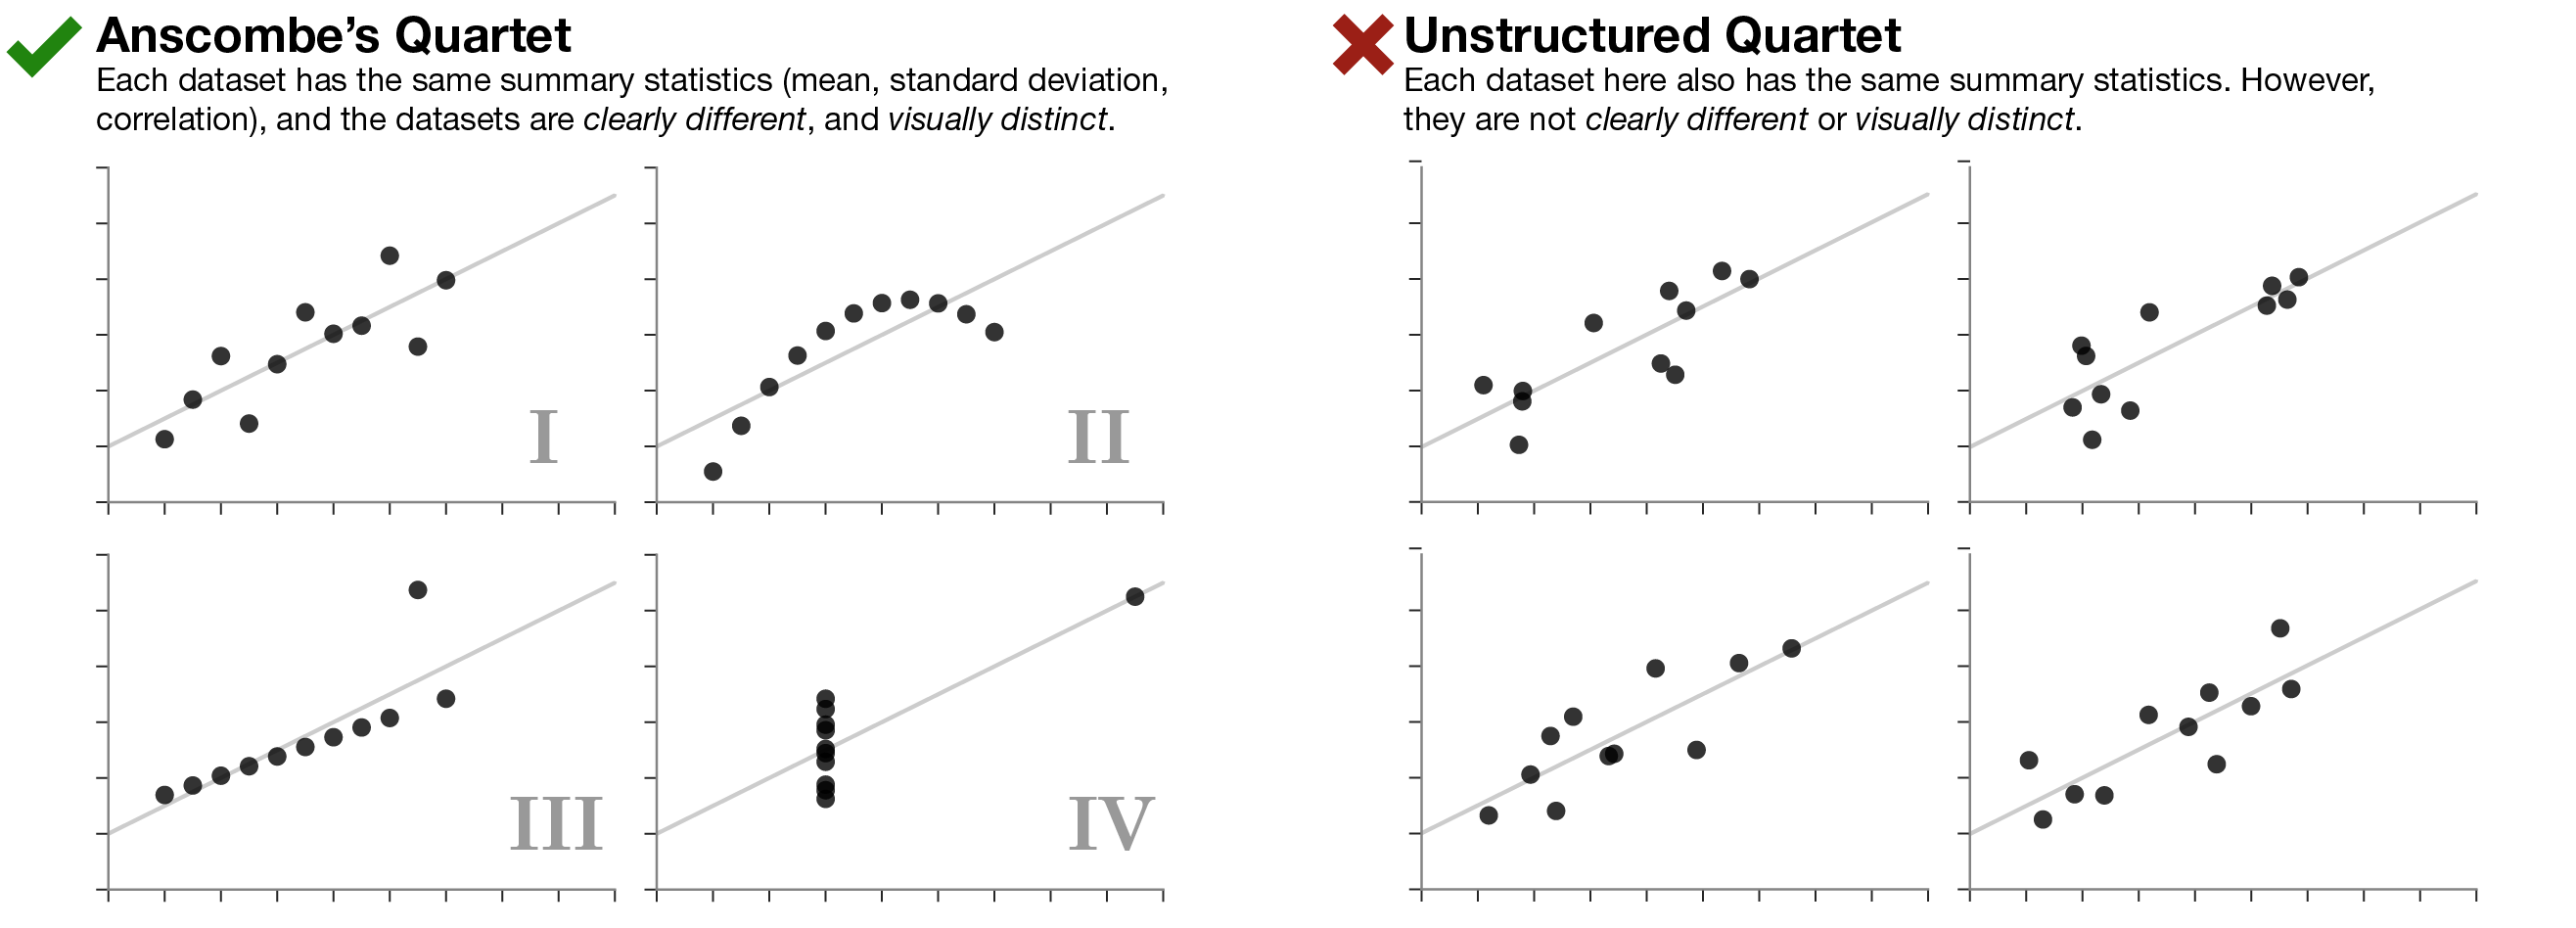
\includegraphics[width=36.56in]{figures/anscombe} \caption{Anscombe's quartet.}\label{fig:visualization1-02}
\end{figure}

Anscombe's quartet in Figure \ref{fig:visualization1-01} (left side) illustrates the importance of visualizing data. Even though the datasets I-IV have the same summary statistics (mean, standard deviation, correlation), they are importantly different from each other. On the right side, we have four data sets with the same summary statistics that are very similar to each other.

\begin{figure}
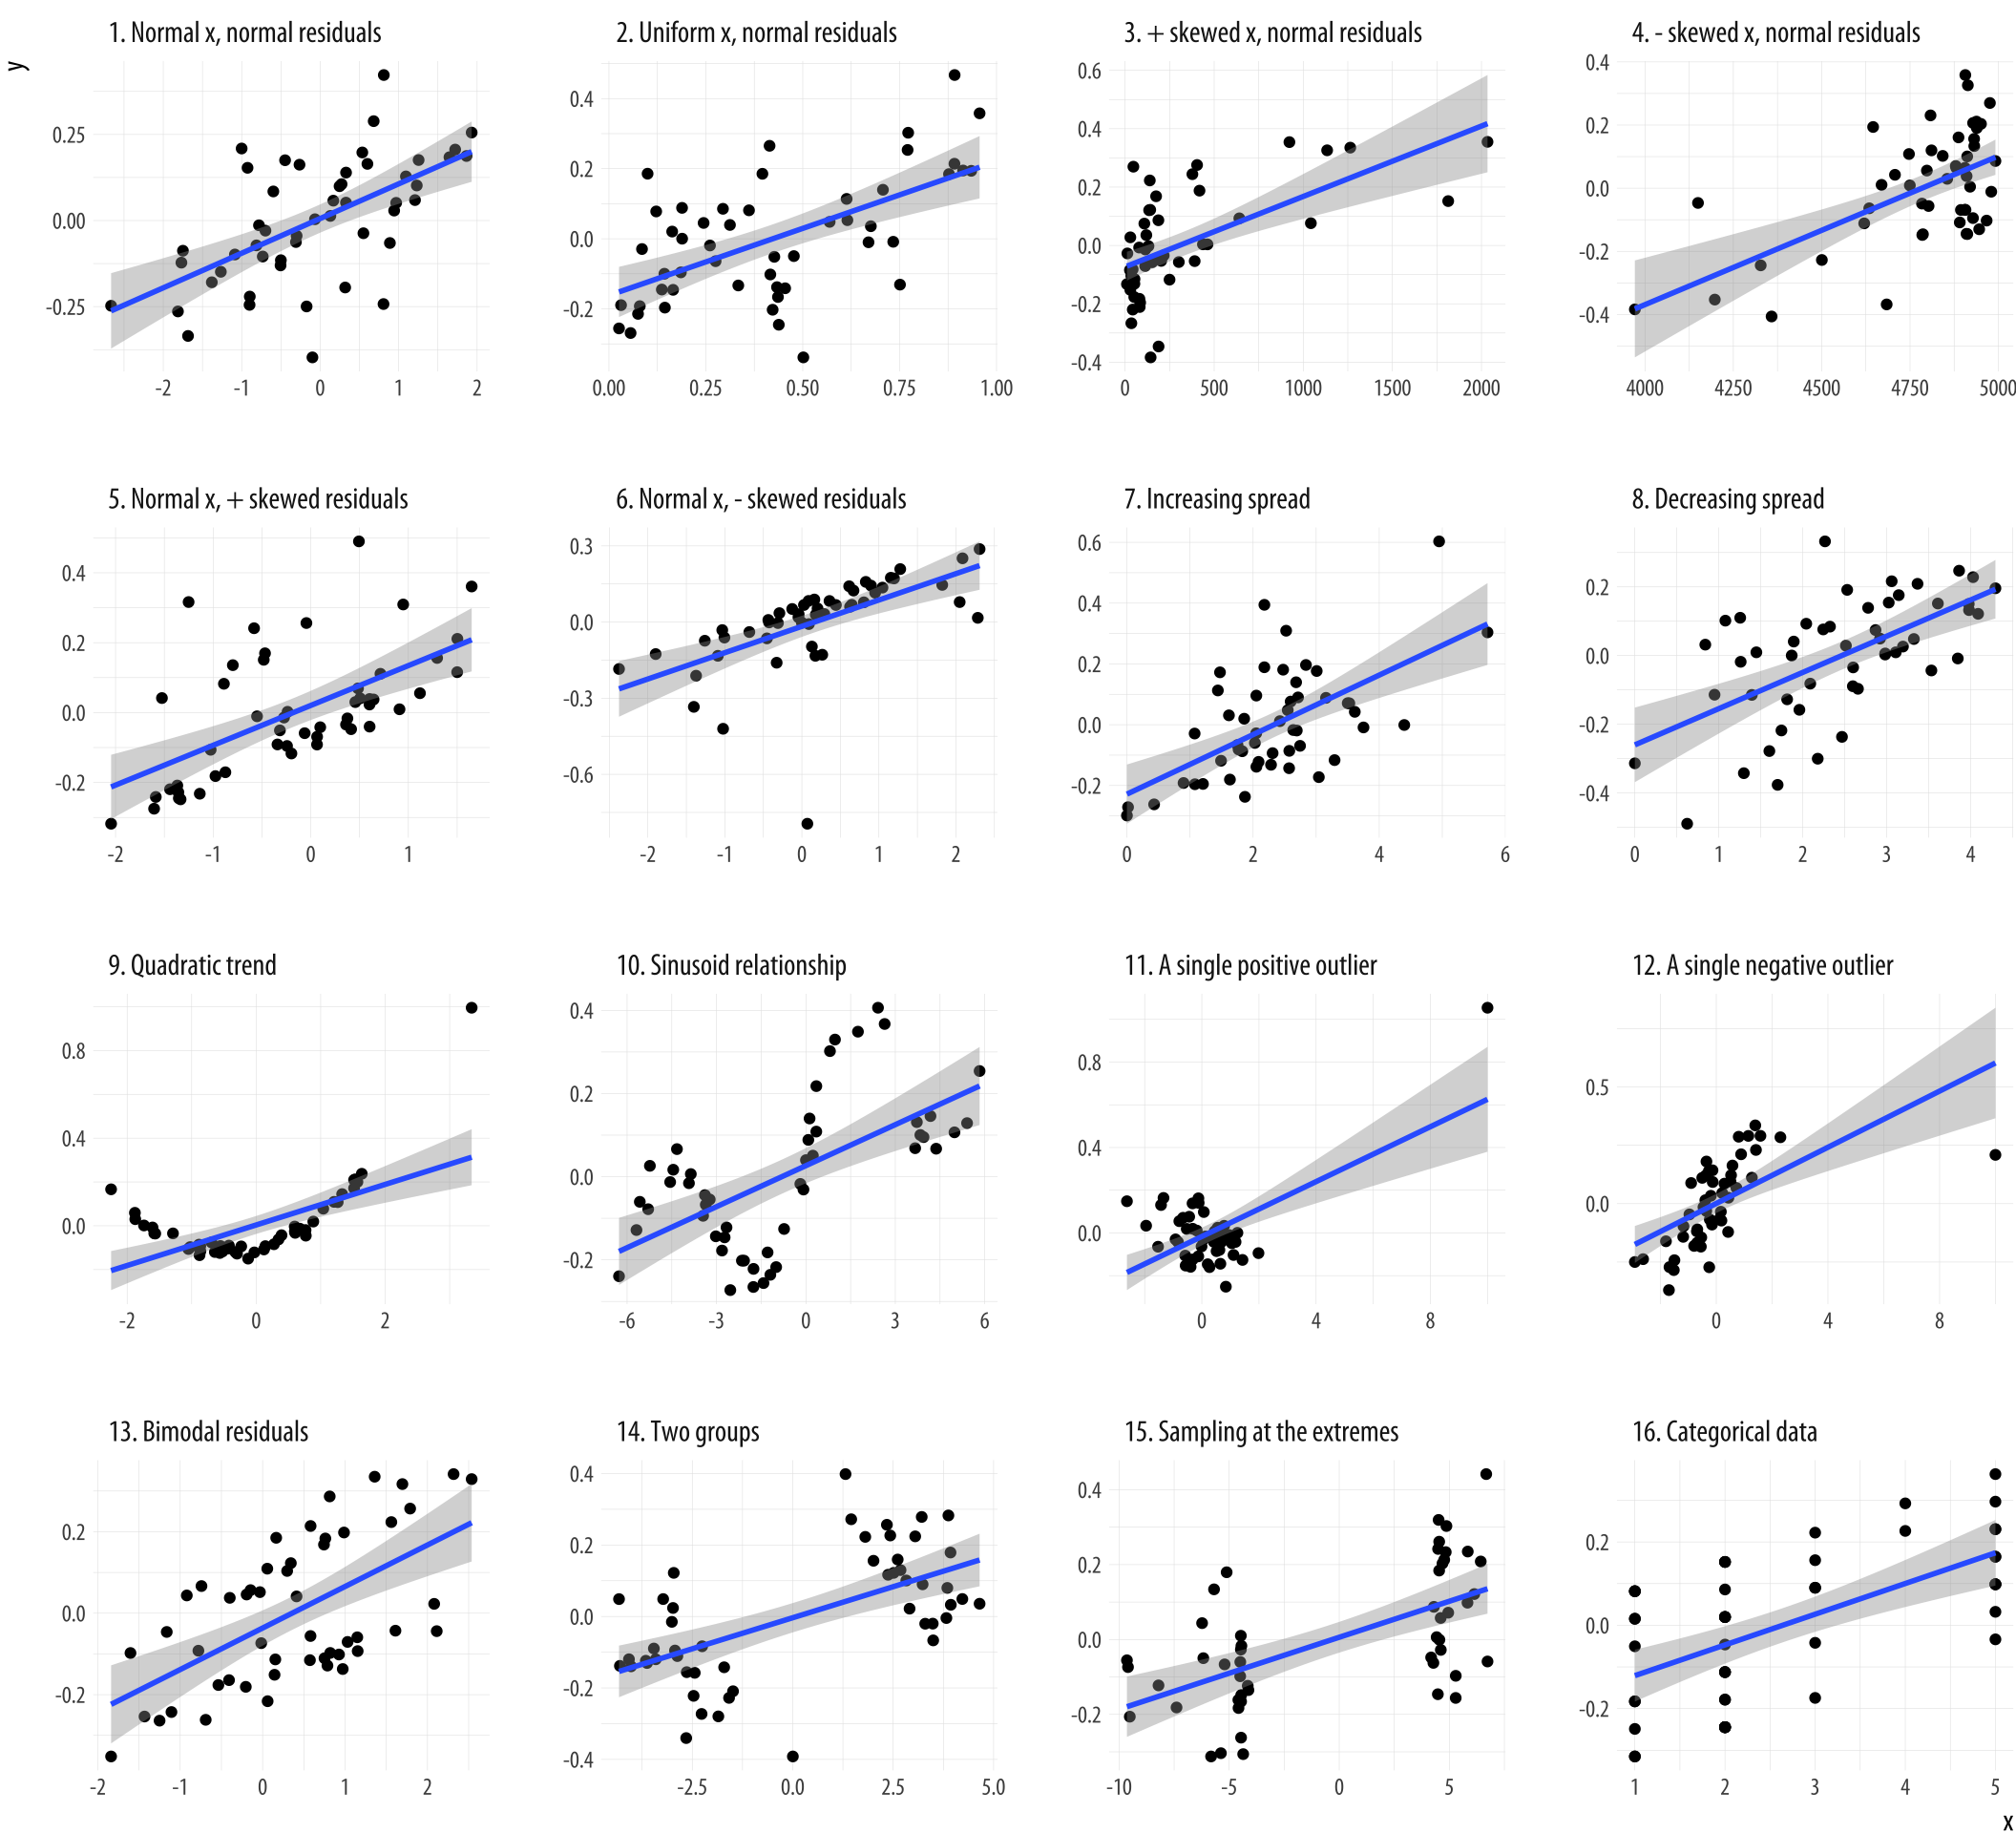
\includegraphics[width=29.33in]{figures/correlations} \caption{The Pearson's $r$ correlation coefficient is the same for all of these datasets. Source: [Data Visualization -- A practical introduction by Kieran Healy](http://socviz.co/lookatdata.html#lookatdata)}\label{fig:visualization1-03}
\end{figure}

All the datasets in Figure \ref{fig:visualization1-03} share the same correlation coefficient. However, again, they are very different from each other.

\textbackslash begin\{figure\}
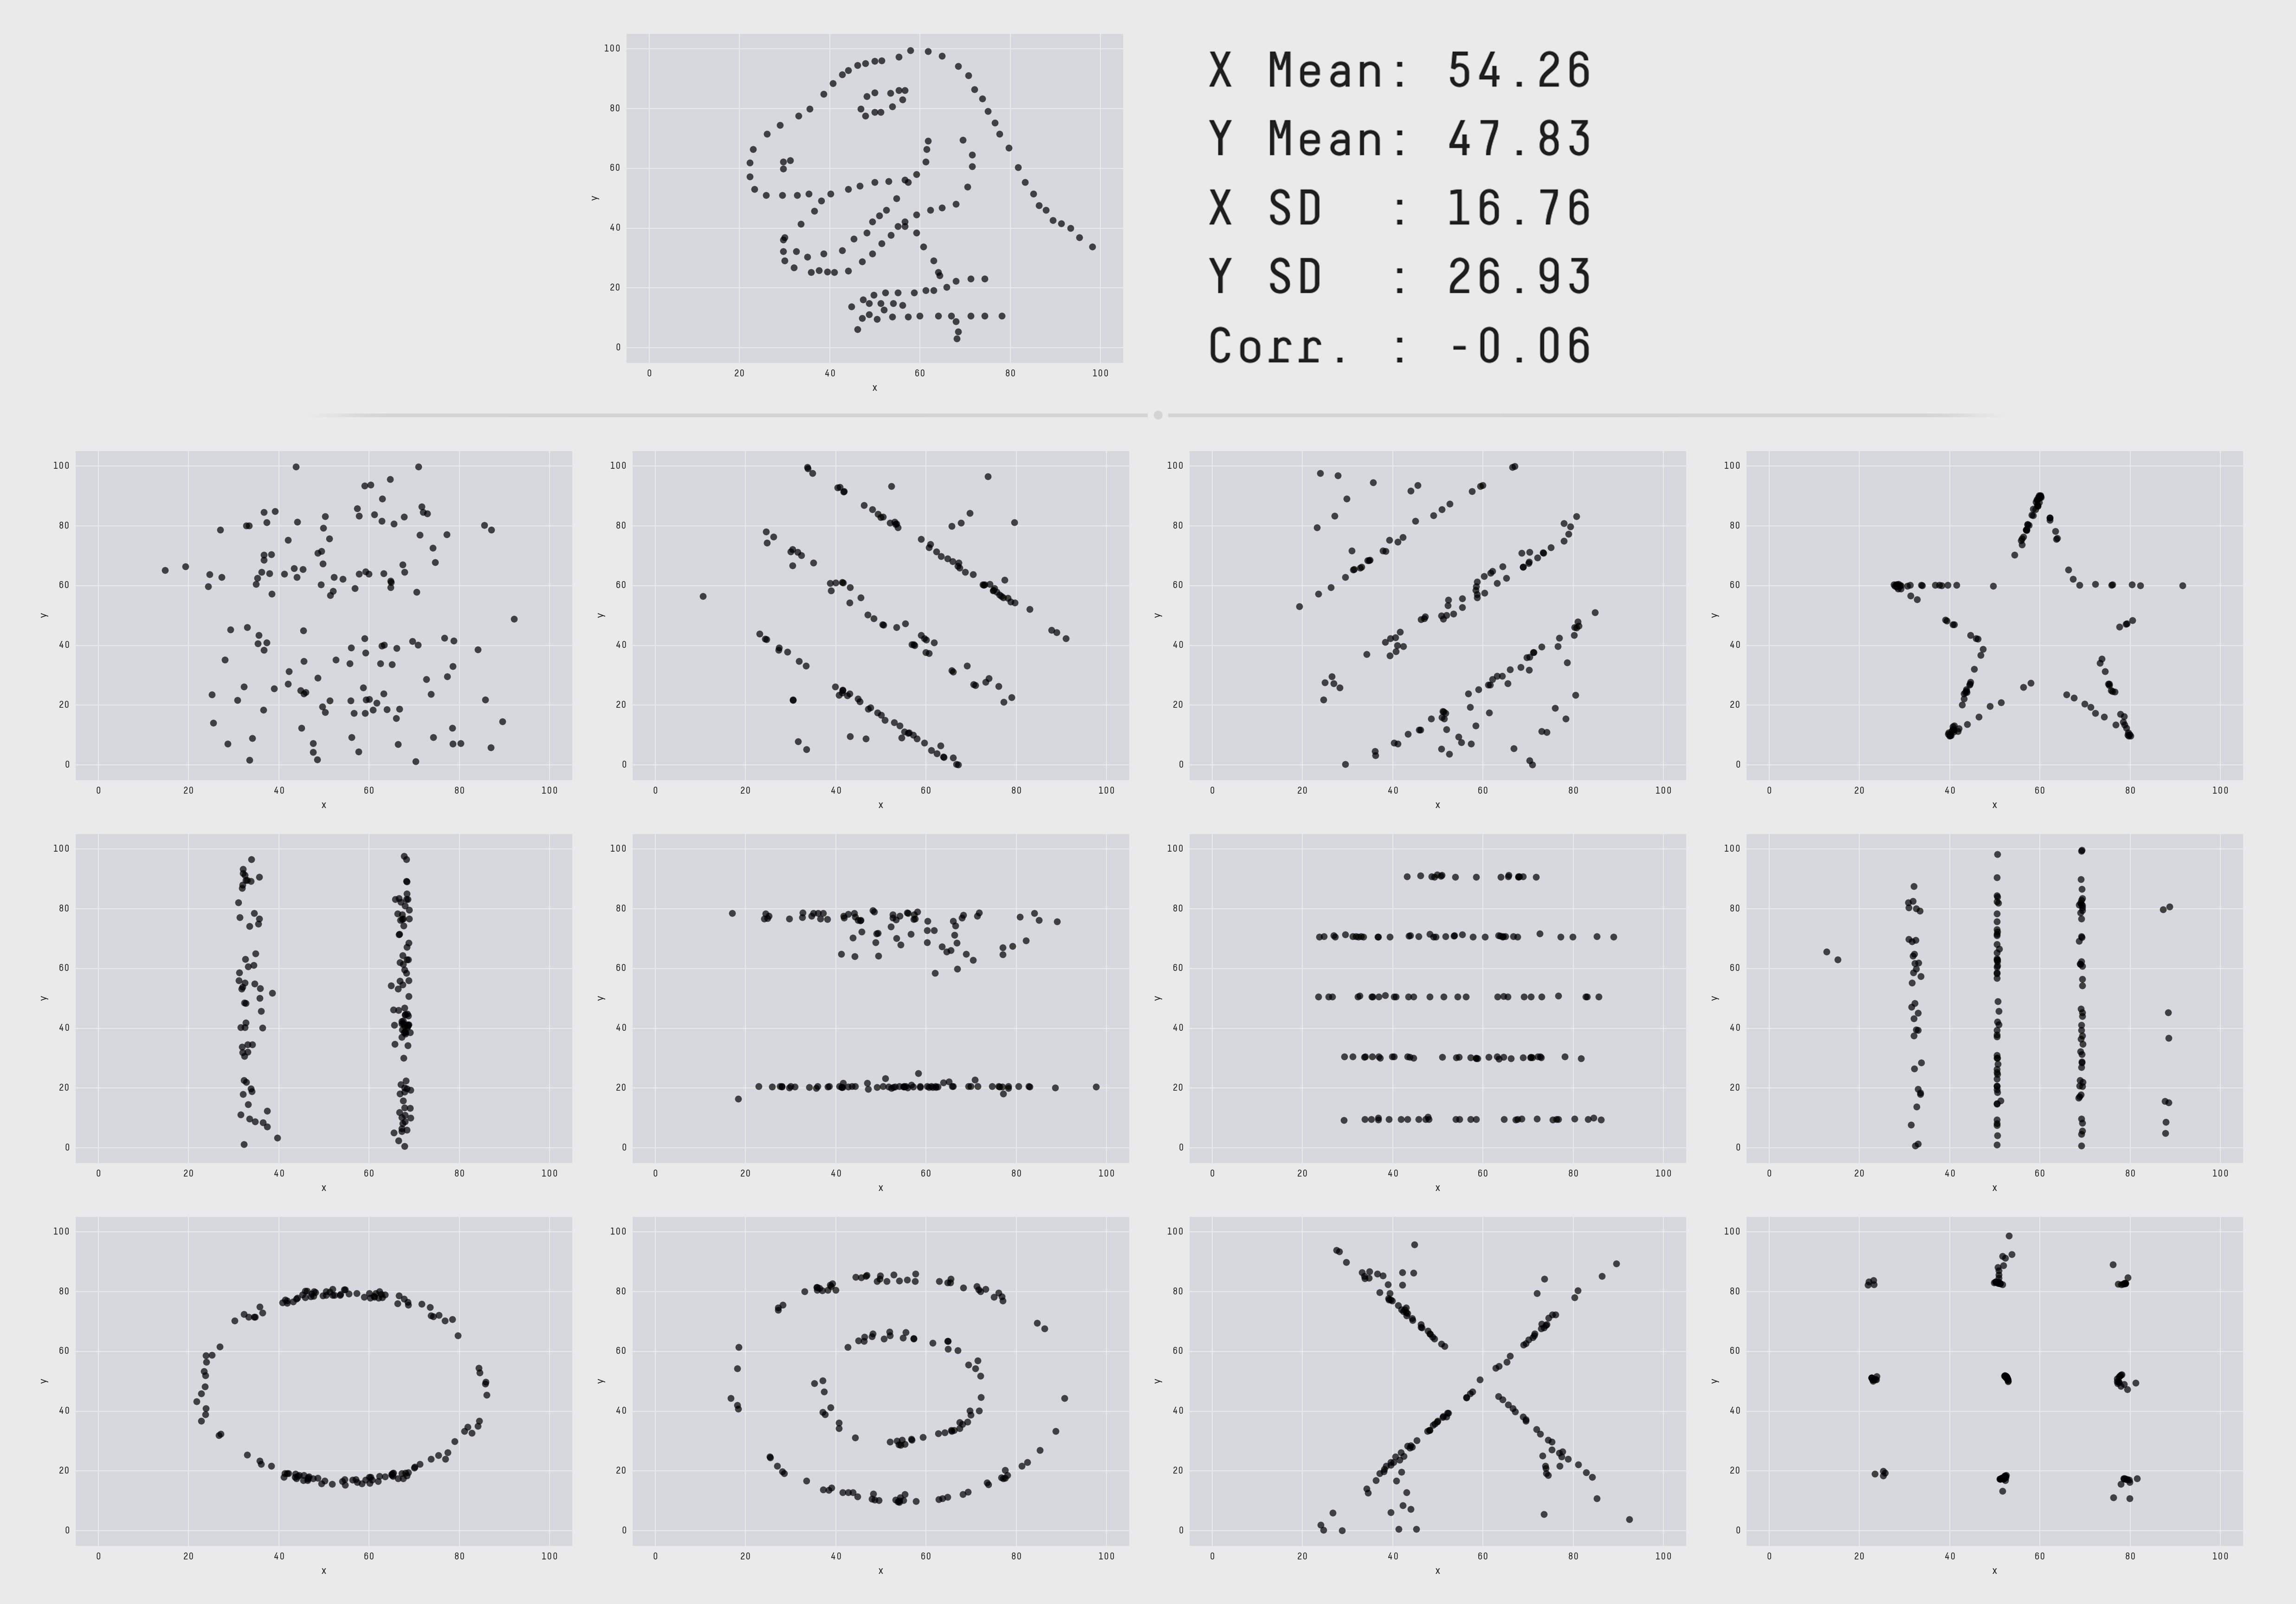
\includegraphics[width=68.71in]{figures/datasaurus_dozen} \textbackslash caption\{\textbf{The Datasaurus Dozen}. While different in appearance, each dataset has the same summary statistics to two decimal places (mean, standard deviation, and Pearson's correlation).\}\label{fig:visualization1-04}
\textbackslash end\{figure\}

The data sets in Figure \ref{fig:visualization1-04} all share the same summary statistics. Clearly, the data sets are not the same though.

\begin{quote}
\textbf{Tip}: Always plot the data first!
\end{quote}

\href{https://www.autodeskresearch.com/publications/samestats}{Here} is the paper from which I took Figure \ref{fig:visualization1-02} and \ref{fig:visualization1-04}. It explains how the figures were generated and shows more examples for how summary statistics and some kinds of plots are insufficient to get a good sense for what's going on in the data.

\begin{figure}
\centering
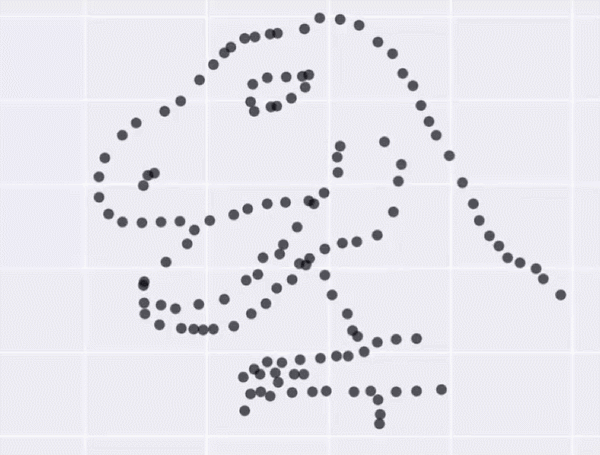
\includegraphics{figures/data_dino.gif}
\caption{\label{fig:visualization1-05}Animation showing different data sets that all share the same summary statistics.}
\end{figure}

\hypertarget{how-not-to-visualize-data}{%
\subsection{\texorpdfstring{How \emph{not} to visualize data}{How not to visualize data}}\label{how-not-to-visualize-data}}

Below are some examples of visualizations that could be improved. How would you make them better?

\begin{figure}

{\centering 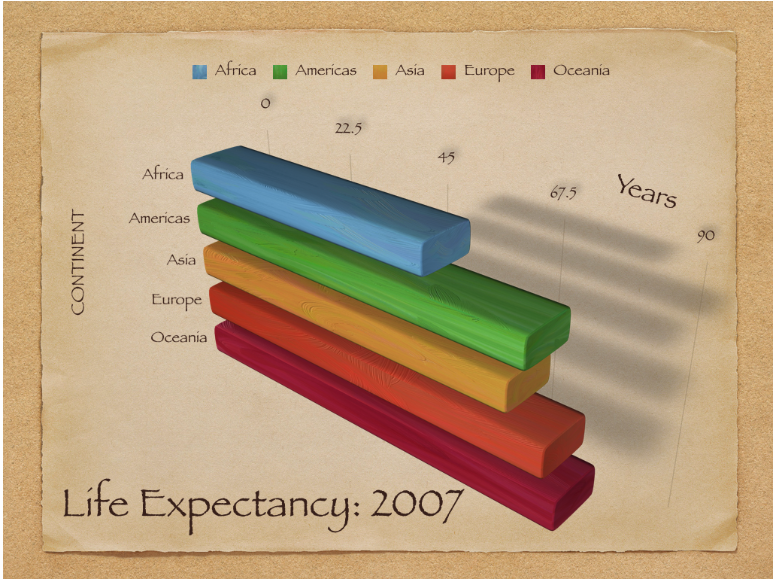
\includegraphics[width=0.9\linewidth]{figures/bad_plot1} 

}

\caption{Example of a bad plot. Source: [Data Visualization -- A practical introduction by Kieran Healy](http://socviz.co/lookatdata.html#lookatdata)}\label{fig:visualization1-06}
\end{figure}

\begin{figure}

{\centering 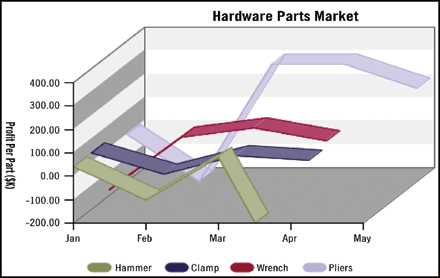
\includegraphics[width=0.9\linewidth]{figures/bad_plot2} 

}

\caption{Another bad plot. Source: Google image search for 'bad graphs'}\label{fig:visualization1-07}
\end{figure}

\textbackslash begin\{figure\}

\{\centering 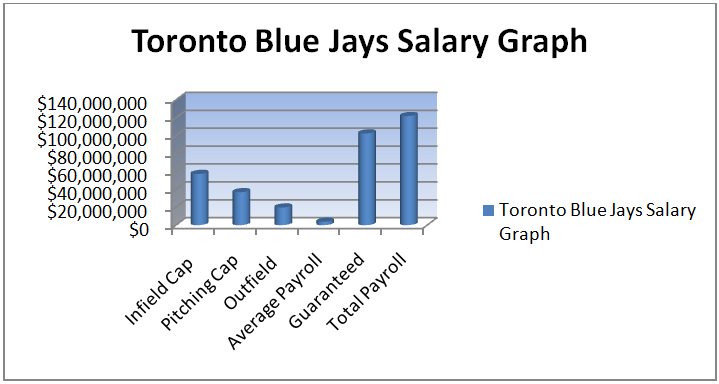
\includegraphics[width=0.9\linewidth]{figures/bad_plot3}

\}

\textbackslash caption\{And another one. Source: \href{http://bcuchta.com/wall_of_shame/}{Bad graph wall of shame}\}\label{fig:visualization1-08}
\textbackslash end\{figure\}

\textbackslash begin\{figure\}

\{\centering 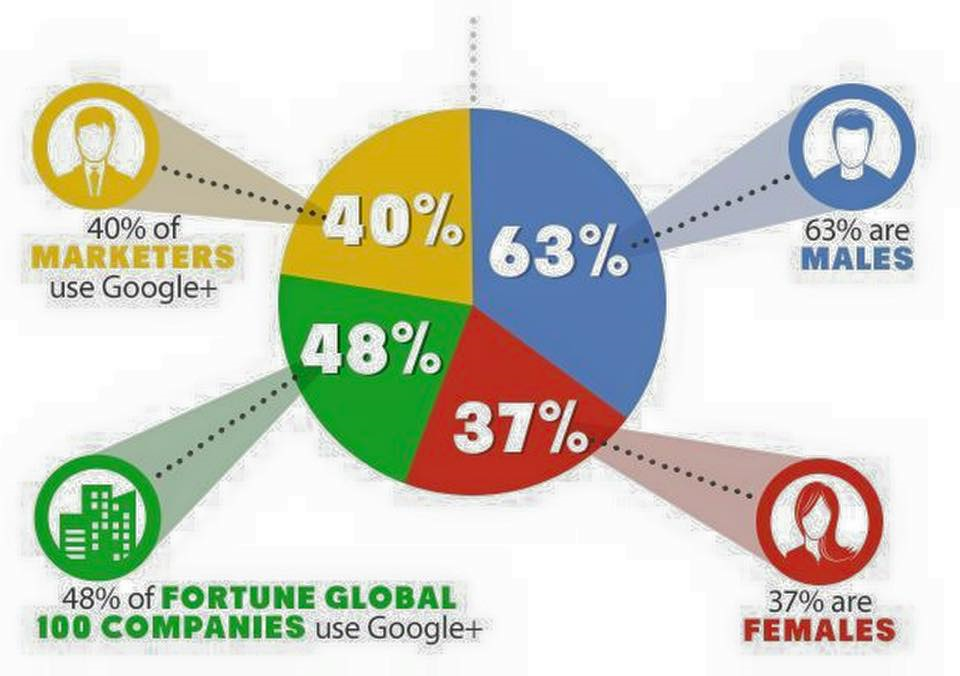
\includegraphics[width=0.9\linewidth]{figures/bad_plot4}

\}

\textbackslash caption\{And another one. Source: \href{http://bcuchta.com/wall_of_shame/}{Bad graph wall of shame}\}\label{fig:visualization1-09}
\textbackslash end\{figure\}

\textbackslash begin\{figure\}

\{\centering 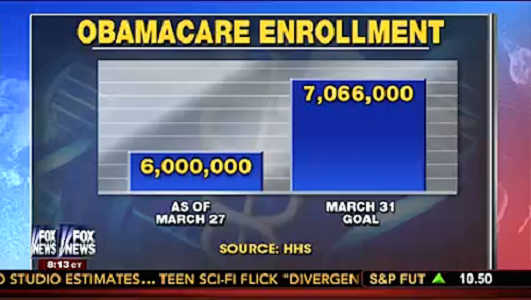
\includegraphics[width=0.9\linewidth]{figures/bad_plot5}

\}

\textbackslash caption\{And another one. Source: \href{http://bcuchta.com/wall_of_shame/}{Bad graph wall of shame}\}\label{fig:visualization1-10}
\textbackslash end\{figure\}

\textbackslash begin\{figure\}

\{\centering 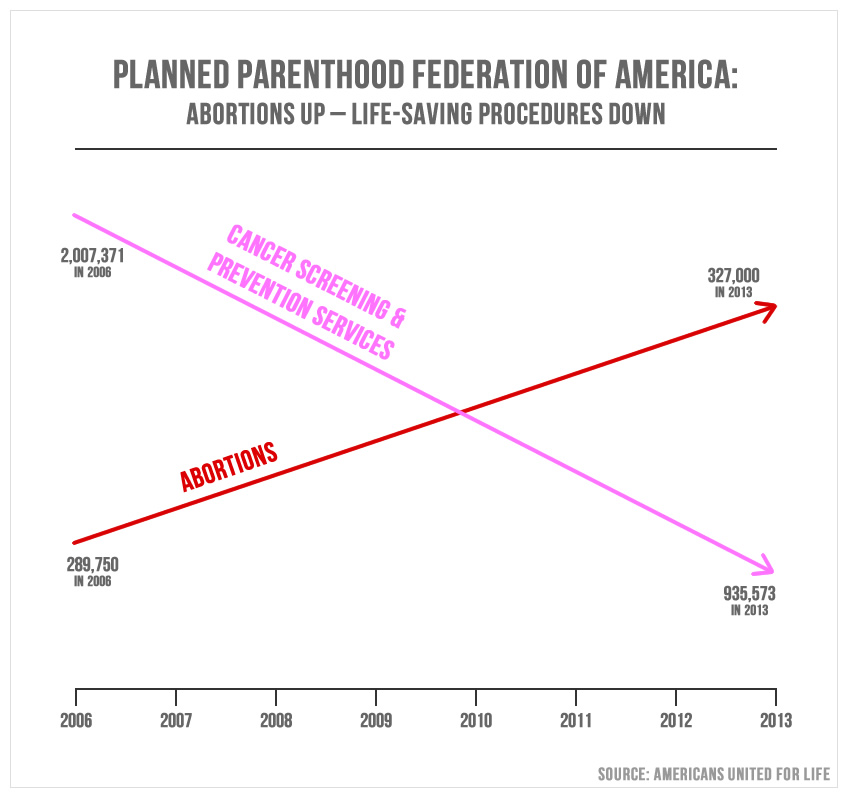
\includegraphics[width=0.9\linewidth]{figures/bad_plot6}

\}

\textbackslash caption\{The last one for now. Source: \href{http://bcuchta.com/wall_of_shame/}{Bad graph wall of shame}\}\label{fig:visualization1-11}
\textbackslash end\{figure\}

\hypertarget{how-to-make-it-better}{%
\subsection{How to make it better}\label{how-to-make-it-better}}

In this class, we you will learn how to use \texttt{ggplot2} to make nice figures. The \texttt{ggplot2} library provides a unified framework for making plots -- it defines a grammar of graphics according to which we construct figures step by step.

Instead of learning rigid rules for what makes for a good figure, you will learn how to make figures yourself, play around with things, and get a feeling for what works best.

\hypertarget{setting-up-rstudio}{%
\section{Setting up RStudio}\label{setting-up-rstudio}}

\begin{figure}
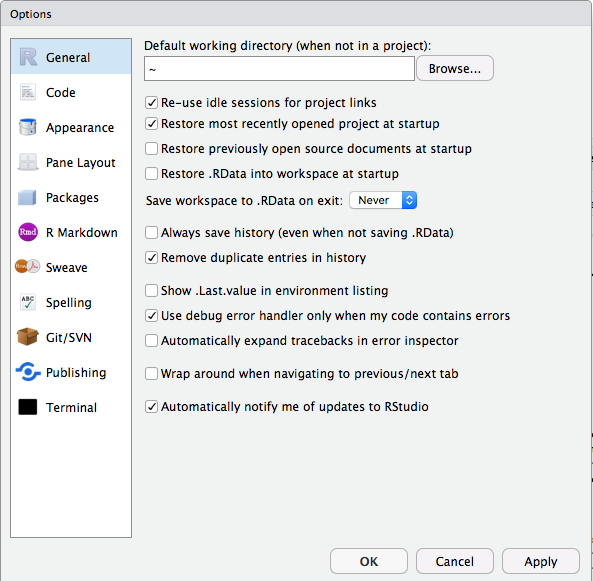
\includegraphics[width=1\linewidth]{figures/r_preferences_general} \caption{General preferences.}\label{fig:visualization1-12}
\end{figure}

\textbf{Make sure that}:

\begin{itemize}
\tightlist
\item
  Restore .RData into workspace at startup is \emph{unselected}
\item
  Save workspace to .RData on exit is set to \emph{Never}
\end{itemize}

\begin{figure}
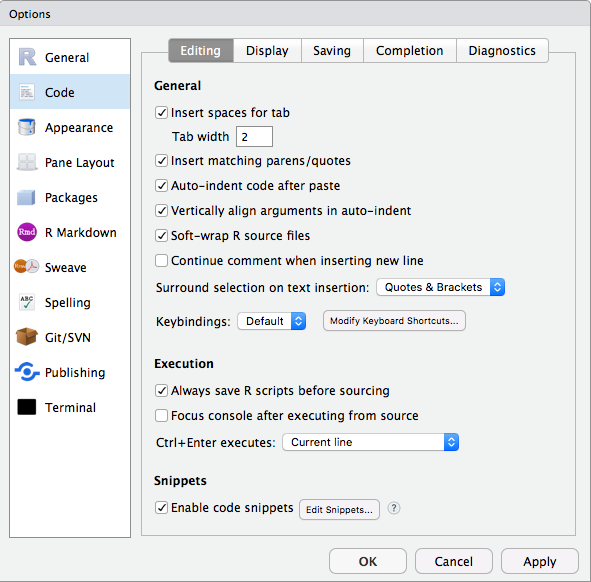
\includegraphics[width=1\linewidth]{figures/r_preferences_code} \caption{Code window preferences.}\label{fig:visualization1-13}
\end{figure}

\textbf{Make sure that}:

\begin{itemize}
\tightlist
\item
  Soft-wrap R source files is \emph{selected}
\end{itemize}

This way you don't have to scroll horizontally. At the same time, avoid writing long single lines of code. For example, instead of writing code like so:

\begin{Shaded}
\begin{Highlighting}[]
\KeywordTok{ggplot}\NormalTok{(}\DataTypeTok{data =}\NormalTok{ diamonds, }\KeywordTok{aes}\NormalTok{(}\DataTypeTok{x =}\NormalTok{ cut, }\DataTypeTok{y =}\NormalTok{ price)) }\OperatorTok{+}
\StringTok{  }\KeywordTok{stat_summary}\NormalTok{(}\DataTypeTok{fun.y =} \StringTok{"mean"}\NormalTok{, }\DataTypeTok{geom =} \StringTok{"bar"}\NormalTok{, }\DataTypeTok{color =} \StringTok{"black"}\NormalTok{, }\DataTypeTok{fill =} \StringTok{"lightblue"}\NormalTok{, }\DataTypeTok{width =} \FloatTok{0.85}\NormalTok{) }\OperatorTok{+}
\StringTok{  }\KeywordTok{stat_summary}\NormalTok{(}\DataTypeTok{fun.data =} \StringTok{"mean_cl_boot"}\NormalTok{, }\DataTypeTok{geom =} \StringTok{"linerange"}\NormalTok{, }\DataTypeTok{size =} \FloatTok{1.5}\NormalTok{) }\OperatorTok{+}
\StringTok{  }\KeywordTok{labs}\NormalTok{(}\DataTypeTok{title =} \StringTok{"Price as a function of quality of cut"}\NormalTok{, }\DataTypeTok{subtitle =} \StringTok{"Note: The price is in US dollars"}\NormalTok{, }\DataTypeTok{tag =} \StringTok{"A"}\NormalTok{, }\DataTypeTok{x =} \StringTok{"Quality of the cut"}\NormalTok{, }\DataTypeTok{y =} \StringTok{"Price"}\NormalTok{)}
\end{Highlighting}
\end{Shaded}

You may want to write it this way instead:

\begin{Shaded}
\begin{Highlighting}[]
\KeywordTok{ggplot}\NormalTok{(}\DataTypeTok{data =}\NormalTok{ diamonds, }\KeywordTok{aes}\NormalTok{(}\DataTypeTok{x =}\NormalTok{ cut, }\DataTypeTok{y =}\NormalTok{ price)) }\OperatorTok{+}
\StringTok{  }\CommentTok{# display the means}
\StringTok{  }\KeywordTok{stat_summary}\NormalTok{(}\DataTypeTok{fun.y =} \StringTok{"mean"}\NormalTok{,}
               \DataTypeTok{geom =} \StringTok{"bar"}\NormalTok{,}
               \DataTypeTok{color =} \StringTok{"black"}\NormalTok{,}
               \DataTypeTok{fill =} \StringTok{"lightblue"}\NormalTok{,}
               \DataTypeTok{width =} \FloatTok{0.85}\NormalTok{) }\OperatorTok{+}
\StringTok{  }\CommentTok{# display the error bars}
\StringTok{  }\KeywordTok{stat_summary}\NormalTok{(}\DataTypeTok{fun.data =} \StringTok{"mean_cl_boot"}\NormalTok{,}
               \DataTypeTok{geom =} \StringTok{"linerange"}\NormalTok{,}
               \DataTypeTok{size =} \FloatTok{1.5}\NormalTok{) }\OperatorTok{+}
\StringTok{  }\CommentTok{# change labels}
\StringTok{  }\KeywordTok{labs}\NormalTok{(}\DataTypeTok{title =} \StringTok{"Price as a function of quality of cut"}\NormalTok{,}
       \DataTypeTok{subtitle =} \StringTok{"Note: The price is in US dollars"}\NormalTok{, }\CommentTok{# we might want to change this later}
       \DataTypeTok{tag =} \StringTok{"A"}\NormalTok{,}
       \DataTypeTok{x =} \StringTok{"Quality of the cut"}\NormalTok{,}
       \DataTypeTok{y =} \StringTok{"Price"}\NormalTok{)}
\end{Highlighting}
\end{Shaded}

This makes it much easier to see what's going on, and you can easily add comments to individual lines of code.

RStudio makes it easy to write nice code. It figures out where to put the next line of code when you press \texttt{ENTER}. And if things ever get messy, just select the code of interest and hit \texttt{cmd+i} to re-indent the code.

Here are some more resources with tips for how to write nice code in R:

\begin{itemize}
\tightlist
\item
  \href{http://adv-r.had.co.nz/Style.html}{Advanced R style guide}
\end{itemize}

\hypertarget{getting-help}{%
\section{Getting help}\label{getting-help}}

There are three simple ways to get help in R. You can either put a \texttt{?} in front of the function you'd like to learn more about, or use the \texttt{help()} function.

\begin{Shaded}
\begin{Highlighting}[]
\NormalTok{?print}
\KeywordTok{help}\NormalTok{(}\StringTok{"print"}\NormalTok{)}
\end{Highlighting}
\end{Shaded}

\begin{quote}
\textbf{Tip}: To see the help file, hover over a function (or dataset) with the mouse (or select the text) and then press \texttt{F1}.
\end{quote}

I recommend using \texttt{F1} to get to help files -- it's the fastest way!

R help files can sometimes look a little cryptic. Most R help files have the following sections (copied from \href{https://www.dummies.com/programming/r/r-for-dummies-cheat-sheet/}{here}):

\begin{center}\rule{0.5\linewidth}{\linethickness}\end{center}

\textbf{Title}: A one-sentence overview of the function.

\textbf{Description}: An introduction to the high-level objectives of the function, typically about one paragraph long.

\textbf{Usage}: A description of the syntax of the function (in other words, how the function is called). This is where you find all the arguments that you can supply to the function, as well as any default values of these arguments.

\textbf{Arguments}: A description of each argument. Usually this includes a specification of the class (for example, character, numeric, list, and so on). This section is an important one to understand, because arguments are frequently a cause of errors in R.

\textbf{Details}: Extended details about how the function works, provides longer descriptions of the various ways to call the function (if applicable), and a longer discussion of the arguments.

\textbf{Value}: A description of the class of the value returned by the function.

\textbf{See also}: Links to other relevant functions. In most of the R editors, you can click these links to read the Help files for these functions.

\textbf{Examples}: Worked examples of real R code that you can paste into your console and run.

\begin{center}\rule{0.5\linewidth}{\linethickness}\end{center}

Here is the help file for the \texttt{print()} function:

\begin{figure}
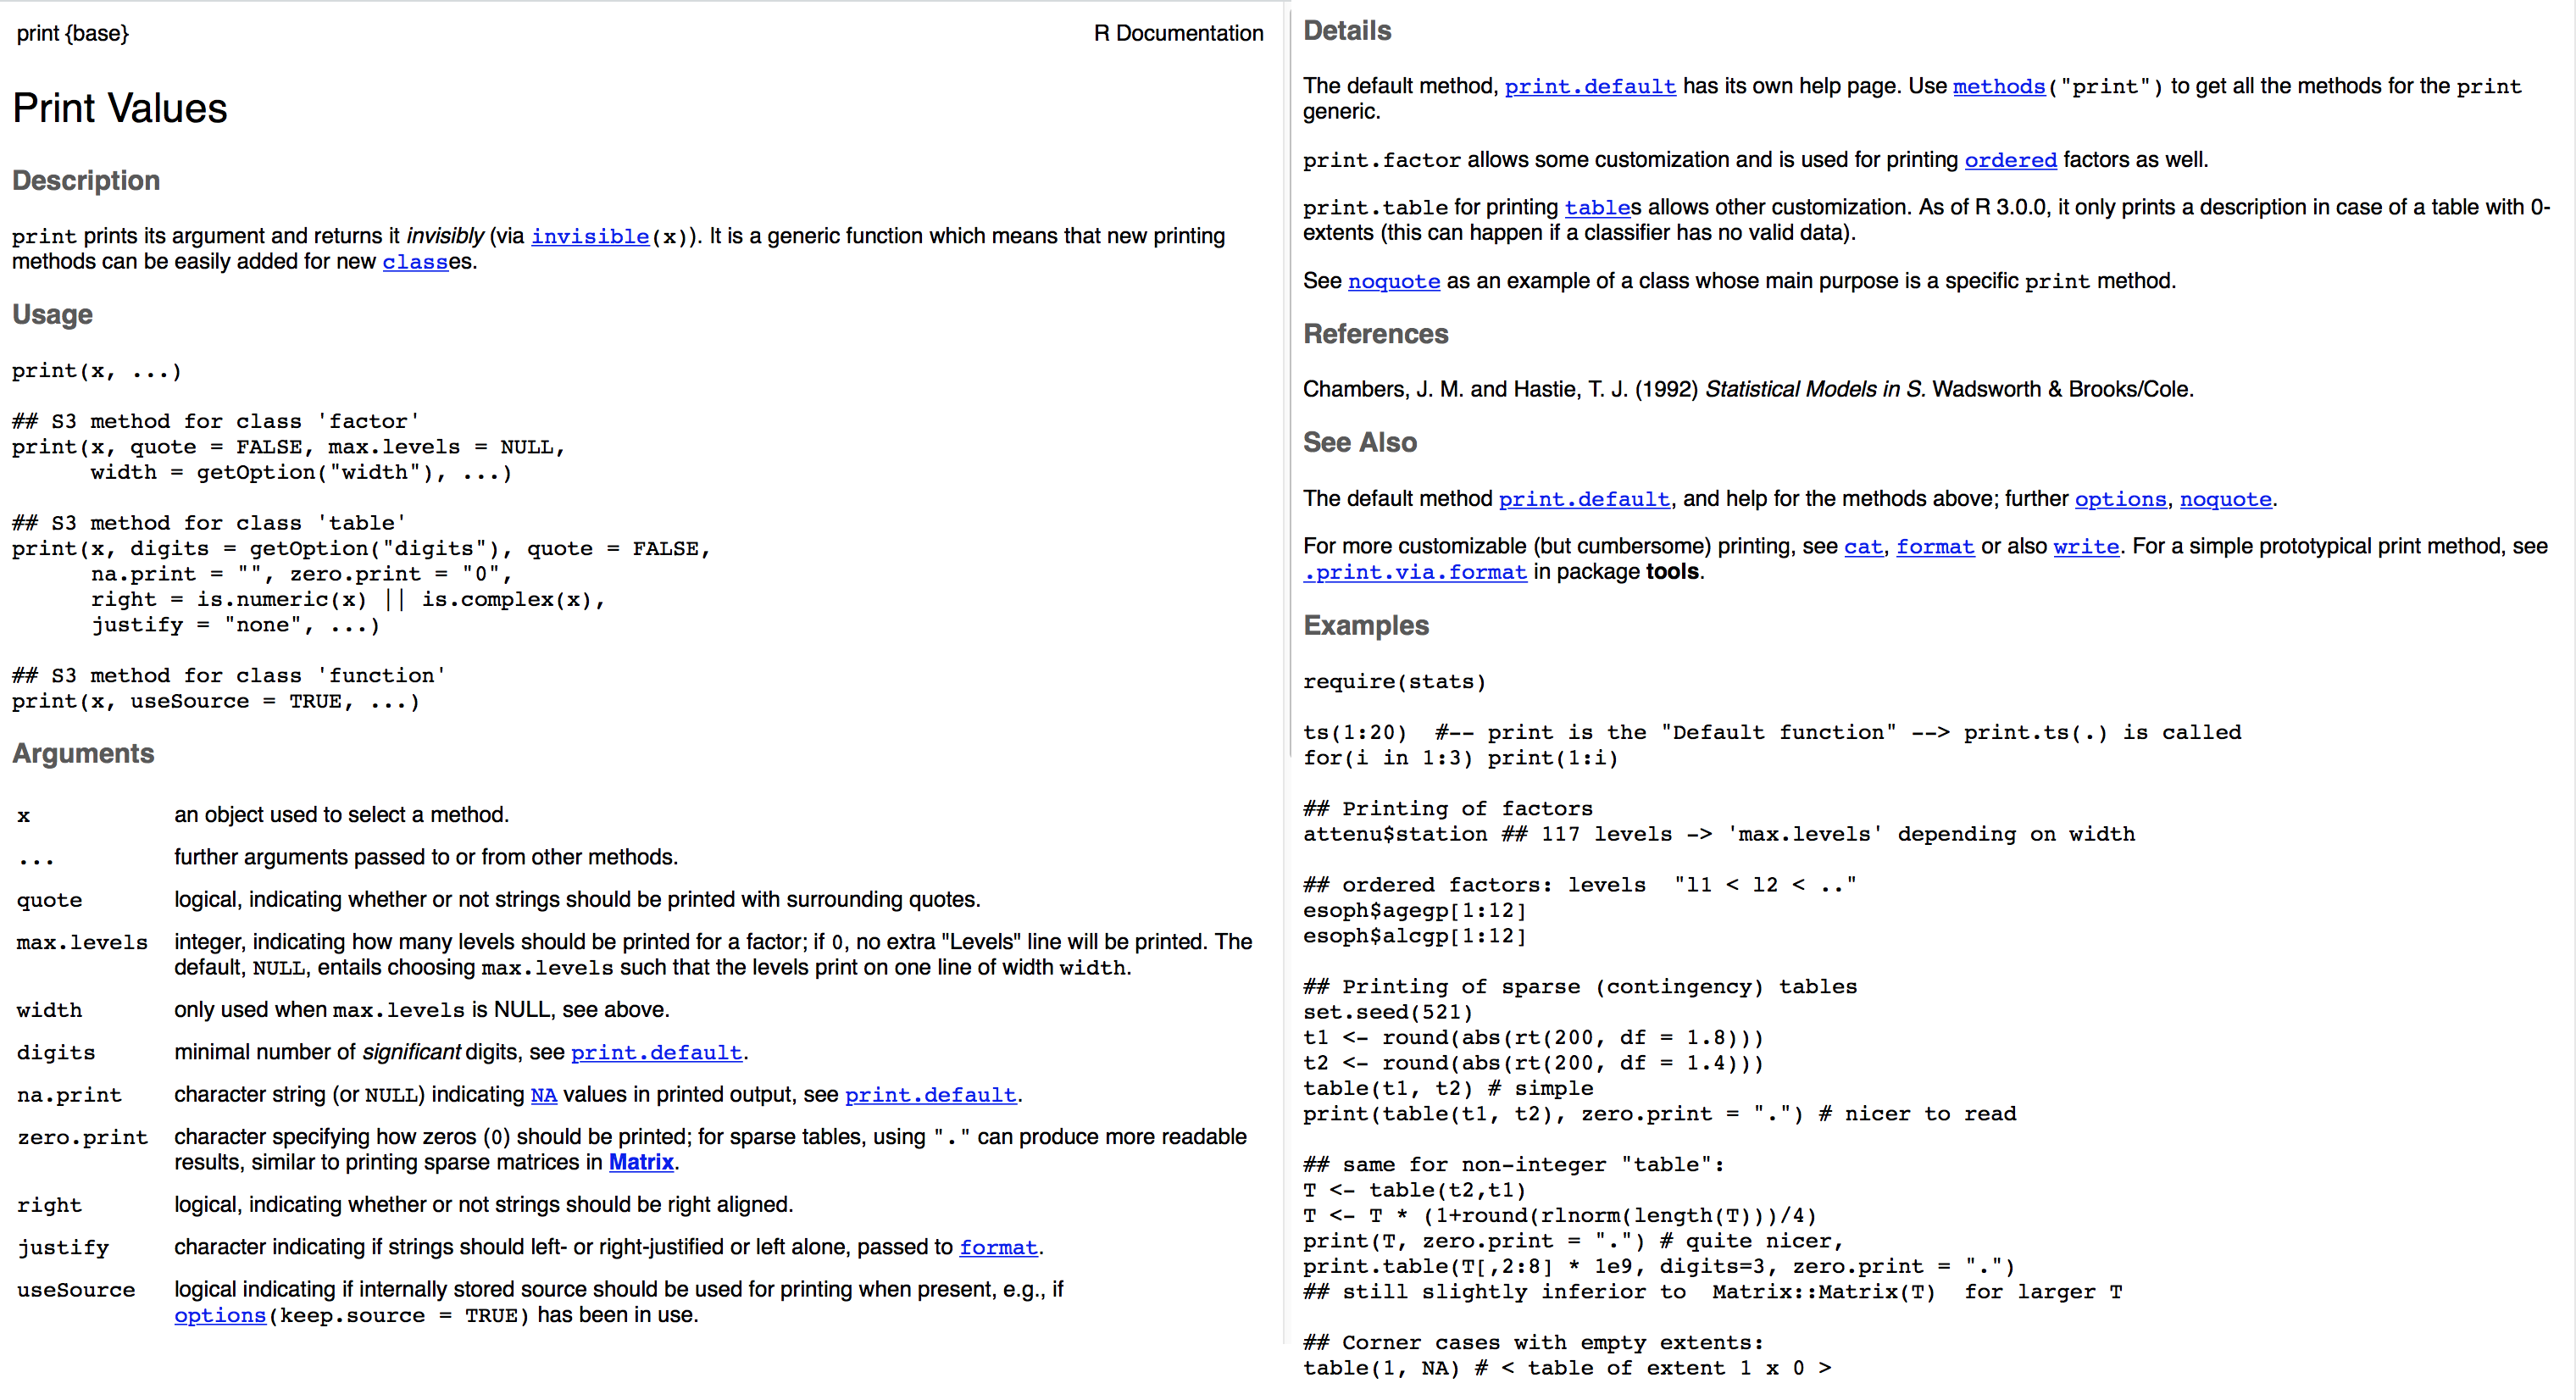
\includegraphics[width=42.22in]{figures/help_print} \caption{Help file for the print() function.}\label{fig:visualization1-17}
\end{figure}

\hypertarget{data-visualization-using-ggplot2}{%
\section{\texorpdfstring{Data visualization using \texttt{ggplot2}}{Data visualization using ggplot2}}\label{data-visualization-using-ggplot2}}

We will use the \texttt{ggplot2} package to visualize data. By the end of next class, you'll be able to make a figure like this:

\begin{figure}
\centering
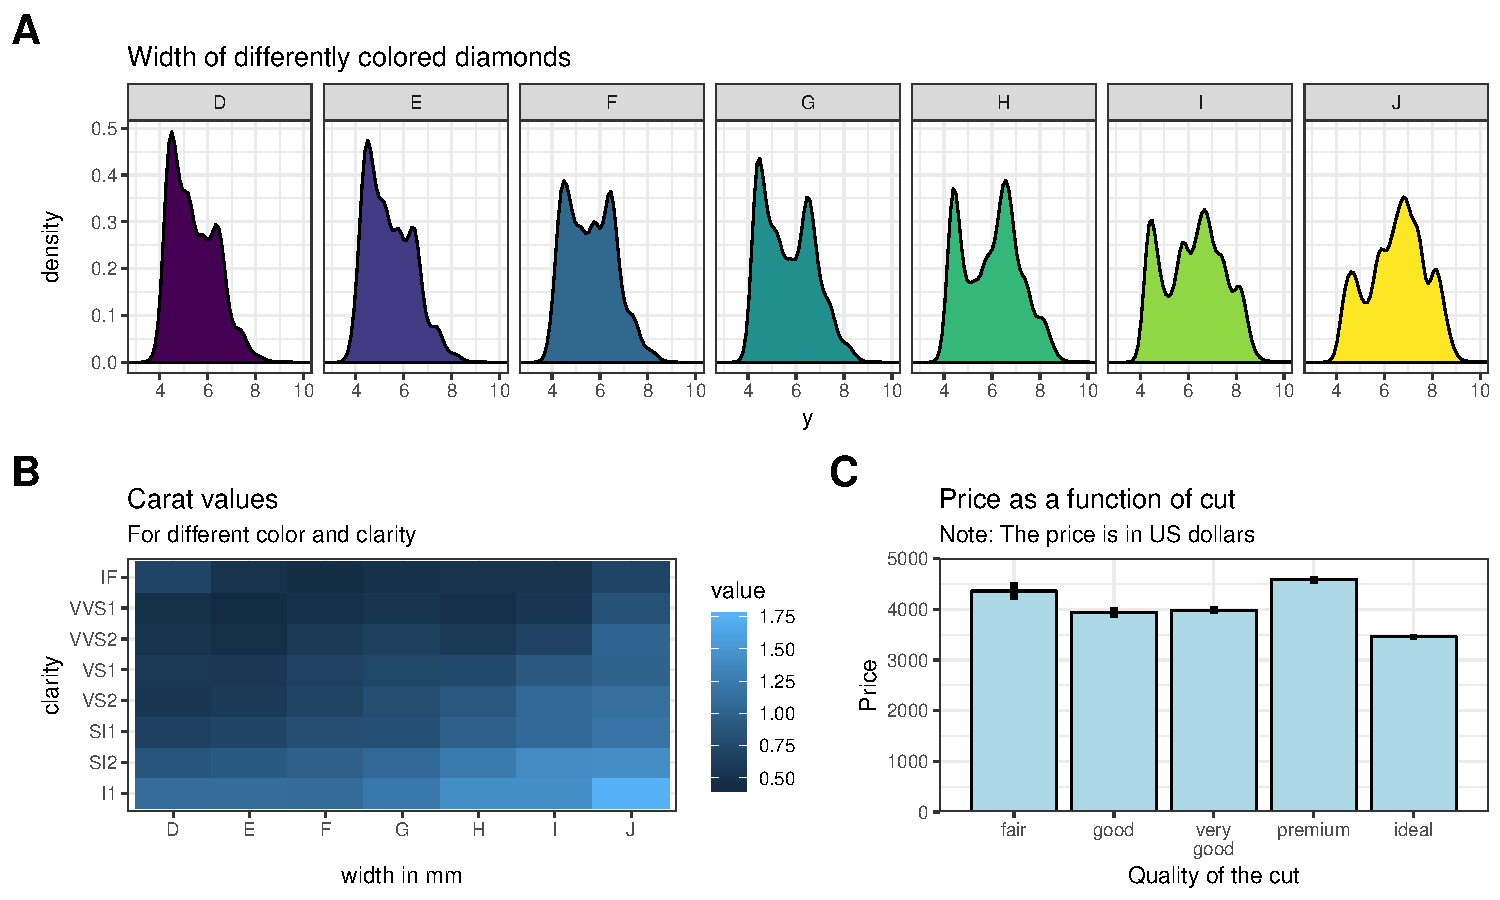
\includegraphics{figures/combined_plot.pdf}
\caption{\label{fig:visualization1-18}What a nice figure!}
\end{figure}

Now let's figure out how to get there.

\hypertarget{setting-up-a-plot}{%
\subsection{Setting up a plot}\label{setting-up-a-plot}}

Let's first get some data.

\begin{Shaded}
\begin{Highlighting}[]
\NormalTok{df.diamonds =}\StringTok{ }\NormalTok{diamonds}
\end{Highlighting}
\end{Shaded}

The \texttt{diamonds} dataset comes with the \texttt{ggplot2} package. We can get a description of the dataset by running the following command:

\begin{Shaded}
\begin{Highlighting}[]
\NormalTok{?diamonds}
\end{Highlighting}
\end{Shaded}

Above, we assigned the \texttt{diamonds} dataset to the variable \texttt{df.diamonds} so that we can see it in the data explorer.

Let's take a look at the full dataset by clicking on it in the explorer.

\begin{quote}
\textbf{Tip}: You can view a data frame by highlighting the text in the editor (or simply moving the mouse above the text), and then press \texttt{F2}.
\end{quote}

The \texttt{df.diamonds} data frame contains information about almost 60,000 diamonds, including their \texttt{price}, \texttt{carat} value, size, etc. Let's use visualization to get a better sense for this dataset.
We start by setting up the plot. To do so, we pass a data frame to the function \texttt{ggplot()} in the following way.

\begin{Shaded}
\begin{Highlighting}[]
\KeywordTok{ggplot}\NormalTok{(}\DataTypeTok{data =}\NormalTok{ df.diamonds)}
\end{Highlighting}
\end{Shaded}


\includegraphics{02-visualization1_files/figure-latex/visualization1-21-1.pdf}

This, by itself, won't do anything yet. We also need to specify what to plot.

Let's take a look at how much diamonds of different color cost. The help file says that diamonds labeled D have the best color, and diamonds labeled J the worst color. Let's make a bar plot that shows the average price of diamonds for different colors.

We do so via specifying a mapping from the data to the plot aesthetics with the function \texttt{aes()}. We need to tell \texttt{aes()} what we would like to display on the x-axis, and the y-axis of the plot.

\begin{Shaded}
\begin{Highlighting}[]
\KeywordTok{ggplot}\NormalTok{(}\DataTypeTok{data =}\NormalTok{ df.diamonds,}
       \DataTypeTok{mapping =} \KeywordTok{aes}\NormalTok{(}\DataTypeTok{x =}\NormalTok{ color, }\DataTypeTok{y =}\NormalTok{ price))}
\end{Highlighting}
\end{Shaded}

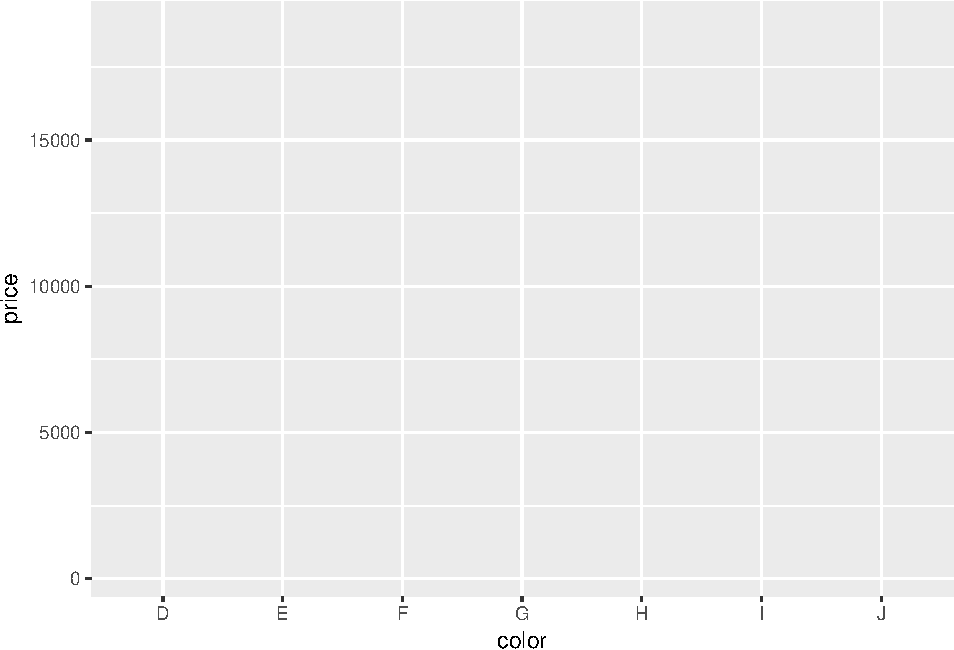
\includegraphics{02-visualization1_files/figure-latex/visualization1-22-1.pdf}

Here, we specified that we want to plot \texttt{color} on the x-axis, and \texttt{price} on the y-axis. As you can see, \texttt{ggplot2} has already figured out how to label the axes. However, we still need to specify \emph{how} to plot it. Let's make a \textbf{bar graph}:

\begin{Shaded}
\begin{Highlighting}[]
\KeywordTok{ggplot}\NormalTok{(}\DataTypeTok{data =}\NormalTok{ df.diamonds,}
       \DataTypeTok{mapping =} \KeywordTok{aes}\NormalTok{(}\DataTypeTok{x =}\NormalTok{ color, }\DataTypeTok{y =}\NormalTok{ price)) }\OperatorTok{+}
\StringTok{  }\KeywordTok{stat_summary}\NormalTok{(}\DataTypeTok{fun.y =} \StringTok{"mean"}\NormalTok{, }\DataTypeTok{geom =} \StringTok{"bar"}\NormalTok{)}
\end{Highlighting}
\end{Shaded}

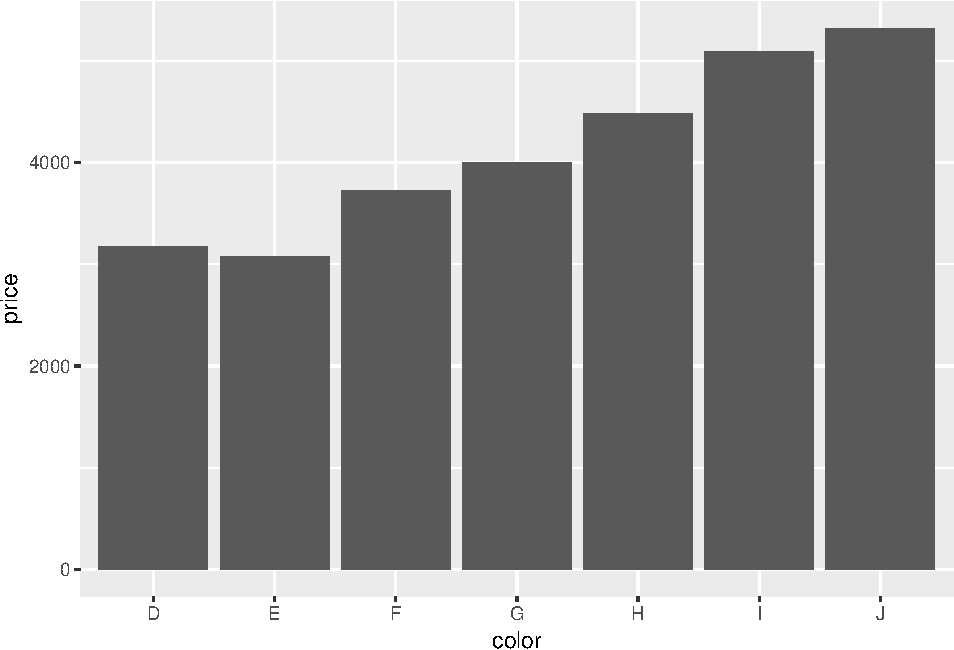
\includegraphics{02-visualization1_files/figure-latex/visualization1-23-1.pdf}

Neat! Three lines of code produce an almost-publication-ready plot (to be published in the \emph{Proceedings of Unnecessary Diamonds})! Note how we used a \texttt{+} at the end of the first line of code to specify that there will be more. This is a very powerful idea underlying \texttt{ggplot2}. We can start simple and keep adding things to the plot step by step.

We used the \texttt{stat\_summary()} function to define \emph{what} we want to plot (the ``mean''), and \emph{how} (as a ``bar'' chart). Let's take a closer look at that function.

\begin{Shaded}
\begin{Highlighting}[]
\KeywordTok{help}\NormalTok{(stat_summary)}
\end{Highlighting}
\end{Shaded}

Not the the easiest help file \ldots{} We supplied two arguments to the function, \texttt{fun.y\ =} and \texttt{geom\ =}.

\begin{enumerate}
\def\labelenumi{\arabic{enumi}.}
\tightlist
\item
  The \texttt{fun.y} argument specifies \emph{what} function we'd like to apply to the data for each value of \texttt{x}. Here, we said that we would like to take the \texttt{mean} and we specified that as a string.
\item
  The \texttt{geom} (= geometric object) argument specifies \emph{how} we would like to plot the result, namely as a ``bar'' plot.
\end{enumerate}

Instead of showing the ``mean'', we could also show the ``median'' instead.

\begin{Shaded}
\begin{Highlighting}[]
\KeywordTok{ggplot}\NormalTok{(}\DataTypeTok{data =}\NormalTok{ df.diamonds, }\DataTypeTok{mapping =} \KeywordTok{aes}\NormalTok{(}\DataTypeTok{x =}\NormalTok{ color, }\DataTypeTok{y =}\NormalTok{ price)) }\OperatorTok{+}
\StringTok{  }\KeywordTok{stat_summary}\NormalTok{(}\DataTypeTok{fun.y =} \StringTok{"median"}\NormalTok{, }\DataTypeTok{geom =} \StringTok{"bar"}\NormalTok{)}
\end{Highlighting}
\end{Shaded}

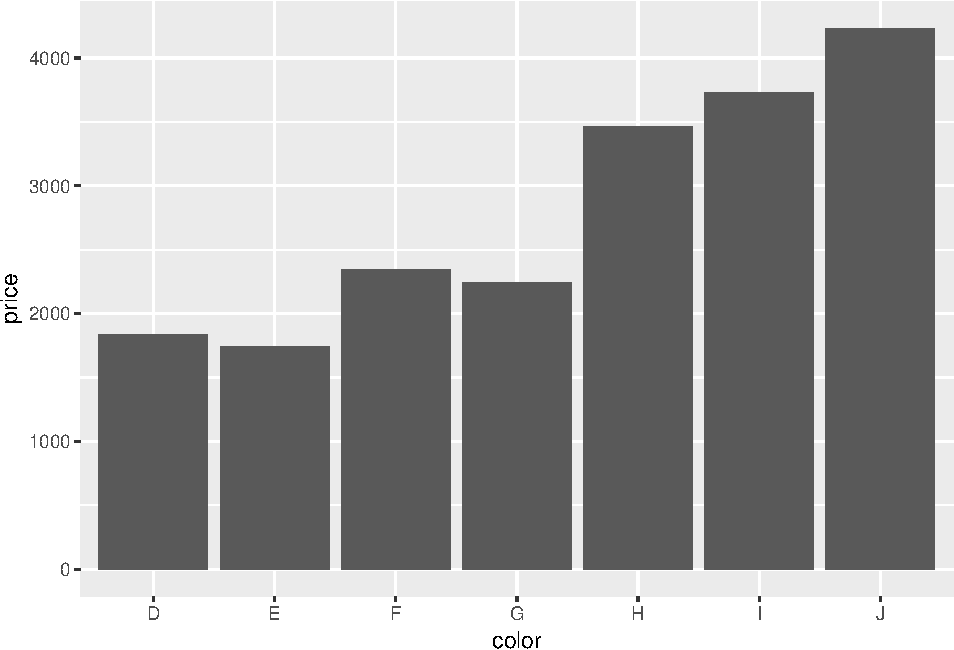
\includegraphics{02-visualization1_files/figure-latex/visualization1-25-1.pdf}

And instead of making a bar plot, we could plot some points.

\begin{Shaded}
\begin{Highlighting}[]
\KeywordTok{ggplot}\NormalTok{(df.diamonds, }\KeywordTok{aes}\NormalTok{(}\DataTypeTok{x =}\NormalTok{ color, }\DataTypeTok{y =}\NormalTok{ price)) }\OperatorTok{+}
\StringTok{  }\KeywordTok{stat_summary}\NormalTok{(}\DataTypeTok{fun.y =} \StringTok{"mean"}\NormalTok{, }\DataTypeTok{geom =} \StringTok{"point"}\NormalTok{)}
\end{Highlighting}
\end{Shaded}

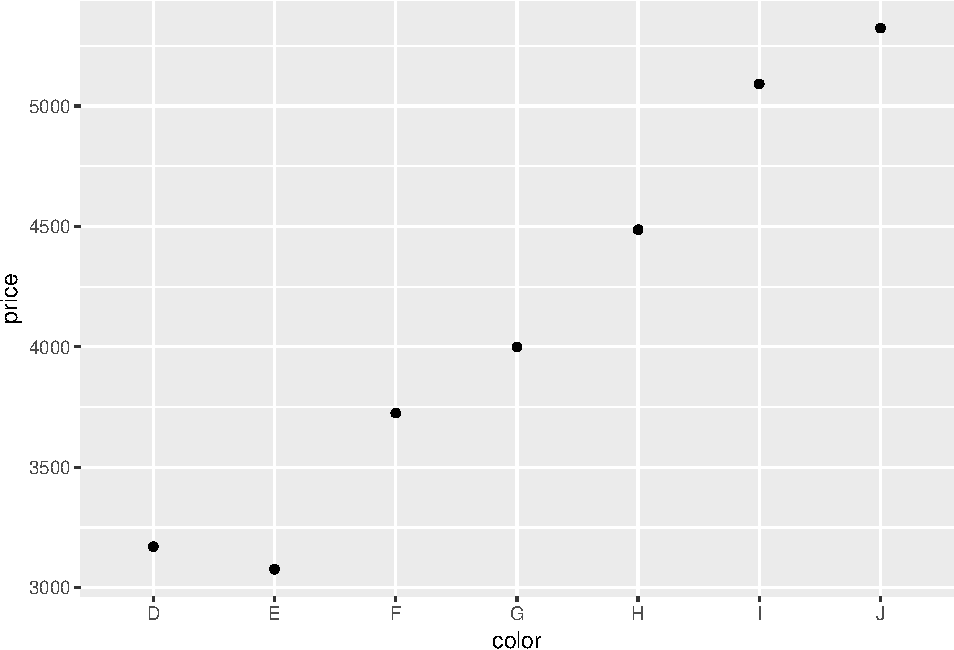
\includegraphics{02-visualization1_files/figure-latex/visualization1-26-1.pdf}

\begin{quote}
\textbf{Tip}: Take a look \href{https://ggplot2.tidyverse.org/reference/\#section-layer-geoms}{here} to see what other geoms ggplot2 supports.
\end{quote}

Somewhat surprisingly, diamonds with the best color (D) are not the most expensive ones. What's going on here? We'll need to do some more exploration to figure this out.

Note that in the last plot, I removed the \texttt{data\ =} and \texttt{mapping\ =} specifiers. These keywords are optional, and as long as we provide the arguments to the function in the correct order, we are ok. So, the following doesn't work:

\begin{Shaded}
\begin{Highlighting}[]
\KeywordTok{ggplot}\NormalTok{(}\KeywordTok{aes}\NormalTok{(}\DataTypeTok{x =}\NormalTok{ color, }\DataTypeTok{y =}\NormalTok{ price), df.diamonds) }\OperatorTok{+}
\StringTok{  }\KeywordTok{stat_summary}\NormalTok{(}\DataTypeTok{fun.y =} \StringTok{"mean"}\NormalTok{, }\DataTypeTok{geom =} \StringTok{"point"}\NormalTok{)}
\end{Highlighting}
\end{Shaded}

While this works:

\begin{Shaded}
\begin{Highlighting}[]
\KeywordTok{ggplot}\NormalTok{(}\DataTypeTok{mapping =} \KeywordTok{aes}\NormalTok{(}\DataTypeTok{x =}\NormalTok{ color, }\DataTypeTok{y =}\NormalTok{ price), }\DataTypeTok{data =}\NormalTok{ df.diamonds) }\OperatorTok{+}
\StringTok{  }\KeywordTok{stat_summary}\NormalTok{(}\DataTypeTok{fun.y =} \StringTok{"mean"}\NormalTok{, }\DataTypeTok{geom =} \StringTok{"point"}\NormalTok{)}
\end{Highlighting}
\end{Shaded}

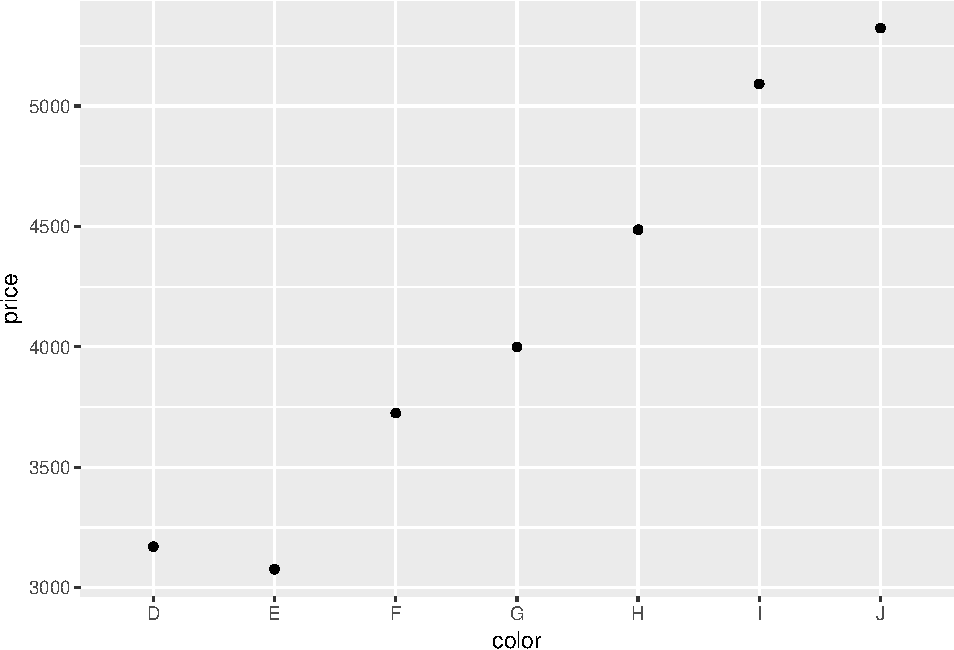
\includegraphics{02-visualization1_files/figure-latex/visualization1-28-1.pdf}

In general, it's good practice to include the specifiers -- particularly for functions that are not used all the time. If the same function is used multiple times throughout the script, I would suggest to use the specifiers first, and then it's ok to drop them later.

\hypertarget{setting-the-default-plot-theme}{%
\subsection{Setting the default plot theme}\label{setting-the-default-plot-theme}}

Before moving one, let's set a different default theme for our plots. Personally, I'm not a big fan of the gray background and the white grid lines. Also, the default size of the text should be bigger. We can change the default theme using the \texttt{theme\_set()} function like so:

\begin{Shaded}
\begin{Highlighting}[]
\KeywordTok{theme_set}\NormalTok{(}
  \KeywordTok{theme_classic}\NormalTok{() }\OperatorTok{+}\StringTok{ }\CommentTok{# set the theme}
\StringTok{    }\KeywordTok{theme}\NormalTok{(}\DataTypeTok{text =} \KeywordTok{element_text}\NormalTok{(}\DataTypeTok{size =} \DecValTok{20}\NormalTok{)) }\CommentTok{# set the default text size}
\NormalTok{)}
\end{Highlighting}
\end{Shaded}

From now onwards, all our plots will use what's specified in \texttt{theme\_classic()}, and the default text size will be larger, too. For any individual plot, we can still override these settings.

\hypertarget{scatter-plot}{%
\subsection{Scatter plot}\label{scatter-plot}}

I don't know much about diamonds, but I do know that diamonds with a higher \texttt{carat} value tend to be more expensive. \texttt{color} was a discrete variable with seven different values. \texttt{carat}, however, is a continuous variable. We want to see how the price of diamonds differs as a function of the \texttt{carat} value. Since we are interested in the relationship between two continuous variables, plotting a bar graph won't work. Instead, let's make a \textbf{scatter plot}. Let's put the \texttt{carat} value on the x-axis, and the \texttt{price} on the y-axis.

\begin{Shaded}
\begin{Highlighting}[]
\KeywordTok{ggplot}\NormalTok{(}\DataTypeTok{data =}\NormalTok{ df.diamonds, }\DataTypeTok{mapping =} \KeywordTok{aes}\NormalTok{(}\DataTypeTok{x =}\NormalTok{ carat, }\DataTypeTok{y =}\NormalTok{ price)) }\OperatorTok{+}
\StringTok{  }\KeywordTok{geom_point}\NormalTok{()}
\end{Highlighting}
\end{Shaded}

\begin{figure}
\centering
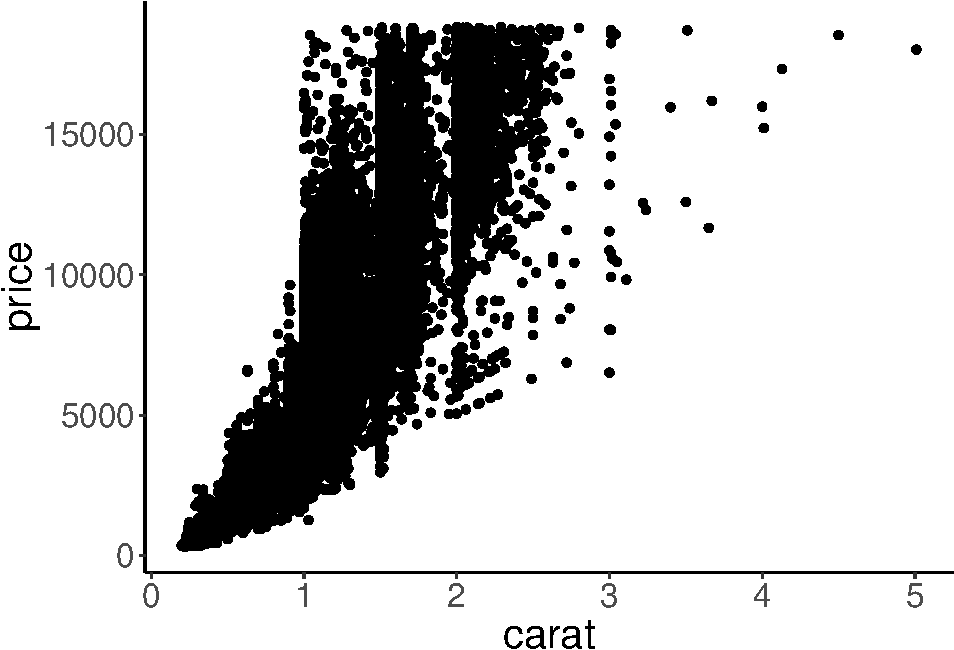
\includegraphics{02-visualization1_files/figure-latex/visualization1-30-1.pdf}
\caption{\label{fig:visualization1-30}Scatterplot.}
\end{figure}

Cool! That looks sensible. Diamonds with a higher \texttt{carat} value tend to have a higher \texttt{price}. Our dataset has 53940 rows. So the plot actually shows 53940 circles even though we can't see all of them since they overlap.

Let's make some progress on trying to figure out why the diamonds with the better color weren't the most expensive ones on average. We'll add some color to the scatter plot in Figure \ref{fig:visualization-31}. We color each of the points based on the diamond's color. To do so, we pass another argument to the aesthetics of the plot via \texttt{aes()}.

\begin{Shaded}
\begin{Highlighting}[]
\KeywordTok{ggplot}\NormalTok{(}\DataTypeTok{data =}\NormalTok{ df.diamonds,}
       \DataTypeTok{mapping =} \KeywordTok{aes}\NormalTok{(}\DataTypeTok{x =}\NormalTok{ carat,}
                     \DataTypeTok{y =}\NormalTok{ price,}
                     \DataTypeTok{color =}\NormalTok{ color)) }\OperatorTok{+}
\StringTok{  }\KeywordTok{geom_point}\NormalTok{()}
\end{Highlighting}
\end{Shaded}

\begin{figure}
\centering
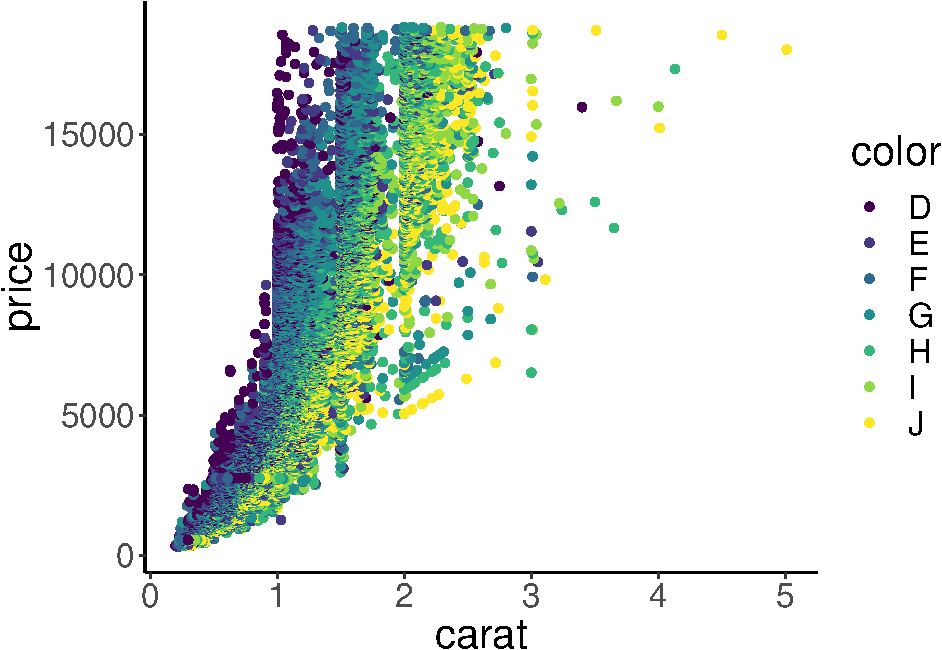
\includegraphics{02-visualization1_files/figure-latex/visualization1-31-1.pdf}
\caption{\label{fig:visualization1-31}Scatterplot with color.}
\end{figure}

Aha! Now we've got some color. Notice how in Figure \ref{fig:visualization-30} \texttt{ggplot2} added a legend for us, thanks! We'll see later how to play around with legends. Form just eye-balling the plot, it looks like the diamonds with the best \texttt{color} (D) tended to have a lower \texttt{carat} value, and the ones with the worst \texttt{color} (J), tended to have the highest carat values.

So this is why diamonds with better colors are less expensive -- these diamonds have a lower carat value overall.

There are many other things that we can define in \texttt{aes()}. Take a quick look at the vignette:

\begin{Shaded}
\begin{Highlighting}[]
\KeywordTok{vignette}\NormalTok{(}\StringTok{"ggplot2-specs"}\NormalTok{)}
\end{Highlighting}
\end{Shaded}

\hypertarget{practice-plot-1}{%
\subsubsection{Practice plot 1}\label{practice-plot-1}}

Make a scatter plot that shows the relationship between the variables \texttt{depth} (on the x-axis), and \texttt{table} (on the y-axis). Take a look at the description for the \texttt{diamonds} dataset so you know what these different variables mean. Your plot should look like the one shown in Figure \ref{fig:visualization1-34}.

\begin{Shaded}
\begin{Highlighting}[]
\CommentTok{# make practice plot 1 here}
\end{Highlighting}
\end{Shaded}

\begin{Shaded}
\begin{Highlighting}[]
\KeywordTok{include_graphics}\NormalTok{(}\StringTok{"figures/practice_plot1.png"}\NormalTok{)}
\end{Highlighting}
\end{Shaded}

\begin{figure}

{\centering 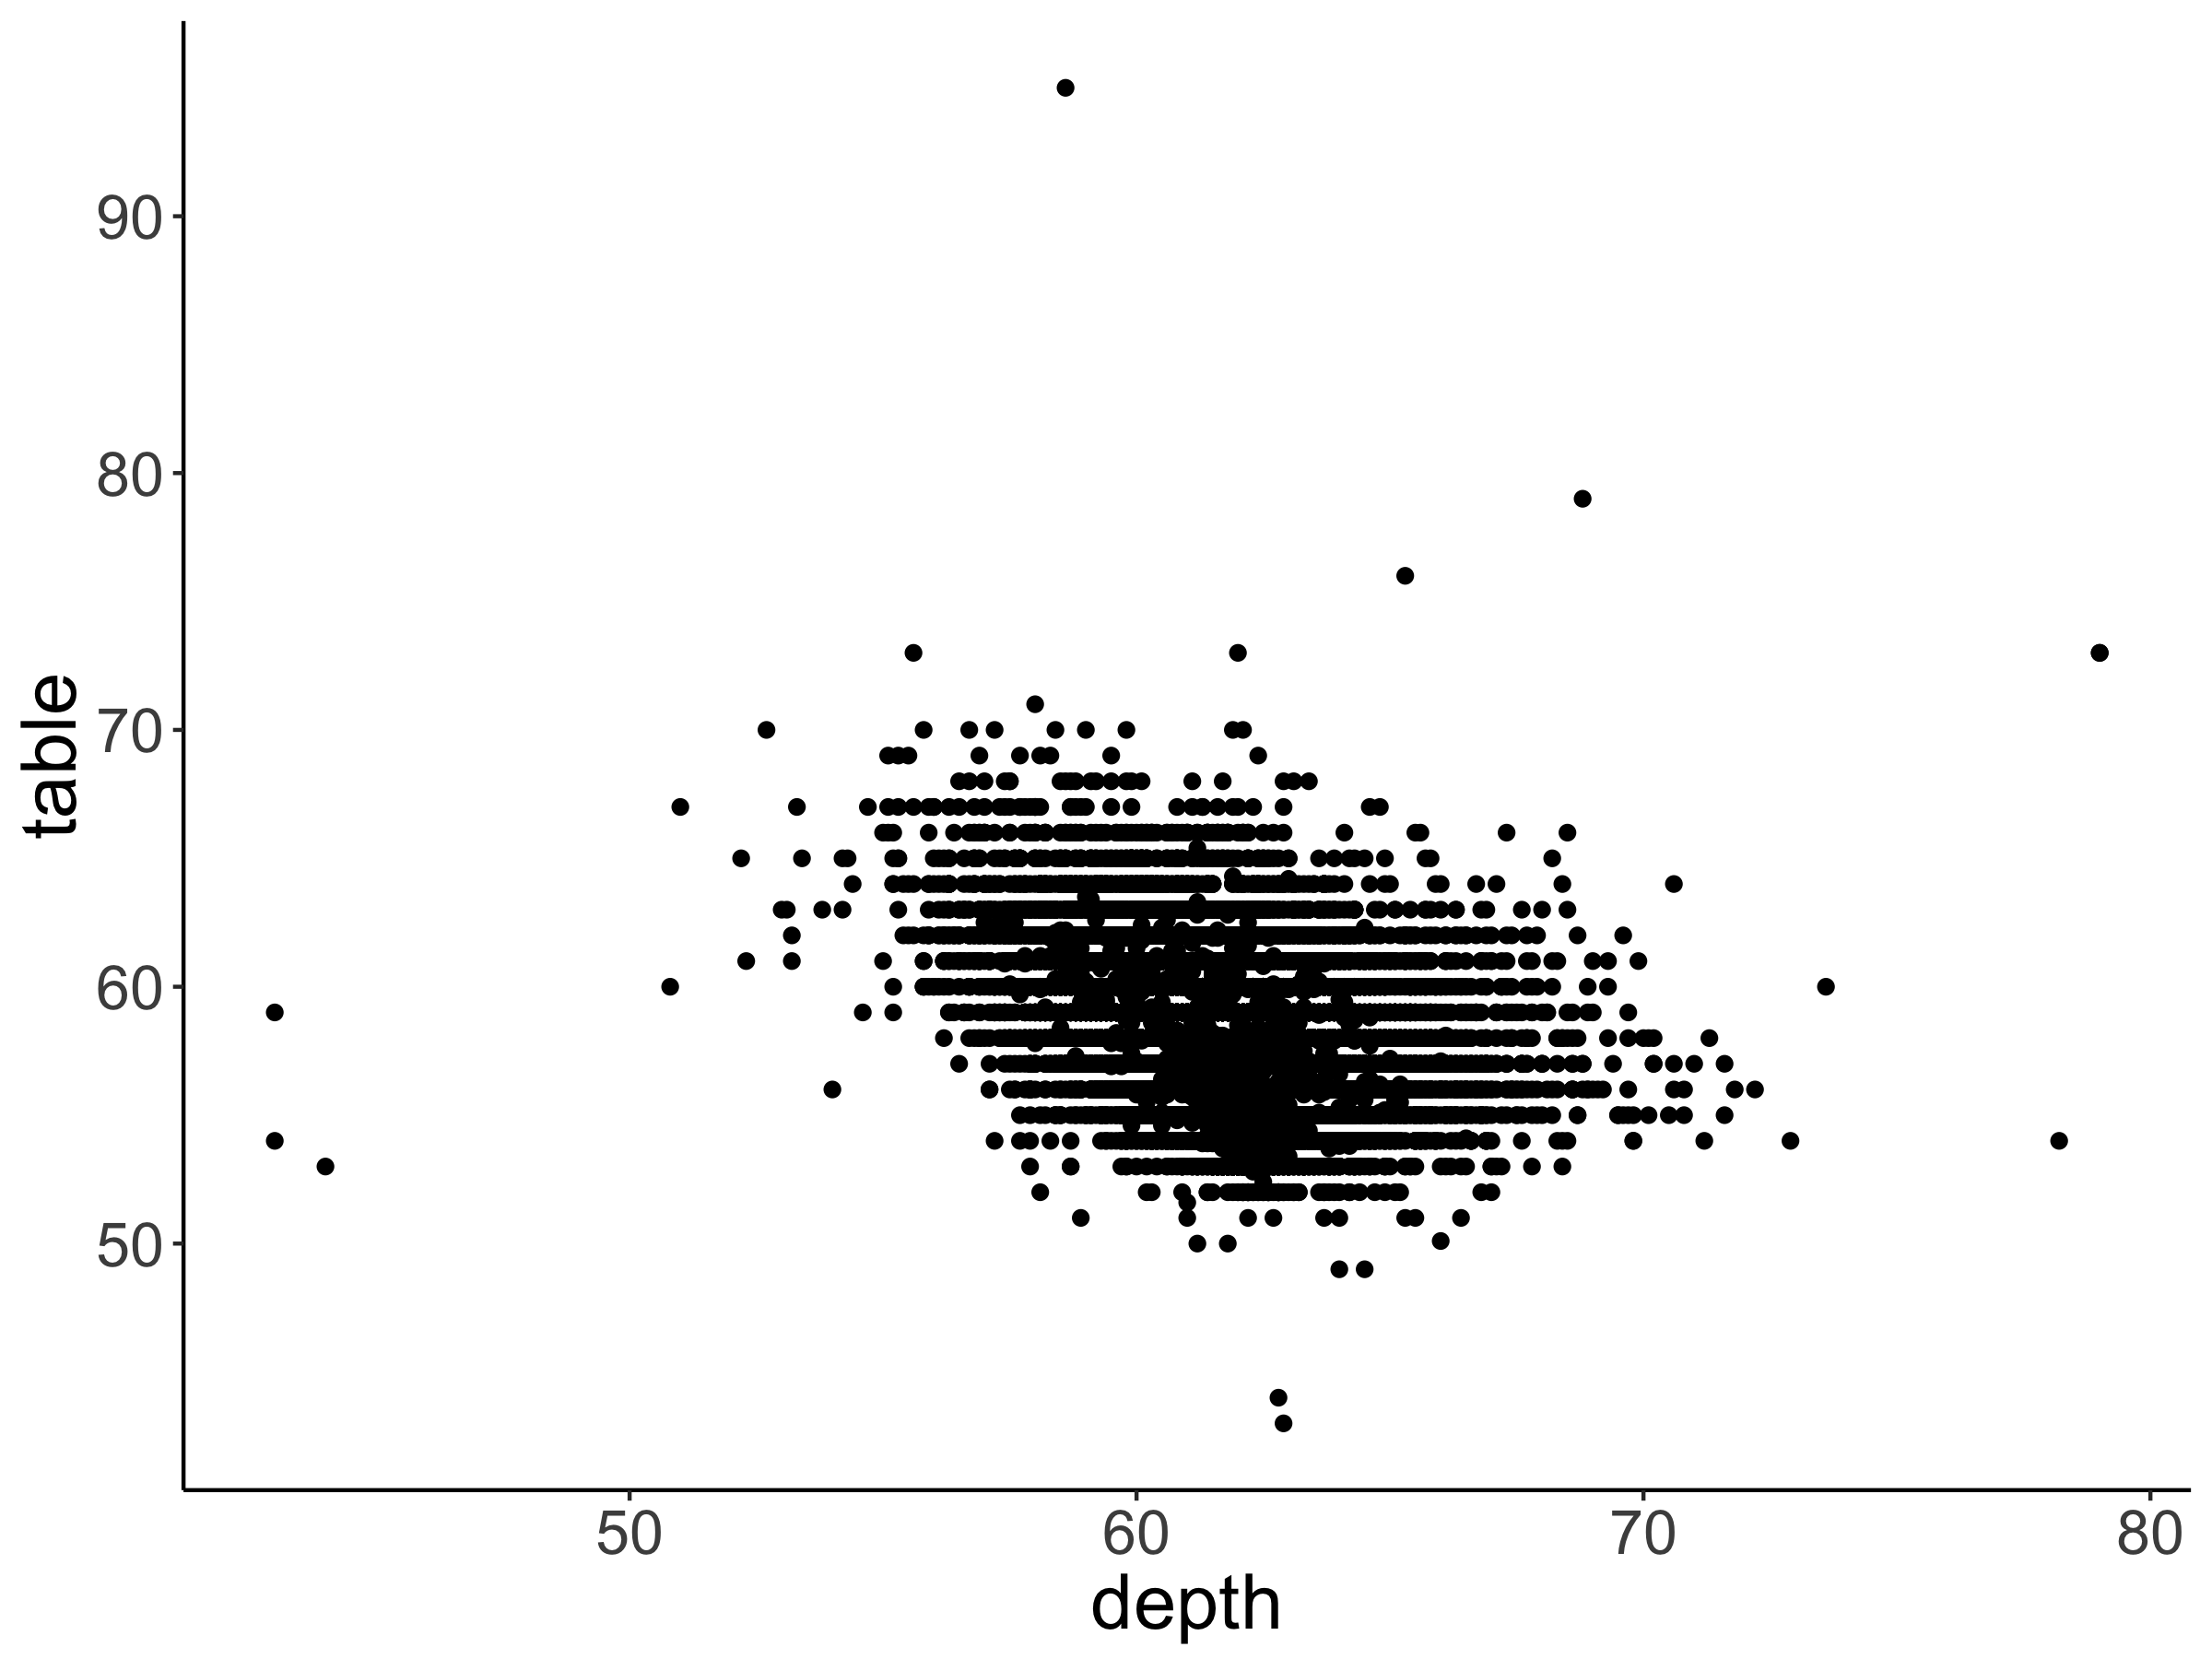
\includegraphics[width=0.9\linewidth]{figures/practice_plot1} 

}

\caption{Practice plot 1.}\label{fig:visualization1-34}
\end{figure}

\hypertarget{line-plot}{%
\subsection{Line plot}\label{line-plot}}

What else do we know about the diamonds? We actually know the quality of how they were cut. The \texttt{cut} variable ranges from ``Fair'' to ``Ideal''. First, let's take a look at the relationship between \texttt{cut} and \texttt{price}. This time, we'll make a line plot instead of a bar plot (just because we can).

\begin{Shaded}
\begin{Highlighting}[]
\KeywordTok{ggplot}\NormalTok{(}\DataTypeTok{data =}\NormalTok{ df.diamonds, }\DataTypeTok{mapping =} \KeywordTok{aes}\NormalTok{(}\DataTypeTok{x =}\NormalTok{ cut, }\DataTypeTok{y =}\NormalTok{ price)) }\OperatorTok{+}
\StringTok{  }\KeywordTok{stat_summary}\NormalTok{(}\DataTypeTok{fun.y =} \StringTok{"mean"}\NormalTok{, }\DataTypeTok{geom =} \StringTok{"line"}\NormalTok{)}
\end{Highlighting}
\end{Shaded}

\begin{verbatim}
## geom_path: Each group consists of only one observation. Do you need to
## adjust the group aesthetic?
\end{verbatim}

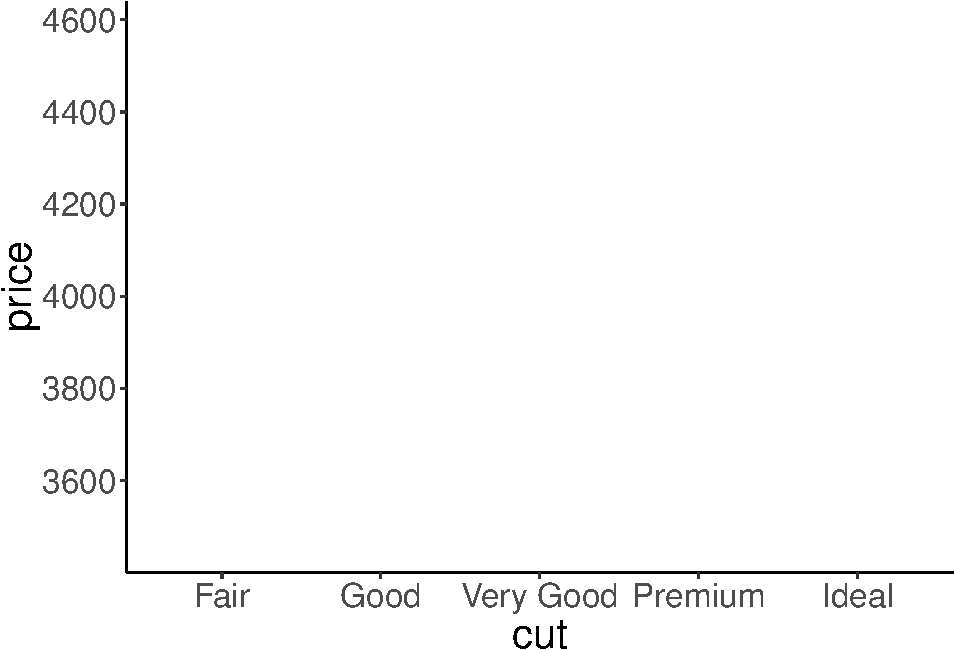
\includegraphics{02-visualization1_files/figure-latex/visualization1-35-1.pdf}

Oops! All we did is that we replaced \texttt{x\ =\ color} with \texttt{x\ =\ cut}, and \texttt{geom\ =\ "bar"} with \texttt{geom\ =\ "line"}. However, the plot doesn't look like expected (i.e.~there is no real plot). What happened here? The reason is that the line plot needs to know what points to connect. The error message tells us that each group consists of only one observation. Let's adjust the group asthetic to fix this.

\begin{Shaded}
\begin{Highlighting}[]
\KeywordTok{ggplot}\NormalTok{(}\DataTypeTok{data =}\NormalTok{ df.diamonds, }\DataTypeTok{mapping =} \KeywordTok{aes}\NormalTok{(}\DataTypeTok{x =}\NormalTok{ cut, }\DataTypeTok{y =}\NormalTok{ price, }\DataTypeTok{group =} \DecValTok{1}\NormalTok{)) }\OperatorTok{+}
\StringTok{  }\KeywordTok{stat_summary}\NormalTok{(}\DataTypeTok{fun.y =} \StringTok{"mean"}\NormalTok{, }\DataTypeTok{geom =} \StringTok{"line"}\NormalTok{)}
\end{Highlighting}
\end{Shaded}

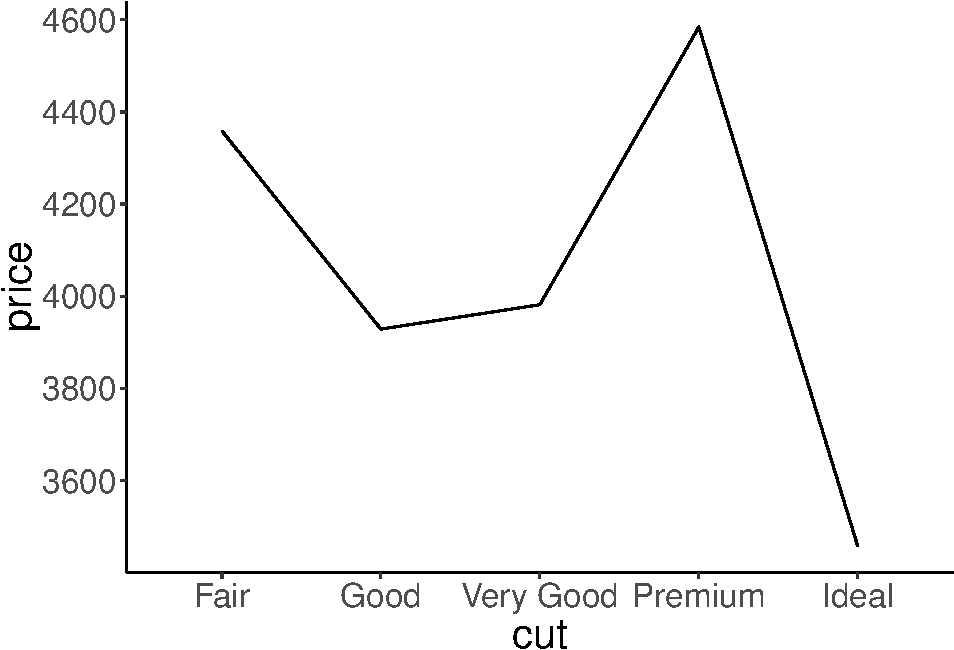
\includegraphics{02-visualization1_files/figure-latex/visualization1-36-1.pdf}

By adding the parameter \texttt{group\ =\ 1} to \texttt{mapping\ =\ aes()}, we specify that we would like all the levels in \texttt{x\ =\ cut} to be treated as coming from the same group. The reason for this is that \texttt{cut} (our x-axis variable) is a factor (and not a numeric variable), so, by default, \texttt{ggplot2} tries to draw a separate line for each factor level. We'll learn more about grouping below (and about factors later).

Interestingly, there is no simple relationship between the quality of the cut and the price of the diamond. In fact, ``Ideal'' diamonds tend to be cheapest.

\hypertarget{adding-error-bars}{%
\subsection{Adding error bars}\label{adding-error-bars}}

We often don't just want to show the means but also give a sense for how much the data varies. \texttt{ggplot2} has some convenient ways of specifying error bars. Let's take a look at how much \texttt{price} varies as a function of \texttt{clarity} (another variable in our \texttt{diamonds} data frame).

\begin{Shaded}
\begin{Highlighting}[]
\KeywordTok{ggplot}\NormalTok{(}\DataTypeTok{data =}\NormalTok{ df.diamonds,}
       \DataTypeTok{mapping =} \KeywordTok{aes}\NormalTok{(}\DataTypeTok{x =}\NormalTok{ clarity, }\DataTypeTok{y =}\NormalTok{ price)) }\OperatorTok{+}
\StringTok{  }\KeywordTok{stat_summary}\NormalTok{(}\DataTypeTok{fun.data =} \StringTok{"mean_cl_boot"}\NormalTok{,}
               \DataTypeTok{geom =} \StringTok{"linerange"}\NormalTok{) }\OperatorTok{+}\StringTok{ }\CommentTok{# plot bootstrapped error bars first}
\StringTok{  }\KeywordTok{stat_summary}\NormalTok{(}\DataTypeTok{fun.y =} \StringTok{"mean"}\NormalTok{,}
               \DataTypeTok{geom =} \StringTok{"point"}\NormalTok{) }\CommentTok{# add points with means}
\end{Highlighting}
\end{Shaded}

\begin{figure}
\centering
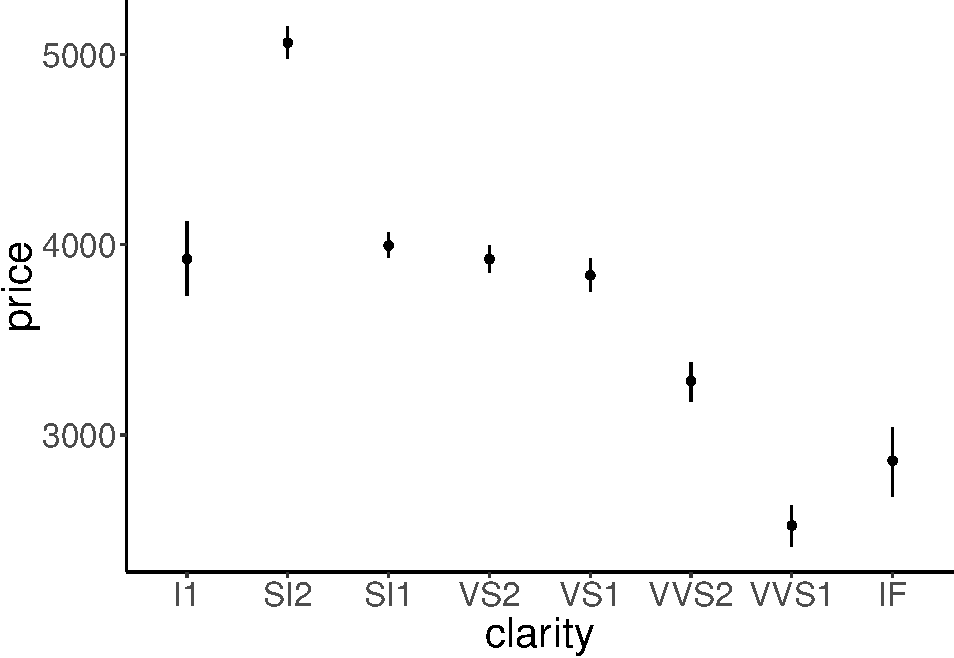
\includegraphics{02-visualization1_files/figure-latex/visualization1-37-1.pdf}
\caption{\label{fig:visualization1-37}Relationship between diamond clarity and price. Error bars indicate 95\% bootstrapped confidence intervals.}
\end{figure}

Here we have it. The average price of our diamonds for different levels of \texttt{clarity} together with bootstrapped 95\% confidence intervals. How do we know that we have 95\% confidence intervals? That's what \texttt{mean\_cl\_boot()} computes as a default. Let's take a look at that function:

\begin{Shaded}
\begin{Highlighting}[]
\KeywordTok{help}\NormalTok{(mean_cl_boot)}
\end{Highlighting}
\end{Shaded}

Remember that you can just select the text (or merely put the cursor over the word) and press \texttt{F1} to see the help. The help file tell us about the function \texttt{smean.cl.boot} in the \texttt{Hmisc} package. The \texttt{mean\_cl\_boot()} function is a version that works well with \texttt{ggplot2}. We see that this function takes as inputs, the confidence interval \texttt{conf.int}, the number of bootstrap samples \texttt{B}, and some other ones that we don't care about for now. So let's make the same plot again with 99.9\% confidence intervals, and 2000 bootstrap samples.

\begin{Shaded}
\begin{Highlighting}[]
\KeywordTok{ggplot}\NormalTok{(}\DataTypeTok{data =}\NormalTok{ df.diamonds, }\DataTypeTok{mapping =} \KeywordTok{aes}\NormalTok{(}\DataTypeTok{x =}\NormalTok{ clarity, }\DataTypeTok{y =}\NormalTok{ price)) }\OperatorTok{+}
\StringTok{  }\KeywordTok{stat_summary}\NormalTok{(}\DataTypeTok{fun.data =} \StringTok{"mean_cl_boot"}\NormalTok{,}
               \DataTypeTok{geom =} \StringTok{"linerange"}\NormalTok{,}
               \DataTypeTok{fun.args =} \KeywordTok{list}\NormalTok{(}\DataTypeTok{conf.int =} \FloatTok{.999}\NormalTok{, }\DataTypeTok{B =} \DecValTok{2000}\NormalTok{)) }\OperatorTok{+}\StringTok{ }\CommentTok{# plot bootstrapped error bars first}
\StringTok{  }\KeywordTok{stat_summary}\NormalTok{(}\DataTypeTok{fun.y =} \StringTok{"mean"}\NormalTok{,}
               \DataTypeTok{geom =} \StringTok{"point"}\NormalTok{) }\CommentTok{# add points with means}
\end{Highlighting}
\end{Shaded}

\begin{figure}
\centering
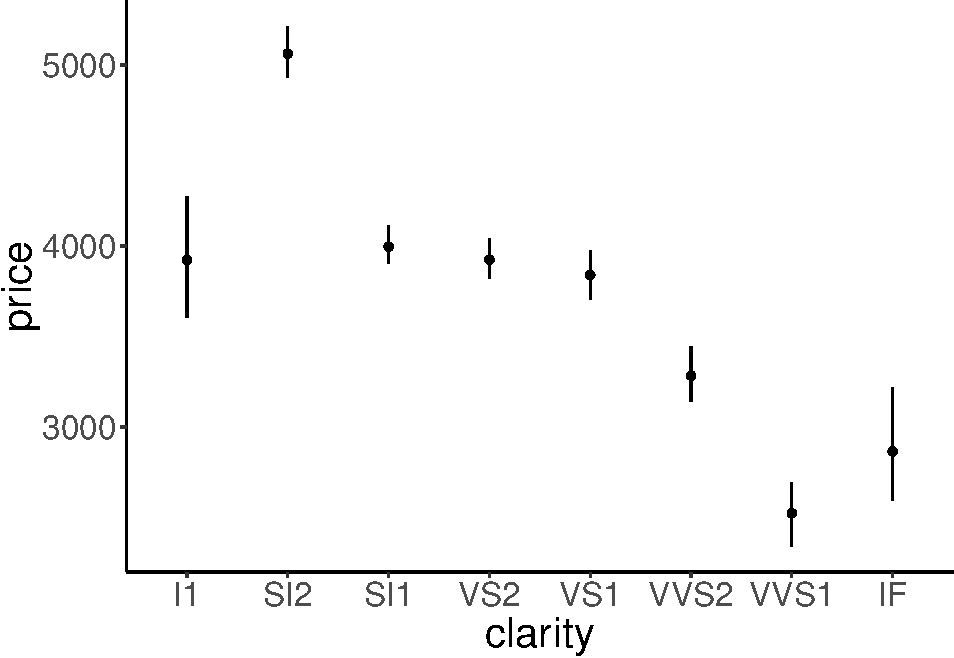
\includegraphics{02-visualization1_files/figure-latex/visualization1-39-1.pdf}
\caption{\label{fig:visualization1-39}Relationship between diamond clarity and price. Error bars indicate 99\% bootstrapped confidence intervals.}
\end{figure}

Note how the error bars are larger now in Figure Figure \ref{fig:visualization-39} compared to Figure \ref{fig:visualization-37}
. Note the somewhat peculiar way in which we supplied the parameters to the \texttt{mean\_cl\_boot} function. The \texttt{fun.args} argument takes in a list of arguments that it then passes on to the function \texttt{mean\_cl\_boot}.

\hypertarget{order-matters}{%
\subsubsection{Order matters}\label{order-matters}}

The order in which we add geoms to a ggplot matters! Generally, we want to plot error bars before the points that represent the means. To illustrate, let's set the color in which we show the means to ``red''.

\begin{Shaded}
\begin{Highlighting}[]
\KeywordTok{ggplot}\NormalTok{(df.diamonds, }\KeywordTok{aes}\NormalTok{(}\DataTypeTok{x =}\NormalTok{ clarity, }\DataTypeTok{y =}\NormalTok{ price)) }\OperatorTok{+}
\StringTok{  }\KeywordTok{stat_summary}\NormalTok{(}\DataTypeTok{fun.data =} \StringTok{"mean_cl_boot"}\NormalTok{, }\DataTypeTok{geom =} \StringTok{"linerange"}\NormalTok{) }\OperatorTok{+}
\StringTok{  }\KeywordTok{stat_summary}\NormalTok{(}\DataTypeTok{fun.y =} \StringTok{"mean"}\NormalTok{, }\DataTypeTok{geom =} \StringTok{"point"}\NormalTok{, }\DataTypeTok{color =} \StringTok{"red"}\NormalTok{)}
\end{Highlighting}
\end{Shaded}

\begin{figure}
\centering
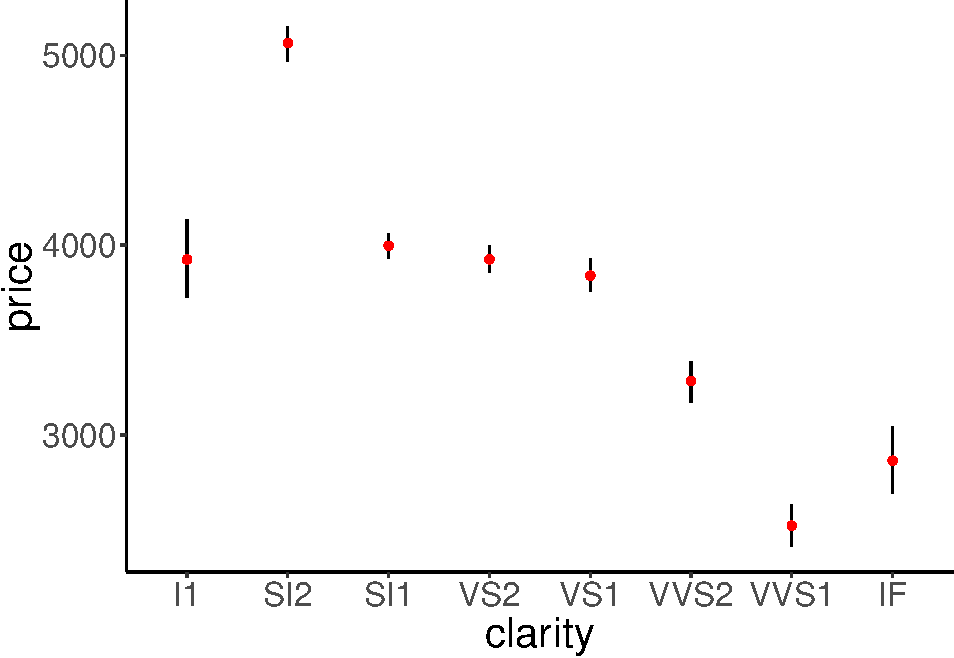
\includegraphics{02-visualization1_files/figure-latex/visualization1-40-1.pdf}
\caption{\label{fig:visualization1-40}This figure looks good. Error bars and means are drawn in the correct order.}
\end{figure}

Figure \ref{fig:visualization-38} looks good.

\begin{Shaded}
\begin{Highlighting}[]
\CommentTok{# I've changed the order in which the means and error bars are drawn.}
\KeywordTok{ggplot}\NormalTok{(df.diamonds, }\KeywordTok{aes}\NormalTok{(}\DataTypeTok{x =}\NormalTok{ clarity, }\DataTypeTok{y =}\NormalTok{ price)) }\OperatorTok{+}
\StringTok{  }\KeywordTok{stat_summary}\NormalTok{(}\DataTypeTok{fun.y =} \StringTok{"mean"}\NormalTok{, }\DataTypeTok{geom =} \StringTok{"point"}\NormalTok{, }\DataTypeTok{color =} \StringTok{"red"}\NormalTok{) }\OperatorTok{+}
\StringTok{  }\KeywordTok{stat_summary}\NormalTok{(}\DataTypeTok{fun.data =} \StringTok{"mean_cl_boot"}\NormalTok{, }\DataTypeTok{geom =} \StringTok{"linerange"}\NormalTok{)}
\end{Highlighting}
\end{Shaded}

\begin{figure}
\centering
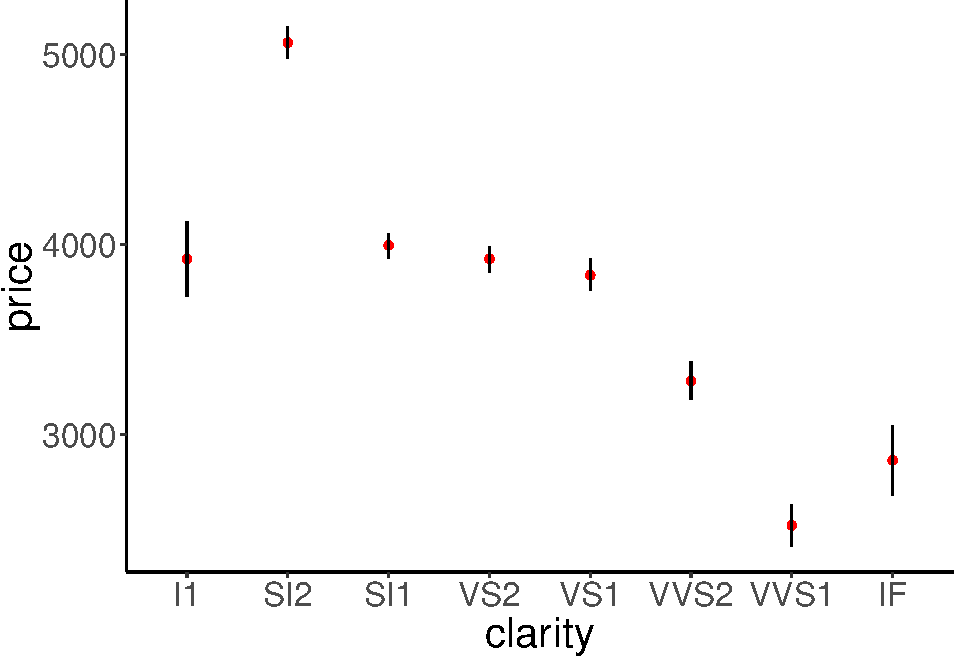
\includegraphics{02-visualization1_files/figure-latex/visualization1-41-1.pdf}
\caption{\label{fig:visualization1-41}This figure looks good. Error bars and means are drawn in the correct order.}
\end{figure}

Figure \ref{fig:visualization-39} doesn't look good. The error bars are on top of the points that represent the means.

One cool feature about using \texttt{stat\_summary()} is that we did not have to change anything about the data frame that we used to make the plots. We directly used our raw data instead of having to make separate data frames that contain the relevant information (such as the means and the confidence intervals).

You may not remember exactly what confidence intervals actually are. Don't worry! We'll have a recap later in class.

Let's take a look at two more principles for plotting data that are extremely helpful: groups and facets. But before, another practice plot.

\hypertarget{practice-plot-2}{%
\subsubsection{Practice plot 2}\label{practice-plot-2}}

Make a bar plot that shows the average \texttt{price} of diamonds (on the y-axis) as a function of their \texttt{clarity} (on the x-axis). Also add error bars. Your plot should look like the one shown in Figure \ref{fig:visualization-41}.

\begin{Shaded}
\begin{Highlighting}[]
\CommentTok{# make practice plot 2 here}
\end{Highlighting}
\end{Shaded}

\begin{Shaded}
\begin{Highlighting}[]
\KeywordTok{include_graphics}\NormalTok{(}\StringTok{"figures/practice_plot2.png"}\NormalTok{)}
\end{Highlighting}
\end{Shaded}

\begin{figure}

{\centering 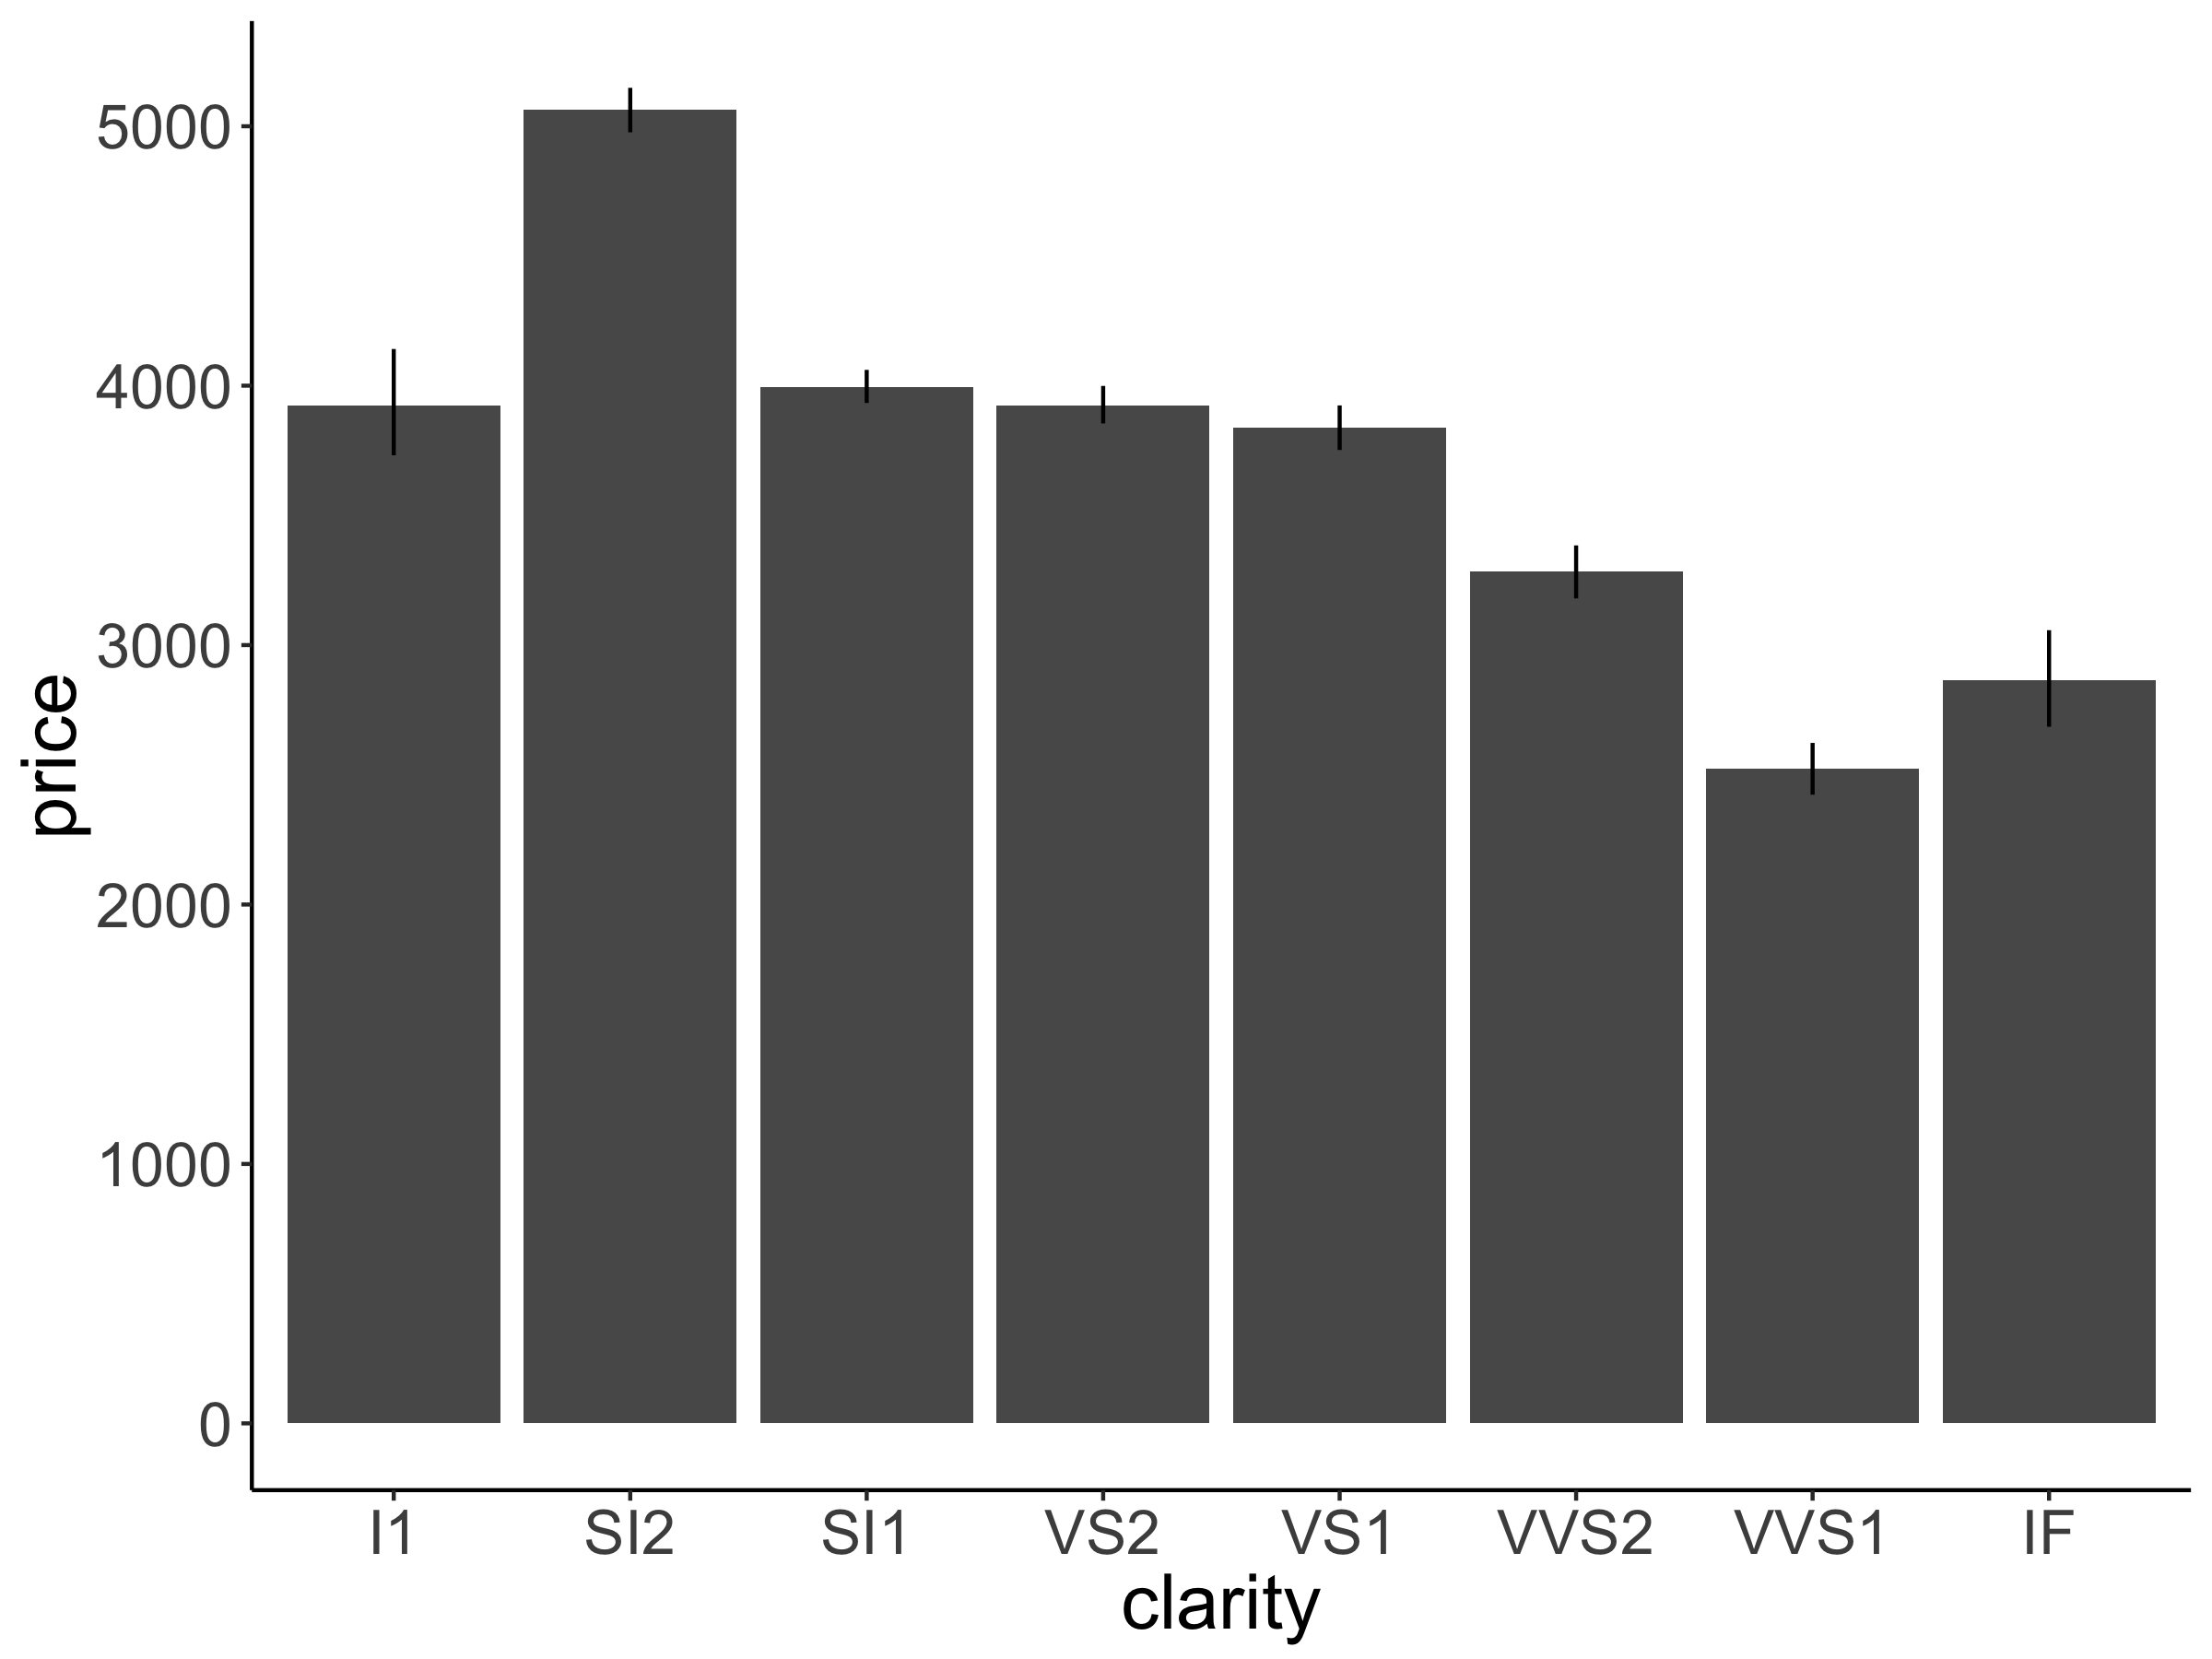
\includegraphics[width=0.9\linewidth]{figures/practice_plot2} 

}

\caption{Practice plot 2.}\label{fig:visualization1-43}
\end{figure}

\hypertarget{grouping-data}{%
\subsection{Grouping data}\label{grouping-data}}

Grouping in \texttt{ggplot2} is a very powerful idea. It allows us to plot subsets of the data -- again without the need to make separate data frames first.

Let's make a plot that shows the relationship between \texttt{price} and \texttt{color} separately for the different qualities of \texttt{cut}.

\begin{Shaded}
\begin{Highlighting}[]
\KeywordTok{ggplot}\NormalTok{(}\DataTypeTok{data =}\NormalTok{ df.diamonds,}
       \DataTypeTok{mapping =} \KeywordTok{aes}\NormalTok{(}\DataTypeTok{x =}\NormalTok{ color,}
                     \DataTypeTok{y =}\NormalTok{ price,}
                     \DataTypeTok{group =}\NormalTok{ cut)) }\OperatorTok{+}
\StringTok{  }\KeywordTok{stat_summary}\NormalTok{(}\DataTypeTok{fun.y =} \StringTok{"mean"}\NormalTok{, }\DataTypeTok{geom =} \StringTok{"line"}\NormalTok{)}
\end{Highlighting}
\end{Shaded}

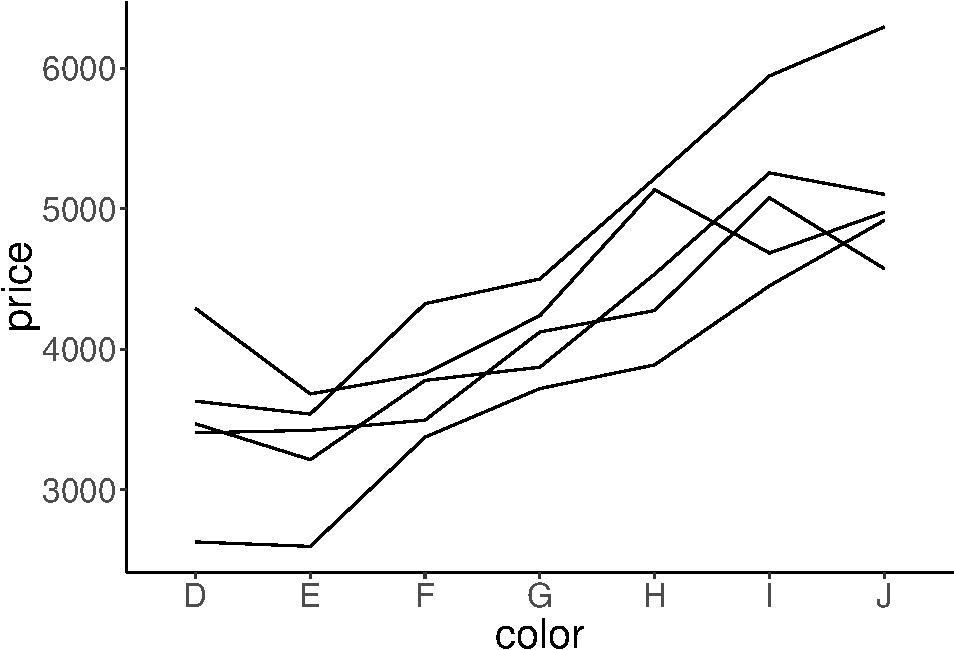
\includegraphics{02-visualization1_files/figure-latex/visualization1-44-1.pdf}

Well, we got some separate lines here but we don't know which line corresponds to which cut. Let's add some color!

\begin{Shaded}
\begin{Highlighting}[]
\KeywordTok{ggplot}\NormalTok{(}\DataTypeTok{data =}\NormalTok{ df.diamonds,}
       \DataTypeTok{mapping =} \KeywordTok{aes}\NormalTok{(}\DataTypeTok{x =}\NormalTok{ color,}
                     \DataTypeTok{y =}\NormalTok{ price,}
                     \DataTypeTok{group =}\NormalTok{ cut,}
                     \DataTypeTok{color =}\NormalTok{ cut)) }\OperatorTok{+}
\StringTok{  }\KeywordTok{stat_summary}\NormalTok{(}\DataTypeTok{fun.y =} \StringTok{"mean"}\NormalTok{,}
               \DataTypeTok{geom =} \StringTok{"line"}\NormalTok{,}
               \DataTypeTok{size =} \DecValTok{2}\NormalTok{)}
\end{Highlighting}
\end{Shaded}

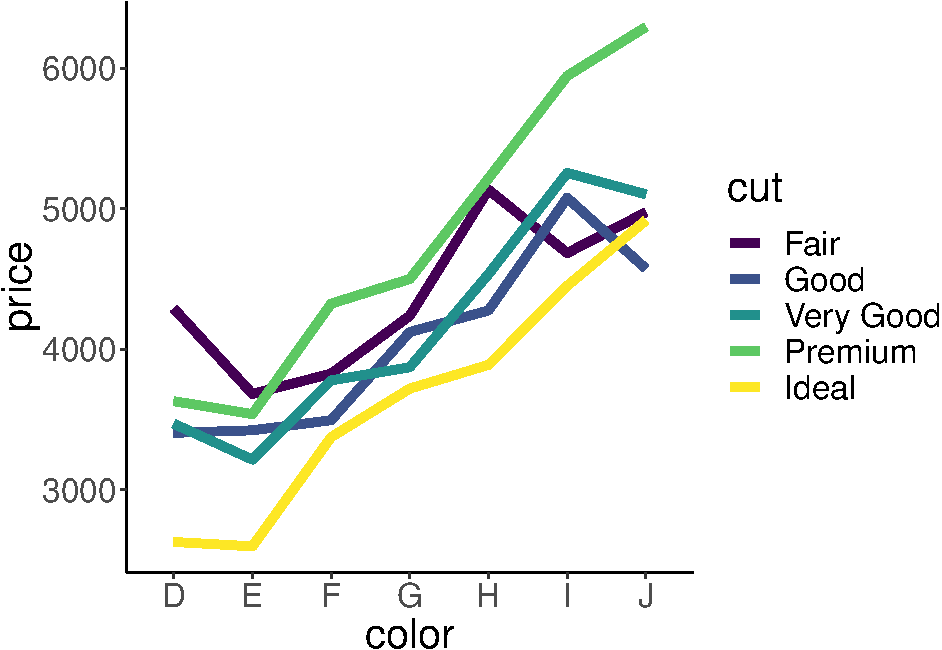
\includegraphics{02-visualization1_files/figure-latex/visualization1-45-1.pdf}

Nice! In addition to adding color, I've made the lines a little thicker here by setting the \texttt{size} argument to 2.

Grouping is very useful for bar plots. Let's take a look at how the average price of diamonds looks like taking into account both \texttt{cut} and \texttt{color} (I know -- exciting times!). Let's put the \texttt{color} on the x-axis and then group by the \texttt{cut}.

\begin{Shaded}
\begin{Highlighting}[]
\KeywordTok{ggplot}\NormalTok{(}\DataTypeTok{data =}\NormalTok{ df.diamonds,}
       \DataTypeTok{mapping =} \KeywordTok{aes}\NormalTok{(}\DataTypeTok{x =}\NormalTok{ color,}
                     \DataTypeTok{y =}\NormalTok{ price,}
                     \DataTypeTok{group =}\NormalTok{ cut,}
                     \DataTypeTok{color =}\NormalTok{ cut)) }\OperatorTok{+}
\StringTok{  }\KeywordTok{stat_summary}\NormalTok{(}\DataTypeTok{fun.y =} \StringTok{"mean"}\NormalTok{, }\DataTypeTok{geom =} \StringTok{"bar"}\NormalTok{)}
\end{Highlighting}
\end{Shaded}

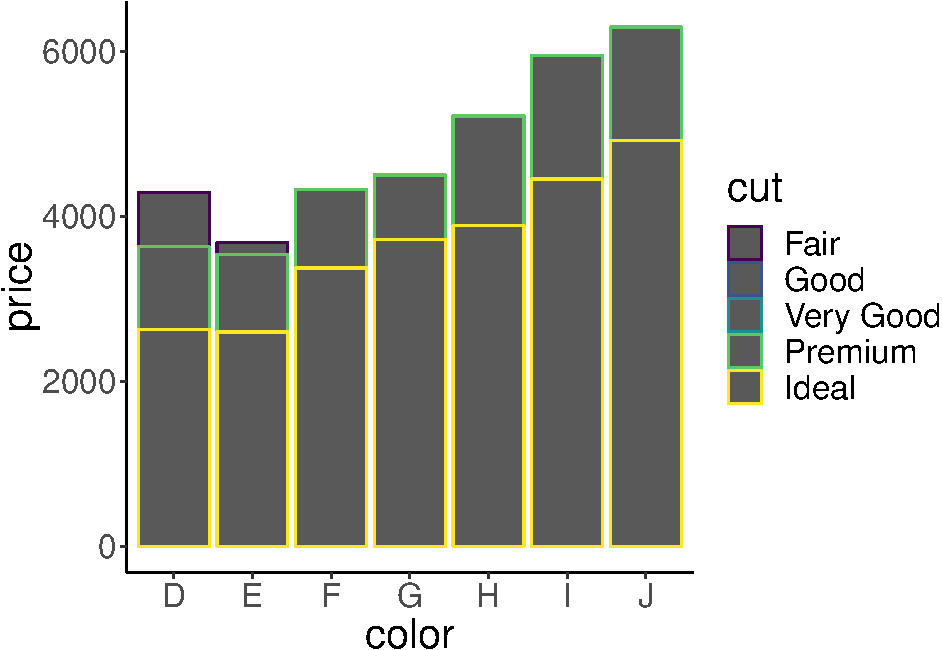
\includegraphics{02-visualization1_files/figure-latex/visualization1-46-1.pdf}

That's a fail! Several things went wrong here. All the bars are gray and only their outline is colored differently. Instead we want the bars to have a different color. For that we need to specify the \texttt{fill} argument rather than the \texttt{color} argument! But things are worse. The bars currently are shown on top of each other. Instead, we'd like to put them next to each other. Here is how we can do that:

\begin{Shaded}
\begin{Highlighting}[]
\KeywordTok{ggplot}\NormalTok{(}\DataTypeTok{data =}\NormalTok{ df.diamonds,}
       \DataTypeTok{mapping =} \KeywordTok{aes}\NormalTok{(}\DataTypeTok{x =}\NormalTok{ color,}
                     \DataTypeTok{y =}\NormalTok{ price,}
                     \DataTypeTok{group =}\NormalTok{ cut,}
                     \DataTypeTok{fill =}\NormalTok{ cut)) }\OperatorTok{+}
\StringTok{  }\KeywordTok{stat_summary}\NormalTok{(}\DataTypeTok{fun.y =} \StringTok{"mean"}\NormalTok{,}
               \DataTypeTok{geom =} \StringTok{"bar"}\NormalTok{,}
               \DataTypeTok{position =} \KeywordTok{position_dodge}\NormalTok{()) }\OperatorTok{+}
\StringTok{  }\KeywordTok{scale_fill_manual}\NormalTok{(}\DataTypeTok{values =} \KeywordTok{c}\NormalTok{(}\StringTok{"lightblue"}\NormalTok{, }\StringTok{"blue"}\NormalTok{, }\StringTok{"orangered"}\NormalTok{, }\StringTok{"red"}\NormalTok{, }\StringTok{"black"}\NormalTok{))}
\end{Highlighting}
\end{Shaded}

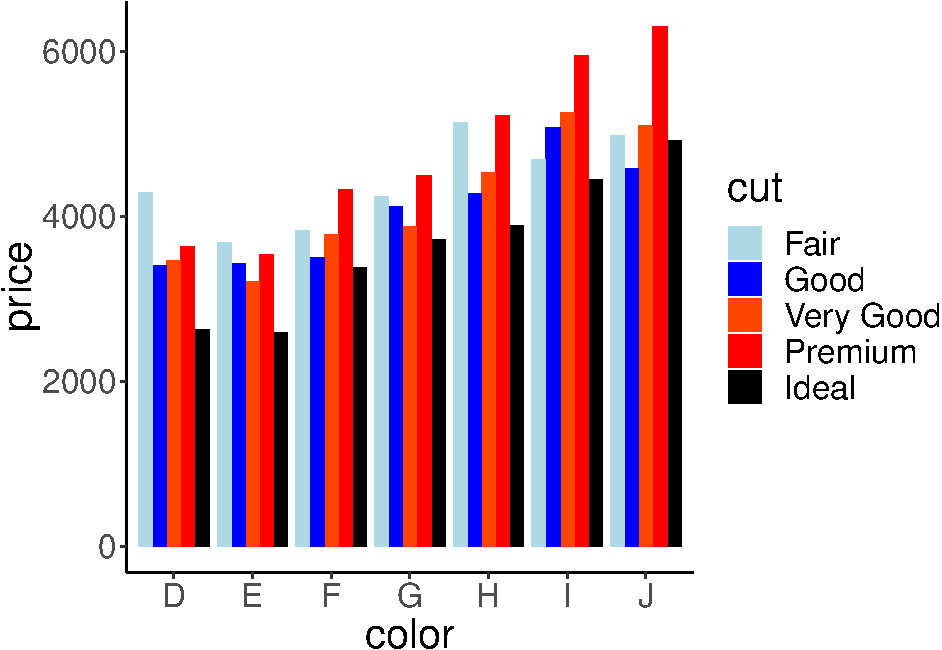
\includegraphics{02-visualization1_files/figure-latex/visualization1-47-1.pdf}

Neato! We've changed the \texttt{color} argument to \texttt{fill}, and have added the \texttt{position\ =\ position\_dodge()} argument to the \texttt{stat\_summary()} call. This argument makes it such that the bars are nicely dodged next to each other. Let's add some error bars just for kicks.

\begin{Shaded}
\begin{Highlighting}[]
\KeywordTok{ggplot}\NormalTok{(}\DataTypeTok{data =}\NormalTok{ df.diamonds,}
       \DataTypeTok{mapping =} \KeywordTok{aes}\NormalTok{(}\DataTypeTok{x =}\NormalTok{ color,}
                     \DataTypeTok{y =}\NormalTok{ price,}
                     \DataTypeTok{group =}\NormalTok{ cut,}
                     \DataTypeTok{fill =}\NormalTok{ cut)) }\OperatorTok{+}
\StringTok{  }\KeywordTok{stat_summary}\NormalTok{(}\DataTypeTok{fun.y =} \StringTok{"mean"}\NormalTok{,}
               \DataTypeTok{geom =} \StringTok{"bar"}\NormalTok{,}
               \DataTypeTok{position =} \KeywordTok{position_dodge}\NormalTok{(}\DataTypeTok{width =} \FloatTok{0.9}\NormalTok{),}
               \DataTypeTok{color =} \StringTok{"black"}\NormalTok{) }\OperatorTok{+}
\StringTok{  }\KeywordTok{stat_summary}\NormalTok{(}\DataTypeTok{fun.data =} \StringTok{"mean_cl_boot"}\NormalTok{,}
               \DataTypeTok{geom =} \StringTok{"linerange"}\NormalTok{,}
               \DataTypeTok{position =} \KeywordTok{position_dodge}\NormalTok{(}\DataTypeTok{width =} \FloatTok{0.9}\NormalTok{))}
\end{Highlighting}
\end{Shaded}

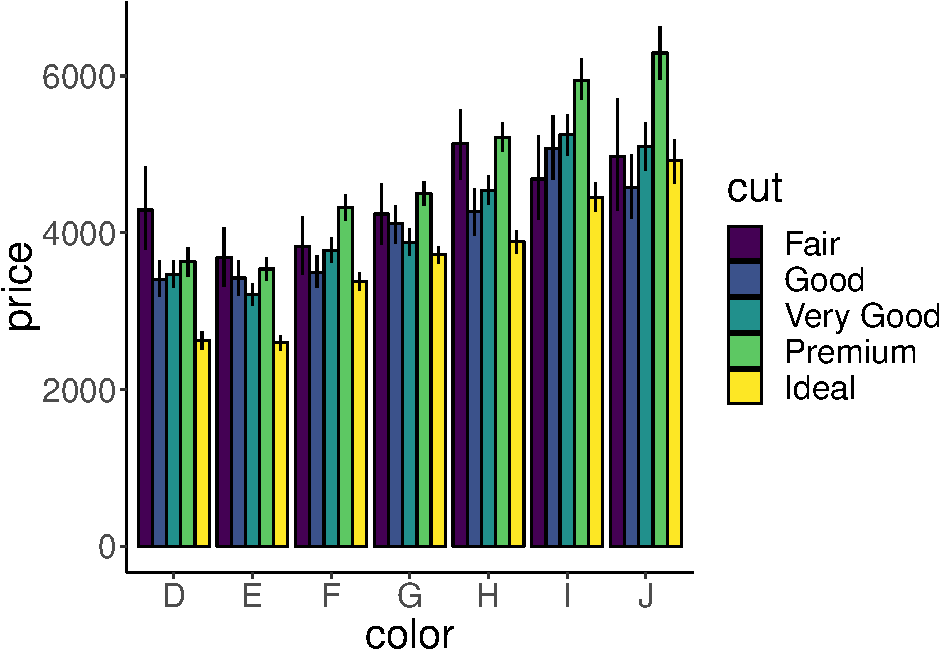
\includegraphics{02-visualization1_files/figure-latex/visualization1-48-1.pdf}

Voila! Now with error bars. Note that we've added the \texttt{width\ =\ 0.9} argument to \texttt{position\_dodge()}. Somehow R was complaining when this was not defined for geom ``linerange''. I've also added some outline to the bars by including the argument \texttt{color\ =\ "black"}. I think it looks nicer this way.

So, still somewhat surprisingly, diamonds with the worst color (J) are more expensive than dimanods with the best color (D), and diamonds with better cuts are not necessarily more expensive.

\hypertarget{practice-plot-3}{%
\subsubsection{Practice plot 3}\label{practice-plot-3}}

Recreate the plot shown in Figure \ref{fig:visualization-48}.

\begin{Shaded}
\begin{Highlighting}[]
\CommentTok{# make practice plot 3 here}
\KeywordTok{ggplot}\NormalTok{(diamonds, }\KeywordTok{aes}\NormalTok{(}\DataTypeTok{x =}\NormalTok{ color, }\DataTypeTok{y =}\NormalTok{ price, }\DataTypeTok{group =}\NormalTok{ clarity, }\DataTypeTok{color =}\NormalTok{ clarity))}\OperatorTok{+}
\StringTok{  }\KeywordTok{stat_summary}\NormalTok{(}\DataTypeTok{fun.data =} \StringTok{"mean_cl_boot"}\NormalTok{, }\DataTypeTok{geom =} \StringTok{"linerange"}\NormalTok{, }\DataTypeTok{size =} \DecValTok{1}\NormalTok{)}\OperatorTok{+}
\StringTok{  }\KeywordTok{stat_summary}\NormalTok{(}\DataTypeTok{fun.y =} \StringTok{"mean"}\NormalTok{, }\DataTypeTok{geom =} \StringTok{"line"}\NormalTok{, }\DataTypeTok{size =} \DecValTok{2}\NormalTok{)}
\end{Highlighting}
\end{Shaded}

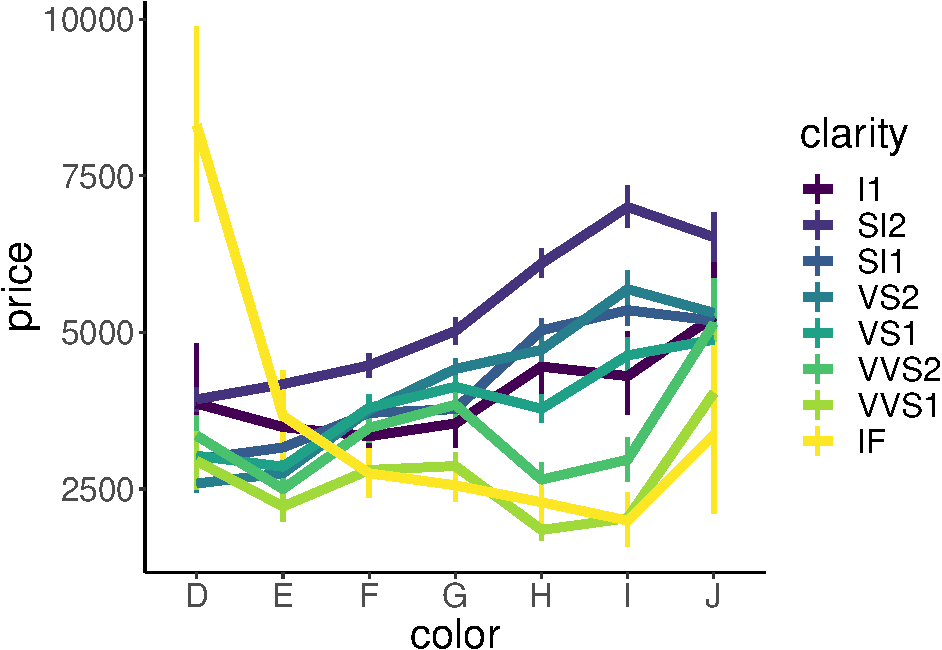
\includegraphics{02-visualization1_files/figure-latex/visualization1-49-1.pdf}

\begin{Shaded}
\begin{Highlighting}[]
\KeywordTok{include_graphics}\NormalTok{(}\StringTok{"figures/practice_plot3.png"}\NormalTok{)}
\end{Highlighting}
\end{Shaded}

\begin{figure}

{\centering 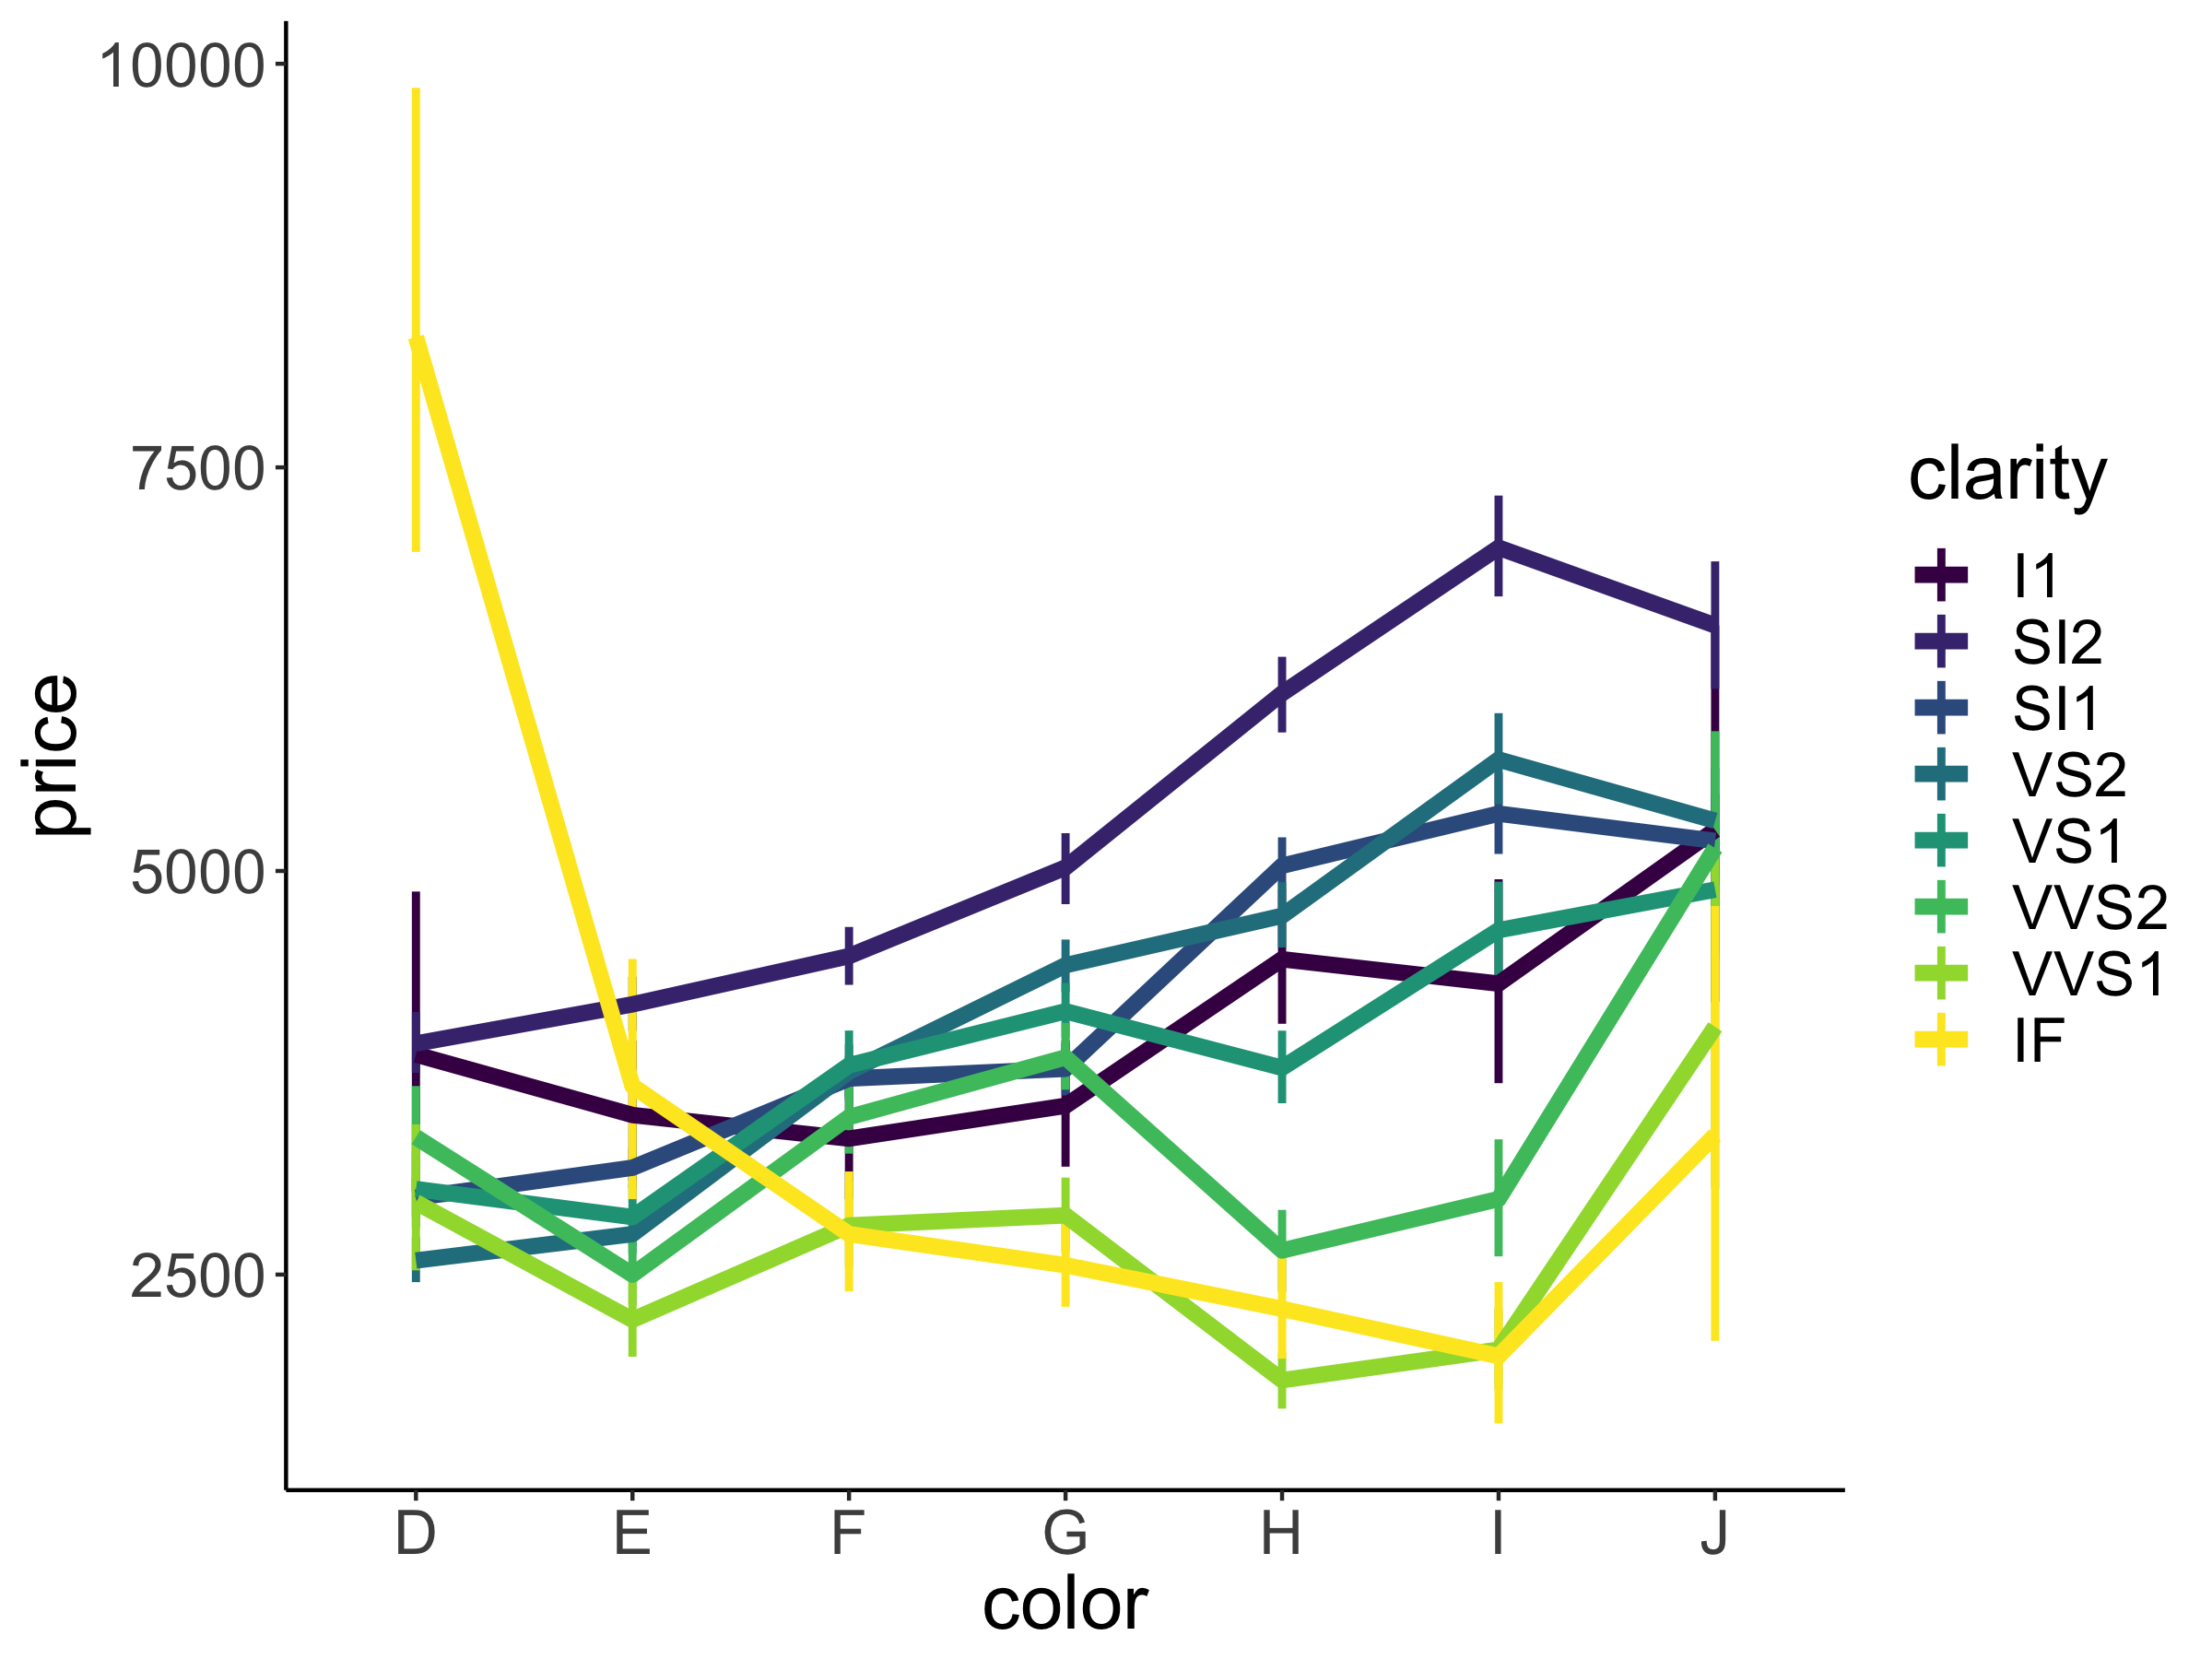
\includegraphics[width=0.9\linewidth]{figures/practice_plot3} 

}

\caption{Practice plot 3.}\label{fig:visualization1-50}
\end{figure}

\hypertarget{making-facets}{%
\subsection{Making facets}\label{making-facets}}

Having too much information in a single plot can be overwhelming. The previous plot is already pretty busy. Facets are a nice way of spliting up plots and showing information in separate panels.

Let's take a look at how wide these diamonds tend to be. The width in mm is given in the \texttt{y} column of the diamonds data frame. We'll make a histogram first. To make a histogram, the only aesthetic we needed to specify is \texttt{x}.

\begin{Shaded}
\begin{Highlighting}[]
\KeywordTok{ggplot}\NormalTok{(}\DataTypeTok{data =}\NormalTok{ df.diamonds,}
       \DataTypeTok{mapping =} \KeywordTok{aes}\NormalTok{(}\DataTypeTok{x =}\NormalTok{ y)) }\OperatorTok{+}
\StringTok{  }\KeywordTok{geom_histogram}\NormalTok{()}
\end{Highlighting}
\end{Shaded}

\begin{verbatim}
## `stat_bin()` using `bins = 30`. Pick better value with `binwidth`.
\end{verbatim}

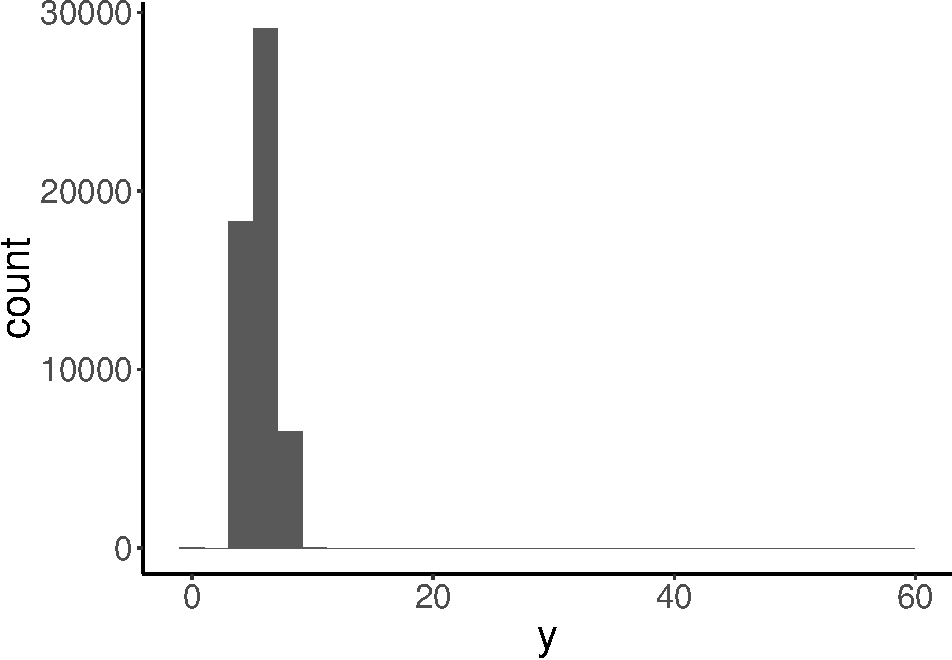
\includegraphics{02-visualization1_files/figure-latex/visualization1-51-1.pdf}

That looks bad! Let's pick a different value for the width of the bins in the histogram.

\begin{Shaded}
\begin{Highlighting}[]
\KeywordTok{ggplot}\NormalTok{(}\DataTypeTok{data =}\NormalTok{ df.diamonds, }\DataTypeTok{mapping =} \KeywordTok{aes}\NormalTok{(}\DataTypeTok{x =}\NormalTok{ y)) }\OperatorTok{+}
\StringTok{  }\KeywordTok{geom_histogram}\NormalTok{(}\DataTypeTok{binwidth =} \FloatTok{0.1}\NormalTok{)}
\end{Highlighting}
\end{Shaded}

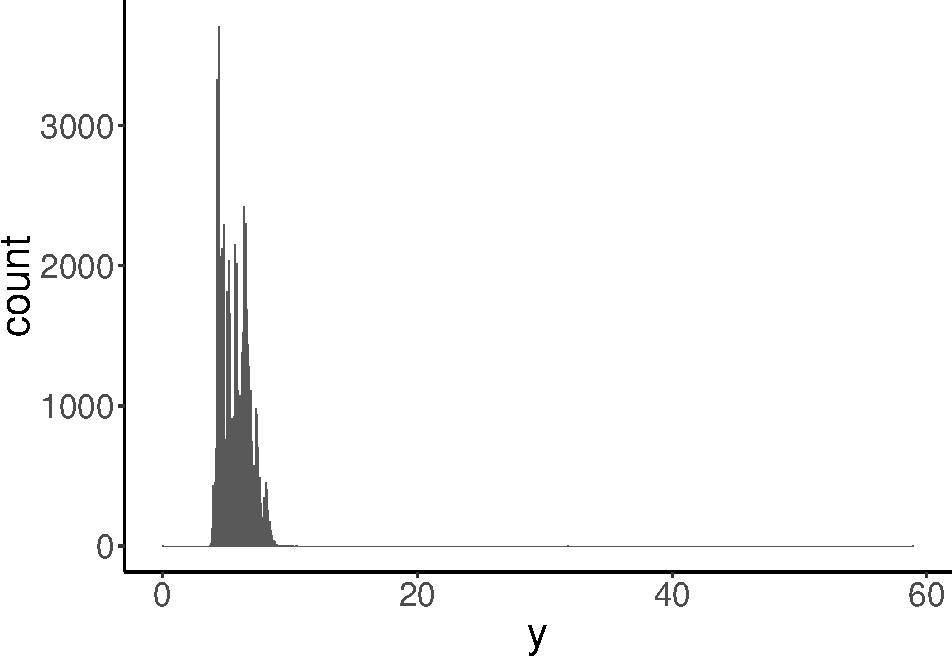
\includegraphics{02-visualization1_files/figure-latex/visualization1-52-1.pdf}

Still bad. There seems to be an outlier diamond that happens to be almost 60 mm wide, while most of the rest is much narrower. One option would be to remove the outlier from the data before plotting it. But generally, we don't want to make new data frames. Instead, let's just limit what data we want to show in the plot.

\begin{Shaded}
\begin{Highlighting}[]
\KeywordTok{ggplot}\NormalTok{(}\DataTypeTok{data =}\NormalTok{ df.diamonds, }\DataTypeTok{mapping =} \KeywordTok{aes}\NormalTok{(}\DataTypeTok{x =}\NormalTok{ y)) }\OperatorTok{+}
\StringTok{  }\KeywordTok{geom_histogram}\NormalTok{(}\DataTypeTok{binwidth =} \FloatTok{0.1}\NormalTok{) }\OperatorTok{+}
\StringTok{  }\KeywordTok{coord_cartesian}\NormalTok{(}\DataTypeTok{xlim =} \KeywordTok{c}\NormalTok{(}\DecValTok{3}\NormalTok{, }\DecValTok{10}\NormalTok{))}
\end{Highlighting}
\end{Shaded}

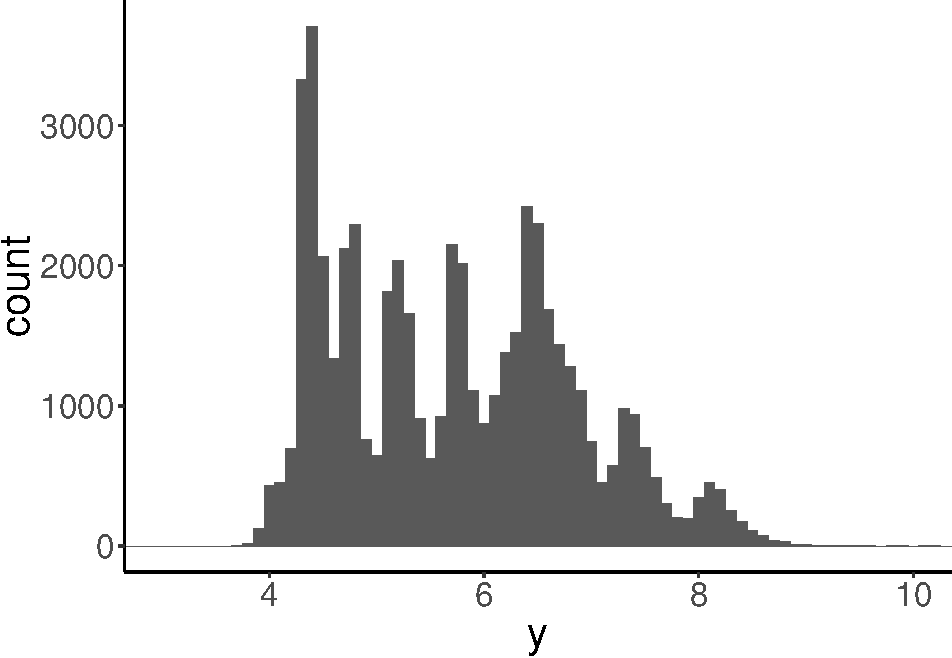
\includegraphics{02-visualization1_files/figure-latex/visualization1-53-1.pdf}

I've used the \texttt{coord\_cartesian()} function to restrict the range of data to show by passing a minimum and maximum to the \texttt{xlim} argument. This looks better now.

Instead of histograms, we can also plot a density fitted to the distribution.

\begin{Shaded}
\begin{Highlighting}[]
\KeywordTok{ggplot}\NormalTok{(}\DataTypeTok{data =}\NormalTok{ df.diamonds, }\DataTypeTok{mapping =} \KeywordTok{aes}\NormalTok{(}\DataTypeTok{x =}\NormalTok{ y)) }\OperatorTok{+}
\StringTok{  }\KeywordTok{geom_density}\NormalTok{() }\OperatorTok{+}
\StringTok{  }\KeywordTok{coord_cartesian}\NormalTok{(}\DataTypeTok{xlim =} \KeywordTok{c}\NormalTok{(}\DecValTok{3}\NormalTok{, }\DecValTok{10}\NormalTok{))}
\end{Highlighting}
\end{Shaded}

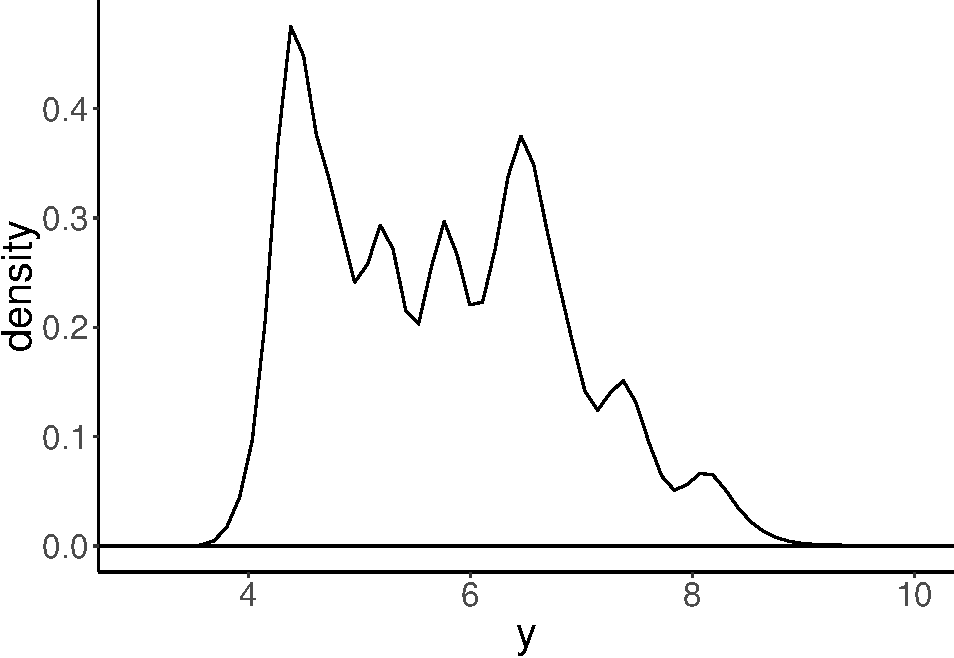
\includegraphics{02-visualization1_files/figure-latex/visualization1-54-1.pdf}

Looks pretty similar to our histogram above! Just like we can play around with the binwidth of the histogram, we can change the smoothing bandwidth of the kernel that is used to create the histogram. Here is a histogram with a much wider bandwidth:

\begin{Shaded}
\begin{Highlighting}[]
\KeywordTok{ggplot}\NormalTok{(}\DataTypeTok{data =}\NormalTok{ df.diamonds, }\DataTypeTok{mapping =} \KeywordTok{aes}\NormalTok{(}\DataTypeTok{x =}\NormalTok{ y)) }\OperatorTok{+}
\StringTok{  }\KeywordTok{geom_density}\NormalTok{(}\DataTypeTok{bw =} \FloatTok{0.5}\NormalTok{) }\OperatorTok{+}
\StringTok{  }\KeywordTok{coord_cartesian}\NormalTok{(}\DataTypeTok{xlim =} \KeywordTok{c}\NormalTok{(}\DecValTok{3}\NormalTok{, }\DecValTok{10}\NormalTok{))}
\end{Highlighting}
\end{Shaded}

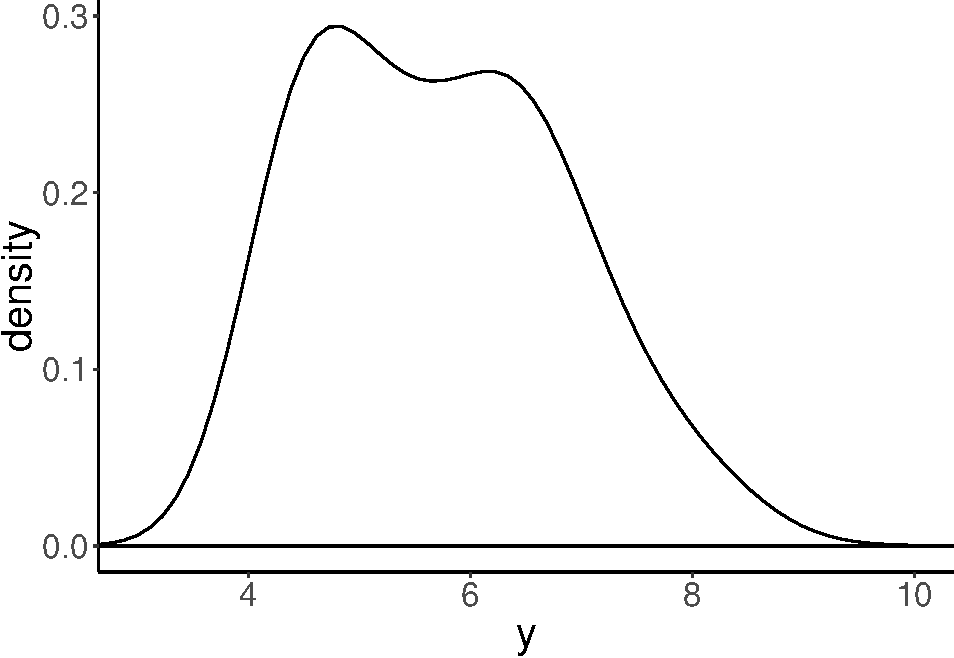
\includegraphics{02-visualization1_files/figure-latex/visualization1-55-1.pdf}

We'll learn more about how these densities are determined later in class.

I promised that this section was about making facets, right? We're getting there! Let's first take a look at how wide diamonds of different \texttt{color} are. We can use grouping to make this happen.

\begin{Shaded}
\begin{Highlighting}[]
\KeywordTok{ggplot}\NormalTok{(}\DataTypeTok{data =}\NormalTok{ df.diamonds,}
       \DataTypeTok{mapping =} \KeywordTok{aes}\NormalTok{(}\DataTypeTok{x =}\NormalTok{ y,}
                     \DataTypeTok{group =}\NormalTok{ color,}
                     \DataTypeTok{fill =}\NormalTok{ color)) }\OperatorTok{+}
\StringTok{  }\KeywordTok{geom_density}\NormalTok{(}\DataTypeTok{bw =} \FloatTok{0.2}\NormalTok{, }\DataTypeTok{alpha =} \FloatTok{0.2}\NormalTok{) }\OperatorTok{+}
\StringTok{  }\KeywordTok{coord_cartesian}\NormalTok{(}\DataTypeTok{xlim =} \KeywordTok{c}\NormalTok{(}\DecValTok{3}\NormalTok{, }\DecValTok{10}\NormalTok{))}
\end{Highlighting}
\end{Shaded}

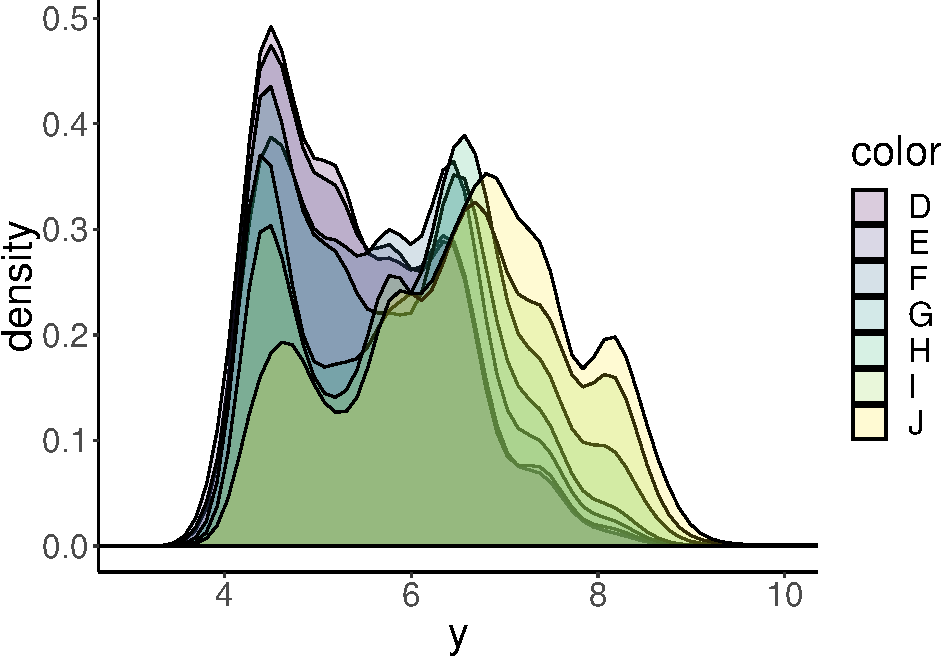
\includegraphics{02-visualization1_files/figure-latex/visualization1-56-1.pdf}

OK! That's a little tricky to tell apart. Notice that I've specified the \texttt{alpha} argument in the \texttt{geom\_density()} function so that the densities in the front don't completely hide the densities in the back. But this plot still looks too busy. Instead of grouping, let's put the densities for the different colors, in separate panels. That's what facetting allows you to do.

\begin{Shaded}
\begin{Highlighting}[]
\KeywordTok{ggplot}\NormalTok{(}\DataTypeTok{data =}\NormalTok{ df.diamonds,}
       \DataTypeTok{mapping =} \KeywordTok{aes}\NormalTok{(}\DataTypeTok{x =}\NormalTok{ y, }\DataTypeTok{fill =}\NormalTok{ color)) }\OperatorTok{+}
\StringTok{  }\KeywordTok{geom_density}\NormalTok{(}\DataTypeTok{bw =} \FloatTok{0.2}\NormalTok{) }\OperatorTok{+}
\StringTok{  }\KeywordTok{facet_grid}\NormalTok{(}\DataTypeTok{cols =} \KeywordTok{vars}\NormalTok{(color)) }\OperatorTok{+}
\StringTok{  }\KeywordTok{coord_cartesian}\NormalTok{(}\DataTypeTok{xlim =} \KeywordTok{c}\NormalTok{(}\DecValTok{3}\NormalTok{, }\DecValTok{10}\NormalTok{))}
\end{Highlighting}
\end{Shaded}

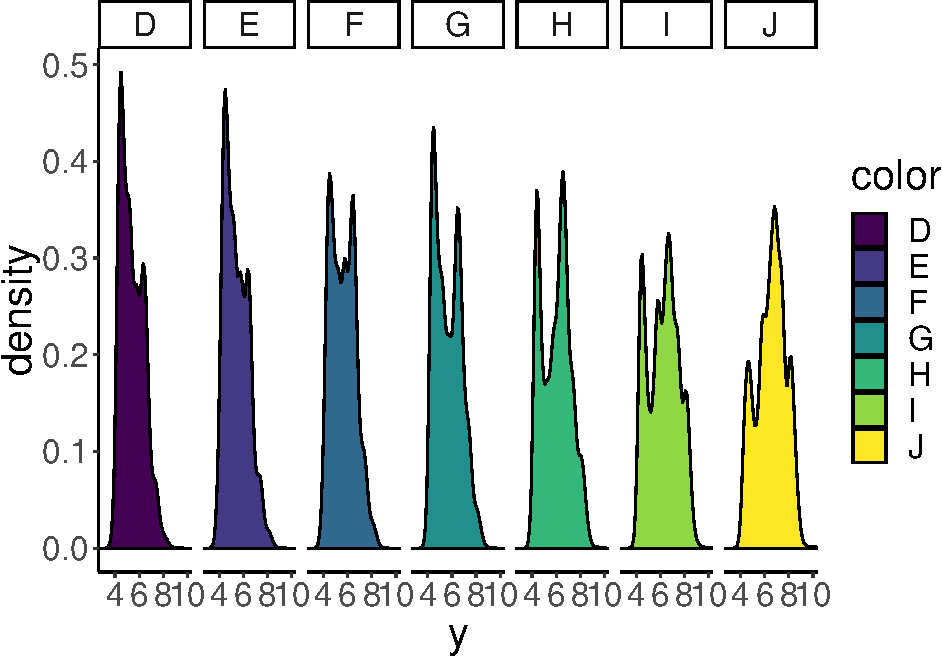
\includegraphics{02-visualization1_files/figure-latex/visualization1-57-1.pdf}

Now we have the densities next to each other in separate panels. I've removed the \texttt{alpha} argument since the densities aren't overlapping anymore. To make the different panels, I used the \texttt{facet\_grid()} function and specified that I want separate columns for the different colors (\texttt{cols\ =\ vars(color)}). What's the deal with \texttt{vars()}? Why couldn't we just write \texttt{facet\_grid(cols\ =\ color)} instead? The short answer is: that's what the function wants. The long answer is: long. (We'll learn more about this later in the course.)

To show the facets in different rows instead of columns we simply replace \texttt{cols\ =\ vars(color)} with \texttt{rows\ =\ vars(color)}.

\begin{Shaded}
\begin{Highlighting}[]
\KeywordTok{ggplot}\NormalTok{(}\DataTypeTok{data =}\NormalTok{ df.diamonds, }\DataTypeTok{mapping =} \KeywordTok{aes}\NormalTok{(}\DataTypeTok{x =}\NormalTok{ y, }\DataTypeTok{fill =}\NormalTok{ color)) }\OperatorTok{+}
\StringTok{  }\KeywordTok{geom_density}\NormalTok{(}\DataTypeTok{bw =} \FloatTok{0.2}\NormalTok{) }\OperatorTok{+}
\StringTok{  }\KeywordTok{facet_grid}\NormalTok{(}\DataTypeTok{rows =} \KeywordTok{vars}\NormalTok{(color)) }\OperatorTok{+}
\StringTok{  }\KeywordTok{coord_cartesian}\NormalTok{(}\DataTypeTok{xlim =} \KeywordTok{c}\NormalTok{(}\DecValTok{3}\NormalTok{, }\DecValTok{10}\NormalTok{))}
\end{Highlighting}
\end{Shaded}

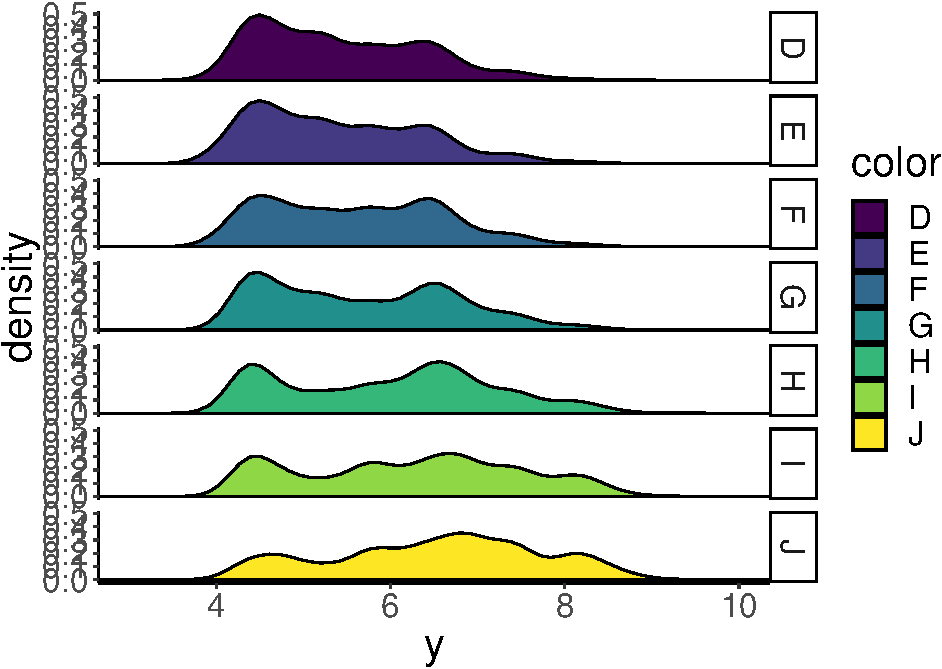
\includegraphics{02-visualization1_files/figure-latex/visualization1-58-1.pdf}

Several aspects about this plot should be improved:

\begin{itemize}
\tightlist
\item
  the y-axis text is overlapping
\item
  having both a legend and separate facet labels is redundant
\item
  having separate fills is not really necessary here
\end{itemize}

So, what does this plot actually show us? Well, J-colored diamonds tend to be wider than D-colored diamonds. Fascinating!

Of course, we could go completely overboard with facets and groups. So let's do it! Let's look at how the average \texttt{price} (somewhat more interesting) varies as a function of \texttt{color}, \texttt{cut}, and \texttt{clarity}. We'll put color on the x-axis, and make separate rows for \texttt{cut} and columns for \texttt{clarity}.

\begin{Shaded}
\begin{Highlighting}[]
\KeywordTok{ggplot}\NormalTok{(}\DataTypeTok{data =}\NormalTok{ df.diamonds,}
       \DataTypeTok{mapping =} \KeywordTok{aes}\NormalTok{(}\DataTypeTok{y =}\NormalTok{ price,}
                     \DataTypeTok{x =}\NormalTok{ color,}
                     \DataTypeTok{fill =}\NormalTok{ color)) }\OperatorTok{+}
\StringTok{  }\KeywordTok{stat_summary}\NormalTok{(}\DataTypeTok{fun.y =} \StringTok{"mean"}\NormalTok{,}
               \DataTypeTok{geom =} \StringTok{"bar"}\NormalTok{,}
               \DataTypeTok{color =} \StringTok{"black"}\NormalTok{) }\OperatorTok{+}
\StringTok{  }\KeywordTok{stat_summary}\NormalTok{(}\DataTypeTok{fun.data =} \StringTok{"mean_cl_boot"}\NormalTok{,}
               \DataTypeTok{geom =} \StringTok{"linerange"}\NormalTok{) }\OperatorTok{+}
\StringTok{  }\KeywordTok{facet_grid}\NormalTok{(}\DataTypeTok{rows =} \KeywordTok{vars}\NormalTok{(cut),}
             \DataTypeTok{cols =} \KeywordTok{vars}\NormalTok{(clarity))}
\end{Highlighting}
\end{Shaded}

\begin{verbatim}
## Warning: Removed 5 rows containing missing values (geom_linerange).
\end{verbatim}

\begin{figure}
\centering
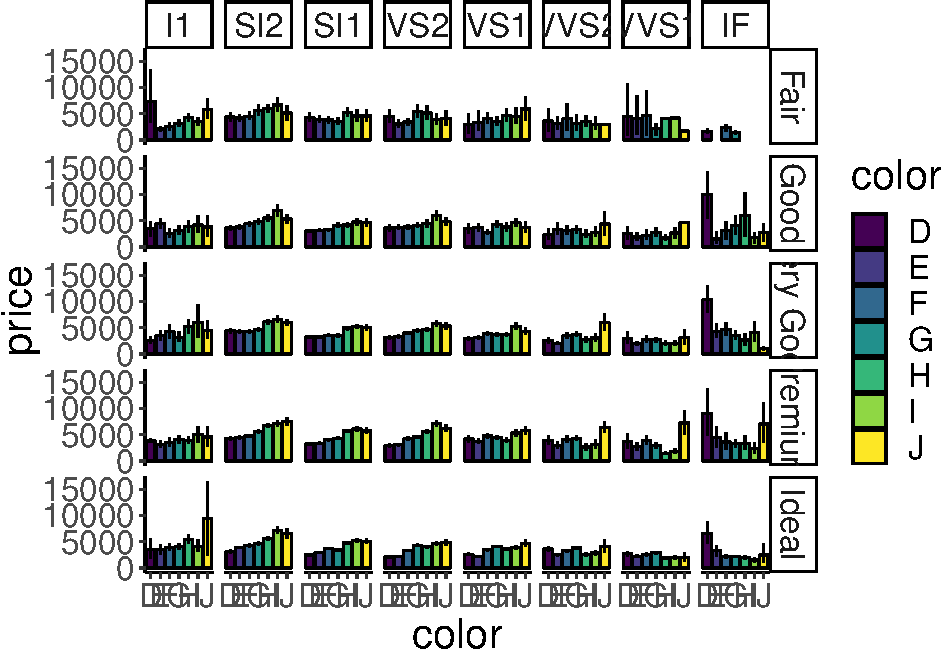
\includegraphics{02-visualization1_files/figure-latex/visualization1-59-1.pdf}
\caption{\label{fig:visualization1-59}A figure that is stretching it in terms of information.}
\end{figure}

Figure \ref{fig:visualization-57} is stretching it in terms of how much information it presents. But it gives you a sense for how to combine the differnet bits and pieces we've learned so far.

\hypertarget{practice-plot-4}{%
\subsubsection{Practice plot 4}\label{practice-plot-4}}

Recreate the plot shown in Figure \ref{fig:visualization-59}.

\begin{Shaded}
\begin{Highlighting}[]
\CommentTok{# make practice plot 4 here}
\KeywordTok{ggplot}\NormalTok{(diamonds, }\KeywordTok{aes}\NormalTok{(}\DataTypeTok{x =}\NormalTok{ color, }\DataTypeTok{y =}\NormalTok{ price, }\DataTypeTok{fill =}\NormalTok{ cut))}\OperatorTok{+}
\StringTok{  }\KeywordTok{stat_summary}\NormalTok{(}\DataTypeTok{fun.y =} \StringTok{"mean"}\NormalTok{,}
               \DataTypeTok{geom =} \StringTok{"bar"}\NormalTok{,}
               \DataTypeTok{position =} \KeywordTok{position_dodge}\NormalTok{(}\DataTypeTok{width =} \FloatTok{0.9}\NormalTok{),}
               \DataTypeTok{color =} \StringTok{"black"}\NormalTok{)}\OperatorTok{+}
\StringTok{  }\KeywordTok{stat_summary}\NormalTok{(}\DataTypeTok{fun.data =} \StringTok{"mean_cl_boot"}\NormalTok{,}
               \DataTypeTok{geom =} \StringTok{"linerange"}\NormalTok{,}
               \DataTypeTok{position =} \KeywordTok{position_dodge}\NormalTok{(}\DataTypeTok{width =} \FloatTok{0.9}\NormalTok{),}
               \DataTypeTok{color =} \StringTok{"black"}\NormalTok{)}\OperatorTok{+}
\StringTok{  }\KeywordTok{facet_grid}\NormalTok{(}\DataTypeTok{rows =} \KeywordTok{vars}\NormalTok{(clarity)) }\OperatorTok{+}
\StringTok{  }\KeywordTok{theme}\NormalTok{(}\DataTypeTok{axis.text.y =} \KeywordTok{element_text}\NormalTok{(}\DataTypeTok{size =} \DecValTok{10}\NormalTok{))}
\end{Highlighting}
\end{Shaded}

\begin{verbatim}
## Warning: Removed 5 rows containing missing values (geom_linerange).
\end{verbatim}

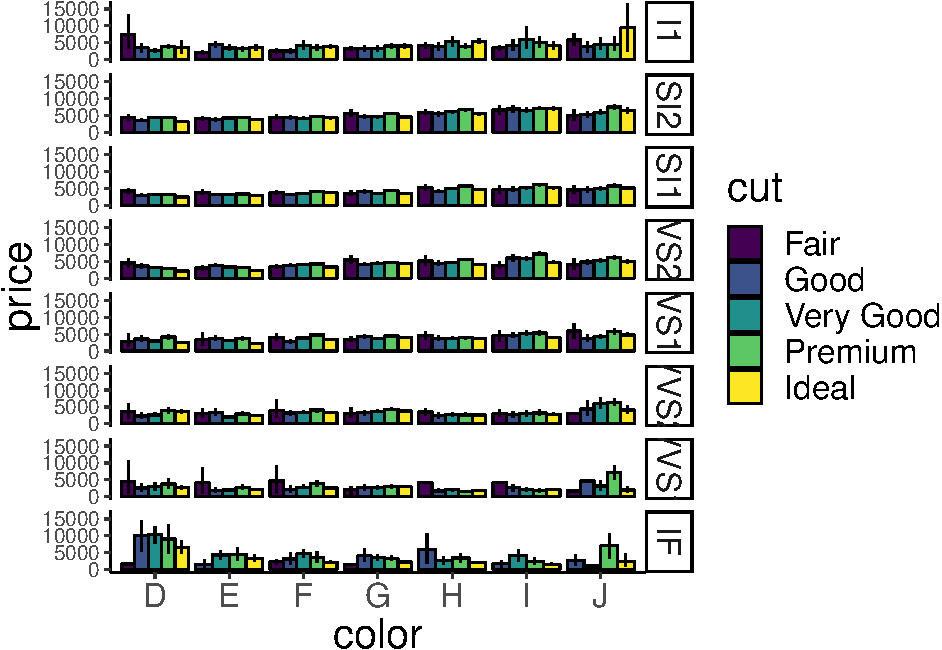
\includegraphics{02-visualization1_files/figure-latex/visualization1-60-1.pdf}

\begin{Shaded}
\begin{Highlighting}[]
\KeywordTok{include_graphics}\NormalTok{(}\StringTok{"figures/practice_plot4.png"}\NormalTok{)}
\end{Highlighting}
\end{Shaded}

\begin{figure}

{\centering 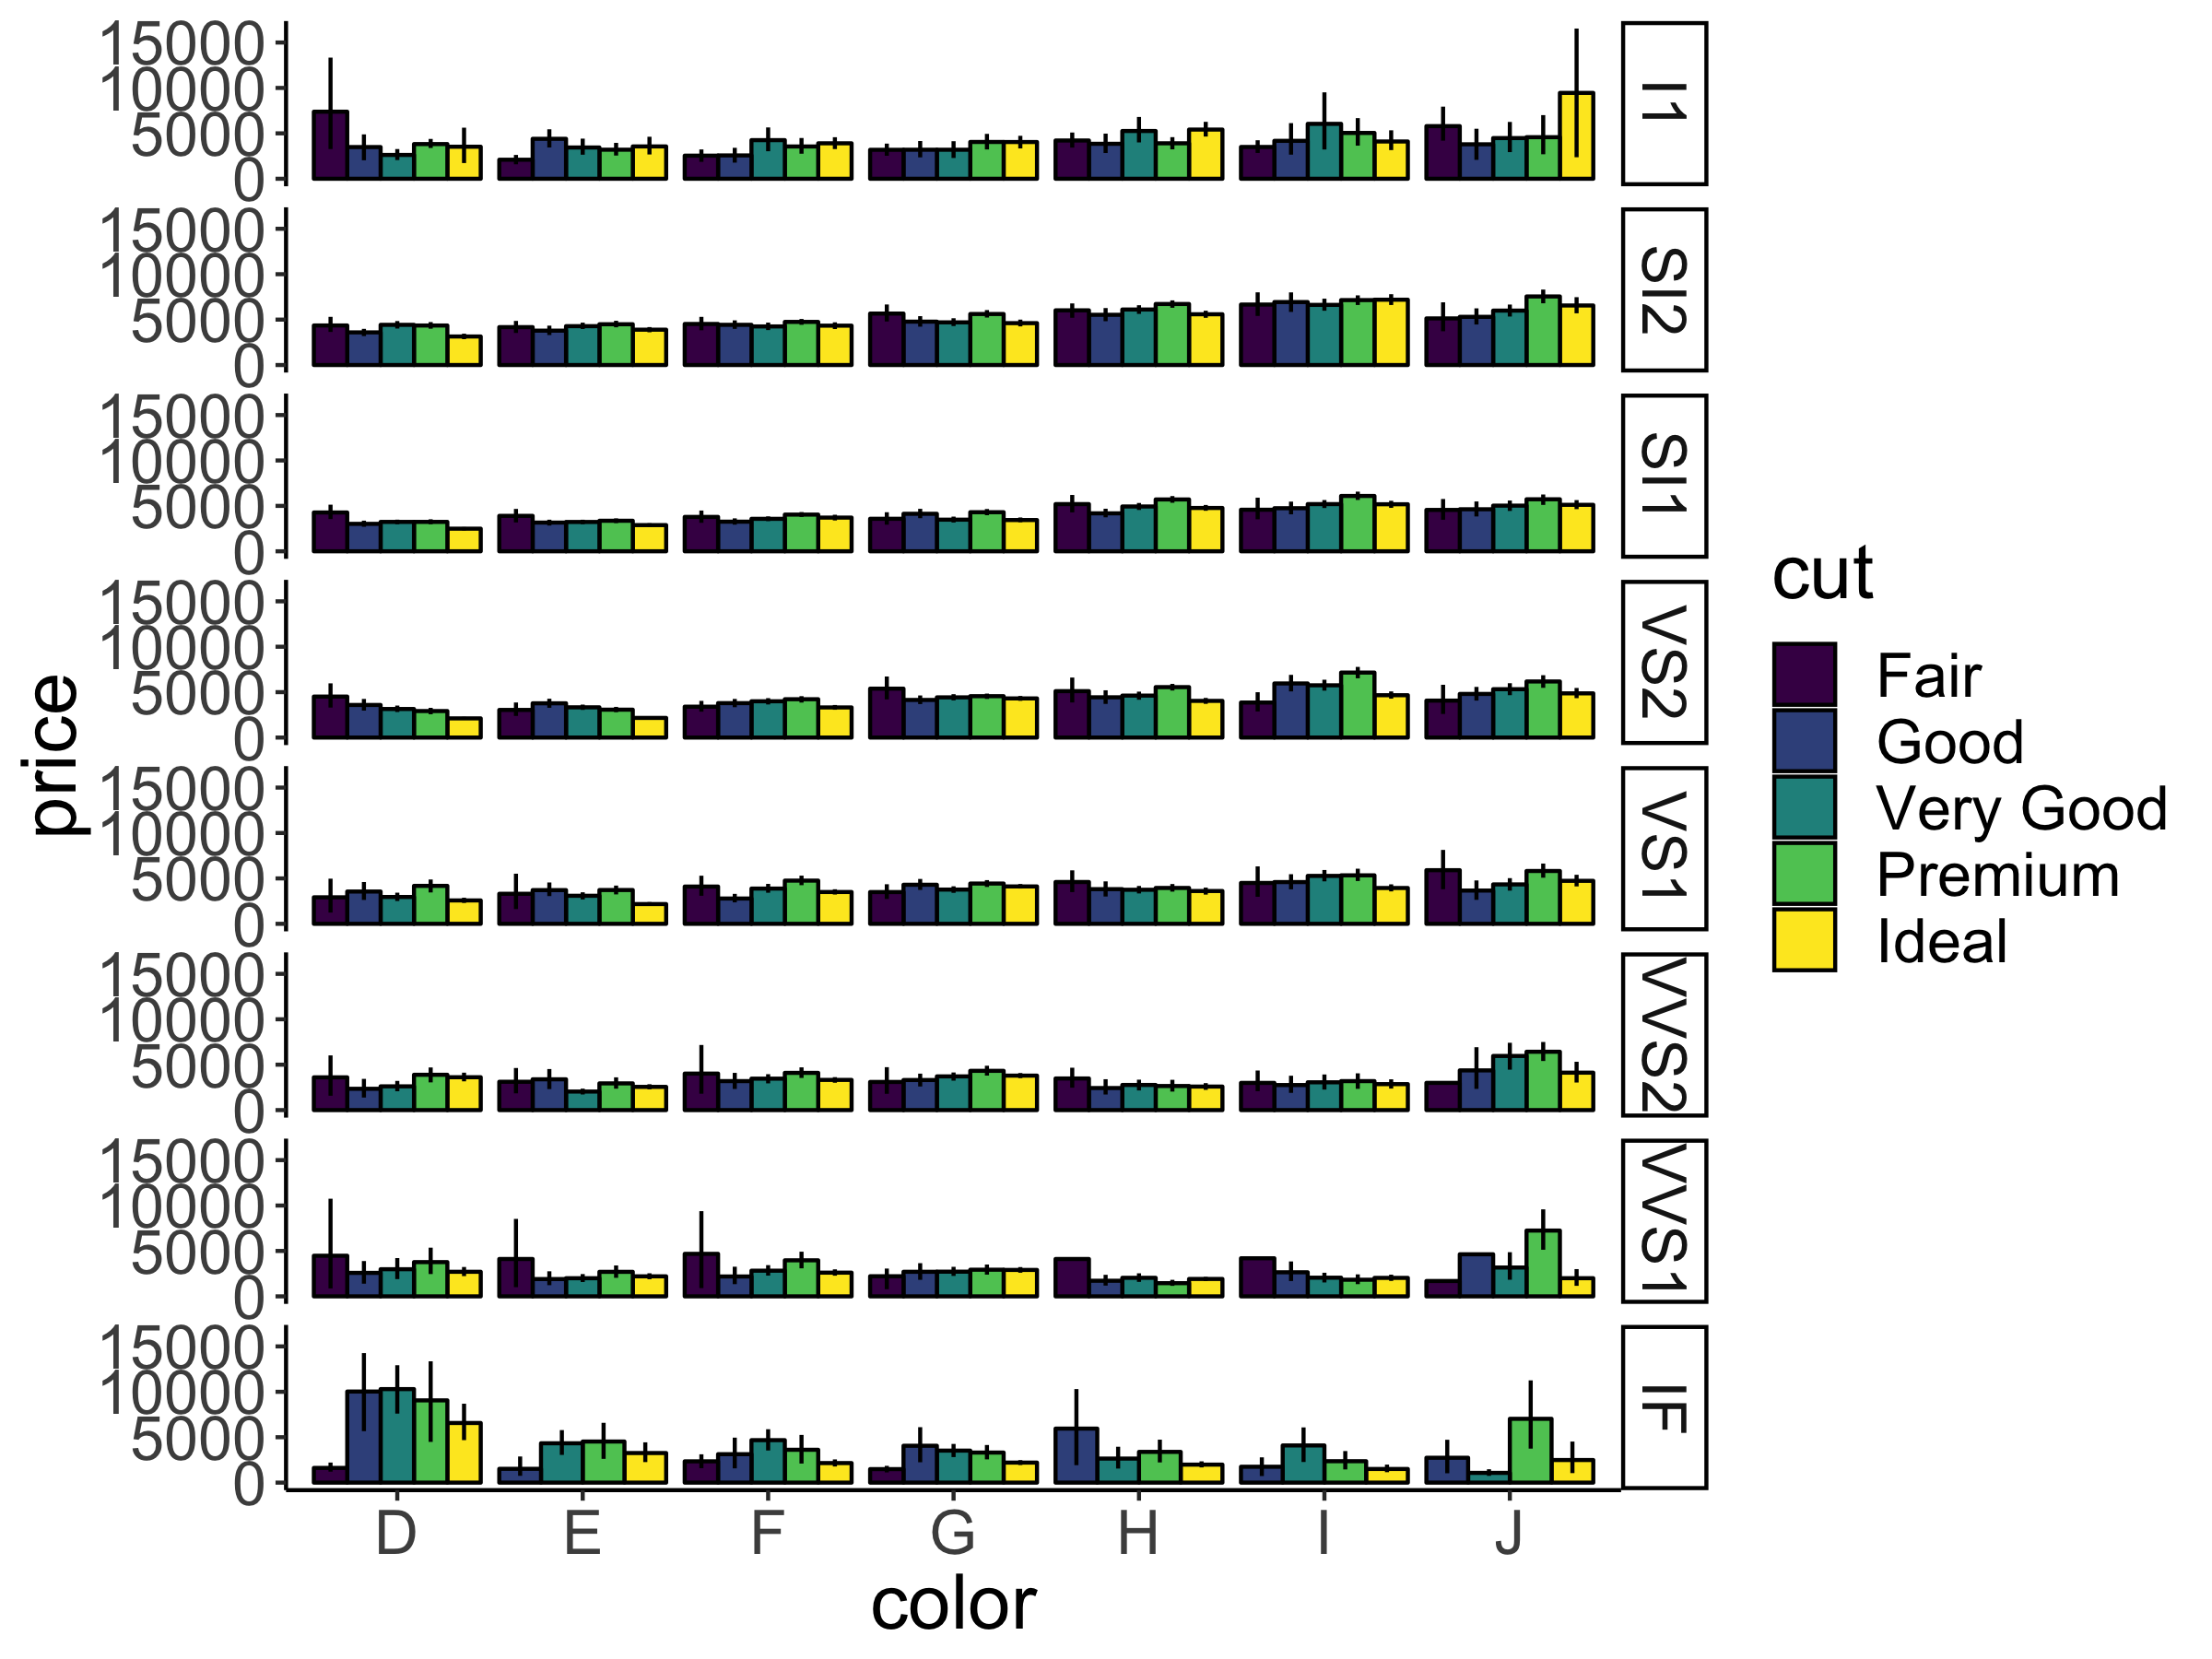
\includegraphics[width=0.9\linewidth]{figures/practice_plot4} 

}

\caption{Practice plot 4.}\label{fig:visualization1-61}
\end{figure}

\hypertarget{global-local-and-setting-aes}{%
\subsection{\texorpdfstring{Global, local, and setting \texttt{aes()}}{Global, local, and setting aes()}}\label{global-local-and-setting-aes}}

\texttt{ggplot2} allows you to specify the plot aesthetics in different ways.

\begin{Shaded}
\begin{Highlighting}[]
\KeywordTok{ggplot}\NormalTok{(}\DataTypeTok{data =}\NormalTok{ df.diamonds,}
       \DataTypeTok{mapping =} \KeywordTok{aes}\NormalTok{(}\DataTypeTok{x =}\NormalTok{ carat,}
                     \DataTypeTok{y =}\NormalTok{ price,}
                     \DataTypeTok{color =}\NormalTok{ color)) }\OperatorTok{+}
\StringTok{  }\KeywordTok{geom_point}\NormalTok{() }\OperatorTok{+}
\StringTok{  }\KeywordTok{geom_smooth}\NormalTok{(}\DataTypeTok{method =} \StringTok{"lm"}\NormalTok{, }\DataTypeTok{se =}\NormalTok{ F)}
\end{Highlighting}
\end{Shaded}

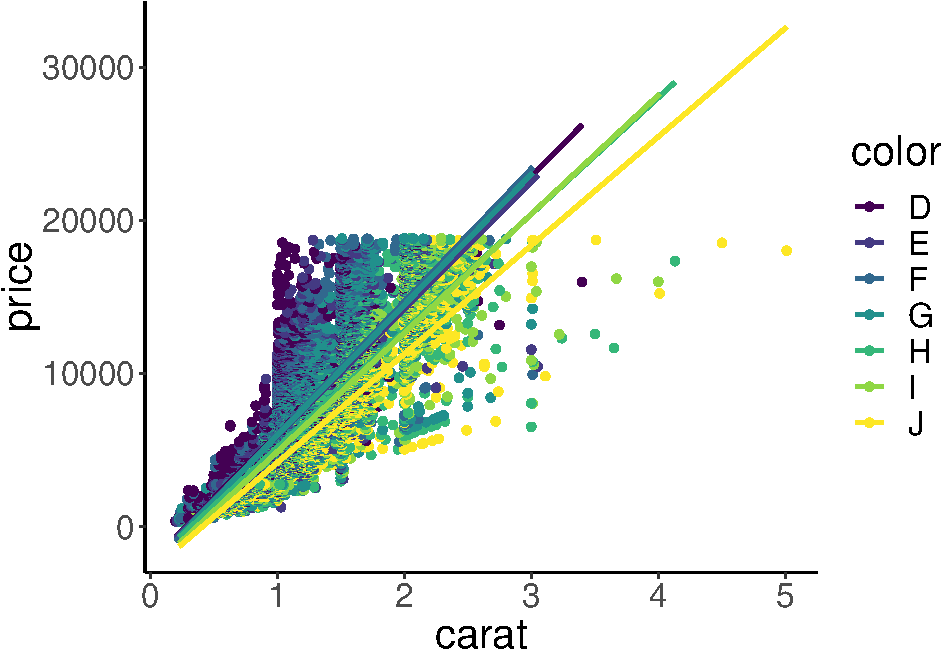
\includegraphics{02-visualization1_files/figure-latex/visualization1-62-1.pdf}

Here, I've drawn a scatter plot of the relationship between \texttt{carat} and \texttt{price}, and I have added the best-fitting regression lines via the \texttt{geom\_smooth(method\ =\ "lm")} call. (We will learn more about what these regression lines mean later in class.)

Because I have defined all the aesthetics at the top level (i.e.~directly within the \texttt{ggplot()} function), the aesthetics apply to all the functions afterwards. Aesthetics defined in the \texttt{ggplot()} call are \textbf{global}. In this case, the \texttt{geom\_point()} and the \texttt{geom\_smooth()} functions. The \texttt{geom\_smooth()} function produces separate best-fit regression lines for each different color.

But what if we only wanted to show one regression line instead that applies to all the data? Here is one way of doing so:

\begin{Shaded}
\begin{Highlighting}[]
\KeywordTok{ggplot}\NormalTok{(}\DataTypeTok{data =}\NormalTok{ df.diamonds, }\DataTypeTok{mapping =} \KeywordTok{aes}\NormalTok{(}\DataTypeTok{x =}\NormalTok{ carat, }\DataTypeTok{y =}\NormalTok{ price)) }\OperatorTok{+}
\StringTok{  }\KeywordTok{geom_point}\NormalTok{(}\DataTypeTok{mapping =} \KeywordTok{aes}\NormalTok{(}\DataTypeTok{color =}\NormalTok{ color)) }\OperatorTok{+}
\StringTok{  }\KeywordTok{geom_smooth}\NormalTok{(}\DataTypeTok{method =} \StringTok{"lm"}\NormalTok{)}
\end{Highlighting}
\end{Shaded}

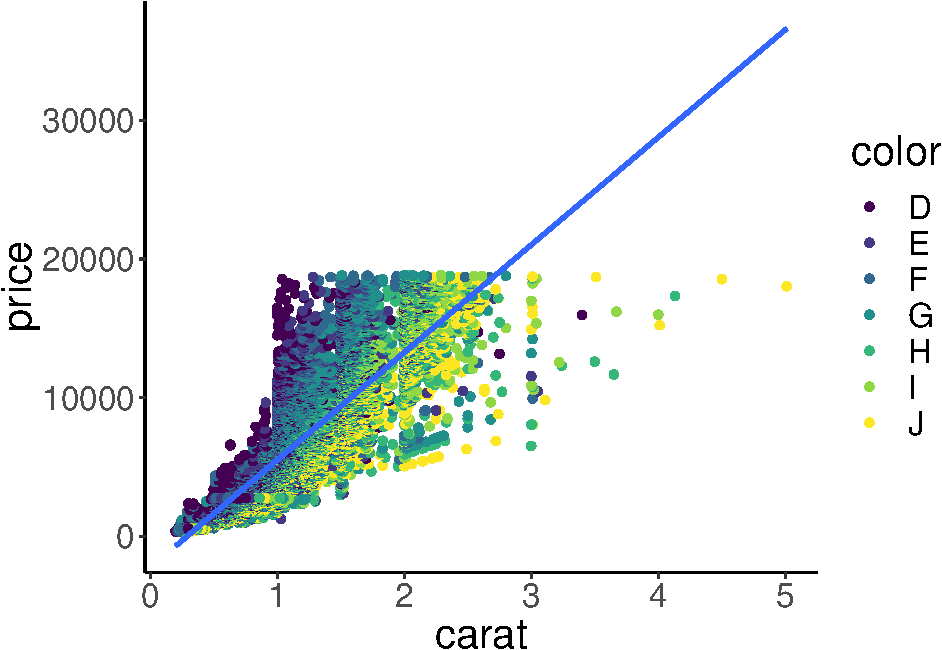
\includegraphics{02-visualization1_files/figure-latex/visualization1-63-1.pdf}

Here, I've moved the color aesthetic into the \texttt{geom\_point()} function call. Now, the \texttt{x} and \texttt{y} aesthetics still apply to both the \texttt{geom\_point()} and the \texttt{geom\_smooth()} function call (they are \textbf{global}), but the \texttt{color} aesthetic applies only to \texttt{geom\_point()} (it is \textbf{local}). Alternatively, we can simply overwrite global aesthetics within local function calls.

\begin{Shaded}
\begin{Highlighting}[]
\KeywordTok{ggplot}\NormalTok{(}\DataTypeTok{data =}\NormalTok{ df.diamonds, }\KeywordTok{aes}\NormalTok{(}\DataTypeTok{x =}\NormalTok{ carat, }\DataTypeTok{y =}\NormalTok{ price, }\DataTypeTok{color =}\NormalTok{ color)) }\OperatorTok{+}
\StringTok{  }\KeywordTok{geom_point}\NormalTok{() }\OperatorTok{+}
\StringTok{  }\KeywordTok{geom_smooth}\NormalTok{(}\DataTypeTok{method =} \StringTok{"lm"}\NormalTok{, }\DataTypeTok{color =} \StringTok{"black"}\NormalTok{)}
\end{Highlighting}
\end{Shaded}

\includegraphics{02-visualization1_files/figure-latex/visualization1-64-1.pdf}

Here, I've set \texttt{color\ =\ \textquotesingle{}black\textquotesingle{}} within the \texttt{geom\_smooth()} function, and now only one overall regression line is displayed since the global color aesthetic was overwritten in the local function call.

\hypertarget{additional-resources}{%
\section{Additional resources}\label{additional-resources}}

\hypertarget{cheatsheets}{%
\subsection{Cheatsheets}\label{cheatsheets}}

\begin{itemize}
\tightlist
\item
  \href{figures/rstudio-ide.pdf}{RStudio IDE} --\textgreater{} information about RStudio
\item
  \href{figures/rmarkdown.pdf}{RMarkdown} --\textgreater{} information about writing in RMarkdown
\item
  \href{figures/rmarkdown-reference.pdf}{RMarkdown reference} --\textgreater{} RMarkdown reference sheet
\item
  \href{figures/visualization-principles.pdf}{Data visualization} --\textgreater{} general principles of effective graphic design
\item
  \href{figures/data-visualization.pdf}{ggplot2} --\textgreater{} specific information about ggplot
\end{itemize}

\hypertarget{data-camp-courses}{%
\subsection{Data camp courses}\label{data-camp-courses}}

\begin{itemize}
\tightlist
\item
  \href{https://www.datacamp.com/courses/free-introduction-to-r}{Introduction to R}
\item
  \href{https://www.datacamp.com/courses/working-with-the-rstudio-ide-part-1}{RStudio IDE 1}
\item
  \href{https://www.datacamp.com/courses/working-with-the-rstudio-ide-part-2}{RStudio IDE 2}
\item
  \href{https://www.datacamp.com/courses/communicating-with-data-in-the-tidyverse}{Communicating with data}
\item
  \href{https://www.datacamp.com/courses/data-visualization-with-ggplot2-1}{ggplot2 course 1}
\item
  \href{https://www.datacamp.com/courses/data-visualization-with-ggplot2-2}{ggplot2 course 2}
\end{itemize}

\hypertarget{books-and-chapters}{%
\subsection{Books and chapters}\label{books-and-chapters}}

\begin{itemize}
\tightlist
\item
  \href{http://www.cookbook-r.com/Graphs/}{R graphics cookbook} --\textgreater{} quick intro to the the most common graphs
\item
  \href{http://r4ds.had.co.nz/}{R for Data Science book}

  \begin{itemize}
  \tightlist
  \item
    \href{http://r4ds.had.co.nz/data-visualisation.html}{Data visualization}
  \item
    \href{http://r4ds.had.co.nz/graphics-for-communication.html}{Graphics for communication}
  \end{itemize}
\item
  \href{http://socviz.co/}{Data Visualization -- A practical introduction (by Kieran Healy)}

  \begin{itemize}
  \tightlist
  \item
    \href{http://socviz.co/lookatdata.html\#lookatdata}{Look at data}
  \item
    \href{http://socviz.co/makeplot.html\#makeplot}{Make a plot}
  \item
    \href{http://socviz.co/groupfacettx.html\#groupfacettx}{Show the right numbers}
  \end{itemize}
\item
  \href{https://serialmentor.com/dataviz/}{Fundamentals of Data Visualization} --\textgreater{} very nice resource that goes beyond basic functionality of \texttt{ggplot} and focuses on how to make good figures (e.g.~how to choose colors, axes, \ldots)
\end{itemize}

\hypertarget{misc}{%
\subsection{Misc}\label{misc}}

\begin{itemize}
\tightlist
\item
  \href{http://www.ggplot2-exts.org/gallery/}{ggplot2 extensions} --\textgreater{} gallery of ggplot2 extension packages
\item
  \href{https://github.com/dreamRs/esquisse}{ggplot2 gui} --\textgreater{} ggplot2 extension package
\item
  \href{http://r-statistics.co/Top50-Ggplot2-Visualizations-MasterList-R-Code.html}{ggplot2 visualizations with code} --\textgreater{} gallery of plots with code
\item
  \href{https://rmarkdown.rstudio.com/lesson-1.html}{R Markdown in RStudio introduction}
\item
  \href{http://www.stat.cmu.edu/~cshalizi/rmarkdown/}{R Markdown for class reports}
\item
  \href{https://kbroman.org/knitr_knutshell/}{knitr in a nutshell}
\item
  \href{https://github.com/r-lib/styler}{styler} --\textgreater{} RStudio add-in that re-formats code
\end{itemize}

\hypertarget{visualization-2}{%
\chapter{Visualization 2}\label{visualization-2}}

In this lecture, we will lift our \texttt{ggplot2} skills to the next level!

\hypertarget{learning-objectives-1}{%
\section{Learning objectives}\label{learning-objectives-1}}

\begin{itemize}
\tightlist
\item
  Deciding what plot is appropriate for what kind of data.\\
\item
  Customizing plots: Take a sad plot and make it better.
\item
  Saving plots.
\item
  Making figure panels.
\item
  Debugging.
\item
  Making animations.
\item
  Defining snippets.
\end{itemize}

\hypertarget{install-and-load-packages-load-data-set-theme}{%
\section{Install and load packages, load data, set theme}\label{install-and-load-packages-load-data-set-theme}}

Let's first install the new packages that you might not have yet.

Note that the \texttt{patchwork} package is not on \href{https://cran.r-project.org/}{CRAN} yet (where most of the R packages live), but we can install it directly from the \href{https://github.com/thomasp85/patchwork}{github repository}.

Now, let's load the packages that we need for this chapter.

\begin{Shaded}
\begin{Highlighting}[]
\KeywordTok{library}\NormalTok{(}\StringTok{"knitr"}\NormalTok{)         }\CommentTok{# for rendering the RMarkdown file}
\KeywordTok{library}\NormalTok{(}\StringTok{"patchwork"}\NormalTok{)     }\CommentTok{# for making figure panels}
\KeywordTok{library}\NormalTok{(}\StringTok{"ggpol"}\NormalTok{)         }\CommentTok{# for making fancy boxplots}
\KeywordTok{library}\NormalTok{(}\StringTok{"ggridges"}\NormalTok{)      }\CommentTok{# for making joyplots }
\KeywordTok{library}\NormalTok{(}\StringTok{"gganimate"}\NormalTok{)     }\CommentTok{# for making animations}
\KeywordTok{library}\NormalTok{(}\StringTok{"gapminder"}\NormalTok{)     }\CommentTok{# data available from Gapminder.org }
\KeywordTok{library}\NormalTok{(}\StringTok{"tidyverse"}\NormalTok{)     }\CommentTok{# for plotting (and many more cool things we'll discover later)}
\end{Highlighting}
\end{Shaded}

And let's load the diamonds data again.

\begin{Shaded}
\begin{Highlighting}[]
\NormalTok{df.diamonds =}\StringTok{ }\NormalTok{diamonds}
\end{Highlighting}
\end{Shaded}

Let's also set the default theme for the plots again.

\begin{Shaded}
\begin{Highlighting}[]
\KeywordTok{theme_set}\NormalTok{(}
  \KeywordTok{theme_classic}\NormalTok{() }\OperatorTok{+}\StringTok{ }\CommentTok{#set the theme }
\StringTok{    }\KeywordTok{theme}\NormalTok{(}\DataTypeTok{text =} \KeywordTok{element_text}\NormalTok{(}\DataTypeTok{size =} \DecValTok{20}\NormalTok{)) }\CommentTok{#set the default text size}
\NormalTok{)}
\end{Highlighting}
\end{Shaded}

\hypertarget{overview-of-different-plot-types-for-different-things}{%
\section{Overview of different plot types for different things}\label{overview-of-different-plot-types-for-different-things}}

Different plots works best for different kinds of data. Let's take a look at some.

\hypertarget{proportions}{%
\subsection{Proportions}\label{proportions}}

\hypertarget{stacked-bar-charts}{%
\subsubsection{Stacked bar charts}\label{stacked-bar-charts}}

\begin{Shaded}
\begin{Highlighting}[]
\KeywordTok{ggplot}\NormalTok{(}\DataTypeTok{data =}\NormalTok{ df.diamonds, }\KeywordTok{aes}\NormalTok{(}\DataTypeTok{x =}\NormalTok{ cut, }\DataTypeTok{y =} \KeywordTok{stat}\NormalTok{(count), }\DataTypeTok{fill =}\NormalTok{ color)) }\OperatorTok{+}
\StringTok{  }\KeywordTok{geom_bar}\NormalTok{(}\DataTypeTok{color =} \StringTok{"black"}\NormalTok{)}
\end{Highlighting}
\end{Shaded}

\includegraphics{03-visualization2_files/figure-latex/visualization2-05-1.pdf}

This bar chart shows for the different cuts (x-axis), the number of diamonds of different color. To get these counts, I've used the \texttt{stat(count)} construction.

Stacked bar charts give a good general impression of the data. However, it's difficult to precisely compare different proportions.

\hypertarget{pie-charts}{%
\subsubsection{Pie charts}\label{pie-charts}}

\begin{figure}

{\centering \includegraphics[width=0.9\linewidth]{figures/pie_chart} 

}

\caption{Finally a pie chart that makes sense.}\label{fig:visualization2-06}
\end{figure}

Pie charts have a bad reputation. And there are indeed a number of problems with pie charts:

\begin{itemize}
\tightlist
\item
  proportions are difficult to compare
\item
  don't look good when there are many categories
\end{itemize}

\begin{Shaded}
\begin{Highlighting}[]
\KeywordTok{ggplot}\NormalTok{(}\DataTypeTok{data =}\NormalTok{ df.diamonds, }\DataTypeTok{mapping =} \KeywordTok{aes}\NormalTok{(}\DataTypeTok{x =} \DecValTok{1}\NormalTok{, }\DataTypeTok{y =} \KeywordTok{stat}\NormalTok{(count }\OperatorTok{/}\StringTok{ }\KeywordTok{sum}\NormalTok{(count)), }\DataTypeTok{fill =}\NormalTok{ cut)) }\OperatorTok{+}
\StringTok{  }\KeywordTok{geom_bar}\NormalTok{() }\OperatorTok{+}
\StringTok{  }\KeywordTok{coord_polar}\NormalTok{(}\StringTok{"y"}\NormalTok{, }\DataTypeTok{start =} \DecValTok{0}\NormalTok{) }\OperatorTok{+}
\StringTok{  }\KeywordTok{theme_void}\NormalTok{()}
\end{Highlighting}
\end{Shaded}

\includegraphics{03-visualization2_files/figure-latex/visualization2-07-1.pdf}

We can create a pie chart with \texttt{ggplot2} by changing the coordinate system using \texttt{coord\_polar()}. To get the frequency of the different categories, I used the \texttt{stat()} function.

If we are interested in comparing proportions and we don't have too many data points, then tables are a good alternative to showing figures.

\hypertarget{comparisons}{%
\subsection{Comparisons}\label{comparisons}}

Often we want to compare the data from many different conditions. And sometimes, it's also useful to get a sense for what the individual participant data look like. Here is a plot that achieves both.

\begin{Shaded}
\begin{Highlighting}[]
\KeywordTok{ggplot}\NormalTok{(}\DataTypeTok{data =}\NormalTok{ df.diamonds[}\DecValTok{1}\OperatorTok{:}\DecValTok{150}\NormalTok{, ], }\DataTypeTok{mapping =} \KeywordTok{aes}\NormalTok{(}\DataTypeTok{x =}\NormalTok{ color, }\DataTypeTok{y =}\NormalTok{ price)) }\OperatorTok{+}
\StringTok{  }\CommentTok{# individual data points (jittered horizontally)}
\StringTok{  }\KeywordTok{geom_point}\NormalTok{(}\DataTypeTok{alpha =} \FloatTok{0.2}\NormalTok{,}
             \DataTypeTok{color =} \StringTok{"blue"}\NormalTok{,}
             \DataTypeTok{position =} \KeywordTok{position_jitter}\NormalTok{(}\DataTypeTok{width =} \FloatTok{0.1}\NormalTok{, }\DataTypeTok{height =} \DecValTok{0}\NormalTok{),}
             \DataTypeTok{size =} \DecValTok{2}\NormalTok{) }\OperatorTok{+}
\StringTok{  }\CommentTok{# error bars}
\StringTok{  }\KeywordTok{stat_summary}\NormalTok{(}\DataTypeTok{fun.data =} \StringTok{"mean_cl_boot"}\NormalTok{,}
               \DataTypeTok{geom =} \StringTok{"linerange"}\NormalTok{,}
               \DataTypeTok{color =} \StringTok{"black"}\NormalTok{,}
               \DataTypeTok{size =} \DecValTok{1}\NormalTok{) }\OperatorTok{+}
\StringTok{  }\CommentTok{# means}
\StringTok{  }\KeywordTok{stat_summary}\NormalTok{(}\DataTypeTok{fun.y =} \StringTok{"mean"}\NormalTok{,}
               \DataTypeTok{geom =} \StringTok{"point"}\NormalTok{,}
               \DataTypeTok{shape =} \DecValTok{21}\NormalTok{,}
               \DataTypeTok{fill =} \StringTok{"yellow"}\NormalTok{,}
               \DataTypeTok{color =} \StringTok{"black"}\NormalTok{,}
               \DataTypeTok{stroke =} \DecValTok{2}\NormalTok{,}
               \DataTypeTok{size =} \DecValTok{4}\NormalTok{) }
\end{Highlighting}
\end{Shaded}

\begin{figure}
\centering
\includegraphics{03-visualization2_files/figure-latex/visualization2-08-1.pdf}
\caption{\label{fig:visualization2-08}Price of differently colored diamonds. Red circles are means, black circles are individual data poins, and the error bars are 95\% bootstrapped confidence intervals.}
\end{figure}

This plot shows means, bootstrapped confidence intervals, and individual data points. I've used two tricks to make the individual data points easier to see.
1. I've set the \texttt{alpha} attribute to make the points somewhat transparent.
2. I've used the \texttt{position\_jitter()} function to jitter the points horizontally.
3. I've used \texttt{shape\ =\ 21} for displaying the mean. For this circle shape, we can set a \texttt{color} and \texttt{fill} (see Figure \ref{fig:visualization2-09})

\begin{figure}
\centering
\includegraphics{03-visualization2_files/figure-latex/visualization2-09-1.pdf}
\caption{\label{fig:visualization2-09}Different shapes that can be used for plotting.}
\end{figure}

Note that I'm only plotting the first 150 entries of the data here by setting \texttt{data\ =\ df.diamonds{[}1:150,{]}} in \texttt{gpplot()}.

\hypertarget{boxplots}{%
\subsubsection{Boxplots}\label{boxplots}}

Another way to get a sense for the distribution of the data is to use box plots.

\begin{Shaded}
\begin{Highlighting}[]
\KeywordTok{ggplot}\NormalTok{(}\DataTypeTok{data =}\NormalTok{ df.diamonds[}\DecValTok{1}\OperatorTok{:}\DecValTok{500}\NormalTok{,], }\DataTypeTok{mapping =} \KeywordTok{aes}\NormalTok{(}\DataTypeTok{x =}\NormalTok{ color, }\DataTypeTok{y =}\NormalTok{ price)) }\OperatorTok{+}
\StringTok{  }\KeywordTok{geom_boxplot}\NormalTok{()}
\end{Highlighting}
\end{Shaded}

\includegraphics{03-visualization2_files/figure-latex/visualization2-10-1.pdf}

What do boxplots show? Here adapted from \texttt{help(geom\_boxplot())}:

\begin{quote}
The boxplots show the median as a horizontal black line. The lower and upper hinges correspond to the first and third quartiles (the 25th and 75th percentiles) of the data. The whiskers (= black vertical lines) extend from the top or bottom of the hinge by at most 1.5 * IQR (where IQR is the inter-quartile range, or distance between the first and third quartiles). Data beyond the end of the whiskers are called ``outlying'' points and are plotted individually.
\end{quote}

Personally, I'm not a big fan of boxplots. Many data sets are consistent with the same boxplot.

\begin{figure}
\centering
\includegraphics{figures/boxplots.gif}
\caption{\label{fig:visualization2-11}Box plot distributions. Source: \url{https://www.autodeskresearch.com/publications/samestats}}
\end{figure}

Figure \ref{fig:visualization2-11} shows three different distributions that each correspond to the same boxplot.

If there is not too much data, I recommend to plot jittered individual data points instead. If you do have a lot of data points, then violin plots can be helpful.

\begin{figure}
\centering
\includegraphics{figures/box_violin.gif}
\caption{(\#fig:visualization2-12, boxplot-violin)Boxplot distributions. Source: \url{https://www.autodeskresearch.com/publications/samestats}}
\end{figure}

Figure \ref{fig:visualization2-12} shows the same raw data represented as jittered dots, boxplots, and violin plots.

The \texttt{ggpol} packages has a \texttt{geom\_boxjitter()} function which displays a boxplot and the jittered data right next to each other.

\begin{Shaded}
\begin{Highlighting}[]
\KeywordTok{set.seed}\NormalTok{(}\DecValTok{1}\NormalTok{) }\CommentTok{# used to make the example reproducible}
\KeywordTok{ggplot}\NormalTok{(}\DataTypeTok{data =}\NormalTok{ df.diamonds }\OperatorTok\StringTok{ }\KeywordTok{sample_n}\NormalTok{(}\DecValTok{1000}\NormalTok{), }\DataTypeTok{mapping =} \KeywordTok{aes}\NormalTok{(}\DataTypeTok{x =}\NormalTok{ color, }\DataTypeTok{y =}\NormalTok{ price)) }\OperatorTok{+}
\StringTok{  }\NormalTok{ggpol}\OperatorTok{::}\KeywordTok{geom_boxjitter}\NormalTok{(}\DataTypeTok{jitter.shape =} \DecValTok{1}\NormalTok{,}
                 \DataTypeTok{jitter.color =} \StringTok{"black"}\NormalTok{, }
                 \DataTypeTok{jitter.alpha =} \FloatTok{0.2}\NormalTok{,}
                 \DataTypeTok{jitter.height =} \DecValTok{0}\NormalTok{, }
                 \DataTypeTok{jitter.width =} \FloatTok{0.04}\NormalTok{,}
                 \DataTypeTok{outlier.color =} \OtherTok{NA}\NormalTok{, }
                 \DataTypeTok{errorbar.draw =} \OtherTok{FALSE}\NormalTok{)}\OperatorTok{+}
\StringTok{  }\KeywordTok{stat_summary}\NormalTok{(}\DataTypeTok{fun.y =} \StringTok{"mean"}\NormalTok{, }\DataTypeTok{geom =} \StringTok{"point"}\NormalTok{, }\DataTypeTok{shape =} \DecValTok{21}\NormalTok{, }\DataTypeTok{color =} \StringTok{"black"}\NormalTok{, }\DataTypeTok{fill =} \StringTok{"yellow"}\NormalTok{, }\DataTypeTok{size =} \DecValTok{4}\NormalTok{)}
\end{Highlighting}
\end{Shaded}

\includegraphics{03-visualization2_files/figure-latex/visualization2-13-1.pdf}

\hypertarget{violin-plots}{%
\subsubsection{Violin plots}\label{violin-plots}}

We make violin plots like so:

\begin{Shaded}
\begin{Highlighting}[]
\KeywordTok{ggplot}\NormalTok{(}\DataTypeTok{data =}\NormalTok{ df.diamonds, }\DataTypeTok{mapping =} \KeywordTok{aes}\NormalTok{(}\DataTypeTok{x =}\NormalTok{ color, }\DataTypeTok{y =}\NormalTok{ price)) }\OperatorTok{+}
\StringTok{  }\KeywordTok{geom_violin}\NormalTok{()}
\end{Highlighting}
\end{Shaded}

\includegraphics{03-visualization2_files/figure-latex/visualization2-14-1.pdf}

Violin plots are good for detecting bimodal distributions. They work well when:

\begin{enumerate}
\def\labelenumi{\arabic{enumi}.}
\tightlist
\item
  You have many data points.
\item
  The data is continuous.
\end{enumerate}

Violin plots don't work well for Likert-scale data (e.g.~ratings on a discrete scale from 1 to 7). Here is a simple example:

\begin{Shaded}
\begin{Highlighting}[]
\KeywordTok{set.seed}\NormalTok{(}\DecValTok{1}\NormalTok{)}
\NormalTok{data =}\StringTok{ }\KeywordTok{data.frame}\NormalTok{(}\DataTypeTok{rating =} \KeywordTok{sample}\NormalTok{(}\DataTypeTok{x =} \DecValTok{1}\OperatorTok{:}\DecValTok{7}\NormalTok{, }\DataTypeTok{prob =} \KeywordTok{c}\NormalTok{(}\FloatTok{0.1}\NormalTok{, }\FloatTok{0.4}\NormalTok{, }\FloatTok{0.1}\NormalTok{, }\FloatTok{0.1}\NormalTok{, }\FloatTok{0.2}\NormalTok{, }\DecValTok{0}\NormalTok{, }\FloatTok{0.1}\NormalTok{), }\DataTypeTok{size =} \DecValTok{500}\NormalTok{, }\DataTypeTok{replace =}\NormalTok{ T))}

\KeywordTok{ggplot}\NormalTok{(}\DataTypeTok{data =}\NormalTok{ data, }\DataTypeTok{mapping =} \KeywordTok{aes}\NormalTok{(}\DataTypeTok{x =} \StringTok{"Likert"}\NormalTok{, }\DataTypeTok{y =}\NormalTok{ rating)) }\OperatorTok{+}
\StringTok{  }\KeywordTok{geom_point}\NormalTok{(}\DataTypeTok{position =} \KeywordTok{position_jitter}\NormalTok{(}\DataTypeTok{width =} \FloatTok{0.05}\NormalTok{, }\DataTypeTok{height =} \FloatTok{0.1}\NormalTok{), }\DataTypeTok{alpha =} \FloatTok{0.05}\NormalTok{)}\OperatorTok{+}
\StringTok{  }\KeywordTok{stat_summary}\NormalTok{(}\DataTypeTok{fun.y =} \StringTok{"mean"}\NormalTok{, }\DataTypeTok{geom =} \StringTok{"point"}\NormalTok{, }\DataTypeTok{shape =} \DecValTok{21}\NormalTok{, }\DataTypeTok{fill =} \StringTok{"blue"}\NormalTok{, }\DataTypeTok{size =} \DecValTok{5}\NormalTok{)}
\end{Highlighting}
\end{Shaded}

\includegraphics{03-visualization2_files/figure-latex/visualization2-15-1.pdf}

This represents a vase much better than it represents the data.

\hypertarget{joy-plots}{%
\subsubsection{Joy plots}\label{joy-plots}}

We can also show the distributions along the x-axis using the \texttt{geom\_density\_ridges()} function from the \texttt{ggridges} package.

\begin{Shaded}
\begin{Highlighting}[]
\KeywordTok{ggplot}\NormalTok{(}\DataTypeTok{data =}\NormalTok{ df.diamonds, }\DataTypeTok{mapping =} \KeywordTok{aes}\NormalTok{(}\DataTypeTok{x =}\NormalTok{ price, }\DataTypeTok{y =}\NormalTok{ color)) }\OperatorTok{+}
\StringTok{  }\NormalTok{ggridges}\OperatorTok{::}\KeywordTok{geom_density_ridges}\NormalTok{(}\DataTypeTok{scale =} \FloatTok{1.5}\NormalTok{)}
\end{Highlighting}
\end{Shaded}

\begin{verbatim}
## Picking joint bandwidth of 535
\end{verbatim}

\includegraphics{03-visualization2_files/figure-latex/visualization2-16-1.pdf}

\hypertarget{practice-plot}{%
\subsubsection{Practice plot}\label{practice-plot}}

Try to make the plot shown in Figure \ref{fig:practice-plot5}. Here are some tips:

\begin{itemize}
\tightlist
\item
  For the data argument in \texttt{ggplot()} use: \texttt{df.diamonds{[}1:1000,\ {]}} (this selects the first 1000 rows).
\item
  Note that the violin plots have different areas that reflect the number of observations. Take a look at \texttt{geom\_violin()}'s help file to figure out how to set this.
\item
  Figure \ref{fig:visualization2-08} will help you with figuring out the other components
\end{itemize}

\begin{Shaded}
\begin{Highlighting}[]
\CommentTok{# make the plot here }
\end{Highlighting}
\end{Shaded}

\begin{figure}
\includegraphics[width=33.33in]{figures/practice_plot5} \caption{Practice plot 5.}(\#fig:visualization2-18, practice-plot5)
\end{figure}

\hypertarget{relationships}{%
\subsection{Relationships}\label{relationships}}

\hypertarget{scatter-plots}{%
\subsubsection{Scatter plots}\label{scatter-plots}}

Scatter plots are great for looking at the relationship between two continuous variables.

\begin{Shaded}
\begin{Highlighting}[]
\KeywordTok{ggplot}\NormalTok{(}\DataTypeTok{data =}\NormalTok{ df.diamonds, }\DataTypeTok{mapping =} \KeywordTok{aes}\NormalTok{(}\DataTypeTok{x =}\NormalTok{ carat, }\DataTypeTok{y =}\NormalTok{ price, }\DataTypeTok{color =}\NormalTok{ color)) }\OperatorTok{+}
\StringTok{  }\KeywordTok{geom_point}\NormalTok{()}
\end{Highlighting}
\end{Shaded}

\includegraphics{03-visualization2_files/figure-latex/visualization2-19-1.pdf}

\hypertarget{raster-plots}{%
\subsubsection{Raster plots}\label{raster-plots}}

These are useful for looking how a variable of interest varies as a function of two other variables. For example, when we are trying to fit a model with two parameters, we might be interested to see how well the model does for different combinations of these two parameters. Here, we'll plot what \texttt{carat} values diamonds of different \texttt{color} and \texttt{clarity} have.

\begin{Shaded}
\begin{Highlighting}[]
\KeywordTok{ggplot}\NormalTok{(}\DataTypeTok{data =}\NormalTok{ df.diamonds, }\DataTypeTok{mapping =} \KeywordTok{aes}\NormalTok{(}\DataTypeTok{x =}\NormalTok{ color, }\DataTypeTok{y =}\NormalTok{ clarity, }\DataTypeTok{z =}\NormalTok{ carat)) }\OperatorTok{+}
\StringTok{  }\KeywordTok{stat_summary_2d}\NormalTok{(}\DataTypeTok{fun =} \StringTok{"mean"}\NormalTok{, }\DataTypeTok{geom =} \StringTok{"tile"}\NormalTok{)}
\end{Highlighting}
\end{Shaded}

\includegraphics{03-visualization2_files/figure-latex/visualization2-20-1.pdf}

Not too bad. Let's add a few tweaks to make it look nicer.

\begin{Shaded}
\begin{Highlighting}[]
\KeywordTok{ggplot}\NormalTok{(}\DataTypeTok{data =}\NormalTok{ df.diamonds, }\DataTypeTok{mapping =} \KeywordTok{aes}\NormalTok{(}\DataTypeTok{x =}\NormalTok{ color, }\DataTypeTok{y =}\NormalTok{ clarity, }\DataTypeTok{z =}\NormalTok{ carat)) }\OperatorTok{+}
\StringTok{  }\KeywordTok{stat_summary_2d}\NormalTok{(}\DataTypeTok{fun =} \StringTok{"mean"}\NormalTok{, }\DataTypeTok{geom =} \StringTok{"tile"}\NormalTok{, }\DataTypeTok{color =} \StringTok{"black"}\NormalTok{) }\OperatorTok{+}
\StringTok{  }\KeywordTok{scale_fill_gradient}\NormalTok{(}\DataTypeTok{low =} \StringTok{"white"}\NormalTok{, }\DataTypeTok{high =} \StringTok{"black"}\NormalTok{) }\OperatorTok{+}
\StringTok{  }\KeywordTok{labs}\NormalTok{(}\DataTypeTok{fill =} \StringTok{"carat"}\NormalTok{)}
\end{Highlighting}
\end{Shaded}

\includegraphics{03-visualization2_files/figure-latex/visualization2-21-1.pdf}

I've added some outlines to the tiles by specifying \texttt{color\ =\ "black"} in \texttt{geom\_tile()} and I've changed the scale for the fill gradient. I've defined the color for the low value to be ``white'', and for the high value to be ``black.'' Finally, I've changed the lower and upper limit of the scale via the \texttt{limits} argument. Looks much better now! We see that diamonds with clarity \texttt{I1} and color \texttt{J} tend to have the highest \texttt{carat} values on average.

\hypertarget{temporal-data}{%
\subsection{Temporal data}\label{temporal-data}}

Line plots are a good choice for temporal data. Here, I'll use the \texttt{txhousing} data that comes with the \texttt{ggplot2} package. The dataset contains information about housing sales in Texas.

\begin{Shaded}
\begin{Highlighting}[]
\CommentTok{# ignore this part for now (we'll learn about data wrangling soon)}
\NormalTok{df.plot =}\StringTok{ }\NormalTok{txhousing }\OperatorTok\StringTok{ }
\StringTok{  }\KeywordTok{filter}\NormalTok{(city }\OperatorTok\StringTok{ }\KeywordTok{c}\NormalTok{(}\StringTok{"Dallas"}\NormalTok{, }\StringTok{"Fort Worth"}\NormalTok{, }\StringTok{"San Antonio"}\NormalTok{, }\StringTok{"Houston"}\NormalTok{)) }\OperatorTok\StringTok{ }
\StringTok{  }\KeywordTok{mutate}\NormalTok{(}\DataTypeTok{city =} \KeywordTok{factor}\NormalTok{(city, }\DataTypeTok{levels =} \KeywordTok{c}\NormalTok{(}\StringTok{"Dallas"}\NormalTok{, }\StringTok{"Houston"}\NormalTok{, }\StringTok{"San Antonio"}\NormalTok{, }\StringTok{"Fort Worth"}\NormalTok{)))}

\KeywordTok{ggplot}\NormalTok{(}\DataTypeTok{data =}\NormalTok{ df.plot, }\DataTypeTok{mapping =} \KeywordTok{aes}\NormalTok{(}\DataTypeTok{x =}\NormalTok{ year, }\DataTypeTok{y =}\NormalTok{ median, }\DataTypeTok{color =}\NormalTok{ city, }\DataTypeTok{fill =}\NormalTok{ city)) }\OperatorTok{+}
\StringTok{  }\KeywordTok{stat_summary}\NormalTok{(}\DataTypeTok{fun.data =} \StringTok{"mean_cl_boot"}\NormalTok{, }\DataTypeTok{geom =} \StringTok{"ribbon"}\NormalTok{, }\DataTypeTok{alpha =} \FloatTok{0.2}\NormalTok{, }\DataTypeTok{linetype =} \DecValTok{0}\NormalTok{) }\OperatorTok{+}
\StringTok{  }\KeywordTok{stat_summary}\NormalTok{(}\DataTypeTok{fun.y =} \StringTok{"mean"}\NormalTok{, }\DataTypeTok{geom =} \StringTok{"line"}\NormalTok{) }\OperatorTok{+}
\StringTok{  }\KeywordTok{stat_summary}\NormalTok{(}\DataTypeTok{fun.y =} \StringTok{"mean"}\NormalTok{, }\DataTypeTok{geom =} \StringTok{"point"}\NormalTok{) }
\end{Highlighting}
\end{Shaded}

\includegraphics{03-visualization2_files/figure-latex/visualization2-22-1.pdf}

Ignore the top part where I'm defining \texttt{df.plot} for now (we'll look into this in the next class). The other part is fairly straightforward. I've used \texttt{stat\_summary()} three times: First, to define the confidence interval as a \texttt{geom\ =\ "ribbon"}. Second, to show the lines connecting the means, and third to put the means as data points points on top of the lines.

Let's tweak the figure some more to make it look real good.

\begin{Shaded}
\begin{Highlighting}[]
\NormalTok{df.plot =}\StringTok{ }\NormalTok{txhousing }\OperatorTok\StringTok{ }
\StringTok{  }\KeywordTok{filter}\NormalTok{(city }\OperatorTok\StringTok{ }\KeywordTok{c}\NormalTok{(}\StringTok{"Dallas"}\NormalTok{, }\StringTok{"Fort Worth"}\NormalTok{, }\StringTok{"San Antonio"}\NormalTok{, }\StringTok{"Houston"}\NormalTok{)) }\OperatorTok\StringTok{ }
\StringTok{  }\KeywordTok{mutate}\NormalTok{(}\DataTypeTok{city =} \KeywordTok{factor}\NormalTok{(city, }\DataTypeTok{levels =} \KeywordTok{c}\NormalTok{(}\StringTok{"Dallas"}\NormalTok{, }\StringTok{"Houston"}\NormalTok{, }\StringTok{"San Antonio"}\NormalTok{, }\StringTok{"Fort Worth"}\NormalTok{)))}

\NormalTok{df.text =}\StringTok{ }\NormalTok{df.plot }\OperatorTok\StringTok{ }
\StringTok{  }\KeywordTok{filter}\NormalTok{(year }\OperatorTok{==}\StringTok{ }\KeywordTok{max}\NormalTok{(year)) }\OperatorTok\StringTok{ }
\StringTok{  }\KeywordTok{group_by}\NormalTok{(city) }\OperatorTok\StringTok{ }
\StringTok{  }\KeywordTok{summarize}\NormalTok{(}\DataTypeTok{year =} \KeywordTok{mean}\NormalTok{(year) }\OperatorTok{+}\StringTok{ }\FloatTok{0.2}\NormalTok{, }
            \DataTypeTok{median =} \KeywordTok{mean}\NormalTok{(median))}

\KeywordTok{ggplot}\NormalTok{(}
  \DataTypeTok{data =}\NormalTok{ df.plot,}
  \DataTypeTok{mapping =} \KeywordTok{aes}\NormalTok{(}\DataTypeTok{x =}\NormalTok{ year, }
                \DataTypeTok{y =}\NormalTok{ median,}
                \DataTypeTok{color =}\NormalTok{ city,}
                \DataTypeTok{fill =}\NormalTok{ city)) }\OperatorTok{+}
\StringTok{  }\CommentTok{# draw dashed horizontal lines in the background}
\StringTok{  }\KeywordTok{geom_hline}\NormalTok{(}\DataTypeTok{yintercept =} \KeywordTok{seq}\NormalTok{(}\DataTypeTok{from =} \DecValTok{100000}\NormalTok{, }\DataTypeTok{to =} \DecValTok{250000}\NormalTok{, }\DataTypeTok{by =} \DecValTok{50000}\NormalTok{),}
             \DataTypeTok{linetype =} \DecValTok{2}\NormalTok{,}
             \DataTypeTok{alpha =} \FloatTok{0.2}\NormalTok{) }\OperatorTok{+}\StringTok{ }
\StringTok{  }\CommentTok{# draw ribbon}
\StringTok{  }\KeywordTok{stat_summary}\NormalTok{(}\DataTypeTok{fun.data =}\NormalTok{ mean_cl_boot,}
               \DataTypeTok{geom =} \StringTok{"ribbon"}\NormalTok{,}
               \DataTypeTok{alpha =} \FloatTok{0.2}\NormalTok{,}
               \DataTypeTok{linetype =} \DecValTok{0}\NormalTok{) }\OperatorTok{+}
\StringTok{  }\CommentTok{# draw lines connecting the means}
\StringTok{  }\KeywordTok{stat_summary}\NormalTok{(}\DataTypeTok{fun.y =} \StringTok{"mean"}\NormalTok{, }\DataTypeTok{geom =} \StringTok{"line"}\NormalTok{) }\OperatorTok{+}
\StringTok{  }\CommentTok{# draw means as points}
\StringTok{  }\KeywordTok{stat_summary}\NormalTok{(}\DataTypeTok{fun.y =} \StringTok{"mean"}\NormalTok{, }\DataTypeTok{geom =} \StringTok{"point"}\NormalTok{) }\OperatorTok{+}
\StringTok{  }\CommentTok{# add the city names}
\StringTok{  }\KeywordTok{geom_text}\NormalTok{(}\DataTypeTok{data =}\NormalTok{ df.text,}
            \DataTypeTok{mapping =} \KeywordTok{aes}\NormalTok{(}\DataTypeTok{label =}\NormalTok{ city),}
            \DataTypeTok{hjust =} \DecValTok{0}\NormalTok{,}
            \DataTypeTok{size =} \DecValTok{5}\NormalTok{) }\OperatorTok{+}\StringTok{ }
\StringTok{  }\CommentTok{# set the y-axis labels}
\StringTok{  }\KeywordTok{scale_y_continuous}\NormalTok{(}\DataTypeTok{breaks =} \KeywordTok{seq}\NormalTok{(}\DataTypeTok{from =} \DecValTok{100000}\NormalTok{, }\DataTypeTok{to =} \DecValTok{250000}\NormalTok{, }\DataTypeTok{by =} \DecValTok{50000}\NormalTok{),}
                     \DataTypeTok{labels =} \KeywordTok{str_c}\NormalTok{(}\StringTok{"$"}\NormalTok{, }\KeywordTok{seq}\NormalTok{(}\DataTypeTok{from =} \DecValTok{100}\NormalTok{, }\DataTypeTok{to =} \DecValTok{250}\NormalTok{, }\DataTypeTok{by =} \DecValTok{50}\NormalTok{), }\StringTok{"K"}\NormalTok{)) }\OperatorTok{+}\StringTok{ }
\StringTok{  }\CommentTok{# set the x-axis labels}
\StringTok{  }\KeywordTok{scale_x_continuous}\NormalTok{(}\DataTypeTok{breaks =} \KeywordTok{seq}\NormalTok{(}\DataTypeTok{from =} \DecValTok{2000}\NormalTok{, }\DataTypeTok{to =} \DecValTok{2015}\NormalTok{, }\DataTypeTok{by =} \DecValTok{5}\NormalTok{)) }\OperatorTok{+}
\StringTok{  }\CommentTok{# set the limits for the coordinates}
\StringTok{  }\KeywordTok{coord_cartesian}\NormalTok{(}\DataTypeTok{xlim =} \KeywordTok{c}\NormalTok{(}\DecValTok{1999}\NormalTok{, }\DecValTok{2015}\NormalTok{),}
                  \DataTypeTok{clip =} \StringTok{"off"}\NormalTok{,}
                  \DataTypeTok{expand =}\NormalTok{ F) }\OperatorTok{+}\StringTok{ }
\StringTok{  }\CommentTok{# set the plot title and axes titles}
\StringTok{  }\KeywordTok{labs}\NormalTok{(}\DataTypeTok{title =} \StringTok{"Change of median house sale price in Texas"}\NormalTok{,}
       \DataTypeTok{x =} \StringTok{"Year"}\NormalTok{,}
       \DataTypeTok{y =} \StringTok{"Median house sale price"}\NormalTok{,}
       \DataTypeTok{fill =} \StringTok{""}\NormalTok{,}
       \DataTypeTok{color =} \StringTok{""}\NormalTok{) }\OperatorTok{+}\StringTok{ }
\StringTok{  }\KeywordTok{theme}\NormalTok{(}\DataTypeTok{title =} \KeywordTok{element_text}\NormalTok{(}\DataTypeTok{size =} \DecValTok{16}\NormalTok{),}
        \DataTypeTok{legend.position =} \StringTok{"none"}\NormalTok{,}
        \DataTypeTok{plot.margin =} \KeywordTok{margin}\NormalTok{(}\DataTypeTok{r =} \DecValTok{1}\NormalTok{, }\DataTypeTok{unit =} \StringTok{"in"}\NormalTok{))}
\end{Highlighting}
\end{Shaded}

\includegraphics{03-visualization2_files/figure-latex/visualization2-23-1.pdf}

\hypertarget{customizing-plots}{%
\section{Customizing plots}\label{customizing-plots}}

So far, we've seen a number of different ways of plotting data. Now, let's look into how to customize the plots. For example, we may wanta to change the axis labels, add a title, increase the font size. \texttt{ggplot2} let's you customize almost anything.

Let's start simple.

\begin{Shaded}
\begin{Highlighting}[]
\KeywordTok{ggplot}\NormalTok{(}\DataTypeTok{data =}\NormalTok{ df.diamonds, }\DataTypeTok{mapping =} \KeywordTok{aes}\NormalTok{(}\DataTypeTok{x =}\NormalTok{ cut, }\DataTypeTok{y =}\NormalTok{ price)) }\OperatorTok{+}
\StringTok{  }\KeywordTok{stat_summary}\NormalTok{(}\DataTypeTok{fun.y =} \StringTok{"mean"}\NormalTok{, }\DataTypeTok{geom =} \StringTok{"bar"}\NormalTok{, }\DataTypeTok{color =} \StringTok{"black"}\NormalTok{) }\OperatorTok{+}
\StringTok{  }\KeywordTok{stat_summary}\NormalTok{(}\DataTypeTok{fun.data =} \StringTok{"mean_cl_boot"}\NormalTok{, }\DataTypeTok{geom =} \StringTok{"linerange"}\NormalTok{)}
\end{Highlighting}
\end{Shaded}

\includegraphics{03-visualization2_files/figure-latex/visualization2-24-1.pdf}

This plot shows the average price for diamonds with a different quality of the cut, as well as the bootstrapped confidence intervals. Here are some things we can do to make it look nicer.

\begin{Shaded}
\begin{Highlighting}[]
\KeywordTok{ggplot}\NormalTok{(}\DataTypeTok{data =}\NormalTok{ df.diamonds, }\DataTypeTok{mapping =} \KeywordTok{aes}\NormalTok{(}\DataTypeTok{x =}\NormalTok{ cut, }\DataTypeTok{y =}\NormalTok{ price)) }\OperatorTok{+}
\StringTok{  }\CommentTok{# change color of the fill, make a little more space between bars by setting their width}
\StringTok{  }\KeywordTok{stat_summary}\NormalTok{(}\DataTypeTok{fun.y =} \StringTok{"mean"}\NormalTok{,}
               \DataTypeTok{geom =} \StringTok{"bar"}\NormalTok{,}
               \DataTypeTok{color =} \StringTok{"black"}\NormalTok{,}
               \DataTypeTok{fill =} \StringTok{"lightblue"}\NormalTok{,}
               \DataTypeTok{width =} \FloatTok{0.85}\NormalTok{) }\OperatorTok{+}\StringTok{ }
\StringTok{  }\CommentTok{# make error bars thicker}
\StringTok{  }\KeywordTok{stat_summary}\NormalTok{(}\DataTypeTok{fun.data =} \StringTok{"mean_cl_boot"}\NormalTok{,}
               \DataTypeTok{geom =} \StringTok{"linerange"}\NormalTok{,}
               \DataTypeTok{size =} \FloatTok{1.5}\NormalTok{) }\OperatorTok{+}\StringTok{ }
\StringTok{  }\CommentTok{# add a title, subtitle, and changed axis labels }
\StringTok{  }\KeywordTok{labs}\NormalTok{(}\DataTypeTok{title =} \StringTok{"Price as a function of quality of cut"}\NormalTok{, }
    \DataTypeTok{subtitle =} \StringTok{"Note: The price is in US dollars"}\NormalTok{,}
    \DataTypeTok{tag =} \StringTok{"A"}\NormalTok{,}
    \DataTypeTok{x =} \StringTok{"Quality of the cut"}\NormalTok{, }
    \DataTypeTok{y =} \StringTok{"Price"}\NormalTok{) }\OperatorTok{+}\StringTok{ }
\StringTok{  }\CommentTok{# adjust what to show on the y-axis}
\StringTok{  }\KeywordTok{scale_y_continuous}\NormalTok{(}\DataTypeTok{breaks =} \KeywordTok{seq}\NormalTok{(}\DataTypeTok{from =} \DecValTok{0}\NormalTok{, }\DataTypeTok{to =} \DecValTok{4000}\NormalTok{, }\DataTypeTok{by =} \DecValTok{2000}\NormalTok{),}
                     \DataTypeTok{labels =} \KeywordTok{seq}\NormalTok{(}\DataTypeTok{from =} \DecValTok{0}\NormalTok{, }\DataTypeTok{to =} \DecValTok{4000}\NormalTok{, }\DataTypeTok{by =} \DecValTok{2000}\NormalTok{)) }\OperatorTok{+}\StringTok{ }
\StringTok{  }\CommentTok{# adjust the range of both axes}
\StringTok{  }\KeywordTok{coord_cartesian}\NormalTok{(}\DataTypeTok{xlim =} \KeywordTok{c}\NormalTok{(}\FloatTok{0.25}\NormalTok{, }\FloatTok{5.75}\NormalTok{),}
                  \DataTypeTok{ylim =} \KeywordTok{c}\NormalTok{(}\DecValTok{0}\NormalTok{, }\DecValTok{5000}\NormalTok{),}
                  \DataTypeTok{expand =}\NormalTok{ F) }\OperatorTok{+}\StringTok{ }
\StringTok{  }\KeywordTok{theme}\NormalTok{(}
    \CommentTok{# adjust the text size }
    \DataTypeTok{text =} \KeywordTok{element_text}\NormalTok{(}\DataTypeTok{size =} \DecValTok{20}\NormalTok{), }
    \CommentTok{# add some space at top of x-title }
    \DataTypeTok{axis.title.x =} \KeywordTok{element_text}\NormalTok{(}\DataTypeTok{margin =} \KeywordTok{margin}\NormalTok{(}\DataTypeTok{t =} \FloatTok{0.2}\NormalTok{, }\DataTypeTok{unit =} \StringTok{"inch"}\NormalTok{)), }
    \CommentTok{# add some space t the right of y-title}
    \DataTypeTok{axis.title.y =} \KeywordTok{element_text}\NormalTok{(}\DataTypeTok{margin =} \KeywordTok{margin}\NormalTok{(}\DataTypeTok{r =} \FloatTok{0.1}\NormalTok{, }\DataTypeTok{unit =} \StringTok{"inch"}\NormalTok{)), }
    \CommentTok{# add some space underneath the subtitle and make it gray}
    \DataTypeTok{plot.subtitle =} \KeywordTok{element_text}\NormalTok{(}\DataTypeTok{margin =} \KeywordTok{margin}\NormalTok{(}\DataTypeTok{b =} \FloatTok{0.3}\NormalTok{, }\DataTypeTok{unit =} \StringTok{"inch"}\NormalTok{),}
                                 \DataTypeTok{color =} \StringTok{"gray70"}\NormalTok{),  }
    \CommentTok{# make the plot tag bold }
    \DataTypeTok{plot.tag =} \KeywordTok{element_text}\NormalTok{(}\DataTypeTok{face =} \StringTok{"bold"}\NormalTok{), }
    \CommentTok{# move the plot tag a little}
    \DataTypeTok{plot.tag.position =} \KeywordTok{c}\NormalTok{(}\FloatTok{0.05}\NormalTok{, }\FloatTok{0.99}\NormalTok{) }
\NormalTok{  )}
\end{Highlighting}
\end{Shaded}

\includegraphics{03-visualization2_files/figure-latex/visualization2-25-1.pdf}

I've tweaked quite a few things here (and I've added comments to explain what's happening). Take a quick look at the \texttt{theme()} function to see all the things you can change.

\hypertarget{changing-the-order-of-things}{%
\subsection{Changing the order of things}\label{changing-the-order-of-things}}

Sometimes we don't have a natural ordering of our independent variable. In that case, it's nice to show the data in order.

\begin{Shaded}
\begin{Highlighting}[]
\KeywordTok{ggplot}\NormalTok{(}\DataTypeTok{data =}\NormalTok{ df.diamonds, }\DataTypeTok{mapping =} \KeywordTok{aes}\NormalTok{(}\DataTypeTok{x =} \KeywordTok{reorder}\NormalTok{(cut, price), }\DataTypeTok{y =}\NormalTok{ price)) }\OperatorTok{+}
\StringTok{  }\KeywordTok{stat_summary}\NormalTok{(}\DataTypeTok{fun.y =} \StringTok{"mean"}\NormalTok{,}
               \DataTypeTok{geom =} \StringTok{"bar"}\NormalTok{,}
               \DataTypeTok{color =} \StringTok{"black"}\NormalTok{,}
               \DataTypeTok{fill =} \StringTok{"lightblue"}\NormalTok{,}
               \DataTypeTok{width =} \FloatTok{0.85}\NormalTok{) }\OperatorTok{+}
\StringTok{  }\KeywordTok{stat_summary}\NormalTok{(}\DataTypeTok{fun.data =} \StringTok{"mean_cl_boot"}\NormalTok{,}
               \DataTypeTok{geom =} \StringTok{"linerange"}\NormalTok{,}
               \DataTypeTok{size =} \FloatTok{1.5}\NormalTok{) }\OperatorTok{+}
\StringTok{  }\KeywordTok{labs}\NormalTok{(}\DataTypeTok{x =} \StringTok{"cut"}\NormalTok{)}
\end{Highlighting}
\end{Shaded}

\includegraphics{03-visualization2_files/figure-latex/visualization2-26-1.pdf}

The \texttt{reorder()} function helps us to do just that. Now, the results are ordered according to price. To show the results in descending order, I would simply need to write \texttt{reorder(cut,\ -price)} instead.

\hypertarget{dealing-with-legends}{%
\subsection{Dealing with legends}\label{dealing-with-legends}}

Legends form an important part of many figures. However, it is often better to avoid legends if possible, and directly label the data. This way, the reader doesn't have to look back and forth between the plot and the legend to understand what's going on.

Here, we'll look into a few aspects that come up quite often. There are two main functions to manipulate legends with ggplot2
1. \texttt{theme()} (there are a number of arguments starting with \texttt{legend.})
2. \texttt{guide\_legend()}

Let's make a plot with a legend.

\begin{Shaded}
\begin{Highlighting}[]
\KeywordTok{ggplot}\NormalTok{(}\DataTypeTok{data =}\NormalTok{ df.diamonds, }\DataTypeTok{mapping =} \KeywordTok{aes}\NormalTok{(}\DataTypeTok{x =}\NormalTok{ color, }\DataTypeTok{y =}\NormalTok{ price, }\DataTypeTok{color =}\NormalTok{ clarity)) }\OperatorTok{+}
\StringTok{  }\KeywordTok{stat_summary}\NormalTok{(}\DataTypeTok{fun.y =} \StringTok{"mean"}\NormalTok{, }\DataTypeTok{geom =} \StringTok{"point"}\NormalTok{)}
\end{Highlighting}
\end{Shaded}

\includegraphics{03-visualization2_files/figure-latex/visualization2-27-1.pdf}

Let's move the legend to the bottom of the plot:

\begin{Shaded}
\begin{Highlighting}[]
\KeywordTok{ggplot}\NormalTok{(}\DataTypeTok{data =}\NormalTok{ df.diamonds, }\DataTypeTok{mapping =} \KeywordTok{aes}\NormalTok{(}\DataTypeTok{x =}\NormalTok{ color, }\DataTypeTok{y =}\NormalTok{ price, }\DataTypeTok{color =}\NormalTok{ clarity)) }\OperatorTok{+}
\StringTok{  }\KeywordTok{stat_summary}\NormalTok{(}\DataTypeTok{fun.y =} \StringTok{"mean"}\NormalTok{, }\DataTypeTok{geom =} \StringTok{"point"}\NormalTok{) }\OperatorTok{+}
\StringTok{  }\KeywordTok{theme}\NormalTok{(}\DataTypeTok{legend.position =} \StringTok{"bottom"}\NormalTok{)}
\end{Highlighting}
\end{Shaded}

\includegraphics{03-visualization2_files/figure-latex/visualization2-28-1.pdf}

Let's change a few more things in the legend using the \texttt{guides()} function:

\begin{itemize}
\tightlist
\item
  have 3 rows
\item
  reverse the legend order
\item
  make the points in the legend larger
\end{itemize}

\begin{Shaded}
\begin{Highlighting}[]
\KeywordTok{ggplot}\NormalTok{(}\DataTypeTok{data =}\NormalTok{ df.diamonds, }\DataTypeTok{mapping =} \KeywordTok{aes}\NormalTok{(}\DataTypeTok{x =}\NormalTok{ color, }\DataTypeTok{y =}\NormalTok{ price, }\DataTypeTok{color =}\NormalTok{ clarity)) }\OperatorTok{+}
\StringTok{  }\KeywordTok{stat_summary}\NormalTok{(}\DataTypeTok{fun.y =} \StringTok{"mean"}\NormalTok{, }\DataTypeTok{geom =} \StringTok{"point"}\NormalTok{, }\DataTypeTok{size =} \DecValTok{2}\NormalTok{) }\OperatorTok{+}
\StringTok{  }\KeywordTok{theme}\NormalTok{(}\DataTypeTok{legend.position =} \StringTok{"bottom"}\NormalTok{) }\OperatorTok{+}
\StringTok{  }\KeywordTok{guides}\NormalTok{(}
    \DataTypeTok{color =} \KeywordTok{guide_legend}\NormalTok{(}
      \DataTypeTok{nrow =} \DecValTok{3}\NormalTok{, }\CommentTok{# 3 rows }
      \DataTypeTok{reverse =} \OtherTok{TRUE}\NormalTok{, }\CommentTok{# reversed order }
      \DataTypeTok{override.aes =} \KeywordTok{list}\NormalTok{(}\DataTypeTok{size =} \DecValTok{6}\NormalTok{) }\CommentTok{# point size }
\NormalTok{    ) }
\NormalTok{  )}
\end{Highlighting}
\end{Shaded}

\includegraphics{03-visualization2_files/figure-latex/visualization2-29-1.pdf}

\hypertarget{choosing-good-colors}{%
\subsection{Choosing good colors}\label{choosing-good-colors}}

\href{http://colorbrewer2.org/}{Color brewer} helps with finding colors that are colorblind safe and printfriendly. For more information on how to use color effectively see \href{http://socviz.co/refineplots.html\#refineplots}{here}.
\#\#\# Customizing themes

For a given project, I often want all of my plots to share certain visual features such as the font type, font size, how the axes are displayed, etc. Instead of defining these for each individual plot, I can set a theme at the beginning of my project so that it applies to all the plots in this file. To do so, I use the \texttt{theme\_set()} command:

\begin{Shaded}
\begin{Highlighting}[]
\KeywordTok{theme_set}\NormalTok{(}
  \KeywordTok{theme_classic}\NormalTok{() }\OperatorTok{+}\StringTok{ }\CommentTok{#classic theme}
\StringTok{    }\KeywordTok{theme}\NormalTok{(}\DataTypeTok{text =} \KeywordTok{element_text}\NormalTok{(}\DataTypeTok{size =} \DecValTok{20}\NormalTok{)) }\CommentTok{#text size }
\NormalTok{)}
\end{Highlighting}
\end{Shaded}

Here, I've just defined that I want to use \texttt{theme\_classic()} for all my plots, and that the text size should be 20. For any individual plot, I can still overwrite any of these defaults.

\hypertarget{saving-plots}{%
\section{Saving plots}\label{saving-plots}}

To save plots, use the \texttt{ggsave()} command. Personally, I prefer to save my plots as pdf files. This way, the plot looks good no matter what size you need it to be. This means it'll look good both in presentations as well as in a paper. You can save the plot in any format that you like.

I strongly recommend to use a relative path to specify where the figure should be saved. This way, if you are sharing the project with someone else via Stanford Box, Dropbox, or Github, they will be able to run the code without errors.

Here is an example for how to save one of the plots that we've created above.

\begin{Shaded}
\begin{Highlighting}[]
\NormalTok{p1 =}\StringTok{ }\KeywordTok{ggplot}\NormalTok{(}\DataTypeTok{data =}\NormalTok{ df.diamonds, }\DataTypeTok{mapping =} \KeywordTok{aes}\NormalTok{(}\DataTypeTok{x =}\NormalTok{ cut, }\DataTypeTok{y =}\NormalTok{ price)) }\OperatorTok{+}
\StringTok{  }\KeywordTok{stat_summary}\NormalTok{(}\DataTypeTok{fun.y =} \StringTok{"mean"}\NormalTok{, }\DataTypeTok{geom =} \StringTok{"bar"}\NormalTok{, }\DataTypeTok{color =} \StringTok{"black"}\NormalTok{, }\DataTypeTok{fill =} \StringTok{"lightblue"}\NormalTok{) }\OperatorTok{+}
\StringTok{  }\KeywordTok{stat_summary}\NormalTok{(}\DataTypeTok{fun.data =} \StringTok{"mean_cl_boot"}\NormalTok{, }\DataTypeTok{geom =} \StringTok{"linerange"}\NormalTok{, }\DataTypeTok{size =} \DecValTok{1}\NormalTok{)}
\KeywordTok{print}\NormalTok{(p1)}
\end{Highlighting}
\end{Shaded}

\includegraphics{03-visualization2_files/figure-latex/visualization2-31-1.pdf}

\begin{Shaded}
\begin{Highlighting}[]
\NormalTok{p2 =}\StringTok{ }\KeywordTok{ggplot}\NormalTok{(}\DataTypeTok{data =}\NormalTok{ df.diamonds, }\DataTypeTok{mapping =} \KeywordTok{aes}\NormalTok{(}\DataTypeTok{x =}\NormalTok{ cut, }\DataTypeTok{y =}\NormalTok{ price)) }\OperatorTok{+}
\StringTok{  }\KeywordTok{stat_summary}\NormalTok{(}\DataTypeTok{fun.y =} \StringTok{"mean"}\NormalTok{, }\DataTypeTok{geom =} \StringTok{"bar"}\NormalTok{, }\DataTypeTok{color =} \StringTok{"black"}\NormalTok{, }\DataTypeTok{fill =} \StringTok{"lightblue"}\NormalTok{) }\OperatorTok{+}
\StringTok{  }\KeywordTok{stat_summary}\NormalTok{(}\DataTypeTok{fun.data =} \StringTok{"mean_cl_boot"}\NormalTok{, }\DataTypeTok{geom =} \StringTok{"linerange"}\NormalTok{, }\DataTypeTok{size =} \DecValTok{1}\NormalTok{)}

\KeywordTok{ggsave}\NormalTok{(}\DataTypeTok{filename =} \StringTok{"figures/diamond_plot.pdf"}\NormalTok{, }\DataTypeTok{plot =}\NormalTok{ p1, }\DataTypeTok{width =} \DecValTok{8}\NormalTok{, }\DataTypeTok{height =} \DecValTok{6}\NormalTok{)}
\end{Highlighting}
\end{Shaded}

Here, I'm saving the plot in the \texttt{figures} folder and it's name is \texttt{diamond\_plot.pdf}. I also specify the width and height as the plot in inches (which is the default unit).

\hypertarget{creating-figure-panels}{%
\section{Creating figure panels}\label{creating-figure-panels}}

Sometimes, we want to create a figure with several subfigures, each of which is labeled with a), b), etc. We have already learned how to make separate panels using \texttt{facet\_wrap()} or \texttt{facet\_grid()}. The R package \texttt{patchwork} makes it very easy to combine multiple plots.

Let's combine a few plots that we've made above into one.

\begin{Shaded}
\begin{Highlighting}[]
\CommentTok{# first plot}
\NormalTok{p1 =}\StringTok{ }\KeywordTok{ggplot}\NormalTok{(}\DataTypeTok{data =}\NormalTok{ df.diamonds, }\DataTypeTok{mapping =} \KeywordTok{aes}\NormalTok{(}\DataTypeTok{x =}\NormalTok{ y, }\DataTypeTok{fill =}\NormalTok{ color)) }\OperatorTok{+}
\StringTok{  }\KeywordTok{geom_density}\NormalTok{(}\DataTypeTok{bw =} \FloatTok{0.2}\NormalTok{, }\DataTypeTok{show.legend =}\NormalTok{ F) }\OperatorTok{+}
\StringTok{  }\KeywordTok{facet_grid}\NormalTok{(}\DataTypeTok{cols =} \KeywordTok{vars}\NormalTok{(color)) }\OperatorTok{+}
\StringTok{  }\KeywordTok{coord_cartesian}\NormalTok{(}\DataTypeTok{xlim =} \KeywordTok{c}\NormalTok{(}\DecValTok{3}\NormalTok{, }\DecValTok{10}\NormalTok{), }\DataTypeTok{expand =}\NormalTok{ F) }\OperatorTok{+}\StringTok{ }\CommentTok{#setting expand to FALSE removes any padding on x and y axes}
\StringTok{  }\KeywordTok{labs}\NormalTok{(}\DataTypeTok{title =} \StringTok{"Width of differently colored diamonds"}\NormalTok{,}
    \DataTypeTok{tag =} \StringTok{"A"}\NormalTok{)}

\CommentTok{# second plot}
\NormalTok{p2 =}\StringTok{ }\KeywordTok{ggplot}\NormalTok{(}\DataTypeTok{data =}\NormalTok{ df.diamonds, }\DataTypeTok{mapping =} \KeywordTok{aes}\NormalTok{(}\DataTypeTok{x =}\NormalTok{ color, }\DataTypeTok{y =}\NormalTok{ clarity, }\DataTypeTok{z =}\NormalTok{ carat)) }\OperatorTok{+}
\StringTok{  }\KeywordTok{stat_summary_2d}\NormalTok{(}\DataTypeTok{fun =} \StringTok{"mean"}\NormalTok{, }\DataTypeTok{geom =} \StringTok{"tile"}\NormalTok{) }\OperatorTok{+}
\StringTok{  }\KeywordTok{labs}\NormalTok{(}\DataTypeTok{title =} \StringTok{"Carat values"}\NormalTok{,}
       \DataTypeTok{subtitle =} \StringTok{"For different color and clarity"}\NormalTok{,}
       \DataTypeTok{x =} \StringTok{'width in mm'}\NormalTok{,}
       \DataTypeTok{tag =} \StringTok{"B"}\NormalTok{)}

\CommentTok{# third plot}
\NormalTok{p3 =}\StringTok{ }\KeywordTok{ggplot}\NormalTok{(}\DataTypeTok{data =}\NormalTok{ df.diamonds, }\DataTypeTok{mapping =} \KeywordTok{aes}\NormalTok{(}\DataTypeTok{x =}\NormalTok{ cut, }\DataTypeTok{y =}\NormalTok{ price)) }\OperatorTok{+}
\StringTok{  }\KeywordTok{stat_summary}\NormalTok{(}\DataTypeTok{fun.y =} \StringTok{"mean"}\NormalTok{, }\DataTypeTok{geom =} \StringTok{"bar"}\NormalTok{, }\DataTypeTok{color =} \StringTok{"black"}\NormalTok{, }\DataTypeTok{fill =} \StringTok{"lightblue"}\NormalTok{, }\DataTypeTok{width =} \FloatTok{0.85}\NormalTok{) }\OperatorTok{+}
\StringTok{  }\KeywordTok{stat_summary}\NormalTok{(}\DataTypeTok{fun.data =} \StringTok{"mean_cl_boot"}\NormalTok{, }\DataTypeTok{geom =} \StringTok{"linerange"}\NormalTok{, }\DataTypeTok{size =} \FloatTok{1.5}\NormalTok{) }\OperatorTok{+}\StringTok{ }
\StringTok{  }\KeywordTok{scale_x_discrete}\NormalTok{(}\DataTypeTok{labels =} \KeywordTok{c}\NormalTok{(}\StringTok{'fair'}\NormalTok{, }\StringTok{'good'}\NormalTok{, }\StringTok{'very}\CharTok{\textbackslash{}n}\StringTok{good'}\NormalTok{, }\StringTok{'premium'}\NormalTok{, }\StringTok{'ideal'}\NormalTok{)) }\OperatorTok{+}
\StringTok{  }\KeywordTok{labs}\NormalTok{(}
    \DataTypeTok{title =} \StringTok{"Price as a function of cut"}\NormalTok{, }
    \DataTypeTok{subtitle =} \StringTok{"Note: The price is in US dollars"}\NormalTok{,}
    \DataTypeTok{tag =} \StringTok{"C"}\NormalTok{,}
    \DataTypeTok{x =} \StringTok{"Quality of the cut"}\NormalTok{, }
    \DataTypeTok{y =} \StringTok{"Price"}\NormalTok{) }\OperatorTok{+}\StringTok{ }
\StringTok{  }\KeywordTok{coord_cartesian}\NormalTok{(}\DataTypeTok{xlim =} \KeywordTok{c}\NormalTok{(}\FloatTok{0.25}\NormalTok{, }\FloatTok{5.75}\NormalTok{), }\DataTypeTok{ylim =} \KeywordTok{c}\NormalTok{(}\DecValTok{0}\NormalTok{, }\DecValTok{5000}\NormalTok{), }\DataTypeTok{expand =}\NormalTok{ F)}

\CommentTok{# combine the plots}
\NormalTok{p1 }\OperatorTok{+}\StringTok{ }\NormalTok{(p2 }\OperatorTok{+}\StringTok{ }\NormalTok{p3) }\OperatorTok{+}\StringTok{ }
\StringTok{  }\KeywordTok{plot_layout}\NormalTok{(}\DataTypeTok{ncol =} \DecValTok{1}\NormalTok{) }\OperatorTok{&}\StringTok{ }
\StringTok{  }\KeywordTok{theme_classic}\NormalTok{() }\OperatorTok{&}\StringTok{ }
\StringTok{  }\KeywordTok{theme}\NormalTok{(}\DataTypeTok{plot.tag =} \KeywordTok{element_text}\NormalTok{(}\DataTypeTok{face =} \StringTok{"bold"}\NormalTok{, }\DataTypeTok{size =} \DecValTok{20}\NormalTok{))}
\end{Highlighting}
\end{Shaded}

\includegraphics{03-visualization2_files/figure-latex/visualization2-32-1.pdf}

\begin{Shaded}
\begin{Highlighting}[]
\CommentTok{# ggsave("figures/combined_plot.pdf", width = 10, height = 6)}
\end{Highlighting}
\end{Shaded}

Not a perfect plot yet, but you get the idea. To combine the plots, we defined that we would like p2 and p3 to be displayed in the same row using the \texttt{()} syntax. And we specified that we only want one column via the \texttt{plot\_layout()} function. We also applied the same \texttt{theme\_classic()} to all the plots using the \texttt{\&} operator, and formatted how the plot tags should be displayed. For more info on how to use \texttt{patchwork}, take a look at the \href{https://github.com/thomasp85/patchwork}{readme} on the github page.

Other packages that provide additional functionality for combining multiple plots into one are

\begin{itemize}
\tightlist
\item
  \href{https://cran.r-project.org/web/packages/gridExtra/index.html}{\texttt{gridExtra}} and
\item
  \href{https://cran.r-project.org/web/packages/cowplot/index.html}{\texttt{cowplot}}. You can find more information on how to lay out multiple plots \href{https://cran.r-project.org/web/packages/egg/vignettes/Ecosystem.html}{here}.
\end{itemize}

An alternative way for making these plots is to use Adobe Illustrator, Powerpoint, or Keynote. However, you want to make changing plots as easy as possible. Adobe Illustrator has a feature that allows you to link to files. This way, if you change the plot, the plot within the illustrator file gets updated automatically as well.

If possible, it's \textbf{much} better to do everything in R though so that your plot can easily be reproduced by someone else.

\hypertarget{peeking-behind-the-scenes}{%
\section{Peeking behind the scenes}\label{peeking-behind-the-scenes}}

Sometimes it can be helpful for debugging to take a look behind the scenes. Silently, \texttt{ggplot()} computes a data frame based on the information you pass to it. We can take a look at the data frame that's underlying the plot.

\begin{Shaded}
\begin{Highlighting}[]
\NormalTok{p =}\StringTok{ }\KeywordTok{ggplot}\NormalTok{(}\DataTypeTok{data =}\NormalTok{ df.diamonds, }\DataTypeTok{mapping =} \KeywordTok{aes}\NormalTok{(}\DataTypeTok{x =}\NormalTok{ color, }\DataTypeTok{y =}\NormalTok{ clarity, }\DataTypeTok{z =}\NormalTok{ carat)) }\OperatorTok{+}
\StringTok{  }\KeywordTok{stat_summary_2d}\NormalTok{(}\DataTypeTok{fun =} \StringTok{"mean"}\NormalTok{, }\DataTypeTok{geom =} \StringTok{"tile"}\NormalTok{, }\DataTypeTok{color =} \StringTok{"black"}\NormalTok{) }\OperatorTok{+}
\StringTok{  }\KeywordTok{scale_fill_gradient}\NormalTok{(}\DataTypeTok{low =} \StringTok{"white"}\NormalTok{, }\DataTypeTok{high =} \StringTok{"black"}\NormalTok{)}
\KeywordTok{print}\NormalTok{(p)}
\end{Highlighting}
\end{Shaded}

\includegraphics{03-visualization2_files/figure-latex/visualization2-33-1.pdf}

\begin{Shaded}
\begin{Highlighting}[]
\NormalTok{build =}\StringTok{ }\KeywordTok{ggplot_build}\NormalTok{(p)}
\NormalTok{df.plot_info =}\StringTok{ }\NormalTok{build}\OperatorTok{$}\NormalTok{data[[}\DecValTok{1}\NormalTok{]]}
\KeywordTok{dim}\NormalTok{(df.plot_info) }\CommentTok{# data frame dimensions}
\end{Highlighting}
\end{Shaded}

\begin{verbatim}
## [1] 56 18
\end{verbatim}

I've called the \texttt{ggplot\_build()} function on the ggplot2 object that we saved as \texttt{p}. I've then printed out the data associated with that plot object. The first thing we note about the data frame is how many entries it has, 56. That's good. This means there is one value for each of the 7 x 8 grids. The columns tell us what color was used for the \texttt{fill}, the \texttt{value} associated with each row, where each row is being displayed (\texttt{x} and \texttt{y}), etc.

If a plot looks weird, it's worth taking a look behind the scenes. For example, something we thing we could have tried is the following (in fact, this is what I tried first):

\begin{Shaded}
\begin{Highlighting}[]
\NormalTok{p =}\StringTok{ }\KeywordTok{ggplot}\NormalTok{(}\DataTypeTok{data =}\NormalTok{ df.diamonds, }\DataTypeTok{mapping =} \KeywordTok{aes}\NormalTok{(}\DataTypeTok{x =}\NormalTok{ color, }\DataTypeTok{y =}\NormalTok{ clarity, }\DataTypeTok{fill =}\NormalTok{ carat)) }\OperatorTok{+}
\StringTok{  }\KeywordTok{geom_tile}\NormalTok{(}\DataTypeTok{color =} \StringTok{"black"}\NormalTok{) }\OperatorTok{+}
\StringTok{  }\KeywordTok{scale_fill_gradient}\NormalTok{(}\DataTypeTok{low =} \StringTok{"white"}\NormalTok{, }\DataTypeTok{high =} \StringTok{"black"}\NormalTok{)}
\KeywordTok{print}\NormalTok{(p)}
\end{Highlighting}
\end{Shaded}

\includegraphics{03-visualization2_files/figure-latex/visualization2-34-1.pdf}

\begin{Shaded}
\begin{Highlighting}[]
\NormalTok{build =}\StringTok{ }\KeywordTok{ggplot_build}\NormalTok{(p)}
\NormalTok{df.plot_info =}\StringTok{ }\NormalTok{build}\OperatorTok{$}\NormalTok{data[[}\DecValTok{1}\NormalTok{]]}
\KeywordTok{dim}\NormalTok{(df.plot_info) }\CommentTok{# data frame dimensions}
\end{Highlighting}
\end{Shaded}

\begin{verbatim}
## [1] 53940    15
\end{verbatim}

Why does this plot look different from the one before? What went wrong here? Notice that the data frame associated with the ggplot2 object has 53940 rows. So instead of plotting means here, we plotted all the individual data points. So what we are seeing here is just the top layer of many, many layers.

\hypertarget{making-animations}{%
\section{Making animations}\label{making-animations}}

Animated plots can be a great way to illustrate your data in presentations. The R package \texttt{gganimate} lets you do just that.

Here is an example showing how to use it.

\begin{Shaded}
\begin{Highlighting}[]
\KeywordTok{ggplot}\NormalTok{(gapminder, }\DataTypeTok{mapping =} \KeywordTok{aes}\NormalTok{(}\DataTypeTok{x =}\NormalTok{ gdpPercap, }\DataTypeTok{y =}\NormalTok{ lifeExp, }\DataTypeTok{size =}\NormalTok{ pop, }\DataTypeTok{colour =}\NormalTok{ country)) }\OperatorTok{+}
\StringTok{  }\KeywordTok{geom_point}\NormalTok{(}\DataTypeTok{alpha =} \FloatTok{0.7}\NormalTok{, }\DataTypeTok{show.legend =} \OtherTok{FALSE}\NormalTok{) }\OperatorTok{+}
\StringTok{  }\KeywordTok{geom_text}\NormalTok{(}\DataTypeTok{data =}\NormalTok{ gapminder }\OperatorTok\StringTok{ }\KeywordTok{filter}\NormalTok{(country }\OperatorTok\StringTok{ }\KeywordTok{c}\NormalTok{(}\StringTok{"United States"}\NormalTok{, }\StringTok{"China"}\NormalTok{, }\StringTok{"India"}\NormalTok{)), }
            \DataTypeTok{mapping =} \KeywordTok{aes}\NormalTok{(}\DataTypeTok{label =}\NormalTok{ country),}
            \DataTypeTok{color =} \StringTok{"black"}\NormalTok{,}
            \DataTypeTok{vjust =} \FloatTok{-0.75}\NormalTok{,}
            \DataTypeTok{show.legend =} \OtherTok{FALSE}\NormalTok{) }\OperatorTok{+}
\StringTok{  }\KeywordTok{scale_colour_manual}\NormalTok{(}\DataTypeTok{values =}\NormalTok{ country_colors) }\OperatorTok{+}
\StringTok{  }\KeywordTok{scale_size}\NormalTok{(}\DataTypeTok{range =} \KeywordTok{c}\NormalTok{(}\DecValTok{2}\NormalTok{, }\DecValTok{12}\NormalTok{)) }\OperatorTok{+}
\StringTok{  }\KeywordTok{scale_x_log10}\NormalTok{(}\DataTypeTok{breaks =} \KeywordTok{c}\NormalTok{(}\FloatTok{1e3}\NormalTok{, }\FloatTok{1e4}\NormalTok{, }\FloatTok{1e5}\NormalTok{),}
                \DataTypeTok{labels =} \KeywordTok{c}\NormalTok{(}\StringTok{"1,000"}\NormalTok{, }\StringTok{"10,000"}\NormalTok{, }\StringTok{"100,000"}\NormalTok{)) }\OperatorTok{+}
\StringTok{  }\KeywordTok{theme_classic}\NormalTok{() }\OperatorTok{+}
\StringTok{  }\KeywordTok{theme}\NormalTok{(}\DataTypeTok{text =} \KeywordTok{element_text}\NormalTok{(}\DataTypeTok{size =} \DecValTok{23}\NormalTok{)) }\OperatorTok{+}
\StringTok{  }\CommentTok{# Here come the gganimate specific bits}
\StringTok{  }\KeywordTok{labs}\NormalTok{(}\DataTypeTok{title =} \StringTok{"Year: \{frame_time\}"}\NormalTok{, }\DataTypeTok{x =} \StringTok{"GDP per capita"}\NormalTok{, }\DataTypeTok{y =} \StringTok{"life expectancy"}\NormalTok{) }\OperatorTok{+}
\StringTok{  }\KeywordTok{transition_time}\NormalTok{(year) }\OperatorTok{+}
\StringTok{  }\KeywordTok{ease_aes}\NormalTok{(}\StringTok{"linear"}\NormalTok{)}
\end{Highlighting}
\end{Shaded}

\includegraphics{03-visualization2_files/figure-latex/visualization2-35-1.pdf} \includegraphics{03-visualization2_files/figure-latex/visualization2-35-2.pdf}

\begin{verbatim}
## Rendering [>--------------------------------------] at 9.8 fps ~ eta: 10s
\end{verbatim}

\includegraphics{03-visualization2_files/figure-latex/visualization2-35-3.pdf}

\begin{verbatim}
## Rendering [=>-------------------------------------] at 9.6 fps ~ eta: 10s
\end{verbatim}

\includegraphics{03-visualization2_files/figure-latex/visualization2-35-4.pdf}

\begin{verbatim}
## Rendering [=>-------------------------------------] at 8.9 fps ~ eta: 11s
\end{verbatim}

\includegraphics{03-visualization2_files/figure-latex/visualization2-35-5.pdf}

\begin{verbatim}
## Rendering [=>-------------------------------------] at 9.1 fps ~ eta: 10s
\end{verbatim}

\includegraphics{03-visualization2_files/figure-latex/visualization2-35-6.pdf}

\begin{verbatim}
## Rendering [==>--------------------------------------] at 9 fps ~ eta: 10s
\end{verbatim}

\includegraphics{03-visualization2_files/figure-latex/visualization2-35-7.pdf}

\begin{verbatim}
## Rendering [==>------------------------------------] at 8.8 fps ~ eta: 10s
\end{verbatim}

\includegraphics{03-visualization2_files/figure-latex/visualization2-35-8.pdf}

\begin{verbatim}
## Rendering [===>-----------------------------------] at 8.7 fps ~ eta: 10s
\end{verbatim}

\includegraphics{03-visualization2_files/figure-latex/visualization2-35-9.pdf} \includegraphics{03-visualization2_files/figure-latex/visualization2-35-10.pdf} \includegraphics{03-visualization2_files/figure-latex/visualization2-35-11.pdf}

\begin{verbatim}
## Rendering [====>----------------------------------] at 8.6 fps ~ eta: 10s
\end{verbatim}

\includegraphics{03-visualization2_files/figure-latex/visualization2-35-12.pdf}

\begin{verbatim}
## Rendering [====>----------------------------------] at 8.4 fps ~ eta: 10s
\end{verbatim}

\includegraphics{03-visualization2_files/figure-latex/visualization2-35-13.pdf}

\begin{verbatim}
## Rendering [====>----------------------------------] at 8.5 fps ~ eta: 10s
\end{verbatim}

\includegraphics{03-visualization2_files/figure-latex/visualization2-35-14.pdf}

\begin{verbatim}
## Rendering [=====>---------------------------------] at 8.4 fps ~ eta: 10s
\end{verbatim}

\includegraphics{03-visualization2_files/figure-latex/visualization2-35-15.pdf}

\begin{verbatim}
## Rendering [=====>---------------------------------] at 8.5 fps ~ eta: 10s
\end{verbatim}

\includegraphics{03-visualization2_files/figure-latex/visualization2-35-16.pdf}

\begin{verbatim}
## Rendering [======>--------------------------------] at 8.4 fps ~ eta: 10s
\end{verbatim}

\includegraphics{03-visualization2_files/figure-latex/visualization2-35-17.pdf} \includegraphics{03-visualization2_files/figure-latex/visualization2-35-18.pdf}

\begin{verbatim}
## Rendering [======>--------------------------------] at 8.5 fps ~ eta: 10s
\end{verbatim}

\includegraphics{03-visualization2_files/figure-latex/visualization2-35-19.pdf}

\begin{verbatim}
## Rendering [=======>-------------------------------] at 8.6 fps ~ eta: 9s
\end{verbatim}

\includegraphics{03-visualization2_files/figure-latex/visualization2-35-20.pdf} \includegraphics{03-visualization2_files/figure-latex/visualization2-35-21.pdf}

\begin{verbatim}
## Rendering [========>------------------------------] at 8.7 fps ~ eta: 9s
\end{verbatim}

\includegraphics{03-visualization2_files/figure-latex/visualization2-35-22.pdf}

\begin{verbatim}
## Rendering [========>------------------------------] at 8.8 fps ~ eta: 9s
\end{verbatim}

\includegraphics{03-visualization2_files/figure-latex/visualization2-35-23.pdf} \includegraphics{03-visualization2_files/figure-latex/visualization2-35-24.pdf}

\begin{verbatim}
## Rendering [=========>-----------------------------] at 8.9 fps ~ eta: 8s
\end{verbatim}

\includegraphics{03-visualization2_files/figure-latex/visualization2-35-25.pdf} \includegraphics{03-visualization2_files/figure-latex/visualization2-35-26.pdf}

\begin{verbatim}
## Rendering [==========>------------------------------] at 9 fps ~ eta: 8s
\end{verbatim}

\includegraphics{03-visualization2_files/figure-latex/visualization2-35-27.pdf}

\begin{verbatim}
## Rendering [==========>----------------------------] at 9.1 fps ~ eta: 8s
\end{verbatim}

\includegraphics{03-visualization2_files/figure-latex/visualization2-35-28.pdf} \includegraphics{03-visualization2_files/figure-latex/visualization2-35-29.pdf}

\begin{verbatim}
## Rendering [===========>---------------------------] at 9.2 fps ~ eta: 8s
\end{verbatim}

\includegraphics{03-visualization2_files/figure-latex/visualization2-35-30.pdf}

\begin{verbatim}
## Rendering [===========>---------------------------] at 9.2 fps ~ eta: 7s
\end{verbatim}

\includegraphics{03-visualization2_files/figure-latex/visualization2-35-31.pdf} \includegraphics{03-visualization2_files/figure-latex/visualization2-35-32.pdf}

\begin{verbatim}
## Rendering [============>--------------------------] at 9.3 fps ~ eta: 7s
\end{verbatim}

\includegraphics{03-visualization2_files/figure-latex/visualization2-35-33.pdf} \includegraphics{03-visualization2_files/figure-latex/visualization2-35-34.pdf}

\begin{verbatim}
## Rendering [=============>-------------------------] at 9.3 fps ~ eta: 7s
\end{verbatim}

\includegraphics{03-visualization2_files/figure-latex/visualization2-35-35.pdf} \includegraphics{03-visualization2_files/figure-latex/visualization2-35-36.pdf}

\begin{verbatim}
## Rendering [=============>-------------------------] at 9.4 fps ~ eta: 7s
\end{verbatim}

\includegraphics{03-visualization2_files/figure-latex/visualization2-35-37.pdf}

\begin{verbatim}
## Rendering [==============>------------------------] at 9.4 fps ~ eta: 7s
\end{verbatim}

\includegraphics{03-visualization2_files/figure-latex/visualization2-35-38.pdf}

\begin{verbatim}
## Rendering [===============>-------------------------] at 9 fps ~ eta: 7s
\end{verbatim}

\includegraphics{03-visualization2_files/figure-latex/visualization2-35-39.pdf}

\begin{verbatim}
## Rendering [===============>-----------------------] at 9.1 fps ~ eta: 7s
\end{verbatim}

\includegraphics{03-visualization2_files/figure-latex/visualization2-35-40.pdf}

\begin{verbatim}
## Rendering [===============>-----------------------] at 9.1 fps ~ eta: 6s
\end{verbatim}

\includegraphics{03-visualization2_files/figure-latex/visualization2-35-41.pdf} \includegraphics{03-visualization2_files/figure-latex/visualization2-35-42.pdf}

\begin{verbatim}
## Rendering [================>----------------------] at 9.2 fps ~ eta: 6s
\end{verbatim}

\includegraphics{03-visualization2_files/figure-latex/visualization2-35-43.pdf} \includegraphics{03-visualization2_files/figure-latex/visualization2-35-44.pdf}

\begin{verbatim}
## Rendering [=================>---------------------] at 9.2 fps ~ eta: 6s
\end{verbatim}

\includegraphics{03-visualization2_files/figure-latex/visualization2-35-45.pdf}

\begin{verbatim}
## Rendering [=================>---------------------] at 9.3 fps ~ eta: 6s
\end{verbatim}

\includegraphics{03-visualization2_files/figure-latex/visualization2-35-46.pdf} \includegraphics{03-visualization2_files/figure-latex/visualization2-35-47.pdf}

\begin{verbatim}
## Rendering [==================>--------------------] at 9.3 fps ~ eta: 6s
\end{verbatim}

\includegraphics{03-visualization2_files/figure-latex/visualization2-35-48.pdf}

\begin{verbatim}
## Rendering [==================>--------------------] at 9.4 fps ~ eta: 5s
\end{verbatim}

\includegraphics{03-visualization2_files/figure-latex/visualization2-35-49.pdf}

\begin{verbatim}
## Rendering [===================>-------------------] at 9.4 fps ~ eta: 5s
\end{verbatim}

\includegraphics{03-visualization2_files/figure-latex/visualization2-35-50.pdf} \includegraphics{03-visualization2_files/figure-latex/visualization2-35-51.pdf} \includegraphics{03-visualization2_files/figure-latex/visualization2-35-52.pdf}

\begin{verbatim}
## Rendering [====================>------------------] at 9.5 fps ~ eta: 5s
\end{verbatim}

\includegraphics{03-visualization2_files/figure-latex/visualization2-35-53.pdf} \includegraphics{03-visualization2_files/figure-latex/visualization2-35-54.pdf} \includegraphics{03-visualization2_files/figure-latex/visualization2-35-55.pdf}

\begin{verbatim}
## Rendering [=====================>-----------------] at 9.5 fps ~ eta: 5s
\end{verbatim}

\includegraphics{03-visualization2_files/figure-latex/visualization2-35-56.pdf}

\begin{verbatim}
## Rendering [=====================>-----------------] at 9.6 fps ~ eta: 4s
\end{verbatim}

\includegraphics{03-visualization2_files/figure-latex/visualization2-35-57.pdf}

\begin{verbatim}
## Rendering [======================>----------------] at 9.6 fps ~ eta: 4s
\end{verbatim}

\includegraphics{03-visualization2_files/figure-latex/visualization2-35-58.pdf} \includegraphics{03-visualization2_files/figure-latex/visualization2-35-59.pdf}

\begin{verbatim}
## Rendering [======================>----------------] at 9.7 fps ~ eta: 4s
\end{verbatim}

\includegraphics{03-visualization2_files/figure-latex/visualization2-35-60.pdf}

\begin{verbatim}
## Rendering [=======================>---------------] at 9.7 fps ~ eta: 4s
\end{verbatim}

\includegraphics{03-visualization2_files/figure-latex/visualization2-35-61.pdf} \includegraphics{03-visualization2_files/figure-latex/visualization2-35-62.pdf}

\begin{verbatim}
## Rendering [========================>--------------] at 9.7 fps ~ eta: 4s
\end{verbatim}

\includegraphics{03-visualization2_files/figure-latex/visualization2-35-63.pdf}

\begin{verbatim}
## Rendering [========================>--------------] at 9.8 fps ~ eta: 4s
\end{verbatim}

\includegraphics{03-visualization2_files/figure-latex/visualization2-35-64.pdf} \includegraphics{03-visualization2_files/figure-latex/visualization2-35-65.pdf}

\begin{verbatim}
## Rendering [=========================>-------------] at 9.8 fps ~ eta: 3s
\end{verbatim}

\includegraphics{03-visualization2_files/figure-latex/visualization2-35-66.pdf} \includegraphics{03-visualization2_files/figure-latex/visualization2-35-67.pdf}

\begin{verbatim}
## Rendering [==========================>------------] at 9.9 fps ~ eta: 3s
\end{verbatim}

\includegraphics{03-visualization2_files/figure-latex/visualization2-35-68.pdf} \includegraphics{03-visualization2_files/figure-latex/visualization2-35-69.pdf} \includegraphics{03-visualization2_files/figure-latex/visualization2-35-70.pdf}

\begin{verbatim}
## Rendering [===========================>-----------] at 9.9 fps ~ eta: 3s
\end{verbatim}

\includegraphics{03-visualization2_files/figure-latex/visualization2-35-71.pdf} \includegraphics{03-visualization2_files/figure-latex/visualization2-35-72.pdf}

\begin{verbatim}
## Rendering [============================>-----------] at 10 fps ~ eta: 3s
\end{verbatim}

\includegraphics{03-visualization2_files/figure-latex/visualization2-35-73.pdf}

\begin{verbatim}
## Rendering [=============================>----------] at 10 fps ~ eta: 3s
\end{verbatim}

\includegraphics{03-visualization2_files/figure-latex/visualization2-35-74.pdf}

\begin{verbatim}
## Rendering [=============================>----------] at 10 fps ~ eta: 2s
\end{verbatim}

\includegraphics{03-visualization2_files/figure-latex/visualization2-35-75.pdf} \includegraphics{03-visualization2_files/figure-latex/visualization2-35-76.pdf}

\begin{verbatim}
## Rendering [==============================>---------] at 10 fps ~ eta: 2s
\end{verbatim}

\includegraphics{03-visualization2_files/figure-latex/visualization2-35-77.pdf} \includegraphics{03-visualization2_files/figure-latex/visualization2-35-78.pdf}

\begin{verbatim}
## Rendering [===============================>--------] at 10 fps ~ eta: 2s
\end{verbatim}

\includegraphics{03-visualization2_files/figure-latex/visualization2-35-79.pdf} \includegraphics{03-visualization2_files/figure-latex/visualization2-35-80.pdf} \includegraphics{03-visualization2_files/figure-latex/visualization2-35-81.pdf}

\begin{verbatim}
## Rendering [================================>-------] at 10 fps ~ eta: 2s
\end{verbatim}

\includegraphics{03-visualization2_files/figure-latex/visualization2-35-82.pdf} \includegraphics{03-visualization2_files/figure-latex/visualization2-35-83.pdf}

\begin{verbatim}
## Rendering [=================================>------] at 10 fps ~ eta: 2s
\end{verbatim}

\includegraphics{03-visualization2_files/figure-latex/visualization2-35-84.pdf}

\begin{verbatim}
## Rendering [=================================>------] at 10 fps ~ eta: 1s
\end{verbatim}

\includegraphics{03-visualization2_files/figure-latex/visualization2-35-85.pdf} \includegraphics{03-visualization2_files/figure-latex/visualization2-35-86.pdf}

\begin{verbatim}
## Rendering [==================================>-----] at 10 fps ~ eta: 1s
\end{verbatim}

\includegraphics{03-visualization2_files/figure-latex/visualization2-35-87.pdf} \includegraphics{03-visualization2_files/figure-latex/visualization2-35-88.pdf}

\begin{verbatim}
## Rendering [===================================>----] at 10 fps ~ eta: 1s
\end{verbatim}

\includegraphics{03-visualization2_files/figure-latex/visualization2-35-89.pdf} \includegraphics{03-visualization2_files/figure-latex/visualization2-35-90.pdf} \includegraphics{03-visualization2_files/figure-latex/visualization2-35-91.pdf}

\begin{verbatim}
## Rendering [====================================>---] at 10 fps ~ eta: 1s
\end{verbatim}

\includegraphics{03-visualization2_files/figure-latex/visualization2-35-92.pdf} \includegraphics{03-visualization2_files/figure-latex/visualization2-35-93.pdf}

\begin{verbatim}
## Rendering [=====================================>--] at 10 fps ~ eta: 1s
\end{verbatim}

\includegraphics{03-visualization2_files/figure-latex/visualization2-35-94.pdf}

\begin{verbatim}
## Rendering [=====================================>--] at 10 fps ~ eta: 0s
\end{verbatim}

\includegraphics{03-visualization2_files/figure-latex/visualization2-35-95.pdf} \includegraphics{03-visualization2_files/figure-latex/visualization2-35-96.pdf}

\begin{verbatim}
## Rendering [======================================>-] at 10 fps ~ eta: 0s
\end{verbatim}

\includegraphics{03-visualization2_files/figure-latex/visualization2-35-97.pdf} \includegraphics{03-visualization2_files/figure-latex/visualization2-35-98.pdf}

\begin{verbatim}
## Rendering [=======================================>] at 10 fps ~ eta: 0s
\end{verbatim}

\includegraphics{03-visualization2_files/figure-latex/visualization2-35-99.pdf}

\begin{verbatim}
## Rendering [========================================] at 10 fps ~ eta: 0s
\end{verbatim}

\includegraphics{03-visualization2_files/figure-latex/visualization2-35-100.pdf}

\begin{Shaded}
\begin{Highlighting}[]
\CommentTok{# anim_save(filename = "figures/life_gdp_animation.gif") # to save the animation}
\end{Highlighting}
\end{Shaded}

This takes a while to run but it's worth the wait. The plot shows the relationship between GDP per capita (on the x-axis) and life expectancy (on the y-axis) changes across different years for the countries of different continents. The size of each dot represents the population size of the respective country. And different countries are shown in different colors. This animation is not super useful yet in that we don't know which continents and countries the different dots represent. I've added a label to the United States, China, and India.

Note how little is required to define the \texttt{gganimate}-specific information! The \texttt{\{frame\_time\}} variable changes the title for each frame. The \texttt{transition\_time()} variable is set to \texttt{year}, and the kind of transition is set as `linear' in \texttt{ease\_aes()}. I've saved the animation as a gif in the figures folder.
We won't have time to go into more detail here but I encourage you to play around with \texttt{gganimate}. It's fun, looks cool, and (if done well) makes for a great slide in your next presentation!

\hypertarget{shiny-apps}{%
\section{Shiny apps}\label{shiny-apps}}

The package \href{https://shiny.rstudio.com/}{\texttt{shiny}} makes it relatively easy to create interactive plots that can be hosted online. Here is a \href{https://shiny.rstudio.com/gallery/}{gallery} with some examples.

\hypertarget{defining-snippets}{%
\section{Defining snippets}\label{defining-snippets}}

Often, we want to create similar plots over and over again. One way to achieve this is by finding the original plot, copy and pasting it, and changing the bits that need changing. Another more flexible and faster way to do this is by using snippets. Snippets are short pieces of code that

Here are some snippets I use:

\begin{Shaded}
\begin{Highlighting}[]
\NormalTok{snippet snbar}
    \KeywordTok{ggplot}\NormalTok{(}\DataTypeTok{data =} \OperatorTok{$}\NormalTok{\{}\DecValTok{1}\OperatorTok{:}\NormalTok{data\}, }\DataTypeTok{mapping =} \KeywordTok{aes}\NormalTok{(}\DataTypeTok{x =} \OperatorTok{$}\NormalTok{\{}\DecValTok{2}\OperatorTok{:}\NormalTok{x\}, }\DataTypeTok{y =} \OperatorTok{$}\NormalTok{\{}\DecValTok{3}\OperatorTok{:}\NormalTok{y\})) }\OperatorTok{+}
\StringTok{        }\KeywordTok{stat_summary}\NormalTok{(}\DataTypeTok{fun.y =} \StringTok{"mean"}\NormalTok{, }\DataTypeTok{geom =} \StringTok{"bar"}\NormalTok{, }\DataTypeTok{color =} \StringTok{"black"}\NormalTok{) }\OperatorTok{+}
\StringTok{        }\KeywordTok{stat_summary}\NormalTok{(}\DataTypeTok{fun.data =} \StringTok{"mean_cl_boot"}\NormalTok{, }\DataTypeTok{geom =} \StringTok{"linerange"}\NormalTok{)}
        
\NormalTok{snippet sngg}
    \KeywordTok{ggplot}\NormalTok{(}\DataTypeTok{data =} \OperatorTok{$}\NormalTok{\{}\DecValTok{1}\OperatorTok{:}\NormalTok{data\}, }\DataTypeTok{mapping =} \KeywordTok{aes}\NormalTok{(}\OperatorTok{$}\NormalTok{\{}\DecValTok{2}\OperatorTok{:}\NormalTok{aes\})) }\OperatorTok{+}
\StringTok{        }\ErrorTok{$}\NormalTok{\{}\DecValTok{0}\NormalTok{\}}

\NormalTok{snippet sndf}
    \OperatorTok{$}\NormalTok{\{}\DecValTok{1}\OperatorTok{:}\NormalTok{data\} =}\StringTok{ }\ErrorTok{$}\NormalTok{\{}\DecValTok{1}\OperatorTok{:}\NormalTok{data\} }\OperatorTok\StringTok{ }
\StringTok{        }\ErrorTok{$}\NormalTok{\{}\DecValTok{0}\NormalTok{\}}
\end{Highlighting}
\end{Shaded}

To make a bar plot, I now only need to type \texttt{snbar} and then hit TAB to activate the snippet. I can then cycle through the bits in the code that are marked with \texttt{\$\{Number:word\}} by hitting TAB again.

In RStudio, you can change and add snippets by going to Tools --\textgreater{} Global Options\ldots{} --\textgreater{} Code --\textgreater{} Edit Snippets. Make sure to set the tick mark in front of Enable Code Snippets (see Figure \ref{fig:code-snippets}).
).

\begin{Shaded}
\begin{Highlighting}[]
\KeywordTok{include_graphics}\NormalTok{(}\StringTok{"figures/snippets.png"}\NormalTok{)}
\end{Highlighting}
\end{Shaded}

\begin{figure}
\includegraphics[width=16.42in]{figures/snippets} \caption{Enable code snippets.}\label{fig:visualization2-37}
\end{figure}

To edit code snippets faster, run this command from the \texttt{usethis} package. Make sure to install the package first if you don't have it yet.

\begin{Shaded}
\begin{Highlighting}[]
\CommentTok{# install.packages("usethis")}
\NormalTok{usethis}\OperatorTok{::}\KeywordTok{edit_rstudio_snippets}\NormalTok{()}
\end{Highlighting}
\end{Shaded}

This command opens up a separate tab in RStudio called \texttt{r.snippets} so that you can make new snippets and adapt old ones more quickly. Take a look at the snippets that RStudio already comes with. And then, make some new ones! By using snippets you will be able to avoid typing the same code over and over again, and you won't have to memorize as much, too.

\hypertarget{additional-resources-1}{%
\section{Additional resources}\label{additional-resources-1}}

\hypertarget{cheatsheets-1}{%
\subsection{Cheatsheets}\label{cheatsheets-1}}

\begin{itemize}
\tightlist
\item
  \href{figures/shiny.pdf}{shiny} --\textgreater{} interactive plots
\end{itemize}

\hypertarget{data-camp-courses-1}{%
\subsection{Data camp courses}\label{data-camp-courses-1}}

\begin{itemize}
\tightlist
\item
  \href{https://www.datacamp.com/courses/data-visualization-with-ggplot2-3}{ggplot2 course 3}
\item
  \href{https://www.datacamp.com/courses/building-web-applications-in-r-with-shiny}{shiny 1}
\item
  \href{https://www.datacamp.com/courses/building-web-applications-in-r-with-shiny-case-studies}{shiny 2}
\end{itemize}

\hypertarget{books-and-chapters-1}{%
\subsection{Books and chapters}\label{books-and-chapters-1}}

\begin{itemize}
\tightlist
\item
  \href{http://r4ds.had.co.nz/}{R for Data Science book}

  \begin{itemize}
  \tightlist
  \item
    \href{http://r4ds.had.co.nz/data-visualisation.html}{Data visualization}
  \item
    \href{http://r4ds.had.co.nz/graphics-for-communication.html}{Graphics for communication}
  \end{itemize}
\item
  \href{http://socviz.co/}{Data Visualization -- A practical introduction (by Kieran Healy)}

  \begin{itemize}
  \tightlist
  \item
    \href{http://socviz.co/refineplots.html\#refineplots}{Refine your plots}
  \end{itemize}
\end{itemize}

\hypertarget{misc-1}{%
\subsection{Misc}\label{misc-1}}

\begin{itemize}
\tightlist
\item
  \href{http://www.ggplot2-exts.org/gallery/}{ggplot2 extensions} --\textgreater{} gallery of ggplot2 extension packages
\item
  \href{https://github.com/dreamRs/esquisse}{ggplot2 gui} --\textgreater{} ggplot2 extension package
\item
  \href{http://r-statistics.co/Top50-Ggplot2-Visualizations-MasterList-R-Code.html}{ggplot2 visualizations with code} --\textgreater{} gallery of plots with code
\item
  \href{http://colorbrewer2.org/}{Color brewer} --\textgreater{} for finding colors
\item
  \href{https://sites.psu.edu/shinyapps/}{shiny apps examples} --\textgreater{} shiny apps examples that focus on statistics teaching (made by students at PennState)
\end{itemize}

\hypertarget{data-wrangling-1}{%
\chapter{Data wrangling 1}\label{data-wrangling-1}}

In this lecture, we will take a look at how to wrangle data using the \href{https://ggplot2.dplyr.org/}{dplyr} package. Again, getting our data into shape is something we'll need to do throughout the course, so it's worth spending some time getting a good sense for how this works. The nice thing about R is that (thanks to the \texttt{tidyverse}), both visualization and data wrangling are particularly powerful.

\hypertarget{learning-objectives-2}{%
\section{Learning objectives}\label{learning-objectives-2}}

\begin{itemize}
\tightlist
\item
  Review R basics (incl.~variable modes, data types, operators, control flow, and functions).
\item
  Learn how the pipe operator \texttt{\%\textgreater{}\%} works.
\item
  See different ways for getting a sense of one's data.
\item
  Master key data manipulation verbs from the \texttt{dplyr} package (incl.~\texttt{filter()}, \texttt{rename()}, \texttt{select()}, \texttt{mutate()}, and \texttt{arrange()})
\end{itemize}

\hypertarget{install-packages}{%
\section{Install packages}\label{install-packages}}

\begin{Shaded}
\begin{Highlighting}[]
\KeywordTok{install.packages}\NormalTok{(}\KeywordTok{c}\NormalTok{(}\StringTok{"skimr"}\NormalTok{, }\StringTok{"visdat"}\NormalTok{, }\StringTok{"summarytools"}\NormalTok{, }\StringTok{"DT"}\NormalTok{))}
\end{Highlighting}
\end{Shaded}

\hypertarget{load-packages-1}{%
\section{Load packages}\label{load-packages-1}}

Let's first load the packages that we need for this chapter.

\begin{Shaded}
\begin{Highlighting}[]
\KeywordTok{library}\NormalTok{(}\StringTok{"knitr"}\NormalTok{) }\CommentTok{# for rendering the RMarkdown file}
\KeywordTok{library}\NormalTok{(}\StringTok{"tidyverse"}\NormalTok{) }\CommentTok{# for data wrangling}
\end{Highlighting}
\end{Shaded}

\hypertarget{some-r-basics}{%
\section{Some R basics}\label{some-r-basics}}

To test your knowledge of the R basics, I recommend taking the free interactive tutorial on datacamp: \href{https://www.datacamp.com/courses/free-introduction-to-r}{Introduction to R}. Here, I will just give a very quick overview of some of the basics.

\hypertarget{modes}{%
\subsection{Modes}\label{modes}}

Variables in R can have different modes. Table \ref{tab:data-wrangling1-03} shows the most common ones.

\begin{table}[t]

\caption{\label{tab:data-wrangling1-03}Most commonly used variable modes in R.}
\centering
\begin{tabular}{rl}
\toprule
name & example\\
\midrule
numeric & `1`, `3`, `48`\\
character & `'Steve'`, `'a'`, `'78'`\\
logical & `TRUE`, `FALSE`\\
not available & `NA`\\
\bottomrule
\end{tabular}
\end{table}

For characters you can either use \texttt{"} or \texttt{\textquotesingle{}}. R has a number of functions to convert a variable from one mode to another. \texttt{NA} is used for missing values.

\begin{Shaded}
\begin{Highlighting}[]
\NormalTok{tmp1 =}\StringTok{ "1"} \CommentTok{# we start with a character}
\KeywordTok{str}\NormalTok{(tmp1) }
\end{Highlighting}
\end{Shaded}

\begin{verbatim}
##  chr "1"
\end{verbatim}

\begin{Shaded}
\begin{Highlighting}[]
\NormalTok{tmp2 =}\StringTok{ }\KeywordTok{as.numeric}\NormalTok{(tmp1) }\CommentTok{# turn it into a numeric}
\KeywordTok{str}\NormalTok{(tmp2) }
\end{Highlighting}
\end{Shaded}

\begin{verbatim}
##  num 1
\end{verbatim}

\begin{Shaded}
\begin{Highlighting}[]
\NormalTok{tmp3 =}\StringTok{ }\KeywordTok{as.factor}\NormalTok{(tmp2) }\CommentTok{# turn that into a factor}
\KeywordTok{str}\NormalTok{(tmp3)}
\end{Highlighting}
\end{Shaded}

\begin{verbatim}
##  Factor w/ 1 level "1": 1
\end{verbatim}

\begin{Shaded}
\begin{Highlighting}[]
\NormalTok{tmp4 =}\StringTok{ }\KeywordTok{as.character}\NormalTok{(tmp3) }\CommentTok{# and go full cycle by turning it back into a character}
\KeywordTok{str}\NormalTok{(tmp4)}
\end{Highlighting}
\end{Shaded}

\begin{verbatim}
##  chr "1"
\end{verbatim}

\begin{Shaded}
\begin{Highlighting}[]
\KeywordTok{identical}\NormalTok{(tmp1, tmp4) }\CommentTok{# checks whether tmp1 and tmp4 are the same}
\end{Highlighting}
\end{Shaded}

\begin{verbatim}
## [1] TRUE
\end{verbatim}

The \texttt{str()} function displays the structure of an R object. Here, it shows us what mode the variable is.

\hypertarget{data-types}{%
\subsection{Data types}\label{data-types}}

R has a number of different data types. Table \ref{tab:data-wrangling1-05} shows the ones you're most likely to come across (taken from \href{https://www.statmethods.net/input/datatypes.html}{this source}):

\begin{table}[t]

\caption{\label{tab:data-wrangling1-05}Most commonly used data types in R.}
\centering
\begin{tabular}{rl}
\toprule
name & description\\
\midrule
vector & list of values with of the same variable mode\\
factor & for ordinal variables\\
matrix & 2D data structure\\
array & same as matrix for higher dimensional data\\
data frame & similar to matrix but with column names\\
\addlinespace
list & flexible type that can contain different other variable types\\
\bottomrule
\end{tabular}
\end{table}

\hypertarget{vectors}{%
\subsubsection{Vectors}\label{vectors}}

We build vectors using the concatenate function \texttt{c()}, and we use \texttt{{[}{]}} to access one or more elements of a vector.

\begin{Shaded}
\begin{Highlighting}[]
\NormalTok{numbers =}\StringTok{ }\KeywordTok{c}\NormalTok{(}\DecValTok{1}\NormalTok{, }\DecValTok{4}\NormalTok{, }\DecValTok{5}\NormalTok{) }\CommentTok{# make a vector}
\NormalTok{numbers[}\DecValTok{2}\NormalTok{] }\CommentTok{# access the second element }
\end{Highlighting}
\end{Shaded}

\begin{verbatim}
## [1] 4
\end{verbatim}

\begin{Shaded}
\begin{Highlighting}[]
\NormalTok{numbers[}\DecValTok{1}\OperatorTok{:}\DecValTok{2}\NormalTok{] }\CommentTok{# access the first two elements}
\end{Highlighting}
\end{Shaded}

\begin{verbatim}
## [1] 1 4
\end{verbatim}

\begin{Shaded}
\begin{Highlighting}[]
\NormalTok{numbers[}\KeywordTok{c}\NormalTok{(}\DecValTok{1}\NormalTok{, }\DecValTok{3}\NormalTok{)] }\CommentTok{# access the first and last element}
\end{Highlighting}
\end{Shaded}

\begin{verbatim}
## [1] 1 5
\end{verbatim}

In R (unlike in Python for example), 1 refers to the first element of a vector (or list).

\hypertarget{matrix}{%
\subsubsection{Matrix}\label{matrix}}

We build a matrix using the \texttt{matrix()} function, and we use \texttt{{[}{]}} to access its elements.

\begin{Shaded}
\begin{Highlighting}[]
\NormalTok{matrix =}\StringTok{ }\KeywordTok{matrix}\NormalTok{(}\DataTypeTok{data =} \KeywordTok{c}\NormalTok{(}\DecValTok{1}\NormalTok{, }\DecValTok{2}\NormalTok{, }\DecValTok{3}\NormalTok{, }\DecValTok{4}\NormalTok{, }\DecValTok{5}\NormalTok{, }\DecValTok{6}\NormalTok{), }\DataTypeTok{nrow =} \DecValTok{3}\NormalTok{, }\DataTypeTok{ncol =} \DecValTok{2}\NormalTok{)}
\NormalTok{matrix }\CommentTok{# the full matrix}
\end{Highlighting}
\end{Shaded}

\begin{verbatim}
##      [,1] [,2]
## [1,]    1    4
## [2,]    2    5
## [3,]    3    6
\end{verbatim}

\begin{Shaded}
\begin{Highlighting}[]
\NormalTok{matrix[}\DecValTok{1}\NormalTok{, }\DecValTok{2}\NormalTok{] }\CommentTok{# element in row 1, column 2}
\end{Highlighting}
\end{Shaded}

\begin{verbatim}
## [1] 4
\end{verbatim}

\begin{Shaded}
\begin{Highlighting}[]
\NormalTok{matrix[}\DecValTok{1}\NormalTok{, ] }\CommentTok{# all elements in the first row }
\end{Highlighting}
\end{Shaded}

\begin{verbatim}
## [1] 1 4
\end{verbatim}

\begin{Shaded}
\begin{Highlighting}[]
\NormalTok{matrix[ , }\DecValTok{1}\NormalTok{] }\CommentTok{# all elements in the first column }
\end{Highlighting}
\end{Shaded}

\begin{verbatim}
## [1] 1 2 3
\end{verbatim}

\begin{Shaded}
\begin{Highlighting}[]
\NormalTok{matrix[}\OperatorTok{-}\DecValTok{1}\NormalTok{, ] }\CommentTok{# a matrix which excludes the first row}
\end{Highlighting}
\end{Shaded}

\begin{verbatim}
##      [,1] [,2]
## [1,]    2    5
## [2,]    3    6
\end{verbatim}

Note how we use an empty placeholder to indicate that we want to select all the values in a row or column, and \texttt{-} to indicate that we want to remove something.

\hypertarget{array}{%
\subsubsection{Array}\label{array}}

Arrays work the same was as matrices with data of more than two dimensions.

\hypertarget{data-frame}{%
\subsubsection{Data frame}\label{data-frame}}

\begin{Shaded}
\begin{Highlighting}[]
\NormalTok{df =}\StringTok{ }\KeywordTok{tibble}\NormalTok{(}\DataTypeTok{participant_id =} \KeywordTok{c}\NormalTok{(}\DecValTok{1}\NormalTok{, }\DecValTok{2}\NormalTok{, }\DecValTok{3}\NormalTok{),}
            \DataTypeTok{participant_name =} \KeywordTok{c}\NormalTok{(}\StringTok{"Leia"}\NormalTok{, }\StringTok{"Luke"}\NormalTok{, }\StringTok{"Darth"}\NormalTok{)) }\CommentTok{# make the data frame }

\NormalTok{df }\CommentTok{# the complete data frame}
\end{Highlighting}
\end{Shaded}

\begin{verbatim}
## # A tibble: 3 x 2
##   participant_id participant_name
##            <dbl> <chr>           
## 1              1 Leia            
## 2              2 Luke            
## 3              3 Darth
\end{verbatim}

\begin{Shaded}
\begin{Highlighting}[]
\NormalTok{df[}\DecValTok{1}\NormalTok{, }\DecValTok{2}\NormalTok{] }\CommentTok{# a single element using numbers }
\end{Highlighting}
\end{Shaded}

\begin{verbatim}
## # A tibble: 1 x 1
##   participant_name
##   <chr>           
## 1 Leia
\end{verbatim}

\begin{Shaded}
\begin{Highlighting}[]
\NormalTok{df}\OperatorTok{$}\NormalTok{participant_id }\CommentTok{# all participants }
\end{Highlighting}
\end{Shaded}

\begin{verbatim}
## [1] 1 2 3
\end{verbatim}

\begin{Shaded}
\begin{Highlighting}[]
\NormalTok{df[[}\StringTok{"participant_id"}\NormalTok{]] }\CommentTok{# same as before but using [[]] instead of $}
\end{Highlighting}
\end{Shaded}

\begin{verbatim}
## [1] 1 2 3
\end{verbatim}

\begin{Shaded}
\begin{Highlighting}[]
\NormalTok{df}\OperatorTok{$}\NormalTok{participant_name[}\DecValTok{2}\NormalTok{] }\CommentTok{# name of the second participant}
\end{Highlighting}
\end{Shaded}

\begin{verbatim}
## [1] "Luke"
\end{verbatim}

\begin{Shaded}
\begin{Highlighting}[]
\NormalTok{df[[}\StringTok{"participant_name"}\NormalTok{]][}\DecValTok{2}\NormalTok{] }\CommentTok{# same as above}
\end{Highlighting}
\end{Shaded}

\begin{verbatim}
## [1] "Luke"
\end{verbatim}

We'll use data frames a lot. Data frames are like a matrix with column names. Data frames are also more general than matrices in that different columns can have different modes. For example, one column might be a character, another one numeric, and another one a factor.

Here we used the \texttt{tibble()} function to create the data frame. A \texttt{tibble} is almost the same as a data frame but it has better defaults for formatting output in the console (more information on tibbles is \href{http://r4ds.had.co.nz/tibbles.html}{here}).

\hypertarget{lists}{%
\subsubsection{Lists}\label{lists}}

\begin{Shaded}
\begin{Highlighting}[]
\NormalTok{l.mixed =}\StringTok{ }\KeywordTok{list}\NormalTok{(}\DataTypeTok{number =} \DecValTok{1}\NormalTok{, }
               \DataTypeTok{character =} \StringTok{"2"}\NormalTok{, }
               \DataTypeTok{factor =} \KeywordTok{factor}\NormalTok{(}\DecValTok{3}\NormalTok{), }
               \DataTypeTok{matrix =} \KeywordTok{matrix}\NormalTok{(}\DecValTok{1}\OperatorTok{:}\DecValTok{4}\NormalTok{, }\DataTypeTok{ncol =} \DecValTok{2}\NormalTok{),}
               \DataTypeTok{df =} \KeywordTok{tibble}\NormalTok{(}\DataTypeTok{x =} \KeywordTok{c}\NormalTok{(}\DecValTok{1}\NormalTok{, }\DecValTok{2}\NormalTok{), }\DataTypeTok{y =} \KeywordTok{c}\NormalTok{(}\DecValTok{3}\NormalTok{, }\DecValTok{4}\NormalTok{)))}
\NormalTok{l.mixed}
\end{Highlighting}
\end{Shaded}

\begin{verbatim}
## $number
## [1] 1
## 
## $character
## [1] "2"
## 
## $factor
## [1] 3
## Levels: 3
## 
## $matrix
##      [,1] [,2]
## [1,]    1    3
## [2,]    2    4
## 
## $df
## # A tibble: 2 x 2
##       x     y
##   <dbl> <dbl>
## 1     1     3
## 2     2     4
\end{verbatim}

\begin{Shaded}
\begin{Highlighting}[]
\CommentTok{# three different ways of accessing a list}
\NormalTok{l.mixed}\OperatorTok{$}\NormalTok{character}
\end{Highlighting}
\end{Shaded}

\begin{verbatim}
## [1] "2"
\end{verbatim}

\begin{Shaded}
\begin{Highlighting}[]
\NormalTok{l.mixed[[}\StringTok{'character'}\NormalTok{]]}
\end{Highlighting}
\end{Shaded}

\begin{verbatim}
## [1] "2"
\end{verbatim}

\begin{Shaded}
\begin{Highlighting}[]
\NormalTok{l.mixed[[}\DecValTok{2}\NormalTok{]] }
\end{Highlighting}
\end{Shaded}

\begin{verbatim}
## [1] "2"
\end{verbatim}

Lists are a very flexible data format. You can put almost anything in a list.

\hypertarget{operators}{%
\subsection{Operators}\label{operators}}

Table \ref{tab:data-wrangling1-10} shows the comparison operators that result in logical outputs.

\begin{table}[t]

\caption{\label{tab:data-wrangling1-10}Table of comparison operators that result in boolean (TRUE/FALSE) outputs.}
\centering
\begin{tabular}{ll}
\toprule
symbol & name\\
\midrule
`==` & equal to\\
`!=` & not equal to\\
`>`, `<` & greater/less than\\
`>=`, `<=` & greater/less than or equal\\
`\&`, `|`, `!` & logical operators: and, or, not\\
\addlinespace
`\%in\%` & checks whether an element is in an object\\
\bottomrule
\end{tabular}
\end{table}

\hypertarget{control-flow}{%
\subsection{Control flow}\label{control-flow}}

\hypertarget{if-else}{%
\subsubsection{if-then}\label{if-else}}

\begin{Shaded}
\begin{Highlighting}[]
\NormalTok{number =}\StringTok{ }\DecValTok{3}
\ControlFlowTok{if}\NormalTok{(number }\OperatorTok{==}\StringTok{ }\DecValTok{1}\NormalTok{)\{}
  \KeywordTok{print}\NormalTok{(}\StringTok{"The number is 1."}\NormalTok{)}
\NormalTok{\}}\ControlFlowTok{else} \ControlFlowTok{if}\NormalTok{ (number }\OperatorTok{==}\StringTok{ }\DecValTok{2}\NormalTok{)\{}
  \KeywordTok{print}\NormalTok{(}\StringTok{"The number is 2."}\NormalTok{)}
\NormalTok{\}}\ControlFlowTok{else}\NormalTok{\{}
  \KeywordTok{print}\NormalTok{(}\StringTok{"The number is neither 1 nor 2."}\NormalTok{)}
\NormalTok{\}}
\end{Highlighting}
\end{Shaded}

\begin{verbatim}
## [1] "The number is neither 1 nor 2."
\end{verbatim}

As a shorthand version, we can also use the \texttt{ifelse()} function like so:

\begin{Shaded}
\begin{Highlighting}[]
\NormalTok{number =}\StringTok{ }\DecValTok{3}
\KeywordTok{ifelse}\NormalTok{(}\DataTypeTok{test =}\NormalTok{ number }\OperatorTok{==}\StringTok{ }\DecValTok{1}\NormalTok{, }\DataTypeTok{yes =} \StringTok{"correct"}\NormalTok{, }\DataTypeTok{no =} \StringTok{"false"}\NormalTok{)}
\end{Highlighting}
\end{Shaded}

\begin{verbatim}
## [1] "false"
\end{verbatim}

\hypertarget{for-loop}{%
\subsubsection{for loop}\label{for-loop}}

\begin{Shaded}
\begin{Highlighting}[]
\NormalTok{sequence =}\StringTok{ }\DecValTok{1}\OperatorTok{:}\DecValTok{10}

\ControlFlowTok{for}\NormalTok{(i }\ControlFlowTok{in} \DecValTok{1}\OperatorTok{:}\KeywordTok{length}\NormalTok{(sequence))\{}
  \KeywordTok{print}\NormalTok{(i)}
\NormalTok{\}}
\end{Highlighting}
\end{Shaded}

\begin{verbatim}
## [1] 1
## [1] 2
## [1] 3
## [1] 4
## [1] 5
## [1] 6
## [1] 7
## [1] 8
## [1] 9
## [1] 10
\end{verbatim}

\hypertarget{while-loop}{%
\subsubsection{while loop}\label{while-loop}}

\begin{Shaded}
\begin{Highlighting}[]
\NormalTok{number =}\StringTok{ }\DecValTok{1} 

\ControlFlowTok{while}\NormalTok{(number }\OperatorTok{<=}\StringTok{ }\DecValTok{10}\NormalTok{)\{}
  \KeywordTok{print}\NormalTok{(number)}
\NormalTok{  number =}\StringTok{ }\NormalTok{number }\OperatorTok{+}\StringTok{ }\DecValTok{1}
\NormalTok{\}}
\end{Highlighting}
\end{Shaded}

\begin{verbatim}
## [1] 1
## [1] 2
## [1] 3
## [1] 4
## [1] 5
## [1] 6
## [1] 7
## [1] 8
## [1] 9
## [1] 10
\end{verbatim}

\hypertarget{functions}{%
\subsection{Functions}\label{functions}}

\begin{Shaded}
\begin{Highlighting}[]
\NormalTok{fun.add_two_numbers =}\StringTok{ }\ControlFlowTok{function}\NormalTok{(a, b)\{}
\NormalTok{  x =}\StringTok{ }\NormalTok{a }\OperatorTok{+}\StringTok{ }\NormalTok{b}
  \KeywordTok{return}\NormalTok{(}\KeywordTok{str_c}\NormalTok{(}\StringTok{"The result is "}\NormalTok{, x))}
\NormalTok{\}}

\KeywordTok{fun.add_two_numbers}\NormalTok{(}\DecValTok{1}\NormalTok{,}\DecValTok{2}\NormalTok{)}
\end{Highlighting}
\end{Shaded}

\begin{verbatim}
## [1] "The result is 3"
\end{verbatim}

I've used the \texttt{str\_c()} function here to concatenate the string with the number. (R converts the number \texttt{x} into a string for us.) Note, R functions can only return a single object. However, this object can be a list (which can contain anything).

\hypertarget{some-often-used-functions}{%
\subsubsection{Some often used functions}\label{some-often-used-functions}}

\begin{table}[t]

\caption{\label{tab:data-wrangling1-16}Some frequently used functions.}
\centering
\begin{tabular}{rl}
\toprule
name & description\\
\midrule
`length()` & length of an object\\
`dim()` & dimensions of an object (e.g. number of rows and columns)\\
`rm()  ` & remove an object\\
`seq()` & generate a sequence of numbers\\
`rep()` & repeat something n times\\
\addlinespace
`max()` & maximum\\
`min()` & minimum\\
`which.max()` & index of the maximum\\
`which.min()` & index of the maximum\\
`mean()` & mean\\
\addlinespace
`median()` & median\\
`sum()` & sum\\
`var()` & variance\\
`sd()` & standard deviation\\
\bottomrule
\end{tabular}
\end{table}

\hypertarget{the-pipe-operator}{%
\subsection{\texorpdfstring{The pipe operator \texttt{\%\textgreater{}\%}}{The pipe operator \%\textgreater\%}}\label{the-pipe-operator}}

\begin{figure}
\includegraphics[width=0.8\linewidth]{figures/pipe} \caption{Inspiration for the `magrittr` package name.}\label{fig:data-wrangling1-17}
\end{figure}

\begin{figure}
\includegraphics[width=0.4\linewidth]{figures/magrittr} \caption{The `magrittr` package logo.}\label{fig:data-wrangling1-18}
\end{figure}

The pipe operator \texttt{\%\textgreater{}\%} is a special operator introduced in the \texttt{magrittr} package. It is used heavily in the tidyverse. The basic idea is simple: this operator allows us to ``pipe'' several functions into one long chain that matches the order in which we want to do stuff.

Abstractly, the pipe operator does the following:

\begin{quote}
\texttt{f(x)} can be rewritten as \texttt{x\ \%\textgreater{}\%\ f()}
\end{quote}

For example, in standard R, we would write:

\begin{Shaded}
\begin{Highlighting}[]
\NormalTok{x =}\StringTok{ }\DecValTok{1}\OperatorTok{:}\DecValTok{3}

\CommentTok{# standard R }
\KeywordTok{sum}\NormalTok{(x)}
\end{Highlighting}
\end{Shaded}

\begin{verbatim}
## [1] 6
\end{verbatim}

With the pipe, we can rewrite this as:

\begin{Shaded}
\begin{Highlighting}[]
\NormalTok{x =}\StringTok{ }\DecValTok{1}\OperatorTok{:}\DecValTok{3}

\CommentTok{# with the pipe  }
\NormalTok{x }\OperatorTok\StringTok{ }\KeywordTok{sum}\NormalTok{()}
\end{Highlighting}
\end{Shaded}

\begin{verbatim}
## [1] 6
\end{verbatim}

This doesn't seem super useful yet, but just hold on a little longer.

\begin{quote}
\texttt{f(x,\ y)} can be rewritten as \texttt{x\ \%\textgreater{}\%\ f(y)}
\end{quote}

So, we could rewrite the following standard R code \ldots{}

\begin{Shaded}
\begin{Highlighting}[]
\CommentTok{# rounding pi to 6 digits, standard R }
\KeywordTok{round}\NormalTok{(pi, }\DataTypeTok{digits =} \DecValTok{6}\NormalTok{)}
\end{Highlighting}
\end{Shaded}

\begin{verbatim}
## [1] 3.141593
\end{verbatim}

\ldots{} by using the pipe:

\begin{Shaded}
\begin{Highlighting}[]
\CommentTok{# rounding pi to 6 digits, standard R }
\NormalTok{pi }\OperatorTok\StringTok{ }\KeywordTok{round}\NormalTok{(}\DataTypeTok{digits =} \DecValTok{6}\NormalTok{)}
\end{Highlighting}
\end{Shaded}

\begin{verbatim}
## [1] 3.141593
\end{verbatim}

Here is another example:

\begin{Shaded}
\begin{Highlighting}[]
\NormalTok{a =}\StringTok{ }\DecValTok{3}
\NormalTok{b =}\StringTok{ }\DecValTok{4}
\KeywordTok{sum}\NormalTok{(a, b) }\CommentTok{# standard way }
\end{Highlighting}
\end{Shaded}

\begin{verbatim}
## [1] 7
\end{verbatim}

\begin{Shaded}
\begin{Highlighting}[]
\NormalTok{a }\OperatorTok\StringTok{ }\KeywordTok{sum}\NormalTok{(b) }\CommentTok{# the pipe way }
\end{Highlighting}
\end{Shaded}

\begin{verbatim}
## [1] 7
\end{verbatim}

The pipe operator inserts the result of the previous computation as a first element into the next computation. So, \texttt{a\ \%\textgreater{}\%\ sum(b)} is equivalent to \texttt{sum(a,\ b)}. We can also specify to insert the result at a different position via the \texttt{.} operator. For example:

\begin{Shaded}
\begin{Highlighting}[]
\NormalTok{a =}\StringTok{ }\DecValTok{1}
\NormalTok{b =}\StringTok{ }\DecValTok{10} 
\NormalTok{b }\OperatorTok\StringTok{ }\KeywordTok{seq}\NormalTok{(}\DataTypeTok{from =}\NormalTok{ a, }\DataTypeTok{to =}\NormalTok{ .)}
\end{Highlighting}
\end{Shaded}

\begin{verbatim}
##  [1]  1  2  3  4  5  6  7  8  9 10
\end{verbatim}

Here, I used the \texttt{.} operator to specify that I woud like to insert the result of \texttt{b} where I've put the \texttt{.} in the \texttt{seq()} function.

\begin{quote}
\texttt{f(x,\ y)} can be rewritten as \texttt{y\ \%\textgreater{}\%\ f(x,\ .)}
\end{quote}

Still not to thrilled about the pipe? We can keep going though (and I'm sure you'll be convinced eventually.)

\begin{quote}
\texttt{h(g(f(x)))} can be rewritten as \texttt{x\ \%\textgreater{}\%\ f()\ \%\textgreater{}\%\ g()\ \%\textgreater{}\%\ h()}
\end{quote}

For example, consider that we want to calculate the root mean squared error (RMSE) between prediction and data.

Here is how the RMSE is defined:

\[
\text{RMSE} = \sqrt\frac{\sum_{i=1}^n(\hat{y}_i-y_i)^2}{n}
\]
where \(\hat{y}_i\) denotes the prediction, and \(y_i\) the actually observed value.

In base R, we would do the following.

\begin{Shaded}
\begin{Highlighting}[]
\NormalTok{data =}\StringTok{ }\KeywordTok{c}\NormalTok{(}\DecValTok{1}\NormalTok{, }\DecValTok{3}\NormalTok{, }\DecValTok{4}\NormalTok{, }\DecValTok{2}\NormalTok{, }\DecValTok{5}\NormalTok{)}
\NormalTok{prediction =}\StringTok{ }\KeywordTok{c}\NormalTok{(}\DecValTok{1}\NormalTok{, }\DecValTok{2}\NormalTok{, }\DecValTok{2}\NormalTok{, }\DecValTok{1}\NormalTok{, }\DecValTok{4}\NormalTok{)}

\CommentTok{# calculate root mean squared error}
\NormalTok{rmse =}\StringTok{ }\KeywordTok{sqrt}\NormalTok{(}\KeywordTok{mean}\NormalTok{((prediction}\OperatorTok{-}\NormalTok{data)}\OperatorTok{^}\DecValTok{2}\NormalTok{))}
\KeywordTok{print}\NormalTok{(rmse)}
\end{Highlighting}
\end{Shaded}

\begin{verbatim}
## [1] 1.183216
\end{verbatim}

Using the pipe operator makes the operation more intuitive:

\begin{Shaded}
\begin{Highlighting}[]
\NormalTok{data =}\StringTok{ }\KeywordTok{c}\NormalTok{(}\DecValTok{1}\NormalTok{, }\DecValTok{3}\NormalTok{, }\DecValTok{4}\NormalTok{, }\DecValTok{2}\NormalTok{, }\DecValTok{5}\NormalTok{)}
\NormalTok{prediction =}\StringTok{ }\KeywordTok{c}\NormalTok{(}\DecValTok{1}\NormalTok{, }\DecValTok{2}\NormalTok{, }\DecValTok{2}\NormalTok{, }\DecValTok{1}\NormalTok{, }\DecValTok{4}\NormalTok{)}

\CommentTok{# calculate root mean squared error the pipe way }
\NormalTok{rmse =}\StringTok{ }\NormalTok{(prediction}\OperatorTok{-}\NormalTok{data)}\OperatorTok{^}\DecValTok{2} \OperatorTok\StringTok{ }
\StringTok{  }\KeywordTok{mean}\NormalTok{() }\OperatorTok\StringTok{ }
\StringTok{  }\KeywordTok{sqrt}\NormalTok{() }\OperatorTok\StringTok{ }
\StringTok{  }\KeywordTok{print}\NormalTok{() }
\end{Highlighting}
\end{Shaded}

\begin{verbatim}
## [1] 1.183216
\end{verbatim}

First, we calculate the squared error, then we take the mean, then the square root, and then print the result.

The pipe operator \texttt{\%\textgreater{}\%} is similar to the \texttt{+} used in \texttt{ggplot2}. It allows us to take step-by-step actions in a way that fits the causal ordering of how we want to do things.

\begin{quote}
\textbf{Tip}: The keyboard shortcut for the pipe operator is:\\
\texttt{cmd/ctrl\ +\ shift\ +\ m}~\\
\textbf{Definitely learn this one} -- we'll use the pipe a lot!!
\end{quote}

\begin{quote}
\textbf{Tip}: Code is generally easier to read when the pipe \texttt{\%\textgreater{}\%} is at the end of a line (just like the \texttt{+} in \texttt{ggplot2}).
\end{quote}

A key advantage of using the pipe is that you don't have to save intermediate computations as new variables and this help to keep your environment nice and clean!

\hypertarget{practice-1}{%
\subsubsection{Practice 1}\label{practice-1}}

Let's practice the pipe operator.

\begin{Shaded}
\begin{Highlighting}[]
\CommentTok{# some numbers}
\NormalTok{x =}\StringTok{ }\KeywordTok{seq}\NormalTok{(}\DataTypeTok{from =} \DecValTok{1}\NormalTok{, }\DataTypeTok{to =} \DecValTok{5}\NormalTok{, }\DataTypeTok{by =} \DecValTok{1}\NormalTok{)}
\end{Highlighting}
\end{Shaded}

\begin{Shaded}
\begin{Highlighting}[]
\CommentTok{# standard way}
\KeywordTok{log}\NormalTok{(x)}
\end{Highlighting}
\end{Shaded}

\begin{verbatim}
## [1] 0.0000000 0.6931472 1.0986123 1.3862944 1.6094379
\end{verbatim}

\begin{Shaded}
\begin{Highlighting}[]
\CommentTok{# the pipe way (write your code underneath)}
\end{Highlighting}
\end{Shaded}

\begin{Shaded}
\begin{Highlighting}[]
\CommentTok{# standard way}
\KeywordTok{mean}\NormalTok{(}\KeywordTok{round}\NormalTok{(}\KeywordTok{sqrt}\NormalTok{(x), }\DataTypeTok{digits =} \DecValTok{2}\NormalTok{))}
\end{Highlighting}
\end{Shaded}

\begin{verbatim}
## [1] 1.676
\end{verbatim}

\begin{Shaded}
\begin{Highlighting}[]
\CommentTok{# the pipe way (write your code underneath)}
\end{Highlighting}
\end{Shaded}

\hypertarget{looking-at-data}{%
\section{Looking at data}\label{looking-at-data}}

The package \texttt{dplyr} which we loaded as part of the tidyverse, includes a data set with information about starwars characters. Let's store this as \texttt{df.starwars}.

\begin{Shaded}
\begin{Highlighting}[]
\NormalTok{df.starwars =}\StringTok{ }\NormalTok{starwars}
\end{Highlighting}
\end{Shaded}

\begin{quote}
Note: Unlike in other languages (such as Python or Matlab), a \texttt{.} in a variable name has no special meaning and can just be used as part of the name. I've used \texttt{df} here to indicate for myself that this variable is a data frame.
Before visualizing the data, it's often useful to take a quick direct look at the data.
\end{quote}

There are several ways of taking a look at data in R. Personally, I like to look at the data within RStudio's data viewer. To do so, you can:

\begin{itemize}
\tightlist
\item
  click on the \texttt{df.starwars} variable in the ``Environment'' tab\\
\item
  type \texttt{View(df.starwars)} in the console
\item
  move your mouse over (or select) the variable in the editor (or console) and hit \texttt{F2}
\end{itemize}

I like the \texttt{F2} route the best as it's fast and flexible.

Sometimes it's also helpful to look at data in the console instead of the data viewer. Particularly when the data is very large, the data viewer can be sluggish.

Here are some useful functions:

\hypertarget{head}{%
\subsection{\texorpdfstring{\texttt{head()}}{head()}}\label{head}}

Without any extra arguments specified, \texttt{head()} shows the top six rows of the data.

\begin{Shaded}
\begin{Highlighting}[]
\KeywordTok{head}\NormalTok{(df.starwars)}
\end{Highlighting}
\end{Shaded}

\begin{verbatim}
## # A tibble: 6 x 13
##   name  height  mass hair_color skin_color eye_color birth_year gender
##   <chr>  <int> <dbl> <chr>      <chr>      <chr>          <dbl> <chr> 
## 1 Luke~    172    77 blond      fair       blue            19   male  
## 2 C-3PO    167    75 <NA>       gold       yellow         112   <NA>  
## 3 R2-D2     96    32 <NA>       white, bl~ red             33   <NA>  
## 4 Dart~    202   136 none       white      yellow          41.9 male  
## 5 Leia~    150    49 brown      light      brown           19   female
## 6 Owen~    178   120 brown, gr~ light      blue            52   male  
## # ... with 5 more variables: homeworld <chr>, species <chr>, films <list>,
## #   vehicles <list>, starships <list>
\end{verbatim}

\hypertarget{glimpse}{%
\subsection{\texorpdfstring{\texttt{glimpse()}}{glimpse()}}\label{glimpse}}

\texttt{glimpse()} is helpful when the data frame has many columns. The data is shown in a transposed way with columns as rows.

\begin{Shaded}
\begin{Highlighting}[]
\KeywordTok{glimpse}\NormalTok{(df.starwars)}
\end{Highlighting}
\end{Shaded}

\begin{verbatim}
## Observations: 87
## Variables: 13
## $ name       <chr> "Luke Skywalker", "C-3PO", "R2-D2", "Darth Vader", ...
## $ height     <int> 172, 167, 96, 202, 150, 178, 165, 97, 183, 182, 188...
## $ mass       <dbl> 77.0, 75.0, 32.0, 136.0, 49.0, 120.0, 75.0, 32.0, 8...
## $ hair_color <chr> "blond", NA, NA, "none", "brown", "brown, grey", "b...
## $ skin_color <chr> "fair", "gold", "white, blue", "white", "light", "l...
## $ eye_color  <chr> "blue", "yellow", "red", "yellow", "brown", "blue",...
## $ birth_year <dbl> 19.0, 112.0, 33.0, 41.9, 19.0, 52.0, 47.0, NA, 24.0...
## $ gender     <chr> "male", NA, NA, "male", "female", "male", "female",...
## $ homeworld  <chr> "Tatooine", "Tatooine", "Naboo", "Tatooine", "Alder...
## $ species    <chr> "Human", "Droid", "Droid", "Human", "Human", "Human...
## $ films      <list> [<"Revenge of the Sith", "Return of the Jedi", "Th...
## $ vehicles   <list> [<"Snowspeeder", "Imperial Speeder Bike">, <>, <>,...
## $ starships  <list> [<"X-wing", "Imperial shuttle">, <>, <>, "TIE Adva...
\end{verbatim}

\hypertarget{distinct}{%
\subsection{\texorpdfstring{\texttt{distinct()}}{distinct()}}\label{distinct}}

\texttt{distinct()} shows all the distinct values for a character or factor column.

\begin{Shaded}
\begin{Highlighting}[]
\NormalTok{df.starwars }\OperatorTok\StringTok{ }
\StringTok{  }\KeywordTok{distinct}\NormalTok{(name)}
\end{Highlighting}
\end{Shaded}

\begin{verbatim}
## # A tibble: 87 x 1
##    name              
##    <chr>             
##  1 Luke Skywalker    
##  2 C-3PO             
##  3 R2-D2             
##  4 Darth Vader       
##  5 Leia Organa       
##  6 Owen Lars         
##  7 Beru Whitesun lars
##  8 R5-D4             
##  9 Biggs Darklighter 
## 10 Obi-Wan Kenobi    
## # ... with 77 more rows
\end{verbatim}

\hypertarget{count}{%
\subsection{\texorpdfstring{\texttt{count()}}{count()}}\label{count}}

\texttt{count()} shows a count of all the different distinct values in a column.

\begin{Shaded}
\begin{Highlighting}[]
\NormalTok{df.starwars }\OperatorTok\StringTok{ }
\StringTok{  }\KeywordTok{count}\NormalTok{(gender)}
\end{Highlighting}
\end{Shaded}

\begin{verbatim}
## # A tibble: 5 x 2
##   gender            n
##   <chr>         <int>
## 1 <NA>              3
## 2 female           19
## 3 hermaphrodite     1
## 4 male             62
## 5 none              2
\end{verbatim}

It's possible to do grouped counts by combining several variables.

\begin{Shaded}
\begin{Highlighting}[]
\NormalTok{df.starwars }\OperatorTok\StringTok{ }
\StringTok{  }\KeywordTok{count}\NormalTok{(species, gender) }\OperatorTok\StringTok{ }
\StringTok{  }\KeywordTok{head}\NormalTok{(}\DataTypeTok{n =} \DecValTok{10}\NormalTok{)}
\end{Highlighting}
\end{Shaded}

\begin{verbatim}
## # A tibble: 10 x 3
##    species  gender     n
##    <chr>    <chr>  <int>
##  1 <NA>     female     3
##  2 <NA>     male       2
##  3 Aleena   male       1
##  4 Besalisk male       1
##  5 Cerean   male       1
##  6 Chagrian male       1
##  7 Clawdite female     1
##  8 Droid    <NA>       3
##  9 Droid    none       2
## 10 Dug      male       1
\end{verbatim}

\hypertarget{datatable}{%
\subsection{\texorpdfstring{\texttt{datatable()}}{datatable()}}\label{datatable}}

For RMardkown files specifically, we can use the \texttt{datatable()} function from the \texttt{DT} package to get an interactive table widget.

\begin{Shaded}
\begin{Highlighting}[]
\NormalTok{df.starwars }\OperatorTok\StringTok{ }
\StringTok{  }\NormalTok{DT}\OperatorTok{::}\KeywordTok{datatable}\NormalTok{()}
\end{Highlighting}
\end{Shaded}

\includegraphics{04-data_wrangling1_files/figure-latex/data-wrangling1-36-1.pdf}

\hypertarget{other-tools-for-taking-a-quick-look-at-data}{%
\subsection{Other tools for taking a quick look at data}\label{other-tools-for-taking-a-quick-look-at-data}}

\hypertarget{vis_dat}{%
\subsubsection{\texorpdfstring{\texttt{vis\_dat()}}{vis\_dat()}}\label{vis_dat}}

The \texttt{vis\_dat()} function from the \texttt{visdat} package, gives a visual summary that makes it easy to see the variable types and whether there are missing values in the data.

\begin{Shaded}
\begin{Highlighting}[]
\NormalTok{visdat}\OperatorTok{::}\KeywordTok{vis_dat}\NormalTok{(df.starwars)}
\end{Highlighting}
\end{Shaded}

\includegraphics{04-data_wrangling1_files/figure-latex/data-wrangling1-37-1.pdf}

\begin{info}
When R loads packages, functions loaded in earlier packages are
overwritten by functions of the same name from later packages. This
means that the order in which packages are loaded matters. To make sure
that a function from the correct package is used, you can use the
\texttt{package\_name::function\_name()} construction. This way, the
\texttt{function\_name()} from the \texttt{package\_name} is used,
rather than the same function from a different package.

This is why, in general, I recommend to load the tidyverse package last
(since it contains a large number of functions that we use a lot).
\end{info}

\hypertarget{skim}{%
\subsubsection{\texorpdfstring{\texttt{skim()}}{skim()}}\label{skim}}

The \texttt{skim()} function from the \texttt{skimr} package provides a nice overview of the data, separated by variable types.

\begin{Shaded}
\begin{Highlighting}[]
\CommentTok{# install.packages("skimr")}
\NormalTok{skimr}\OperatorTok{::}\KeywordTok{skim}\NormalTok{(df.starwars)}
\end{Highlighting}
\end{Shaded}

\begin{verbatim}
## Skim summary statistics
##  n obs: 87 
##  n variables: 13 
## 
## -- Variable type:character ------------------------------------------------
##    variable missing complete  n min max empty n_unique
##   eye_color       0       87 87   3  13     0       15
##      gender       3       84 87   4  13     0        4
##  hair_color       5       82 87   4  13     0       12
##   homeworld      10       77 87   4  14     0       48
##        name       0       87 87   3  21     0       87
##  skin_color       0       87 87   3  19     0       31
##     species       5       82 87   3  14     0       37
## 
## -- Variable type:integer --------------------------------------------------
##  variable missing complete  n   mean    sd p0 p25 p50 p75 p100     hist
##    height       6       81 87 174.36 34.77 66 167 180 191  264 ▁▁▁▂▇▃▁▁
## 
## -- Variable type:list -----------------------------------------------------
##   variable missing complete  n n_unique min_length median_length
##      films       0       87 87       24          1             1
##  starships       0       87 87       17          0             0
##   vehicles       0       87 87       11          0             0
##  max_length
##           7
##           5
##           2
## 
## -- Variable type:numeric --------------------------------------------------
##    variable missing complete  n  mean     sd p0  p25 p50  p75 p100
##  birth_year      44       43 87 87.57 154.69  8 35    52 72    896
##        mass      28       59 87 97.31 169.46 15 55.6  79 84.5 1358
##      hist
##  ▇▁▁▁▁▁▁▁
##  ▇▁▁▁▁▁▁▁
\end{verbatim}

\hypertarget{dfsummary}{%
\subsubsection{\texorpdfstring{\texttt{dfSummary()}}{dfSummary()}}\label{dfsummary}}

The \texttt{summarytools} package is another great package for taking a look at the data. It renders a nice html output for the data frame including a lot of helpful information. You can find out more about this package \href{https://cran.r-project.org/web/packages/summarytools/vignettes/Introduction.html}{here}.

\begin{Shaded}
\begin{Highlighting}[]
\NormalTok{df.starwars }\OperatorTok\StringTok{ }
\StringTok{  }\KeywordTok{select_if}\NormalTok{(}\KeywordTok{negate}\NormalTok{(is.list)) }\OperatorTok\StringTok{ }\CommentTok{# this removes all list columns (we'll learn about this later)}
\StringTok{  }\NormalTok{summarytools}\OperatorTok{::}\KeywordTok{dfSummary}\NormalTok{() }\OperatorTok\StringTok{ }
\StringTok{  }\NormalTok{summarytools}\OperatorTok{::}\KeywordTok{view}\NormalTok{()}
\end{Highlighting}
\end{Shaded}

\begin{quote}
Note: The summarytools::view() function will not show up here in the html. It generates a summary of the data that is displayed in the Viewer in RStudio.
\end{quote}

Once we've taken a look at the data, the next step would be to visualize relationships between variables of interest.

\hypertarget{a-quick-note-on-naming-things}{%
\subsection{A quick note on naming things}\label{a-quick-note-on-naming-things}}

Personally, I like to name things in a (pretty) consistent way so that I have no trouble finding stuff even when I open up a project that I haven't worked on for a while. I try to use the following naming conventions:

\begin{table}[t]

\caption{\label{tab:data-wrangling1-40}Some naming conventions I adopt to make my life easier.}
\centering
\begin{tabular}{rl}
\toprule
name & use\\
\midrule
df.thing & for data frames\\
l.thing & for lists\\
fun.thing & for functions\\
tmp.thing & for temporary variables\\
\bottomrule
\end{tabular}
\end{table}

\hypertarget{wrangling-data}{%
\section{Wrangling data}\label{wrangling-data}}

We use the functions in the package \texttt{dplyr} to manipulate our data.

\hypertarget{filter}{%
\subsection{filter()}\label{filter}}

\texttt{filter()} lets us apply logical (and other) operators (see Table \ref{tab:data-wrangling1-10}) to subset the data. Here, I've filtered out the male characters.

\begin{Shaded}
\begin{Highlighting}[]
\NormalTok{df.starwars }\OperatorTok\StringTok{ }
\StringTok{  }\KeywordTok{filter}\NormalTok{(gender }\OperatorTok{==}\StringTok{ 'male'}\NormalTok{)}
\end{Highlighting}
\end{Shaded}

\begin{verbatim}
## # A tibble: 62 x 13
##    name  height  mass hair_color skin_color eye_color birth_year gender
##    <chr>  <int> <dbl> <chr>      <chr>      <chr>          <dbl> <chr> 
##  1 Luke~    172    77 blond      fair       blue            19   male  
##  2 Dart~    202   136 none       white      yellow          41.9 male  
##  3 Owen~    178   120 brown, gr~ light      blue            52   male  
##  4 Bigg~    183    84 black      light      brown           24   male  
##  5 Obi-~    182    77 auburn, w~ fair       blue-gray       57   male  
##  6 Anak~    188    84 blond      fair       blue            41.9 male  
##  7 Wilh~    180    NA auburn, g~ fair       blue            64   male  
##  8 Chew~    228   112 brown      unknown    blue           200   male  
##  9 Han ~    180    80 brown      fair       brown           29   male  
## 10 Gree~    173    74 <NA>       green      black           44   male  
## # ... with 52 more rows, and 5 more variables: homeworld <chr>,
## #   species <chr>, films <list>, vehicles <list>, starships <list>
\end{verbatim}

We can combine multiple conditions in the same call. Here, I've filtered out male characters, whose height is greater than the median height (i.e.~they are in the top 50 percentile), and whose mass was not \texttt{NA}.

\begin{Shaded}
\begin{Highlighting}[]
\NormalTok{df.starwars }\OperatorTok\StringTok{ }
\StringTok{  }\KeywordTok{filter}\NormalTok{(gender }\OperatorTok{==}\StringTok{ 'male'}\NormalTok{,}
\NormalTok{         height }\OperatorTok{>}\StringTok{ }\KeywordTok{median}\NormalTok{(height, }\DataTypeTok{na.rm =}\NormalTok{ T),}
         \OperatorTok{!}\KeywordTok{is.na}\NormalTok{(mass))}
\end{Highlighting}
\end{Shaded}

\begin{verbatim}
## # A tibble: 26 x 13
##    name  height  mass hair_color skin_color eye_color birth_year gender
##    <chr>  <int> <dbl> <chr>      <chr>      <chr>          <dbl> <chr> 
##  1 Dart~    202 136   none       white      yellow          41.9 male  
##  2 Bigg~    183  84   black      light      brown           24   male  
##  3 Obi-~    182  77   auburn, w~ fair       blue-gray       57   male  
##  4 Anak~    188  84   blond      fair       blue            41.9 male  
##  5 Chew~    228 112   brown      unknown    blue           200   male  
##  6 Boba~    183  78.2 black      fair       brown           31.5 male  
##  7 Bossk    190 113   none       green      red             53   male  
##  8 Qui-~    193  89   brown      fair       blue            92   male  
##  9 Nute~    191  90   none       mottled g~ red             NA   male  
## 10 Jar ~    196  66   none       orange     orange          52   male  
## # ... with 16 more rows, and 5 more variables: homeworld <chr>,
## #   species <chr>, films <list>, vehicles <list>, starships <list>
\end{verbatim}

Many functions like \texttt{mean()}, \texttt{median()}, \texttt{var()}, \texttt{sd()}, \texttt{sum()} have the argument \texttt{na.rm} which is set to \texttt{FALSE} by default. I set the argument to \texttt{TRUE} here (or \texttt{T} for short), which means that the \texttt{NA} values are ignored, and the \texttt{median()} is calculated based on the remaning values.

You can use \texttt{,} and \texttt{\&} interchangeably in \texttt{filter()}. Make sure to use parentheses when combining several logical operators to indicate which logical operation should be performed first:

\begin{Shaded}
\begin{Highlighting}[]
\NormalTok{df.starwars }\OperatorTok\StringTok{ }
\StringTok{  }\KeywordTok{filter}\NormalTok{((skin_color }\OperatorTok\StringTok{ }\KeywordTok{c}\NormalTok{(}\StringTok{"dark"}\NormalTok{, }\StringTok{"pale"}\NormalTok{) }\OperatorTok{|}\StringTok{ }\NormalTok{gender }\OperatorTok{==}\StringTok{ "hermaphrodite"}\NormalTok{) }\OperatorTok{&}\StringTok{ }\NormalTok{height }\OperatorTok{>}\StringTok{ }\DecValTok{170}\NormalTok{)}
\end{Highlighting}
\end{Shaded}

\begin{verbatim}
## # A tibble: 10 x 13
##    name  height  mass hair_color skin_color eye_color birth_year gender
##    <chr>  <int> <dbl> <chr>      <chr>      <chr>          <dbl> <chr> 
##  1 Jabb~    175  1358 <NA>       green-tan~ orange           600 herma~
##  2 Land~    177    79 black      dark       brown             31 male  
##  3 Quar~    183    NA black      dark       brown             62 male  
##  4 Bib ~    180    NA none       pale       pink              NA male  
##  5 Mace~    188    84 none       dark       brown             72 male  
##  6 Ki-A~    198    82 white      pale       yellow            92 male  
##  7 Adi ~    184    50 none       dark       blue              NA female
##  8 Saes~    188    NA none       pale       orange            NA male  
##  9 Greg~    185    85 black      dark       brown             NA male  
## 10 Sly ~    178    48 none       pale       white             NA female
## # ... with 5 more variables: homeworld <chr>, species <chr>, films <list>,
## #   vehicles <list>, starships <list>
\end{verbatim}

The starwars characters that have either a \texttt{"dark"} or a \texttt{"pale"} skin tone, or whose gender is \texttt{"hermaphrodite"}, and whose height is at least \texttt{170} cm. The \texttt{\%in\%} operator is useful when there are multiple options. Instead of \texttt{skin\_color\ \%in\%\ c("dark",\ "pale")}, I could have also written \texttt{skin\_color\ ==\ "dark"\ \textbar{}\ skin\_color\ ==\ "pale"} but this gets cumbersome as the number of options increases.

\hypertarget{rename}{%
\subsection{rename()}\label{rename}}

\texttt{rename()} renames column names.

\begin{Shaded}
\begin{Highlighting}[]
\NormalTok{df.starwars }\OperatorTok\StringTok{ }
\StringTok{  }\KeywordTok{rename}\NormalTok{(}\DataTypeTok{person =}\NormalTok{ name,}
         \DataTypeTok{mass_kg =}\NormalTok{ mass)}
\end{Highlighting}
\end{Shaded}

\begin{verbatim}
## # A tibble: 87 x 13
##    person height mass_kg hair_color skin_color eye_color birth_year gender
##    <chr>   <int>   <dbl> <chr>      <chr>      <chr>          <dbl> <chr> 
##  1 Luke ~    172      77 blond      fair       blue            19   male  
##  2 C-3PO     167      75 <NA>       gold       yellow         112   <NA>  
##  3 R2-D2      96      32 <NA>       white, bl~ red             33   <NA>  
##  4 Darth~    202     136 none       white      yellow          41.9 male  
##  5 Leia ~    150      49 brown      light      brown           19   female
##  6 Owen ~    178     120 brown, gr~ light      blue            52   male  
##  7 Beru ~    165      75 brown      light      blue            47   female
##  8 R5-D4      97      32 <NA>       white, red red             NA   <NA>  
##  9 Biggs~    183      84 black      light      brown           24   male  
## 10 Obi-W~    182      77 auburn, w~ fair       blue-gray       57   male  
## # ... with 77 more rows, and 5 more variables: homeworld <chr>,
## #   species <chr>, films <list>, vehicles <list>, starships <list>
\end{verbatim}

The new variable names goes on the LHS of the\texttt{=} sign, and the old name on the RHS.

To rename all variables at the same time use \texttt{set\_names()}:

\begin{Shaded}
\begin{Highlighting}[]
\NormalTok{df.starwars }\OperatorTok
\StringTok{  }\KeywordTok{set_names}\NormalTok{(letters[}\DecValTok{1}\OperatorTok{:}\KeywordTok{ncol}\NormalTok{(.)])  }\CommentTok{# renamed all variables to letters: a, b, ...}
\end{Highlighting}
\end{Shaded}

\begin{verbatim}
## # A tibble: 87 x 13
##    a          b     c d     e     f         g h     i     j     k     l    
##    <chr>  <int> <dbl> <chr> <chr> <chr> <dbl> <chr> <chr> <chr> <lis> <lis>
##  1 Luke ~   172    77 blond fair  blue   19   male  Tato~ Human <chr~ <chr~
##  2 C-3PO    167    75 <NA>  gold  yell~ 112   <NA>  Tato~ Droid <chr~ <chr~
##  3 R2-D2     96    32 <NA>  whit~ red    33   <NA>  Naboo Droid <chr~ <chr~
##  4 Darth~   202   136 none  white yell~  41.9 male  Tato~ Human <chr~ <chr~
##  5 Leia ~   150    49 brown light brown  19   fema~ Alde~ Human <chr~ <chr~
##  6 Owen ~   178   120 brow~ light blue   52   male  Tato~ Human <chr~ <chr~
##  7 Beru ~   165    75 brown light blue   47   fema~ Tato~ Human <chr~ <chr~
##  8 R5-D4     97    32 <NA>  whit~ red    NA   <NA>  Tato~ Droid <chr~ <chr~
##  9 Biggs~   183    84 black light brown  24   male  Tato~ Human <chr~ <chr~
## 10 Obi-W~   182    77 aubu~ fair  blue~  57   male  Stew~ Human <chr~ <chr~
## # ... with 77 more rows, and 1 more variable: m <list>
\end{verbatim}

\hypertarget{select}{%
\subsection{select()}\label{select}}

\texttt{select()} allows us to select a subset of the columns in the data frame.

\begin{Shaded}
\begin{Highlighting}[]
\NormalTok{df.starwars }\OperatorTok\StringTok{ }
\StringTok{  }\KeywordTok{select}\NormalTok{(name, height, mass)}
\end{Highlighting}
\end{Shaded}

\begin{verbatim}
## # A tibble: 87 x 3
##    name               height  mass
##    <chr>               <int> <dbl>
##  1 Luke Skywalker        172    77
##  2 C-3PO                 167    75
##  3 R2-D2                  96    32
##  4 Darth Vader           202   136
##  5 Leia Organa           150    49
##  6 Owen Lars             178   120
##  7 Beru Whitesun lars    165    75
##  8 R5-D4                  97    32
##  9 Biggs Darklighter     183    84
## 10 Obi-Wan Kenobi        182    77
## # ... with 77 more rows
\end{verbatim}

We can select multiple columns using the \texttt{(from:to)} syntax:

\begin{Shaded}
\begin{Highlighting}[]
\NormalTok{df.starwars }\OperatorTok\StringTok{  }
\StringTok{  }\KeywordTok{select}\NormalTok{(name}\OperatorTok{:}\NormalTok{birth_year) }\CommentTok{# from name to birth_year}
\end{Highlighting}
\end{Shaded}

\begin{verbatim}
## # A tibble: 87 x 7
##    name           height  mass hair_color   skin_color eye_color birth_year
##    <chr>           <int> <dbl> <chr>        <chr>      <chr>          <dbl>
##  1 Luke Skywalker    172    77 blond        fair       blue            19  
##  2 C-3PO             167    75 <NA>         gold       yellow         112  
##  3 R2-D2              96    32 <NA>         white, bl~ red             33  
##  4 Darth Vader       202   136 none         white      yellow          41.9
##  5 Leia Organa       150    49 brown        light      brown           19  
##  6 Owen Lars         178   120 brown, grey  light      blue            52  
##  7 Beru Whitesun~    165    75 brown        light      blue            47  
##  8 R5-D4              97    32 <NA>         white, red red             NA  
##  9 Biggs Darklig~    183    84 black        light      brown           24  
## 10 Obi-Wan Kenobi    182    77 auburn, whi~ fair       blue-gray       57  
## # ... with 77 more rows
\end{verbatim}

Or use a variable for column selection:

\begin{Shaded}
\begin{Highlighting}[]
\NormalTok{columns =}\StringTok{ }\KeywordTok{c}\NormalTok{(}\StringTok{"name"}\NormalTok{, }\StringTok{"height"}\NormalTok{, }\StringTok{"species"}\NormalTok{)}

\NormalTok{df.starwars }\OperatorTok\StringTok{ }
\StringTok{  }\KeywordTok{select}\NormalTok{(}\KeywordTok{one_of}\NormalTok{(columns)) }\CommentTok{# useful when using a variable for column selection}
\end{Highlighting}
\end{Shaded}

\begin{verbatim}
## # A tibble: 87 x 3
##    name               height species
##    <chr>               <int> <chr>  
##  1 Luke Skywalker        172 Human  
##  2 C-3PO                 167 Droid  
##  3 R2-D2                  96 Droid  
##  4 Darth Vader           202 Human  
##  5 Leia Organa           150 Human  
##  6 Owen Lars             178 Human  
##  7 Beru Whitesun lars    165 Human  
##  8 R5-D4                  97 Droid  
##  9 Biggs Darklighter     183 Human  
## 10 Obi-Wan Kenobi        182 Human  
## # ... with 77 more rows
\end{verbatim}

We can also \emph{deselect} (multiple) columns:

\begin{Shaded}
\begin{Highlighting}[]
\NormalTok{df.starwars }\OperatorTok\StringTok{ }
\StringTok{  }\KeywordTok{select}\NormalTok{(}\OperatorTok{-}\NormalTok{name, }\OperatorTok{-}\NormalTok{(birth_year}\OperatorTok{:}\NormalTok{vehicles))}
\end{Highlighting}
\end{Shaded}

\begin{verbatim}
## # A tibble: 87 x 6
##    height  mass hair_color    skin_color  eye_color starships
##     <int> <dbl> <chr>         <chr>       <chr>     <list>   
##  1    172    77 blond         fair        blue      <chr [2]>
##  2    167    75 <NA>          gold        yellow    <chr [0]>
##  3     96    32 <NA>          white, blue red       <chr [0]>
##  4    202   136 none          white       yellow    <chr [1]>
##  5    150    49 brown         light       brown     <chr [0]>
##  6    178   120 brown, grey   light       blue      <chr [0]>
##  7    165    75 brown         light       blue      <chr [0]>
##  8     97    32 <NA>          white, red  red       <chr [0]>
##  9    183    84 black         light       brown     <chr [1]>
## 10    182    77 auburn, white fair        blue-gray <chr [5]>
## # ... with 77 more rows
\end{verbatim}

And select columns by partially matching the column name:

\begin{Shaded}
\begin{Highlighting}[]
\NormalTok{df.starwars }\OperatorTok\StringTok{ }
\StringTok{  }\KeywordTok{select}\NormalTok{(}\KeywordTok{contains}\NormalTok{(}\StringTok{"_"}\NormalTok{)) }\CommentTok{# every column that contains the character "_"}
\end{Highlighting}
\end{Shaded}

\begin{verbatim}
## # A tibble: 87 x 4
##    hair_color    skin_color  eye_color birth_year
##    <chr>         <chr>       <chr>          <dbl>
##  1 blond         fair        blue            19  
##  2 <NA>          gold        yellow         112  
##  3 <NA>          white, blue red             33  
##  4 none          white       yellow          41.9
##  5 brown         light       brown           19  
##  6 brown, grey   light       blue            52  
##  7 brown         light       blue            47  
##  8 <NA>          white, red  red             NA  
##  9 black         light       brown           24  
## 10 auburn, white fair        blue-gray       57  
## # ... with 77 more rows
\end{verbatim}

\begin{Shaded}
\begin{Highlighting}[]
\NormalTok{df.starwars }\OperatorTok\StringTok{ }
\StringTok{  }\KeywordTok{select}\NormalTok{(}\KeywordTok{starts_with}\NormalTok{(}\StringTok{"h"}\NormalTok{)) }\CommentTok{# every column that starts with an "h"}
\end{Highlighting}
\end{Shaded}

\begin{verbatim}
## # A tibble: 87 x 3
##    height hair_color    homeworld
##     <int> <chr>         <chr>    
##  1    172 blond         Tatooine 
##  2    167 <NA>          Tatooine 
##  3     96 <NA>          Naboo    
##  4    202 none          Tatooine 
##  5    150 brown         Alderaan 
##  6    178 brown, grey   Tatooine 
##  7    165 brown         Tatooine 
##  8     97 <NA>          Tatooine 
##  9    183 black         Tatooine 
## 10    182 auburn, white Stewjon  
## # ... with 77 more rows
\end{verbatim}

We can also use \texttt{select()} to reorder the columns:

\begin{Shaded}
\begin{Highlighting}[]
\CommentTok{# useful trick for changing the column order, now eye_color is at the beginning}
\NormalTok{df.starwars }\OperatorTok\StringTok{ }
\StringTok{  }\KeywordTok{select}\NormalTok{(eye_color, }\KeywordTok{everything}\NormalTok{())}
\end{Highlighting}
\end{Shaded}

\begin{verbatim}
## # A tibble: 87 x 13
##    eye_color name  height  mass hair_color skin_color birth_year gender
##    <chr>     <chr>  <int> <dbl> <chr>      <chr>           <dbl> <chr> 
##  1 blue      Luke~    172    77 blond      fair             19   male  
##  2 yellow    C-3PO    167    75 <NA>       gold            112   <NA>  
##  3 red       R2-D2     96    32 <NA>       white, bl~       33   <NA>  
##  4 yellow    Dart~    202   136 none       white            41.9 male  
##  5 brown     Leia~    150    49 brown      light            19   female
##  6 blue      Owen~    178   120 brown, gr~ light            52   male  
##  7 blue      Beru~    165    75 brown      light            47   female
##  8 red       R5-D4     97    32 <NA>       white, red       NA   <NA>  
##  9 brown     Bigg~    183    84 black      light            24   male  
## 10 blue-gray Obi-~    182    77 auburn, w~ fair             57   male  
## # ... with 77 more rows, and 5 more variables: homeworld <chr>,
## #   species <chr>, films <list>, vehicles <list>, starships <list>
\end{verbatim}

Here, I've moved the \texttt{eye\_color} column to the beginning of the data frame. \texttt{everything()} is a helper function which selects all the columns.

\begin{Shaded}
\begin{Highlighting}[]
\NormalTok{df.starwars }\OperatorTok\StringTok{ }
\StringTok{  }\KeywordTok{select}\NormalTok{(}\OperatorTok{-}\NormalTok{eye_color, }\KeywordTok{everything}\NormalTok{(), eye_color) }\CommentTok{# move eye_color to the end}
\end{Highlighting}
\end{Shaded}

\begin{verbatim}
## # A tibble: 87 x 13
##    name  height  mass hair_color skin_color birth_year gender homeworld
##    <chr>  <int> <dbl> <chr>      <chr>           <dbl> <chr>  <chr>    
##  1 Luke~    172    77 blond      fair             19   male   Tatooine 
##  2 C-3PO    167    75 <NA>       gold            112   <NA>   Tatooine 
##  3 R2-D2     96    32 <NA>       white, bl~       33   <NA>   Naboo    
##  4 Dart~    202   136 none       white            41.9 male   Tatooine 
##  5 Leia~    150    49 brown      light            19   female Alderaan 
##  6 Owen~    178   120 brown, gr~ light            52   male   Tatooine 
##  7 Beru~    165    75 brown      light            47   female Tatooine 
##  8 R5-D4     97    32 <NA>       white, red       NA   <NA>   Tatooine 
##  9 Bigg~    183    84 black      light            24   male   Tatooine 
## 10 Obi-~    182    77 auburn, w~ fair             57   male   Stewjon  
## # ... with 77 more rows, and 5 more variables: species <chr>,
## #   films <list>, vehicles <list>, starships <list>, eye_color <chr>
\end{verbatim}

Here, I've moved \texttt{eye\_color} to the end. Note that I had to deselect it first.

We can select columns based on their data type using \texttt{select\_if()}.

\begin{Shaded}
\begin{Highlighting}[]
\NormalTok{df.starwars }\OperatorTok\StringTok{ }
\StringTok{  }\KeywordTok{select_if}\NormalTok{(is.numeric) }\CommentTok{# just select numeric columns}
\end{Highlighting}
\end{Shaded}

\begin{verbatim}
## # A tibble: 87 x 3
##    height  mass birth_year
##     <int> <dbl>      <dbl>
##  1    172    77       19  
##  2    167    75      112  
##  3     96    32       33  
##  4    202   136       41.9
##  5    150    49       19  
##  6    178   120       52  
##  7    165    75       47  
##  8     97    32       NA  
##  9    183    84       24  
## 10    182    77       57  
## # ... with 77 more rows
\end{verbatim}

The following selects all columns that are not numeric:

\begin{Shaded}
\begin{Highlighting}[]
\NormalTok{df.starwars }\OperatorTok\StringTok{ }
\StringTok{  }\KeywordTok{select_if}\NormalTok{(}\OperatorTok{~}\StringTok{ }\OperatorTok{!}\KeywordTok{is.numeric}\NormalTok{(.)) }\CommentTok{# selects all columns that are not numeric}
\end{Highlighting}
\end{Shaded}

\begin{verbatim}
## # A tibble: 87 x 10
##    name  hair_color skin_color eye_color gender homeworld species films
##    <chr> <chr>      <chr>      <chr>     <chr>  <chr>     <chr>   <lis>
##  1 Luke~ blond      fair       blue      male   Tatooine  Human   <chr~
##  2 C-3PO <NA>       gold       yellow    <NA>   Tatooine  Droid   <chr~
##  3 R2-D2 <NA>       white, bl~ red       <NA>   Naboo     Droid   <chr~
##  4 Dart~ none       white      yellow    male   Tatooine  Human   <chr~
##  5 Leia~ brown      light      brown     female Alderaan  Human   <chr~
##  6 Owen~ brown, gr~ light      blue      male   Tatooine  Human   <chr~
##  7 Beru~ brown      light      blue      female Tatooine  Human   <chr~
##  8 R5-D4 <NA>       white, red red       <NA>   Tatooine  Droid   <chr~
##  9 Bigg~ black      light      brown     male   Tatooine  Human   <chr~
## 10 Obi-~ auburn, w~ fair       blue-gray male   Stewjon   Human   <chr~
## # ... with 77 more rows, and 2 more variables: vehicles <list>,
## #   starships <list>
\end{verbatim}

Note that I used \texttt{\textasciitilde{}} here to indicate that I'm creating an anonymous function to check whether column type is numeric. A one-sided formula (expression beginning with \texttt{\textasciitilde{}}) is interpreted as \texttt{function(x)}, and wherever \texttt{x} would go in the function is represented by \texttt{.}.

So, I could write the same code like so:

\begin{Shaded}
\begin{Highlighting}[]
\NormalTok{df.starwars }\OperatorTok\StringTok{ }
\StringTok{  }\KeywordTok{select_if}\NormalTok{(}\ControlFlowTok{function}\NormalTok{(x) }\OperatorTok{!}\KeywordTok{is.numeric}\NormalTok{(x)) }\CommentTok{# selects all columns that are not numeric}
\end{Highlighting}
\end{Shaded}

\begin{verbatim}
## # A tibble: 87 x 10
##    name  hair_color skin_color eye_color gender homeworld species films
##    <chr> <chr>      <chr>      <chr>     <chr>  <chr>     <chr>   <lis>
##  1 Luke~ blond      fair       blue      male   Tatooine  Human   <chr~
##  2 C-3PO <NA>       gold       yellow    <NA>   Tatooine  Droid   <chr~
##  3 R2-D2 <NA>       white, bl~ red       <NA>   Naboo     Droid   <chr~
##  4 Dart~ none       white      yellow    male   Tatooine  Human   <chr~
##  5 Leia~ brown      light      brown     female Alderaan  Human   <chr~
##  6 Owen~ brown, gr~ light      blue      male   Tatooine  Human   <chr~
##  7 Beru~ brown      light      blue      female Tatooine  Human   <chr~
##  8 R5-D4 <NA>       white, red red       <NA>   Tatooine  Droid   <chr~
##  9 Bigg~ black      light      brown     male   Tatooine  Human   <chr~
## 10 Obi-~ auburn, w~ fair       blue-gray male   Stewjon   Human   <chr~
## # ... with 77 more rows, and 2 more variables: vehicles <list>,
## #   starships <list>
\end{verbatim}

We can rename some of the columns using \texttt{select()} like so:

\begin{Shaded}
\begin{Highlighting}[]
\NormalTok{df.starwars }\OperatorTok\StringTok{ }
\StringTok{  }\KeywordTok{select}\NormalTok{(}\DataTypeTok{person =}\NormalTok{ name, height, }\DataTypeTok{mass_kg =}\NormalTok{ mass)}
\end{Highlighting}
\end{Shaded}

\begin{verbatim}
## # A tibble: 87 x 3
##    person             height mass_kg
##    <chr>               <int>   <dbl>
##  1 Luke Skywalker        172      77
##  2 C-3PO                 167      75
##  3 R2-D2                  96      32
##  4 Darth Vader           202     136
##  5 Leia Organa           150      49
##  6 Owen Lars             178     120
##  7 Beru Whitesun lars    165      75
##  8 R5-D4                  97      32
##  9 Biggs Darklighter     183      84
## 10 Obi-Wan Kenobi        182      77
## # ... with 77 more rows
\end{verbatim}

For more details, take a look at the help file for \texttt{select()}, and this \href{https://suzan.rbind.io/2018/01/dplyr-tutorial-1/}{this great tutorial} in which I learned about some of the more advanced ways of using \texttt{select()}.

\hypertarget{mutate}{%
\subsection{mutate()}\label{mutate}}

\texttt{mutate()} is used to change exisitng columns or make new ones.

\begin{Shaded}
\begin{Highlighting}[]
\NormalTok{df.starwars }\OperatorTok\StringTok{ }
\StringTok{  }\KeywordTok{mutate}\NormalTok{(}\DataTypeTok{height =}\NormalTok{ height }\OperatorTok{/}\StringTok{ }\DecValTok{100}\NormalTok{, }\CommentTok{# to get height in meters}
         \DataTypeTok{bmi =}\NormalTok{ mass }\OperatorTok{/}\StringTok{ }\NormalTok{(height}\OperatorTok{^}\DecValTok{2}\NormalTok{)) }\OperatorTok\StringTok{ }\CommentTok{# bmi = kg / (m^2)}
\StringTok{  }\KeywordTok{select}\NormalTok{(name, height, mass, bmi)}
\end{Highlighting}
\end{Shaded}

\begin{verbatim}
## # A tibble: 87 x 4
##    name               height  mass   bmi
##    <chr>               <dbl> <dbl> <dbl>
##  1 Luke Skywalker       1.72    77  26.0
##  2 C-3PO                1.67    75  26.9
##  3 R2-D2                0.96    32  34.7
##  4 Darth Vader          2.02   136  33.3
##  5 Leia Organa          1.5     49  21.8
##  6 Owen Lars            1.78   120  37.9
##  7 Beru Whitesun lars   1.65    75  27.5
##  8 R5-D4                0.97    32  34.0
##  9 Biggs Darklighter    1.83    84  25.1
## 10 Obi-Wan Kenobi       1.82    77  23.2
## # ... with 77 more rows
\end{verbatim}

Here, I've calculated the bmi for the different starwars characters. I first mutated the height variable by going from cm to m, and then created the new column ``bmi''.

A useful helper function for \texttt{mutate()} is \texttt{ifelse()} which is a shorthand for the if-else control flow (Section \ref{if-else}). Here is an example:

\begin{Shaded}
\begin{Highlighting}[]
\NormalTok{df.starwars }\OperatorTok\StringTok{ }
\StringTok{  }\KeywordTok{mutate}\NormalTok{(}\DataTypeTok{height_categorical =} \KeywordTok{ifelse}\NormalTok{(height }\OperatorTok{>}\StringTok{ }\KeywordTok{median}\NormalTok{(height, }\DataTypeTok{na.rm =}\NormalTok{ T), }\StringTok{'tall'}\NormalTok{, }\StringTok{'short'}\NormalTok{)) }\OperatorTok\StringTok{ }
\StringTok{  }\KeywordTok{select}\NormalTok{(name, }\KeywordTok{contains}\NormalTok{(}\StringTok{"height"}\NormalTok{))}
\end{Highlighting}
\end{Shaded}

\begin{verbatim}
## # A tibble: 87 x 3
##    name               height height_categorical
##    <chr>               <int> <chr>             
##  1 Luke Skywalker        172 short             
##  2 C-3PO                 167 short             
##  3 R2-D2                  96 short             
##  4 Darth Vader           202 tall              
##  5 Leia Organa           150 short             
##  6 Owen Lars             178 short             
##  7 Beru Whitesun lars    165 short             
##  8 R5-D4                  97 short             
##  9 Biggs Darklighter     183 tall              
## 10 Obi-Wan Kenobi        182 tall              
## # ... with 77 more rows
\end{verbatim}

\texttt{ifelse()} works in the following way: we first specify the condition, then what should be returned if the condition is true, and finally what should be returned otherwise. The more verbose version of the statement above would be: \texttt{ifelse(test\ =\ height\ \textgreater{}\ median(height,\ na.rm\ =\ T),\ yes\ =\ \textquotesingle{}tall\textquotesingle{},\ no\ =\ \textquotesingle{}short\textquotesingle{})}

There are a number of variants of the \texttt{mutate()} function. Let's take a look at them.

\hypertarget{mutate_at}{%
\subsubsection{mutate\_at()}\label{mutate_at}}

With \texttt{mutate\_at()}, we can mutate several columns at the same time.

\begin{Shaded}
\begin{Highlighting}[]
\NormalTok{df.starwars }\OperatorTok\StringTok{ }
\StringTok{  }\KeywordTok{mutate_at}\NormalTok{(}\DataTypeTok{.vars =} \KeywordTok{vars}\NormalTok{(height, mass, birth_year), }\DataTypeTok{.funs =} \StringTok{"scale"}\NormalTok{)}
\end{Highlighting}
\end{Shaded}

\begin{verbatim}
## # A tibble: 87 x 13
##    name  height[,1] mass[,1] hair_color skin_color eye_color birth_year[,1]
##    <chr>      <dbl>    <dbl> <chr>      <chr>      <chr>              <dbl>
##  1 Luke~    -0.0678  -0.120  blond      fair       blue              -0.443
##  2 C-3PO    -0.212   -0.132  <NA>       gold       yellow             0.158
##  3 R2-D2    -2.25    -0.385  <NA>       white, bl~ red               -0.353
##  4 Dart~     0.795    0.228  none       white      yellow            -0.295
##  5 Leia~    -0.701   -0.285  brown      light      brown             -0.443
##  6 Owen~     0.105    0.134  brown, gr~ light      blue              -0.230
##  7 Beru~    -0.269   -0.132  brown      light      blue              -0.262
##  8 R5-D4    -2.22    -0.385  <NA>       white, red red               NA    
##  9 Bigg~     0.249   -0.0786 black      light      brown             -0.411
## 10 Obi-~     0.220   -0.120  auburn, w~ fair       blue-gray         -0.198
## # ... with 77 more rows, and 6 more variables: gender <chr>,
## #   homeworld <chr>, species <chr>, films <list>, vehicles <list>,
## #   starships <list>
\end{verbatim}

In \texttt{vars()} I've specified what variables to mutate, I've passed the function name \texttt{"scale"} to the \texttt{.funs} argument. Here, I've z-scored \texttt{height}, \texttt{mass}, and \texttt{birth\_year} using the \texttt{scale()} function. Note that I wrote the function without \texttt{()}. The \texttt{.funs} argument expects a list of functions that can be specified by:

\begin{itemize}
\tightlist
\item
  their name, ``mean''
\item
  the function itself, \texttt{mean}
\item
  a call to the function with \texttt{.} as a dummy argument, \texttt{\textasciitilde{}\ mean(.)} (note the \texttt{\textasciitilde{}} before the function call).
\end{itemize}

Within \texttt{vars()}, we can use the same helper functions for selecting columns that we've seen above for \texttt{select()}.

We can also use names to create new columns:

\begin{Shaded}
\begin{Highlighting}[]
\NormalTok{df.starwars }\OperatorTok\StringTok{ }
\StringTok{  }\KeywordTok{mutate_at}\NormalTok{(}\KeywordTok{vars}\NormalTok{(height, mass, birth_year), }\DataTypeTok{.funs =} \KeywordTok{list}\NormalTok{(}\DataTypeTok{z =} \StringTok{"scale"}\NormalTok{)) }\OperatorTok\StringTok{ }
\StringTok{  }\KeywordTok{select}\NormalTok{(name, }\KeywordTok{contains}\NormalTok{(}\StringTok{"height"}\NormalTok{), }\KeywordTok{contains}\NormalTok{(}\StringTok{"mass"}\NormalTok{), }\KeywordTok{contains}\NormalTok{(}\StringTok{"birth_year"}\NormalTok{))}
\end{Highlighting}
\end{Shaded}

\begin{verbatim}
## # A tibble: 87 x 7
##    name    height height_z[,1]  mass mass_z[,1] birth_year birth_year_z[,1]
##    <chr>    <int>        <dbl> <dbl>      <dbl>      <dbl>            <dbl>
##  1 Luke S~    172      -0.0678    77    -0.120        19             -0.443
##  2 C-3PO      167      -0.212     75    -0.132       112              0.158
##  3 R2-D2       96      -2.25      32    -0.385        33             -0.353
##  4 Darth ~    202       0.795    136     0.228        41.9           -0.295
##  5 Leia O~    150      -0.701     49    -0.285        19             -0.443
##  6 Owen L~    178       0.105    120     0.134        52             -0.230
##  7 Beru W~    165      -0.269     75    -0.132        47             -0.262
##  8 R5-D4       97      -2.22      32    -0.385        NA             NA    
##  9 Biggs ~    183       0.249     84    -0.0786       24             -0.411
## 10 Obi-Wa~    182       0.220     77    -0.120        57             -0.198
## # ... with 77 more rows
\end{verbatim}

As we can see, new columns were created with \texttt{\_z} added to the end of the column name.

And we can apply several functions at the same time.

\begin{Shaded}
\begin{Highlighting}[]
\NormalTok{df.starwars }\OperatorTok\StringTok{ }
\StringTok{  }\KeywordTok{mutate_at}\NormalTok{(}\KeywordTok{vars}\NormalTok{(height, mass, birth_year),}
            \KeywordTok{list}\NormalTok{(}\DataTypeTok{z =} \StringTok{"scale"}\NormalTok{,}
                 \DataTypeTok{centered =} \OperatorTok{~}\StringTok{ }\KeywordTok{scale}\NormalTok{(., }\DataTypeTok{scale =} \OtherTok{FALSE}\NormalTok{))) }\OperatorTok\StringTok{ }
\StringTok{  }\KeywordTok{select}\NormalTok{(name, }\KeywordTok{contains}\NormalTok{(}\StringTok{"height"}\NormalTok{), }\KeywordTok{contains}\NormalTok{(}\StringTok{"mass"}\NormalTok{), }\KeywordTok{contains}\NormalTok{(}\StringTok{"birth_year"}\NormalTok{))}
\end{Highlighting}
\end{Shaded}

\begin{verbatim}
## # A tibble: 87 x 10
##    name  height height_z[,1] height_centered~  mass mass_z[,1]
##    <chr>  <int>        <dbl>            <dbl> <dbl>      <dbl>
##  1 Luke~    172      -0.0678            -2.36    77    -0.120 
##  2 C-3PO    167      -0.212             -7.36    75    -0.132 
##  3 R2-D2     96      -2.25             -78.4     32    -0.385 
##  4 Dart~    202       0.795             27.6    136     0.228 
##  5 Leia~    150      -0.701            -24.4     49    -0.285 
##  6 Owen~    178       0.105              3.64   120     0.134 
##  7 Beru~    165      -0.269             -9.36    75    -0.132 
##  8 R5-D4     97      -2.22             -77.4     32    -0.385 
##  9 Bigg~    183       0.249              8.64    84    -0.0786
## 10 Obi-~    182       0.220              7.64    77    -0.120 
## # ... with 77 more rows, and 4 more variables: mass_centered[,1] <dbl>,
## #   birth_year <dbl>, birth_year_z[,1] <dbl>,
## #   birth_year_centered[,1] <dbl>
\end{verbatim}

Here, I've created z-scored and centered (i.e.~only subtracted the mean but didn't divide by the standard deviation) versions of the \texttt{height}, \texttt{mass}, and \texttt{birth\_year} columns in one go.

\hypertarget{mutate_all}{%
\subsubsection{mutate\_all()}\label{mutate_all}}

\texttt{mutate\_all()} is used to mutate all columns in a data frame.

\begin{Shaded}
\begin{Highlighting}[]
\NormalTok{df.starwars }\OperatorTok\StringTok{ }
\StringTok{  }\KeywordTok{select}\NormalTok{(height, mass) }\OperatorTok
\StringTok{  }\KeywordTok{mutate_all}\NormalTok{(}\StringTok{"as.character"}\NormalTok{) }\CommentTok{# transform all columns to characters}
\end{Highlighting}
\end{Shaded}

\begin{verbatim}
## # A tibble: 87 x 2
##    height mass 
##    <chr>  <chr>
##  1 172    77   
##  2 167    75   
##  3 96     32   
##  4 202    136  
##  5 150    49   
##  6 178    120  
##  7 165    75   
##  8 97     32   
##  9 183    84   
## 10 182    77   
## # ... with 77 more rows
\end{verbatim}

Here, I've selected some columns first, and then changed the mode to character in each of them.

Like we've seen with \texttt{mutate\_at()}, you can add a name in the \texttt{mutate\_all()} function call to make new columns instead of replacing the existing ones.

\begin{Shaded}
\begin{Highlighting}[]
\NormalTok{df.starwars }\OperatorTok\StringTok{ }
\StringTok{  }\KeywordTok{select}\NormalTok{(height, mass) }\OperatorTok
\StringTok{  }\KeywordTok{mutate_all}\NormalTok{(}\DataTypeTok{.funs =} \KeywordTok{list}\NormalTok{(}\DataTypeTok{char =} \StringTok{"as.character"}\NormalTok{)) }\CommentTok{# make new character columns}
\end{Highlighting}
\end{Shaded}

\begin{verbatim}
## # A tibble: 87 x 4
##    height  mass height_char mass_char
##     <int> <dbl> <chr>       <chr>    
##  1    172    77 172         77       
##  2    167    75 167         75       
##  3     96    32 96          32       
##  4    202   136 202         136      
##  5    150    49 150         49       
##  6    178   120 178         120      
##  7    165    75 165         75       
##  8     97    32 97          32       
##  9    183    84 183         84       
## 10    182    77 182         77       
## # ... with 77 more rows
\end{verbatim}

\hypertarget{mutate_if}{%
\subsubsection{mutate\_if()}\label{mutate_if}}

\texttt{mutate\_if()} can sometimes come in handy. For example, the following code changes all the numeric columns to character columns:

\begin{Shaded}
\begin{Highlighting}[]
\NormalTok{df.starwars }\OperatorTok\StringTok{ }
\StringTok{  }\KeywordTok{mutate_if}\NormalTok{(}\DataTypeTok{.predicate =}\NormalTok{ is.numeric, }\DataTypeTok{.funs =} \StringTok{"as.character"}\NormalTok{)}
\end{Highlighting}
\end{Shaded}

\begin{verbatim}
## # A tibble: 87 x 13
##    name  height mass  hair_color skin_color eye_color birth_year gender
##    <chr> <chr>  <chr> <chr>      <chr>      <chr>     <chr>      <chr> 
##  1 Luke~ 172    77    blond      fair       blue      19         male  
##  2 C-3PO 167    75    <NA>       gold       yellow    112        <NA>  
##  3 R2-D2 96     32    <NA>       white, bl~ red       33         <NA>  
##  4 Dart~ 202    136   none       white      yellow    41.9       male  
##  5 Leia~ 150    49    brown      light      brown     19         female
##  6 Owen~ 178    120   brown, gr~ light      blue      52         male  
##  7 Beru~ 165    75    brown      light      blue      47         female
##  8 R5-D4 97     32    <NA>       white, red red       <NA>       <NA>  
##  9 Bigg~ 183    84    black      light      brown     24         male  
## 10 Obi-~ 182    77    auburn, w~ fair       blue-gray 57         male  
## # ... with 77 more rows, and 5 more variables: homeworld <chr>,
## #   species <chr>, films <list>, vehicles <list>, starships <list>
\end{verbatim}

Or we can round all the numeric columns:

\begin{Shaded}
\begin{Highlighting}[]
\NormalTok{df.starwars }\OperatorTok\StringTok{ }
\StringTok{  }\KeywordTok{mutate_if}\NormalTok{(}\DataTypeTok{.predicate =}\NormalTok{ is.numeric, }\DataTypeTok{.funs =} \StringTok{"round"}\NormalTok{)}
\end{Highlighting}
\end{Shaded}

\begin{verbatim}
## # A tibble: 87 x 13
##    name  height  mass hair_color skin_color eye_color birth_year gender
##    <chr>  <dbl> <dbl> <chr>      <chr>      <chr>          <dbl> <chr> 
##  1 Luke~    172    77 blond      fair       blue              19 male  
##  2 C-3PO    167    75 <NA>       gold       yellow           112 <NA>  
##  3 R2-D2     96    32 <NA>       white, bl~ red               33 <NA>  
##  4 Dart~    202   136 none       white      yellow            42 male  
##  5 Leia~    150    49 brown      light      brown             19 female
##  6 Owen~    178   120 brown, gr~ light      blue              52 male  
##  7 Beru~    165    75 brown      light      blue              47 female
##  8 R5-D4     97    32 <NA>       white, red red               NA <NA>  
##  9 Bigg~    183    84 black      light      brown             24 male  
## 10 Obi-~    182    77 auburn, w~ fair       blue-gray         57 male  
## # ... with 77 more rows, and 5 more variables: homeworld <chr>,
## #   species <chr>, films <list>, vehicles <list>, starships <list>
\end{verbatim}

\hypertarget{arrange}{%
\subsection{arrange()}\label{arrange}}

\texttt{arrange()} allows us to sort the values in a data frame by one or more column entries.

\begin{Shaded}
\begin{Highlighting}[]
\NormalTok{df.starwars }\OperatorTok\StringTok{ }
\StringTok{  }\KeywordTok{arrange}\NormalTok{(hair_color, }\KeywordTok{desc}\NormalTok{(height))}
\end{Highlighting}
\end{Shaded}

\begin{verbatim}
## # A tibble: 87 x 13
##    name  height  mass hair_color skin_color eye_color birth_year gender
##    <chr>  <int> <dbl> <chr>      <chr>      <chr>          <dbl> <chr> 
##  1 Mon ~    150  NA   auburn     fair       blue            48   female
##  2 Wilh~    180  NA   auburn, g~ fair       blue            64   male  
##  3 Obi-~    182  77   auburn, w~ fair       blue-gray       57   male  
##  4 Bail~    191  NA   black      tan        brown           67   male  
##  5 Greg~    185  85   black      dark       brown           NA   male  
##  6 Bigg~    183  84   black      light      brown           24   male  
##  7 Boba~    183  78.2 black      fair       brown           31.5 male  
##  8 Quar~    183  NA   black      dark       brown           62   male  
##  9 Jang~    183  79   black      tan        brown           66   male  
## 10 Land~    177  79   black      dark       brown           31   male  
## # ... with 77 more rows, and 5 more variables: homeworld <chr>,
## #   species <chr>, films <list>, vehicles <list>, starships <list>
\end{verbatim}

Here, I've sorted the data frame first by \texttt{hair\_color}, and then by \texttt{height}. I've used the \texttt{desc()} function to sort \texttt{height} in descending order. Bail Prestor Organa is the tallest black character in starwars.

\hypertarget{practice-2}{%
\subsection{Practice 2}\label{practice-2}}

Compute the body mass index for \texttt{male} characters who are \texttt{human}.

\begin{itemize}
\tightlist
\item
  select only the columns you need
\item
  filter out only the rows you need
\item
  make the new variable with the body mass index
\item
  arrange the data frame starting with the highest body mass index
\end{itemize}

\begin{Shaded}
\begin{Highlighting}[]
\CommentTok{# write your code here }
\end{Highlighting}
\end{Shaded}

\hypertarget{additional-resources-2}{%
\section{Additional resources}\label{additional-resources-2}}

\hypertarget{cheatsheets-2}{%
\subsection{Cheatsheets}\label{cheatsheets-2}}

\begin{itemize}
\tightlist
\item
  \href{figures/base-r.pdf}{base R} --\textgreater{} summary of how to use base R (we will mostly use the tidyverse but it's still important to know how to do things in base R)
\item
  \href{figures/data-transformation.pdf}{data transformation} --\textgreater{} transforming data using \texttt{dplyr}
\end{itemize}

\hypertarget{data-camp-courses-2}{%
\subsection{Data camp courses}\label{data-camp-courses-2}}

\begin{itemize}
\tightlist
\item
  \href{https://www.datacamp.com/courses/importing-cleaning-data-in-r-case-studies}{cleaning data}
\item
  \href{https://www.datacamp.com/courses/dplyr-data-manipulation-r-tutorial}{dplyr}
\item
  \href{https://www.datacamp.com/courses/introduction-to-the-tidyverse}{tidyverse}
\end{itemize}

\hypertarget{books-and-chapters-2}{%
\subsection{Books and chapters}\label{books-and-chapters-2}}

\begin{itemize}
\tightlist
\item
  \href{https://r4ds.had.co.nz/wrangle-intro.html}{Chapters 9-15 in ``R for Data Science''}
\item
  \href{http://socviz.co/workgeoms.html\#workgeoms}{Chapter 5 in ``Data Visualization - A practical introduction''}
\end{itemize}

\hypertarget{data-wrangling-2}{%
\chapter{Data wrangling 2}\label{data-wrangling-2}}

In this session, we will continue to learn about wrangling data. Some of the functions that I'll introduce in this session are a little tricky to master. Like learning a new language, it takes some time to get fluent. However, it's worth investing the time.

\hypertarget{learning-objectives-3}{%
\section{Learning objectives}\label{learning-objectives-3}}

\begin{itemize}
\tightlist
\item
  Learn how to group and summarize data using \texttt{group\_by()} and \texttt{summarize()}.
\item
  Learn how to deal with missing data entries \texttt{NA}.
\item
  Get familiar with how to reshape data using \texttt{gather()}, \texttt{spread()}, \texttt{separate()} and \texttt{unite()}.
\item
  Learn the basics of how to join multiple data frames with a focus on \texttt{left\_join()}.
\item
  Master how to \emph{read} and \emph{save} data.
\end{itemize}

\hypertarget{load-packages-2}{%
\section{Load packages}\label{load-packages-2}}

Let's first load the packages that we need for this chapter.

\begin{Shaded}
\begin{Highlighting}[]
\KeywordTok{library}\NormalTok{(}\StringTok{"knitr"}\NormalTok{) }\CommentTok{# for rendering the RMarkdown file}
\KeywordTok{library}\NormalTok{(}\StringTok{"tidyverse"}\NormalTok{) }\CommentTok{# for data wrangling }
\end{Highlighting}
\end{Shaded}

\hypertarget{wrangling-data-continued}{%
\section{Wrangling data (continued)}\label{wrangling-data-continued}}

\hypertarget{summarizing-data}{%
\subsection{Summarizing data}\label{summarizing-data}}

Let's first load the \texttt{starwars} data set again:

\begin{Shaded}
\begin{Highlighting}[]
\NormalTok{df.starwars =}\StringTok{ }\NormalTok{starwars}
\end{Highlighting}
\end{Shaded}

A particularly powerful way of interating with data is by grouping and summarizing it. \texttt{summarize()} returns a single value for each summary that we ask for:

\begin{Shaded}
\begin{Highlighting}[]
\NormalTok{df.starwars }\OperatorTok\StringTok{ }
\StringTok{  }\KeywordTok{summarize}\NormalTok{(}\DataTypeTok{height_mean =} \KeywordTok{mean}\NormalTok{(height, }\DataTypeTok{na.rm =}\NormalTok{ T),}
            \DataTypeTok{height_max =} \KeywordTok{max}\NormalTok{(height, }\DataTypeTok{na.rm =}\NormalTok{ T),}
            \DataTypeTok{n =} \KeywordTok{n}\NormalTok{())}
\end{Highlighting}
\end{Shaded}

\begin{verbatim}
## # A tibble: 1 x 3
##   height_mean height_max     n
##         <dbl>      <int> <int>
## 1        174.        264    87
\end{verbatim}

Here, I computed the mean height, the maximum height, and the total number of observations (using the function \texttt{n()}).
Let's say we wanted to get a quick sense for how tall starwars characters from different species are. To do that, we combine grouping with summarizing:

\begin{Shaded}
\begin{Highlighting}[]
\NormalTok{df.starwars }\OperatorTok\StringTok{ }
\StringTok{  }\KeywordTok{group_by}\NormalTok{(species) }\OperatorTok\StringTok{ }
\StringTok{  }\KeywordTok{summarize}\NormalTok{(}\DataTypeTok{height_mean =} \KeywordTok{mean}\NormalTok{(height, }\DataTypeTok{na.rm =}\NormalTok{ T))}
\end{Highlighting}
\end{Shaded}

\begin{verbatim}
## # A tibble: 38 x 2
##    species   height_mean
##    <chr>           <dbl>
##  1 <NA>              160
##  2 Aleena             79
##  3 Besalisk          198
##  4 Cerean            198
##  5 Chagrian          196
##  6 Clawdite          168
##  7 Droid             140
##  8 Dug               112
##  9 Ewok               88
## 10 Geonosian         183
## # ... with 28 more rows
\end{verbatim}

I've first used \texttt{group\_by()} to group our data frame by the different species, and then used \texttt{summarize()} to calculate the mean height of each species.

It would also be useful to know how many observations there are in each group.

\begin{Shaded}
\begin{Highlighting}[]
\NormalTok{df.starwars }\OperatorTok\StringTok{ }
\StringTok{  }\KeywordTok{group_by}\NormalTok{(species) }\OperatorTok\StringTok{ }
\StringTok{  }\KeywordTok{summarize}\NormalTok{(}\DataTypeTok{height_mean =} \KeywordTok{mean}\NormalTok{(height, }\DataTypeTok{na.rm =}\NormalTok{ T), }
            \DataTypeTok{group_size =} \KeywordTok{n}\NormalTok{()) }\OperatorTok\StringTok{ }
\StringTok{  }\KeywordTok{arrange}\NormalTok{(}\KeywordTok{desc}\NormalTok{(group_size)) }
\end{Highlighting}
\end{Shaded}

\begin{verbatim}
## # A tibble: 38 x 3
##    species  height_mean group_size
##    <chr>          <dbl>      <int>
##  1 Human           177.         35
##  2 <NA>            160           5
##  3 Droid           140           5
##  4 Gungan          209.          3
##  5 Kaminoan        221           2
##  6 Mirialan        168           2
##  7 Twi'lek         179           2
##  8 Wookiee         231           2
##  9 Zabrak          173           2
## 10 Aleena           79           1
## # ... with 28 more rows
\end{verbatim}

Here, I've used the \texttt{n()} function to get the number of observations in each group, and then I've arranged the data frame according to group size in descending order.

Note that \texttt{n()} always yields the number of observations in each group. If we don't group the data, then we get the overall number of observations in our data frame (i.e.~the number of rows).

So, Humans are the largest group in our data frame, followed by Droids (who are considerably smaller) and Gungans (who would make for good Basketball players).

Sometimes \texttt{group\_by()} is also useful without summarizing the data. For example, we often want to z-score (i.e.~normalize) data on the level of individual participants. To do so, we first group the data on the level of participants, and then use \texttt{mutate()} to scale the data. Here is an example:

\begin{Shaded}
\begin{Highlighting}[]
\CommentTok{# first let's generate some random data }
\NormalTok{df.summarize =}\StringTok{ }\KeywordTok{tibble}\NormalTok{(}
  \DataTypeTok{participant =} \KeywordTok{rep}\NormalTok{(}\DecValTok{1}\OperatorTok{:}\DecValTok{3}\NormalTok{, }\DataTypeTok{each =} \DecValTok{5}\NormalTok{),}
  \DataTypeTok{judgment =} \KeywordTok{sample}\NormalTok{(}\DecValTok{0}\OperatorTok{:}\DecValTok{100}\NormalTok{, }\DataTypeTok{size =} \DecValTok{15}\NormalTok{, }\DataTypeTok{replace =} \OtherTok{TRUE}\NormalTok{)}
\NormalTok{) }\OperatorTok\StringTok{ }
\StringTok{  }\KeywordTok{print}\NormalTok{()}
\end{Highlighting}
\end{Shaded}

\begin{verbatim}
## # A tibble: 15 x 2
##    participant judgment
##          <int>    <int>
##  1           1       42
##  2           1       91
##  3           1       26
##  4           1       35
##  5           1       30
##  6           2       28
##  7           2       51
##  8           2       35
##  9           2       66
## 10           2       64
## 11           3       85
## 12           3       29
## 13           3      100
## 14           3       55
## 15           3       75
\end{verbatim}

\begin{Shaded}
\begin{Highlighting}[]
\NormalTok{df.summarize }\OperatorTok\StringTok{   }
\StringTok{  }\KeywordTok{group_by}\NormalTok{(participant) }\OperatorTok\StringTok{ }\CommentTok{# group by participants}
\StringTok{  }\KeywordTok{mutate}\NormalTok{(}\DataTypeTok{judgment_zscored =} \KeywordTok{scale}\NormalTok{(judgment)) }\OperatorTok\StringTok{ }\CommentTok{# z-score data on individual participant level }
\StringTok{  }\KeywordTok{ungroup}\NormalTok{() }\OperatorTok\StringTok{ }\CommentTok{# ungroup the data frame}
\StringTok{  }\KeywordTok{head}\NormalTok{(}\DataTypeTok{n =} \DecValTok{10}\NormalTok{) }\CommentTok{# print the top 10 rows }
\end{Highlighting}
\end{Shaded}

\begin{verbatim}
## # A tibble: 10 x 3
##    participant judgment judgment_zscored
##          <int>    <int>            <dbl>
##  1           1       42           -0.106
##  2           1       91            1.74 
##  3           1       26           -0.709
##  4           1       35           -0.370
##  5           1       30           -0.558
##  6           2       28           -1.22 
##  7           2       51            0.129
##  8           2       35           -0.812
##  9           2       66            1.01 
## 10           2       64            0.895
\end{verbatim}

First, I've generated some random data using the repeat function \texttt{rep()} for making a \texttt{participant} column, and the \texttt{sample()} function to randomly choose values from a range between 0 and 100 with replacement. (We will learn more about these functions later when we look into how to simulate data.) I've then grouped the data by participant, and used the scale function to z-score the data.

\begin{quote}
\textbf{TIP}: Don't forget to \texttt{ungroup()} your data frame. Otherwise, any subsequent operations are applied per group.
\end{quote}

Sometimes, I want to run operations on each row, rather than per column. For example, let's say that I wanted each character's average combined height and mass.

Let's see first what doesn't work:

\begin{Shaded}
\begin{Highlighting}[]
\NormalTok{df.starwars }\OperatorTok\StringTok{ }
\StringTok{  }\KeywordTok{mutate}\NormalTok{(}\DataTypeTok{mean_height_mass =} \KeywordTok{mean}\NormalTok{(}\KeywordTok{c}\NormalTok{(height, mass), }\DataTypeTok{na.rm =}\NormalTok{ T)) }\OperatorTok\StringTok{ }
\StringTok{  }\KeywordTok{select}\NormalTok{(name, height, mass, mean_height_mass)}
\end{Highlighting}
\end{Shaded}

\begin{verbatim}
## # A tibble: 87 x 4
##    name               height  mass mean_height_mass
##    <chr>               <int> <dbl>            <dbl>
##  1 Luke Skywalker        172    77             142.
##  2 C-3PO                 167    75             142.
##  3 R2-D2                  96    32             142.
##  4 Darth Vader           202   136             142.
##  5 Leia Organa           150    49             142.
##  6 Owen Lars             178   120             142.
##  7 Beru Whitesun lars    165    75             142.
##  8 R5-D4                  97    32             142.
##  9 Biggs Darklighter     183    84             142.
## 10 Obi-Wan Kenobi        182    77             142.
## # ... with 77 more rows
\end{verbatim}

Note that all the values are the same. The value shown here is just the mean of all the values in \texttt{height} and \texttt{mass}.

\begin{Shaded}
\begin{Highlighting}[]
\NormalTok{df.starwars }\OperatorTok\StringTok{ }
\StringTok{  }\KeywordTok{select}\NormalTok{(height, mass) }\OperatorTok\StringTok{ }
\StringTok{  }\KeywordTok{unlist}\NormalTok{() }\OperatorTok\StringTok{ }\CommentTok{# turns the data frame into a vector}
\StringTok{  }\KeywordTok{mean}\NormalTok{(}\DataTypeTok{na.rm =}\NormalTok{ T) }
\end{Highlighting}
\end{Shaded}

\begin{verbatim}
## [1] 141.8886
\end{verbatim}

To get the mean by row, we can either spell out the arithmetic

\begin{Shaded}
\begin{Highlighting}[]
\NormalTok{df.starwars }\OperatorTok\StringTok{ }
\StringTok{  }\KeywordTok{mutate}\NormalTok{(}\DataTypeTok{mean_height_mass =}\NormalTok{ (height }\OperatorTok{+}\StringTok{ }\NormalTok{mass) }\OperatorTok{/}\StringTok{ }\DecValTok{2}\NormalTok{) }\OperatorTok\StringTok{ }\CommentTok{# here, I've replaced the mean() function  }
\StringTok{  }\KeywordTok{select}\NormalTok{(name, height, mass, mean_height_mass)}
\end{Highlighting}
\end{Shaded}

\begin{verbatim}
## # A tibble: 87 x 4
##    name               height  mass mean_height_mass
##    <chr>               <int> <dbl>            <dbl>
##  1 Luke Skywalker        172    77            124. 
##  2 C-3PO                 167    75            121  
##  3 R2-D2                  96    32             64  
##  4 Darth Vader           202   136            169  
##  5 Leia Organa           150    49             99.5
##  6 Owen Lars             178   120            149  
##  7 Beru Whitesun lars    165    75            120  
##  8 R5-D4                  97    32             64.5
##  9 Biggs Darklighter     183    84            134. 
## 10 Obi-Wan Kenobi        182    77            130. 
## # ... with 77 more rows
\end{verbatim}

or use the \texttt{rowwise()} helper function which is like \texttt{group\_by()} but treats each row like a group:

\begin{Shaded}
\begin{Highlighting}[]
\NormalTok{df.starwars }\OperatorTok\StringTok{ }
\StringTok{  }\KeywordTok{rowwise}\NormalTok{() }\OperatorTok\StringTok{ }\CommentTok{# now, each row is treated like a separate group }
\StringTok{  }\KeywordTok{mutate}\NormalTok{(}\DataTypeTok{mean_height_mass =} \KeywordTok{mean}\NormalTok{(}\KeywordTok{c}\NormalTok{(height, mass), }\DataTypeTok{na.rm =}\NormalTok{ T)) }\OperatorTok\StringTok{ }
\StringTok{  }\KeywordTok{ungroup}\NormalTok{() }\OperatorTok\StringTok{ }
\StringTok{  }\KeywordTok{select}\NormalTok{(name, height, mass, mean_height_mass)}
\end{Highlighting}
\end{Shaded}

\begin{verbatim}
## # A tibble: 87 x 4
##    name               height  mass mean_height_mass
##    <chr>               <int> <dbl>            <dbl>
##  1 Luke Skywalker        172    77            124. 
##  2 C-3PO                 167    75            121  
##  3 R2-D2                  96    32             64  
##  4 Darth Vader           202   136            169  
##  5 Leia Organa           150    49             99.5
##  6 Owen Lars             178   120            149  
##  7 Beru Whitesun lars    165    75            120  
##  8 R5-D4                  97    32             64.5
##  9 Biggs Darklighter     183    84            134. 
## 10 Obi-Wan Kenobi        182    77            130. 
## # ... with 77 more rows
\end{verbatim}

\hypertarget{practice-1-1}{%
\subsubsection{Practice 1}\label{practice-1-1}}

Find out what the average \texttt{height} and \texttt{mass} (as well as the standard deviation) is from different \texttt{species} in different \texttt{homeworld}s. Why is the standard deviation \texttt{NA} for many groups?

\begin{Shaded}
\begin{Highlighting}[]
\CommentTok{# write your code here }
\end{Highlighting}
\end{Shaded}

Who is the tallest member of each species? What eye color do they have? The \texttt{top\_n()} function or the \texttt{row\_number()} function (in combination with \texttt{filter()}) will be useful here.

\begin{Shaded}
\begin{Highlighting}[]
\CommentTok{# write your code here }
\end{Highlighting}
\end{Shaded}

\hypertarget{reshaping-data}{%
\subsection{Reshaping data}\label{reshaping-data}}

We want our data frames to be tidy. What's tidy?

\begin{enumerate}
\def\labelenumi{\arabic{enumi}.}
\tightlist
\item
  Each variable must have its own column.
\item
  Each observation must have its own row.
\item
  Each value must have its own cell.
\end{enumerate}

For more information on tidy data frames see the \href{http://r4ds.had.co.nz/tidy-data.html}{Tidy data} chapter in Hadley Wickham's R for Data Science book.

\begin{quote}
``Happy families are all alike; every unhappy family is unhappy in its own way.'' ---- Leo Tolstoy
\end{quote}

\begin{quote}
``Tidy datasets are all alike, but every messy dataset is messy in its own way.'' ---- Hadley Wickham
\end{quote}

Let's first generate a data set that is \emph{not} tidy.

\begin{Shaded}
\begin{Highlighting}[]
\CommentTok{# construct data frame }
\NormalTok{df.reshape =}\StringTok{ }\KeywordTok{tibble}\NormalTok{(}
  \DataTypeTok{participant =} \KeywordTok{c}\NormalTok{(}\DecValTok{1}\NormalTok{, }\DecValTok{2}\NormalTok{),}
  \DataTypeTok{observation_1 =} \KeywordTok{c}\NormalTok{(}\DecValTok{10}\NormalTok{, }\DecValTok{25}\NormalTok{),}
  \DataTypeTok{observation_2 =} \KeywordTok{c}\NormalTok{(}\DecValTok{100}\NormalTok{, }\DecValTok{63}\NormalTok{),}
  \DataTypeTok{observation_3 =} \KeywordTok{c}\NormalTok{(}\DecValTok{24}\NormalTok{, }\DecValTok{45}\NormalTok{)) }\OperatorTok\StringTok{ }
\StringTok{  }\KeywordTok{print}\NormalTok{()}
\end{Highlighting}
\end{Shaded}

\begin{verbatim}
## # A tibble: 2 x 4
##   participant observation_1 observation_2 observation_3
##         <dbl>         <dbl>         <dbl>         <dbl>
## 1           1            10           100            24
## 2           2            25            63            45
\end{verbatim}

Here, I've generated data from two participants with three observations. This data frame is not tidy since each row contains more than a single observation. Data frames that have one row per participant but many observations are called \emph{wide} data frames.

We can make it tidy using the \texttt{gather()} function.

\begin{Shaded}
\begin{Highlighting}[]
\NormalTok{df.reshape.long =}\StringTok{ }\NormalTok{df.reshape }\OperatorTok\StringTok{ }
\StringTok{  }\KeywordTok{gather}\NormalTok{(}\DataTypeTok{key =} \StringTok{"index"}\NormalTok{, }\DataTypeTok{value =} \StringTok{"rating"}\NormalTok{, }\OperatorTok{-}\NormalTok{participant) }\OperatorTok
\StringTok{  }\KeywordTok{arrange}\NormalTok{(participant) }\OperatorTok\StringTok{ }
\StringTok{  }\KeywordTok{print}\NormalTok{()}
\end{Highlighting}
\end{Shaded}

\begin{verbatim}
## # A tibble: 6 x 3
##   participant index         rating
##         <dbl> <chr>          <dbl>
## 1           1 observation_1     10
## 2           1 observation_2    100
## 3           1 observation_3     24
## 4           2 observation_1     25
## 5           2 observation_2     63
## 6           2 observation_3     45
\end{verbatim}

\texttt{df.reshape.long} now contains one observation in each row. Data frames with one row per observation are called \emph{long} data frames.

The \texttt{gather()} function takes four arguments:

\begin{enumerate}
\def\labelenumi{\arabic{enumi}.}
\tightlist
\item
  the data which I've passed to it via the pipe \texttt{\%\textgreater{}\%}
\item
  a name for the \texttt{key} column which will contain the column names of the original data frame
\item
  a name for the \texttt{value} column which will contain the values that were spread across different columns in the original data frame
\item
  a specification for which columns we want to gather -- here I've specified that we want to gather the values from all columns except the \texttt{participant} column
\end{enumerate}

\texttt{spread()} is the counterpart of \texttt{gather()}. We can use it to go from a data frame that is in \emph{long} format, to a data frame that's in \emph{wide} format, like so:

\begin{Shaded}
\begin{Highlighting}[]
\NormalTok{df.reshape.wide =}\StringTok{ }\NormalTok{df.reshape.long }\OperatorTok\StringTok{ }
\StringTok{  }\KeywordTok{spread}\NormalTok{(}\DataTypeTok{key =}\NormalTok{ index, }\DataTypeTok{value =}\NormalTok{ rating) }\OperatorTok\StringTok{ }
\StringTok{  }\KeywordTok{print}\NormalTok{()}
\end{Highlighting}
\end{Shaded}

\begin{verbatim}
## # A tibble: 2 x 4
##   participant observation_1 observation_2 observation_3
##         <dbl>         <dbl>         <dbl>         <dbl>
## 1           1            10           100            24
## 2           2            25            63            45
\end{verbatim}

For my data, I often have a wide data frame that contains demographic information about participants, and a long data frame that contains participants' responses in the experiment. In Section \ref{joining-multiple-data-frames}, we will learn how to combine information from multiple data frames (with potentially different formats).

Here is a slightly more advanced example that involves reshaping a data frame. Let's consider that we have the following data frame to start with:

\begin{Shaded}
\begin{Highlighting}[]
\CommentTok{# construct data frame }
\NormalTok{df.reshape2 =}\StringTok{ }\KeywordTok{tibble}\NormalTok{(}
  \DataTypeTok{participant =} \KeywordTok{c}\NormalTok{(}\DecValTok{1}\NormalTok{, }\DecValTok{2}\NormalTok{),}
  \DataTypeTok{stimulus_1 =} \KeywordTok{c}\NormalTok{(}\StringTok{"flower"}\NormalTok{, }\StringTok{"car"}\NormalTok{),}
  \DataTypeTok{observation_1 =} \KeywordTok{c}\NormalTok{(}\DecValTok{10}\NormalTok{, }\DecValTok{25}\NormalTok{),}
  \DataTypeTok{stimulus_2 =} \KeywordTok{c}\NormalTok{(}\StringTok{"house"}\NormalTok{, }\StringTok{"flower"}\NormalTok{),}
  \DataTypeTok{observation_2 =} \KeywordTok{c}\NormalTok{(}\DecValTok{100}\NormalTok{, }\DecValTok{63}\NormalTok{),}
  \DataTypeTok{stimulus_3 =} \KeywordTok{c}\NormalTok{(}\StringTok{"car"}\NormalTok{, }\StringTok{"house"}\NormalTok{),}
  \DataTypeTok{observation_3 =} \KeywordTok{c}\NormalTok{(}\DecValTok{24}\NormalTok{, }\DecValTok{45}\NormalTok{)}
\NormalTok{) }\OperatorTok\StringTok{ }
\StringTok{  }\KeywordTok{print}\NormalTok{()}
\end{Highlighting}
\end{Shaded}

\begin{verbatim}
## # A tibble: 2 x 7
##   participant stimulus_1 observation_1 stimulus_2 observation_2 stimulus_3
##         <dbl> <chr>              <dbl> <chr>              <dbl> <chr>     
## 1           1 flower                10 house                100 car       
## 2           2 car                   25 flower                63 house     
## # ... with 1 more variable: observation_3 <dbl>
\end{verbatim}

Now, the data frame contains in each row, which stimuli a participant saw, and what rating she gave. Each of the two participants saw a picture of a flower, car, and house, and rated how much they liked the picture on a scale from 0 to 100. The order at which the pictures were presented was randomized between participants. I will use a combination of \texttt{gather()}, \texttt{separate()}, and \texttt{spread()} to turn this into a data frame in long format.

\begin{Shaded}
\begin{Highlighting}[]
\NormalTok{df.reshape2 }\OperatorTok\StringTok{ }
\StringTok{  }\KeywordTok{gather}\NormalTok{(}\DataTypeTok{key =} \StringTok{"index"}\NormalTok{, }\DataTypeTok{value =} \StringTok{"value"}\NormalTok{, }\OperatorTok{-}\NormalTok{participant) }\OperatorTok\StringTok{ }
\StringTok{  }\KeywordTok{separate}\NormalTok{(}\DataTypeTok{col =}\NormalTok{ index, }\DataTypeTok{into =} \KeywordTok{c}\NormalTok{(}\StringTok{"index"}\NormalTok{, }\StringTok{"order"}\NormalTok{), }\DataTypeTok{sep =} \StringTok{"_"}\NormalTok{) }\OperatorTok\StringTok{ }
\StringTok{  }\KeywordTok{spread}\NormalTok{(}\DataTypeTok{key =}\NormalTok{ index, }\DataTypeTok{value =}\NormalTok{ value) }\OperatorTok\StringTok{ }
\StringTok{  }\KeywordTok{mutate_at}\NormalTok{(}\KeywordTok{vars}\NormalTok{(order, observation), }\OperatorTok{~}\StringTok{ }\KeywordTok{as.numeric}\NormalTok{(.)) }\OperatorTok\StringTok{ }
\StringTok{  }\KeywordTok{select}\NormalTok{(participant, order, stimulus, }\DataTypeTok{rating =}\NormalTok{ observation)}
\end{Highlighting}
\end{Shaded}

\begin{verbatim}
## # A tibble: 6 x 4
##   participant order stimulus rating
##         <dbl> <dbl> <chr>     <dbl>
## 1           1     1 flower       10
## 2           1     2 house       100
## 3           1     3 car          24
## 4           2     1 car          25
## 5           2     2 flower       63
## 6           2     3 house        45
\end{verbatim}

Voilà! Getting the desired data frame involved a few new tricks. Let's take it step by step.

First, I use \texttt{gather()} to make a long table.

\begin{Shaded}
\begin{Highlighting}[]
\NormalTok{df.reshape2 }\OperatorTok\StringTok{ }
\StringTok{  }\KeywordTok{gather}\NormalTok{(}\DataTypeTok{key =} \StringTok{"index"}\NormalTok{, }\DataTypeTok{value =} \StringTok{"value"}\NormalTok{, }\OperatorTok{-}\NormalTok{participant)}
\end{Highlighting}
\end{Shaded}

\begin{verbatim}
## # A tibble: 12 x 3
##    participant index         value 
##          <dbl> <chr>         <chr> 
##  1           1 stimulus_1    flower
##  2           2 stimulus_1    car   
##  3           1 observation_1 10    
##  4           2 observation_1 25    
##  5           1 stimulus_2    house 
##  6           2 stimulus_2    flower
##  7           1 observation_2 100   
##  8           2 observation_2 63    
##  9           1 stimulus_3    car   
## 10           2 stimulus_3    house 
## 11           1 observation_3 24    
## 12           2 observation_3 45
\end{verbatim}

However, I want to have the information about the stimulus and the observation in the same row. That is, I want to see what rating a participant gave to the flower stimulus, for example. To get there, I separate the \texttt{index} column into two separate columns using the \texttt{separate()} function.

\begin{Shaded}
\begin{Highlighting}[]
\NormalTok{df.reshape2 }\OperatorTok\StringTok{ }
\StringTok{  }\KeywordTok{gather}\NormalTok{(}\DataTypeTok{key =} \StringTok{"index"}\NormalTok{, }\DataTypeTok{value =} \StringTok{"value"}\NormalTok{, }\OperatorTok{-}\NormalTok{participant) }\OperatorTok
\StringTok{  }\KeywordTok{separate}\NormalTok{(}\DataTypeTok{col =}\NormalTok{ index, }\DataTypeTok{into =} \KeywordTok{c}\NormalTok{(}\StringTok{"index"}\NormalTok{, }\StringTok{"order"}\NormalTok{), }\DataTypeTok{sep =} \StringTok{"_"}\NormalTok{)}
\end{Highlighting}
\end{Shaded}

\begin{verbatim}
## # A tibble: 12 x 4
##    participant index       order value 
##          <dbl> <chr>       <chr> <chr> 
##  1           1 stimulus    1     flower
##  2           2 stimulus    1     car   
##  3           1 observation 1     10    
##  4           2 observation 1     25    
##  5           1 stimulus    2     house 
##  6           2 stimulus    2     flower
##  7           1 observation 2     100   
##  8           2 observation 2     63    
##  9           1 stimulus    3     car   
## 10           2 stimulus    3     house 
## 11           1 observation 3     24    
## 12           2 observation 3     45
\end{verbatim}

The \texttt{separate()} function takes four arguments:

\begin{enumerate}
\def\labelenumi{\arabic{enumi}.}
\tightlist
\item
  the data which I've passed to it via the pipe \texttt{\%\textgreater{}\%}
\item
  the name of the column \texttt{col} which we want to separate
\item
  the names of the columns \texttt{into} into which we want to separate the original column
\item
  the separator \texttt{sep} that we want to use to split the columns.
\end{enumerate}

Note, like \texttt{gather()} and \texttt{spread()}, there is a partner for \texttt{separate()}, too. It's called \texttt{unite()} and it allows you to combine several columns into one.

Now, I can use the \texttt{spread()} function to make a separate column for each entry in \texttt{index} that contains the values in \texttt{value}.

\begin{Shaded}
\begin{Highlighting}[]
\NormalTok{df.reshape2 }\OperatorTok\StringTok{ }
\StringTok{  }\KeywordTok{gather}\NormalTok{(}\DataTypeTok{key =} \StringTok{"index"}\NormalTok{, }\DataTypeTok{value =} \StringTok{"value"}\NormalTok{, }\OperatorTok{-}\NormalTok{participant) }\OperatorTok\StringTok{ }
\StringTok{  }\KeywordTok{separate}\NormalTok{(index, }\DataTypeTok{into =} \KeywordTok{c}\NormalTok{(}\StringTok{"index"}\NormalTok{, }\StringTok{"order"}\NormalTok{), }\DataTypeTok{sep =} \StringTok{"_"}\NormalTok{) }\OperatorTok\StringTok{ }
\StringTok{  }\KeywordTok{spread}\NormalTok{(index, value)}
\end{Highlighting}
\end{Shaded}

\begin{verbatim}
## # A tibble: 6 x 4
##   participant order observation stimulus
##         <dbl> <chr> <chr>       <chr>   
## 1           1 1     10          flower  
## 2           1 2     100         house   
## 3           1 3     24          car     
## 4           2 1     25          car     
## 5           2 2     63          flower  
## 6           2 3     45          house
\end{verbatim}

That's pretty much it. Now, each row contains information about the order in which a stimulus was presented, what the stimulus was, and the judgment that a participant made in this trial.

\begin{Shaded}
\begin{Highlighting}[]
\NormalTok{df.reshape2 }\OperatorTok\StringTok{ }
\StringTok{  }\KeywordTok{gather}\NormalTok{(}\DataTypeTok{key =} \StringTok{"index"}\NormalTok{, }\DataTypeTok{value =} \StringTok{"value"}\NormalTok{, }\OperatorTok{-}\NormalTok{participant) }\OperatorTok\StringTok{ }
\StringTok{  }\KeywordTok{separate}\NormalTok{(index, }\DataTypeTok{into =} \KeywordTok{c}\NormalTok{(}\StringTok{"index"}\NormalTok{, }\StringTok{"order"}\NormalTok{), }\DataTypeTok{sep =} \StringTok{"_"}\NormalTok{) }\OperatorTok\StringTok{ }
\StringTok{  }\KeywordTok{spread}\NormalTok{(index,value) }\OperatorTok\StringTok{ }
\StringTok{  }\KeywordTok{mutate_at}\NormalTok{(}\KeywordTok{vars}\NormalTok{(order, observation), }\OperatorTok{~}\StringTok{ }\KeywordTok{as.numeric}\NormalTok{(.)) }\OperatorTok\StringTok{ }
\StringTok{  }\KeywordTok{select}\NormalTok{(participant, order, stimulus, }\DataTypeTok{rating =}\NormalTok{ observation)}
\end{Highlighting}
\end{Shaded}

\begin{verbatim}
## # A tibble: 6 x 4
##   participant order stimulus rating
##         <dbl> <dbl> <chr>     <dbl>
## 1           1     1 flower       10
## 2           1     2 house       100
## 3           1     3 car          24
## 4           2     1 car          25
## 5           2     2 flower       63
## 6           2     3 house        45
\end{verbatim}

The rest is familiar. I've used \texttt{mutate\_at()} to turn \texttt{order} and \texttt{observation} into numeric columns, \texttt{select()} to change the order of the columns (and renamed the \texttt{observation} column to \texttt{rating} along the way), and \texttt{arrange()} to sort the data frame by \texttt{participant} and \texttt{order}.

Sometimes, we may have a data frame where data is recorded in a long string.

\begin{Shaded}
\begin{Highlighting}[]
\NormalTok{df.reshape3 =}\StringTok{ }\KeywordTok{tibble}\NormalTok{(}
  \DataTypeTok{participant =} \DecValTok{1}\OperatorTok{:}\DecValTok{2}\NormalTok{,}
  \DataTypeTok{judgments =} \KeywordTok{c}\NormalTok{(}\StringTok{"10, 4, 12, 15"}\NormalTok{, }\StringTok{"3, 4"}\NormalTok{)}
\NormalTok{) }\OperatorTok\StringTok{ }
\StringTok{  }\KeywordTok{print}\NormalTok{()}
\end{Highlighting}
\end{Shaded}

\begin{verbatim}
## # A tibble: 2 x 2
##   participant judgments    
##         <int> <chr>        
## 1           1 10, 4, 12, 15
## 2           2 3, 4
\end{verbatim}

Here, I've created a data frame with data from two participants. For whatever reason, we have four judgments from participant 1 and only two judgments from participant 2 (data is often messy in real life, too!).

We can use the \texttt{separate\_rows()} function to turn this into a tidy data frame in long format.

\begin{Shaded}
\begin{Highlighting}[]
\NormalTok{df.reshape3 }\OperatorTok\StringTok{ }
\StringTok{  }\KeywordTok{separate_rows}\NormalTok{(judgments)}
\end{Highlighting}
\end{Shaded}

\begin{verbatim}
## # A tibble: 6 x 2
##   participant judgments
##         <int> <chr>    
## 1           1 10       
## 2           1 4        
## 3           1 12       
## 4           1 15       
## 5           2 3        
## 6           2 4
\end{verbatim}

Getting familiar with \texttt{gather()} and \texttt{spread()} takes some time plus trial and error. So don't be discouraged if you don't get what you want straight away. Once you've mastered these functions, they will make it much easier to get your data frames into shape.

After having done some transformations like this, it's worth checking that nothing went wrong. I often compare a few values in the transformed and original data frame to make sure everything is legit.

\hypertarget{practice-2-1}{%
\subsubsection{Practice 2}\label{practice-2-1}}

Load this data frame first.

\begin{Shaded}
\begin{Highlighting}[]
\NormalTok{df.practice2 =}\StringTok{ }\KeywordTok{tibble}\NormalTok{(}
  \DataTypeTok{participant =} \DecValTok{1}\OperatorTok{:}\DecValTok{10}\NormalTok{,}
  \DataTypeTok{initial =} \KeywordTok{c}\NormalTok{(}\StringTok{"AR"}\NormalTok{, }\StringTok{"FA"}\NormalTok{, }\StringTok{"IR"}\NormalTok{, }\StringTok{"NC"}\NormalTok{, }\StringTok{"ER"}\NormalTok{, }\StringTok{"PI"}\NormalTok{, }\StringTok{"DH"}\NormalTok{, }\StringTok{"CN"}\NormalTok{, }\StringTok{"WT"}\NormalTok{, }\StringTok{"JD"}\NormalTok{), }
  \DataTypeTok{judgment_1 =} \KeywordTok{c}\NormalTok{(}\DecValTok{12}\NormalTok{, }\DecValTok{13}\NormalTok{, }\DecValTok{1}\NormalTok{, }\DecValTok{14}\NormalTok{, }\DecValTok{5}\NormalTok{, }\DecValTok{6}\NormalTok{, }\DecValTok{12}\NormalTok{, }\DecValTok{41}\NormalTok{, }\DecValTok{100}\NormalTok{, }\DecValTok{33}\NormalTok{),}
  \DataTypeTok{judgment_2 =} \KeywordTok{c}\NormalTok{(}\DecValTok{2}\NormalTok{, }\DecValTok{20}\NormalTok{, }\DecValTok{10}\NormalTok{, }\DecValTok{89}\NormalTok{, }\DecValTok{94}\NormalTok{, }\DecValTok{27}\NormalTok{, }\DecValTok{29}\NormalTok{, }\DecValTok{19}\NormalTok{, }\DecValTok{57}\NormalTok{, }\DecValTok{74}\NormalTok{),}
  \DataTypeTok{judgment_3 =} \KeywordTok{c}\NormalTok{(}\DecValTok{2}\NormalTok{, }\DecValTok{20}\NormalTok{, }\DecValTok{10}\NormalTok{, }\DecValTok{89}\NormalTok{, }\DecValTok{94}\NormalTok{, }\DecValTok{27}\NormalTok{, }\DecValTok{29}\NormalTok{, }\DecValTok{19}\NormalTok{, }\DecValTok{57}\NormalTok{, }\DecValTok{74}\NormalTok{)}
\NormalTok{)}
\end{Highlighting}
\end{Shaded}

\begin{itemize}
\tightlist
\item
  Make the \texttt{df.practice2} data framey tidy (by turning into a long format).
\item
  Compute the z-score of each participants' judgments (using the \texttt{scale()} function).
\item
  Calculate the mean and standard deviation of each participants' z-scored judgments.
\item
  Notice anything interesting? Think about what \href{https://www.statisticshowto.datasciencecentral.com/probability-and-statistics/z-score/}{z-scoring} does \ldots{}
\end{itemize}

\begin{Shaded}
\begin{Highlighting}[]
\CommentTok{# write your code here }
\end{Highlighting}
\end{Shaded}

\hypertarget{joining-multiple-data-frames}{%
\subsection{Joining multiple data frames}\label{joining-multiple-data-frames}}

It's nice to have all the information we need in a single, tidy data frame. We have learned above how to go from a single untidy data frame to a tidy one. However, often our situation to start off with is even worse. The information we need sits in several, messy data frames.

For example, we may have one data frame \texttt{df.stimuli} with information about each stimulus, and then have another data frame with participants' responses \texttt{df.responses} that only contains a stimulus index but no other infromation about the stimuli.

\begin{Shaded}
\begin{Highlighting}[]
\KeywordTok{set.seed}\NormalTok{(}\DecValTok{1}\NormalTok{) }\CommentTok{# setting random seed to make this example reproducible}

\CommentTok{# data frame with stimulus information}
\NormalTok{df.stimuli =}\StringTok{ }\KeywordTok{tibble}\NormalTok{(}
  \DataTypeTok{index =} \DecValTok{1}\OperatorTok{:}\DecValTok{5}\NormalTok{,}
  \DataTypeTok{height =} \KeywordTok{c}\NormalTok{(}\DecValTok{2}\NormalTok{, }\DecValTok{3}\NormalTok{, }\DecValTok{1}\NormalTok{, }\DecValTok{4}\NormalTok{, }\DecValTok{5}\NormalTok{),}
  \DataTypeTok{width =} \KeywordTok{c}\NormalTok{(}\DecValTok{4}\NormalTok{, }\DecValTok{5}\NormalTok{, }\DecValTok{2}\NormalTok{, }\DecValTok{3}\NormalTok{, }\DecValTok{1}\NormalTok{),}
  \DataTypeTok{n_dots =} \KeywordTok{c}\NormalTok{(}\DecValTok{12}\NormalTok{, }\DecValTok{15}\NormalTok{, }\DecValTok{5}\NormalTok{, }\DecValTok{13}\NormalTok{, }\DecValTok{7}\NormalTok{),}
  \DataTypeTok{color =} \KeywordTok{c}\NormalTok{(}\StringTok{"green"}\NormalTok{, }\StringTok{"blue"}\NormalTok{, }\StringTok{"white"}\NormalTok{, }\StringTok{"red"}\NormalTok{, }\StringTok{"black"}\NormalTok{)}
\NormalTok{) }\OperatorTok\StringTok{ }
\StringTok{  }\KeywordTok{print}\NormalTok{()}
\end{Highlighting}
\end{Shaded}

\begin{verbatim}
## # A tibble: 5 x 5
##   index height width n_dots color
##   <int>  <dbl> <dbl>  <dbl> <chr>
## 1     1      2     4     12 green
## 2     2      3     5     15 blue 
## 3     3      1     2      5 white
## 4     4      4     3     13 red  
## 5     5      5     1      7 black
\end{verbatim}

\begin{Shaded}
\begin{Highlighting}[]
\CommentTok{# data frame with participants' responses }
\NormalTok{df.responses =}\StringTok{ }\KeywordTok{tibble}\NormalTok{(}
  \DataTypeTok{participant =} \KeywordTok{rep}\NormalTok{(}\DecValTok{1}\OperatorTok{:}\DecValTok{3}\NormalTok{, }\DataTypeTok{each =} \DecValTok{5}\NormalTok{),}
  \DataTypeTok{index =} \KeywordTok{rep}\NormalTok{(}\DecValTok{1}\OperatorTok{:}\DecValTok{5}\NormalTok{, }\DecValTok{3}\NormalTok{), }
  \DataTypeTok{response =} \KeywordTok{sample}\NormalTok{(}\DecValTok{0}\OperatorTok{:}\DecValTok{100}\NormalTok{, }\DataTypeTok{size =} \DecValTok{15}\NormalTok{, }\DataTypeTok{replace =} \OtherTok{TRUE}\NormalTok{) }\CommentTok{# randomly sample 15 values from 0 to 100}
\NormalTok{) }\OperatorTok\StringTok{ }
\StringTok{  }\KeywordTok{print}\NormalTok{()}
\end{Highlighting}
\end{Shaded}

\begin{verbatim}
## # A tibble: 15 x 3
##    participant index response
##          <int> <int>    <int>
##  1           1     1       26
##  2           1     2       37
##  3           1     3       57
##  4           1     4       91
##  5           1     5       20
##  6           2     1       90
##  7           2     2       95
##  8           2     3       66
##  9           2     4       63
## 10           2     5        6
## 11           3     1       20
## 12           3     2       17
## 13           3     3       69
## 14           3     4       38
## 15           3     5       77
\end{verbatim}

The \texttt{df.stimuli} data frame contains an \texttt{index}, information about the \texttt{height}, and \texttt{width}, as well as the number of \texttt{dots}, and their \texttt{color}. Let's imagine that participants had to judge how much they liked each image from a scale of 0 (``not liking this dot pattern at all'') to 100 (``super thrilled about this dot pattern'').

Let's say that I now wanted to know what participants' average response for the differently colored dot patterns are. Here is how I would do this:

\begin{Shaded}
\begin{Highlighting}[]
\NormalTok{df.responses }\OperatorTok\StringTok{ }
\StringTok{  }\KeywordTok{left_join}\NormalTok{(df.stimuli }\OperatorTok
\StringTok{              }\KeywordTok{select}\NormalTok{(index, color),}
            \DataTypeTok{by =} \StringTok{"index"}\NormalTok{) }\OperatorTok\StringTok{ }
\StringTok{  }\KeywordTok{group_by}\NormalTok{(color) }\OperatorTok\StringTok{ }
\StringTok{  }\KeywordTok{summarize}\NormalTok{(}\DataTypeTok{response_mean =} \KeywordTok{mean}\NormalTok{(response))}
\end{Highlighting}
\end{Shaded}

\begin{verbatim}
## # A tibble: 5 x 2
##   color response_mean
##   <chr>         <dbl>
## 1 black          34.3
## 2 blue           49.7
## 3 green          45.3
## 4 red            64  
## 5 white          64
\end{verbatim}

Let's take it step by step. The key here is to add the information from the \texttt{df.stimuli} data frame to the \texttt{df.responses} data frame.

\begin{Shaded}
\begin{Highlighting}[]
\NormalTok{df.responses }\OperatorTok\StringTok{ }
\StringTok{  }\KeywordTok{left_join}\NormalTok{(df.stimuli }\OperatorTok\StringTok{ }
\StringTok{              }\KeywordTok{select}\NormalTok{(index, color),}
            \DataTypeTok{by =} \StringTok{"index"}\NormalTok{)}
\end{Highlighting}
\end{Shaded}

\begin{verbatim}
## # A tibble: 15 x 4
##    participant index response color
##          <int> <int>    <int> <chr>
##  1           1     1       26 green
##  2           1     2       37 blue 
##  3           1     3       57 white
##  4           1     4       91 red  
##  5           1     5       20 black
##  6           2     1       90 green
##  7           2     2       95 blue 
##  8           2     3       66 white
##  9           2     4       63 red  
## 10           2     5        6 black
## 11           3     1       20 green
## 12           3     2       17 blue 
## 13           3     3       69 white
## 14           3     4       38 red  
## 15           3     5       77 black
\end{verbatim}

I've joined the \texttt{df.stimuli} table in which I've only selected the \texttt{index} and \texttt{color} column, with the \texttt{df.responses} table, and specified the \texttt{index} column as the one by which the tables should be joined. This is the only column that both of the data frames have in common.

To specify multiple columns by which we would like to join tables, we specify the \texttt{by} argument as follows: \texttt{by\ =\ c("one\_column",\ "another\_column")}.

Sometimes, the tables I want to join don't have any column names in common. In that case, we can tell the \texttt{left\_join()} function which column pair(s) should be used for joining.

\begin{Shaded}
\begin{Highlighting}[]
\NormalTok{df.responses }\OperatorTok\StringTok{ }
\StringTok{  }\KeywordTok{rename}\NormalTok{(}\DataTypeTok{stimuli =}\NormalTok{ index) }\OperatorTok\StringTok{ }\CommentTok{# I've renamed the index column to stimuli}
\StringTok{  }\KeywordTok{left_join}\NormalTok{(df.stimuli }\OperatorTok\StringTok{ }
\StringTok{              }\KeywordTok{select}\NormalTok{(index, color),}
            \DataTypeTok{by =} \KeywordTok{c}\NormalTok{(}\StringTok{"stimuli"}\NormalTok{ =}\StringTok{ "index"}\NormalTok{)) }
\end{Highlighting}
\end{Shaded}

\begin{verbatim}
## # A tibble: 15 x 4
##    participant stimuli response color
##          <int>   <int>    <int> <chr>
##  1           1       1       26 green
##  2           1       2       37 blue 
##  3           1       3       57 white
##  4           1       4       91 red  
##  5           1       5       20 black
##  6           2       1       90 green
##  7           2       2       95 blue 
##  8           2       3       66 white
##  9           2       4       63 red  
## 10           2       5        6 black
## 11           3       1       20 green
## 12           3       2       17 blue 
## 13           3       3       69 white
## 14           3       4       38 red  
## 15           3       5       77 black
\end{verbatim}

Here, I've first renamed the index column (to create the problem) and then used the \texttt{by\ =\ c("stimuli"\ =\ "index")} construction (to solve the problem).

In my experience, it often takes a little bit of playing around to make sure that the data frames were joined as intended. One very good indicator is the row number of the initial data frame, and the joined one. For a \texttt{left\_join()}, most of the time, we want the row number of the original data frame (``the one on the left'') and the joined data frame to be the same. If the row number changed, something probably went wrong.

Take a look at the \texttt{join} help file to see other operations for combining two or more data frames into one (make sure to look at the one from the \texttt{dplyr} package).

\hypertarget{practice-3}{%
\subsubsection{Practice 3}\label{practice-3}}

Load these three data frames first:

\begin{Shaded}
\begin{Highlighting}[]
\KeywordTok{set.seed}\NormalTok{(}\DecValTok{1}\NormalTok{)}

\NormalTok{df.judgments =}\StringTok{ }\KeywordTok{tibble}\NormalTok{(}
  \DataTypeTok{participant =} \KeywordTok{rep}\NormalTok{(}\DecValTok{1}\OperatorTok{:}\DecValTok{3}\NormalTok{, }\DataTypeTok{each =} \DecValTok{5}\NormalTok{),}
  \DataTypeTok{stimulus =} \KeywordTok{rep}\NormalTok{(}\KeywordTok{c}\NormalTok{(}\StringTok{"red"}\NormalTok{, }\StringTok{"green"}\NormalTok{, }\StringTok{"blue"}\NormalTok{), }\DecValTok{5}\NormalTok{),}
  \DataTypeTok{judgment =} \KeywordTok{sample}\NormalTok{(}\DecValTok{0}\OperatorTok{:}\DecValTok{100}\NormalTok{, }\DataTypeTok{size =} \DecValTok{15}\NormalTok{, }\DataTypeTok{replace =}\NormalTok{ T)}
\NormalTok{)}

\NormalTok{df.information =}\StringTok{ }\KeywordTok{tibble}\NormalTok{(}
  \DataTypeTok{number =} \KeywordTok{seq}\NormalTok{(}\DataTypeTok{from =} \DecValTok{0}\NormalTok{, }\DataTypeTok{to =} \DecValTok{100}\NormalTok{, }\DataTypeTok{length.out =} \DecValTok{5}\NormalTok{),}
  \DataTypeTok{color =} \KeywordTok{c}\NormalTok{(}\StringTok{"red"}\NormalTok{, }\StringTok{"green"}\NormalTok{, }\StringTok{"blue"}\NormalTok{, }\StringTok{"black"}\NormalTok{, }\StringTok{"white"}\NormalTok{)}
\NormalTok{)}
\end{Highlighting}
\end{Shaded}

Create a new data frame called \texttt{df.join} that combines the information from both \texttt{df.judgments} and \texttt{df.information}. Note that column with the colors is called \texttt{stimulus} in \texttt{df.judgments} and \texttt{color} in \texttt{df.information}. At the end, you want a data frame that contains the following columns: \texttt{participant}, \texttt{stimulus}, \texttt{number}, and \texttt{judgment}.

\begin{Shaded}
\begin{Highlighting}[]
\CommentTok{# write your code here}
\end{Highlighting}
\end{Shaded}

\hypertarget{dealing-with-missing-data}{%
\subsection{Dealing with missing data}\label{dealing-with-missing-data}}

There are two ways for data to be missing.

\begin{itemize}
\tightlist
\item
  \textbf{implicit}: data is not present in the table
\item
  \textbf{explicit}: data is flagged with \texttt{NA}
\end{itemize}

We can check for explicit missing values using the \texttt{is.na()} function like so:

\begin{Shaded}
\begin{Highlighting}[]
\NormalTok{tmp.na =}\StringTok{ }\KeywordTok{c}\NormalTok{(}\DecValTok{1}\NormalTok{, }\DecValTok{2}\NormalTok{, }\OtherTok{NA}\NormalTok{, }\DecValTok{3}\NormalTok{)}
\KeywordTok{is.na}\NormalTok{(tmp.na)}
\end{Highlighting}
\end{Shaded}

\begin{verbatim}
## [1] FALSE FALSE  TRUE FALSE
\end{verbatim}

I've first created a vector \texttt{tmp.na} with a missing value at index 3. Calling the \texttt{is.na()} function on this vector yields a logical vector with \texttt{FALSE} for each value that is not missing, and \texttt{TRUE} for each missing value.

Let's say that we have a data frame with missing values and that we want to replace those missing values with something else. Let's first create a data frame with missing values.

\begin{Shaded}
\begin{Highlighting}[]
\NormalTok{df.missing =}\StringTok{ }\KeywordTok{tibble}\NormalTok{(}\DataTypeTok{x =} \KeywordTok{c}\NormalTok{(}\DecValTok{1}\NormalTok{, }\DecValTok{2}\NormalTok{, }\OtherTok{NA}\NormalTok{),}
                 \DataTypeTok{y =} \KeywordTok{c}\NormalTok{(}\StringTok{"a"}\NormalTok{, }\OtherTok{NA}\NormalTok{, }\StringTok{"b"}\NormalTok{))}
\KeywordTok{print}\NormalTok{(df.missing)}
\end{Highlighting}
\end{Shaded}

\begin{verbatim}
## # A tibble: 3 x 2
##       x y    
##   <dbl> <chr>
## 1     1 a    
## 2     2 <NA> 
## 3    NA b
\end{verbatim}

We can use the \texttt{replace\_na()} function to replace the missing values with something else.

\begin{Shaded}
\begin{Highlighting}[]
\NormalTok{df.missing }\OperatorTok\StringTok{ }
\StringTok{  }\KeywordTok{mutate}\NormalTok{(}\DataTypeTok{x =} \KeywordTok{replace_na}\NormalTok{(x, }\DataTypeTok{replace =} \DecValTok{0}\NormalTok{),}
         \DataTypeTok{y =} \KeywordTok{replace_na}\NormalTok{(y, }\DataTypeTok{replace =} \StringTok{"unknown"}\NormalTok{))}
\end{Highlighting}
\end{Shaded}

\begin{verbatim}
## # A tibble: 3 x 2
##       x y      
##   <dbl> <chr>  
## 1     1 a      
## 2     2 unknown
## 3     0 b
\end{verbatim}

We can also remove rows with missing values using the \texttt{drop\_na()} function.

\begin{Shaded}
\begin{Highlighting}[]
\NormalTok{df.missing }\OperatorTok\StringTok{ }
\StringTok{  }\KeywordTok{drop_na}\NormalTok{()}
\end{Highlighting}
\end{Shaded}

\begin{verbatim}
## # A tibble: 1 x 2
##       x y    
##   <dbl> <chr>
## 1     1 a
\end{verbatim}

If we only want to drop values from specific columns, we can specify these columns within the \texttt{drop\_na()} function call. So, if we only want to drop rows that have missing values in the \texttt{x} column, we can write:

\begin{Shaded}
\begin{Highlighting}[]
\NormalTok{df.missing }\OperatorTok\StringTok{ }
\StringTok{  }\KeywordTok{drop_na}\NormalTok{(x)}
\end{Highlighting}
\end{Shaded}

\begin{verbatim}
## # A tibble: 2 x 2
##       x y    
##   <dbl> <chr>
## 1     1 a    
## 2     2 <NA>
\end{verbatim}

To make the distinction between implicit and explicit missing values more concrete, let's consider the following example (taken from \href{https://r4ds.had.co.nz/tidy-data.html\#missing-values-3}{here}):

\begin{Shaded}
\begin{Highlighting}[]
\NormalTok{df.stocks =}\StringTok{ }\KeywordTok{tibble}\NormalTok{(}
  \DataTypeTok{year   =} \KeywordTok{c}\NormalTok{(}\DecValTok{2015}\NormalTok{, }\DecValTok{2015}\NormalTok{, }\DecValTok{2015}\NormalTok{, }\DecValTok{2015}\NormalTok{, }\DecValTok{2016}\NormalTok{, }\DecValTok{2016}\NormalTok{, }\DecValTok{2016}\NormalTok{),}
  \DataTypeTok{qtr    =} \KeywordTok{c}\NormalTok{(   }\DecValTok{1}\NormalTok{,    }\DecValTok{2}\NormalTok{,    }\DecValTok{3}\NormalTok{,    }\DecValTok{4}\NormalTok{,    }\DecValTok{2}\NormalTok{,    }\DecValTok{3}\NormalTok{,    }\DecValTok{4}\NormalTok{),}
  \DataTypeTok{return =} \KeywordTok{c}\NormalTok{(}\FloatTok{1.88}\NormalTok{, }\FloatTok{0.59}\NormalTok{, }\FloatTok{0.35}\NormalTok{,   }\OtherTok{NA}\NormalTok{, }\FloatTok{0.92}\NormalTok{, }\FloatTok{0.17}\NormalTok{, }\FloatTok{2.66}\NormalTok{)}
\NormalTok{)}
\end{Highlighting}
\end{Shaded}

There are two missing values in this dataset:

\begin{itemize}
\tightlist
\item
  The return for the fourth quarter of 2015 is explicitly missing, because the cell where its value should be instead contains \texttt{NA}.
\item
  The return for the first quarter of 2016 is implicitly missing, because it simply does not appear in the dataset.
\end{itemize}

We can use the \texttt{complete()} function to turn implicit missing values explicit:

\begin{Shaded}
\begin{Highlighting}[]
\NormalTok{df.stocks }\OperatorTok\StringTok{ }
\StringTok{  }\KeywordTok{complete}\NormalTok{(year, qtr)}
\end{Highlighting}
\end{Shaded}

\begin{verbatim}
## # A tibble: 8 x 3
##    year   qtr return
##   <dbl> <dbl>  <dbl>
## 1  2015     1   1.88
## 2  2015     2   0.59
## 3  2015     3   0.35
## 4  2015     4  NA   
## 5  2016     1  NA   
## 6  2016     2   0.92
## 7  2016     3   0.17
## 8  2016     4   2.66
\end{verbatim}

Note how now, the data frame contains an additional row in which \texttt{year\ =\ 2016}, \texttt{qtr\ =\ 1} and \texttt{return\ =\ NA} even though we didn't originally specify this.

We can also directly tell the \texttt{complete()} function to replace the \texttt{NA} values via passing a list to its \texttt{fill} argument like so:

\begin{Shaded}
\begin{Highlighting}[]
\NormalTok{df.stocks }\OperatorTok\StringTok{ }
\StringTok{  }\KeywordTok{complete}\NormalTok{(year, qtr, }\DataTypeTok{fill =} \KeywordTok{list}\NormalTok{(}\DataTypeTok{return =} \DecValTok{0}\NormalTok{))}
\end{Highlighting}
\end{Shaded}

\begin{verbatim}
## # A tibble: 8 x 3
##    year   qtr return
##   <dbl> <dbl>  <dbl>
## 1  2015     1   1.88
## 2  2015     2   0.59
## 3  2015     3   0.35
## 4  2015     4   0   
## 5  2016     1   0   
## 6  2016     2   0.92
## 7  2016     3   0.17
## 8  2016     4   2.66
\end{verbatim}

This specifies that we would like to replace any \texttt{NA} in the \texttt{return} column with \texttt{0}. Again, if we had multiple columns with \texttt{NA}s, we could speficy for each column separately how to replace it.

\hypertarget{reading-in-data}{%
\section{Reading in data}\label{reading-in-data}}

So far, we've used data sets that already came with the packages we've loaded. In the visualization chapters, we used the \texttt{diamonds} data set from the \texttt{ggplot2} package, and in the data wrangling chapters, we used the \texttt{starwars} data set from the \texttt{dplyr} package.

\begin{tabular}{r|l|l}
\hline
file type & platform & description\\
\hline
`csv` & general & medium-size data frames\\
\hline
`RData` & R & saving the results of intensive computations\\
\hline
`xls` & excel & people who use excel\\
\hline
`json` & general & more complex data structures\\
\hline
`feather` & python \& R & fast interaction between R and python\\
\hline
\end{tabular}

The \texttt{foreign} \href{https://cran.r-project.org/web/packages/foreign/index.html}{package} helps with importing data that was saved in SPSS, Stata, or Minitab.

For data in a json format, I highly recommend the \texttt{tidyjson} \href{https://github.com/sailthru/tidyjson}{package}.

\hypertarget{csv}{%
\subsection{csv}\label{csv}}

I've stored some data files in the \texttt{data/} subfolder. Let's first read a csv (= \textbf{c}omma-\textbf{s}eparated-\textbf{v}alue) file.

\begin{Shaded}
\begin{Highlighting}[]
\NormalTok{df.csv =}\StringTok{ }\KeywordTok{read_csv}\NormalTok{(}\StringTok{"data/movies.csv"}\NormalTok{)}
\end{Highlighting}
\end{Shaded}

\begin{verbatim}
## Parsed with column specification:
## cols(
##   title = col_character(),
##   genre = col_character(),
##   director = col_character(),
##   year = col_double(),
##   duration = col_double(),
##   gross = col_double(),
##   budget = col_double(),
##   cast_facebook_likes = col_double(),
##   votes = col_double(),
##   reviews = col_double(),
##   rating = col_double()
## )
\end{verbatim}

The \texttt{read\_csv()} function gives us information about how each column was parsed. Here, we have some columns that are characters (such as \texttt{title} and \texttt{genre}), and some columns that are numeric (such as \texttt{year} and \texttt{duration}). Note that it says \texttt{double()} in the specification but double and numeric are identical.

And let's take a quick peek at the data:

\begin{Shaded}
\begin{Highlighting}[]
\NormalTok{df.csv }\OperatorTok\StringTok{ }\KeywordTok{glimpse}\NormalTok{()}
\end{Highlighting}
\end{Shaded}

\begin{verbatim}
## Observations: 2,961
## Variables: 11
## $ title               <chr> "Over the Hill to the Poorhouse", "The Bro...
## $ genre               <chr> "Crime", "Musical", "Comedy", "Comedy", "C...
## $ director            <chr> "Harry F. Millarde", "Harry Beaumont", "Ll...
## $ year                <dbl> 1920, 1929, 1933, 1935, 1936, 1937, 1939, ...
## $ duration            <dbl> 110, 100, 89, 81, 87, 83, 102, 226, 88, 14...
## $ gross               <dbl> 3000000, 2808000, 2300000, 3000000, 163245...
## $ budget              <dbl> 100000, 379000, 439000, 609000, 1500000, 2...
## $ cast_facebook_likes <dbl> 4, 109, 995, 824, 352, 229, 2509, 1862, 11...
## $ votes               <dbl> 5, 4546, 7921, 13269, 143086, 133348, 2918...
## $ reviews             <dbl> 2, 107, 162, 164, 331, 349, 746, 863, 252,...
## $ rating              <dbl> 4.8, 6.3, 7.7, 7.8, 8.6, 7.7, 8.1, 8.2, 7....
\end{verbatim}

The data frame contains a bunch of movies with information about their genre, director, rating, etc.

The \texttt{readr} package (which contains the \texttt{read\_csv()} function) has a number of other functions for reading data. Just type \texttt{read\_} in the console below and take a look at the suggestions that autocomplete offers.

\hypertarget{rdata}{%
\subsection{RData}\label{rdata}}

RData is a data format native to R. Since this format can only be read by R, it's not a good format for sharing data. However, it's a useful format that allows us to flexibly save and load R objects. For example, consider that we always start our script by reading in and structuring data, and that this takes quite a while. One thing we can do is to save the output of intermediate steps as an RData object, and then simply load this object (instead of re-running the whole routine every time).

We read (or load) an RData file in the following way:

\begin{Shaded}
\begin{Highlighting}[]
\KeywordTok{load}\NormalTok{(}\StringTok{"data/test.RData"}\NormalTok{, }\DataTypeTok{verbose =} \OtherTok{TRUE}\NormalTok{)}
\end{Highlighting}
\end{Shaded}

\begin{verbatim}
## Loading objects:
##   df.test
\end{verbatim}

I've set the \texttt{verbose\ =} argument to \texttt{TRUE} here so that the \texttt{load()} function tells me what objects it added to the environment. This is useful for checking whether existing objects were overwritten.

\hypertarget{saving-data}{%
\section{Saving data}\label{saving-data}}

\hypertarget{csv-1}{%
\subsection{csv}\label{csv-1}}

To save a data frame as a csv file, we simply write:

\begin{Shaded}
\begin{Highlighting}[]
\NormalTok{df.test =}\StringTok{ }\KeywordTok{tibble}\NormalTok{(}
  \DataTypeTok{x =} \DecValTok{1}\OperatorTok{:}\DecValTok{3}\NormalTok{,}
  \DataTypeTok{y =} \KeywordTok{c}\NormalTok{(}\StringTok{"test1"}\NormalTok{, }\StringTok{"test2"}\NormalTok{, }\StringTok{"test3"}\NormalTok{)}
\NormalTok{)}

\KeywordTok{write_csv}\NormalTok{(df.test, }\DataTypeTok{path =} \StringTok{"data/test.csv"}\NormalTok{)}
\end{Highlighting}
\end{Shaded}

Just like for reading in data, the \texttt{readr} package has a number of other functions for saving data. Just type \texttt{write\_} in the console below and take a look at the autocomplete suggestions.

\hypertarget{rdata-1}{%
\subsection{RData}\label{rdata-1}}

To save objects as an RData file, we write:

\begin{Shaded}
\begin{Highlighting}[]
\KeywordTok{save}\NormalTok{(df.test, }\DataTypeTok{file =} \StringTok{"data/test.RData"}\NormalTok{)}
\end{Highlighting}
\end{Shaded}

We can add multiple objects simply by adding them at the beginning, like so:

\begin{Shaded}
\begin{Highlighting}[]
\KeywordTok{save}\NormalTok{(df.test, df.starwars, }\DataTypeTok{file =} \StringTok{"data/test_starwars.RData"}\NormalTok{)}
\end{Highlighting}
\end{Shaded}

\hypertarget{additional-resources-3}{%
\section{Additional resources}\label{additional-resources-3}}

\hypertarget{cheatsheets-3}{%
\subsection{Cheatsheets}\label{cheatsheets-3}}

\begin{itemize}
\tightlist
\item
  \href{figures/data-wrangling.pdf}{wrangling data} --\textgreater{} wrangling data using \texttt{dplyr} and \texttt{tidyr}
\item
  \href{figures/data-import.pdf}{importing \& saving data} --\textgreater{} importing and saving data with \texttt{readr}
\end{itemize}

\hypertarget{data-camp-courses-3}{%
\subsection{Data camp courses}\label{data-camp-courses-3}}

\begin{itemize}
\tightlist
\item
  \href{https://www.datacamp.com/courses/joining-data-in-r-with-dplyr}{Joining tables}
\item
  \href{https://www.datacamp.com/courses/writing-functions-in-r}{writing functions}
\item
  \href{https://www.datacamp.com/courses/importing-data-in-r-part-1}{importing data 1}
\item
  \href{https://www.datacamp.com/courses/importing-data-in-r-part-2}{importing data 2}
\end{itemize}

\hypertarget{books-and-chapters-3}{%
\subsection{Books and chapters}\label{books-and-chapters-3}}

\begin{itemize}
\tightlist
\item
  \href{https://r4ds.had.co.nz/program-intro.html}{Chapters 17-21 in R for Data Science}
\item
  \href{https://bookdown.org/rdpeng/exdata/}{Exploratory data analysis}
\item
  \href{https://bookdown.org/rdpeng/rprogdatascience/}{R programming for data science}
\end{itemize}

\hypertarget{tutorials}{%
\subsection{Tutorials}\label{tutorials}}

\begin{itemize}
\tightlist
\item
  \textbf{Joining data}:

  \begin{itemize}
  \tightlist
  \item
    \href{https://dplyr.tidyverse.org/articles/two-table.html}{Two-table verbs}
  \item
    \href{http://stat545.com/bit001_dplyr-cheatsheet.html}{Tutorial by Jenny Bryan}
  \end{itemize}
\item
  \href{https://github.com/gadenbuie/tidyexplain}{tidyexplain}: Animations that illustrate how \texttt{gather()}, \texttt{spread()}, \texttt{left\_join()}, etc. work
\end{itemize}

\hypertarget{probability-and-causality}{%
\chapter{Probability and causality}\label{probability-and-causality}}

\hypertarget{load-packages-3}{%
\section{Load packages}\label{load-packages-3}}

Let's first load the packages that we need for this chapter (just use \texttt{install.packages()} to install any packages you don't have yet).

\begin{Shaded}
\begin{Highlighting}[]
\KeywordTok{library}\NormalTok{(}\StringTok{"knitr"}\NormalTok{)        }\CommentTok{# for rendering the RMarkdown file}
\KeywordTok{library}\NormalTok{(}\StringTok{"kableExtra"}\NormalTok{)   }\CommentTok{# for nicely formatted tables}
\KeywordTok{library}\NormalTok{(}\StringTok{"arrangements"}\NormalTok{) }\CommentTok{# fast generators and iterators for permutations, combinations and partitions}
\KeywordTok{library}\NormalTok{(}\StringTok{"DiagrammeR"}\NormalTok{)   }\CommentTok{# for drawing diagrams}
\KeywordTok{library}\NormalTok{(}\StringTok{"tidyverse"}\NormalTok{)    }\CommentTok{# for data wrangling }
\end{Highlighting}
\end{Shaded}

\hypertarget{counting}{%
\section{Counting}\label{counting}}

Imagine that there are three balls in an urn. The balls are labeled 1, 2, and 3. Let's consider a few possible situations.

\begin{Shaded}
\begin{Highlighting}[]
\KeywordTok{library}\NormalTok{(}\StringTok{"arrangements"}\NormalTok{) }\CommentTok{# fast generators and iterators for permutations, combinations and partitions}
\NormalTok{balls =}\StringTok{ }\DecValTok{1}\OperatorTok{:}\DecValTok{3} \CommentTok{# number of balls in urn }
\NormalTok{ndraws =}\StringTok{ }\DecValTok{2} \CommentTok{# number of draws}

\CommentTok{# order matters, without replacement}
\KeywordTok{permutations}\NormalTok{(balls, ndraws)}
\end{Highlighting}
\end{Shaded}

\begin{verbatim}
##      [,1] [,2]
## [1,]    1    2
## [2,]    1    3
## [3,]    2    1
## [4,]    2    3
## [5,]    3    1
## [6,]    3    2
\end{verbatim}

\begin{Shaded}
\begin{Highlighting}[]
\CommentTok{# order matters, with replacement}
\KeywordTok{permutations}\NormalTok{(balls, ndraws, }\DataTypeTok{replace =}\NormalTok{ T)}
\end{Highlighting}
\end{Shaded}

\begin{verbatim}
##       [,1] [,2]
##  [1,]    1    1
##  [2,]    1    2
##  [3,]    1    3
##  [4,]    2    1
##  [5,]    2    2
##  [6,]    2    3
##  [7,]    3    1
##  [8,]    3    2
##  [9,]    3    3
\end{verbatim}

\begin{Shaded}
\begin{Highlighting}[]
\CommentTok{# order doesn't matter, with replacement }
\KeywordTok{combinations}\NormalTok{(balls, ndraws, }\DataTypeTok{replace =}\NormalTok{ T)}
\end{Highlighting}
\end{Shaded}

\begin{verbatim}
##      [,1] [,2]
## [1,]    1    1
## [2,]    1    2
## [3,]    1    3
## [4,]    2    2
## [5,]    2    3
## [6,]    3    3
\end{verbatim}

\begin{Shaded}
\begin{Highlighting}[]
\CommentTok{# order doesn't matter, without replacement }
\KeywordTok{combinations}\NormalTok{(balls, ndraws)}
\end{Highlighting}
\end{Shaded}

\begin{verbatim}
##      [,1] [,2]
## [1,]    1    2
## [2,]    1    3
## [3,]    2    3
\end{verbatim}

I've generated the figures below using the \texttt{DiagrammeR} package. It's a powerful package for drawing diagrams in R. See information on how to use the DiagrammeR package \href{http://rich-iannone.github.io/DiagrammeR/graphviz_and_mermaid.html}{here}.

\begin{figure}
\centering
\includegraphics{06-probability_files/figure-latex/probability-3-1.pdf}
\caption{\label{fig:probability-3}Drawing two marbles out of an urn \textbf{with} replacement.}
\end{figure}

\begin{figure}
\centering
\includegraphics{06-probability_files/figure-latex/probability-4-1.pdf}
\caption{\label{fig:probability-4}Drawing two marbles out of an urn \textbf{without} replacement.}
\end{figure}

\hypertarget{flipping-a-coin-many-times}{%
\section{Flipping a coin many times}\label{flipping-a-coin-many-times}}

\begin{Shaded}
\begin{Highlighting}[]
\CommentTok{# Example taken from here: http://statsthinking21.org/probability.html#empirical-frequency}

\KeywordTok{set.seed}\NormalTok{(}\DecValTok{1}\NormalTok{) }\CommentTok{# set the seed so that the outcome is consistent}
\NormalTok{nsamples =}\StringTok{ }\DecValTok{50000} \CommentTok{# how many flips do we want to make?}

\CommentTok{# create some random coin flips using the rbinom() function with}
\CommentTok{# a true probability of 0.5}

\NormalTok{df.samples =}\StringTok{ }\KeywordTok{tibble}\NormalTok{(}
  \DataTypeTok{trial_number =} \KeywordTok{seq}\NormalTok{(nsamples), }
  \DataTypeTok{outcomes =} \KeywordTok{rbinom}\NormalTok{(nsamples, }\DecValTok{1}\NormalTok{, }\FloatTok{0.5}\NormalTok{)) }\OperatorTok\StringTok{ }
\StringTok{  }\KeywordTok{mutate}\NormalTok{(}\DataTypeTok{mean_probability =} \KeywordTok{cumsum}\NormalTok{(outcomes) }\OperatorTok{/}\StringTok{ }\KeywordTok{seq_along}\NormalTok{(outcomes)) }\OperatorTok\StringTok{ }
\StringTok{  }\KeywordTok{filter}\NormalTok{(trial_number }\OperatorTok{>=}\StringTok{ }\DecValTok{10}\NormalTok{) }\CommentTok{# start with a minimum sample of 10 flips}

\KeywordTok{ggplot}\NormalTok{(}\DataTypeTok{data =}\NormalTok{ df.samples, }
       \DataTypeTok{mapping =} \KeywordTok{aes}\NormalTok{(}\DataTypeTok{x =}\NormalTok{ trial_number, }\DataTypeTok{y =}\NormalTok{ mean_probability)) }\OperatorTok{+}
\StringTok{  }\KeywordTok{geom_hline}\NormalTok{(}\DataTypeTok{yintercept =} \FloatTok{0.5}\NormalTok{, }\DataTypeTok{color =} \StringTok{"gray"}\NormalTok{, }\DataTypeTok{linetype =} \StringTok{"dashed"}\NormalTok{) }\OperatorTok{+}
\StringTok{  }\KeywordTok{geom_line}\NormalTok{() }\OperatorTok{+}
\StringTok{  }\KeywordTok{labs}\NormalTok{(}
    \DataTypeTok{x =} \StringTok{"Number of trials"}\NormalTok{,}
    \DataTypeTok{y =} \StringTok{"Estimated probability of heads"}
\NormalTok{  )}\OperatorTok{+}
\StringTok{  }\KeywordTok{theme_classic}\NormalTok{()}\OperatorTok{+}
\StringTok{  }\KeywordTok{theme}\NormalTok{(}\DataTypeTok{text =} \KeywordTok{element_text}\NormalTok{(}\DataTypeTok{size =} \DecValTok{20}\NormalTok{))}
\end{Highlighting}
\end{Shaded}

\begin{figure}
\centering
\includegraphics{06-probability_files/figure-latex/probability-5-1.pdf}
\caption{\label{fig:probability-5}A demonstration of the law of large numbers.}
\end{figure}

\hypertarget{clue-guide-to-probability}{%
\section{Clue guide to probability}\label{clue-guide-to-probability}}

\begin{Shaded}
\begin{Highlighting}[]
\NormalTok{who =}\StringTok{ }\KeywordTok{c}\NormalTok{(}\StringTok{"ms_scarlet"}\NormalTok{, }\StringTok{"col_mustard"}\NormalTok{, }\StringTok{"mrs_white"}\NormalTok{,}
        \StringTok{"mr_green"}\NormalTok{, }\StringTok{"mrs_peacock"}\NormalTok{, }\StringTok{"prof_plum"}\NormalTok{)}
\NormalTok{what =}\StringTok{ }\KeywordTok{c}\NormalTok{(}\StringTok{"candlestick"}\NormalTok{, }\StringTok{"knife"}\NormalTok{, }\StringTok{"lead_pipe"}\NormalTok{,}
         \StringTok{"revolver"}\NormalTok{, }\StringTok{"rope"}\NormalTok{, }\StringTok{"wrench"}\NormalTok{)}
\NormalTok{where =}\StringTok{ }\KeywordTok{c}\NormalTok{(}\StringTok{"study"}\NormalTok{, }\StringTok{"kitchen"}\NormalTok{, }\StringTok{"conservatory"}\NormalTok{,}
          \StringTok{"lounge"}\NormalTok{, }\StringTok{"billiard_room"}\NormalTok{, }\StringTok{"hall"}\NormalTok{,}
          \StringTok{"dining_room"}\NormalTok{, }\StringTok{"ballroom"}\NormalTok{, }\StringTok{"library"}\NormalTok{)}

\NormalTok{df.clue =}\StringTok{ }\KeywordTok{expand.grid}\NormalTok{(}\DataTypeTok{who =}\NormalTok{ who,}
                      \DataTypeTok{what =}\NormalTok{ what,}
                      \DataTypeTok{where =}\NormalTok{ where) }\OperatorTok\StringTok{ }
\StringTok{  }\KeywordTok{as_tibble}\NormalTok{()}

\NormalTok{df.suspects =}\StringTok{ }\NormalTok{df.clue }\OperatorTok\StringTok{ }
\StringTok{  }\KeywordTok{distinct}\NormalTok{(who) }\OperatorTok\StringTok{ }
\StringTok{  }\KeywordTok{mutate}\NormalTok{(}\DataTypeTok{gender =} \KeywordTok{ifelse}\NormalTok{(}
    \DataTypeTok{test =}\NormalTok{ who }\OperatorTok\StringTok{ }\KeywordTok{c}\NormalTok{(}\StringTok{"ms_scarlet"}\NormalTok{, }\StringTok{"mrs_white"}\NormalTok{, }\StringTok{"mrs_peacock"}\NormalTok{), }
    \DataTypeTok{yes =} \StringTok{"female"}\NormalTok{, }
    \DataTypeTok{no =} \StringTok{"male"}\NormalTok{)}
\NormalTok{  )}
\end{Highlighting}
\end{Shaded}

\begin{Shaded}
\begin{Highlighting}[]
\NormalTok{df.suspects }\OperatorTok\StringTok{ }
\StringTok{  }\KeywordTok{arrange}\NormalTok{(}\KeywordTok{desc}\NormalTok{(gender)) }\OperatorTok\StringTok{ }
\StringTok{  }\KeywordTok{kable}\NormalTok{() }\OperatorTok\StringTok{ }
\StringTok{  }\KeywordTok{kable_styling}\NormalTok{(}\StringTok{"striped"}\NormalTok{, }\DataTypeTok{full_width =}\NormalTok{ F)}
\end{Highlighting}
\end{Shaded}

\begin{table}[H]
\centering
\begin{tabular}{l|l}
\hline
who & gender\\
\hline
col\_mustard & male\\
\hline
mr\_green & male\\
\hline
prof\_plum & male\\
\hline
ms\_scarlet & female\\
\hline
mrs\_white & female\\
\hline
mrs\_peacock & female\\
\hline
\end{tabular}
\end{table}

\hypertarget{conditional-probability}{%
\subsection{Conditional probability}\label{conditional-probability}}

\begin{Shaded}
\begin{Highlighting}[]
\CommentTok{# conditional probability (via rules of probability)}
\NormalTok{df.suspects }\OperatorTok\StringTok{ }
\StringTok{  }\KeywordTok{summarize}\NormalTok{(}\DataTypeTok{p_prof_plum_given_male =} 
              \KeywordTok{sum}\NormalTok{(gender }\OperatorTok{==}\StringTok{ "male"} \OperatorTok{&}\StringTok{ }\NormalTok{who }\OperatorTok{==}\StringTok{ "prof_plum"}\NormalTok{) }\OperatorTok{/}
\StringTok{              }\KeywordTok{sum}\NormalTok{(gender }\OperatorTok{==}\StringTok{ "male"}\NormalTok{))}
\end{Highlighting}
\end{Shaded}

\begin{verbatim}
## # A tibble: 1 x 1
##   p_prof_plum_given_male
##                    <dbl>
## 1                  0.333
\end{verbatim}

\begin{Shaded}
\begin{Highlighting}[]
\CommentTok{# conditional probability (via rejection)}
\NormalTok{df.suspects }\OperatorTok\StringTok{ }
\StringTok{  }\KeywordTok{filter}\NormalTok{(gender }\OperatorTok{==}\StringTok{ "male"}\NormalTok{) }\OperatorTok\StringTok{ }
\StringTok{  }\KeywordTok{summarize}\NormalTok{(}\DataTypeTok{p_prof_plum_given_male =} 
              \KeywordTok{sum}\NormalTok{(who }\OperatorTok{==}\StringTok{ "prof_plum"}\NormalTok{) }\OperatorTok{/}
\StringTok{              }\KeywordTok{n}\NormalTok{())}
\end{Highlighting}
\end{Shaded}

\begin{verbatim}
## # A tibble: 1 x 1
##   p_prof_plum_given_male
##                    <dbl>
## 1                  0.333
\end{verbatim}

\hypertarget{law-of-total-probability}{%
\subsection{Law of total probability}\label{law-of-total-probability}}

\includegraphics{06-probability_files/figure-latex/probability-10-1.pdf}

\hypertarget{probability-operations}{%
\section{Probability operations}\label{probability-operations}}

\begin{Shaded}
\begin{Highlighting}[]
\CommentTok{# Make a deck of cards }
\NormalTok{df.cards =}\StringTok{ }\KeywordTok{tibble}\NormalTok{(}
  \DataTypeTok{suit =} \KeywordTok{rep}\NormalTok{(}\KeywordTok{c}\NormalTok{(}\StringTok{"Clubs"}\NormalTok{, }\StringTok{"Spades"}\NormalTok{, }\StringTok{"Hearts"}\NormalTok{, }\StringTok{"Diamonds"}\NormalTok{), }\DataTypeTok{each =} \DecValTok{8}\NormalTok{),}
  \DataTypeTok{value =} \KeywordTok{rep}\NormalTok{(}\KeywordTok{c}\NormalTok{(}\StringTok{"7"}\NormalTok{, }\StringTok{"8"}\NormalTok{, }\StringTok{"9"}\NormalTok{, }\StringTok{"10"}\NormalTok{, }\StringTok{"Jack"}\NormalTok{, }\StringTok{"Queen"}\NormalTok{, }\StringTok{"King"}\NormalTok{, }\StringTok{"Ace"}\NormalTok{), }\DecValTok{4}\NormalTok{)}
\NormalTok{) }
\end{Highlighting}
\end{Shaded}

\begin{Shaded}
\begin{Highlighting}[]
\CommentTok{# conditional probability: p(Hearts | Queen) (via rules of probability)}
\NormalTok{df.cards }\OperatorTok\StringTok{ }
\StringTok{  }\KeywordTok{summarize}\NormalTok{(}\DataTypeTok{p_hearts_given_queen =} 
              \KeywordTok{sum}\NormalTok{(suit }\OperatorTok{==}\StringTok{ "Hearts"} \OperatorTok{&}\StringTok{ }\NormalTok{value }\OperatorTok{==}\StringTok{ "Queen"}\NormalTok{) }\OperatorTok{/}\StringTok{ }
\StringTok{              }\KeywordTok{sum}\NormalTok{(value }\OperatorTok{==}\StringTok{ "Queen"}\NormalTok{))}
\end{Highlighting}
\end{Shaded}

\begin{verbatim}
## # A tibble: 1 x 1
##   p_hearts_given_queen
##                  <dbl>
## 1                 0.25
\end{verbatim}

\begin{Shaded}
\begin{Highlighting}[]
\CommentTok{# conditional probability: p(Hearts | Queen) (via rejection)}
\NormalTok{df.cards }\OperatorTok\StringTok{ }
\StringTok{  }\KeywordTok{filter}\NormalTok{(value }\OperatorTok{==}\StringTok{ "Queen"}\NormalTok{) }\OperatorTok
\StringTok{  }\KeywordTok{summarize}\NormalTok{(}\DataTypeTok{p_hearts_given_queen =} \KeywordTok{sum}\NormalTok{(suit }\OperatorTok{==}\StringTok{ "Hearts"}\NormalTok{)}\OperatorTok{/}\KeywordTok{n}\NormalTok{())}
\end{Highlighting}
\end{Shaded}

\begin{verbatim}
## # A tibble: 1 x 1
##   p_hearts_given_queen
##                  <dbl>
## 1                 0.25
\end{verbatim}

\hypertarget{bayesian-reasoning-example}{%
\section{Bayesian reasoning example}\label{bayesian-reasoning-example}}

\includegraphics{06-probability_files/figure-latex/probability-14-1.pdf}

\hypertarget{bayesian-networks}{%
\section{Bayesian networks}\label{bayesian-networks}}

\hypertarget{sprinkler-example}{%
\subsection{Sprinkler example}\label{sprinkler-example}}

\includegraphics{06-probability_files/figure-latex/probability-15-1.pdf}

\begin{Shaded}
\begin{Highlighting}[]
\CommentTok{# cloudy }
\NormalTok{df.cloudy =}\StringTok{ }\KeywordTok{tibble}\NormalTok{(}
  \StringTok{`}\DataTypeTok{p(C)}\StringTok{`}\NormalTok{ =}\StringTok{ }\FloatTok{0.5}
\NormalTok{)}

\NormalTok{df.cloudy }\OperatorTok\StringTok{ }
\StringTok{  }\KeywordTok{kable}\NormalTok{() }\OperatorTok\StringTok{ }
\StringTok{  }\KeywordTok{kable_styling}\NormalTok{(}\DataTypeTok{bootstrap_options =} \StringTok{"striped"}\NormalTok{,}
                \DataTypeTok{full_width =}\NormalTok{ F,}
                \DataTypeTok{font_size =} \DecValTok{20}\NormalTok{)}
\end{Highlighting}
\end{Shaded}

\begin{table}[H]
\centering\begingroup\fontsize{20}{22}\selectfont

\begin{tabular}{r}
\hline
p(C)\\
\hline
0.5\\
\hline
\end{tabular}
\endgroup{}
\end{table}

\begin{Shaded}
\begin{Highlighting}[]
\CommentTok{# sprinkler given cloudy }
\NormalTok{df.sprinkler_given_cloudy =}\StringTok{ }\KeywordTok{tibble}\NormalTok{(}
  \DataTypeTok{C =} \KeywordTok{c}\NormalTok{(}\StringTok{"F"}\NormalTok{, }\StringTok{"T"}\NormalTok{),}
  \StringTok{`}\DataTypeTok{p(S)}\StringTok{`}\NormalTok{=}\StringTok{ }\KeywordTok{c}\NormalTok{(}\FloatTok{0.5}\NormalTok{, }\FloatTok{0.1}\NormalTok{)}
\NormalTok{)}

\NormalTok{df.sprinkler_given_cloudy }\OperatorTok\StringTok{ }
\StringTok{  }\KeywordTok{kable}\NormalTok{() }\OperatorTok\StringTok{ }
\StringTok{  }\KeywordTok{kable_styling}\NormalTok{(}\DataTypeTok{bootstrap_options =} \StringTok{"striped"}\NormalTok{,}
                \DataTypeTok{full_width =}\NormalTok{ F,}
                \DataTypeTok{font_size =} \DecValTok{20}\NormalTok{)}
\end{Highlighting}
\end{Shaded}

\begin{table}[H]
\centering\begingroup\fontsize{20}{22}\selectfont

\begin{tabular}{l|r}
\hline
C & p(S)\\
\hline
F & 0.5\\
\hline
T & 0.1\\
\hline
\end{tabular}
\endgroup{}
\end{table}

\begin{Shaded}
\begin{Highlighting}[]
\CommentTok{# rain given cloudy }
\NormalTok{df.rain_given_cloudy =}\StringTok{ }\KeywordTok{tibble}\NormalTok{(}
  \DataTypeTok{C =} \KeywordTok{c}\NormalTok{(}\StringTok{"F"}\NormalTok{, }\StringTok{"T"}\NormalTok{),}
  \StringTok{`}\DataTypeTok{p(R)}\StringTok{`}\NormalTok{=}\StringTok{ }\KeywordTok{c}\NormalTok{(}\FloatTok{0.2}\NormalTok{, }\FloatTok{0.8}\NormalTok{)}
\NormalTok{)}

\NormalTok{df.rain_given_cloudy }\OperatorTok\StringTok{ }
\StringTok{  }\KeywordTok{kable}\NormalTok{() }\OperatorTok\StringTok{ }
\StringTok{  }\KeywordTok{kable_styling}\NormalTok{(}\DataTypeTok{bootstrap_options =} \StringTok{"striped"}\NormalTok{,}
                \DataTypeTok{full_width =}\NormalTok{ F,}
                \DataTypeTok{font_size =} \DecValTok{20}\NormalTok{)}
\end{Highlighting}
\end{Shaded}

\begin{table}[H]
\centering\begingroup\fontsize{20}{22}\selectfont

\begin{tabular}{l|r}
\hline
C & p(R)\\
\hline
F & 0.2\\
\hline
T & 0.8\\
\hline
\end{tabular}
\endgroup{}
\end{table}

\begin{Shaded}
\begin{Highlighting}[]
\CommentTok{# wet given sprinkler and rain  }
\NormalTok{df.rain_given_sprinkler_and_rain =}\StringTok{ }\KeywordTok{tibble}\NormalTok{(}
  \DataTypeTok{S =} \KeywordTok{rep}\NormalTok{(}\KeywordTok{c}\NormalTok{(}\StringTok{"F"}\NormalTok{, }\StringTok{"T"}\NormalTok{), }\DecValTok{2}\NormalTok{),}
  \DataTypeTok{R =} \KeywordTok{rep}\NormalTok{(}\KeywordTok{c}\NormalTok{(}\StringTok{"F"}\NormalTok{, }\StringTok{"T"}\NormalTok{), }\DataTypeTok{each =} \DecValTok{2}\NormalTok{),}
  \StringTok{`}\DataTypeTok{p(W)}\StringTok{`}\NormalTok{=}\StringTok{ }\KeywordTok{c}\NormalTok{(}\DecValTok{0}\NormalTok{, }\FloatTok{0.9}\NormalTok{, }\FloatTok{0.9}\NormalTok{, }\FloatTok{0.99}\NormalTok{)}
\NormalTok{)}

\NormalTok{df.rain_given_sprinkler_and_rain }\OperatorTok\StringTok{ }
\StringTok{  }\KeywordTok{kable}\NormalTok{() }\OperatorTok\StringTok{ }
\StringTok{  }\KeywordTok{kable_styling}\NormalTok{(}\DataTypeTok{bootstrap_options =} \StringTok{"striped"}\NormalTok{,}
                \DataTypeTok{full_width =}\NormalTok{ F,}
                \DataTypeTok{font_size =} \DecValTok{20}\NormalTok{)}
\end{Highlighting}
\end{Shaded}

\begin{table}[H]
\centering\begingroup\fontsize{20}{22}\selectfont

\begin{tabular}{l|l|r}
\hline
S & R & p(W)\\
\hline
F & F & 0.00\\
\hline
T & F & 0.90\\
\hline
F & T & 0.90\\
\hline
T & T & 0.99\\
\hline
\end{tabular}
\endgroup{}
\end{table}

\hypertarget{additional-resources-4}{%
\section{Additional resources}\label{additional-resources-4}}

\hypertarget{cheatsheets-4}{%
\subsection{Cheatsheets}\label{cheatsheets-4}}

\begin{itemize}
\tightlist
\item
  \href{figures/probability.pdf}{Probability cheatsheet}
\end{itemize}

\hypertarget{books-and-chapters-4}{%
\subsection{Books and chapters}\label{books-and-chapters-4}}

\begin{itemize}
\tightlist
\item
  \href{http://www.isibang.ac.in/~athreya/psweur/}{Probability and Statistics with examples using R}
\item
  \href{https://learningstatisticswithr-bookdown.netlify.com/probability.html\#probstats}{Learning statistics with R: Chapter 9 Introduction to probability}
\end{itemize}

\hypertarget{misc-2}{%
\subsection{Misc}\label{misc-2}}

\begin{itemize}
\tightlist
\item
  \href{https://projects.iq.harvard.edu/stat110}{Statistics 110: Probability; course at Harvard}
\end{itemize}

\hypertarget{simulation-1}{%
\chapter{Simulation 1}\label{simulation-1}}

\hypertarget{load-packages-and-set-plotting-theme}{%
\section{Load packages and set plotting theme}\label{load-packages-and-set-plotting-theme}}

\begin{Shaded}
\begin{Highlighting}[]
\KeywordTok{library}\NormalTok{(}\StringTok{"knitr"}\NormalTok{)}
\KeywordTok{library}\NormalTok{(}\StringTok{"kableExtra"}\NormalTok{)}
\KeywordTok{library}\NormalTok{(}\StringTok{"MASS"}\NormalTok{)}
\KeywordTok{library}\NormalTok{(}\StringTok{"patchwork"}\NormalTok{)}
\KeywordTok{library}\NormalTok{(}\StringTok{"extrafont"}\NormalTok{)}
\KeywordTok{library}\NormalTok{(}\StringTok{"tidyverse"}\NormalTok{)}
\end{Highlighting}
\end{Shaded}

\begin{Shaded}
\begin{Highlighting}[]
\KeywordTok{theme_set}\NormalTok{(}
  \KeywordTok{theme_classic}\NormalTok{() }\OperatorTok{+}\StringTok{ }\CommentTok{#set the theme }
\StringTok{    }\KeywordTok{theme}\NormalTok{(}\DataTypeTok{text =} \KeywordTok{element_text}\NormalTok{(}\DataTypeTok{size =} \DecValTok{20}\NormalTok{)) }\CommentTok{#set the default text size}
\NormalTok{)}
\end{Highlighting}
\end{Shaded}

\hypertarget{working-with-distributions}{%
\section{Working with distributions}\label{working-with-distributions}}

Every distribution that R handles has four functions. There is a root name, for example, the root name for the normal distribution is \texttt{norm}. This root is prefixed by one of the letters here:

\begin{table}[H]
\centering
\begin{tabular}{l|l|l}
\hline
letter & description & example\\
\hline
`d` & for "\_\_density\_\_", the density function (probability function (for \_discrete\_ variables) or probability density function (for \_continuous\_ variables)) & `dnorm()`\\
\hline
`p` & for "\_\_probability\_\_", the cumulative distribution function & `pnorm()`\\
\hline
`q` & for "\_\_quantile\_\_", the inverse cumulative distribution function & `qnorm()`\\
\hline
`r` & for "\_\_random\_\_", a random variable having the specified distribution & `rnorm()`\\
\hline
\end{tabular}
\end{table}

For the normal distribution, these functions are \texttt{dnorm}, \texttt{pnorm}, \texttt{qnorm}, and \texttt{rnorm}. For the binomial distribution, these functions are \texttt{dbinom}, \texttt{pbinom}, \texttt{qbinom}, and \texttt{rbinom}. And so forth.

You can get more info about the distributions that come with R via running \texttt{help(Distributions)} in your console. If you need a distribution that doesn't already come with R, then take a look \href{https://cran.r-project.org/web/views/Distributions.html}{here} for many more distributions that can be loaded with different R packages.

\hypertarget{plotting-distributions}{%
\subsection{Plotting distributions}\label{plotting-distributions}}

Here's an easy way to plot distributions in \texttt{ggplot2} using the \texttt{stat\_function()} function.

\begin{Shaded}
\begin{Highlighting}[]
\KeywordTok{ggplot}\NormalTok{(}\DataTypeTok{data =} \KeywordTok{tibble}\NormalTok{(}\DataTypeTok{x =} \KeywordTok{c}\NormalTok{(}\OperatorTok{-}\DecValTok{5}\NormalTok{, }\DecValTok{5}\NormalTok{)),}
       \DataTypeTok{mapping =} \KeywordTok{aes}\NormalTok{(}\DataTypeTok{x =}\NormalTok{ x)) }\OperatorTok{+}
\StringTok{  }\KeywordTok{stat_function}\NormalTok{(}\DataTypeTok{fun =} \StringTok{"dnorm"}\NormalTok{)}
\end{Highlighting}
\end{Shaded}

\includegraphics{07-simulation1_files/figure-latex/simulation1-05-1.pdf}

Note that the data frame I created with \texttt{tibble()} only needs to have the minimum and the maximum value of the x-range that we are interested in. Here, I chose \texttt{-5} and \texttt{5} as the minimum and maximum, respectively.

The \texttt{stat\_function()} is very flexible. We can define our own functions and plot these like here:

\begin{Shaded}
\begin{Highlighting}[]
\CommentTok{# define the breakpoint function }
\NormalTok{fun.breakpoint =}\StringTok{ }\ControlFlowTok{function}\NormalTok{(x, breakpoint)\{}
\NormalTok{  x[x }\OperatorTok{<}\StringTok{ }\NormalTok{breakpoint] =}\StringTok{ }\NormalTok{breakpoint}
  \KeywordTok{return}\NormalTok{(x)}
\NormalTok{\}}

\CommentTok{# plot the function}
\KeywordTok{ggplot}\NormalTok{(}\DataTypeTok{data =} \KeywordTok{tibble}\NormalTok{(}\DataTypeTok{x =} \KeywordTok{c}\NormalTok{(}\OperatorTok{-}\DecValTok{5}\NormalTok{, }\DecValTok{5}\NormalTok{)),}
       \DataTypeTok{mapping =} \KeywordTok{aes}\NormalTok{(}\DataTypeTok{x =}\NormalTok{ x)) }\OperatorTok{+}
\StringTok{  }\KeywordTok{stat_function}\NormalTok{(}\DataTypeTok{fun =} \StringTok{"fun.breakpoint"}\NormalTok{,}
                \DataTypeTok{args =} \KeywordTok{list}\NormalTok{(}\DataTypeTok{breakpoint =} \DecValTok{2}\NormalTok{)}
\NormalTok{                )}
\end{Highlighting}
\end{Shaded}

\includegraphics{07-simulation1_files/figure-latex/simulation1-06-1.pdf}

Here, I defined a breakpoint function. If the value of \texttt{x} is below the breakpoint, \texttt{y} equals the value of the breakpoint. If the value of \texttt{x} is greater than the breakpoint, then \texttt{y} equals \texttt{x}.

Note how I used the \texttt{args\ =} argument in the \texttt{stat\_function()} to supply the breakpoint parameter that my \texttt{fun.breakpoint()} wants. Make sure to put these parameters into a \texttt{list()} as shown above.

Let's play around with the parameters of the normal distribution. The normal distribution takes two parameters, the mean and standard deviation. Again, I'm going to use the \texttt{args\ =} argument to supply these parameters.

\begin{Shaded}
\begin{Highlighting}[]
\NormalTok{tmp.mean =}\StringTok{ }\DecValTok{0}
\NormalTok{tmp.sd =}\StringTok{ }\DecValTok{2}

\KeywordTok{ggplot}\NormalTok{(}\DataTypeTok{data =} \KeywordTok{tibble}\NormalTok{(}\DataTypeTok{x =} \KeywordTok{c}\NormalTok{(}\DecValTok{140}\NormalTok{, }\DecValTok{220}\NormalTok{)),}
       \DataTypeTok{mapping =} \KeywordTok{aes}\NormalTok{(}\DataTypeTok{x =}\NormalTok{ x)) }\OperatorTok{+}
\StringTok{  }\KeywordTok{stat_function}\NormalTok{(}\DataTypeTok{fun =} \StringTok{"dnorm"}\NormalTok{,}
                \DataTypeTok{args =} \KeywordTok{list}\NormalTok{(}\DataTypeTok{mean =}\NormalTok{ tmp.mean,}
                            \DataTypeTok{sd =}\NormalTok{ tmp.sd))}
\end{Highlighting}
\end{Shaded}

\includegraphics{07-simulation1_files/figure-latex/simulation1-07-1.pdf}

\begin{Shaded}
\begin{Highlighting}[]
\CommentTok{# remove all variables with tmp in their name }
\KeywordTok{rm}\NormalTok{(}\DataTypeTok{list =} \KeywordTok{ls}\NormalTok{() }\OperatorTok\StringTok{ }\KeywordTok{str_subset}\NormalTok{(}\DataTypeTok{pattern =} \StringTok{"tmp."}\NormalTok{))}
\end{Highlighting}
\end{Shaded}

To keep my environment clean, I've named the parameters \texttt{tmp.mean} and \texttt{tmp.sd} and then, at the end of the code chunk, I removed all variables from the environment that have ``tmp.'' in their name using the \texttt{ls()} function (which prints out all variables in the environment as a vector), and the \texttt{str\_subset()} function which filters out only those variables that contain the specified pattern.

\hypertarget{sampling-from-distributions}{%
\subsection{Sampling from distributions}\label{sampling-from-distributions}}

For each distribution, R provides a way of sampling random number from this distribution. For the normal distribution, we can use the \texttt{rnorm()} function to take random samples.

So let's take some random samples and plot a histogram.

\begin{Shaded}
\begin{Highlighting}[]
\CommentTok{# make this example reproducible }
\KeywordTok{set.seed}\NormalTok{(}\DecValTok{1}\NormalTok{)}

\CommentTok{# define how many samples to draw }
\NormalTok{tmp.nsamples =}\StringTok{ }\DecValTok{100}

\CommentTok{# make a data frame with the samples}
\NormalTok{df.plot =}\StringTok{ }\KeywordTok{tibble}\NormalTok{(}
  \DataTypeTok{x =} \KeywordTok{rnorm}\NormalTok{(}\DataTypeTok{n =}\NormalTok{ tmp.nsamples, }\DataTypeTok{mean =} \DecValTok{0}\NormalTok{, }\DataTypeTok{sd =} \DecValTok{1}\NormalTok{)}
\NormalTok{) }

\CommentTok{# plot the samples using a histogram }
\KeywordTok{ggplot}\NormalTok{(}\DataTypeTok{data =}\NormalTok{ df.plot,}
       \DataTypeTok{mapping =} \KeywordTok{aes}\NormalTok{(}\DataTypeTok{x =}\NormalTok{ x)) }\OperatorTok{+}
\StringTok{  }\KeywordTok{geom_histogram}\NormalTok{(}\DataTypeTok{binwidth =} \FloatTok{0.2}\NormalTok{,}
                 \DataTypeTok{color =} \StringTok{"black"}\NormalTok{,}
                 \DataTypeTok{fill =} \StringTok{"lightblue"}\NormalTok{) }\OperatorTok{+}
\StringTok{  }\KeywordTok{scale_x_continuous}\NormalTok{(}\DataTypeTok{breaks =} \DecValTok{-4}\OperatorTok{:}\DecValTok{4}\NormalTok{, }\DataTypeTok{labels =} \DecValTok{-4}\OperatorTok{:}\DecValTok{4}\NormalTok{) }\OperatorTok{+}
\StringTok{  }\KeywordTok{coord_cartesian}\NormalTok{(}\DataTypeTok{xlim =} \KeywordTok{c}\NormalTok{(}\OperatorTok{-}\DecValTok{4}\NormalTok{, }\DecValTok{4}\NormalTok{), }\DataTypeTok{expand =}\NormalTok{ T)}
\end{Highlighting}
\end{Shaded}

\includegraphics{07-simulation1_files/figure-latex/simulation1-08-1.pdf}

\begin{Shaded}
\begin{Highlighting}[]
\CommentTok{# remove all variables with tmp in their name }
\KeywordTok{rm}\NormalTok{(}\DataTypeTok{list =} \KeywordTok{ls}\NormalTok{() }\OperatorTok\StringTok{ }\KeywordTok{str_subset}\NormalTok{(}\DataTypeTok{pattern =} \StringTok{"tmp."}\NormalTok{))}
\end{Highlighting}
\end{Shaded}

Let's see how many samples it takes to closely approximate the shape of the normal distribution with our histogram of samples.

\begin{Shaded}
\begin{Highlighting}[]
\CommentTok{# make this example reproducible }
\KeywordTok{set.seed}\NormalTok{(}\DecValTok{1}\NormalTok{)}

\CommentTok{# play around with this value}
\NormalTok{tmp.nsamples =}\StringTok{ }\DecValTok{100}
\CommentTok{# tmp.nsamples = 10000}
\NormalTok{tmp.binwidth =}\StringTok{ }\FloatTok{0.2}

\CommentTok{# make a data frame with the samples}
\NormalTok{df.plot =}\StringTok{ }\KeywordTok{tibble}\NormalTok{(}
  \DataTypeTok{x =} \KeywordTok{rnorm}\NormalTok{(}\DataTypeTok{n =}\NormalTok{ tmp.nsamples, }\DataTypeTok{mean =} \DecValTok{0}\NormalTok{, }\DataTypeTok{sd =} \DecValTok{1}\NormalTok{)}
\NormalTok{) }

\CommentTok{# adjust the density of the normal distribution based on the samples and binwidth }
\NormalTok{fun.dnorm =}\StringTok{ }\ControlFlowTok{function}\NormalTok{(x, mean, sd, n, binwidth)\{}
  \KeywordTok{dnorm}\NormalTok{(}\DataTypeTok{x =}\NormalTok{ x, }\DataTypeTok{mean =}\NormalTok{ mean, }\DataTypeTok{sd =}\NormalTok{ sd) }\OperatorTok{*}\StringTok{ }\NormalTok{n }\OperatorTok{*}\StringTok{ }\NormalTok{binwidth}
\NormalTok{\}}

\CommentTok{# plot the samples using a histogram }
\KeywordTok{ggplot}\NormalTok{(}\DataTypeTok{data =}\NormalTok{ df.plot,}
       \DataTypeTok{mapping =} \KeywordTok{aes}\NormalTok{(}\DataTypeTok{x =}\NormalTok{ x)) }\OperatorTok{+}
\StringTok{  }\KeywordTok{geom_histogram}\NormalTok{(}\DataTypeTok{binwidth =}\NormalTok{ tmp.binwidth,}
                 \DataTypeTok{color =} \StringTok{"black"}\NormalTok{,}
                 \DataTypeTok{fill =} \StringTok{"lightblue"}\NormalTok{) }\OperatorTok{+}
\StringTok{  }\KeywordTok{stat_function}\NormalTok{(}\DataTypeTok{fun =} \StringTok{"fun.dnorm"}\NormalTok{,}
                \DataTypeTok{args =} \KeywordTok{list}\NormalTok{(}\DataTypeTok{mean =} \DecValTok{0}\NormalTok{,}
                            \DataTypeTok{sd =} \DecValTok{1}\NormalTok{,}
                            \DataTypeTok{n =}\NormalTok{ tmp.nsamples,}
                            \DataTypeTok{binwidth =}\NormalTok{ tmp.binwidth),}
                \DataTypeTok{xlim =} \KeywordTok{c}\NormalTok{(}\KeywordTok{min}\NormalTok{(df.plot}\OperatorTok{$}\NormalTok{x), }\KeywordTok{max}\NormalTok{(df.plot}\OperatorTok{$}\NormalTok{x)),}
                \DataTypeTok{size =} \DecValTok{2}\NormalTok{) }\OperatorTok{+}
\StringTok{  }\KeywordTok{annotate}\NormalTok{(}\DataTypeTok{geom =} \StringTok{"text"}\NormalTok{,}
           \DataTypeTok{label =} \KeywordTok{str_c}\NormalTok{(}\StringTok{"n = "}\NormalTok{, tmp.nsamples),}
           \DataTypeTok{x =} \FloatTok{-3.9}\NormalTok{,}
           \DataTypeTok{y =} \OtherTok{Inf}\NormalTok{,}
           \DataTypeTok{hjust =} \DecValTok{0}\NormalTok{,}
           \DataTypeTok{vjust =} \FloatTok{1.1}\NormalTok{,}
           \DataTypeTok{size =} \DecValTok{10}\NormalTok{,}
           \DataTypeTok{family =} \StringTok{"Courier New"}\NormalTok{) }\OperatorTok{+}
\StringTok{  }\KeywordTok{scale_x_continuous}\NormalTok{(}\DataTypeTok{breaks =} \DecValTok{-4}\OperatorTok{:}\DecValTok{4}\NormalTok{, }\DataTypeTok{labels =} \DecValTok{-4}\OperatorTok{:}\DecValTok{4}\NormalTok{) }\OperatorTok{+}
\StringTok{  }\KeywordTok{coord_cartesian}\NormalTok{(}\DataTypeTok{xlim =} \KeywordTok{c}\NormalTok{(}\OperatorTok{-}\DecValTok{4}\NormalTok{, }\DecValTok{4}\NormalTok{), }\DataTypeTok{expand =}\NormalTok{ F)}
\end{Highlighting}
\end{Shaded}

\includegraphics{07-simulation1_files/figure-latex/simulation1-09-1.pdf}

\begin{Shaded}
\begin{Highlighting}[]
\CommentTok{# remove all variables with tmp in their name }
\KeywordTok{rm}\NormalTok{(}\DataTypeTok{list =} \KeywordTok{ls}\NormalTok{() }\OperatorTok\StringTok{ }\KeywordTok{str_subset}\NormalTok{(}\DataTypeTok{pattern =} \StringTok{"tmp."}\NormalTok{))}
\end{Highlighting}
\end{Shaded}

With 10,000 samples, our histogram of samples already closely resembles the theoretical shape of the normal distribution.

\hypertarget{cumulative-probability-distribution}{%
\subsection{Cumulative probability distribution}\label{cumulative-probability-distribution}}

\begin{Shaded}
\begin{Highlighting}[]
\KeywordTok{ggplot}\NormalTok{(}\DataTypeTok{data =} \KeywordTok{tibble}\NormalTok{(}\DataTypeTok{x =} \KeywordTok{c}\NormalTok{(}\OperatorTok{-}\DecValTok{5}\NormalTok{, }\DecValTok{5}\NormalTok{)),}
       \DataTypeTok{mapping =} \KeywordTok{aes}\NormalTok{(}\DataTypeTok{x =}\NormalTok{ x)) }\OperatorTok{+}
\StringTok{  }\KeywordTok{stat_function}\NormalTok{(}\DataTypeTok{fun =} \StringTok{"pnorm"}\NormalTok{,}
                \DataTypeTok{args =} \KeywordTok{list}\NormalTok{(}\DataTypeTok{mean =} \DecValTok{0}\NormalTok{,}
                            \DataTypeTok{sd =} \DecValTok{1}\NormalTok{))}
\end{Highlighting}
\end{Shaded}

\includegraphics{07-simulation1_files/figure-latex/simulation1-10-1.pdf}

Let's find the cumulative probability of a particular value.

\begin{Shaded}
\begin{Highlighting}[]
\NormalTok{tmp.x =}\StringTok{ }\DecValTok{1}
\NormalTok{tmp.y =}\StringTok{ }\KeywordTok{pnorm}\NormalTok{(tmp.x, }\DataTypeTok{mean =} \DecValTok{0}\NormalTok{, }\DataTypeTok{sd =} \DecValTok{1}\NormalTok{)}

\KeywordTok{print}\NormalTok{(tmp.y }\OperatorTok\StringTok{ }\KeywordTok{round}\NormalTok{(}\DecValTok{3}\NormalTok{))}
\end{Highlighting}
\end{Shaded}

\begin{verbatim}
## [1] 0.841
\end{verbatim}

\begin{Shaded}
\begin{Highlighting}[]
\CommentTok{# draw the cumulative probability distribution and show the value}
\KeywordTok{ggplot}\NormalTok{(}\DataTypeTok{data =} \KeywordTok{tibble}\NormalTok{(}\DataTypeTok{x =} \KeywordTok{c}\NormalTok{(}\OperatorTok{-}\DecValTok{5}\NormalTok{, }\DecValTok{5}\NormalTok{)),}
       \DataTypeTok{mapping =} \KeywordTok{aes}\NormalTok{(}\DataTypeTok{x =}\NormalTok{ x)) }\OperatorTok{+}
\StringTok{  }\KeywordTok{stat_function}\NormalTok{(}\DataTypeTok{fun =} \StringTok{"pnorm"}\NormalTok{,}
                \DataTypeTok{args =} \KeywordTok{list}\NormalTok{(}\DataTypeTok{mean =} \DecValTok{0}\NormalTok{,}
                            \DataTypeTok{sd =} \DecValTok{1}\NormalTok{)) }\OperatorTok{+}
\StringTok{  }\KeywordTok{annotate}\NormalTok{(}\DataTypeTok{geom =} \StringTok{"point"}\NormalTok{,}
           \DataTypeTok{x =}\NormalTok{ tmp.x, }
           \DataTypeTok{y =}\NormalTok{ tmp.y,}
           \DataTypeTok{size =} \DecValTok{4}\NormalTok{,}
           \DataTypeTok{color =} \StringTok{"blue"}\NormalTok{) }\OperatorTok{+}
\StringTok{  }\KeywordTok{geom_segment}\NormalTok{(}\DataTypeTok{mapping =} \KeywordTok{aes}\NormalTok{(}\DataTypeTok{x =}\NormalTok{ tmp.x,}
                             \DataTypeTok{xend =}\NormalTok{ tmp.x,}
                             \DataTypeTok{y =} \DecValTok{0}\NormalTok{,}
                             \DataTypeTok{yend =}\NormalTok{ tmp.y),}
               \DataTypeTok{size =} \DecValTok{1}\NormalTok{,}
               \DataTypeTok{color =} \StringTok{"blue"}\NormalTok{) }\OperatorTok{+}
\StringTok{  }\KeywordTok{geom_segment}\NormalTok{(}\DataTypeTok{mapping =} \KeywordTok{aes}\NormalTok{(}\DataTypeTok{x =} \DecValTok{-5}\NormalTok{,}
                             \DataTypeTok{xend =}\NormalTok{ tmp.x,}
                             \DataTypeTok{y =}\NormalTok{ tmp.y,}
                             \DataTypeTok{yend =}\NormalTok{ tmp.y),}
               \DataTypeTok{size =} \DecValTok{1}\NormalTok{,}
               \DataTypeTok{color =} \StringTok{"blue"}\NormalTok{) }\OperatorTok{+}
\StringTok{  }\KeywordTok{scale_x_continuous}\NormalTok{(}\DataTypeTok{breaks =} \DecValTok{-5}\OperatorTok{:}\DecValTok{5}\NormalTok{) }\OperatorTok{+}\StringTok{ }
\StringTok{  }\KeywordTok{coord_cartesian}\NormalTok{(}\DataTypeTok{xlim =} \KeywordTok{c}\NormalTok{(}\OperatorTok{-}\DecValTok{5}\NormalTok{, }\DecValTok{5}\NormalTok{),}
                  \DataTypeTok{ylim =} \KeywordTok{c}\NormalTok{(}\DecValTok{0}\NormalTok{, }\FloatTok{1.05}\NormalTok{),}
                  \DataTypeTok{expand =}\NormalTok{ F)}
\end{Highlighting}
\end{Shaded}

\includegraphics{07-simulation1_files/figure-latex/simulation1-11-1.pdf}

\begin{Shaded}
\begin{Highlighting}[]
\CommentTok{# remove all variables with tmp in their name }
\KeywordTok{rm}\NormalTok{(}\DataTypeTok{list =} \KeywordTok{str_subset}\NormalTok{(}\DataTypeTok{string =} \KeywordTok{ls}\NormalTok{(), }\DataTypeTok{pattern =} \StringTok{"tmp."}\NormalTok{))}
\end{Highlighting}
\end{Shaded}

Let's illustrate what this would look like using a normal density plot.

\begin{Shaded}
\begin{Highlighting}[]
\KeywordTok{ggplot}\NormalTok{(}\DataTypeTok{data =} \KeywordTok{tibble}\NormalTok{(}\DataTypeTok{x =} \KeywordTok{c}\NormalTok{(}\OperatorTok{-}\DecValTok{5}\NormalTok{, }\DecValTok{5}\NormalTok{)),}
       \DataTypeTok{mapping =} \KeywordTok{aes}\NormalTok{(}\DataTypeTok{x =}\NormalTok{ x)) }\OperatorTok{+}\StringTok{ }
\StringTok{  }\KeywordTok{stat_function}\NormalTok{(}\DataTypeTok{fun =} \StringTok{"dnorm"}\NormalTok{,}
                \DataTypeTok{geom =} \StringTok{"area"}\NormalTok{,}
                \DataTypeTok{fill =} \StringTok{"lightblue"}\NormalTok{,}
                \DataTypeTok{xlim =} \KeywordTok{c}\NormalTok{(}\OperatorTok{-}\DecValTok{5}\NormalTok{, }\DecValTok{1}\NormalTok{),}
                \DataTypeTok{color =} \StringTok{"black"}\NormalTok{,}
                \DataTypeTok{linetype =} \DecValTok{2}\NormalTok{) }\OperatorTok{+}
\StringTok{  }\KeywordTok{stat_function}\NormalTok{(}\DataTypeTok{fun =} \StringTok{"dnorm"}\NormalTok{,}
                \DataTypeTok{size =} \FloatTok{1.5}\NormalTok{) }\OperatorTok{+}
\StringTok{  }\KeywordTok{coord_cartesian}\NormalTok{(}\DataTypeTok{xlim =} \KeywordTok{c}\NormalTok{(}\OperatorTok{-}\DecValTok{5}\NormalTok{, }\DecValTok{5}\NormalTok{)) }\OperatorTok{+}
\StringTok{  }\KeywordTok{scale_x_continuous}\NormalTok{(}\DataTypeTok{breaks =} \DecValTok{-5}\OperatorTok{:}\DecValTok{5}\NormalTok{) }\OperatorTok{+}
\StringTok{  }\KeywordTok{scale_y_continuous}\NormalTok{(}\DataTypeTok{expand =} \KeywordTok{expand_scale}\NormalTok{(}\DataTypeTok{mult =} \KeywordTok{c}\NormalTok{(}\DecValTok{0}\NormalTok{, }\FloatTok{0.1}\NormalTok{))) }
\end{Highlighting}
\end{Shaded}

\includegraphics{07-simulation1_files/figure-latex/simulation1-12-1.pdf}

\hypertarget{inverse-cumulative-distribution}{%
\subsection{Inverse cumulative distribution}\label{inverse-cumulative-distribution}}

\begin{Shaded}
\begin{Highlighting}[]
\KeywordTok{ggplot}\NormalTok{(}\DataTypeTok{data =} \KeywordTok{tibble}\NormalTok{(}\DataTypeTok{x =} \KeywordTok{c}\NormalTok{(}\DecValTok{0}\NormalTok{, }\DecValTok{1}\NormalTok{)),}
       \DataTypeTok{mapping =} \KeywordTok{aes}\NormalTok{(}\DataTypeTok{x =}\NormalTok{ x)) }\OperatorTok{+}
\StringTok{  }\KeywordTok{stat_function}\NormalTok{(}\DataTypeTok{fun =} \StringTok{"qnorm"}\NormalTok{,}
                \DataTypeTok{args =} \KeywordTok{list}\NormalTok{(}\DataTypeTok{mean =} \DecValTok{0}\NormalTok{,}
                            \DataTypeTok{sd =} \DecValTok{1}\NormalTok{))}
\end{Highlighting}
\end{Shaded}

\includegraphics{07-simulation1_files/figure-latex/simulation1-13-1.pdf}

And let's compute the inverse cumulative probability for a particular value.

\begin{Shaded}
\begin{Highlighting}[]
\CommentTok{# tmp.x = 0.841}
\NormalTok{tmp.x =}\StringTok{ }\FloatTok{0.975}
\NormalTok{tmp.y =}\StringTok{ }\KeywordTok{qnorm}\NormalTok{(tmp.x, }\DataTypeTok{mean =} \DecValTok{0}\NormalTok{, }\DataTypeTok{sd =} \DecValTok{1}\NormalTok{)}

\KeywordTok{print}\NormalTok{(tmp.y }\OperatorTok\StringTok{ }\KeywordTok{round}\NormalTok{(}\DecValTok{3}\NormalTok{))}
\end{Highlighting}
\end{Shaded}

\begin{verbatim}
## [1] 1.96
\end{verbatim}

\begin{Shaded}
\begin{Highlighting}[]
\CommentTok{# draw the cumulative probability distribution and show the value}
\KeywordTok{ggplot}\NormalTok{(}\DataTypeTok{data =} \KeywordTok{tibble}\NormalTok{(}\DataTypeTok{x =} \KeywordTok{c}\NormalTok{(}\DecValTok{0}\NormalTok{, }\DecValTok{1}\NormalTok{)),}
       \DataTypeTok{mapping =} \KeywordTok{aes}\NormalTok{(}\DataTypeTok{x =}\NormalTok{ x)) }\OperatorTok{+}
\StringTok{  }\KeywordTok{stat_function}\NormalTok{(}\DataTypeTok{fun =} \StringTok{"qnorm"}\NormalTok{,}
                \DataTypeTok{args =} \KeywordTok{list}\NormalTok{(}\DataTypeTok{mean =} \DecValTok{0}\NormalTok{,}
                            \DataTypeTok{sd =} \DecValTok{1}\NormalTok{)) }\OperatorTok{+}
\StringTok{  }\KeywordTok{annotate}\NormalTok{(}\DataTypeTok{geom =} \StringTok{"point"}\NormalTok{,}
           \DataTypeTok{x =}\NormalTok{ tmp.x, }
           \DataTypeTok{y =}\NormalTok{ tmp.y,}
           \DataTypeTok{size =} \DecValTok{4}\NormalTok{,}
           \DataTypeTok{color =} \StringTok{"blue"}\NormalTok{) }\OperatorTok{+}
\StringTok{  }\KeywordTok{geom_segment}\NormalTok{(}\DataTypeTok{mapping =} \KeywordTok{aes}\NormalTok{(}\DataTypeTok{x =}\NormalTok{ tmp.x,}
                             \DataTypeTok{xend =}\NormalTok{ tmp.x,}
                             \DataTypeTok{y =} \DecValTok{-3}\NormalTok{,}
                             \DataTypeTok{yend =}\NormalTok{ tmp.y),}
               \DataTypeTok{size =} \DecValTok{1}\NormalTok{,}
               \DataTypeTok{color =} \StringTok{"blue"}\NormalTok{) }\OperatorTok{+}
\StringTok{  }\KeywordTok{geom_segment}\NormalTok{(}\DataTypeTok{mapping =} \KeywordTok{aes}\NormalTok{(}\DataTypeTok{x =} \DecValTok{0}\NormalTok{,}
                             \DataTypeTok{xend =}\NormalTok{ tmp.x,}
                             \DataTypeTok{y =}\NormalTok{ tmp.y,}
                             \DataTypeTok{yend =}\NormalTok{ tmp.y),}
               \DataTypeTok{size =} \DecValTok{1}\NormalTok{,}
               \DataTypeTok{color =} \StringTok{"blue"}\NormalTok{) }\OperatorTok{+}
\StringTok{  }\KeywordTok{scale_x_continuous}\NormalTok{(}\DataTypeTok{breaks =} \KeywordTok{seq}\NormalTok{(}\DataTypeTok{from =} \DecValTok{0}\NormalTok{, }\DataTypeTok{to =} \DecValTok{1}\NormalTok{, }\DataTypeTok{by =} \FloatTok{0.1}\NormalTok{)) }\OperatorTok{+}\StringTok{ }
\StringTok{  }\KeywordTok{coord_cartesian}\NormalTok{(}\DataTypeTok{xlim =} \KeywordTok{c}\NormalTok{(}\DecValTok{0}\NormalTok{, }\FloatTok{1.05}\NormalTok{),}
                  \DataTypeTok{ylim =} \KeywordTok{c}\NormalTok{(}\OperatorTok{-}\DecValTok{3}\NormalTok{, }\DecValTok{3}\NormalTok{),}
                  \DataTypeTok{expand =}\NormalTok{ F)}
\end{Highlighting}
\end{Shaded}

\includegraphics{07-simulation1_files/figure-latex/simulation1-14-1.pdf}

\begin{Shaded}
\begin{Highlighting}[]
\CommentTok{# remove all variables with tmp in their name }
\KeywordTok{rm}\NormalTok{(}\DataTypeTok{list =} \KeywordTok{str_subset}\NormalTok{(}\DataTypeTok{string =} \KeywordTok{ls}\NormalTok{(), }\DataTypeTok{pattern =} \StringTok{"tmp."}\NormalTok{))}
\end{Highlighting}
\end{Shaded}

\hypertarget{computing-probabilities}{%
\subsection{Computing probabilities}\label{computing-probabilities}}

\hypertarget{via-probability-distributions}{%
\subsubsection{Via probability distributions}\label{via-probability-distributions}}

Let's compute the probability of observing a particular value \(x\) in a given range.

\begin{Shaded}
\begin{Highlighting}[]
\CommentTok{# tmp.lower = -1}
\CommentTok{# tmp.upper = 1}

\CommentTok{# tmp.lower = -2}
\CommentTok{# tmp.upper = 2}

\CommentTok{# tmp.lower = qnorm(0.001)}
\CommentTok{# tmp.upper = qnorm(0.95)}

\CommentTok{# tmp.lower = qnorm(0.05)}
\CommentTok{# tmp.upper = qnorm(0.999)}

\NormalTok{tmp.lower =}\StringTok{ }\KeywordTok{qnorm}\NormalTok{(}\FloatTok{0.025}\NormalTok{)}
\NormalTok{tmp.upper =}\StringTok{ }\KeywordTok{qnorm}\NormalTok{(}\FloatTok{0.975}\NormalTok{)}

\NormalTok{tmp.prob =}\StringTok{ }\KeywordTok{pnorm}\NormalTok{(tmp.upper) }\OperatorTok{-}\StringTok{ }\KeywordTok{pnorm}\NormalTok{(tmp.lower)}

\KeywordTok{ggplot}\NormalTok{(}\DataTypeTok{data =} \KeywordTok{tibble}\NormalTok{(}\DataTypeTok{x =} \KeywordTok{c}\NormalTok{(}\OperatorTok{-}\DecValTok{5}\NormalTok{, }\DecValTok{5}\NormalTok{)),}
       \DataTypeTok{mapping =} \KeywordTok{aes}\NormalTok{(}\DataTypeTok{x =}\NormalTok{ x)) }\OperatorTok{+}\StringTok{ }
\StringTok{  }\KeywordTok{stat_function}\NormalTok{(}\DataTypeTok{fun =} \StringTok{"dnorm"}\NormalTok{,}
                \DataTypeTok{geom =} \StringTok{"area"}\NormalTok{,}
                \DataTypeTok{fill =} \StringTok{"lightblue"}\NormalTok{,}
                \DataTypeTok{xlim =} \KeywordTok{c}\NormalTok{(tmp.lower, tmp.upper),}
                \DataTypeTok{color =} \StringTok{"black"}\NormalTok{,}
                \DataTypeTok{linetype =} \DecValTok{2}\NormalTok{) }\OperatorTok{+}
\StringTok{  }\KeywordTok{stat_function}\NormalTok{(}\DataTypeTok{fun =} \StringTok{"dnorm"}\NormalTok{,}
                \DataTypeTok{size =} \FloatTok{1.5}\NormalTok{) }\OperatorTok{+}
\StringTok{  }\KeywordTok{annotate}\NormalTok{(}\DataTypeTok{geom =} \StringTok{"text"}\NormalTok{,}
           \DataTypeTok{label =} \KeywordTok{str_c}\NormalTok{(tmp.prob }\OperatorTok\StringTok{ }\KeywordTok{round}\NormalTok{(}\DecValTok{2}\NormalTok{) }\OperatorTok{*}\StringTok{ }\DecValTok{100}\NormalTok{, }\StringTok{"%"}\NormalTok{),}
           \DataTypeTok{x =} \DecValTok{0}\NormalTok{,}
           \DataTypeTok{y =} \FloatTok{0.2}\NormalTok{,}
           \DataTypeTok{hjust =} \FloatTok{0.5}\NormalTok{,}
           \DataTypeTok{size =} \DecValTok{10}
\NormalTok{           ) }\OperatorTok{+}
\StringTok{  }\KeywordTok{coord_cartesian}\NormalTok{(}\DataTypeTok{xlim =} \KeywordTok{c}\NormalTok{(}\OperatorTok{-}\DecValTok{5}\NormalTok{, }\DecValTok{5}\NormalTok{)) }\OperatorTok{+}
\StringTok{  }\KeywordTok{scale_x_continuous}\NormalTok{(}\DataTypeTok{breaks =} \DecValTok{-5}\OperatorTok{:}\DecValTok{5}\NormalTok{) }\OperatorTok{+}
\StringTok{  }\KeywordTok{scale_y_continuous}\NormalTok{(}\DataTypeTok{expand =} \KeywordTok{expand_scale}\NormalTok{(}\DataTypeTok{mult =} \KeywordTok{c}\NormalTok{(}\DecValTok{0}\NormalTok{, }\FloatTok{0.1}\NormalTok{))) }
\end{Highlighting}
\end{Shaded}

\includegraphics{07-simulation1_files/figure-latex/simulation1-15-1.pdf}

\begin{Shaded}
\begin{Highlighting}[]
\CommentTok{# remove all variables with tmp in their name }
\KeywordTok{rm}\NormalTok{(}\DataTypeTok{list =} \KeywordTok{str_subset}\NormalTok{(}\DataTypeTok{string =} \KeywordTok{ls}\NormalTok{(), }\DataTypeTok{pattern =} \StringTok{"tmp."}\NormalTok{))}
\end{Highlighting}
\end{Shaded}

We find that 95\% of the density in the normal distribution is between -1.96 and 1.96.

\hypertarget{via-sampling}{%
\subsubsection{Via sampling}\label{via-sampling}}

We can also compute the probability of observing certain events using sampling. We first generate samples from the desired probability distribution, and then use these samples to compute our statistic of interest.

\begin{Shaded}
\begin{Highlighting}[]
\CommentTok{# let's compute the probability of observing a value within a certain range }
\NormalTok{tmp.lower =}\StringTok{ }\FloatTok{-1.96}
\NormalTok{tmp.upper =}\StringTok{ }\FloatTok{1.96}

\CommentTok{# make example reproducible}
\KeywordTok{set.seed}\NormalTok{(}\DecValTok{1}\NormalTok{)}

\CommentTok{# generate some samples and store them in a data frame }
\NormalTok{tmp.nsamples =}\StringTok{ }\DecValTok{10000}

\NormalTok{df.samples =}\StringTok{ }\KeywordTok{tibble}\NormalTok{(}
  \DataTypeTok{sample =} \DecValTok{1}\OperatorTok{:}\NormalTok{tmp.nsamples,}
  \DataTypeTok{value =} \KeywordTok{rnorm}\NormalTok{(}\DataTypeTok{n =}\NormalTok{ tmp.nsamples, }\DataTypeTok{mean =} \DecValTok{0}\NormalTok{, }\DataTypeTok{sd =} \DecValTok{1}\NormalTok{)}
\NormalTok{)}

\CommentTok{# compute the probability that s sample lies within the range of interest}
\NormalTok{tmp.prob =}\StringTok{ }\NormalTok{df.samples }\OperatorTok\StringTok{ }
\StringTok{  }\KeywordTok{filter}\NormalTok{(value }\OperatorTok{>=}\StringTok{ }\NormalTok{tmp.lower,}
\NormalTok{         value }\OperatorTok{<=}\StringTok{ }\NormalTok{tmp.upper) }\OperatorTok\StringTok{ }
\StringTok{  }\KeywordTok{summarize}\NormalTok{(}\DataTypeTok{prob =} \KeywordTok{n}\NormalTok{()}\OperatorTok{/}\NormalTok{tmp.nsamples)}

\CommentTok{# illustrate the result using a histogram }
\KeywordTok{ggplot}\NormalTok{(}\DataTypeTok{data =}\NormalTok{ df.samples,}
       \DataTypeTok{mapping =} \KeywordTok{aes}\NormalTok{(}\DataTypeTok{x =}\NormalTok{ value)) }\OperatorTok{+}\StringTok{ }
\StringTok{  }\KeywordTok{geom_histogram}\NormalTok{(}\DataTypeTok{binwidth =} \FloatTok{0.1}\NormalTok{,}
                 \DataTypeTok{color =} \StringTok{"black"}\NormalTok{,}
                 \DataTypeTok{fill =} \StringTok{"lightblue"}\NormalTok{) }\OperatorTok{+}
\StringTok{  }\KeywordTok{scale_x_continuous}\NormalTok{(}\DataTypeTok{breaks =} \DecValTok{-4}\OperatorTok{:}\DecValTok{4}\NormalTok{, }\DataTypeTok{labels =} \DecValTok{-4}\OperatorTok{:}\DecValTok{4}\NormalTok{) }\OperatorTok{+}
\StringTok{  }\KeywordTok{coord_cartesian}\NormalTok{(}\DataTypeTok{xlim =} \KeywordTok{c}\NormalTok{(}\OperatorTok{-}\DecValTok{4}\NormalTok{, }\DecValTok{4}\NormalTok{), }\DataTypeTok{expand =}\NormalTok{ F) }\OperatorTok{+}
\StringTok{  }\KeywordTok{geom_vline}\NormalTok{(}\DataTypeTok{xintercept =}\NormalTok{ tmp.lower,}
             \DataTypeTok{size =} \DecValTok{1}\NormalTok{, }
             \DataTypeTok{color =} \StringTok{"red"}\NormalTok{,}
             \DataTypeTok{linetype =} \DecValTok{2}\NormalTok{) }\OperatorTok{+}
\StringTok{  }\KeywordTok{geom_vline}\NormalTok{(}\DataTypeTok{xintercept =}\NormalTok{ tmp.upper,}
             \DataTypeTok{size =} \DecValTok{1}\NormalTok{, }
             \DataTypeTok{color =} \StringTok{"red"}\NormalTok{,}
             \DataTypeTok{linetype =} \DecValTok{2}\NormalTok{) }\OperatorTok{+}
\StringTok{  }\KeywordTok{annotate}\NormalTok{(}\DataTypeTok{geom =} \StringTok{"label"}\NormalTok{,}
           \DataTypeTok{label =} \KeywordTok{str_c}\NormalTok{(tmp.prob }\OperatorTok\StringTok{ }\KeywordTok{round}\NormalTok{(}\DecValTok{3}\NormalTok{) }\OperatorTok{*}\StringTok{ }\DecValTok{100}\NormalTok{, }\StringTok{"%"}\NormalTok{),}
           \DataTypeTok{x =} \DecValTok{0}\NormalTok{,}
           \DataTypeTok{y =} \DecValTok{200}\NormalTok{,}
           \DataTypeTok{hjust =} \FloatTok{0.5}\NormalTok{,}
           \DataTypeTok{size =} \DecValTok{10}\NormalTok{)}
\end{Highlighting}
\end{Shaded}

\includegraphics{07-simulation1_files/figure-latex/simulation1-16-1.pdf}

\begin{Shaded}
\begin{Highlighting}[]
\CommentTok{# remove all variables with tmp in their name }
\KeywordTok{rm}\NormalTok{(}\DataTypeTok{list =} \KeywordTok{str_subset}\NormalTok{(}\DataTypeTok{string =} \KeywordTok{ls}\NormalTok{(), }\DataTypeTok{pattern =} \StringTok{"tmp."}\NormalTok{))}
\end{Highlighting}
\end{Shaded}

\hypertarget{bayesian-inference-with-the-normal-distribution}{%
\section{Bayesian inference with the normal distribution}\label{bayesian-inference-with-the-normal-distribution}}

Let's consider the following scenario. You are helping out at a summer camp. This summer, two different groups of kids go to the same summer camp. The chess kids, and the basketball kids. The chess summer camp is not quite as popular as the basketball summer camp (shocking, I know!). In fact, twice as many children have signed up for the basketball camp.

When signing up for the camp, the children were asked for some demographic information including their height in cm. Unsurprisingly, the basketball players tend to be taller on average than the chess players. In fact, the basketball players' height is approximately normally distributed with a mean of 180cm and a standard deviation of 10cm. For the chess players, the mean height is 170cm with a standard deviation of 8cm.

At the camp site, a child walks over to you and asks you where their gym is. You gage that the child is around 175cm tall. Where should you direct the child to? To the basketball gym, or to the chess gym?

\begin{Shaded}
\begin{Highlighting}[]
\NormalTok{height =}\StringTok{ }\DecValTok{175}

\CommentTok{# priors }
\NormalTok{prior_basketball =}\StringTok{ }\DecValTok{2}\OperatorTok{/}\DecValTok{3} 
\NormalTok{prior_chess =}\StringTok{ }\DecValTok{1}\OperatorTok{/}\DecValTok{3} 

\CommentTok{# likelihood  }
\NormalTok{mean_basketball =}\StringTok{ }\DecValTok{180}
\NormalTok{sd_basketball =}\StringTok{ }\DecValTok{10}

\NormalTok{mean_chess =}\StringTok{ }\DecValTok{170}
\NormalTok{sd_chess =}\StringTok{ }\DecValTok{8}

\NormalTok{likelihood_basketball =}\StringTok{ }\KeywordTok{dnorm}\NormalTok{(height, }\DataTypeTok{mean =}\NormalTok{ mean_basketball, }\DataTypeTok{sd =}\NormalTok{ sd_basketball)}
\NormalTok{likelihood_chess =}\StringTok{ }\KeywordTok{dnorm}\NormalTok{(height, }\DataTypeTok{mean =}\NormalTok{ mean_chess, }\DataTypeTok{sd =}\NormalTok{ sd_chess)}

\CommentTok{# posterior}
\NormalTok{posterior_basketball =}\StringTok{ }\NormalTok{(likelihood_basketball }\OperatorTok{*}\StringTok{ }\NormalTok{prior_basketball) }\OperatorTok{/}\StringTok{ }
\StringTok{  }\NormalTok{((likelihood_basketball }\OperatorTok{*}\StringTok{ }\NormalTok{prior_basketball) }\OperatorTok{+}\StringTok{ }\NormalTok{(likelihood_chess }\OperatorTok{*}\StringTok{ }\NormalTok{prior_chess))}

\NormalTok{posterior_basketball }\OperatorTok\StringTok{ }\KeywordTok{print}\NormalTok{()}
\end{Highlighting}
\end{Shaded}

\begin{verbatim}
## [1] 0.631886
\end{verbatim}

Let's do the same thing via sampling.

\begin{Shaded}
\begin{Highlighting}[]
\CommentTok{# number of kids }
\NormalTok{tmp.nkids =}\StringTok{ }\DecValTok{10000}

\CommentTok{# make reproducible }
\KeywordTok{set.seed}\NormalTok{(}\DecValTok{1}\NormalTok{)}

\CommentTok{# priors }
\NormalTok{prior_basketball =}\StringTok{ }\DecValTok{2}\OperatorTok{/}\DecValTok{3} 
\NormalTok{prior_chess =}\StringTok{ }\DecValTok{1}\OperatorTok{/}\DecValTok{3} 

\CommentTok{# likelihood functions }
\NormalTok{mean_basketball =}\StringTok{ }\DecValTok{180}
\NormalTok{sd_basketball =}\StringTok{ }\DecValTok{10}

\NormalTok{mean_chess =}\StringTok{ }\DecValTok{170}
\NormalTok{sd_chess =}\StringTok{ }\DecValTok{8}

\CommentTok{# data frame with the kids}
\NormalTok{df.camp =}\StringTok{ }\KeywordTok{tibble}\NormalTok{(}
  \DataTypeTok{kid =} \DecValTok{1}\OperatorTok{:}\NormalTok{tmp.nkids,}
  \DataTypeTok{sport =} \KeywordTok{sample}\NormalTok{(}\KeywordTok{c}\NormalTok{(}\StringTok{"chess"}\NormalTok{, }\StringTok{"basketball"}\NormalTok{),}
                 \DataTypeTok{size =}\NormalTok{ tmp.nkids,}
                 \DataTypeTok{replace =}\NormalTok{ T,}
                 \DataTypeTok{prob =} \KeywordTok{c}\NormalTok{(prior_chess, prior_basketball))) }\OperatorTok\StringTok{ }
\StringTok{  }\KeywordTok{rowwise}\NormalTok{() }\OperatorTok\StringTok{ }
\StringTok{  }\KeywordTok{mutate}\NormalTok{(}\DataTypeTok{height =} \KeywordTok{ifelse}\NormalTok{(}\DataTypeTok{test =}\NormalTok{ sport }\OperatorTok{==}\StringTok{ "chess"}\NormalTok{,}
                         \DataTypeTok{yes =} \KeywordTok{rnorm}\NormalTok{(., }\DataTypeTok{mean =}\NormalTok{ mean_chess, }\DataTypeTok{sd =}\NormalTok{ sd_chess),}
                         \DataTypeTok{no =} \KeywordTok{rnorm}\NormalTok{(., }\DataTypeTok{mean =}\NormalTok{ mean_basketball, }\DataTypeTok{sd =}\NormalTok{ sd_basketball))) }\OperatorTok\StringTok{ }
\StringTok{  }\NormalTok{ungroup}

\NormalTok{df.camp }\OperatorTok\StringTok{ }\KeywordTok{print}\NormalTok{()}
\end{Highlighting}
\end{Shaded}

\begin{verbatim}
## # A tibble: 10,000 x 3
##      kid sport      height
##    <int> <chr>       <dbl>
##  1     1 basketball   165.
##  2     2 basketball   163.
##  3     3 basketball   191.
##  4     4 chess        160.
##  5     5 basketball   183.
##  6     6 chess        164.
##  7     7 chess        169.
##  8     8 basketball   193.
##  9     9 basketball   172.
## 10    10 basketball   177.
## # ... with 9,990 more rows
\end{verbatim}

Now we have a data frame with kids whose height was randomly sampled depending on which sport they do. I've used the \texttt{sample()} function to assign a sport to each kid first using the \texttt{prob\ =} argument to make sure that a kid is more likely to be assigned the sport ``basketball'' than ``chess''.

Note that the solution above is not particularly efficient since it uses the \texttt{rowwise()} function to make sure that a different random value for height is drawn for each row. Running this code will get slow for large samples. A more efficient solution would be the following:

\begin{Shaded}
\begin{Highlighting}[]
\CommentTok{# number of kids }
\NormalTok{tmp.nkids =}\StringTok{ }\DecValTok{100000}

\CommentTok{# make reproducible }
\KeywordTok{set.seed}\NormalTok{(}\DecValTok{3}\NormalTok{)}

\NormalTok{df.camp2 =}\StringTok{ }\KeywordTok{tibble}\NormalTok{(}
  \DataTypeTok{kid =} \DecValTok{1}\OperatorTok{:}\NormalTok{tmp.nkids,}
  \DataTypeTok{sport =} \KeywordTok{sample}\NormalTok{(}\KeywordTok{c}\NormalTok{(}\StringTok{"chess"}\NormalTok{, }\StringTok{"basketball"}\NormalTok{),}
                 \DataTypeTok{size =}\NormalTok{ tmp.nkids,}
                 \DataTypeTok{replace =}\NormalTok{ T,}
                 \DataTypeTok{prob =} \KeywordTok{c}\NormalTok{(prior_chess, prior_basketball))) }\OperatorTok\StringTok{ }
\StringTok{  }\KeywordTok{arrange}\NormalTok{(sport) }\OperatorTok\StringTok{ }
\StringTok{  }\KeywordTok{mutate}\NormalTok{(}\DataTypeTok{height =} \KeywordTok{c}\NormalTok{(}\KeywordTok{rnorm}\NormalTok{(}\KeywordTok{sum}\NormalTok{(sport }\OperatorTok{==}\StringTok{ "basketball"}\NormalTok{), }\DataTypeTok{mean =}\NormalTok{ mean_basketball, }\DataTypeTok{sd =}\NormalTok{ sd_basketball),}
                    \KeywordTok{rnorm}\NormalTok{(}\KeywordTok{sum}\NormalTok{(sport }\OperatorTok{==}\StringTok{ "chess"}\NormalTok{), }\DataTypeTok{mean =}\NormalTok{ mean_chess, }\DataTypeTok{sd =}\NormalTok{ sd_chess))}
\NormalTok{         )}
\end{Highlighting}
\end{Shaded}

In this solution, I take advantage of the fact that \texttt{rnorm()} is vectorized. That is, it can produce many random draws in one call. To make this work, I first arrange the data frame, and then draw the correct number of samples from each of the two distributions. This works fast, even if I'm drawing a large number of samples.

How can we now use these samples to answer our question of interest? Let's see what doesn't work first:

\begin{Shaded}
\begin{Highlighting}[]
\NormalTok{tmp.height =}\StringTok{ }\DecValTok{175}

\NormalTok{df.camp }\OperatorTok\StringTok{ }
\StringTok{  }\KeywordTok{filter}\NormalTok{(height }\OperatorTok{==}\StringTok{ }\NormalTok{tmp.height) }\OperatorTok\StringTok{ }
\StringTok{  }\KeywordTok{count}\NormalTok{(sport) }\OperatorTok\StringTok{ }
\StringTok{  }\KeywordTok{spread}\NormalTok{(sport, n) }\OperatorTok\StringTok{ }
\StringTok{  }\KeywordTok{summarize}\NormalTok{(}\DataTypeTok{prob_basketball =}\NormalTok{ basketball}\OperatorTok{/}\NormalTok{(basketball }\OperatorTok{+}\StringTok{ }\NormalTok{chess))}
\end{Highlighting}
\end{Shaded}

The reason this doesn't work is because none of our kids is exactly 175cm tall. Instead, we need to filter kids that are within a certain height range.

\begin{Shaded}
\begin{Highlighting}[]
\NormalTok{tmp.height =}\StringTok{ }\DecValTok{175}
\NormalTok{tmp.margin =}\StringTok{ }\DecValTok{1}

\NormalTok{df.camp }\OperatorTok\StringTok{ }
\StringTok{  }\KeywordTok{filter}\NormalTok{(}\KeywordTok{between}\NormalTok{(height,}
          \DataTypeTok{left =}\NormalTok{ tmp.height }\OperatorTok{-}\StringTok{ }\NormalTok{tmp.margin,}
          \DataTypeTok{right =}\NormalTok{ tmp.height }\OperatorTok{+}\StringTok{ }\NormalTok{tmp.margin)) }\OperatorTok\StringTok{ }
\StringTok{  }\KeywordTok{count}\NormalTok{(sport) }\OperatorTok\StringTok{ }
\StringTok{  }\KeywordTok{spread}\NormalTok{(sport, n) }\OperatorTok\StringTok{ }
\StringTok{  }\KeywordTok{summarize}\NormalTok{(}\DataTypeTok{prob_basketball =}\NormalTok{ basketball}\OperatorTok{/}\NormalTok{(basketball }\OperatorTok{+}\StringTok{ }\NormalTok{chess))}
\end{Highlighting}
\end{Shaded}

\begin{verbatim}
## # A tibble: 1 x 1
##   prob_basketball
##             <dbl>
## 1           0.632
\end{verbatim}

Here, I've used the \texttt{between()} function which is a shortcut for otherwise writing \texttt{x\ \textgreater{}=\ left\ \&\ x\ \textless{}=\ right}. You can play around with the margin to see how the result changes.

\hypertarget{working-with-samples}{%
\section{Working with samples}\label{working-with-samples}}

\hypertarget{understanding-density}{%
\subsection{\texorpdfstring{Understanding \texttt{density()}}{Understanding density()}}\label{understanding-density}}

First, let's calculate the density for a set of observations and store them in a data frame.

\begin{Shaded}
\begin{Highlighting}[]
\CommentTok{# calculate density}
\NormalTok{observations =}\StringTok{ }\KeywordTok{c}\NormalTok{(}\DecValTok{1}\NormalTok{, }\FloatTok{1.2}\NormalTok{, }\FloatTok{1.5}\NormalTok{, }\DecValTok{2}\NormalTok{, }\DecValTok{3}\NormalTok{)}
\NormalTok{bandwidth =}\StringTok{ }\FloatTok{0.25} \CommentTok{# bandwidth (= sd) of the Gaussian distribution }
\NormalTok{tmp.density =}\StringTok{ }\KeywordTok{density}\NormalTok{(observations,}
        \DataTypeTok{kernel =} \StringTok{"gaussian"}\NormalTok{,}
        \DataTypeTok{bw =}\NormalTok{ bandwidth,}
        \DataTypeTok{n =} \DecValTok{512}\NormalTok{)}

\CommentTok{# save density as data frame }
\NormalTok{df.density =}\StringTok{ }\KeywordTok{tibble}\NormalTok{(}
  \DataTypeTok{x =}\NormalTok{ tmp.density}\OperatorTok{$}\NormalTok{x,}
  \DataTypeTok{y =}\NormalTok{ tmp.density}\OperatorTok{$}\NormalTok{y}
\NormalTok{) }

\NormalTok{df.density }\OperatorTok\StringTok{ }
\StringTok{  }\KeywordTok{head}\NormalTok{() }\OperatorTok\StringTok{ }
\StringTok{  }\KeywordTok{kable}\NormalTok{(}\DataTypeTok{digits =} \DecValTok{3}\NormalTok{) }\OperatorTok\StringTok{ }
\StringTok{  }\KeywordTok{kable_styling}\NormalTok{(}\DataTypeTok{bootstrap_options =} \StringTok{"striped"}\NormalTok{,}
                \DataTypeTok{full_width =}\NormalTok{ F)}
\end{Highlighting}
\end{Shaded}

\begin{table}[H]
\centering
\begin{tabular}{r|r}
\hline
x & y\\
\hline
0.250 & 0.004\\
\hline
0.257 & 0.004\\
\hline
0.264 & 0.005\\
\hline
0.271 & 0.005\\
\hline
0.277 & 0.005\\
\hline
0.284 & 0.006\\
\hline
\end{tabular}
\end{table}

Now, let's plot the density.

\begin{Shaded}
\begin{Highlighting}[]
\KeywordTok{ggplot}\NormalTok{(}\DataTypeTok{data =}\NormalTok{ df.density, }\KeywordTok{aes}\NormalTok{(}\DataTypeTok{x =}\NormalTok{ x, }\DataTypeTok{y =}\NormalTok{ y)) }\OperatorTok{+}
\StringTok{  }\KeywordTok{geom_line}\NormalTok{(}\DataTypeTok{size =} \DecValTok{2}\NormalTok{) }\OperatorTok{+}
\StringTok{  }\KeywordTok{geom_point}\NormalTok{(}\DataTypeTok{data =} \KeywordTok{as.tibble}\NormalTok{(observations),}
             \DataTypeTok{mapping =} \KeywordTok{aes}\NormalTok{(}\DataTypeTok{x =}\NormalTok{ value, }\DataTypeTok{y =} \DecValTok{0}\NormalTok{),}
             \DataTypeTok{size =} \DecValTok{3}\NormalTok{)}
\end{Highlighting}
\end{Shaded}

\begin{verbatim}
## Warning: `as.tibble()` is deprecated, use `as_tibble()` (but mind the new semantics).
## This warning is displayed once per session.
\end{verbatim}

\includegraphics{07-simulation1_files/figure-latex/simulation1-23-1.pdf}

This density shows the sum of the densities of normal distributions that are centered at the observations with the specified bandwidth.

\begin{Shaded}
\begin{Highlighting}[]
\CommentTok{# add densities for the individual normal distributions}
\ControlFlowTok{for}\NormalTok{ (i }\ControlFlowTok{in} \DecValTok{1}\OperatorTok{:}\KeywordTok{length}\NormalTok{(observations))\{}
\NormalTok{  df.density[[}\KeywordTok{str_c}\NormalTok{(}\StringTok{"observation_"}\NormalTok{,i)]] =}\StringTok{ }\KeywordTok{dnorm}\NormalTok{(df.density}\OperatorTok{$}\NormalTok{x, }\DataTypeTok{mean =}\NormalTok{ observations[i], }\DataTypeTok{sd =}\NormalTok{ bandwidth)}
\NormalTok{\}}

\CommentTok{# sum densities}
\NormalTok{df.density =}\StringTok{ }\NormalTok{df.density }\OperatorTok
\StringTok{  }\KeywordTok{mutate}\NormalTok{(}\DataTypeTok{sum_norm =} \KeywordTok{rowSums}\NormalTok{(}\KeywordTok{select}\NormalTok{(., }\KeywordTok{contains}\NormalTok{(}\StringTok{"observation_"}\NormalTok{))),}
         \DataTypeTok{y =}\NormalTok{ y }\OperatorTok{*}\StringTok{ }\KeywordTok{length}\NormalTok{(observations))}

\NormalTok{df.density }\OperatorTok\StringTok{ }
\StringTok{  }\KeywordTok{head}\NormalTok{() }\OperatorTok\StringTok{ }
\StringTok{  }\KeywordTok{kable}\NormalTok{(}\DataTypeTok{digits =} \DecValTok{3}\NormalTok{) }\OperatorTok\StringTok{ }
\StringTok{  }\KeywordTok{kable_styling}\NormalTok{(}\DataTypeTok{bootstrap_options =} \StringTok{"striped"}\NormalTok{,}
                \DataTypeTok{full_width =}\NormalTok{ F)}
\end{Highlighting}
\end{Shaded}

\begin{table}[H]
\centering
\begin{tabular}{r|r|r|r|r|r|r|r}
\hline
x & y & observation\_1 & observation\_2 & observation\_3 & observation\_4 & observation\_5 & sum\_norm\\
\hline
0.250 & 0.019 & 0.018 & 0.001 & 0 & 0 & 0 & 0.019\\
\hline
0.257 & 0.021 & 0.019 & 0.001 & 0 & 0 & 0 & 0.021\\
\hline
0.264 & 0.023 & 0.021 & 0.001 & 0 & 0 & 0 & 0.022\\
\hline
0.271 & 0.024 & 0.023 & 0.002 & 0 & 0 & 0 & 0.024\\
\hline
0.277 & 0.027 & 0.024 & 0.002 & 0 & 0 & 0 & 0.026\\
\hline
0.284 & 0.029 & 0.026 & 0.002 & 0 & 0 & 0 & 0.028\\
\hline
\end{tabular}
\end{table}

Now, let's plot the individual densities as well as the overall density.

\begin{Shaded}
\begin{Highlighting}[]
\CommentTok{# add individual Gaussians}
\NormalTok{colors =}\StringTok{ }\KeywordTok{c}\NormalTok{(}\StringTok{"blue"}\NormalTok{, }\StringTok{"green"}\NormalTok{, }\StringTok{"red"}\NormalTok{, }\StringTok{"purple"}\NormalTok{, }\StringTok{"orange"}\NormalTok{)}

\CommentTok{# original density }
\NormalTok{p =}\StringTok{ }\KeywordTok{ggplot}\NormalTok{(}\DataTypeTok{data =}\NormalTok{ df.density, }\KeywordTok{aes}\NormalTok{(}\DataTypeTok{x =}\NormalTok{ x, }\DataTypeTok{y =}\NormalTok{ y)) }\OperatorTok{+}
\StringTok{  }\KeywordTok{geom_line}\NormalTok{(}\DataTypeTok{size =} \DecValTok{2}\NormalTok{)}

\CommentTok{# individual densities }
\ControlFlowTok{for}\NormalTok{ (i }\ControlFlowTok{in} \DecValTok{1}\OperatorTok{:}\KeywordTok{length}\NormalTok{(observations))\{}
\NormalTok{  p =}\StringTok{ }\NormalTok{p }\OperatorTok{+}\StringTok{ }\KeywordTok{stat_function}\NormalTok{(}\DataTypeTok{fun =} \StringTok{"dnorm"}\NormalTok{,}
                        \DataTypeTok{args =} \KeywordTok{list}\NormalTok{(}\DataTypeTok{mean =}\NormalTok{ observations[i], }\DataTypeTok{sd =}\NormalTok{ bandwidth),}
                        \DataTypeTok{color =}\NormalTok{ colors[i])}
\NormalTok{\}}

\CommentTok{# individual observations }
\NormalTok{p =}\StringTok{ }\NormalTok{p }\OperatorTok{+}\StringTok{ }\KeywordTok{geom_point}\NormalTok{(}\DataTypeTok{data =} \KeywordTok{as.tibble}\NormalTok{(observations),}
             \DataTypeTok{mapping =} \KeywordTok{aes}\NormalTok{(}\DataTypeTok{x =}\NormalTok{ value, }\DataTypeTok{y =} \DecValTok{0}\NormalTok{, }\DataTypeTok{color =} \KeywordTok{factor}\NormalTok{(}\DecValTok{1}\OperatorTok{:}\DecValTok{5}\NormalTok{)),}
             \DataTypeTok{size =} \DecValTok{3}\NormalTok{,}
             \DataTypeTok{show.legend =}\NormalTok{ F) }\OperatorTok{+}
\StringTok{  }\KeywordTok{scale_color_manual}\NormalTok{(}\DataTypeTok{values =}\NormalTok{ colors)}

\CommentTok{# sum of the individual densities}
\NormalTok{p =}\StringTok{ }\NormalTok{p }\OperatorTok{+}
\StringTok{  }\KeywordTok{geom_line}\NormalTok{(}\DataTypeTok{data =}\NormalTok{ df.density,}
            \KeywordTok{aes}\NormalTok{(}\DataTypeTok{x =}\NormalTok{ x, }\DataTypeTok{y =}\NormalTok{ sum_norm),}
            \DataTypeTok{size =} \DecValTok{1}\NormalTok{,}
            \DataTypeTok{color =} \StringTok{"red"}\NormalTok{,}
            \DataTypeTok{linetype =} \DecValTok{2}\NormalTok{)}
\NormalTok{p }\CommentTok{# print the figure}
\end{Highlighting}
\end{Shaded}

\includegraphics{07-simulation1_files/figure-latex/simulation1-25-1.pdf}

Here are the same results when specifying a different bandwidth:

\begin{Shaded}
\begin{Highlighting}[]
\CommentTok{# calculate density}
\NormalTok{observations =}\StringTok{ }\KeywordTok{c}\NormalTok{(}\DecValTok{1}\NormalTok{, }\FloatTok{1.2}\NormalTok{, }\FloatTok{1.5}\NormalTok{, }\DecValTok{2}\NormalTok{, }\DecValTok{3}\NormalTok{)}
\NormalTok{bandwidth =}\StringTok{ }\FloatTok{0.5} \CommentTok{# bandwidth (= sd) of the Gaussian distribution }
\NormalTok{tmp.density =}\StringTok{ }\KeywordTok{density}\NormalTok{(observations,}
        \DataTypeTok{kernel =} \StringTok{"gaussian"}\NormalTok{,}
        \DataTypeTok{bw =}\NormalTok{ bandwidth,}
        \DataTypeTok{n =} \DecValTok{512}\NormalTok{)}

\CommentTok{# save density as data frame }
\NormalTok{df.density =}\StringTok{ }\KeywordTok{tibble}\NormalTok{(}
  \DataTypeTok{x =}\NormalTok{ tmp.density}\OperatorTok{$}\NormalTok{x,}
  \DataTypeTok{y =}\NormalTok{ tmp.density}\OperatorTok{$}\NormalTok{y}
\NormalTok{) }

\CommentTok{# add densities for the individual normal distributions}
\ControlFlowTok{for}\NormalTok{ (i }\ControlFlowTok{in} \DecValTok{1}\OperatorTok{:}\KeywordTok{length}\NormalTok{(observations))\{}
\NormalTok{  df.density[[}\KeywordTok{str_c}\NormalTok{(}\StringTok{"observation_"}\NormalTok{,i)]] =}\StringTok{ }\KeywordTok{dnorm}\NormalTok{(df.density}\OperatorTok{$}\NormalTok{x, }\DataTypeTok{mean =}\NormalTok{ observations[i], }\DataTypeTok{sd =}\NormalTok{ bandwidth)}
\NormalTok{\}}

\CommentTok{# sum densities}
\NormalTok{df.density =}\StringTok{ }\NormalTok{df.density }\OperatorTok
\StringTok{  }\KeywordTok{mutate}\NormalTok{(}\DataTypeTok{sum_norm =} \KeywordTok{rowSums}\NormalTok{(}\KeywordTok{select}\NormalTok{(., }\KeywordTok{contains}\NormalTok{(}\StringTok{"observation_"}\NormalTok{))),}
         \DataTypeTok{y =}\NormalTok{ y }\OperatorTok{*}\StringTok{ }\KeywordTok{length}\NormalTok{(observations))}

\CommentTok{# original plot }
\NormalTok{p =}\StringTok{ }\KeywordTok{ggplot}\NormalTok{(}\DataTypeTok{data =}\NormalTok{ df.density, }\KeywordTok{aes}\NormalTok{(}\DataTypeTok{x =}\NormalTok{ x, }\DataTypeTok{y =}\NormalTok{ y)) }\OperatorTok{+}
\StringTok{  }\KeywordTok{geom_line}\NormalTok{(}\DataTypeTok{size =} \DecValTok{2}\NormalTok{) }\OperatorTok{+}
\StringTok{  }\KeywordTok{geom_point}\NormalTok{(}\DataTypeTok{data =} \KeywordTok{as.tibble}\NormalTok{(observations),}
             \DataTypeTok{mapping =} \KeywordTok{aes}\NormalTok{(}\DataTypeTok{x =}\NormalTok{ value, }\DataTypeTok{y =} \DecValTok{0}\NormalTok{),}
             \DataTypeTok{size =} \DecValTok{3}\NormalTok{)}

\CommentTok{# add individual Gaussians}
\ControlFlowTok{for}\NormalTok{ (i }\ControlFlowTok{in} \DecValTok{1}\OperatorTok{:}\KeywordTok{length}\NormalTok{(observations))\{}
\NormalTok{  p =}\StringTok{ }\NormalTok{p }\OperatorTok{+}\StringTok{ }\KeywordTok{stat_function}\NormalTok{(}\DataTypeTok{fun =} \StringTok{"dnorm"}\NormalTok{, }\DataTypeTok{args =} \KeywordTok{list}\NormalTok{(}\DataTypeTok{mean =}\NormalTok{ observations[i], }\DataTypeTok{sd =}\NormalTok{ bandwidth))}
\NormalTok{\}}

\CommentTok{# add the sum of Gaussians}
\NormalTok{p =}\StringTok{ }\NormalTok{p }\OperatorTok{+}
\StringTok{  }\KeywordTok{geom_line}\NormalTok{(}\DataTypeTok{data =}\NormalTok{ df.density,}
            \KeywordTok{aes}\NormalTok{(}\DataTypeTok{x =}\NormalTok{ x, }\DataTypeTok{y =}\NormalTok{ sum_norm),}
            \DataTypeTok{size =} \DecValTok{1}\NormalTok{,}
            \DataTypeTok{color =} \StringTok{"red"}\NormalTok{,}
            \DataTypeTok{linetype =} \DecValTok{2}\NormalTok{)}
\NormalTok{p}
\end{Highlighting}
\end{Shaded}

\includegraphics{07-simulation1_files/figure-latex/simulation1-26-1.pdf}

\hypertarget{the-quantile-function}{%
\subsection{\texorpdfstring{The \texttt{quantile()} function}{The quantile() function}}\label{the-quantile-function}}

The \texttt{quantile()} function allows us to compute different quantiles of a sample. Boxplots are based on the quantiles of a distribution. To better understand this function, let's compute our own boxplot.

\begin{Shaded}
\begin{Highlighting}[]
\NormalTok{tmp.samples =}\StringTok{ }\DecValTok{1000}

\CommentTok{# make example reproducible }
\KeywordTok{set.seed}\NormalTok{(}\DecValTok{1}\NormalTok{)}

\CommentTok{# a sample from the normal distribution}
\NormalTok{df.quantile =}\StringTok{ }\KeywordTok{tibble}\NormalTok{(}
  \DataTypeTok{sample =} \DecValTok{1}\OperatorTok{:}\NormalTok{tmp.samples,}
  \DataTypeTok{value =} \KeywordTok{rnorm}\NormalTok{(}\DataTypeTok{n =}\NormalTok{ tmp.samples))}

\NormalTok{df.quantile }\OperatorTok\StringTok{ }
\StringTok{  }\KeywordTok{head}\NormalTok{(}\DecValTok{10}\NormalTok{) }\OperatorTok\StringTok{ }
\KeywordTok{kable}\NormalTok{(}\DataTypeTok{digits =} \DecValTok{2}\NormalTok{) }\OperatorTok\StringTok{ }
\KeywordTok{kable_styling}\NormalTok{(}\DataTypeTok{bootstrap_options =} \StringTok{"striped"}\NormalTok{,}
              \DataTypeTok{full_width =}\NormalTok{ F)}
\end{Highlighting}
\end{Shaded}

\begin{table}[H]
\centering
\begin{tabular}{r|r}
\hline
sample & value\\
\hline
1 & -0.63\\
\hline
2 & 0.18\\
\hline
3 & -0.84\\
\hline
4 & 1.60\\
\hline
5 & 0.33\\
\hline
6 & -0.82\\
\hline
7 & 0.49\\
\hline
8 & 0.74\\
\hline
9 & 0.58\\
\hline
10 & -0.31\\
\hline
\end{tabular}
\end{table}

Let's draw a boxplot using ggplot.

\begin{Shaded}
\begin{Highlighting}[]
\KeywordTok{ggplot}\NormalTok{(}\DataTypeTok{data =}\NormalTok{ df.quantile,}
       \DataTypeTok{mapping =} \KeywordTok{aes}\NormalTok{(}\DataTypeTok{x =} \StringTok{""}\NormalTok{, }\DataTypeTok{y =}\NormalTok{ value)) }\OperatorTok{+}
\StringTok{  }\KeywordTok{geom_boxplot}\NormalTok{()}
\end{Highlighting}
\end{Shaded}

\includegraphics{07-simulation1_files/figure-latex/simulation1-28-1.pdf}

Here is a reminder of what boxplots show from the help file of \texttt{geom\_boxplot()}:

\begin{quote}
The lower and upper hinges correspond to the first and third quartiles (the 25th and 75th percentiles). This differs slightly from the method used by the boxplot() function, and may be apparent with small samples. See boxplot.stats() for for more information on how hinge positions are calculated for boxplot().
\end{quote}

\begin{quote}
The upper whisker extends from the hinge to the largest value no further than 1.5 * IQR from the hinge (where IQR is the inter-quartile range, or distance between the first and third quartiles). The lower whisker extends from the hinge to the smallest value at most 1.5 * IQR of the hinge. Data beyond the end of the whiskers are called ``outlying'' points and are plotted individually.
\end{quote}

So, let's compute the relevant values using the \texttt{quantile()} function.

\begin{Shaded}
\begin{Highlighting}[]
\NormalTok{df.quantile_values =}\StringTok{ }\KeywordTok{tibble}\NormalTok{(}
  \DataTypeTok{median =} \KeywordTok{quantile}\NormalTok{(df.quantile}\OperatorTok{$}\NormalTok{value, }\FloatTok{0.5}\NormalTok{),}
  \DataTypeTok{quartile_first =} \KeywordTok{quantile}\NormalTok{(df.quantile}\OperatorTok{$}\NormalTok{value, }\FloatTok{0.25}\NormalTok{),}
  \DataTypeTok{quartile_third =} \KeywordTok{quantile}\NormalTok{(df.quantile}\OperatorTok{$}\NormalTok{value, }\FloatTok{0.75}\NormalTok{),}
  \DataTypeTok{iqr =}\NormalTok{ quartile_third }\OperatorTok{-}\StringTok{ }\NormalTok{quartile_first,}
  \DataTypeTok{hinge_upper =}\NormalTok{ quartile_third }\OperatorTok{+}\StringTok{ }\FloatTok{1.5} \OperatorTok{*}\StringTok{ }\NormalTok{iqr,}
  \DataTypeTok{hinge_lower =}\NormalTok{ quartile_first }\OperatorTok{-}\StringTok{ }\FloatTok{1.5} \OperatorTok{*}\StringTok{ }\NormalTok{iqr}
\NormalTok{)}
\end{Highlighting}
\end{Shaded}

Now, let's check whether our values are correct by plotting them on top of the boxplot.

\begin{Shaded}
\begin{Highlighting}[]
\CommentTok{# original boxplot }
\KeywordTok{ggplot}\NormalTok{(}\DataTypeTok{data =}\NormalTok{ df.quantile,}
       \DataTypeTok{mapping =} \KeywordTok{aes}\NormalTok{(}\DataTypeTok{x =} \DecValTok{0}\NormalTok{, }\DataTypeTok{y =}\NormalTok{ value)) }\OperatorTok{+}
\StringTok{  }\KeywordTok{geom_boxplot}\NormalTok{() }\OperatorTok{+}
\StringTok{  }\KeywordTok{geom_segment}\NormalTok{(}\DataTypeTok{x =} \FloatTok{-0.75}\NormalTok{,}
               \DataTypeTok{xend =} \FloatTok{-0.45}\NormalTok{,}
               \DataTypeTok{y =}\NormalTok{ df.quantile_values}\OperatorTok{$}\NormalTok{median,}
               \DataTypeTok{yend =}\NormalTok{ df.quantile_values}\OperatorTok{$}\NormalTok{median,}
               \DataTypeTok{arrow =} \KeywordTok{arrow}\NormalTok{(}\DataTypeTok{type =} \StringTok{"closed"}\NormalTok{,}
                             \DataTypeTok{length =} \KeywordTok{unit}\NormalTok{(}\FloatTok{0.5}\NormalTok{, }\StringTok{"cm"}\NormalTok{))}
\NormalTok{               ) }\OperatorTok{+}
\StringTok{  }\KeywordTok{annotate}\NormalTok{(}\DataTypeTok{geom =} \StringTok{"text"}\NormalTok{,}
           \DataTypeTok{label =} \StringTok{"median"}\NormalTok{,}
           \DataTypeTok{x =} \FloatTok{-0.8}\NormalTok{,}
           \DataTypeTok{y =}\NormalTok{ df.quantile_values}\OperatorTok{$}\NormalTok{median,}
           \DataTypeTok{hjust =} \DecValTok{1}\NormalTok{,}
           \DataTypeTok{vjust =} \FloatTok{0.5}\NormalTok{,}
           \DataTypeTok{size =} \DecValTok{6}\NormalTok{) }\OperatorTok{+}
\StringTok{  }\KeywordTok{geom_segment}\NormalTok{(}\DataTypeTok{x =} \FloatTok{-0.75}\NormalTok{,}
               \DataTypeTok{xend =} \FloatTok{-0.45}\NormalTok{,}
               \DataTypeTok{y =}\NormalTok{ df.quantile_values}\OperatorTok{$}\NormalTok{quartile_third,}
               \DataTypeTok{yend =}\NormalTok{ df.quantile_values}\OperatorTok{$}\NormalTok{quartile_third,}
               \DataTypeTok{arrow =} \KeywordTok{arrow}\NormalTok{(}\DataTypeTok{type =} \StringTok{"closed"}\NormalTok{,}
                             \DataTypeTok{length =} \KeywordTok{unit}\NormalTok{(}\FloatTok{0.5}\NormalTok{, }\StringTok{"cm"}\NormalTok{))}
\NormalTok{               ) }\OperatorTok{+}
\StringTok{  }\KeywordTok{annotate}\NormalTok{(}\DataTypeTok{geom =} \StringTok{"text"}\NormalTok{,}
           \DataTypeTok{label =} \StringTok{"3rd quartile"}\NormalTok{,}
           \DataTypeTok{x =} \FloatTok{-0.8}\NormalTok{,}
           \DataTypeTok{y =}\NormalTok{ df.quantile_values}\OperatorTok{$}\NormalTok{quartile_third,}
           \DataTypeTok{hjust =} \DecValTok{1}\NormalTok{,}
           \DataTypeTok{vjust =} \FloatTok{0.5}\NormalTok{,}
           \DataTypeTok{size =} \DecValTok{6}\NormalTok{) }\OperatorTok{+}
\StringTok{  }\KeywordTok{geom_segment}\NormalTok{(}\DataTypeTok{x =} \FloatTok{-0.75}\NormalTok{,}
               \DataTypeTok{xend =} \FloatTok{-0.05}\NormalTok{,}
               \DataTypeTok{y =}\NormalTok{ df.quantile_values}\OperatorTok{$}\NormalTok{hinge_upper,}
               \DataTypeTok{yend =}\NormalTok{ df.quantile_values}\OperatorTok{$}\NormalTok{hinge_upper,}
               \DataTypeTok{arrow =} \KeywordTok{arrow}\NormalTok{(}\DataTypeTok{type =} \StringTok{"closed"}\NormalTok{,}
                             \DataTypeTok{length =} \KeywordTok{unit}\NormalTok{(}\FloatTok{0.5}\NormalTok{, }\StringTok{"cm"}\NormalTok{))}
\NormalTok{               ) }\OperatorTok{+}
\StringTok{  }\KeywordTok{annotate}\NormalTok{(}\DataTypeTok{geom =} \StringTok{"text"}\NormalTok{,}
           \DataTypeTok{label =} \StringTok{"upper hinge"}\NormalTok{,}
           \DataTypeTok{x =} \FloatTok{-0.8}\NormalTok{,}
           \DataTypeTok{y =}\NormalTok{ df.quantile_values}\OperatorTok{$}\NormalTok{hinge_upper,}
           \DataTypeTok{hjust =} \DecValTok{1}\NormalTok{,}
           \DataTypeTok{vjust =} \FloatTok{0.5}\NormalTok{,}
           \DataTypeTok{size =} \DecValTok{6}\NormalTok{) }\OperatorTok{+}
\StringTok{  }\KeywordTok{coord_cartesian}\NormalTok{(}\DataTypeTok{xlim =} \KeywordTok{c}\NormalTok{(}\OperatorTok{-}\FloatTok{1.2}\NormalTok{, }\FloatTok{0.5}\NormalTok{))}
\end{Highlighting}
\end{Shaded}

\includegraphics{07-simulation1_files/figure-latex/simulation1-30-1.pdf}

Neat! Now we know how boxplots are made.

We can also use the quantile function to create an inverse cumulative probability plot (i.e.~the equivalent of what we get from \texttt{qnorm()} for the normal distribution).

\begin{Shaded}
\begin{Highlighting}[]
\NormalTok{df.plot =}\StringTok{ }\NormalTok{df.quantile}\OperatorTok{$}\NormalTok{value }\OperatorTok\StringTok{ }
\StringTok{  }\KeywordTok{quantile}\NormalTok{(}\DataTypeTok{probs =} \KeywordTok{seq}\NormalTok{(}\DecValTok{0}\NormalTok{, }\DecValTok{1}\NormalTok{, }\FloatTok{0.01}\NormalTok{)) }\OperatorTok\StringTok{ }
\StringTok{  }\KeywordTok{as_tibble}\NormalTok{() }\OperatorTok\StringTok{ }
\StringTok{  }\KeywordTok{mutate}\NormalTok{(}\DataTypeTok{x =} \KeywordTok{seq}\NormalTok{(}\DecValTok{0}\NormalTok{, }\KeywordTok{n}\NormalTok{(), }\DataTypeTok{length.out =} \KeywordTok{n}\NormalTok{()))}
\end{Highlighting}
\end{Shaded}

\begin{verbatim}
## Warning: Calling `as_tibble()` on a vector is discouraged, because the behavior is likely to change in the future. Use `enframe(name = NULL)` instead.
## This warning is displayed once per session.
\end{verbatim}

\begin{Shaded}
\begin{Highlighting}[]
\KeywordTok{ggplot}\NormalTok{(}\DataTypeTok{data =}\NormalTok{ df.plot,}
       \DataTypeTok{mapping =} \KeywordTok{aes}\NormalTok{(}\DataTypeTok{x =}\NormalTok{ x, }\DataTypeTok{y =}\NormalTok{ value)) }\OperatorTok{+}
\StringTok{  }\KeywordTok{geom_line}\NormalTok{()}
\end{Highlighting}
\end{Shaded}

\includegraphics{07-simulation1_files/figure-latex/simulation1-31-1.pdf}

And we can calculate quantiles by hand in the following way:

\begin{Shaded}
\begin{Highlighting}[]
\NormalTok{tmp.samples =}\StringTok{ }\DecValTok{1000}

\CommentTok{# make example reproducible }
\KeywordTok{set.seed}\NormalTok{(}\DecValTok{1}\NormalTok{)}

\CommentTok{# a sample from the normal distribution}
\NormalTok{df.quantile =}\StringTok{ }\KeywordTok{tibble}\NormalTok{(}
  \DataTypeTok{sample =} \DecValTok{1}\OperatorTok{:}\NormalTok{tmp.samples,}
  \DataTypeTok{value =} \KeywordTok{rnorm}\NormalTok{(}\DataTypeTok{n =}\NormalTok{ tmp.samples))}

\CommentTok{# compute quantiles by hand }
\NormalTok{df.quantile =}\StringTok{ }\NormalTok{df.quantile }\OperatorTok\StringTok{ }
\StringTok{  }\KeywordTok{arrange}\NormalTok{(value) }\OperatorTok\StringTok{ }
\StringTok{  }\KeywordTok{mutate}\NormalTok{(}\DataTypeTok{rank =} \KeywordTok{row_number}\NormalTok{(),}
         \DataTypeTok{quantile =}\NormalTok{ rank}\OperatorTok{/}\NormalTok{tmp.samples)}
\end{Highlighting}
\end{Shaded}

To compute the quantiles by hand, I've sorted the data frame, ranked the values, and then computed the quantiles by normalizing the ranks (i.e.~dividing by the sample size).

Let's check whether we get roughly the same result with our hand-calculated quantiles as we do from the \texttt{quantile()} function.

\begin{Shaded}
\begin{Highlighting}[]
\CommentTok{# by hand }
\NormalTok{df.quantile }\OperatorTok\StringTok{ }
\StringTok{  }\KeywordTok{filter}\NormalTok{(rank }\OperatorTok\StringTok{ }\KeywordTok{seq}\NormalTok{(}\DataTypeTok{from =} \DecValTok{200}\NormalTok{, }\DataTypeTok{to =} \DecValTok{800}\NormalTok{, }\DataTypeTok{by =} \DecValTok{200}\NormalTok{)) }\OperatorTok\StringTok{ }
\StringTok{  }\KeywordTok{pull}\NormalTok{(value)}
\end{Highlighting}
\end{Shaded}

\begin{verbatim}
## [1] -0.8848496 -0.2968686  0.2441649  0.8528150
\end{verbatim}

\begin{Shaded}
\begin{Highlighting}[]
\CommentTok{# using quantile}
\KeywordTok{quantile}\NormalTok{(df.quantile}\OperatorTok{$}\NormalTok{value, }\DataTypeTok{probs =} \KeywordTok{seq}\NormalTok{(}\FloatTok{0.2}\NormalTok{, }\FloatTok{0.8}\NormalTok{, }\FloatTok{0.2}\NormalTok{))}
\end{Highlighting}
\end{Shaded}

\begin{verbatim}
##        20%        40%        60%        80% 
## -0.8815065 -0.2961539  0.2449833  0.8537340
\end{verbatim}

As we can see, the results are very similar. Not identical since the \texttt{quantile()} function uses an efficient algorithm for its calculations (see \texttt{help(quantile)}).

\hypertarget{comparing-probability-distributions}{%
\section{Comparing probability distributions}\label{comparing-probability-distributions}}

QQ plots, or quantile-quantile plots, are a good way of visually comparing two distributions. One common usage in statistics is to assess whether a variable is normally distributed. For example, let's say that we fit a regression model and want to now assess whether the residuals (i.e.~the model errors) are normally distributed. (We will learn how to run regressions soon). Let's first just plot the residuals from the model we fit above.

\begin{Shaded}
\begin{Highlighting}[]
\NormalTok{df.residuals =}\StringTok{ }\KeywordTok{tibble}\NormalTok{(}
  \DataTypeTok{residual =} \KeywordTok{rnorm}\NormalTok{(}\DataTypeTok{n =} \DecValTok{10000}\NormalTok{, }\DataTypeTok{mean =} \DecValTok{0}\NormalTok{, }\DataTypeTok{sd =} \DecValTok{10}\NormalTok{)}
\NormalTok{)}

\NormalTok{params =}\StringTok{ }\KeywordTok{as.list}\NormalTok{(MASS}\OperatorTok{::}\KeywordTok{fitdistr}\NormalTok{(df.residuals}\OperatorTok{$}\NormalTok{residual, }\StringTok{"normal"}\NormalTok{)}\OperatorTok{$}\NormalTok{estimate) }\CommentTok{#fit a normal distribution to the residuals }

\KeywordTok{ggplot}\NormalTok{(}\DataTypeTok{data =}\NormalTok{ df.residuals, }\KeywordTok{aes}\NormalTok{(}\DataTypeTok{x =}\NormalTok{ residual))}\OperatorTok{+}
\StringTok{  }\KeywordTok{stat_density}\NormalTok{(}\DataTypeTok{geom =} \StringTok{"line"}\NormalTok{, }\KeywordTok{aes}\NormalTok{(}\DataTypeTok{color =} \StringTok{"green"}\NormalTok{), }\DataTypeTok{size =} \FloatTok{1.5}\NormalTok{)}\OperatorTok{+}
\StringTok{  }\KeywordTok{stat_function}\NormalTok{(}\DataTypeTok{fun =} \StringTok{"dnorm"}\NormalTok{, }\DataTypeTok{args =}\NormalTok{ params, }\KeywordTok{aes}\NormalTok{(}\DataTypeTok{color =} \StringTok{"black"}\NormalTok{), }\DataTypeTok{size =} \FloatTok{1.5}\NormalTok{)}\OperatorTok{+}
\StringTok{  }\KeywordTok{scale_color_manual}\NormalTok{(}\DataTypeTok{values =} \KeywordTok{c}\NormalTok{(}\StringTok{"black"}\NormalTok{, }\StringTok{"green"}\NormalTok{), }\DataTypeTok{labels =} \KeywordTok{c}\NormalTok{(}\StringTok{"theoretical"}\NormalTok{, }\StringTok{"empirical"}\NormalTok{))}\OperatorTok{+}
\StringTok{  }\KeywordTok{theme}\NormalTok{(}\DataTypeTok{legend.title =} \KeywordTok{element_blank}\NormalTok{(),}
        \DataTypeTok{legend.position =} \KeywordTok{c}\NormalTok{(}\FloatTok{0.9}\NormalTok{, }\FloatTok{0.9}\NormalTok{))}
\end{Highlighting}
\end{Shaded}

\begin{figure}
\centering
\includegraphics{07-simulation1_files/figure-latex/simulation1-34-1.pdf}
\caption{\label{fig:simulation1-34}Empirical distribution of residuals, and theoretical distribution.}
\end{figure}

Here, the empirical distribution of the errors and the theoretical normal distribution with a mean of 0 and a SD of 2 correspond very closely. Let's take a look at the corresponding QQ plot.

\begin{Shaded}
\begin{Highlighting}[]
\KeywordTok{ggplot}\NormalTok{(}\DataTypeTok{data =}\NormalTok{ df.residuals, }\KeywordTok{aes}\NormalTok{(}\DataTypeTok{sample =}\NormalTok{ residual)) }\OperatorTok{+}
\StringTok{  }\KeywordTok{geom_abline}\NormalTok{(}\DataTypeTok{intercept =} \DecValTok{0}\NormalTok{, }\DataTypeTok{slope =} \DecValTok{1}\NormalTok{, }\DataTypeTok{linetype =} \DecValTok{2}\NormalTok{) }\OperatorTok{+}
\StringTok{  }\KeywordTok{geom_qq}\NormalTok{(}\DataTypeTok{distribution =} \StringTok{"qnorm"}\NormalTok{, }\DataTypeTok{dparams =}\NormalTok{ params) }\OperatorTok{+}
\StringTok{  }\KeywordTok{coord_cartesian}\NormalTok{(}\DataTypeTok{xlim =} \KeywordTok{c}\NormalTok{(}\OperatorTok{-}\DecValTok{40}\NormalTok{, }\DecValTok{40}\NormalTok{), }\DataTypeTok{ylim =} \KeywordTok{c}\NormalTok{(}\OperatorTok{-}\DecValTok{40}\NormalTok{, }\DecValTok{40}\NormalTok{))}
\end{Highlighting}
\end{Shaded}

\includegraphics{07-simulation1_files/figure-latex/simulation1-35-1.pdf}

Note that the QQ plot is sensitive to the general shape of the distribution.

I've used the \texttt{geom\_qq()} and \texttt{geom\_qq\_line()} functions that are part of \texttt{ggplot}. By default, these functions assume a normal distribution as the theoretical distribution. This plot is just another way of showing the information in Figure \ref{fig:simulation1-36}. Intuitively, a QQ plot is built in the following way: imagine going with your finger from left to right along the x-axis on Figure \ref{fig:simulation1-37}, and then add a point on the QQ plot which captures the cumulative density for each distribution.

Here are some more examples for what these plots would look like when comparing different theoretical distributions to the same empirical distribution.

\begin{Shaded}
\begin{Highlighting}[]
\CommentTok{# data frame with parameters saved in a list column }
\NormalTok{df.parameters =}\StringTok{ }\KeywordTok{tibble}\NormalTok{(}
  \DataTypeTok{parameters =} \KeywordTok{list}\NormalTok{(}
\NormalTok{    params,}
    \KeywordTok{list}\NormalTok{(}\DataTypeTok{mean =} \DecValTok{-10}\NormalTok{, }\DataTypeTok{sd =} \DecValTok{10}\NormalTok{),}
    \KeywordTok{list}\NormalTok{(}\DataTypeTok{mean =} \DecValTok{10}\NormalTok{, }\DataTypeTok{sd =} \DecValTok{10}\NormalTok{),}
    \KeywordTok{list}\NormalTok{(}\DataTypeTok{mean =} \DecValTok{0}\NormalTok{, }\DataTypeTok{sd =} \DecValTok{3}\NormalTok{)}
\NormalTok{  )}
\NormalTok{)}

\CommentTok{# list container for plots}
\NormalTok{l.plots =}\StringTok{ }\KeywordTok{list}\NormalTok{()}

\ControlFlowTok{for}\NormalTok{ (i }\ControlFlowTok{in} \DecValTok{1}\OperatorTok{:}\KeywordTok{nrow}\NormalTok{(df.parameters))\{}
\NormalTok{  p1 =}\StringTok{ }\KeywordTok{ggplot}\NormalTok{(}\DataTypeTok{data =}\NormalTok{ df.residuals, }\KeywordTok{aes}\NormalTok{(}\DataTypeTok{x =}\NormalTok{ residual)) }\OperatorTok{+}
\StringTok{    }\KeywordTok{stat_density}\NormalTok{(}\DataTypeTok{geom =} \StringTok{"line"}\NormalTok{, }\DataTypeTok{color =} \StringTok{"green"}\NormalTok{, }\DataTypeTok{size =} \FloatTok{1.5}\NormalTok{) }\OperatorTok{+}
\StringTok{    }\KeywordTok{stat_function}\NormalTok{(}\DataTypeTok{fun =} \StringTok{"dnorm"}\NormalTok{, }\DataTypeTok{args =}\NormalTok{ df.parameters}\OperatorTok{$}\NormalTok{parameters[[i]], }\DataTypeTok{color =} \StringTok{"black"}\NormalTok{, }\DataTypeTok{size =} \FloatTok{1.5}\NormalTok{) }\OperatorTok{+}
\StringTok{    }\KeywordTok{scale_y_continuous}\NormalTok{(}\DataTypeTok{limits =} \KeywordTok{c}\NormalTok{(}\DecValTok{0}\NormalTok{, }\FloatTok{0.15}\NormalTok{))}
  
\NormalTok{  p2 =}\StringTok{ }\KeywordTok{ggplot}\NormalTok{(}\DataTypeTok{data =}\NormalTok{ df.residuals, }\KeywordTok{aes}\NormalTok{(}\DataTypeTok{sample =}\NormalTok{ residual)) }\OperatorTok{+}
\StringTok{    }\KeywordTok{geom_abline}\NormalTok{(}\DataTypeTok{intercept =} \DecValTok{0}\NormalTok{, }\DataTypeTok{slope =} \DecValTok{1}\NormalTok{, }\DataTypeTok{linetype =} \DecValTok{2}\NormalTok{) }\OperatorTok{+}
\StringTok{    }\KeywordTok{geom_qq}\NormalTok{(}\DataTypeTok{dparams =}\NormalTok{ df.parameters}\OperatorTok{$}\NormalTok{parameters[[i]]) }\OperatorTok{+}
\StringTok{    }\KeywordTok{geom_qq_line}\NormalTok{(}\DataTypeTok{dparams =}\NormalTok{ df.parameters}\OperatorTok{$}\NormalTok{parameters[[i]]) }\OperatorTok{+}
\StringTok{    }\KeywordTok{scale_x_continuous}\NormalTok{(}\DataTypeTok{limits =} \KeywordTok{c}\NormalTok{(}\OperatorTok{-}\DecValTok{40}\NormalTok{, }\DecValTok{40}\NormalTok{))}
  
\NormalTok{  l.plots[[}\KeywordTok{length}\NormalTok{(l.plots) }\OperatorTok{+}\StringTok{ }\DecValTok{1}\NormalTok{]] =}\StringTok{ }\NormalTok{p1}
\NormalTok{  l.plots[[}\KeywordTok{length}\NormalTok{(l.plots) }\OperatorTok{+}\StringTok{ }\DecValTok{1}\NormalTok{]] =}\StringTok{ }\NormalTok{p2}
\NormalTok{\}}

\CommentTok{# use patchwork for plotting }
\NormalTok{l.plots[[}\DecValTok{1}\NormalTok{]] }\OperatorTok{+}\StringTok{ }
\NormalTok{l.plots[[}\DecValTok{2}\NormalTok{]] }\OperatorTok{+}
\NormalTok{l.plots[[}\DecValTok{3}\NormalTok{]] }\OperatorTok{+}
\NormalTok{l.plots[[}\DecValTok{4}\NormalTok{]] }\OperatorTok{+}
\NormalTok{l.plots[[}\DecValTok{5}\NormalTok{]] }\OperatorTok{+}
\NormalTok{l.plots[[}\DecValTok{6}\NormalTok{]] }\OperatorTok{+}
\NormalTok{l.plots[[}\DecValTok{7}\NormalTok{]] }\OperatorTok{+}
\NormalTok{l.plots[[}\DecValTok{8}\NormalTok{]] }\OperatorTok{+}
\StringTok{  }\KeywordTok{plot_layout}\NormalTok{(}\DataTypeTok{ncol =} \DecValTok{4}\NormalTok{, }\DataTypeTok{byrow =}\NormalTok{ F) }\OperatorTok{&}
\StringTok{  }\KeywordTok{theme}\NormalTok{(}\DataTypeTok{text =} \KeywordTok{element_text}\NormalTok{(}\DataTypeTok{size =} \DecValTok{16}\NormalTok{))}
\end{Highlighting}
\end{Shaded}

\begin{verbatim}
## geom_path: Each group consists of only one observation. Do you need to
## adjust the group aesthetic?
## geom_path: Each group consists of only one observation. Do you need to
## adjust the group aesthetic?
\end{verbatim}

\includegraphics{07-simulation1_files/figure-latex/simulation1-38-1.pdf}

\begin{Shaded}
\begin{Highlighting}[]
\CommentTok{# ggsave("figures/qqplots_normal.pdf", width = 10, height = 6)}
\end{Highlighting}
\end{Shaded}

The line changes, but it's still a line. So the QQ plot helps us detect what kind of distribution the data follows.

Now, let's see what happens if distributions don't have the same shape.

\begin{Shaded}
\begin{Highlighting}[]
\CommentTok{#let's generate some "empirical" data from a beta distribution }
\KeywordTok{set.seed}\NormalTok{(}\DecValTok{0}\NormalTok{)}

\NormalTok{df.plot =}\StringTok{ }\KeywordTok{tibble}\NormalTok{(}
  \DataTypeTok{residual =} \KeywordTok{rbeta}\NormalTok{(}\DecValTok{1000}\NormalTok{, }\DataTypeTok{shape1 =} \DecValTok{5}\NormalTok{, }\DataTypeTok{shape2 =} \DecValTok{5}\NormalTok{)}
\NormalTok{)}

\CommentTok{# data frame with parameters saved in a list column }
\NormalTok{df.parameters =}\StringTok{ }\KeywordTok{tibble}\NormalTok{(}
  \DataTypeTok{parameters =} \KeywordTok{list}\NormalTok{(}
    \KeywordTok{list}\NormalTok{(}\DataTypeTok{shape1 =} \DecValTok{1}\NormalTok{, }\DataTypeTok{shape2 =} \DecValTok{5}\NormalTok{),}
    \KeywordTok{list}\NormalTok{(}\DataTypeTok{shape1 =} \DecValTok{2}\NormalTok{, }\DataTypeTok{shape2 =} \DecValTok{5}\NormalTok{),}
    \KeywordTok{list}\NormalTok{(}\DataTypeTok{shape1 =} \DecValTok{5}\NormalTok{, }\DataTypeTok{shape2 =} \DecValTok{2}\NormalTok{),}
    \KeywordTok{list}\NormalTok{(}\DataTypeTok{shape1 =} \DecValTok{5}\NormalTok{, }\DataTypeTok{shape2 =} \DecValTok{1}\NormalTok{)}
\NormalTok{  )}
\NormalTok{)}

\CommentTok{# list container for plots}
\NormalTok{l.plots =}\StringTok{ }\KeywordTok{list}\NormalTok{()}

\ControlFlowTok{for}\NormalTok{ (i }\ControlFlowTok{in} \DecValTok{1}\OperatorTok{:}\KeywordTok{nrow}\NormalTok{(df.parameters))\{}
\NormalTok{  p1 =}\StringTok{ }\KeywordTok{ggplot}\NormalTok{(}\DataTypeTok{data =}\NormalTok{ df.plot, }\KeywordTok{aes}\NormalTok{(}\DataTypeTok{x =}\NormalTok{ residual))}\OperatorTok{+}
\StringTok{    }\KeywordTok{stat_density}\NormalTok{(}\DataTypeTok{geom =} \StringTok{"line"}\NormalTok{, }\DataTypeTok{color =} \StringTok{"green"}\NormalTok{, }\DataTypeTok{size =} \FloatTok{1.5}\NormalTok{)}\OperatorTok{+}
\StringTok{    }\KeywordTok{stat_function}\NormalTok{(}\DataTypeTok{fun =} \StringTok{"dbeta"}\NormalTok{, }\DataTypeTok{args =}\NormalTok{ df.parameters}\OperatorTok{$}\NormalTok{parameters[[i]], }\DataTypeTok{color =} \StringTok{"black"}\NormalTok{, }\DataTypeTok{size =} \FloatTok{1.5}\NormalTok{) }\OperatorTok{+}\StringTok{ }
\StringTok{    }\KeywordTok{scale_y_continuous}\NormalTok{(}\DataTypeTok{limits =} \KeywordTok{c}\NormalTok{(}\DecValTok{0}\NormalTok{, }\FloatTok{3.5}\NormalTok{))}
  
\NormalTok{  p2 =}\StringTok{ }\KeywordTok{ggplot}\NormalTok{(}\DataTypeTok{data =}\NormalTok{ df.plot, }\KeywordTok{aes}\NormalTok{(}\DataTypeTok{sample =}\NormalTok{ residual))}\OperatorTok{+}
\StringTok{    }\KeywordTok{geom_abline}\NormalTok{(}\DataTypeTok{intercept =} \DecValTok{0}\NormalTok{, }\DataTypeTok{slope =} \DecValTok{1}\NormalTok{, }\DataTypeTok{linetype =} \DecValTok{2}\NormalTok{)}\OperatorTok{+}
\StringTok{    }\KeywordTok{geom_qq}\NormalTok{(}\DataTypeTok{distribution =} \StringTok{"qbeta"}\NormalTok{, }\DataTypeTok{dparams =}\NormalTok{ df.parameters}\OperatorTok{$}\NormalTok{parameters[[i]]) }\OperatorTok{+}
\StringTok{    }\KeywordTok{scale_x_continuous}\NormalTok{(}\DataTypeTok{limits =} \KeywordTok{c}\NormalTok{(}\DecValTok{0}\NormalTok{, }\DecValTok{1}\NormalTok{), }\DataTypeTok{breaks =} \KeywordTok{seq}\NormalTok{(.}\DecValTok{25}\NormalTok{, }\FloatTok{.75}\NormalTok{, }\FloatTok{.25}\NormalTok{))}
  
\NormalTok{  l.plots[[}\KeywordTok{length}\NormalTok{(l.plots) }\OperatorTok{+}\StringTok{ }\DecValTok{1}\NormalTok{]] =}\StringTok{ }\NormalTok{p1}
\NormalTok{  l.plots[[}\KeywordTok{length}\NormalTok{(l.plots) }\OperatorTok{+}\StringTok{ }\DecValTok{1}\NormalTok{]] =}\StringTok{ }\NormalTok{p2}
\NormalTok{\}}

\CommentTok{# use patchwork for plotting}
\NormalTok{l.plots[[}\DecValTok{1}\NormalTok{]] }\OperatorTok{+}\StringTok{ }
\NormalTok{l.plots[[}\DecValTok{2}\NormalTok{]] }\OperatorTok{+}
\NormalTok{l.plots[[}\DecValTok{3}\NormalTok{]] }\OperatorTok{+}
\NormalTok{l.plots[[}\DecValTok{4}\NormalTok{]] }\OperatorTok{+}
\NormalTok{l.plots[[}\DecValTok{5}\NormalTok{]] }\OperatorTok{+}
\NormalTok{l.plots[[}\DecValTok{6}\NormalTok{]] }\OperatorTok{+}
\NormalTok{l.plots[[}\DecValTok{7}\NormalTok{]] }\OperatorTok{+}
\NormalTok{l.plots[[}\DecValTok{8}\NormalTok{]] }\OperatorTok{+}
\StringTok{  }\KeywordTok{plot_layout}\NormalTok{(}\DataTypeTok{ncol =} \DecValTok{4}\NormalTok{, }\DataTypeTok{byrow =}\NormalTok{ F) }\OperatorTok{&}
\StringTok{  }\KeywordTok{theme}\NormalTok{(}\DataTypeTok{text =} \KeywordTok{element_text}\NormalTok{(}\DataTypeTok{size =} \DecValTok{16}\NormalTok{))}
\end{Highlighting}
\end{Shaded}

\includegraphics{07-simulation1_files/figure-latex/simulation1-39-1.pdf}

\begin{Shaded}
\begin{Highlighting}[]
\KeywordTok{ggsave}\NormalTok{(}\StringTok{"figures/qqplots_beta.pdf"}\NormalTok{, }\DataTypeTok{width =} \DecValTok{10}\NormalTok{, }\DataTypeTok{height =} \DecValTok{6}\NormalTok{)}
\end{Highlighting}
\end{Shaded}

\begin{figure}
\includegraphics[width=0.9\linewidth]{figures/qqplots} \caption{QQ plots indicating different deviations from normality.}\label{fig:simulation1-40}
\end{figure}

\hypertarget{additional-resources-5}{%
\section{Additional resources}\label{additional-resources-5}}

\hypertarget{cheatsheets-5}{%
\subsection{Cheatsheets}\label{cheatsheets-5}}

\begin{itemize}
\tightlist
\item
  \href{figures/probability.pdf}{Probability cheatsheet}
\end{itemize}

\hypertarget{datacamp}{%
\subsection{Datacamp}\label{datacamp}}

\begin{itemize}
\tightlist
\item
  \href{https://www.datacamp.com/courses/foundations-of-probability-in-r}{Foundations of probability in R}
\end{itemize}

\hypertarget{simulation-2}{%
\chapter{Simulation 2}\label{simulation-2}}

In which we figure out some key statistical concepts through simulation and plotting. On the menu we have:

\begin{itemize}
\tightlist
\item
  Central limit theorem
\item
  Sampling distributions
\item
  p-value
\item
  Confidence interval
\end{itemize}

\hypertarget{load-packages-and-set-plotting-theme-1}{%
\section{Load packages and set plotting theme}\label{load-packages-and-set-plotting-theme-1}}

\begin{Shaded}
\begin{Highlighting}[]
\KeywordTok{library}\NormalTok{(}\StringTok{"knitr"}\NormalTok{)      }\CommentTok{# for knitting RMarkdown }
\KeywordTok{library}\NormalTok{(}\StringTok{"NHANES"}\NormalTok{)     }\CommentTok{# data set }
\KeywordTok{library}\NormalTok{(}\StringTok{"kableExtra"}\NormalTok{) }\CommentTok{# for making nice tables}
\KeywordTok{library}\NormalTok{(}\StringTok{"janitor"}\NormalTok{)    }\CommentTok{# for cleaning column names}
\KeywordTok{library}\NormalTok{(}\StringTok{"tidyverse"}\NormalTok{)  }\CommentTok{# for wrangling, plotting, etc. }
\end{Highlighting}
\end{Shaded}

\begin{Shaded}
\begin{Highlighting}[]
\KeywordTok{theme_set}\NormalTok{(}
  \KeywordTok{theme_classic}\NormalTok{() }\OperatorTok{+}\StringTok{ }\CommentTok{#set the theme }
\StringTok{    }\KeywordTok{theme}\NormalTok{(}\DataTypeTok{text =} \KeywordTok{element_text}\NormalTok{(}\DataTypeTok{size =} \DecValTok{20}\NormalTok{)) }\CommentTok{#set the default text size}
\NormalTok{)}
\end{Highlighting}
\end{Shaded}

\hypertarget{the-central-limit-theorem}{%
\section{The central limit theorem}\label{the-central-limit-theorem}}

\begin{quote}
The Central Limit Theorem (CLT) states that the sample mean of a sufficiently large number of independent and identically distributed (i.i.d.) random variables is approximately normally distributed. The larger the sample, the better the approximation. The theorem is a key (``central'') concept in probability theory because it implies that statistical methods that work for normal distributions can be applicable to many problems involving other types of distributions.
\end{quote}

Here are some nice interactive illustrations of the CLT:

\begin{itemize}
\tightlist
\item
  \href{https://seeing-theory.brown.edu/probability-distributions/index.html\#section3}{seeing-theory.brown.edu}
\item
  \url{http://mfviz.com/central-limit/}
\end{itemize}

\hypertarget{population-distribution}{%
\subsection{Population distribution}\label{population-distribution}}

Let's first put the information we need for our population distribution in a data frame.

\begin{Shaded}
\begin{Highlighting}[]
\CommentTok{# the distribution from which we want to sample (aka the heavy metal distribution)}
\NormalTok{df.population =}\StringTok{ }\KeywordTok{tibble}\NormalTok{(}
  \DataTypeTok{numbers =} \DecValTok{1}\OperatorTok{:}\DecValTok{6}\NormalTok{,}
  \DataTypeTok{probability =} \KeywordTok{c}\NormalTok{(}\DecValTok{1}\OperatorTok{/}\DecValTok{3}\NormalTok{, }\DecValTok{0}\NormalTok{, }\DecValTok{1}\OperatorTok{/}\DecValTok{6}\NormalTok{, }\DecValTok{1}\OperatorTok{/}\DecValTok{6}\NormalTok{, }\DecValTok{0}\NormalTok{, }\DecValTok{1}\OperatorTok{/}\DecValTok{3}\NormalTok{)}
\NormalTok{)}
\end{Highlighting}
\end{Shaded}

And then let's plot it:

\begin{Shaded}
\begin{Highlighting}[]
\CommentTok{# plot the distribution }
\KeywordTok{ggplot}\NormalTok{(}\DataTypeTok{data =}\NormalTok{ df.population,}
       \DataTypeTok{mapping =} \KeywordTok{aes}\NormalTok{(}\DataTypeTok{x =}\NormalTok{ numbers,}
                     \DataTypeTok{y =}\NormalTok{ probability)) }\OperatorTok{+}
\StringTok{  }\KeywordTok{geom_bar}\NormalTok{(}\DataTypeTok{stat =} \StringTok{"identity"}\NormalTok{,}
           \DataTypeTok{fill =} \StringTok{"lightblue"}\NormalTok{,}
           \DataTypeTok{color =} \StringTok{"black"}\NormalTok{) }\OperatorTok{+}
\StringTok{  }\KeywordTok{scale_x_continuous}\NormalTok{(}\DataTypeTok{breaks =}\NormalTok{ df.population}\OperatorTok{$}\NormalTok{numbers,}
                     \DataTypeTok{labels =}\NormalTok{ df.population}\OperatorTok{$}\NormalTok{numbers,}
                     \DataTypeTok{limits =} \KeywordTok{c}\NormalTok{(}\FloatTok{0.1}\NormalTok{, }\FloatTok{6.9}\NormalTok{)) }\OperatorTok{+}
\StringTok{  }\KeywordTok{coord_cartesian}\NormalTok{(}\DataTypeTok{expand =}\NormalTok{ F)}
\end{Highlighting}
\end{Shaded}

\includegraphics{08-simulation2_files/figure-latex/simulation2-05-1.pdf}

Here are the true mean and standard deviation of our population distribution:

\begin{Shaded}
\begin{Highlighting}[]
\CommentTok{# mean and standard deviation (see: https://nzmaths.co.nz/category/glossary/standard-deviation-discrete-random-variable)}

\NormalTok{df.population }\OperatorTok\StringTok{ }
\StringTok{  }\KeywordTok{summarize}\NormalTok{(}\DataTypeTok{population_mean =} \KeywordTok{sum}\NormalTok{(numbers }\OperatorTok{*}\StringTok{ }\NormalTok{probability),}
            \DataTypeTok{population_sd =} \KeywordTok{sqrt}\NormalTok{(}\KeywordTok{sum}\NormalTok{(numbers}\OperatorTok{^}\DecValTok{2} \OperatorTok{*}\StringTok{ }\NormalTok{probability) }\OperatorTok{-}\StringTok{ }\NormalTok{population_mean}\OperatorTok{^}\DecValTok{2}\NormalTok{)) }\OperatorTok\StringTok{ }
\StringTok{  }\KeywordTok{kable}\NormalTok{(}\DataTypeTok{digits =} \DecValTok{2}\NormalTok{) }\OperatorTok\StringTok{ }
\StringTok{  }\KeywordTok{kable_styling}\NormalTok{(}\DataTypeTok{bootstrap_options =} \StringTok{"striped"}\NormalTok{,}
                \DataTypeTok{full_width =}\NormalTok{ F)}
\end{Highlighting}
\end{Shaded}

\begin{table}[H]
\centering
\begin{tabular}{r|r}
\hline
population\_mean & population\_sd\\
\hline
3.5 & 2.06\\
\hline
\end{tabular}
\end{table}

\hypertarget{distribution-of-a-single-sample}{%
\subsection{Distribution of a single sample}\label{distribution-of-a-single-sample}}

Let's draw a single sample of size \(n = 40\) from the population distribution and plot it:

\begin{Shaded}
\begin{Highlighting}[]
\CommentTok{# make example reproducible }
\KeywordTok{set.seed}\NormalTok{(}\DecValTok{1}\NormalTok{)}

\CommentTok{# set the sample size}
\NormalTok{sample_size =}\StringTok{ }\DecValTok{40} 

\CommentTok{# create data frame }
\NormalTok{df.sample =}\StringTok{ }\KeywordTok{sample}\NormalTok{(df.population}\OperatorTok{$}\NormalTok{numbers, }
         \DataTypeTok{size =}\NormalTok{ sample_size, }
         \DataTypeTok{replace =}\NormalTok{ T,}
         \DataTypeTok{prob =}\NormalTok{ df.population}\OperatorTok{$}\NormalTok{probability) }\OperatorTok\StringTok{ }
\StringTok{  }\KeywordTok{enframe}\NormalTok{(}\DataTypeTok{name =} \StringTok{"draw"}\NormalTok{, }\DataTypeTok{value =} \StringTok{"number"}\NormalTok{)}

\CommentTok{# draw a plot of the sample}
\KeywordTok{ggplot}\NormalTok{(}\DataTypeTok{data =}\NormalTok{ df.sample,}
       \DataTypeTok{mapping =} \KeywordTok{aes}\NormalTok{(}\DataTypeTok{x =}\NormalTok{ number, }\DataTypeTok{y =} \KeywordTok{stat}\NormalTok{(density))) }\OperatorTok{+}\StringTok{ }
\StringTok{  }\KeywordTok{geom_histogram}\NormalTok{(}\DataTypeTok{binwidth =} \FloatTok{0.5}\NormalTok{, }
                 \DataTypeTok{fill =} \StringTok{"lightblue"}\NormalTok{,}
                 \DataTypeTok{color =} \StringTok{"black"}\NormalTok{) }\OperatorTok{+}
\StringTok{  }\KeywordTok{scale_x_continuous}\NormalTok{(}\DataTypeTok{breaks =} \KeywordTok{min}\NormalTok{(df.sample}\OperatorTok{$}\NormalTok{number)}\OperatorTok{:}\KeywordTok{max}\NormalTok{(df.sample}\OperatorTok{$}\NormalTok{number)) }\OperatorTok{+}\StringTok{ }
\StringTok{  }\KeywordTok{scale_y_continuous}\NormalTok{(}\DataTypeTok{expand =} \KeywordTok{expand_scale}\NormalTok{(}\DataTypeTok{mult =} \KeywordTok{c}\NormalTok{(}\DecValTok{0}\NormalTok{, }\FloatTok{0.01}\NormalTok{)))}
\end{Highlighting}
\end{Shaded}

\includegraphics{08-simulation2_files/figure-latex/simulation2-07-1.pdf}

Here are the sample mean and standard deviation:

\begin{Shaded}
\begin{Highlighting}[]
\CommentTok{# print out sample mean and standard deviation }
\NormalTok{df.sample }\OperatorTok\StringTok{ }
\StringTok{  }\KeywordTok{summarize}\NormalTok{(}\DataTypeTok{sample_mean =} \KeywordTok{mean}\NormalTok{(number),}
            \DataTypeTok{sample_sd =} \KeywordTok{sd}\NormalTok{(number)) }\OperatorTok\StringTok{ }
\StringTok{  }\KeywordTok{kable}\NormalTok{(}\DataTypeTok{digits =} \DecValTok{2}\NormalTok{) }\OperatorTok\StringTok{ }
\StringTok{  }\KeywordTok{kable_styling}\NormalTok{(}\DataTypeTok{bootstrap_options =} \StringTok{"striped"}\NormalTok{,}
                \DataTypeTok{full_width =}\NormalTok{ F)}
\end{Highlighting}
\end{Shaded}

\begin{table}[H]
\centering
\begin{tabular}{r|r}
\hline
sample\_mean & sample\_sd\\
\hline
3.73 & 2.05\\
\hline
\end{tabular}
\end{table}

\hypertarget{the-sampling-distribution}{%
\subsection{The sampling distribution}\label{the-sampling-distribution}}

And let's now create the sampling distribution (making the unrealistic assumption that we know the population distribution).

\begin{Shaded}
\begin{Highlighting}[]
\CommentTok{# make example reproducible }
\KeywordTok{set.seed}\NormalTok{(}\DecValTok{1}\NormalTok{)}

\CommentTok{# parameters }
\NormalTok{sample_size =}\StringTok{ }\DecValTok{40} \CommentTok{# size of each sample}
\NormalTok{sample_n =}\StringTok{ }\DecValTok{10000} \CommentTok{# number of samples }

\CommentTok{# define a function that draws samples from a discrete distribution}
\NormalTok{fun.draw_sample =}\StringTok{ }\ControlFlowTok{function}\NormalTok{(sample_size, distribution)\{}
\NormalTok{  x =}\StringTok{ }\KeywordTok{sample}\NormalTok{(distribution}\OperatorTok{$}\NormalTok{numbers,}
       \DataTypeTok{size =}\NormalTok{ sample_size,}
       \DataTypeTok{replace =}\NormalTok{ T,}
       \DataTypeTok{prob =}\NormalTok{ distribution}\OperatorTok{$}\NormalTok{probability)}
  \KeywordTok{return}\NormalTok{(x)}
\NormalTok{\}}

\CommentTok{# generate many samples }
\NormalTok{samples =}\StringTok{ }\KeywordTok{replicate}\NormalTok{(}\DataTypeTok{n =}\NormalTok{ sample_n,}
                    \KeywordTok{fun.draw_sample}\NormalTok{(sample_size, df.population))}

\CommentTok{# set up a data frame with samples }
\NormalTok{df.sampling_distribution =}\StringTok{ }\KeywordTok{matrix}\NormalTok{(samples, }\DataTypeTok{ncol =}\NormalTok{ sample_n) }\OperatorTok
\StringTok{  }\KeywordTok{as_tibble}\NormalTok{() }\OperatorTok
\StringTok{  }\KeywordTok{set_names}\NormalTok{(}\KeywordTok{str_c}\NormalTok{(}\DecValTok{1}\OperatorTok{:}\KeywordTok{ncol}\NormalTok{(.))) }\OperatorTok
\StringTok{  }\KeywordTok{gather}\NormalTok{(}\StringTok{"sample"}\NormalTok{, }\StringTok{"number"}\NormalTok{) }\OperatorTok\StringTok{ }
\StringTok{  }\KeywordTok{mutate}\NormalTok{(}\DataTypeTok{sample =} \KeywordTok{as.numeric}\NormalTok{(sample)) }\OperatorTok\StringTok{ }
\StringTok{  }\KeywordTok{group_by}\NormalTok{(sample) }\OperatorTok\StringTok{ }
\StringTok{  }\KeywordTok{mutate}\NormalTok{(}\DataTypeTok{draw =} \DecValTok{1}\OperatorTok{:}\KeywordTok{n}\NormalTok{()) }\OperatorTok\StringTok{ }
\StringTok{  }\KeywordTok{select}\NormalTok{(sample, draw, number) }\OperatorTok\StringTok{ }
\StringTok{  }\KeywordTok{ungroup}\NormalTok{()}
\end{Highlighting}
\end{Shaded}

\begin{verbatim}
## Warning: `as_tibble.matrix()` requires a matrix with column names or a `.name_repair` argument. Using compatibility `.name_repair`.
## This warning is displayed once per session.
\end{verbatim}

\begin{Shaded}
\begin{Highlighting}[]
\CommentTok{# turn the data frame into long format and calculate the means of each sample}
\NormalTok{df.sampling_distribution_means =}\StringTok{ }\NormalTok{df.sampling_distribution }\OperatorTok\StringTok{ }
\StringTok{  }\KeywordTok{group_by}\NormalTok{(sample) }\OperatorTok\StringTok{ }
\StringTok{  }\KeywordTok{summarize}\NormalTok{(}\DataTypeTok{mean =} \KeywordTok{mean}\NormalTok{(number)) }\OperatorTok\StringTok{ }
\StringTok{  }\KeywordTok{ungroup}\NormalTok{()}
\end{Highlighting}
\end{Shaded}

And plot it:

\begin{Shaded}
\begin{Highlighting}[]
\CommentTok{# plot a histogram of the means with density overlaid }
\KeywordTok{ggplot}\NormalTok{(}\DataTypeTok{data =}\NormalTok{ df.sampling_distribution_means }\OperatorTok\StringTok{ }
\StringTok{         }\KeywordTok{sample_frac}\NormalTok{(}\DataTypeTok{size =} \DecValTok{1}\NormalTok{, }\DataTypeTok{replace =}\NormalTok{ T),}
       \DataTypeTok{mapping =} \KeywordTok{aes}\NormalTok{(}\DataTypeTok{x =}\NormalTok{ mean)) }\OperatorTok{+}\StringTok{ }
\StringTok{  }\KeywordTok{geom_histogram}\NormalTok{(}\KeywordTok{aes}\NormalTok{(}\DataTypeTok{y =} \KeywordTok{stat}\NormalTok{(density)),}
                 \DataTypeTok{binwidth =} \FloatTok{0.05}\NormalTok{, }
                 \DataTypeTok{fill =} \StringTok{"lightblue"}\NormalTok{,}
                 \DataTypeTok{color =} \StringTok{"black"}\NormalTok{) }\OperatorTok{+}
\StringTok{  }\KeywordTok{stat_density}\NormalTok{(}\DataTypeTok{bw =} \FloatTok{0.1}\NormalTok{,}
               \DataTypeTok{size =} \DecValTok{2}\NormalTok{,}
               \DataTypeTok{geom =} \StringTok{"line"}
\NormalTok{               ) }\OperatorTok{+}\StringTok{ }
\StringTok{  }\KeywordTok{scale_y_continuous}\NormalTok{(}\DataTypeTok{expand =} \KeywordTok{expand_scale}\NormalTok{(}\DataTypeTok{mult =} \KeywordTok{c}\NormalTok{(}\DecValTok{0}\NormalTok{, }\FloatTok{0.01}\NormalTok{)))}
\end{Highlighting}
\end{Shaded}

\includegraphics{08-simulation2_files/figure-latex/simulation2-10-1.pdf}

That's the central limit theorem in action! Even though our population distribution was far from normal (and much more heavy-metal like), the means of that distribution are normally distributed.

And here are the mean and standard deviation of the sampling distribution:

\begin{Shaded}
\begin{Highlighting}[]
\CommentTok{# print out sampling distribution mean and standard deviation }
\NormalTok{df.sampling_distribution_means }\OperatorTok\StringTok{ }
\StringTok{  }\KeywordTok{summarize}\NormalTok{(}\DataTypeTok{sampling_distribution_mean =} \KeywordTok{mean}\NormalTok{(mean),}
            \DataTypeTok{sampling_distribution_sd =} \KeywordTok{sd}\NormalTok{(mean)) }\OperatorTok\StringTok{ }
\StringTok{  }\KeywordTok{kable}\NormalTok{(}\DataTypeTok{digits =} \DecValTok{2}\NormalTok{) }\OperatorTok\StringTok{ }
\StringTok{  }\KeywordTok{kable_styling}\NormalTok{(}\DataTypeTok{bootstrap_options =} \StringTok{"striped"}\NormalTok{,}
                \DataTypeTok{full_width =}\NormalTok{ F)}
\end{Highlighting}
\end{Shaded}

\begin{table}[H]
\centering
\begin{tabular}{r|r}
\hline
sampling\_distribution\_mean & sampling\_distribution\_sd\\
\hline
3.5 & 0.33\\
\hline
\end{tabular}
\end{table}

Here is a data frame that I've used for illustrating the idea behind how a sampling distribution is constructed from the population distribution.

\begin{Shaded}
\begin{Highlighting}[]
\CommentTok{# data frame for illustration in class }
\NormalTok{df.sampling_distribution }\OperatorTok\StringTok{ }
\StringTok{  }\KeywordTok{filter}\NormalTok{(sample }\OperatorTok{<=}\StringTok{ }\DecValTok{10}\NormalTok{, draw }\OperatorTok{<=}\StringTok{ }\DecValTok{4}\NormalTok{) }\OperatorTok\StringTok{ }
\StringTok{  }\KeywordTok{spread}\NormalTok{(draw, number) }\OperatorTok\StringTok{ }
\StringTok{  }\KeywordTok{set_names}\NormalTok{(}\KeywordTok{c}\NormalTok{(}\StringTok{"sample"}\NormalTok{, }\KeywordTok{str_c}\NormalTok{(}\StringTok{"draw_"}\NormalTok{, }\DecValTok{1}\OperatorTok{:}\NormalTok{(}\KeywordTok{ncol}\NormalTok{(.)}\OperatorTok{-}\DecValTok{1}\NormalTok{)))) }\OperatorTok\StringTok{ }
\StringTok{  }\KeywordTok{mutate}\NormalTok{(}\DataTypeTok{sample_mean =} \KeywordTok{rowMeans}\NormalTok{(.[, }\DecValTok{-1}\NormalTok{])) }\OperatorTok\StringTok{ }
\StringTok{    }\KeywordTok{head}\NormalTok{(}\DecValTok{10}\NormalTok{) }\OperatorTok\StringTok{ }
\StringTok{    }\KeywordTok{kable}\NormalTok{(}\DataTypeTok{digits =} \DecValTok{2}\NormalTok{) }\OperatorTok\StringTok{ }
\StringTok{    }\KeywordTok{kable_styling}\NormalTok{(}\DataTypeTok{bootstrap_options =} \StringTok{"striped"}\NormalTok{,}
                \DataTypeTok{full_width =}\NormalTok{ F)}
\end{Highlighting}
\end{Shaded}

\begin{table}[H]
\centering
\begin{tabular}{r|r|r|r|r|r}
\hline
sample & draw\_1 & draw\_2 & draw\_3 & draw\_4 & sample\_mean\\
\hline
1 & 1 & 6 & 6 & 4 & 4.25\\
\hline
2 & 3 & 6 & 3 & 6 & 4.50\\
\hline
3 & 6 & 3 & 6 & 1 & 4.00\\
\hline
4 & 4 & 6 & 6 & 1 & 4.25\\
\hline
5 & 1 & 4 & 6 & 3 & 3.50\\
\hline
6 & 1 & 1 & 6 & 1 & 2.25\\
\hline
7 & 1 & 6 & 4 & 1 & 3.00\\
\hline
8 & 1 & 6 & 4 & 6 & 4.25\\
\hline
9 & 6 & 1 & 6 & 4 & 4.25\\
\hline
10 & 1 & 1 & 4 & 1 & 1.75\\
\hline
\end{tabular}
\end{table}

\hypertarget{bootstrapping-a-sampling-distribution}{%
\subsubsection{Bootstrapping a sampling distribution}\label{bootstrapping-a-sampling-distribution}}

Of course, in actuality, we never have access to the population distribution. We try to infer characteristics of that distribution (e.g.~its mean) from our sample. So using the population distribution to create a sampling distribution is sort of cheating -- helpful cheating though since it gives us a sense for the relationship between population, sample, and sampling distribution.

It urns out that we can approximate the sampling distribution only using our actual sample. The idea is to take the sample that we drew, and generate new samples from it by drawing with replacement. Essentially, we are treating our original sample like the population from which we are generating random samples to derive the sampling distribution.

\begin{Shaded}
\begin{Highlighting}[]
\CommentTok{# make example reproducible }
\KeywordTok{set.seed}\NormalTok{(}\DecValTok{1}\NormalTok{)}

\CommentTok{# how many bootstrapped samples shall we draw? }
\NormalTok{n_samples =}\StringTok{ }\DecValTok{1000}

\CommentTok{# generate a new sample from the original one by sampling with replacement}
\NormalTok{func.bootstrap =}\StringTok{ }\ControlFlowTok{function}\NormalTok{(df)\{}
\NormalTok{  df }\OperatorTok\StringTok{ }
\StringTok{    }\KeywordTok{sample_frac}\NormalTok{(}\DataTypeTok{size =} \DecValTok{1}\NormalTok{, }\DataTypeTok{replace =}\NormalTok{ T) }\OperatorTok\StringTok{ }
\StringTok{    }\KeywordTok{summarize}\NormalTok{(}\DataTypeTok{mean =} \KeywordTok{mean}\NormalTok{(number)) }\OperatorTok\StringTok{ }
\StringTok{    }\KeywordTok{pull}\NormalTok{(mean)}
\NormalTok{\}}

\CommentTok{# data frame with bootstrapped results }
\NormalTok{df.bootstrap =}\StringTok{ }\KeywordTok{tibble}\NormalTok{(}
  \DataTypeTok{bootstrap =} \DecValTok{1}\OperatorTok{:}\NormalTok{n_samples, }
  \DataTypeTok{average =} \KeywordTok{replicate}\NormalTok{(}\DataTypeTok{n =}\NormalTok{ n_samples, }\KeywordTok{func.bootstrap}\NormalTok{(df.sample))}
\NormalTok{)}
\end{Highlighting}
\end{Shaded}

Let's plot the bootstrapped sampling distribution:

\begin{Shaded}
\begin{Highlighting}[]
\CommentTok{# plot the bootstrapped sampling distribution}
\KeywordTok{ggplot}\NormalTok{(}\DataTypeTok{data =}\NormalTok{ df.bootstrap, }\KeywordTok{aes}\NormalTok{(}\DataTypeTok{x =}\NormalTok{ average)) }\OperatorTok{+}
\StringTok{  }\KeywordTok{geom_histogram}\NormalTok{(}\KeywordTok{aes}\NormalTok{(}\DataTypeTok{y =} \KeywordTok{stat}\NormalTok{(density)),}
                 \DataTypeTok{color =} \StringTok{"black"}\NormalTok{,}
                 \DataTypeTok{fill =} \StringTok{"lightblue"}\NormalTok{,}
                 \DataTypeTok{binwidth =} \FloatTok{0.05}\NormalTok{) }\OperatorTok{+}\StringTok{ }
\StringTok{  }\KeywordTok{stat_density}\NormalTok{(}\DataTypeTok{geom =} \StringTok{"line"}\NormalTok{,}
               \DataTypeTok{size =} \FloatTok{1.5}\NormalTok{,}
               \DataTypeTok{bw =} \FloatTok{0.1}\NormalTok{) }\OperatorTok{+}
\StringTok{  }\KeywordTok{labs}\NormalTok{(}\DataTypeTok{x =} \StringTok{"mean"}\NormalTok{) }\OperatorTok{+}
\StringTok{  }\KeywordTok{scale_y_continuous}\NormalTok{(}\DataTypeTok{expand =} \KeywordTok{expand_scale}\NormalTok{(}\DataTypeTok{mult =} \KeywordTok{c}\NormalTok{(}\DecValTok{0}\NormalTok{, }\FloatTok{0.01}\NormalTok{)))}
\end{Highlighting}
\end{Shaded}

\includegraphics{08-simulation2_files/figure-latex/simulation2-14-1.pdf}

And let's calculate the mean and standard deviation:

\begin{Shaded}
\begin{Highlighting}[]
\CommentTok{# print out sampling distribution mean and standard deviation }
\NormalTok{df.sampling_distribution_means }\OperatorTok\StringTok{ }
\StringTok{  }\KeywordTok{summarize}\NormalTok{(}\DataTypeTok{bootstrapped_distribution_mean =} \KeywordTok{mean}\NormalTok{(mean),}
            \DataTypeTok{bootstrapped_distribution_sd =} \KeywordTok{sd}\NormalTok{(mean)) }\OperatorTok\StringTok{ }
\StringTok{  }\KeywordTok{kable}\NormalTok{(}\DataTypeTok{digits =} \DecValTok{2}\NormalTok{) }\OperatorTok\StringTok{ }
\StringTok{  }\KeywordTok{kable_styling}\NormalTok{(}\DataTypeTok{bootstrap_options =} \StringTok{"striped"}\NormalTok{,}
                \DataTypeTok{full_width =}\NormalTok{ F)}
\end{Highlighting}
\end{Shaded}

\begin{table}[H]
\centering
\begin{tabular}{r|r}
\hline
bootstrapped\_distribution\_mean & bootstrapped\_distribution\_sd\\
\hline
3.5 & 0.33\\
\hline
\end{tabular}
\end{table}

Neat, as we can see, the mean and standard deviation of the bootstrapped sampling distribution are very close to the sampling distribution that we generated from the population distribution.

\hypertarget{exploring-the-clt}{%
\subsection{Exploring the CLT}\label{exploring-the-clt}}

\hypertarget{distribution-of-height}{%
\subsubsection{Distribution of height}\label{distribution-of-height}}

In order for the CLT to apply, the following have to hold (approximately):

\begin{itemize}
\tightlist
\item
  sufficiently large number of variables that affect the outcome
\item
  the variables are idependent and identically distributed
\item
  the variables contribute additively, and none of the variables affects the outcome much more strongly than the rest
\end{itemize}

Let's take a look at a situation where the CLT breaks down. We use survey data collected by the US National Center for Health Statistics (NCHS). The data is from 2009-2012. You can get more information about the NHANES data set by running \texttt{help(NHANES)}.

Let's load the data set into our environment first.

\begin{Shaded}
\begin{Highlighting}[]
\NormalTok{df.nhanes =}\StringTok{ }\NormalTok{NHANES }\OperatorTok\StringTok{ }
\StringTok{  }\KeywordTok{clean_names}\NormalTok{() }\OperatorTok\StringTok{ }
\StringTok{  }\KeywordTok{distinct}\NormalTok{(id, }\DataTypeTok{.keep_all =}\NormalTok{ T) }\CommentTok{#drop duplicates}
\end{Highlighting}
\end{Shaded}

Let's now plot a density of the distribution of womens' height

\begin{Shaded}
\begin{Highlighting}[]
\NormalTok{df.plot =}\StringTok{ }\NormalTok{df.nhanes }\OperatorTok\StringTok{ }
\StringTok{  }\KeywordTok{drop_na}\NormalTok{(height) }\OperatorTok\StringTok{ }\CommentTok{# remove missing values}
\StringTok{  }\KeywordTok{filter}\NormalTok{(}
\NormalTok{    age }\OperatorTok{>=}\StringTok{ }\DecValTok{18}\NormalTok{, }\CommentTok{# only look at adults }
\NormalTok{    gender }\OperatorTok{==}\StringTok{ "female"}
\NormalTok{    ) }
  
\KeywordTok{ggplot}\NormalTok{(}\DataTypeTok{data =}\NormalTok{ df.plot, }
       \DataTypeTok{mapping =} \KeywordTok{aes}\NormalTok{(}\DataTypeTok{x =}\NormalTok{ height)) }\OperatorTok{+}
\StringTok{  }\KeywordTok{geom_density}\NormalTok{(}\DataTypeTok{size =} \DecValTok{1}\NormalTok{,}
               \DataTypeTok{fill =} \StringTok{"red"}\NormalTok{,}
               \DataTypeTok{alpha =} \FloatTok{0.5}\NormalTok{,}
               \DataTypeTok{kernel =} \StringTok{"gaussian"}\NormalTok{,}
               \DataTypeTok{bw =} \DecValTok{2}\NormalTok{) }\OperatorTok{+}
\StringTok{  }\KeywordTok{stat_function}\NormalTok{(}\DataTypeTok{fun =} \StringTok{"dnorm"}\NormalTok{,}
                \DataTypeTok{color =} \StringTok{"red"}\NormalTok{,}
                \DataTypeTok{args =} \KeywordTok{list}\NormalTok{(}\DataTypeTok{mean =} \KeywordTok{mean}\NormalTok{(df.plot}\OperatorTok{$}\NormalTok{height),}
                            \DataTypeTok{sd =} \KeywordTok{sd}\NormalTok{(df.plot}\OperatorTok{$}\NormalTok{height)),}
                \DataTypeTok{size =} \DecValTok{2}\NormalTok{) }\OperatorTok{+}
\StringTok{  }\KeywordTok{labs}\NormalTok{(}\DataTypeTok{title =} \StringTok{"Women's height"}\NormalTok{) }\OperatorTok{+}
\StringTok{  }\KeywordTok{coord_cartesian}\NormalTok{(}\DataTypeTok{expand =}\NormalTok{ F, }\DataTypeTok{clip =} \StringTok{"off"}\NormalTok{)}
\end{Highlighting}
\end{Shaded}

\includegraphics{08-simulation2_files/figure-latex/simulation2-17-1.pdf}

Women's height in the \texttt{NHANES} data set is approximately normally distributed.

\begin{Shaded}
\begin{Highlighting}[]
\NormalTok{df.plot =}\StringTok{ }\NormalTok{df.nhanes }\OperatorTok\StringTok{ }
\StringTok{  }\KeywordTok{drop_na}\NormalTok{(height) }\OperatorTok\StringTok{ }\CommentTok{# remove missing values}
\StringTok{  }\KeywordTok{filter}\NormalTok{(}
\NormalTok{    age }\OperatorTok{>=}\StringTok{ }\DecValTok{18}\NormalTok{, }\CommentTok{# only look at adults }
\NormalTok{    gender }\OperatorTok{==}\StringTok{ "male"}
\NormalTok{    ) }
  
\KeywordTok{ggplot}\NormalTok{(}\DataTypeTok{data =}\NormalTok{ df.plot, }
       \DataTypeTok{mapping =} \KeywordTok{aes}\NormalTok{(}\DataTypeTok{x =}\NormalTok{ height)) }\OperatorTok{+}
\StringTok{  }\KeywordTok{geom_density}\NormalTok{(}\DataTypeTok{size =} \DecValTok{1}\NormalTok{,}
               \DataTypeTok{fill =} \StringTok{"blue"}\NormalTok{,}
               \DataTypeTok{alpha =} \FloatTok{0.5}\NormalTok{,}
               \DataTypeTok{kernel =} \StringTok{"gaussian"}\NormalTok{,}
               \DataTypeTok{bw =} \DecValTok{2}\NormalTok{) }\OperatorTok{+}
\StringTok{  }\KeywordTok{stat_function}\NormalTok{(}\DataTypeTok{fun =} \StringTok{"dnorm"}\NormalTok{,}
                \DataTypeTok{color =} \StringTok{"blue"}\NormalTok{,}
                \DataTypeTok{args =} \KeywordTok{list}\NormalTok{(}\DataTypeTok{mean =} \KeywordTok{mean}\NormalTok{(df.plot}\OperatorTok{$}\NormalTok{height),}
                            \DataTypeTok{sd =} \KeywordTok{sd}\NormalTok{(df.plot}\OperatorTok{$}\NormalTok{height)),}
                \DataTypeTok{size =} \DecValTok{2}\NormalTok{) }\OperatorTok{+}
\StringTok{  }\KeywordTok{labs}\NormalTok{(}\DataTypeTok{title =} \StringTok{"Men's height"}\NormalTok{) }\OperatorTok{+}
\StringTok{  }\KeywordTok{coord_cartesian}\NormalTok{(}\DataTypeTok{expand =}\NormalTok{ F, }\DataTypeTok{clip =} \StringTok{"off"}\NormalTok{)}
\end{Highlighting}
\end{Shaded}

\includegraphics{08-simulation2_files/figure-latex/simulation2-18-1.pdf}

The same is true for men's height.

\begin{Shaded}
\begin{Highlighting}[]
\NormalTok{df.plot =}\StringTok{ }\NormalTok{df.nhanes }\OperatorTok\StringTok{ }
\StringTok{  }\KeywordTok{drop_na}\NormalTok{(height) }\OperatorTok\StringTok{ }\CommentTok{# remove missing values}
\StringTok{  }\KeywordTok{filter}\NormalTok{(}
\NormalTok{    age }\OperatorTok{>=}\StringTok{ }\DecValTok{18} \CommentTok{# only look at adults}
\NormalTok{    ) }

\KeywordTok{ggplot}\NormalTok{(}\DataTypeTok{data =}\NormalTok{ df.plot, }
       \DataTypeTok{mapping =} \KeywordTok{aes}\NormalTok{(}\DataTypeTok{x =}\NormalTok{ height))}\OperatorTok{+}
\StringTok{  }\KeywordTok{geom_density}\NormalTok{(}\DataTypeTok{size =} \DecValTok{1}\NormalTok{,}
               \DataTypeTok{fill =} \StringTok{"gray50"}\NormalTok{,}
               \DataTypeTok{alpha =} \FloatTok{0.5}\NormalTok{,}
               \DataTypeTok{kernel =} \StringTok{"gaussian"}\NormalTok{,}
               \DataTypeTok{bw =} \DecValTok{2}\NormalTok{)}\OperatorTok{+}
\StringTok{  }\KeywordTok{stat_function}\NormalTok{(}\DataTypeTok{fun =} \StringTok{"dnorm"}\NormalTok{,}
                \DataTypeTok{color =} \StringTok{"black"}\NormalTok{,}
                \DataTypeTok{args =} \KeywordTok{list}\NormalTok{(}\DataTypeTok{mean =} \KeywordTok{mean}\NormalTok{(df.plot}\OperatorTok{$}\NormalTok{height),}
                            \DataTypeTok{sd =} \KeywordTok{sd}\NormalTok{(df.plot}\OperatorTok{$}\NormalTok{height)),}
                \DataTypeTok{size =} \DecValTok{2}\NormalTok{)}\OperatorTok{+}
\StringTok{  }\KeywordTok{labs}\NormalTok{(}\DataTypeTok{title =} \StringTok{"Adults' height"}\NormalTok{) }\OperatorTok{+}
\StringTok{  }\KeywordTok{coord_cartesian}\NormalTok{(}\DataTypeTok{expand =}\NormalTok{ F, }\DataTypeTok{clip =} \StringTok{"off"}\NormalTok{)}
\end{Highlighting}
\end{Shaded}

\includegraphics{08-simulation2_files/figure-latex/simulation2-19-1.pdf}

However, adults' height is not quite normally distributed. Note that the distribution is too flat in the middle.

\begin{Shaded}
\begin{Highlighting}[]
\NormalTok{df.plot =}\StringTok{ }\NormalTok{df.nhanes }\OperatorTok\StringTok{ }
\StringTok{  }\KeywordTok{drop_na}\NormalTok{(height) }\OperatorTok\StringTok{ }\CommentTok{# remove missing values}
\StringTok{  }\KeywordTok{filter}\NormalTok{(}
\NormalTok{    age }\OperatorTok{>=}\StringTok{ }\DecValTok{18}
\NormalTok{    )}

\KeywordTok{ggplot}\NormalTok{(}\DataTypeTok{data =}\NormalTok{ df.plot, }\KeywordTok{aes}\NormalTok{(}\DataTypeTok{x =}\NormalTok{ height, }\DataTypeTok{group =}\NormalTok{ gender, }\DataTypeTok{fill =}\NormalTok{ gender))}\OperatorTok{+}
\StringTok{  }\KeywordTok{geom_density}\NormalTok{(}\DataTypeTok{size =} \DecValTok{1}\NormalTok{, }
               \DataTypeTok{alpha =} \FloatTok{0.5}\NormalTok{,}
               \DataTypeTok{kernel =} \StringTok{"gaussian"}\NormalTok{,}
               \DataTypeTok{bw =} \DecValTok{2}\NormalTok{)}\OperatorTok{+}
\StringTok{  }\KeywordTok{stat_function}\NormalTok{(}\DataTypeTok{fun =} \StringTok{"dnorm"}\NormalTok{, }\DataTypeTok{color =} \StringTok{"blue"}\NormalTok{, }
                \DataTypeTok{args =}\NormalTok{ df.plot }\OperatorTok\StringTok{ }
\StringTok{                  }\KeywordTok{filter}\NormalTok{(gender }\OperatorTok{==}\StringTok{ "male"}\NormalTok{) }\OperatorTok\StringTok{ }
\StringTok{                  }\KeywordTok{summarise}\NormalTok{(}\DataTypeTok{mean =} \KeywordTok{mean}\NormalTok{(height),}
                            \DataTypeTok{sd =} \KeywordTok{sd}\NormalTok{(height)) }\OperatorTok\StringTok{ }
\StringTok{                  }\KeywordTok{as.list}\NormalTok{(),}
                \DataTypeTok{size =} \DecValTok{2}\NormalTok{)}\OperatorTok{+}
\StringTok{  }\KeywordTok{stat_function}\NormalTok{(}\DataTypeTok{fun =} \StringTok{"dnorm"}\NormalTok{, }\DataTypeTok{color =} \StringTok{"red"}\NormalTok{, }
                \DataTypeTok{args =}\NormalTok{ df.plot }\OperatorTok\StringTok{ }
\StringTok{                  }\KeywordTok{filter}\NormalTok{(gender }\OperatorTok{==}\StringTok{ "female"}\NormalTok{) }\OperatorTok\StringTok{ }
\StringTok{                  }\KeywordTok{summarise}\NormalTok{(}\DataTypeTok{mean =} \KeywordTok{mean}\NormalTok{(height),}
                            \DataTypeTok{sd =} \KeywordTok{sd}\NormalTok{(height)) }\OperatorTok\StringTok{ }
\StringTok{                  }\KeywordTok{as.list}\NormalTok{(),}
                \DataTypeTok{size =} \DecValTok{2}\NormalTok{)}\OperatorTok{+}
\StringTok{  }\KeywordTok{labs}\NormalTok{(}\DataTypeTok{title =} \StringTok{"Adults' height (separated by gender)"}\NormalTok{)}\OperatorTok{+}
\StringTok{  }\KeywordTok{theme}\NormalTok{(}\DataTypeTok{legend.position =} \KeywordTok{c}\NormalTok{(}\FloatTok{0.9}\NormalTok{, }\FloatTok{0.8}\NormalTok{))}
\end{Highlighting}
\end{Shaded}

\includegraphics{08-simulation2_files/figure-latex/simulation2-20-1.pdf}

The fact that adults' height overall is not normally distributed is because there is a single factor (gender) that accounts for much of the variation.

\hypertarget{testing-the-limits}{%
\subsubsection{Testing the limits}\label{testing-the-limits}}

How do sample size and the number of samples affect what the sampling distribution looks like? Here are some simulations. Feel free to play around with:

\begin{itemize}
\tightlist
\item
  the population distributions to sample from
\item
  the sample size for each sample
\item
  the number of samples
\end{itemize}

\begin{Shaded}
\begin{Highlighting}[]
\KeywordTok{ggplot}\NormalTok{(}\DataTypeTok{data =} \KeywordTok{tibble}\NormalTok{(}\DataTypeTok{x =} \KeywordTok{c}\NormalTok{(}\DecValTok{0}\NormalTok{, }\DecValTok{20}\NormalTok{)), }\KeywordTok{aes}\NormalTok{(}\DataTypeTok{x =}\NormalTok{ x)) }\OperatorTok{+}
\StringTok{  }\KeywordTok{stat_function}\NormalTok{(}\DataTypeTok{fun =} \StringTok{"dnorm"}\NormalTok{,}
                \DataTypeTok{args =} \KeywordTok{list}\NormalTok{(}\DataTypeTok{mean =} \DecValTok{10}\NormalTok{,}
                            \DataTypeTok{sd =} \DecValTok{5}\NormalTok{),}
                \DataTypeTok{size =} \DecValTok{1}\NormalTok{,}
                \DataTypeTok{color =} \StringTok{"red"}\NormalTok{) }\OperatorTok{+}
\StringTok{  }\KeywordTok{stat_function}\NormalTok{(}\DataTypeTok{fun =} \StringTok{"dunif"}\NormalTok{,}
                \DataTypeTok{args =} \KeywordTok{list}\NormalTok{(}\DataTypeTok{min =} \DecValTok{0}\NormalTok{,}
                            \DataTypeTok{max =} \DecValTok{20}\NormalTok{),}
                \DataTypeTok{size =} \DecValTok{1}\NormalTok{,}
                \DataTypeTok{color =} \StringTok{"green"}\NormalTok{) }\OperatorTok{+}
\StringTok{  }\KeywordTok{stat_function}\NormalTok{(}\DataTypeTok{fun =} \StringTok{"dexp"}\NormalTok{,}
                \DataTypeTok{args =} \KeywordTok{list}\NormalTok{(}\DataTypeTok{rate =} \FloatTok{0.1}\NormalTok{),}
                \DataTypeTok{size =} \DecValTok{1}\NormalTok{,}
                \DataTypeTok{color =} \StringTok{"blue"}\NormalTok{) }\OperatorTok{+}
\StringTok{  }\KeywordTok{annotate}\NormalTok{(}\DataTypeTok{geom =} \StringTok{"text"}\NormalTok{,}
           \DataTypeTok{label =} \StringTok{"normal"}\NormalTok{,}
           \DataTypeTok{x =} \DecValTok{0}\NormalTok{,}
           \DataTypeTok{y =} \FloatTok{.03}\NormalTok{,}
           \DataTypeTok{hjust =} \DecValTok{0}\NormalTok{,}
           \DataTypeTok{color =} \StringTok{"red"}\NormalTok{,}
           \DataTypeTok{size =} \DecValTok{6}\NormalTok{) }\OperatorTok{+}
\StringTok{  }\KeywordTok{annotate}\NormalTok{(}\DataTypeTok{geom =} \StringTok{"text"}\NormalTok{,}
           \DataTypeTok{label =} \StringTok{"uniform"}\NormalTok{,}
           \DataTypeTok{x =} \DecValTok{0}\NormalTok{,}
           \DataTypeTok{y =} \FloatTok{.055}\NormalTok{,}
           \DataTypeTok{hjust =} \DecValTok{0}\NormalTok{,}
           \DataTypeTok{color =} \StringTok{"green"}\NormalTok{,}
           \DataTypeTok{size =} \DecValTok{6}\NormalTok{) }\OperatorTok{+}
\StringTok{  }\KeywordTok{annotate}\NormalTok{(}\DataTypeTok{geom =} \StringTok{"text"}\NormalTok{,}
           \DataTypeTok{label =} \StringTok{"exponential"}\NormalTok{,}
           \DataTypeTok{x =} \DecValTok{0}\NormalTok{,}
           \DataTypeTok{y =} \FloatTok{.105}\NormalTok{,}
           \DataTypeTok{hjust =} \DecValTok{0}\NormalTok{,}
           \DataTypeTok{color =} \StringTok{"blue"}\NormalTok{,}
           \DataTypeTok{size =} \DecValTok{6}\NormalTok{)}
\end{Highlighting}
\end{Shaded}

\includegraphics{08-simulation2_files/figure-latex/simulation2-21-1.pdf}

\begin{Shaded}
\begin{Highlighting}[]
\CommentTok{# Parameters for the simulation}
\NormalTok{n_samples =}\StringTok{ }\KeywordTok{c}\NormalTok{(}\DecValTok{10}\NormalTok{, }\DecValTok{100}\NormalTok{, }\DecValTok{1000}\NormalTok{, }\DecValTok{10000}\NormalTok{)}
\NormalTok{sample_size =}\StringTok{ }\KeywordTok{c}\NormalTok{(}\DecValTok{5}\NormalTok{, }\DecValTok{10}\NormalTok{, }\DecValTok{25}\NormalTok{, }\DecValTok{100}\NormalTok{)}
\NormalTok{distributions =}\StringTok{ }\KeywordTok{c}\NormalTok{(}\StringTok{"normal"}\NormalTok{, }\StringTok{"uniform"}\NormalTok{, }\StringTok{"exponential"}\NormalTok{)}

\CommentTok{# take samples (of size n) from specified distribution and calculate the mean }
\NormalTok{fun.sample_mean =}\StringTok{ }\ControlFlowTok{function}\NormalTok{(n, distribution)\{}
  \ControlFlowTok{if}\NormalTok{ (distribution }\OperatorTok{==}\StringTok{ "normal"}\NormalTok{)\{}
\NormalTok{    tmp =}\StringTok{ }\KeywordTok{rnorm}\NormalTok{(n, }\DataTypeTok{mean =} \DecValTok{10}\NormalTok{, }\DataTypeTok{sd =} \DecValTok{5}\NormalTok{)}
\NormalTok{  \}}\ControlFlowTok{else} \ControlFlowTok{if}\NormalTok{ (distribution }\OperatorTok{==}\StringTok{ "uniform"}\NormalTok{)\{}
\NormalTok{    tmp =}\StringTok{ }\KeywordTok{runif}\NormalTok{(n, }\DataTypeTok{min =} \DecValTok{0}\NormalTok{, }\DataTypeTok{max =} \DecValTok{20}\NormalTok{) }
\NormalTok{  \}}\ControlFlowTok{else} \ControlFlowTok{if}\NormalTok{ (distribution }\OperatorTok{==}\StringTok{ "exponential"}\NormalTok{)\{}
\NormalTok{    tmp =}\StringTok{ }\KeywordTok{rexp}\NormalTok{(n, }\DataTypeTok{rate =} \FloatTok{0.1}\NormalTok{)}
\NormalTok{  \}}
  \KeywordTok{return}\NormalTok{(}\KeywordTok{mean}\NormalTok{(tmp)) }
\NormalTok{\}}

\NormalTok{df.central_limit =}\StringTok{ }\KeywordTok{tibble}\NormalTok{()}

\ControlFlowTok{for}\NormalTok{ (i }\ControlFlowTok{in} \DecValTok{1}\OperatorTok{:}\KeywordTok{length}\NormalTok{(n_samples))\{}
  \ControlFlowTok{for}\NormalTok{ (j }\ControlFlowTok{in} \DecValTok{1}\OperatorTok{:}\KeywordTok{length}\NormalTok{(sample_size))\{}
    \ControlFlowTok{for}\NormalTok{ (k }\ControlFlowTok{in} \DecValTok{1}\OperatorTok{:}\KeywordTok{length}\NormalTok{(distributions))\{}
      \CommentTok{# calculate sample mean }
\NormalTok{      sample_mean =}\StringTok{ }\KeywordTok{replicate}\NormalTok{(n_samples[i], }
                              \KeywordTok{fun.sample_mean}\NormalTok{(sample_size[j],}
\NormalTok{                                              distributions[k]))}
\NormalTok{      df.tmp =}\StringTok{ }\KeywordTok{tibble}\NormalTok{(}\DataTypeTok{n_samples =}\NormalTok{ n_samples[i], }
                       \DataTypeTok{sample_size =}\NormalTok{ sample_size[j],}
                       \DataTypeTok{distribution =}\NormalTok{ distributions[k],}
                       \DataTypeTok{mean_value =} \KeywordTok{list}\NormalTok{(sample_mean))}
\NormalTok{      df.central_limit =}\StringTok{ }\KeywordTok{rbind}\NormalTok{(df.central_limit, df.tmp)}
\NormalTok{    \}}
\NormalTok{  \}}
\NormalTok{\}}

\CommentTok{# transform from list column}
\NormalTok{df.plot =}\StringTok{ }\NormalTok{df.central_limit }\OperatorTok\StringTok{ }
\StringTok{  }\KeywordTok{unnest}\NormalTok{() }\OperatorTok\StringTok{ }
\StringTok{  }\KeywordTok{mutate}\NormalTok{(}\DataTypeTok{sample_size =} \KeywordTok{str_c}\NormalTok{(}\StringTok{"sample size = "}\NormalTok{, sample_size),}
         \DataTypeTok{sample_size =} \KeywordTok{factor}\NormalTok{(sample_size,}
                              \DataTypeTok{levels =} \KeywordTok{str_c}\NormalTok{(}\StringTok{"sample size = "}\NormalTok{, }\KeywordTok{c}\NormalTok{(}\DecValTok{5}\NormalTok{, }\DecValTok{10}\NormalTok{, }\DecValTok{25}\NormalTok{, }\DecValTok{100}\NormalTok{))),}
         \DataTypeTok{n_samples =} \KeywordTok{str_c}\NormalTok{(}\StringTok{"n samples = "}\NormalTok{, n_samples),}
         \DataTypeTok{distribution =} \KeywordTok{factor}\NormalTok{(distribution,}
                               \DataTypeTok{levels =} \KeywordTok{c}\NormalTok{(}\StringTok{"normal"}\NormalTok{, }\StringTok{"uniform"}\NormalTok{, }\StringTok{"exponential"}\NormalTok{))}
\NormalTok{         )}
  
\CommentTok{# densities of sample means }
\KeywordTok{ggplot}\NormalTok{(df.plot, }\KeywordTok{aes}\NormalTok{(}\DataTypeTok{x =}\NormalTok{ mean_value, }\DataTypeTok{color =}\NormalTok{ distribution))}\OperatorTok{+}
\StringTok{  }\KeywordTok{stat_density}\NormalTok{(}\DataTypeTok{geom =} \StringTok{"line"}\NormalTok{, }\DataTypeTok{position =} \StringTok{"identity"}\NormalTok{)}\OperatorTok{+}
\StringTok{  }\KeywordTok{facet_grid}\NormalTok{(n_samples }\OperatorTok{~}\StringTok{ }\NormalTok{sample_size, }\DataTypeTok{scales =} \StringTok{"free"}\NormalTok{)}\OperatorTok{+}
\StringTok{  }\KeywordTok{scale_x_continuous}\NormalTok{(}\DataTypeTok{breaks =} \KeywordTok{c}\NormalTok{(}\DecValTok{0}\NormalTok{, }\DecValTok{10}\NormalTok{, }\DecValTok{20}\NormalTok{))}\OperatorTok{+}
\StringTok{  }\KeywordTok{coord_cartesian}\NormalTok{(}\DataTypeTok{xlim =} \KeywordTok{c}\NormalTok{(}\DecValTok{0}\NormalTok{, }\DecValTok{20}\NormalTok{))}\OperatorTok{+}
\StringTok{  }\KeywordTok{labs}\NormalTok{(}\DataTypeTok{x =} \StringTok{"sample mean"}\NormalTok{)}\OperatorTok{+}
\StringTok{  }\KeywordTok{theme}\NormalTok{(}
    \DataTypeTok{axis.text.x =} \KeywordTok{element_text}\NormalTok{(}\DataTypeTok{size =} \DecValTok{10}\NormalTok{),}
    \DataTypeTok{axis.text.y =} \KeywordTok{element_text}\NormalTok{(}\DataTypeTok{size =} \DecValTok{10}\NormalTok{),}
    \DataTypeTok{strip.text.y =} \KeywordTok{element_text}\NormalTok{(}\DataTypeTok{size =} \DecValTok{6}\NormalTok{),}
    \DataTypeTok{strip.text.x =} \KeywordTok{element_text}\NormalTok{(}\DataTypeTok{size =} \DecValTok{8}\NormalTok{),}
    \DataTypeTok{legend.position =} \StringTok{"bottom"}\NormalTok{,}
    \DataTypeTok{panel.background =} \KeywordTok{element_rect}\NormalTok{(}\DataTypeTok{color =} \StringTok{"black"}\NormalTok{)}
\NormalTok{    )}
\end{Highlighting}
\end{Shaded}

\includegraphics{08-simulation2_files/figure-latex/simulation2-22-1.pdf}

No matter where we start, as long as we draw samples that are independent and identically distributed, and these samples combine in an additive way, we end up with a normal distribution (note that this takes considerably longer when we start with an exponential distribution -- shown in blue -- compared to the other population distributions).

\hypertarget{understanding-p-values}{%
\section{Understanding p-values}\label{understanding-p-values}}

\begin{quote}
The p-value is the probability of finding the observed, or more extreme, results when the null hypothesis (\(H_0\)) is true.
\end{quote}

\[
\text{p-value = p(observed or more extreme sample statistic} | H_{0}=\text{true})
\]
What we are really interested in is the probability of a hypothesis given the data. However, frequentist statistics doesn't give us this probability -- we'll get to Bayesian statistics later in the course.

Instead, we define a null hypothesis, construct a sampling distribution that tells us what we would expect the test statistic of interest to look like if the null hypothesis were true. We reject the null hypothesis in case our observed data would be unlikely if the null hypothesis were true.

An intutive way for illustrating (this rather unintuitive procedure) is the permutation test.

\hypertarget{permutation-test}{%
\subsection{Permutation test}\label{permutation-test}}

Let's start by generating some random data from two different normal distributions (simulating a possible experiment).

\begin{Shaded}
\begin{Highlighting}[]
\CommentTok{# make example reproducible }
\KeywordTok{set.seed}\NormalTok{(}\DecValTok{1}\NormalTok{)}

\CommentTok{# generate data from two conditions }
\NormalTok{df.permutation =}\StringTok{ }\KeywordTok{tibble}\NormalTok{(}
  \DataTypeTok{control =} \KeywordTok{rnorm}\NormalTok{(}\DecValTok{25}\NormalTok{, }\DataTypeTok{mean =} \FloatTok{5.5}\NormalTok{, }\DataTypeTok{sd =} \DecValTok{2}\NormalTok{),}
  \DataTypeTok{experimental =} \KeywordTok{rnorm}\NormalTok{(}\DecValTok{25}\NormalTok{, }\DataTypeTok{mean =} \FloatTok{4.5}\NormalTok{, }\DataTypeTok{sd =} \FloatTok{1.5}\NormalTok{)}
\NormalTok{) }\OperatorTok\StringTok{ }
\StringTok{  }\KeywordTok{gather}\NormalTok{(}\StringTok{"condition"}\NormalTok{, }\StringTok{"performance"}\NormalTok{)}
\end{Highlighting}
\end{Shaded}

Here is a summary of how each group performed:

\begin{Shaded}
\begin{Highlighting}[]
\NormalTok{df.permutation }\OperatorTok\StringTok{ }
\StringTok{  }\KeywordTok{group_by}\NormalTok{(condition) }\OperatorTok
\StringTok{  }\KeywordTok{summarize}\NormalTok{(}\DataTypeTok{mean =} \KeywordTok{mean}\NormalTok{(performance),}
            \DataTypeTok{sd =} \KeywordTok{sd}\NormalTok{(performance)) }\OperatorTok
\StringTok{  }\KeywordTok{gather}\NormalTok{(}\StringTok{"statistic"}\NormalTok{, }\StringTok{"value"}\NormalTok{, }\OperatorTok{-}\StringTok{ }\NormalTok{condition) }\OperatorTok
\StringTok{  }\KeywordTok{spread}\NormalTok{(condition, value) }\OperatorTok
\StringTok{  }\KeywordTok{kable}\NormalTok{(}\DataTypeTok{digits =} \DecValTok{2}\NormalTok{) }\OperatorTok\StringTok{ }
\StringTok{  }\KeywordTok{kable_styling}\NormalTok{(}\DataTypeTok{bootstrap_options =} \StringTok{"striped"}\NormalTok{,}
                \DataTypeTok{full_width =}\NormalTok{ F)}
\end{Highlighting}
\end{Shaded}

\begin{table}[H]
\centering
\begin{tabular}{l|r|r}
\hline
statistic & control & experimental\\
\hline
mean & 5.84 & 4.55\\
\hline
sd & 1.90 & 1.06\\
\hline
\end{tabular}
\end{table}

Let's plot the results:

\begin{Shaded}
\begin{Highlighting}[]
\KeywordTok{ggplot}\NormalTok{(}\DataTypeTok{data =}\NormalTok{ df.permutation, }
       \DataTypeTok{mapping =} \KeywordTok{aes}\NormalTok{(}\DataTypeTok{x =}\NormalTok{ condition, }\DataTypeTok{y =}\NormalTok{ performance)) }\OperatorTok{+}
\StringTok{  }\KeywordTok{geom_point}\NormalTok{(}\DataTypeTok{position =} \KeywordTok{position_jitter}\NormalTok{(}\DataTypeTok{height =} \DecValTok{0}\NormalTok{, }\DataTypeTok{width =} \FloatTok{0.1}\NormalTok{),}
             \DataTypeTok{alpha =} \FloatTok{0.5}\NormalTok{) }\OperatorTok{+}\StringTok{ }
\StringTok{  }\KeywordTok{stat_summary}\NormalTok{(}\DataTypeTok{fun.data =}\NormalTok{ mean_cl_boot, }
               \DataTypeTok{geom =} \StringTok{"linerange"}\NormalTok{, }
               \DataTypeTok{size =} \DecValTok{1}\NormalTok{) }\OperatorTok{+}
\StringTok{  }\KeywordTok{stat_summary}\NormalTok{(}\DataTypeTok{fun.y =} \StringTok{"mean"}\NormalTok{, }
               \DataTypeTok{geom =} \StringTok{"point"}\NormalTok{, }
               \DataTypeTok{shape =} \DecValTok{21}\NormalTok{, }
               \DataTypeTok{color =} \StringTok{"black"}\NormalTok{, }
               \DataTypeTok{fill =} \StringTok{"white"}\NormalTok{, }
               \DataTypeTok{size =} \DecValTok{4}\NormalTok{) }\OperatorTok{+}
\StringTok{  }\KeywordTok{scale_y_continuous}\NormalTok{(}\DataTypeTok{breaks =} \DecValTok{0}\OperatorTok{:}\DecValTok{10}\NormalTok{,}
                     \DataTypeTok{labels =} \DecValTok{0}\OperatorTok{:}\DecValTok{10}\NormalTok{,}
                     \DataTypeTok{limits =} \KeywordTok{c}\NormalTok{(}\DecValTok{0}\NormalTok{, }\DecValTok{10}\NormalTok{))}
\end{Highlighting}
\end{Shaded}

\includegraphics{08-simulation2_files/figure-latex/simulation2-25-1.pdf}

We are interested in the difference in the mean performance between the two groups:

\begin{Shaded}
\begin{Highlighting}[]
\CommentTok{# calculate the difference between conditions}
\NormalTok{difference_actual =}\StringTok{ }\NormalTok{df.permutation }\OperatorTok\StringTok{ }
\StringTok{  }\KeywordTok{group_by}\NormalTok{(condition) }\OperatorTok\StringTok{ }
\StringTok{  }\KeywordTok{summarize}\NormalTok{(}\DataTypeTok{mean =} \KeywordTok{mean}\NormalTok{(performance)) }\OperatorTok\StringTok{ }
\StringTok{  }\KeywordTok{pull}\NormalTok{(mean) }\OperatorTok\StringTok{ }
\StringTok{  }\KeywordTok{diff}\NormalTok{()}
\end{Highlighting}
\end{Shaded}

The difference in the mean rating between the control and experimental condition is -1.2889834. Is this difference between conditions statistically significant? What we are asking is: what are the chances that a result like this (or more extreme) could have come about due to chance?

Let's answer the question using simulation. Here is the main idea: imagine that we were very sloppy in how we recorded the data, and now we don't remember anymore which participants were in the controld condition and which ones were in experimental condition (we still remember though, that we tested 25 participants in each condition).

\begin{Shaded}
\begin{Highlighting}[]
\KeywordTok{set.seed}\NormalTok{(}\DecValTok{0}\NormalTok{)}
\NormalTok{df.permutation =}\StringTok{ }\NormalTok{df.permutation }\OperatorTok\StringTok{ }
\StringTok{  }\KeywordTok{mutate}\NormalTok{(}\DataTypeTok{permutation =} \KeywordTok{sample}\NormalTok{(condition)) }\CommentTok{#randomly assign labels}

\NormalTok{df.permutation }\OperatorTok\StringTok{ }
\StringTok{  }\KeywordTok{group_by}\NormalTok{(permutation) }\OperatorTok\StringTok{ }
\StringTok{  }\KeywordTok{summarize}\NormalTok{(}\DataTypeTok{mean =} \KeywordTok{mean}\NormalTok{(performance),}
            \DataTypeTok{sd =} \KeywordTok{sd}\NormalTok{(performance)) }\OperatorTok\StringTok{ }
\StringTok{  }\KeywordTok{ungroup}\NormalTok{() }\OperatorTok\StringTok{ }
\StringTok{  }\KeywordTok{summarize}\NormalTok{(}\DataTypeTok{diff =} \KeywordTok{diff}\NormalTok{(mean))}
\end{Highlighting}
\end{Shaded}

\begin{verbatim}
## # A tibble: 1 x 1
##      diff
##     <dbl>
## 1 -0.0223
\end{verbatim}

Here, the difference between the two conditions is 0.0223078224988722.

After randomly shuffling the condition labels, this is how the results would look like:

\begin{Shaded}
\begin{Highlighting}[]
\KeywordTok{ggplot}\NormalTok{(}\DataTypeTok{data =}\NormalTok{ df.permutation, }\KeywordTok{aes}\NormalTok{(}\DataTypeTok{x =}\NormalTok{ permutation, }\DataTypeTok{y =}\NormalTok{ performance))}\OperatorTok{+}
\StringTok{  }\KeywordTok{geom_point}\NormalTok{(}\KeywordTok{aes}\NormalTok{(}\DataTypeTok{color =}\NormalTok{ condition), }\DataTypeTok{position =} \KeywordTok{position_jitter}\NormalTok{(}\DataTypeTok{height =} \DecValTok{0}\NormalTok{, }\DataTypeTok{width =} \FloatTok{0.1}\NormalTok{)) }\OperatorTok{+}
\StringTok{  }\KeywordTok{stat_summary}\NormalTok{(}\DataTypeTok{fun.data =}\NormalTok{ mean_cl_boot, }\DataTypeTok{geom =} \StringTok{'linerange'}\NormalTok{, }\DataTypeTok{size =} \DecValTok{1}\NormalTok{) }\OperatorTok{+}
\StringTok{  }\KeywordTok{stat_summary}\NormalTok{(}\DataTypeTok{fun.y =} \StringTok{"mean"}\NormalTok{, }\DataTypeTok{geom =} \StringTok{'point'}\NormalTok{, }\DataTypeTok{shape =} \DecValTok{21}\NormalTok{, }\DataTypeTok{color =} \StringTok{"black"}\NormalTok{, }\DataTypeTok{fill =} \StringTok{"white"}\NormalTok{, }\DataTypeTok{size =} \DecValTok{4}\NormalTok{) }\OperatorTok{+}\StringTok{ }
\StringTok{  }\KeywordTok{scale_y_continuous}\NormalTok{(}\DataTypeTok{breaks =} \DecValTok{0}\OperatorTok{:}\DecValTok{10}\NormalTok{,}
                     \DataTypeTok{labels =} \DecValTok{0}\OperatorTok{:}\DecValTok{10}\NormalTok{,}
                     \DataTypeTok{limits =} \KeywordTok{c}\NormalTok{(}\DecValTok{0}\NormalTok{, }\DecValTok{10}\NormalTok{))}
\end{Highlighting}
\end{Shaded}

\includegraphics{08-simulation2_files/figure-latex/simulation2-28-1.pdf}

The idea is now that, similar to bootstrapping above, we can get a sampling distribution of the difference in the means between the two conditions (assuming that the null hypothesis were true), by randomly shuffling the labels and calculating the difference in means (and doing this many times). What we get is a distribution of the differences we would expect, if there was no effect of condition.

\begin{Shaded}
\begin{Highlighting}[]
\KeywordTok{set.seed}\NormalTok{(}\DecValTok{1}\NormalTok{)}

\NormalTok{n_permutations =}\StringTok{ }\DecValTok{500}

\CommentTok{# permutation function}
\NormalTok{func_permutations =}\StringTok{ }\ControlFlowTok{function}\NormalTok{(df)\{}
\NormalTok{  df }\OperatorTok
\StringTok{    }\KeywordTok{mutate}\NormalTok{(}\DataTypeTok{condition =} \KeywordTok{sample}\NormalTok{(condition)) }\OperatorTok\StringTok{ }\CommentTok{#we randomly shuffle the condition labels}
\StringTok{    }\KeywordTok{group_by}\NormalTok{(condition) }\OperatorTok
\StringTok{    }\KeywordTok{summarize}\NormalTok{(}\DataTypeTok{mean =} \KeywordTok{mean}\NormalTok{(performance)) }\OperatorTok
\StringTok{    }\KeywordTok{pull}\NormalTok{(mean) }\OperatorTok
\StringTok{    }\KeywordTok{diff}\NormalTok{()}
\NormalTok{\}}

\CommentTok{# data frame with permutation results }
\NormalTok{df.permutations =}\StringTok{ }\KeywordTok{tibble}\NormalTok{(}
  \DataTypeTok{permutation =} \DecValTok{1}\OperatorTok{:}\NormalTok{n_permutations, }
  \DataTypeTok{mean_difference =} \KeywordTok{replicate}\NormalTok{(}\DataTypeTok{n =}\NormalTok{ n_permutations, }\KeywordTok{func_permutations}\NormalTok{(df.permutation))}
\NormalTok{)}

\CommentTok{#plot the distribution of the differences }
\KeywordTok{ggplot}\NormalTok{(}\DataTypeTok{data =}\NormalTok{ df.permutations, }\KeywordTok{aes}\NormalTok{(}\DataTypeTok{x =}\NormalTok{ mean_difference)) }\OperatorTok{+}
\StringTok{  }\KeywordTok{geom_histogram}\NormalTok{(}\KeywordTok{aes}\NormalTok{(}\DataTypeTok{y =} \KeywordTok{stat}\NormalTok{(density)),}
                 \DataTypeTok{color =} \StringTok{"black"}\NormalTok{,}
                 \DataTypeTok{fill =} \StringTok{"lightblue"}\NormalTok{,}
                 \DataTypeTok{binwidth =} \FloatTok{0.05}\NormalTok{) }\OperatorTok{+}\StringTok{ }
\StringTok{  }\KeywordTok{stat_density}\NormalTok{(}\DataTypeTok{geom =} \StringTok{"line"}\NormalTok{,}
               \DataTypeTok{size =} \FloatTok{1.5}\NormalTok{,}
               \DataTypeTok{bw =} \FloatTok{0.2}\NormalTok{) }\OperatorTok{+}
\StringTok{  }\KeywordTok{geom_vline}\NormalTok{(}\DataTypeTok{xintercept =}\NormalTok{ difference_actual, }\DataTypeTok{color =} \StringTok{"red"}\NormalTok{, }\DataTypeTok{size =} \DecValTok{2}\NormalTok{) }\OperatorTok{+}
\StringTok{  }\KeywordTok{labs}\NormalTok{(}\DataTypeTok{x =} \StringTok{"difference between means"}\NormalTok{) }\OperatorTok{+}
\StringTok{  }\KeywordTok{scale_x_continuous}\NormalTok{(}\DataTypeTok{breaks =} \KeywordTok{seq}\NormalTok{(}\OperatorTok{-}\FloatTok{1.5}\NormalTok{, }\FloatTok{1.5}\NormalTok{, }\FloatTok{0.5}\NormalTok{),}
                     \DataTypeTok{labels =} \KeywordTok{seq}\NormalTok{(}\OperatorTok{-}\FloatTok{1.5}\NormalTok{, }\FloatTok{1.5}\NormalTok{, }\FloatTok{0.5}\NormalTok{),}
                     \DataTypeTok{limits =} \KeywordTok{c}\NormalTok{(}\OperatorTok{-}\DecValTok{2}\NormalTok{, }\DecValTok{2}\NormalTok{)) }\OperatorTok{+}
\StringTok{  }\KeywordTok{coord_cartesian}\NormalTok{(}\DataTypeTok{expand =}\NormalTok{ F, }\DataTypeTok{clip =} \StringTok{"off"}\NormalTok{)}
\end{Highlighting}
\end{Shaded}

\begin{verbatim}
## Warning: Removed 2 rows containing missing values (geom_bar).
\end{verbatim}

\includegraphics{08-simulation2_files/figure-latex/simulation2-29-1.pdf}

And we can then simply calculate the p-value by using some basic data wrangling (i.e.~finding the proportion of differences that were as or more extreme than the one we observed).

\begin{Shaded}
\begin{Highlighting}[]
\CommentTok{#calculate p-value of our observed result}
\NormalTok{df.permutations }\OperatorTok\StringTok{ }
\StringTok{  }\KeywordTok{summarize}\NormalTok{(}\DataTypeTok{p_value =} \KeywordTok{sum}\NormalTok{(mean_difference }\OperatorTok{<=}\StringTok{ }\NormalTok{difference_actual)}\OperatorTok{/}\KeywordTok{n}\NormalTok{())}
\end{Highlighting}
\end{Shaded}

\begin{verbatim}
## # A tibble: 1 x 1
##   p_value
##     <dbl>
## 1   0.006
\end{verbatim}

\hypertarget{confidence-intervals}{%
\section{Confidence intervals}\label{confidence-intervals}}

The definition of the confidence interval is the following:

\begin{quote}
``If we were to repeat the experiment over and over, then 95\% of the time the confidence intervals contain the true mean.''
\end{quote}

If we assume normally distributed data (and a large enough sample size), then we can calculate the confidence interval on the estimate of the mean in the following way: \(\overline X \pm Z \frac{s}{\sqrt{n}}\), where \(Z\) equals the value of the standard normal distribution for the desired level of confidence.

For smaller sample sizes, we can use the \(t\)-distribution instead with \(n-1\) degrees of freedom. For larger \(n\) the \(t\)-distribution closely approximates the normal distribution.

So let's run a a simulation to check whether the definition of the confidence interval seems right. We will use our heavy metal distribution from above, take samples from the distribution, calculate the mean and confidende interval, and check how often the true mean of the population (\(M = 3.5\)) is contained within the confidence interval.

\begin{Shaded}
\begin{Highlighting}[]
\CommentTok{# make example reproducible }
\KeywordTok{set.seed}\NormalTok{(}\DecValTok{1}\NormalTok{)}

\CommentTok{# parameters }
\NormalTok{sample_size =}\StringTok{ }\DecValTok{25} \CommentTok{# size of each sample}
\NormalTok{sample_n =}\StringTok{ }\DecValTok{20} \CommentTok{# number of samples }
\NormalTok{confidence_level =}\StringTok{ }\FloatTok{0.95} \CommentTok{# desired level of confidence }

\CommentTok{# define a function that draws samples and calculates means and CIs}
\NormalTok{fun.confidence =}\StringTok{ }\ControlFlowTok{function}\NormalTok{(sample_size, distribution)\{}
\NormalTok{  df =}\StringTok{ }\KeywordTok{tibble}\NormalTok{(}
    \DataTypeTok{values =} \KeywordTok{sample}\NormalTok{(distribution}\OperatorTok{$}\NormalTok{numbers,}
                    \DataTypeTok{size =}\NormalTok{ sample_size,}
                    \DataTypeTok{replace =}\NormalTok{ T,}
                    \DataTypeTok{prob =}\NormalTok{ distribution}\OperatorTok{$}\NormalTok{probability)) }\OperatorTok\StringTok{ }
\StringTok{    }\KeywordTok{summarize}\NormalTok{(}\DataTypeTok{mean =} \KeywordTok{mean}\NormalTok{(values),}
              \DataTypeTok{sd =} \KeywordTok{sd}\NormalTok{(values),}
              \DataTypeTok{n =} \KeywordTok{n}\NormalTok{(),}
              \CommentTok{# confidence interval assuming a normal distribution }
              \CommentTok{# error = qnorm(1-(1-confidence_level)*2) * sd / sqrt(n),}
              \CommentTok{# assuming a t-distribution (more conservative, appropriate for smaller}
              \CommentTok{# sample sizes)}
              \DataTypeTok{error =} \KeywordTok{qt}\NormalTok{(}\DecValTok{1}\OperatorTok{-}\NormalTok{(}\DecValTok{1}\OperatorTok{-}\NormalTok{confidence_level)}\OperatorTok{/}\DecValTok{2}\NormalTok{, }\DataTypeTok{df =}\NormalTok{ n}\DecValTok{-1}\NormalTok{) }\OperatorTok{*}\StringTok{ }\NormalTok{sd }\OperatorTok{/}\StringTok{ }\KeywordTok{sqrt}\NormalTok{(n),}
              \DataTypeTok{conf_low =}\NormalTok{ mean }\OperatorTok{-}\StringTok{ }\NormalTok{error,}
              \DataTypeTok{conf_high =}\NormalTok{ mean }\OperatorTok{+}\StringTok{ }\NormalTok{error)}
  \KeywordTok{return}\NormalTok{(df)}
\NormalTok{\}}

\CommentTok{# build data frame of confidence intervals }
\NormalTok{df.confidence =}\StringTok{ }\KeywordTok{tibble}\NormalTok{()}
\ControlFlowTok{for}\NormalTok{(i }\ControlFlowTok{in} \DecValTok{1}\OperatorTok{:}\NormalTok{sample_n)\{}
\NormalTok{  df.tmp =}\StringTok{ }\KeywordTok{fun.confidence}\NormalTok{(sample_size, df.population)}
\NormalTok{  df.confidence =}\StringTok{ }\NormalTok{df.confidence }\OperatorTok\StringTok{ }
\StringTok{    }\KeywordTok{bind_rows}\NormalTok{(df.tmp)}
\NormalTok{\}}

\CommentTok{# code which CIs contain the true value, and which ones don't }
\NormalTok{population_mean =}\StringTok{ }\FloatTok{3.5}
\NormalTok{df.confidence =}\StringTok{ }\NormalTok{df.confidence }\OperatorTok\StringTok{ }
\StringTok{  }\KeywordTok{mutate}\NormalTok{(}\DataTypeTok{sample =} \DecValTok{1}\OperatorTok{:}\KeywordTok{n}\NormalTok{(),}
         \DataTypeTok{conf_index =} \KeywordTok{ifelse}\NormalTok{(conf_low }\OperatorTok{>}\StringTok{ }\NormalTok{population_mean }\OperatorTok{|}\StringTok{ }\NormalTok{conf_high }\OperatorTok{<}\StringTok{ }\NormalTok{population_mean,}
                             \StringTok{'outside'}\NormalTok{,}
                             \StringTok{'inside'}\NormalTok{))}

\CommentTok{# plot the result}
\KeywordTok{ggplot}\NormalTok{(}\DataTypeTok{data =}\NormalTok{ df.confidence, }\KeywordTok{aes}\NormalTok{(}\DataTypeTok{x =}\NormalTok{ sample, }\DataTypeTok{y =}\NormalTok{ mean, }\DataTypeTok{color =}\NormalTok{ conf_index))}\OperatorTok{+}
\StringTok{  }\KeywordTok{geom_hline}\NormalTok{(}\DataTypeTok{yintercept =} \FloatTok{3.5}\NormalTok{, }\DataTypeTok{color =} \StringTok{"red"}\NormalTok{)}\OperatorTok{+}
\StringTok{  }\KeywordTok{geom_point}\NormalTok{()}\OperatorTok{+}
\StringTok{  }\KeywordTok{geom_linerange}\NormalTok{(}\KeywordTok{aes}\NormalTok{(}\DataTypeTok{ymin =}\NormalTok{ conf_low, }\DataTypeTok{ymax =}\NormalTok{ conf_high))}\OperatorTok{+}
\StringTok{  }\KeywordTok{coord_flip}\NormalTok{()}\OperatorTok{+}
\StringTok{  }\KeywordTok{scale_color_manual}\NormalTok{(}\DataTypeTok{values =} \KeywordTok{c}\NormalTok{(}\StringTok{"black"}\NormalTok{, }\StringTok{"red"}\NormalTok{), }\DataTypeTok{labels =} \KeywordTok{c}\NormalTok{(}\StringTok{"inside"}\NormalTok{, }\StringTok{"outside"}\NormalTok{))}\OperatorTok{+}
\StringTok{  }\KeywordTok{theme}\NormalTok{(}\DataTypeTok{axis.text.y =} \KeywordTok{element_text}\NormalTok{(}\DataTypeTok{size =} \DecValTok{12}\NormalTok{),}
        \DataTypeTok{legend.position =} \StringTok{"none"}\NormalTok{)}
\end{Highlighting}
\end{Shaded}

\includegraphics{08-simulation2_files/figure-latex/simulation2-31-1.pdf}

So, out of the 20 samples that we drew the 95\% confidence interval of 1 sample did not contain the true mean. That makes sense!

Feel free to play around with the code above. For example, change the sample size, the number of samples, the confidence level.

\hypertarget{additional-resources-6}{%
\section{Additional resources}\label{additional-resources-6}}

\hypertarget{datacamp-1}{%
\subsection{Datacamp}\label{datacamp-1}}

\begin{itemize}
\tightlist
\item
  \href{https://www.datacamp.com/courses/foundations-of-inference}{Foundations of Inference}
\end{itemize}

\hypertarget{modeling-data}{%
\chapter{Modeling data}\label{modeling-data}}

\hypertarget{load-packages-and-set-plotting-theme-2}{%
\section{Load packages and set plotting theme}\label{load-packages-and-set-plotting-theme-2}}

\begin{Shaded}
\begin{Highlighting}[]
\KeywordTok{library}\NormalTok{(}\StringTok{"knitr"}\NormalTok{)      }\CommentTok{# for knitting RMarkdown }
\KeywordTok{library}\NormalTok{(}\StringTok{"kableExtra"}\NormalTok{) }\CommentTok{# for making nice tables}
\KeywordTok{library}\NormalTok{(}\StringTok{"janitor"}\NormalTok{)    }\CommentTok{# for cleaning column names}
\KeywordTok{library}\NormalTok{(}\StringTok{"magrittr"}\NormalTok{)   }\CommentTok{# for wrangling}
\KeywordTok{library}\NormalTok{(}\StringTok{"patchwork"}\NormalTok{)  }\CommentTok{# for making figure panels}
\KeywordTok{library}\NormalTok{(}\StringTok{"tidyverse"}\NormalTok{)  }\CommentTok{# for wrangling, plotting, etc. }
\end{Highlighting}
\end{Shaded}

\begin{Shaded}
\begin{Highlighting}[]
\KeywordTok{theme_set}\NormalTok{(}
  \KeywordTok{theme_classic}\NormalTok{() }\OperatorTok{+}\StringTok{ }\CommentTok{#set the theme }
\StringTok{    }\KeywordTok{theme}\NormalTok{(}\DataTypeTok{text =} \KeywordTok{element_text}\NormalTok{(}\DataTypeTok{size =} \DecValTok{20}\NormalTok{)) }\CommentTok{#set the default text size}
\NormalTok{)}
\end{Highlighting}
\end{Shaded}

\hypertarget{things-that-came-up-in-class}{%
\section{Things that came up in class}\label{things-that-came-up-in-class}}

\hypertarget{calculating-rmse-using-magrittr-verbs}{%
\subsection{\texorpdfstring{Calculating RMSE using \texttt{magrittr} verbs}{Calculating RMSE using magrittr verbs}}\label{calculating-rmse-using-magrittr-verbs}}

Here is how we can calculate the root mean squared error using the pipe all the way through. Note that you have to load the \texttt{magrittr} package in order for this to work.

\begin{Shaded}
\begin{Highlighting}[]
\NormalTok{data =}\StringTok{ }\KeywordTok{c}\NormalTok{(}\DecValTok{1}\NormalTok{, }\DecValTok{3}\NormalTok{, }\DecValTok{4}\NormalTok{, }\DecValTok{2}\NormalTok{, }\DecValTok{5}\NormalTok{)}
\NormalTok{prediction =}\StringTok{ }\KeywordTok{c}\NormalTok{(}\DecValTok{1}\NormalTok{, }\DecValTok{2}\NormalTok{, }\DecValTok{2}\NormalTok{, }\DecValTok{1}\NormalTok{, }\DecValTok{4}\NormalTok{)}

\CommentTok{# calculate root mean squared error the pipe way }
\NormalTok{rmse =}\StringTok{ }\NormalTok{prediction }\OperatorTok\StringTok{ }
\StringTok{  }\KeywordTok{subtract}\NormalTok{(data) }\OperatorTok\StringTok{ }
\StringTok{  }\KeywordTok{raise_to_power}\NormalTok{(}\DecValTok{2}\NormalTok{) }\OperatorTok\StringTok{ }
\StringTok{  }\KeywordTok{mean}\NormalTok{() }\OperatorTok\StringTok{ }
\StringTok{  }\KeywordTok{sqrt}\NormalTok{() }\OperatorTok\StringTok{ }
\StringTok{  }\KeywordTok{print}\NormalTok{() }
\end{Highlighting}
\end{Shaded}

\begin{verbatim}
## [1] 1.183216
\end{verbatim}

\hypertarget{relationship-between-probability-and-likelihood}{%
\subsection{Relationship between probability and likelihood}\label{relationship-between-probability-and-likelihood}}

\begin{Shaded}
\begin{Highlighting}[]
\NormalTok{margin =}\StringTok{ }\DecValTok{1}
\NormalTok{point =}\StringTok{ }\DecValTok{0}

\KeywordTok{ggplot}\NormalTok{(}\DataTypeTok{data =} \KeywordTok{tibble}\NormalTok{(}\DataTypeTok{x =} \KeywordTok{c}\NormalTok{(}\OperatorTok{-}\DecValTok{3}\NormalTok{, }\DecValTok{3}\NormalTok{)),}
            \DataTypeTok{mapping =} \KeywordTok{aes}\NormalTok{(}\DataTypeTok{x =}\NormalTok{ x)) }\OperatorTok{+}\StringTok{ }
\StringTok{  }\KeywordTok{stat_function}\NormalTok{(}\DataTypeTok{fun =} \StringTok{"dnorm"}\NormalTok{,}
                \DataTypeTok{geom =} \StringTok{"area"}\NormalTok{, }
                \DataTypeTok{xlim =} \KeywordTok{c}\NormalTok{(point }\OperatorTok{-}\StringTok{ }\NormalTok{margin, point }\OperatorTok{+}\StringTok{ }\NormalTok{margin),}
                \DataTypeTok{fill =} \StringTok{"red"}\NormalTok{, }
                \DataTypeTok{alpha =} \FloatTok{0.5}\NormalTok{) }\OperatorTok{+}\StringTok{ }
\StringTok{  }\KeywordTok{stat_function}\NormalTok{(}\DataTypeTok{fun =} \StringTok{"dnorm"}\NormalTok{,}
                \DataTypeTok{size =} \DecValTok{1}\NormalTok{) }\OperatorTok{+}
\StringTok{  }\KeywordTok{labs}\NormalTok{(}\DataTypeTok{y =} \StringTok{"density"}\NormalTok{) }\OperatorTok{+}
\StringTok{  }\KeywordTok{scale_x_continuous}\NormalTok{(}\DataTypeTok{breaks =} \DecValTok{-2}\OperatorTok{:}\DecValTok{2}\NormalTok{,}
                     \DataTypeTok{expand =} \KeywordTok{c}\NormalTok{(}\DecValTok{0}\NormalTok{, }\DecValTok{0}\NormalTok{)) }\OperatorTok{+}
\StringTok{  }\KeywordTok{scale_y_continuous}\NormalTok{(}\DataTypeTok{expand =} \KeywordTok{expand_scale}\NormalTok{(}\DataTypeTok{add =} \KeywordTok{c}\NormalTok{(}\FloatTok{0.001}\NormalTok{, }\FloatTok{0.1}\NormalTok{)))}
\end{Highlighting}
\end{Shaded}

\begin{figure}
\centering
\includegraphics{09-modeling_data_files/figure-latex/modeling-04-likelihood1-1.pdf}
\caption{\label{fig:modeling-04-likelihood1}Probability is the area under the curve of the density}
\end{figure}

\begin{Shaded}
\begin{Highlighting}[]
\NormalTok{point =}\StringTok{ }\DecValTok{0}
\NormalTok{param_mean =}\StringTok{ }\DecValTok{1}
\NormalTok{param_sd =}\StringTok{ }\DecValTok{1}

\KeywordTok{ggplot}\NormalTok{(}\DataTypeTok{data =} \KeywordTok{tibble}\NormalTok{(}\DataTypeTok{x =} \KeywordTok{c}\NormalTok{(}\OperatorTok{-}\DecValTok{3}\NormalTok{, }\DecValTok{3}\NormalTok{)),}
       \DataTypeTok{mapping =} \KeywordTok{aes}\NormalTok{(}\DataTypeTok{x =}\NormalTok{ x)) }\OperatorTok{+}\StringTok{ }
\StringTok{  }\KeywordTok{stat_function}\NormalTok{(}\DataTypeTok{fun =} \StringTok{"dnorm"}\NormalTok{,}
                \DataTypeTok{size =} \DecValTok{1}\NormalTok{,}
                \DataTypeTok{args =} \KeywordTok{list}\NormalTok{(}\DataTypeTok{mean =}\NormalTok{ param_mean,}
                            \DataTypeTok{sd =}\NormalTok{ param_sd)) }\OperatorTok{+}
\StringTok{  }\KeywordTok{geom_segment}\NormalTok{(}\KeywordTok{aes}\NormalTok{(}
    \DataTypeTok{x =}\NormalTok{ point,}
    \DataTypeTok{y =} \DecValTok{0}\NormalTok{,}
    \DataTypeTok{xend =}\NormalTok{ point,}
    \DataTypeTok{yend =} \KeywordTok{dnorm}\NormalTok{(point, }\DataTypeTok{mean =}\NormalTok{ param_mean, }\DataTypeTok{sd =}\NormalTok{ param_sd)),}
    \DataTypeTok{color =} \StringTok{"red"}\NormalTok{,}
    \DataTypeTok{size =} \DecValTok{1}
\NormalTok{  ) }\OperatorTok{+}
\StringTok{  }\KeywordTok{geom_segment}\NormalTok{(}\KeywordTok{aes}\NormalTok{(}
    \DataTypeTok{x =} \DecValTok{-3}\NormalTok{, }
    \DataTypeTok{y =} \KeywordTok{dnorm}\NormalTok{(point, }\DataTypeTok{mean =}\NormalTok{ param_mean, }\DataTypeTok{sd =}\NormalTok{ param_sd),}
    \DataTypeTok{xend =}\NormalTok{ point,}
    \DataTypeTok{yend =} \KeywordTok{dnorm}\NormalTok{(point, }\DataTypeTok{mean =}\NormalTok{ param_mean, }\DataTypeTok{sd =}\NormalTok{ param_sd)),}
    \DataTypeTok{color =} \StringTok{"red"}\NormalTok{,}
    \DataTypeTok{size =} \DecValTok{1}\NormalTok{) }\OperatorTok{+}
\StringTok{  }\KeywordTok{geom_point}\NormalTok{(}\DataTypeTok{x =}\NormalTok{ point,}
             \DataTypeTok{y =} \KeywordTok{dnorm}\NormalTok{(point, }\DataTypeTok{mean =}\NormalTok{ param_mean, }\DataTypeTok{sd =}\NormalTok{ param_sd),}
             \DataTypeTok{shape =} \DecValTok{21}\NormalTok{,}
             \DataTypeTok{fill =} \StringTok{"red"}\NormalTok{,}
             \DataTypeTok{size =} \DecValTok{4}\NormalTok{) }\OperatorTok{+}
\StringTok{  }\KeywordTok{labs}\NormalTok{(}\DataTypeTok{y =} \StringTok{"density"}\NormalTok{) }\OperatorTok{+}
\StringTok{  }\KeywordTok{scale_x_continuous}\NormalTok{(}\DataTypeTok{breaks =} \DecValTok{-2}\OperatorTok{:}\DecValTok{2}\NormalTok{,}
                     \DataTypeTok{expand =} \KeywordTok{c}\NormalTok{(}\DecValTok{0}\NormalTok{, }\DecValTok{0}\NormalTok{)) }\OperatorTok{+}
\StringTok{  }\KeywordTok{scale_y_continuous}\NormalTok{(}\DataTypeTok{expand =} \KeywordTok{expand_scale}\NormalTok{(}\DataTypeTok{add =} \KeywordTok{c}\NormalTok{(}\FloatTok{0.001}\NormalTok{, }\FloatTok{0.1}\NormalTok{)))}
\end{Highlighting}
\end{Shaded}

\begin{figure}
\centering
\includegraphics{09-modeling_data_files/figure-latex/modeling-05-likelihood2-1.pdf}
\caption{\label{fig:modeling-05-likelihood2}Likelihood is a particular value.}
\end{figure}

\begin{Shaded}
\begin{Highlighting}[]
\NormalTok{point =}\StringTok{ }\DecValTok{1}

\NormalTok{p1 =}\StringTok{ }\KeywordTok{ggplot}\NormalTok{(}\DataTypeTok{data =} \KeywordTok{tibble}\NormalTok{(}\DataTypeTok{x =} \KeywordTok{c}\NormalTok{(}\OperatorTok{-}\DecValTok{3}\NormalTok{, }\DecValTok{3}\NormalTok{)),}
            \DataTypeTok{mapping =} \KeywordTok{aes}\NormalTok{(}\DataTypeTok{x =}\NormalTok{ x)) }\OperatorTok{+}\StringTok{ }
\StringTok{  }\KeywordTok{stat_function}\NormalTok{(}\DataTypeTok{fun =} \StringTok{"dnorm"}\NormalTok{,}
                \DataTypeTok{geom =} \StringTok{"area"}\NormalTok{, }
                \DataTypeTok{xlim =} \KeywordTok{c}\NormalTok{(}\OperatorTok{-}\DecValTok{3}\NormalTok{, point),}
                \DataTypeTok{fill =} \StringTok{"red"}\NormalTok{, }
                \DataTypeTok{alpha =} \FloatTok{0.5}\NormalTok{) }\OperatorTok{+}
\StringTok{  }\KeywordTok{stat_function}\NormalTok{(}\DataTypeTok{fun =} \StringTok{"dnorm"}\NormalTok{,}
                \DataTypeTok{size =} \DecValTok{1}\NormalTok{) }\OperatorTok{+}
\StringTok{  }\KeywordTok{geom_point}\NormalTok{(}\DataTypeTok{x =}\NormalTok{ point,}
             \DataTypeTok{y =} \KeywordTok{dnorm}\NormalTok{(point),}
             \DataTypeTok{shape =} \DecValTok{21}\NormalTok{,}
             \DataTypeTok{fill =} \StringTok{"red"}\NormalTok{,}
             \DataTypeTok{size =} \DecValTok{3}\NormalTok{) }\OperatorTok{+}
\StringTok{  }\KeywordTok{labs}\NormalTok{(}\DataTypeTok{y =} \StringTok{"density"}\NormalTok{) }\OperatorTok{+}
\StringTok{  }\KeywordTok{scale_x_continuous}\NormalTok{(}\DataTypeTok{breaks =} \DecValTok{-2}\OperatorTok{:}\DecValTok{2}\NormalTok{,}
                     \DataTypeTok{expand =} \KeywordTok{c}\NormalTok{(}\DecValTok{0}\NormalTok{, }\DecValTok{0}\NormalTok{)) }\OperatorTok{+}
\StringTok{  }\KeywordTok{scale_y_continuous}\NormalTok{(}\DataTypeTok{expand =} \KeywordTok{expand_scale}\NormalTok{(}\DataTypeTok{add =} \KeywordTok{c}\NormalTok{(}\FloatTok{0.001}\NormalTok{, }\FloatTok{0.1}\NormalTok{)))}

\NormalTok{p2 =}\StringTok{ }\KeywordTok{ggplot}\NormalTok{(}\DataTypeTok{data =} \KeywordTok{tibble}\NormalTok{(}\DataTypeTok{x =} \KeywordTok{c}\NormalTok{(}\OperatorTok{-}\DecValTok{3}\NormalTok{, }\DecValTok{3}\NormalTok{)),}
            \DataTypeTok{mapping =} \KeywordTok{aes}\NormalTok{(}\DataTypeTok{x =}\NormalTok{ x)) }\OperatorTok{+}\StringTok{ }
\StringTok{  }\KeywordTok{stat_function}\NormalTok{(}\DataTypeTok{fun =} \StringTok{"pnorm"}\NormalTok{,}
                \DataTypeTok{size =} \DecValTok{1}\NormalTok{) }\OperatorTok{+}\StringTok{ }
\StringTok{  }\KeywordTok{geom_segment}\NormalTok{(}\DataTypeTok{mapping =} \KeywordTok{aes}\NormalTok{(}\DataTypeTok{x =} \DecValTok{-3}\NormalTok{, }
                             \DataTypeTok{y =} \KeywordTok{pnorm}\NormalTok{(point),}
                             \DataTypeTok{xend =}\NormalTok{ point,}
                             \DataTypeTok{yend =} \KeywordTok{pnorm}\NormalTok{(point)),}
               \DataTypeTok{color =} \StringTok{"red"}\NormalTok{,}
               \DataTypeTok{size =} \DecValTok{1}\NormalTok{) }\OperatorTok{+}\StringTok{ }
\StringTok{  }\KeywordTok{geom_point}\NormalTok{(}\DataTypeTok{x =}\NormalTok{ point,}
             \DataTypeTok{y =} \KeywordTok{pnorm}\NormalTok{(point),}
             \DataTypeTok{shape =} \DecValTok{21}\NormalTok{,}
             \DataTypeTok{fill =} \StringTok{"red"}\NormalTok{,}
             \DataTypeTok{size =} \DecValTok{3}\NormalTok{) }\OperatorTok{+}
\StringTok{  }\KeywordTok{labs}\NormalTok{(}\DataTypeTok{y =} \StringTok{"cum prob"}\NormalTok{) }\OperatorTok{+}
\StringTok{  }\KeywordTok{scale_x_continuous}\NormalTok{(}\DataTypeTok{breaks =} \DecValTok{-2}\OperatorTok{:}\DecValTok{2}\NormalTok{,}
                     \DataTypeTok{expand =} \KeywordTok{c}\NormalTok{(}\DecValTok{0}\NormalTok{, }\DecValTok{0}\NormalTok{)) }\OperatorTok{+}
\StringTok{  }\KeywordTok{scale_y_continuous}\NormalTok{(}\DataTypeTok{breaks =} \KeywordTok{c}\NormalTok{(}\DecValTok{0}\NormalTok{, }\FloatTok{0.5}\NormalTok{, }\DecValTok{1}\NormalTok{),}
                     \DataTypeTok{expand =} \KeywordTok{expand_scale}\NormalTok{(}\DataTypeTok{add =} \KeywordTok{c}\NormalTok{(}\FloatTok{0.01}\NormalTok{, }\FloatTok{0.1}\NormalTok{)))}

\NormalTok{p1 }\OperatorTok{+}\StringTok{ }\NormalTok{p2 }\OperatorTok{+}
\StringTok{  }\KeywordTok{plot_layout}\NormalTok{(}\DataTypeTok{ncol =} \DecValTok{1}\NormalTok{)}
\end{Highlighting}
\end{Shaded}

\begin{figure}
\centering
\includegraphics{09-modeling_data_files/figure-latex/modeling-06-likelihood3-1.pdf}
\caption{\label{fig:modeling-06-likelihood3}Relationship between density and cumulative probability distribution.}
\end{figure}

\begin{Shaded}
\begin{Highlighting}[]
\NormalTok{point =}\StringTok{ }\DecValTok{0}

\NormalTok{p1 =}\StringTok{ }\KeywordTok{ggplot}\NormalTok{(}\DataTypeTok{data =} \KeywordTok{tibble}\NormalTok{(}\DataTypeTok{x =} \KeywordTok{c}\NormalTok{(}\OperatorTok{-}\DecValTok{3}\NormalTok{, }\DecValTok{3}\NormalTok{)),}
            \DataTypeTok{mapping =} \KeywordTok{aes}\NormalTok{(}\DataTypeTok{x =}\NormalTok{ x)) }\OperatorTok{+}\StringTok{ }
\StringTok{  }\KeywordTok{geom_segment}\NormalTok{(}\DataTypeTok{mapping =} \KeywordTok{aes}\NormalTok{(}\DataTypeTok{x =} \DecValTok{-3}\NormalTok{, }
                             \DataTypeTok{y =} \KeywordTok{dnorm}\NormalTok{(point),}
                             \DataTypeTok{xend =}\NormalTok{ point,}
                             \DataTypeTok{yend =} \KeywordTok{dnorm}\NormalTok{(point)),}
               \DataTypeTok{color =} \StringTok{"red"}\NormalTok{,}
               \DataTypeTok{size =} \DecValTok{1}\NormalTok{) }\OperatorTok{+}\StringTok{ }
\StringTok{  }\KeywordTok{stat_function}\NormalTok{(}\DataTypeTok{fun =} \StringTok{"dnorm"}\NormalTok{,}
                \DataTypeTok{size =} \DecValTok{1}\NormalTok{) }\OperatorTok{+}
\StringTok{  }\KeywordTok{geom_point}\NormalTok{(}\DataTypeTok{x =}\NormalTok{ point,}
             \DataTypeTok{y =} \KeywordTok{dnorm}\NormalTok{(point),}
             \DataTypeTok{shape =} \DecValTok{21}\NormalTok{,}
             \DataTypeTok{fill =} \StringTok{"red"}\NormalTok{,}
             \DataTypeTok{size =} \DecValTok{3}\NormalTok{) }\OperatorTok{+}
\StringTok{  }\KeywordTok{labs}\NormalTok{(}\DataTypeTok{y =} \StringTok{"density"}\NormalTok{) }\OperatorTok{+}
\StringTok{  }\KeywordTok{scale_x_continuous}\NormalTok{(}\DataTypeTok{breaks =} \DecValTok{-2}\OperatorTok{:}\DecValTok{2}\NormalTok{,}
                     \DataTypeTok{expand =} \KeywordTok{c}\NormalTok{(}\DecValTok{0}\NormalTok{, }\DecValTok{0}\NormalTok{)) }\OperatorTok{+}
\StringTok{  }\KeywordTok{scale_y_continuous}\NormalTok{(}\DataTypeTok{expand =} \KeywordTok{expand_scale}\NormalTok{(}\DataTypeTok{add =} \KeywordTok{c}\NormalTok{(}\FloatTok{0.001}\NormalTok{, }\FloatTok{0.1}\NormalTok{)))}

\NormalTok{p2 =}\StringTok{ }\KeywordTok{ggplot}\NormalTok{(}\DataTypeTok{data =} \KeywordTok{tibble}\NormalTok{(}\DataTypeTok{x =} \KeywordTok{c}\NormalTok{(}\OperatorTok{-}\DecValTok{3}\NormalTok{, }\DecValTok{3}\NormalTok{)),}
            \DataTypeTok{mapping =} \KeywordTok{aes}\NormalTok{(}\DataTypeTok{x =}\NormalTok{ x)) }\OperatorTok{+}\StringTok{ }
\StringTok{  }\KeywordTok{stat_function}\NormalTok{(}\DataTypeTok{fun =} \StringTok{"pnorm"}\NormalTok{,}
                \DataTypeTok{size =} \DecValTok{1}\NormalTok{) }\OperatorTok{+}\StringTok{ }
\StringTok{  }\KeywordTok{geom_abline}\NormalTok{(}\DataTypeTok{slope =} \KeywordTok{dnorm}\NormalTok{(point),}
              \DataTypeTok{intercept =} \KeywordTok{pnorm}\NormalTok{(point) }\OperatorTok{-}\StringTok{ }\KeywordTok{dnorm}\NormalTok{(point) }\OperatorTok{*}\StringTok{ }\NormalTok{point,}
              \DataTypeTok{color =} \StringTok{"red"}\NormalTok{,}
              \DataTypeTok{size =} \DecValTok{1}\NormalTok{) }\OperatorTok{+}
\StringTok{  }\KeywordTok{geom_point}\NormalTok{(}\DataTypeTok{x =}\NormalTok{ point,}
             \DataTypeTok{y =} \KeywordTok{pnorm}\NormalTok{(point),}
             \DataTypeTok{shape =} \DecValTok{21}\NormalTok{,}
             \DataTypeTok{fill =} \StringTok{"red"}\NormalTok{,}
             \DataTypeTok{size =} \DecValTok{3}\NormalTok{) }\OperatorTok{+}
\StringTok{  }\KeywordTok{labs}\NormalTok{(}\DataTypeTok{y =} \StringTok{"cum prob"}\NormalTok{) }\OperatorTok{+}
\StringTok{  }\KeywordTok{scale_x_continuous}\NormalTok{(}\DataTypeTok{breaks =} \DecValTok{-2}\OperatorTok{:}\DecValTok{2}\NormalTok{,}
                     \DataTypeTok{expand =} \KeywordTok{c}\NormalTok{(}\DecValTok{0}\NormalTok{, }\DecValTok{0}\NormalTok{)) }\OperatorTok{+}
\StringTok{  }\KeywordTok{scale_y_continuous}\NormalTok{(}\DataTypeTok{breaks =} \KeywordTok{c}\NormalTok{(}\DecValTok{0}\NormalTok{, }\FloatTok{0.5}\NormalTok{, }\DecValTok{1}\NormalTok{),}
                     \DataTypeTok{expand =} \KeywordTok{expand_scale}\NormalTok{(}\DataTypeTok{add =} \KeywordTok{c}\NormalTok{(}\FloatTok{0.01}\NormalTok{, }\FloatTok{0.1}\NormalTok{)))}

\NormalTok{p1 }\OperatorTok{+}\StringTok{ }\NormalTok{p2 }\OperatorTok{+}
\StringTok{  }\KeywordTok{plot_layout}\NormalTok{(}\DataTypeTok{ncol =} \DecValTok{1}\NormalTok{)}
\end{Highlighting}
\end{Shaded}

\begin{figure}
\centering
\includegraphics{09-modeling_data_files/figure-latex/modeling-07-likelihood4-1.pdf}
\caption{\label{fig:modeling-07-likelihood4}The density is the first derivative of the cumulative probability distribution. The likelihood is the value of the slope in the cumulative probability distribution.}
\end{figure}

\begin{Shaded}
\begin{Highlighting}[]
\NormalTok{margin =}\StringTok{ }\FloatTok{0.1}
\NormalTok{point_blue =}\StringTok{ }\DecValTok{-1}
\NormalTok{point_red =}\StringTok{ }\DecValTok{0}

\KeywordTok{ggplot}\NormalTok{(}\DataTypeTok{data =} \KeywordTok{tibble}\NormalTok{(}\DataTypeTok{x =} \KeywordTok{c}\NormalTok{(}\OperatorTok{-}\DecValTok{3}\NormalTok{, }\DecValTok{3}\NormalTok{)),}
            \DataTypeTok{mapping =} \KeywordTok{aes}\NormalTok{(}\DataTypeTok{x =}\NormalTok{ x)) }\OperatorTok{+}\StringTok{ }
\StringTok{  }\KeywordTok{stat_function}\NormalTok{(}\DataTypeTok{fun =} \StringTok{"dnorm"}\NormalTok{,}
                \DataTypeTok{geom =} \StringTok{"area"}\NormalTok{, }
                \DataTypeTok{xlim =} \KeywordTok{c}\NormalTok{(point_red }\OperatorTok{-}\StringTok{ }\NormalTok{margin, point_red }\OperatorTok{+}\StringTok{ }\NormalTok{margin),}
                \DataTypeTok{fill =} \StringTok{"red"}\NormalTok{, }
                \DataTypeTok{alpha =} \FloatTok{0.5}\NormalTok{) }\OperatorTok{+}\StringTok{ }
\StringTok{  }\KeywordTok{stat_function}\NormalTok{(}\DataTypeTok{fun =} \StringTok{"dnorm"}\NormalTok{,}
                \DataTypeTok{geom =} \StringTok{"area"}\NormalTok{, }
                \DataTypeTok{xlim =} \KeywordTok{c}\NormalTok{(point_blue }\OperatorTok{-}\StringTok{ }\NormalTok{margin, point_blue }\OperatorTok{+}\StringTok{ }\NormalTok{margin),}
                \DataTypeTok{fill =} \StringTok{"blue"}\NormalTok{, }
                \DataTypeTok{alpha =} \FloatTok{0.5}\NormalTok{) }\OperatorTok{+}\StringTok{ }
\StringTok{  }\KeywordTok{stat_function}\NormalTok{(}\DataTypeTok{fun =} \StringTok{"dnorm"}\NormalTok{,}
                \DataTypeTok{size =} \DecValTok{1}\NormalTok{) }\OperatorTok{+}
\StringTok{  }\KeywordTok{geom_segment}\NormalTok{(}\DataTypeTok{mapping =} \KeywordTok{aes}\NormalTok{(}\DataTypeTok{x =} \DecValTok{-3}\NormalTok{, }
                             \DataTypeTok{y =} \KeywordTok{dnorm}\NormalTok{(point_red),}
                             \DataTypeTok{xend =}\NormalTok{ point_red,}
                             \DataTypeTok{yend =} \KeywordTok{dnorm}\NormalTok{(point_red)),}
               \DataTypeTok{color =} \StringTok{"red"}\NormalTok{,}
               \DataTypeTok{size =} \DecValTok{1}\NormalTok{) }\OperatorTok{+}
\StringTok{  }\KeywordTok{geom_segment}\NormalTok{(}\DataTypeTok{mapping =} \KeywordTok{aes}\NormalTok{(}\DataTypeTok{x =} \DecValTok{-3}\NormalTok{, }
                             \DataTypeTok{y =} \KeywordTok{dnorm}\NormalTok{(point_blue),}
                             \DataTypeTok{xend =}\NormalTok{ point_blue,}
                             \DataTypeTok{yend =} \KeywordTok{dnorm}\NormalTok{(point_blue)),}
               \DataTypeTok{color =} \StringTok{"blue"}\NormalTok{,}
               \DataTypeTok{size =} \DecValTok{1}\NormalTok{) }\OperatorTok{+}\StringTok{ }
\StringTok{  }\KeywordTok{geom_point}\NormalTok{(}\DataTypeTok{x =}\NormalTok{ point_red,}
             \DataTypeTok{y =} \KeywordTok{dnorm}\NormalTok{(point_red),}
             \DataTypeTok{shape =} \DecValTok{21}\NormalTok{,}
             \DataTypeTok{fill =} \StringTok{"red"}\NormalTok{,}
             \DataTypeTok{size =} \DecValTok{4}\NormalTok{) }\OperatorTok{+}
\StringTok{  }\KeywordTok{geom_point}\NormalTok{(}\DataTypeTok{x =}\NormalTok{ point_blue,}
             \DataTypeTok{y =} \KeywordTok{dnorm}\NormalTok{(point_blue),}
             \DataTypeTok{shape =} \DecValTok{21}\NormalTok{,}
             \DataTypeTok{fill =} \StringTok{"blue"}\NormalTok{,}
             \DataTypeTok{size =} \DecValTok{4}\NormalTok{) }\OperatorTok{+}
\StringTok{  }\KeywordTok{labs}\NormalTok{(}\DataTypeTok{y =} \StringTok{"density"}\NormalTok{) }\OperatorTok{+}
\StringTok{  }\KeywordTok{scale_x_continuous}\NormalTok{(}\DataTypeTok{breaks =} \DecValTok{-2}\OperatorTok{:}\DecValTok{2}\NormalTok{,}
                     \DataTypeTok{expand =} \KeywordTok{c}\NormalTok{(}\DecValTok{0}\NormalTok{, }\DecValTok{0}\NormalTok{)) }\OperatorTok{+}
\StringTok{  }\KeywordTok{scale_y_continuous}\NormalTok{(}\DataTypeTok{expand =} \KeywordTok{expand_scale}\NormalTok{(}\DataTypeTok{add =} \KeywordTok{c}\NormalTok{(}\FloatTok{0.001}\NormalTok{, }\FloatTok{0.1}\NormalTok{)))}
\end{Highlighting}
\end{Shaded}

\begin{figure}
\centering
\includegraphics{09-modeling_data_files/figure-latex/modeling-08-likelihood5-1.pdf}
\caption{\label{fig:modeling-08-likelihood5}The relative likelihood of two observations is the same as the relative probability of two areas under the curve as the margin of these areas goes to 0.}
\end{figure}

\begin{Shaded}
\begin{Highlighting}[]
\NormalTok{(}\KeywordTok{pnorm}\NormalTok{(point_red }\OperatorTok{+}\StringTok{ }\NormalTok{margin) }\OperatorTok{-}\StringTok{ }\KeywordTok{pnorm}\NormalTok{(point_red }\OperatorTok{-}\StringTok{ }\NormalTok{margin)) }\OperatorTok{/}\StringTok{ }
\StringTok{  }\NormalTok{(}\KeywordTok{pnorm}\NormalTok{(point_blue }\OperatorTok{+}\StringTok{ }\NormalTok{margin) }\OperatorTok{-}\StringTok{ }\KeywordTok{pnorm}\NormalTok{(point_blue }\OperatorTok{-}\StringTok{ }\NormalTok{margin)) }
\end{Highlighting}
\end{Shaded}

\begin{verbatim}
## [1] 1.64598
\end{verbatim}

\begin{Shaded}
\begin{Highlighting}[]
\KeywordTok{dnorm}\NormalTok{(point_red) }\OperatorTok{/}\StringTok{ }\KeywordTok{dnorm}\NormalTok{(point_blue)}
\end{Highlighting}
\end{Shaded}

\begin{verbatim}
## [1] 1.648721
\end{verbatim}

\hypertarget{modeling-data-1}{%
\section{Modeling data}\label{modeling-data-1}}

\hypertarget{simplicity-vs.-accuracy-trade-off}{%
\subsection{Simplicity vs.~accuracy trade-off}\label{simplicity-vs.-accuracy-trade-off}}

\begin{Shaded}
\begin{Highlighting}[]
\CommentTok{# make example reproducible }
\KeywordTok{set.seed}\NormalTok{(}\DecValTok{1}\NormalTok{)}

\NormalTok{n_samples =}\StringTok{ }\DecValTok{20} \CommentTok{# sample size }
\NormalTok{n_parameters =}\StringTok{ }\DecValTok{15} \CommentTok{# number of parameters in the polynomial regression}

\CommentTok{# generate data }
\NormalTok{df.data =}\StringTok{ }\KeywordTok{tibble}\NormalTok{(}
  \DataTypeTok{x =} \KeywordTok{runif}\NormalTok{(n_samples, }\DataTypeTok{min =} \DecValTok{0}\NormalTok{, }\DataTypeTok{max =} \DecValTok{10}\NormalTok{), }
  \DataTypeTok{y =} \DecValTok{10} \OperatorTok{+}\StringTok{ }\DecValTok{3} \OperatorTok{*}\StringTok{ }\NormalTok{x }\OperatorTok{+}\StringTok{ }\DecValTok{3} \OperatorTok{*}\StringTok{ }\NormalTok{x}\OperatorTok{^}\DecValTok{2} \OperatorTok{+}\StringTok{ }\KeywordTok{rnorm}\NormalTok{(n_samples, }\DataTypeTok{sd =} \DecValTok{20}\NormalTok{)}
\NormalTok{)}
 
\CommentTok{# plot a fit to the data}
\KeywordTok{ggplot}\NormalTok{(}\DataTypeTok{data =}\NormalTok{ df.data,}
       \DataTypeTok{mapping =} \KeywordTok{aes}\NormalTok{(}\DataTypeTok{x =}\NormalTok{ x,}
                     \DataTypeTok{y =}\NormalTok{ y)) }\OperatorTok{+}
\StringTok{  }\KeywordTok{geom_point}\NormalTok{(}\DataTypeTok{size =} \DecValTok{3}\NormalTok{) }\OperatorTok{+}
\StringTok{  }\CommentTok{# geom_hline(yintercept = mean(df.data$y), color = "blue") +}
\StringTok{  }\KeywordTok{geom_smooth}\NormalTok{(}\DataTypeTok{method =} \StringTok{"lm"}\NormalTok{, }\DataTypeTok{se =}\NormalTok{ F,}
              \DataTypeTok{formula =}\NormalTok{ y }\OperatorTok{~}\StringTok{ }\KeywordTok{poly}\NormalTok{(x, }\DataTypeTok{degree =}\NormalTok{ n_parameters, }\DataTypeTok{raw =} \OtherTok{TRUE}\NormalTok{)) }\OperatorTok{+}
\StringTok{  }\KeywordTok{theme}\NormalTok{(}\DataTypeTok{axis.ticks =} \KeywordTok{element_blank}\NormalTok{(),}
        \DataTypeTok{axis.title =} \KeywordTok{element_blank}\NormalTok{(),}
        \DataTypeTok{axis.text =} \KeywordTok{element_blank}\NormalTok{())}
\end{Highlighting}
\end{Shaded}

\begin{figure}
\centering
\includegraphics{09-modeling_data_files/figure-latex/modeling-09-1.pdf}
\caption{\label{fig:modeling-09}Tradeoff between fit and model simplicity.}
\end{figure}

\begin{Shaded}
\begin{Highlighting}[]
\CommentTok{# make example reproducible }
\KeywordTok{set.seed}\NormalTok{(}\DecValTok{1}\NormalTok{)}
\CommentTok{# n_samples = 20}
\NormalTok{n_samples =}\StringTok{ }\DecValTok{3}

\NormalTok{df.pre =}\StringTok{ }\KeywordTok{tibble}\NormalTok{(}
  \DataTypeTok{x =} \KeywordTok{runif}\NormalTok{(n_samples, }\DataTypeTok{min =} \DecValTok{0}\NormalTok{, }\DataTypeTok{max =} \DecValTok{10}\NormalTok{), }
  \DataTypeTok{y =} \DecValTok{2} \OperatorTok{*}\StringTok{ }\NormalTok{x }\OperatorTok{+}\StringTok{ }\KeywordTok{rnorm}\NormalTok{(n_samples, }\DataTypeTok{sd =} \DecValTok{1}\NormalTok{)}
\NormalTok{)}

\CommentTok{# plot a fit to the data}
\KeywordTok{ggplot}\NormalTok{(}\DataTypeTok{data =}\NormalTok{ df.pre,}
       \DataTypeTok{mapping =} \KeywordTok{aes}\NormalTok{(}\DataTypeTok{x =}\NormalTok{ x,}
                     \DataTypeTok{y =}\NormalTok{ y)) }\OperatorTok{+}
\StringTok{  }\KeywordTok{geom_point}\NormalTok{(}\DataTypeTok{size =} \DecValTok{3}\NormalTok{) }\OperatorTok{+}
\StringTok{  }\CommentTok{# geom_hline(yintercept = mean(df.pre$y), color = "blue") +}
\StringTok{  }\KeywordTok{geom_smooth}\NormalTok{(}\DataTypeTok{method =} \StringTok{"lm"}\NormalTok{, }\DataTypeTok{se =}\NormalTok{ F,}
              \DataTypeTok{formula =}\NormalTok{ y }\OperatorTok{~}\StringTok{ }\KeywordTok{poly}\NormalTok{(x, }\DecValTok{1}\NormalTok{, }\DataTypeTok{raw=}\OtherTok{TRUE}\NormalTok{)) }\OperatorTok{+}
\StringTok{  }\KeywordTok{theme}\NormalTok{(}\DataTypeTok{axis.ticks =} \KeywordTok{element_blank}\NormalTok{(),}
        \DataTypeTok{axis.title =} \KeywordTok{element_blank}\NormalTok{(),}
        \DataTypeTok{axis.text =} \KeywordTok{element_blank}\NormalTok{())}
\end{Highlighting}
\end{Shaded}

\begin{figure}
\centering
\includegraphics{09-modeling_data_files/figure-latex/modeling-10-1.pdf}
\caption{\label{fig:modeling-10}Figure that I used to illustrate that fitting more data points with fewer parameter is more impressive.}
\end{figure}

\hypertarget{error-definitions-and-best-estimators}{%
\subsection{Error definitions and best estimators}\label{error-definitions-and-best-estimators}}

Let's start with some simple data:

\begin{Shaded}
\begin{Highlighting}[]
\NormalTok{df.data =}\StringTok{ }\KeywordTok{tibble}\NormalTok{(}
  \DataTypeTok{observation =} \DecValTok{1}\OperatorTok{:}\DecValTok{5}\NormalTok{,}
  \DataTypeTok{value =} \KeywordTok{c}\NormalTok{(}\DecValTok{1}\NormalTok{, }\DecValTok{3}\NormalTok{, }\DecValTok{5}\NormalTok{, }\DecValTok{9}\NormalTok{, }\DecValTok{14}\NormalTok{)}
\NormalTok{)}
\end{Highlighting}
\end{Shaded}

And plot the data

\begin{Shaded}
\begin{Highlighting}[]
\KeywordTok{ggplot}\NormalTok{(}\DataTypeTok{data =}\NormalTok{ df.data,}
       \DataTypeTok{mapping =} \KeywordTok{aes}\NormalTok{(}\DataTypeTok{x =} \StringTok{"1"}\NormalTok{,}
                     \DataTypeTok{y =}\NormalTok{ value)) }\OperatorTok{+}\StringTok{ }
\StringTok{  }\KeywordTok{geom_point}\NormalTok{(}\DataTypeTok{size =} \DecValTok{3}\NormalTok{) }\OperatorTok{+}\StringTok{ }
\StringTok{  }\KeywordTok{scale_y_continuous}\NormalTok{(}\DataTypeTok{breaks =} \KeywordTok{seq}\NormalTok{(}\DecValTok{0}\NormalTok{, }\DecValTok{16}\NormalTok{, }\DecValTok{2}\NormalTok{),}
                     \DataTypeTok{limits =} \KeywordTok{c}\NormalTok{(}\DecValTok{0}\NormalTok{, }\DecValTok{16}\NormalTok{)) }\OperatorTok{+}
\StringTok{  }\KeywordTok{theme}\NormalTok{(}\DataTypeTok{panel.grid.major.y =} \KeywordTok{element_line}\NormalTok{(}\DataTypeTok{color =} \StringTok{"gray80"}\NormalTok{, }\DataTypeTok{linetype =} \DecValTok{2}\NormalTok{),}
        \DataTypeTok{axis.title.x =} \KeywordTok{element_blank}\NormalTok{(),}
        \DataTypeTok{axis.text.x =} \KeywordTok{element_blank}\NormalTok{(),}
        \DataTypeTok{text =} \KeywordTok{element_text}\NormalTok{(}\DataTypeTok{size =} \DecValTok{24}\NormalTok{))}
\end{Highlighting}
\end{Shaded}

\includegraphics{09-modeling_data_files/figure-latex/modeling-12-1.pdf}

This is what the sum of absolute errors looks like for a given \texttt{value\_predicted}.

\begin{Shaded}
\begin{Highlighting}[]
\NormalTok{value_predicted =}\StringTok{ }\DecValTok{7}

\NormalTok{df.data =}\StringTok{ }\NormalTok{df.data }\OperatorTok\StringTok{ }
\StringTok{  }\KeywordTok{mutate}\NormalTok{(}\DataTypeTok{prediction =}\NormalTok{ value_predicted,}
         \DataTypeTok{error_absolute =} \KeywordTok{abs}\NormalTok{(prediction }\OperatorTok{-}\StringTok{ }\NormalTok{value))}

\KeywordTok{ggplot}\NormalTok{(}\DataTypeTok{data =}\NormalTok{ df.data,}
       \DataTypeTok{mapping =} \KeywordTok{aes}\NormalTok{(}\DataTypeTok{x =}\NormalTok{ observation, }
                     \DataTypeTok{y =}\NormalTok{ value)) }\OperatorTok{+}\StringTok{ }
\StringTok{  }\KeywordTok{geom_segment}\NormalTok{(}\DataTypeTok{mapping =} \KeywordTok{aes}\NormalTok{(}\DataTypeTok{x =}\NormalTok{ observation,}
                             \DataTypeTok{xend =}\NormalTok{ observation,}
                             \DataTypeTok{y =}\NormalTok{ value_predicted,}
                             \DataTypeTok{yend =}\NormalTok{ value}
\NormalTok{                             ),}
               \DataTypeTok{color =} \StringTok{"blue"}\NormalTok{,}
               \DataTypeTok{size =} \DecValTok{1}\NormalTok{) }\OperatorTok{+}
\StringTok{  }\KeywordTok{geom_line}\NormalTok{(}\DataTypeTok{data =} \KeywordTok{tibble}\NormalTok{(}\DataTypeTok{x =} \KeywordTok{c}\NormalTok{(}\DecValTok{1}\NormalTok{, }\DecValTok{5}\NormalTok{),}
                   \DataTypeTok{y =}\NormalTok{ value_predicted),}
            \DataTypeTok{mapping =} \KeywordTok{aes}\NormalTok{(}\DataTypeTok{x =}\NormalTok{ x,}
                \DataTypeTok{y =}\NormalTok{ y),}
            \DataTypeTok{size =} \DecValTok{1}\NormalTok{,}
            \DataTypeTok{color =} \StringTok{"green"}\NormalTok{) }\OperatorTok{+}
\StringTok{  }\KeywordTok{geom_point}\NormalTok{(}\DataTypeTok{size =} \DecValTok{4}\NormalTok{) }\OperatorTok{+}
\StringTok{  }\KeywordTok{annotate}\NormalTok{(}\DataTypeTok{x =} \DecValTok{1}\NormalTok{,}
           \DataTypeTok{y =} \FloatTok{15.5}\NormalTok{,}
           \DataTypeTok{geom =} \StringTok{"text"}\NormalTok{,}
           \DataTypeTok{label =} \KeywordTok{str_c}\NormalTok{(}\StringTok{"Prediction = "}\NormalTok{, value_predicted),}
           \DataTypeTok{size =} \DecValTok{8}\NormalTok{,}
           \DataTypeTok{hjust =} \DecValTok{0}\NormalTok{,}
           \DataTypeTok{vjust =} \DecValTok{1}\NormalTok{,}
           \DataTypeTok{color =} \StringTok{"green"}\NormalTok{) }\OperatorTok{+}
\StringTok{  }\KeywordTok{annotate}\NormalTok{(}\DataTypeTok{x =} \DecValTok{1}\NormalTok{,}
           \DataTypeTok{y =} \FloatTok{13.5}\NormalTok{,}
           \DataTypeTok{geom =} \StringTok{"text"}\NormalTok{,}
           \DataTypeTok{label =} \KeywordTok{str_c}\NormalTok{(}\StringTok{"Sum of absolute errors = "}\NormalTok{, }\KeywordTok{sum}\NormalTok{(df.data}\OperatorTok{$}\NormalTok{error_absolute)),}
           \DataTypeTok{size =} \DecValTok{8}\NormalTok{,}
           \DataTypeTok{hjust =} \DecValTok{0}\NormalTok{,}
           \DataTypeTok{vjust =} \DecValTok{1}\NormalTok{,}
           \DataTypeTok{color =} \StringTok{"blue"}\NormalTok{) }\OperatorTok{+}
\StringTok{  }\KeywordTok{annotate}\NormalTok{(}\DataTypeTok{x =} \DecValTok{5}\NormalTok{,}
           \DataTypeTok{y =}\NormalTok{ value_predicted,}
           \DataTypeTok{geom =} \StringTok{"text"}\NormalTok{,}
           \DataTypeTok{label =} \KeywordTok{parse}\NormalTok{(}\DataTypeTok{text =} \KeywordTok{str_c}\NormalTok{(}\StringTok{"\{hat(Y)"}\NormalTok{,}\StringTok{"==b[0]\}=="}\NormalTok{, value_predicted)),}
           \DataTypeTok{hjust =} \FloatTok{-0.1}\NormalTok{,}
           \DataTypeTok{size =} \DecValTok{8}\NormalTok{) }\OperatorTok{+}
\StringTok{  }\KeywordTok{scale_x_continuous}\NormalTok{(}\DataTypeTok{breaks =}\NormalTok{ df.data}\OperatorTok{$}\NormalTok{observation,}
                     \DataTypeTok{labels =} \KeywordTok{parse}\NormalTok{(}\DataTypeTok{text =} \KeywordTok{str_c}\NormalTok{(}\StringTok{'e['}\NormalTok{,df.data}\OperatorTok{$}\NormalTok{observation,}\StringTok{']'}\NormalTok{, }\StringTok{"=="}\NormalTok{, df.data}\OperatorTok{$}\NormalTok{error_absolute)),}
                     \DataTypeTok{limits =} \KeywordTok{c}\NormalTok{(}\DecValTok{1}\NormalTok{, }\DecValTok{6}\NormalTok{)) }\OperatorTok{+}
\StringTok{  }\KeywordTok{scale_y_continuous}\NormalTok{(}\DataTypeTok{breaks =} \KeywordTok{seq}\NormalTok{(}\DecValTok{0}\NormalTok{, }\DecValTok{16}\NormalTok{, }\DecValTok{2}\NormalTok{),}
                     \DataTypeTok{limits =} \KeywordTok{c}\NormalTok{(}\DecValTok{0}\NormalTok{, }\DecValTok{16}\NormalTok{)) }\OperatorTok{+}
\StringTok{  }\KeywordTok{theme}\NormalTok{(}\DataTypeTok{panel.grid.major.y =} \KeywordTok{element_line}\NormalTok{(}\DataTypeTok{color =} \StringTok{"gray80"}\NormalTok{, }\DataTypeTok{linetype =} \DecValTok{2}\NormalTok{),}
        \DataTypeTok{axis.title.x =} \KeywordTok{element_blank}\NormalTok{(),}
        \DataTypeTok{text =} \KeywordTok{element_text}\NormalTok{(}\DataTypeTok{size =} \DecValTok{24}\NormalTok{))}
\end{Highlighting}
\end{Shaded}

\begin{figure}
\centering
\includegraphics{09-modeling_data_files/figure-latex/modeling-13-1.pdf}
\caption{\label{fig:modeling-13}Sum of absolute errors.}
\end{figure}

Play around with the code below to see how using (1) the sum of absolute errors, or (2) the sum of squared errors affects what estimate minimizes the error.

\begin{Shaded}
\begin{Highlighting}[]
\NormalTok{value_predicted =}\StringTok{ }\KeywordTok{seq}\NormalTok{(}\DecValTok{0}\NormalTok{, }\DecValTok{50}\NormalTok{, }\FloatTok{0.1}\NormalTok{)}
\CommentTok{# value_predicted = seq(0, 10, 1)}

\NormalTok{df.data =}\StringTok{ }\KeywordTok{tibble}\NormalTok{(}
  \DataTypeTok{observation =} \DecValTok{1}\OperatorTok{:}\DecValTok{5}\NormalTok{,}
  \DataTypeTok{value =} \KeywordTok{c}\NormalTok{(}\DecValTok{1}\NormalTok{, }\DecValTok{3}\NormalTok{, }\DecValTok{5}\NormalTok{, }\DecValTok{9}\NormalTok{, }\DecValTok{140}\NormalTok{)}
\NormalTok{)}

\CommentTok{# function that calculates the sum absolute error}
\NormalTok{fun.sum_absolute_error =}\StringTok{ }\ControlFlowTok{function}\NormalTok{(prediction)\{}
\NormalTok{  x =}\StringTok{ }\NormalTok{df.data}\OperatorTok{$}\NormalTok{value}
\NormalTok{  sum_absolute_error =}\StringTok{ }\KeywordTok{sum}\NormalTok{(}\KeywordTok{abs}\NormalTok{(x}\OperatorTok{-}\NormalTok{prediction))}
  \KeywordTok{return}\NormalTok{(sum_absolute_error)}
\NormalTok{\}}

\CommentTok{# function that calculates the sum squared error}
\NormalTok{fun.sum_squared_error =}\StringTok{ }\ControlFlowTok{function}\NormalTok{(prediction)\{}
\NormalTok{  x =}\StringTok{ }\NormalTok{df.data}\OperatorTok{$}\NormalTok{value}
\NormalTok{  sum_squared_error =}\StringTok{ }\KeywordTok{sum}\NormalTok{((x}\OperatorTok{-}\NormalTok{prediction)}\OperatorTok{^}\DecValTok{2}\NormalTok{)}
  \KeywordTok{return}\NormalTok{(sum_squared_error)}
\NormalTok{\}}

\NormalTok{df.model =}\StringTok{ }\KeywordTok{tibble}\NormalTok{(}
  \DataTypeTok{estimate =}\NormalTok{ value_predicted,}
  \DataTypeTok{sum_absolute_error =} \KeywordTok{map_dbl}\NormalTok{(value_predicted, fun.sum_absolute_error),}
  \DataTypeTok{sum_squared_error =} \KeywordTok{map_dbl}\NormalTok{(value_predicted, fun.sum_squared_error)}
\NormalTok{)}

\KeywordTok{ggplot}\NormalTok{(}\DataTypeTok{data =}\NormalTok{ df.model,}
       \DataTypeTok{mapping =} \KeywordTok{aes}\NormalTok{(}\DataTypeTok{x =}\NormalTok{ estimate,}
                     \CommentTok{# y = sum_absolute_error)) +}
                     \DataTypeTok{y =}\NormalTok{ sum_squared_error)) }\OperatorTok{+}
\StringTok{  }\KeywordTok{geom_line}\NormalTok{(}\DataTypeTok{size =} \DecValTok{1}\NormalTok{) }\OperatorTok{+}
\StringTok{  }\CommentTok{# labs(y = "Sum absolute error")}
\StringTok{  }\KeywordTok{labs}\NormalTok{(}\DataTypeTok{y =} \StringTok{"Sum of squared errors"}\NormalTok{)}
\end{Highlighting}
\end{Shaded}

\includegraphics{09-modeling_data_files/figure-latex/modeling-14-1.pdf}

\begin{table}[H]
\centering
\begin{tabular}{l|l}
\hline
Error definition & Best estimator\\
\hline
Count of errors & Mode = most frequent value\\
\hline
Sum of absolute errors & Median = middle observation of all values\\
\hline
Sum of squared errors & Mean = average of all values\\
\hline
\end{tabular}
\end{table}

\begin{Shaded}
\begin{Highlighting}[]
\NormalTok{mu =}\StringTok{ }\DecValTok{0} 
\NormalTok{sigma =}\StringTok{ }\DecValTok{1}

\NormalTok{mean =}\StringTok{ }\NormalTok{mu}
\NormalTok{median =}\StringTok{ }\NormalTok{mu}
\NormalTok{mode =}\StringTok{ }\NormalTok{mu}

\KeywordTok{ggplot}\NormalTok{(}\DataTypeTok{data =} \KeywordTok{tibble}\NormalTok{(}\DataTypeTok{x =} \KeywordTok{c}\NormalTok{(}\OperatorTok{-}\DecValTok{3}\NormalTok{, }\DecValTok{3}\NormalTok{)),}
            \DataTypeTok{mapping =} \KeywordTok{aes}\NormalTok{(}\DataTypeTok{x =}\NormalTok{ x)) }\OperatorTok{+}\StringTok{ }
\StringTok{  }\KeywordTok{stat_function}\NormalTok{(}\DataTypeTok{fun =} \StringTok{"dnorm"}\NormalTok{,}
                \DataTypeTok{size =} \DecValTok{1}\NormalTok{) }\OperatorTok{+}
\StringTok{  }\KeywordTok{geom_segment}\NormalTok{(}\KeywordTok{aes}\NormalTok{(}\DataTypeTok{x =}\NormalTok{ median,}
                   \DataTypeTok{xend =}\NormalTok{ median,}
                   \DataTypeTok{y =} \KeywordTok{dnorm}\NormalTok{(median),}
                   \DataTypeTok{yend =} \DecValTok{0}\NormalTok{),}
               \DataTypeTok{color =} \StringTok{"green"}\NormalTok{,}
               \DataTypeTok{size =} \DecValTok{2}\NormalTok{) }\OperatorTok{+}
\StringTok{  }\KeywordTok{geom_segment}\NormalTok{(}\KeywordTok{aes}\NormalTok{(}\DataTypeTok{x =}\NormalTok{ mode,}
                   \DataTypeTok{xend =}\NormalTok{ mode,}
                   \DataTypeTok{y =} \KeywordTok{dnorm}\NormalTok{(mode),}
                   \DataTypeTok{yend =} \DecValTok{0}\NormalTok{),}
               \DataTypeTok{color =} \StringTok{"red"}\NormalTok{,}
               \DataTypeTok{size =} \DecValTok{2}\NormalTok{) }\OperatorTok{+}
\StringTok{  }\KeywordTok{geom_segment}\NormalTok{(}\KeywordTok{aes}\NormalTok{(}\DataTypeTok{x =}\NormalTok{ mean,}
                   \DataTypeTok{xend =}\NormalTok{ mean,}
                   \DataTypeTok{y =} \KeywordTok{dnorm}\NormalTok{(mean),}
                   \DataTypeTok{yend =} \DecValTok{0}\NormalTok{),}
               \DataTypeTok{color =} \StringTok{"blue"}\NormalTok{,}
               \DataTypeTok{size =} \DecValTok{2}\NormalTok{) }\OperatorTok{+}
\StringTok{  }\KeywordTok{labs}\NormalTok{(}\DataTypeTok{y =} \StringTok{"density"}\NormalTok{) }\OperatorTok{+}
\StringTok{  }\KeywordTok{scale_x_continuous}\NormalTok{(}\DataTypeTok{breaks =} \DecValTok{-2}\OperatorTok{:}\DecValTok{2}\NormalTok{,}
                     \DataTypeTok{expand =} \KeywordTok{c}\NormalTok{(}\DecValTok{0}\NormalTok{, }\DecValTok{0}\NormalTok{)) }\OperatorTok{+}
\StringTok{  }\KeywordTok{scale_y_continuous}\NormalTok{(}\DataTypeTok{expand =} \KeywordTok{expand_scale}\NormalTok{(}\DataTypeTok{add =} \KeywordTok{c}\NormalTok{(}\FloatTok{0.001}\NormalTok{, }\FloatTok{0.1}\NormalTok{)))}
\end{Highlighting}
\end{Shaded}

\begin{figure}
\centering
\includegraphics{09-modeling_data_files/figure-latex/modeling-16-1.pdf}
\caption{\label{fig:modeling-16}Mean, median, and mode on the normal distribution.}
\end{figure}

\begin{Shaded}
\begin{Highlighting}[]
\NormalTok{rate =}\StringTok{ }\DecValTok{1} 

\NormalTok{mean =}\StringTok{ }\NormalTok{rate}
\NormalTok{median =}\StringTok{ }\NormalTok{rate }\OperatorTok{*}\StringTok{ }\KeywordTok{log}\NormalTok{(}\DecValTok{2}\NormalTok{)}
\NormalTok{mode =}\StringTok{ }\DecValTok{0}

\KeywordTok{ggplot}\NormalTok{(}\DataTypeTok{data =} \KeywordTok{tibble}\NormalTok{(}\DataTypeTok{x =} \KeywordTok{c}\NormalTok{(}\OperatorTok{-}\FloatTok{0.1}\NormalTok{, }\DecValTok{3}\NormalTok{)),}
            \DataTypeTok{mapping =} \KeywordTok{aes}\NormalTok{(}\DataTypeTok{x =}\NormalTok{ x)) }\OperatorTok{+}\StringTok{ }
\StringTok{  }\KeywordTok{stat_function}\NormalTok{(}\DataTypeTok{fun =} \StringTok{"dexp"}\NormalTok{,}
                \DataTypeTok{size =} \DecValTok{1}\NormalTok{) }\OperatorTok{+}
\StringTok{  }\KeywordTok{geom_segment}\NormalTok{(}\KeywordTok{aes}\NormalTok{(}\DataTypeTok{x =}\NormalTok{ median,}
                   \DataTypeTok{xend =}\NormalTok{ median,}
                   \DataTypeTok{y =} \KeywordTok{dexp}\NormalTok{(median),}
                   \DataTypeTok{yend =} \DecValTok{0}\NormalTok{),}
               \DataTypeTok{color =} \StringTok{"green"}\NormalTok{,}
               \DataTypeTok{size =} \DecValTok{2}\NormalTok{) }\OperatorTok{+}
\StringTok{  }\KeywordTok{geom_segment}\NormalTok{(}\KeywordTok{aes}\NormalTok{(}\DataTypeTok{x =}\NormalTok{ mode,}
                   \DataTypeTok{xend =}\NormalTok{ mode,}
                   \DataTypeTok{y =} \KeywordTok{dexp}\NormalTok{(mode),}
                   \DataTypeTok{yend =} \DecValTok{0}\NormalTok{),}
               \DataTypeTok{color =} \StringTok{"red"}\NormalTok{,}
               \DataTypeTok{size =} \DecValTok{2}\NormalTok{) }\OperatorTok{+}
\StringTok{  }\KeywordTok{geom_segment}\NormalTok{(}\KeywordTok{aes}\NormalTok{(}\DataTypeTok{x =}\NormalTok{ mean,}
                   \DataTypeTok{xend =}\NormalTok{ mean,}
                   \DataTypeTok{y =} \KeywordTok{dexp}\NormalTok{(mean),}
                   \DataTypeTok{yend =} \DecValTok{0}\NormalTok{),}
               \DataTypeTok{color =} \StringTok{"blue"}\NormalTok{,}
               \DataTypeTok{size =} \DecValTok{2}\NormalTok{) }\OperatorTok{+}
\StringTok{  }\KeywordTok{labs}\NormalTok{(}\DataTypeTok{y =} \StringTok{"density"}\NormalTok{) }\OperatorTok{+}
\StringTok{  }\KeywordTok{scale_x_continuous}\NormalTok{(}\DataTypeTok{breaks =} \DecValTok{0}\OperatorTok{:}\DecValTok{2}\NormalTok{,}
                     \DataTypeTok{expand =} \KeywordTok{c}\NormalTok{(}\DecValTok{0}\NormalTok{, }\DecValTok{0}\NormalTok{)) }\OperatorTok{+}
\StringTok{  }\KeywordTok{scale_y_continuous}\NormalTok{(}\DataTypeTok{expand =} \KeywordTok{expand_scale}\NormalTok{(}\DataTypeTok{add =} \KeywordTok{c}\NormalTok{(}\FloatTok{0.001}\NormalTok{, }\FloatTok{0.1}\NormalTok{)))}
\end{Highlighting}
\end{Shaded}

\begin{figure}
\centering
\includegraphics{09-modeling_data_files/figure-latex/modeling-17-1.pdf}
\caption{\label{fig:modeling-17}Mean, median, and mode on the exponential distribution.}
\end{figure}

\hypertarget{sampling-distributions-for-median-and-mean}{%
\subsection{Sampling distributions for median and mean}\label{sampling-distributions-for-median-and-mean}}

\begin{Shaded}
\begin{Highlighting}[]
\CommentTok{# make example reproducible }
\KeywordTok{set.seed}\NormalTok{(}\DecValTok{1}\NormalTok{)}

\NormalTok{sample_size =}\StringTok{ }\DecValTok{40} \CommentTok{# size of each sample}
\NormalTok{sample_n =}\StringTok{ }\DecValTok{1000} \CommentTok{# number of samples }

\CommentTok{# draw sample}
\NormalTok{fun.draw_sample =}\StringTok{ }\ControlFlowTok{function}\NormalTok{(sample_size, distribution)\{}
\NormalTok{  x =}\StringTok{ }\DecValTok{50} \OperatorTok{+}\StringTok{ }\KeywordTok{rnorm}\NormalTok{(sample_size)}
  \KeywordTok{return}\NormalTok{(x)}
\NormalTok{\}}

\CommentTok{# generate many samples }
\NormalTok{samples =}\StringTok{ }\KeywordTok{replicate}\NormalTok{(}\DataTypeTok{n =}\NormalTok{ sample_n,}
                    \KeywordTok{fun.draw_sample}\NormalTok{(sample_size, df.population))}

\CommentTok{# set up a data frame with samples }
\NormalTok{df.sampling_distribution =}\StringTok{ }\KeywordTok{matrix}\NormalTok{(samples, }\DataTypeTok{ncol =}\NormalTok{ sample_n) }\OperatorTok
\StringTok{  }\KeywordTok{as_tibble}\NormalTok{(}\DataTypeTok{.name_repair =} \StringTok{"minimal"}\NormalTok{) }\OperatorTok
\StringTok{  }\KeywordTok{set_names}\NormalTok{(}\KeywordTok{str_c}\NormalTok{(}\DecValTok{1}\OperatorTok{:}\KeywordTok{ncol}\NormalTok{(.))) }\OperatorTok
\StringTok{  }\KeywordTok{gather}\NormalTok{(}\StringTok{"sample"}\NormalTok{, }\StringTok{"number"}\NormalTok{) }\OperatorTok\StringTok{ }
\StringTok{  }\KeywordTok{mutate}\NormalTok{(}\DataTypeTok{sample =} \KeywordTok{as.numeric}\NormalTok{(sample)) }\OperatorTok\StringTok{ }
\StringTok{  }\KeywordTok{group_by}\NormalTok{(sample) }\OperatorTok\StringTok{ }
\StringTok{  }\KeywordTok{mutate}\NormalTok{(}\DataTypeTok{draw =} \DecValTok{1}\OperatorTok{:}\KeywordTok{n}\NormalTok{()) }\OperatorTok\StringTok{ }
\StringTok{  }\KeywordTok{select}\NormalTok{(sample, draw, number) }\OperatorTok\StringTok{ }
\StringTok{  }\KeywordTok{ungroup}\NormalTok{()}

\CommentTok{# turn the data frame into long format and calculate the means of each sample}
\NormalTok{df.sampling_distribution_means =}\StringTok{ }\NormalTok{df.sampling_distribution }\OperatorTok\StringTok{ }
\StringTok{  }\KeywordTok{group_by}\NormalTok{(sample) }\OperatorTok\StringTok{ }
\StringTok{  }\KeywordTok{summarize}\NormalTok{(}\DataTypeTok{mean =} \KeywordTok{mean}\NormalTok{(number),}
            \DataTypeTok{median =} \KeywordTok{median}\NormalTok{(number)) }\OperatorTok\StringTok{ }
\StringTok{  }\KeywordTok{ungroup}\NormalTok{() }\OperatorTok\StringTok{ }
\StringTok{  }\KeywordTok{gather}\NormalTok{(}\StringTok{"index"}\NormalTok{, }\StringTok{"value"}\NormalTok{, }\OperatorTok{-}\NormalTok{sample)}
\end{Highlighting}
\end{Shaded}

And plot it:

\begin{Shaded}
\begin{Highlighting}[]
\CommentTok{# plot a histogram of the means with density overlaid }

\KeywordTok{ggplot}\NormalTok{(}\DataTypeTok{data =}\NormalTok{ df.sampling_distribution_means,}
       \DataTypeTok{mapping =} \KeywordTok{aes}\NormalTok{(}\DataTypeTok{x =}\NormalTok{ value, }\DataTypeTok{color =}\NormalTok{ index)) }\OperatorTok{+}\StringTok{ }
\StringTok{  }\KeywordTok{stat_density}\NormalTok{(}\DataTypeTok{bw =} \FloatTok{0.1}\NormalTok{,}
               \DataTypeTok{size =} \DecValTok{2}\NormalTok{,}
               \DataTypeTok{geom =} \StringTok{"line"}\NormalTok{) }\OperatorTok{+}\StringTok{ }
\StringTok{  }\KeywordTok{scale_y_continuous}\NormalTok{(}\DataTypeTok{expand =} \KeywordTok{expand_scale}\NormalTok{(}\DataTypeTok{mult =} \KeywordTok{c}\NormalTok{(}\DecValTok{0}\NormalTok{, }\FloatTok{0.01}\NormalTok{)))}
\end{Highlighting}
\end{Shaded}

\includegraphics{09-modeling_data_files/figure-latex/modeling-19-1.pdf}

\hypertarget{hypothesis-testing-one-sample-t-test}{%
\section{Hypothesis testing: ``One-sample t-test''}\label{hypothesis-testing-one-sample-t-test}}

\begin{Shaded}
\begin{Highlighting}[]
\NormalTok{df.internet =}\StringTok{ }\KeywordTok{read_table2}\NormalTok{(}\DataTypeTok{file =} \StringTok{"data/internet_access.txt"}\NormalTok{) }\OperatorTok\StringTok{ }
\StringTok{  }\KeywordTok{clean_names}\NormalTok{()}
\end{Highlighting}
\end{Shaded}

\begin{verbatim}
## Parsed with column specification:
## cols(
##   State = col_character(),
##   Internet = col_double(),
##   College = col_double(),
##   Auto = col_double(),
##   Density = col_double()
## )
\end{verbatim}

\begin{Shaded}
\begin{Highlighting}[]
\NormalTok{df.internet }\OperatorTok\StringTok{ }
\StringTok{  }\KeywordTok{mutate}\NormalTok{(}\DataTypeTok{i =} \DecValTok{1}\OperatorTok{:}\KeywordTok{n}\NormalTok{()) }\OperatorTok\StringTok{ }
\StringTok{  }\KeywordTok{select}\NormalTok{(i, internet, }\KeywordTok{everything}\NormalTok{()) }\OperatorTok\StringTok{ }
\StringTok{  }\KeywordTok{head}\NormalTok{(}\DecValTok{10}\NormalTok{) }\OperatorTok\StringTok{ }
\StringTok{  }\KeywordTok{kable}\NormalTok{(}\DataTypeTok{digits =} \DecValTok{1}\NormalTok{) }\OperatorTok\StringTok{ }
\StringTok{  }\KeywordTok{kable_styling}\NormalTok{(}\DataTypeTok{bootstrap_options =} \StringTok{"striped"}\NormalTok{,}
              \DataTypeTok{full_width =}\NormalTok{ F)}
\end{Highlighting}
\end{Shaded}

\begin{table}[H]
\centering
\begin{tabular}{r|r|l|r|r|r}
\hline
i & internet & state & college & auto & density\\
\hline
1 & 79.0 & AK & 28.0 & 1.2 & 1.2\\
\hline
2 & 63.5 & AL & 23.5 & 1.3 & 94.4\\
\hline
3 & 60.9 & AR & 20.6 & 1.7 & 56.0\\
\hline
4 & 73.9 & AZ & 27.4 & 1.3 & 56.3\\
\hline
5 & 77.9 & CA & 31.0 & 0.8 & 239.1\\
\hline
6 & 79.4 & CO & 37.8 & 1.0 & 48.5\\
\hline
7 & 77.5 & CT & 37.2 & 1.0 & 738.1\\
\hline
8 & 74.5 & DE & 29.8 & 1.1 & 460.8\\
\hline
9 & 74.3 & FL & 27.2 & 1.2 & 350.6\\
\hline
10 & 72.2 & GA & 28.3 & 1.1 & 168.4\\
\hline
\end{tabular}
\end{table}

\begin{Shaded}
\begin{Highlighting}[]
\CommentTok{# parameters per model }
\NormalTok{pa =}\StringTok{ }\DecValTok{1}
\NormalTok{pc =}\StringTok{ }\DecValTok{0} 

\NormalTok{df.model =}\StringTok{ }\NormalTok{df.internet }\OperatorTok
\StringTok{  }\KeywordTok{select}\NormalTok{(internet, state) }\OperatorTok
\StringTok{  }\KeywordTok{mutate}\NormalTok{(}\DataTypeTok{i =} \DecValTok{1}\OperatorTok{:}\KeywordTok{n}\NormalTok{(),}
         \DataTypeTok{compact_b =} \DecValTok{75}\NormalTok{,}
         \DataTypeTok{augmented_b =} \KeywordTok{mean}\NormalTok{(internet),}
         \DataTypeTok{compact_se =}\NormalTok{ (internet }\OperatorTok{-}\StringTok{ }\NormalTok{compact_b)}\OperatorTok{^}\DecValTok{2}\NormalTok{,}
         \DataTypeTok{augmented_se =}\NormalTok{ (internet }\OperatorTok{-}\StringTok{ }\NormalTok{augmented_b)}\OperatorTok{^}\DecValTok{2}\NormalTok{) }\OperatorTok
\StringTok{  }\KeywordTok{select}\NormalTok{(i, state, internet, }\KeywordTok{contains}\NormalTok{(}\StringTok{"compact"}\NormalTok{), }\KeywordTok{contains}\NormalTok{(}\StringTok{"augmented"}\NormalTok{))}

\NormalTok{df.model }\OperatorTok
\StringTok{  }\KeywordTok{summarize}\NormalTok{(}\DataTypeTok{augmented_sse =} \KeywordTok{sum}\NormalTok{(augmented_se),}
            \DataTypeTok{compact_sse =} \KeywordTok{sum}\NormalTok{(compact_se),}
            \DataTypeTok{pre =} \DecValTok{1} \OperatorTok{-}\StringTok{ }\NormalTok{augmented_sse }\OperatorTok{/}\StringTok{ }\NormalTok{compact_sse,}
            \DataTypeTok{f =}\NormalTok{ (pre }\OperatorTok{/}\StringTok{ }\NormalTok{(pa }\OperatorTok{-}\StringTok{ }\NormalTok{pc)) }\OperatorTok{/}\StringTok{ }\NormalTok{((}\DecValTok{1} \OperatorTok{-}\StringTok{ }\NormalTok{pre) }\OperatorTok{/}\StringTok{ }\NormalTok{(}\KeywordTok{nrow}\NormalTok{(df.model) }\OperatorTok{-}\StringTok{ }\NormalTok{pa)),}
            \DataTypeTok{p_value =} \DecValTok{1} \OperatorTok{-}\StringTok{ }\KeywordTok{pf}\NormalTok{(f, pa }\OperatorTok{-}\StringTok{ }\NormalTok{pc, }\KeywordTok{nrow}\NormalTok{(df.model) }\OperatorTok{-}\StringTok{ }\DecValTok{1}\NormalTok{),}
            \DataTypeTok{mean =} \KeywordTok{mean}\NormalTok{(internet),}
            \DataTypeTok{sd =} \KeywordTok{sd}\NormalTok{(internet)) }\OperatorTok
\StringTok{  }\KeywordTok{kable}\NormalTok{() }\OperatorTok
\StringTok{  }\KeywordTok{kable_styling}\NormalTok{(}\DataTypeTok{bootstrap_options =} \StringTok{"striped"}\NormalTok{,}
                \DataTypeTok{full_width =}\NormalTok{ F)}
\end{Highlighting}
\end{Shaded}

\begin{table}[H]
\centering
\begin{tabular}{r|r|r|r|r|r|r}
\hline
augmented\_sse & compact\_sse & pre & f & p\_value & mean & sd\\
\hline
1355.028 & 1595.71 & 0.1508305 & 8.703441 & 0.0048592 & 72.806 & 5.258673\\
\hline
\end{tabular}
\end{table}

\begin{Shaded}
\begin{Highlighting}[]
\NormalTok{df1 =}\StringTok{ }\DecValTok{1}
\NormalTok{df2 =}\StringTok{ }\DecValTok{49}

\KeywordTok{ggplot}\NormalTok{(}\DataTypeTok{data =} \KeywordTok{tibble}\NormalTok{(}\DataTypeTok{x =} \KeywordTok{c}\NormalTok{(}\DecValTok{0}\NormalTok{, }\DecValTok{10}\NormalTok{)),}
       \DataTypeTok{mapping =} \KeywordTok{aes}\NormalTok{(}\DataTypeTok{x =}\NormalTok{ x)) }\OperatorTok{+}\StringTok{ }
\StringTok{  }\CommentTok{# stat_function(fun = "df",}
\StringTok{  }\CommentTok{#               geom = "area",}
\StringTok{  }\CommentTok{#               fill = "red",}
\StringTok{  }\CommentTok{#               alpha = 0.5,}
\StringTok{  }\CommentTok{#               args = list(df1 = df1,}
\StringTok{  }\CommentTok{#                           df2 = df2),}
\StringTok{  }\CommentTok{#               size = 1,}
\StringTok{  }\CommentTok{#               xlim = c(qf(0.95, df1 = df1, df2 = df2), 10)}
\StringTok{  }\CommentTok{#               ) + }
\StringTok{  }\KeywordTok{stat_function}\NormalTok{(}\DataTypeTok{fun =} \StringTok{"df"}\NormalTok{,}
                \DataTypeTok{args =} \KeywordTok{list}\NormalTok{(}\DataTypeTok{df1 =}\NormalTok{ df1,}
                            \DataTypeTok{df2 =}\NormalTok{ df2),}
                \DataTypeTok{size =} \FloatTok{0.5}\NormalTok{) }\OperatorTok{+}\StringTok{ }
\StringTok{  }\KeywordTok{scale_y_continuous}\NormalTok{(}\DataTypeTok{expand =} \KeywordTok{expand_scale}\NormalTok{(}\DataTypeTok{add =} \KeywordTok{c}\NormalTok{(}\FloatTok{0.001}\NormalTok{, }\FloatTok{0.1}\NormalTok{))) }\OperatorTok{+}
\StringTok{  }\KeywordTok{labs}\NormalTok{(}\DataTypeTok{y =} \StringTok{"density"}\NormalTok{)}
\end{Highlighting}
\end{Shaded}

\begin{figure}
\centering
\includegraphics{09-modeling_data_files/figure-latex/modeling-23-1.pdf}
\caption{\label{fig:modeling-23}The F distribution}
\end{figure}

We've implemented a one sample t-test (compare the p-value here to the one I computed above using PRE and the F statistic).

\begin{Shaded}
\begin{Highlighting}[]
\KeywordTok{t.test}\NormalTok{(df.internet}\OperatorTok{$}\NormalTok{internet, }\DataTypeTok{mu =} \DecValTok{75}\NormalTok{)}
\end{Highlighting}
\end{Shaded}

\begin{verbatim}
## 
##  One Sample t-test
## 
## data:  df.internet$internet
## t = -2.9502, df = 49, p-value = 0.004859
## alternative hypothesis: true mean is not equal to 75
## 95 percent confidence interval:
##  71.3115 74.3005
## sample estimates:
## mean of x 
##    72.806
\end{verbatim}

\hypertarget{additional-resources-7}{%
\section{Additional resources}\label{additional-resources-7}}

\hypertarget{reading}{%
\subsection{Reading}\label{reading}}

\begin{itemize}
\tightlist
\item
  Judd, C. M., McClelland, G. H., \& Ryan, C. S. (2011). Data analysis: A model comparison approach. Routledge. --\textgreater{} Chapters 1--4
\end{itemize}

\hypertarget{datacamp-2}{%
\subsection{Datacamp}\label{datacamp-2}}

\begin{itemize}
\tightlist
\item
  \href{https://www.datacamp.com/courses/foundations-of-inference}{Foundations of Inference}
\end{itemize}

\hypertarget{linear-model-1}{%
\chapter{Linear model 1}\label{linear-model-1}}

\hypertarget{load-packages-and-set-plotting-theme-3}{%
\section{Load packages and set plotting theme}\label{load-packages-and-set-plotting-theme-3}}

\begin{Shaded}
\begin{Highlighting}[]
\KeywordTok{library}\NormalTok{(}\StringTok{"knitr"}\NormalTok{)      }\CommentTok{# for knitting RMarkdown }
\KeywordTok{library}\NormalTok{(}\StringTok{"kableExtra"}\NormalTok{) }\CommentTok{# for making nice tables}
\KeywordTok{library}\NormalTok{(}\StringTok{"janitor"}\NormalTok{)    }\CommentTok{# for cleaning column names}
\KeywordTok{library}\NormalTok{(}\StringTok{"broom"}\NormalTok{)    }\CommentTok{# for tidying up linear models }
\KeywordTok{library}\NormalTok{(}\StringTok{"tidyverse"}\NormalTok{)  }\CommentTok{# for wrangling, plotting, etc. }
\end{Highlighting}
\end{Shaded}

\hypertarget{things-that-came-up-in-class-1}{%
\section{Things that came up in class}\label{things-that-came-up-in-class-1}}

\hypertarget{building-a-sampling-distribution-of-pre}{%
\subsection{Building a sampling distribution of PRE}\label{building-a-sampling-distribution-of-pre}}

Here is the general procedure for building a sampling distribution of the proportinal reduction of error (PRE). In this instance, I compare the following two models

\begin{itemize}
\tightlist
\item
  Model C (compact): \(Y_i = 75 + \epsilon_i\)
\item
  Model A (augmented): \(Y_i = \overline Y + \epsilon_i\)
\end{itemize}

whereby I assume that \(\epsilon_i \sim \mathcal{N}(0, \sigma)\).

For this example, I assume that I know the population distribution. I first draw a sample from that distribution, and then calculate PRE.

\begin{Shaded}
\begin{Highlighting}[]
\CommentTok{# make example reproducible}
\KeywordTok{set.seed}\NormalTok{(}\DecValTok{1}\NormalTok{)}

\CommentTok{# set the sample size }
\NormalTok{sample_size =}\StringTok{ }\DecValTok{50} 

\CommentTok{# draw sample from the population distribution (I've fixed sigma -- the standard deviation}
\CommentTok{# of the population distribution to be 5)}
\NormalTok{df.sample =}\StringTok{ }\KeywordTok{tibble}\NormalTok{(}
  \DataTypeTok{observation =} \DecValTok{1}\OperatorTok{:}\NormalTok{sample_size,}
  \DataTypeTok{value =} \DecValTok{75} \OperatorTok{+}\StringTok{ }\KeywordTok{rnorm}\NormalTok{(sample_size, }\DataTypeTok{mean =} \DecValTok{0}\NormalTok{, }\DataTypeTok{sd =} \DecValTok{5}\NormalTok{)}
\NormalTok{)}

\CommentTok{# calculate SSE for each model, and then PRE based on that }
\NormalTok{df.summary =}\StringTok{ }\NormalTok{df.sample }\OperatorTok\StringTok{ }
\StringTok{  }\KeywordTok{mutate}\NormalTok{(}\DataTypeTok{compact =} \DecValTok{75}\NormalTok{,}
         \DataTypeTok{augmented =} \KeywordTok{mean}\NormalTok{(value)) }\OperatorTok\StringTok{ }
\StringTok{  }\KeywordTok{summarize}\NormalTok{(}\DataTypeTok{sse_compact =} \KeywordTok{sum}\NormalTok{((value }\OperatorTok{-}\StringTok{ }\NormalTok{compact)}\OperatorTok{^}\DecValTok{2}\NormalTok{),}
            \DataTypeTok{sse_augmented =} \KeywordTok{sum}\NormalTok{((value }\OperatorTok{-}\StringTok{ }\NormalTok{augmented)}\OperatorTok{^}\DecValTok{2}\NormalTok{),}
            \DataTypeTok{pre =} \DecValTok{1} \OperatorTok{-}\StringTok{ }\NormalTok{(sse_augmented}\OperatorTok{/}\NormalTok{sse_compact))}
\end{Highlighting}
\end{Shaded}

To generate the sampling distribution, I assume that the null hypothesis is true, and then take a look at what values for PRE we could expect by chance for our given sample size.

\begin{Shaded}
\begin{Highlighting}[]
\CommentTok{# simulation parameters}
\NormalTok{n_samples =}\StringTok{ }\DecValTok{1000}
\NormalTok{sample_size =}\StringTok{ }\DecValTok{50} 
\NormalTok{mu =}\StringTok{ }\DecValTok{75} \CommentTok{# true mean of the distribution }
\NormalTok{sigma =}\StringTok{ }\DecValTok{5} \CommentTok{# true standard deviation of the errors }

\CommentTok{# function to draw samples from the population distribution }
\NormalTok{fun.draw_sample =}\StringTok{ }\ControlFlowTok{function}\NormalTok{(sample_size, sigma)\{}
\NormalTok{  sample =}\StringTok{ }\NormalTok{mu }\OperatorTok{+}\StringTok{ }\KeywordTok{rnorm}\NormalTok{(sample_size, }\DataTypeTok{mean =} \DecValTok{0}\NormalTok{, }\DataTypeTok{sd =}\NormalTok{ sigma)}
  \KeywordTok{return}\NormalTok{(sample)}
\NormalTok{\}}

\CommentTok{# draw samples}
\NormalTok{samples =}\StringTok{ }\NormalTok{n_samples }\OperatorTok\StringTok{ }
\StringTok{  }\KeywordTok{replicate}\NormalTok{(}\KeywordTok{fun.draw_sample}\NormalTok{(sample_size, sigma)) }\OperatorTok\StringTok{ }
\StringTok{  }\KeywordTok{t}\NormalTok{() }\CommentTok{# transpose the resulting matrix (i.e. flip rows and columns)}

\CommentTok{# put samples in data frame and compute PRE }
\NormalTok{df.samples =}\StringTok{ }\NormalTok{samples }\OperatorTok\StringTok{ }
\StringTok{  }\KeywordTok{as_tibble}\NormalTok{(}\DataTypeTok{.name_repair =} \StringTok{"unique"}\NormalTok{) }\OperatorTok\StringTok{ }
\StringTok{  }\KeywordTok{mutate}\NormalTok{(}\DataTypeTok{sample =} \DecValTok{1}\OperatorTok{:}\KeywordTok{n}\NormalTok{()) }\OperatorTok\StringTok{ }
\StringTok{  }\KeywordTok{gather}\NormalTok{(}\StringTok{"index"}\NormalTok{, }\StringTok{"value"}\NormalTok{, }\OperatorTok{-}\NormalTok{sample) }\OperatorTok\StringTok{ }
\StringTok{  }\KeywordTok{mutate}\NormalTok{(}\DataTypeTok{compact =}\NormalTok{ mu) }\OperatorTok\StringTok{ }
\StringTok{  }\KeywordTok{group_by}\NormalTok{(sample) }\OperatorTok\StringTok{ }
\StringTok{  }\KeywordTok{mutate}\NormalTok{(}\DataTypeTok{augmented =} \KeywordTok{mean}\NormalTok{(value)) }\OperatorTok\StringTok{ }
\StringTok{  }\KeywordTok{summarize}\NormalTok{(}\DataTypeTok{sse_compact =} \KeywordTok{sum}\NormalTok{((value }\OperatorTok{-}\StringTok{ }\NormalTok{compact)}\OperatorTok{^}\DecValTok{2}\NormalTok{),}
            \DataTypeTok{sse_augmented =} \KeywordTok{sum}\NormalTok{((value }\OperatorTok{-}\StringTok{ }\NormalTok{augmented)}\OperatorTok{^}\DecValTok{2}\NormalTok{),}
            \DataTypeTok{pre =} \DecValTok{1} \OperatorTok{-}\StringTok{ }\NormalTok{sse_augmented}\OperatorTok{/}\NormalTok{sse_compact)}
            

\CommentTok{# plot the sampling distribution for PRE }
\KeywordTok{ggplot}\NormalTok{(}\DataTypeTok{data =}\NormalTok{ df.samples,}
       \DataTypeTok{mapping =} \KeywordTok{aes}\NormalTok{(}\DataTypeTok{x =}\NormalTok{ pre)) }\OperatorTok{+}
\StringTok{  }\KeywordTok{stat_density}\NormalTok{(}\DataTypeTok{geom =} \StringTok{"line"}\NormalTok{)}
\end{Highlighting}
\end{Shaded}

\includegraphics{10-linear_model1_files/figure-latex/linear-model1-03-1.pdf}

\begin{Shaded}
\begin{Highlighting}[]
\CommentTok{# calculate the p-value for our sample }
\NormalTok{df.samples }\OperatorTok\StringTok{ }
\StringTok{  }\KeywordTok{summarize}\NormalTok{(}\DataTypeTok{p_value =} \KeywordTok{sum}\NormalTok{(pre }\OperatorTok{>=}\StringTok{ }\NormalTok{df.summary}\OperatorTok{$}\NormalTok{pre)}\OperatorTok{/}\KeywordTok{n}\NormalTok{())}
\end{Highlighting}
\end{Shaded}

\begin{verbatim}
## # A tibble: 1 x 1
##   p_value
##     <dbl>
## 1   0.394
\end{verbatim}

Some code I wrote to show a subset of the samples.

\begin{Shaded}
\begin{Highlighting}[]
\NormalTok{samples }\OperatorTok\StringTok{ }
\StringTok{  }\KeywordTok{as_tibble}\NormalTok{(}\DataTypeTok{.name_repair =} \StringTok{"unique"}\NormalTok{) }\OperatorTok\StringTok{ }
\StringTok{  }\KeywordTok{mutate}\NormalTok{(}\DataTypeTok{sample =} \DecValTok{1}\OperatorTok{:}\KeywordTok{n}\NormalTok{()) }\OperatorTok\StringTok{ }
\StringTok{  }\KeywordTok{gather}\NormalTok{(}\StringTok{"index"}\NormalTok{, }\StringTok{"value"}\NormalTok{, }\OperatorTok{-}\NormalTok{sample) }\OperatorTok\StringTok{ }
\StringTok{  }\KeywordTok{mutate}\NormalTok{(}\DataTypeTok{compact =}\NormalTok{ mu) }\OperatorTok\StringTok{ }
\StringTok{  }\KeywordTok{group_by}\NormalTok{(sample) }\OperatorTok\StringTok{ }
\StringTok{  }\KeywordTok{mutate}\NormalTok{(}\DataTypeTok{augmented =} \KeywordTok{mean}\NormalTok{(value)) }\OperatorTok\StringTok{ }
\StringTok{  }\KeywordTok{ungroup}\NormalTok{() }\OperatorTok\StringTok{ }
\StringTok{  }\KeywordTok{mutate}\NormalTok{(}\DataTypeTok{index =} \KeywordTok{str_extract}\NormalTok{(index, }\DataTypeTok{pattern =} \StringTok{"}\CharTok{\textbackslash{}\textbackslash{}}\StringTok{-*}\CharTok{\textbackslash{}\textbackslash{}}\StringTok{d+}\CharTok{\textbackslash{}\textbackslash{}}\StringTok{.*}\CharTok{\textbackslash{}\textbackslash{}}\StringTok{d*"}\NormalTok{),}
         \DataTypeTok{index =} \KeywordTok{as.numeric}\NormalTok{(index)) }\OperatorTok\StringTok{ }
\StringTok{  }\KeywordTok{filter}\NormalTok{(index }\OperatorTok{<}\StringTok{ }\DecValTok{6}\NormalTok{) }\OperatorTok\StringTok{ }
\StringTok{  }\KeywordTok{arrange}\NormalTok{(sample, index) }\OperatorTok\StringTok{ }
\StringTok{    }\KeywordTok{head}\NormalTok{(}\DecValTok{15}\NormalTok{) }\OperatorTok\StringTok{ }
\StringTok{    }\KeywordTok{kable}\NormalTok{(}\DataTypeTok{digits =} \DecValTok{2}\NormalTok{) }\OperatorTok\StringTok{ }
\StringTok{    }\KeywordTok{kable_styling}\NormalTok{(}\DataTypeTok{bootstrap_options =} \StringTok{"striped"}\NormalTok{,}
                \DataTypeTok{full_width =}\NormalTok{ F)}
\end{Highlighting}
\end{Shaded}

\begin{table}[H]
\centering
\begin{tabular}{r|r|r|r|r}
\hline
sample & index & value & compact & augmented\\
\hline
1 & 1 & 76.99 & 75 & 75.59\\
\hline
1 & 2 & 71.94 & 75 & 75.59\\
\hline
1 & 3 & 76.71 & 75 & 75.59\\
\hline
1 & 4 & 69.35 & 75 & 75.59\\
\hline
1 & 5 & 82.17 & 75 & 75.59\\
\hline
2 & 1 & 71.90 & 75 & 74.24\\
\hline
2 & 2 & 75.21 & 75 & 74.24\\
\hline
2 & 3 & 70.45 & 75 & 74.24\\
\hline
2 & 4 & 75.79 & 75 & 74.24\\
\hline
2 & 5 & 71.73 & 75 & 74.24\\
\hline
3 & 1 & 77.25 & 75 & 75.38\\
\hline
3 & 2 & 74.91 & 75 & 75.38\\
\hline
3 & 3 & 73.41 & 75 & 75.38\\
\hline
3 & 4 & 70.35 & 75 & 75.38\\
\hline
3 & 5 & 67.56 & 75 & 75.38\\
\hline
\end{tabular}
\end{table}

\hypertarget{correlation}{%
\subsection{Correlation}\label{correlation}}

\begin{Shaded}
\begin{Highlighting}[]
\CommentTok{# make example reproducible }
\KeywordTok{set.seed}\NormalTok{(}\DecValTok{1}\NormalTok{)}

\NormalTok{n_samples =}\StringTok{ }\DecValTok{20}

\CommentTok{# create correlated data}
\NormalTok{df.correlation =}\StringTok{ }\KeywordTok{tibble}\NormalTok{(}
  \DataTypeTok{x =} \KeywordTok{runif}\NormalTok{(n_samples, }\DataTypeTok{min =} \DecValTok{0}\NormalTok{, }\DataTypeTok{max =} \DecValTok{100}\NormalTok{),}
  \DataTypeTok{y =}\NormalTok{ x }\OperatorTok{+}\StringTok{ }\KeywordTok{rnorm}\NormalTok{(n_samples, }\DataTypeTok{sd =} \DecValTok{15}\NormalTok{)}
\NormalTok{)}

\CommentTok{# plot the data}
\KeywordTok{ggplot}\NormalTok{(}\DataTypeTok{data =}\NormalTok{ df.correlation,}
       \DataTypeTok{mapping =} \KeywordTok{aes}\NormalTok{(}\DataTypeTok{x =}\NormalTok{ x,}
                     \DataTypeTok{y =}\NormalTok{ y)) }\OperatorTok{+}\StringTok{ }
\StringTok{  }\KeywordTok{geom_point}\NormalTok{(}\DataTypeTok{size =} \DecValTok{2}\NormalTok{) }\OperatorTok{+}
\StringTok{  }\KeywordTok{labs}\NormalTok{(}\DataTypeTok{x =} \StringTok{"chocolate"}\NormalTok{,}
       \DataTypeTok{y =} \StringTok{"happiness"}\NormalTok{)}
\end{Highlighting}
\end{Shaded}

\includegraphics{10-linear_model1_files/figure-latex/linear-model1-05-1.pdf}

\hypertarget{variance}{%
\subsubsection{Variance}\label{variance}}

Variance is the average squared difference between each data point and the mean:

\begin{itemize}
\tightlist
\item
  \(Var(Y) = \frac{\sum_{i = 1}^n(Y_i - \overline Y)^2}{n-1}\)
\end{itemize}

\begin{Shaded}
\begin{Highlighting}[]
\CommentTok{# make example reproducible }
\KeywordTok{set.seed}\NormalTok{(}\DecValTok{1}\NormalTok{)}

\CommentTok{# generate random data}
\NormalTok{df.variance =}\StringTok{ }\KeywordTok{tibble}\NormalTok{(}
  \DataTypeTok{x =} \DecValTok{1}\OperatorTok{:}\DecValTok{10}\NormalTok{,}
  \DataTypeTok{y =} \KeywordTok{runif}\NormalTok{(}\DecValTok{10}\NormalTok{, }\DataTypeTok{min =} \DecValTok{0}\NormalTok{, }\DataTypeTok{max =} \DecValTok{1}\NormalTok{)}
\NormalTok{)}

\CommentTok{# plot the data}
\KeywordTok{ggplot}\NormalTok{(}\DataTypeTok{data =}\NormalTok{ df.variance,}
       \DataTypeTok{mapping =} \KeywordTok{aes}\NormalTok{(}\DataTypeTok{x =}\NormalTok{ x,}
                     \DataTypeTok{y =}\NormalTok{ y)) }\OperatorTok{+}\StringTok{ }
\StringTok{  }\KeywordTok{geom_segment}\NormalTok{(}\KeywordTok{aes}\NormalTok{(}\DataTypeTok{x =}\NormalTok{ x,}
                   \DataTypeTok{xend =}\NormalTok{ x,}
                   \DataTypeTok{y =}\NormalTok{ y,}
                   \DataTypeTok{yend =} \KeywordTok{mean}\NormalTok{(df.variance}\OperatorTok{$}\NormalTok{y))) }\OperatorTok{+}
\StringTok{  }\KeywordTok{geom_point}\NormalTok{(}\DataTypeTok{size =} \DecValTok{3}\NormalTok{) }\OperatorTok{+}
\StringTok{  }\KeywordTok{geom_hline}\NormalTok{(}\DataTypeTok{yintercept =} \KeywordTok{mean}\NormalTok{(df.variance}\OperatorTok{$}\NormalTok{y),}
             \DataTypeTok{color =} \StringTok{"blue"}\NormalTok{) }\OperatorTok{+}
\StringTok{  }\KeywordTok{theme}\NormalTok{(}\DataTypeTok{axis.text.x =} \KeywordTok{element_blank}\NormalTok{(),}
        \DataTypeTok{axis.title.x =} \KeywordTok{element_blank}\NormalTok{(),}
        \DataTypeTok{axis.ticks.x =} \KeywordTok{element_blank}\NormalTok{()}
\NormalTok{        )}
\end{Highlighting}
\end{Shaded}

\includegraphics{10-linear_model1_files/figure-latex/linear-model1-06-1.pdf}

\hypertarget{covariance}{%
\subsubsection{Covariance}\label{covariance}}

Covariance is defined in the following way:

\begin{itemize}
\tightlist
\item
  \(Cov(X,Y) = \sum_{i=1}^n\frac{(X_i-\overline X)(Y_i-\overline Y)}{n-1}\)
\end{itemize}

\begin{Shaded}
\begin{Highlighting}[]
\CommentTok{# make example reproducible }
\KeywordTok{set.seed}\NormalTok{(}\DecValTok{1}\NormalTok{)}

\CommentTok{# generate random data}
\NormalTok{df.covariance =}\StringTok{ }\KeywordTok{tibble}\NormalTok{(}
  \DataTypeTok{x =} \KeywordTok{runif}\NormalTok{(}\DecValTok{20}\NormalTok{, }\DataTypeTok{min =} \DecValTok{0}\NormalTok{, }\DataTypeTok{max =} \DecValTok{1}\NormalTok{),}
  \DataTypeTok{y =}\NormalTok{ x }\OperatorTok{+}\StringTok{ }\KeywordTok{rnorm}\NormalTok{(x, }\DataTypeTok{mean =} \FloatTok{0.5}\NormalTok{, }\DataTypeTok{sd =} \FloatTok{0.25}\NormalTok{)}
\NormalTok{)}

\CommentTok{# plot the data}
\KeywordTok{ggplot}\NormalTok{(df.covariance,}
       \KeywordTok{aes}\NormalTok{(}\DataTypeTok{x =}\NormalTok{ x, }\DataTypeTok{y =}\NormalTok{ y)) }\OperatorTok{+}
\StringTok{  }\KeywordTok{geom_point}\NormalTok{(}\DataTypeTok{size =} \DecValTok{3}\NormalTok{) }\OperatorTok{+}
\StringTok{  }\KeywordTok{theme}\NormalTok{(}\DataTypeTok{axis.text =} \KeywordTok{element_blank}\NormalTok{(),}
        \DataTypeTok{axis.title =} \KeywordTok{element_blank}\NormalTok{(),}
        \DataTypeTok{axis.ticks =} \KeywordTok{element_blank}\NormalTok{())}
\end{Highlighting}
\end{Shaded}

\includegraphics{10-linear_model1_files/figure-latex/linear-model1-07-1.pdf}

Add lines for \(\overline X\) and \(\overline Y\) to the data:

\begin{Shaded}
\begin{Highlighting}[]
\KeywordTok{ggplot}\NormalTok{(df.covariance,}
       \KeywordTok{aes}\NormalTok{(}\DataTypeTok{x =}\NormalTok{ x, }\DataTypeTok{y =}\NormalTok{ y)) }\OperatorTok{+}
\StringTok{  }\KeywordTok{geom_hline}\NormalTok{(}\DataTypeTok{yintercept =} \KeywordTok{mean}\NormalTok{(df.covariance}\OperatorTok{$}\NormalTok{y),}
             \DataTypeTok{color =} \StringTok{"red"}\NormalTok{,}
             \DataTypeTok{size =} \DecValTok{1}\NormalTok{) }\OperatorTok{+}
\StringTok{  }\KeywordTok{geom_vline}\NormalTok{(}\DataTypeTok{xintercept =} \KeywordTok{mean}\NormalTok{(df.covariance}\OperatorTok{$}\NormalTok{x),}
             \DataTypeTok{color =} \StringTok{"red"}\NormalTok{,}
             \DataTypeTok{size =} \DecValTok{1}\NormalTok{) }\OperatorTok{+}
\StringTok{  }\KeywordTok{geom_point}\NormalTok{(}\DataTypeTok{size =} \DecValTok{3}\NormalTok{) }\OperatorTok{+}
\StringTok{  }\KeywordTok{theme}\NormalTok{(}\DataTypeTok{axis.text =} \KeywordTok{element_blank}\NormalTok{(),}
        \DataTypeTok{axis.title =} \KeywordTok{element_blank}\NormalTok{(),}
        \DataTypeTok{axis.ticks =} \KeywordTok{element_blank}\NormalTok{())}
\end{Highlighting}
\end{Shaded}

\includegraphics{10-linear_model1_files/figure-latex/linear-model1-08-1.pdf}

Illustrate how covariance is computed by drawing the distance to \(\overline X\) and \(\overline Y\) for three data points:

\begin{Shaded}
\begin{Highlighting}[]
\NormalTok{df.plot =}\StringTok{ }\NormalTok{df.covariance }\OperatorTok\StringTok{ }
\StringTok{  }\KeywordTok{mutate}\NormalTok{(}\DataTypeTok{covariance =}\NormalTok{ (x}\OperatorTok{-}\KeywordTok{mean}\NormalTok{(x)) }\OperatorTok{*}\NormalTok{( y}\OperatorTok{-}\KeywordTok{mean}\NormalTok{(y))) }\OperatorTok\StringTok{ }
\StringTok{  }\KeywordTok{arrange}\NormalTok{(}\KeywordTok{abs}\NormalTok{(covariance)) }\OperatorTok\StringTok{ }
\StringTok{  }\KeywordTok{mutate}\NormalTok{(}\DataTypeTok{color =} \OtherTok{NA}\NormalTok{)}

\NormalTok{mean_xy =}\StringTok{ }\KeywordTok{c}\NormalTok{(}\KeywordTok{mean}\NormalTok{(df.covariance}\OperatorTok{$}\NormalTok{x), }\KeywordTok{mean}\NormalTok{(df.covariance}\OperatorTok{$}\NormalTok{y))}

\NormalTok{df.plot}\OperatorTok{$}\NormalTok{color[}\DecValTok{1}\NormalTok{] =}\StringTok{ }\DecValTok{1}
\NormalTok{df.plot}\OperatorTok{$}\NormalTok{color[}\DecValTok{10}\NormalTok{] =}\StringTok{ }\DecValTok{2}
\NormalTok{df.plot}\OperatorTok{$}\NormalTok{color[}\DecValTok{19}\NormalTok{] =}\StringTok{ }\DecValTok{3}

\KeywordTok{ggplot}\NormalTok{(df.plot,}
       \KeywordTok{aes}\NormalTok{(}\DataTypeTok{x =}\NormalTok{ x, }\DataTypeTok{y =}\NormalTok{ y, }\DataTypeTok{color =} \KeywordTok{as.factor}\NormalTok{(color))) }\OperatorTok{+}
\StringTok{  }\KeywordTok{geom_segment}\NormalTok{(}\DataTypeTok{data =}\NormalTok{ df.plot }\OperatorTok\StringTok{ }
\StringTok{                 }\KeywordTok{filter}\NormalTok{(color }\OperatorTok{==}\StringTok{ }\DecValTok{1}\NormalTok{),}
               \DataTypeTok{mapping =} \KeywordTok{aes}\NormalTok{(}\DataTypeTok{x =}\NormalTok{ x,}
                   \DataTypeTok{xend =}\NormalTok{ mean_xy[}\DecValTok{1}\NormalTok{],}
                   \DataTypeTok{y =}\NormalTok{ y,}
                   \DataTypeTok{yend =}\NormalTok{ y),}
               \DataTypeTok{size =} \DecValTok{1}\NormalTok{) }\OperatorTok{+}\StringTok{ }
\StringTok{  }\KeywordTok{geom_segment}\NormalTok{(}\DataTypeTok{data =}\NormalTok{ df.plot }\OperatorTok\StringTok{ }
\StringTok{                 }\KeywordTok{filter}\NormalTok{(color }\OperatorTok{==}\StringTok{ }\DecValTok{1}\NormalTok{),}
               \DataTypeTok{mapping =} \KeywordTok{aes}\NormalTok{(}\DataTypeTok{x =}\NormalTok{ x,}
                   \DataTypeTok{xend =}\NormalTok{ x,}
                   \DataTypeTok{y =}\NormalTok{ y,}
                   \DataTypeTok{yend =}\NormalTok{ mean_xy[}\DecValTok{2}\NormalTok{]),}
               \DataTypeTok{size =} \DecValTok{1}\NormalTok{) }\OperatorTok{+}\StringTok{ }
\StringTok{  }\KeywordTok{geom_segment}\NormalTok{(}\DataTypeTok{data =}\NormalTok{ df.plot }\OperatorTok\StringTok{ }
\StringTok{                 }\KeywordTok{filter}\NormalTok{(color }\OperatorTok{==}\StringTok{ }\DecValTok{2}\NormalTok{),}
               \DataTypeTok{mapping =} \KeywordTok{aes}\NormalTok{(}\DataTypeTok{x =}\NormalTok{ x,}
                   \DataTypeTok{xend =}\NormalTok{ mean_xy[}\DecValTok{1}\NormalTok{],}
                   \DataTypeTok{y =}\NormalTok{ y,}
                   \DataTypeTok{yend =}\NormalTok{ y),}
               \DataTypeTok{size =} \DecValTok{1}\NormalTok{) }\OperatorTok{+}\StringTok{ }
\StringTok{  }\KeywordTok{geom_segment}\NormalTok{(}\DataTypeTok{data =}\NormalTok{ df.plot }\OperatorTok\StringTok{ }
\StringTok{                 }\KeywordTok{filter}\NormalTok{(color }\OperatorTok{==}\StringTok{ }\DecValTok{2}\NormalTok{),}
               \DataTypeTok{mapping =} \KeywordTok{aes}\NormalTok{(}\DataTypeTok{x =}\NormalTok{ x,}
                   \DataTypeTok{xend =}\NormalTok{ x,}
                   \DataTypeTok{y =}\NormalTok{ y,}
                   \DataTypeTok{yend =}\NormalTok{ mean_xy[}\DecValTok{2}\NormalTok{]),}
               \DataTypeTok{size =} \DecValTok{1}\NormalTok{) }\OperatorTok{+}\StringTok{ }
\StringTok{  }\KeywordTok{geom_segment}\NormalTok{(}\DataTypeTok{data =}\NormalTok{ df.plot }\OperatorTok\StringTok{ }
\StringTok{                 }\KeywordTok{filter}\NormalTok{(color }\OperatorTok{==}\StringTok{ }\DecValTok{3}\NormalTok{),}
               \DataTypeTok{mapping =} \KeywordTok{aes}\NormalTok{(}\DataTypeTok{x =}\NormalTok{ x,}
                   \DataTypeTok{xend =}\NormalTok{ mean_xy[}\DecValTok{1}\NormalTok{],}
                   \DataTypeTok{y =}\NormalTok{ y,}
                   \DataTypeTok{yend =}\NormalTok{ y),}
               \DataTypeTok{size =} \DecValTok{1}\NormalTok{) }\OperatorTok{+}\StringTok{ }
\StringTok{  }\KeywordTok{geom_segment}\NormalTok{(}\DataTypeTok{data =}\NormalTok{ df.plot }\OperatorTok\StringTok{ }
\StringTok{                 }\KeywordTok{filter}\NormalTok{(color }\OperatorTok{==}\StringTok{ }\DecValTok{3}\NormalTok{),}
               \DataTypeTok{mapping =} \KeywordTok{aes}\NormalTok{(}\DataTypeTok{x =}\NormalTok{ x,}
                   \DataTypeTok{xend =}\NormalTok{ x,}
                   \DataTypeTok{y =}\NormalTok{ y,}
                   \DataTypeTok{yend =}\NormalTok{ mean_xy[}\DecValTok{2}\NormalTok{]),}
               \DataTypeTok{size =} \DecValTok{1}\NormalTok{) }\OperatorTok{+}\StringTok{ }
\StringTok{  }\KeywordTok{geom_hline}\NormalTok{(}\DataTypeTok{yintercept =}\NormalTok{ mean_xy[}\DecValTok{2}\NormalTok{],}
             \DataTypeTok{color =} \StringTok{"red"}\NormalTok{,}
             \DataTypeTok{size =} \DecValTok{1}\NormalTok{) }\OperatorTok{+}
\StringTok{  }\KeywordTok{geom_vline}\NormalTok{(}\DataTypeTok{xintercept =}\NormalTok{ mean_xy[}\DecValTok{1}\NormalTok{],}
             \DataTypeTok{color =} \StringTok{"red"}\NormalTok{,}
             \DataTypeTok{size =} \DecValTok{1}\NormalTok{) }\OperatorTok{+}
\StringTok{  }\KeywordTok{geom_point}\NormalTok{(}\DataTypeTok{size =} \DecValTok{3}\NormalTok{) }\OperatorTok{+}
\StringTok{  }\KeywordTok{theme}\NormalTok{(}\DataTypeTok{axis.text =} \KeywordTok{element_blank}\NormalTok{(),}
        \DataTypeTok{axis.title =} \KeywordTok{element_blank}\NormalTok{(),}
        \DataTypeTok{axis.ticks =} \KeywordTok{element_blank}\NormalTok{(),}
        \DataTypeTok{legend.position =} \StringTok{"none"}\NormalTok{)}
\end{Highlighting}
\end{Shaded}

\includegraphics{10-linear_model1_files/figure-latex/linear-model1-09-1.pdf}

\hypertarget{spearmans-rank-order-correlation}{%
\subsubsection{Spearman's rank order correlation}\label{spearmans-rank-order-correlation}}

Spearman's \(\rho\) captures the extent to which the relationship between two variables is monotonic.

\begin{Shaded}
\begin{Highlighting}[]
\CommentTok{# create data frame with data points and ranks }
\NormalTok{df.ranking =}\StringTok{ }\KeywordTok{tibble}\NormalTok{(}
  \DataTypeTok{x =} \KeywordTok{c}\NormalTok{(}\FloatTok{1.2}\NormalTok{, }\FloatTok{2.5}\NormalTok{, }\FloatTok{4.5}\NormalTok{),}
  \DataTypeTok{y =} \KeywordTok{c}\NormalTok{(}\FloatTok{2.2}\NormalTok{, }\DecValTok{1}\NormalTok{, }\FloatTok{3.3}\NormalTok{),}
  \DataTypeTok{label =} \KeywordTok{str_c}\NormalTok{(}\StringTok{"("}\NormalTok{, x, }\StringTok{", "}\NormalTok{, y, }\StringTok{")"}\NormalTok{),}
  \DataTypeTok{x_rank =} \KeywordTok{dense_rank}\NormalTok{(x),}
  \DataTypeTok{y_rank =} \KeywordTok{dense_rank}\NormalTok{(y),}
  \DataTypeTok{label_rank =} \KeywordTok{str_c}\NormalTok{(}\StringTok{"("}\NormalTok{, x_rank, }\StringTok{", "}\NormalTok{, y_rank, }\StringTok{")"}\NormalTok{)}
\NormalTok{)}

\CommentTok{# plot the data (and show their ranks)}
\KeywordTok{ggplot}\NormalTok{(df.ranking,}
       \KeywordTok{aes}\NormalTok{(}\DataTypeTok{x =}\NormalTok{ x, }\DataTypeTok{y =}\NormalTok{ y)) }\OperatorTok{+}
\StringTok{  }\KeywordTok{geom_point}\NormalTok{(}\DataTypeTok{size =} \DecValTok{3}\NormalTok{) }\OperatorTok{+}
\StringTok{  }\KeywordTok{geom_text}\NormalTok{(}\KeywordTok{aes}\NormalTok{(}\DataTypeTok{label =}\NormalTok{ label),}
            \DataTypeTok{hjust =} \FloatTok{-0.2}\NormalTok{,}
            \DataTypeTok{vjust =} \DecValTok{0}\NormalTok{,}
            \DataTypeTok{size =} \DecValTok{6}\NormalTok{) }\OperatorTok{+}
\StringTok{  }\KeywordTok{geom_text}\NormalTok{(}\KeywordTok{aes}\NormalTok{(}\DataTypeTok{label =}\NormalTok{ label_rank),}
            \DataTypeTok{hjust =} \FloatTok{-0.4}\NormalTok{,}
            \DataTypeTok{vjust =} \DecValTok{2}\NormalTok{,}
            \DataTypeTok{size =} \DecValTok{6}\NormalTok{,}
            \DataTypeTok{color =} \StringTok{"red"}\NormalTok{) }\OperatorTok{+}
\StringTok{  }\KeywordTok{coord_cartesian}\NormalTok{(}\DataTypeTok{xlim =} \KeywordTok{c}\NormalTok{(}\DecValTok{1}\NormalTok{, }\DecValTok{6}\NormalTok{),}
                  \DataTypeTok{ylim =} \KeywordTok{c}\NormalTok{(}\DecValTok{0}\NormalTok{, }\DecValTok{4}\NormalTok{))}
\end{Highlighting}
\end{Shaded}

\includegraphics{10-linear_model1_files/figure-latex/linear-model1-10-1.pdf}

Show that Spearman's \(\rho\) is equivalent to Pearson's \(r\) applied to ranked data.

\begin{Shaded}
\begin{Highlighting}[]
\CommentTok{# data set}
\NormalTok{df.spearman =}\StringTok{ }\NormalTok{df.correlation }\OperatorTok\StringTok{ }
\StringTok{  }\KeywordTok{mutate}\NormalTok{(}\DataTypeTok{x_rank =} \KeywordTok{dense_rank}\NormalTok{(x),}
         \DataTypeTok{y_rank =} \KeywordTok{dense_rank}\NormalTok{(y))}

\CommentTok{# correlation}
\NormalTok{df.spearman }\OperatorTok\StringTok{ }
\StringTok{  }\KeywordTok{summarize}\NormalTok{(}\DataTypeTok{r =} \KeywordTok{cor}\NormalTok{(x, y, }\DataTypeTok{method =} \StringTok{"pearson"}\NormalTok{),}
            \DataTypeTok{spearman =} \KeywordTok{cor}\NormalTok{(x, y, }\DataTypeTok{method =} \StringTok{"spearman"}\NormalTok{),}
            \DataTypeTok{r_ranks =} \KeywordTok{cor}\NormalTok{(x_rank, y_rank))}
\end{Highlighting}
\end{Shaded}

\begin{verbatim}
## # A tibble: 1 x 3
##       r spearman r_ranks
##   <dbl>    <dbl>   <dbl>
## 1 0.851    0.836   0.836
\end{verbatim}

\begin{Shaded}
\begin{Highlighting}[]
\CommentTok{# plot}
\KeywordTok{ggplot}\NormalTok{(df.spearman,}
       \KeywordTok{aes}\NormalTok{(}\DataTypeTok{x =}\NormalTok{ x_rank, }\DataTypeTok{y =}\NormalTok{ y_rank)) }\OperatorTok{+}
\StringTok{  }\KeywordTok{geom_point}\NormalTok{(}\DataTypeTok{size =} \DecValTok{3}\NormalTok{) }\OperatorTok{+}
\StringTok{  }\KeywordTok{scale_x_continuous}\NormalTok{(}\DataTypeTok{breaks =} \DecValTok{1}\OperatorTok{:}\DecValTok{20}\NormalTok{) }\OperatorTok{+}
\StringTok{  }\KeywordTok{scale_y_continuous}\NormalTok{(}\DataTypeTok{breaks =} \DecValTok{1}\OperatorTok{:}\DecValTok{20}\NormalTok{) }\OperatorTok{+}
\StringTok{  }\KeywordTok{theme}\NormalTok{(}\DataTypeTok{axis.text =} \KeywordTok{element_text}\NormalTok{(}\DataTypeTok{size =} \DecValTok{10}\NormalTok{))}
\end{Highlighting}
\end{Shaded}

\includegraphics{10-linear_model1_files/figure-latex/linear-model1-11-1.pdf}

\begin{Shaded}
\begin{Highlighting}[]
\CommentTok{# show some of the data and ranks }
\NormalTok{df.spearman }\OperatorTok\StringTok{ }
\StringTok{  }\KeywordTok{head}\NormalTok{(}\DecValTok{10}\NormalTok{) }\OperatorTok\StringTok{ }
\StringTok{  }\KeywordTok{kable}\NormalTok{(}\DataTypeTok{digits =} \DecValTok{2}\NormalTok{) }\OperatorTok\StringTok{ }
\StringTok{  }\KeywordTok{kable_styling}\NormalTok{(}\DataTypeTok{bootstrap_options =} \StringTok{"striped"}\NormalTok{,}
              \DataTypeTok{full_width =}\NormalTok{ F)}
\end{Highlighting}
\end{Shaded}

\begin{table}[H]
\centering
\begin{tabular}{r|r|r|r}
\hline
x & y & x\_rank & y\_rank\\
\hline
26.55 & 49.23 & 5 & 10\\
\hline
37.21 & 43.06 & 6 & 7\\
\hline
57.29 & 47.97 & 10 & 8\\
\hline
90.82 & 57.60 & 18 & 11\\
\hline
20.17 & 37.04 & 3 & 6\\
\hline
89.84 & 89.16 & 17 & 19\\
\hline
94.47 & 94.22 & 19 & 20\\
\hline
66.08 & 80.24 & 12 & 16\\
\hline
62.91 & 75.23 & 11 & 14\\
\hline
6.18 & 15.09 & 1 & 2\\
\hline
\end{tabular}
\end{table}

Comparison between \(r\) and \(\rho\) for a given data set:

\begin{Shaded}
\begin{Highlighting}[]
\CommentTok{# data set}
\NormalTok{df.example =}\StringTok{ }\KeywordTok{tibble}\NormalTok{(}
  \DataTypeTok{x =} \DecValTok{1}\OperatorTok{:}\DecValTok{10}\NormalTok{,}
  \DataTypeTok{y =} \KeywordTok{c}\NormalTok{(}\OperatorTok{-}\DecValTok{10}\NormalTok{, }\DecValTok{2}\OperatorTok{:}\DecValTok{9}\NormalTok{, }\DecValTok{20}\NormalTok{)}
\NormalTok{) }\OperatorTok\StringTok{ }
\StringTok{  }\KeywordTok{mutate}\NormalTok{(}\DataTypeTok{x_rank =} \KeywordTok{dense_rank}\NormalTok{(x),}
         \DataTypeTok{y_rank =} \KeywordTok{dense_rank}\NormalTok{(y))}

\CommentTok{# correlation}
\NormalTok{df.example }\OperatorTok\StringTok{ }
\StringTok{  }\KeywordTok{summarize}\NormalTok{(}\DataTypeTok{r =} \KeywordTok{cor}\NormalTok{(x, y, }\DataTypeTok{method =} \StringTok{"pearson"}\NormalTok{),}
            \DataTypeTok{spearman =} \KeywordTok{cor}\NormalTok{(x, y, }\DataTypeTok{method =} \StringTok{"spearman"}\NormalTok{),}
            \DataTypeTok{r_ranks =} \KeywordTok{cor}\NormalTok{(x_rank, y_rank))}
\end{Highlighting}
\end{Shaded}

\begin{verbatim}
## # A tibble: 1 x 3
##       r spearman r_ranks
##   <dbl>    <dbl>   <dbl>
## 1 0.878    1.000   1.000
\end{verbatim}

\begin{Shaded}
\begin{Highlighting}[]
\CommentTok{# plot}
\KeywordTok{ggplot}\NormalTok{(df.example,}
       \CommentTok{# aes(x = x_rank, y = y_rank)) + # see the ranked data }
       \KeywordTok{aes}\NormalTok{(}\DataTypeTok{x =}\NormalTok{ x, }\DataTypeTok{y =}\NormalTok{ y)) }\OperatorTok{+}\StringTok{ }\CommentTok{# see the original data}
\StringTok{  }\KeywordTok{geom_point}\NormalTok{(}\DataTypeTok{size =} \DecValTok{3}\NormalTok{) }\OperatorTok{+}
\StringTok{  }\KeywordTok{theme}\NormalTok{(}\DataTypeTok{axis.text =} \KeywordTok{element_text}\NormalTok{(}\DataTypeTok{size =} \DecValTok{10}\NormalTok{))}
\end{Highlighting}
\end{Shaded}

\includegraphics{10-linear_model1_files/figure-latex/linear-model1-12-1.pdf}

Another example

\begin{Shaded}
\begin{Highlighting}[]
\CommentTok{# make example reproducible }
\KeywordTok{set.seed}\NormalTok{(}\DecValTok{1}\NormalTok{)}

\CommentTok{# data set}
\NormalTok{df.example2 =}\StringTok{ }\KeywordTok{tibble}\NormalTok{(}
  \DataTypeTok{x =} \KeywordTok{c}\NormalTok{(}\DecValTok{1}\NormalTok{, }\KeywordTok{rnorm}\NormalTok{(}\DecValTok{8}\NormalTok{, }\DataTypeTok{mean =} \DecValTok{5}\NormalTok{, }\DataTypeTok{sd =} \DecValTok{1}\NormalTok{),  }\DecValTok{10}\NormalTok{),}
  \DataTypeTok{y =} \KeywordTok{c}\NormalTok{(}\OperatorTok{-}\DecValTok{10}\NormalTok{, }\KeywordTok{rnorm}\NormalTok{(}\DecValTok{8}\NormalTok{, }\DataTypeTok{sd =} \DecValTok{1}\NormalTok{), }\DecValTok{20}\NormalTok{)}
\NormalTok{) }\OperatorTok\StringTok{ }
\StringTok{  }\KeywordTok{mutate}\NormalTok{(}\DataTypeTok{x_rank =} \KeywordTok{dense_rank}\NormalTok{(x),}
         \DataTypeTok{y_rank =} \KeywordTok{dense_rank}\NormalTok{(y))}

\CommentTok{# correlation}
\NormalTok{df.example2 }\OperatorTok\StringTok{ }
\StringTok{  }\KeywordTok{summarize}\NormalTok{(}\DataTypeTok{r =} \KeywordTok{cor}\NormalTok{(x, y, }\DataTypeTok{method =} \StringTok{"pearson"}\NormalTok{),}
            \DataTypeTok{spearman =} \KeywordTok{cor}\NormalTok{(x, y, }\DataTypeTok{method =} \StringTok{"spearman"}\NormalTok{),}
            \DataTypeTok{r_ranks =} \KeywordTok{cor}\NormalTok{(x_rank, y_rank))}
\end{Highlighting}
\end{Shaded}

\begin{verbatim}
## # A tibble: 1 x 3
##       r spearman r_ranks
##   <dbl>    <dbl>   <dbl>
## 1 0.919    0.467   0.467
\end{verbatim}

\begin{Shaded}
\begin{Highlighting}[]
\CommentTok{# plot}
\KeywordTok{ggplot}\NormalTok{(df.example2,}
       \CommentTok{# aes(x = x_rank, y = y_rank)) + # see the ranked data }
       \KeywordTok{aes}\NormalTok{(}\DataTypeTok{x =}\NormalTok{ x, }\DataTypeTok{y =}\NormalTok{ y)) }\OperatorTok{+}\StringTok{ }\CommentTok{# see the original data}
\StringTok{  }\KeywordTok{geom_point}\NormalTok{(}\DataTypeTok{size =} \DecValTok{3}\NormalTok{) }\OperatorTok{+}
\StringTok{  }\KeywordTok{theme}\NormalTok{(}\DataTypeTok{axis.text =} \KeywordTok{element_text}\NormalTok{(}\DataTypeTok{size =} \DecValTok{10}\NormalTok{))}
\end{Highlighting}
\end{Shaded}

\includegraphics{10-linear_model1_files/figure-latex/linear-model1-13-1.pdf}

\hypertarget{regression}{%
\section{Regression}\label{regression}}

\begin{Shaded}
\begin{Highlighting}[]
\CommentTok{# make example reproducible }
\KeywordTok{set.seed}\NormalTok{(}\DecValTok{1}\NormalTok{)}

\CommentTok{# set the sample size}
\NormalTok{n_samples =}\StringTok{ }\DecValTok{10}

\CommentTok{# generate correlated data}
\NormalTok{df.regression =}\StringTok{ }\KeywordTok{tibble}\NormalTok{(}
  \DataTypeTok{chocolate =} \KeywordTok{runif}\NormalTok{(n_samples, }\DataTypeTok{min =} \DecValTok{0}\NormalTok{, }\DataTypeTok{max =} \DecValTok{100}\NormalTok{),}
  \DataTypeTok{happiness =}\NormalTok{ chocolate }\OperatorTok{*}\StringTok{ }\FloatTok{0.5} \OperatorTok{+}\StringTok{ }\KeywordTok{rnorm}\NormalTok{(n_samples, }\DataTypeTok{sd =} \DecValTok{15}\NormalTok{)}
\NormalTok{)}

\CommentTok{# plot the data }
\KeywordTok{ggplot}\NormalTok{(}\DataTypeTok{data =}\NormalTok{ df.regression,}
       \KeywordTok{aes}\NormalTok{(}\DataTypeTok{x =}\NormalTok{ chocolate,}
           \DataTypeTok{y =}\NormalTok{ happiness)) }\OperatorTok{+}
\StringTok{  }\KeywordTok{geom_point}\NormalTok{(}\DataTypeTok{size =} \DecValTok{3}\NormalTok{)}
\end{Highlighting}
\end{Shaded}

\includegraphics{10-linear_model1_files/figure-latex/linear-model1-14-1.pdf}

\hypertarget{define-and-fit-the-models}{%
\subsection{Define and fit the models}\label{define-and-fit-the-models}}

Define and fit the compact model (Model C): \(Y_i = \beta_0 + \epsilon_i\)

\begin{Shaded}
\begin{Highlighting}[]
\CommentTok{# fit the compact model}
\NormalTok{lm.compact =}\StringTok{ }\KeywordTok{lm}\NormalTok{(happiness }\OperatorTok{~}\StringTok{ }\DecValTok{1}\NormalTok{, }\DataTypeTok{data =}\NormalTok{ df.regression)}

\CommentTok{# store the results of the model fit in a data frame}
\NormalTok{df.compact =}\StringTok{ }\KeywordTok{tidy}\NormalTok{(lm.compact)}

\CommentTok{# plot the data with model prediction}
\KeywordTok{ggplot}\NormalTok{(}\DataTypeTok{data =}\NormalTok{ df.regression,}
       \KeywordTok{aes}\NormalTok{(}\DataTypeTok{x =}\NormalTok{ chocolate,}
           \DataTypeTok{y =}\NormalTok{ happiness)) }\OperatorTok{+}
\StringTok{  }\KeywordTok{geom_hline}\NormalTok{(}\DataTypeTok{yintercept =}\NormalTok{ df.compact}\OperatorTok{$}\NormalTok{estimate,}
             \DataTypeTok{color =} \StringTok{"blue"}\NormalTok{,}
              \DataTypeTok{size =} \DecValTok{1}\NormalTok{) }\OperatorTok{+}
\StringTok{  }\KeywordTok{geom_point}\NormalTok{(}\DataTypeTok{size =} \DecValTok{3}\NormalTok{) }
\end{Highlighting}
\end{Shaded}

\includegraphics{10-linear_model1_files/figure-latex/linear-model1-15-1.pdf}

Define and fit the augmented model (Model A): \(Y_i = \beta_0 + \beta_1 X_{1i} + \epsilon_i\)

\begin{Shaded}
\begin{Highlighting}[]
\CommentTok{# fit the augmented model}
\NormalTok{lm.augmented =}\StringTok{ }\KeywordTok{lm}\NormalTok{(happiness }\OperatorTok{~}\StringTok{ }\NormalTok{chocolate, }\DataTypeTok{data =}\NormalTok{ df.regression)}

\CommentTok{# store the results of the model fit in a data frame}
\NormalTok{df.augmented =}\StringTok{ }\KeywordTok{tidy}\NormalTok{(lm.augmented)}

\CommentTok{# plot the data with model prediction}
\KeywordTok{ggplot}\NormalTok{(}\DataTypeTok{data =}\NormalTok{ df.regression,}
       \KeywordTok{aes}\NormalTok{(}\DataTypeTok{x =}\NormalTok{ chocolate,}
           \DataTypeTok{y =}\NormalTok{ happiness)) }\OperatorTok{+}
\StringTok{  }\KeywordTok{geom_abline}\NormalTok{(}\DataTypeTok{intercept =}\NormalTok{ df.augmented}\OperatorTok{$}\NormalTok{estimate[}\DecValTok{1}\NormalTok{],}
              \DataTypeTok{slope =}\NormalTok{ df.augmented}\OperatorTok{$}\NormalTok{estimate[}\DecValTok{2}\NormalTok{],}
             \DataTypeTok{color =} \StringTok{"red"}\NormalTok{,}
              \DataTypeTok{size =} \DecValTok{1}\NormalTok{) }\OperatorTok{+}
\StringTok{  }\KeywordTok{geom_point}\NormalTok{(}\DataTypeTok{size =} \DecValTok{3}\NormalTok{) }
\end{Highlighting}
\end{Shaded}

\includegraphics{10-linear_model1_files/figure-latex/linear-model1-16-1.pdf}

\hypertarget{calculate-the-sum-of-squared-errors-of-each-model}{%
\subsection{Calculate the sum of squared errors of each model}\label{calculate-the-sum-of-squared-errors-of-each-model}}

Illustration of the residuals for the compact model:

\begin{Shaded}
\begin{Highlighting}[]
\CommentTok{# fit the model }
\NormalTok{lm.compact =}\StringTok{ }\KeywordTok{lm}\NormalTok{(happiness }\OperatorTok{~}\StringTok{ }\DecValTok{1}\NormalTok{, }\DataTypeTok{data =}\NormalTok{ df.regression)}

\CommentTok{# store the model information}
\NormalTok{df.compact_summary =}\StringTok{ }\KeywordTok{tidy}\NormalTok{(lm.compact)}

\CommentTok{# create a data frame that contains the residuals }
\NormalTok{df.compact_model =}\StringTok{ }\KeywordTok{augment}\NormalTok{(lm.compact) }\OperatorTok\StringTok{ }
\StringTok{  }\KeywordTok{clean_names}\NormalTok{() }\OperatorTok\StringTok{ }
\StringTok{  }\KeywordTok{left_join}\NormalTok{(df.regression)}
\end{Highlighting}
\end{Shaded}

\begin{verbatim}
## Joining, by = "happiness"
\end{verbatim}

\begin{Shaded}
\begin{Highlighting}[]
\CommentTok{# plot model prediction with residuals}
\KeywordTok{ggplot}\NormalTok{(}\DataTypeTok{data =}\NormalTok{ df.compact_model,}
       \KeywordTok{aes}\NormalTok{(}\DataTypeTok{x =}\NormalTok{ chocolate,}
           \DataTypeTok{y =}\NormalTok{ happiness)) }\OperatorTok{+}
\StringTok{  }\KeywordTok{geom_hline}\NormalTok{(}\DataTypeTok{yintercept =}\NormalTok{ df.compact_summary}\OperatorTok{$}\NormalTok{estimate,}
             \DataTypeTok{color =} \StringTok{"blue"}\NormalTok{,}
              \DataTypeTok{size =} \DecValTok{1}\NormalTok{) }\OperatorTok{+}
\StringTok{  }\KeywordTok{geom_segment}\NormalTok{(}\KeywordTok{aes}\NormalTok{(}\DataTypeTok{xend =}\NormalTok{ chocolate,}
                   \DataTypeTok{yend =}\NormalTok{ df.compact_summary}\OperatorTok{$}\NormalTok{estimate),}
               \DataTypeTok{color =} \StringTok{"blue"}\NormalTok{) }\OperatorTok{+}\StringTok{ }
\StringTok{  }\KeywordTok{geom_point}\NormalTok{(}\DataTypeTok{size =} \DecValTok{3}\NormalTok{) }
\end{Highlighting}
\end{Shaded}

\includegraphics{10-linear_model1_files/figure-latex/linear-model1-17-1.pdf}

\begin{Shaded}
\begin{Highlighting}[]
\CommentTok{# calculate the sum of squared errors}
\NormalTok{df.compact_model }\OperatorTok\StringTok{ }
\StringTok{  }\KeywordTok{summarize}\NormalTok{(}\DataTypeTok{SSE =} \KeywordTok{sum}\NormalTok{(resid}\OperatorTok{^}\DecValTok{2}\NormalTok{))}
\end{Highlighting}
\end{Shaded}

\begin{verbatim}
## # A tibble: 1 x 1
##     SSE
##   <dbl>
## 1 5215.
\end{verbatim}

Illustration of the residuals for the augmented model:

\begin{Shaded}
\begin{Highlighting}[]
\CommentTok{# fit the model }
\NormalTok{lm.augmented =}\StringTok{ }\KeywordTok{lm}\NormalTok{(happiness }\OperatorTok{~}\StringTok{ }\NormalTok{chocolate, }\DataTypeTok{data =}\NormalTok{ df.regression)}

\CommentTok{# store the model information}
\NormalTok{df.augmented_summary =}\StringTok{ }\KeywordTok{tidy}\NormalTok{(lm.augmented)}

\CommentTok{# create a data frame that contains the residuals }
\NormalTok{df.augmented_model =}\StringTok{ }\KeywordTok{augment}\NormalTok{(lm.augmented) }\OperatorTok\StringTok{ }
\StringTok{  }\KeywordTok{clean_names}\NormalTok{() }\OperatorTok\StringTok{ }
\StringTok{  }\KeywordTok{left_join}\NormalTok{(df.regression)}
\end{Highlighting}
\end{Shaded}

\begin{verbatim}
## Joining, by = c("happiness", "chocolate")
\end{verbatim}

\begin{Shaded}
\begin{Highlighting}[]
\CommentTok{# plot model prediction with residuals}
\KeywordTok{ggplot}\NormalTok{(}\DataTypeTok{data =}\NormalTok{ df.augmented_model,}
       \KeywordTok{aes}\NormalTok{(}\DataTypeTok{x =}\NormalTok{ chocolate,}
           \DataTypeTok{y =}\NormalTok{ happiness)) }\OperatorTok{+}
\StringTok{  }\KeywordTok{geom_abline}\NormalTok{(}\DataTypeTok{intercept =}\NormalTok{ df.augmented_summary}\OperatorTok{$}\NormalTok{estimate[}\DecValTok{1}\NormalTok{],}
              \DataTypeTok{slope =}\NormalTok{ df.augmented_summary}\OperatorTok{$}\NormalTok{estimate[}\DecValTok{2}\NormalTok{],}
             \DataTypeTok{color =} \StringTok{"red"}\NormalTok{,}
              \DataTypeTok{size =} \DecValTok{1}\NormalTok{) }\OperatorTok{+}
\StringTok{  }\KeywordTok{geom_segment}\NormalTok{(}\KeywordTok{aes}\NormalTok{(}\DataTypeTok{xend =}\NormalTok{ chocolate,}
                   \DataTypeTok{yend =}\NormalTok{ fitted),}
               \DataTypeTok{color =} \StringTok{"red"}\NormalTok{) }\OperatorTok{+}\StringTok{ }
\StringTok{  }\KeywordTok{geom_point}\NormalTok{(}\DataTypeTok{size =} \DecValTok{3}\NormalTok{) }
\end{Highlighting}
\end{Shaded}

\includegraphics{10-linear_model1_files/figure-latex/linear-model1-18-1.pdf}

\begin{Shaded}
\begin{Highlighting}[]
\CommentTok{# calculate the sum of squared errors}
\NormalTok{df.augmented_model }\OperatorTok\StringTok{ }
\StringTok{  }\KeywordTok{summarize}\NormalTok{(}\DataTypeTok{SSE =} \KeywordTok{sum}\NormalTok{(resid}\OperatorTok{^}\DecValTok{2}\NormalTok{))}
\end{Highlighting}
\end{Shaded}

\begin{verbatim}
## # A tibble: 1 x 1
##     SSE
##   <dbl>
## 1 2397.
\end{verbatim}

Calculate the F-test to determine whether PRE is significant.

\begin{Shaded}
\begin{Highlighting}[]
\NormalTok{pc =}\StringTok{ }\DecValTok{1} \CommentTok{# number of parameters in the compact model  }
\NormalTok{pa =}\StringTok{ }\DecValTok{2} \CommentTok{# number of parameters in the augmented model  }
\NormalTok{n =}\StringTok{ }\DecValTok{10} \CommentTok{# number of observations}

\CommentTok{# SSE of the compact model }
\NormalTok{sse_compact =}\StringTok{ }\NormalTok{df.compact_model }\OperatorTok\StringTok{ }
\StringTok{  }\KeywordTok{summarize}\NormalTok{(}\DataTypeTok{SSE =} \KeywordTok{sum}\NormalTok{(resid}\OperatorTok{^}\DecValTok{2}\NormalTok{))}

\CommentTok{# SSE of the augmented model}
\NormalTok{sse_augmented =}\StringTok{ }\NormalTok{df.augmented_model }\OperatorTok\StringTok{ }
\StringTok{  }\KeywordTok{summarize}\NormalTok{(}\DataTypeTok{SSE =} \KeywordTok{sum}\NormalTok{(resid}\OperatorTok{^}\DecValTok{2}\NormalTok{))}

\CommentTok{# Proportional reduction of error }
\NormalTok{pre =}\StringTok{ }\KeywordTok{as.numeric}\NormalTok{(}\DecValTok{1} \OperatorTok{-}\StringTok{ }\NormalTok{(sse_augmented}\OperatorTok{/}\NormalTok{sse_compact))}

\CommentTok{# F-statistic }
\NormalTok{f =}\StringTok{ }\NormalTok{(pre}\OperatorTok{/}\NormalTok{(pa}\OperatorTok{-}\NormalTok{pc))}\OperatorTok{/}\NormalTok{((}\DecValTok{1}\OperatorTok{-}\NormalTok{pre)}\OperatorTok{/}\NormalTok{(n}\OperatorTok{-}\NormalTok{pa))}

\CommentTok{# p-value}
\NormalTok{p_value =}\StringTok{ }\DecValTok{1}\OperatorTok{-}\KeywordTok{pf}\NormalTok{(f, }\DataTypeTok{df1 =}\NormalTok{ pa}\OperatorTok{-}\NormalTok{pc, }\DataTypeTok{df2 =}\NormalTok{ n}\OperatorTok{-}\NormalTok{pa)}

\KeywordTok{print}\NormalTok{(p_value)}
\end{Highlighting}
\end{Shaded}

\begin{verbatim}
## [1] 0.01542156
\end{verbatim}

F-distribution with a red line indicating the calculated F-statistic.

\begin{Shaded}
\begin{Highlighting}[]
\KeywordTok{ggplot}\NormalTok{(}\DataTypeTok{data =} \KeywordTok{tibble}\NormalTok{(}\DataTypeTok{x =} \KeywordTok{c}\NormalTok{(}\DecValTok{0}\NormalTok{, }\DecValTok{10}\NormalTok{)),}
       \DataTypeTok{mapping =} \KeywordTok{aes}\NormalTok{(}\DataTypeTok{x =}\NormalTok{ x)) }\OperatorTok{+}
\StringTok{  }\KeywordTok{stat_function}\NormalTok{(}\DataTypeTok{fun =} \StringTok{"df"}\NormalTok{,}
                \DataTypeTok{args =} \KeywordTok{list}\NormalTok{(}\DataTypeTok{df1 =}\NormalTok{ pa}\OperatorTok{-}\NormalTok{pc,}
                            \DataTypeTok{df2 =}\NormalTok{ n}\OperatorTok{-}\NormalTok{pa),}
                \DataTypeTok{size =} \DecValTok{1}\NormalTok{) }\OperatorTok{+}
\StringTok{  }\KeywordTok{geom_vline}\NormalTok{(}\DataTypeTok{xintercept =}\NormalTok{ f,}
             \DataTypeTok{color =} \StringTok{"red"}\NormalTok{,}
             \DataTypeTok{size =} \DecValTok{1}\NormalTok{)}
\end{Highlighting}
\end{Shaded}

\includegraphics{10-linear_model1_files/figure-latex/linear-model1-20-1.pdf}

The short version of doing what we did above :)

\begin{Shaded}
\begin{Highlighting}[]
\KeywordTok{anova}\NormalTok{(lm.compact, lm.augmented)}
\end{Highlighting}
\end{Shaded}

\begin{verbatim}
## Analysis of Variance Table
## 
## Model 1: happiness ~ 1
## Model 2: happiness ~ chocolate
##   Res.Df    RSS Df Sum of Sq      F  Pr(>F)  
## 1      9 5215.0                              
## 2      8 2396.9  1    2818.1 9.4055 0.01542 *
## ---
## Signif. codes:  0 '***' 0.001 '**' 0.01 '*' 0.05 '.' 0.1 ' ' 1
\end{verbatim}

\hypertarget{credit-example}{%
\section{Credit example}\label{credit-example}}

Let's load the credit card data:

\begin{Shaded}
\begin{Highlighting}[]
\NormalTok{df.credit =}\StringTok{ }\KeywordTok{read_csv}\NormalTok{(}\StringTok{"data/credit.csv"}\NormalTok{) }\OperatorTok\StringTok{ }
\StringTok{  }\KeywordTok{rename}\NormalTok{(}\DataTypeTok{index =}\NormalTok{ X1) }\OperatorTok\StringTok{ }
\StringTok{  }\KeywordTok{clean_names}\NormalTok{()}
\end{Highlighting}
\end{Shaded}

\begin{verbatim}
## Warning: Missing column names filled in: 'X1' [1]
\end{verbatim}

\begin{verbatim}
## Parsed with column specification:
## cols(
##   X1 = col_double(),
##   Income = col_double(),
##   Limit = col_double(),
##   Rating = col_double(),
##   Cards = col_double(),
##   Age = col_double(),
##   Education = col_double(),
##   Gender = col_character(),
##   Student = col_character(),
##   Married = col_character(),
##   Ethnicity = col_character(),
##   Balance = col_double()
## )
\end{verbatim}

Here is a short description of the variables:

\begin{table}[H]
\centering
\begin{tabular}{l|l}
\hline
variable & description\\
\hline
income & in thousand dollars\\
\hline
limit & credit limit\\
\hline
rating & credit rating\\
\hline
cards & number of credit cards\\
\hline
age & in years\\
\hline
education & years of education\\
\hline
gender & male or female\\
\hline
student & student or not\\
\hline
married & married or not\\
\hline
ethnicity & African American, Asian, Caucasian\\
\hline
balance & average credit card debt\\
\hline
\end{tabular}
\end{table}

Scatterplot of the relationship between \texttt{income} and \texttt{balance}.

\begin{Shaded}
\begin{Highlighting}[]
\KeywordTok{ggplot}\NormalTok{(}\DataTypeTok{data =}\NormalTok{ df.credit,}
       \DataTypeTok{mapping =} \KeywordTok{aes}\NormalTok{(}\DataTypeTok{x =}\NormalTok{ income,}
                     \DataTypeTok{y =}\NormalTok{ balance)) }\OperatorTok{+}\StringTok{ }
\StringTok{  }\KeywordTok{geom_point}\NormalTok{(}\DataTypeTok{alpha =} \FloatTok{0.3}\NormalTok{) }\OperatorTok{+}
\StringTok{  }\KeywordTok{coord_cartesian}\NormalTok{(}\DataTypeTok{xlim =} \KeywordTok{c}\NormalTok{(}\DecValTok{0}\NormalTok{, }\KeywordTok{max}\NormalTok{(df.credit}\OperatorTok{$}\NormalTok{income)))}
\end{Highlighting}
\end{Shaded}

\includegraphics{10-linear_model1_files/figure-latex/linear-model1-24-1.pdf}

To make the model intercept interpretable, we can center the predictor variable by subtracting the mean from each value.

\begin{Shaded}
\begin{Highlighting}[]
\NormalTok{df.plot =}\StringTok{ }\NormalTok{df.credit }\OperatorTok\StringTok{ }
\StringTok{  }\KeywordTok{mutate}\NormalTok{(}\DataTypeTok{income_centered =}\NormalTok{ income }\OperatorTok{-}\StringTok{ }\KeywordTok{mean}\NormalTok{(income)) }\OperatorTok\StringTok{ }
\StringTok{  }\KeywordTok{select}\NormalTok{(balance, income, income_centered)}

\NormalTok{fit =}\StringTok{ }\KeywordTok{lm}\NormalTok{(balance }\OperatorTok{~}\StringTok{ }\DecValTok{1} \OperatorTok{+}\StringTok{ }\NormalTok{income_centered, }\DataTypeTok{data =}\NormalTok{ df.plot)}

\KeywordTok{ggplot}\NormalTok{(}\DataTypeTok{data =}\NormalTok{ df.plot,}
       \DataTypeTok{mapping =} \KeywordTok{aes}\NormalTok{(}\DataTypeTok{x =}\NormalTok{ income_centered,}
                     \DataTypeTok{y =}\NormalTok{ balance)) }\OperatorTok{+}\StringTok{ }
\StringTok{  }\KeywordTok{geom_vline}\NormalTok{(}\DataTypeTok{xintercept =} \DecValTok{0}\NormalTok{,}
             \DataTypeTok{linetype =} \DecValTok{2}\NormalTok{,}
             \DataTypeTok{color =} \StringTok{"black"}\NormalTok{) }\OperatorTok{+}
\StringTok{  }\KeywordTok{geom_hline}\NormalTok{(}\DataTypeTok{yintercept =} \KeywordTok{mean}\NormalTok{(df.plot}\OperatorTok{$}\NormalTok{balance),}
             \DataTypeTok{color =} \StringTok{"red"}\NormalTok{) }\OperatorTok{+}
\StringTok{  }\KeywordTok{geom_point}\NormalTok{(}\DataTypeTok{alpha =} \FloatTok{0.3}\NormalTok{) }\OperatorTok{+}
\StringTok{  }\KeywordTok{geom_smooth}\NormalTok{(}\DataTypeTok{method =} \StringTok{"lm"}\NormalTok{, }\DataTypeTok{se =}\NormalTok{ F) }\OperatorTok{+}
\StringTok{  }\KeywordTok{scale_color_manual}\NormalTok{(}\DataTypeTok{values =} \KeywordTok{c}\NormalTok{(}\StringTok{"black"}\NormalTok{, }\StringTok{"red"}\NormalTok{))}
\end{Highlighting}
\end{Shaded}

\includegraphics{10-linear_model1_files/figure-latex/linear-model1-25-1.pdf}

\begin{Shaded}
\begin{Highlighting}[]
  \CommentTok{# coord_cartesian(xlim = c(0, max(df.plot$income_centered)))}
\end{Highlighting}
\end{Shaded}

Let's fit the model and take a look at the model summary:

\begin{Shaded}
\begin{Highlighting}[]
\NormalTok{fit =}\StringTok{ }\KeywordTok{lm}\NormalTok{(balance }\OperatorTok{~}\StringTok{ }\DecValTok{1} \OperatorTok{+}\StringTok{ }\NormalTok{income, }\DataTypeTok{data =}\NormalTok{ df.credit) }

\NormalTok{fit }\OperatorTok\StringTok{ }
\StringTok{  }\KeywordTok{summary}\NormalTok{()}
\end{Highlighting}
\end{Shaded}

\begin{verbatim}
## 
## Call:
## lm(formula = balance ~ 1 + income, data = df.credit)
## 
## Residuals:
##     Min      1Q  Median      3Q     Max 
## -803.64 -348.99  -54.42  331.75 1100.25 
## 
## Coefficients:
##             Estimate Std. Error t value Pr(>|t|)    
## (Intercept) 246.5148    33.1993   7.425  6.9e-13 ***
## income        6.0484     0.5794  10.440  < 2e-16 ***
## ---
## Signif. codes:  0 '***' 0.001 '**' 0.01 '*' 0.05 '.' 0.1 ' ' 1
## 
## Residual standard error: 407.9 on 398 degrees of freedom
## Multiple R-squared:  0.215,  Adjusted R-squared:  0.213 
## F-statistic:   109 on 1 and 398 DF,  p-value: < 2.2e-16
\end{verbatim}

Here, I double check that I understand how the statistics about the residuals are calculated that the model summary gives me.

\begin{Shaded}
\begin{Highlighting}[]
\NormalTok{fit }\OperatorTok\StringTok{ }
\StringTok{  }\KeywordTok{augment}\NormalTok{() }\OperatorTok\StringTok{ }
\StringTok{  }\KeywordTok{clean_names}\NormalTok{() }\OperatorTok\StringTok{ }
\StringTok{  }\KeywordTok{summarize}\NormalTok{(}
    \DataTypeTok{min =} \KeywordTok{min}\NormalTok{(resid),}
    \DataTypeTok{first_quantile =} \KeywordTok{quantile}\NormalTok{(resid, }\FloatTok{0.25}\NormalTok{),}
    \DataTypeTok{median =} \KeywordTok{median}\NormalTok{(resid),}
    \DataTypeTok{third_quantile =} \KeywordTok{quantile}\NormalTok{(resid, }\FloatTok{0.75}\NormalTok{),}
    \DataTypeTok{max =} \KeywordTok{max}\NormalTok{(resid),}
    \DataTypeTok{rmse =} \KeywordTok{sqrt}\NormalTok{(}\KeywordTok{mean}\NormalTok{(resid}\OperatorTok{^}\DecValTok{2}\NormalTok{))}
\NormalTok{  )}
\end{Highlighting}
\end{Shaded}

\begin{verbatim}
## # A tibble: 1 x 6
##     min first_quantile median third_quantile   max  rmse
##   <dbl>          <dbl>  <dbl>          <dbl> <dbl> <dbl>
## 1 -804.          -349.  -54.4           332. 1100.  407.
\end{verbatim}

Here is a plot of the residuals. Residual plots are important for checking whether any of the linear model assumptions have been violated.

\begin{Shaded}
\begin{Highlighting}[]
\NormalTok{fit }\OperatorTok\StringTok{ }
\StringTok{  }\KeywordTok{augment}\NormalTok{() }\OperatorTok\StringTok{ }
\StringTok{  }\KeywordTok{clean_names}\NormalTok{() }\OperatorTok\StringTok{ }
\StringTok{  }\KeywordTok{ggplot}\NormalTok{(}\KeywordTok{aes}\NormalTok{(}\DataTypeTok{x =}\NormalTok{ fitted,}
             \DataTypeTok{y =}\NormalTok{ resid)) }\OperatorTok{+}\StringTok{ }
\StringTok{  }\KeywordTok{geom_hline}\NormalTok{(}\DataTypeTok{yintercept =} \DecValTok{0}\NormalTok{,}
             \DataTypeTok{color =} \StringTok{"blue"}\NormalTok{) }\OperatorTok{+}
\StringTok{  }\KeywordTok{geom_point}\NormalTok{(}\DataTypeTok{alpha =} \FloatTok{0.3}\NormalTok{)}
\end{Highlighting}
\end{Shaded}

\includegraphics{10-linear_model1_files/figure-latex/linear-model1-28-1.pdf}

We can use the \texttt{glance()} function from the \texttt{broom} package to print out model statistics.

\begin{Shaded}
\begin{Highlighting}[]
\NormalTok{fit }\OperatorTok\StringTok{ }
\StringTok{  }\KeywordTok{glance}\NormalTok{() }\OperatorTok\StringTok{ }
\StringTok{    }\KeywordTok{kable}\NormalTok{(}\DataTypeTok{digits =} \DecValTok{2}\NormalTok{) }\OperatorTok\StringTok{ }
\StringTok{    }\KeywordTok{kable_styling}\NormalTok{(}\DataTypeTok{bootstrap_options =} \StringTok{"striped"}\NormalTok{,}
                \DataTypeTok{full_width =}\NormalTok{ F)}
\end{Highlighting}
\end{Shaded}

\begin{table}[H]
\centering
\begin{tabular}{r|r|r|r|r|r|r|r|r|r|r}
\hline
r.squared & adj.r.squared & sigma & statistic & p.value & df & logLik & AIC & BIC & deviance & df.residual\\
\hline
0.21 & 0.21 & 407.86 & 108.99 & 0 & 2 & -2970.95 & 5947.89 & 5959.87 & 66208745 & 398\\
\hline
\end{tabular}
\end{table}

Let's test whether income is a significant predictor of balance in the credit data set.

\begin{Shaded}
\begin{Highlighting}[]
\CommentTok{# fitting the compact model }
\NormalTok{fit_c =}\StringTok{ }\KeywordTok{lm}\NormalTok{(}\DataTypeTok{formula =}\NormalTok{ balance }\OperatorTok{~}\StringTok{ }\DecValTok{1}\NormalTok{,}
           \DataTypeTok{data =}\NormalTok{ df.credit)}

\CommentTok{# fitting the augmented model}
\NormalTok{fit_a =}\StringTok{ }\KeywordTok{lm}\NormalTok{(}\DataTypeTok{formula =}\NormalTok{ balance }\OperatorTok{~}\StringTok{ }\DecValTok{1} \OperatorTok{+}\StringTok{ }\NormalTok{income,}
           \DataTypeTok{data =}\NormalTok{ df.credit)}

\CommentTok{# run the F test }
\KeywordTok{anova}\NormalTok{(fit_c, fit_a)}
\end{Highlighting}
\end{Shaded}

\begin{verbatim}
## Analysis of Variance Table
## 
## Model 1: balance ~ 1
## Model 2: balance ~ 1 + income
##   Res.Df      RSS Df Sum of Sq      F    Pr(>F)    
## 1    399 84339912                                  
## 2    398 66208745  1  18131167 108.99 < 2.2e-16 ***
## ---
## Signif. codes:  0 '***' 0.001 '**' 0.01 '*' 0.05 '.' 0.1 ' ' 1
\end{verbatim}

Let's print out the paramters of the augmented model with confidence intervals:

\begin{Shaded}
\begin{Highlighting}[]
\NormalTok{fit_a }\OperatorTok\StringTok{ }
\StringTok{  }\KeywordTok{tidy}\NormalTok{(}\DataTypeTok{conf.int =}\NormalTok{ T) }\OperatorTok\StringTok{ }
\StringTok{    }\KeywordTok{kable}\NormalTok{(}\DataTypeTok{digits =} \DecValTok{2}\NormalTok{) }\OperatorTok\StringTok{ }
\StringTok{    }\KeywordTok{kable_styling}\NormalTok{(}\DataTypeTok{bootstrap_options =} \StringTok{"striped"}\NormalTok{,}
                \DataTypeTok{full_width =}\NormalTok{ F)}
\end{Highlighting}
\end{Shaded}

\begin{table}[H]
\centering
\begin{tabular}{l|r|r|r|r|r|r}
\hline
term & estimate & std.error & statistic & p.value & conf.low & conf.high\\
\hline
(Intercept) & 246.51 & 33.20 & 7.43 & 0 & 181.25 & 311.78\\
\hline
income & 6.05 & 0.58 & 10.44 & 0 & 4.91 & 7.19\\
\hline
\end{tabular}
\end{table}

We can use \texttt{augment()} with the \texttt{newdata\ =} argument to get predictions about new data from our fitted model:

\begin{Shaded}
\begin{Highlighting}[]
\KeywordTok{augment}\NormalTok{(fit, }\DataTypeTok{newdata =} \KeywordTok{tibble}\NormalTok{(}\DataTypeTok{income =} \DecValTok{130}\NormalTok{))}
\end{Highlighting}
\end{Shaded}

\begin{verbatim}
## # A tibble: 1 x 3
##   income .fitted .se.fit
##    <dbl>   <dbl>   <dbl>
## 1    130   1033.    53.2
\end{verbatim}

Here is a plot of the model with confidence interval (that captures our uncertainty in the intercept and slope of the model) and the predicted \texttt{balance} value for an \texttt{income} of 130:

\begin{Shaded}
\begin{Highlighting}[]
\KeywordTok{ggplot}\NormalTok{(}\DataTypeTok{data =}\NormalTok{ df.credit,}
       \DataTypeTok{mapping =} \KeywordTok{aes}\NormalTok{(}\DataTypeTok{x =}\NormalTok{ income,}
                     \DataTypeTok{y =}\NormalTok{ balance)) }\OperatorTok{+}\StringTok{ }
\StringTok{  }\KeywordTok{geom_point}\NormalTok{(}\DataTypeTok{alpha =} \FloatTok{0.3}\NormalTok{) }\OperatorTok{+}
\StringTok{  }\KeywordTok{geom_smooth}\NormalTok{(}\DataTypeTok{method =} \StringTok{"lm"}\NormalTok{) }\OperatorTok{+}
\StringTok{  }\KeywordTok{annotate}\NormalTok{(}\DataTypeTok{geom =} \StringTok{"point"}\NormalTok{,}
           \DataTypeTok{color =} \StringTok{"red"}\NormalTok{,}
           \DataTypeTok{size =} \DecValTok{5}\NormalTok{,}
           \DataTypeTok{x =} \DecValTok{130}\NormalTok{,}
           \DataTypeTok{y =} \KeywordTok{predict}\NormalTok{(fit, }\DataTypeTok{newdata =} \KeywordTok{tibble}\NormalTok{(}\DataTypeTok{income =} \DecValTok{130}\NormalTok{))) }\OperatorTok{+}
\StringTok{  }\KeywordTok{coord_cartesian}\NormalTok{(}\DataTypeTok{xlim =} \KeywordTok{c}\NormalTok{(}\DecValTok{0}\NormalTok{, }\KeywordTok{max}\NormalTok{(df.credit}\OperatorTok{$}\NormalTok{income)))}
\end{Highlighting}
\end{Shaded}

\includegraphics{10-linear_model1_files/figure-latex/linear-model1-33-1.pdf}

Finally, let's take a look at how the residuals are distributed.

\begin{Shaded}
\begin{Highlighting}[]
\CommentTok{# get the residuals }
\NormalTok{df.plot =}\StringTok{ }\NormalTok{fit_a }\OperatorTok\StringTok{ }
\StringTok{  }\KeywordTok{augment}\NormalTok{() }\OperatorTok\StringTok{ }
\StringTok{  }\KeywordTok{clean_names}\NormalTok{()}

\CommentTok{# plot a quantile-quantile plot }
\KeywordTok{ggplot}\NormalTok{(df.plot, }\KeywordTok{aes}\NormalTok{(}\DataTypeTok{sample =}\NormalTok{ resid)) }\OperatorTok{+}
\StringTok{  }\KeywordTok{geom_qq_line}\NormalTok{() }\OperatorTok{+}
\StringTok{  }\KeywordTok{geom_qq}\NormalTok{()}
\end{Highlighting}
\end{Shaded}

\includegraphics{10-linear_model1_files/figure-latex/linear-model1-34-1.pdf}

\begin{Shaded}
\begin{Highlighting}[]
\CommentTok{# and a density of the residuals}
\KeywordTok{ggplot}\NormalTok{(df.plot, }\KeywordTok{aes}\NormalTok{(}\DataTypeTok{x =}\NormalTok{ resid)) }\OperatorTok{+}
\StringTok{  }\KeywordTok{stat_density}\NormalTok{(}\DataTypeTok{geom =} \StringTok{"line"}\NormalTok{)}
\end{Highlighting}
\end{Shaded}

\includegraphics{10-linear_model1_files/figure-latex/linear-model1-34-2.pdf}

Not quite as normally distributed as we would hope. We learn what to do if some of the assumptions of the linear model are violated later in class.

\hypertarget{additional-resources-8}{%
\section{Additional resources}\label{additional-resources-8}}

\hypertarget{datacamp-3}{%
\subsection{Datacamp}\label{datacamp-3}}

\begin{itemize}
\tightlist
\item
  \href{https://www.datacamp.com/courses/statistical-modeling-in-r-part-1}{Statistical modeling 1}
\item
  \href{https://www.datacamp.com/courses/statistical-modeling-in-r-part-2}{Statistical modeling 2}
\item
  \href{https://www.datacamp.com/courses/correlation-and-regression}{Correlation and regression}
\end{itemize}

\hypertarget{misc-3}{%
\subsection{Misc}\label{misc-3}}

\begin{itemize}
\tightlist
\item
  \href{http://www.tylervigen.com/spurious-correlations}{Spurious correlations}
\end{itemize}

\hypertarget{linear-model-2}{%
\chapter{Linear model 2}\label{linear-model-2}}

\hypertarget{load-packages-and-set-plotting-theme-4}{%
\section{Load packages and set plotting theme}\label{load-packages-and-set-plotting-theme-4}}

\begin{Shaded}
\begin{Highlighting}[]
\KeywordTok{library}\NormalTok{(}\StringTok{"knitr"}\NormalTok{)      }\CommentTok{# for knitting RMarkdown }
\KeywordTok{library}\NormalTok{(}\StringTok{"kableExtra"}\NormalTok{) }\CommentTok{# for making nice tables}
\KeywordTok{library}\NormalTok{(}\StringTok{"janitor"}\NormalTok{)    }\CommentTok{# for cleaning column names}
\KeywordTok{library}\NormalTok{(}\StringTok{"broom"}\NormalTok{)      }\CommentTok{# for tidying up linear models }
\KeywordTok{library}\NormalTok{(}\StringTok{"corrr"}\NormalTok{)      }\CommentTok{# for calculating correlations between many variables}
\KeywordTok{library}\NormalTok{(}\StringTok{"corrplot"}\NormalTok{)   }\CommentTok{# for plotting correlations}
\KeywordTok{library}\NormalTok{(}\StringTok{"GGally"}\NormalTok{)     }\CommentTok{# for running ggpairs() function}
\KeywordTok{library}\NormalTok{(}\StringTok{"tidyverse"}\NormalTok{)  }\CommentTok{# for wrangling, plotting, etc. }
\end{Highlighting}
\end{Shaded}

\begin{Shaded}
\begin{Highlighting}[]
\KeywordTok{theme_set}\NormalTok{(}
  \KeywordTok{theme_classic}\NormalTok{() }\OperatorTok{+}\StringTok{ }\CommentTok{#set the theme }
\StringTok{    }\KeywordTok{theme}\NormalTok{(}\DataTypeTok{text =} \KeywordTok{element_text}\NormalTok{(}\DataTypeTok{size =} \DecValTok{20}\NormalTok{)) }\CommentTok{#set the default text size}
\NormalTok{)}
\end{Highlighting}
\end{Shaded}

\hypertarget{load-data-sets}{%
\section{Load data sets}\label{load-data-sets}}

Let's load the data sets that we'll explore in this class:

\begin{Shaded}
\begin{Highlighting}[]
\CommentTok{# credit data set}
\NormalTok{df.credit =}\StringTok{ }\KeywordTok{read_csv}\NormalTok{(}\StringTok{"data/credit.csv"}\NormalTok{) }\OperatorTok\StringTok{ }
\StringTok{  }\KeywordTok{rename}\NormalTok{(}\DataTypeTok{index =}\NormalTok{ X1) }\OperatorTok\StringTok{ }
\StringTok{  }\KeywordTok{clean_names}\NormalTok{()}

\CommentTok{# advertising data set }
\NormalTok{df.ads =}\StringTok{ }\KeywordTok{read_csv}\NormalTok{(}\StringTok{"data/advertising.csv"}\NormalTok{) }\OperatorTok\StringTok{ }
\StringTok{  }\KeywordTok{clean_names}\NormalTok{() }\OperatorTok\StringTok{ }
\StringTok{  }\KeywordTok{rename}\NormalTok{(}\DataTypeTok{index =}\NormalTok{ x1)}
\end{Highlighting}
\end{Shaded}

\begin{table}[H]
\centering
\begin{tabular}{l|l}
\hline
variable & description\\
\hline
income & in thousand dollars\\
\hline
limit & credit limit\\
\hline
rating & credit rating\\
\hline
cards & number of credit cards\\
\hline
age & in years\\
\hline
education & years of education\\
\hline
gender & male or female\\
\hline
student & student or not\\
\hline
married & married or not\\
\hline
ethnicity & African American, Asian, Caucasian\\
\hline
balance & average credit card debt\\
\hline
\end{tabular}
\end{table}

\hypertarget{things-that-came-up-in-class-2}{%
\section{Things that came up in class}\label{things-that-came-up-in-class-2}}

Can the density at a given point be greater than 1? Yes, since it's the area under the curve that has to sum to 1. Here is the density plot for a uniform distribution (note that the density is 1 uniformly).

\begin{Shaded}
\begin{Highlighting}[]
\CommentTok{# play around with this value to see how the density changes}
\NormalTok{tmp.max =}\StringTok{ }\DecValTok{5}

\KeywordTok{ggplot}\NormalTok{(}\DataTypeTok{data =} \KeywordTok{tibble}\NormalTok{(}\DataTypeTok{x =} \KeywordTok{c}\NormalTok{(}\DecValTok{0}\NormalTok{, tmp.max)),}
       \DataTypeTok{mapping =} \KeywordTok{aes}\NormalTok{(}\DataTypeTok{x =}\NormalTok{ x)) }\OperatorTok{+}\StringTok{ }
\StringTok{  }\KeywordTok{stat_function}\NormalTok{(}\DataTypeTok{fun =} \StringTok{"dunif"}\NormalTok{,}
                \DataTypeTok{geom =} \StringTok{"area"}\NormalTok{,}
                \DataTypeTok{fill =} \StringTok{"lightblue"}\NormalTok{,}
                \DataTypeTok{size =} \DecValTok{1}\NormalTok{,}
                \DataTypeTok{args =} \KeywordTok{list}\NormalTok{(}\DataTypeTok{min =} \DecValTok{0}\NormalTok{,}
                            \DataTypeTok{max =}\NormalTok{ tmp.max)) }\OperatorTok{+}
\StringTok{  }\KeywordTok{stat_function}\NormalTok{(}\DataTypeTok{fun =} \StringTok{"dunif"}\NormalTok{,}
                \DataTypeTok{size =} \DecValTok{1}\NormalTok{,}
                \DataTypeTok{args =} \KeywordTok{list}\NormalTok{(}\DataTypeTok{min =} \DecValTok{0}\NormalTok{,}
                            \DataTypeTok{max =}\NormalTok{ tmp.max)) }\OperatorTok{+}
\StringTok{  }\KeywordTok{coord_cartesian}\NormalTok{(}\DataTypeTok{xlim =} \KeywordTok{c}\NormalTok{(}\DecValTok{0}\NormalTok{, tmp.max),}
                  \DataTypeTok{ylim =} \KeywordTok{c}\NormalTok{(}\DecValTok{0}\NormalTok{, }\DecValTok{6}\NormalTok{),}
                  \DataTypeTok{expand =}\NormalTok{ F)}
\end{Highlighting}
\end{Shaded}

\includegraphics{11-linear_model2_files/figure-latex/linear-model2-06-1.pdf}

And here is the density plot for a beta distribution:

\begin{Shaded}
\begin{Highlighting}[]
\CommentTok{# play around with these parameters}
\NormalTok{tmp.shape1 =}\StringTok{ }\DecValTok{1}
\NormalTok{tmp.shape2 =}\StringTok{ }\DecValTok{2}

\KeywordTok{ggplot}\NormalTok{(}\DataTypeTok{data =} \KeywordTok{tibble}\NormalTok{(}\DataTypeTok{x =} \KeywordTok{c}\NormalTok{(}\DecValTok{0}\NormalTok{, }\DecValTok{1}\NormalTok{)),}
       \DataTypeTok{mapping =} \KeywordTok{aes}\NormalTok{(}\DataTypeTok{x =}\NormalTok{ x)) }\OperatorTok{+}\StringTok{ }
\StringTok{  }\KeywordTok{stat_function}\NormalTok{(}\DataTypeTok{fun =} \StringTok{"dbeta"}\NormalTok{,}
                \DataTypeTok{args =} \KeywordTok{list}\NormalTok{(}\DataTypeTok{shape1 =}\NormalTok{ tmp.shape1,}
                            \DataTypeTok{shape2 =}\NormalTok{ tmp.shape2),}
                \DataTypeTok{geom =} \StringTok{"area"}\NormalTok{,}
                \DataTypeTok{fill =} \StringTok{"lightblue"}\NormalTok{,}
                \DataTypeTok{size =} \DecValTok{1}\NormalTok{) }\OperatorTok{+}
\StringTok{  }\KeywordTok{stat_function}\NormalTok{(}\DataTypeTok{fun =} \StringTok{"dbeta"}\NormalTok{,}
                \DataTypeTok{args =} \KeywordTok{list}\NormalTok{(}\DataTypeTok{shape1 =}\NormalTok{ tmp.shape1,}
                            \DataTypeTok{shape2 =}\NormalTok{ tmp.shape2),}
                \DataTypeTok{size =} \DecValTok{1}\NormalTok{) }\OperatorTok{+}
\StringTok{  }\KeywordTok{coord_cartesian}\NormalTok{(}\DataTypeTok{xlim =} \KeywordTok{c}\NormalTok{(}\DecValTok{0}\NormalTok{, }\DecValTok{1}\NormalTok{),}
                  \DataTypeTok{ylim =} \KeywordTok{c}\NormalTok{(}\DecValTok{0}\NormalTok{, }\DecValTok{3}\NormalTok{),}
                  \DataTypeTok{expand =}\NormalTok{ F)}
\end{Highlighting}
\end{Shaded}

\includegraphics{11-linear_model2_files/figure-latex/linear-model2-07-1.pdf}

\hypertarget{multiple-continuous-variables}{%
\section{Multiple continuous variables}\label{multiple-continuous-variables}}

Let's take a look at a case where we have multiple continuous predictor variables. In this case, we want to make sure that our predictors are not too highly correlated with each other (as this makes the interpration of how much each variable explains the outcome difficult). So we first need to explore the pairwise correlations between variables.

\hypertarget{explore-correlations}{%
\subsection{Explore correlations}\label{explore-correlations}}

The \texttt{corrr} package is great for exploring correlations between variables. To find out more how \texttt{corrr} works, take a look at this vignette:

\begin{Shaded}
\begin{Highlighting}[]
\KeywordTok{vignette}\NormalTok{(}\DataTypeTok{topic =} \StringTok{"using-corrr"}\NormalTok{,}
         \DataTypeTok{package =} \StringTok{"corrr"}\NormalTok{)}
\end{Highlighting}
\end{Shaded}

Here is an example that illustrates some of the key functions in the \texttt{corrr} package (using the advertisement data):

\begin{Shaded}
\begin{Highlighting}[]
\NormalTok{df.ads }\OperatorTok\StringTok{ }
\StringTok{  }\KeywordTok{select_if}\NormalTok{(is.numeric) }\OperatorTok\StringTok{ }
\StringTok{  }\KeywordTok{correlate}\NormalTok{(}\DataTypeTok{quiet =}\NormalTok{ T) }\OperatorTok\StringTok{ }
\StringTok{  }\KeywordTok{shave}\NormalTok{() }\OperatorTok
\StringTok{  }\KeywordTok{fashion}\NormalTok{()}
\end{Highlighting}
\end{Shaded}

\begin{verbatim}
##     rowname index   tv radio newspaper sales
## 1     index                                 
## 2        tv   .02                           
## 3     radio  -.11  .05                      
## 4 newspaper  -.15  .06   .35                
## 5     sales  -.05  .78   .58       .23
\end{verbatim}

\hypertarget{visualize-correlations}{%
\subsubsection{Visualize correlations}\label{visualize-correlations}}

\hypertarget{correlations-with-the-dependent-variable}{%
\paragraph{Correlations with the dependent variable}\label{correlations-with-the-dependent-variable}}

\begin{Shaded}
\begin{Highlighting}[]
\NormalTok{df.credit }\OperatorTok\StringTok{ }
\StringTok{  }\KeywordTok{select_if}\NormalTok{(is.numeric) }\OperatorTok
\StringTok{  }\KeywordTok{correlate}\NormalTok{(}\DataTypeTok{quiet =}\NormalTok{ T) }\OperatorTok
\StringTok{  }\KeywordTok{select}\NormalTok{(rowname, income) }\OperatorTok\StringTok{ }
\StringTok{  }\KeywordTok{mutate}\NormalTok{(}\DataTypeTok{rowname =} \KeywordTok{reorder}\NormalTok{(rowname, income)) }\OperatorTok
\StringTok{  }\KeywordTok{drop_na}\NormalTok{() }\OperatorTok\StringTok{ }
\StringTok{  }\KeywordTok{ggplot}\NormalTok{(}\KeywordTok{aes}\NormalTok{(}\DataTypeTok{x =}\NormalTok{ rowname, }
             \DataTypeTok{y =}\NormalTok{ income,}
             \DataTypeTok{fill =}\NormalTok{ income)) }\OperatorTok{+}
\StringTok{  }\KeywordTok{geom_hline}\NormalTok{(}\DataTypeTok{yintercept =} \DecValTok{0}\NormalTok{) }\OperatorTok{+}
\StringTok{  }\KeywordTok{geom_col}\NormalTok{(}\DataTypeTok{color =} \StringTok{"black"}\NormalTok{,}
           \DataTypeTok{show.legend =}\NormalTok{ F) }\OperatorTok{+}\StringTok{ }
\StringTok{  }\KeywordTok{scale_fill_gradient2}\NormalTok{(}\DataTypeTok{low =} \StringTok{"indianred2"}\NormalTok{,}
                       \DataTypeTok{mid =} \StringTok{"white"}\NormalTok{,}
                       \DataTypeTok{high =} \StringTok{"skyblue1"}\NormalTok{,}
                       \DataTypeTok{limits =} \KeywordTok{c}\NormalTok{(}\OperatorTok{-}\DecValTok{1}\NormalTok{, }\DecValTok{1}\NormalTok{)) }\OperatorTok{+}\StringTok{ }
\StringTok{  }\KeywordTok{coord_flip}\NormalTok{() }\OperatorTok{+}
\StringTok{  }\KeywordTok{theme}\NormalTok{(}\DataTypeTok{axis.title.y =} \KeywordTok{element_blank}\NormalTok{())}
\end{Highlighting}
\end{Shaded}

\begin{figure}
\centering
\includegraphics{11-linear_model2_files/figure-latex/linear-model2-10-1.pdf}
\caption{\label{fig:linear-model2-10}Bar plot illustrating how strongly different variables correlate with income.}
\end{figure}

\hypertarget{all-pairwise-correlations}{%
\paragraph{All pairwise correlations}\label{all-pairwise-correlations}}

\begin{Shaded}
\begin{Highlighting}[]
\NormalTok{tmp =}\StringTok{ }\NormalTok{df.credit }\OperatorTok
\StringTok{  }\KeywordTok{select_if}\NormalTok{(is.numeric) }\OperatorTok
\StringTok{  }\KeywordTok{correlate}\NormalTok{(}\DataTypeTok{diagonal =} \DecValTok{0}\NormalTok{,}
            \DataTypeTok{quiet =}\NormalTok{ T) }\OperatorTok
\StringTok{  }\KeywordTok{rearrange}\NormalTok{() }\OperatorTok
\StringTok{  }\KeywordTok{column_to_rownames}\NormalTok{() }\OperatorTok
\StringTok{  }\KeywordTok{as.matrix}\NormalTok{() }\OperatorTok
\StringTok{  }\KeywordTok{corrplot}\NormalTok{()}
\end{Highlighting}
\end{Shaded}

\includegraphics{11-linear_model2_files/figure-latex/linear-model2-11-1.pdf}

\begin{Shaded}
\begin{Highlighting}[]
\NormalTok{df.ads }\OperatorTok
\StringTok{  }\KeywordTok{select}\NormalTok{(}\OperatorTok{-}\NormalTok{index) }\OperatorTok\StringTok{ }
\StringTok{  }\KeywordTok{ggpairs}\NormalTok{()}
\end{Highlighting}
\end{Shaded}

\begin{figure}
\centering
\includegraphics{11-linear_model2_files/figure-latex/linear-model2-12-1.pdf}
\caption{\label{fig:linear-model2-12}Pairwise correlations with scatter plots, correlation values, and densities on the diagonal.}
\end{figure}

With some customization:

\begin{Shaded}
\begin{Highlighting}[]
\NormalTok{df.ads }\OperatorTok\StringTok{ }
\StringTok{  }\KeywordTok{select}\NormalTok{(}\OperatorTok{-}\NormalTok{index) }\OperatorTok
\StringTok{  }\KeywordTok{ggpairs}\NormalTok{(}\DataTypeTok{lower =} \KeywordTok{list}\NormalTok{(}\DataTypeTok{continuous =} \KeywordTok{wrap}\NormalTok{(}\StringTok{"points"}\NormalTok{,}
                                         \DataTypeTok{alpha =} \FloatTok{0.3}\NormalTok{)),}
          \DataTypeTok{upper =} \KeywordTok{list}\NormalTok{(}\DataTypeTok{continuous =} \KeywordTok{wrap}\NormalTok{(}\StringTok{"cor"}\NormalTok{, }\DataTypeTok{size =} \DecValTok{8}\NormalTok{))) }\OperatorTok{+}\StringTok{ }
\StringTok{  }\KeywordTok{theme}\NormalTok{(}\DataTypeTok{panel.grid.major =} \KeywordTok{element_blank}\NormalTok{())}
\end{Highlighting}
\end{Shaded}

\begin{figure}
\centering
\includegraphics{11-linear_model2_files/figure-latex/linear-model2-13-1.pdf}
\caption{\label{fig:linear-model2-13}Pairwise correlations with scatter plots, correlation values, and densities on the diagonal (customized).}
\end{figure}

\hypertarget{multipe-regression}{%
\subsection{Multipe regression}\label{multipe-regression}}

Now that we've explored the correlations, let's have a go at the multiple regression.

\hypertarget{visualization}{%
\subsubsection{Visualization}\label{visualization}}

We'll first take another look at the pairwise relationships:

\begin{Shaded}
\begin{Highlighting}[]
\NormalTok{tmp.x =}\StringTok{ "tv"}
\CommentTok{# tmp.x = "radio"}
\CommentTok{# tmp.x = "newspaper"}
\CommentTok{# tmp.y = "radio"}
\NormalTok{tmp.y =}\StringTok{ "radio"}
\CommentTok{# tmp.y = "tv"}

\KeywordTok{ggplot}\NormalTok{(df.ads, }
       \KeywordTok{aes_string}\NormalTok{(}\DataTypeTok{x =}\NormalTok{ tmp.x, }\DataTypeTok{y =}\NormalTok{ tmp.y)) }\OperatorTok{+}\StringTok{ }
\StringTok{  }\KeywordTok{stat_smooth}\NormalTok{(}\DataTypeTok{method =} \StringTok{"lm"}\NormalTok{,}
              \DataTypeTok{color =} \StringTok{"black"}\NormalTok{,}
              \DataTypeTok{fullrange =}\NormalTok{ T) }\OperatorTok{+}
\StringTok{  }\KeywordTok{geom_point}\NormalTok{(}\DataTypeTok{alpha =} \FloatTok{0.3}\NormalTok{) }\OperatorTok{+}
\StringTok{  }\KeywordTok{annotate}\NormalTok{(}\DataTypeTok{geom =} \StringTok{"text"}\NormalTok{,}
           \DataTypeTok{x =} \OperatorTok{-}\OtherTok{Inf}\NormalTok{, }
           \DataTypeTok{y =} \OtherTok{Inf}\NormalTok{,}
           \DataTypeTok{hjust =} \FloatTok{-0.5}\NormalTok{,}
           \DataTypeTok{vjust =} \FloatTok{1.5}\NormalTok{,}
           \DataTypeTok{label =} \KeywordTok{str_c}\NormalTok{(}\StringTok{"r = "}\NormalTok{, }\KeywordTok{cor}\NormalTok{(df.ads[[tmp.x]], df.ads[[tmp.y]]) }\OperatorTok\StringTok{ }
\StringTok{                           }\KeywordTok{round}\NormalTok{(}\DecValTok{2}\NormalTok{) }\OperatorTok\StringTok{  }\CommentTok{# round }
\StringTok{                           }\KeywordTok{str_remove}\NormalTok{(}\StringTok{"^0+"}\NormalTok{) }\CommentTok{# remove 0}
\NormalTok{                         ),}
           \DataTypeTok{size =} \DecValTok{8}\NormalTok{) }\OperatorTok{+}
\StringTok{  }\KeywordTok{theme}\NormalTok{(}\DataTypeTok{text =} \KeywordTok{element_text}\NormalTok{(}\DataTypeTok{size =} \DecValTok{30}\NormalTok{))}
\end{Highlighting}
\end{Shaded}

\includegraphics{11-linear_model2_files/figure-latex/linear-model2-14-1.pdf}

TV ads and radio ads aren't correlated. Yay!

\hypertarget{fitting-hypothesis-testing-evaluation}{%
\subsubsection{Fitting, hypothesis testing, evaluation}\label{fitting-hypothesis-testing-evaluation}}

Let's see whether adding radio ads is worth it (over and above having TV ads).

\begin{Shaded}
\begin{Highlighting}[]
\CommentTok{# fit the models }
\NormalTok{fit_c =}\StringTok{ }\KeywordTok{lm}\NormalTok{(sales }\OperatorTok{~}\StringTok{ }\DecValTok{1} \OperatorTok{+}\StringTok{ }\NormalTok{tv, }\DataTypeTok{data =}\NormalTok{ df.ads)}
\NormalTok{fit_a =}\StringTok{ }\KeywordTok{lm}\NormalTok{(sales }\OperatorTok{~}\StringTok{ }\DecValTok{1} \OperatorTok{+}\StringTok{ }\NormalTok{tv }\OperatorTok{+}\StringTok{ }\NormalTok{radio, }\DataTypeTok{data =}\NormalTok{ df.ads)}

\CommentTok{# do the F test}
\KeywordTok{anova}\NormalTok{(fit_c, fit_a)}
\end{Highlighting}
\end{Shaded}

\begin{verbatim}
## Analysis of Variance Table
## 
## Model 1: sales ~ 1 + tv
## Model 2: sales ~ 1 + tv + radio
##   Res.Df     RSS Df Sum of Sq      F    Pr(>F)    
## 1    198 2102.53                                  
## 2    197  556.91  1    1545.6 546.74 < 2.2e-16 ***
## ---
## Signif. codes:  0 '***' 0.001 '**' 0.01 '*' 0.05 '.' 0.1 ' ' 1
\end{verbatim}

It's worth it!

Let's evaluate how well the model actually does. We do this by taking a look at the residual plot, and check whether the residuals are normally distributed.

\begin{Shaded}
\begin{Highlighting}[]
\NormalTok{tmp.fit =}\StringTok{ }\KeywordTok{lm}\NormalTok{(sales }\OperatorTok{~}\StringTok{ }\DecValTok{1} \OperatorTok{+}\StringTok{ }\NormalTok{tv }\OperatorTok{+}\StringTok{ }\NormalTok{radio, }\DataTypeTok{data =}\NormalTok{ df.ads)}

\NormalTok{df.plot =}\StringTok{ }\NormalTok{tmp.fit }\OperatorTok\StringTok{ }
\StringTok{  }\KeywordTok{augment}\NormalTok{() }\OperatorTok\StringTok{ }
\StringTok{  }\KeywordTok{clean_names}\NormalTok{() }

\CommentTok{# residual plot}
\KeywordTok{ggplot}\NormalTok{(df.plot, }
       \KeywordTok{aes}\NormalTok{(}\DataTypeTok{x =}\NormalTok{ fitted, }
           \DataTypeTok{y =}\NormalTok{ resid)) }\OperatorTok{+}\StringTok{ }
\StringTok{  }\KeywordTok{geom_point}\NormalTok{()}
\end{Highlighting}
\end{Shaded}

\includegraphics{11-linear_model2_files/figure-latex/linear-model2-16-1.pdf}

\begin{Shaded}
\begin{Highlighting}[]
\CommentTok{# density of residuals }
\KeywordTok{ggplot}\NormalTok{(df.plot, }
       \KeywordTok{aes}\NormalTok{(}\DataTypeTok{x =}\NormalTok{ resid)) }\OperatorTok{+}\StringTok{ }
\StringTok{  }\KeywordTok{stat_density}\NormalTok{(}\DataTypeTok{geom =} \StringTok{"line"}\NormalTok{)}
\end{Highlighting}
\end{Shaded}

\includegraphics{11-linear_model2_files/figure-latex/linear-model2-16-2.pdf}

\begin{Shaded}
\begin{Highlighting}[]
\CommentTok{# QQ plot }
\KeywordTok{ggplot}\NormalTok{(df.plot,}
       \KeywordTok{aes}\NormalTok{(}\DataTypeTok{sample =}\NormalTok{ resid)) }\OperatorTok{+}\StringTok{ }
\StringTok{  }\KeywordTok{geom_qq}\NormalTok{() }\OperatorTok{+}\StringTok{ }
\StringTok{  }\KeywordTok{geom_qq_line}\NormalTok{() }
\end{Highlighting}
\end{Shaded}

\includegraphics{11-linear_model2_files/figure-latex/linear-model2-16-3.pdf}

There is a slight non-linear trend in the residuals. We can also see that the residuals aren't perfectly normally distributed. We'll see later what we can do about this \ldots{}

Let's see how well the model does overall:

\begin{Shaded}
\begin{Highlighting}[]
\NormalTok{fit_a }\OperatorTok\StringTok{ }
\StringTok{  }\KeywordTok{glance}\NormalTok{() }\OperatorTok\StringTok{ }
\StringTok{    }\KeywordTok{kable}\NormalTok{(}\DataTypeTok{digits =} \DecValTok{3}\NormalTok{) }\OperatorTok\StringTok{ }
\StringTok{    }\KeywordTok{kable_styling}\NormalTok{(}\DataTypeTok{bootstrap_options =} \StringTok{"striped"}\NormalTok{,}
                \DataTypeTok{full_width =}\NormalTok{ F)}
\end{Highlighting}
\end{Shaded}

\begin{table}[H]
\centering
\begin{tabular}{r|r|r|r|r|r|r|r|r|r|r}
\hline
r.squared & adj.r.squared & sigma & statistic & p.value & df & logLik & AIC & BIC & deviance & df.residual\\
\hline
0.897 & 0.896 & 1.681 & 859.618 & 0 & 3 & -386.197 & 780.394 & 793.587 & 556.914 & 197\\
\hline
\end{tabular}
\end{table}

As we can see, the model almost explains 90\% of the variance. That's very decent!

\hypertarget{visualizing-the-model-fits}{%
\subsubsection{Visualizing the model fits}\label{visualizing-the-model-fits}}

Here is a way of visualizing how both tv ads and radio ads affect sales:

\begin{Shaded}
\begin{Highlighting}[]
\NormalTok{df.plot =}\StringTok{ }\KeywordTok{lm}\NormalTok{(sales }\OperatorTok{~}\StringTok{ }\DecValTok{1} \OperatorTok{+}\StringTok{ }\NormalTok{tv }\OperatorTok{+}\StringTok{ }\NormalTok{radio, }\DataTypeTok{data =}\NormalTok{  df.ads) }\OperatorTok\StringTok{ }
\StringTok{  }\KeywordTok{augment}\NormalTok{() }\OperatorTok\StringTok{ }
\StringTok{  }\KeywordTok{clean_names}\NormalTok{()}

\NormalTok{df.tidy =}\StringTok{ }\KeywordTok{lm}\NormalTok{(sales }\OperatorTok{~}\StringTok{ }\DecValTok{1} \OperatorTok{+}\StringTok{ }\NormalTok{tv }\OperatorTok{+}\StringTok{ }\NormalTok{radio, }\DataTypeTok{data =}\NormalTok{  df.ads) }\OperatorTok\StringTok{ }
\StringTok{  }\KeywordTok{tidy}\NormalTok{()}

\KeywordTok{ggplot}\NormalTok{(df.plot, }\KeywordTok{aes}\NormalTok{(}\DataTypeTok{x =}\NormalTok{ radio, }\DataTypeTok{y =}\NormalTok{ sales, }\DataTypeTok{color =}\NormalTok{ tv)) }\OperatorTok{+}\StringTok{ }
\StringTok{  }\KeywordTok{geom_point}\NormalTok{() }\OperatorTok{+}
\StringTok{  }\KeywordTok{scale_color_gradient}\NormalTok{(}\DataTypeTok{low =} \StringTok{"gray80"}\NormalTok{, }\DataTypeTok{high =} \StringTok{"black"}\NormalTok{) }\OperatorTok{+}
\StringTok{  }\KeywordTok{theme}\NormalTok{(}\DataTypeTok{legend.position =} \KeywordTok{c}\NormalTok{(}\FloatTok{0.1}\NormalTok{, }\FloatTok{0.8}\NormalTok{))}
\end{Highlighting}
\end{Shaded}

\includegraphics{11-linear_model2_files/figure-latex/linear-model2-18-1.pdf}

We used color here to encode TV ads (and the x-axis for the radio ads).

In addition, we might want to illustrate what relationship between radio ads and sales the model predicts for three distinct values for TV ads. Like so:

\begin{Shaded}
\begin{Highlighting}[]
\NormalTok{df.plot =}\StringTok{ }\KeywordTok{lm}\NormalTok{(sales }\OperatorTok{~}\StringTok{ }\DecValTok{1} \OperatorTok{+}\StringTok{ }\NormalTok{tv }\OperatorTok{+}\StringTok{ }\NormalTok{radio, }\DataTypeTok{data =}\NormalTok{  df.ads) }\OperatorTok\StringTok{ }
\StringTok{  }\KeywordTok{augment}\NormalTok{() }\OperatorTok\StringTok{ }
\StringTok{  }\KeywordTok{clean_names}\NormalTok{()}

\NormalTok{df.tidy =}\StringTok{ }\KeywordTok{lm}\NormalTok{(sales }\OperatorTok{~}\StringTok{ }\DecValTok{1} \OperatorTok{+}\StringTok{ }\NormalTok{tv }\OperatorTok{+}\StringTok{ }\NormalTok{radio, }\DataTypeTok{data =}\NormalTok{  df.ads) }\OperatorTok\StringTok{ }
\StringTok{  }\KeywordTok{tidy}\NormalTok{()}

\KeywordTok{ggplot}\NormalTok{(df.plot, }\KeywordTok{aes}\NormalTok{(}\DataTypeTok{x =}\NormalTok{ radio, }\DataTypeTok{y =}\NormalTok{ sales, }\DataTypeTok{color =}\NormalTok{ tv)) }\OperatorTok{+}\StringTok{ }
\StringTok{  }\KeywordTok{geom_point}\NormalTok{() }\OperatorTok{+}
\StringTok{  }\KeywordTok{geom_abline}\NormalTok{(}\DataTypeTok{intercept =}\NormalTok{ df.tidy}\OperatorTok{$}\NormalTok{estimate[}\DecValTok{1}\NormalTok{] }\OperatorTok{+}\StringTok{ }\NormalTok{df.tidy}\OperatorTok{$}\NormalTok{estimate[}\DecValTok{2}\NormalTok{] }\OperatorTok{*}\StringTok{ }\DecValTok{200}\NormalTok{,}
              \DataTypeTok{slope =}\NormalTok{ df.tidy}\OperatorTok{$}\NormalTok{estimate[}\DecValTok{3}\NormalTok{]) }\OperatorTok{+}
\StringTok{  }\KeywordTok{geom_abline}\NormalTok{(}\DataTypeTok{intercept =}\NormalTok{ df.tidy}\OperatorTok{$}\NormalTok{estimate[}\DecValTok{1}\NormalTok{] }\OperatorTok{+}\StringTok{ }\NormalTok{df.tidy}\OperatorTok{$}\NormalTok{estimate[}\DecValTok{2}\NormalTok{] }\OperatorTok{*}\StringTok{ }\DecValTok{100}\NormalTok{,}
              \DataTypeTok{slope =}\NormalTok{ df.tidy}\OperatorTok{$}\NormalTok{estimate[}\DecValTok{3}\NormalTok{]) }\OperatorTok{+}
\StringTok{  }\KeywordTok{geom_abline}\NormalTok{(}\DataTypeTok{intercept =}\NormalTok{ df.tidy}\OperatorTok{$}\NormalTok{estimate[}\DecValTok{1}\NormalTok{] }\OperatorTok{+}\StringTok{ }\NormalTok{df.tidy}\OperatorTok{$}\NormalTok{estimate[}\DecValTok{2}\NormalTok{] }\OperatorTok{*}\StringTok{ }\DecValTok{0}\NormalTok{,}
              \DataTypeTok{slope =}\NormalTok{ df.tidy}\OperatorTok{$}\NormalTok{estimate[}\DecValTok{3}\NormalTok{]) }\OperatorTok{+}
\StringTok{  }\KeywordTok{scale_color_gradient}\NormalTok{(}\DataTypeTok{low =} \StringTok{"gray80"}\NormalTok{, }\DataTypeTok{high =} \StringTok{"black"}\NormalTok{) }\OperatorTok{+}
\StringTok{  }\KeywordTok{theme}\NormalTok{(}\DataTypeTok{legend.position =} \KeywordTok{c}\NormalTok{(}\FloatTok{0.1}\NormalTok{, }\FloatTok{0.8}\NormalTok{))}
\end{Highlighting}
\end{Shaded}

\includegraphics{11-linear_model2_files/figure-latex/linear-model2-19-1.pdf}

\hypertarget{interpreting-the-model-fits}{%
\subsubsection{Interpreting the model fits}\label{interpreting-the-model-fits}}

Fitting the augmented model yields the following estimates for the coefficients in the model:

\begin{Shaded}
\begin{Highlighting}[]
\NormalTok{fit_a }\OperatorTok\StringTok{ }
\StringTok{  }\KeywordTok{tidy}\NormalTok{(}\DataTypeTok{conf.int =}\NormalTok{ T) }\OperatorTok\StringTok{ }
\StringTok{    }\KeywordTok{head}\NormalTok{(}\DecValTok{10}\NormalTok{) }\OperatorTok\StringTok{ }
\StringTok{    }\KeywordTok{kable}\NormalTok{(}\DataTypeTok{digits =} \DecValTok{2}\NormalTok{) }\OperatorTok\StringTok{ }
\StringTok{    }\KeywordTok{kable_styling}\NormalTok{(}\DataTypeTok{bootstrap_options =} \StringTok{"striped"}\NormalTok{,}
                \DataTypeTok{full_width =}\NormalTok{ F)}
\end{Highlighting}
\end{Shaded}

\begin{table}[H]
\centering
\begin{tabular}{l|r|r|r|r|r|r}
\hline
term & estimate & std.error & statistic & p.value & conf.low & conf.high\\
\hline
(Intercept) & 2.92 & 0.29 & 9.92 & 0 & 2.34 & 3.50\\
\hline
tv & 0.05 & 0.00 & 32.91 & 0 & 0.04 & 0.05\\
\hline
radio & 0.19 & 0.01 & 23.38 & 0 & 0.17 & 0.20\\
\hline
\end{tabular}
\end{table}

\hypertarget{standardizing-the-predictors}{%
\subsubsection{Standardizing the predictors}\label{standardizing-the-predictors}}

One thing we can do to make different predictors more comparable is to standardize them.

\begin{Shaded}
\begin{Highlighting}[]
\NormalTok{df.ads =}\StringTok{ }\NormalTok{df.ads }\OperatorTok\StringTok{ }
\StringTok{  }\KeywordTok{mutate_at}\NormalTok{(}\KeywordTok{vars}\NormalTok{(tv, radio), }\KeywordTok{funs}\NormalTok{(}\DataTypeTok{scaled =} \KeywordTok{scale}\NormalTok{(.)[,]))}
\end{Highlighting}
\end{Shaded}

\begin{verbatim}
## Warning: funs() is soft deprecated as of dplyr 0.8.0
## please use list() instead
## 
## # Before:
## funs(name = f(.)
## 
## # After: 
## list(name = ~f(.))
## This warning is displayed once per session.
\end{verbatim}

\begin{Shaded}
\begin{Highlighting}[]
\NormalTok{df.ads }\OperatorTok\StringTok{ }
\StringTok{  }\KeywordTok{select}\NormalTok{(}\OperatorTok{-}\NormalTok{newspaper) }\OperatorTok
\StringTok{  }\KeywordTok{head}\NormalTok{(}\DecValTok{10}\NormalTok{) }\OperatorTok\StringTok{ }
\StringTok{  }\KeywordTok{kable}\NormalTok{(}\DataTypeTok{digits =} \DecValTok{2}\NormalTok{) }\OperatorTok\StringTok{ }
\StringTok{  }\KeywordTok{kable_styling}\NormalTok{(}\DataTypeTok{bootstrap_options =} \StringTok{"striped"}\NormalTok{,}
                \DataTypeTok{full_width =}\NormalTok{ F)}
\end{Highlighting}
\end{Shaded}

\begin{table}[H]
\centering
\begin{tabular}{r|r|r|r|r|r}
\hline
index & tv & radio & sales & tv\_scaled & radio\_scaled\\
\hline
1 & 230.1 & 37.8 & 22.1 & 0.97 & 0.98\\
\hline
2 & 44.5 & 39.3 & 10.4 & -1.19 & 1.08\\
\hline
3 & 17.2 & 45.9 & 9.3 & -1.51 & 1.52\\
\hline
4 & 151.5 & 41.3 & 18.5 & 0.05 & 1.21\\
\hline
5 & 180.8 & 10.8 & 12.9 & 0.39 & -0.84\\
\hline
6 & 8.7 & 48.9 & 7.2 & -1.61 & 1.73\\
\hline
7 & 57.5 & 32.8 & 11.8 & -1.04 & 0.64\\
\hline
8 & 120.2 & 19.6 & 13.2 & -0.31 & -0.25\\
\hline
9 & 8.6 & 2.1 & 4.8 & -1.61 & -1.43\\
\hline
10 & 199.8 & 2.6 & 10.6 & 0.61 & -1.39\\
\hline
\end{tabular}
\end{table}

We can standardize (z-score) variables using the \texttt{scale()} function.

\begin{Shaded}
\begin{Highlighting}[]
\CommentTok{# tmp.variable = "tv"}
\NormalTok{tmp.variable =}\StringTok{ "tv_scaled"} 

\KeywordTok{ggplot}\NormalTok{(df.ads,}
       \KeywordTok{aes_string}\NormalTok{(}\DataTypeTok{x =}\NormalTok{ tmp.variable)) }\OperatorTok{+}
\StringTok{  }\KeywordTok{stat_density}\NormalTok{(}\DataTypeTok{geom =} \StringTok{"line"}\NormalTok{,}
               \DataTypeTok{size =} \DecValTok{1}\NormalTok{) }\OperatorTok{+}\StringTok{ }
\StringTok{  }\KeywordTok{annotate}\NormalTok{(}\DataTypeTok{geom =} \StringTok{"text"}\NormalTok{, }
           \DataTypeTok{x =} \KeywordTok{median}\NormalTok{(df.ads[[tmp.variable]]),}
           \DataTypeTok{y =} \OperatorTok{-}\OtherTok{Inf}\NormalTok{,}
           \DataTypeTok{label =} \KeywordTok{str_c}\NormalTok{(}\StringTok{"sd = "}\NormalTok{, }\KeywordTok{sd}\NormalTok{(df.ads[[tmp.variable]]) }\OperatorTok\StringTok{ }\KeywordTok{round}\NormalTok{(}\DecValTok{2}\NormalTok{)),}
           \DataTypeTok{size =} \DecValTok{10}\NormalTok{,}
           \DataTypeTok{vjust =} \DecValTok{-1}\NormalTok{,}
           \DataTypeTok{hjust =} \FloatTok{0.5}
\NormalTok{           ) }\OperatorTok{+}\StringTok{ }
\KeywordTok{annotate}\NormalTok{(}\DataTypeTok{geom =} \StringTok{"text"}\NormalTok{, }
           \DataTypeTok{x =} \KeywordTok{median}\NormalTok{(df.ads[[tmp.variable]]),}
           \DataTypeTok{y =} \OperatorTok{-}\OtherTok{Inf}\NormalTok{,}
           \DataTypeTok{label =} \KeywordTok{str_c}\NormalTok{(}\StringTok{"mean = "}\NormalTok{, }\KeywordTok{mean}\NormalTok{(df.ads[[tmp.variable]]) }\OperatorTok\StringTok{ }\KeywordTok{round}\NormalTok{(}\DecValTok{2}\NormalTok{)),}
           \DataTypeTok{size =} \DecValTok{10}\NormalTok{,}
           \DataTypeTok{vjust =} \DecValTok{-3}\NormalTok{,}
         \DataTypeTok{hjust =} \FloatTok{0.5}
\NormalTok{           )}
\end{Highlighting}
\end{Shaded}

\includegraphics{11-linear_model2_files/figure-latex/linear-model2-22-1.pdf}

Scaling a variable leaves the distribution intact, but changes the mean to 0 and the SD to 1.

\hypertarget{one-categorical-variable}{%
\section{One categorical variable}\label{one-categorical-variable}}

Let's compare a compact model that only predicts the mean, with a model that uses the student variable as an additional predictor.

\begin{Shaded}
\begin{Highlighting}[]
\CommentTok{# fit the models}
\NormalTok{fit_c =}\StringTok{ }\KeywordTok{lm}\NormalTok{(balance }\OperatorTok{~}\StringTok{ }\DecValTok{1}\NormalTok{, }\DataTypeTok{data =}\NormalTok{ df.credit)}
\NormalTok{fit_a =}\StringTok{ }\KeywordTok{lm}\NormalTok{(balance }\OperatorTok{~}\StringTok{ }\DecValTok{1} \OperatorTok{+}\StringTok{ }\NormalTok{student, }\DataTypeTok{data =}\NormalTok{ df.credit)}

\CommentTok{# run the F test }
\KeywordTok{anova}\NormalTok{(fit_c, fit_a)}
\end{Highlighting}
\end{Shaded}

\begin{verbatim}
## Analysis of Variance Table
## 
## Model 1: balance ~ 1
## Model 2: balance ~ 1 + student
##   Res.Df      RSS Df Sum of Sq      F    Pr(>F)    
## 1    399 84339912                                  
## 2    398 78681540  1   5658372 28.622 1.488e-07 ***
## ---
## Signif. codes:  0 '***' 0.001 '**' 0.01 '*' 0.05 '.' 0.1 ' ' 1
\end{verbatim}

\begin{Shaded}
\begin{Highlighting}[]
\NormalTok{fit_a }\OperatorTok\StringTok{ }
\StringTok{  }\KeywordTok{summary}\NormalTok{()}
\end{Highlighting}
\end{Shaded}

\begin{verbatim}
## 
## Call:
## lm(formula = balance ~ 1 + student, data = df.credit)
## 
## Residuals:
##     Min      1Q  Median      3Q     Max 
## -876.82 -458.82  -40.87  341.88 1518.63 
## 
## Coefficients:
##             Estimate Std. Error t value Pr(>|t|)    
## (Intercept)   480.37      23.43   20.50  < 2e-16 ***
## studentYes    396.46      74.10    5.35 1.49e-07 ***
## ---
## Signif. codes:  0 '***' 0.001 '**' 0.01 '*' 0.05 '.' 0.1 ' ' 1
## 
## Residual standard error: 444.6 on 398 degrees of freedom
## Multiple R-squared:  0.06709,    Adjusted R-squared:  0.06475 
## F-statistic: 28.62 on 1 and 398 DF,  p-value: 1.488e-07
\end{verbatim}

The \texttt{summary()} shows that it's worth it: the augmented model explains a signifcant amount of the variance (i.e.~it significantly reduces the proportion in error PRE).

\hypertarget{visualization-of-the-model-predictions}{%
\subsection{Visualization of the model predictions}\label{visualization-of-the-model-predictions}}

Let's visualize the model predictions. Here is the compact model:

\begin{Shaded}
\begin{Highlighting}[]
\KeywordTok{ggplot}\NormalTok{(df.credit,}
       \KeywordTok{aes}\NormalTok{(}\DataTypeTok{x =}\NormalTok{ index, }
           \DataTypeTok{y =}\NormalTok{ balance)) }\OperatorTok{+}
\StringTok{  }\KeywordTok{geom_hline}\NormalTok{(}\DataTypeTok{yintercept =} \KeywordTok{mean}\NormalTok{(df.credit}\OperatorTok{$}\NormalTok{balance),}
             \DataTypeTok{size =} \DecValTok{1}\NormalTok{) }\OperatorTok{+}
\StringTok{  }\KeywordTok{geom_segment}\NormalTok{(}\KeywordTok{aes}\NormalTok{(}\DataTypeTok{xend =}\NormalTok{ index,}
                   \DataTypeTok{yend =} \KeywordTok{mean}\NormalTok{(df.credit}\OperatorTok{$}\NormalTok{balance)),}
               \DataTypeTok{alpha =} \FloatTok{0.1}\NormalTok{) }\OperatorTok{+}
\StringTok{  }\KeywordTok{geom_point}\NormalTok{(}\DataTypeTok{alpha =} \FloatTok{0.5}\NormalTok{) }
\end{Highlighting}
\end{Shaded}

\includegraphics{11-linear_model2_files/figure-latex/linear-model2-24-1.pdf}

It just predicts the mean (the horizontal black line). The vertical lines from each data point to the mean illustrate the residuals.

And here is the augmented model:

\begin{Shaded}
\begin{Highlighting}[]
\NormalTok{df.fit =}\StringTok{ }\NormalTok{fit_a }\OperatorTok\StringTok{ }
\StringTok{  }\KeywordTok{tidy}\NormalTok{() }\OperatorTok\StringTok{ }
\StringTok{  }\KeywordTok{mutate}\NormalTok{(}\DataTypeTok{estimate =} \KeywordTok{round}\NormalTok{(estimate,}\DecValTok{2}\NormalTok{))}

\KeywordTok{ggplot}\NormalTok{(df.credit,}
       \KeywordTok{aes}\NormalTok{(}\DataTypeTok{x =}\NormalTok{ index, }
           \DataTypeTok{y =}\NormalTok{ balance,}
           \DataTypeTok{color =}\NormalTok{ student)) }\OperatorTok{+}
\StringTok{  }\KeywordTok{geom_hline}\NormalTok{(}\DataTypeTok{yintercept =}\NormalTok{ df.fit}\OperatorTok{$}\NormalTok{estimate[}\DecValTok{1}\NormalTok{],}
             \DataTypeTok{size =} \DecValTok{1}\NormalTok{,}
             \DataTypeTok{color =} \StringTok{"#E41A1C"}\NormalTok{) }\OperatorTok{+}
\StringTok{  }\KeywordTok{geom_hline}\NormalTok{(}\DataTypeTok{yintercept =}\NormalTok{ df.fit}\OperatorTok{$}\NormalTok{estimate[}\DecValTok{1}\NormalTok{] }\OperatorTok{+}\StringTok{ }\NormalTok{df.fit}\OperatorTok{$}\NormalTok{estimate[}\DecValTok{2}\NormalTok{],}
             \DataTypeTok{size =} \DecValTok{1}\NormalTok{,}
             \DataTypeTok{color =} \StringTok{"#377EB8"}\NormalTok{) }\OperatorTok{+}
\StringTok{  }\KeywordTok{geom_segment}\NormalTok{(}\DataTypeTok{data =}\NormalTok{ df.credit }\OperatorTok
\StringTok{                 }\KeywordTok{filter}\NormalTok{(student }\OperatorTok{==}\StringTok{ "No"}\NormalTok{),}
                 \KeywordTok{aes}\NormalTok{(}\DataTypeTok{xend =}\NormalTok{ index,}
                   \DataTypeTok{yend =}\NormalTok{ df.fit}\OperatorTok{$}\NormalTok{estimate[}\DecValTok{1}\NormalTok{]),}
               \DataTypeTok{alpha =} \FloatTok{0.1}\NormalTok{,}
               \DataTypeTok{color =} \StringTok{"#E41A1C"}\NormalTok{) }\OperatorTok{+}
\StringTok{  }\KeywordTok{geom_segment}\NormalTok{(}\DataTypeTok{data =}\NormalTok{ df.credit }\OperatorTok
\StringTok{                 }\KeywordTok{filter}\NormalTok{(student }\OperatorTok{==}\StringTok{ "Yes"}\NormalTok{),}
                 \KeywordTok{aes}\NormalTok{(}\DataTypeTok{xend =}\NormalTok{ index,}
                   \DataTypeTok{yend =}\NormalTok{ df.fit}\OperatorTok{$}\NormalTok{estimate[}\DecValTok{1}\NormalTok{] }\OperatorTok{+}\StringTok{ }\NormalTok{df.fit}\OperatorTok{$}\NormalTok{estimate[}\DecValTok{2}\NormalTok{]),}
               \DataTypeTok{alpha =} \FloatTok{0.1}\NormalTok{,}
               \DataTypeTok{color =} \StringTok{"#377EB8"}\NormalTok{) }\OperatorTok{+}
\StringTok{  }\KeywordTok{geom_point}\NormalTok{(}\DataTypeTok{alpha =} \FloatTok{0.5}\NormalTok{) }\OperatorTok{+}
\StringTok{  }\KeywordTok{scale_color_brewer}\NormalTok{(}\DataTypeTok{palette =} \StringTok{"Set1"}\NormalTok{) }\OperatorTok{+}
\StringTok{  }\KeywordTok{guides}\NormalTok{(}\DataTypeTok{color =} \KeywordTok{guide_legend}\NormalTok{(}\DataTypeTok{reverse =}\NormalTok{ T))}
\end{Highlighting}
\end{Shaded}

\includegraphics{11-linear_model2_files/figure-latex/linear-model2-25-1.pdf}

Note that this model predicts two horizontal lines. One for students, and one for non-students.

Let's make simple plot that shows the means of both groups with bootstrapped confidence intervals.

\begin{Shaded}
\begin{Highlighting}[]
\KeywordTok{ggplot}\NormalTok{(}\DataTypeTok{data =}\NormalTok{ df.credit,}
       \DataTypeTok{mapping =} \KeywordTok{aes}\NormalTok{(}\DataTypeTok{x =}\NormalTok{ student, }\DataTypeTok{y =}\NormalTok{ balance, }\DataTypeTok{fill =}\NormalTok{ student)) }\OperatorTok{+}\StringTok{ }
\StringTok{  }\KeywordTok{stat_summary}\NormalTok{(}\DataTypeTok{fun.y =} \StringTok{"mean"}\NormalTok{,}
               \DataTypeTok{geom =} \StringTok{"bar"}\NormalTok{,}
               \DataTypeTok{color =} \StringTok{"black"}\NormalTok{,}
               \DataTypeTok{show.legend =}\NormalTok{ F) }\OperatorTok{+}
\StringTok{  }\KeywordTok{stat_summary}\NormalTok{(}\DataTypeTok{fun.data =} \StringTok{"mean_cl_boot"}\NormalTok{,}
               \DataTypeTok{geom =} \StringTok{"linerange"}\NormalTok{,}
               \DataTypeTok{size =} \DecValTok{1}\NormalTok{) }\OperatorTok{+}
\StringTok{  }\KeywordTok{scale_fill_brewer}\NormalTok{(}\DataTypeTok{palette =} \StringTok{"Set1"}\NormalTok{)}
\end{Highlighting}
\end{Shaded}

\includegraphics{11-linear_model2_files/figure-latex/linear-model2-26-1.pdf}

And let's double check that we also get a signifcant result when we run a t-test instead of our model comparison procedure:

\begin{Shaded}
\begin{Highlighting}[]
\KeywordTok{t.test}\NormalTok{(}\DataTypeTok{x =}\NormalTok{ df.credit}\OperatorTok{$}\NormalTok{balance[df.credit}\OperatorTok{$}\NormalTok{student }\OperatorTok{==}\StringTok{ "No"}\NormalTok{],}
       \DataTypeTok{y =}\NormalTok{ df.credit}\OperatorTok{$}\NormalTok{balance[df.credit}\OperatorTok{$}\NormalTok{student }\OperatorTok{==}\StringTok{ "Yes"}\NormalTok{])}
\end{Highlighting}
\end{Shaded}

\begin{verbatim}
## 
##  Welch Two Sample t-test
## 
## data:  df.credit$balance[df.credit$student == "No"] and df.credit$balance[df.credit$student == "Yes"]
## t = -4.9028, df = 46.241, p-value = 1.205e-05
## alternative hypothesis: true difference in means is not equal to 0
## 95 percent confidence interval:
##  -559.2023 -233.7088
## sample estimates:
## mean of x mean of y 
##  480.3694  876.8250
\end{verbatim}

\hypertarget{dummy-coding}{%
\subsection{Dummy coding}\label{dummy-coding}}

When we put a variable in a linear model that is coded as a character or as a factor, R automatically recodes this variable using dummy coding. It uses level 1 as the reference category for factors, or the value that comes first in the alphabet for characters.

\begin{Shaded}
\begin{Highlighting}[]
\NormalTok{df.credit }\OperatorTok\StringTok{ }
\StringTok{  }\KeywordTok{select}\NormalTok{(income, student) }\OperatorTok\StringTok{ }
\StringTok{  }\KeywordTok{mutate}\NormalTok{(}\DataTypeTok{student_dummy =} \KeywordTok{ifelse}\NormalTok{(student }\OperatorTok{==}\StringTok{ "No"}\NormalTok{, }\DecValTok{0}\NormalTok{, }\DecValTok{1}\NormalTok{))}\OperatorTok\StringTok{ }
\StringTok{    }\KeywordTok{head}\NormalTok{(}\DecValTok{10}\NormalTok{) }\OperatorTok\StringTok{ }
\StringTok{    }\KeywordTok{kable}\NormalTok{(}\DataTypeTok{digits =} \DecValTok{2}\NormalTok{) }\OperatorTok\StringTok{ }
\StringTok{    }\KeywordTok{kable_styling}\NormalTok{(}\DataTypeTok{bootstrap_options =} \StringTok{"striped"}\NormalTok{,}
                \DataTypeTok{full_width =}\NormalTok{ F)}
\end{Highlighting}
\end{Shaded}

\begin{table}[H]
\centering
\begin{tabular}{r|l|r}
\hline
income & student & student\_dummy\\
\hline
14.89 & No & 0\\
\hline
106.03 & Yes & 1\\
\hline
104.59 & No & 0\\
\hline
148.92 & No & 0\\
\hline
55.88 & No & 0\\
\hline
80.18 & No & 0\\
\hline
21.00 & No & 0\\
\hline
71.41 & No & 0\\
\hline
15.12 & No & 0\\
\hline
71.06 & Yes & 1\\
\hline
\end{tabular}
\end{table}

\hypertarget{reporting-the-results}{%
\subsection{Reporting the results}\label{reporting-the-results}}

To report the results, we could show a plot like this:

\begin{Shaded}
\begin{Highlighting}[]
\NormalTok{df.plot =}\StringTok{ }\NormalTok{df.credit}

\KeywordTok{ggplot}\NormalTok{(df.plot,}
       \KeywordTok{aes}\NormalTok{(}\DataTypeTok{x =}\NormalTok{ student,}
           \DataTypeTok{y =}\NormalTok{ balance)) }\OperatorTok{+}
\StringTok{  }\KeywordTok{geom_point}\NormalTok{(}\DataTypeTok{alpha =} \FloatTok{0.1}\NormalTok{,}
             \DataTypeTok{position =} \KeywordTok{position_jitter}\NormalTok{(}\DataTypeTok{height =} \DecValTok{0}\NormalTok{, }\DataTypeTok{width =} \FloatTok{0.1}\NormalTok{)) }\OperatorTok{+}
\StringTok{  }\KeywordTok{stat_summary}\NormalTok{(}\DataTypeTok{fun.data =} \StringTok{"mean_cl_boot"}\NormalTok{,}
               \DataTypeTok{geom =} \StringTok{"linerange"}\NormalTok{,}
               \DataTypeTok{size =} \DecValTok{1}\NormalTok{) }\OperatorTok{+}
\StringTok{  }\KeywordTok{stat_summary}\NormalTok{(}\DataTypeTok{fun.y =} \StringTok{"mean"}\NormalTok{,}
               \DataTypeTok{geom =} \StringTok{"point"}\NormalTok{,}
               \DataTypeTok{size =} \DecValTok{4}\NormalTok{)}
\end{Highlighting}
\end{Shaded}

\includegraphics{11-linear_model2_files/figure-latex/linear-model2-29-1.pdf}

And then report the means and standard deviations together with the result of our signifance test:

\begin{Shaded}
\begin{Highlighting}[]
\NormalTok{df.credit }\OperatorTok\StringTok{ }
\StringTok{  }\KeywordTok{group_by}\NormalTok{(student) }\OperatorTok\StringTok{ }
\StringTok{  }\KeywordTok{summarize}\NormalTok{(}\DataTypeTok{mean =} \KeywordTok{mean}\NormalTok{(balance),}
            \DataTypeTok{sd =} \KeywordTok{sd}\NormalTok{(balance)) }\OperatorTok\StringTok{ }
\StringTok{  }\KeywordTok{mutate_if}\NormalTok{(is.numeric, }\KeywordTok{funs}\NormalTok{(}\KeywordTok{round}\NormalTok{(., }\DecValTok{2}\NormalTok{)))}
\end{Highlighting}
\end{Shaded}

\begin{verbatim}
## # A tibble: 2 x 3
##   student  mean    sd
##   <chr>   <dbl> <dbl>
## 1 No       480.  439.
## 2 Yes      877.  490
\end{verbatim}

\hypertarget{one-continuous-and-one-categorical-variable}{%
\section{One continuous and one categorical variable}\label{one-continuous-and-one-categorical-variable}}

Now let's take a look at a case where we have one continuous and one categorical predictor variable. Let's first formulate and fit our models:

\begin{Shaded}
\begin{Highlighting}[]
\CommentTok{# fit the models}
\NormalTok{fit_c =}\StringTok{ }\KeywordTok{lm}\NormalTok{(balance }\OperatorTok{~}\StringTok{ }\DecValTok{1} \OperatorTok{+}\StringTok{ }\NormalTok{income, df.credit)}
\NormalTok{fit_a =}\StringTok{ }\KeywordTok{lm}\NormalTok{(balance }\OperatorTok{~}\StringTok{ }\DecValTok{1} \OperatorTok{+}\StringTok{ }\NormalTok{income }\OperatorTok{+}\StringTok{ }\NormalTok{student, df.credit)}

\CommentTok{# run the F test }
\KeywordTok{anova}\NormalTok{(fit_c, fit_a)}
\end{Highlighting}
\end{Shaded}

\begin{verbatim}
## Analysis of Variance Table
## 
## Model 1: balance ~ 1 + income
## Model 2: balance ~ 1 + income + student
##   Res.Df      RSS Df Sum of Sq      F    Pr(>F)    
## 1    398 66208745                                  
## 2    397 60939054  1   5269691 34.331 9.776e-09 ***
## ---
## Signif. codes:  0 '***' 0.001 '**' 0.01 '*' 0.05 '.' 0.1 ' ' 1
\end{verbatim}

We see again that it's worth it. The augmented model explains significantly more variance than the compact model.

\hypertarget{visualization-of-the-model-predictions-1}{%
\subsection{Visualization of the model predictions}\label{visualization-of-the-model-predictions-1}}

Let's visualize the model predictions again. Let's start with the compact model:

\begin{Shaded}
\begin{Highlighting}[]
\NormalTok{df.augment =}\StringTok{ }\NormalTok{fit_c }\OperatorTok\StringTok{ }
\StringTok{  }\KeywordTok{augment}\NormalTok{() }\OperatorTok\StringTok{ }
\StringTok{  }\KeywordTok{clean_names}\NormalTok{()}

\KeywordTok{ggplot}\NormalTok{(df.augment,}
       \KeywordTok{aes}\NormalTok{(}\DataTypeTok{x =}\NormalTok{ income,}
           \DataTypeTok{y =}\NormalTok{ balance)) }\OperatorTok{+}\StringTok{ }
\StringTok{  }\KeywordTok{geom_smooth}\NormalTok{(}\DataTypeTok{method =} \StringTok{"lm"}\NormalTok{, }\DataTypeTok{se =}\NormalTok{ F, }\DataTypeTok{color =} \StringTok{"black"}\NormalTok{) }\OperatorTok{+}
\StringTok{  }\KeywordTok{geom_segment}\NormalTok{(}\KeywordTok{aes}\NormalTok{(}\DataTypeTok{xend =}\NormalTok{ income,}
                   \DataTypeTok{yend =}\NormalTok{ fitted),}
               \DataTypeTok{alpha =} \FloatTok{0.3}\NormalTok{) }\OperatorTok{+}
\StringTok{  }\KeywordTok{geom_point}\NormalTok{(}\DataTypeTok{alpha =} \FloatTok{0.3}\NormalTok{)}
\end{Highlighting}
\end{Shaded}

\includegraphics{11-linear_model2_files/figure-latex/linear-model2-32-1.pdf}

This time, the compact model still predicts just one line (like above) but note that this line is not horizontal anymore.

\begin{Shaded}
\begin{Highlighting}[]
\NormalTok{df.tidy =}\StringTok{ }\NormalTok{fit_a }\OperatorTok\StringTok{ }
\StringTok{  }\KeywordTok{tidy}\NormalTok{() }\OperatorTok\StringTok{ }
\StringTok{  }\KeywordTok{mutate}\NormalTok{(}\DataTypeTok{estimate =} \KeywordTok{round}\NormalTok{(estimate,}\DecValTok{2}\NormalTok{))}

\NormalTok{df.augment =}\StringTok{ }\NormalTok{fit_a }\OperatorTok\StringTok{ }
\StringTok{  }\KeywordTok{augment}\NormalTok{() }\OperatorTok\StringTok{ }
\StringTok{  }\KeywordTok{clean_names}\NormalTok{()}

\KeywordTok{ggplot}\NormalTok{(df.augment,}
       \KeywordTok{aes}\NormalTok{(}\DataTypeTok{x =}\NormalTok{ income,}
           \DataTypeTok{y =}\NormalTok{ balance,}
           \DataTypeTok{group =}\NormalTok{ student,}
           \DataTypeTok{color =}\NormalTok{ student)) }\OperatorTok{+}\StringTok{ }
\StringTok{  }\KeywordTok{geom_segment}\NormalTok{(}\DataTypeTok{data =}\NormalTok{ df.augment }\OperatorTok\StringTok{ }
\StringTok{                 }\KeywordTok{filter}\NormalTok{(student }\OperatorTok{==}\StringTok{ "No"}\NormalTok{),}
               \KeywordTok{aes}\NormalTok{(}\DataTypeTok{xend =}\NormalTok{ income,}
                   \DataTypeTok{yend =}\NormalTok{ fitted),}
               \DataTypeTok{color =} \StringTok{"#E41A1C"}\NormalTok{,}
               \DataTypeTok{alpha =} \FloatTok{0.3}\NormalTok{) }\OperatorTok{+}
\StringTok{  }\KeywordTok{geom_segment}\NormalTok{(}\DataTypeTok{data =}\NormalTok{ df.augment }\OperatorTok\StringTok{ }
\StringTok{                 }\KeywordTok{filter}\NormalTok{(student }\OperatorTok{==}\StringTok{ "Yes"}\NormalTok{),}
               \KeywordTok{aes}\NormalTok{(}\DataTypeTok{xend =}\NormalTok{ income,}
                   \DataTypeTok{yend =}\NormalTok{ fitted),}
               \DataTypeTok{color =} \StringTok{"#377EB8"}\NormalTok{,}
               \DataTypeTok{alpha =} \FloatTok{0.3}\NormalTok{) }\OperatorTok{+}
\StringTok{  }\KeywordTok{geom_abline}\NormalTok{(}\DataTypeTok{intercept =}\NormalTok{ df.tidy}\OperatorTok{$}\NormalTok{estimate[}\DecValTok{1}\NormalTok{],}
              \DataTypeTok{slope =}\NormalTok{ df.tidy}\OperatorTok{$}\NormalTok{estimate[}\DecValTok{2}\NormalTok{],}
              \DataTypeTok{color =} \StringTok{"#E41A1C"}\NormalTok{,}
              \DataTypeTok{size =} \DecValTok{1}\NormalTok{) }\OperatorTok{+}
\StringTok{  }\KeywordTok{geom_abline}\NormalTok{(}\DataTypeTok{intercept =}\NormalTok{ df.tidy}\OperatorTok{$}\NormalTok{estimate[}\DecValTok{1}\NormalTok{] }\OperatorTok{+}\StringTok{ }\NormalTok{df.tidy}\OperatorTok{$}\NormalTok{estimate[}\DecValTok{3}\NormalTok{],}
              \DataTypeTok{slope =}\NormalTok{ df.tidy}\OperatorTok{$}\NormalTok{estimate[}\DecValTok{2}\NormalTok{],}
              \DataTypeTok{color =} \StringTok{"#377EB8"}\NormalTok{,}
              \DataTypeTok{size =} \DecValTok{1}\NormalTok{) }\OperatorTok{+}
\StringTok{  }\KeywordTok{geom_point}\NormalTok{(}\DataTypeTok{alpha =} \FloatTok{0.3}\NormalTok{) }\OperatorTok{+}
\StringTok{  }\KeywordTok{scale_color_brewer}\NormalTok{(}\DataTypeTok{palette =} \StringTok{"Set1"}\NormalTok{) }\OperatorTok{+}
\StringTok{  }\KeywordTok{theme}\NormalTok{(}\DataTypeTok{legend.position =} \KeywordTok{c}\NormalTok{(}\FloatTok{0.1}\NormalTok{, }\FloatTok{0.9}\NormalTok{)) }\OperatorTok{+}
\StringTok{  }\KeywordTok{guides}\NormalTok{(}\DataTypeTok{color =} \KeywordTok{guide_legend}\NormalTok{(}\DataTypeTok{reverse =}\NormalTok{ T))}
\end{Highlighting}
\end{Shaded}

\includegraphics{11-linear_model2_files/figure-latex/linear-model2-33-1.pdf}

The augmented model predicts two lines again, each with the same slope (but the intercept differs).

\hypertarget{interactions}{%
\section{Interactions}\label{interactions}}

Let's check whether there is an interaction between how income affects balance for students vs.~non-students.

\hypertarget{visualization-3}{%
\subsection{Visualization}\label{visualization-3}}

Let's take a look at the data first.

\begin{Shaded}
\begin{Highlighting}[]
\KeywordTok{ggplot}\NormalTok{(}\DataTypeTok{data =}\NormalTok{ df.credit,}
       \DataTypeTok{mapping =} \KeywordTok{aes}\NormalTok{(}\DataTypeTok{x =}\NormalTok{ income,}
                     \DataTypeTok{y =}\NormalTok{ balance,}
                     \DataTypeTok{group =}\NormalTok{ student,}
                     \DataTypeTok{color =}\NormalTok{ student)) }\OperatorTok{+}
\StringTok{  }\KeywordTok{geom_smooth}\NormalTok{(}\DataTypeTok{method =} \StringTok{"lm"}\NormalTok{, }\DataTypeTok{se =}\NormalTok{ F) }\OperatorTok{+}\StringTok{ }
\StringTok{  }\KeywordTok{geom_point}\NormalTok{(}\DataTypeTok{alpha =} \FloatTok{0.3}\NormalTok{) }\OperatorTok{+}
\StringTok{  }\KeywordTok{scale_color_brewer}\NormalTok{(}\DataTypeTok{palette =} \StringTok{"Set1"}\NormalTok{) }\OperatorTok{+}
\StringTok{  }\KeywordTok{theme}\NormalTok{(}\DataTypeTok{legend.position =} \KeywordTok{c}\NormalTok{(}\FloatTok{0.1}\NormalTok{, }\FloatTok{0.9}\NormalTok{)) }\OperatorTok{+}
\StringTok{  }\KeywordTok{guides}\NormalTok{(}\DataTypeTok{color =} \KeywordTok{guide_legend}\NormalTok{(}\DataTypeTok{reverse =}\NormalTok{ T))}
\end{Highlighting}
\end{Shaded}

\includegraphics{11-linear_model2_files/figure-latex/linear-model2-34-1.pdf}

Note that we just specified here that we want to have a linear model (via \texttt{geom\_smooth(method\ =\ "lm")}). By default, \texttt{ggplot2} assumes that we want a model that includes interactions. We can see this by the fact that two fitted lines are not parallel.

But is the interaction in the model worth it? That is, does a model that includes an interaction explain significantly more variance in the data, than a model that does not have an interaction.

\hypertarget{hypothesis-test}{%
\subsection{Hypothesis test}\label{hypothesis-test}}

Let's check:

\begin{Shaded}
\begin{Highlighting}[]
\CommentTok{# fit models }
\NormalTok{fit_c =}\StringTok{ }\KeywordTok{lm}\NormalTok{(}\DataTypeTok{formula =}\NormalTok{ balance }\OperatorTok{~}\StringTok{ }\NormalTok{income }\OperatorTok{+}\StringTok{ }\NormalTok{student, }\DataTypeTok{data =}\NormalTok{ df.credit)}
\NormalTok{fit_a =}\StringTok{ }\KeywordTok{lm}\NormalTok{(}\DataTypeTok{formula =}\NormalTok{ balance }\OperatorTok{~}\StringTok{ }\NormalTok{income }\OperatorTok{*}\StringTok{ }\NormalTok{student, }\DataTypeTok{data =}\NormalTok{ df.credit)}

\CommentTok{# F-test }
\KeywordTok{anova}\NormalTok{(fit_c, fit_a)}
\end{Highlighting}
\end{Shaded}

\begin{verbatim}
## Analysis of Variance Table
## 
## Model 1: balance ~ income + student
## Model 2: balance ~ income * student
##   Res.Df      RSS Df Sum of Sq      F Pr(>F)
## 1    397 60939054                           
## 2    396 60734545  1    204509 1.3334 0.2489
\end{verbatim}

Nope, not worth it! The F-test comes out non-significant.

\hypertarget{additional-resources-9}{%
\section{Additional resources}\label{additional-resources-9}}

\hypertarget{datacamp-4}{%
\subsection{Datacamp}\label{datacamp-4}}

\begin{itemize}
\tightlist
\item
  \href{https://www.datacamp.com/courses/statistical-modeling-in-r-part-1}{Statistical modeling 1}
\item
  \href{https://www.datacamp.com/courses/statistical-modeling-in-r-part-2}{Statistical modeling 2}
\item
  \href{https://www.datacamp.com/courses/correlation-and-regression}{Correlation and regression}
\end{itemize}

\hypertarget{misc-4}{%
\subsection{Misc}\label{misc-4}}

\begin{itemize}
\tightlist
\item
  \href{https://bookdown.org/roback/bookdown-bysh/ch-MLRreview.html}{Nice review of multiple regression in R}
\end{itemize}

\hypertarget{linear-model-3}{%
\chapter{Linear model 3}\label{linear-model-3}}

\hypertarget{load-packages-and-set-plotting-theme-5}{%
\section{Load packages and set plotting theme}\label{load-packages-and-set-plotting-theme-5}}

\begin{Shaded}
\begin{Highlighting}[]
\KeywordTok{library}\NormalTok{(}\StringTok{"knitr"}\NormalTok{)      }\CommentTok{# for knitting RMarkdown }
\KeywordTok{library}\NormalTok{(}\StringTok{"kableExtra"}\NormalTok{) }\CommentTok{# for making nice tables}
\KeywordTok{library}\NormalTok{(}\StringTok{"janitor"}\NormalTok{)    }\CommentTok{# for cleaning column names}
\KeywordTok{library}\NormalTok{(}\StringTok{"broom"}\NormalTok{)      }\CommentTok{# for tidying up linear models }
\KeywordTok{library}\NormalTok{(}\StringTok{"car"}\NormalTok{)        }\CommentTok{# for running ANOVAs}
\KeywordTok{library}\NormalTok{(}\StringTok{"afex"}\NormalTok{)       }\CommentTok{# also for running ANOVAs}
\KeywordTok{library}\NormalTok{(}\StringTok{"emmeans"}\NormalTok{)    }\CommentTok{# for calculating constrasts}
\KeywordTok{library}\NormalTok{(}\StringTok{"tidyverse"}\NormalTok{)  }\CommentTok{# for wrangling, plotting, etc. }
\end{Highlighting}
\end{Shaded}

\begin{Shaded}
\begin{Highlighting}[]
\KeywordTok{theme_set}\NormalTok{(}
  \KeywordTok{theme_classic}\NormalTok{() }\OperatorTok{+}\StringTok{ }\CommentTok{#set the theme }
\StringTok{    }\KeywordTok{theme}\NormalTok{(}\DataTypeTok{text =} \KeywordTok{element_text}\NormalTok{(}\DataTypeTok{size =} \DecValTok{20}\NormalTok{)) }\CommentTok{#set the default text size}
\NormalTok{)}
\end{Highlighting}
\end{Shaded}

\hypertarget{load-data-sets-1}{%
\section{Load data sets}\label{load-data-sets-1}}

\begin{Shaded}
\begin{Highlighting}[]
\NormalTok{df.poker =}\StringTok{ }\KeywordTok{read_csv}\NormalTok{(}\StringTok{"data/poker.csv"}\NormalTok{) }\OperatorTok\StringTok{ }
\StringTok{  }\KeywordTok{mutate}\NormalTok{(}\DataTypeTok{skill =} \KeywordTok{factor}\NormalTok{(skill,}
                        \DataTypeTok{levels =} \DecValTok{1}\OperatorTok{:}\DecValTok{2}\NormalTok{,}
                        \DataTypeTok{labels =} \KeywordTok{c}\NormalTok{(}\StringTok{"expert"}\NormalTok{, }\StringTok{"average"}\NormalTok{)),}
         \DataTypeTok{skill =} \KeywordTok{fct_relevel}\NormalTok{(skill, }\StringTok{"average"}\NormalTok{, }\StringTok{"expert"}\NormalTok{),}
         \DataTypeTok{hand =} \KeywordTok{factor}\NormalTok{(hand,}
                       \DataTypeTok{levels =} \DecValTok{1}\OperatorTok{:}\DecValTok{3}\NormalTok{,}
                       \DataTypeTok{labels =} \KeywordTok{c}\NormalTok{(}\StringTok{"bad"}\NormalTok{, }\StringTok{"neutral"}\NormalTok{, }\StringTok{"good"}\NormalTok{)),}
         \DataTypeTok{limit =} \KeywordTok{factor}\NormalTok{(limit,}
                        \DataTypeTok{levels =} \DecValTok{1}\OperatorTok{:}\DecValTok{2}\NormalTok{,}
                        \DataTypeTok{labels =} \KeywordTok{c}\NormalTok{(}\StringTok{"fixed"}\NormalTok{, }\StringTok{"none"}\NormalTok{)),}
         \DataTypeTok{participant =} \DecValTok{1}\OperatorTok{:}\KeywordTok{n}\NormalTok{()) }\OperatorTok\StringTok{ }
\StringTok{  }\KeywordTok{select}\NormalTok{(participant, }\KeywordTok{everything}\NormalTok{())}
\end{Highlighting}
\end{Shaded}

Selection of the data:

\begin{Shaded}
\begin{Highlighting}[]
\NormalTok{df.poker }\OperatorTok\StringTok{ }
\StringTok{  }\KeywordTok{group_by}\NormalTok{(skill, hand, limit) }\OperatorTok\StringTok{ }
\StringTok{  }\KeywordTok{filter}\NormalTok{(}\KeywordTok{row_number}\NormalTok{() }\OperatorTok{<}\StringTok{ }\DecValTok{3}\NormalTok{) }\OperatorTok\StringTok{ }
\StringTok{  }\KeywordTok{head}\NormalTok{(}\DecValTok{10}\NormalTok{) }\OperatorTok\StringTok{ }
\StringTok{  }\KeywordTok{kable}\NormalTok{(}\DataTypeTok{digits =} \DecValTok{2}\NormalTok{) }\OperatorTok\StringTok{ }
\StringTok{  }\KeywordTok{kable_styling}\NormalTok{(}\DataTypeTok{bootstrap_options =} \StringTok{"striped"}\NormalTok{,}
              \DataTypeTok{full_width =}\NormalTok{ F)}
\end{Highlighting}
\end{Shaded}

\begin{table}[H]
\centering
\begin{tabular}{r|l|l|l|r}
\hline
participant & skill & hand & limit & balance\\
\hline
1 & expert & bad & fixed & 4.00\\
\hline
2 & expert & bad & fixed & 5.55\\
\hline
26 & expert & bad & none & 5.52\\
\hline
27 & expert & bad & none & 8.28\\
\hline
51 & expert & neutral & fixed & 11.74\\
\hline
52 & expert & neutral & fixed & 10.04\\
\hline
76 & expert & neutral & none & 21.55\\
\hline
77 & expert & neutral & none & 3.12\\
\hline
101 & expert & good & fixed & 10.86\\
\hline
102 & expert & good & fixed & 8.68\\
\hline
\end{tabular}
\end{table}

\hypertarget{one-way-anova}{%
\subsection{One-way ANOVA}\label{one-way-anova}}

\hypertarget{visualization-4}{%
\subsubsection{Visualization}\label{visualization-4}}

\begin{Shaded}
\begin{Highlighting}[]
\NormalTok{df.poker }\OperatorTok\StringTok{ }
\StringTok{  }\KeywordTok{ggplot}\NormalTok{(}\DataTypeTok{mapping =} \KeywordTok{aes}\NormalTok{(}\DataTypeTok{x =}\NormalTok{ hand,}
                       \DataTypeTok{y =}\NormalTok{ balance,}
                       \DataTypeTok{fill =}\NormalTok{ hand)) }\OperatorTok{+}\StringTok{ }
\StringTok{  }\KeywordTok{geom_point}\NormalTok{(}\DataTypeTok{alpha =} \FloatTok{0.2}\NormalTok{,}
             \DataTypeTok{position =} \KeywordTok{position_jitter}\NormalTok{(}\DataTypeTok{height =} \DecValTok{0}\NormalTok{, }\DataTypeTok{width =} \FloatTok{0.1}\NormalTok{)) }\OperatorTok{+}\StringTok{ }
\StringTok{  }\KeywordTok{stat_summary}\NormalTok{(}\DataTypeTok{fun.data =} \StringTok{"mean_cl_boot"}\NormalTok{,}
               \DataTypeTok{geom =} \StringTok{"linerange"}\NormalTok{,}
               \DataTypeTok{size =} \DecValTok{1}\NormalTok{) }\OperatorTok{+}\StringTok{ }
\StringTok{  }\KeywordTok{stat_summary}\NormalTok{(}\DataTypeTok{fun.y =} \StringTok{"mean"}\NormalTok{,}
               \DataTypeTok{geom =} \StringTok{"point"}\NormalTok{,}
               \DataTypeTok{shape =} \DecValTok{21}\NormalTok{,}
               \DataTypeTok{size =} \DecValTok{4}\NormalTok{) }\OperatorTok{+}
\StringTok{  }\KeywordTok{labs}\NormalTok{(}\DataTypeTok{y =} \StringTok{"final balance (in Euros)"}\NormalTok{) }\OperatorTok{+}\StringTok{ }
\StringTok{  }\KeywordTok{scale_fill_manual}\NormalTok{(}\DataTypeTok{values =} \KeywordTok{c}\NormalTok{(}\StringTok{"red"}\NormalTok{, }\StringTok{"orange"}\NormalTok{, }\StringTok{"green"}\NormalTok{)) }\OperatorTok{+}
\StringTok{  }\KeywordTok{theme}\NormalTok{(}\DataTypeTok{legend.position =} \StringTok{"none"}\NormalTok{)}
\end{Highlighting}
\end{Shaded}

\includegraphics{12-linear_model3_files/figure-latex/linear-model3-06-1.pdf}

\hypertarget{model-fitting}{%
\subsubsection{Model fitting}\label{model-fitting}}

We pass the result of the \texttt{lm()} function to \texttt{anova()} to calculate an analysis of variance like so:

\begin{Shaded}
\begin{Highlighting}[]
\KeywordTok{lm}\NormalTok{(}\DataTypeTok{formula =}\NormalTok{ balance }\OperatorTok{~}\StringTok{ }\NormalTok{hand, }
   \DataTypeTok{data =}\NormalTok{ df.poker) }\OperatorTok\StringTok{ }
\StringTok{  }\KeywordTok{anova}\NormalTok{()}
\end{Highlighting}
\end{Shaded}

\begin{verbatim}
## Analysis of Variance Table
## 
## Response: balance
##            Df Sum Sq Mean Sq F value    Pr(>F)    
## hand        2 2559.4  1279.7  75.703 < 2.2e-16 ***
## Residuals 297 5020.6    16.9                      
## ---
## Signif. codes:  0 '***' 0.001 '**' 0.01 '*' 0.05 '.' 0.1 ' ' 1
\end{verbatim}

\hypertarget{hypothesis-test-1}{%
\subsubsection{Hypothesis test}\label{hypothesis-test-1}}

The F-test reported by the ANOVA compares the fitted model with a compact model that only predicts the grand mean:

\begin{Shaded}
\begin{Highlighting}[]
\CommentTok{# fit the models }
\NormalTok{fit_c =}\StringTok{ }\KeywordTok{lm}\NormalTok{(}\DataTypeTok{formula =}\NormalTok{ balance }\OperatorTok{~}\StringTok{ }\DecValTok{1}\NormalTok{, }\DataTypeTok{data =}\NormalTok{ df.poker)}
\NormalTok{fit_a =}\StringTok{ }\KeywordTok{lm}\NormalTok{(}\DataTypeTok{formula =}\NormalTok{ balance }\OperatorTok{~}\StringTok{ }\NormalTok{hand, }\DataTypeTok{data =}\NormalTok{ df.poker)}

\CommentTok{# compare via F-test}
\KeywordTok{anova}\NormalTok{(fit_c, fit_a)}
\end{Highlighting}
\end{Shaded}

\begin{verbatim}
## Analysis of Variance Table
## 
## Model 1: balance ~ 1
## Model 2: balance ~ hand
##   Res.Df    RSS Df Sum of Sq      F    Pr(>F)    
## 1    299 7580.0                                  
## 2    297 5020.6  2    2559.4 75.703 < 2.2e-16 ***
## ---
## Signif. codes:  0 '***' 0.001 '**' 0.01 '*' 0.05 '.' 0.1 ' ' 1
\end{verbatim}

\hypertarget{visualize-the-models-predictions}{%
\subsubsection{Visualize the model's predictions}\label{visualize-the-models-predictions}}

Here is the model prediction of the compact model:

\begin{Shaded}
\begin{Highlighting}[]
\KeywordTok{set.seed}\NormalTok{(}\DecValTok{1}\NormalTok{)}

\NormalTok{df.plot =}\StringTok{ }\NormalTok{df.poker }\OperatorTok\StringTok{ }
\StringTok{  }\KeywordTok{mutate}\NormalTok{(}\DataTypeTok{hand_jitter =} \DecValTok{1} \OperatorTok{+}\StringTok{ }\KeywordTok{runif}\NormalTok{(}\KeywordTok{n}\NormalTok{(), }\DataTypeTok{min =} \FloatTok{-0.25}\NormalTok{, }\DataTypeTok{max =} \FloatTok{0.25}\NormalTok{))}

\NormalTok{df.augment =}\StringTok{ }\NormalTok{fit_c }\OperatorTok\StringTok{ }
\StringTok{  }\KeywordTok{augment}\NormalTok{() }\OperatorTok\StringTok{ }
\StringTok{  }\KeywordTok{clean_names}\NormalTok{() }\OperatorTok\StringTok{ }
\StringTok{  }\KeywordTok{bind_cols}\NormalTok{(df.plot }\OperatorTok\StringTok{ }\KeywordTok{select}\NormalTok{(balance, hand, hand_jitter))}

\KeywordTok{ggplot}\NormalTok{(}\DataTypeTok{data =}\NormalTok{ df.plot, }
       \DataTypeTok{mapping =} \KeywordTok{aes}\NormalTok{(}\DataTypeTok{x =}\NormalTok{ hand_jitter,}
                       \DataTypeTok{y =}\NormalTok{ balance,}
                       \DataTypeTok{fill =}\NormalTok{ hand)) }\OperatorTok{+}\StringTok{ }
\StringTok{  }\KeywordTok{geom_hline}\NormalTok{(}\DataTypeTok{yintercept =} \KeywordTok{mean}\NormalTok{(df.poker}\OperatorTok{$}\NormalTok{balance)) }\OperatorTok{+}
\StringTok{  }\KeywordTok{geom_point}\NormalTok{(}\DataTypeTok{alpha =} \FloatTok{0.5}\NormalTok{) }\OperatorTok{+}\StringTok{ }
\StringTok{  }\KeywordTok{geom_segment}\NormalTok{(}\DataTypeTok{data =}\NormalTok{ df.augment,}
               \KeywordTok{aes}\NormalTok{(}\DataTypeTok{xend =}\NormalTok{ hand_jitter,}
                   \DataTypeTok{yend =}\NormalTok{ fitted),}
               \DataTypeTok{alpha =} \FloatTok{0.2}\NormalTok{) }\OperatorTok{+}
\StringTok{  }\KeywordTok{labs}\NormalTok{(}\DataTypeTok{y =} \StringTok{"balance"}\NormalTok{) }\OperatorTok{+}\StringTok{ }
\StringTok{  }\KeywordTok{theme}\NormalTok{(}\DataTypeTok{legend.position =} \StringTok{"none"}\NormalTok{,}
        \DataTypeTok{axis.text.x =} \KeywordTok{element_blank}\NormalTok{(),}
        \DataTypeTok{axis.title.x =} \KeywordTok{element_blank}\NormalTok{())}
\end{Highlighting}
\end{Shaded}

\includegraphics{12-linear_model3_files/figure-latex/linear-model3-09-1.pdf}

\begin{quote}
Note that since we have a categorical variable here, we don't really have a continuous x-axis. I've just jittered the values so it's easier to show the residuals.
\end{quote}

And here is the prediction of the augmented model (which predicts different means for each group).

\begin{Shaded}
\begin{Highlighting}[]
\KeywordTok{set.seed}\NormalTok{(}\DecValTok{1}\NormalTok{)}


\NormalTok{df.plot =}\StringTok{ }\NormalTok{df.poker }\OperatorTok\StringTok{ }
\StringTok{  }\KeywordTok{mutate}\NormalTok{(}\DataTypeTok{hand_jitter =}\NormalTok{ hand }\OperatorTok\StringTok{ }\KeywordTok{as.numeric}\NormalTok{(),}
         \DataTypeTok{hand_jitter =}\NormalTok{ hand_jitter }\OperatorTok{+}\StringTok{ }\KeywordTok{runif}\NormalTok{(}\KeywordTok{n}\NormalTok{(), }\DataTypeTok{min =} \FloatTok{-0.4}\NormalTok{, }\DataTypeTok{max =} \FloatTok{0.4}\NormalTok{))}

\NormalTok{df.tidy =}\StringTok{ }\NormalTok{fit_a }\OperatorTok\StringTok{ }
\StringTok{  }\KeywordTok{tidy}\NormalTok{() }\OperatorTok\StringTok{ }
\StringTok{  }\KeywordTok{select_if}\NormalTok{(is.numeric) }\OperatorTok\StringTok{ }
\StringTok{  }\KeywordTok{mutate_all}\NormalTok{(}\KeywordTok{funs}\NormalTok{(round, }\DataTypeTok{.args =} \KeywordTok{list}\NormalTok{(}\DataTypeTok{digits =} \DecValTok{2}\NormalTok{)))}
\end{Highlighting}
\end{Shaded}

\begin{verbatim}
## Warning: funs() is soft deprecated as of dplyr 0.8.0
## please use list() instead
## 
## # Before:
## funs(name = f(.)
## 
## # After: 
## list(name = ~f(.))
## This warning is displayed once per session.
\end{verbatim}

\begin{Shaded}
\begin{Highlighting}[]
\NormalTok{df.augment =}\StringTok{ }\NormalTok{fit_a }\OperatorTok\StringTok{ }
\StringTok{  }\KeywordTok{augment}\NormalTok{() }\OperatorTok
\StringTok{  }\KeywordTok{clean_names}\NormalTok{() }\OperatorTok\StringTok{ }
\StringTok{  }\KeywordTok{bind_cols}\NormalTok{(df.plot }\OperatorTok\StringTok{ }\KeywordTok{select}\NormalTok{(hand_jitter))}

\KeywordTok{ggplot}\NormalTok{(}\DataTypeTok{data =}\NormalTok{ df.plot,}
       \DataTypeTok{mapping =} \KeywordTok{aes}\NormalTok{(}\DataTypeTok{x =}\NormalTok{ hand_jitter,}
                       \DataTypeTok{y =}\NormalTok{ balance,}
                       \DataTypeTok{color =}\NormalTok{ hand)) }\OperatorTok{+}\StringTok{ }
\StringTok{  }\KeywordTok{geom_point}\NormalTok{(}\DataTypeTok{alpha =} \FloatTok{0.8}\NormalTok{) }\OperatorTok{+}
\StringTok{  }\KeywordTok{geom_segment}\NormalTok{(}\DataTypeTok{data =} \OtherTok{NULL}\NormalTok{,}
               \KeywordTok{aes}\NormalTok{(}\DataTypeTok{x =} \FloatTok{0.6}\NormalTok{,}
                   \DataTypeTok{xend =} \FloatTok{1.4}\NormalTok{,}
                   \DataTypeTok{y =}\NormalTok{ df.tidy}\OperatorTok{$}\NormalTok{estimate[}\DecValTok{1}\NormalTok{],}
                   \DataTypeTok{yend =}\NormalTok{ df.tidy}\OperatorTok{$}\NormalTok{estimate[}\DecValTok{1}\NormalTok{]}
\NormalTok{                   ),}
               \DataTypeTok{color =} \StringTok{"red"}\NormalTok{,}
               \DataTypeTok{size =} \DecValTok{1}\NormalTok{) }\OperatorTok{+}
\StringTok{  }\KeywordTok{geom_segment}\NormalTok{(}\DataTypeTok{data =} \OtherTok{NULL}\NormalTok{,}
               \KeywordTok{aes}\NormalTok{(}\DataTypeTok{x =} \FloatTok{1.6}\NormalTok{,}
                   \DataTypeTok{xend =} \FloatTok{2.4}\NormalTok{,}
                   \DataTypeTok{y =}\NormalTok{ df.tidy}\OperatorTok{$}\NormalTok{estimate[}\DecValTok{1}\NormalTok{] }\OperatorTok{+}\StringTok{ }\NormalTok{df.tidy}\OperatorTok{$}\NormalTok{estimate[}\DecValTok{2}\NormalTok{],}
                   \DataTypeTok{yend =}\NormalTok{ df.tidy}\OperatorTok{$}\NormalTok{estimate[}\DecValTok{1}\NormalTok{] }\OperatorTok{+}\StringTok{ }\NormalTok{df.tidy}\OperatorTok{$}\NormalTok{estimate[}\DecValTok{2}\NormalTok{]}
\NormalTok{                   ),}
               \DataTypeTok{color =} \StringTok{"orange"}\NormalTok{,}
               \DataTypeTok{size =} \DecValTok{1}\NormalTok{) }\OperatorTok{+}
\StringTok{  }\KeywordTok{geom_segment}\NormalTok{(}\DataTypeTok{data =} \OtherTok{NULL}\NormalTok{,}
               \KeywordTok{aes}\NormalTok{(}\DataTypeTok{x =} \FloatTok{2.6}\NormalTok{,}
                   \DataTypeTok{xend =} \FloatTok{3.4}\NormalTok{,}
                   \DataTypeTok{y =}\NormalTok{ df.tidy}\OperatorTok{$}\NormalTok{estimate[}\DecValTok{1}\NormalTok{] }\OperatorTok{+}\StringTok{ }\NormalTok{df.tidy}\OperatorTok{$}\NormalTok{estimate[}\DecValTok{3}\NormalTok{],}
                   \DataTypeTok{yend =}\NormalTok{ df.tidy}\OperatorTok{$}\NormalTok{estimate[}\DecValTok{1}\NormalTok{] }\OperatorTok{+}\StringTok{ }\NormalTok{df.tidy}\OperatorTok{$}\NormalTok{estimate[}\DecValTok{3}\NormalTok{]}
\NormalTok{                   ),}
               \DataTypeTok{color =} \StringTok{"green"}\NormalTok{,}
               \DataTypeTok{size =} \DecValTok{1}\NormalTok{) }\OperatorTok{+}
\StringTok{  }\KeywordTok{geom_segment}\NormalTok{(}\DataTypeTok{data =}\NormalTok{ df.augment,}
               \KeywordTok{aes}\NormalTok{(}\DataTypeTok{xend =}\NormalTok{ hand_jitter,}
                   \DataTypeTok{y =}\NormalTok{ balance,}
                   \DataTypeTok{yend =}\NormalTok{ fitted),}
               \DataTypeTok{alpha =} \FloatTok{0.3}\NormalTok{) }\OperatorTok{+}
\StringTok{  }\KeywordTok{labs}\NormalTok{(}\DataTypeTok{y =} \StringTok{"balance"}\NormalTok{) }\OperatorTok{+}\StringTok{ }
\StringTok{  }\KeywordTok{scale_color_manual}\NormalTok{(}\DataTypeTok{values =} \KeywordTok{c}\NormalTok{(}\StringTok{"red"}\NormalTok{, }\StringTok{"orange"}\NormalTok{, }\StringTok{"green"}\NormalTok{)) }\OperatorTok{+}\StringTok{ }
\StringTok{  }\KeywordTok{scale_x_continuous}\NormalTok{(}\DataTypeTok{breaks =} \DecValTok{1}\OperatorTok{:}\DecValTok{3}\NormalTok{, }\DataTypeTok{labels =} \KeywordTok{c}\NormalTok{(}\StringTok{"bad"}\NormalTok{, }\StringTok{"neutral"}\NormalTok{, }\StringTok{"good"}\NormalTok{)) }\OperatorTok{+}\StringTok{ }
\StringTok{  }\KeywordTok{theme}\NormalTok{(}\DataTypeTok{legend.position =} \StringTok{"none"}\NormalTok{,}
        \DataTypeTok{axis.title.x =} \KeywordTok{element_blank}\NormalTok{())}
\end{Highlighting}
\end{Shaded}

\includegraphics{12-linear_model3_files/figure-latex/linear-model3-10-1.pdf}

The vertical lines illustrate the residual sum of squares.

We can illustrate the model sum of squares like so:

\begin{Shaded}
\begin{Highlighting}[]
\KeywordTok{set.seed}\NormalTok{(}\DecValTok{1}\NormalTok{)}

\NormalTok{df.plot =}\StringTok{ }\NormalTok{df.poker }\OperatorTok\StringTok{ }
\StringTok{  }\KeywordTok{mutate}\NormalTok{(}\DataTypeTok{hand_jitter =}\NormalTok{ hand }\OperatorTok\StringTok{ }\KeywordTok{as.numeric}\NormalTok{(),}
         \DataTypeTok{hand_jitter =}\NormalTok{ hand_jitter }\OperatorTok{+}\StringTok{ }\KeywordTok{runif}\NormalTok{(}\KeywordTok{n}\NormalTok{(), }\DataTypeTok{min =} \FloatTok{-0.4}\NormalTok{, }\DataTypeTok{max =} \FloatTok{0.4}\NormalTok{)) }\OperatorTok\StringTok{ }
\StringTok{  }\KeywordTok{group_by}\NormalTok{(hand) }\OperatorTok\StringTok{ }
\StringTok{  }\KeywordTok{mutate}\NormalTok{(}\DataTypeTok{mean_group =} \KeywordTok{mean}\NormalTok{(balance)) }\OperatorTok\StringTok{ }
\StringTok{  }\KeywordTok{ungroup}\NormalTok{() }\OperatorTok\StringTok{ }
\StringTok{  }\KeywordTok{mutate}\NormalTok{(}\DataTypeTok{mean_grand =} \KeywordTok{mean}\NormalTok{(balance))}
  
\NormalTok{df.means =}\StringTok{ }\NormalTok{df.poker }\OperatorTok\StringTok{ }
\StringTok{  }\KeywordTok{group_by}\NormalTok{(hand) }\OperatorTok\StringTok{ }
\StringTok{  }\KeywordTok{summarize}\NormalTok{(}\DataTypeTok{mean =} \KeywordTok{mean}\NormalTok{(balance)) }\OperatorTok\StringTok{ }
\StringTok{  }\KeywordTok{spread}\NormalTok{(hand, mean)}

\KeywordTok{ggplot}\NormalTok{(}\DataTypeTok{data =}\NormalTok{ df.plot,}
       \DataTypeTok{mapping =} \KeywordTok{aes}\NormalTok{(}\DataTypeTok{x =}\NormalTok{ hand_jitter,}
                       \DataTypeTok{y =}\NormalTok{ mean_group,}
                       \DataTypeTok{color =}\NormalTok{ hand)) }\OperatorTok{+}\StringTok{ }
\StringTok{  }\KeywordTok{geom_point}\NormalTok{(}\DataTypeTok{alpha =} \FloatTok{0.8}\NormalTok{) }\OperatorTok{+}
\StringTok{  }\KeywordTok{geom_segment}\NormalTok{(}\DataTypeTok{data =} \OtherTok{NULL}\NormalTok{,}
               \KeywordTok{aes}\NormalTok{(}\DataTypeTok{x =} \FloatTok{0.6}\NormalTok{,}
                   \DataTypeTok{xend =} \FloatTok{1.4}\NormalTok{,}
                   \DataTypeTok{y =}\NormalTok{ df.means}\OperatorTok{$}\NormalTok{bad,}
                   \DataTypeTok{yend =}\NormalTok{ df.means}\OperatorTok{$}\NormalTok{bad}
\NormalTok{                   ),}
               \DataTypeTok{color =} \StringTok{"red"}\NormalTok{,}
               \DataTypeTok{size =} \DecValTok{1}\NormalTok{) }\OperatorTok{+}
\StringTok{  }\KeywordTok{geom_segment}\NormalTok{(}\DataTypeTok{data =} \OtherTok{NULL}\NormalTok{,}
               \KeywordTok{aes}\NormalTok{(}\DataTypeTok{x =} \FloatTok{1.6}\NormalTok{,}
                   \DataTypeTok{xend =} \FloatTok{2.4}\NormalTok{,}
                   \DataTypeTok{y =}\NormalTok{ df.means}\OperatorTok{$}\NormalTok{neutral,}
                   \DataTypeTok{yend =}\NormalTok{ df.means}\OperatorTok{$}\NormalTok{neutral}
\NormalTok{                   ),}
               \DataTypeTok{color =} \StringTok{"orange"}\NormalTok{,}
               \DataTypeTok{size =} \DecValTok{1}\NormalTok{) }\OperatorTok{+}
\StringTok{  }\KeywordTok{geom_segment}\NormalTok{(}\DataTypeTok{data =} \OtherTok{NULL}\NormalTok{,}
               \KeywordTok{aes}\NormalTok{(}\DataTypeTok{x =} \FloatTok{2.6}\NormalTok{,}
                   \DataTypeTok{xend =} \FloatTok{3.4}\NormalTok{,}
                   \DataTypeTok{y =}\NormalTok{ df.means}\OperatorTok{$}\NormalTok{good,}
                   \DataTypeTok{yend =}\NormalTok{ df.means}\OperatorTok{$}\NormalTok{good}
\NormalTok{                   ),}
               \DataTypeTok{color =} \StringTok{"green"}\NormalTok{,}
               \DataTypeTok{size =} \DecValTok{1}\NormalTok{) }\OperatorTok{+}
\StringTok{  }\KeywordTok{geom_segment}\NormalTok{(}\KeywordTok{aes}\NormalTok{(}\DataTypeTok{xend =}\NormalTok{ hand_jitter,}
                   \DataTypeTok{y =}\NormalTok{ mean_group,}
                   \DataTypeTok{yend =}\NormalTok{ mean_grand),}
               \DataTypeTok{alpha =} \FloatTok{0.3}\NormalTok{) }\OperatorTok{+}
\StringTok{  }\KeywordTok{geom_hline}\NormalTok{(}\DataTypeTok{yintercept =} \KeywordTok{mean}\NormalTok{(df.poker}\OperatorTok{$}\NormalTok{balance),}
             \DataTypeTok{size =} \DecValTok{1}\NormalTok{) }\OperatorTok{+}\StringTok{ }
\StringTok{  }\KeywordTok{labs}\NormalTok{(}\DataTypeTok{y =} \StringTok{"balance"}\NormalTok{) }\OperatorTok{+}\StringTok{ }
\StringTok{  }\KeywordTok{scale_color_manual}\NormalTok{(}\DataTypeTok{values =} \KeywordTok{c}\NormalTok{(}\StringTok{"red"}\NormalTok{, }\StringTok{"orange"}\NormalTok{, }\StringTok{"green"}\NormalTok{)) }\OperatorTok{+}\StringTok{ }
\StringTok{  }\KeywordTok{scale_x_continuous}\NormalTok{(}\DataTypeTok{breaks =} \DecValTok{1}\OperatorTok{:}\DecValTok{3}\NormalTok{, }\DataTypeTok{labels =} \KeywordTok{c}\NormalTok{(}\StringTok{"bad"}\NormalTok{, }\StringTok{"neutral"}\NormalTok{, }\StringTok{"good"}\NormalTok{)) }\OperatorTok{+}\StringTok{ }
\StringTok{  }\KeywordTok{scale_y_continuous}\NormalTok{(}\DataTypeTok{breaks =} \KeywordTok{c}\NormalTok{(}\DecValTok{0}\NormalTok{, }\DecValTok{10}\NormalTok{, }\DecValTok{20}\NormalTok{), }\DataTypeTok{labels =} \KeywordTok{c}\NormalTok{(}\DecValTok{0}\NormalTok{, }\DecValTok{10}\NormalTok{, }\DecValTok{20}\NormalTok{), }\DataTypeTok{limits =} \KeywordTok{c}\NormalTok{(}\DecValTok{0}\NormalTok{, }\DecValTok{25}\NormalTok{)) }\OperatorTok{+}\StringTok{ }
\StringTok{  }\KeywordTok{theme}\NormalTok{(}\DataTypeTok{legend.position =} \StringTok{"none"}\NormalTok{,}
        \DataTypeTok{axis.title.x =} \KeywordTok{element_blank}\NormalTok{())}
\end{Highlighting}
\end{Shaded}

\includegraphics{12-linear_model3_files/figure-latex/linear-model3-11-1.pdf}

This captures the variance in the data that is accounted for by the \texttt{hand} variable.

Just for kicks, let's calculate our cherished proportion of reduction in error PRE:

\begin{Shaded}
\begin{Highlighting}[]
\NormalTok{df.c =}\StringTok{ }\NormalTok{fit_c }\OperatorTok\StringTok{ }
\StringTok{  }\KeywordTok{augment}\NormalTok{() }\OperatorTok\StringTok{ }
\StringTok{  }\KeywordTok{clean_names}\NormalTok{() }\OperatorTok\StringTok{ }
\StringTok{  }\KeywordTok{summarize}\NormalTok{(}\DataTypeTok{sse =} \KeywordTok{sum}\NormalTok{(resid}\OperatorTok{^}\DecValTok{2}\NormalTok{) }\OperatorTok\StringTok{ }\NormalTok{round)}

\NormalTok{df.a =}\StringTok{ }\NormalTok{fit_a }\OperatorTok\StringTok{ }
\StringTok{  }\KeywordTok{augment}\NormalTok{() }\OperatorTok\StringTok{ }
\StringTok{  }\KeywordTok{clean_names}\NormalTok{() }\OperatorTok\StringTok{ }
\StringTok{  }\KeywordTok{summarize}\NormalTok{(}\DataTypeTok{sse =} \KeywordTok{sum}\NormalTok{(resid}\OperatorTok{^}\DecValTok{2}\NormalTok{) }\OperatorTok\StringTok{ }\NormalTok{round)}

\NormalTok{pre =}\StringTok{ }\DecValTok{1} \OperatorTok{-}\StringTok{ }\NormalTok{df.a}\OperatorTok{$}\NormalTok{sse}\OperatorTok{/}\NormalTok{df.c}\OperatorTok{$}\NormalTok{sse}
\KeywordTok{print}\NormalTok{(pre }\OperatorTok\StringTok{ }\KeywordTok{round}\NormalTok{(}\DecValTok{2}\NormalTok{))}
\end{Highlighting}
\end{Shaded}

\begin{verbatim}
## [1] 0.34
\end{verbatim}

Note that this is the same as the \(R^2\) for the augmented model:

\begin{Shaded}
\begin{Highlighting}[]
\NormalTok{fit_a }\OperatorTok\StringTok{ }
\StringTok{  }\KeywordTok{summary}\NormalTok{()}
\end{Highlighting}
\end{Shaded}

\begin{verbatim}
## 
## Call:
## lm(formula = balance ~ hand, data = df.poker)
## 
## Residuals:
##      Min       1Q   Median       3Q      Max 
## -12.9264  -2.5902  -0.0115   2.6573  15.2834 
## 
## Coefficients:
##             Estimate Std. Error t value Pr(>|t|)    
## (Intercept)   5.9415     0.4111  14.451  < 2e-16 ***
## handneutral   4.4051     0.5815   7.576 4.55e-13 ***
## handgood      7.0849     0.5815  12.185  < 2e-16 ***
## ---
## Signif. codes:  0 '***' 0.001 '**' 0.01 '*' 0.05 '.' 0.1 ' ' 1
## 
## Residual standard error: 4.111 on 297 degrees of freedom
## Multiple R-squared:  0.3377, Adjusted R-squared:  0.3332 
## F-statistic:  75.7 on 2 and 297 DF,  p-value: < 2.2e-16
\end{verbatim}

\hypertarget{dummy-coding-1}{%
\subsubsection{Dummy coding}\label{dummy-coding-1}}

Let's check that we understand how dummy-coding works for a variable with more than 2 levels:

\begin{Shaded}
\begin{Highlighting}[]
\CommentTok{# dummy code the hand variable}
\NormalTok{df.poker =}\StringTok{ }\NormalTok{df.poker }\OperatorTok\StringTok{ }
\StringTok{  }\KeywordTok{mutate}\NormalTok{(}\DataTypeTok{hand_neutral =} \KeywordTok{ifelse}\NormalTok{(hand }\OperatorTok{==}\StringTok{ "neutral"}\NormalTok{, }\DecValTok{1}\NormalTok{, }\DecValTok{0}\NormalTok{),}
         \DataTypeTok{hand_good =} \KeywordTok{ifelse}\NormalTok{(hand }\OperatorTok{==}\StringTok{ "good"}\NormalTok{, }\DecValTok{1}\NormalTok{, }\DecValTok{0}\NormalTok{))}

\CommentTok{# show the dummy coded variables }
\NormalTok{df.poker }\OperatorTok\StringTok{ }
\StringTok{  }\KeywordTok{select}\NormalTok{(participant, }\KeywordTok{contains}\NormalTok{(}\StringTok{"hand"}\NormalTok{), balance) }\OperatorTok\StringTok{ }
\StringTok{  }\KeywordTok{group_by}\NormalTok{(hand) }\OperatorTok\StringTok{ }
\StringTok{  }\KeywordTok{top_n}\NormalTok{(}\DecValTok{3}\NormalTok{) }\OperatorTok\StringTok{ }
\StringTok{  }\KeywordTok{head}\NormalTok{(}\DecValTok{10}\NormalTok{) }\OperatorTok\StringTok{ }
\StringTok{  }\KeywordTok{kable}\NormalTok{(}\DataTypeTok{digits =} \DecValTok{3}\NormalTok{) }\OperatorTok\StringTok{ }
\StringTok{  }\KeywordTok{kable_styling}\NormalTok{(}\DataTypeTok{bootstrap_options =} \StringTok{"striped"}\NormalTok{,}
              \DataTypeTok{full_width =}\NormalTok{ F)}
\end{Highlighting}
\end{Shaded}

\begin{verbatim}
## Selecting by balance
\end{verbatim}

\begin{table}[H]
\centering
\begin{tabular}{r|l|r|r|r}
\hline
participant & hand & hand\_neutral & hand\_good & balance\\
\hline
31 & bad & 0 & 0 & 12.22\\
\hline
46 & bad & 0 & 0 & 12.06\\
\hline
50 & bad & 0 & 0 & 16.68\\
\hline
76 & neutral & 1 & 0 & 21.55\\
\hline
87 & neutral & 1 & 0 & 20.89\\
\hline
89 & neutral & 1 & 0 & 25.63\\
\hline
127 & good & 0 & 1 & 26.99\\
\hline
129 & good & 0 & 1 & 21.36\\
\hline
283 & good & 0 & 1 & 22.48\\
\hline
\end{tabular}
\end{table}

\begin{Shaded}
\begin{Highlighting}[]
\CommentTok{# fit the model}
\NormalTok{fit.tmp =}\StringTok{ }\KeywordTok{lm}\NormalTok{(balance }\OperatorTok{~}\StringTok{ }\DecValTok{1} \OperatorTok{+}\StringTok{ }\NormalTok{hand_neutral }\OperatorTok{+}\StringTok{ }\NormalTok{hand_good, df.poker)}

\CommentTok{# show the model summary }
\NormalTok{fit.tmp }\OperatorTok\StringTok{ }
\StringTok{  }\KeywordTok{summary}\NormalTok{()}
\end{Highlighting}
\end{Shaded}

\begin{verbatim}
## 
## Call:
## lm(formula = balance ~ 1 + hand_neutral + hand_good, data = df.poker)
## 
## Residuals:
##      Min       1Q   Median       3Q      Max 
## -12.9264  -2.5902  -0.0115   2.6573  15.2834 
## 
## Coefficients:
##              Estimate Std. Error t value Pr(>|t|)    
## (Intercept)    5.9415     0.4111  14.451  < 2e-16 ***
## hand_neutral   4.4051     0.5815   7.576 4.55e-13 ***
## hand_good      7.0849     0.5815  12.185  < 2e-16 ***
## ---
## Signif. codes:  0 '***' 0.001 '**' 0.01 '*' 0.05 '.' 0.1 ' ' 1
## 
## Residual standard error: 4.111 on 297 degrees of freedom
## Multiple R-squared:  0.3377, Adjusted R-squared:  0.3332 
## F-statistic:  75.7 on 2 and 297 DF,  p-value: < 2.2e-16
\end{verbatim}

Here, I've directly put the dummy-coded variables as predictors into the \texttt{lm()}. We get the same model as if we used the \texttt{hand} variable instead.

\hypertarget{follow-up-questions}{%
\subsubsection{Follow up questions}\label{follow-up-questions}}

Here are some follow up questions we may ask about the data.

Are bad hands different from neutral hands?

\begin{Shaded}
\begin{Highlighting}[]
\NormalTok{df.poker }\OperatorTok\StringTok{ }
\StringTok{  }\KeywordTok{filter}\NormalTok{(hand }\OperatorTok\StringTok{ }\KeywordTok{c}\NormalTok{(}\StringTok{"bad"}\NormalTok{, }\StringTok{"neutral"}\NormalTok{)) }\OperatorTok\StringTok{ }
\StringTok{  }\KeywordTok{lm}\NormalTok{(}\DataTypeTok{formula =}\NormalTok{ balance }\OperatorTok{~}\StringTok{ }\NormalTok{hand, }
     \DataTypeTok{data =}\NormalTok{ .) }\OperatorTok\StringTok{ }
\StringTok{  }\KeywordTok{summary}\NormalTok{()}
\end{Highlighting}
\end{Shaded}

\begin{verbatim}
## 
## Call:
## lm(formula = balance ~ hand, data = .)
## 
## Residuals:
##     Min      1Q  Median      3Q     Max 
## -9.9566 -2.5078 -0.2365  2.4410 15.2834 
## 
## Coefficients:
##             Estimate Std. Error t value Pr(>|t|)    
## (Intercept)   5.9415     0.3816  15.570  < 2e-16 ***
## handneutral   4.4051     0.5397   8.163 3.76e-14 ***
## ---
## Signif. codes:  0 '***' 0.001 '**' 0.01 '*' 0.05 '.' 0.1 ' ' 1
## 
## Residual standard error: 3.816 on 198 degrees of freedom
## Multiple R-squared:  0.2518, Adjusted R-squared:  0.248 
## F-statistic: 66.63 on 1 and 198 DF,  p-value: 3.758e-14
\end{verbatim}

Are neutral hands different from good hands?

\begin{Shaded}
\begin{Highlighting}[]
\NormalTok{df.poker }\OperatorTok\StringTok{ }
\StringTok{  }\KeywordTok{filter}\NormalTok{(hand }\OperatorTok\StringTok{ }\KeywordTok{c}\NormalTok{(}\StringTok{"neutral"}\NormalTok{, }\StringTok{"good"}\NormalTok{)) }\OperatorTok\StringTok{ }
\StringTok{  }\KeywordTok{lm}\NormalTok{(}\DataTypeTok{formula =}\NormalTok{ balance }\OperatorTok{~}\StringTok{ }\NormalTok{hand, }
     \DataTypeTok{data =}\NormalTok{ .) }\OperatorTok\StringTok{ }
\StringTok{  }\KeywordTok{summary}\NormalTok{()}
\end{Highlighting}
\end{Shaded}

\begin{verbatim}
## 
## Call:
## lm(formula = balance ~ hand, data = .)
## 
## Residuals:
##      Min       1Q   Median       3Q      Max 
## -12.9264  -2.7141   0.2585   2.7184  15.2834 
## 
## Coefficients:
##             Estimate Std. Error t value Pr(>|t|)    
## (Intercept)  10.3466     0.4448   23.26  < 2e-16 ***
## handgood      2.6798     0.6291    4.26 3.16e-05 ***
## ---
## Signif. codes:  0 '***' 0.001 '**' 0.01 '*' 0.05 '.' 0.1 ' ' 1
## 
## Residual standard error: 4.448 on 198 degrees of freedom
## Multiple R-squared:  0.08396,    Adjusted R-squared:  0.07933 
## F-statistic: 18.15 on 1 and 198 DF,  p-value: 3.158e-05
\end{verbatim}

Doing the same thing by recoding our hand factor and taking ``neutral'' to be the reference category:

\begin{Shaded}
\begin{Highlighting}[]
\NormalTok{df.poker }\OperatorTok\StringTok{ }
\StringTok{  }\KeywordTok{mutate}\NormalTok{(}\DataTypeTok{hand =} \KeywordTok{fct_relevel}\NormalTok{(hand, }\StringTok{"neutral"}\NormalTok{)) }\OperatorTok\StringTok{ }
\StringTok{  }\KeywordTok{lm}\NormalTok{(}\DataTypeTok{formula =}\NormalTok{ balance }\OperatorTok{~}\StringTok{ }\NormalTok{hand,}
     \DataTypeTok{data =}\NormalTok{ .) }\OperatorTok\StringTok{ }
\StringTok{  }\KeywordTok{summary}\NormalTok{()}
\end{Highlighting}
\end{Shaded}

\begin{verbatim}
## 
## Call:
## lm(formula = balance ~ hand, data = .)
## 
## Residuals:
##      Min       1Q   Median       3Q      Max 
## -12.9264  -2.5902  -0.0115   2.6573  15.2834 
## 
## Coefficients:
##             Estimate Std. Error t value Pr(>|t|)    
## (Intercept)  10.3466     0.4111  25.165  < 2e-16 ***
## handbad      -4.4051     0.5815  -7.576 4.55e-13 ***
## handgood      2.6798     0.5815   4.609 6.02e-06 ***
## ---
## Signif. codes:  0 '***' 0.001 '**' 0.01 '*' 0.05 '.' 0.1 ' ' 1
## 
## Residual standard error: 4.111 on 297 degrees of freedom
## Multiple R-squared:  0.3377, Adjusted R-squared:  0.3332 
## F-statistic:  75.7 on 2 and 297 DF,  p-value: < 2.2e-16
\end{verbatim}

\hypertarget{two-way-anova}{%
\section{Two-way ANOVA}\label{two-way-anova}}

Now let's take a look at a case where we have multiple categorical predictors.

\hypertarget{visualization-5}{%
\subsection{Visualization}\label{visualization-5}}

Let's look at the overall effect of skill:

\begin{Shaded}
\begin{Highlighting}[]
\KeywordTok{ggplot}\NormalTok{(}\DataTypeTok{data =}\NormalTok{ df.poker,}
       \DataTypeTok{mapping =} \KeywordTok{aes}\NormalTok{(}\DataTypeTok{x =}\NormalTok{ skill,}
                     \DataTypeTok{y =}\NormalTok{ balance)) }\OperatorTok{+}
\StringTok{  }\KeywordTok{geom_point}\NormalTok{(}\DataTypeTok{position =} \KeywordTok{position_jitter}\NormalTok{(}\DataTypeTok{width =} \FloatTok{0.2}\NormalTok{,}
                                             \DataTypeTok{height =} \DecValTok{0}\NormalTok{),}
             \DataTypeTok{alpha =} \FloatTok{0.2}\NormalTok{) }\OperatorTok{+}\StringTok{ }
\StringTok{  }\KeywordTok{stat_summary}\NormalTok{(}\DataTypeTok{fun.data =} \StringTok{"mean_cl_boot"}\NormalTok{,}
               \DataTypeTok{geom =} \StringTok{"linerange"}\NormalTok{,}
               \DataTypeTok{color =} \StringTok{"black"}\NormalTok{,}
               \DataTypeTok{position =} \KeywordTok{position_dodge}\NormalTok{(}\FloatTok{0.9}\NormalTok{)) }\OperatorTok{+}\StringTok{ }
\StringTok{  }\KeywordTok{stat_summary}\NormalTok{(}\DataTypeTok{fun.y =} \StringTok{"mean"}\NormalTok{,}
               \DataTypeTok{geom =} \StringTok{"point"}\NormalTok{,}
               \DataTypeTok{color =} \StringTok{"black"}\NormalTok{,}
               \DataTypeTok{position =} \KeywordTok{position_dodge}\NormalTok{(}\FloatTok{0.9}\NormalTok{),}
               \KeywordTok{aes}\NormalTok{(}\DataTypeTok{shape =}\NormalTok{ skill),}
               \DataTypeTok{size =} \DecValTok{3}\NormalTok{,}
               \DataTypeTok{fill =} \StringTok{"black"}\NormalTok{) }\OperatorTok{+}
\StringTok{  }\KeywordTok{scale_shape_manual}\NormalTok{(}\DataTypeTok{values =} \KeywordTok{c}\NormalTok{(}\DecValTok{21}\NormalTok{, }\DecValTok{22}\NormalTok{)) }\OperatorTok{+}
\StringTok{  }\KeywordTok{guides}\NormalTok{(}\DataTypeTok{shape =}\NormalTok{ F)}
\end{Highlighting}
\end{Shaded}

\includegraphics{12-linear_model3_files/figure-latex/linear-model3-18-1.pdf}

And now let's take a look at the means for the full the 3 (hand) x 2 (skill) design:

\begin{Shaded}
\begin{Highlighting}[]
\KeywordTok{ggplot}\NormalTok{(}\DataTypeTok{data =}\NormalTok{ df.poker,}
       \DataTypeTok{mapping =} \KeywordTok{aes}\NormalTok{(}\DataTypeTok{x =}\NormalTok{ hand,}
                     \DataTypeTok{y =}\NormalTok{ balance,}
                     \DataTypeTok{group =}\NormalTok{ skill,}
                     \DataTypeTok{fill =}\NormalTok{ hand)) }\OperatorTok{+}
\StringTok{  }\KeywordTok{geom_point}\NormalTok{(}\DataTypeTok{position =} \KeywordTok{position_jitterdodge}\NormalTok{(}\DataTypeTok{jitter.width =} \FloatTok{0.3}\NormalTok{,}
                                             \DataTypeTok{jitter.height =} \DecValTok{0}\NormalTok{,}
                                             \DataTypeTok{dodge.width =} \FloatTok{0.9}\NormalTok{),}
             \DataTypeTok{alpha =} \FloatTok{0.2}\NormalTok{) }\OperatorTok{+}\StringTok{ }
\StringTok{  }\KeywordTok{stat_summary}\NormalTok{(}\DataTypeTok{fun.data =} \StringTok{"mean_cl_boot"}\NormalTok{,}
               \DataTypeTok{geom =} \StringTok{"linerange"}\NormalTok{,}
               \DataTypeTok{color =} \StringTok{"black"}\NormalTok{,}
               \DataTypeTok{position =} \KeywordTok{position_dodge}\NormalTok{(}\FloatTok{0.9}\NormalTok{)) }\OperatorTok{+}\StringTok{ }
\StringTok{  }\KeywordTok{stat_summary}\NormalTok{(}\DataTypeTok{fun.y =} \StringTok{"mean"}\NormalTok{,}
               \DataTypeTok{geom =} \StringTok{"point"}\NormalTok{,}
               \KeywordTok{aes}\NormalTok{(}\DataTypeTok{shape =}\NormalTok{ skill),}
               \DataTypeTok{color =} \StringTok{"black"}\NormalTok{,}
               \DataTypeTok{position =} \KeywordTok{position_dodge}\NormalTok{(}\FloatTok{0.9}\NormalTok{),}
               \DataTypeTok{size =} \DecValTok{3}\NormalTok{) }\OperatorTok{+}
\StringTok{  }\KeywordTok{scale_fill_manual}\NormalTok{(}\DataTypeTok{values =} \KeywordTok{c}\NormalTok{(}\StringTok{"red"}\NormalTok{, }\StringTok{"orange"}\NormalTok{, }\StringTok{"green"}\NormalTok{)) }\OperatorTok{+}
\StringTok{  }\KeywordTok{scale_shape_manual}\NormalTok{(}\DataTypeTok{values =} \KeywordTok{c}\NormalTok{(}\DecValTok{21}\NormalTok{, }\DecValTok{22}\NormalTok{)) }\OperatorTok{+}
\StringTok{  }\KeywordTok{guides}\NormalTok{(}\DataTypeTok{fill =}\NormalTok{ F)}
\end{Highlighting}
\end{Shaded}

\includegraphics{12-linear_model3_files/figure-latex/linear-model3-19-1.pdf}

\hypertarget{model-fitting-1}{%
\subsection{Model fitting}\label{model-fitting-1}}

For N-way ANOVAs, we need to be careful about what sums of squares we are using. The standard (based on the SPSS output) is to use type III sums of squares. We set this up in the following way:

\begin{Shaded}
\begin{Highlighting}[]
\KeywordTok{lm}\NormalTok{(}\DataTypeTok{formula =}\NormalTok{ balance }\OperatorTok{~}\StringTok{ }\NormalTok{hand }\OperatorTok{*}\StringTok{ }\NormalTok{skill,}
   \DataTypeTok{data =}\NormalTok{ df.poker,}
   \DataTypeTok{contrasts =} \KeywordTok{list}\NormalTok{(}\DataTypeTok{hand =} \StringTok{"contr.sum"}\NormalTok{,}
                    \DataTypeTok{skill =} \StringTok{"contr.sum"}\NormalTok{)) }\OperatorTok\StringTok{ }
\StringTok{  }\KeywordTok{Anova}\NormalTok{(}\DataTypeTok{type =} \DecValTok{3}\NormalTok{)}
\end{Highlighting}
\end{Shaded}

\begin{verbatim}
## Anova Table (Type III tests)
## 
## Response: balance
##              Sum Sq  Df   F value    Pr(>F)    
## (Intercept) 28644.7   1 1772.1137 < 2.2e-16 ***
## hand         2559.4   2   79.1692 < 2.2e-16 ***
## skill          39.3   1    2.4344 0.1197776    
## hand:skill    229.0   2    7.0830 0.0009901 ***
## Residuals    4752.3 294                        
## ---
## Signif. codes:  0 '***' 0.001 '**' 0.01 '*' 0.05 '.' 0.1 ' ' 1
\end{verbatim}

So, we fit our linear model, but set the contrasts to ``contr.sum'' (which yields effect coding instead of dummy coding), and then specify the desired type of sums of squares in the \texttt{Anova()} function call.

Alternatively, we could use the \texttt{afex} package and specify the ANOVA like so:

\begin{Shaded}
\begin{Highlighting}[]
\KeywordTok{aov_ez}\NormalTok{(}\DataTypeTok{id =} \StringTok{"participant"}\NormalTok{,}
       \DataTypeTok{dv =} \StringTok{"balance"}\NormalTok{,}
       \DataTypeTok{data =}\NormalTok{ df.poker,}
       \DataTypeTok{between =} \KeywordTok{c}\NormalTok{(}\StringTok{"hand"}\NormalTok{, }\StringTok{"skill"}\NormalTok{)}
\NormalTok{)}
\end{Highlighting}
\end{Shaded}

\begin{verbatim}
## Contrasts set to contr.sum for the following variables: hand, skill
\end{verbatim}

\begin{verbatim}
## Anova Table (Type 3 tests)
## 
## Response: balance
##       Effect     df   MSE         F  ges p.value
## 1       hand 2, 294 16.16 79.17 ***  .35  <.0001
## 2      skill 1, 294 16.16      2.43 .008     .12
## 3 hand:skill 2, 294 16.16  7.08 ***  .05   .0010
## ---
## Signif. codes:  0 '***' 0.001 '**' 0.01 '*' 0.05 '+' 0.1 ' ' 1
\end{verbatim}

The \texttt{afex} package uses effect coding and type 3 sums of squares by default.

\hypertarget{interpreting-interactions}{%
\subsection{Interpreting interactions}\label{interpreting-interactions}}

Code I've used to generate the different plots in the competition:

\begin{Shaded}
\begin{Highlighting}[]
\KeywordTok{set.seed}\NormalTok{(}\DecValTok{1}\NormalTok{)}

\NormalTok{b0 =}\StringTok{ }\DecValTok{15}
\NormalTok{nsamples =}\StringTok{ }\DecValTok{30}
\NormalTok{sd =}\StringTok{ }\DecValTok{5}

\CommentTok{# simple effect of condition}
\NormalTok{b1 =}\StringTok{ }\DecValTok{10}
\NormalTok{b2 =}\StringTok{ }\DecValTok{1}
\NormalTok{b1_}\DecValTok{2}\NormalTok{ =}\StringTok{ }\DecValTok{1}

\CommentTok{# two simple effects}
\CommentTok{# b1 = 5}
\CommentTok{# b2 = -5}
\CommentTok{# b1_2 = 0}
 
\CommentTok{# interaction effect}
\CommentTok{# b1 = 10}
\CommentTok{# b2 = 10}
\CommentTok{# b1_2 = -20}

\CommentTok{# interaction and simple effect}
\CommentTok{# b1 = 10}
\CommentTok{# b2 = 0}
\CommentTok{# b1_2 = -20}

\CommentTok{# all three}
\CommentTok{# b1 = 2}
\CommentTok{# b2 = 2}
\CommentTok{# b1_2 = 10}

\NormalTok{df.data =}\StringTok{ }\KeywordTok{tibble}\NormalTok{(}
  \DataTypeTok{condition =} \KeywordTok{rep}\NormalTok{(}\KeywordTok{c}\NormalTok{(}\DecValTok{0}\NormalTok{, }\DecValTok{1}\NormalTok{), }\DataTypeTok{each =}\NormalTok{ nsamples),}
  \DataTypeTok{treatment =} \KeywordTok{rep}\NormalTok{(}\KeywordTok{c}\NormalTok{(}\DecValTok{0}\NormalTok{, }\DecValTok{1}\NormalTok{), nsamples),}
  \DataTypeTok{rating =}\NormalTok{ b0 }\OperatorTok{+}\StringTok{ }\NormalTok{b1 }\OperatorTok{*}\StringTok{ }\NormalTok{condition }\OperatorTok{+}\StringTok{ }\NormalTok{b2 }\OperatorTok{*}\StringTok{ }\NormalTok{treatment }\OperatorTok{+}\StringTok{ }\NormalTok{(b1_}\DecValTok{2} \OperatorTok{*}\StringTok{ }\NormalTok{condition }\OperatorTok{*}\StringTok{ }\NormalTok{treatment) }\OperatorTok{+}\StringTok{ }\KeywordTok{rnorm}\NormalTok{(nsamples, }\DataTypeTok{sd =}\NormalTok{ sd)) }\OperatorTok
\StringTok{  }\KeywordTok{mutate}\NormalTok{(}\DataTypeTok{condition =} \KeywordTok{factor}\NormalTok{(condition, }\DataTypeTok{labels =} \KeywordTok{c}\NormalTok{(}\StringTok{"A"}\NormalTok{, }\StringTok{"B"}\NormalTok{)),}
  \DataTypeTok{treatment =} \KeywordTok{factor}\NormalTok{(treatment, }\DataTypeTok{labels =} \KeywordTok{c}\NormalTok{(}\StringTok{"1"}\NormalTok{, }\StringTok{"2"}\NormalTok{)))}

\KeywordTok{ggplot}\NormalTok{(df.data,}
       \KeywordTok{aes}\NormalTok{(}\DataTypeTok{x =}\NormalTok{ condition,}
           \DataTypeTok{y =}\NormalTok{ rating,}
           \DataTypeTok{group =}\NormalTok{ treatment,}
           \DataTypeTok{fill =}\NormalTok{ treatment)) }\OperatorTok{+}\StringTok{ }
\StringTok{  }\KeywordTok{stat_summary}\NormalTok{(}\DataTypeTok{fun.y =} \StringTok{"mean"}\NormalTok{,}
               \DataTypeTok{geom =} \StringTok{"bar"}\NormalTok{,}
               \DataTypeTok{color =} \StringTok{"black"}\NormalTok{,}
               \DataTypeTok{position =} \KeywordTok{position_dodge}\NormalTok{(}\FloatTok{0.9}\NormalTok{)) }\OperatorTok{+}
\StringTok{  }\KeywordTok{stat_summary}\NormalTok{(}\DataTypeTok{fun.data =} \StringTok{"mean_cl_boot"}\NormalTok{,}
               \DataTypeTok{geom =} \StringTok{"linerange"}\NormalTok{,}
               \DataTypeTok{size =} \DecValTok{1}\NormalTok{,}
               \DataTypeTok{position =} \KeywordTok{position_dodge}\NormalTok{(}\FloatTok{0.9}\NormalTok{)) }\OperatorTok{+}
\StringTok{  }\KeywordTok{scale_fill_brewer}\NormalTok{(}\DataTypeTok{palette =} \StringTok{"Set1"}\NormalTok{)}
\end{Highlighting}
\end{Shaded}

\includegraphics{12-linear_model3_files/figure-latex/linear-model3-22-1.pdf}

And here is one specific example. Let's generate the data first:

\begin{Shaded}
\begin{Highlighting}[]
\CommentTok{# make example reproducible }
\KeywordTok{set.seed}\NormalTok{(}\DecValTok{1}\NormalTok{)}

\CommentTok{# set parameters}
\NormalTok{nsamples =}\StringTok{ }\DecValTok{30}

\NormalTok{b0 =}\StringTok{ }\DecValTok{15}
\NormalTok{b1 =}\StringTok{ }\DecValTok{10} \CommentTok{# simple effect of condition}
\NormalTok{b2 =}\StringTok{ }\DecValTok{0} \CommentTok{# simple effect of treatment}
\NormalTok{b1_}\DecValTok{2}\NormalTok{ =}\StringTok{ }\DecValTok{-20} \CommentTok{# interaction effect}
\NormalTok{sd =}\StringTok{ }\DecValTok{5}

\CommentTok{# generate data}
\NormalTok{df.data =}\StringTok{ }\KeywordTok{tibble}\NormalTok{(}
  \DataTypeTok{condition =} \KeywordTok{rep}\NormalTok{(}\KeywordTok{c}\NormalTok{(}\DecValTok{0}\NormalTok{, }\DecValTok{1}\NormalTok{), }\DataTypeTok{each =}\NormalTok{ nsamples),}
  \DataTypeTok{treatment =} \KeywordTok{rep}\NormalTok{(}\KeywordTok{c}\NormalTok{(}\DecValTok{0}\NormalTok{, }\DecValTok{1}\NormalTok{), nsamples),}
  \DataTypeTok{rating =}\NormalTok{ b0 }\OperatorTok{+}\StringTok{ }
\StringTok{    }\NormalTok{b1 }\OperatorTok{*}\StringTok{ }\NormalTok{condition }\OperatorTok{+}\StringTok{ }
\StringTok{    }\NormalTok{b2 }\OperatorTok{*}\StringTok{ }\NormalTok{treatment }\OperatorTok{+}\StringTok{ }\NormalTok{(b1_}\DecValTok{2} \OperatorTok{*}\StringTok{ }\NormalTok{condition }\OperatorTok{*}\StringTok{ }\NormalTok{treatment) }\OperatorTok{+}\StringTok{ }
\StringTok{    }\KeywordTok{rnorm}\NormalTok{(nsamples, }\DataTypeTok{sd =}\NormalTok{ sd)) }\OperatorTok
\StringTok{  }\KeywordTok{mutate}\NormalTok{(}\DataTypeTok{condition =} \KeywordTok{factor}\NormalTok{(condition, }\DataTypeTok{labels =} \KeywordTok{c}\NormalTok{(}\StringTok{"A"}\NormalTok{, }\StringTok{"B"}\NormalTok{)),}
  \DataTypeTok{treatment =} \KeywordTok{factor}\NormalTok{(treatment, }\DataTypeTok{labels =} \KeywordTok{c}\NormalTok{(}\StringTok{"1"}\NormalTok{, }\StringTok{"2"}\NormalTok{)))}
\end{Highlighting}
\end{Shaded}

Show part of the generated data frame:

\begin{Shaded}
\begin{Highlighting}[]
\CommentTok{# show data frame}
\NormalTok{df.data }\OperatorTok\StringTok{ }
\StringTok{  }\KeywordTok{group_by}\NormalTok{(condition, treatment) }\OperatorTok\StringTok{ }
\StringTok{  }\KeywordTok{filter}\NormalTok{(}\KeywordTok{row_number}\NormalTok{() }\OperatorTok{<}\StringTok{ }\DecValTok{3}\NormalTok{) }\OperatorTok\StringTok{ }
\StringTok{  }\KeywordTok{ungroup}\NormalTok{() }\OperatorTok\StringTok{ }
\StringTok{  }\KeywordTok{kable}\NormalTok{(}\DataTypeTok{digits =} \DecValTok{2}\NormalTok{) }\OperatorTok\StringTok{ }
\StringTok{  }\KeywordTok{kable_styling}\NormalTok{(}\DataTypeTok{bootstrap_options =} \StringTok{"striped"}\NormalTok{,}
                \DataTypeTok{full_width =}\NormalTok{ F)}
\end{Highlighting}
\end{Shaded}

\begin{table}[H]
\centering
\begin{tabular}{l|l|r}
\hline
condition & treatment & rating\\
\hline
A & 1 & 11.87\\
\hline
A & 2 & 15.92\\
\hline
A & 1 & 10.82\\
\hline
A & 2 & 22.98\\
\hline
B & 1 & 21.87\\
\hline
B & 2 & 5.92\\
\hline
B & 1 & 20.82\\
\hline
B & 2 & 12.98\\
\hline
\end{tabular}
\end{table}

Plot the data:

\begin{Shaded}
\begin{Highlighting}[]
\CommentTok{# plot data}
\KeywordTok{ggplot}\NormalTok{(df.data,}
       \KeywordTok{aes}\NormalTok{(}\DataTypeTok{x =}\NormalTok{ condition,}
           \DataTypeTok{y =}\NormalTok{ rating,}
           \DataTypeTok{group =}\NormalTok{ treatment,}
           \DataTypeTok{fill =}\NormalTok{ treatment)) }\OperatorTok{+}\StringTok{ }
\StringTok{  }\KeywordTok{stat_summary}\NormalTok{(}\DataTypeTok{fun.y =} \StringTok{"mean"}\NormalTok{,}
               \DataTypeTok{geom =} \StringTok{"bar"}\NormalTok{,}
               \DataTypeTok{color =} \StringTok{"black"}\NormalTok{,}
               \DataTypeTok{position =} \KeywordTok{position_dodge}\NormalTok{(}\FloatTok{0.9}\NormalTok{)) }\OperatorTok{+}
\StringTok{  }\KeywordTok{stat_summary}\NormalTok{(}\DataTypeTok{fun.data =} \StringTok{"mean_cl_boot"}\NormalTok{,}
               \DataTypeTok{geom =} \StringTok{"linerange"}\NormalTok{,}
               \DataTypeTok{size =} \DecValTok{1}\NormalTok{,}
               \DataTypeTok{position =} \KeywordTok{position_dodge}\NormalTok{(}\FloatTok{0.9}\NormalTok{)) }\OperatorTok{+}
\StringTok{  }\KeywordTok{scale_fill_brewer}\NormalTok{(}\DataTypeTok{palette =} \StringTok{"Set1"}\NormalTok{)}
\end{Highlighting}
\end{Shaded}

\includegraphics{12-linear_model3_files/figure-latex/linear-model3-25-1.pdf}

And check whether we can successfully infer the parameters that we used to generate the data:

\begin{Shaded}
\begin{Highlighting}[]
\CommentTok{# infer parameters}
\KeywordTok{lm}\NormalTok{(}\DataTypeTok{formula =}\NormalTok{ rating }\OperatorTok{~}\StringTok{ }\DecValTok{1} \OperatorTok{+}\StringTok{ }\NormalTok{condition }\OperatorTok{+}\StringTok{ }\NormalTok{treatment }\OperatorTok{+}\StringTok{ }\NormalTok{condition}\OperatorTok{:}\NormalTok{treatment,}
   \DataTypeTok{data =}\NormalTok{ df.data) }\OperatorTok\StringTok{ }
\StringTok{  }\KeywordTok{summary}\NormalTok{()}
\end{Highlighting}
\end{Shaded}

\begin{verbatim}
## 
## Call:
## lm(formula = rating ~ 1 + condition + treatment + condition:treatment, 
##     data = df.data)
## 
## Residuals:
##      Min       1Q   Median       3Q      Max 
## -10.6546  -3.6343   0.7988   3.3514   8.3953 
## 
## Coefficients:
##                       Estimate Std. Error t value Pr(>|t|)    
## (Intercept)             16.244      1.194  13.608  < 2e-16 ***
## conditionB              10.000      1.688   5.924 2.02e-07 ***
## treatment2              -1.662      1.688  -0.985    0.329    
## conditionB:treatment2  -20.000      2.387  -8.378 1.86e-11 ***
## ---
## Signif. codes:  0 '***' 0.001 '**' 0.01 '*' 0.05 '.' 0.1 ' ' 1
## 
## Residual standard error: 4.623 on 56 degrees of freedom
## Multiple R-squared:  0.7473, Adjusted R-squared:  0.7338 
## F-statistic: 55.21 on 3 and 56 DF,  p-value: < 2.2e-16
\end{verbatim}

\hypertarget{additional-resources-10}{%
\section{Additional resources}\label{additional-resources-10}}

\hypertarget{datacamp-5}{%
\subsection{Datacamp}\label{datacamp-5}}

\begin{itemize}
\tightlist
\item
  \href{https://www.datacamp.com/courses/statistical-modeling-in-r-part-1}{Statistical modeling 1}
\item
  \href{https://www.datacamp.com/courses/statistical-modeling-in-r-part-2}{Statistical modeling 2}
\item
  \href{https://www.datacamp.com/courses/correlation-and-regression}{Correlation and regression}
\end{itemize}

\hypertarget{misc-5}{%
\subsection{Misc}\label{misc-5}}

\begin{itemize}
\tightlist
\item
  \href{https://mcfromnz.wordpress.com/2011/03/02/anova-type-iiiiii-ss-explained/}{Explanation of different types of sums of squares}
\end{itemize}

\hypertarget{linear-model-4}{%
\chapter{Linear model 4}\label{linear-model-4}}

\hypertarget{load-packages-and-set-plotting-theme-6}{%
\section{Load packages and set plotting theme}\label{load-packages-and-set-plotting-theme-6}}

\begin{Shaded}
\begin{Highlighting}[]
\KeywordTok{library}\NormalTok{(}\StringTok{"knitr"}\NormalTok{)      }\CommentTok{# for knitting RMarkdown }
\KeywordTok{library}\NormalTok{(}\StringTok{"kableExtra"}\NormalTok{) }\CommentTok{# for making nice tables}
\KeywordTok{library}\NormalTok{(}\StringTok{"janitor"}\NormalTok{)    }\CommentTok{# for cleaning column names}
\KeywordTok{library}\NormalTok{(}\StringTok{"broom"}\NormalTok{)      }\CommentTok{# for tidying up linear models }
\KeywordTok{library}\NormalTok{(}\StringTok{"afex"}\NormalTok{)       }\CommentTok{# for running ANOVAs}
\KeywordTok{library}\NormalTok{(}\StringTok{"emmeans"}\NormalTok{)    }\CommentTok{# for calculating constrasts}
\KeywordTok{library}\NormalTok{(}\StringTok{"car"}\NormalTok{)        }\CommentTok{# for calculating ANOVAs}
\KeywordTok{library}\NormalTok{(}\StringTok{"tidyverse"}\NormalTok{)  }\CommentTok{# for wrangling, plotting, etc.}
\end{Highlighting}
\end{Shaded}

\begin{Shaded}
\begin{Highlighting}[]
\KeywordTok{theme_set}\NormalTok{(}
  \KeywordTok{theme_classic}\NormalTok{() }\OperatorTok{+}\StringTok{ }\CommentTok{#set the theme }
\StringTok{    }\KeywordTok{theme}\NormalTok{(}\DataTypeTok{text =} \KeywordTok{element_text}\NormalTok{(}\DataTypeTok{size =} \DecValTok{20}\NormalTok{)) }\CommentTok{#set the default text size}
\NormalTok{)}
\end{Highlighting}
\end{Shaded}

\hypertarget{load-data-sets-2}{%
\section{Load data sets}\label{load-data-sets-2}}

Read in the data:

\begin{Shaded}
\begin{Highlighting}[]
\NormalTok{df.poker =}\StringTok{ }\KeywordTok{read_csv}\NormalTok{(}\StringTok{"data/poker.csv"}\NormalTok{) }\OperatorTok\StringTok{ }
\StringTok{  }\KeywordTok{mutate}\NormalTok{(}\DataTypeTok{skill =} \KeywordTok{factor}\NormalTok{(skill,}
                        \DataTypeTok{levels =} \DecValTok{1}\OperatorTok{:}\DecValTok{2}\NormalTok{,}
                        \DataTypeTok{labels =} \KeywordTok{c}\NormalTok{(}\StringTok{"expert"}\NormalTok{, }\StringTok{"average"}\NormalTok{)),}
         \DataTypeTok{skill =} \KeywordTok{fct_relevel}\NormalTok{(skill, }\StringTok{"average"}\NormalTok{, }\StringTok{"expert"}\NormalTok{),}
         \DataTypeTok{hand =} \KeywordTok{factor}\NormalTok{(hand,}
                       \DataTypeTok{levels =} \DecValTok{1}\OperatorTok{:}\DecValTok{3}\NormalTok{,}
                       \DataTypeTok{labels =} \KeywordTok{c}\NormalTok{(}\StringTok{"bad"}\NormalTok{, }\StringTok{"neutral"}\NormalTok{, }\StringTok{"good"}\NormalTok{)),}
         \DataTypeTok{limit =} \KeywordTok{factor}\NormalTok{(limit,}
                        \DataTypeTok{levels =} \DecValTok{1}\OperatorTok{:}\DecValTok{2}\NormalTok{,}
                        \DataTypeTok{labels =} \KeywordTok{c}\NormalTok{(}\StringTok{"fixed"}\NormalTok{, }\StringTok{"none"}\NormalTok{)),}
         \DataTypeTok{participant =} \DecValTok{1}\OperatorTok{:}\KeywordTok{n}\NormalTok{()) }\OperatorTok\StringTok{ }
\StringTok{  }\KeywordTok{select}\NormalTok{(participant, }\KeywordTok{everything}\NormalTok{())}
\end{Highlighting}
\end{Shaded}

\begin{verbatim}
## Parsed with column specification:
## cols(
##   skill = col_double(),
##   hand = col_double(),
##   limit = col_double(),
##   balance = col_double()
## )
\end{verbatim}

\begin{Shaded}
\begin{Highlighting}[]
\NormalTok{df.poker.unbalanced =}\StringTok{ }\NormalTok{df.poker }\OperatorTok\StringTok{ }
\StringTok{  }\KeywordTok{filter}\NormalTok{(}\OperatorTok{!}\NormalTok{participant }\OperatorTok\StringTok{ }\DecValTok{1}\OperatorTok{:}\DecValTok{10}\NormalTok{)}
\end{Highlighting}
\end{Shaded}

\hypertarget{variance-decomposition-in-one-way-anova}{%
\section{Variance decomposition in one-way ANOVA}\label{variance-decomposition-in-one-way-anova}}

Let's first run the model

\begin{Shaded}
\begin{Highlighting}[]
\NormalTok{fit =}\StringTok{ }\KeywordTok{lm}\NormalTok{(}\DataTypeTok{formula =}\NormalTok{ balance }\OperatorTok{~}\StringTok{ }\NormalTok{hand, }
         \DataTypeTok{data =}\NormalTok{ df.poker)}

\NormalTok{fit }\OperatorTok
\StringTok{  }\KeywordTok{anova}\NormalTok{()}
\end{Highlighting}
\end{Shaded}

\begin{verbatim}
## Analysis of Variance Table
## 
## Response: balance
##            Df Sum Sq Mean Sq F value    Pr(>F)    
## hand        2 2559.4  1279.7  75.703 < 2.2e-16 ***
## Residuals 297 5020.6    16.9                      
## ---
## Signif. codes:  0 '***' 0.001 '**' 0.01 '*' 0.05 '.' 0.1 ' ' 1
\end{verbatim}

\hypertarget{calculate-sums-of-squares}{%
\subsection{Calculate sums of squares}\label{calculate-sums-of-squares}}

And then let's make sure that we understand how the variance is broken down:

\begin{Shaded}
\begin{Highlighting}[]
\NormalTok{df.poker }\OperatorTok\StringTok{ }
\StringTok{  }\KeywordTok{mutate}\NormalTok{(}\DataTypeTok{mean_grand =} \KeywordTok{mean}\NormalTok{(balance)) }\OperatorTok\StringTok{ }
\StringTok{  }\KeywordTok{group_by}\NormalTok{(hand) }\OperatorTok\StringTok{ }
\StringTok{  }\KeywordTok{mutate}\NormalTok{(}\DataTypeTok{mean_group =} \KeywordTok{mean}\NormalTok{(balance)) }\OperatorTok\StringTok{ }
\StringTok{  }\KeywordTok{ungroup}\NormalTok{() }\OperatorTok\StringTok{ }
\StringTok{  }\KeywordTok{summarize}\NormalTok{(}\DataTypeTok{variance_total =} \KeywordTok{sum}\NormalTok{((balance }\OperatorTok{-}\StringTok{ }\NormalTok{mean_grand)}\OperatorTok{^}\DecValTok{2}\NormalTok{),}
            \DataTypeTok{variance_model =} \KeywordTok{sum}\NormalTok{((mean_group }\OperatorTok{-}\StringTok{ }\NormalTok{mean_grand)}\OperatorTok{^}\DecValTok{2}\NormalTok{),}
            \DataTypeTok{variance_residual =}\NormalTok{ variance_total }\OperatorTok{-}\StringTok{ }\NormalTok{variance_model)}
\end{Highlighting}
\end{Shaded}

\begin{verbatim}
## # A tibble: 1 x 3
##   variance_total variance_model variance_residual
##            <dbl>          <dbl>             <dbl>
## 1          7580.          2559.             5021.
\end{verbatim}

\hypertarget{visualize-model-predictions}{%
\subsection{Visualize model predictions}\label{visualize-model-predictions}}

\hypertarget{total-variance}{%
\subsubsection{Total variance}\label{total-variance}}

\begin{Shaded}
\begin{Highlighting}[]
\KeywordTok{set.seed}\NormalTok{(}\DecValTok{1}\NormalTok{)}

\NormalTok{fit_c =}\StringTok{ }\KeywordTok{lm}\NormalTok{(}\DataTypeTok{formula =}\NormalTok{ balance }\OperatorTok{~}\StringTok{ }\DecValTok{1}\NormalTok{,}
           \DataTypeTok{data =}\NormalTok{ df.poker)}

\NormalTok{df.plot =}\StringTok{ }\NormalTok{df.poker }\OperatorTok\StringTok{ }
\StringTok{  }\KeywordTok{mutate}\NormalTok{(}\DataTypeTok{hand_jitter =} \DecValTok{1} \OperatorTok{+}\StringTok{ }\KeywordTok{runif}\NormalTok{(}\KeywordTok{n}\NormalTok{(), }\DataTypeTok{min =} \FloatTok{-0.25}\NormalTok{, }\DataTypeTok{max =} \FloatTok{0.25}\NormalTok{))}

\NormalTok{df.augment =}\StringTok{ }\NormalTok{fit_c }\OperatorTok\StringTok{ }
\StringTok{  }\KeywordTok{augment}\NormalTok{() }\OperatorTok\StringTok{ }
\StringTok{  }\KeywordTok{clean_names}\NormalTok{() }\OperatorTok\StringTok{ }
\StringTok{  }\KeywordTok{bind_cols}\NormalTok{(df.plot }\OperatorTok\StringTok{ }\KeywordTok{select}\NormalTok{(balance, hand, hand_jitter))}

\KeywordTok{ggplot}\NormalTok{(}\DataTypeTok{data =}\NormalTok{ df.plot, }
       \DataTypeTok{mapping =} \KeywordTok{aes}\NormalTok{(}\DataTypeTok{x =}\NormalTok{ hand_jitter,}
                       \DataTypeTok{y =}\NormalTok{ balance,}
                       \DataTypeTok{fill =}\NormalTok{ hand)) }\OperatorTok{+}\StringTok{ }
\StringTok{  }\KeywordTok{geom_hline}\NormalTok{(}\DataTypeTok{yintercept =} \KeywordTok{mean}\NormalTok{(df.poker}\OperatorTok{$}\NormalTok{balance)) }\OperatorTok{+}
\StringTok{  }\KeywordTok{geom_point}\NormalTok{(}\DataTypeTok{alpha =} \FloatTok{0.5}\NormalTok{) }\OperatorTok{+}\StringTok{ }
\StringTok{  }\KeywordTok{geom_segment}\NormalTok{(}\DataTypeTok{data =}\NormalTok{ df.augment,}
               \KeywordTok{aes}\NormalTok{(}\DataTypeTok{xend =}\NormalTok{ hand_jitter,}
                   \DataTypeTok{yend =}\NormalTok{ fitted),}
               \DataTypeTok{alpha =} \FloatTok{0.2}\NormalTok{) }\OperatorTok{+}
\StringTok{  }\KeywordTok{labs}\NormalTok{(}\DataTypeTok{y =} \StringTok{"balance"}\NormalTok{) }\OperatorTok{+}\StringTok{ }
\StringTok{  }\KeywordTok{theme}\NormalTok{(}\DataTypeTok{legend.position =} \StringTok{"none"}\NormalTok{,}
        \DataTypeTok{axis.text.x =} \KeywordTok{element_blank}\NormalTok{(),}
        \DataTypeTok{axis.title.x =} \KeywordTok{element_blank}\NormalTok{())}
\end{Highlighting}
\end{Shaded}

\includegraphics{13-linear_model4_files/figure-latex/linear-model4-07-1.pdf}

\hypertarget{model-variance}{%
\subsubsection{Model variance}\label{model-variance}}

\begin{Shaded}
\begin{Highlighting}[]
\KeywordTok{set.seed}\NormalTok{(}\DecValTok{1}\NormalTok{)}

\NormalTok{df.plot =}\StringTok{ }\NormalTok{df.poker }\OperatorTok\StringTok{ }
\StringTok{  }\KeywordTok{mutate}\NormalTok{(}\DataTypeTok{hand_jitter =}\NormalTok{ hand }\OperatorTok\StringTok{ }\KeywordTok{as.numeric}\NormalTok{(),}
         \DataTypeTok{hand_jitter =}\NormalTok{ hand_jitter }\OperatorTok{+}\StringTok{ }\KeywordTok{runif}\NormalTok{(}\KeywordTok{n}\NormalTok{(), }\DataTypeTok{min =} \FloatTok{-0.4}\NormalTok{, }\DataTypeTok{max =} \FloatTok{0.4}\NormalTok{)) }\OperatorTok\StringTok{ }
\StringTok{  }\KeywordTok{group_by}\NormalTok{(hand) }\OperatorTok\StringTok{ }
\StringTok{  }\KeywordTok{mutate}\NormalTok{(}\DataTypeTok{mean_group =} \KeywordTok{mean}\NormalTok{(balance)) }\OperatorTok\StringTok{ }
\StringTok{  }\KeywordTok{ungroup}\NormalTok{() }\OperatorTok\StringTok{ }
\StringTok{  }\KeywordTok{mutate}\NormalTok{(}\DataTypeTok{mean_grand =} \KeywordTok{mean}\NormalTok{(balance))}
  
\NormalTok{df.means =}\StringTok{ }\NormalTok{df.poker }\OperatorTok\StringTok{ }
\StringTok{  }\KeywordTok{group_by}\NormalTok{(hand) }\OperatorTok\StringTok{ }
\StringTok{  }\KeywordTok{summarize}\NormalTok{(}\DataTypeTok{mean =} \KeywordTok{mean}\NormalTok{(balance)) }\OperatorTok\StringTok{ }
\StringTok{  }\KeywordTok{spread}\NormalTok{(hand, mean)}

\KeywordTok{ggplot}\NormalTok{(}\DataTypeTok{data =}\NormalTok{ df.plot,}
       \DataTypeTok{mapping =} \KeywordTok{aes}\NormalTok{(}\DataTypeTok{x =}\NormalTok{ hand_jitter,}
                       \DataTypeTok{y =}\NormalTok{ mean_group,}
                       \DataTypeTok{color =}\NormalTok{ hand)) }\OperatorTok{+}\StringTok{ }
\StringTok{  }\KeywordTok{geom_point}\NormalTok{(}\DataTypeTok{alpha =} \FloatTok{0.8}\NormalTok{) }\OperatorTok{+}
\StringTok{  }\KeywordTok{geom_segment}\NormalTok{(}\DataTypeTok{data =} \OtherTok{NULL}\NormalTok{,}
               \KeywordTok{aes}\NormalTok{(}\DataTypeTok{x =} \FloatTok{0.6}\NormalTok{,}
                   \DataTypeTok{xend =} \FloatTok{1.4}\NormalTok{,}
                   \DataTypeTok{y =}\NormalTok{ df.means}\OperatorTok{$}\NormalTok{bad,}
                   \DataTypeTok{yend =}\NormalTok{ df.means}\OperatorTok{$}\NormalTok{bad}
\NormalTok{                   ),}
               \DataTypeTok{color =} \StringTok{"red"}\NormalTok{,}
               \DataTypeTok{size =} \DecValTok{1}\NormalTok{) }\OperatorTok{+}
\StringTok{  }\KeywordTok{geom_segment}\NormalTok{(}\DataTypeTok{data =} \OtherTok{NULL}\NormalTok{,}
               \KeywordTok{aes}\NormalTok{(}\DataTypeTok{x =} \FloatTok{1.6}\NormalTok{,}
                   \DataTypeTok{xend =} \FloatTok{2.4}\NormalTok{,}
                   \DataTypeTok{y =}\NormalTok{ df.means}\OperatorTok{$}\NormalTok{neutral,}
                   \DataTypeTok{yend =}\NormalTok{ df.means}\OperatorTok{$}\NormalTok{neutral}
\NormalTok{                   ),}
               \DataTypeTok{color =} \StringTok{"orange"}\NormalTok{,}
               \DataTypeTok{size =} \DecValTok{1}\NormalTok{) }\OperatorTok{+}
\StringTok{  }\KeywordTok{geom_segment}\NormalTok{(}\DataTypeTok{data =} \OtherTok{NULL}\NormalTok{,}
               \KeywordTok{aes}\NormalTok{(}\DataTypeTok{x =} \FloatTok{2.6}\NormalTok{,}
                   \DataTypeTok{xend =} \FloatTok{3.4}\NormalTok{,}
                   \DataTypeTok{y =}\NormalTok{ df.means}\OperatorTok{$}\NormalTok{good,}
                   \DataTypeTok{yend =}\NormalTok{ df.means}\OperatorTok{$}\NormalTok{good}
\NormalTok{                   ),}
               \DataTypeTok{color =} \StringTok{"green"}\NormalTok{,}
               \DataTypeTok{size =} \DecValTok{1}\NormalTok{) }\OperatorTok{+}
\StringTok{  }\KeywordTok{geom_segment}\NormalTok{(}\KeywordTok{aes}\NormalTok{(}\DataTypeTok{xend =}\NormalTok{ hand_jitter,}
                   \DataTypeTok{y =}\NormalTok{ mean_group,}
                   \DataTypeTok{yend =}\NormalTok{ mean_grand),}
               \DataTypeTok{alpha =} \FloatTok{0.3}\NormalTok{) }\OperatorTok{+}
\StringTok{  }\KeywordTok{geom_hline}\NormalTok{(}\DataTypeTok{yintercept =} \KeywordTok{mean}\NormalTok{(df.poker}\OperatorTok{$}\NormalTok{balance),}
             \DataTypeTok{size =} \DecValTok{1}\NormalTok{) }\OperatorTok{+}\StringTok{ }
\StringTok{  }\KeywordTok{labs}\NormalTok{(}\DataTypeTok{y =} \StringTok{"balance"}\NormalTok{) }\OperatorTok{+}\StringTok{ }
\StringTok{  }\KeywordTok{scale_color_manual}\NormalTok{(}\DataTypeTok{values =} \KeywordTok{c}\NormalTok{(}\StringTok{"red"}\NormalTok{, }\StringTok{"orange"}\NormalTok{, }\StringTok{"green"}\NormalTok{)) }\OperatorTok{+}\StringTok{ }
\StringTok{  }\KeywordTok{scale_x_continuous}\NormalTok{(}\DataTypeTok{breaks =} \DecValTok{1}\OperatorTok{:}\DecValTok{3}\NormalTok{, }\DataTypeTok{labels =} \KeywordTok{c}\NormalTok{(}\StringTok{"bad"}\NormalTok{, }\StringTok{"neutral"}\NormalTok{, }\StringTok{"good"}\NormalTok{)) }\OperatorTok{+}\StringTok{ }
\StringTok{  }\KeywordTok{scale_y_continuous}\NormalTok{(}\DataTypeTok{breaks =} \KeywordTok{c}\NormalTok{(}\DecValTok{0}\NormalTok{, }\DecValTok{10}\NormalTok{, }\DecValTok{20}\NormalTok{), }\DataTypeTok{labels =} \KeywordTok{c}\NormalTok{(}\DecValTok{0}\NormalTok{, }\DecValTok{10}\NormalTok{, }\DecValTok{20}\NormalTok{), }\DataTypeTok{limits =} \KeywordTok{c}\NormalTok{(}\DecValTok{0}\NormalTok{, }\DecValTok{25}\NormalTok{)) }\OperatorTok{+}\StringTok{ }
\StringTok{  }\KeywordTok{theme}\NormalTok{(}\DataTypeTok{legend.position =} \StringTok{"none"}\NormalTok{,}
        \DataTypeTok{axis.title.x =} \KeywordTok{element_blank}\NormalTok{())}
\end{Highlighting}
\end{Shaded}

\includegraphics{13-linear_model4_files/figure-latex/linear-model4-08-1.pdf}

\hypertarget{residual-variance}{%
\subsubsection{Residual variance}\label{residual-variance}}

\begin{Shaded}
\begin{Highlighting}[]
\KeywordTok{set.seed}\NormalTok{(}\DecValTok{1}\NormalTok{)}

\NormalTok{fit_a =}\StringTok{ }\KeywordTok{lm}\NormalTok{(}\DataTypeTok{formula =}\NormalTok{ balance }\OperatorTok{~}\StringTok{ }\NormalTok{hand,}
           \DataTypeTok{data =}\NormalTok{ df.poker)}

\NormalTok{df.plot =}\StringTok{ }\NormalTok{df.poker }\OperatorTok\StringTok{ }
\StringTok{  }\KeywordTok{mutate}\NormalTok{(}\DataTypeTok{hand_jitter =}\NormalTok{ hand }\OperatorTok\StringTok{ }\KeywordTok{as.numeric}\NormalTok{(),}
         \DataTypeTok{hand_jitter =}\NormalTok{ hand_jitter }\OperatorTok{+}\StringTok{ }\KeywordTok{runif}\NormalTok{(}\KeywordTok{n}\NormalTok{(), }\DataTypeTok{min =} \FloatTok{-0.4}\NormalTok{, }\DataTypeTok{max =} \FloatTok{0.4}\NormalTok{))}

\NormalTok{df.tidy =}\StringTok{ }\NormalTok{fit_a }\OperatorTok\StringTok{ }
\StringTok{  }\KeywordTok{tidy}\NormalTok{() }\OperatorTok\StringTok{ }
\StringTok{  }\KeywordTok{select_if}\NormalTok{(is.numeric) }\OperatorTok\StringTok{ }
\StringTok{  }\KeywordTok{mutate_all}\NormalTok{(}\KeywordTok{funs}\NormalTok{(round, }\DataTypeTok{.args =} \KeywordTok{list}\NormalTok{(}\DataTypeTok{digits =} \DecValTok{2}\NormalTok{)))}
\end{Highlighting}
\end{Shaded}

\begin{verbatim}
## Warning: funs() is soft deprecated as of dplyr 0.8.0
## please use list() instead
## 
## # Before:
## funs(name = f(.)
## 
## # After: 
## list(name = ~f(.))
## This warning is displayed once per session.
\end{verbatim}

\begin{Shaded}
\begin{Highlighting}[]
\NormalTok{df.augment =}\StringTok{ }\NormalTok{fit_a }\OperatorTok\StringTok{ }
\StringTok{  }\KeywordTok{augment}\NormalTok{() }\OperatorTok
\StringTok{  }\KeywordTok{clean_names}\NormalTok{() }\OperatorTok\StringTok{ }
\StringTok{  }\KeywordTok{bind_cols}\NormalTok{(df.plot }\OperatorTok\StringTok{ }\KeywordTok{select}\NormalTok{(hand_jitter))}

\KeywordTok{ggplot}\NormalTok{(}\DataTypeTok{data =}\NormalTok{ df.plot,}
       \DataTypeTok{mapping =} \KeywordTok{aes}\NormalTok{(}\DataTypeTok{x =}\NormalTok{ hand_jitter,}
                       \DataTypeTok{y =}\NormalTok{ balance,}
                       \DataTypeTok{color =}\NormalTok{ hand)) }\OperatorTok{+}\StringTok{ }
\StringTok{  }\KeywordTok{geom_point}\NormalTok{(}\DataTypeTok{alpha =} \FloatTok{0.8}\NormalTok{) }\OperatorTok{+}
\StringTok{  }\KeywordTok{geom_segment}\NormalTok{(}\DataTypeTok{data =} \OtherTok{NULL}\NormalTok{,}
               \KeywordTok{aes}\NormalTok{(}\DataTypeTok{x =} \FloatTok{0.6}\NormalTok{,}
                   \DataTypeTok{xend =} \FloatTok{1.4}\NormalTok{,}
                   \DataTypeTok{y =}\NormalTok{ df.tidy}\OperatorTok{$}\NormalTok{estimate[}\DecValTok{1}\NormalTok{],}
                   \DataTypeTok{yend =}\NormalTok{ df.tidy}\OperatorTok{$}\NormalTok{estimate[}\DecValTok{1}\NormalTok{]}
\NormalTok{                   ),}
               \DataTypeTok{color =} \StringTok{"red"}\NormalTok{,}
               \DataTypeTok{size =} \DecValTok{1}\NormalTok{) }\OperatorTok{+}
\StringTok{  }\KeywordTok{geom_segment}\NormalTok{(}\DataTypeTok{data =} \OtherTok{NULL}\NormalTok{,}
               \KeywordTok{aes}\NormalTok{(}\DataTypeTok{x =} \FloatTok{1.6}\NormalTok{,}
                   \DataTypeTok{xend =} \FloatTok{2.4}\NormalTok{,}
                   \DataTypeTok{y =}\NormalTok{ df.tidy}\OperatorTok{$}\NormalTok{estimate[}\DecValTok{1}\NormalTok{] }\OperatorTok{+}\StringTok{ }\NormalTok{df.tidy}\OperatorTok{$}\NormalTok{estimate[}\DecValTok{2}\NormalTok{],}
                   \DataTypeTok{yend =}\NormalTok{ df.tidy}\OperatorTok{$}\NormalTok{estimate[}\DecValTok{1}\NormalTok{] }\OperatorTok{+}\StringTok{ }\NormalTok{df.tidy}\OperatorTok{$}\NormalTok{estimate[}\DecValTok{2}\NormalTok{]}
\NormalTok{                   ),}
               \DataTypeTok{color =} \StringTok{"orange"}\NormalTok{,}
               \DataTypeTok{size =} \DecValTok{1}\NormalTok{) }\OperatorTok{+}
\StringTok{  }\KeywordTok{geom_segment}\NormalTok{(}\DataTypeTok{data =} \OtherTok{NULL}\NormalTok{,}
               \KeywordTok{aes}\NormalTok{(}\DataTypeTok{x =} \FloatTok{2.6}\NormalTok{,}
                   \DataTypeTok{xend =} \FloatTok{3.4}\NormalTok{,}
                   \DataTypeTok{y =}\NormalTok{ df.tidy}\OperatorTok{$}\NormalTok{estimate[}\DecValTok{1}\NormalTok{] }\OperatorTok{+}\StringTok{ }\NormalTok{df.tidy}\OperatorTok{$}\NormalTok{estimate[}\DecValTok{3}\NormalTok{],}
                   \DataTypeTok{yend =}\NormalTok{ df.tidy}\OperatorTok{$}\NormalTok{estimate[}\DecValTok{1}\NormalTok{] }\OperatorTok{+}\StringTok{ }\NormalTok{df.tidy}\OperatorTok{$}\NormalTok{estimate[}\DecValTok{3}\NormalTok{]}
\NormalTok{                   ),}
               \DataTypeTok{color =} \StringTok{"green"}\NormalTok{,}
               \DataTypeTok{size =} \DecValTok{1}\NormalTok{) }\OperatorTok{+}
\StringTok{  }\KeywordTok{geom_segment}\NormalTok{(}\DataTypeTok{data =}\NormalTok{ df.augment,}
               \KeywordTok{aes}\NormalTok{(}\DataTypeTok{xend =}\NormalTok{ hand_jitter,}
                   \DataTypeTok{y =}\NormalTok{ balance,}
                   \DataTypeTok{yend =}\NormalTok{ fitted),}
               \DataTypeTok{alpha =} \FloatTok{0.3}\NormalTok{) }\OperatorTok{+}
\StringTok{  }\KeywordTok{labs}\NormalTok{(}\DataTypeTok{y =} \StringTok{"balance"}\NormalTok{) }\OperatorTok{+}\StringTok{ }
\StringTok{  }\KeywordTok{scale_color_manual}\NormalTok{(}\DataTypeTok{values =} \KeywordTok{c}\NormalTok{(}\StringTok{"red"}\NormalTok{, }\StringTok{"orange"}\NormalTok{, }\StringTok{"green"}\NormalTok{)) }\OperatorTok{+}\StringTok{ }
\StringTok{  }\KeywordTok{scale_x_continuous}\NormalTok{(}\DataTypeTok{breaks =} \DecValTok{1}\OperatorTok{:}\DecValTok{3}\NormalTok{, }\DataTypeTok{labels =} \KeywordTok{c}\NormalTok{(}\StringTok{"bad"}\NormalTok{, }\StringTok{"neutral"}\NormalTok{, }\StringTok{"good"}\NormalTok{)) }\OperatorTok{+}\StringTok{ }
\StringTok{  }\KeywordTok{theme}\NormalTok{(}\DataTypeTok{legend.position =} \StringTok{"none"}\NormalTok{,}
        \DataTypeTok{axis.title.x =} \KeywordTok{element_blank}\NormalTok{())}
\end{Highlighting}
\end{Shaded}

\includegraphics{13-linear_model4_files/figure-latex/linear-model4-09-1.pdf}

\hypertarget{two-way-anova-linear-model}{%
\section{Two-way ANOVA (linear model)}\label{two-way-anova-linear-model}}

Let's fit the model first:

\begin{Shaded}
\begin{Highlighting}[]
\NormalTok{fit =}\StringTok{ }\KeywordTok{lm}\NormalTok{(}\DataTypeTok{formula =}\NormalTok{ balance }\OperatorTok{~}\StringTok{ }\NormalTok{hand }\OperatorTok{+}\StringTok{ }\NormalTok{skill, }
         \DataTypeTok{data =}\NormalTok{ df.poker)}

\NormalTok{fit }\OperatorTok
\StringTok{  }\KeywordTok{anova}\NormalTok{()}
\end{Highlighting}
\end{Shaded}

\begin{verbatim}
## Analysis of Variance Table
## 
## Response: balance
##            Df Sum Sq Mean Sq F value Pr(>F)    
## hand        2 2559.4 1279.70 76.0437 <2e-16 ***
## skill       1   39.3   39.35  2.3383 0.1273    
## Residuals 296 4981.2   16.83                   
## ---
## Signif. codes:  0 '***' 0.001 '**' 0.01 '*' 0.05 '.' 0.1 ' ' 1
\end{verbatim}

\hypertarget{calculate-sums-of-squares-1}{%
\subsection{Calculate sums of squares}\label{calculate-sums-of-squares-1}}

\begin{Shaded}
\begin{Highlighting}[]
\NormalTok{df.poker }\OperatorTok\StringTok{ }
\StringTok{  }\KeywordTok{mutate}\NormalTok{(}\DataTypeTok{mean_grand =} \KeywordTok{mean}\NormalTok{(balance)) }\OperatorTok\StringTok{ }
\StringTok{  }\KeywordTok{group_by}\NormalTok{(skill) }\OperatorTok\StringTok{ }
\StringTok{  }\KeywordTok{mutate}\NormalTok{(}\DataTypeTok{mean_skill =} \KeywordTok{mean}\NormalTok{(balance)) }\OperatorTok
\StringTok{  }\KeywordTok{group_by}\NormalTok{(hand) }\OperatorTok\StringTok{ }
\StringTok{  }\KeywordTok{mutate}\NormalTok{(}\DataTypeTok{mean_hand =} \KeywordTok{mean}\NormalTok{(balance)) }\OperatorTok
\StringTok{  }\KeywordTok{ungroup}\NormalTok{() }\OperatorTok
\StringTok{  }\KeywordTok{summarize}\NormalTok{(}\DataTypeTok{variance_total =} \KeywordTok{sum}\NormalTok{((balance }\OperatorTok{-}\StringTok{ }\NormalTok{mean_grand)}\OperatorTok{^}\DecValTok{2}\NormalTok{),}
            \DataTypeTok{variance_skill =} \KeywordTok{sum}\NormalTok{((mean_skill }\OperatorTok{-}\StringTok{ }\NormalTok{mean_grand)}\OperatorTok{^}\DecValTok{2}\NormalTok{),}
            \DataTypeTok{variance_hand =} \KeywordTok{sum}\NormalTok{((mean_hand }\OperatorTok{-}\StringTok{ }\NormalTok{mean_grand)}\OperatorTok{^}\DecValTok{2}\NormalTok{),}
            \DataTypeTok{variance_residual =}\NormalTok{ variance_total }\OperatorTok{-}\StringTok{ }\NormalTok{variance_skill }\OperatorTok{-}\StringTok{ }\NormalTok{variance_hand)}
\end{Highlighting}
\end{Shaded}

\begin{verbatim}
## # A tibble: 1 x 4
##   variance_total variance_skill variance_hand variance_residual
##            <dbl>          <dbl>         <dbl>             <dbl>
## 1          7580.           39.3         2559.             4981.
\end{verbatim}

\hypertarget{visualize-model-predictions-1}{%
\subsection{Visualize model predictions}\label{visualize-model-predictions-1}}

\hypertarget{skill-factor}{%
\subsubsection{\texorpdfstring{\texttt{Skill} factor}{Skill factor}}\label{skill-factor}}

\begin{Shaded}
\begin{Highlighting}[]
\KeywordTok{set.seed}\NormalTok{(}\DecValTok{1}\NormalTok{)}

\NormalTok{df.plot =}\StringTok{ }\NormalTok{df.poker }\OperatorTok\StringTok{ }
\StringTok{  }\KeywordTok{mutate}\NormalTok{(}\DataTypeTok{skill_jitter =}\NormalTok{ skill }\OperatorTok\StringTok{ }\KeywordTok{as.numeric}\NormalTok{(),}
         \DataTypeTok{skill_jitter =}\NormalTok{ skill_jitter }\OperatorTok{+}\StringTok{ }\KeywordTok{runif}\NormalTok{(}\KeywordTok{n}\NormalTok{(), }\DataTypeTok{min =} \FloatTok{-0.4}\NormalTok{, }\DataTypeTok{max =} \FloatTok{0.4}\NormalTok{)) }\OperatorTok\StringTok{ }
\StringTok{  }\KeywordTok{group_by}\NormalTok{(skill) }\OperatorTok\StringTok{ }
\StringTok{  }\KeywordTok{mutate}\NormalTok{(}\DataTypeTok{mean_group =} \KeywordTok{mean}\NormalTok{(balance)) }\OperatorTok\StringTok{ }
\StringTok{  }\KeywordTok{ungroup}\NormalTok{() }\OperatorTok\StringTok{ }
\StringTok{  }\KeywordTok{mutate}\NormalTok{(}\DataTypeTok{mean_grand =} \KeywordTok{mean}\NormalTok{(balance))}
  
\NormalTok{df.means =}\StringTok{ }\NormalTok{df.poker }\OperatorTok\StringTok{ }
\StringTok{  }\KeywordTok{group_by}\NormalTok{(skill) }\OperatorTok\StringTok{ }
\StringTok{  }\KeywordTok{summarize}\NormalTok{(}\DataTypeTok{mean =} \KeywordTok{mean}\NormalTok{(balance)) }\OperatorTok\StringTok{ }
\StringTok{  }\KeywordTok{spread}\NormalTok{(skill, mean)}

\KeywordTok{ggplot}\NormalTok{(}\DataTypeTok{data =}\NormalTok{ df.plot,}
       \DataTypeTok{mapping =} \KeywordTok{aes}\NormalTok{(}\DataTypeTok{x =}\NormalTok{ skill_jitter,}
                       \DataTypeTok{y =}\NormalTok{ mean_group,}
                       \DataTypeTok{color =}\NormalTok{ skill)) }\OperatorTok{+}\StringTok{ }
\StringTok{  }\KeywordTok{geom_point}\NormalTok{(}\DataTypeTok{alpha =} \FloatTok{0.8}\NormalTok{) }\OperatorTok{+}
\StringTok{  }\KeywordTok{geom_segment}\NormalTok{(}\DataTypeTok{data =} \OtherTok{NULL}\NormalTok{,}
               \KeywordTok{aes}\NormalTok{(}\DataTypeTok{x =} \FloatTok{0.6}\NormalTok{,}
                   \DataTypeTok{xend =} \FloatTok{1.4}\NormalTok{,}
                   \DataTypeTok{y =}\NormalTok{ df.means}\OperatorTok{$}\NormalTok{average,}
                   \DataTypeTok{yend =}\NormalTok{ df.means}\OperatorTok{$}\NormalTok{average}
\NormalTok{                   ),}
               \DataTypeTok{color =} \StringTok{"black"}\NormalTok{,}
               \DataTypeTok{size =} \DecValTok{1}\NormalTok{) }\OperatorTok{+}
\StringTok{  }\KeywordTok{geom_segment}\NormalTok{(}\DataTypeTok{data =} \OtherTok{NULL}\NormalTok{,}
               \KeywordTok{aes}\NormalTok{(}\DataTypeTok{x =} \FloatTok{1.6}\NormalTok{,}
                   \DataTypeTok{xend =} \FloatTok{2.4}\NormalTok{,}
                   \DataTypeTok{y =}\NormalTok{ df.means}\OperatorTok{$}\NormalTok{expert,}
                   \DataTypeTok{yend =}\NormalTok{ df.means}\OperatorTok{$}\NormalTok{expert}
\NormalTok{                   ),}
               \DataTypeTok{color =} \StringTok{"gray50"}\NormalTok{,}
               \DataTypeTok{size =} \DecValTok{1}\NormalTok{) }\OperatorTok{+}
\StringTok{  }\KeywordTok{geom_segment}\NormalTok{(}\KeywordTok{aes}\NormalTok{(}\DataTypeTok{xend =}\NormalTok{ skill_jitter,}
                   \DataTypeTok{y =}\NormalTok{ mean_group,}
                   \DataTypeTok{yend =}\NormalTok{ mean_grand),}
               \DataTypeTok{alpha =} \FloatTok{0.3}\NormalTok{) }\OperatorTok{+}
\StringTok{  }\KeywordTok{geom_hline}\NormalTok{(}\DataTypeTok{yintercept =} \KeywordTok{mean}\NormalTok{(df.poker}\OperatorTok{$}\NormalTok{balance),}
             \DataTypeTok{size =} \DecValTok{1}\NormalTok{) }\OperatorTok{+}\StringTok{ }
\StringTok{  }\KeywordTok{labs}\NormalTok{(}\DataTypeTok{y =} \StringTok{"balance"}\NormalTok{) }\OperatorTok{+}\StringTok{ }
\StringTok{  }\KeywordTok{scale_color_manual}\NormalTok{(}\DataTypeTok{values =} \KeywordTok{c}\NormalTok{(}\StringTok{"black"}\NormalTok{, }\StringTok{"gray50"}\NormalTok{)) }\OperatorTok{+}\StringTok{ }
\StringTok{  }\KeywordTok{scale_x_continuous}\NormalTok{(}\DataTypeTok{breaks =} \DecValTok{1}\OperatorTok{:}\DecValTok{2}\NormalTok{, }\DataTypeTok{labels =} \KeywordTok{c}\NormalTok{(}\StringTok{"average"}\NormalTok{, }\StringTok{"expert"}\NormalTok{)) }\OperatorTok{+}\StringTok{ }
\StringTok{  }\KeywordTok{scale_y_continuous}\NormalTok{(}\DataTypeTok{breaks =} \KeywordTok{c}\NormalTok{(}\DecValTok{0}\NormalTok{, }\DecValTok{10}\NormalTok{, }\DecValTok{20}\NormalTok{), }\DataTypeTok{labels =} \KeywordTok{c}\NormalTok{(}\DecValTok{0}\NormalTok{, }\DecValTok{10}\NormalTok{, }\DecValTok{20}\NormalTok{), }\DataTypeTok{limits =} \KeywordTok{c}\NormalTok{(}\DecValTok{0}\NormalTok{, }\DecValTok{25}\NormalTok{)) }\OperatorTok{+}
\StringTok{  }\KeywordTok{theme}\NormalTok{(}\DataTypeTok{legend.position =} \StringTok{"none"}\NormalTok{,}
        \DataTypeTok{axis.title.x =} \KeywordTok{element_blank}\NormalTok{())}
\end{Highlighting}
\end{Shaded}

\includegraphics{13-linear_model4_files/figure-latex/linear-model4-12-1.pdf}

\hypertarget{anova-with-unbalanced-design}{%
\section{ANOVA with unbalanced design}\label{anova-with-unbalanced-design}}

For the standard \texttt{anova()} function, the order of the independent predictors matters when the design is unbalanced.

\begin{Shaded}
\begin{Highlighting}[]
\CommentTok{# one order }
\KeywordTok{lm}\NormalTok{(}\DataTypeTok{formula =}\NormalTok{ balance }\OperatorTok{~}\StringTok{ }\NormalTok{skill }\OperatorTok{+}\StringTok{ }\NormalTok{hand, }
         \DataTypeTok{data =}\NormalTok{ df.poker.unbalanced) }\OperatorTok\StringTok{ }
\StringTok{  }\KeywordTok{anova}\NormalTok{()}
\end{Highlighting}
\end{Shaded}

\begin{verbatim}
## Analysis of Variance Table
## 
## Response: balance
##            Df Sum Sq Mean Sq F value  Pr(>F)    
## skill       1   74.3   74.28  4.2904 0.03922 *  
## hand        2 2385.1 1192.57 68.8827 < 2e-16 ***
## Residuals 286 4951.5   17.31                    
## ---
## Signif. codes:  0 '***' 0.001 '**' 0.01 '*' 0.05 '.' 0.1 ' ' 1
\end{verbatim}

\begin{Shaded}
\begin{Highlighting}[]
\CommentTok{# another order }
\KeywordTok{lm}\NormalTok{(}\DataTypeTok{formula =}\NormalTok{ balance }\OperatorTok{~}\StringTok{ }\NormalTok{hand }\OperatorTok{+}\StringTok{ }\NormalTok{skill, }
         \DataTypeTok{data =}\NormalTok{ df.poker.unbalanced) }\OperatorTok\StringTok{ }
\StringTok{  }\KeywordTok{anova}\NormalTok{()}
\end{Highlighting}
\end{Shaded}

\begin{verbatim}
## Analysis of Variance Table
## 
## Response: balance
##            Df Sum Sq Mean Sq F value Pr(>F)    
## hand        2 2419.8 1209.92 69.8845 <2e-16 ***
## skill       1   39.6   39.59  2.2867 0.1316    
## Residuals 286 4951.5   17.31                   
## ---
## Signif. codes:  0 '***' 0.001 '**' 0.01 '*' 0.05 '.' 0.1 ' ' 1
\end{verbatim}

For unbalanced designs, we should compute an ANOVA with type 3 sums of squares.

\begin{Shaded}
\begin{Highlighting}[]
\CommentTok{# one order}
\KeywordTok{lm}\NormalTok{(}\DataTypeTok{formula =}\NormalTok{ balance }\OperatorTok{~}\StringTok{ }\NormalTok{hand }\OperatorTok{+}\StringTok{ }\NormalTok{skill,}
   \DataTypeTok{data =}\NormalTok{ df.poker,}
   \DataTypeTok{contrasts =} \KeywordTok{list}\NormalTok{(}\DataTypeTok{hand =} \StringTok{"contr.sum"}\NormalTok{, }
                    \DataTypeTok{skill =} \StringTok{"contr.sum"}\NormalTok{)) }\OperatorTok\StringTok{ }
\StringTok{  }\KeywordTok{Anova}\NormalTok{(}\DataTypeTok{type =} \StringTok{"3"}\NormalTok{)}
\end{Highlighting}
\end{Shaded}

\begin{verbatim}
## Anova Table (Type III tests)
## 
## Response: balance
##              Sum Sq  Df   F value Pr(>F)    
## (Intercept) 28644.7   1 1702.1527 <2e-16 ***
## hand         2559.4   2   76.0437 <2e-16 ***
## skill          39.3   1    2.3383 0.1273    
## Residuals    4981.2 296                     
## ---
## Signif. codes:  0 '***' 0.001 '**' 0.01 '*' 0.05 '.' 0.1 ' ' 1
\end{verbatim}

\begin{Shaded}
\begin{Highlighting}[]
\CommentTok{# another order}
\KeywordTok{lm}\NormalTok{(}\DataTypeTok{formula =}\NormalTok{ balance }\OperatorTok{~}\StringTok{ }\NormalTok{skill }\OperatorTok{+}\StringTok{ }\NormalTok{hand,}
   \DataTypeTok{data =}\NormalTok{ df.poker,}
   \DataTypeTok{contrasts =} \KeywordTok{list}\NormalTok{(}\DataTypeTok{hand =} \StringTok{"contr.sum"}\NormalTok{, }
                    \DataTypeTok{skill =} \StringTok{"contr.sum"}\NormalTok{)) }\OperatorTok\StringTok{ }
\StringTok{  }\KeywordTok{Anova}\NormalTok{(}\DataTypeTok{type =} \StringTok{"3"}\NormalTok{)}
\end{Highlighting}
\end{Shaded}

\begin{verbatim}
## Anova Table (Type III tests)
## 
## Response: balance
##              Sum Sq  Df   F value Pr(>F)    
## (Intercept) 28644.7   1 1702.1527 <2e-16 ***
## skill          39.3   1    2.3383 0.1273    
## hand         2559.4   2   76.0437 <2e-16 ***
## Residuals    4981.2 296                     
## ---
## Signif. codes:  0 '***' 0.001 '**' 0.01 '*' 0.05 '.' 0.1 ' ' 1
\end{verbatim}

Now, the order of the independent variables doesn't matter anymore.

We can also use the \texttt{aov\_ez()} function from the \texttt{afex} package.

\begin{Shaded}
\begin{Highlighting}[]
\NormalTok{fit =}\StringTok{ }\KeywordTok{aov_ez}\NormalTok{(}\DataTypeTok{id =} \StringTok{"participant"}\NormalTok{,}
             \DataTypeTok{dv =} \StringTok{"balance"}\NormalTok{,}
             \DataTypeTok{data =}\NormalTok{ df.poker,}
             \DataTypeTok{between =} \KeywordTok{c}\NormalTok{(}\StringTok{"hand"}\NormalTok{, }\StringTok{"skill"}\NormalTok{))}
\end{Highlighting}
\end{Shaded}

\begin{verbatim}
## Contrasts set to contr.sum for the following variables: hand, skill
\end{verbatim}

\begin{Shaded}
\begin{Highlighting}[]
\NormalTok{fit}\OperatorTok{$}\NormalTok{Anova}
\end{Highlighting}
\end{Shaded}

\begin{verbatim}
## Anova Table (Type III tests)
## 
## Response: dv
##              Sum Sq  Df   F value    Pr(>F)    
## (Intercept) 28644.7   1 1772.1137 < 2.2e-16 ***
## hand         2559.4   2   79.1692 < 2.2e-16 ***
## skill          39.3   1    2.4344 0.1197776    
## hand:skill    229.0   2    7.0830 0.0009901 ***
## Residuals    4752.3 294                        
## ---
## Signif. codes:  0 '***' 0.001 '**' 0.01 '*' 0.05 '.' 0.1 ' ' 1
\end{verbatim}

\hypertarget{two-way-anova-with-interaction}{%
\section{Two-way ANOVA (with interaction)}\label{two-way-anova-with-interaction}}

Let's firt a two-way ANOVA with the interaction term.

\begin{Shaded}
\begin{Highlighting}[]
\NormalTok{fit =}\StringTok{ }\KeywordTok{lm}\NormalTok{(}\DataTypeTok{formula =}\NormalTok{ balance }\OperatorTok{~}\StringTok{ }\NormalTok{hand }\OperatorTok{*}\StringTok{ }\NormalTok{skill, }\DataTypeTok{data =}\NormalTok{ df.poker)}
\NormalTok{fit }\OperatorTok\StringTok{ }
\StringTok{  }\KeywordTok{anova}\NormalTok{()}
\end{Highlighting}
\end{Shaded}

\begin{verbatim}
## Analysis of Variance Table
## 
## Response: balance
##             Df Sum Sq Mean Sq F value    Pr(>F)    
## hand         2 2559.4 1279.70 79.1692 < 2.2e-16 ***
## skill        1   39.3   39.35  2.4344 0.1197776    
## hand:skill   2  229.0  114.49  7.0830 0.0009901 ***
## Residuals  294 4752.3   16.16                      
## ---
## Signif. codes:  0 '***' 0.001 '**' 0.01 '*' 0.05 '.' 0.1 ' ' 1
\end{verbatim}

And let's compute how the the sums of squares are decomposed:

\begin{Shaded}
\begin{Highlighting}[]
\NormalTok{df.poker }\OperatorTok\StringTok{ }
\StringTok{  }\KeywordTok{mutate}\NormalTok{(}\DataTypeTok{mean_grand =} \KeywordTok{mean}\NormalTok{(balance)) }\OperatorTok\StringTok{ }
\StringTok{  }\KeywordTok{group_by}\NormalTok{(skill) }\OperatorTok\StringTok{ }
\StringTok{  }\KeywordTok{mutate}\NormalTok{(}\DataTypeTok{mean_skill =} \KeywordTok{mean}\NormalTok{(balance)) }\OperatorTok\StringTok{ }
\StringTok{  }\KeywordTok{group_by}\NormalTok{(hand) }\OperatorTok\StringTok{ }
\StringTok{  }\KeywordTok{mutate}\NormalTok{(}\DataTypeTok{mean_hand =} \KeywordTok{mean}\NormalTok{(balance)) }\OperatorTok
\StringTok{  }\KeywordTok{group_by}\NormalTok{(hand, skill) }\OperatorTok\StringTok{ }
\StringTok{  }\KeywordTok{mutate}\NormalTok{(}\DataTypeTok{mean_hand_skill =} \KeywordTok{mean}\NormalTok{(balance)) }\OperatorTok
\StringTok{  }\KeywordTok{ungroup}\NormalTok{() }\OperatorTok
\StringTok{  }\KeywordTok{summarize}\NormalTok{(}\DataTypeTok{variance_total =} \KeywordTok{sum}\NormalTok{((balance }\OperatorTok{-}\StringTok{ }\NormalTok{mean_grand)}\OperatorTok{^}\DecValTok{2}\NormalTok{),}
            \DataTypeTok{variance_skill =} \KeywordTok{sum}\NormalTok{((mean_skill }\OperatorTok{-}\StringTok{ }\NormalTok{mean_grand)}\OperatorTok{^}\DecValTok{2}\NormalTok{),}
            \DataTypeTok{variance_hand =} \KeywordTok{sum}\NormalTok{((mean_hand }\OperatorTok{-}\StringTok{ }\NormalTok{mean_grand)}\OperatorTok{^}\DecValTok{2}\NormalTok{),}
            \DataTypeTok{variance_hand_skill =} \KeywordTok{sum}\NormalTok{((mean_hand_skill }\OperatorTok{-}\StringTok{ }\NormalTok{mean_skill }\OperatorTok{-}\StringTok{ }\NormalTok{mean_hand }\OperatorTok{+}\StringTok{ }\NormalTok{mean_grand)}\OperatorTok{^}\DecValTok{2}\NormalTok{),}
            \DataTypeTok{variance_residual =}\NormalTok{ variance_total }\OperatorTok{-}\StringTok{ }\NormalTok{variance_skill }\OperatorTok{-}\StringTok{ }\NormalTok{variance_hand }\OperatorTok{-}\StringTok{ }\NormalTok{variance_hand_skill}
\NormalTok{            )}
\end{Highlighting}
\end{Shaded}

\begin{verbatim}
## # A tibble: 1 x 5
##   variance_total variance_skill variance_hand variance_hand_s~
##            <dbl>          <dbl>         <dbl>            <dbl>
## 1          7580.           39.3         2559.             229.
## # ... with 1 more variable: variance_residual <dbl>
\end{verbatim}

\hypertarget{planned-contrasts}{%
\section{Planned contrasts}\label{planned-contrasts}}

Here is a planned contrast that assumes that there is a linear relationship between the quality of one's hand, and the final balance.

\begin{Shaded}
\begin{Highlighting}[]
\NormalTok{df.poker =}\StringTok{ }\NormalTok{df.poker }\OperatorTok\StringTok{ }
\StringTok{  }\KeywordTok{mutate}\NormalTok{(}\DataTypeTok{hand_contrast =} \KeywordTok{factor}\NormalTok{(hand,}
                                \DataTypeTok{levels =} \KeywordTok{c}\NormalTok{(}\StringTok{"bad"}\NormalTok{, }\StringTok{"neutral"}\NormalTok{, }\StringTok{"good"}\NormalTok{),}
                                \DataTypeTok{labels =} \KeywordTok{c}\NormalTok{(}\OperatorTok{-}\DecValTok{1}\NormalTok{, }\DecValTok{0}\NormalTok{, }\DecValTok{1}\NormalTok{)),}
         \DataTypeTok{hand_contrast =}\NormalTok{ hand_contrast }\OperatorTok\StringTok{ }\KeywordTok{as.character}\NormalTok{() }\OperatorTok\StringTok{ }\KeywordTok{as.numeric}\NormalTok{())}

\NormalTok{fit.contrast =}\StringTok{ }\KeywordTok{lm}\NormalTok{(}\DataTypeTok{formula =}\NormalTok{ balance }\OperatorTok{~}\StringTok{ }\NormalTok{hand_contrast,}
         \DataTypeTok{data =}\NormalTok{ df.poker)}

\NormalTok{fit.contrast }\OperatorTok\StringTok{ }\KeywordTok{summary}\NormalTok{()}
\end{Highlighting}
\end{Shaded}

\begin{verbatim}
## 
## Call:
## lm(formula = balance ~ hand_contrast, data = df.poker)
## 
## Residuals:
##     Min      1Q  Median      3Q     Max 
## -13.214  -2.684  -0.019   2.444  15.858 
## 
## Coefficients:
##               Estimate Std. Error t value Pr(>|t|)    
## (Intercept)     9.7715     0.2381   41.03   <2e-16 ***
## hand_contrast   3.5424     0.2917   12.14   <2e-16 ***
## ---
## Signif. codes:  0 '***' 0.001 '**' 0.01 '*' 0.05 '.' 0.1 ' ' 1
## 
## Residual standard error: 4.125 on 298 degrees of freedom
## Multiple R-squared:  0.3311, Adjusted R-squared:  0.3289 
## F-statistic: 147.5 on 1 and 298 DF,  p-value: < 2.2e-16
\end{verbatim}

Here is a visualization of the model prediction together with the residuals.

\begin{Shaded}
\begin{Highlighting}[]
\NormalTok{df.plot =}\StringTok{ }\NormalTok{df.poker }\OperatorTok\StringTok{ }
\StringTok{  }\KeywordTok{mutate}\NormalTok{(}\DataTypeTok{hand_jitter =}\NormalTok{ hand }\OperatorTok\StringTok{ }\KeywordTok{as.numeric}\NormalTok{(),}
         \DataTypeTok{hand_jitter =}\NormalTok{ hand_jitter }\OperatorTok{+}\StringTok{ }\KeywordTok{runif}\NormalTok{(}\KeywordTok{n}\NormalTok{(), }\DataTypeTok{min =} \FloatTok{-0.4}\NormalTok{, }\DataTypeTok{max =} \FloatTok{0.4}\NormalTok{))}

\NormalTok{df.tidy =}\StringTok{ }\NormalTok{fit.contrast }\OperatorTok\StringTok{ }
\StringTok{  }\KeywordTok{tidy}\NormalTok{() }\OperatorTok\StringTok{ }
\StringTok{  }\KeywordTok{select_if}\NormalTok{(is.numeric) }\OperatorTok\StringTok{ }
\StringTok{  }\KeywordTok{mutate_all}\NormalTok{(}\KeywordTok{funs}\NormalTok{(round, }\DataTypeTok{.args =} \KeywordTok{list}\NormalTok{(}\DataTypeTok{digits =} \DecValTok{2}\NormalTok{)))}

\NormalTok{df.augment =}\StringTok{ }\NormalTok{fit.contrast }\OperatorTok\StringTok{ }
\StringTok{  }\KeywordTok{augment}\NormalTok{() }\OperatorTok
\StringTok{  }\KeywordTok{clean_names}\NormalTok{() }\OperatorTok\StringTok{ }
\StringTok{  }\KeywordTok{bind_cols}\NormalTok{(df.plot }\OperatorTok\StringTok{ }\KeywordTok{select}\NormalTok{(hand_jitter))}

\KeywordTok{ggplot}\NormalTok{(}\DataTypeTok{data =}\NormalTok{ df.plot,}
       \DataTypeTok{mapping =} \KeywordTok{aes}\NormalTok{(}\DataTypeTok{x =}\NormalTok{ hand_jitter,}
                       \DataTypeTok{y =}\NormalTok{ balance,}
                       \DataTypeTok{color =} \KeywordTok{as.factor}\NormalTok{(hand_contrast))) }\OperatorTok{+}\StringTok{ }
\StringTok{  }\KeywordTok{geom_point}\NormalTok{(}\DataTypeTok{alpha =} \FloatTok{0.8}\NormalTok{) }\OperatorTok{+}
\StringTok{  }\KeywordTok{geom_segment}\NormalTok{(}\DataTypeTok{data =} \OtherTok{NULL}\NormalTok{,}
               \KeywordTok{aes}\NormalTok{(}\DataTypeTok{x =} \FloatTok{0.6}\NormalTok{,}
                   \DataTypeTok{xend =} \FloatTok{1.4}\NormalTok{,}
                   \DataTypeTok{y =}\NormalTok{ df.tidy}\OperatorTok{$}\NormalTok{estimate[}\DecValTok{1}\NormalTok{]}\OperatorTok{-}\NormalTok{df.tidy}\OperatorTok{$}\NormalTok{estimate[}\DecValTok{2}\NormalTok{],}
                   \DataTypeTok{yend =}\NormalTok{ df.tidy}\OperatorTok{$}\NormalTok{estimate[}\DecValTok{1}\NormalTok{]}\OperatorTok{-}\NormalTok{df.tidy}\OperatorTok{$}\NormalTok{estimate[}\DecValTok{2}\NormalTok{]}
\NormalTok{                   ),}
               \DataTypeTok{color =} \StringTok{"red"}\NormalTok{,}
               \DataTypeTok{size =} \DecValTok{1}\NormalTok{) }\OperatorTok{+}
\StringTok{  }\KeywordTok{geom_segment}\NormalTok{(}\DataTypeTok{data =} \OtherTok{NULL}\NormalTok{,}
               \KeywordTok{aes}\NormalTok{(}\DataTypeTok{x =} \FloatTok{1.6}\NormalTok{,}
                   \DataTypeTok{xend =} \FloatTok{2.4}\NormalTok{,}
                   \DataTypeTok{y =}\NormalTok{ df.tidy}\OperatorTok{$}\NormalTok{estimate[}\DecValTok{1}\NormalTok{],}
                   \DataTypeTok{yend =}\NormalTok{ df.tidy}\OperatorTok{$}\NormalTok{estimate[}\DecValTok{1}\NormalTok{]}
\NormalTok{                   ),}
               \DataTypeTok{color =} \StringTok{"orange"}\NormalTok{,}
               \DataTypeTok{size =} \DecValTok{1}\NormalTok{) }\OperatorTok{+}
\StringTok{  }\KeywordTok{geom_segment}\NormalTok{(}\DataTypeTok{data =} \OtherTok{NULL}\NormalTok{,}
               \KeywordTok{aes}\NormalTok{(}\DataTypeTok{x =} \FloatTok{2.6}\NormalTok{,}
                   \DataTypeTok{xend =} \FloatTok{3.4}\NormalTok{,}
                   \DataTypeTok{y =}\NormalTok{ df.tidy}\OperatorTok{$}\NormalTok{estimate[}\DecValTok{1}\NormalTok{] }\OperatorTok{+}\StringTok{ }\NormalTok{df.tidy}\OperatorTok{$}\NormalTok{estimate[}\DecValTok{2}\NormalTok{],}
                   \DataTypeTok{yend =}\NormalTok{ df.tidy}\OperatorTok{$}\NormalTok{estimate[}\DecValTok{1}\NormalTok{] }\OperatorTok{+}\StringTok{ }\NormalTok{df.tidy}\OperatorTok{$}\NormalTok{estimate[}\DecValTok{2}\NormalTok{]}
\NormalTok{                   ),}
               \DataTypeTok{color =} \StringTok{"green"}\NormalTok{,}
               \DataTypeTok{size =} \DecValTok{1}\NormalTok{) }\OperatorTok{+}
\StringTok{  }\KeywordTok{geom_segment}\NormalTok{(}\DataTypeTok{data =}\NormalTok{ df.augment,}
               \KeywordTok{aes}\NormalTok{(}\DataTypeTok{xend =}\NormalTok{ hand_jitter,}
                   \DataTypeTok{y =}\NormalTok{ balance,}
                   \DataTypeTok{yend =}\NormalTok{ fitted),}
               \DataTypeTok{alpha =} \FloatTok{0.3}\NormalTok{) }\OperatorTok{+}
\StringTok{  }\KeywordTok{labs}\NormalTok{(}\DataTypeTok{y =} \StringTok{"balance"}\NormalTok{) }\OperatorTok{+}\StringTok{ }
\StringTok{  }\KeywordTok{scale_color_manual}\NormalTok{(}\DataTypeTok{values =} \KeywordTok{c}\NormalTok{(}\StringTok{"red"}\NormalTok{, }\StringTok{"orange"}\NormalTok{, }\StringTok{"green"}\NormalTok{)) }\OperatorTok{+}\StringTok{ }
\StringTok{  }\KeywordTok{scale_x_continuous}\NormalTok{(}\DataTypeTok{breaks =} \DecValTok{1}\OperatorTok{:}\DecValTok{3}\NormalTok{, }\DataTypeTok{labels =} \KeywordTok{c}\NormalTok{(}\StringTok{"bad"}\NormalTok{, }\StringTok{"neutral"}\NormalTok{, }\StringTok{"good"}\NormalTok{)) }\OperatorTok{+}\StringTok{ }
\StringTok{  }\KeywordTok{theme}\NormalTok{(}\DataTypeTok{legend.position =} \StringTok{"none"}\NormalTok{,}
        \DataTypeTok{axis.title.x =} \KeywordTok{element_blank}\NormalTok{())}
\end{Highlighting}
\end{Shaded}

\includegraphics{13-linear_model4_files/figure-latex/linear-model4-19-1.pdf}

\hypertarget{hypothetical-data}{%
\subsection{Hypothetical data}\label{hypothetical-data}}

Here is some code to generate a hypothetical developmental data set.

\begin{Shaded}
\begin{Highlighting}[]
\CommentTok{# make example reproducible }
\KeywordTok{set.seed}\NormalTok{(}\DecValTok{1}\NormalTok{)}

\CommentTok{# means = c(5, 10, 5)}
\NormalTok{means =}\StringTok{ }\KeywordTok{c}\NormalTok{(}\DecValTok{3}\NormalTok{, }\DecValTok{5}\NormalTok{, }\DecValTok{20}\NormalTok{)}
\CommentTok{# means = c(3, 5, 7)}
\CommentTok{# means = c(3, 7, 12)}
\NormalTok{sd =}\StringTok{ }\DecValTok{2}
\NormalTok{sample_size =}\StringTok{ }\DecValTok{20}

\CommentTok{# generate data }
\NormalTok{df.contrast =}\StringTok{ }\KeywordTok{tibble}\NormalTok{(}
  \DataTypeTok{group =} \KeywordTok{rep}\NormalTok{(}\KeywordTok{c}\NormalTok{(}\StringTok{"3-4"}\NormalTok{, }\StringTok{"5-6"}\NormalTok{, }\StringTok{"7-8"}\NormalTok{), }\DataTypeTok{each =}\NormalTok{ sample_size),}
  \DataTypeTok{performance =} \OtherTok{NA}\NormalTok{) }\OperatorTok\StringTok{ }
\StringTok{  }\KeywordTok{mutate}\NormalTok{(}\DataTypeTok{performance =} \KeywordTok{ifelse}\NormalTok{(group }\OperatorTok{==}\StringTok{ "3-4"}\NormalTok{,}
                              \KeywordTok{rnorm}\NormalTok{(sample_size,}
                                    \DataTypeTok{mean =}\NormalTok{ means[}\DecValTok{1}\NormalTok{],}
                                    \DataTypeTok{sd =}\NormalTok{ sd),}
\NormalTok{                              performance),}
         \DataTypeTok{performance =} \KeywordTok{ifelse}\NormalTok{(group }\OperatorTok{==}\StringTok{ "5-6"}\NormalTok{,}
                              \KeywordTok{rnorm}\NormalTok{(sample_size,}
                                    \DataTypeTok{mean =}\NormalTok{ means[}\DecValTok{2}\NormalTok{],}
                                    \DataTypeTok{sd =}\NormalTok{ sd),}
\NormalTok{                              performance),}
         \DataTypeTok{performance =} \KeywordTok{ifelse}\NormalTok{(group }\OperatorTok{==}\StringTok{ "7-8"}\NormalTok{,}
                              \KeywordTok{rnorm}\NormalTok{(sample_size,}
                                    \DataTypeTok{mean =}\NormalTok{ means[}\DecValTok{3}\NormalTok{],}
                                    \DataTypeTok{sd =}\NormalTok{ sd),}
\NormalTok{                              performance),}
         \DataTypeTok{group =} \KeywordTok{factor}\NormalTok{(group, }\DataTypeTok{levels =} \KeywordTok{c}\NormalTok{(}\StringTok{"3-4"}\NormalTok{, }\StringTok{"5-6"}\NormalTok{, }\StringTok{"7-8"}\NormalTok{)),}
         \DataTypeTok{group_contrast =}\NormalTok{ group }\OperatorTok\StringTok{ }
\StringTok{           }\KeywordTok{fct_recode}\NormalTok{(}\StringTok{`}\DataTypeTok{-1}\StringTok{`}\NormalTok{ =}\StringTok{ "3-4"}\NormalTok{,}
                      \StringTok{`}\DataTypeTok{0}\StringTok{`}\NormalTok{ =}\StringTok{ "5-6"}\NormalTok{,}
                      \StringTok{`}\DataTypeTok{1}\StringTok{`}\NormalTok{ =}\StringTok{ "7-8"}\NormalTok{) }\OperatorTok\StringTok{ }
\StringTok{           }\KeywordTok{as.character}\NormalTok{() }\OperatorTok
\StringTok{           }\KeywordTok{as.numeric}\NormalTok{())}
\end{Highlighting}
\end{Shaded}

Let's define a linear contrast, and test whether it's significant.

\begin{Shaded}
\begin{Highlighting}[]
\NormalTok{fit =}\StringTok{ }\KeywordTok{lm}\NormalTok{(}\DataTypeTok{formula =}\NormalTok{ performance }\OperatorTok{~}\StringTok{ }\NormalTok{group,}
   \DataTypeTok{data =}\NormalTok{ df.contrast)}

\CommentTok{# define the contrasts of interest }
\NormalTok{contrasts =}\StringTok{ }\KeywordTok{list}\NormalTok{(}\DataTypeTok{linear =} \KeywordTok{c}\NormalTok{(}\OperatorTok{-}\DecValTok{1}\NormalTok{, }\DecValTok{0}\NormalTok{, }\DecValTok{1}\NormalTok{))}

\CommentTok{# compute estimated marginal means}
\NormalTok{leastsquare =}\StringTok{ }\KeywordTok{emmeans}\NormalTok{(fit, }\StringTok{"group"}\NormalTok{)}

\CommentTok{# run follow-up analyses}
\KeywordTok{contrast}\NormalTok{(leastsquare,}
\NormalTok{         contrasts,}
         \DataTypeTok{adjust =} \StringTok{"bonferroni"}\NormalTok{)}
\end{Highlighting}
\end{Shaded}

\begin{verbatim}
##  contrast estimate    SE df t.ratio p.value
##  linear       16.9 0.548 57 30.856  <.0001
\end{verbatim}

\hypertarget{visualization-6}{%
\subsection{Visualization}\label{visualization-6}}

Total variance:

\begin{Shaded}
\begin{Highlighting}[]
\KeywordTok{set.seed}\NormalTok{(}\DecValTok{1}\NormalTok{)}

\NormalTok{fit_c =}\StringTok{ }\KeywordTok{lm}\NormalTok{(}\DataTypeTok{formula =}\NormalTok{ performance }\OperatorTok{~}\StringTok{ }\DecValTok{1}\NormalTok{,}
           \DataTypeTok{data =}\NormalTok{ df.contrast)}

\NormalTok{df.plot =}\StringTok{ }\NormalTok{df.contrast }\OperatorTok\StringTok{ }
\StringTok{  }\KeywordTok{mutate}\NormalTok{(}\DataTypeTok{group_jitter =} \DecValTok{1} \OperatorTok{+}\StringTok{ }\KeywordTok{runif}\NormalTok{(}\KeywordTok{n}\NormalTok{(), }\DataTypeTok{min =} \FloatTok{-0.25}\NormalTok{, }\DataTypeTok{max =} \FloatTok{0.25}\NormalTok{))}

\NormalTok{df.augment =}\StringTok{ }\NormalTok{fit_c }\OperatorTok\StringTok{ }
\StringTok{  }\KeywordTok{augment}\NormalTok{() }\OperatorTok\StringTok{ }
\StringTok{  }\KeywordTok{clean_names}\NormalTok{() }\OperatorTok\StringTok{ }
\StringTok{  }\KeywordTok{bind_cols}\NormalTok{(df.plot }\OperatorTok\StringTok{ }\KeywordTok{select}\NormalTok{(performance, group, group_jitter))}

\KeywordTok{ggplot}\NormalTok{(}\DataTypeTok{data =}\NormalTok{ df.plot, }
       \DataTypeTok{mapping =} \KeywordTok{aes}\NormalTok{(}\DataTypeTok{x =}\NormalTok{ group_jitter,}
                       \DataTypeTok{y =}\NormalTok{ performance,}
                       \DataTypeTok{fill =}\NormalTok{ group)) }\OperatorTok{+}\StringTok{ }
\StringTok{  }\KeywordTok{geom_hline}\NormalTok{(}\DataTypeTok{yintercept =} \KeywordTok{mean}\NormalTok{(df.contrast}\OperatorTok{$}\NormalTok{performance)) }\OperatorTok{+}
\StringTok{  }\KeywordTok{geom_point}\NormalTok{(}\DataTypeTok{alpha =} \FloatTok{0.5}\NormalTok{) }\OperatorTok{+}\StringTok{ }
\StringTok{  }\KeywordTok{geom_segment}\NormalTok{(}\DataTypeTok{data =}\NormalTok{ df.augment,}
               \KeywordTok{aes}\NormalTok{(}\DataTypeTok{xend =}\NormalTok{ group_jitter,}
                   \DataTypeTok{yend =}\NormalTok{ fitted),}
               \DataTypeTok{alpha =} \FloatTok{0.2}\NormalTok{) }\OperatorTok{+}
\StringTok{  }\KeywordTok{labs}\NormalTok{(}\DataTypeTok{y =} \StringTok{"performance"}\NormalTok{) }\OperatorTok{+}\StringTok{ }
\StringTok{  }\KeywordTok{theme}\NormalTok{(}\DataTypeTok{legend.position =} \StringTok{"none"}\NormalTok{,}
        \DataTypeTok{axis.text.x =} \KeywordTok{element_blank}\NormalTok{(),}
        \DataTypeTok{axis.title.x =} \KeywordTok{element_blank}\NormalTok{())}
\end{Highlighting}
\end{Shaded}

\includegraphics{13-linear_model4_files/figure-latex/linear-model4-22-1.pdf}

With contrast

\begin{Shaded}
\begin{Highlighting}[]
\CommentTok{# make example reproducible }
\KeywordTok{set.seed}\NormalTok{(}\DecValTok{1}\NormalTok{)}

\NormalTok{fit =}\StringTok{ }\KeywordTok{lm}\NormalTok{(}\DataTypeTok{formula =}\NormalTok{ performance }\OperatorTok{~}\StringTok{ }\NormalTok{group_contrast,}
         \DataTypeTok{data =}\NormalTok{ df.contrast)}

\NormalTok{df.plot =}\StringTok{ }\NormalTok{df.contrast }\OperatorTok\StringTok{ }
\StringTok{  }\KeywordTok{mutate}\NormalTok{(}\DataTypeTok{group_jitter =}\NormalTok{ group }\OperatorTok\StringTok{ }\KeywordTok{as.numeric}\NormalTok{(),}
         \DataTypeTok{group_jitter =}\NormalTok{ group_jitter }\OperatorTok{+}\StringTok{ }\KeywordTok{runif}\NormalTok{(}\KeywordTok{n}\NormalTok{(), }\DataTypeTok{min =} \FloatTok{-0.4}\NormalTok{, }\DataTypeTok{max =} \FloatTok{0.4}\NormalTok{))}

\NormalTok{df.tidy =}\StringTok{ }\NormalTok{fit }\OperatorTok\StringTok{ }
\StringTok{  }\KeywordTok{tidy}\NormalTok{() }\OperatorTok\StringTok{ }
\StringTok{  }\KeywordTok{select_if}\NormalTok{(is.numeric) }\OperatorTok\StringTok{ }
\StringTok{  }\KeywordTok{mutate_all}\NormalTok{(}\KeywordTok{funs}\NormalTok{(round, }\DataTypeTok{.args =} \KeywordTok{list}\NormalTok{(}\DataTypeTok{digits =} \DecValTok{2}\NormalTok{)))}

\NormalTok{df.augment =}\StringTok{ }\NormalTok{fit }\OperatorTok\StringTok{ }
\StringTok{  }\KeywordTok{augment}\NormalTok{() }\OperatorTok
\StringTok{  }\KeywordTok{clean_names}\NormalTok{() }\OperatorTok\StringTok{ }
\StringTok{  }\KeywordTok{bind_cols}\NormalTok{(df.plot }\OperatorTok\StringTok{ }\KeywordTok{select}\NormalTok{(group_jitter, group_contrast))}

\KeywordTok{ggplot}\NormalTok{(}\DataTypeTok{data =}\NormalTok{ df.plot,}
       \DataTypeTok{mapping =} \KeywordTok{aes}\NormalTok{(}\DataTypeTok{x =}\NormalTok{ group_jitter,}
                       \DataTypeTok{y =}\NormalTok{ performance,}
                       \DataTypeTok{color =} \KeywordTok{as.factor}\NormalTok{(group_contrast))) }\OperatorTok{+}\StringTok{ }
\StringTok{  }\KeywordTok{geom_point}\NormalTok{(}\DataTypeTok{alpha =} \FloatTok{0.8}\NormalTok{) }\OperatorTok{+}
\StringTok{  }\KeywordTok{geom_segment}\NormalTok{(}\DataTypeTok{data =} \OtherTok{NULL}\NormalTok{,}
               \KeywordTok{aes}\NormalTok{(}\DataTypeTok{x =} \FloatTok{0.6}\NormalTok{,}
                   \DataTypeTok{xend =} \FloatTok{1.4}\NormalTok{,}
                   \DataTypeTok{y =}\NormalTok{ df.tidy}\OperatorTok{$}\NormalTok{estimate[}\DecValTok{1}\NormalTok{]}\OperatorTok{-}\NormalTok{df.tidy}\OperatorTok{$}\NormalTok{estimate[}\DecValTok{2}\NormalTok{],}
                   \DataTypeTok{yend =}\NormalTok{ df.tidy}\OperatorTok{$}\NormalTok{estimate[}\DecValTok{1}\NormalTok{]}\OperatorTok{-}\NormalTok{df.tidy}\OperatorTok{$}\NormalTok{estimate[}\DecValTok{2}\NormalTok{]}
\NormalTok{                   ),}
               \DataTypeTok{color =} \StringTok{"red"}\NormalTok{,}
               \DataTypeTok{size =} \DecValTok{1}\NormalTok{) }\OperatorTok{+}
\StringTok{  }\KeywordTok{geom_segment}\NormalTok{(}\DataTypeTok{data =} \OtherTok{NULL}\NormalTok{,}
               \KeywordTok{aes}\NormalTok{(}\DataTypeTok{x =} \FloatTok{1.6}\NormalTok{,}
                   \DataTypeTok{xend =} \FloatTok{2.4}\NormalTok{,}
                   \DataTypeTok{y =}\NormalTok{ df.tidy}\OperatorTok{$}\NormalTok{estimate[}\DecValTok{1}\NormalTok{],}
                   \DataTypeTok{yend =}\NormalTok{ df.tidy}\OperatorTok{$}\NormalTok{estimate[}\DecValTok{1}\NormalTok{]}
\NormalTok{                   ),}
               \DataTypeTok{color =} \StringTok{"orange"}\NormalTok{,}
               \DataTypeTok{size =} \DecValTok{1}\NormalTok{) }\OperatorTok{+}
\StringTok{  }\KeywordTok{geom_segment}\NormalTok{(}\DataTypeTok{data =} \OtherTok{NULL}\NormalTok{,}
               \KeywordTok{aes}\NormalTok{(}\DataTypeTok{x =} \FloatTok{2.6}\NormalTok{,}
                   \DataTypeTok{xend =} \FloatTok{3.4}\NormalTok{,}
                   \DataTypeTok{y =}\NormalTok{ df.tidy}\OperatorTok{$}\NormalTok{estimate[}\DecValTok{1}\NormalTok{] }\OperatorTok{+}\StringTok{ }\NormalTok{df.tidy}\OperatorTok{$}\NormalTok{estimate[}\DecValTok{2}\NormalTok{],}
                   \DataTypeTok{yend =}\NormalTok{ df.tidy}\OperatorTok{$}\NormalTok{estimate[}\DecValTok{1}\NormalTok{] }\OperatorTok{+}\StringTok{ }\NormalTok{df.tidy}\OperatorTok{$}\NormalTok{estimate[}\DecValTok{2}\NormalTok{]}
\NormalTok{                   ),}
               \DataTypeTok{color =} \StringTok{"green"}\NormalTok{,}
               \DataTypeTok{size =} \DecValTok{1}\NormalTok{) }\OperatorTok{+}
\StringTok{  }\KeywordTok{geom_segment}\NormalTok{(}\DataTypeTok{data =}\NormalTok{ df.augment,}
               \KeywordTok{aes}\NormalTok{(}\DataTypeTok{xend =}\NormalTok{ group_jitter,}
                   \DataTypeTok{y =}\NormalTok{ performance,}
                   \DataTypeTok{yend =}\NormalTok{ fitted),}
               \DataTypeTok{alpha =} \FloatTok{0.3}\NormalTok{) }\OperatorTok{+}
\StringTok{  }\KeywordTok{labs}\NormalTok{(}\DataTypeTok{y =} \StringTok{"balance"}\NormalTok{) }\OperatorTok{+}\StringTok{ }
\StringTok{  }\KeywordTok{scale_color_manual}\NormalTok{(}\DataTypeTok{values =} \KeywordTok{c}\NormalTok{(}\StringTok{"red"}\NormalTok{, }\StringTok{"orange"}\NormalTok{, }\StringTok{"green"}\NormalTok{)) }\OperatorTok{+}\StringTok{ }
\StringTok{  }\KeywordTok{scale_x_continuous}\NormalTok{(}\DataTypeTok{breaks =} \DecValTok{1}\OperatorTok{:}\DecValTok{3}\NormalTok{, }\DataTypeTok{labels =} \KeywordTok{levels}\NormalTok{(df.contrast}\OperatorTok{$}\NormalTok{group)) }\OperatorTok{+}
\StringTok{  }\KeywordTok{theme}\NormalTok{(}\DataTypeTok{legend.position =} \StringTok{"none"}\NormalTok{,}
        \DataTypeTok{axis.title.x =} \KeywordTok{element_blank}\NormalTok{())}
\end{Highlighting}
\end{Shaded}

\includegraphics{13-linear_model4_files/figure-latex/linear-model4-23-1.pdf}

Results figure

\begin{Shaded}
\begin{Highlighting}[]
\NormalTok{df.contrast }\OperatorTok\StringTok{ }
\StringTok{  }\KeywordTok{ggplot}\NormalTok{(}\KeywordTok{aes}\NormalTok{(}\DataTypeTok{x =}\NormalTok{ group, }\DataTypeTok{y =}\NormalTok{ performance)) }\OperatorTok{+}\StringTok{ }
\StringTok{  }\KeywordTok{geom_point}\NormalTok{(}\DataTypeTok{alpha =} \FloatTok{0.3}\NormalTok{, }\DataTypeTok{position =} \KeywordTok{position_jitter}\NormalTok{(}\DataTypeTok{width =} \FloatTok{0.1}\NormalTok{, }\DataTypeTok{height =} \DecValTok{0}\NormalTok{)) }\OperatorTok{+}
\StringTok{  }\KeywordTok{stat_summary}\NormalTok{(}\DataTypeTok{fun.data =} \StringTok{"mean_cl_boot"}\NormalTok{, }\DataTypeTok{geom =} \StringTok{"linerange"}\NormalTok{, }\DataTypeTok{size =} \DecValTok{1}\NormalTok{) }\OperatorTok{+}\StringTok{ }
\StringTok{  }\KeywordTok{stat_summary}\NormalTok{(}\DataTypeTok{fun.y =} \StringTok{"mean"}\NormalTok{, }\DataTypeTok{geom =} \StringTok{"point"}\NormalTok{, }\DataTypeTok{shape =} \DecValTok{21}\NormalTok{, }\DataTypeTok{fill =} \StringTok{"white"}\NormalTok{, }\DataTypeTok{size =} \DecValTok{3}\NormalTok{)}
\end{Highlighting}
\end{Shaded}

\includegraphics{13-linear_model4_files/figure-latex/linear-model4-24-1.pdf}

\hypertarget{constrasts}{%
\subsection{Constrasts}\label{constrasts}}

Estimated marginal means:

\begin{Shaded}
\begin{Highlighting}[]
\NormalTok{df.development =}\StringTok{ }\NormalTok{df.contrast}

\NormalTok{fit =}\StringTok{ }\KeywordTok{lm}\NormalTok{(}\DataTypeTok{formula =}\NormalTok{ performance }\OperatorTok{~}\StringTok{ }\NormalTok{group,}
         \DataTypeTok{data =}\NormalTok{ df.development)}

\CommentTok{# check factor levels }
\KeywordTok{levels}\NormalTok{(df.development}\OperatorTok{$}\NormalTok{group)}
\end{Highlighting}
\end{Shaded}

\begin{verbatim}
## [1] "3-4" "5-6" "7-8"
\end{verbatim}

\begin{Shaded}
\begin{Highlighting}[]
\CommentTok{# define the contrasts of interest }
\NormalTok{contrasts =}\StringTok{ }\KeywordTok{list}\NormalTok{(}\DataTypeTok{young_vs_old =} \KeywordTok{c}\NormalTok{(}\OperatorTok{-}\FloatTok{0.5}\NormalTok{, }\FloatTok{-0.5}\NormalTok{, }\DecValTok{1}\NormalTok{),}
                 \DataTypeTok{three_vs_five =} \KeywordTok{c}\NormalTok{(}\OperatorTok{-}\DecValTok{1}\NormalTok{, }\DecValTok{1}\NormalTok{, }\DecValTok{0}\NormalTok{))}

\CommentTok{# compute estimated marginal means}
\NormalTok{leastsquare =}\StringTok{ }\KeywordTok{emmeans}\NormalTok{(fit, }\StringTok{"group"}\NormalTok{)}

\CommentTok{# run analyses}
\KeywordTok{contrast}\NormalTok{(leastsquare,}
\NormalTok{         contrasts,}
         \DataTypeTok{adjust =} \StringTok{"bonferroni"}\NormalTok{)}
\end{Highlighting}
\end{Shaded}

\begin{verbatim}
##  contrast      estimate    SE df t.ratio p.value
##  young_vs_old     16.09 0.474 57 33.936  <.0001 
##  three_vs_five     1.61 0.548 57  2.933  0.0097 
## 
## P value adjustment: bonferroni method for 2 tests
\end{verbatim}

\hypertarget{post-hoc-tests}{%
\subsection{Post-hoc tests}\label{post-hoc-tests}}

Post-hoc tests for a single predictor:

\begin{Shaded}
\begin{Highlighting}[]
\NormalTok{fit =}\StringTok{ }\KeywordTok{lm}\NormalTok{(}\DataTypeTok{formula =}\NormalTok{ performance }\OperatorTok{~}\StringTok{ }\NormalTok{group,}
         \DataTypeTok{data =}\NormalTok{ df.development)}

\CommentTok{# post hoc tests }
\NormalTok{leastsquare =}\StringTok{ }\KeywordTok{emmeans}\NormalTok{(fit, }\StringTok{"group"}\NormalTok{)}
\KeywordTok{pairs}\NormalTok{(leastsquare,}
      \DataTypeTok{adjust =} \StringTok{"bonferroni"}\NormalTok{)}
\end{Highlighting}
\end{Shaded}

\begin{verbatim}
##  contrast  estimate    SE df t.ratio p.value
##  3-4 - 5-6    -1.61 0.548 57  -2.933 0.0145 
##  3-4 - 7-8   -16.90 0.548 57 -30.856 <.0001 
##  5-6 - 7-8   -15.29 0.548 57 -27.923 <.0001 
## 
## P value adjustment: bonferroni method for 3 tests
\end{verbatim}

Post-hoc tests for two predictors:

\begin{Shaded}
\begin{Highlighting}[]
\CommentTok{# fit the model}
\NormalTok{fit =}\StringTok{ }\KeywordTok{lm}\NormalTok{(}\DataTypeTok{formula =}\NormalTok{ balance }\OperatorTok{~}\StringTok{ }\NormalTok{hand }\OperatorTok{+}\StringTok{ }\NormalTok{skill,}
         \DataTypeTok{data =}\NormalTok{ df.poker)}

\CommentTok{# post hoc tests }
\NormalTok{leastsquare =}\StringTok{ }\KeywordTok{emmeans}\NormalTok{(fit, }\KeywordTok{c}\NormalTok{(}\StringTok{"hand"}\NormalTok{, }\StringTok{"skill"}\NormalTok{))}
\KeywordTok{pairs}\NormalTok{(leastsquare,}
      \DataTypeTok{adjust =} \StringTok{"bonferroni"}\NormalTok{)}
\end{Highlighting}
\end{Shaded}

\begin{verbatim}
##  contrast                         estimate    SE  df t.ratio p.value
##  bad,average - neutral,average      -4.405 0.580 296  -7.593 <.0001 
##  bad,average - good,average         -7.085 0.580 296 -12.212 <.0001 
##  bad,average - bad,expert           -0.724 0.474 296  -1.529 1.0000 
##  bad,average - neutral,expert       -5.129 0.749 296  -6.849 <.0001 
##  bad,average - good,expert          -7.809 0.749 296 -10.427 <.0001 
##  neutral,average - good,average     -2.680 0.580 296  -4.619 0.0001 
##  neutral,average - bad,expert        3.681 0.749 296   4.914 <.0001 
##  neutral,average - neutral,expert   -0.724 0.474 296  -1.529 1.0000 
##  neutral,average - good,expert      -3.404 0.749 296  -4.545 0.0001 
##  good,average - bad,expert           6.361 0.749 296   8.492 <.0001 
##  good,average - neutral,expert       1.955 0.749 296   2.611 0.1424 
##  good,average - good,expert         -0.724 0.474 296  -1.529 1.0000 
##  bad,expert - neutral,expert        -4.405 0.580 296  -7.593 <.0001 
##  bad,expert - good,expert           -7.085 0.580 296 -12.212 <.0001 
##  neutral,expert - good,expert       -2.680 0.580 296  -4.619 0.0001 
## 
## P value adjustment: bonferroni method for 15 tests
\end{verbatim}

\hypertarget{power-analysis}{%
\chapter{Power analysis}\label{power-analysis}}

\hypertarget{load-packages-and-set-plotting-theme-7}{%
\section{Load packages and set plotting theme}\label{load-packages-and-set-plotting-theme-7}}

\begin{Shaded}
\begin{Highlighting}[]
\KeywordTok{library}\NormalTok{(}\StringTok{"knitr"}\NormalTok{)      }\CommentTok{# for knitting RMarkdown }
\KeywordTok{library}\NormalTok{(}\StringTok{"kableExtra"}\NormalTok{) }\CommentTok{# for making nice tables}
\KeywordTok{library}\NormalTok{(}\StringTok{"janitor"}\NormalTok{)    }\CommentTok{# for cleaning column names}
\KeywordTok{library}\NormalTok{(}\StringTok{"broom"}\NormalTok{)      }\CommentTok{# for tidying up model fits}
\KeywordTok{library}\NormalTok{(}\StringTok{"magrittr"}\NormalTok{)   }\CommentTok{# for going all in with the pipe}
\KeywordTok{library}\NormalTok{(}\StringTok{"lsr"}\NormalTok{)        }\CommentTok{# for computing effect size measures}
\KeywordTok{library}\NormalTok{(}\StringTok{"pwr"}\NormalTok{)        }\CommentTok{# for power calculations}
\KeywordTok{library}\NormalTok{(}\StringTok{"tidyverse"}\NormalTok{)  }\CommentTok{# for wrangling, plotting, etc. }
\end{Highlighting}
\end{Shaded}

\begin{Shaded}
\begin{Highlighting}[]
\KeywordTok{theme_set}\NormalTok{(}
  \KeywordTok{theme_classic}\NormalTok{() }\OperatorTok{+}\StringTok{ }\CommentTok{#set the theme }
\StringTok{    }\KeywordTok{theme}\NormalTok{(}\DataTypeTok{text =} \KeywordTok{element_text}\NormalTok{(}\DataTypeTok{size =} \DecValTok{20}\NormalTok{)) }\CommentTok{#set the default text size}
\NormalTok{)}
\end{Highlighting}
\end{Shaded}

\hypertarget{load-data-sets-3}{%
\section{Load data sets}\label{load-data-sets-3}}

\begin{Shaded}
\begin{Highlighting}[]
\NormalTok{df.poker =}\StringTok{ }\KeywordTok{read_csv}\NormalTok{(}\StringTok{"data/poker.csv"}\NormalTok{)}
\end{Highlighting}
\end{Shaded}

\begin{verbatim}
## Parsed with column specification:
## cols(
##   skill = col_double(),
##   hand = col_double(),
##   limit = col_double(),
##   balance = col_double()
## )
\end{verbatim}

\begin{Shaded}
\begin{Highlighting}[]
\NormalTok{df.credit =}\StringTok{ }\KeywordTok{read_csv}\NormalTok{(}\StringTok{"data/credit.csv"}\NormalTok{) }\OperatorTok\StringTok{ }
\StringTok{  }\KeywordTok{rename}\NormalTok{(}\DataTypeTok{index =}\NormalTok{ X1) }\OperatorTok\StringTok{ }
\StringTok{  }\KeywordTok{clean_names}\NormalTok{()}
\end{Highlighting}
\end{Shaded}

\begin{verbatim}
## Warning: Missing column names filled in: 'X1' [1]
\end{verbatim}

\begin{verbatim}
## Parsed with column specification:
## cols(
##   X1 = col_double(),
##   Income = col_double(),
##   Limit = col_double(),
##   Rating = col_double(),
##   Cards = col_double(),
##   Age = col_double(),
##   Education = col_double(),
##   Gender = col_character(),
##   Student = col_character(),
##   Married = col_character(),
##   Ethnicity = col_character(),
##   Balance = col_double()
## )
\end{verbatim}

\hypertarget{decision-making}{%
\section{Decision-making}\label{decision-making}}

Figures to illustrate power:

\begin{Shaded}
\begin{Highlighting}[]
\NormalTok{mu0 =}\StringTok{ }\DecValTok{10}
\NormalTok{mu1 =}\StringTok{ }\DecValTok{18}
\CommentTok{# mu0 = 8}
\CommentTok{# mu1 = 20}
\CommentTok{# sd0 = 3}
\CommentTok{# sd1 = 3}
\NormalTok{sd0 =}\StringTok{ }\DecValTok{2}
\NormalTok{sd1 =}\StringTok{ }\DecValTok{2}
\NormalTok{alpha =}\StringTok{ }\FloatTok{0.05}
\CommentTok{# alpha = 0.01}

\KeywordTok{ggplot}\NormalTok{(}\DataTypeTok{data =} \KeywordTok{tibble}\NormalTok{(}\DataTypeTok{x =} \KeywordTok{c}\NormalTok{(}\DecValTok{0}\NormalTok{, }\DecValTok{30}\NormalTok{)),}
       \DataTypeTok{mapping =} \KeywordTok{aes}\NormalTok{(}\DataTypeTok{x =}\NormalTok{ x)) }\OperatorTok{+}\StringTok{ }
\StringTok{  }\KeywordTok{stat_function}\NormalTok{(}\DataTypeTok{fun =} \StringTok{"dnorm"}\NormalTok{,}
                \DataTypeTok{size =} \DecValTok{1}\NormalTok{,}
                \DataTypeTok{color =} \StringTok{"blue"}\NormalTok{,}
                \DataTypeTok{args =} \KeywordTok{list}\NormalTok{(}\DataTypeTok{mean =}\NormalTok{ mu0,}
                            \DataTypeTok{sd =}\NormalTok{ sd0)) }\OperatorTok{+}
\StringTok{  }\KeywordTok{stat_function}\NormalTok{(}\DataTypeTok{fun =} \StringTok{"dnorm"}\NormalTok{,}
                \DataTypeTok{size =} \DecValTok{1}\NormalTok{,}
                \DataTypeTok{color =} \StringTok{"red"}\NormalTok{,}
                \DataTypeTok{args =} \KeywordTok{list}\NormalTok{(}\DataTypeTok{mean =}\NormalTok{ mu1,}
                            \DataTypeTok{sd =}\NormalTok{ sd1)) }\OperatorTok{+}
\StringTok{  }\KeywordTok{stat_function}\NormalTok{(}\DataTypeTok{fun =} \StringTok{"dnorm"}\NormalTok{,}
                \DataTypeTok{geom =} \StringTok{"area"}\NormalTok{,}
                \DataTypeTok{size =} \DecValTok{1}\NormalTok{,}
                \DataTypeTok{fill =} \StringTok{"blue"}\NormalTok{,}
                \DataTypeTok{alpha =} \FloatTok{0.5}\NormalTok{,}
                \DataTypeTok{args =} \KeywordTok{list}\NormalTok{(}\DataTypeTok{mean =}\NormalTok{ mu0,}
                            \DataTypeTok{sd =}\NormalTok{ sd0),}
                \DataTypeTok{xlim =} \KeywordTok{c}\NormalTok{(}\KeywordTok{qnorm}\NormalTok{(}\DecValTok{1}\OperatorTok{-}\NormalTok{alpha, }\DataTypeTok{mean =}\NormalTok{ mu0, }\DataTypeTok{sd =}\NormalTok{ sd0), }\DecValTok{20}\NormalTok{)}
\NormalTok{                ) }\OperatorTok{+}
\StringTok{  }\KeywordTok{stat_function}\NormalTok{(}\DataTypeTok{fun =} \StringTok{"dnorm"}\NormalTok{,}
                \DataTypeTok{geom =} \StringTok{"area"}\NormalTok{,}
                \DataTypeTok{size =} \DecValTok{1}\NormalTok{,}
                \DataTypeTok{fill =} \StringTok{"red"}\NormalTok{,}
                \DataTypeTok{alpha =} \FloatTok{0.5}\NormalTok{,}
                \DataTypeTok{args =} \KeywordTok{list}\NormalTok{(}\DataTypeTok{mean =}\NormalTok{ mu1,}
                            \DataTypeTok{sd =}\NormalTok{ sd1),}
                \DataTypeTok{xlim =} \KeywordTok{c}\NormalTok{(}\DecValTok{0}\NormalTok{, }\KeywordTok{c}\NormalTok{(}\KeywordTok{qnorm}\NormalTok{(}\DecValTok{1}\OperatorTok{-}\NormalTok{alpha, }\DataTypeTok{mean =}\NormalTok{ mu0, }\DataTypeTok{sd =}\NormalTok{ sd0)))}
\NormalTok{                ) }\OperatorTok{+}
\StringTok{  }\KeywordTok{geom_vline}\NormalTok{(}\DataTypeTok{xintercept =} \KeywordTok{qnorm}\NormalTok{(}\DecValTok{1}\OperatorTok{-}\NormalTok{alpha, }\DataTypeTok{mean =}\NormalTok{ mu0, }\DataTypeTok{sd =}\NormalTok{ sd0),}
             \DataTypeTok{size =} \DecValTok{1}\NormalTok{) }\OperatorTok{+}
\StringTok{  }\KeywordTok{coord_cartesian}\NormalTok{(}\DataTypeTok{expand =}\NormalTok{ F)}
\end{Highlighting}
\end{Shaded}

\includegraphics{14-power_analysis_files/figure-latex/power-analysis-05-1.pdf}

\hypertarget{effect-sizes}{%
\section{Effect sizes}\label{effect-sizes}}

\hypertarget{eta-squared-and-partial-eta-squared}{%
\subsection{eta-squared and partial eta-squared}\label{eta-squared-and-partial-eta-squared}}

One-way ANOVA:

\begin{Shaded}
\begin{Highlighting}[]
\NormalTok{fit =}\StringTok{ }\KeywordTok{lm}\NormalTok{(}\DataTypeTok{formula =}\NormalTok{ balance }\OperatorTok{~}\StringTok{ }\NormalTok{hand, }
         \DataTypeTok{data =}\NormalTok{ df.poker)}

\CommentTok{# use function}
\KeywordTok{etaSquared}\NormalTok{(fit)}
\end{Highlighting}
\end{Shaded}

\begin{verbatim}
##         eta.sq eta.sq.part
## hand 0.3311076   0.3311076
\end{verbatim}

\begin{Shaded}
\begin{Highlighting}[]
\CommentTok{# compute by hand }
\NormalTok{fit }\OperatorTok\StringTok{ }
\StringTok{  }\NormalTok{anova }\OperatorTok\StringTok{ }
\StringTok{  }\KeywordTok{tidy}\NormalTok{() }\OperatorTok\StringTok{ }
\StringTok{  }\KeywordTok{pull}\NormalTok{(sumsq) }\OperatorTok\StringTok{ }
\StringTok{  }\KeywordTok{divide_by}\NormalTok{(}\KeywordTok{sum}\NormalTok{(.)) }\OperatorTok\StringTok{ }
\StringTok{  }\NormalTok{magrittr}\OperatorTok{::}\KeywordTok{extract}\NormalTok{(}\DecValTok{1}\NormalTok{)}
\end{Highlighting}
\end{Shaded}

\begin{verbatim}
## [1] 0.3311076
\end{verbatim}

Two-way ANOVA:

\begin{Shaded}
\begin{Highlighting}[]
\NormalTok{fit =}\StringTok{ }\KeywordTok{lm}\NormalTok{(}\DataTypeTok{formula =}\NormalTok{ balance }\OperatorTok{~}\StringTok{ }\NormalTok{hand }\OperatorTok{*}\StringTok{ }\NormalTok{skill, }
         \DataTypeTok{data =}\NormalTok{ df.poker)}

\CommentTok{# use function}
\KeywordTok{etaSquared}\NormalTok{(fit)}
\end{Highlighting}
\end{Shaded}

\begin{verbatim}
##                 eta.sq eta.sq.part
## hand       0.331107585 0.343119717
## skill      0.005191225 0.008123029
## hand:skill 0.029817351 0.044925866
\end{verbatim}

\begin{Shaded}
\begin{Highlighting}[]
\CommentTok{# compute by hand }
\NormalTok{eta_squared =}\StringTok{ }\NormalTok{fit }\OperatorTok\StringTok{ }
\StringTok{  }\NormalTok{anova }\OperatorTok\StringTok{ }
\StringTok{  }\KeywordTok{tidy}\NormalTok{() }\OperatorTok\StringTok{ }
\StringTok{  }\KeywordTok{pull}\NormalTok{(sumsq) }\OperatorTok\StringTok{ }
\StringTok{  }\KeywordTok{divide_by}\NormalTok{(}\KeywordTok{sum}\NormalTok{(.)) }\OperatorTok\StringTok{ }
\StringTok{  }\NormalTok{magrittr}\OperatorTok{::}\KeywordTok{extract}\NormalTok{(}\DecValTok{1}\NormalTok{)}

\CommentTok{# compute partial eta squared by hand}
\NormalTok{eta_partial_squared =}\StringTok{ }\NormalTok{fit }\OperatorTok\StringTok{ }
\StringTok{  }\NormalTok{anova }\OperatorTok\StringTok{ }
\StringTok{  }\KeywordTok{tidy}\NormalTok{() }\OperatorTok\StringTok{ }
\StringTok{  }\KeywordTok{filter}\NormalTok{(term }\OperatorTok\StringTok{ }\KeywordTok{c}\NormalTok{(}\StringTok{"hand"}\NormalTok{,}\StringTok{"Residuals"}\NormalTok{)) }\OperatorTok\StringTok{ }
\StringTok{  }\KeywordTok{select}\NormalTok{(term, sumsq) }\OperatorTok\StringTok{ }
\StringTok{  }\KeywordTok{spread}\NormalTok{(term, sumsq) }\OperatorTok\StringTok{ }
\StringTok{  }\KeywordTok{summarize}\NormalTok{(}\DataTypeTok{eta_partial_squared =}\NormalTok{ hand }\OperatorTok{/}\StringTok{ }\NormalTok{(hand }\OperatorTok{+}\StringTok{ }\NormalTok{Residuals)) }\OperatorTok\StringTok{ }
\StringTok{  }\KeywordTok{pull}\NormalTok{(eta_partial_squared)}
\end{Highlighting}
\end{Shaded}

\hypertarget{cohens-d}{%
\subsection{Cohen's d}\label{cohens-d}}

Cohen's \(d\) is defined as:

\[
d = \frac{\overline y_1 - \overline y_2}{s_p}
\]

where

\[
s_p = \sqrt\frac{(n_1-1)s_1^2 + (n_2-1)s_2^2}{n_1 + n_2 - 2}
\]

\begin{Shaded}
\begin{Highlighting}[]
\CommentTok{# use function from "lsr" package}
\KeywordTok{cohensD}\NormalTok{(}\DataTypeTok{x =}\NormalTok{ balance }\OperatorTok{~}\StringTok{ }\NormalTok{student,}
        \DataTypeTok{data =}\NormalTok{ df.credit)}
\end{Highlighting}
\end{Shaded}

\begin{verbatim}
## [1] 0.8916607
\end{verbatim}

\begin{Shaded}
\begin{Highlighting}[]
\CommentTok{# compute by hand}
\NormalTok{df.cohen =}\StringTok{ }\NormalTok{df.credit }\OperatorTok\StringTok{ }
\StringTok{  }\KeywordTok{group_by}\NormalTok{(student) }\OperatorTok\StringTok{ }
\StringTok{  }\KeywordTok{summarize}\NormalTok{(}\DataTypeTok{mean =} \KeywordTok{mean}\NormalTok{(balance),}
            \DataTypeTok{var =} \KeywordTok{var}\NormalTok{(balance),}
            \DataTypeTok{n =} \KeywordTok{n}\NormalTok{()) }\OperatorTok\StringTok{ }
\StringTok{  }\KeywordTok{ungroup}\NormalTok{()}

\NormalTok{n1 =}\StringTok{ }\NormalTok{df.cohen}\OperatorTok{$}\NormalTok{n[}\DecValTok{1}\NormalTok{]}
\NormalTok{n2 =}\StringTok{ }\NormalTok{df.cohen}\OperatorTok{$}\NormalTok{n[}\DecValTok{2}\NormalTok{]}
\NormalTok{var1 =}\StringTok{ }\NormalTok{df.cohen}\OperatorTok{$}\NormalTok{var[}\DecValTok{1}\NormalTok{]}
\NormalTok{var2 =}\StringTok{ }\NormalTok{df.cohen}\OperatorTok{$}\NormalTok{var[}\DecValTok{2}\NormalTok{]}
\NormalTok{mean1 =}\StringTok{ }\NormalTok{df.cohen}\OperatorTok{$}\NormalTok{mean[}\DecValTok{1}\NormalTok{]}
\NormalTok{mean2 =}\StringTok{ }\NormalTok{df.cohen}\OperatorTok{$}\NormalTok{mean[}\DecValTok{2}\NormalTok{]}

\NormalTok{sp =}\StringTok{ }\KeywordTok{sqrt}\NormalTok{(((n1 }\OperatorTok{-}\StringTok{ }\DecValTok{1}\NormalTok{) }\OperatorTok{*}\StringTok{ }\NormalTok{var1 }\OperatorTok{+}\StringTok{ }\NormalTok{(n2 }\OperatorTok{-}\StringTok{ }\DecValTok{1}\NormalTok{) }\OperatorTok{*}\StringTok{ }\NormalTok{var2) }\OperatorTok{/}\StringTok{ }\NormalTok{(n1 }\OperatorTok{+}\StringTok{ }\NormalTok{n2 }\OperatorTok{-}\StringTok{ }\DecValTok{2}\NormalTok{))}

\NormalTok{d =}\StringTok{ }\KeywordTok{abs}\NormalTok{(mean1 }\OperatorTok{-}\StringTok{ }\NormalTok{mean2) }\OperatorTok{/}\StringTok{ }\NormalTok{sp}
\KeywordTok{print}\NormalTok{(d)}
\end{Highlighting}
\end{Shaded}

\begin{verbatim}
## [1] 0.8916607
\end{verbatim}

\hypertarget{determining-sample-size}{%
\section{Determining sample size}\label{determining-sample-size}}

\hypertarget{pwr-package}{%
\subsection{\texorpdfstring{\texttt{pwr} package}{pwr package}}\label{pwr-package}}

\begin{Shaded}
\begin{Highlighting}[]
\KeywordTok{pwr.p.test}\NormalTok{(}\DataTypeTok{h =} \KeywordTok{ES.h}\NormalTok{(}\DataTypeTok{p1 =} \FloatTok{0.75}\NormalTok{, }\DataTypeTok{p2 =} \FloatTok{0.50}\NormalTok{), }
           \DataTypeTok{sig.level =} \FloatTok{0.05}\NormalTok{, }
           \DataTypeTok{power =} \FloatTok{0.80}\NormalTok{, }
           \DataTypeTok{alternative =} \StringTok{"greater"}\NormalTok{)}
\end{Highlighting}
\end{Shaded}

\begin{verbatim}
## 
##      proportion power calculation for binomial distribution (arcsine transformation) 
## 
##               h = 0.5235988
##               n = 22.55126
##       sig.level = 0.05
##           power = 0.8
##     alternative = greater
\end{verbatim}

\begin{Shaded}
\begin{Highlighting}[]
\KeywordTok{pwr.p.test}\NormalTok{(}\DataTypeTok{h =} \KeywordTok{ES.h}\NormalTok{(}\DataTypeTok{p1 =} \FloatTok{0.75}\NormalTok{, }\DataTypeTok{p2 =} \FloatTok{0.50}\NormalTok{), }
           \DataTypeTok{sig.level =} \FloatTok{0.05}\NormalTok{, }
           \DataTypeTok{power =} \FloatTok{0.80}\NormalTok{, }
           \DataTypeTok{alternative =} \StringTok{"greater"}\NormalTok{) }\OperatorTok\StringTok{ }
\StringTok{  }\KeywordTok{plot}\NormalTok{() }\OperatorTok{+}
\StringTok{  }\KeywordTok{theme}\NormalTok{(}\DataTypeTok{title =} \KeywordTok{element_text}\NormalTok{(}\DataTypeTok{size =} \DecValTok{16}\NormalTok{))}
\end{Highlighting}
\end{Shaded}

\includegraphics{14-power_analysis_files/figure-latex/power-analysis-10-1.pdf}

\hypertarget{simulation}{%
\subsection{Simulation}\label{simulation}}

\begin{Shaded}
\begin{Highlighting}[]
\CommentTok{# make reproducible }
\KeywordTok{set.seed}\NormalTok{(}\DecValTok{1}\NormalTok{)}

\CommentTok{# number of simulations}
\NormalTok{n_simulations =}\StringTok{ }\DecValTok{100}

\CommentTok{# run simulation}
\NormalTok{df.power =}\StringTok{ }\KeywordTok{crossing}\NormalTok{(}\DataTypeTok{n =} \KeywordTok{seq}\NormalTok{(}\DecValTok{10}\NormalTok{, }\DecValTok{50}\NormalTok{, }\DecValTok{1}\NormalTok{),}
                    \DataTypeTok{simulation =} \DecValTok{1}\OperatorTok{:}\NormalTok{n_simulations,}
                    \DataTypeTok{p =} \KeywordTok{c}\NormalTok{(}\FloatTok{0.75}\NormalTok{, }\FloatTok{0.8}\NormalTok{, }\FloatTok{0.85}\NormalTok{)) }\OperatorTok
\StringTok{  }\KeywordTok{mutate}\NormalTok{(}\DataTypeTok{index =} \DecValTok{1}\OperatorTok{:}\KeywordTok{n}\NormalTok{()) }\OperatorTok\StringTok{ }\CommentTok{# add an index column}
\StringTok{  }\KeywordTok{group_by}\NormalTok{(index, n, simulation) }\OperatorTok\StringTok{ }
\StringTok{  }\KeywordTok{mutate}\NormalTok{(}\DataTypeTok{response =} \KeywordTok{rbinom}\NormalTok{(}\DataTypeTok{n =} \KeywordTok{n}\NormalTok{(), }\DataTypeTok{size =}\NormalTok{ n, }\DataTypeTok{prob =}\NormalTok{ p)) }\OperatorTok\StringTok{ }\CommentTok{# generate random data}
\StringTok{  }\KeywordTok{group_by}\NormalTok{(index, simulation, p) }\OperatorTok\StringTok{ }
\StringTok{  }\KeywordTok{nest}\NormalTok{() }\OperatorTok\StringTok{ }\CommentTok{# put data in list column}
\StringTok{  }\KeywordTok{mutate}\NormalTok{(}\DataTypeTok{fit =} \KeywordTok{map}\NormalTok{(data, }
                   \OperatorTok{~}\StringTok{ }\KeywordTok{binom.test}\NormalTok{(}\DataTypeTok{x =}\NormalTok{ .}\OperatorTok{$}\NormalTok{response, }\CommentTok{# define formula}
                          \DataTypeTok{n =}\NormalTok{ .}\OperatorTok{$}\NormalTok{n,}
                          \DataTypeTok{p =} \FloatTok{0.5}\NormalTok{,}
                          \DataTypeTok{alternative =} \StringTok{"two.sided"}\NormalTok{)),}
         \DataTypeTok{p.value =} \KeywordTok{map_dbl}\NormalTok{(fit, }\OperatorTok{~}\StringTok{ }\NormalTok{.}\OperatorTok{$}\NormalTok{p.value)) }\OperatorTok\StringTok{ }\CommentTok{# run binomial test and extract p-value}
\StringTok{  }\KeywordTok{unnest}\NormalTok{(data) }\OperatorTok\StringTok{ }
\StringTok{  }\KeywordTok{select}\NormalTok{(}\OperatorTok{-}\NormalTok{fit)}

\CommentTok{# data frame for plot   }
\NormalTok{df.plot =}\StringTok{ }\NormalTok{df.power }\OperatorTok\StringTok{ }
\StringTok{  }\KeywordTok{group_by}\NormalTok{(n, p) }\OperatorTok\StringTok{ }
\StringTok{  }\KeywordTok{summarize}\NormalTok{(}\DataTypeTok{power =} \KeywordTok{sum}\NormalTok{(p.value }\OperatorTok{<}\StringTok{ }\FloatTok{0.05}\NormalTok{) }\OperatorTok{/}\StringTok{ }\KeywordTok{n}\NormalTok{()) }\OperatorTok\StringTok{ }
\StringTok{  }\KeywordTok{ungroup}\NormalTok{() }\OperatorTok\StringTok{ }
\StringTok{  }\KeywordTok{mutate}\NormalTok{(}\DataTypeTok{p =} \KeywordTok{as.factor}\NormalTok{(p))}

\CommentTok{# plot data }
\KeywordTok{ggplot}\NormalTok{(}\DataTypeTok{data =}\NormalTok{ df.plot, }
       \DataTypeTok{mapping =} \KeywordTok{aes}\NormalTok{(}\DataTypeTok{x =}\NormalTok{ n, }\DataTypeTok{y =}\NormalTok{ power, }\DataTypeTok{color =}\NormalTok{ p, }\DataTypeTok{group =}\NormalTok{ p)) }\OperatorTok{+}
\StringTok{  }\KeywordTok{geom_smooth}\NormalTok{(}\DataTypeTok{method =} \StringTok{"loess"}\NormalTok{)}
\end{Highlighting}
\end{Shaded}

\includegraphics{14-power_analysis_files/figure-latex/power-analysis-11-1.pdf}

\begin{Shaded}
\begin{Highlighting}[]
\CommentTok{# based on simulations}
\NormalTok{df.plot }\OperatorTok
\StringTok{  }\KeywordTok{filter}\NormalTok{(p }\OperatorTok{==}\StringTok{ }\FloatTok{0.75}\NormalTok{, }\KeywordTok{near}\NormalTok{(power, }\FloatTok{0.8}\NormalTok{, }\DataTypeTok{tol =} \FloatTok{0.02}\NormalTok{))}
\end{Highlighting}
\end{Shaded}

\begin{verbatim}
## # A tibble: 0 x 3
## # ... with 3 variables: n <dbl>, p <fct>, power <dbl>
\end{verbatim}

\begin{Shaded}
\begin{Highlighting}[]
\CommentTok{# analytic solution}
\KeywordTok{pwr.p.test}\NormalTok{(}\DataTypeTok{h =} \KeywordTok{ES.h}\NormalTok{(}\FloatTok{0.5}\NormalTok{, }\FloatTok{0.75}\NormalTok{),}
           \DataTypeTok{power =} \FloatTok{0.8}\NormalTok{,}
           \DataTypeTok{alternative =} \StringTok{"two.sided"}\NormalTok{)}
\end{Highlighting}
\end{Shaded}

\begin{verbatim}
## 
##      proportion power calculation for binomial distribution (arcsine transformation) 
## 
##               h = 0.5235988
##               n = 28.62923
##       sig.level = 0.05
##           power = 0.8
##     alternative = two.sided
\end{verbatim}

\hypertarget{additional-resources-11}{%
\section{Additional resources}\label{additional-resources-11}}

\begin{itemize}
\tightlist
\item
  \href{https://cran.r-project.org/web/packages/pwr/vignettes/pwr-vignette.html}{Getting started with \texttt{pwr}}
\item
  \href{https://rpsychologist.com/d3/NHST/}{Visualize power}
\item
  \href{https://www.frontiersin.org/articles/10.3389/fpsyg.2013.00863/full}{Calculating and reporting effect sizes to facilitate cumulative science: a practical primer for t-tests and ANOVAs}
\end{itemize}

\hypertarget{bootstrapping}{%
\chapter{Bootstrapping}\label{bootstrapping}}

This chapter was written by Andrew Lampinen.

\hypertarget{load-packages-and-set-plotting-theme-8}{%
\section{Load packages and set plotting theme}\label{load-packages-and-set-plotting-theme-8}}

\begin{Shaded}
\begin{Highlighting}[]
\KeywordTok{library}\NormalTok{(}\StringTok{"boot"}\NormalTok{)      }\CommentTok{# for bootstrapping}
\KeywordTok{library}\NormalTok{(}\StringTok{"patchwork"}\NormalTok{) }\CommentTok{# for making figure panels}
\KeywordTok{library}\NormalTok{(}\StringTok{"tidyverse"}\NormalTok{) }\CommentTok{# for data wrangling etc.}
\end{Highlighting}
\end{Shaded}

\begin{Shaded}
\begin{Highlighting}[]
\KeywordTok{theme_set}\NormalTok{(}
  \KeywordTok{theme_classic}\NormalTok{() }\CommentTok{#set the theme }
\NormalTok{)}
\end{Highlighting}
\end{Shaded}

\hypertarget{whats-wrong-with-parametric-tests}{%
\section{What's wrong with parametric tests?}\label{whats-wrong-with-parametric-tests}}

\hypertarget{t-tests-on-non-normal-distributions}{%
\subsection{T-tests on non-normal distributions}\label{t-tests-on-non-normal-distributions}}

Let's see some examples! One common non-normal distribution is the \emph{log-normal} distribution, i.e.~a distribution that is normal after you take its logarithm. Many natural processes have distributions like this. One of particular interest to us is reaction times.

\begin{Shaded}
\begin{Highlighting}[]
\NormalTok{num_points =}\StringTok{ }\FloatTok{1e4}
\NormalTok{parametric_plotting_data =}\StringTok{ }\KeywordTok{tibble}\NormalTok{(}
  \DataTypeTok{distribution =} \KeywordTok{rep}\NormalTok{(}\KeywordTok{c}\NormalTok{(}\StringTok{"Normal"}\NormalTok{, }\StringTok{"Log-normal"}\NormalTok{), }\DataTypeTok{each =}\NormalTok{ num_points),}
  \DataTypeTok{value =} \KeywordTok{c}\NormalTok{(}
    \KeywordTok{rnorm}\NormalTok{(num_points, }\DecValTok{0}\NormalTok{, }\DecValTok{1}\NormalTok{), }\CommentTok{# normal}
    \KeywordTok{exp}\NormalTok{(}\KeywordTok{rnorm}\NormalTok{(num_points, }\DecValTok{0}\NormalTok{, }\DecValTok{1}\NormalTok{)) }\OperatorTok{-}\StringTok{ }\KeywordTok{exp}\NormalTok{(}\DecValTok{1} \OperatorTok{/}\StringTok{ }\DecValTok{2}\NormalTok{)}
\NormalTok{  )}
\NormalTok{) }\OperatorTok
\StringTok{  }\KeywordTok{mutate}\NormalTok{(}\DataTypeTok{distribution =} \KeywordTok{factor}\NormalTok{(distribution, }\DataTypeTok{levels =} \KeywordTok{c}\NormalTok{(}\StringTok{"Normal"}\NormalTok{, }\StringTok{"Log-normal"}\NormalTok{)))}
\end{Highlighting}
\end{Shaded}

Let's see how violating the assumption of normality changes the results of \texttt{t.test}. We'll compare two situations

Valid: comparing two normally distributed populations with equal means but unequal variances.

Invalid: comparing two log-normally distributed populations with equal means but unequal variances.

\begin{Shaded}
\begin{Highlighting}[]
\KeywordTok{ggplot}\NormalTok{(parametric_plotting_data, }\KeywordTok{aes}\NormalTok{(}\DataTypeTok{x =}\NormalTok{ value, }\DataTypeTok{color =}\NormalTok{ distribution)) }\OperatorTok{+}
\StringTok{  }\KeywordTok{geom_density}\NormalTok{(}\DataTypeTok{bw =} \FloatTok{0.5}\NormalTok{, }\DataTypeTok{size =} \DecValTok{1}\NormalTok{) }\OperatorTok{+}
\StringTok{  }\KeywordTok{geom_vline}\NormalTok{(}
    \DataTypeTok{data =}\NormalTok{ parametric_plotting_data }\OperatorTok
\StringTok{      }\KeywordTok{group_by}\NormalTok{(distribution) }\OperatorTok
\StringTok{      }\KeywordTok{summarize}\NormalTok{(}\DataTypeTok{mean_value =} \KeywordTok{mean}\NormalTok{(value), }\DataTypeTok{sd_value =} \KeywordTok{sd}\NormalTok{(value)),}
    \KeywordTok{aes}\NormalTok{(}\DataTypeTok{xintercept =}\NormalTok{ mean_value, }\DataTypeTok{color =}\NormalTok{ distribution),}
    \DataTypeTok{linetype =} \DecValTok{2}\NormalTok{, }\DataTypeTok{size =} \DecValTok{1}
\NormalTok{  ) }\OperatorTok{+}
\StringTok{  }\KeywordTok{xlim}\NormalTok{(}\OperatorTok{-}\DecValTok{5}\NormalTok{, }\DecValTok{20}\NormalTok{) }\OperatorTok{+}
\StringTok{  }\KeywordTok{facet_grid}\NormalTok{(}\OperatorTok{~}\NormalTok{distribution, }\DataTypeTok{scales =} \StringTok{"free"}\NormalTok{) }\OperatorTok{+}
\StringTok{  }\KeywordTok{guides}\NormalTok{(}\DataTypeTok{color =}\NormalTok{ F) }\OperatorTok{+}
\StringTok{  }\KeywordTok{scale_color_brewer}\NormalTok{(}\DataTypeTok{palette =} \StringTok{"Accent"}\NormalTok{)}
\end{Highlighting}
\end{Shaded}

\begin{verbatim}
## Warning: Removed 7 rows containing non-finite values (stat_density).
\end{verbatim}

\includegraphics{15-bootstrapping_files/figure-latex/bootstrapping-05-1.pdf}

\begin{Shaded}
\begin{Highlighting}[]
\KeywordTok{ggsave}\NormalTok{(}\StringTok{"figures/log_normal_dists.png"}\NormalTok{, }\DataTypeTok{width=}\DecValTok{5}\NormalTok{, }\DataTypeTok{height=}\DecValTok{3}\NormalTok{)}
\end{Highlighting}
\end{Shaded}

\begin{verbatim}
## Warning: Removed 7 rows containing non-finite values (stat_density).
\end{verbatim}

\begin{Shaded}
\begin{Highlighting}[]
\NormalTok{gen_data_and_test =}\StringTok{ }\ControlFlowTok{function}\NormalTok{(num_observations_per) \{}
\NormalTok{  x =}\StringTok{ }\KeywordTok{rnorm}\NormalTok{(num_observations_per, }\DecValTok{0}\NormalTok{, }\FloatTok{1.1}\NormalTok{)}
\NormalTok{  y =}\StringTok{ }\KeywordTok{rnorm}\NormalTok{(num_observations_per, }\DecValTok{0}\NormalTok{, }\FloatTok{1.1}\NormalTok{)}

\NormalTok{  pnormal =}\StringTok{ }\KeywordTok{t.test}\NormalTok{(x, y, }\DataTypeTok{var.equal =}\NormalTok{ T)}\OperatorTok{$}\NormalTok{p.value}

  \CommentTok{# what if the data are log-normally distributed?}
\NormalTok{  x =}\StringTok{ }\KeywordTok{exp}\NormalTok{(}\KeywordTok{rnorm}\NormalTok{(num_observations_per, }\DecValTok{0}\NormalTok{, }\FloatTok{1.1}\NormalTok{))}
\NormalTok{  y =}\StringTok{ }\KeywordTok{exp}\NormalTok{(}\KeywordTok{rnorm}\NormalTok{(num_observations_per, }\DecValTok{0}\NormalTok{, }\FloatTok{1.1}\NormalTok{))}

\NormalTok{  pnotnormal =}\StringTok{ }\KeywordTok{t.test}\NormalTok{(x, y, }\DataTypeTok{var.equal =}\NormalTok{ T)}\OperatorTok{$}\NormalTok{p.value}
  \KeywordTok{return}\NormalTok{(}\KeywordTok{c}\NormalTok{(pnormal, pnotnormal))}
\NormalTok{\}}

\NormalTok{parametric_issues_demo =}\StringTok{ }\ControlFlowTok{function}\NormalTok{(num_tests, num_observations_per) \{}
  \KeywordTok{replicate}\NormalTok{(num_tests, }\KeywordTok{gen_data_and_test}\NormalTok{(num_observations_per))}
\NormalTok{\}}
\end{Highlighting}
\end{Shaded}

\begin{Shaded}
\begin{Highlighting}[]
\KeywordTok{set.seed}\NormalTok{(}\DecValTok{0}\NormalTok{) }\CommentTok{# ensures we get the same results each time we run it}

\NormalTok{num_tests =}\StringTok{ }\DecValTok{1000} \CommentTok{# how many datasets to generate/tests to run}
\NormalTok{num_observations_per =}\StringTok{ }\DecValTok{20} \CommentTok{# how many obsservations in each dataset}

\NormalTok{parametric_issues_results =}\StringTok{ }\KeywordTok{parametric_issues_demo}\NormalTok{(}\DataTypeTok{num_tests=}\NormalTok{num_tests, }
                                                   \DataTypeTok{num_observations_per=}\NormalTok{num_observations_per)}

\NormalTok{parametric_issues_d =}\StringTok{ }\KeywordTok{data.frame}\NormalTok{(}\DataTypeTok{valid_tests =}\NormalTok{ parametric_issues_results[}\DecValTok{1}\NormalTok{,],}
                                 \DataTypeTok{invalid_tests =}\NormalTok{ parametric_issues_results[}\DecValTok{2}\NormalTok{,],}
                                 \DataTypeTok{iteration=}\DecValTok{1}\OperatorTok{:}\NormalTok{num_tests) }\OperatorTok
\StringTok{  }\KeywordTok{gather}\NormalTok{(type, p_value, }\KeywordTok{contains}\NormalTok{(}\StringTok{"tests"}\NormalTok{)) }\OperatorTok
\StringTok{  }\KeywordTok{mutate}\NormalTok{(}\DataTypeTok{is_significant =}\NormalTok{ p_value }\OperatorTok{<}\StringTok{ }\FloatTok{0.05}\NormalTok{)}

\CommentTok{# Number significant results with normally distributed data}
\KeywordTok{sum}\NormalTok{(parametric_issues_results[}\DecValTok{1}\NormalTok{,] }\OperatorTok{<}\StringTok{ }\FloatTok{0.05}\NormalTok{)}
\end{Highlighting}
\end{Shaded}

\begin{verbatim}
## [1] 41
\end{verbatim}

\begin{Shaded}
\begin{Highlighting}[]
\CommentTok{# number of significant results with log-normally distributed data}
\KeywordTok{sum}\NormalTok{(parametric_issues_results[}\DecValTok{2}\NormalTok{,] }\OperatorTok{<}\StringTok{ }\FloatTok{0.05}\NormalTok{)}
\end{Highlighting}
\end{Shaded}

\begin{verbatim}
## [1] 25
\end{verbatim}

\begin{Shaded}
\begin{Highlighting}[]
\KeywordTok{ggplot}\NormalTok{(parametric_issues_d, }\KeywordTok{aes}\NormalTok{(}\DataTypeTok{x=}\NormalTok{type, }\DataTypeTok{fill=}\NormalTok{is_significant)) }\OperatorTok{+}
\StringTok{  }\KeywordTok{geom_bar}\NormalTok{(}\DataTypeTok{stat=}\StringTok{"count"}\NormalTok{, }\DataTypeTok{color=}\StringTok{"black"}\NormalTok{) }\OperatorTok{+}
\StringTok{  }\KeywordTok{scale_fill_brewer}\NormalTok{(}\DataTypeTok{palette=}\StringTok{"Set1"}\NormalTok{) }\OperatorTok{+}
\StringTok{  }\KeywordTok{labs}\NormalTok{(}\DataTypeTok{title=}\StringTok{"Parametric t-test"}\NormalTok{)}
\end{Highlighting}
\end{Shaded}

\includegraphics{15-bootstrapping_files/figure-latex/bootstrapping-09-1.pdf}

That's a non-trivial reduction in power from a misspecified model! (\textasciitilde80\% to \textasciitilde54\%).

\begin{Shaded}
\begin{Highlighting}[]
\NormalTok{boot_mean_diff_test =}\StringTok{ }\ControlFlowTok{function}\NormalTok{(x, y) \{}
\NormalTok{  obs_t =}\StringTok{ }\KeywordTok{t.test}\NormalTok{(x, y)}\OperatorTok{$}\NormalTok{statistic}
\NormalTok{  boot_iterate =}\StringTok{ }\ControlFlowTok{function}\NormalTok{(x, y, indices) \{ }\CommentTok{# indices is a dummy here}
\NormalTok{    x_samp =}\StringTok{ }\KeywordTok{sample}\NormalTok{(x, }
                    \KeywordTok{length}\NormalTok{(x), }
                    \DataTypeTok{replace=}\NormalTok{T)}
\NormalTok{    y_samp =}\StringTok{ }\KeywordTok{sample}\NormalTok{(y, }
                    \KeywordTok{length}\NormalTok{(y), }
                    \DataTypeTok{replace=}\NormalTok{T)}
\NormalTok{    mean_diff =}\StringTok{ }\KeywordTok{mean}\NormalTok{(y_samp) }\OperatorTok{-}\StringTok{ }\KeywordTok{mean}\NormalTok{(x_samp)}
    \KeywordTok{return}\NormalTok{(mean_diff)}
\NormalTok{  \}}
\NormalTok{  boots =}\StringTok{ }\KeywordTok{boot}\NormalTok{(}\DataTypeTok{data =} \KeywordTok{c}\NormalTok{(x, y), boot_iterate, }\DataTypeTok{R=}\DecValTok{500}\NormalTok{)}
  \CommentTok{#  boots = replicate(100, boot_iterate(x, y))}
  \CommentTok{#  quants = quantile(boots, probs=c(0.025, 0.975))}
\NormalTok{  quants =}\StringTok{ }\KeywordTok{boot.ci}\NormalTok{(boots)}\OperatorTok{$}\NormalTok{bca[}\DecValTok{4}\OperatorTok{:}\DecValTok{5}\NormalTok{]}
  \KeywordTok{return}\NormalTok{(}\KeywordTok{sign}\NormalTok{(quants[}\DecValTok{1}\NormalTok{]) }\OperatorTok{==}\StringTok{ }\KeywordTok{sign}\NormalTok{(quants[}\DecValTok{2}\NormalTok{]))}
\NormalTok{\}}
\end{Highlighting}
\end{Shaded}

(Omitted because with these small sample sizes bootstrapping is problematic -- permutations are better)

\begin{Shaded}
\begin{Highlighting}[]
\CommentTok{# gen_data_and_boot_test = function(num_observations_per) \{}
\CommentTok{# x = rnorm(num_observations_per, 0, 1.1)}
\CommentTok{# y = rnorm(num_observations_per, 0, 1.1)}
\CommentTok{# }
\CommentTok{# pnormal = boot_mean_diff_test(x, y)}
\CommentTok{# }
\CommentTok{# # what if the data are log-normally distributed?}
\CommentTok{# x = exp(rnorm(num_observations_per, 0, 1.1))}
\CommentTok{# y = exp(rnorm(num_observations_per, 1, 1.1))}
\CommentTok{# }
\CommentTok{# pnotnormal = boot_mean_diff_test(x, y)}
\CommentTok{# return(c(pnormal, pnotnormal))}
\CommentTok{# \}}
\CommentTok{# }
\CommentTok{# boot_results = replicate(num_tests, gen_data_and_boot_test(num_observations_per))}
\CommentTok{# sum(boot_results[1,])}
\CommentTok{# sum(boot_results[2,])}
\end{Highlighting}
\end{Shaded}

While the bootstrap \textbf{actually loses power} relative to a perfectly specified model, it is much more \textbf{robust} to changes in the assumptions of that model, and so it \textbf{retains more power when assumptions are violated}.

\begin{Shaded}
\begin{Highlighting}[]
\NormalTok{perm_mean_diff_test =}\StringTok{ }\ControlFlowTok{function}\NormalTok{(x, y) \{}
\NormalTok{  obs_t =}\StringTok{ }\KeywordTok{t.test}\NormalTok{(x, y)}\OperatorTok{$}\NormalTok{statistic}
\NormalTok{  combined_data =}\StringTok{ }\KeywordTok{c}\NormalTok{(x, y)}
\NormalTok{  n_combined =}\StringTok{ }\KeywordTok{length}\NormalTok{(combined_data)}
\NormalTok{  n_x =}\StringTok{ }\KeywordTok{length}\NormalTok{(x)}
\NormalTok{  perm_iterate =}\StringTok{ }\ControlFlowTok{function}\NormalTok{(x, y) \{}
\NormalTok{    perm =}\StringTok{ }\KeywordTok{sample}\NormalTok{(n_combined)}
\NormalTok{    x_samp =}\StringTok{ }\NormalTok{combined_data[perm[}\DecValTok{1}\OperatorTok{:}\NormalTok{n_x]]}
\NormalTok{    y_samp =}\StringTok{ }\NormalTok{combined_data[perm[}\OperatorTok{-}\NormalTok{(}\DecValTok{1}\OperatorTok{:}\NormalTok{n_x)]]}
\NormalTok{    this_t =}\StringTok{ }\KeywordTok{t.test}\NormalTok{(x_samp, y_samp)}\OperatorTok{$}\NormalTok{statistic}
    \KeywordTok{return}\NormalTok{(this_t)}
\NormalTok{  \}}
\NormalTok{  perms =}\StringTok{ }\KeywordTok{replicate}\NormalTok{(}\DecValTok{500}\NormalTok{, }\KeywordTok{perm_iterate}\NormalTok{(x, y))}
\NormalTok{  quants =}\StringTok{ }\KeywordTok{quantile}\NormalTok{(perms, }\DataTypeTok{probs=}\KeywordTok{c}\NormalTok{(}\FloatTok{0.025}\NormalTok{, }\FloatTok{0.975}\NormalTok{))}
  \KeywordTok{return}\NormalTok{(obs_t }\OperatorTok{<}\StringTok{ }\NormalTok{quants[}\DecValTok{1}\NormalTok{] }\OperatorTok{|}\StringTok{ }\NormalTok{obs_t }\OperatorTok{>}\StringTok{ }\NormalTok{quants[}\DecValTok{2}\NormalTok{])}
\NormalTok{\}}
\end{Highlighting}
\end{Shaded}

\begin{Shaded}
\begin{Highlighting}[]
\CommentTok{# this could be much more efficient}
\NormalTok{gen_data_and_norm_and_perm_test =}\StringTok{ }\ControlFlowTok{function}\NormalTok{(num_observations_per) \{}
\NormalTok{  d =}\StringTok{ }\KeywordTok{data.frame}\NormalTok{(}\DataTypeTok{distribution=}\KeywordTok{c}\NormalTok{(),}
                 \DataTypeTok{null_true=}\KeywordTok{c}\NormalTok{(),}
                 \DataTypeTok{parametric=}\KeywordTok{c}\NormalTok{(),}
                 \DataTypeTok{permutation=}\KeywordTok{c}\NormalTok{()) }
    
  \CommentTok{# normally distributed }
  \CommentTok{## null}
\NormalTok{  x =}\StringTok{ }\KeywordTok{rnorm}\NormalTok{(num_observations_per, }\DecValTok{0}\NormalTok{, }\FloatTok{1.1}\NormalTok{)}
\NormalTok{  y =}\StringTok{ }\KeywordTok{rnorm}\NormalTok{(num_observations_per, }\DecValTok{0}\NormalTok{, }\FloatTok{1.1}\NormalTok{)}
  
\NormalTok{  sig_par =}\StringTok{ }\KeywordTok{t.test}\NormalTok{(x, y)}\OperatorTok{$}\NormalTok{p.value }\OperatorTok{<}\StringTok{ }\FloatTok{0.05}
\NormalTok{  sig_perm =}\StringTok{ }\KeywordTok{perm_mean_diff_test}\NormalTok{(x, y)}
\NormalTok{  d =}\StringTok{ }\KeywordTok{bind_rows}\NormalTok{(d, }
                \KeywordTok{data.frame}\NormalTok{(}\DataTypeTok{distribution=}\StringTok{"Normal"}\NormalTok{,}
                           \DataTypeTok{null_true=}\NormalTok{T,}
                           \DataTypeTok{parametric=}\NormalTok{sig_par,}
                           \DataTypeTok{permutation=}\NormalTok{sig_perm))}
  
  \CommentTok{## non-null}
\NormalTok{  x =}\StringTok{ }\KeywordTok{rnorm}\NormalTok{(num_observations_per, }\DecValTok{0}\NormalTok{, }\FloatTok{1.1}\NormalTok{)}
\NormalTok{  y =}\StringTok{ }\KeywordTok{rnorm}\NormalTok{(num_observations_per, }\DecValTok{1}\NormalTok{, }\FloatTok{1.1}\NormalTok{)}
  
\NormalTok{  sig_par =}\StringTok{ }\KeywordTok{t.test}\NormalTok{(x, y)}\OperatorTok{$}\NormalTok{p.value }\OperatorTok{<}\StringTok{ }\FloatTok{0.05}
\NormalTok{  sig_perm =}\StringTok{ }\KeywordTok{perm_mean_diff_test}\NormalTok{(x, y)}
\NormalTok{  d =}\StringTok{ }\KeywordTok{bind_rows}\NormalTok{(d, }
                \KeywordTok{data.frame}\NormalTok{(}\DataTypeTok{distribution=}\StringTok{"Normal"}\NormalTok{,}
                           \DataTypeTok{null_true=}\NormalTok{F,}
                           \DataTypeTok{parametric=}\NormalTok{sig_par,}
                           \DataTypeTok{permutation=}\NormalTok{sig_perm))}
  
  \CommentTok{# what if the data are log-normally distributed?}
  \CommentTok{## null}
\NormalTok{  x =}\StringTok{ }\KeywordTok{exp}\NormalTok{(}\KeywordTok{rnorm}\NormalTok{(num_observations_per, }\DecValTok{0}\NormalTok{, }\FloatTok{1.1}\NormalTok{))}
\NormalTok{  y =}\StringTok{ }\KeywordTok{exp}\NormalTok{(}\KeywordTok{rnorm}\NormalTok{(num_observations_per, }\DecValTok{0}\NormalTok{, }\FloatTok{1.1}\NormalTok{))}
  
\NormalTok{  sig_par =}\StringTok{ }\KeywordTok{t.test}\NormalTok{(x, y)}\OperatorTok{$}\NormalTok{p.value }\OperatorTok{<}\StringTok{ }\FloatTok{0.05}
\NormalTok{  sig_perm =}\StringTok{ }\KeywordTok{perm_mean_diff_test}\NormalTok{(x, y)}
\NormalTok{  d =}\StringTok{ }\KeywordTok{bind_rows}\NormalTok{(d, }
                \KeywordTok{data.frame}\NormalTok{(}\DataTypeTok{distribution=}\StringTok{"Log-normal"}\NormalTok{,}
                           \DataTypeTok{null_true=}\NormalTok{T,}
                           \DataTypeTok{parametric=}\NormalTok{sig_par,}
                           \DataTypeTok{permutation=}\NormalTok{sig_perm))}
  
  \CommentTok{## non-null}
\NormalTok{  x =}\StringTok{ }\KeywordTok{exp}\NormalTok{(}\KeywordTok{rnorm}\NormalTok{(num_observations_per, }\DecValTok{0}\NormalTok{, }\FloatTok{1.1}\NormalTok{))}
\NormalTok{  y =}\StringTok{ }\KeywordTok{exp}\NormalTok{(}\KeywordTok{rnorm}\NormalTok{(num_observations_per, }\DecValTok{1}\NormalTok{, }\FloatTok{1.1}\NormalTok{))}
  
\NormalTok{  sig_par =}\StringTok{ }\KeywordTok{t.test}\NormalTok{(x, y)}\OperatorTok{$}\NormalTok{p.value }\OperatorTok{<}\StringTok{ }\FloatTok{0.05}
\NormalTok{  sig_perm =}\StringTok{ }\KeywordTok{perm_mean_diff_test}\NormalTok{(x, y)}
\NormalTok{  d =}\StringTok{ }\KeywordTok{bind_rows}\NormalTok{(d, }
                \KeywordTok{data.frame}\NormalTok{(}\DataTypeTok{distribution=}\StringTok{"Log-normal"}\NormalTok{,}
                           \DataTypeTok{null_true=}\NormalTok{F,}
                           \DataTypeTok{parametric=}\NormalTok{sig_par,}
                           \DataTypeTok{permutation=}\NormalTok{sig_perm))}
  
  \KeywordTok{return}\NormalTok{(d)}
\NormalTok{\}}
\NormalTok{num_tests =}\StringTok{ }\DecValTok{100}

\NormalTok{perm_results =}\StringTok{ }\KeywordTok{replicate}\NormalTok{(num_tests, }\KeywordTok{gen_data_and_norm_and_perm_test}\NormalTok{(num_observations_per),}
                         \DataTypeTok{simplify=}\NormalTok{F) }\OperatorTok
\StringTok{  }\KeywordTok{bind_rows}\NormalTok{()}
\end{Highlighting}
\end{Shaded}

\begin{Shaded}
\begin{Highlighting}[]
\NormalTok{perm_results =}\StringTok{ }\NormalTok{perm_results }\OperatorTok
\StringTok{  }\KeywordTok{gather}\NormalTok{(test_type, significant, parametric, permutation) }\OperatorTok
\StringTok{  }\KeywordTok{mutate}\NormalTok{(}\DataTypeTok{distribution=}\KeywordTok{factor}\NormalTok{(distribution, }\DataTypeTok{levels=}\KeywordTok{c}\NormalTok{(}\StringTok{"Normal"}\NormalTok{, }\StringTok{"Log-normal"}\NormalTok{)),}
         \DataTypeTok{null_true=}\KeywordTok{ifelse}\NormalTok{(null_true, }
                          \StringTok{"Null True"}\NormalTok{,}
                          \StringTok{"Alternative True"}\NormalTok{))}
\end{Highlighting}
\end{Shaded}

\begin{Shaded}
\begin{Highlighting}[]
\KeywordTok{ggplot}\NormalTok{(perm_results }\OperatorTok
\StringTok{  }\KeywordTok{filter}\NormalTok{(null_true }\OperatorTok{==}\StringTok{ "Alternative True"}\NormalTok{), }\KeywordTok{aes}\NormalTok{(}\DataTypeTok{x =}\NormalTok{ test_type, }\DataTypeTok{fill =}\NormalTok{ significant)) }\OperatorTok{+}
\StringTok{  }\KeywordTok{geom_bar}\NormalTok{(}\DataTypeTok{stat =} \StringTok{"count"}\NormalTok{, }\DataTypeTok{color =} \StringTok{"black"}\NormalTok{) }\OperatorTok{+}
\StringTok{  }\KeywordTok{scale_fill_brewer}\NormalTok{(}\DataTypeTok{palette =} \StringTok{"Set1"}\NormalTok{) }\OperatorTok{+}
\StringTok{  }\KeywordTok{facet_grid}\NormalTok{(null_true }\OperatorTok{~}\StringTok{ }\NormalTok{distribution) }\OperatorTok{+}
\StringTok{  }\KeywordTok{geom_hline}\NormalTok{(}
    \DataTypeTok{data =} \KeywordTok{data.frame}\NormalTok{(}
      \DataTypeTok{null_true =} \StringTok{"Alternative True"}\NormalTok{,}
      \DataTypeTok{alpha =}\NormalTok{ num_tests }\OperatorTok{*}\StringTok{ }\FloatTok{0.8}
\NormalTok{    ),}
    \DataTypeTok{mapping =} \KeywordTok{aes}\NormalTok{(}\DataTypeTok{yintercept =}\NormalTok{ alpha),}
    \DataTypeTok{linetype =} \DecValTok{2}\NormalTok{,}
    \DataTypeTok{size =} \DecValTok{1}\NormalTok{,}
    \DataTypeTok{alpha =} \FloatTok{0.5}
\NormalTok{  ) }\OperatorTok{+}
\StringTok{  }\KeywordTok{labs}\NormalTok{(}\DataTypeTok{x =} \StringTok{"Test type"}\NormalTok{, }\DataTypeTok{y =} \StringTok{"Percent"}\NormalTok{) }\OperatorTok{+}
\StringTok{  }\KeywordTok{scale_y_continuous}\NormalTok{(}
    \DataTypeTok{breaks =} \KeywordTok{c}\NormalTok{(}\DecValTok{0}\NormalTok{, }\FloatTok{0.8}\NormalTok{, }\DecValTok{1}\NormalTok{) }\OperatorTok{*}\StringTok{ }\NormalTok{num_tests,}
    \DataTypeTok{labels =} \KeywordTok{paste}\NormalTok{(}\KeywordTok{c}\NormalTok{(}\DecValTok{0}\NormalTok{, }\DecValTok{80}\NormalTok{, }\DecValTok{100}\NormalTok{), }\StringTok{"%"}\NormalTok{, }\DataTypeTok{sep =} \StringTok{""}\NormalTok{)}
\NormalTok{  )}
\end{Highlighting}
\end{Shaded}

\includegraphics{15-bootstrapping_files/figure-latex/bootstrapping-15-1.pdf}

\begin{Shaded}
\begin{Highlighting}[]
\KeywordTok{ggsave}\NormalTok{(}\StringTok{"figures/perm_test.png"}\NormalTok{, }\DataTypeTok{width=}\DecValTok{5}\NormalTok{, }\DataTypeTok{height=}\DecValTok{3}\NormalTok{)}
\end{Highlighting}
\end{Shaded}

\begin{Shaded}
\begin{Highlighting}[]
\NormalTok{perm_results }\OperatorTok\StringTok{ }
\StringTok{  }\KeywordTok{group_by}\NormalTok{(test_type, distribution, null_true) }\OperatorTok
\StringTok{  }\KeywordTok{summarize}\NormalTok{(}\DataTypeTok{pct_significant =} \KeywordTok{sum}\NormalTok{(significant)}\OperatorTok{/}\KeywordTok{n}\NormalTok{())}
\end{Highlighting}
\end{Shaded}

\begin{verbatim}
## # A tibble: 8 x 4
## # Groups:   test_type, distribution [4]
##   test_type   distribution null_true        pct_significant
##   <chr>       <fct>        <chr>                      <dbl>
## 1 parametric  Normal       Alternative True            0.75
## 2 parametric  Normal       Null True                   0.07
## 3 parametric  Log-normal   Alternative True            0.53
## 4 parametric  Log-normal   Null True                   0.02
## 5 permutation Normal       Alternative True            0.76
## 6 permutation Normal       Null True                   0.07
## 7 permutation Log-normal   Alternative True            0.68
## 8 permutation Log-normal   Null True                   0.03
\end{verbatim}

\hypertarget{non-iid-noise-and-linear-models}{%
\subsection{Non-IID noise and linear models}\label{non-iid-noise-and-linear-models}}

\begin{Shaded}
\begin{Highlighting}[]
\NormalTok{num_points =}\StringTok{ }\DecValTok{500}
\NormalTok{true_intercept =}\StringTok{ }\DecValTok{0}
\NormalTok{true_slope =}\StringTok{ }\FloatTok{1.}
\KeywordTok{set.seed}\NormalTok{(}\DecValTok{0}\NormalTok{)}
\NormalTok{parametric_ci_data =}\StringTok{ }\KeywordTok{data.frame}\NormalTok{(}\DataTypeTok{IV =} \KeywordTok{rep}\NormalTok{(}\KeywordTok{runif}\NormalTok{(num_points,  }\DecValTok{-1}\NormalTok{, }\DecValTok{1}\NormalTok{), }\DecValTok{2}\NormalTok{),}
                                \DataTypeTok{type =} \KeywordTok{rep}\NormalTok{(}\KeywordTok{c}\NormalTok{(}\StringTok{"IID Error"}\NormalTok{, }\StringTok{"Non-IID Error"}\NormalTok{), }\DataTypeTok{each=}\NormalTok{num_points),}
                                \DataTypeTok{error =} \KeywordTok{rep}\NormalTok{(}\KeywordTok{rnorm}\NormalTok{(num_points, }\DecValTok{0}\NormalTok{, }\DecValTok{1}\NormalTok{), }\DecValTok{2}\NormalTok{)) }\OperatorTok
\StringTok{  }\KeywordTok{mutate}\NormalTok{(}\DataTypeTok{DV =} \KeywordTok{ifelse}\NormalTok{(}
\NormalTok{    type }\OperatorTok{==}\StringTok{ "IID Error"}\NormalTok{,}
\NormalTok{    true_slope}\OperatorTok{*}\NormalTok{IV }\OperatorTok{+}\StringTok{ }\NormalTok{error,}
\NormalTok{    true_slope}\OperatorTok{*}\NormalTok{IV }\OperatorTok{+}\StringTok{ }\DecValTok{2}\OperatorTok{*}\KeywordTok{abs}\NormalTok{(IV)}\OperatorTok{*}\NormalTok{error)) }\CommentTok{# error increases proportional to distance from 0 on the IV}
\end{Highlighting}
\end{Shaded}

\begin{Shaded}
\begin{Highlighting}[]
\KeywordTok{ggplot}\NormalTok{(}
\NormalTok{  parametric_ci_data,}
  \KeywordTok{aes}\NormalTok{(}\DataTypeTok{x =}\NormalTok{ IV, }\DataTypeTok{y =}\NormalTok{ DV, }\DataTypeTok{color =}\NormalTok{ type)}
\NormalTok{) }\OperatorTok{+}
\StringTok{  }\KeywordTok{geom_point}\NormalTok{(}\DataTypeTok{alpha =} \FloatTok{0.5}\NormalTok{) }\OperatorTok{+}
\StringTok{  }\KeywordTok{geom_smooth}\NormalTok{(}
    \DataTypeTok{method =} \StringTok{"lm"}\NormalTok{, }\DataTypeTok{se =}\NormalTok{ T, }\DataTypeTok{color =} \StringTok{"black"}\NormalTok{,}
    \DataTypeTok{size =} \FloatTok{1.5}\NormalTok{, }\DataTypeTok{level =} \FloatTok{0.9999}
\NormalTok{  ) }\OperatorTok{+}\StringTok{ }\CommentTok{# inflating the confidence bands a bit}
\StringTok{  }\CommentTok{# to show their distribution is similar}
\StringTok{  }\KeywordTok{scale_color_brewer}\NormalTok{(}\DataTypeTok{palette =} \StringTok{"Accent"}\NormalTok{) }\OperatorTok{+}
\StringTok{  }\KeywordTok{facet_wrap}\NormalTok{(}\OperatorTok{~}\NormalTok{type) }\OperatorTok{+}
\StringTok{  }\KeywordTok{guides}\NormalTok{(}\DataTypeTok{color =}\NormalTok{ F)}
\end{Highlighting}
\end{Shaded}

\includegraphics{15-bootstrapping_files/figure-latex/bootstrapping-19-1.pdf}

\begin{Shaded}
\begin{Highlighting}[]
\KeywordTok{ggsave}\NormalTok{(}\StringTok{"figures/error_dist_non_null.png"}\NormalTok{, }\DataTypeTok{width=}\DecValTok{5}\NormalTok{, }\DataTypeTok{height=}\DecValTok{3}\NormalTok{)}
\end{Highlighting}
\end{Shaded}

C.f. Anscombe's quartet, etc.

\begin{Shaded}
\begin{Highlighting}[]
\KeywordTok{summary}\NormalTok{(}\KeywordTok{lm}\NormalTok{(DV }\OperatorTok{~}\StringTok{ }\NormalTok{IV, parametric_ci_data }\OperatorTok\StringTok{ }\KeywordTok{filter}\NormalTok{(type}\OperatorTok{==}\StringTok{"IID Error"}\NormalTok{)))}
\end{Highlighting}
\end{Shaded}

\begin{verbatim}
## 
## Call:
## lm(formula = DV ~ IV, data = parametric_ci_data %>% filter(type == 
##     "IID Error"))
## 
## Residuals:
##     Min      1Q  Median      3Q     Max 
## -2.7575 -0.6600 -0.0231  0.6768  3.2956 
## 
## Coefficients:
##             Estimate Std. Error t value Pr(>|t|)    
## (Intercept) -0.03103    0.04379  -0.709    0.479    
## IV           1.11977    0.07739  14.470   <2e-16 ***
## ---
## Signif. codes:  0 '***' 0.001 '**' 0.01 '*' 0.05 '.' 0.1 ' ' 1
## 
## Residual standard error: 0.9791 on 498 degrees of freedom
## Multiple R-squared:  0.296,  Adjusted R-squared:  0.2946 
## F-statistic: 209.4 on 1 and 498 DF,  p-value: < 2.2e-16
\end{verbatim}

\begin{Shaded}
\begin{Highlighting}[]
\KeywordTok{summary}\NormalTok{(}\KeywordTok{lm}\NormalTok{(DV }\OperatorTok{~}\StringTok{ }\NormalTok{IV, parametric_ci_data }\OperatorTok\StringTok{ }\KeywordTok{filter}\NormalTok{(type}\OperatorTok{==}\StringTok{"Non-IID Error"}\NormalTok{)))}
\end{Highlighting}
\end{Shaded}

\begin{verbatim}
## 
## Call:
## lm(formula = DV ~ IV, data = parametric_ci_data %>% filter(type == 
##     "Non-IID Error"))
## 
## Residuals:
##     Min      1Q  Median      3Q     Max 
## -4.0872 -0.4030  0.0441  0.5100  3.4718 
## 
## Coefficients:
##             Estimate Std. Error t value Pr(>|t|)    
## (Intercept) -0.05623    0.04928  -1.141    0.254    
## IV           1.22127    0.08708  14.024   <2e-16 ***
## ---
## Signif. codes:  0 '***' 0.001 '**' 0.01 '*' 0.05 '.' 0.1 ' ' 1
## 
## Residual standard error: 1.102 on 498 degrees of freedom
## Multiple R-squared:  0.2831, Adjusted R-squared:  0.2817 
## F-statistic: 196.7 on 1 and 498 DF,  p-value: < 2.2e-16
\end{verbatim}

\begin{Shaded}
\begin{Highlighting}[]
\NormalTok{ex2_lm_bootstrap_CIs =}\StringTok{ }\ControlFlowTok{function}\NormalTok{(data, }\DataTypeTok{R =} \DecValTok{1000}\NormalTok{) \{}
\NormalTok{  lm_results =}\StringTok{ }\KeywordTok{summary}\NormalTok{(}\KeywordTok{lm}\NormalTok{(DV }\OperatorTok{~}\StringTok{ }\NormalTok{IV, }\DataTypeTok{data =}\NormalTok{ data))}\OperatorTok{$}\NormalTok{coefficients}
\NormalTok{  bootstrap_coefficients =}\StringTok{ }\ControlFlowTok{function}\NormalTok{(data, indices) \{}
\NormalTok{    linear_model =}\StringTok{ }\KeywordTok{lm}\NormalTok{(DV }\OperatorTok{~}\StringTok{ }\NormalTok{IV,}
      \DataTypeTok{data =}\NormalTok{ data[indices, ]}
\NormalTok{    ) }\CommentTok{# will select a bootstrap sample of the data}
    \KeywordTok{return}\NormalTok{(linear_model}\OperatorTok{$}\NormalTok{coefficients)}
\NormalTok{  \}}

\NormalTok{  boot_results =}\StringTok{ }\KeywordTok{boot}\NormalTok{(}
    \DataTypeTok{data =}\NormalTok{ data,}
    \DataTypeTok{statistic =}\NormalTok{ bootstrap_coefficients,}
    \DataTypeTok{R =}\NormalTok{ R}
\NormalTok{  )}
\NormalTok{  boot_intercept_CI =}\StringTok{ }\KeywordTok{boot.ci}\NormalTok{(boot_results, }\DataTypeTok{index =} \DecValTok{1}\NormalTok{, }\DataTypeTok{type =} \StringTok{"bca"}\NormalTok{)}
\NormalTok{  boot_slope_CI =}\StringTok{ }\KeywordTok{boot.ci}\NormalTok{(boot_results, }\DataTypeTok{index =} \DecValTok{2}\NormalTok{, }\DataTypeTok{type =} \StringTok{"bca"}\NormalTok{)}
  \KeywordTok{return}\NormalTok{(}\KeywordTok{data.frame}\NormalTok{(}
    \DataTypeTok{intercept_estimate =}\NormalTok{ lm_results[}\DecValTok{1}\NormalTok{, }\DecValTok{1}\NormalTok{],}
    \DataTypeTok{intercept_SE =}\NormalTok{ lm_results[}\DecValTok{1}\NormalTok{, }\DecValTok{2}\NormalTok{],}
    \DataTypeTok{slope_estimate =}\NormalTok{ lm_results[}\DecValTok{2}\NormalTok{, }\DecValTok{1}\NormalTok{],}
    \DataTypeTok{slope_SE =}\NormalTok{ lm_results[}\DecValTok{2}\NormalTok{, }\DecValTok{2}\NormalTok{],}
    \DataTypeTok{intercept_boot_CI_low =}\NormalTok{ boot_intercept_CI}\OperatorTok{$}\NormalTok{bca[}\DecValTok{4}\NormalTok{],}
    \DataTypeTok{intercept_boot_CI_hi =}\NormalTok{ boot_intercept_CI}\OperatorTok{$}\NormalTok{bca[}\DecValTok{5}\NormalTok{],}
    \DataTypeTok{slope_boot_CI_low =}\NormalTok{ boot_slope_CI}\OperatorTok{$}\NormalTok{bca[}\DecValTok{4}\NormalTok{],}
    \DataTypeTok{slope_boot_CI_hi =}\NormalTok{ boot_slope_CI}\OperatorTok{$}\NormalTok{bca[}\DecValTok{5}\NormalTok{]}
\NormalTok{  ))}
\NormalTok{\}}
\end{Highlighting}
\end{Shaded}

\begin{Shaded}
\begin{Highlighting}[]
\KeywordTok{set.seed}\NormalTok{(}\DecValTok{0}\NormalTok{) }\CommentTok{# for bootstraps}
\NormalTok{coefficient_CI_data =}\StringTok{ }\NormalTok{parametric_ci_data }\OperatorTok
\StringTok{  }\KeywordTok{group_by}\NormalTok{(type) }\OperatorTok
\StringTok{  }\KeywordTok{do}\NormalTok{(}\KeywordTok{ex2_lm_bootstrap_CIs}\NormalTok{(.)) }\OperatorTok
\StringTok{  }\KeywordTok{ungroup}\NormalTok{() }
\end{Highlighting}
\end{Shaded}

\begin{Shaded}
\begin{Highlighting}[]
\NormalTok{coefficient_CI_data =}\StringTok{ }\NormalTok{coefficient_CI_data }\OperatorTok
\StringTok{  }\KeywordTok{gather}\NormalTok{(variable, value, }\OperatorTok{-}\NormalTok{type) }\OperatorTok
\StringTok{  }\KeywordTok{separate}\NormalTok{(variable, }\KeywordTok{c}\NormalTok{(}\StringTok{"parameter"}\NormalTok{, }\StringTok{"measurement"}\NormalTok{), }\DataTypeTok{extra =} \StringTok{"merge"}\NormalTok{) }\OperatorTok
\StringTok{  }\KeywordTok{spread}\NormalTok{(measurement, value) }\OperatorTok
\StringTok{  }\KeywordTok{mutate}\NormalTok{(}
    \DataTypeTok{parametric_CI_low =}\NormalTok{ estimate }\OperatorTok{-}\StringTok{ }\FloatTok{1.96} \OperatorTok{*}\StringTok{ }\NormalTok{SE,}
    \DataTypeTok{parametric_CI_hi =}\NormalTok{ estimate }\OperatorTok{+}\StringTok{ }\FloatTok{1.96} \OperatorTok{*}\StringTok{ }\NormalTok{SE}
\NormalTok{  ) }\OperatorTok
\StringTok{  }\KeywordTok{gather}\NormalTok{(CI_type, value, }\KeywordTok{contains}\NormalTok{(}\StringTok{"CI"}\NormalTok{)) }\OperatorTok
\StringTok{  }\KeywordTok{separate}\NormalTok{(CI_type, }\KeywordTok{c}\NormalTok{(}\StringTok{"CI_type"}\NormalTok{, }\StringTok{"high_or_low"}\NormalTok{), }\DataTypeTok{extra =} \StringTok{"merge"}\NormalTok{) }\OperatorTok
\StringTok{  }\KeywordTok{spread}\NormalTok{(high_or_low, value) }\OperatorTok
\StringTok{  }\KeywordTok{mutate}\NormalTok{(}\DataTypeTok{CI_type =} \KeywordTok{factor}\NormalTok{(CI_type))}
\end{Highlighting}
\end{Shaded}

\begin{Shaded}
\begin{Highlighting}[]
\NormalTok{plot_coefficient_CI_data =}\StringTok{ }\ControlFlowTok{function}\NormalTok{(coefficient_CI_data, }\DataTypeTok{errorbar_width =} \FloatTok{0.5}\NormalTok{) \{}
\NormalTok{  p =}\StringTok{ }\KeywordTok{ggplot}\NormalTok{(}\DataTypeTok{data =}\NormalTok{ coefficient_CI_data, }\KeywordTok{aes}\NormalTok{(}\DataTypeTok{x =}\NormalTok{ parameter, }\DataTypeTok{color =}\NormalTok{ CI_type, }\DataTypeTok{y =}\NormalTok{ estimate, }\DataTypeTok{ymin =}\NormalTok{ CI_low, }\DataTypeTok{ymax =}\NormalTok{ CI_hi)) }\OperatorTok{+}
\StringTok{    }\KeywordTok{geom_hline}\NormalTok{(}
      \DataTypeTok{data =} \KeywordTok{data.frame}\NormalTok{(}
        \DataTypeTok{parameter =} \KeywordTok{c}\NormalTok{(}\StringTok{"intercept"}\NormalTok{, }\StringTok{"slope"}\NormalTok{),}
        \DataTypeTok{estimate =} \KeywordTok{c}\NormalTok{(true_intercept, true_slope)}
\NormalTok{      ),}
      \DataTypeTok{mapping =} \KeywordTok{aes}\NormalTok{(}\DataTypeTok{yintercept =}\NormalTok{ estimate),}
      \DataTypeTok{linetype =} \DecValTok{3}
\NormalTok{    ) }\OperatorTok{+}
\StringTok{    }\KeywordTok{geom_point}\NormalTok{(}\DataTypeTok{size =} \DecValTok{2}\NormalTok{, }\DataTypeTok{position =} \KeywordTok{position_dodge}\NormalTok{(}\DataTypeTok{width =} \FloatTok{0.2}\NormalTok{)) }\OperatorTok{+}
\StringTok{    }\KeywordTok{geom_errorbar}\NormalTok{(}\DataTypeTok{position =} \KeywordTok{position_dodge}\NormalTok{(}\DataTypeTok{width =} \FloatTok{0.2}\NormalTok{), }\DataTypeTok{width =}\NormalTok{ errorbar_width) }\OperatorTok{+}
\StringTok{    }\KeywordTok{facet_grid}\NormalTok{(}\OperatorTok{~}\NormalTok{type) }\OperatorTok{+}
\StringTok{    }\KeywordTok{scale_y_continuous}\NormalTok{(}\DataTypeTok{breaks =} \KeywordTok{c}\NormalTok{(}\DecValTok{0}\NormalTok{, }\FloatTok{0.5}\NormalTok{, }\DecValTok{1}\NormalTok{), }\DataTypeTok{limits =} \KeywordTok{c}\NormalTok{(}\OperatorTok{-}\FloatTok{0.2}\NormalTok{, }\FloatTok{1.5}\NormalTok{)) }\OperatorTok{+}
\StringTok{    }\KeywordTok{scale_color_brewer}\NormalTok{(}\DataTypeTok{palette =} \StringTok{"Dark2"}\NormalTok{, }\DataTypeTok{drop =}\NormalTok{ F)}
\NormalTok{\}}
\end{Highlighting}
\end{Shaded}

\begin{Shaded}
\begin{Highlighting}[]
\KeywordTok{plot_coefficient_CI_data}\NormalTok{(coefficient_CI_data)}
\KeywordTok{ggsave}\NormalTok{(}\StringTok{"figures/error_dist_CI_example.png"}\NormalTok{, }\DataTypeTok{width =} \DecValTok{5}\NormalTok{, }\DataTypeTok{height =} \DecValTok{3}\NormalTok{)}

\KeywordTok{plot_coefficient_CI_data}\NormalTok{(}
\NormalTok{  coefficient_CI_data }\OperatorTok
\StringTok{    }\KeywordTok{filter}\NormalTok{(CI_type }\OperatorTok{==}\StringTok{ "parametric"}\NormalTok{), }\FloatTok{0.25}\NormalTok{)}

\KeywordTok{ggsave}\NormalTok{(}\StringTok{"figures/error_dist_CI_example_parametric_only.png"}\NormalTok{, }\DataTypeTok{width =} \DecValTok{5}\NormalTok{, }\DataTypeTok{height =} \DecValTok{3}\NormalTok{)}
\end{Highlighting}
\end{Shaded}

Challenge Q: Why isn't the error on the intercept changed in the scaling error case?

This can result in CIs which aren't actually at the nominal confidence level! And since CIs are equivalent to t-tests in this setting, this can also increase false positive rates.
(Also equivalent to Bayesian CrIs.)

\begin{Shaded}
\begin{Highlighting}[]
\NormalTok{num_points =}\StringTok{ }\DecValTok{200}
\NormalTok{true_intercept =}\StringTok{ }\DecValTok{0}
\NormalTok{true_slope =}\StringTok{ }\FloatTok{0.}
\KeywordTok{set.seed}\NormalTok{(}\DecValTok{0}\NormalTok{)}
\NormalTok{parametric_ci_data =}\StringTok{ }\KeywordTok{data.frame}\NormalTok{(}\DataTypeTok{IV =} \KeywordTok{rep}\NormalTok{(}\KeywordTok{runif}\NormalTok{(num_points,  }\DecValTok{-1}\NormalTok{, }\DecValTok{1}\NormalTok{), }\DecValTok{2}\NormalTok{),}
                                \DataTypeTok{type =} \KeywordTok{rep}\NormalTok{(}\KeywordTok{c}\NormalTok{(}\StringTok{"IID Error"}\NormalTok{, }\StringTok{"Non-IID Error"}\NormalTok{), }\DataTypeTok{each=}\NormalTok{num_points),}
                                \DataTypeTok{error =} \KeywordTok{rep}\NormalTok{(}\KeywordTok{rnorm}\NormalTok{(num_points, }\DecValTok{0}\NormalTok{, }\DecValTok{1}\NormalTok{), }\DecValTok{2}\NormalTok{)) }\OperatorTok
\StringTok{  }\KeywordTok{mutate}\NormalTok{(}\DataTypeTok{DV =} \KeywordTok{ifelse}\NormalTok{(}
\NormalTok{    type }\OperatorTok{==}\StringTok{ "IID Error"}\NormalTok{,}
\NormalTok{    true_slope}\OperatorTok{*}\NormalTok{IV }\OperatorTok{+}\StringTok{ }\NormalTok{error,}
\NormalTok{    true_slope}\OperatorTok{*}\NormalTok{IV }\OperatorTok{+}\StringTok{ }\DecValTok{2}\OperatorTok{*}\KeywordTok{abs}\NormalTok{(IV)}\OperatorTok{*}\NormalTok{error)) }\CommentTok{# error increases proportional to distance from 0 on the IV}
\end{Highlighting}
\end{Shaded}

\begin{Shaded}
\begin{Highlighting}[]
\KeywordTok{ggplot}\NormalTok{(}
\NormalTok{  parametric_ci_data,}
  \KeywordTok{aes}\NormalTok{(}\DataTypeTok{x =}\NormalTok{ IV, }\DataTypeTok{y =}\NormalTok{ DV, }\DataTypeTok{color =}\NormalTok{ type)}
\NormalTok{) }\OperatorTok{+}
\StringTok{  }\KeywordTok{geom_point}\NormalTok{(}\DataTypeTok{alpha =} \FloatTok{0.5}\NormalTok{) }\OperatorTok{+}
\StringTok{  }\KeywordTok{geom_smooth}\NormalTok{(}
    \DataTypeTok{method =} \StringTok{"lm"}\NormalTok{, }\DataTypeTok{se =}\NormalTok{ T, }\DataTypeTok{color =} \StringTok{"black"}\NormalTok{,}
    \DataTypeTok{size =} \FloatTok{1.5}\NormalTok{, }\DataTypeTok{level =} \FloatTok{0.9999}
\NormalTok{  ) }\OperatorTok{+}\StringTok{ }\CommentTok{# inflating the confidence bands a bit}
\StringTok{  }\CommentTok{# to show their distribution is similar}
\StringTok{  }\KeywordTok{scale_color_brewer}\NormalTok{(}\DataTypeTok{palette =} \StringTok{"Accent"}\NormalTok{) }\OperatorTok{+}
\StringTok{  }\KeywordTok{facet_wrap}\NormalTok{(}\OperatorTok{~}\NormalTok{type) }\OperatorTok{+}
\StringTok{  }\KeywordTok{guides}\NormalTok{(}\DataTypeTok{color =}\NormalTok{ F)}
\end{Highlighting}
\end{Shaded}

\includegraphics{15-bootstrapping_files/figure-latex/bootstrapping-28-1.pdf}

\begin{Shaded}
\begin{Highlighting}[]
\KeywordTok{ggsave}\NormalTok{(}\StringTok{"figures/error_dist_null.png"}\NormalTok{, }\DataTypeTok{width=}\DecValTok{5}\NormalTok{, }\DataTypeTok{height=}\DecValTok{3}\NormalTok{)}
\end{Highlighting}
\end{Shaded}

\begin{Shaded}
\begin{Highlighting}[]
\NormalTok{error_dist_null_sample =}\StringTok{ }\ControlFlowTok{function}\NormalTok{(num_points) \{}
\NormalTok{  true_intercept =}\StringTok{ }\DecValTok{0}
\NormalTok{  true_slope =}\StringTok{ }\DecValTok{0}
  \CommentTok{# We'll sample only for the scaling error case, we know IID works}
\NormalTok{  this_data =}\StringTok{ }\KeywordTok{data.frame}\NormalTok{(}\DataTypeTok{IV =} \KeywordTok{runif}\NormalTok{(num_points, }\DecValTok{-1}\NormalTok{, }\DecValTok{1}\NormalTok{),}
                         \DataTypeTok{error =} \KeywordTok{rnorm}\NormalTok{(num_points, }\DecValTok{0}\NormalTok{, }\DecValTok{1}\NormalTok{)) }\OperatorTok
\StringTok{    }\KeywordTok{mutate}\NormalTok{(}\DataTypeTok{DV =}\NormalTok{ true_slope }\OperatorTok{*}\StringTok{ }\NormalTok{IV }\OperatorTok{+}\StringTok{ }\DecValTok{2} \OperatorTok{*}\StringTok{ }\KeywordTok{abs}\NormalTok{(IV) }\OperatorTok{*}\StringTok{ }\NormalTok{error) }\CommentTok{# error increases proportional to distance from 0 on the IV}
  
\NormalTok{  coefficient_CI_data =}\StringTok{ }\KeywordTok{ex2_lm_bootstrap_CIs}\NormalTok{(this_data,}
                                             \DataTypeTok{R =} \DecValTok{200}\NormalTok{) }\CommentTok{# take fewer bootstrap samples, to speed things up}
  
\NormalTok{  coefficient_CI_data =}\StringTok{ }\NormalTok{coefficient_CI_data }\OperatorTok
\StringTok{    }\KeywordTok{gather}\NormalTok{(variable, value) }\OperatorTok
\StringTok{    }\KeywordTok{separate}\NormalTok{(variable, }\KeywordTok{c}\NormalTok{(}\StringTok{"parameter"}\NormalTok{, }\StringTok{"measurement"}\NormalTok{), }\DataTypeTok{extra =} \StringTok{"merge"}\NormalTok{) }\OperatorTok
\StringTok{    }\KeywordTok{spread}\NormalTok{(measurement, value) }\OperatorTok
\StringTok{    }\KeywordTok{mutate}\NormalTok{(}\DataTypeTok{parametric_CI_low =}\NormalTok{ estimate }\OperatorTok{-}\StringTok{ }\FloatTok{1.96} \OperatorTok{*}\StringTok{ }\NormalTok{SE,}
           \DataTypeTok{parametric_CI_hi =}\NormalTok{ estimate }\OperatorTok{+}\StringTok{ }\FloatTok{1.96} \OperatorTok{*}\StringTok{ }\NormalTok{SE) }\OperatorTok
\StringTok{    }\KeywordTok{gather}\NormalTok{(CI_type, value, }\KeywordTok{contains}\NormalTok{(}\StringTok{"CI"}\NormalTok{)) }\OperatorTok
\StringTok{    }\KeywordTok{separate}\NormalTok{(CI_type, }\KeywordTok{c}\NormalTok{(}\StringTok{"CI_type"}\NormalTok{, }\StringTok{"high_or_low"}\NormalTok{), }\DataTypeTok{extra =} \StringTok{"merge"}\NormalTok{) }\OperatorTok
\StringTok{    }\KeywordTok{spread}\NormalTok{(high_or_low, value) }\OperatorTok
\StringTok{    }\KeywordTok{mutate}\NormalTok{(}\DataTypeTok{significant =} \KeywordTok{sign}\NormalTok{(CI_hi) }\OperatorTok{==}\StringTok{ }\KeywordTok{sign}\NormalTok{(CI_low)) }\OperatorTok
\StringTok{    }\KeywordTok{select}\NormalTok{(parameter, CI_type, significant)}
  \KeywordTok{return}\NormalTok{(}\KeywordTok{list}\NormalTok{(coefficient_CI_data))}
\NormalTok{\}}
\end{Highlighting}
\end{Shaded}

\begin{Shaded}
\begin{Highlighting}[]
\NormalTok{num_simulations =}\StringTok{ }\DecValTok{100}
\NormalTok{num_points =}\StringTok{ }\DecValTok{200}
\KeywordTok{set.seed}\NormalTok{(}\DecValTok{0}\NormalTok{)}
\NormalTok{noise_dist_simulation_results =}\StringTok{ }\KeywordTok{replicate}\NormalTok{(num_simulations, }\KeywordTok{error_dist_null_sample}\NormalTok{(num_points)) }\OperatorTok
\StringTok{  }\KeywordTok{bind_rows}\NormalTok{()}
\end{Highlighting}
\end{Shaded}

\begin{Shaded}
\begin{Highlighting}[]
\KeywordTok{ggplot}\NormalTok{(noise_dist_simulation_results, }\KeywordTok{aes}\NormalTok{(}\DataTypeTok{x =}\NormalTok{ CI_type, }\DataTypeTok{fill =}\NormalTok{ significant)) }\OperatorTok{+}
\StringTok{  }\KeywordTok{geom_bar}\NormalTok{(}\DataTypeTok{stat =} \StringTok{"count"}\NormalTok{, }\DataTypeTok{color =} \StringTok{"black"}\NormalTok{) }\OperatorTok{+}
\StringTok{  }\KeywordTok{scale_fill_brewer}\NormalTok{(}\DataTypeTok{palette =} \StringTok{"Set1"}\NormalTok{, }\DataTypeTok{direction =} \DecValTok{-1}\NormalTok{) }\OperatorTok{+}
\StringTok{  }\KeywordTok{facet_wrap}\NormalTok{(}\OperatorTok{~}\NormalTok{parameter) }\OperatorTok{+}
\StringTok{  }\KeywordTok{scale_y_continuous}\NormalTok{(}\DataTypeTok{breaks =} \KeywordTok{c}\NormalTok{(}\DecValTok{0}\NormalTok{, }\FloatTok{0.05} \OperatorTok{*}\StringTok{ }\NormalTok{num_simulations, num_simulations),}
                     \DataTypeTok{labels =} \KeywordTok{c}\NormalTok{(}\StringTok{"0%"}\NormalTok{, }\KeywordTok{expression}\NormalTok{(Nominal }\OperatorTok{~}\StringTok{ }\NormalTok{alpha), }\StringTok{"100%"}\NormalTok{)) }\OperatorTok{+}
\StringTok{  }\KeywordTok{labs}\NormalTok{(}\DataTypeTok{x =} \StringTok{"Test type"}\NormalTok{,}
       \DataTypeTok{y =} \StringTok{"Proportion significant"}\NormalTok{) }\OperatorTok{+}
\StringTok{  }\KeywordTok{geom_hline}\NormalTok{(}\DataTypeTok{yintercept =} \FloatTok{0.05} \OperatorTok{*}\StringTok{ }\NormalTok{num_simulations, }\DataTypeTok{linetype =} \DecValTok{2}\NormalTok{)}
\end{Highlighting}
\end{Shaded}

\includegraphics{15-bootstrapping_files/figure-latex/bootstrapping-32-1.pdf}

\begin{Shaded}
\begin{Highlighting}[]
\KeywordTok{ggsave}\NormalTok{(}\StringTok{"figures/error_dist_proportion_significant.png"}\NormalTok{, }\DataTypeTok{width=}\DecValTok{5}\NormalTok{, }\DataTypeTok{height=}\DecValTok{3}\NormalTok{)}
\end{Highlighting}
\end{Shaded}

\begin{Shaded}
\begin{Highlighting}[]
\NormalTok{noise_dist_simulation_results }\OperatorTok
\StringTok{  }\KeywordTok{count}\NormalTok{(parameter, CI_type, significant) }\OperatorTok
\StringTok{  }\KeywordTok{mutate}\NormalTok{(}\DataTypeTok{prop=}\NormalTok{n}\OperatorTok{/}\NormalTok{num_simulations)}
\end{Highlighting}
\end{Shaded}

\begin{verbatim}
## # A tibble: 8 x 5
##   parameter CI_type    significant     n  prop
##   <chr>     <chr>      <lgl>       <int> <dbl>
## 1 intercept boot       FALSE          97  0.97
## 2 intercept boot       TRUE            3  0.03
## 3 intercept parametric FALSE          97  0.97
## 4 intercept parametric TRUE            3  0.03
## 5 slope     boot       FALSE          98  0.98
## 6 slope     boot       TRUE            2  0.02
## 7 slope     parametric FALSE          88  0.88
## 8 slope     parametric TRUE           12  0.12
\end{verbatim}

False positive rate nearly triples for the parametric model!

\hypertarget{density-estimate-conceptual-plot}{%
\subsection{Density estimate conceptual plot}\label{density-estimate-conceptual-plot}}

\begin{Shaded}
\begin{Highlighting}[]
\NormalTok{density_similarity_conceptual_plot_data =}\StringTok{ }\KeywordTok{expand.grid}\NormalTok{(}
  \DataTypeTok{x =} \KeywordTok{seq}\NormalTok{(}\DecValTok{0}\NormalTok{, }\DecValTok{4}\NormalTok{, }\FloatTok{0.01}\NormalTok{),}
  \DataTypeTok{y =} \KeywordTok{seq}\NormalTok{(}\DecValTok{0}\NormalTok{, }\DecValTok{4}\NormalTok{, }\FloatTok{0.01}\NormalTok{)}
\NormalTok{) }\OperatorTok
\StringTok{  }\KeywordTok{mutate}\NormalTok{(}
    \DataTypeTok{population_1 =} \KeywordTok{exp}\NormalTok{(}\OperatorTok{-}\NormalTok{((x }\OperatorTok{-}\StringTok{ }\DecValTok{2}\NormalTok{)}\OperatorTok{^}\DecValTok{2} \OperatorTok{+}\StringTok{ }\NormalTok{(y }\OperatorTok{-}\StringTok{ }\DecValTok{3}\NormalTok{)}\OperatorTok{^}\DecValTok{2}\NormalTok{) }\OperatorTok{/}\StringTok{ }\DecValTok{8}\NormalTok{) }\OperatorTok{*}\StringTok{ }\KeywordTok{exp}\NormalTok{(}\OperatorTok{-}\NormalTok{((x }\OperatorTok{-}\StringTok{ }\DecValTok{2} \OperatorTok{/}\StringTok{ }\NormalTok{y)}\OperatorTok{^}\DecValTok{2} \OperatorTok{+}\StringTok{ }\NormalTok{(y }\OperatorTok{-}\StringTok{ }\DecValTok{1} \OperatorTok{/}\StringTok{ }\NormalTok{x)}\OperatorTok{^}\DecValTok{2}\NormalTok{) }\OperatorTok{/}\StringTok{ }\DecValTok{2}\NormalTok{), }\CommentTok{# These are definitely not proper distributions}
    \DataTypeTok{population_2 =} \KeywordTok{exp}\NormalTok{(}\OperatorTok{-}\NormalTok{((x)}\OperatorTok{^}\DecValTok{2} \OperatorTok{+}\StringTok{ }\NormalTok{(y)}\OperatorTok{^}\DecValTok{2}\NormalTok{) }\OperatorTok{/}\StringTok{ }\DecValTok{8}\NormalTok{) }\OperatorTok{*}\StringTok{ }\KeywordTok{exp}\NormalTok{(}\OperatorTok{-}\NormalTok{((x }\OperatorTok{/}\StringTok{ }\DecValTok{2}\NormalTok{)}\OperatorTok{^}\DecValTok{2} \OperatorTok{+}\StringTok{ }\NormalTok{(y }\OperatorTok{/}\StringTok{ }\DecValTok{2} \OperatorTok{-}\StringTok{ }\DecValTok{1} \OperatorTok{/}\StringTok{ }\NormalTok{x)}\OperatorTok{^}\DecValTok{2}\NormalTok{) }\OperatorTok{/}\StringTok{ }\DecValTok{2}\NormalTok{)}
\NormalTok{  ) }\OperatorTok
\StringTok{  }\KeywordTok{gather}\NormalTok{(population, value, }\KeywordTok{contains}\NormalTok{(}\StringTok{"population"}\NormalTok{))}
\end{Highlighting}
\end{Shaded}

\begin{Shaded}
\begin{Highlighting}[]
\KeywordTok{ggplot}\NormalTok{(}
\NormalTok{  density_similarity_conceptual_plot_data,}
  \KeywordTok{aes}\NormalTok{(}\DataTypeTok{x =}\NormalTok{ x, }\DataTypeTok{y =}\NormalTok{ y, }\DataTypeTok{z =}\NormalTok{ value, }\DataTypeTok{color =}\NormalTok{ population)}
\NormalTok{) }\OperatorTok{+}
\StringTok{  }\KeywordTok{geom_contour}\NormalTok{(}\DataTypeTok{size =} \DecValTok{1}\NormalTok{, }\DataTypeTok{bins =} \DecValTok{8}\NormalTok{) }\OperatorTok{+}
\StringTok{  }\KeywordTok{scale_color_brewer}\NormalTok{(}\DataTypeTok{palette =} \StringTok{"Dark2"}\NormalTok{) }\OperatorTok{+}
\StringTok{  }\KeywordTok{facet_wrap}\NormalTok{(}\OperatorTok{~}\NormalTok{population) }\OperatorTok{+}
\StringTok{  }\KeywordTok{labs}\NormalTok{(}\DataTypeTok{x =} \StringTok{"Feature 1"}\NormalTok{, }\DataTypeTok{y =} \StringTok{"Feature 2"}\NormalTok{) }\OperatorTok{+}
\StringTok{  }\KeywordTok{guides}\NormalTok{(}\DataTypeTok{color =}\NormalTok{ F)}
\end{Highlighting}
\end{Shaded}

\includegraphics{15-bootstrapping_files/figure-latex/bootstrapping-36-1.pdf}

\begin{Shaded}
\begin{Highlighting}[]
\KeywordTok{ggsave}\NormalTok{(}\StringTok{"figures/conceptual_density_plot.png"}\NormalTok{, }\DataTypeTok{width=}\DecValTok{5}\NormalTok{, }\DataTypeTok{height=}\DecValTok{3}\NormalTok{)}
\end{Highlighting}
\end{Shaded}

\hypertarget{bootstrap-resampling}{%
\section{Bootstrap resampling}\label{bootstrap-resampling}}

\hypertarget{demo}{%
\subsection{Demo}\label{demo}}

\begin{Shaded}
\begin{Highlighting}[]
\NormalTok{num_points =}\StringTok{ }\DecValTok{100}
\NormalTok{true_intercept =}\StringTok{ }\DecValTok{0}
\NormalTok{true_slope =}\StringTok{ }\FloatTok{1.}
\KeywordTok{set.seed}\NormalTok{(}\DecValTok{2}\NormalTok{) }\CommentTok{# I p-hacked the shit out of this demo to make the ideas more clear}
\NormalTok{parametric_ci_data =}\StringTok{ }\KeywordTok{data.frame}\NormalTok{(}
  \DataTypeTok{IV =} \KeywordTok{rep}\NormalTok{(}\KeywordTok{runif}\NormalTok{(num_points, }\DecValTok{-1}\NormalTok{, }\DecValTok{1}\NormalTok{), }\DecValTok{2}\NormalTok{),}
  \DataTypeTok{type =} \KeywordTok{rep}\NormalTok{(}\KeywordTok{c}\NormalTok{(}\StringTok{"IID Error"}\NormalTok{, }\StringTok{"Scaling Error"}\NormalTok{), }\DataTypeTok{each =}\NormalTok{ num_points),}
  \DataTypeTok{error =} \KeywordTok{rep}\NormalTok{(}\KeywordTok{rnorm}\NormalTok{(num_points, }\DecValTok{0}\NormalTok{, }\DecValTok{1}\NormalTok{), }\DecValTok{2}\NormalTok{)}
\NormalTok{) }\OperatorTok
\StringTok{  }\KeywordTok{mutate}\NormalTok{(}\DataTypeTok{DV =} \KeywordTok{ifelse}\NormalTok{(}
\NormalTok{    type }\OperatorTok{==}\StringTok{ "IID Error"}\NormalTok{,}
\NormalTok{    true_slope }\OperatorTok{*}\StringTok{ }\NormalTok{IV }\OperatorTok{+}\StringTok{ }\NormalTok{error,}
\NormalTok{    true_slope }\OperatorTok{*}\StringTok{ }\NormalTok{IV }\OperatorTok{+}\StringTok{ }\DecValTok{2} \OperatorTok{*}\StringTok{ }\KeywordTok{abs}\NormalTok{(IV) }\OperatorTok{*}\StringTok{ }\NormalTok{error}
\NormalTok{  )) }\CommentTok{# error increases proportional to distance from 0 on the IV}
\end{Highlighting}
\end{Shaded}

\begin{Shaded}
\begin{Highlighting}[]
\NormalTok{p =}\StringTok{ }\KeywordTok{ggplot}\NormalTok{(parametric_ci_data,}
           \KeywordTok{aes}\NormalTok{(}\DataTypeTok{x =}\NormalTok{ IV, }\DataTypeTok{y =}\NormalTok{ DV)) }\OperatorTok{+}
\StringTok{  }\KeywordTok{geom_point}\NormalTok{(}\DataTypeTok{alpha =} \FloatTok{0.25}\NormalTok{) }\OperatorTok{+}
\StringTok{  }\KeywordTok{geom_smooth}\NormalTok{(}\DataTypeTok{method =} \StringTok{"lm"}\NormalTok{, }\DataTypeTok{se =}\NormalTok{ F, }\DataTypeTok{color =} \StringTok{"black"}\NormalTok{,}
              \DataTypeTok{size =} \FloatTok{1.5}\NormalTok{) }\OperatorTok{+}
\StringTok{  }\KeywordTok{facet_wrap}\NormalTok{(}\OperatorTok{~}\NormalTok{type)}
\NormalTok{p}
\end{Highlighting}
\end{Shaded}

\includegraphics{15-bootstrapping_files/figure-latex/bootstrapping-39-1.pdf}

\begin{Shaded}
\begin{Highlighting}[]
\KeywordTok{ggsave}\NormalTok{(}\StringTok{"figures/bootstrap_demo_0.png"}\NormalTok{, }\DataTypeTok{width=}\DecValTok{5}\NormalTok{, }\DataTypeTok{height=}\DecValTok{3}\NormalTok{)}
\end{Highlighting}
\end{Shaded}

\begin{Shaded}
\begin{Highlighting}[]
\KeywordTok{set.seed}\NormalTok{(}\DecValTok{15}\NormalTok{) }\CommentTok{# See above RE: p-hacking}
\NormalTok{samp_}\DecValTok{1}\NormalTok{_indices =}\StringTok{ }\KeywordTok{sample}\NormalTok{(}\DecValTok{2}\OperatorTok{:}\NormalTok{num_points, num_points, }\DataTypeTok{replace =}\NormalTok{ T)}
\NormalTok{samp_}\DecValTok{1}\NormalTok{ =}\StringTok{ }\NormalTok{parametric_ci_data[}\KeywordTok{c}\NormalTok{(samp_}\DecValTok{1}\NormalTok{_indices, samp_}\DecValTok{1}\NormalTok{_indices }\OperatorTok{+}\StringTok{ }\NormalTok{num_points), ] }\CommentTok{# take the same rows from each type of data}

\KeywordTok{set.seed}\NormalTok{(}\DecValTok{2}\NormalTok{) }\CommentTok{# See above RE: p-hacking}
\NormalTok{samp_}\DecValTok{2}\NormalTok{_indices =}\StringTok{ }\KeywordTok{sample}\NormalTok{(}\DecValTok{1}\OperatorTok{:}\NormalTok{num_points, num_points, }\DataTypeTok{replace =}\NormalTok{ T)}
\NormalTok{samp_}\DecValTok{2}\NormalTok{ =}\StringTok{ }\NormalTok{parametric_ci_data[}\KeywordTok{c}\NormalTok{(samp_}\DecValTok{2}\NormalTok{_indices, samp_}\DecValTok{2}\NormalTok{_indices }\OperatorTok{+}\StringTok{ }\NormalTok{num_points), ]}

\NormalTok{many_samples_indices =}\StringTok{ }\KeywordTok{sample}\NormalTok{(}\DecValTok{1}\OperatorTok{:}\NormalTok{num_points, }\DecValTok{8} \OperatorTok{*}\StringTok{ }\NormalTok{num_points, }\DataTypeTok{replace =}\NormalTok{ T)}
\NormalTok{many_samples =}\StringTok{ }\KeywordTok{bind_rows}\NormalTok{(}
\NormalTok{  samp_}\DecValTok{1} \OperatorTok
\StringTok{    }\KeywordTok{mutate}\NormalTok{(}\DataTypeTok{sample =} \DecValTok{1}\NormalTok{),}
\NormalTok{  samp_}\DecValTok{2} \OperatorTok\StringTok{ }\KeywordTok{mutate}\NormalTok{(}\DataTypeTok{sample =} \DecValTok{2}\NormalTok{),}
\NormalTok{  parametric_ci_data[}\KeywordTok{c}\NormalTok{(many_samples_indices, many_samples_indices }\OperatorTok{+}\StringTok{ }\NormalTok{num_points), ] }\OperatorTok
\StringTok{    }\KeywordTok{mutate}\NormalTok{(}\DataTypeTok{sample =} \KeywordTok{rep}\NormalTok{(}\KeywordTok{rep}\NormalTok{(}\DecValTok{3}\OperatorTok{:}\DecValTok{10}\NormalTok{, }\DataTypeTok{each =}\NormalTok{ num_points), }\DecValTok{2}\NormalTok{))}
\NormalTok{)}
\end{Highlighting}
\end{Shaded}

\begin{Shaded}
\begin{Highlighting}[]
\NormalTok{p }\OperatorTok{+}
\StringTok{  }\KeywordTok{geom_point}\NormalTok{(}
    \DataTypeTok{data =}\NormalTok{ samp_}\DecValTok{1}\NormalTok{,}
    \KeywordTok{aes}\NormalTok{(}\DataTypeTok{color =} \OtherTok{NA}\NormalTok{), }\DataTypeTok{color =} \StringTok{"red"}\NormalTok{, }\DataTypeTok{alpha =} \FloatTok{0.5}
\NormalTok{  )}
\end{Highlighting}
\end{Shaded}

\includegraphics{15-bootstrapping_files/figure-latex/bootstrapping-42-1.pdf}

\begin{Shaded}
\begin{Highlighting}[]
\KeywordTok{ggsave}\NormalTok{(}\StringTok{"figures/bootstrap_demo_1.png"}\NormalTok{, }\DataTypeTok{width=}\DecValTok{5}\NormalTok{, }\DataTypeTok{height=}\DecValTok{3}\NormalTok{)}
\end{Highlighting}
\end{Shaded}

\begin{Shaded}
\begin{Highlighting}[]
\NormalTok{p }\OperatorTok{+}
\StringTok{  }\KeywordTok{geom_point}\NormalTok{(}
    \DataTypeTok{data =}\NormalTok{ samp_}\DecValTok{1}\NormalTok{,}
    \KeywordTok{aes}\NormalTok{(}\DataTypeTok{color =} \OtherTok{NA}\NormalTok{), }\DataTypeTok{color =} \StringTok{"red"}\NormalTok{, }\DataTypeTok{alpha =} \FloatTok{0.5}
\NormalTok{  ) }\OperatorTok{+}
\StringTok{  }\KeywordTok{geom_smooth}\NormalTok{(}
    \DataTypeTok{data =}\NormalTok{ samp_}\DecValTok{1}\NormalTok{,}
    \DataTypeTok{method =} \StringTok{"lm"}\NormalTok{, }\DataTypeTok{se =}\NormalTok{ F, }\DataTypeTok{color =} \StringTok{"red"}\NormalTok{,}
    \DataTypeTok{size =} \FloatTok{1.5}
\NormalTok{  )}
\end{Highlighting}
\end{Shaded}

\includegraphics{15-bootstrapping_files/figure-latex/bootstrapping-44-1.pdf}

\begin{Shaded}
\begin{Highlighting}[]
\KeywordTok{ggsave}\NormalTok{(}\StringTok{"figures/bootstrap_demo_2.png"}\NormalTok{, }\DataTypeTok{width=}\DecValTok{5}\NormalTok{, }\DataTypeTok{height=}\DecValTok{3}\NormalTok{)}
\end{Highlighting}
\end{Shaded}

\begin{Shaded}
\begin{Highlighting}[]
\NormalTok{p }\OperatorTok{+}\StringTok{ }
\StringTok{  }\KeywordTok{geom_point}\NormalTok{(}\DataTypeTok{data=}\NormalTok{samp_}\DecValTok{2}\NormalTok{,}
             \KeywordTok{aes}\NormalTok{(}\DataTypeTok{color=}\OtherTok{NA}\NormalTok{), }\DataTypeTok{color=}\StringTok{"red"}\NormalTok{, }\DataTypeTok{alpha=}\FloatTok{0.5}\NormalTok{) }
\end{Highlighting}
\end{Shaded}

\includegraphics{15-bootstrapping_files/figure-latex/bootstrapping-46-1.pdf}

\begin{Shaded}
\begin{Highlighting}[]
\KeywordTok{ggsave}\NormalTok{(}\StringTok{"figures/bootstrap_demo_3.png"}\NormalTok{, }\DataTypeTok{width=}\DecValTok{5}\NormalTok{, }\DataTypeTok{height=}\DecValTok{3}\NormalTok{)}
\end{Highlighting}
\end{Shaded}

\begin{Shaded}
\begin{Highlighting}[]
\NormalTok{p }\OperatorTok{+}
\StringTok{  }\KeywordTok{geom_point}\NormalTok{(}
    \DataTypeTok{data =}\NormalTok{ samp_}\DecValTok{2}\NormalTok{,}
    \KeywordTok{aes}\NormalTok{(}\DataTypeTok{color =} \OtherTok{NA}\NormalTok{), }\DataTypeTok{color =} \StringTok{"red"}\NormalTok{, }\DataTypeTok{alpha =} \FloatTok{0.5}
\NormalTok{  ) }\OperatorTok{+}
\StringTok{  }\KeywordTok{geom_smooth}\NormalTok{(}
    \DataTypeTok{data =}\NormalTok{ samp_}\DecValTok{2}\NormalTok{,}
    \DataTypeTok{method =} \StringTok{"lm"}\NormalTok{, }\DataTypeTok{se =}\NormalTok{ F, }\DataTypeTok{color =} \StringTok{"red"}\NormalTok{,}
    \DataTypeTok{size =} \FloatTok{1.5}
\NormalTok{  )}
\end{Highlighting}
\end{Shaded}

\includegraphics{15-bootstrapping_files/figure-latex/bootstrapping-48-1.pdf}

\begin{Shaded}
\begin{Highlighting}[]
\KeywordTok{ggsave}\NormalTok{(}\StringTok{"figures/bootstrap_demo_4.png"}\NormalTok{, }\DataTypeTok{width=}\DecValTok{5}\NormalTok{, }\DataTypeTok{height=}\DecValTok{3}\NormalTok{)}
\end{Highlighting}
\end{Shaded}

\begin{Shaded}
\begin{Highlighting}[]
\NormalTok{p }\OperatorTok{+}
\StringTok{  }\KeywordTok{geom_smooth}\NormalTok{(}
    \DataTypeTok{data =}\NormalTok{ many_samples,}
    \KeywordTok{aes}\NormalTok{(}\DataTypeTok{group =}\NormalTok{ sample),}
    \DataTypeTok{method =} \StringTok{"lm"}\NormalTok{, }\DataTypeTok{se =}\NormalTok{ F,}
    \DataTypeTok{size =} \FloatTok{1.5}\NormalTok{,}
    \DataTypeTok{color =} \StringTok{"red"}
\NormalTok{  )}
\end{Highlighting}
\end{Shaded}

\includegraphics{15-bootstrapping_files/figure-latex/bootstrapping-50-1.pdf}

\begin{Shaded}
\begin{Highlighting}[]
\KeywordTok{ggsave}\NormalTok{(}\StringTok{"figures/bootstrap_demo_5.png"}\NormalTok{, }\DataTypeTok{width=}\DecValTok{5}\NormalTok{, }\DataTypeTok{height=}\DecValTok{3}\NormalTok{)}
\end{Highlighting}
\end{Shaded}

\hypertarget{applications}{%
\section{Applications}\label{applications}}

\hypertarget{bootstrap-confidence-intervals}{%
\subsection{Bootstrap confidence intervals}\label{bootstrap-confidence-intervals}}

\begin{Shaded}
\begin{Highlighting}[]
\NormalTok{num_top_points =}\StringTok{ }\DecValTok{23}
\NormalTok{num_mid_points =}\StringTok{ }\DecValTok{4}
\NormalTok{num_outlier_points =}\StringTok{ }\DecValTok{2}
\NormalTok{max_score =}\StringTok{ }\DecValTok{100}
\KeywordTok{set.seed}\NormalTok{(}\DecValTok{0}\NormalTok{)}
\NormalTok{test_score_data =}\StringTok{ }\KeywordTok{data.frame}\NormalTok{(}
  \DataTypeTok{score =} \KeywordTok{c}\NormalTok{(}\KeywordTok{rbinom}\NormalTok{(num_top_points, max_score, }\FloatTok{0.9999}\NormalTok{),}
            \KeywordTok{rbinom}\NormalTok{(num_mid_points, max_score, }\FloatTok{0.97}\NormalTok{),}
            \KeywordTok{sample}\NormalTok{(}\DecValTok{0}\OperatorTok{:}\NormalTok{max_score, num_outlier_points, }\DataTypeTok{replace =}\NormalTok{ T)),}
  \DataTypeTok{type =} \StringTok{"Observed sample"}
\NormalTok{)}
\end{Highlighting}
\end{Shaded}

\begin{Shaded}
\begin{Highlighting}[]
\NormalTok{get_mean_score =}\StringTok{ }\ControlFlowTok{function}\NormalTok{(data, indices) \{}
  \KeywordTok{return}\NormalTok{(}\KeywordTok{mean}\NormalTok{(data[indices,]}\OperatorTok{$}\NormalTok{score))}
\NormalTok{\}}

\NormalTok{bootstrap_results =}\StringTok{ }\KeywordTok{boot}\NormalTok{(test_score_data, get_mean_score, }\DataTypeTok{R=}\DecValTok{100}\NormalTok{)}
\NormalTok{bootstrap_CIs =}\StringTok{ }\KeywordTok{boot.ci}\NormalTok{(bootstrap_results)}
\end{Highlighting}
\end{Shaded}

\begin{verbatim}
## Warning in boot.ci(bootstrap_results): bootstrap variances needed for
## studentized intervals
\end{verbatim}

\begin{verbatim}
## Warning in norm.inter(t, adj.alpha): extreme order statistics used as
## endpoints
\end{verbatim}

\begin{Shaded}
\begin{Highlighting}[]
\NormalTok{bootstrap_CIs}
\end{Highlighting}
\end{Shaded}

\begin{verbatim}
## BOOTSTRAP CONFIDENCE INTERVAL CALCULATIONS
## Based on 100 bootstrap replicates
## 
## CALL : 
## boot.ci(boot.out = bootstrap_results)
## 
## Intervals : 
## Level      Normal              Basic         
## 95%   ( 86.52, 102.43 )   ( 88.40, 103.45 )  
## 
## Level     Percentile            BCa          
## 95%   (84.75, 99.81 )   (84.00, 99.68 )  
## Calculations and Intervals on Original Scale
## Some basic intervals may be unstable
## Some percentile intervals may be unstable
## Warning : BCa Intervals used Extreme Quantiles
## Some BCa intervals may be unstable
\end{verbatim}

\begin{Shaded}
\begin{Highlighting}[]
\NormalTok{test_summary_data =}\StringTok{ }\NormalTok{test_score_data }\OperatorTok
\StringTok{  }\KeywordTok{summarise}\NormalTok{(}
    \DataTypeTok{mean =} \KeywordTok{mean}\NormalTok{(score),}
    \DataTypeTok{se =} \KeywordTok{sd}\NormalTok{(score) }\OperatorTok{/}\StringTok{ }\KeywordTok{sqrt}\NormalTok{(}\KeywordTok{n}\NormalTok{()),}
    \DataTypeTok{parametric_CI_low =}\NormalTok{ mean }\OperatorTok{-}\StringTok{ }\FloatTok{1.96} \OperatorTok{*}\StringTok{ }\NormalTok{se,}
    \DataTypeTok{parametric_CI_high =}\NormalTok{ mean }\OperatorTok{+}\StringTok{ }\FloatTok{1.96} \OperatorTok{*}\StringTok{ }\NormalTok{se}
\NormalTok{  )}

\NormalTok{test_score_data =}\StringTok{ }\NormalTok{test_score_data }\OperatorTok
\StringTok{  }\KeywordTok{bind_rows}\NormalTok{(}
    \KeywordTok{data.frame}\NormalTok{(}\DataTypeTok{score =}\NormalTok{ bootstrap_results}\OperatorTok{$}\NormalTok{t, }\DataTypeTok{type =} \StringTok{"Boot. sampling dist."}\NormalTok{)}
\NormalTok{  ) }\OperatorTok
\StringTok{  }\KeywordTok{mutate}\NormalTok{(}\DataTypeTok{type =} \KeywordTok{factor}\NormalTok{(type, }\DataTypeTok{levels =} \KeywordTok{c}\NormalTok{(}\StringTok{"Observed sample"}\NormalTok{, }\StringTok{"Boot. sampling dist."}\NormalTok{)))}
\end{Highlighting}
\end{Shaded}

\begin{verbatim}
## Warning in bind_rows_(x, .id): Unequal factor levels: coercing to character
\end{verbatim}

\begin{verbatim}
## Warning in bind_rows_(x, .id): binding character and factor vector,
## coercing into character vector

## Warning in bind_rows_(x, .id): binding character and factor vector,
## coercing into character vector
\end{verbatim}

\begin{Shaded}
\begin{Highlighting}[]
\NormalTok{test_summary_data =}\StringTok{ }\NormalTok{test_summary_data }\OperatorTok
\StringTok{  }\KeywordTok{mutate}\NormalTok{(}
    \DataTypeTok{type =} \KeywordTok{factor}\NormalTok{(}\StringTok{"Boot. sampling dist."}\NormalTok{, }\DataTypeTok{levels =} \KeywordTok{levels}\NormalTok{(test_score_data}\OperatorTok{$}\NormalTok{type)),}
    \DataTypeTok{percentile_CI_low =}\NormalTok{ bootstrap_CIs}\OperatorTok{$}\NormalTok{percent[}\DecValTok{4}\NormalTok{],}
    \DataTypeTok{percentile_CI_high =}\NormalTok{ bootstrap_CIs}\OperatorTok{$}\NormalTok{percent[}\DecValTok{5}\NormalTok{],}
    \DataTypeTok{bca_CI_low =}\NormalTok{ bootstrap_CIs}\OperatorTok{$}\NormalTok{bca[}\DecValTok{4}\NormalTok{],}
    \DataTypeTok{bca_CI_high =}\NormalTok{ bootstrap_CIs}\OperatorTok{$}\NormalTok{bca[}\DecValTok{5}\NormalTok{]}
\NormalTok{  ) }\OperatorTok
\StringTok{  }\KeywordTok{gather}\NormalTok{(CI_type, value, }\KeywordTok{contains}\NormalTok{(}\StringTok{"CI"}\NormalTok{)) }\OperatorTok
\StringTok{  }\KeywordTok{separate}\NormalTok{(CI_type, }\KeywordTok{c}\NormalTok{(}\StringTok{"CI_type"}\NormalTok{, }\StringTok{"endpoint"}\NormalTok{), }\DataTypeTok{extra =} \StringTok{"merge"}\NormalTok{) }\OperatorTok
\StringTok{  }\KeywordTok{spread}\NormalTok{(endpoint, value) }\OperatorTok
\StringTok{  }\KeywordTok{mutate}\NormalTok{(}
    \DataTypeTok{y =} \KeywordTok{c}\NormalTok{(}\DecValTok{170}\NormalTok{, }\DecValTok{210}\NormalTok{, }\DecValTok{190}\NormalTok{),}
    \DataTypeTok{CI_type =} \KeywordTok{factor}\NormalTok{(CI_type, }\DataTypeTok{levels =} \KeywordTok{c}\NormalTok{(}\StringTok{"parametric"}\NormalTok{, }\StringTok{"percentile"}\NormalTok{, }\StringTok{"bca"}\NormalTok{), }\DataTypeTok{labels =} \KeywordTok{c}\NormalTok{(}\StringTok{"Normal"}\NormalTok{, }\StringTok{"Boot: %"}\NormalTok{, }\StringTok{"Boot: BCA"}\NormalTok{))}
\NormalTok{  )}
\end{Highlighting}
\end{Shaded}

\begin{Shaded}
\begin{Highlighting}[]
\KeywordTok{ggplot}\NormalTok{(test_summary_data }\OperatorTok
\StringTok{  }\KeywordTok{filter}\NormalTok{(CI_type }\OperatorTok{!=}\StringTok{ "Boot: BCA"}\NormalTok{), }\KeywordTok{aes}\NormalTok{(}\DataTypeTok{x =}\NormalTok{ score)) }\OperatorTok{+}
\StringTok{  }\KeywordTok{geom_histogram}\NormalTok{(}
    \DataTypeTok{data =}\NormalTok{ test_score_data,}
    \DataTypeTok{binwidth =} \DecValTok{1}
\NormalTok{  ) }\OperatorTok{+}
\StringTok{  }\KeywordTok{geom_point}\NormalTok{(}
    \DataTypeTok{mapping =} \KeywordTok{aes}\NormalTok{(}\DataTypeTok{x =}\NormalTok{ mean, }\DataTypeTok{y =}\NormalTok{ y, }\DataTypeTok{color =}\NormalTok{ CI_type),}
    \DataTypeTok{size =} \DecValTok{2}
\NormalTok{  ) }\OperatorTok{+}
\StringTok{  }\KeywordTok{geom_errorbarh}\NormalTok{(}
    \DataTypeTok{mapping =} \KeywordTok{aes}\NormalTok{(}\DataTypeTok{y =}\NormalTok{ y, }\DataTypeTok{color =}\NormalTok{ CI_type, }\DataTypeTok{xmin =}\NormalTok{ CI_low, }\DataTypeTok{x =} \OtherTok{NULL}\NormalTok{, }\DataTypeTok{xmax =}\NormalTok{ CI_high),}
    \DataTypeTok{size =} \DecValTok{1}\NormalTok{,}
    \DataTypeTok{position =} \KeywordTok{position_dodge}\NormalTok{()}
\NormalTok{  ) }\OperatorTok{+}
\StringTok{  }\KeywordTok{facet_grid}\NormalTok{(type }\OperatorTok{~}\StringTok{ }\NormalTok{., }\DataTypeTok{scales =} \StringTok{"free_y"}\NormalTok{) }\OperatorTok{+}
\StringTok{  }\KeywordTok{scale_color_brewer}\NormalTok{(}\DataTypeTok{palette =} \StringTok{"Dark2"}\NormalTok{) }\OperatorTok{+}
\StringTok{  }\KeywordTok{guides}\NormalTok{(}\DataTypeTok{color =} \KeywordTok{guide_legend}\NormalTok{(}\DataTypeTok{title =} \StringTok{"CI"}\NormalTok{))}
\end{Highlighting}
\end{Shaded}

\begin{verbatim}
## Warning: position_dodge requires non-overlapping x intervals
\end{verbatim}

\includegraphics{15-bootstrapping_files/figure-latex/bootstrapping-55-1.pdf}

\begin{Shaded}
\begin{Highlighting}[]
\KeywordTok{ggsave}\NormalTok{(}\StringTok{"figures/bootstrap_CI_0.png"}\NormalTok{, }\DataTypeTok{width=}\DecValTok{5}\NormalTok{, }\DataTypeTok{height=}\DecValTok{3}\NormalTok{)}
\end{Highlighting}
\end{Shaded}

\begin{verbatim}
## Warning: position_dodge requires non-overlapping x intervals
\end{verbatim}

\begin{Shaded}
\begin{Highlighting}[]
\KeywordTok{ggplot}\NormalTok{(test_summary_data, }\KeywordTok{aes}\NormalTok{(}\DataTypeTok{x =}\NormalTok{ score)) }\OperatorTok{+}
\StringTok{  }\KeywordTok{geom_histogram}\NormalTok{(}
    \DataTypeTok{data =}\NormalTok{ test_score_data,}
    \DataTypeTok{binwidth =} \DecValTok{1}
\NormalTok{  ) }\OperatorTok{+}
\StringTok{  }\KeywordTok{geom_point}\NormalTok{(}
    \DataTypeTok{mapping =} \KeywordTok{aes}\NormalTok{(}\DataTypeTok{x =}\NormalTok{ mean, }\DataTypeTok{y =}\NormalTok{ y, }\DataTypeTok{color =}\NormalTok{ CI_type),}
    \DataTypeTok{size =} \DecValTok{2}
\NormalTok{  ) }\OperatorTok{+}
\StringTok{  }\KeywordTok{geom_errorbarh}\NormalTok{(}
    \DataTypeTok{mapping =} \KeywordTok{aes}\NormalTok{(}\DataTypeTok{y =}\NormalTok{ y, }\DataTypeTok{color =}\NormalTok{ CI_type, }\DataTypeTok{xmin =}\NormalTok{ CI_low, }\DataTypeTok{x =} \OtherTok{NULL}\NormalTok{, }\DataTypeTok{xmax =}\NormalTok{ CI_high),}
    \DataTypeTok{size =} \DecValTok{1}\NormalTok{,}
    \DataTypeTok{position =} \KeywordTok{position_dodge}\NormalTok{()}
\NormalTok{  ) }\OperatorTok{+}
\StringTok{  }\KeywordTok{facet_grid}\NormalTok{(type }\OperatorTok{~}\StringTok{ }\NormalTok{., }\DataTypeTok{scales =} \StringTok{"free_y"}\NormalTok{) }\OperatorTok{+}
\StringTok{  }\KeywordTok{scale_color_brewer}\NormalTok{(}\DataTypeTok{palette =} \StringTok{"Dark2"}\NormalTok{) }\OperatorTok{+}
\StringTok{  }\KeywordTok{guides}\NormalTok{(}\DataTypeTok{color =} \KeywordTok{guide_legend}\NormalTok{(}\DataTypeTok{title =} \StringTok{"CI"}\NormalTok{))}
\end{Highlighting}
\end{Shaded}

\begin{verbatim}
## Warning: position_dodge requires non-overlapping x intervals
\end{verbatim}

\includegraphics{15-bootstrapping_files/figure-latex/bootstrapping-57-1.pdf}

\begin{Shaded}
\begin{Highlighting}[]
\KeywordTok{ggsave}\NormalTok{(}\StringTok{"figures/bootstrap_CI_1.png"}\NormalTok{, }\DataTypeTok{width =} \DecValTok{5}\NormalTok{, }\DataTypeTok{height =} \DecValTok{3}\NormalTok{)}
\end{Highlighting}
\end{Shaded}

\begin{verbatim}
## Warning: position_dodge requires non-overlapping x intervals
\end{verbatim}

\hypertarget{bootstrap-permutation-hypothesis-tests}{%
\subsection{Bootstrap (\& permutation) hypothesis tests}\label{bootstrap-permutation-hypothesis-tests}}

\begin{Shaded}
\begin{Highlighting}[]
\NormalTok{num_flips =}\StringTok{ }\DecValTok{20}
\NormalTok{true_heads_prob =}\StringTok{ }\FloatTok{0.9}
\KeywordTok{set.seed}\NormalTok{(}\DecValTok{2}\NormalTok{)}
\NormalTok{flips =}\StringTok{ }\KeywordTok{rbinom}\NormalTok{(num_flips, }\DecValTok{1}\NormalTok{, true_heads_prob)}
\NormalTok{flip_data =}\StringTok{ }\KeywordTok{data.frame}\NormalTok{(}\DataTypeTok{flip_result =} \KeywordTok{factor}\NormalTok{(flips, }\DataTypeTok{labels =} \KeywordTok{c}\NormalTok{(}\StringTok{"Tails"}\NormalTok{, }\StringTok{"Heads"}\NormalTok{)))}
\end{Highlighting}
\end{Shaded}

\begin{Shaded}
\begin{Highlighting}[]
\NormalTok{flip_data_plot =}\StringTok{ }\KeywordTok{ggplot}\NormalTok{(}\DataTypeTok{data =}\NormalTok{ flip_data, }\KeywordTok{aes}\NormalTok{(}\DataTypeTok{x =}\NormalTok{ flips, }\DataTypeTok{fill =}\NormalTok{ flips)) }\OperatorTok{+}
\StringTok{  }\KeywordTok{geom_dotplot}\NormalTok{(}\DataTypeTok{binwidth =} \FloatTok{0.03}\NormalTok{) }\OperatorTok{+}
\StringTok{  }\KeywordTok{scale_x_continuous}\NormalTok{(}
    \DataTypeTok{breaks =} \KeywordTok{c}\NormalTok{(}\DecValTok{0}\NormalTok{, }\DecValTok{1}\NormalTok{),}
    \DataTypeTok{labels =} \KeywordTok{c}\NormalTok{(}\StringTok{"tails"}\NormalTok{, }\StringTok{"heads"}\NormalTok{)}
\NormalTok{  ) }\OperatorTok{+}
\StringTok{  }\KeywordTok{scale_y_continuous}\NormalTok{(}\DataTypeTok{breaks =} \KeywordTok{c}\NormalTok{()) }\OperatorTok{+}
\StringTok{  }\KeywordTok{labs}\NormalTok{(}\DataTypeTok{x =} \StringTok{"Flip result"}\NormalTok{, }\DataTypeTok{y =} \StringTok{""}\NormalTok{)}
\end{Highlighting}
\end{Shaded}

\begin{Shaded}
\begin{Highlighting}[]
\NormalTok{get_mean_heads =}\StringTok{ }\ControlFlowTok{function}\NormalTok{(data, indices) \{}
  \KeywordTok{return}\NormalTok{(}\KeywordTok{mean}\NormalTok{(data[indices, }\StringTok{"flip_result"}\NormalTok{] }\OperatorTok{==}\StringTok{ "Heads"}\NormalTok{))}
\NormalTok{\}}

\KeywordTok{set.seed}\NormalTok{(}\DecValTok{0}\NormalTok{)}
\NormalTok{bootstrap_results =}\StringTok{ }\KeywordTok{boot}\NormalTok{(flip_data, get_mean_heads, }\DataTypeTok{R =} \DecValTok{20000}\NormalTok{)}
\NormalTok{bootstrap_CIs =}\StringTok{ }\KeywordTok{boot.ci}\NormalTok{(bootstrap_results)}
\end{Highlighting}
\end{Shaded}

\begin{verbatim}
## Warning in boot.ci(bootstrap_results): bootstrap variances needed for
## studentized intervals
\end{verbatim}

\begin{Shaded}
\begin{Highlighting}[]
\NormalTok{bootstrap_CIs}
\end{Highlighting}
\end{Shaded}

\begin{verbatim}
## BOOTSTRAP CONFIDENCE INTERVAL CALCULATIONS
## Based on 20000 bootstrap replicates
## 
## CALL : 
## boot.ci(boot.out = bootstrap_results)
## 
## Intervals : 
## Level      Normal              Basic         
## 95%   ( 0.6940,  1.0061 )   ( 0.7000,  1.0000 )  
## 
## Level     Percentile            BCa          
## 95%   ( 0.70,  1.00 )   ( 0.55,  0.95 )  
## Calculations and Intervals on Original Scale
\end{verbatim}

\begin{Shaded}
\begin{Highlighting}[]
\NormalTok{flip_boot_plot =}\StringTok{ }\KeywordTok{ggplot}\NormalTok{(}
  \DataTypeTok{data =} \KeywordTok{data.frame}\NormalTok{(}\DataTypeTok{mean_flips =}\NormalTok{ bootstrap_results}\OperatorTok{$}\NormalTok{t),}
  \KeywordTok{aes}\NormalTok{(}\DataTypeTok{x =}\NormalTok{ mean_flips)}
\NormalTok{) }\OperatorTok{+}
\StringTok{  }\KeywordTok{geom_histogram}\NormalTok{(}\DataTypeTok{binwidth =} \FloatTok{0.05}\NormalTok{) }\OperatorTok{+}
\StringTok{  }\KeywordTok{xlim}\NormalTok{(}\DecValTok{0}\NormalTok{, }\DecValTok{1}\NormalTok{) }\OperatorTok{+}
\StringTok{  }\KeywordTok{geom_vline}\NormalTok{(}
    \DataTypeTok{xintercept =} \FloatTok{0.5}\NormalTok{,}
    \DataTypeTok{color =} \StringTok{"red"}\NormalTok{,}
    \DataTypeTok{size =} \FloatTok{1.1}
\NormalTok{  ) }\OperatorTok{+}
\StringTok{  }\KeywordTok{annotate}\NormalTok{(}\StringTok{"text"}\NormalTok{,}
    \DataTypeTok{label =} \StringTok{"Null value"}\NormalTok{,}
    \DataTypeTok{color =} \StringTok{"red"}\NormalTok{,}
    \DataTypeTok{x =} \FloatTok{0.43}\NormalTok{, }\DataTypeTok{y =} \DecValTok{2500}\NormalTok{,}
    \DataTypeTok{angle =} \DecValTok{90}\NormalTok{,}
    \DataTypeTok{size =} \DecValTok{4}
\NormalTok{  ) }\OperatorTok{+}
\StringTok{  }\KeywordTok{annotate}\NormalTok{(}\StringTok{"text"}\NormalTok{,}
    \DataTypeTok{label =} \StringTok{"95% CI"}\NormalTok{,}
    \DataTypeTok{color =} \StringTok{"blue"}\NormalTok{,}
    \DataTypeTok{x =} \FloatTok{0.75}\NormalTok{, }\DataTypeTok{y =} \DecValTok{5400}\NormalTok{,}
    \DataTypeTok{size =} \DecValTok{4}
\NormalTok{  ) }\OperatorTok{+}
\StringTok{  }\KeywordTok{geom_errorbarh}\NormalTok{(}\KeywordTok{aes}\NormalTok{(}
    \DataTypeTok{xmin =}\NormalTok{ bootstrap_CIs}\OperatorTok{$}\NormalTok{bca[}\DecValTok{4}\NormalTok{],}
    \DataTypeTok{xmax =}\NormalTok{ bootstrap_CIs}\OperatorTok{$}\NormalTok{bca[}\DecValTok{5}\NormalTok{],}
    \DataTypeTok{y =} \DecValTok{5100}
\NormalTok{  ),}
  \DataTypeTok{color =} \StringTok{"blue"}\NormalTok{,}
  \DataTypeTok{size =} \FloatTok{1.1}\NormalTok{,}
  \DataTypeTok{height =} \DecValTok{200}
\NormalTok{  ) }\OperatorTok{+}
\StringTok{  }\KeywordTok{labs}\NormalTok{(}\DataTypeTok{x =} \StringTok{"Boot. sampling dist."}\NormalTok{)}

\NormalTok{flip_boot_plot}
\end{Highlighting}
\end{Shaded}

\begin{verbatim}
## Warning: Removed 2 rows containing missing values (geom_bar).
\end{verbatim}

\includegraphics{15-bootstrapping_files/figure-latex/bootstrapping-61-1.pdf}

\begin{Shaded}
\begin{Highlighting}[]
\NormalTok{flip_data_plot }\OperatorTok{+}\StringTok{ }
\StringTok{  }\NormalTok{flip_boot_plot }\OperatorTok{+}
\StringTok{  }\KeywordTok{plot_layout}\NormalTok{()}
\end{Highlighting}
\end{Shaded}

\begin{verbatim}
## Warning: Removed 2 rows containing missing values (geom_bar).
\end{verbatim}

\includegraphics{15-bootstrapping_files/figure-latex/bootstrapping-62-1.pdf}

\begin{Shaded}
\begin{Highlighting}[]
\KeywordTok{ggsave}\NormalTok{(}\StringTok{"figures/bootstrap_test.png"}\NormalTok{, }\DataTypeTok{width =} \DecValTok{5}\NormalTok{, }\DataTypeTok{height =} \FloatTok{2.5}\NormalTok{)}
\end{Highlighting}
\end{Shaded}

\begin{verbatim}
## Warning: Removed 2 rows containing missing values (geom_bar).
\end{verbatim}

\begin{Shaded}
\begin{Highlighting}[]
\NormalTok{bootstrap_CIs =}\StringTok{ }\KeywordTok{boot.ci}\NormalTok{(bootstrap_results, }\DataTypeTok{conf =} \FloatTok{0.999}\NormalTok{)}
\end{Highlighting}
\end{Shaded}

\begin{verbatim}
## Warning in boot.ci(bootstrap_results, conf = 0.999): bootstrap variances
## needed for studentized intervals
\end{verbatim}

\begin{verbatim}
## Warning in norm.inter(t, adj.alpha): extreme order statistics used as
## endpoints
\end{verbatim}

\begin{Shaded}
\begin{Highlighting}[]
\NormalTok{flip_boot_plot =}\StringTok{ }\KeywordTok{ggplot}\NormalTok{(}
  \DataTypeTok{data =} \KeywordTok{data.frame}\NormalTok{(}\DataTypeTok{mean_flips =}\NormalTok{ bootstrap_results}\OperatorTok{$}\NormalTok{t),}
  \KeywordTok{aes}\NormalTok{(}\DataTypeTok{x =}\NormalTok{ mean_flips)}
\NormalTok{) }\OperatorTok{+}
\StringTok{  }\KeywordTok{geom_histogram}\NormalTok{(}\DataTypeTok{binwidth =} \FloatTok{0.05}\NormalTok{) }\OperatorTok{+}
\StringTok{  }\KeywordTok{xlim}\NormalTok{(}\DecValTok{0}\NormalTok{, }\DecValTok{1}\NormalTok{) }\OperatorTok{+}
\StringTok{  }\KeywordTok{geom_vline}\NormalTok{(}
    \DataTypeTok{xintercept =} \FloatTok{0.5}\NormalTok{,}
    \DataTypeTok{color =} \StringTok{"red"}\NormalTok{,}
    \DataTypeTok{size =} \FloatTok{1.1}
\NormalTok{  ) }\OperatorTok{+}
\StringTok{  }\KeywordTok{annotate}\NormalTok{(}\StringTok{"text"}\NormalTok{,}
    \DataTypeTok{label =} \StringTok{"Null value"}\NormalTok{,}
    \DataTypeTok{color =} \StringTok{"red"}\NormalTok{,}
    \DataTypeTok{x =} \FloatTok{0.43}\NormalTok{, }\DataTypeTok{y =} \DecValTok{2500}\NormalTok{,}
    \DataTypeTok{angle =} \DecValTok{90}\NormalTok{,}
    \DataTypeTok{size =} \DecValTok{4}
\NormalTok{  ) }\OperatorTok{+}
\StringTok{  }\KeywordTok{annotate}\NormalTok{(}\StringTok{"text"}\NormalTok{,}
    \DataTypeTok{label =} \StringTok{"99.9% CI"}\NormalTok{,}
    \DataTypeTok{color =} \StringTok{"blue"}\NormalTok{,}
    \DataTypeTok{x =} \FloatTok{0.75}\NormalTok{, }\DataTypeTok{y =} \DecValTok{5400}\NormalTok{,}
    \DataTypeTok{size =} \DecValTok{4}
\NormalTok{  ) }\OperatorTok{+}
\StringTok{  }\KeywordTok{geom_errorbarh}\NormalTok{(}\KeywordTok{aes}\NormalTok{(}
    \DataTypeTok{xmin =}\NormalTok{ bootstrap_CIs}\OperatorTok{$}\NormalTok{bca[}\DecValTok{4}\NormalTok{],}
    \DataTypeTok{xmax =}\NormalTok{ bootstrap_CIs}\OperatorTok{$}\NormalTok{bca[}\DecValTok{5}\NormalTok{],}
    \DataTypeTok{y =} \DecValTok{5100}
\NormalTok{  ),}
  \DataTypeTok{color =} \StringTok{"blue"}\NormalTok{,}
  \DataTypeTok{size =} \FloatTok{1.1}\NormalTok{,}
  \DataTypeTok{height =} \DecValTok{200}
\NormalTok{  ) }\OperatorTok{+}
\StringTok{  }\KeywordTok{labs}\NormalTok{(}\DataTypeTok{x =} \StringTok{"Boot. sampling dist."}\NormalTok{)}

\NormalTok{flip_boot_plot}
\end{Highlighting}
\end{Shaded}

\begin{verbatim}
## Warning: Removed 2 rows containing missing values (geom_bar).
\end{verbatim}

\includegraphics{15-bootstrapping_files/figure-latex/bootstrapping-63-1.pdf}

\begin{Shaded}
\begin{Highlighting}[]
\NormalTok{flip_data_plot }\OperatorTok{+}\StringTok{ }\NormalTok{flip_boot_plot }\OperatorTok{+}
\StringTok{  }\KeywordTok{plot_layout}\NormalTok{()}
\end{Highlighting}
\end{Shaded}

\begin{verbatim}
## Warning: Removed 2 rows containing missing values (geom_bar).
\end{verbatim}

\includegraphics{15-bootstrapping_files/figure-latex/bootstrapping-64-1.pdf}

\begin{Shaded}
\begin{Highlighting}[]
\KeywordTok{ggsave}\NormalTok{(}\StringTok{"figures/bootstrap_test_999.png"}\NormalTok{, }\DataTypeTok{width=}\DecValTok{5}\NormalTok{, }\DataTypeTok{height=}\FloatTok{2.5}\NormalTok{)}
\end{Highlighting}
\end{Shaded}

\begin{verbatim}
## Warning: Removed 2 rows containing missing values (geom_bar).
\end{verbatim}

\hypertarget{model-comparison}{%
\chapter{Model comparison}\label{model-comparison}}

\hypertarget{load-packages-and-set-plotting-theme-9}{%
\section{Load packages and set plotting theme}\label{load-packages-and-set-plotting-theme-9}}

\begin{Shaded}
\begin{Highlighting}[]
\KeywordTok{library}\NormalTok{(}\StringTok{"knitr"}\NormalTok{)      }\CommentTok{# for knitting RMarkdown }
\KeywordTok{library}\NormalTok{(}\StringTok{"kableExtra"}\NormalTok{) }\CommentTok{# for making nice tables}
\KeywordTok{library}\NormalTok{(}\StringTok{"janitor"}\NormalTok{)    }\CommentTok{# for cleaning column names}
\KeywordTok{library}\NormalTok{(}\StringTok{"broom"}\NormalTok{)      }\CommentTok{# for tidying up linear models }
\KeywordTok{library}\NormalTok{(}\StringTok{"pwr"}\NormalTok{)        }\CommentTok{# for power analysis }
\KeywordTok{library}\NormalTok{(}\StringTok{"cowplot"}\NormalTok{)    }\CommentTok{# for figure panels}
\KeywordTok{library}\NormalTok{(}\StringTok{"modelr"}\NormalTok{)     }\CommentTok{# for cross-validation}
\KeywordTok{library}\NormalTok{(}\StringTok{"tidyverse"}\NormalTok{)  }\CommentTok{# for wrangling, plotting, etc. }
\end{Highlighting}
\end{Shaded}

\begin{Shaded}
\begin{Highlighting}[]
\KeywordTok{theme_set}\NormalTok{(}
  \KeywordTok{theme_classic}\NormalTok{() }\OperatorTok{+}\StringTok{ }\CommentTok{#set the theme }
\StringTok{    }\KeywordTok{theme}\NormalTok{(}\DataTypeTok{text =} \KeywordTok{element_text}\NormalTok{(}\DataTypeTok{size =} \DecValTok{20}\NormalTok{)) }\CommentTok{#set the default text size}
\NormalTok{)}
\end{Highlighting}
\end{Shaded}

\hypertarget{determining-sample-size-1}{%
\section{Determining sample size}\label{determining-sample-size-1}}

\hypertarget{pwr-package-1}{%
\subsection{\texorpdfstring{\texttt{pwr} package}{pwr package}}\label{pwr-package-1}}

Let's figure out how many participants we would need to get a power of \(1-\beta = 0.8\) for testing an alternative hypothesis \(H_1\) according to which a coin is biased to come up heads with \(p = 0.75\) against a null hypothesis \(H_0\) according to which the coin is far \(p = 0.5\). Let's set our desired alpha level to \(\alpha = .05\) and considered a one-tailed test. I'll use the \texttt{"pwr"} library to do determine the sample size.

\begin{Shaded}
\begin{Highlighting}[]
\KeywordTok{pwr.p.test}\NormalTok{(}\DataTypeTok{h =} \KeywordTok{ES.h}\NormalTok{(}\DataTypeTok{p1 =} \FloatTok{0.75}\NormalTok{, }\DataTypeTok{p2 =} \FloatTok{0.50}\NormalTok{),}
           \DataTypeTok{sig.level =} \FloatTok{0.05}\NormalTok{,}
           \DataTypeTok{power =} \FloatTok{0.80}\NormalTok{,}
           \DataTypeTok{alternative =} \StringTok{"greater"}\NormalTok{)}
\end{Highlighting}
\end{Shaded}

\begin{verbatim}
## 
##      proportion power calculation for binomial distribution (arcsine transformation) 
## 
##               h = 0.5235988
##               n = 22.55126
##       sig.level = 0.05
##           power = 0.8
##     alternative = greater
\end{verbatim}

I first calculated the effect size using the \texttt{ES.h()} function providing the two proportions as arguments. Take a look at the help file for \texttt{ES.h()} to figure see how it's calculated. In short, the effect treats differences in proportions that are close to 0.5 different from ones that are close to the endpoints of the scale (i.e.~0 or 1). Intuitively, it's more impressive to change a probability from 0.9 to 1 than it would be to change a probability from 0.5 to 0.6. The effect size captures this. We find that to reach a power of 0.8 at a \(\alpha = .05\) assuming a one-tailed test, we would need to run \(n = 23\) participants.

The \texttt{"pwr"} package also makes plots to illustrate how power changes with sample size:

\begin{Shaded}
\begin{Highlighting}[]
\KeywordTok{pwr.p.test}\NormalTok{(}\DataTypeTok{h =} \KeywordTok{ES.h}\NormalTok{(}\DataTypeTok{p1 =} \FloatTok{0.75}\NormalTok{, }\DataTypeTok{p2 =} \FloatTok{0.50}\NormalTok{), }
           \DataTypeTok{sig.level =} \FloatTok{0.05}\NormalTok{, }
           \DataTypeTok{power =} \FloatTok{0.80}\NormalTok{, }
           \DataTypeTok{alternative =} \StringTok{"greater"}\NormalTok{) }\OperatorTok\StringTok{ }
\StringTok{  }\KeywordTok{plot}\NormalTok{() }\OperatorTok{+}
\StringTok{  }\KeywordTok{theme}\NormalTok{(}\DataTypeTok{title =} \KeywordTok{element_text}\NormalTok{(}\DataTypeTok{size =} \DecValTok{16}\NormalTok{))}
\end{Highlighting}
\end{Shaded}

\includegraphics{16-model_comparison_files/figure-latex/model-comparison-05-1.pdf}

\hypertarget{map}{%
\subsection{\texorpdfstring{\texttt{map()}}{map()}}\label{map}}

The family of \texttt{map()} functions comes with the \texttt{"purrr"} package which is loaded as part of the tidyverse. It's a powerful function that allows us to avoid writing for-loops. Using the \texttt{map()} function makes otherwise complex procedures much simpler, allows for code that's easier to read, and that's much faster to run.

Her are some examples of how \texttt{map()} works:

\begin{Shaded}
\begin{Highlighting}[]
\CommentTok{# using the formula notation with ~ }
\KeywordTok{map}\NormalTok{(}\DataTypeTok{.x =} \DecValTok{1}\OperatorTok{:}\DecValTok{3}\NormalTok{, }\DataTypeTok{.f =} \OperatorTok{~}\StringTok{ }\NormalTok{.x}\OperatorTok{^}\DecValTok{2}\NormalTok{)}

\CommentTok{# the same computation using an anonymous function}
\KeywordTok{map}\NormalTok{(}\DataTypeTok{.x =} \DecValTok{1}\OperatorTok{:}\DecValTok{3}\NormalTok{, }\DataTypeTok{.f =} \ControlFlowTok{function}\NormalTok{(.x) .x}\OperatorTok{^}\DecValTok{2}\NormalTok{)}

\CommentTok{# outputs a vector}
\KeywordTok{map_dbl}\NormalTok{(}\DataTypeTok{.x =} \DecValTok{1}\OperatorTok{:}\DecValTok{3}\NormalTok{, }\DataTypeTok{.f =} \OperatorTok{~}\StringTok{ }\NormalTok{.x}\OperatorTok{^}\DecValTok{2}\NormalTok{)}

\CommentTok{# using a function}
\NormalTok{square =}\StringTok{ }\ControlFlowTok{function}\NormalTok{(x)\{x}\OperatorTok{^}\DecValTok{2}\NormalTok{\}}
\KeywordTok{map_dbl}\NormalTok{(}\DecValTok{1}\OperatorTok{:}\DecValTok{3}\NormalTok{, square)}

\CommentTok{# with multiple arguments}
\KeywordTok{map2_dbl}\NormalTok{(}\DataTypeTok{.x =} \DecValTok{1}\OperatorTok{:}\DecValTok{3}\NormalTok{, }\DataTypeTok{.y =} \DecValTok{1}\OperatorTok{:}\DecValTok{3}\NormalTok{, }\DataTypeTok{.f =} \OperatorTok{~}\StringTok{ }\NormalTok{.x }\OperatorTok{*}\StringTok{ }\NormalTok{.y)}
\end{Highlighting}
\end{Shaded}

I encourage you to take a look at the purrr cheatsheet, as well as skimming the datacamp courses on functional programming (see \protect\hyperlink{additional-resources}{Additional Resources} below). Mastering \texttt{map()} is a key step to becoming an R power user :)

\hypertarget{via-simulation}{%
\subsection{via simulation}\label{via-simulation}}

\hypertarget{simple-example}{%
\subsubsection{simple example}\label{simple-example}}

Let's start with a simple example. We want to determine what power we have to correctly reject the \(H_0\) according to which the coin is fair, for \(H_1: p = 0.75\) with \(\alpha = 0.05\) (one-tailed) and a sample size of \(n = 10\).

Let's see:

\begin{Shaded}
\begin{Highlighting}[]
\CommentTok{# make example reproducible }
\KeywordTok{set.seed}\NormalTok{(}\DecValTok{1}\NormalTok{)}

\CommentTok{# parameters}
\NormalTok{p1 =}\StringTok{ }\FloatTok{0.5}
\NormalTok{p2 =}\StringTok{ }\FloatTok{0.75}
\NormalTok{alpha =}\StringTok{ }\FloatTok{0.05}
\NormalTok{n_simulations =}\StringTok{ }\DecValTok{100} 
\NormalTok{n =}\StringTok{ }\DecValTok{10} 

\CommentTok{# set up the simulation grid }
\NormalTok{df.pwr =}\StringTok{ }\KeywordTok{crossing}\NormalTok{(}\DataTypeTok{sample_size =}\NormalTok{ n,}
                  \DataTypeTok{n_simulations =} \DecValTok{1}\OperatorTok{:}\NormalTok{n_simulations,}
                  \DataTypeTok{p1 =}\NormalTok{ p1,}
                  \DataTypeTok{p2 =}\NormalTok{ p2,}
                  \DataTypeTok{alpha =}\NormalTok{ alpha)}

\CommentTok{# draw random samples from the binomial distribution }
\NormalTok{df.pwr =}\StringTok{ }\NormalTok{df.pwr }\OperatorTok\StringTok{ }
\StringTok{  }\KeywordTok{mutate}\NormalTok{(}\DataTypeTok{n_heads =} \KeywordTok{rbinom}\NormalTok{(}\DataTypeTok{n =} \KeywordTok{n}\NormalTok{(),}
                          \DataTypeTok{size =}\NormalTok{ sample_size, }
                          \DataTypeTok{prob =}\NormalTok{ p2))}

\CommentTok{# apply binomial test for each simulation and extract p-value }
\NormalTok{df.pwr =}\StringTok{ }\NormalTok{df.pwr }\OperatorTok\StringTok{ }
\StringTok{  }\KeywordTok{group_by}\NormalTok{(n_simulations) }\OperatorTok\StringTok{ }
\StringTok{  }\KeywordTok{nest}\NormalTok{() }\OperatorTok\StringTok{ }
\StringTok{  }\KeywordTok{mutate}\NormalTok{(}\DataTypeTok{binom_test =} \KeywordTok{map}\NormalTok{(data, }\OperatorTok{~}\StringTok{ }\KeywordTok{binom.test}\NormalTok{(}\DataTypeTok{x =}\NormalTok{ .}\OperatorTok{$}\NormalTok{n_heads,}
                                             \DataTypeTok{n =}\NormalTok{ .}\OperatorTok{$}\NormalTok{sample_size,}
                                             \DataTypeTok{p =} \FloatTok{0.5}\NormalTok{,}
                                             \DataTypeTok{alternative =} \StringTok{"greater"}\NormalTok{)),}
         \DataTypeTok{p_value =} \KeywordTok{map}\NormalTok{(binom_test, }\OperatorTok{~}\StringTok{ }\NormalTok{.}\OperatorTok{$}\NormalTok{p.value))}

\CommentTok{# calculate the proportion with which the H0 would be rejected (= power)}

\NormalTok{df.pwr }\OperatorTok\StringTok{ }
\StringTok{  }\KeywordTok{summarize}\NormalTok{(}\DataTypeTok{power =} \KeywordTok{sum}\NormalTok{(p_value }\OperatorTok{<}\StringTok{ }\FloatTok{.05}\NormalTok{) }\OperatorTok{/}\KeywordTok{n}\NormalTok{())}
\end{Highlighting}
\end{Shaded}

\begin{verbatim}
## # A tibble: 1 x 1
##   power
##   <dbl>
## 1  0.18
\end{verbatim}

So, the results of this example show, that with \(n = 10\) participants, we only have a power of .18 to reject the null hypothesis \(H_0: p = 0.5\) when the alternative hypothesis \(H_1: p = 0.75\) is true. Not an experiment we should run \ldots{}

\hypertarget{more-advanced-example}{%
\subsubsection{more advanced example}\label{more-advanced-example}}

This more advanced example, which we discussed in class, calculates power for a different sample sizes (from \(n = 10\) to \(n = 50\)), and for different alternative hypotheses \(H_1: p = 0.75\), \(H_1: p = 0.8\), and \(H_1: p = 0.85\). I then figure out for what n we would get a power of 0.8 assuming \(H_1: p = 0.75\). Otherwise, the procedure is identical to the simple example above.

\begin{Shaded}
\begin{Highlighting}[]
\CommentTok{# make reproducible }
\KeywordTok{set.seed}\NormalTok{(}\DecValTok{1}\NormalTok{)}

\CommentTok{# number of simulations}
\NormalTok{n_simulations =}\StringTok{ }\DecValTok{200}

\CommentTok{# run simulation}
\NormalTok{df.power =}\StringTok{ }\KeywordTok{crossing}\NormalTok{(}\DataTypeTok{n =} \KeywordTok{seq}\NormalTok{(}\DecValTok{10}\NormalTok{, }\DecValTok{50}\NormalTok{, }\DecValTok{1}\NormalTok{),}
                    \DataTypeTok{simulation =} \DecValTok{1}\OperatorTok{:}\NormalTok{n_simulations,}
                    \DataTypeTok{p =} \KeywordTok{c}\NormalTok{(}\FloatTok{0.75}\NormalTok{, }\FloatTok{0.8}\NormalTok{, }\FloatTok{0.85}\NormalTok{)) }\OperatorTok
\StringTok{  }\KeywordTok{mutate}\NormalTok{(}\DataTypeTok{index =} \DecValTok{1}\OperatorTok{:}\KeywordTok{n}\NormalTok{()) }\OperatorTok\StringTok{ }\CommentTok{# add an index column}
\StringTok{  }\KeywordTok{mutate}\NormalTok{(}\DataTypeTok{response =} \KeywordTok{rbinom}\NormalTok{(}\DataTypeTok{n =} \KeywordTok{n}\NormalTok{(), }\DataTypeTok{size =}\NormalTok{ n, }\DataTypeTok{prob =}\NormalTok{ p)) }\OperatorTok\StringTok{ }\CommentTok{# generate random data}
\StringTok{  }\KeywordTok{group_by}\NormalTok{(index, simulation, p) }\OperatorTok\StringTok{ }
\StringTok{  }\KeywordTok{nest}\NormalTok{() }\OperatorTok\StringTok{ }\CommentTok{# put data in list column}
\StringTok{  }\KeywordTok{mutate}\NormalTok{(}\DataTypeTok{fit =} \KeywordTok{map}\NormalTok{(data, }
                   \OperatorTok{~}\StringTok{ }\KeywordTok{binom.test}\NormalTok{(}\DataTypeTok{x =}\NormalTok{ .}\OperatorTok{$}\NormalTok{response, }\CommentTok{# define formula}
                          \DataTypeTok{n =}\NormalTok{ .}\OperatorTok{$}\NormalTok{n,}
                          \DataTypeTok{p =} \FloatTok{0.5}\NormalTok{,}
                          \DataTypeTok{alternative =} \StringTok{"greater"}\NormalTok{)),}
         \DataTypeTok{p.value =} \KeywordTok{map_dbl}\NormalTok{(fit, }\OperatorTok{~}\StringTok{ }\NormalTok{.}\OperatorTok{$}\NormalTok{p.value)) }\OperatorTok\StringTok{ }\CommentTok{# run binomial test and extract p-value}
\StringTok{  }\KeywordTok{unnest}\NormalTok{(data) }\OperatorTok\StringTok{ }
\StringTok{  }\KeywordTok{select}\NormalTok{(}\OperatorTok{-}\NormalTok{fit)}
\end{Highlighting}
\end{Shaded}

Let's visualze the relationship between power and sample size for the three alternative hypotheses:

\begin{Shaded}
\begin{Highlighting}[]
\CommentTok{# data frame for plot   }
\NormalTok{df.plot =}\StringTok{ }\NormalTok{df.power }\OperatorTok\StringTok{ }
\StringTok{  }\KeywordTok{group_by}\NormalTok{(n, p) }\OperatorTok\StringTok{ }
\StringTok{  }\KeywordTok{summarize}\NormalTok{(}\DataTypeTok{power =} \KeywordTok{sum}\NormalTok{(p.value }\OperatorTok{<}\StringTok{ }\FloatTok{0.05}\NormalTok{) }\OperatorTok{/}\StringTok{ }\KeywordTok{n}\NormalTok{()) }\OperatorTok\StringTok{ }
\StringTok{  }\KeywordTok{ungroup}\NormalTok{() }\OperatorTok\StringTok{ }
\StringTok{  }\KeywordTok{mutate}\NormalTok{(}\DataTypeTok{p =} \KeywordTok{as.factor}\NormalTok{(p))}

\CommentTok{# plot data }
\KeywordTok{ggplot}\NormalTok{(}\DataTypeTok{data =}\NormalTok{ df.plot, }
       \DataTypeTok{mapping =} \KeywordTok{aes}\NormalTok{(}\DataTypeTok{x =}\NormalTok{ n, }\DataTypeTok{y =}\NormalTok{ power, }\DataTypeTok{color =}\NormalTok{ p, }\DataTypeTok{group =}\NormalTok{ p)) }\OperatorTok{+}
\StringTok{  }\KeywordTok{geom_smooth}\NormalTok{(}\DataTypeTok{method =} \StringTok{"loess"}\NormalTok{)}
\end{Highlighting}
\end{Shaded}

\includegraphics{16-model_comparison_files/figure-latex/model-comparison-09-1.pdf}

\begin{Shaded}
\begin{Highlighting}[]
\CommentTok{# find optimal n based on simulations}
\NormalTok{df.plot }\OperatorTok
\StringTok{  }\KeywordTok{filter}\NormalTok{(p }\OperatorTok{==}\StringTok{ }\FloatTok{0.75}\NormalTok{, }\KeywordTok{near}\NormalTok{(power, }\FloatTok{0.8}\NormalTok{, }\DataTypeTok{tol =} \FloatTok{0.01}\NormalTok{))}
\end{Highlighting}
\end{Shaded}

\begin{verbatim}
## # A tibble: 1 x 3
##       n p     power
##   <dbl> <fct> <dbl>
## 1    27 0.75  0.795
\end{verbatim}

Let's compare with the solution that the \texttt{pwr} package gives.

\begin{Shaded}
\begin{Highlighting}[]
\CommentTok{# analytic solution}
\KeywordTok{pwr.p.test}\NormalTok{(}\DataTypeTok{h =} \KeywordTok{ES.h}\NormalTok{(}\DataTypeTok{p1 =} \FloatTok{0.75}\NormalTok{, }\DataTypeTok{p2 =} \FloatTok{0.5}\NormalTok{),}
           \DataTypeTok{power =} \FloatTok{0.8}\NormalTok{,}
           \DataTypeTok{sig.level =} \FloatTok{0.05}\NormalTok{,}
           \DataTypeTok{alternative =} \StringTok{"greater"}\NormalTok{)}
\end{Highlighting}
\end{Shaded}

\begin{verbatim}
## 
##      proportion power calculation for binomial distribution (arcsine transformation) 
## 
##               h = 0.5235988
##               n = 22.55126
##       sig.level = 0.05
##           power = 0.8
##     alternative = greater
\end{verbatim}

Pretty close! To get more accuracy in our simulation, we would simply need to increase the number of simulated statistical tests we perform to calculate power.

\hypertarget{model-comparison-1}{%
\section{Model comparison}\label{model-comparison-1}}

In general, we want our models to explain the data we observed, and correctly predict future data. Often, there is a trade-off between how well the model fits the data we have (e.g.~how much of the variance it explains), and how well the model will predict future data. If our model is too complex, then it will not only capture the systematicity in the data but also fit to the noise in the data. If our mdoel is too simple, however, it will not capture some of the systematicity that's actually present in the data. The goal, as always in statistical modeling, is to find a model that finds the sweet spot between simplicity and complexity.

\hypertarget{fitting-vs.-predicting}{%
\subsection{Fitting vs.~predicting}\label{fitting-vs.-predicting}}

Let's illustrate the trad-off between complexity and simplicty for fitting vs.~prediction. We generate data from a model of the following form:

\[
Y_i = \beta_0 + \beta_1 \cdot X_i + \beta_2 + X_i^2 + \epsilon_i
\]
where

\[
\epsilon_i \sim \mathcal{N}(\text{mean} = 0, ~\text{sd} = 20)
\]
Here, I'll use the following parameters: \(\beta_0 = 10\), \(\beta_1 = 3\), and \(\beta_2 = 2\) to generate the data:

\begin{Shaded}
\begin{Highlighting}[]
\KeywordTok{set.seed}\NormalTok{(}\DecValTok{1}\NormalTok{)}

\NormalTok{n_plots =}\StringTok{ }\DecValTok{3}
\NormalTok{n_samples =}\StringTok{ }\DecValTok{20} \CommentTok{# sample size }
\NormalTok{n_parameters =}\StringTok{ }\KeywordTok{c}\NormalTok{(}\DecValTok{1}\OperatorTok{:}\DecValTok{4}\NormalTok{, }\KeywordTok{seq}\NormalTok{(}\DecValTok{7}\NormalTok{, }\DecValTok{19}\NormalTok{, }\DataTypeTok{length.out =} \DecValTok{5}\NormalTok{)) }\CommentTok{# number of parameters in the polynomial regression}

\CommentTok{# generate data }
\NormalTok{df.data =}\StringTok{ }\KeywordTok{tibble}\NormalTok{(}
  \DataTypeTok{x =} \KeywordTok{runif}\NormalTok{(n_samples, }\DataTypeTok{min =} \DecValTok{0}\NormalTok{, }\DataTypeTok{max =} \DecValTok{10}\NormalTok{), }
  \DataTypeTok{y =} \DecValTok{10} \OperatorTok{+}\StringTok{ }\DecValTok{3} \OperatorTok{*}\StringTok{ }\NormalTok{x }\OperatorTok{+}\StringTok{ }\DecValTok{3} \OperatorTok{*}\StringTok{ }\NormalTok{x}\OperatorTok{^}\DecValTok{2} \OperatorTok{+}\StringTok{ }\KeywordTok{rnorm}\NormalTok{(n_samples, }\DataTypeTok{sd =} \DecValTok{20}\NormalTok{)}
\NormalTok{)}

\CommentTok{# plotting function}
\NormalTok{plot_fit =}\StringTok{ }\ControlFlowTok{function}\NormalTok{(i)\{}
  \CommentTok{# calculate RMSE}
\NormalTok{  rmse =}\StringTok{ }\KeywordTok{lm}\NormalTok{(}\DataTypeTok{formula =}\NormalTok{ y }\OperatorTok{~}\StringTok{ }\KeywordTok{poly}\NormalTok{(x, }\DataTypeTok{degree =}\NormalTok{ i, }\DataTypeTok{raw =} \OtherTok{TRUE}\NormalTok{),}
            \DataTypeTok{data =}\NormalTok{ df.data) }\OperatorTok\StringTok{ }
\StringTok{    }\KeywordTok{augment}\NormalTok{() }\OperatorTok\StringTok{ }
\StringTok{    }\KeywordTok{summarize}\NormalTok{(}\DataTypeTok{rmse =}\NormalTok{ .resid}\OperatorTok{^}\DecValTok{2} \OperatorTok\StringTok{ }
\StringTok{                }\KeywordTok{mean}\NormalTok{() }\OperatorTok\StringTok{ }
\StringTok{                }\KeywordTok{sqrt}\NormalTok{() }\OperatorTok\StringTok{ }
\StringTok{                }\KeywordTok{round}\NormalTok{(}\DecValTok{2}\NormalTok{))}
    
  \CommentTok{# make a plot}
  \KeywordTok{ggplot}\NormalTok{(}\DataTypeTok{data =}\NormalTok{ df.data,}
             \DataTypeTok{mapping =} \KeywordTok{aes}\NormalTok{(}\DataTypeTok{x =}\NormalTok{ x,}
                           \DataTypeTok{y =}\NormalTok{ y)) }\OperatorTok{+}
\StringTok{    }\KeywordTok{geom_point}\NormalTok{(}\DataTypeTok{size =} \DecValTok{2}\NormalTok{) }\OperatorTok{+}
\StringTok{    }\KeywordTok{geom_smooth}\NormalTok{(}\DataTypeTok{method =} \StringTok{"lm"}\NormalTok{, }\DataTypeTok{se =}\NormalTok{ F,}
                \DataTypeTok{formula =}\NormalTok{ y }\OperatorTok{~}\StringTok{ }\KeywordTok{poly}\NormalTok{(x, }\DataTypeTok{degree =}\NormalTok{ i, }\DataTypeTok{raw =} \OtherTok{TRUE}\NormalTok{)) }\OperatorTok{+}
\StringTok{    }\KeywordTok{annotate}\NormalTok{(}\DataTypeTok{geom =} \StringTok{"text"}\NormalTok{,}
             \DataTypeTok{x =} \OtherTok{Inf}\NormalTok{,}
             \DataTypeTok{y =} \OperatorTok{-}\OtherTok{Inf}\NormalTok{,}
             \DataTypeTok{label =} \KeywordTok{str_c}\NormalTok{(}\StringTok{"RMSE = "}\NormalTok{, rmse),}
             \DataTypeTok{hjust =} \FloatTok{1.1}\NormalTok{,}
             \DataTypeTok{vjust =} \FloatTok{-0.3}\NormalTok{) }\OperatorTok{+}\StringTok{ }
\StringTok{    }\KeywordTok{theme}\NormalTok{(}\DataTypeTok{axis.ticks =} \KeywordTok{element_blank}\NormalTok{(),}
          \DataTypeTok{axis.title =} \KeywordTok{element_blank}\NormalTok{(),}
          \DataTypeTok{axis.text =} \KeywordTok{element_blank}\NormalTok{())}
\NormalTok{\}}

\CommentTok{# save plots in a list}
\NormalTok{l.p =}\StringTok{ }\KeywordTok{map}\NormalTok{(n_parameters, plot_fit)}

\CommentTok{# make figure panel }
\KeywordTok{plot_grid}\NormalTok{(}\DataTypeTok{plotlist =}\NormalTok{ l.p, }\DataTypeTok{ncol =} \DecValTok{3}\NormalTok{)}
\end{Highlighting}
\end{Shaded}

\begin{verbatim}
## Warning in predict.lm(model, newdata = data.frame(x = xseq), se.fit = se, :
## prediction from a rank-deficient fit may be misleading

## Warning in predict.lm(model, newdata = data.frame(x = xseq), se.fit = se, :
## prediction from a rank-deficient fit may be misleading

## Warning in predict.lm(model, newdata = data.frame(x = xseq), se.fit = se, :
## prediction from a rank-deficient fit may be misleading
\end{verbatim}

\includegraphics{16-model_comparison_files/figure-latex/model-comparison-11-1.pdf}

As we can see, RMSE becomes smaller and smaller the more parameters the model has to fit the data. But how does the RMSE look like for new data that is generated from the same underlying ground truth?

\begin{Shaded}
\begin{Highlighting}[]
\KeywordTok{set.seed}\NormalTok{(}\DecValTok{1}\NormalTok{)}

\NormalTok{n_plots =}\StringTok{ }\DecValTok{3}
\NormalTok{n_samples =}\StringTok{ }\DecValTok{20} \CommentTok{# sample size }
\NormalTok{n_parameters =}\StringTok{ }\KeywordTok{c}\NormalTok{(}\DecValTok{1}\OperatorTok{:}\DecValTok{4}\NormalTok{, }\KeywordTok{seq}\NormalTok{(}\DecValTok{7}\NormalTok{, }\DecValTok{19}\NormalTok{, }\DataTypeTok{length.out =} \DecValTok{5}\NormalTok{)) }\CommentTok{# number of parameters in the polynomial regression}

\CommentTok{# generate data }
\NormalTok{df.data =}\StringTok{ }\KeywordTok{tibble}\NormalTok{(}
  \DataTypeTok{x =} \KeywordTok{runif}\NormalTok{(n_samples, }\DataTypeTok{min =} \DecValTok{0}\NormalTok{, }\DataTypeTok{max =} \DecValTok{10}\NormalTok{), }
  \DataTypeTok{y =} \DecValTok{10} \OperatorTok{+}\StringTok{ }\DecValTok{3} \OperatorTok{*}\StringTok{ }\NormalTok{x }\OperatorTok{+}\StringTok{ }\DecValTok{3} \OperatorTok{*}\StringTok{ }\NormalTok{x}\OperatorTok{^}\DecValTok{2} \OperatorTok{+}\StringTok{ }\KeywordTok{rnorm}\NormalTok{(n_samples, }\DataTypeTok{sd =} \DecValTok{20}\NormalTok{)}
\NormalTok{)}

\CommentTok{# generate some more data }
\NormalTok{df.more_data =}\StringTok{ }\KeywordTok{tibble}\NormalTok{(}
  \DataTypeTok{x =} \KeywordTok{runif}\NormalTok{(}\DecValTok{50}\NormalTok{, }\DataTypeTok{min =} \DecValTok{0}\NormalTok{, }\DataTypeTok{max =} \DecValTok{10}\NormalTok{), }
  \DataTypeTok{y =} \DecValTok{10} \OperatorTok{+}\StringTok{ }\DecValTok{3} \OperatorTok{*}\StringTok{ }\NormalTok{x }\OperatorTok{+}\StringTok{ }\DecValTok{3} \OperatorTok{*}\StringTok{ }\NormalTok{x}\OperatorTok{^}\DecValTok{2} \OperatorTok{+}\StringTok{ }\KeywordTok{rnorm}\NormalTok{(}\DecValTok{50}\NormalTok{, }\DataTypeTok{sd =} \DecValTok{20}\NormalTok{)}
\NormalTok{)}

\CommentTok{# list for plots }
\NormalTok{l.p =}\StringTok{ }\KeywordTok{list}\NormalTok{()}

\CommentTok{# plotting function}
\NormalTok{plot_fit =}\StringTok{ }\ControlFlowTok{function}\NormalTok{(i)\{}
  \CommentTok{# calculate RMSE for fitted data }
\NormalTok{  fit =}\StringTok{ }\KeywordTok{lm}\NormalTok{(}\DataTypeTok{formula =}\NormalTok{ y }\OperatorTok{~}\StringTok{ }\KeywordTok{poly}\NormalTok{(x, }\DataTypeTok{degree =}\NormalTok{ i, }\DataTypeTok{raw =} \OtherTok{TRUE}\NormalTok{),}
            \DataTypeTok{data =}\NormalTok{ df.data)}
  
\NormalTok{  rmse =}\StringTok{ }\NormalTok{fit }\OperatorTok\StringTok{ }
\StringTok{    }\KeywordTok{augment}\NormalTok{() }\OperatorTok\StringTok{ }
\StringTok{    }\KeywordTok{summarize}\NormalTok{(}\DataTypeTok{rmse =}\NormalTok{ .resid}\OperatorTok{^}\DecValTok{2} \OperatorTok\StringTok{ }
\StringTok{                }\KeywordTok{mean}\NormalTok{() }\OperatorTok\StringTok{ }
\StringTok{                }\KeywordTok{sqrt}\NormalTok{() }\OperatorTok\StringTok{ }
\StringTok{                }\KeywordTok{round}\NormalTok{(}\DecValTok{2}\NormalTok{))}
  
  \CommentTok{# calculate RMSE for new data }
\NormalTok{  rmse_new =}\StringTok{ }\NormalTok{fit }\OperatorTok\StringTok{ }
\StringTok{    }\KeywordTok{augment}\NormalTok{(}\DataTypeTok{newdata =}\NormalTok{ df.more_data) }\OperatorTok\StringTok{ }
\StringTok{    }\KeywordTok{summarize}\NormalTok{(}\DataTypeTok{rmse =}\NormalTok{ (y }\OperatorTok{-}\StringTok{ }\NormalTok{.fitted)}\OperatorTok{^}\DecValTok{2} \OperatorTok\StringTok{ }
\StringTok{                }\KeywordTok{mean}\NormalTok{() }\OperatorTok\StringTok{ }
\StringTok{                }\KeywordTok{sqrt}\NormalTok{() }\OperatorTok\StringTok{ }
\StringTok{                }\KeywordTok{round}\NormalTok{(}\DecValTok{2}\NormalTok{))}
    
  \CommentTok{# make a plot}
  \KeywordTok{ggplot}\NormalTok{(}\DataTypeTok{data =}\NormalTok{ df.data,}
             \DataTypeTok{mapping =} \KeywordTok{aes}\NormalTok{(}\DataTypeTok{x =}\NormalTok{ x,}
                           \DataTypeTok{y =}\NormalTok{ y)) }\OperatorTok{+}
\StringTok{    }\KeywordTok{geom_point}\NormalTok{(}\DataTypeTok{size =} \DecValTok{2}\NormalTok{) }\OperatorTok{+}
\StringTok{    }\KeywordTok{geom_point}\NormalTok{(}\DataTypeTok{data =}\NormalTok{ df.more_data,}
               \DataTypeTok{size =} \DecValTok{2}\NormalTok{, }
               \DataTypeTok{color =} \StringTok{"red"}\NormalTok{) }\OperatorTok{+}
\StringTok{    }\KeywordTok{geom_smooth}\NormalTok{(}\DataTypeTok{method =} \StringTok{"lm"}\NormalTok{, }\DataTypeTok{se =}\NormalTok{ F,}
                \DataTypeTok{formula =}\NormalTok{ y }\OperatorTok{~}\StringTok{ }\KeywordTok{poly}\NormalTok{(x, }\DataTypeTok{degree =}\NormalTok{ i, }\DataTypeTok{raw =} \OtherTok{TRUE}\NormalTok{)) }\OperatorTok{+}
\StringTok{    }\KeywordTok{annotate}\NormalTok{(}\DataTypeTok{geom =} \StringTok{"text"}\NormalTok{,}
             \DataTypeTok{x =} \OtherTok{Inf}\NormalTok{,}
             \DataTypeTok{y =} \OperatorTok{-}\OtherTok{Inf}\NormalTok{,}
             \DataTypeTok{label =} \KeywordTok{str_c}\NormalTok{(}\StringTok{"RMSE = "}\NormalTok{, rmse),}
             \DataTypeTok{hjust =} \FloatTok{1.1}\NormalTok{,}
             \DataTypeTok{vjust =} \FloatTok{-0.3}\NormalTok{) }\OperatorTok{+}\StringTok{ }
\StringTok{    }\KeywordTok{annotate}\NormalTok{(}\DataTypeTok{geom =} \StringTok{"text"}\NormalTok{,}
             \DataTypeTok{x =} \OtherTok{Inf}\NormalTok{,}
             \DataTypeTok{y =} \OperatorTok{-}\OtherTok{Inf}\NormalTok{,}
             \DataTypeTok{label =} \KeywordTok{str_c}\NormalTok{(}\StringTok{"RMSE = "}\NormalTok{, rmse_new),}
             \DataTypeTok{hjust =} \FloatTok{1.1}\NormalTok{,}
             \DataTypeTok{vjust =} \DecValTok{-2}\NormalTok{,}
             \DataTypeTok{color =} \StringTok{"red"}\NormalTok{) }\OperatorTok{+}\StringTok{ }
\StringTok{    }\KeywordTok{theme}\NormalTok{(}\DataTypeTok{axis.ticks =} \KeywordTok{element_blank}\NormalTok{(),}
          \DataTypeTok{axis.title =} \KeywordTok{element_blank}\NormalTok{(),}
          \DataTypeTok{axis.text =} \KeywordTok{element_blank}\NormalTok{())}
\NormalTok{\}}

\CommentTok{# map over the parameters}
\NormalTok{l.p =}\StringTok{ }\KeywordTok{map}\NormalTok{(n_parameters, plot_fit)}

\CommentTok{# make figure panel }
\KeywordTok{plot_grid}\NormalTok{(}\DataTypeTok{plotlist =}\NormalTok{ l.p, }\DataTypeTok{ncol =} \DecValTok{3}\NormalTok{)}
\end{Highlighting}
\end{Shaded}

\begin{verbatim}
## Warning in predict.lm(model, newdata = data.frame(x = xseq), se.fit = se, :
## prediction from a rank-deficient fit may be misleading

## Warning in predict.lm(model, newdata = data.frame(x = xseq), se.fit = se, :
## prediction from a rank-deficient fit may be misleading

## Warning in predict.lm(model, newdata = data.frame(x = xseq), se.fit = se, :
## prediction from a rank-deficient fit may be misleading
\end{verbatim}

\includegraphics{16-model_comparison_files/figure-latex/model-comparison-12-1.pdf}

The RMSE in black shows the root mean squared error for the data that the model was fit on. The RMSE in red shows the RMSE on the new data. As you can see, the complex models do really poorly. They overfit the noise in the original data which leads to make poor predictions for new data. The simplest model (with two parameters) doesn't do particularly well either since it misses out on the quadratic trend in the data. Both the model with the quadratic term (top middle) and a model that includes a cubic term (top right) provide a good balance -- their RMSE on the new data is lowest.

Let's generate another data set:

\begin{Shaded}
\begin{Highlighting}[]
\CommentTok{# make example reproducible }
\KeywordTok{set.seed}\NormalTok{(}\DecValTok{1}\NormalTok{)}

\CommentTok{# parameters}
\NormalTok{sample_size =}\StringTok{ }\DecValTok{100}
\NormalTok{b0 =}\StringTok{ }\DecValTok{1}
\NormalTok{b1 =}\StringTok{ }\DecValTok{2}
\NormalTok{b2 =}\StringTok{ }\DecValTok{3}
\NormalTok{sd =}\StringTok{ }\FloatTok{0.5}

\CommentTok{# sample}
\NormalTok{df.data =}\StringTok{ }\KeywordTok{tibble}\NormalTok{(}
  \DataTypeTok{participant =} \DecValTok{1}\OperatorTok{:}\NormalTok{sample_size,}
  \DataTypeTok{x =} \KeywordTok{runif}\NormalTok{(sample_size, }\DataTypeTok{min =} \DecValTok{0}\NormalTok{, }\DataTypeTok{max =} \DecValTok{1}\NormalTok{),}
  \DataTypeTok{y =}\NormalTok{ b0 }\OperatorTok{+}\StringTok{ }\NormalTok{b1}\OperatorTok{*}\NormalTok{x }\OperatorTok{+}\StringTok{ }\NormalTok{b2}\OperatorTok{*}\NormalTok{x}\OperatorTok{^}\DecValTok{2} \OperatorTok{+}\StringTok{ }\KeywordTok{rnorm}\NormalTok{(sample_size, }\DataTypeTok{sd =}\NormalTok{ sd)}
\NormalTok{) }
\end{Highlighting}
\end{Shaded}

And plot it:

\begin{Shaded}
\begin{Highlighting}[]
\KeywordTok{ggplot}\NormalTok{(}\DataTypeTok{data =}\NormalTok{ df.data,}
       \DataTypeTok{mapping =} \KeywordTok{aes}\NormalTok{(}\DataTypeTok{x =}\NormalTok{ x,}
                    \DataTypeTok{y =}\NormalTok{ y)) }\OperatorTok{+}\StringTok{ }
\StringTok{  }\KeywordTok{geom_smooth}\NormalTok{(}\DataTypeTok{method =} \StringTok{"lm"}\NormalTok{,}
              \DataTypeTok{formula =}\NormalTok{ y }\OperatorTok{~}\StringTok{ }\NormalTok{x }\OperatorTok{+}\StringTok{ }\KeywordTok{I}\NormalTok{(x}\OperatorTok{^}\DecValTok{2}\NormalTok{)) }\OperatorTok{+}
\StringTok{  }\KeywordTok{geom_point}\NormalTok{()}
\end{Highlighting}
\end{Shaded}

\includegraphics{16-model_comparison_files/figure-latex/model-comparison-14-1.pdf}

\hypertarget{f-test}{%
\subsection{F-test}\label{f-test}}

Let's fit three models of increasing complexity to the data. The model which fits the way in which the data were generated has the following form:

\[
\widehat Y_i = b_0 + b_1 \cdot X_i + b_2 \cdot X_i^2
\]

\begin{Shaded}
\begin{Highlighting}[]
\CommentTok{# fit models to the data }
\NormalTok{fit_simple =}\StringTok{ }\KeywordTok{lm}\NormalTok{(y }\OperatorTok{~}\StringTok{ }\DecValTok{1} \OperatorTok{+}\StringTok{ }\NormalTok{x, }\DataTypeTok{data =}\NormalTok{ df.data)}
\NormalTok{fit_correct =}\StringTok{ }\KeywordTok{lm}\NormalTok{(y }\OperatorTok{~}\StringTok{ }\DecValTok{1} \OperatorTok{+}\StringTok{ }\NormalTok{x }\OperatorTok{+}\StringTok{ }\KeywordTok{I}\NormalTok{(x}\OperatorTok{^}\DecValTok{2}\NormalTok{), }\DataTypeTok{data =}\NormalTok{ df.data)}
\NormalTok{fit_complex =}\StringTok{ }\KeywordTok{lm}\NormalTok{(y }\OperatorTok{~}\StringTok{ }\DecValTok{1} \OperatorTok{+}\StringTok{ }\NormalTok{x }\OperatorTok{+}\StringTok{ }\KeywordTok{I}\NormalTok{(x}\OperatorTok{^}\DecValTok{2}\NormalTok{) }\OperatorTok{+}\StringTok{ }\KeywordTok{I}\NormalTok{(x}\OperatorTok{^}\DecValTok{3}\NormalTok{), }\DataTypeTok{data =}\NormalTok{ df.data)}

\CommentTok{# compare the models using an F-test }
\KeywordTok{anova}\NormalTok{(fit_simple, fit_correct)}
\end{Highlighting}
\end{Shaded}

\begin{verbatim}
## Analysis of Variance Table
## 
## Model 1: y ~ 1 + x
## Model 2: y ~ 1 + x + I(x^2)
##   Res.Df    RSS Df Sum of Sq      F    Pr(>F)    
## 1     98 25.297                                  
## 2     97 21.693  1    3.6039 16.115 0.0001175 ***
## ---
## Signif. codes:  0 '***' 0.001 '**' 0.01 '*' 0.05 '.' 0.1 ' ' 1
\end{verbatim}

\begin{Shaded}
\begin{Highlighting}[]
\KeywordTok{anova}\NormalTok{(fit_correct, fit_complex)}
\end{Highlighting}
\end{Shaded}

\begin{verbatim}
## Analysis of Variance Table
## 
## Model 1: y ~ 1 + x + I(x^2)
## Model 2: y ~ 1 + x + I(x^2) + I(x^3)
##   Res.Df    RSS Df Sum of Sq      F Pr(>F)
## 1     97 21.693                           
## 2     96 21.643  1  0.050399 0.2236 0.6374
\end{verbatim}

The F-test tells us that \texttt{fit\_correct} explains significantly more variance than \texttt{fit\_simple}, whereas \texttt{fit\_complex} doesn't explain significantly more variance than \texttt{fit\_correct}.

But, as discussed in class, there are many situations in which we cannot use the F-test to compare models. Namely, whenever we want to compare unnested models where one models does not include all the predictors of the other model. But, we can still use cross-validation in this case.

Let's take a look.

\hypertarget{cross-validation}{%
\subsection{Cross-validation}\label{cross-validation}}

Cross-validation is a powerful technique for finding the sweet spot between simplicity and complexity. Moreover, we can use cross-validation to compare models that we cannot compare using the F-test approach that we've been using up until now.

There are many different kinds of cross-validation. All have the same idea in common though:

\begin{itemize}
\tightlist
\item
  we first fit the model to a subset of the data, often called \emph{training data}
\item
  and then check how well the model captures the held-out data, often called \emph{test data}
\end{itemize}

Different versions of cross-validation differ in how the training and test data sets are defined. We'll look at three different cross-validation techniques:

\begin{enumerate}
\def\labelenumi{\arabic{enumi}.}
\tightlist
\item
  Leave-on-out cross-validation
\item
  k-fold cross-validation
\item
  Monte Carlo cross-validation
\end{enumerate}

\hypertarget{leave-one-out-cross-validation}{%
\subsubsection{Leave-one-out cross-validation}\label{leave-one-out-cross-validation}}

I've used code similar to this one to illustrate how LOO works in class. Here is a simple data set with 9 data points. We fit 9 models, where for each model, the training set includes one of the data points, and then we look at how well the model captures the held-out data point. We can then characterize the model's performance by calculating the mean squared error across the 9 runs.

\begin{Shaded}
\begin{Highlighting}[]
\CommentTok{# make example reproducible }
\KeywordTok{set.seed}\NormalTok{(}\DecValTok{1}\NormalTok{)}

\CommentTok{# sample}
\NormalTok{df.loo =}\StringTok{ }\KeywordTok{tibble}\NormalTok{(}
  \DataTypeTok{x =} \DecValTok{1}\OperatorTok{:}\DecValTok{9}\NormalTok{,}
  \DataTypeTok{y =} \KeywordTok{c}\NormalTok{(}\DecValTok{5}\NormalTok{, }\DecValTok{2}\NormalTok{, }\DecValTok{4}\NormalTok{, }\DecValTok{10}\NormalTok{, }\DecValTok{3}\NormalTok{, }\DecValTok{4}\NormalTok{, }\DecValTok{10}\NormalTok{, }\DecValTok{2}\NormalTok{, }\DecValTok{8}\NormalTok{)}
\NormalTok{) }

\NormalTok{df.loo_cross =}\StringTok{ }\NormalTok{df.loo }\OperatorTok\StringTok{ }
\StringTok{  }\KeywordTok{crossv_loo}\NormalTok{() }\OperatorTok\StringTok{ }
\StringTok{  }\KeywordTok{mutate}\NormalTok{(}\DataTypeTok{fit =} \KeywordTok{map}\NormalTok{(train, }\OperatorTok{~}\StringTok{ }\KeywordTok{lm}\NormalTok{(y }\OperatorTok{~}\StringTok{ }\NormalTok{x, }\DataTypeTok{data =}\NormalTok{ .)),}
         \DataTypeTok{tidy =} \KeywordTok{map}\NormalTok{(fit, tidy)) }\OperatorTok\StringTok{ }
\StringTok{  }\KeywordTok{unnest}\NormalTok{(tidy)}

\CommentTok{# original plot }
\NormalTok{df.plot =}\StringTok{ }\NormalTok{df.loo }\OperatorTok\StringTok{ }
\StringTok{  }\KeywordTok{mutate}\NormalTok{(}\DataTypeTok{color =} \DecValTok{1}\NormalTok{)}

\CommentTok{# fit to all data except one }
\NormalTok{fun.cv_plot =}\StringTok{ }\ControlFlowTok{function}\NormalTok{(data_point)\{}
  
  \CommentTok{# determine which point to leave out }
\NormalTok{  df.plot}\OperatorTok{$}\NormalTok{color[data_point] =}\StringTok{ }\DecValTok{2}
  
  \CommentTok{# fit }
\NormalTok{  df.fit =}\StringTok{ }\NormalTok{df.plot }\OperatorTok\StringTok{ }
\StringTok{    }\KeywordTok{filter}\NormalTok{(color }\OperatorTok{!=}\StringTok{ }\DecValTok{2}\NormalTok{) }\OperatorTok\StringTok{ }
\StringTok{    }\KeywordTok{lm}\NormalTok{(y }\OperatorTok{~}\StringTok{ }\NormalTok{x, }\DataTypeTok{data =}\NormalTok{ .) }\OperatorTok\StringTok{ }
\StringTok{    }\KeywordTok{augment}\NormalTok{(}\DataTypeTok{newdata =}\NormalTok{ df.plot[df.plot}\OperatorTok{$}\NormalTok{color }\OperatorTok{==}\StringTok{ }\DecValTok{2}\NormalTok{,]) }\OperatorTok\StringTok{ }
\StringTok{    }\KeywordTok{clean_names}\NormalTok{()}
  
\NormalTok{  p =}\StringTok{ }\KeywordTok{ggplot}\NormalTok{(df.plot,}
             \KeywordTok{aes}\NormalTok{(x, y, }\DataTypeTok{color =} \KeywordTok{as.factor}\NormalTok{(color))) }\OperatorTok{+}\StringTok{ }
\StringTok{    }\KeywordTok{geom_segment}\NormalTok{(}\KeywordTok{aes}\NormalTok{(}\DataTypeTok{xend =}\NormalTok{ x,}
                     \DataTypeTok{yend =}\NormalTok{ fitted),}
                 \DataTypeTok{data =}\NormalTok{ df.fit,}
                 \DataTypeTok{color =} \StringTok{"red"}\NormalTok{,}
                 \DataTypeTok{size =} \DecValTok{1}\NormalTok{) }\OperatorTok{+}
\StringTok{    }\KeywordTok{geom_point}\NormalTok{(}\DataTypeTok{size =} \DecValTok{2}\NormalTok{) }\OperatorTok{+}
\StringTok{    }\KeywordTok{geom_smooth}\NormalTok{(}\DataTypeTok{method =} \StringTok{"lm"}\NormalTok{, }\DataTypeTok{se =}\NormalTok{ F, }\DataTypeTok{color =} \StringTok{"black"}\NormalTok{, }\DataTypeTok{fullrange =}\NormalTok{ T,}
                \DataTypeTok{data =}\NormalTok{ df.plot }\OperatorTok\StringTok{ }\KeywordTok{filter}\NormalTok{(color }\OperatorTok{!=}\StringTok{ }\DecValTok{2}\NormalTok{))  }\OperatorTok{+}
\StringTok{    }\KeywordTok{scale_color_manual}\NormalTok{(}\DataTypeTok{values =} \KeywordTok{c}\NormalTok{(}\StringTok{"black"}\NormalTok{, }\StringTok{"red"}\NormalTok{)) }\OperatorTok{+}\StringTok{ }
\StringTok{    }\KeywordTok{theme}\NormalTok{(}\DataTypeTok{legend.position =} \StringTok{"none"}\NormalTok{,}
          \DataTypeTok{axis.title =} \KeywordTok{element_blank}\NormalTok{(),}
          \DataTypeTok{axis.ticks =} \KeywordTok{element_blank}\NormalTok{(),}
          \DataTypeTok{axis.text =} \KeywordTok{element_blank}\NormalTok{())}
  \KeywordTok{return}\NormalTok{(p)}
\NormalTok{\}}

\CommentTok{# save plots in list }
\NormalTok{l.plots =}\StringTok{ }\KeywordTok{map}\NormalTok{(}\DecValTok{1}\OperatorTok{:}\DecValTok{9}\NormalTok{, fun.cv_plot)}

\CommentTok{# make figure panel }
\KeywordTok{plot_grid}\NormalTok{(}\DataTypeTok{plotlist =}\NormalTok{ l.plots, }\DataTypeTok{ncol =} \DecValTok{3}\NormalTok{)}
\end{Highlighting}
\end{Shaded}

\includegraphics{16-model_comparison_files/figure-latex/model-comparison-16-1.pdf}

As you can see, the regression line changes quite a bit depending on which data point is in the test set.

Now, let's use LOO to evaluate the models on the data set I've created above:

\begin{Shaded}
\begin{Highlighting}[]
\CommentTok{# fit the models and calculate the RMSE for each model on the test set }
\NormalTok{df.cross =}\StringTok{ }\NormalTok{df.data }\OperatorTok\StringTok{ }
\StringTok{  }\KeywordTok{crossv_loo}\NormalTok{() }\OperatorTok\StringTok{ }\CommentTok{# function which generates training and test data sets }
\StringTok{  }\KeywordTok{mutate}\NormalTok{(}\DataTypeTok{model_simple =} \KeywordTok{map}\NormalTok{(train, }\OperatorTok{~}\StringTok{ }\KeywordTok{lm}\NormalTok{(y }\OperatorTok{~}\StringTok{ }\DecValTok{1} \OperatorTok{+}\StringTok{ }\NormalTok{x, }\DataTypeTok{data =}\NormalTok{ .)),}
         \DataTypeTok{model_correct =} \KeywordTok{map}\NormalTok{(train, }\OperatorTok{~}\StringTok{ }\KeywordTok{lm}\NormalTok{(y }\OperatorTok{~}\StringTok{ }\DecValTok{1} \OperatorTok{+}\StringTok{ }\NormalTok{x }\OperatorTok{+}\StringTok{ }\KeywordTok{I}\NormalTok{(x}\OperatorTok{^}\DecValTok{2}\NormalTok{), }\DataTypeTok{data =}\NormalTok{ .)),}
         \DataTypeTok{model_complex =} \KeywordTok{map}\NormalTok{(train, }\OperatorTok{~}\StringTok{ }\KeywordTok{lm}\NormalTok{(y }\OperatorTok{~}\StringTok{ }\DecValTok{1} \OperatorTok{+}\StringTok{ }\NormalTok{x }\OperatorTok{+}\StringTok{ }\KeywordTok{I}\NormalTok{(x}\OperatorTok{^}\DecValTok{2}\NormalTok{) }\OperatorTok{+}\StringTok{ }\KeywordTok{I}\NormalTok{(x}\OperatorTok{^}\DecValTok{3}\NormalTok{), }\DataTypeTok{data =}\NormalTok{ .))) }\OperatorTok\StringTok{ }
\StringTok{  }\KeywordTok{gather}\NormalTok{(}\StringTok{"model"}\NormalTok{, }\StringTok{"fit"}\NormalTok{, }\KeywordTok{contains}\NormalTok{(}\StringTok{"model"}\NormalTok{)) }\OperatorTok\StringTok{ }
\StringTok{  }\KeywordTok{mutate}\NormalTok{(}\DataTypeTok{rmse =} \KeywordTok{map2_dbl}\NormalTok{(fit, test, rmse))}

\CommentTok{# show the average RMSE for each model }
\NormalTok{df.cross }\OperatorTok\StringTok{ }
\StringTok{  }\KeywordTok{group_by}\NormalTok{(model) }\OperatorTok\StringTok{ }
\StringTok{  }\KeywordTok{summarize}\NormalTok{(}\DataTypeTok{mean_rmse =} \KeywordTok{mean}\NormalTok{(rmse) }\OperatorTok\StringTok{ }\KeywordTok{round}\NormalTok{(}\DecValTok{3}\NormalTok{))}
\end{Highlighting}
\end{Shaded}

\begin{verbatim}
## # A tibble: 3 x 2
##   model         mean_rmse
##   <chr>             <dbl>
## 1 model_complex     0.382
## 2 model_correct     0.378
## 3 model_simple      0.401
\end{verbatim}

As we can see, the \texttt{model\_correct} has the lowest average RMSE on the test data.

One downside with LOO is that it becomes unfeasible when the number of data points is very large, as the number of cross validation runs equals the number of data points. The next cross-validation procedures help in this case.

\hypertarget{k-fold-cross-validation}{%
\subsubsection{k-fold cross-validation}\label{k-fold-cross-validation}}

For k-fold cross-validation, we split the data set in k folds, and then use k-1 folds as the training set, and the remaining fold as the test set.

The code is almost identical as before. Instead of \texttt{crossv\_loo()}, we use the \texttt{crossv\_kfold()} function instead and say how many times we want to ``fold'' the data.

\begin{Shaded}
\begin{Highlighting}[]
\CommentTok{# crossvalidation scheme }
\NormalTok{df.cross =}\StringTok{ }\NormalTok{df.data }\OperatorTok\StringTok{ }
\StringTok{  }\KeywordTok{crossv_kfold}\NormalTok{(}\DataTypeTok{k =} \DecValTok{10}\NormalTok{) }\OperatorTok\StringTok{ }
\StringTok{  }\KeywordTok{mutate}\NormalTok{(}\DataTypeTok{model_simple =} \KeywordTok{map}\NormalTok{(train, }\OperatorTok{~}\StringTok{ }\KeywordTok{lm}\NormalTok{(y }\OperatorTok{~}\StringTok{ }\DecValTok{1} \OperatorTok{+}\StringTok{ }\NormalTok{x, }\DataTypeTok{data =}\NormalTok{ .)),}
         \DataTypeTok{model_correct =} \KeywordTok{map}\NormalTok{(train, }\OperatorTok{~}\StringTok{ }\KeywordTok{lm}\NormalTok{(y }\OperatorTok{~}\StringTok{ }\DecValTok{1} \OperatorTok{+}\StringTok{ }\NormalTok{x }\OperatorTok{+}\StringTok{ }\KeywordTok{I}\NormalTok{(x}\OperatorTok{^}\DecValTok{2}\NormalTok{), }\DataTypeTok{data =}\NormalTok{ .)),}
         \DataTypeTok{model_complex =} \KeywordTok{map}\NormalTok{(train, }\OperatorTok{~}\StringTok{ }\KeywordTok{lm}\NormalTok{(y }\OperatorTok{~}\StringTok{ }\DecValTok{1} \OperatorTok{+}\StringTok{ }\NormalTok{x }\OperatorTok{+}\StringTok{ }\KeywordTok{I}\NormalTok{(x}\OperatorTok{^}\DecValTok{2}\NormalTok{) }\OperatorTok{+}\StringTok{ }\KeywordTok{I}\NormalTok{(x}\OperatorTok{^}\DecValTok{3}\NormalTok{), }\DataTypeTok{data =}\NormalTok{ .))) }\OperatorTok\StringTok{ }
\StringTok{  }\KeywordTok{gather}\NormalTok{(}\StringTok{"model"}\NormalTok{, }\StringTok{"fit"}\NormalTok{, }\KeywordTok{contains}\NormalTok{(}\StringTok{"model"}\NormalTok{)) }\OperatorTok\StringTok{ }
\StringTok{  }\KeywordTok{mutate}\NormalTok{(}\DataTypeTok{rsquare =} \KeywordTok{map2_dbl}\NormalTok{(fit, test, rsquare))}

\NormalTok{df.cross }\OperatorTok\StringTok{ }
\StringTok{  }\KeywordTok{group_by}\NormalTok{(model) }\OperatorTok\StringTok{ }
\StringTok{  }\KeywordTok{summarize}\NormalTok{(}\DataTypeTok{median_rsquare =} \KeywordTok{median}\NormalTok{(rsquare))}
\end{Highlighting}
\end{Shaded}

\begin{verbatim}
## # A tibble: 3 x 2
##   model         median_rsquare
##   <chr>                  <dbl>
## 1 model_complex          0.907
## 2 model_correct          0.906
## 3 model_simple           0.884
\end{verbatim}

Note, for this example, I've calculated \(R^2\) (the variance explained by each model) instead of RMSE -- just to show you that you can do this, too. Often it's useful to do both: show how well the model correlates, but also show the error.

\hypertarget{monte-carlo-cross-validation}{%
\subsubsection{Monte Carlo cross-validation}\label{monte-carlo-cross-validation}}

Finally, let's consider another very flexible version of cross-validation. For this version of cross-validation, we determine how many random splits into training set and test set we would like to do, and what proportion of the data should be in the test set.

\begin{Shaded}
\begin{Highlighting}[]
\CommentTok{# crossvalidation scheme }
\NormalTok{df.cross =}\StringTok{ }\NormalTok{df.data }\OperatorTok\StringTok{ }
\StringTok{  }\KeywordTok{crossv_mc}\NormalTok{(}\DataTypeTok{n =} \DecValTok{50}\NormalTok{, }\DataTypeTok{test =} \FloatTok{0.5}\NormalTok{) }\OperatorTok\StringTok{ }\CommentTok{# number of samples, and percentage of test }
\StringTok{  }\KeywordTok{mutate}\NormalTok{(}\DataTypeTok{model_simple =} \KeywordTok{map}\NormalTok{(train, }\OperatorTok{~}\StringTok{ }\KeywordTok{lm}\NormalTok{(y }\OperatorTok{~}\StringTok{ }\DecValTok{1} \OperatorTok{+}\StringTok{ }\NormalTok{x, }\DataTypeTok{data =}\NormalTok{ .x)),}
         \DataTypeTok{model_correct =} \KeywordTok{map}\NormalTok{(train, }\OperatorTok{~}\StringTok{ }\KeywordTok{lm}\NormalTok{(y }\OperatorTok{~}\StringTok{ }\DecValTok{1} \OperatorTok{+}\StringTok{ }\NormalTok{x }\OperatorTok{+}\StringTok{ }\KeywordTok{I}\NormalTok{(x}\OperatorTok{^}\DecValTok{2}\NormalTok{), }\DataTypeTok{data =}\NormalTok{ .x)),}
         \DataTypeTok{model_complex =} \KeywordTok{map}\NormalTok{(train, }\OperatorTok{~}\StringTok{ }\KeywordTok{lm}\NormalTok{(y }\OperatorTok{~}\StringTok{ }\DecValTok{1} \OperatorTok{+}\StringTok{ }\NormalTok{x }\OperatorTok{+}\StringTok{ }\KeywordTok{I}\NormalTok{(x}\OperatorTok{^}\DecValTok{2}\NormalTok{) }\OperatorTok{+}\StringTok{ }\KeywordTok{I}\NormalTok{(x}\OperatorTok{^}\DecValTok{3}\NormalTok{), }\DataTypeTok{data =}\NormalTok{ .))) }\OperatorTok\StringTok{ }
\StringTok{  }\KeywordTok{gather}\NormalTok{(}\StringTok{"model"}\NormalTok{, }\StringTok{"fit"}\NormalTok{, }\KeywordTok{contains}\NormalTok{(}\StringTok{"model"}\NormalTok{)) }\OperatorTok\StringTok{ }
\StringTok{  }\KeywordTok{mutate}\NormalTok{(}\DataTypeTok{rmse =} \KeywordTok{map2_dbl}\NormalTok{(fit, test, rmse))}

\NormalTok{df.cross }\OperatorTok\StringTok{ }
\StringTok{  }\KeywordTok{group_by}\NormalTok{(model) }\OperatorTok\StringTok{ }
\StringTok{  }\KeywordTok{summarize}\NormalTok{(}\DataTypeTok{mean_rmse =} \KeywordTok{mean}\NormalTok{(rmse))}
\end{Highlighting}
\end{Shaded}

\begin{verbatim}
## # A tibble: 3 x 2
##   model         mean_rmse
##   <chr>             <dbl>
## 1 model_complex     0.493
## 2 model_correct     0.485
## 3 model_simple      0.513
\end{verbatim}

In this example, I've asked for \(n = 50\) splits and for each split, half of the data was in the training set, and half of the data in the test set.

\hypertarget{bootstrap}{%
\subsection{Bootstrap}\label{bootstrap}}

We can also use the \texttt{modelr} package for bootstrapping. The idea is the same as when we did cross-validation. We create a number of data sets from our original data set. Instead of splitting the data set in a training and test data set, for bootstrapping, we sample values from the original data set with replacement. Doing so, we can, for example, calculate the confidence interval of different statistics of interest.

Here is an example for how to boostrap confidence intervals for a mean.

\begin{Shaded}
\begin{Highlighting}[]
\CommentTok{# make example reproducible }
\KeywordTok{set.seed}\NormalTok{(}\DecValTok{1}\NormalTok{)}

\NormalTok{sample_size =}\StringTok{ }\DecValTok{10} 

\CommentTok{# sample}
\NormalTok{df.data =}\StringTok{ }\KeywordTok{tibble}\NormalTok{(}
  \DataTypeTok{participant =} \DecValTok{1}\OperatorTok{:}\NormalTok{sample_size,}
  \DataTypeTok{x =} \KeywordTok{runif}\NormalTok{(sample_size, }\DataTypeTok{min =} \DecValTok{0}\NormalTok{, }\DataTypeTok{max =} \DecValTok{1}\NormalTok{)}
\NormalTok{) }

\CommentTok{# mean of the actual sample}
\KeywordTok{mean}\NormalTok{(df.data}\OperatorTok{$}\NormalTok{x)}
\end{Highlighting}
\end{Shaded}

\begin{verbatim}
## [1] 0.5515139
\end{verbatim}

\begin{Shaded}
\begin{Highlighting}[]
\CommentTok{# bootstrap to get confidence intervals around the mean }
\NormalTok{df.data }\OperatorTok
\StringTok{  }\KeywordTok{bootstrap}\NormalTok{(}\DataTypeTok{n =} \DecValTok{1000}\NormalTok{) }\OperatorTok\StringTok{ }\CommentTok{# create 1000 boostrapped samples}
\StringTok{  }\KeywordTok{mutate}\NormalTok{(}\DataTypeTok{estimate =} \KeywordTok{map_dbl}\NormalTok{(strap, }\OperatorTok{~}\StringTok{ }\KeywordTok{mean}\NormalTok{(.}\OperatorTok{$}\NormalTok{data}\OperatorTok{$}\NormalTok{x[.}\OperatorTok{$}\NormalTok{idx]))) }\OperatorTok\StringTok{ }\CommentTok{# get the sample mean}
\StringTok{  }\KeywordTok{summarize}\NormalTok{(}\DataTypeTok{mean =} \KeywordTok{mean}\NormalTok{(estimate),}
            \DataTypeTok{low =} \KeywordTok{quantile}\NormalTok{(estimate, }\FloatTok{0.025}\NormalTok{), }\CommentTok{# calculate the 2.5 / 97.5 percentiles}
            \DataTypeTok{high =} \KeywordTok{quantile}\NormalTok{(estimate, }\FloatTok{0.975}\NormalTok{))}
\end{Highlighting}
\end{Shaded}

\begin{verbatim}
## # A tibble: 1 x 3
##    mean   low  high
##   <dbl> <dbl> <dbl>
## 1 0.545 0.367 0.725
\end{verbatim}

Note the somewhat weird construction \texttt{\textasciitilde{}\ mean(.\$data\$x{[}.\$idx{]}))}. This is just because the \texttt{bootstrap} function stores the information about each boostrapped data set in that way. Each boostrapped sample simply points to the original data set, and then uses a different set of indices \texttt{idx} to indicate which values from the original data set it sampled (with replacement).

\hypertarget{aic-and-bic}{%
\subsection{AIC and BIC}\label{aic-and-bic}}

The Akaike Information Criterion (AIC) and the Bayesian Information Criterion (BIC) are defined as follows:

\[
\text{AIC} = 2k-2\ln(\hat L)
\]

\[
\text{BIC} = \ln(n)k-2\ln(\hat L)
\]

where \(k\) is the number of parameters in the model, \(n\) is the number of observations, and \(\hat L\) is the maximized value of the likelihood function of the model. Both AIC and BIC trade off model fit (as measured by the maximum likelihood of the data \(\hat L\)) and the number of parameters in the model.

Calculating AIC and BIC in R is straightforward. We simply need to fit a linear model, and then call the \texttt{AIC()} or \texttt{BIC()} functions on the fitted model like so:

\begin{Shaded}
\begin{Highlighting}[]
\KeywordTok{set.seed}\NormalTok{(}\DecValTok{0}\NormalTok{)}

\CommentTok{# let's generate some data }
\NormalTok{df.example =}\StringTok{ }\KeywordTok{tibble}\NormalTok{(}
  \DataTypeTok{x =} \KeywordTok{runif}\NormalTok{(}\DecValTok{20}\NormalTok{, }\DataTypeTok{min =} \DecValTok{0}\NormalTok{, }\DataTypeTok{max =} \DecValTok{1}\NormalTok{),}
  \DataTypeTok{y =} \DecValTok{1} \OperatorTok{+}\StringTok{ }\DecValTok{3} \OperatorTok{*}\StringTok{ }\NormalTok{x }\OperatorTok{+}\StringTok{ }\KeywordTok{rnorm}\NormalTok{(}\DecValTok{20}\NormalTok{, }\DataTypeTok{sd =} \DecValTok{2}\NormalTok{)}
\NormalTok{)}

\CommentTok{# fit a linear model }
\NormalTok{fit =}\StringTok{ }\KeywordTok{lm}\NormalTok{(}\DataTypeTok{formula =}\NormalTok{ y }\OperatorTok{~}\StringTok{ }\DecValTok{1} \OperatorTok{+}\StringTok{ }\NormalTok{x,}
         \DataTypeTok{data =}\NormalTok{ df.example)}

\CommentTok{# get AIC }
\KeywordTok{AIC}\NormalTok{(fit)}
\end{Highlighting}
\end{Shaded}

\begin{verbatim}
## [1] 75.47296
\end{verbatim}

\begin{Shaded}
\begin{Highlighting}[]
\CommentTok{# get BIC}
\KeywordTok{BIC}\NormalTok{(fit)}
\end{Highlighting}
\end{Shaded}

\begin{verbatim}
## [1] 78.46016
\end{verbatim}

We can also just use the \texttt{broom} package to get that information:

\begin{Shaded}
\begin{Highlighting}[]
\NormalTok{fit }\OperatorTok\StringTok{ }
\StringTok{  }\KeywordTok{glance}\NormalTok{()}
\end{Highlighting}
\end{Shaded}

\begin{verbatim}
## # A tibble: 1 x 11
##   r.squared adj.r.squared sigma statistic p.value    df logLik   AIC   BIC
##       <dbl>         <dbl> <dbl>     <dbl>   <dbl> <int>  <dbl> <dbl> <dbl>
## 1     0.255         0.214  1.45      6.16  0.0232     2  -34.7  75.5  78.5
## # ... with 2 more variables: deviance <dbl>, df.residual <int>
\end{verbatim}

Both AIC and BIC take the number of parameters and the model's likelihood into account. BIC additionally considers the number of observations. But how is the likelihood of a linear model determined?

Let's visualize the data first:

\begin{Shaded}
\begin{Highlighting}[]
\CommentTok{# plot the data with a linear model fit  }
\KeywordTok{ggplot}\NormalTok{(df.example,}
       \KeywordTok{aes}\NormalTok{(x, y)) }\OperatorTok{+}\StringTok{ }
\StringTok{  }\KeywordTok{geom_point}\NormalTok{(}\DataTypeTok{size =} \DecValTok{2}\NormalTok{) }\OperatorTok{+}
\StringTok{  }\KeywordTok{geom_smooth}\NormalTok{(}\DataTypeTok{method =} \StringTok{"lm"}\NormalTok{, }\DataTypeTok{color =} \StringTok{"black"}\NormalTok{)}
\end{Highlighting}
\end{Shaded}

\includegraphics{16-model_comparison_files/figure-latex/model-comparison-23-1.pdf}

Now, let's take a look at the residuals by plotting the fitted values on the x axis, and the residuals on the y axis.

\begin{Shaded}
\begin{Highlighting}[]
\CommentTok{# residual plot }
\NormalTok{df.plot =}\StringTok{ }\NormalTok{df.example }\OperatorTok\StringTok{ }
\StringTok{  }\KeywordTok{lm}\NormalTok{(y }\OperatorTok{~}\StringTok{ }\NormalTok{x, }\DataTypeTok{data =}\NormalTok{ .) }\OperatorTok\StringTok{ }
\StringTok{  }\KeywordTok{augment}\NormalTok{() }\OperatorTok\StringTok{ }
\StringTok{  }\KeywordTok{clean_names}\NormalTok{()}

\KeywordTok{ggplot}\NormalTok{(df.plot,}
       \KeywordTok{aes}\NormalTok{(fitted, resid)) }\OperatorTok{+}\StringTok{ }
\StringTok{  }\KeywordTok{geom_point}\NormalTok{(}\DataTypeTok{size =} \DecValTok{2}\NormalTok{)}
\end{Highlighting}
\end{Shaded}

\includegraphics{16-model_comparison_files/figure-latex/model-comparison-24-1.pdf}

Remember that the linear model makes the assumption that the residuals are normally distributed with mean 0 (which is always the case if we fit a linear model) and some fitted standard deviation. In fact, the standard deviation of the normal distribution is fitted such that the overall likelihood of the data is maximized.

Let's make a plot that shows a normal distribution alongside the residuals:

\begin{Shaded}
\begin{Highlighting}[]
\CommentTok{# define a normal distribution }
\NormalTok{df.normal =}\StringTok{ }\KeywordTok{tibble}\NormalTok{(}
  \DataTypeTok{y =} \KeywordTok{seq}\NormalTok{(}\OperatorTok{-}\DecValTok{5}\NormalTok{, }\DecValTok{5}\NormalTok{, }\FloatTok{0.1}\NormalTok{),}
  \DataTypeTok{x =} \KeywordTok{dnorm}\NormalTok{(y, }\DataTypeTok{sd =} \DecValTok{2}\NormalTok{) }\OperatorTok{+}\StringTok{ }\FloatTok{3.9}
\NormalTok{)}

\CommentTok{# show the residual plot together with the normal distribution}
\NormalTok{df.plot }\OperatorTok\StringTok{ }
\StringTok{  }\KeywordTok{ggplot}\NormalTok{(}\KeywordTok{aes}\NormalTok{(}\DataTypeTok{x =}\NormalTok{ fitted, }\DataTypeTok{y =}\NormalTok{ resid)) }\OperatorTok{+}\StringTok{ }
\StringTok{  }\KeywordTok{geom_point}\NormalTok{() }\OperatorTok{+}
\StringTok{  }\KeywordTok{geom_path}\NormalTok{(}\DataTypeTok{data =}\NormalTok{ df.normal,}
            \KeywordTok{aes}\NormalTok{(}\DataTypeTok{x =}\NormalTok{ x, }\DataTypeTok{y =}\NormalTok{ y),}
            \DataTypeTok{size =} \DecValTok{2}\NormalTok{)}
\end{Highlighting}
\end{Shaded}

\includegraphics{16-model_comparison_files/figure-latex/model-comparison-25-1.pdf}

To determine the likelihood of the data given the model \(\hat L\), we now calculate the likelihood of each point (with the \texttt{dnorm()} function), and then multiply the likelihood of each data point to get the overall likelihood. We can simply multiply the data points since we also assume that the data points are independent.
Instead of multiplying likelihoods, we often sum the log likelihoods instead. This is because if we multiply many small values, the overall value gets to close to 0 so that computers get confused. By taking logs instead, we avoid these nasty precision errors.

To better understand AIC and BIC, let's calculate them by hand:

\begin{Shaded}
\begin{Highlighting}[]
\CommentTok{# we first get the estimate of the standard deviation of the residuals }
\NormalTok{sigma =}\StringTok{ }\NormalTok{fit }\OperatorTok\StringTok{ }
\StringTok{  }\KeywordTok{glance}\NormalTok{() }\OperatorTok\StringTok{ }
\StringTok{  }\KeywordTok{pull}\NormalTok{(sigma)}

\CommentTok{# then we calculate the log likelihood of the model }
\NormalTok{log_likelihood =}\StringTok{ }\NormalTok{fit }\OperatorTok\StringTok{ }
\StringTok{  }\KeywordTok{augment}\NormalTok{() }\OperatorTok\StringTok{ }
\StringTok{  }\KeywordTok{mutate}\NormalTok{(}\DataTypeTok{likelihood =} \KeywordTok{dnorm}\NormalTok{(.resid, }\DataTypeTok{sd =}\NormalTok{ sigma)) }\OperatorTok\StringTok{ }
\StringTok{  }\KeywordTok{summarize}\NormalTok{(}\DataTypeTok{logLik =} \KeywordTok{sum}\NormalTok{(}\KeywordTok{log}\NormalTok{(likelihood))) }\OperatorTok\StringTok{ }
\StringTok{  }\KeywordTok{as.numeric}\NormalTok{()}

\CommentTok{# then we calculate AIC and BIC using the formulas introduced above}
\NormalTok{aic =}\StringTok{ }\DecValTok{2}\OperatorTok{*}\DecValTok{3} \OperatorTok{-}\StringTok{ }\DecValTok{2} \OperatorTok{*}\StringTok{ }\NormalTok{log_likelihood}
\NormalTok{bic =}\StringTok{ }\KeywordTok{log}\NormalTok{(}\KeywordTok{nrow}\NormalTok{(df.example)) }\OperatorTok{*}\StringTok{ }\DecValTok{3} \OperatorTok{-}\StringTok{ }\DecValTok{2} \OperatorTok{*}\StringTok{ }\NormalTok{log_likelihood}

\KeywordTok{print}\NormalTok{(aic)}
\end{Highlighting}
\end{Shaded}

\begin{verbatim}
## [1] 75.58017
\end{verbatim}

\begin{Shaded}
\begin{Highlighting}[]
\KeywordTok{print}\NormalTok{(bic)}
\end{Highlighting}
\end{Shaded}

\begin{verbatim}
## [1] 78.56737
\end{verbatim}

Cool! The values are the same as when we use the \texttt{glance()} function like so (except for a small difference due to rounding):

\begin{Shaded}
\begin{Highlighting}[]
\NormalTok{fit }\OperatorTok\StringTok{ }
\StringTok{  }\KeywordTok{glance}\NormalTok{() }\OperatorTok\StringTok{ }
\StringTok{  }\KeywordTok{select}\NormalTok{(AIC, BIC)}
\end{Highlighting}
\end{Shaded}

\begin{verbatim}
## # A tibble: 1 x 2
##     AIC   BIC
##   <dbl> <dbl>
## 1  75.5  78.5
\end{verbatim}

\hypertarget{log-is-your-friend}{%
\subsubsection{log() is your friend}\label{log-is-your-friend}}

\begin{Shaded}
\begin{Highlighting}[]
\KeywordTok{ggplot}\NormalTok{(}\DataTypeTok{data =} \KeywordTok{tibble}\NormalTok{(}\DataTypeTok{x =} \KeywordTok{c}\NormalTok{(}\DecValTok{0}\NormalTok{, }\DecValTok{1}\NormalTok{)),}
       \DataTypeTok{mapping =} \KeywordTok{aes}\NormalTok{(}\DataTypeTok{x =}\NormalTok{ x)) }\OperatorTok{+}\StringTok{ }
\StringTok{  }\KeywordTok{stat_function}\NormalTok{(}\DataTypeTok{fun =} \StringTok{"log"}\NormalTok{,}
                \DataTypeTok{size =} \DecValTok{1}\NormalTok{) }\OperatorTok{+}
\StringTok{  }\KeywordTok{labs}\NormalTok{(}\DataTypeTok{x =} \StringTok{"probability"}\NormalTok{,}
       \DataTypeTok{y =} \StringTok{"log(probability)"}\NormalTok{) }\OperatorTok{+}
\StringTok{  }\KeywordTok{theme}\NormalTok{(}\DataTypeTok{axis.text =} \KeywordTok{element_text}\NormalTok{(}\DataTypeTok{size =} \DecValTok{24}\NormalTok{),}
        \DataTypeTok{axis.title =} \KeywordTok{element_text}\NormalTok{(}\DataTypeTok{size =} \DecValTok{26}\NormalTok{))}
\end{Highlighting}
\end{Shaded}

\includegraphics{16-model_comparison_files/figure-latex/model-comparison-28-1.pdf}

\hypertarget{additional-resources-12}{%
\section{Additional resources}\label{additional-resources-12}}

\hypertarget{cheatsheet}{%
\subsection{Cheatsheet}\label{cheatsheet}}

\begin{itemize}
\tightlist
\item
  \href{\%22figures/purrr.pdf\%22}{purrr}
\end{itemize}

\hypertarget{datacamp-course}{%
\subsection{Datacamp course}\label{datacamp-course}}

\begin{itemize}
\tightlist
\item
  \href{https://www.datacamp.com/courses/foundations-of-functional-programming-with-purrr}{Foundations of Functional Programming with purrr}
\item
  \href{https://www.datacamp.com/courses/intermediate-functional-programming-with-purrr}{Intermediate functional programming with purrr}
\end{itemize}

\hypertarget{reading-1}{%
\subsection{Reading}\label{reading-1}}

\begin{itemize}
\tightlist
\item
  \href{https://r4ds.had.co.nz/many-models.html}{R for Data Science: Chapter 25}
\end{itemize}

\hypertarget{misc-6}{%
\subsection{Misc}\label{misc-6}}

\begin{itemize}
\tightlist
\item
  \href{http://www.gpower.hhu.de/}{G*Power 3.1}: Software for power calculations
\end{itemize}

\hypertarget{linear-mixed-effects-models-1}{%
\chapter{Linear mixed effects models 1}\label{linear-mixed-effects-models-1}}

\hypertarget{load-packages-and-set-plotting-theme-10}{%
\section{Load packages and set plotting theme}\label{load-packages-and-set-plotting-theme-10}}

\begin{Shaded}
\begin{Highlighting}[]
\KeywordTok{library}\NormalTok{(}\StringTok{"knitr"}\NormalTok{)      }\CommentTok{# for knitting RMarkdown }
\KeywordTok{library}\NormalTok{(}\StringTok{"kableExtra"}\NormalTok{) }\CommentTok{# for making nice tables}
\KeywordTok{library}\NormalTok{(}\StringTok{"janitor"}\NormalTok{)    }\CommentTok{# for cleaning column names}
\KeywordTok{library}\NormalTok{(}\StringTok{"broom"}\NormalTok{)    }\CommentTok{# for tidying up linear models }
\KeywordTok{library}\NormalTok{(}\StringTok{"patchwork"}\NormalTok{)    }\CommentTok{# for making figure panels}
\KeywordTok{library}\NormalTok{(}\StringTok{"lme4"}\NormalTok{)    }\CommentTok{# for linear mixed effects models}
\KeywordTok{library}\NormalTok{(}\StringTok{"tidyverse"}\NormalTok{)  }\CommentTok{# for wrangling, plotting, etc. }
\end{Highlighting}
\end{Shaded}

\begin{Shaded}
\begin{Highlighting}[]
\KeywordTok{theme_set}\NormalTok{(}
  \KeywordTok{theme_classic}\NormalTok{() }\OperatorTok{+}\StringTok{ }\CommentTok{#set the theme }
\StringTok{    }\KeywordTok{theme}\NormalTok{(}\DataTypeTok{text =} \KeywordTok{element_text}\NormalTok{(}\DataTypeTok{size =} \DecValTok{20}\NormalTok{)) }\CommentTok{#set the default text size}
\NormalTok{)}
\end{Highlighting}
\end{Shaded}

\hypertarget{things-that-came-up-in-class-3}{%
\section{Things that came up in class}\label{things-that-came-up-in-class-3}}

\hypertarget{comparing-t-test-with-f-test-in-lm}{%
\subsection{\texorpdfstring{Comparing t-test with F-test in \texttt{lm()}}{Comparing t-test with F-test in lm()}}\label{comparing-t-test-with-f-test-in-lm}}

What's the difference between the t-test on individual predictors in the model and the F-test comparing two models (one with, and one without the predictor)?

Let's generate some data first:

\begin{Shaded}
\begin{Highlighting}[]
\CommentTok{# make example reproducible }
\KeywordTok{set.seed}\NormalTok{(}\DecValTok{1}\NormalTok{)}

\CommentTok{# parameters}
\NormalTok{sample_size =}\StringTok{ }\DecValTok{100}
\NormalTok{b0 =}\StringTok{ }\DecValTok{1}
\NormalTok{b1 =}\StringTok{ }\FloatTok{0.5}
\NormalTok{b2 =}\StringTok{ }\FloatTok{0.5}
\NormalTok{sd =}\StringTok{ }\FloatTok{0.5}

\CommentTok{# sample}
\NormalTok{df.data =}\StringTok{ }\KeywordTok{tibble}\NormalTok{(}
  \DataTypeTok{participant =} \DecValTok{1}\OperatorTok{:}\NormalTok{sample_size,}
  \DataTypeTok{x1 =} \KeywordTok{runif}\NormalTok{(sample_size, }\DataTypeTok{min =} \DecValTok{0}\NormalTok{, }\DataTypeTok{max =} \DecValTok{1}\NormalTok{),}
  \DataTypeTok{x2 =} \KeywordTok{runif}\NormalTok{(sample_size, }\DataTypeTok{min =} \DecValTok{0}\NormalTok{, }\DataTypeTok{max =} \DecValTok{1}\NormalTok{),}
  \CommentTok{# simple additive model}
  \DataTypeTok{y =}\NormalTok{ b0 }\OperatorTok{+}\StringTok{ }\NormalTok{b1 }\OperatorTok{*}\StringTok{ }\NormalTok{x1 }\OperatorTok{+}\StringTok{ }\NormalTok{b2 }\OperatorTok{*}\StringTok{ }\NormalTok{x2 }\OperatorTok{+}\StringTok{ }\KeywordTok{rnorm}\NormalTok{(sample_size, }\DataTypeTok{sd =}\NormalTok{ sd) }
\NormalTok{) }

\CommentTok{# fit linear model }
\NormalTok{fit =}\StringTok{ }\KeywordTok{lm}\NormalTok{(}\DataTypeTok{formula =}\NormalTok{ y }\OperatorTok{~}\StringTok{ }\DecValTok{1} \OperatorTok{+}\StringTok{ }\NormalTok{x1 }\OperatorTok{+}\StringTok{ }\NormalTok{x2,}
         \DataTypeTok{data =}\NormalTok{ df.data)}

\CommentTok{# print model summary }
\NormalTok{fit }\OperatorTok\StringTok{ }\KeywordTok{summary}\NormalTok{()}
\end{Highlighting}
\end{Shaded}

\begin{verbatim}
## 
## Call:
## lm(formula = y ~ 1 + x1 + x2, data = df.data)
## 
## Residuals:
##     Min      1Q  Median      3Q     Max 
## -0.9290 -0.3084 -0.0716  0.2676  1.1659 
## 
## Coefficients:
##             Estimate Std. Error t value Pr(>|t|)    
## (Intercept)   0.9953     0.1395   7.133 1.77e-10 ***
## x1            0.4654     0.1817   2.561  0.01198 *  
## x2            0.5072     0.1789   2.835  0.00558 ** 
## ---
## Signif. codes:  0 '***' 0.001 '**' 0.01 '*' 0.05 '.' 0.1 ' ' 1
## 
## Residual standard error: 0.4838 on 97 degrees of freedom
## Multiple R-squared:  0.1327, Adjusted R-squared:  0.1149 
## F-statistic: 7.424 on 2 and 97 DF,  p-value: 0.001
\end{verbatim}

Let's visualize the data:

\begin{Shaded}
\begin{Highlighting}[]
\NormalTok{df.data }\OperatorTok\StringTok{ }
\StringTok{  }\KeywordTok{ggplot}\NormalTok{(}\DataTypeTok{data =}\NormalTok{ .,}
         \DataTypeTok{mapping =} \KeywordTok{aes}\NormalTok{(}\DataTypeTok{x =}\NormalTok{ x1,}
                       \DataTypeTok{y =}\NormalTok{ y,}
                       \DataTypeTok{color =}\NormalTok{ x2)) }\OperatorTok{+}
\StringTok{  }\KeywordTok{geom_smooth}\NormalTok{(}\DataTypeTok{method =} \StringTok{"lm"}\NormalTok{,}
              \DataTypeTok{color =} \StringTok{"black"}\NormalTok{) }\OperatorTok{+}\StringTok{ }
\StringTok{  }\KeywordTok{geom_point}\NormalTok{()}
\end{Highlighting}
\end{Shaded}

\includegraphics{17-linear_mixed_effects_models1_files/figure-latex/lmer1-05-1.pdf}

\hypertarget{global-f-test}{%
\subsubsection{Global F-test}\label{global-f-test}}

The global F-test which is shown by the F-statistic at the bottom of the \texttt{summary()} output compares the full model with a model that only has an intercept. So, to use our model comparison approach, we would compare the following two models:

\begin{Shaded}
\begin{Highlighting}[]
\CommentTok{# fit models }
\NormalTok{model_compact =}\StringTok{ }\KeywordTok{lm}\NormalTok{(}\DataTypeTok{formula =}\NormalTok{ y }\OperatorTok{~}\StringTok{ }\DecValTok{1}\NormalTok{,}
                   \DataTypeTok{data =}\NormalTok{ df.data)}

\NormalTok{model_augmented =}\StringTok{ }\KeywordTok{lm}\NormalTok{(}\DataTypeTok{formula =}\NormalTok{ y }\OperatorTok{~}\StringTok{ }\DecValTok{1} \OperatorTok{+}\StringTok{ }\NormalTok{x1 }\OperatorTok{+}\StringTok{ }\NormalTok{x2,}
                     \DataTypeTok{data =}\NormalTok{ df.data)}

\CommentTok{# compare models using the F-test}
\KeywordTok{anova}\NormalTok{(model_compact, model_augmented)}
\end{Highlighting}
\end{Shaded}

\begin{verbatim}
## Analysis of Variance Table
## 
## Model 1: y ~ 1
## Model 2: y ~ 1 + x1 + x2
##   Res.Df    RSS Df Sum of Sq      F Pr(>F)   
## 1     99 26.175                              
## 2     97 22.700  2    3.4746 7.4236  0.001 **
## ---
## Signif. codes:  0 '***' 0.001 '**' 0.01 '*' 0.05 '.' 0.1 ' ' 1
\end{verbatim}

Note how the result of the F-test using the \texttt{anova()} function which compares the two models is identical to the F-statistic reported at the end of the \texttt{summary} function.

\hypertarget{test-for-individual-predictors}{%
\subsubsection{Test for individual predictors}\label{test-for-individual-predictors}}

To test for individual predictors in the model, we compare two models, a compact model without that predictor, and an augmented model with that predictor. Let's test the significance of \texttt{x1}.

\begin{Shaded}
\begin{Highlighting}[]
\CommentTok{# fit models }
\NormalTok{model_compact =}\StringTok{ }\KeywordTok{lm}\NormalTok{(}\DataTypeTok{formula =}\NormalTok{ y }\OperatorTok{~}\StringTok{ }\DecValTok{1} \OperatorTok{+}\StringTok{ }\NormalTok{x2,}
                   \DataTypeTok{data =}\NormalTok{ df.data)}

\NormalTok{model_augmented =}\StringTok{ }\KeywordTok{lm}\NormalTok{(}\DataTypeTok{formula =}\NormalTok{ y }\OperatorTok{~}\StringTok{ }\DecValTok{1} \OperatorTok{+}\StringTok{ }\NormalTok{x1 }\OperatorTok{+}\StringTok{ }\NormalTok{x2,}
                     \DataTypeTok{data =}\NormalTok{ df.data)}

\CommentTok{# compare models using the F-test}
\KeywordTok{anova}\NormalTok{(model_compact, model_augmented)}
\end{Highlighting}
\end{Shaded}

\begin{verbatim}
## Analysis of Variance Table
## 
## Model 1: y ~ 1 + x2
## Model 2: y ~ 1 + x1 + x2
##   Res.Df    RSS Df Sum of Sq     F  Pr(>F)  
## 1     98 24.235                             
## 2     97 22.700  1    1.5347 6.558 0.01198 *
## ---
## Signif. codes:  0 '***' 0.001 '**' 0.01 '*' 0.05 '.' 0.1 ' ' 1
\end{verbatim}

Note how the p-value that we get from the F-test is equivalent to the one that we get from the t-test reported in the \texttt{summary()} function. The F-test statistic (in the \texttt{anova()} result) and the t-value (in the \texttt{summary()} of the linear model) are deterministically related. In fact, the relationship is just:

\[
t = \sqrt{F}
\]

Let's check that that's correct:

\begin{Shaded}
\begin{Highlighting}[]
\CommentTok{# get the t-value from the fitted lm}
\NormalTok{t_value =}\StringTok{ }\NormalTok{fit }\OperatorTok\StringTok{ }
\StringTok{  }\KeywordTok{tidy}\NormalTok{() }\OperatorTok\StringTok{ }
\StringTok{  }\KeywordTok{filter}\NormalTok{(term }\OperatorTok{==}\StringTok{ "x1"}\NormalTok{) }\OperatorTok\StringTok{ }
\StringTok{  }\KeywordTok{pull}\NormalTok{(statistic)}

\CommentTok{# get the F-value from comparing the compact model (without x1) with the }
\CommentTok{# augmented model (with x1)}

\NormalTok{f_value =}\StringTok{ }\KeywordTok{anova}\NormalTok{(model_compact, model_augmented) }\OperatorTok\StringTok{ }
\StringTok{  }\KeywordTok{tidy}\NormalTok{() }\OperatorTok\StringTok{ }
\StringTok{  }\KeywordTok{pull}\NormalTok{(statistic) }\OperatorTok\StringTok{ }
\StringTok{  }\NormalTok{.[}\DecValTok{2}\NormalTok{]}

\CommentTok{# t-value }
\KeywordTok{print}\NormalTok{(}\KeywordTok{str_c}\NormalTok{(}\StringTok{"t_value: "}\NormalTok{, t_value))}
\end{Highlighting}
\end{Shaded}

\begin{verbatim}
## [1] "t_value: 2.56085255904998"
\end{verbatim}

\begin{Shaded}
\begin{Highlighting}[]
\CommentTok{# square root of f_value }
\KeywordTok{print}\NormalTok{(}\KeywordTok{str_c}\NormalTok{(}\StringTok{"sqrt of f_value: "}\NormalTok{, }\KeywordTok{sqrt}\NormalTok{(f_value)))}
\end{Highlighting}
\end{Shaded}

\begin{verbatim}
## [1] "sqrt of f_value: 2.56085255904998"
\end{verbatim}

Yip, they are the same.

\hypertarget{dependence}{%
\section{Dependence}\label{dependence}}

Let's generate a data set in which two observations from the same participants are dependent, and then let's also shuffle this data set to see whether taking into account the dependence in the data matters.

\begin{Shaded}
\begin{Highlighting}[]
\CommentTok{# make example reproducible }
\KeywordTok{set.seed}\NormalTok{(}\DecValTok{1}\NormalTok{)}

\NormalTok{df.dependence =}\StringTok{ }\KeywordTok{data_frame}\NormalTok{(}
  \DataTypeTok{participant =} \DecValTok{1}\OperatorTok{:}\DecValTok{20}\NormalTok{,}
  \DataTypeTok{condition1 =} \KeywordTok{rnorm}\NormalTok{(}\DecValTok{20}\NormalTok{),}
  \DataTypeTok{condition2 =}\NormalTok{ condition1 }\OperatorTok{+}\StringTok{ }\KeywordTok{rnorm}\NormalTok{(}\DecValTok{20}\NormalTok{, }\DataTypeTok{mean =} \FloatTok{0.2}\NormalTok{, }\DataTypeTok{sd =} \FloatTok{0.1}\NormalTok{)}
\NormalTok{) }\OperatorTok\StringTok{ }
\StringTok{  }\KeywordTok{mutate}\NormalTok{(}\DataTypeTok{condition2shuffled =} \KeywordTok{sample}\NormalTok{(condition2)) }\CommentTok{# shuffles the condition label}
\end{Highlighting}
\end{Shaded}

\begin{verbatim}
## Warning: `data_frame()` is deprecated, use `tibble()`.
## This warning is displayed once per session.
\end{verbatim}

Let's visualize the original and shuffled data set:

\begin{Shaded}
\begin{Highlighting}[]
\NormalTok{df.plot =}\StringTok{ }\NormalTok{df.dependence }\OperatorTok\StringTok{ }
\StringTok{  }\KeywordTok{gather}\NormalTok{(}\StringTok{"condition"}\NormalTok{, }\StringTok{"value"}\NormalTok{, }\OperatorTok{-}\NormalTok{participant) }\OperatorTok\StringTok{ }
\StringTok{  }\KeywordTok{mutate}\NormalTok{(}\DataTypeTok{condition =} \KeywordTok{str_replace}\NormalTok{(condition, }\StringTok{"condition"}\NormalTok{, }\StringTok{""}\NormalTok{))}

\NormalTok{p1 =}\StringTok{ }\KeywordTok{ggplot}\NormalTok{(}\DataTypeTok{data =}\NormalTok{ df.plot }\OperatorTok\StringTok{ }\KeywordTok{filter}\NormalTok{(condition }\OperatorTok{!=}\StringTok{ "2shuffled"}\NormalTok{), }
            \DataTypeTok{mapping =} \KeywordTok{aes}\NormalTok{(}\DataTypeTok{x =}\NormalTok{ condition, }\DataTypeTok{y =}\NormalTok{ value)) }\OperatorTok{+}
\StringTok{  }\KeywordTok{geom_line}\NormalTok{(}\KeywordTok{aes}\NormalTok{(}\DataTypeTok{group =}\NormalTok{ participant), }\DataTypeTok{alpha =} \FloatTok{0.3}\NormalTok{) }\OperatorTok{+}
\StringTok{  }\KeywordTok{geom_point}\NormalTok{() }\OperatorTok{+}
\StringTok{  }\KeywordTok{stat_summary}\NormalTok{(}\DataTypeTok{fun.y =} \StringTok{"mean"}\NormalTok{, }
               \DataTypeTok{geom =} \StringTok{"point"}\NormalTok{,}
               \DataTypeTok{shape =} \DecValTok{21}\NormalTok{, }
               \DataTypeTok{fill =} \StringTok{"red"}\NormalTok{,}
               \DataTypeTok{size =} \DecValTok{4}\NormalTok{) }\OperatorTok{+}
\StringTok{  }\KeywordTok{labs}\NormalTok{(}\DataTypeTok{title =} \StringTok{"original"}\NormalTok{,}
       \DataTypeTok{tag =} \StringTok{"a)"}\NormalTok{)}

\NormalTok{p2 =}\StringTok{ }\KeywordTok{ggplot}\NormalTok{(}\DataTypeTok{data =}\NormalTok{ df.plot }\OperatorTok\StringTok{ }\KeywordTok{filter}\NormalTok{(condition }\OperatorTok{!=}\StringTok{ "2"}\NormalTok{), }
            \DataTypeTok{mapping =} \KeywordTok{aes}\NormalTok{(}\DataTypeTok{x =}\NormalTok{ condition, }\DataTypeTok{y =}\NormalTok{ value)) }\OperatorTok{+}
\StringTok{  }\KeywordTok{geom_line}\NormalTok{(}\KeywordTok{aes}\NormalTok{(}\DataTypeTok{group =}\NormalTok{ participant), }\DataTypeTok{alpha =} \FloatTok{0.3}\NormalTok{) }\OperatorTok{+}
\StringTok{  }\KeywordTok{geom_point}\NormalTok{() }\OperatorTok{+}
\StringTok{  }\KeywordTok{stat_summary}\NormalTok{(}\DataTypeTok{fun.y =} \StringTok{"mean"}\NormalTok{, }
               \DataTypeTok{geom =} \StringTok{"point"}\NormalTok{,}
               \DataTypeTok{shape =} \DecValTok{21}\NormalTok{, }
               \DataTypeTok{fill =} \StringTok{"red"}\NormalTok{,}
               \DataTypeTok{size =} \DecValTok{4}\NormalTok{) }\OperatorTok{+}
\StringTok{  }\KeywordTok{labs}\NormalTok{(}\DataTypeTok{title =} \StringTok{"shuffled"}\NormalTok{,}
       \DataTypeTok{tag =} \StringTok{"b)"}\NormalTok{)}

\NormalTok{p1 }\OperatorTok{+}\StringTok{ }\NormalTok{p2 }
\end{Highlighting}
\end{Shaded}

\includegraphics{17-linear_mixed_effects_models1_files/figure-latex/lmer1-10-1.pdf}

Let's save the two original and shuffled data set as two separate data sets.

\begin{Shaded}
\begin{Highlighting}[]
\CommentTok{# separate the data sets }
\NormalTok{df.original =}\StringTok{ }\NormalTok{df.dependence }\OperatorTok\StringTok{ }
\StringTok{  }\KeywordTok{gather}\NormalTok{(}\StringTok{"condition"}\NormalTok{, }\StringTok{"value"}\NormalTok{, }\OperatorTok{-}\NormalTok{participant) }\OperatorTok\StringTok{ }
\StringTok{  }\KeywordTok{mutate}\NormalTok{(}\DataTypeTok{condition =} \KeywordTok{str_replace}\NormalTok{(condition, }\StringTok{"condition"}\NormalTok{, }\StringTok{""}\NormalTok{)) }\OperatorTok\StringTok{ }
\StringTok{  }\KeywordTok{filter}\NormalTok{(condition }\OperatorTok{!=}\StringTok{ "2shuffled"}\NormalTok{)}

\NormalTok{df.shuffled =}\StringTok{ }\NormalTok{df.dependence }\OperatorTok\StringTok{ }
\StringTok{  }\KeywordTok{gather}\NormalTok{(}\StringTok{"condition"}\NormalTok{, }\StringTok{"value"}\NormalTok{, }\OperatorTok{-}\NormalTok{participant) }\OperatorTok\StringTok{ }
\StringTok{  }\KeywordTok{mutate}\NormalTok{(}\DataTypeTok{condition =} \KeywordTok{str_replace}\NormalTok{(condition, }\StringTok{"condition"}\NormalTok{, }\StringTok{""}\NormalTok{)) }\OperatorTok\StringTok{ }
\StringTok{  }\KeywordTok{filter}\NormalTok{(condition }\OperatorTok{!=}\StringTok{ "2"}\NormalTok{)}
\end{Highlighting}
\end{Shaded}

Let's run a linear model, and independent samples t-test on the original data set.

\begin{Shaded}
\begin{Highlighting}[]
\CommentTok{# linear model (assuming independent samples)}
\KeywordTok{lm}\NormalTok{(}\DataTypeTok{formula =}\NormalTok{ value }\OperatorTok{~}\StringTok{ }\NormalTok{condition,}
   \DataTypeTok{data =}\NormalTok{ df.original) }\OperatorTok\StringTok{ }
\StringTok{  }\KeywordTok{summary}\NormalTok{() }
\end{Highlighting}
\end{Shaded}

\begin{verbatim}
## 
## Call:
## lm(formula = value ~ condition, data = df.original)
## 
## Residuals:
##     Min      1Q  Median      3Q     Max 
## -2.4100 -0.5530  0.1945  0.5685  1.4578 
## 
## Coefficients:
##             Estimate Std. Error t value Pr(>|t|)
## (Intercept)   0.1905     0.2025   0.941    0.353
## condition2    0.1994     0.2864   0.696    0.491
## 
## Residual standard error: 0.9058 on 38 degrees of freedom
## Multiple R-squared:  0.01259,    Adjusted R-squared:  -0.0134 
## F-statistic: 0.4843 on 1 and 38 DF,  p-value: 0.4907
\end{verbatim}

\begin{Shaded}
\begin{Highlighting}[]
\KeywordTok{t.test}\NormalTok{(df.original}\OperatorTok{$}\NormalTok{value[df.original}\OperatorTok{$}\NormalTok{condition }\OperatorTok{==}\StringTok{ "1"}\NormalTok{],}
\NormalTok{       df.original}\OperatorTok{$}\NormalTok{value[df.original}\OperatorTok{$}\NormalTok{condition }\OperatorTok{==}\StringTok{ "2"}\NormalTok{],}
       \DataTypeTok{alternative =} \StringTok{"two.sided"}\NormalTok{,}
       \DataTypeTok{paired =}\NormalTok{ F}
\NormalTok{)}
\end{Highlighting}
\end{Shaded}

\begin{verbatim}
## 
##  Welch Two Sample t-test
## 
## data:  df.original$value[df.original$condition == "1"] and df.original$value[df.original$condition == "2"]
## t = -0.69595, df = 37.99, p-value = 0.4907
## alternative hypothesis: true difference in means is not equal to 0
## 95 percent confidence interval:
##  -0.7792396  0.3805339
## sample estimates:
## mean of x mean of y 
## 0.1905239 0.3898767
\end{verbatim}

The mean difference between the conditions is extremely small, and non-significant (if we ignore the dependence in the data).

Let's fit a linear mixed effects model with a random intercept for each participant:

\begin{Shaded}
\begin{Highlighting}[]
\CommentTok{# fit a linear mixed effects model }
\KeywordTok{lmer}\NormalTok{(}\DataTypeTok{formula =}\NormalTok{ value }\OperatorTok{~}\StringTok{ }\NormalTok{condition }\OperatorTok{+}\StringTok{ }\NormalTok{(}\DecValTok{1} \OperatorTok{|}\StringTok{ }\NormalTok{participant),}
     \DataTypeTok{data =}\NormalTok{ df.original) }\OperatorTok\StringTok{ }
\StringTok{  }\KeywordTok{summary}\NormalTok{()}
\end{Highlighting}
\end{Shaded}

\begin{verbatim}
## Linear mixed model fit by REML ['lmerMod']
## Formula: value ~ condition + (1 | participant)
##    Data: df.original
## 
## REML criterion at convergence: 17.3
## 
## Scaled residuals: 
##      Min       1Q   Median       3Q      Max 
## -1.55996 -0.36399 -0.03341  0.34400  1.65823 
## 
## Random effects:
##  Groups      Name        Variance Std.Dev.
##  participant (Intercept) 0.816722 0.90373 
##  Residual                0.003796 0.06161 
## Number of obs: 40, groups:  participant, 20
## 
## Fixed effects:
##             Estimate Std. Error t value
## (Intercept)  0.19052    0.20255   0.941
## condition2   0.19935    0.01948  10.231
## 
## Correlation of Fixed Effects:
##            (Intr)
## condition2 -0.048
\end{verbatim}

To test for whether condition is a significant predictor, we need to use our model comparison approach:

\begin{Shaded}
\begin{Highlighting}[]
\CommentTok{# fit models}
\NormalTok{fit.compact =}\StringTok{ }\KeywordTok{lmer}\NormalTok{(}\DataTypeTok{formula =}\NormalTok{ value }\OperatorTok{~}\StringTok{ }\DecValTok{1} \OperatorTok{+}\StringTok{ }\NormalTok{(}\DecValTok{1} \OperatorTok{|}\StringTok{ }\NormalTok{participant),}
                   \DataTypeTok{data =}\NormalTok{ df.original)}
\NormalTok{fit.augmented =}\StringTok{ }\KeywordTok{lmer}\NormalTok{(}\DataTypeTok{formula =}\NormalTok{ value }\OperatorTok{~}\StringTok{ }\NormalTok{condition }\OperatorTok{+}\StringTok{ }\NormalTok{(}\DecValTok{1} \OperatorTok{|}\StringTok{ }\NormalTok{participant),}
                     \DataTypeTok{data =}\NormalTok{ df.original)}

\CommentTok{# compare via Chisq-test}
\KeywordTok{anova}\NormalTok{(fit.compact, fit.augmented)}
\end{Highlighting}
\end{Shaded}

\begin{verbatim}
## refitting model(s) with ML (instead of REML)
\end{verbatim}

\begin{verbatim}
## Data: df.original
## Models:
## fit.compact: value ~ 1 + (1 | participant)
## fit.augmented: value ~ condition + (1 | participant)
##               Df    AIC    BIC   logLik deviance  Chisq Chi Df Pr(>Chisq)
## fit.compact    3 53.315 58.382 -23.6575   47.315                         
## fit.augmented  4 17.849 24.605  -4.9247    9.849 37.466      1  9.304e-10
##                  
## fit.compact      
## fit.augmented ***
## ---
## Signif. codes:  0 '***' 0.001 '**' 0.01 '*' 0.05 '.' 0.1 ' ' 1
\end{verbatim}

This result is identical to running a paired samples t-test:

\begin{Shaded}
\begin{Highlighting}[]
\KeywordTok{t.test}\NormalTok{(df.original}\OperatorTok{$}\NormalTok{value[df.original}\OperatorTok{$}\NormalTok{condition }\OperatorTok{==}\StringTok{ "1"}\NormalTok{],}
\NormalTok{       df.original}\OperatorTok{$}\NormalTok{value[df.original}\OperatorTok{$}\NormalTok{condition }\OperatorTok{==}\StringTok{ "2"}\NormalTok{],}
       \DataTypeTok{alternative =} \StringTok{"two.sided"}\NormalTok{,}
       \DataTypeTok{paired =}\NormalTok{ T)}
\end{Highlighting}
\end{Shaded}

\begin{verbatim}
## 
##  Paired t-test
## 
## data:  df.original$value[df.original$condition == "1"] and df.original$value[df.original$condition == "2"]
## t = -10.231, df = 19, p-value = 3.636e-09
## alternative hypothesis: true difference in means is not equal to 0
## 95 percent confidence interval:
##  -0.2401340 -0.1585717
## sample estimates:
## mean of the differences 
##              -0.1993528
\end{verbatim}

But, unlike in the paired samples t-test, the linear mixed effects model explicitly models the variation between participants, and it's a much more flexible approach for modeling dependence in data.

Let's fit a linear model and a linear mixed effects model to the original (non-shuffled) data.

\begin{Shaded}
\begin{Highlighting}[]
\CommentTok{# model assuming independence}
\NormalTok{fit.independent =}\StringTok{ }\KeywordTok{lm}\NormalTok{(}\DataTypeTok{formula =}\NormalTok{ value }\OperatorTok{~}\StringTok{ }\DecValTok{1} \OperatorTok{+}\StringTok{ }\NormalTok{condition,}
                     \DataTypeTok{data =}\NormalTok{ df.original)}

\CommentTok{# model assuming dependence}
\NormalTok{fit.dependent =}\StringTok{ }\KeywordTok{lmer}\NormalTok{(}\DataTypeTok{formula =}\NormalTok{ value }\OperatorTok{~}\StringTok{ }\DecValTok{1} \OperatorTok{+}\StringTok{ }\NormalTok{condition }\OperatorTok{+}\StringTok{ }\NormalTok{(}\DecValTok{1} \OperatorTok{|}\StringTok{ }\NormalTok{participant),}
                     \DataTypeTok{data =}\NormalTok{ df.original)}
\end{Highlighting}
\end{Shaded}

Let's visualize the linear model's predictions:

\begin{Shaded}
\begin{Highlighting}[]
\CommentTok{# plot with predictions by fit.independent }
\NormalTok{fit.independent }\OperatorTok\StringTok{ }
\StringTok{  }\KeywordTok{augment}\NormalTok{() }\OperatorTok\StringTok{ }
\StringTok{  }\KeywordTok{bind_cols}\NormalTok{(df.original }\OperatorTok\StringTok{ }\KeywordTok{select}\NormalTok{(participant)) }\OperatorTok\StringTok{ }
\StringTok{  }\KeywordTok{clean_names}\NormalTok{() }\OperatorTok\StringTok{ }
\StringTok{  }\KeywordTok{ggplot}\NormalTok{(}\DataTypeTok{data =}\NormalTok{ .,}
         \DataTypeTok{mapping =} \KeywordTok{aes}\NormalTok{(}\DataTypeTok{x =}\NormalTok{ condition,}
                       \DataTypeTok{y =}\NormalTok{ value,}
                       \DataTypeTok{group =}\NormalTok{ participant)) }\OperatorTok{+}
\StringTok{  }\KeywordTok{geom_point}\NormalTok{(}\DataTypeTok{alpha =} \FloatTok{0.5}\NormalTok{) }\OperatorTok{+}
\StringTok{  }\KeywordTok{geom_line}\NormalTok{(}\DataTypeTok{alpha =} \FloatTok{0.5}\NormalTok{) }\OperatorTok{+}
\StringTok{  }\KeywordTok{geom_point}\NormalTok{(}\KeywordTok{aes}\NormalTok{(}\DataTypeTok{y =}\NormalTok{ fitted),}
             \DataTypeTok{color =} \StringTok{"red"}\NormalTok{) }\OperatorTok{+}\StringTok{ }
\StringTok{  }\KeywordTok{geom_line}\NormalTok{(}\KeywordTok{aes}\NormalTok{(}\DataTypeTok{y =}\NormalTok{ fitted),}
            \DataTypeTok{color =} \StringTok{"red"}\NormalTok{)}
\end{Highlighting}
\end{Shaded}

\includegraphics{17-linear_mixed_effects_models1_files/figure-latex/lmer1-17-1.pdf}

And this is what the residuals look like:

\begin{Shaded}
\begin{Highlighting}[]
\CommentTok{# make example reproducible }
\KeywordTok{set.seed}\NormalTok{(}\DecValTok{1}\NormalTok{)}

\NormalTok{fit.independent }\OperatorTok\StringTok{ }
\StringTok{  }\KeywordTok{augment}\NormalTok{() }\OperatorTok\StringTok{ }
\StringTok{  }\KeywordTok{bind_cols}\NormalTok{(df.original }\OperatorTok\StringTok{ }\KeywordTok{select}\NormalTok{(participant)) }\OperatorTok\StringTok{ }
\StringTok{  }\KeywordTok{clean_names}\NormalTok{() }\OperatorTok\StringTok{ }
\StringTok{  }\KeywordTok{mutate}\NormalTok{(}\DataTypeTok{index =} \KeywordTok{as.numeric}\NormalTok{(condition),}
         \DataTypeTok{index =}\NormalTok{ index }\OperatorTok{+}\StringTok{ }\KeywordTok{runif}\NormalTok{(}\KeywordTok{n}\NormalTok{(), }\DataTypeTok{min =} \FloatTok{-0.3}\NormalTok{, }\DataTypeTok{max =} \FloatTok{0.3}\NormalTok{)) }\OperatorTok\StringTok{ }
\StringTok{  }\KeywordTok{ggplot}\NormalTok{(}\DataTypeTok{data =}\NormalTok{ .,}
         \DataTypeTok{mapping =} \KeywordTok{aes}\NormalTok{(}\DataTypeTok{x =}\NormalTok{ index,}
                       \DataTypeTok{y =}\NormalTok{ value,}
                       \DataTypeTok{group =}\NormalTok{ participant,}
                       \DataTypeTok{color =}\NormalTok{ condition)) }\OperatorTok{+}
\StringTok{  }\KeywordTok{geom_point}\NormalTok{() }\OperatorTok{+}\StringTok{ }
\StringTok{  }\KeywordTok{geom_smooth}\NormalTok{(}\DataTypeTok{method =} \StringTok{"lm"}\NormalTok{,}
              \DataTypeTok{se =}\NormalTok{ F,}
              \DataTypeTok{formula =} \StringTok{"y ~ 1"}\NormalTok{,}
              \KeywordTok{aes}\NormalTok{(}\DataTypeTok{group =}\NormalTok{ condition)) }\OperatorTok{+}
\StringTok{  }\KeywordTok{geom_segment}\NormalTok{(}\KeywordTok{aes}\NormalTok{(}\DataTypeTok{xend =}\NormalTok{ index,}
                   \DataTypeTok{yend =}\NormalTok{ fitted),}
               \DataTypeTok{alpha =} \FloatTok{0.5}\NormalTok{) }\OperatorTok{+}
\StringTok{  }\KeywordTok{scale_color_brewer}\NormalTok{(}\DataTypeTok{palette =} \StringTok{"Set1"}\NormalTok{) }\OperatorTok{+}
\StringTok{  }\KeywordTok{scale_x_continuous}\NormalTok{(}\DataTypeTok{breaks =} \DecValTok{1}\OperatorTok{:}\DecValTok{2}\NormalTok{, }
                     \DataTypeTok{labels =} \DecValTok{1}\OperatorTok{:}\DecValTok{2}\NormalTok{) }\OperatorTok{+}
\StringTok{  }\KeywordTok{labs}\NormalTok{(}\DataTypeTok{x =} \StringTok{"condition"}\NormalTok{) }\OperatorTok{+}
\StringTok{  }\KeywordTok{theme}\NormalTok{(}\DataTypeTok{legend.position =} \StringTok{"none"}\NormalTok{)}
\end{Highlighting}
\end{Shaded}

\includegraphics{17-linear_mixed_effects_models1_files/figure-latex/lmer1-18-1.pdf}

It's clear from this residual plot, that fitting two separate lines (or points) is not much better than just fitting one line (or point).

Let's visualize the predictions of the linear mixed effects model:

\begin{Shaded}
\begin{Highlighting}[]
\CommentTok{# plot with predictions by fit.independent }
\NormalTok{fit.dependent }\OperatorTok\StringTok{ }
\StringTok{  }\KeywordTok{augment}\NormalTok{() }\OperatorTok\StringTok{ }
\StringTok{  }\KeywordTok{clean_names}\NormalTok{() }\OperatorTok\StringTok{ }
\StringTok{  }\KeywordTok{ggplot}\NormalTok{(}\DataTypeTok{data =}\NormalTok{ .,}
         \DataTypeTok{mapping =} \KeywordTok{aes}\NormalTok{(}\DataTypeTok{x =}\NormalTok{ condition,}
                       \DataTypeTok{y =}\NormalTok{ value,}
                       \DataTypeTok{group =}\NormalTok{ participant)) }\OperatorTok{+}
\StringTok{  }\KeywordTok{geom_point}\NormalTok{(}\DataTypeTok{alpha =} \FloatTok{0.5}\NormalTok{) }\OperatorTok{+}
\StringTok{  }\KeywordTok{geom_line}\NormalTok{(}\DataTypeTok{alpha =} \FloatTok{0.5}\NormalTok{) }\OperatorTok{+}
\StringTok{  }\KeywordTok{geom_point}\NormalTok{(}\KeywordTok{aes}\NormalTok{(}\DataTypeTok{y =}\NormalTok{ fitted),}
             \DataTypeTok{color =} \StringTok{"red"}\NormalTok{) }\OperatorTok{+}\StringTok{ }
\StringTok{  }\KeywordTok{geom_line}\NormalTok{(}\KeywordTok{aes}\NormalTok{(}\DataTypeTok{y =}\NormalTok{ fitted),}
            \DataTypeTok{color =} \StringTok{"red"}\NormalTok{)}
\end{Highlighting}
\end{Shaded}

\includegraphics{17-linear_mixed_effects_models1_files/figure-latex/lmer1-19-1.pdf}

Let's compare the residuals of the linear model with that of the linear mixed effects model:

\begin{Shaded}
\begin{Highlighting}[]
\CommentTok{# linear model }
\NormalTok{p1 =}\StringTok{ }\NormalTok{fit.independent }\OperatorTok\StringTok{ }
\StringTok{  }\KeywordTok{augment}\NormalTok{() }\OperatorTok\StringTok{ }
\StringTok{  }\KeywordTok{clean_names}\NormalTok{() }\OperatorTok\StringTok{ }
\StringTok{  }\KeywordTok{ggplot}\NormalTok{(}\DataTypeTok{data =}\NormalTok{ .,}
         \DataTypeTok{mapping =} \KeywordTok{aes}\NormalTok{(}\DataTypeTok{x =}\NormalTok{ fitted,}
                       \DataTypeTok{y =}\NormalTok{ resid)) }\OperatorTok{+}
\StringTok{  }\KeywordTok{geom_point}\NormalTok{() }\OperatorTok{+}
\StringTok{  }\KeywordTok{coord_cartesian}\NormalTok{(}\DataTypeTok{ylim =} \KeywordTok{c}\NormalTok{(}\OperatorTok{-}\FloatTok{2.5}\NormalTok{, }\FloatTok{2.5}\NormalTok{))}

\CommentTok{# linear mixed effects model }
\NormalTok{p2 =}\StringTok{ }\NormalTok{fit.dependent }\OperatorTok\StringTok{ }
\StringTok{  }\KeywordTok{augment}\NormalTok{() }\OperatorTok\StringTok{ }
\StringTok{  }\KeywordTok{clean_names}\NormalTok{() }\OperatorTok\StringTok{ }
\StringTok{  }\KeywordTok{ggplot}\NormalTok{(}\DataTypeTok{data =}\NormalTok{ .,}
         \DataTypeTok{mapping =} \KeywordTok{aes}\NormalTok{(}\DataTypeTok{x =}\NormalTok{ fitted,}
                       \DataTypeTok{y =}\NormalTok{ resid)) }\OperatorTok{+}
\StringTok{  }\KeywordTok{geom_point}\NormalTok{() }\OperatorTok{+}\StringTok{ }
\StringTok{  }\KeywordTok{coord_cartesian}\NormalTok{(}\DataTypeTok{ylim =} \KeywordTok{c}\NormalTok{(}\OperatorTok{-}\FloatTok{2.5}\NormalTok{, }\FloatTok{2.5}\NormalTok{))}

\NormalTok{p1 }\OperatorTok{+}\StringTok{ }\NormalTok{p2}
\end{Highlighting}
\end{Shaded}

\includegraphics{17-linear_mixed_effects_models1_files/figure-latex/lmer1-20-1.pdf}

The residuals of the linear mixed effects model are much smaller. Let's test whether taking the individual variation into account is worth it (statistically speaking).

\begin{Shaded}
\begin{Highlighting}[]
\CommentTok{# fit models (without and with dependence)}
\NormalTok{fit.compact =}\StringTok{ }\KeywordTok{lm}\NormalTok{(}\DataTypeTok{formula =}\NormalTok{ value }\OperatorTok{~}\StringTok{ }\DecValTok{1} \OperatorTok{+}\StringTok{ }\NormalTok{condition,}
                 \DataTypeTok{data =}\NormalTok{ df.original)}

\NormalTok{fit.augmented =}\StringTok{ }\KeywordTok{lmer}\NormalTok{(}\DataTypeTok{formula =}\NormalTok{ value }\OperatorTok{~}\StringTok{ }\DecValTok{1} \OperatorTok{+}\StringTok{ }\NormalTok{condition }\OperatorTok{+}\StringTok{ }\NormalTok{(}\DecValTok{1} \OperatorTok{|}\StringTok{ }\NormalTok{participant),}
                     \DataTypeTok{data =}\NormalTok{ df.original)}

\CommentTok{# compare models}
\CommentTok{# note: the lmer model has to be supplied first }
\KeywordTok{anova}\NormalTok{(fit.augmented, fit.compact) }
\end{Highlighting}
\end{Shaded}

\begin{verbatim}
## refitting model(s) with ML (instead of REML)
\end{verbatim}

\begin{verbatim}
## Data: df.original
## Models:
## fit.compact: value ~ 1 + condition
## fit.augmented: value ~ 1 + condition + (1 | participant)
##               Df     AIC     BIC  logLik deviance  Chisq Chi Df Pr(>Chisq)
## fit.compact    3 109.551 114.617 -51.775  103.551                         
## fit.augmented  4  17.849  24.605  -4.925    9.849 93.701      1  < 2.2e-16
##                  
## fit.compact      
## fit.augmented ***
## ---
## Signif. codes:  0 '***' 0.001 '**' 0.01 '*' 0.05 '.' 0.1 ' ' 1
\end{verbatim}

Yes, the likelihood of the data given the linear mixed effects model is significantly higher compared to its likelihood given the linear model.

\hypertarget{additional-resources-13}{%
\section{Additional resources}\label{additional-resources-13}}

\hypertarget{readings}{%
\subsection{Readings}\label{readings}}

\begin{itemize}
\tightlist
\item
  \href{https://arxiv.org/pdf/1308.5499.pdf}{Linear mixed effects models tutorial by Bodo Winter}
\end{itemize}

\hypertarget{linear-mixed-effects-models-2}{%
\chapter{Linear mixed effects models 2}\label{linear-mixed-effects-models-2}}

\hypertarget{load-packages-and-set-plotting-theme-11}{%
\section{Load packages and set plotting theme}\label{load-packages-and-set-plotting-theme-11}}

\begin{Shaded}
\begin{Highlighting}[]
\KeywordTok{library}\NormalTok{(}\StringTok{"knitr"}\NormalTok{)      }\CommentTok{# for knitting RMarkdown }
\KeywordTok{library}\NormalTok{(}\StringTok{"kableExtra"}\NormalTok{) }\CommentTok{# for making nice tables}
\KeywordTok{library}\NormalTok{(}\StringTok{"janitor"}\NormalTok{)    }\CommentTok{# for cleaning column names}
\KeywordTok{library}\NormalTok{(}\StringTok{"broom"}\NormalTok{)    }\CommentTok{# for tidying up linear models }
\KeywordTok{library}\NormalTok{(}\StringTok{"patchwork"}\NormalTok{)    }\CommentTok{# for making figure panels}
\KeywordTok{library}\NormalTok{(}\StringTok{"lme4"}\NormalTok{)    }\CommentTok{# for linear mixed effects models}
\KeywordTok{library}\NormalTok{(}\StringTok{"tidyverse"}\NormalTok{)  }\CommentTok{# for wrangling, plotting, etc. }
\end{Highlighting}
\end{Shaded}

\begin{Shaded}
\begin{Highlighting}[]
\KeywordTok{theme_set}\NormalTok{(}
  \KeywordTok{theme_classic}\NormalTok{() }\OperatorTok{+}\StringTok{ }\CommentTok{#set the theme }
\StringTok{    }\KeywordTok{theme}\NormalTok{(}\DataTypeTok{text =} \KeywordTok{element_text}\NormalTok{(}\DataTypeTok{size =} \DecValTok{20}\NormalTok{)) }\CommentTok{#set the default text size}
\NormalTok{)}
\end{Highlighting}
\end{Shaded}

\hypertarget{things-that-came-up-in-class-4}{%
\section{Things that came up in class}\label{things-that-came-up-in-class-4}}

\hypertarget{difference-between-replicate-and-map}{%
\subsection{\texorpdfstring{Difference between \texttt{replicate()} and \texttt{map()}}{Difference between replicate() and map()}}\label{difference-between-replicate-and-map}}

\texttt{replicate()} comes with base R whereas \texttt{map()} is part of the tidyverse. \texttt{map()} can do everything that \texttt{replicate()} can do and more. However, if you just want to run the same function (without changing the parameters) multiple times, you might as well use \texttt{replicate()}.

Here are some examples for what you can do with \texttt{replicate()} and \texttt{map()}.

\begin{Shaded}
\begin{Highlighting}[]
\CommentTok{# draw from a normal distribution and take mean}
\NormalTok{fun.normal_means =}\StringTok{ }\ControlFlowTok{function}\NormalTok{(n, mean, sd)\{}
  \KeywordTok{mean}\NormalTok{(}\KeywordTok{rnorm}\NormalTok{(}\DataTypeTok{n =}\NormalTok{ n, }\DataTypeTok{mean =}\NormalTok{ mean, }\DataTypeTok{sd =}\NormalTok{ sd))}
\NormalTok{\}}

\CommentTok{# execute the function 4 times}
\KeywordTok{replicate}\NormalTok{(}\DataTypeTok{n =} \DecValTok{4}\NormalTok{, }\KeywordTok{fun.normal_means}\NormalTok{(}\DataTypeTok{n =} \DecValTok{20}\NormalTok{, }\DataTypeTok{mean =} \DecValTok{1}\NormalTok{, }\DataTypeTok{sd =} \FloatTok{0.5}\NormalTok{))}
\end{Highlighting}
\end{Shaded}

\begin{verbatim}
## [1] 0.9890719 0.9185493 1.0414970 1.1843926
\end{verbatim}

\begin{Shaded}
\begin{Highlighting}[]
\CommentTok{# same same but different }
\KeywordTok{map_dbl}\NormalTok{(}\DataTypeTok{.x =} \KeywordTok{c}\NormalTok{(}\DecValTok{20}\NormalTok{, }\DecValTok{20}\NormalTok{, }\DecValTok{20}\NormalTok{, }\DecValTok{20}\NormalTok{), }\OperatorTok{~}\StringTok{ }\KeywordTok{fun.normal_means}\NormalTok{(}\DataTypeTok{n =}\NormalTok{ .x, }\DataTypeTok{mean =} \DecValTok{1}\NormalTok{, }\DataTypeTok{sd =} \FloatTok{0.5}\NormalTok{))}
\end{Highlighting}
\end{Shaded}

\begin{verbatim}
## [1] 0.9051688 1.0460964 1.0287334 0.8769381
\end{verbatim}

\begin{Shaded}
\begin{Highlighting}[]
\CommentTok{# and more flexible}
\KeywordTok{map_dbl}\NormalTok{(}\DataTypeTok{.x =} \KeywordTok{c}\NormalTok{(}\DecValTok{1}\NormalTok{, }\DecValTok{1}\NormalTok{, }\DecValTok{10}\NormalTok{, }\DecValTok{10}\NormalTok{), }\OperatorTok{~}\StringTok{ }\KeywordTok{fun.normal_means}\NormalTok{(}\DataTypeTok{n =} \DecValTok{20}\NormalTok{, }\DataTypeTok{mean =}\NormalTok{ .x, }\DataTypeTok{sd =} \FloatTok{0.5}\NormalTok{))}
\end{Highlighting}
\end{Shaded}

\begin{verbatim}
## [1]  0.9455255  0.9521051  9.9983295 10.0362489
\end{verbatim}

\hypertarget{simulating-a-linear-mixed-effects-model}{%
\section{Simulating a linear mixed effects model}\label{simulating-a-linear-mixed-effects-model}}

To generate some data for a linear mixed effects model with random intercepts, we do pretty much what we are used to doing when we generated data for a linear model. However, this time, we have an additional parameter that captures the variance in the intercepts between participants. So, we draw a separate (offset from the global) intercept for each participant from this distribution.

\begin{Shaded}
\begin{Highlighting}[]
\CommentTok{# make example reproducible }
\KeywordTok{set.seed}\NormalTok{(}\DecValTok{1}\NormalTok{)}

\CommentTok{# parameters}
\NormalTok{sample_size =}\StringTok{ }\DecValTok{100}
\NormalTok{b0 =}\StringTok{ }\DecValTok{1}
\NormalTok{b1 =}\StringTok{ }\DecValTok{2}
\NormalTok{sd_residual =}\StringTok{ }\DecValTok{1}
\NormalTok{sd_participant =}\StringTok{ }\FloatTok{0.5} 

\CommentTok{# randomly draw intercepts for each participant}
\NormalTok{intercepts =}\StringTok{ }\KeywordTok{rnorm}\NormalTok{(sample_size, }\DataTypeTok{sd =}\NormalTok{ sd_participant)}

\CommentTok{# generate the data }
\NormalTok{df.mixed =}\StringTok{ }\KeywordTok{tibble}\NormalTok{(}
  \DataTypeTok{condition =} \KeywordTok{rep}\NormalTok{(}\DecValTok{0}\OperatorTok{:}\DecValTok{1}\NormalTok{, }\DataTypeTok{each =}\NormalTok{ sample_size), }
  \DataTypeTok{participant =} \KeywordTok{rep}\NormalTok{(}\DecValTok{1}\OperatorTok{:}\NormalTok{sample_size, }\DecValTok{2}\NormalTok{)) }\OperatorTok\StringTok{ }
\StringTok{  }\KeywordTok{group_by}\NormalTok{(condition) }\OperatorTok\StringTok{ }
\StringTok{  }\KeywordTok{mutate}\NormalTok{(}\DataTypeTok{value =}\NormalTok{ b0 }\OperatorTok{+}\StringTok{ }\NormalTok{b1 }\OperatorTok{*}\StringTok{ }\NormalTok{condition }\OperatorTok{+}\StringTok{ }\NormalTok{intercepts }\OperatorTok{+}\StringTok{ }\KeywordTok{rnorm}\NormalTok{(}\KeywordTok{n}\NormalTok{(), }\DataTypeTok{sd =}\NormalTok{ sd_residual)) }\OperatorTok\StringTok{ }
\StringTok{  }\NormalTok{ungroup }\OperatorTok\StringTok{ }
\StringTok{  }\KeywordTok{mutate}\NormalTok{(}\DataTypeTok{condition =} \KeywordTok{as.factor}\NormalTok{(condition),}
         \DataTypeTok{participant =} \KeywordTok{as.factor}\NormalTok{(participant))}
\end{Highlighting}
\end{Shaded}

Let's fit a model to this data now and take a look at the summary output:

\begin{Shaded}
\begin{Highlighting}[]
\CommentTok{# fit model}
\NormalTok{fit.mixed =}\StringTok{ }\KeywordTok{lmer}\NormalTok{(}\DataTypeTok{formula =}\NormalTok{ value }\OperatorTok{~}\StringTok{ }\DecValTok{1} \OperatorTok{+}\StringTok{ }\NormalTok{condition }\OperatorTok{+}\StringTok{ }\NormalTok{(}\DecValTok{1} \OperatorTok{|}\StringTok{ }\NormalTok{participant),}
                \DataTypeTok{data =}\NormalTok{ df.mixed)}

\NormalTok{fit.mixed }\OperatorTok\StringTok{ }
\StringTok{  }\KeywordTok{summary}\NormalTok{()}
\end{Highlighting}
\end{Shaded}

\begin{verbatim}
## Linear mixed model fit by REML ['lmerMod']
## Formula: value ~ 1 + condition + (1 | participant)
##    Data: df.mixed
## 
## REML criterion at convergence: 606
## 
## Scaled residuals: 
##      Min       1Q   Median       3Q      Max 
## -2.53710 -0.62295 -0.04364  0.67035  2.19899 
## 
## Random effects:
##  Groups      Name        Variance Std.Dev.
##  participant (Intercept) 0.1607   0.4009  
##  Residual                1.0427   1.0211  
## Number of obs: 200, groups:  participant, 100
## 
## Fixed effects:
##             Estimate Std. Error t value
## (Intercept)   1.0166     0.1097   9.267
## condition1    2.0675     0.1444  14.317
## 
## Correlation of Fixed Effects:
##            (Intr)
## condition1 -0.658
\end{verbatim}

Let's visualize the model's predictions:

\begin{Shaded}
\begin{Highlighting}[]
\NormalTok{fit.mixed }\OperatorTok
\StringTok{  }\KeywordTok{augment}\NormalTok{() }\OperatorTok
\StringTok{  }\KeywordTok{clean_names}\NormalTok{() }\OperatorTok
\StringTok{  }\KeywordTok{ggplot}\NormalTok{(}\DataTypeTok{data =}\NormalTok{ .,}
         \DataTypeTok{mapping =} \KeywordTok{aes}\NormalTok{(}\DataTypeTok{x =}\NormalTok{ condition,}
                       \DataTypeTok{y =}\NormalTok{ value,}
                       \DataTypeTok{group =}\NormalTok{ participant)) }\OperatorTok{+}
\StringTok{  }\KeywordTok{geom_point}\NormalTok{(}\DataTypeTok{alpha =} \FloatTok{0.5}\NormalTok{) }\OperatorTok{+}
\StringTok{  }\KeywordTok{geom_line}\NormalTok{(}\DataTypeTok{alpha =} \FloatTok{0.5}\NormalTok{) }\OperatorTok{+}
\StringTok{  }\KeywordTok{geom_point}\NormalTok{(}\KeywordTok{aes}\NormalTok{(}\DataTypeTok{y =}\NormalTok{ fitted),}
             \DataTypeTok{color =} \StringTok{"red"}\NormalTok{) }\OperatorTok{+}
\StringTok{  }\KeywordTok{geom_line}\NormalTok{(}\KeywordTok{aes}\NormalTok{(}\DataTypeTok{y =}\NormalTok{ fitted),}
             \DataTypeTok{color =} \StringTok{"red"}\NormalTok{)}
\end{Highlighting}
\end{Shaded}

\includegraphics{18-linear_mixed_effects_models2_files/figure-latex/lmer2-06-1.pdf}

Let's simulate some data from this fitted model:

\begin{Shaded}
\begin{Highlighting}[]
\CommentTok{# simulated data }
\NormalTok{fit.mixed }\OperatorTok\StringTok{ }
\StringTok{  }\KeywordTok{simulate}\NormalTok{() }\OperatorTok\StringTok{ }
\StringTok{  }\KeywordTok{bind_cols}\NormalTok{(df.mixed) }\OperatorTok\StringTok{ }
\StringTok{  }\KeywordTok{ggplot}\NormalTok{(}\DataTypeTok{data =}\NormalTok{ .,}
         \DataTypeTok{mapping =} \KeywordTok{aes}\NormalTok{(}\DataTypeTok{x =}\NormalTok{ condition,}
                       \DataTypeTok{y =}\NormalTok{ sim_}\DecValTok{1}\NormalTok{,}
                       \DataTypeTok{group =}\NormalTok{ participant)) }\OperatorTok{+}
\StringTok{  }\KeywordTok{geom_line}\NormalTok{(}\DataTypeTok{alpha =} \FloatTok{0.5}\NormalTok{) }\OperatorTok{+}
\StringTok{  }\KeywordTok{geom_point}\NormalTok{(}\DataTypeTok{alpha =} \FloatTok{0.5}\NormalTok{)}
\end{Highlighting}
\end{Shaded}

\includegraphics{18-linear_mixed_effects_models2_files/figure-latex/lmer2-07-1.pdf}

Even though we only fitted random intercepts in this model, when we simulate from the model, we get different slopes since, when simulating new data, the model takes our uncertainty in the residuals into account as well.

Let's see whether fitting random intercepts was worth it in this case:

\begin{Shaded}
\begin{Highlighting}[]
\CommentTok{# using chisq test}
\NormalTok{fit.compact =}\StringTok{ }\KeywordTok{lm}\NormalTok{(}\DataTypeTok{formula =}\NormalTok{ value }\OperatorTok{~}\StringTok{ }\DecValTok{1} \OperatorTok{+}\StringTok{  }\NormalTok{condition,}
                \DataTypeTok{data =}\NormalTok{ df.mixed)}

\NormalTok{fit.augmented =}\StringTok{ }\KeywordTok{lmer}\NormalTok{(}\DataTypeTok{formula =}\NormalTok{ value }\OperatorTok{~}\StringTok{ }\DecValTok{1} \OperatorTok{+}\StringTok{ }\NormalTok{condition }\OperatorTok{+}\StringTok{  }\NormalTok{(}\DecValTok{1} \OperatorTok{|}\StringTok{ }\NormalTok{participant),}
                \DataTypeTok{data =}\NormalTok{ df.mixed)}

\KeywordTok{anova}\NormalTok{(fit.augmented, fit.compact)}
\end{Highlighting}
\end{Shaded}

\begin{verbatim}
## refitting model(s) with ML (instead of REML)
\end{verbatim}

\begin{verbatim}
## Data: df.mixed
## Models:
## fit.compact: value ~ 1 + condition
## fit.augmented: value ~ 1 + condition + (1 | participant)
##               Df   AIC    BIC logLik deviance  Chisq Chi Df Pr(>Chisq)
## fit.compact    3 608.6 618.49 -301.3    602.6                         
## fit.augmented  4 608.8 621.99 -300.4    600.8 1.7999      1     0.1797
\end{verbatim}

Nope, it's not worth it in this case. That said, even though having random intercepts does not increase the likelihood of the data given the model significantly, we should still include random intercepts to capture the dependence in the data.

\hypertarget{the-effect-of-outliers}{%
\section{The effect of outliers}\label{the-effect-of-outliers}}

Let's take 20 participants from our \texttt{df.mixed} data set, and make one of the participants be an outlier:

\begin{Shaded}
\begin{Highlighting}[]
\CommentTok{# let's make one outlier}
\NormalTok{df.outlier =}\StringTok{ }\NormalTok{df.mixed }\OperatorTok
\StringTok{  }\KeywordTok{mutate}\NormalTok{(}\DataTypeTok{participant =}\NormalTok{ participant }\OperatorTok\StringTok{ }\KeywordTok{as.character}\NormalTok{() }\OperatorTok\StringTok{ }\KeywordTok{as.numeric}\NormalTok{()) }\OperatorTok\StringTok{ }
\StringTok{  }\KeywordTok{filter}\NormalTok{(participant }\OperatorTok{<=}\StringTok{ }\DecValTok{20}\NormalTok{) }\OperatorTok\StringTok{ }
\StringTok{  }\KeywordTok{mutate}\NormalTok{(}\DataTypeTok{value =} \KeywordTok{ifelse}\NormalTok{(participant }\OperatorTok{==}\StringTok{ }\DecValTok{20}\NormalTok{, value }\OperatorTok{+}\StringTok{ }\DecValTok{30}\NormalTok{, value),}
         \DataTypeTok{participant =} \KeywordTok{as.factor}\NormalTok{(participant))}
\end{Highlighting}
\end{Shaded}

Let's fit the model and look at the summary:

\begin{Shaded}
\begin{Highlighting}[]
\CommentTok{# fit model}
\NormalTok{fit.outlier =}\StringTok{ }\KeywordTok{lmer}\NormalTok{(}\DataTypeTok{formula =}\NormalTok{ value }\OperatorTok{~}\StringTok{ }\DecValTok{1} \OperatorTok{+}\StringTok{ }\NormalTok{condition }\OperatorTok{+}\StringTok{ }\NormalTok{(}\DecValTok{1} \OperatorTok{|}\StringTok{ }\NormalTok{participant),}
                   \DataTypeTok{data =}\NormalTok{ df.outlier)}

\NormalTok{fit.outlier }\OperatorTok\StringTok{ }
\StringTok{  }\KeywordTok{summary}\NormalTok{()}
\end{Highlighting}
\end{Shaded}

\begin{verbatim}
## Linear mixed model fit by REML ['lmerMod']
## Formula: value ~ 1 + condition + (1 | participant)
##    Data: df.outlier
## 
## REML criterion at convergence: 192
## 
## Scaled residuals: 
##      Min       1Q   Median       3Q      Max 
## -1.44598 -0.48367  0.03043  0.44689  1.41232 
## 
## Random effects:
##  Groups      Name        Variance Std.Dev.
##  participant (Intercept) 45.1359  6.7183  
##  Residual                 0.6738  0.8209  
## Number of obs: 40, groups:  participant, 20
## 
## Fixed effects:
##             Estimate Std. Error t value
## (Intercept)   2.7091     1.5134   1.790
## condition1    2.1512     0.2596   8.287
## 
## Correlation of Fixed Effects:
##            (Intr)
## condition1 -0.086
\end{verbatim}

The variance for the participants' intercepts has increased dramatically!

Let's visualize the data together with the model's predictions:

\begin{Shaded}
\begin{Highlighting}[]
\NormalTok{fit.outlier }\OperatorTok
\StringTok{  }\KeywordTok{augment}\NormalTok{() }\OperatorTok
\StringTok{  }\KeywordTok{clean_names}\NormalTok{() }\OperatorTok
\StringTok{  }\KeywordTok{ggplot}\NormalTok{(}\DataTypeTok{data =}\NormalTok{ .,}
         \DataTypeTok{mapping =} \KeywordTok{aes}\NormalTok{(}\DataTypeTok{x =}\NormalTok{ condition,}
                       \DataTypeTok{y =}\NormalTok{ value,}
                       \DataTypeTok{group =}\NormalTok{ participant)) }\OperatorTok{+}
\StringTok{  }\KeywordTok{geom_point}\NormalTok{(}\DataTypeTok{alpha =} \FloatTok{0.5}\NormalTok{) }\OperatorTok{+}
\StringTok{  }\KeywordTok{geom_line}\NormalTok{(}\DataTypeTok{alpha =} \FloatTok{0.5}\NormalTok{) }\OperatorTok{+}
\StringTok{  }\KeywordTok{geom_point}\NormalTok{(}\KeywordTok{aes}\NormalTok{(}\DataTypeTok{y =}\NormalTok{ fitted),}
             \DataTypeTok{color =} \StringTok{"red"}\NormalTok{) }\OperatorTok{+}
\StringTok{  }\KeywordTok{geom_line}\NormalTok{(}\KeywordTok{aes}\NormalTok{(}\DataTypeTok{y =}\NormalTok{ fitted),}
             \DataTypeTok{color =} \StringTok{"red"}\NormalTok{)}
\end{Highlighting}
\end{Shaded}

\includegraphics{18-linear_mixed_effects_models2_files/figure-latex/lmer2-11-1.pdf}

The model is still able to capture the participants quite well. But note what its simulated data looks like now:

\begin{Shaded}
\begin{Highlighting}[]
\CommentTok{# simulated data from lmer with outlier}
\NormalTok{fit.outlier }\OperatorTok\StringTok{ }
\StringTok{  }\KeywordTok{simulate}\NormalTok{() }\OperatorTok\StringTok{ }
\StringTok{  }\KeywordTok{bind_cols}\NormalTok{(df.outlier) }\OperatorTok\StringTok{ }
\StringTok{  }\KeywordTok{ggplot}\NormalTok{(}\DataTypeTok{data =}\NormalTok{ .,}
         \DataTypeTok{mapping =} \KeywordTok{aes}\NormalTok{(}\DataTypeTok{x =}\NormalTok{ condition,}
                       \DataTypeTok{y =}\NormalTok{ sim_}\DecValTok{1}\NormalTok{,}
                       \DataTypeTok{group =}\NormalTok{ participant)) }\OperatorTok{+}
\StringTok{  }\KeywordTok{geom_line}\NormalTok{(}\DataTypeTok{alpha =} \FloatTok{0.5}\NormalTok{) }\OperatorTok{+}
\StringTok{  }\KeywordTok{geom_point}\NormalTok{(}\DataTypeTok{alpha =} \FloatTok{0.5}\NormalTok{)}
\end{Highlighting}
\end{Shaded}

\includegraphics{18-linear_mixed_effects_models2_files/figure-latex/lmer2-12-1.pdf}

The simulated data doesn't look like our original data. This is because one normal distribution is used to model the variance in the intercepts between participants.

\hypertarget{different-slopes}{%
\section{Different slopes}\label{different-slopes}}

Let's generate data where the effect of condition is different for participants:

\begin{Shaded}
\begin{Highlighting}[]
\CommentTok{# make example reproducible }
\KeywordTok{set.seed}\NormalTok{(}\DecValTok{1}\NormalTok{)}

\NormalTok{tmp =}\StringTok{ }\KeywordTok{rnorm}\NormalTok{(}\DataTypeTok{n =} \DecValTok{20}\NormalTok{)}

\NormalTok{df.slopes =}\StringTok{ }\KeywordTok{tibble}\NormalTok{(}
  \DataTypeTok{condition =} \KeywordTok{rep}\NormalTok{(}\DecValTok{1}\OperatorTok{:}\DecValTok{2}\NormalTok{, }\DataTypeTok{each =} \DecValTok{20}\NormalTok{), }
  \DataTypeTok{participant =} \KeywordTok{rep}\NormalTok{(}\DecValTok{1}\OperatorTok{:}\DecValTok{20}\NormalTok{, }\DecValTok{2}\NormalTok{),}
  \DataTypeTok{value =} \KeywordTok{ifelse}\NormalTok{(condition }\OperatorTok{==}\StringTok{ }\DecValTok{1}\NormalTok{, tmp,}
                 \KeywordTok{mean}\NormalTok{(tmp) }\OperatorTok{+}\StringTok{ }\KeywordTok{rnorm}\NormalTok{(}\DataTypeTok{n =} \DecValTok{20}\NormalTok{, }\DataTypeTok{sd =} \FloatTok{0.3}\NormalTok{)) }\CommentTok{# regression to the mean}
\NormalTok{) }\OperatorTok\StringTok{ }
\StringTok{  }\KeywordTok{mutate}\NormalTok{(}\DataTypeTok{condition =} \KeywordTok{as.factor}\NormalTok{(condition),}
         \DataTypeTok{participant =} \KeywordTok{as.factor}\NormalTok{(participant))}
\end{Highlighting}
\end{Shaded}

Let's fit a model with random intercepts.

\begin{Shaded}
\begin{Highlighting}[]
\NormalTok{fit.slopes =}\StringTok{ }\KeywordTok{lmer}\NormalTok{(}\DataTypeTok{formula =}\NormalTok{ value }\OperatorTok{~}\StringTok{ }\DecValTok{1} \OperatorTok{+}\StringTok{ }\NormalTok{condition }\OperatorTok{+}\StringTok{ }\NormalTok{(}\DecValTok{1} \OperatorTok{|}\StringTok{ }\NormalTok{participant),}
                \DataTypeTok{data =}\NormalTok{ df.slopes)}
\end{Highlighting}
\end{Shaded}

\begin{verbatim}
## boundary (singular) fit: see ?isSingular
\end{verbatim}

\begin{Shaded}
\begin{Highlighting}[]
\NormalTok{fit.slopes }\OperatorTok\StringTok{ }\KeywordTok{summary}\NormalTok{()}
\end{Highlighting}
\end{Shaded}

\begin{verbatim}
## Linear mixed model fit by REML ['lmerMod']
## Formula: value ~ 1 + condition + (1 | participant)
##    Data: df.slopes
## 
## REML criterion at convergence: 83.6
## 
## Scaled residuals: 
##     Min      1Q  Median      3Q     Max 
## -3.5808 -0.3184  0.0130  0.4551  2.0913 
## 
## Random effects:
##  Groups      Name        Variance Std.Dev.
##  participant (Intercept) 0.0000   0.0000  
##  Residual                0.4512   0.6717  
## Number of obs: 40, groups:  participant, 20
## 
## Fixed effects:
##              Estimate Std. Error t value
## (Intercept)  0.190524   0.150197   1.268
## condition2  -0.001941   0.212411  -0.009
## 
## Correlation of Fixed Effects:
##            (Intr)
## condition2 -0.707
## convergence code: 0
## boundary (singular) fit: see ?isSingular
\end{verbatim}

Note how the summary says ``singular fit'', and how the variance for random intercepts is 0. Here, fitting random intercepts did not help the model fit at all, so the lmer gave up \ldots{}

How about fitting random slopes?

\begin{Shaded}
\begin{Highlighting}[]
\CommentTok{# fit model}
\KeywordTok{lmer}\NormalTok{(}\DataTypeTok{formula =}\NormalTok{ value }\OperatorTok{~}\StringTok{ }\DecValTok{1} \OperatorTok{+}\StringTok{ }\NormalTok{condition }\OperatorTok{+}\StringTok{ }\NormalTok{(}\DecValTok{1} \OperatorTok{+}\StringTok{ }\NormalTok{condition }\OperatorTok{|}\StringTok{ }\NormalTok{participant),}
     \DataTypeTok{data =}\NormalTok{ df.slopes)}
\end{Highlighting}
\end{Shaded}

This won't work because the model has more parameters than there are data points. To fit random slopes, we need more than 2 observations per participants.

\hypertarget{simpsons-paradox}{%
\section{Simpson's paradox}\label{simpsons-paradox}}

Taking dependence in the data into account is extremely important. The Simpson's paradox is an instructive example for what can go wrong when we ignore the dependence in the data.

Let's start by simulating some data to demonstrate the paradox.

\begin{Shaded}
\begin{Highlighting}[]
\CommentTok{# make example reproducible }
\KeywordTok{set.seed}\NormalTok{(}\DecValTok{2}\NormalTok{)}

\NormalTok{n_participants =}\StringTok{ }\DecValTok{20}
\NormalTok{n_observations =}\StringTok{ }\DecValTok{10}
\NormalTok{slope =}\StringTok{ }\DecValTok{-10} 
\NormalTok{sd_error =}\StringTok{ }\FloatTok{0.4}
\NormalTok{sd_participant =}\StringTok{ }\DecValTok{5}
\NormalTok{intercept =}\StringTok{ }\KeywordTok{rnorm}\NormalTok{(n_participants, }\DataTypeTok{sd =}\NormalTok{ sd_participant) }\OperatorTok\StringTok{ }\KeywordTok{sort}\NormalTok{()}

\NormalTok{df.simpson =}\StringTok{ }\KeywordTok{tibble}\NormalTok{(}\DataTypeTok{x =} \KeywordTok{runif}\NormalTok{(n_participants }\OperatorTok{*}\StringTok{ }\NormalTok{n_observations, }\DataTypeTok{min =} \DecValTok{0}\NormalTok{, }\DataTypeTok{max =} \DecValTok{1}\NormalTok{)) }\OperatorTok
\StringTok{  }\KeywordTok{arrange}\NormalTok{(x) }\OperatorTok\StringTok{ }
\StringTok{  }\KeywordTok{mutate}\NormalTok{(}\DataTypeTok{intercept =} \KeywordTok{rep}\NormalTok{(intercept, }\DataTypeTok{each =}\NormalTok{ n_observations),}
         \DataTypeTok{y =}\NormalTok{ intercept }\OperatorTok{+}\StringTok{ }\NormalTok{x }\OperatorTok{*}\StringTok{ }\NormalTok{slope }\OperatorTok{+}\StringTok{ }\KeywordTok{rnorm}\NormalTok{(}\KeywordTok{n}\NormalTok{(), }\DataTypeTok{sd =}\NormalTok{ sd_error),}
         \DataTypeTok{participant =} \KeywordTok{factor}\NormalTok{(intercept, }\DataTypeTok{labels =} \DecValTok{1}\OperatorTok{:}\NormalTok{n_participants))}
\end{Highlighting}
\end{Shaded}

Let's visualize the overall relationship between \texttt{x} and \texttt{y} with a simple linear model.

\begin{Shaded}
\begin{Highlighting}[]
\CommentTok{# overall effect }
\KeywordTok{ggplot}\NormalTok{(}\DataTypeTok{data =}\NormalTok{ df.simpson,}
       \DataTypeTok{mapping =} \KeywordTok{aes}\NormalTok{(}\DataTypeTok{x =}\NormalTok{ x,}
                     \DataTypeTok{y =}\NormalTok{ y)) }\OperatorTok{+}
\StringTok{  }\KeywordTok{geom_point}\NormalTok{() }\OperatorTok{+}
\StringTok{  }\KeywordTok{geom_smooth}\NormalTok{(}\DataTypeTok{method =} \StringTok{"lm"}\NormalTok{,}
              \DataTypeTok{color =} \StringTok{"black"}\NormalTok{)}
\end{Highlighting}
\end{Shaded}

\includegraphics{18-linear_mixed_effects_models2_files/figure-latex/lmer2-17-1.pdf}

As we see, overall, there is a positive relationship between \texttt{x} and \texttt{y}.

\begin{Shaded}
\begin{Highlighting}[]
\KeywordTok{lm}\NormalTok{(}\DataTypeTok{formula =}\NormalTok{ y }\OperatorTok{~}\StringTok{ }\NormalTok{x,}
   \DataTypeTok{data =}\NormalTok{ df.simpson) }\OperatorTok\StringTok{ }
\StringTok{  }\KeywordTok{summary}\NormalTok{()}
\end{Highlighting}
\end{Shaded}

\begin{verbatim}
## 
## Call:
## lm(formula = y ~ x, data = df.simpson)
## 
## Residuals:
##     Min      1Q  Median      3Q     Max 
## -5.8731 -0.6362  0.2272  1.0051  2.6410 
## 
## Coefficients:
##             Estimate Std. Error t value Pr(>|t|)    
## (Intercept)  -7.1151     0.2107  -33.76   <2e-16 ***
## x             6.3671     0.3631   17.54   <2e-16 ***
## ---
## Signif. codes:  0 '***' 0.001 '**' 0.01 '*' 0.05 '.' 0.1 ' ' 1
## 
## Residual standard error: 1.55 on 198 degrees of freedom
## Multiple R-squared:  0.6083, Adjusted R-squared:  0.6064 
## F-statistic: 307.5 on 1 and 198 DF,  p-value: < 2.2e-16
\end{verbatim}

And this relationship is significant.

Let's take another look at the data use different colors for the different participants.

\begin{Shaded}
\begin{Highlighting}[]
\CommentTok{# effect by participant }
\KeywordTok{ggplot}\NormalTok{(}\DataTypeTok{data =}\NormalTok{ df.simpson,}
       \DataTypeTok{mapping =} \KeywordTok{aes}\NormalTok{(}\DataTypeTok{x =}\NormalTok{ x,}
                     \DataTypeTok{y =}\NormalTok{ y,}
                     \DataTypeTok{color =}\NormalTok{ participant)) }\OperatorTok{+}
\StringTok{  }\KeywordTok{geom_point}\NormalTok{() }\OperatorTok{+}
\StringTok{  }\KeywordTok{geom_smooth}\NormalTok{(}\DataTypeTok{method =} \StringTok{"lm"}\NormalTok{,}
              \DataTypeTok{color =} \StringTok{"black"}\NormalTok{) }\OperatorTok{+}
\StringTok{  }\KeywordTok{theme}\NormalTok{(}\DataTypeTok{legend.position =} \StringTok{"none"}\NormalTok{)}
\end{Highlighting}
\end{Shaded}

\includegraphics{18-linear_mixed_effects_models2_files/figure-latex/lmer2-19-1.pdf}

And let's fit a different regression for each participant:

\begin{Shaded}
\begin{Highlighting}[]
\CommentTok{# effect by participant }
\KeywordTok{ggplot}\NormalTok{(}\DataTypeTok{data =}\NormalTok{ df.simpson,}
       \DataTypeTok{mapping =} \KeywordTok{aes}\NormalTok{(}\DataTypeTok{x =}\NormalTok{ x,}
                     \DataTypeTok{y =}\NormalTok{ y,}
                     \DataTypeTok{color =}\NormalTok{ participant,}
                     \DataTypeTok{group =}\NormalTok{ participant)) }\OperatorTok{+}
\StringTok{  }\KeywordTok{geom_point}\NormalTok{() }\OperatorTok{+}
\StringTok{  }\KeywordTok{geom_smooth}\NormalTok{(}\DataTypeTok{method =} \StringTok{"lm"}\NormalTok{,}
              \DataTypeTok{color =} \StringTok{"black"}\NormalTok{) }\OperatorTok{+}
\StringTok{  }\KeywordTok{theme}\NormalTok{(}\DataTypeTok{legend.position =} \StringTok{"none"}\NormalTok{)}
\end{Highlighting}
\end{Shaded}

\includegraphics{18-linear_mixed_effects_models2_files/figure-latex/lmer2-20-1.pdf}

What this plot shows, is that for almost all individual participants, the relationship between \texttt{x} and \texttt{y} is negative. The different participants where along the \texttt{x} spectrum they are.

Let's fit a linear mixed effects model with random intercepts:

\begin{Shaded}
\begin{Highlighting}[]
\NormalTok{fit.lmer =}\StringTok{ }\KeywordTok{lmer}\NormalTok{(}\DataTypeTok{formula =}\NormalTok{ y }\OperatorTok{~}\StringTok{ }\DecValTok{1} \OperatorTok{+}\StringTok{ }\NormalTok{x }\OperatorTok{+}\StringTok{ }\NormalTok{(}\DecValTok{1} \OperatorTok{|}\StringTok{ }\NormalTok{participant),}
     \DataTypeTok{data =}\NormalTok{ df.simpson)}

\NormalTok{fit.lmer }\OperatorTok\StringTok{ }
\StringTok{  }\KeywordTok{summary}\NormalTok{()}
\end{Highlighting}
\end{Shaded}

\begin{verbatim}
## Linear mixed model fit by REML ['lmerMod']
## Formula: y ~ 1 + x + (1 | participant)
##    Data: df.simpson
## 
## REML criterion at convergence: 345.1
## 
## Scaled residuals: 
##      Min       1Q   Median       3Q      Max 
## -2.43394 -0.59687  0.04493  0.62694  2.68828 
## 
## Random effects:
##  Groups      Name        Variance Std.Dev.
##  participant (Intercept) 21.4898  4.6357  
##  Residual                 0.1661  0.4075  
## Number of obs: 200, groups:  participant, 20
## 
## Fixed effects:
##             Estimate Std. Error t value
## (Intercept)  -0.1577     1.3230  -0.119
## x            -7.6678     1.6572  -4.627
## 
## Correlation of Fixed Effects:
##   (Intr)
## x -0.621
\end{verbatim}

As we can see, the fixed effect for \texttt{x} is now negative!

\begin{Shaded}
\begin{Highlighting}[]
\NormalTok{fit.lmer }\OperatorTok\StringTok{ }
\StringTok{  }\KeywordTok{augment}\NormalTok{() }\OperatorTok\StringTok{ }
\StringTok{  }\KeywordTok{clean_names}\NormalTok{() }\OperatorTok\StringTok{ }
\StringTok{  }\KeywordTok{ggplot}\NormalTok{(}\DataTypeTok{data =}\NormalTok{ .,}
         \KeywordTok{aes}\NormalTok{(}\DataTypeTok{x =}\NormalTok{ x,}
             \DataTypeTok{y =}\NormalTok{ y,}
             \DataTypeTok{group =}\NormalTok{ participant,}
             \DataTypeTok{color =}\NormalTok{ participant)) }\OperatorTok{+}
\StringTok{  }\KeywordTok{geom_point}\NormalTok{() }\OperatorTok{+}
\StringTok{  }\KeywordTok{geom_line}\NormalTok{(}\KeywordTok{aes}\NormalTok{(}\DataTypeTok{y =}\NormalTok{ fitted),}
            \DataTypeTok{size =} \DecValTok{1}\NormalTok{,}
            \DataTypeTok{color =} \StringTok{"black"}\NormalTok{) }\OperatorTok{+}
\StringTok{  }\KeywordTok{theme}\NormalTok{(}\DataTypeTok{legend.position =} \StringTok{"none"}\NormalTok{)}
\end{Highlighting}
\end{Shaded}

\includegraphics{18-linear_mixed_effects_models2_files/figure-latex/lmer2-22-1.pdf}

Lesson learned: taking dependence into account is critical for drawing correct inferences!

\hypertarget{additional-resources-14}{%
\section{Additional resources}\label{additional-resources-14}}

\hypertarget{readings-1}{%
\subsection{Readings}\label{readings-1}}

\begin{itemize}
\tightlist
\item
  \href{https://arxiv.org/pdf/1308.5499.pdf}{Linear mixed effects models tutorial by Bodo Winter}
\item
  \href{https://paulvanderlaken.com/2017/09/27/simpsons-paradox-two-hr-examples-with-r-code/}{Simpson's paradox}
\item
  \href{https://www.tjmahr.com/plotting-partial-pooling-in-mixed-effects-models/}{Tutorial on pooling}
\end{itemize}

\hypertarget{linear-mixed-effects-models-3}{%
\chapter{Linear mixed effects models 3}\label{linear-mixed-effects-models-3}}

\hypertarget{load-packages-and-set-plotting-theme-12}{%
\section{Load packages and set plotting theme}\label{load-packages-and-set-plotting-theme-12}}

\begin{Shaded}
\begin{Highlighting}[]
\KeywordTok{library}\NormalTok{(}\StringTok{"knitr"}\NormalTok{)      }\CommentTok{# for knitting RMarkdown }
\KeywordTok{library}\NormalTok{(}\StringTok{"kableExtra"}\NormalTok{) }\CommentTok{# for making nice tables}
\KeywordTok{library}\NormalTok{(}\StringTok{"janitor"}\NormalTok{)    }\CommentTok{# for cleaning column names}
\KeywordTok{library}\NormalTok{(}\StringTok{"broom"}\NormalTok{)    }\CommentTok{# for tidying up linear models }
\KeywordTok{library}\NormalTok{(}\StringTok{"patchwork"}\NormalTok{)    }\CommentTok{# for making figure panels}
\KeywordTok{library}\NormalTok{(}\StringTok{"lme4"}\NormalTok{)    }\CommentTok{# for linear mixed effects models}
\KeywordTok{library}\NormalTok{(}\StringTok{"modelr"}\NormalTok{)    }\CommentTok{# for bootstrapping}
\KeywordTok{library}\NormalTok{(}\StringTok{"boot"}\NormalTok{)    }\CommentTok{# also for bootstrapping}
\KeywordTok{library}\NormalTok{(}\StringTok{"tidyverse"}\NormalTok{)  }\CommentTok{# for wrangling, plotting, etc. }
\end{Highlighting}
\end{Shaded}

\begin{Shaded}
\begin{Highlighting}[]
\KeywordTok{theme_set}\NormalTok{(}
  \KeywordTok{theme_classic}\NormalTok{() }\OperatorTok{+}\StringTok{ }\CommentTok{#set the theme }
\StringTok{    }\KeywordTok{theme}\NormalTok{(}\DataTypeTok{text =} \KeywordTok{element_text}\NormalTok{(}\DataTypeTok{size =} \DecValTok{20}\NormalTok{)) }\CommentTok{#set the default text size}
\NormalTok{)}
\end{Highlighting}
\end{Shaded}

\hypertarget{load-data-set}{%
\section{Load data set}\label{load-data-set}}

\begin{Shaded}
\begin{Highlighting}[]
\CommentTok{# load sleepstudy data set }
\NormalTok{df.sleep =}\StringTok{ }\NormalTok{sleepstudy }\OperatorTok\StringTok{ }
\StringTok{  }\KeywordTok{as_tibble}\NormalTok{() }\OperatorTok\StringTok{ }
\StringTok{  }\KeywordTok{clean_names}\NormalTok{() }\OperatorTok\StringTok{ }
\StringTok{  }\KeywordTok{mutate}\NormalTok{(}\DataTypeTok{subject =} \KeywordTok{as.character}\NormalTok{(subject)) }\OperatorTok\StringTok{ }
\StringTok{  }\KeywordTok{select}\NormalTok{(subject, days, reaction)}
\end{Highlighting}
\end{Shaded}

\begin{Shaded}
\begin{Highlighting}[]
\CommentTok{# add two fake participants (with missing data)}
\NormalTok{df.sleep =}\StringTok{ }\NormalTok{df.sleep }\OperatorTok\StringTok{ }
\StringTok{  }\KeywordTok{bind_rows}\NormalTok{(}
    \KeywordTok{tibble}\NormalTok{(}\DataTypeTok{subject =} \StringTok{"374"}\NormalTok{,}
           \DataTypeTok{days =} \DecValTok{0}\OperatorTok{:}\DecValTok{1}\NormalTok{,}
           \DataTypeTok{reaction =} \KeywordTok{c}\NormalTok{(}\DecValTok{286}\NormalTok{, }\DecValTok{288}\NormalTok{)),}
    \KeywordTok{tibble}\NormalTok{(}\DataTypeTok{subject =} \StringTok{"373"}\NormalTok{,}
           \DataTypeTok{days =} \DecValTok{0}\NormalTok{,}
           \DataTypeTok{reaction =} \DecValTok{245}\NormalTok{)}
\NormalTok{  )}
\end{Highlighting}
\end{Shaded}

\hypertarget{things-that-came-up-in-class-5}{%
\section{Things that came up in class}\label{things-that-came-up-in-class-5}}

\hypertarget{one-tailed-vs.-two-tailed-tests}{%
\subsection{One-tailed vs.~two-tailed tests}\label{one-tailed-vs.-two-tailed-tests}}

\hypertarget{t-distribution}{%
\subsubsection{t distribution}\label{t-distribution}}

Some code to draw a t-distribution:

\begin{Shaded}
\begin{Highlighting}[]
\KeywordTok{tibble}\NormalTok{(}\DataTypeTok{x =} \KeywordTok{c}\NormalTok{(}\OperatorTok{-}\DecValTok{4}\NormalTok{, }\DecValTok{4}\NormalTok{)) }\OperatorTok\StringTok{ }
\StringTok{  }\KeywordTok{ggplot}\NormalTok{(}\DataTypeTok{data =}\NormalTok{ ., }
         \DataTypeTok{mapping =} \KeywordTok{aes}\NormalTok{(}\DataTypeTok{x =}\NormalTok{ x)) }\OperatorTok{+}\StringTok{ }
\StringTok{  }\KeywordTok{stat_function}\NormalTok{(}\DataTypeTok{fun =} \StringTok{"dt"}\NormalTok{,}
                \DataTypeTok{args =} \KeywordTok{list}\NormalTok{(}\DataTypeTok{df =} \DecValTok{20}\NormalTok{),}
                \DataTypeTok{size =} \DecValTok{1}\NormalTok{,}
                \DataTypeTok{geom =} \StringTok{"area"}\NormalTok{,}
                \DataTypeTok{fill =} \StringTok{"red"}\NormalTok{,}
                \CommentTok{# xlim = c(qt(0.95, df = 20), qt(0.999, df = 20))) +}
                \CommentTok{# xlim = c(qt(0.001, df = 20), qt(0.05, df = 20))) +}
                \DataTypeTok{xlim =} \KeywordTok{c}\NormalTok{(}\KeywordTok{qt}\NormalTok{(}\FloatTok{0.001}\NormalTok{, }\DataTypeTok{df =} \DecValTok{20}\NormalTok{), }\KeywordTok{qt}\NormalTok{(}\FloatTok{0.025}\NormalTok{, }\DataTypeTok{df =} \DecValTok{20}\NormalTok{))) }\OperatorTok{+}
\StringTok{  }\KeywordTok{stat_function}\NormalTok{(}\DataTypeTok{fun =} \StringTok{"dt"}\NormalTok{,}
                \DataTypeTok{args =} \KeywordTok{list}\NormalTok{(}\DataTypeTok{df =} \DecValTok{20}\NormalTok{),}
                \DataTypeTok{size =} \DecValTok{1}\NormalTok{,}
                \DataTypeTok{geom =} \StringTok{"area"}\NormalTok{,}
                \DataTypeTok{fill =} \StringTok{"red"}\NormalTok{,}
                \DataTypeTok{xlim =} \KeywordTok{c}\NormalTok{(}\KeywordTok{qt}\NormalTok{(}\FloatTok{0.975}\NormalTok{, }\DataTypeTok{df =} \DecValTok{20}\NormalTok{), }\KeywordTok{qt}\NormalTok{(}\FloatTok{0.999}\NormalTok{, }\DataTypeTok{df =} \DecValTok{20}\NormalTok{))) }\OperatorTok{+}
\StringTok{  }\KeywordTok{stat_function}\NormalTok{(}\DataTypeTok{fun =} \StringTok{"dt"}\NormalTok{,}
                \DataTypeTok{args =} \KeywordTok{list}\NormalTok{(}\DataTypeTok{df =} \DecValTok{20}\NormalTok{),}
                \DataTypeTok{size =} \DecValTok{1}\NormalTok{) }\OperatorTok{+}
\StringTok{  }\KeywordTok{coord_cartesian}\NormalTok{(}\DataTypeTok{expand =}\NormalTok{ F)}
\end{Highlighting}
\end{Shaded}

\includegraphics{19-linear_mixed_effects_models3_files/figure-latex/lmer3-06-1.pdf}

\hypertarget{f-distribution}{%
\subsubsection{F distribution}\label{f-distribution}}

Some code to draw an F-distribution

\begin{Shaded}
\begin{Highlighting}[]
\KeywordTok{tibble}\NormalTok{(}\DataTypeTok{x =} \KeywordTok{c}\NormalTok{(}\DecValTok{0}\NormalTok{, }\DecValTok{5}\NormalTok{)) }\OperatorTok\StringTok{ }
\StringTok{  }\KeywordTok{ggplot}\NormalTok{(}\DataTypeTok{data =}\NormalTok{ ., }
         \DataTypeTok{mapping =} \KeywordTok{aes}\NormalTok{(}\DataTypeTok{x =}\NormalTok{ x)) }\OperatorTok{+}
\StringTok{  }\KeywordTok{stat_function}\NormalTok{(}\DataTypeTok{fun =} \StringTok{"df"}\NormalTok{,}
                \DataTypeTok{args =} \KeywordTok{list}\NormalTok{(}\DataTypeTok{df1 =} \DecValTok{100}\NormalTok{, }\DataTypeTok{df2 =} \DecValTok{10}\NormalTok{),}
                \DataTypeTok{size =} \DecValTok{1}\NormalTok{,}
                \DataTypeTok{geom =} \StringTok{"area"}\NormalTok{,}
                \DataTypeTok{fill =} \StringTok{"red"}\NormalTok{,}
                \DataTypeTok{xlim =} \KeywordTok{c}\NormalTok{(}\KeywordTok{qf}\NormalTok{(}\FloatTok{0.95}\NormalTok{, }\DataTypeTok{df1 =} \DecValTok{100}\NormalTok{, }\DataTypeTok{df2 =} \DecValTok{10}\NormalTok{), }\KeywordTok{qf}\NormalTok{(}\FloatTok{0.999}\NormalTok{, }\DataTypeTok{df1 =} \DecValTok{100}\NormalTok{, }\DataTypeTok{df2 =} \DecValTok{10}\NormalTok{))) }\OperatorTok{+}
\StringTok{  }\KeywordTok{stat_function}\NormalTok{(}\DataTypeTok{fun =} \StringTok{"df"}\NormalTok{,}
                \DataTypeTok{args =} \KeywordTok{list}\NormalTok{(}\DataTypeTok{df1 =} \DecValTok{100}\NormalTok{, }\DataTypeTok{df2 =} \DecValTok{10}\NormalTok{),}
                \DataTypeTok{size =} \DecValTok{1}\NormalTok{) }\OperatorTok{+}
\StringTok{  }\KeywordTok{coord_cartesian}\NormalTok{(}\DataTypeTok{expand =}\NormalTok{ F)}
\end{Highlighting}
\end{Shaded}

\includegraphics{19-linear_mixed_effects_models3_files/figure-latex/lmer3-07-1.pdf}

\hypertarget{mixtures-of-participants}{%
\subsection{Mixtures of participants}\label{mixtures-of-participants}}

What if we have groups of participants who differ from each other? Let's generate data for which this is the case.

\begin{Shaded}
\begin{Highlighting}[]
\CommentTok{# make example reproducible }
\KeywordTok{set.seed}\NormalTok{(}\DecValTok{1}\NormalTok{)}

\NormalTok{sample_size =}\StringTok{ }\DecValTok{20}
\NormalTok{b0 =}\StringTok{ }\DecValTok{1}
\NormalTok{b1 =}\StringTok{ }\DecValTok{2}
\NormalTok{sd_residual =}\StringTok{ }\FloatTok{0.5}
\NormalTok{sd_participant =}\StringTok{ }\FloatTok{0.5}
\NormalTok{mean_group1 =}\StringTok{ }\DecValTok{1}
\NormalTok{mean_group2 =}\StringTok{ }\DecValTok{10}

\NormalTok{df.mixed =}\StringTok{ }\KeywordTok{tibble}\NormalTok{(}
  \DataTypeTok{condition =} \KeywordTok{rep}\NormalTok{(}\DecValTok{0}\OperatorTok{:}\DecValTok{1}\NormalTok{, }\DataTypeTok{each =}\NormalTok{ sample_size), }
  \DataTypeTok{participant =} \KeywordTok{rep}\NormalTok{(}\DecValTok{1}\OperatorTok{:}\NormalTok{sample_size, }\DecValTok{2}\NormalTok{)) }\OperatorTok\StringTok{ }
\StringTok{  }\KeywordTok{group_by}\NormalTok{(participant) }\OperatorTok\StringTok{ }
\StringTok{  }\KeywordTok{mutate}\NormalTok{(}\DataTypeTok{group =} \KeywordTok{sample}\NormalTok{(}\DecValTok{1}\OperatorTok{:}\DecValTok{2}\NormalTok{, }\DataTypeTok{size =} \DecValTok{1}\NormalTok{),}
         \DataTypeTok{intercept =} \KeywordTok{ifelse}\NormalTok{(group }\OperatorTok{==}\StringTok{ }\DecValTok{1}\NormalTok{,}
                            \KeywordTok{rnorm}\NormalTok{(}\KeywordTok{n}\NormalTok{(), }\DataTypeTok{mean =}\NormalTok{ mean_group1, }\DataTypeTok{sd =}\NormalTok{ sd_participant),}
                            \KeywordTok{rnorm}\NormalTok{(}\KeywordTok{n}\NormalTok{(), }\DataTypeTok{mean =}\NormalTok{ mean_group2, }\DataTypeTok{sd =}\NormalTok{ sd_participant))) }\OperatorTok\StringTok{ }
\StringTok{  }\KeywordTok{group_by}\NormalTok{(condition) }\OperatorTok\StringTok{ }
\StringTok{  }\KeywordTok{mutate}\NormalTok{(}\DataTypeTok{value =}\NormalTok{ b0 }\OperatorTok{+}\StringTok{ }\NormalTok{b1 }\OperatorTok{*}\StringTok{ }\NormalTok{condition }\OperatorTok{+}\StringTok{ }\NormalTok{intercept }\OperatorTok{+}\StringTok{ }\KeywordTok{rnorm}\NormalTok{(}\KeywordTok{n}\NormalTok{(), }\DataTypeTok{sd =}\NormalTok{ sd_residual)) }\OperatorTok\StringTok{ }
\StringTok{  }\NormalTok{ungroup }\OperatorTok\StringTok{ }
\StringTok{  }\KeywordTok{mutate}\NormalTok{(}\DataTypeTok{condition =} \KeywordTok{as.factor}\NormalTok{(condition),}
         \DataTypeTok{participant =} \KeywordTok{as.factor}\NormalTok{(participant))}
\end{Highlighting}
\end{Shaded}

\hypertarget{ignoring-mixture}{%
\subsubsection{Ignoring mixture}\label{ignoring-mixture}}

Let' first fit a model that ignores the fact that there are two different groups of participatns.

\begin{Shaded}
\begin{Highlighting}[]
\CommentTok{# fit model}
\NormalTok{fit.mixed =}\StringTok{ }\KeywordTok{lmer}\NormalTok{(}\DataTypeTok{formula =}\NormalTok{ value }\OperatorTok{~}\StringTok{ }\DecValTok{1} \OperatorTok{+}\StringTok{ }\NormalTok{condition }\OperatorTok{+}\StringTok{ }\NormalTok{(}\DecValTok{1} \OperatorTok{|}\StringTok{ }\NormalTok{participant),}
                \DataTypeTok{data =}\NormalTok{ df.mixed)}

\NormalTok{fit.mixed }\OperatorTok\StringTok{ }\KeywordTok{summary}\NormalTok{()}
\end{Highlighting}
\end{Shaded}

\begin{verbatim}
## Linear mixed model fit by REML ['lmerMod']
## Formula: value ~ 1 + condition + (1 | participant)
##    Data: df.mixed
## 
## REML criterion at convergence: 165.6
## 
## Scaled residuals: 
##     Min      1Q  Median      3Q     Max 
## -1.6437 -0.4510 -0.0246  0.4987  1.5265 
## 
## Random effects:
##  Groups      Name        Variance Std.Dev.
##  participant (Intercept) 21.5142  4.6383  
##  Residual                 0.3521  0.5934  
## Number of obs: 40, groups:  participant, 20
## 
## Fixed effects:
##             Estimate Std. Error t value
## (Intercept)   7.2229     1.0456   6.908
## condition1    1.6652     0.1876   8.875
## 
## Correlation of Fixed Effects:
##            (Intr)
## condition1 -0.090
\end{verbatim}

Let's look at the model's predictions:

\begin{Shaded}
\begin{Highlighting}[]
\NormalTok{fit.mixed }\OperatorTok
\StringTok{  }\KeywordTok{augment}\NormalTok{() }\OperatorTok
\StringTok{  }\KeywordTok{clean_names}\NormalTok{() }\OperatorTok
\StringTok{  }\KeywordTok{ggplot}\NormalTok{(}\DataTypeTok{data =}\NormalTok{ .,}
         \DataTypeTok{mapping =} \KeywordTok{aes}\NormalTok{(}\DataTypeTok{x =}\NormalTok{ condition,}
                       \DataTypeTok{y =}\NormalTok{ value,}
                       \DataTypeTok{group =}\NormalTok{ participant)) }\OperatorTok{+}
\StringTok{  }\KeywordTok{geom_point}\NormalTok{(}\DataTypeTok{alpha =} \FloatTok{0.5}\NormalTok{) }\OperatorTok{+}
\StringTok{  }\KeywordTok{geom_line}\NormalTok{(}\DataTypeTok{alpha =} \FloatTok{0.5}\NormalTok{) }\OperatorTok{+}
\StringTok{  }\KeywordTok{geom_point}\NormalTok{(}\KeywordTok{aes}\NormalTok{(}\DataTypeTok{y =}\NormalTok{ fitted),}
             \DataTypeTok{color =} \StringTok{"red"}\NormalTok{) }\OperatorTok{+}
\StringTok{  }\KeywordTok{geom_line}\NormalTok{(}\KeywordTok{aes}\NormalTok{(}\DataTypeTok{y =}\NormalTok{ fitted),}
             \DataTypeTok{color =} \StringTok{"red"}\NormalTok{)}
\end{Highlighting}
\end{Shaded}

\includegraphics{19-linear_mixed_effects_models3_files/figure-latex/lmer3-10-1.pdf}

And let's simulate some data from the fitted model:

\begin{Shaded}
\begin{Highlighting}[]
\CommentTok{# simulated data }
\NormalTok{fit.mixed }\OperatorTok
\StringTok{  }\KeywordTok{simulate}\NormalTok{() }\OperatorTok
\StringTok{  }\KeywordTok{bind_cols}\NormalTok{(df.mixed) }\OperatorTok
\StringTok{  }\KeywordTok{ggplot}\NormalTok{(}\DataTypeTok{data =}\NormalTok{ .,}
         \DataTypeTok{mapping =} \KeywordTok{aes}\NormalTok{(}\DataTypeTok{x =}\NormalTok{ condition,}
                       \DataTypeTok{y =}\NormalTok{ sim_}\DecValTok{1}\NormalTok{,}
                       \DataTypeTok{group =}\NormalTok{ participant)) }\OperatorTok{+}
\StringTok{  }\KeywordTok{geom_line}\NormalTok{(}\DataTypeTok{alpha =} \FloatTok{0.5}\NormalTok{) }\OperatorTok{+}
\StringTok{  }\KeywordTok{geom_point}\NormalTok{(}\DataTypeTok{alpha =} \FloatTok{0.5}\NormalTok{)}
\end{Highlighting}
\end{Shaded}

\includegraphics{19-linear_mixed_effects_models3_files/figure-latex/lmer3-11-1.pdf}

As we can see, the simulated data doesn't look like the data that was used to fit the model.

\hypertarget{modeling-mixture}{%
\subsubsection{Modeling mixture}\label{modeling-mixture}}

Now, let's fit a model that takes the differences between groups into account by adding a fixed effect for \texttt{group}.

\begin{Shaded}
\begin{Highlighting}[]
\CommentTok{# fit model}
\NormalTok{fit.grouped =}\StringTok{ }\KeywordTok{lmer}\NormalTok{(}\DataTypeTok{formula =}\NormalTok{ value }\OperatorTok{~}\StringTok{ }\DecValTok{1} \OperatorTok{+}\StringTok{ }\NormalTok{group }\OperatorTok{+}\StringTok{ }\NormalTok{condition }\OperatorTok{+}\StringTok{ }\NormalTok{(}\DecValTok{1} \OperatorTok{|}\StringTok{ }\NormalTok{participant),}
                \DataTypeTok{data =}\NormalTok{ df.mixed)}

\NormalTok{fit.grouped }\OperatorTok\StringTok{ }\KeywordTok{summary}\NormalTok{()}
\end{Highlighting}
\end{Shaded}

\begin{verbatim}
## Linear mixed model fit by REML ['lmerMod']
## Formula: value ~ 1 + group + condition + (1 | participant)
##    Data: df.mixed
## 
## REML criterion at convergence: 83.7
## 
## Scaled residuals: 
##      Min       1Q   Median       3Q      Max 
## -1.56168 -0.69876  0.05887  0.50419  2.30259 
## 
## Random effects:
##  Groups      Name        Variance Std.Dev.
##  participant (Intercept) 0.1147   0.3387  
##  Residual                0.3521   0.5934  
## Number of obs: 40, groups:  participant, 20
## 
## Fixed effects:
##             Estimate Std. Error t value
## (Intercept)  -6.8299     0.4055 -16.842
## group         9.0663     0.2424  37.409
## condition1    1.6652     0.1876   8.875
## 
## Correlation of Fixed Effects:
##            (Intr) group 
## group      -0.926       
## condition1 -0.231  0.000
\end{verbatim}

Note how the variance of the random intercepts is much smaller now that we've taken the group structure in the data into account.

Let's visualize the model's predictions:

\begin{Shaded}
\begin{Highlighting}[]
\NormalTok{fit.grouped }\OperatorTok
\StringTok{  }\KeywordTok{augment}\NormalTok{() }\OperatorTok
\StringTok{  }\KeywordTok{clean_names}\NormalTok{() }\OperatorTok
\StringTok{  }\KeywordTok{ggplot}\NormalTok{(}\DataTypeTok{data =}\NormalTok{ .,}
         \DataTypeTok{mapping =} \KeywordTok{aes}\NormalTok{(}\DataTypeTok{x =}\NormalTok{ condition,}
                       \DataTypeTok{y =}\NormalTok{ value,}
                       \DataTypeTok{group =}\NormalTok{ participant)) }\OperatorTok{+}
\StringTok{  }\KeywordTok{geom_point}\NormalTok{(}\DataTypeTok{alpha =} \FloatTok{0.5}\NormalTok{) }\OperatorTok{+}
\StringTok{  }\KeywordTok{geom_line}\NormalTok{(}\DataTypeTok{alpha =} \FloatTok{0.5}\NormalTok{) }\OperatorTok{+}
\StringTok{  }\KeywordTok{geom_point}\NormalTok{(}\KeywordTok{aes}\NormalTok{(}\DataTypeTok{y =}\NormalTok{ fitted),}
             \DataTypeTok{color =} \StringTok{"red"}\NormalTok{) }\OperatorTok{+}
\StringTok{  }\KeywordTok{geom_line}\NormalTok{(}\KeywordTok{aes}\NormalTok{(}\DataTypeTok{y =}\NormalTok{ fitted),}
             \DataTypeTok{color =} \StringTok{"red"}\NormalTok{)}
\end{Highlighting}
\end{Shaded}

\includegraphics{19-linear_mixed_effects_models3_files/figure-latex/lmer3-13-1.pdf}

And simulate some data from the model:

\begin{Shaded}
\begin{Highlighting}[]
\CommentTok{# simulated data }
\NormalTok{fit.grouped }\OperatorTok
\StringTok{  }\KeywordTok{simulate}\NormalTok{() }\OperatorTok
\StringTok{  }\KeywordTok{bind_cols}\NormalTok{(df.mixed) }\OperatorTok
\StringTok{  }\KeywordTok{ggplot}\NormalTok{(}\DataTypeTok{data =}\NormalTok{ .,}
         \DataTypeTok{mapping =} \KeywordTok{aes}\NormalTok{(}\DataTypeTok{x =}\NormalTok{ condition,}
                       \DataTypeTok{y =}\NormalTok{ sim_}\DecValTok{1}\NormalTok{,}
                       \DataTypeTok{group =}\NormalTok{ participant)) }\OperatorTok{+}
\StringTok{  }\KeywordTok{geom_line}\NormalTok{(}\DataTypeTok{alpha =} \FloatTok{0.5}\NormalTok{) }\OperatorTok{+}
\StringTok{  }\KeywordTok{geom_point}\NormalTok{(}\DataTypeTok{alpha =} \FloatTok{0.5}\NormalTok{)}
\end{Highlighting}
\end{Shaded}

\includegraphics{19-linear_mixed_effects_models3_files/figure-latex/lmer3-14-1.pdf}

This time, the simulated data looks much more like the data that was used to fit the model. Yay!

\hypertarget{heterogeneity-in-variance}{%
\subsubsection{Heterogeneity in variance}\label{heterogeneity-in-variance}}

The example above has shown that we can take overall differences between groups into account by adding a fixed effect. Can we also deal with heterogeneity in variance between groups? For example, what if the responses of one group exhibit much more variance than the responses of another group?

Let's first generate some data with heterogeneous variance:

\begin{Shaded}
\begin{Highlighting}[]
\CommentTok{# make example reproducible }
\KeywordTok{set.seed}\NormalTok{(}\DecValTok{1}\NormalTok{)}

\NormalTok{sample_size =}\StringTok{ }\DecValTok{20}
\NormalTok{b0 =}\StringTok{ }\DecValTok{1}
\NormalTok{b1 =}\StringTok{ }\DecValTok{2}
\NormalTok{sd_residual =}\StringTok{ }\FloatTok{0.5}
\NormalTok{mean_group1 =}\StringTok{ }\DecValTok{1}
\NormalTok{sd_group1 =}\StringTok{ }\DecValTok{1}
\NormalTok{mean_group2 =}\StringTok{ }\DecValTok{30}
\NormalTok{sd_group2 =}\StringTok{ }\DecValTok{10}

\NormalTok{df.variance =}\StringTok{ }\KeywordTok{tibble}\NormalTok{(}
  \DataTypeTok{condition =} \KeywordTok{rep}\NormalTok{(}\DecValTok{0}\OperatorTok{:}\DecValTok{1}\NormalTok{, }\DataTypeTok{each =}\NormalTok{ sample_size), }
  \DataTypeTok{participant =} \KeywordTok{rep}\NormalTok{(}\DecValTok{1}\OperatorTok{:}\NormalTok{sample_size, }\DecValTok{2}\NormalTok{)) }\OperatorTok\StringTok{ }
\StringTok{  }\KeywordTok{group_by}\NormalTok{(participant) }\OperatorTok\StringTok{ }
\StringTok{  }\KeywordTok{mutate}\NormalTok{(}\DataTypeTok{group =} \KeywordTok{sample}\NormalTok{(}\DecValTok{1}\OperatorTok{:}\DecValTok{2}\NormalTok{, }\DataTypeTok{size =} \DecValTok{1}\NormalTok{),}
         \DataTypeTok{intercept =} \KeywordTok{ifelse}\NormalTok{(group }\OperatorTok{==}\StringTok{ }\DecValTok{1}\NormalTok{,}
                            \KeywordTok{rnorm}\NormalTok{(}\KeywordTok{n}\NormalTok{(), }\DataTypeTok{mean =}\NormalTok{ mean_group1, }\DataTypeTok{sd =}\NormalTok{ sd_group1),}
                            \KeywordTok{rnorm}\NormalTok{(}\KeywordTok{n}\NormalTok{(), }\DataTypeTok{mean =}\NormalTok{ mean_group2, }\DataTypeTok{sd =}\NormalTok{ sd_group2))) }\OperatorTok\StringTok{ }
\StringTok{  }\KeywordTok{group_by}\NormalTok{(condition) }\OperatorTok\StringTok{ }
\StringTok{  }\KeywordTok{mutate}\NormalTok{(}\DataTypeTok{value =}\NormalTok{ b0 }\OperatorTok{+}\StringTok{ }\NormalTok{b1 }\OperatorTok{*}\StringTok{ }\NormalTok{condition }\OperatorTok{+}\StringTok{ }\NormalTok{intercept }\OperatorTok{+}\StringTok{ }\KeywordTok{rnorm}\NormalTok{(}\KeywordTok{n}\NormalTok{(), }\DataTypeTok{sd =}\NormalTok{ sd_residual)) }\OperatorTok\StringTok{ }
\StringTok{  }\NormalTok{ungroup }\OperatorTok\StringTok{ }
\StringTok{  }\KeywordTok{mutate}\NormalTok{(}\DataTypeTok{condition =} \KeywordTok{as.factor}\NormalTok{(condition),}
         \DataTypeTok{participant =} \KeywordTok{as.factor}\NormalTok{(participant))}
\end{Highlighting}
\end{Shaded}

Let's fit the model:

\begin{Shaded}
\begin{Highlighting}[]
\CommentTok{# fit model}
\NormalTok{fit.variance =}\StringTok{ }\KeywordTok{lmer}\NormalTok{(}\DataTypeTok{formula =}\NormalTok{ value }\OperatorTok{~}\StringTok{ }\DecValTok{1} \OperatorTok{+}\StringTok{ }\NormalTok{group }\OperatorTok{+}\StringTok{ }\NormalTok{condition }\OperatorTok{+}\StringTok{ }\NormalTok{(}\DecValTok{1} \OperatorTok{|}\StringTok{ }\NormalTok{participant),}
                \DataTypeTok{data =}\NormalTok{ df.variance)}

\NormalTok{fit.variance }\OperatorTok\StringTok{ }\KeywordTok{summary}\NormalTok{()}
\end{Highlighting}
\end{Shaded}

\begin{verbatim}
## Linear mixed model fit by REML ['lmerMod']
## Formula: value ~ 1 + group + condition + (1 | participant)
##    Data: df.variance
## 
## REML criterion at convergence: 250
## 
## Scaled residuals: 
##      Min       1Q   Median       3Q      Max 
## -2.70344 -0.21278  0.07355  0.43873  1.39493 
## 
## Random effects:
##  Groups      Name        Variance Std.Dev.
##  participant (Intercept) 17.60    4.196   
##  Residual                26.72    5.169   
## Number of obs: 40, groups:  participant, 20
## 
## Fixed effects:
##             Estimate Std. Error t value
## (Intercept) -26.5805     4.1525  -6.401
## group        29.6200     2.5010  11.843
## condition1    0.1853     1.6346   0.113
## 
## Correlation of Fixed Effects:
##            (Intr) group 
## group      -0.934       
## condition1 -0.197  0.000
\end{verbatim}

Look at the data and model predictions:

\begin{Shaded}
\begin{Highlighting}[]
\NormalTok{fit.variance }\OperatorTok
\StringTok{  }\KeywordTok{augment}\NormalTok{() }\OperatorTok
\StringTok{  }\KeywordTok{clean_names}\NormalTok{() }\OperatorTok
\StringTok{  }\KeywordTok{ggplot}\NormalTok{(}\DataTypeTok{data =}\NormalTok{ .,}
         \DataTypeTok{mapping =} \KeywordTok{aes}\NormalTok{(}\DataTypeTok{x =}\NormalTok{ condition,}
                       \DataTypeTok{y =}\NormalTok{ value,}
                       \DataTypeTok{group =}\NormalTok{ participant)) }\OperatorTok{+}
\StringTok{  }\KeywordTok{geom_point}\NormalTok{(}\DataTypeTok{alpha =} \FloatTok{0.5}\NormalTok{) }\OperatorTok{+}
\StringTok{  }\KeywordTok{geom_line}\NormalTok{(}\DataTypeTok{alpha =} \FloatTok{0.5}\NormalTok{) }\OperatorTok{+}
\StringTok{  }\KeywordTok{geom_point}\NormalTok{(}\KeywordTok{aes}\NormalTok{(}\DataTypeTok{y =}\NormalTok{ fitted),}
             \DataTypeTok{color =} \StringTok{"red"}\NormalTok{) }\OperatorTok{+}
\StringTok{  }\KeywordTok{geom_line}\NormalTok{(}\KeywordTok{aes}\NormalTok{(}\DataTypeTok{y =}\NormalTok{ fitted),}
             \DataTypeTok{color =} \StringTok{"red"}\NormalTok{)}
\end{Highlighting}
\end{Shaded}

\includegraphics{19-linear_mixed_effects_models3_files/figure-latex/lmer3-17-1.pdf}

And the simulated data:

\begin{Shaded}
\begin{Highlighting}[]
\CommentTok{# simulated data }
\NormalTok{fit.mixed }\OperatorTok
\StringTok{  }\KeywordTok{simulate}\NormalTok{() }\OperatorTok
\StringTok{  }\KeywordTok{bind_cols}\NormalTok{(df.mixed) }\OperatorTok
\StringTok{  }\KeywordTok{ggplot}\NormalTok{(}\DataTypeTok{data =}\NormalTok{ .,}
         \DataTypeTok{mapping =} \KeywordTok{aes}\NormalTok{(}\DataTypeTok{x =}\NormalTok{ condition,}
                       \DataTypeTok{y =}\NormalTok{ sim_}\DecValTok{1}\NormalTok{,}
                       \DataTypeTok{group =}\NormalTok{ participant)) }\OperatorTok{+}
\StringTok{  }\KeywordTok{geom_line}\NormalTok{(}\DataTypeTok{alpha =} \FloatTok{0.5}\NormalTok{) }\OperatorTok{+}
\StringTok{  }\KeywordTok{geom_point}\NormalTok{(}\DataTypeTok{alpha =} \FloatTok{0.5}\NormalTok{)}
\end{Highlighting}
\end{Shaded}

\includegraphics{19-linear_mixed_effects_models3_files/figure-latex/lmer3-18-1.pdf}

The lmer() fails here. It uses one normal distribution to model the variance between participants. It cannot account for the fact that the answers of one groups of participants vary more than the answers from another groups of participants. Again, the simulated data doesn't look the original data, even though we did take the grouping into account.

\hypertarget{pooling-and-shrinkage}{%
\section{Pooling and shrinkage}\label{pooling-and-shrinkage}}

Let's illustrate the concept of pooling and shrinkage via the sleep data set that comes with the lmer package. We've already loaded the data set into our environment as \texttt{df.sleep}.

Let's start by visualizing the data

\begin{Shaded}
\begin{Highlighting}[]
\CommentTok{# visualize the data}
\KeywordTok{ggplot}\NormalTok{(}\DataTypeTok{data =}\NormalTok{ df.sleep,}
       \DataTypeTok{mapping =} \KeywordTok{aes}\NormalTok{(}\DataTypeTok{x =}\NormalTok{ days, }\DataTypeTok{y =}\NormalTok{ reaction)) }\OperatorTok{+}\StringTok{ }
\StringTok{  }\KeywordTok{geom_point}\NormalTok{() }\OperatorTok{+}
\StringTok{  }\KeywordTok{facet_wrap}\NormalTok{(}\OperatorTok{~}\NormalTok{subject, }\DataTypeTok{ncol =} \DecValTok{5}\NormalTok{) }\OperatorTok{+}
\StringTok{  }\KeywordTok{labs}\NormalTok{(}\DataTypeTok{x =} \StringTok{"Days of sleep deprivation"}\NormalTok{, }
       \DataTypeTok{y =} \StringTok{"Average reaction time (ms)"}\NormalTok{) }\OperatorTok{+}\StringTok{ }
\StringTok{  }\KeywordTok{scale_x_continuous}\NormalTok{(}\DataTypeTok{breaks =} \DecValTok{0}\OperatorTok{:}\DecValTok{4} \OperatorTok{*}\StringTok{ }\DecValTok{2}\NormalTok{) }\OperatorTok{+}
\StringTok{  }\KeywordTok{theme}\NormalTok{(}\DataTypeTok{strip.text =} \KeywordTok{element_text}\NormalTok{(}\DataTypeTok{size =} \DecValTok{12}\NormalTok{),}
        \DataTypeTok{axis.text.y =} \KeywordTok{element_text}\NormalTok{(}\DataTypeTok{size =} \DecValTok{12}\NormalTok{))}
\end{Highlighting}
\end{Shaded}

\includegraphics{19-linear_mixed_effects_models3_files/figure-latex/lmer3-19-1.pdf}

The plot shows the effect of the number of days of sleep deprivation on the average reaction time (presumably in an experiment). Note that for participant 373 and 374 we only have one and two data points respectively.

\hypertarget{complete-pooling}{%
\subsection{Complete pooling}\label{complete-pooling}}

Let's first fit a model the simply combines all the data points. This model ignores the dependence structure in the data (i.e.~the fact that we have repeated observations from the same participants).

\begin{Shaded}
\begin{Highlighting}[]
\NormalTok{fit.complete =}\StringTok{ }\KeywordTok{lm}\NormalTok{(}\DataTypeTok{formula =}\NormalTok{ reaction }\OperatorTok{~}\StringTok{ }\NormalTok{days,}
                  \DataTypeTok{data =}\NormalTok{ df.sleep)}

\NormalTok{fit.params =}\StringTok{ }\KeywordTok{tidy}\NormalTok{(fit.complete)}

\NormalTok{fit.complete }\OperatorTok\StringTok{ }
\StringTok{  }\KeywordTok{summary}\NormalTok{()}
\end{Highlighting}
\end{Shaded}

\begin{verbatim}
## 
## Call:
## lm(formula = reaction ~ days, data = df.sleep)
## 
## Residuals:
##      Min       1Q   Median       3Q      Max 
## -110.646  -27.951    1.829   26.388  139.875 
## 
## Coefficients:
##             Estimate Std. Error t value Pr(>|t|)    
## (Intercept)  252.321      6.406  39.389  < 2e-16 ***
## days          10.328      1.210   8.537 5.48e-15 ***
## ---
## Signif. codes:  0 '***' 0.001 '**' 0.01 '*' 0.05 '.' 0.1 ' ' 1
## 
## Residual standard error: 47.43 on 181 degrees of freedom
## Multiple R-squared:  0.2871, Adjusted R-squared:  0.2831 
## F-statistic: 72.88 on 1 and 181 DF,  p-value: 5.484e-15
\end{verbatim}

And let's visualize the predictions of this model.

\begin{Shaded}
\begin{Highlighting}[]
\CommentTok{# visualization (aggregate) }
\KeywordTok{ggplot}\NormalTok{(}\DataTypeTok{data =}\NormalTok{ df.sleep,}
       \DataTypeTok{mapping =} \KeywordTok{aes}\NormalTok{(}\DataTypeTok{x =}\NormalTok{ days, }\DataTypeTok{y =}\NormalTok{ reaction)) }\OperatorTok{+}\StringTok{ }
\StringTok{  }\KeywordTok{geom_abline}\NormalTok{(}\DataTypeTok{intercept =}\NormalTok{ fit.params}\OperatorTok{$}\NormalTok{estimate[}\DecValTok{1}\NormalTok{],}
              \DataTypeTok{slope =}\NormalTok{ fit.params}\OperatorTok{$}\NormalTok{estimate[}\DecValTok{2}\NormalTok{],}
              \DataTypeTok{color =} \StringTok{"blue"}\NormalTok{) }\OperatorTok{+}
\StringTok{  }\KeywordTok{geom_point}\NormalTok{() }\OperatorTok{+}
\StringTok{  }\KeywordTok{labs}\NormalTok{(}\DataTypeTok{x =} \StringTok{"Days of sleep deprivation"}\NormalTok{, }
       \DataTypeTok{y =} \StringTok{"Average reaction time (ms)"}\NormalTok{) }\OperatorTok{+}\StringTok{ }
\StringTok{  }\KeywordTok{scale_x_continuous}\NormalTok{(}\DataTypeTok{breaks =} \DecValTok{0}\OperatorTok{:}\DecValTok{4} \OperatorTok{*}\StringTok{ }\DecValTok{2}\NormalTok{) }\OperatorTok{+}
\StringTok{  }\KeywordTok{theme}\NormalTok{(}\DataTypeTok{strip.text =} \KeywordTok{element_text}\NormalTok{(}\DataTypeTok{size =} \DecValTok{12}\NormalTok{),}
        \DataTypeTok{axis.text.y =} \KeywordTok{element_text}\NormalTok{(}\DataTypeTok{size =} \DecValTok{12}\NormalTok{))}
\end{Highlighting}
\end{Shaded}

\includegraphics{19-linear_mixed_effects_models3_files/figure-latex/lmer3-21-1.pdf}

And here is what the model's predictions look like separated by participant.

\begin{Shaded}
\begin{Highlighting}[]
\CommentTok{# visualization (separate participants) }
\KeywordTok{ggplot}\NormalTok{(}\DataTypeTok{data =}\NormalTok{ df.sleep,}
       \DataTypeTok{mapping =} \KeywordTok{aes}\NormalTok{(}\DataTypeTok{x =}\NormalTok{ days, }\DataTypeTok{y =}\NormalTok{ reaction)) }\OperatorTok{+}\StringTok{ }
\StringTok{  }\KeywordTok{geom_abline}\NormalTok{(}\DataTypeTok{intercept =}\NormalTok{ fit.params}\OperatorTok{$}\NormalTok{estimate[}\DecValTok{1}\NormalTok{],}
              \DataTypeTok{slope =}\NormalTok{ fit.params}\OperatorTok{$}\NormalTok{estimate[}\DecValTok{2}\NormalTok{],}
              \DataTypeTok{color =} \StringTok{"blue"}\NormalTok{) }\OperatorTok{+}
\StringTok{  }\KeywordTok{geom_point}\NormalTok{() }\OperatorTok{+}
\StringTok{  }\KeywordTok{facet_wrap}\NormalTok{(}\OperatorTok{~}\NormalTok{subject, }\DataTypeTok{ncol =} \DecValTok{5}\NormalTok{) }\OperatorTok{+}
\StringTok{  }\KeywordTok{labs}\NormalTok{(}\DataTypeTok{x =} \StringTok{"Days of sleep deprivation"}\NormalTok{, }
       \DataTypeTok{y =} \StringTok{"Average reaction time (ms)"}\NormalTok{) }\OperatorTok{+}\StringTok{ }
\StringTok{  }\KeywordTok{scale_x_continuous}\NormalTok{(}\DataTypeTok{breaks =} \DecValTok{0}\OperatorTok{:}\DecValTok{4} \OperatorTok{*}\StringTok{ }\DecValTok{2}\NormalTok{) }\OperatorTok{+}
\StringTok{  }\KeywordTok{theme}\NormalTok{(}\DataTypeTok{strip.text =} \KeywordTok{element_text}\NormalTok{(}\DataTypeTok{size =} \DecValTok{12}\NormalTok{),}
        \DataTypeTok{axis.text.y =} \KeywordTok{element_text}\NormalTok{(}\DataTypeTok{size =} \DecValTok{12}\NormalTok{))}
\end{Highlighting}
\end{Shaded}

\includegraphics{19-linear_mixed_effects_models3_files/figure-latex/lmer3-22-1.pdf}

The model predicts the same relationship between sleep deprivation and reaction time for each participant (not surprising since we didn't even tell the model that this data is based on different participants).

\hypertarget{no-pooling}{%
\subsection{No pooling}\label{no-pooling}}

We could also fit separate regressions for each participant. Let's do that.

\begin{Shaded}
\begin{Highlighting}[]
\CommentTok{# fit regressions and extract parameter estimates }
\NormalTok{df.no_pooling =}\StringTok{ }\NormalTok{df.sleep }\OperatorTok\StringTok{ }
\StringTok{  }\KeywordTok{group_by}\NormalTok{(subject) }\OperatorTok\StringTok{ }
\StringTok{  }\KeywordTok{nest}\NormalTok{(days, reaction) }\OperatorTok\StringTok{ }
\StringTok{  }\KeywordTok{mutate}\NormalTok{(}\DataTypeTok{fit =} \KeywordTok{map}\NormalTok{(data, }\OperatorTok{~}\StringTok{ }\KeywordTok{lm}\NormalTok{(reaction }\OperatorTok{~}\StringTok{ }\NormalTok{days, }\DataTypeTok{data =}\NormalTok{ .)),}
         \DataTypeTok{params =} \KeywordTok{map}\NormalTok{(fit, tidy)) }\OperatorTok\StringTok{ }
\StringTok{  }\KeywordTok{unnest}\NormalTok{(params) }\OperatorTok\StringTok{ }
\StringTok{  }\KeywordTok{select}\NormalTok{(subject, term, estimate) }\OperatorTok\StringTok{ }
\StringTok{  }\KeywordTok{complete}\NormalTok{(subject, term, }\DataTypeTok{fill =} \KeywordTok{list}\NormalTok{(}\DataTypeTok{estimate =} \DecValTok{0}\NormalTok{)) }\OperatorTok\StringTok{ }
\StringTok{  }\KeywordTok{spread}\NormalTok{(term, estimate) }\OperatorTok\StringTok{ }
\StringTok{  }\KeywordTok{clean_names}\NormalTok{()}
\end{Highlighting}
\end{Shaded}

And let's visualize what the predictions of these separate regressions would look like:

\begin{Shaded}
\begin{Highlighting}[]
\KeywordTok{ggplot}\NormalTok{(}\DataTypeTok{data =}\NormalTok{ df.sleep,}
       \DataTypeTok{mapping =} \KeywordTok{aes}\NormalTok{(}\DataTypeTok{x =}\NormalTok{ days,}
                     \DataTypeTok{y =}\NormalTok{ reaction)) }\OperatorTok{+}\StringTok{ }
\StringTok{  }\KeywordTok{geom_abline}\NormalTok{(}\DataTypeTok{data =}\NormalTok{ df.no_pooling }\OperatorTok\StringTok{ }
\StringTok{                }\KeywordTok{filter}\NormalTok{(subject }\OperatorTok{!=}\StringTok{ }\DecValTok{373}\NormalTok{),}
              \KeywordTok{aes}\NormalTok{(}\DataTypeTok{intercept =}\NormalTok{ intercept,}
                  \DataTypeTok{slope =}\NormalTok{ days),}
              \DataTypeTok{color =} \StringTok{"blue"}\NormalTok{) }\OperatorTok{+}
\StringTok{  }\KeywordTok{geom_point}\NormalTok{() }\OperatorTok{+}
\StringTok{  }\KeywordTok{facet_wrap}\NormalTok{(}\OperatorTok{~}\NormalTok{subject, }\DataTypeTok{ncol =} \DecValTok{5}\NormalTok{) }\OperatorTok{+}
\StringTok{  }\KeywordTok{labs}\NormalTok{(}\DataTypeTok{x =} \StringTok{"Days of sleep deprivation"}\NormalTok{, }
       \DataTypeTok{y =} \StringTok{"Average reaction time (ms)"}\NormalTok{) }\OperatorTok{+}\StringTok{ }
\StringTok{  }\KeywordTok{scale_x_continuous}\NormalTok{(}\DataTypeTok{breaks =} \DecValTok{0}\OperatorTok{:}\DecValTok{4} \OperatorTok{*}\StringTok{ }\DecValTok{2}\NormalTok{) }\OperatorTok{+}
\StringTok{  }\KeywordTok{theme}\NormalTok{(}\DataTypeTok{strip.text =} \KeywordTok{element_text}\NormalTok{(}\DataTypeTok{size =} \DecValTok{12}\NormalTok{),}
        \DataTypeTok{axis.text.y =} \KeywordTok{element_text}\NormalTok{(}\DataTypeTok{size =} \DecValTok{12}\NormalTok{))}
\end{Highlighting}
\end{Shaded}

\includegraphics{19-linear_mixed_effects_models3_files/figure-latex/lmer3-24-1.pdf}

When we fit separate regression, no information is shared between participants.

\hypertarget{partial-pooling}{%
\subsection{Partial pooling}\label{partial-pooling}}

By usign linear mixed effects models, we are partially pooling information. That is, the estimates for one participant are influenced by the rest of the participants.

We'll fit a number of mixed effects models that differ in their random effects structure.

\hypertarget{random-intercept-and-random-slope}{%
\subsubsection{Random intercept and random slope}\label{random-intercept-and-random-slope}}

This model allows for random differences in the intercepts and slopes between subjects (and also models the correlation between intercepts and slopes).

Let's fit the model

\begin{Shaded}
\begin{Highlighting}[]
\NormalTok{fit.random_intercept_slope =}\StringTok{ }\KeywordTok{lmer}\NormalTok{(}\DataTypeTok{formula =}\NormalTok{ reaction }\OperatorTok{~}\StringTok{ }\DecValTok{1} \OperatorTok{+}\StringTok{ }\NormalTok{days }\OperatorTok{+}\StringTok{ }\NormalTok{(}\DecValTok{1} \OperatorTok{+}\StringTok{ }\NormalTok{days }\OperatorTok{|}\StringTok{ }\NormalTok{subject),}
                                  \DataTypeTok{data =}\NormalTok{ df.sleep)}
\end{Highlighting}
\end{Shaded}

and take a look at the model's predictions:

\begin{Shaded}
\begin{Highlighting}[]
\NormalTok{fit.random_intercept_slope }\OperatorTok\StringTok{ }
\StringTok{  }\KeywordTok{augment}\NormalTok{() }\OperatorTok\StringTok{ }
\StringTok{  }\KeywordTok{clean_names}\NormalTok{() }\OperatorTok\StringTok{ }
\KeywordTok{ggplot}\NormalTok{(}\DataTypeTok{data =}\NormalTok{ .,}
       \DataTypeTok{mapping =} \KeywordTok{aes}\NormalTok{(}\DataTypeTok{x =}\NormalTok{ days,}
                     \DataTypeTok{y =}\NormalTok{ reaction)) }\OperatorTok{+}\StringTok{ }
\StringTok{  }\KeywordTok{geom_line}\NormalTok{(}\KeywordTok{aes}\NormalTok{(}\DataTypeTok{y =}\NormalTok{ fitted),}
            \DataTypeTok{color =} \StringTok{"blue"}\NormalTok{) }\OperatorTok{+}\StringTok{ }
\StringTok{  }\KeywordTok{geom_point}\NormalTok{() }\OperatorTok{+}
\StringTok{  }\KeywordTok{facet_wrap}\NormalTok{(}\OperatorTok{~}\NormalTok{subject, }\DataTypeTok{ncol =} \DecValTok{5}\NormalTok{) }\OperatorTok{+}
\StringTok{  }\KeywordTok{labs}\NormalTok{(}\DataTypeTok{x =} \StringTok{"Days of sleep deprivation"}\NormalTok{, }
       \DataTypeTok{y =} \StringTok{"Average reaction time (ms)"}\NormalTok{) }\OperatorTok{+}\StringTok{ }
\StringTok{  }\KeywordTok{scale_x_continuous}\NormalTok{(}\DataTypeTok{breaks =} \DecValTok{0}\OperatorTok{:}\DecValTok{4} \OperatorTok{*}\StringTok{ }\DecValTok{2}\NormalTok{) }\OperatorTok{+}
\StringTok{  }\KeywordTok{theme}\NormalTok{(}\DataTypeTok{strip.text =} \KeywordTok{element_text}\NormalTok{(}\DataTypeTok{size =} \DecValTok{12}\NormalTok{),}
        \DataTypeTok{axis.text.y =} \KeywordTok{element_text}\NormalTok{(}\DataTypeTok{size =} \DecValTok{12}\NormalTok{))}
\end{Highlighting}
\end{Shaded}

\begin{verbatim}
## geom_path: Each group consists of only one observation. Do you need to
## adjust the group aesthetic?
\end{verbatim}

\includegraphics{19-linear_mixed_effects_models3_files/figure-latex/lmer3-26-1.pdf}

As we can see, the lines for each participant are different. We've allowed for the intercept as well as the relationship between sleep deprivation and reaction time to be different between participants.

\hypertarget{only-random-intercepts}{%
\subsubsection{Only random intercepts}\label{only-random-intercepts}}

Let's fit a model that only allows for the intercepts to vary between participants.

\begin{Shaded}
\begin{Highlighting}[]
\NormalTok{fit.random_intercept =}\StringTok{ }\KeywordTok{lmer}\NormalTok{(}\DataTypeTok{formula =}\NormalTok{ reaction }\OperatorTok{~}\StringTok{ }\DecValTok{1} \OperatorTok{+}\StringTok{ }\NormalTok{days }\OperatorTok{+}\StringTok{ }\NormalTok{(}\DecValTok{1} \OperatorTok{|}\StringTok{ }\NormalTok{subject),}
                            \DataTypeTok{data =}\NormalTok{ df.sleep)}
\end{Highlighting}
\end{Shaded}

And let's visualize what these predictions look like:

\begin{Shaded}
\begin{Highlighting}[]
\NormalTok{fit.random_intercept }\OperatorTok\StringTok{ }
\StringTok{  }\KeywordTok{augment}\NormalTok{() }\OperatorTok\StringTok{ }
\StringTok{  }\KeywordTok{clean_names}\NormalTok{() }\OperatorTok\StringTok{ }
\KeywordTok{ggplot}\NormalTok{(}\DataTypeTok{data =}\NormalTok{ .,}
       \DataTypeTok{mapping =} \KeywordTok{aes}\NormalTok{(}\DataTypeTok{x =}\NormalTok{ days,}
                     \DataTypeTok{y =}\NormalTok{ reaction)) }\OperatorTok{+}\StringTok{ }
\StringTok{  }\KeywordTok{geom_line}\NormalTok{(}\KeywordTok{aes}\NormalTok{(}\DataTypeTok{y =}\NormalTok{ fitted),}
            \DataTypeTok{color =} \StringTok{"blue"}\NormalTok{) }\OperatorTok{+}\StringTok{ }
\StringTok{  }\KeywordTok{geom_point}\NormalTok{() }\OperatorTok{+}
\StringTok{  }\KeywordTok{facet_wrap}\NormalTok{(}\OperatorTok{~}\NormalTok{subject, }\DataTypeTok{ncol =} \DecValTok{5}\NormalTok{) }\OperatorTok{+}
\StringTok{  }\KeywordTok{labs}\NormalTok{(}\DataTypeTok{x =} \StringTok{"Days of sleep deprivation"}\NormalTok{, }
       \DataTypeTok{y =} \StringTok{"Average reaction time (ms)"}\NormalTok{) }\OperatorTok{+}\StringTok{ }
\StringTok{  }\KeywordTok{scale_x_continuous}\NormalTok{(}\DataTypeTok{breaks =} \DecValTok{0}\OperatorTok{:}\DecValTok{4} \OperatorTok{*}\StringTok{ }\DecValTok{2}\NormalTok{) }\OperatorTok{+}
\StringTok{  }\KeywordTok{theme}\NormalTok{(}\DataTypeTok{strip.text =} \KeywordTok{element_text}\NormalTok{(}\DataTypeTok{size =} \DecValTok{12}\NormalTok{),}
        \DataTypeTok{axis.text.y =} \KeywordTok{element_text}\NormalTok{(}\DataTypeTok{size =} \DecValTok{12}\NormalTok{))}
\end{Highlighting}
\end{Shaded}

\begin{verbatim}
## geom_path: Each group consists of only one observation. Do you need to
## adjust the group aesthetic?
\end{verbatim}

\includegraphics{19-linear_mixed_effects_models3_files/figure-latex/lmer3-28-1.pdf}

Now, all the lines are parallel but the intercept differs between participants.

\hypertarget{only-random-slopes}{%
\subsubsection{Only random slopes}\label{only-random-slopes}}

Finally, let's compare a model that only allows for the slopes to differ but not the intercepts.

\begin{Shaded}
\begin{Highlighting}[]
\NormalTok{fit.random_slope =}\StringTok{ }\KeywordTok{lmer}\NormalTok{(}\DataTypeTok{formula =}\NormalTok{ reaction }\OperatorTok{~}\StringTok{ }\DecValTok{1} \OperatorTok{+}\StringTok{ }\NormalTok{days }\OperatorTok{+}\StringTok{ }\NormalTok{(}\DecValTok{0} \OperatorTok{+}\StringTok{ }\NormalTok{days }\OperatorTok{|}\StringTok{ }\NormalTok{subject),}
                        \DataTypeTok{data =}\NormalTok{ df.sleep)}
\end{Highlighting}
\end{Shaded}

And let's visualize the model fit:

\begin{Shaded}
\begin{Highlighting}[]
\NormalTok{fit.random_slope }\OperatorTok\StringTok{ }
\StringTok{  }\KeywordTok{augment}\NormalTok{() }\OperatorTok\StringTok{ }
\StringTok{  }\KeywordTok{clean_names}\NormalTok{() }\OperatorTok\StringTok{ }
\KeywordTok{ggplot}\NormalTok{(}\DataTypeTok{data =}\NormalTok{ .,}
       \DataTypeTok{mapping =} \KeywordTok{aes}\NormalTok{(}\DataTypeTok{x =}\NormalTok{ days,}
                     \DataTypeTok{y =}\NormalTok{ reaction)) }\OperatorTok{+}\StringTok{ }
\StringTok{  }\KeywordTok{geom_line}\NormalTok{(}\KeywordTok{aes}\NormalTok{(}\DataTypeTok{y =}\NormalTok{ fitted),}
            \DataTypeTok{color =} \StringTok{"blue"}\NormalTok{) }\OperatorTok{+}\StringTok{ }
\StringTok{  }\KeywordTok{geom_point}\NormalTok{() }\OperatorTok{+}
\StringTok{  }\KeywordTok{facet_wrap}\NormalTok{(}\OperatorTok{~}\NormalTok{subject, }\DataTypeTok{ncol =} \DecValTok{5}\NormalTok{) }\OperatorTok{+}
\StringTok{  }\KeywordTok{labs}\NormalTok{(}\DataTypeTok{x =} \StringTok{"Days of sleep deprivation"}\NormalTok{, }
       \DataTypeTok{y =} \StringTok{"Average reaction time (ms)"}\NormalTok{) }\OperatorTok{+}\StringTok{ }
\StringTok{  }\KeywordTok{scale_x_continuous}\NormalTok{(}\DataTypeTok{breaks =} \DecValTok{0}\OperatorTok{:}\DecValTok{4} \OperatorTok{*}\StringTok{ }\DecValTok{2}\NormalTok{) }\OperatorTok{+}
\StringTok{  }\KeywordTok{theme}\NormalTok{(}\DataTypeTok{strip.text =} \KeywordTok{element_text}\NormalTok{(}\DataTypeTok{size =} \DecValTok{12}\NormalTok{),}
        \DataTypeTok{axis.text.y =} \KeywordTok{element_text}\NormalTok{(}\DataTypeTok{size =} \DecValTok{12}\NormalTok{))}
\end{Highlighting}
\end{Shaded}

\begin{verbatim}
## geom_path: Each group consists of only one observation. Do you need to
## adjust the group aesthetic?
\end{verbatim}

\includegraphics{19-linear_mixed_effects_models3_files/figure-latex/lmer3-30-1.pdf}

Here, all the lines have the same starting point (i.e.~the same intercept) but the slopes are different.

\hypertarget{compare-results}{%
\subsection{Compare results}\label{compare-results}}

Let's compare the results of the different methods -- complete pooling, no pooling, and partial pooling (with random intercepts and slopes).

\begin{Shaded}
\begin{Highlighting}[]
\CommentTok{# complete pooling}
\NormalTok{fit.complete_pooling =}\StringTok{ }\KeywordTok{lm}\NormalTok{(}\DataTypeTok{formula =}\NormalTok{ reaction }\OperatorTok{~}\StringTok{ }\NormalTok{days,}
                          \DataTypeTok{data =}\NormalTok{ df.sleep)  }

\NormalTok{df.complete_pooling =}\StringTok{  }\NormalTok{fit.complete_pooling }\OperatorTok\StringTok{ }
\StringTok{  }\KeywordTok{augment}\NormalTok{() }\OperatorTok\StringTok{ }
\StringTok{  }\KeywordTok{bind_rows}\NormalTok{(}
\NormalTok{    fit.complete_pooling }\OperatorTok\StringTok{ }
\StringTok{      }\KeywordTok{augment}\NormalTok{(}\DataTypeTok{newdata =} \KeywordTok{tibble}\NormalTok{(}\DataTypeTok{subject =} \KeywordTok{c}\NormalTok{(}\StringTok{"373"}\NormalTok{, }\StringTok{"374"}\NormalTok{),}
                               \DataTypeTok{days =} \KeywordTok{rep}\NormalTok{(}\DecValTok{10}\NormalTok{, }\DecValTok{2}\NormalTok{)))}
\NormalTok{  ) }\OperatorTok\StringTok{ }
\StringTok{  }\KeywordTok{clean_names}\NormalTok{() }\OperatorTok\StringTok{ }
\StringTok{  }\KeywordTok{select}\NormalTok{(reaction, days, }\DataTypeTok{complete_pooling =}\NormalTok{ fitted)}

\CommentTok{# no pooling}
\NormalTok{df.no_pooling =}\StringTok{ }\NormalTok{df.sleep }\OperatorTok\StringTok{ }
\StringTok{  }\KeywordTok{group_by}\NormalTok{(subject) }\OperatorTok\StringTok{ }
\StringTok{  }\KeywordTok{nest}\NormalTok{(days, reaction) }\OperatorTok\StringTok{ }
\StringTok{  }\KeywordTok{mutate}\NormalTok{(}\DataTypeTok{fit =} \KeywordTok{map}\NormalTok{(data, }\OperatorTok{~}\StringTok{ }\KeywordTok{lm}\NormalTok{(reaction }\OperatorTok{~}\StringTok{ }\NormalTok{days, }\DataTypeTok{data =}\NormalTok{ .)),}
         \DataTypeTok{augment =} \KeywordTok{map}\NormalTok{(fit, augment)) }\OperatorTok\StringTok{ }
\StringTok{  }\KeywordTok{unnest}\NormalTok{(augment) }\OperatorTok\StringTok{ }
\StringTok{  }\KeywordTok{clean_names}\NormalTok{() }\OperatorTok\StringTok{ }
\StringTok{  }\KeywordTok{select}\NormalTok{(subject, reaction, days, }\DataTypeTok{no_pooling =}\NormalTok{ fitted)}

\CommentTok{# partial pooling}
\NormalTok{fit.lmer =}\StringTok{ }\KeywordTok{lmer}\NormalTok{(}\DataTypeTok{formula =}\NormalTok{ reaction }\OperatorTok{~}\StringTok{ }\DecValTok{1} \OperatorTok{+}\StringTok{ }\NormalTok{days }\OperatorTok{+}\StringTok{ }\NormalTok{(}\DecValTok{1} \OperatorTok{+}\StringTok{ }\NormalTok{days }\OperatorTok{|}\StringTok{ }\NormalTok{subject),}
                \DataTypeTok{data =}\NormalTok{ df.sleep) }

\NormalTok{df.partial_pooling =}\StringTok{ }\NormalTok{fit.lmer }\OperatorTok\StringTok{ }
\StringTok{  }\KeywordTok{augment}\NormalTok{() }\OperatorTok\StringTok{ }
\StringTok{  }\KeywordTok{bind_rows}\NormalTok{(}
\NormalTok{    fit.lmer }\OperatorTok\StringTok{ }
\StringTok{      }\KeywordTok{augment}\NormalTok{(}\DataTypeTok{newdata =} \KeywordTok{tibble}\NormalTok{(}\DataTypeTok{subject =} \KeywordTok{c}\NormalTok{(}\StringTok{"373"}\NormalTok{, }\StringTok{"374"}\NormalTok{),}
                               \DataTypeTok{days =} \KeywordTok{rep}\NormalTok{(}\DecValTok{10}\NormalTok{, }\DecValTok{2}\NormalTok{)))}
\NormalTok{  ) }\OperatorTok\StringTok{ }
\StringTok{  }\KeywordTok{clean_names}\NormalTok{() }\OperatorTok\StringTok{ }
\StringTok{  }\KeywordTok{select}\NormalTok{(subject, reaction, days, }\DataTypeTok{partial_pooling =}\NormalTok{ fitted)}

\CommentTok{# combine results}
\NormalTok{df.pooling =}\StringTok{ }\NormalTok{df.partial_pooling }\OperatorTok\StringTok{ }
\StringTok{  }\KeywordTok{left_join}\NormalTok{(df.complete_pooling) }\OperatorTok\StringTok{ }
\StringTok{  }\KeywordTok{left_join}\NormalTok{(df.no_pooling)}
\end{Highlighting}
\end{Shaded}

Let's compare the predictions of the different models visually:

\begin{Shaded}
\begin{Highlighting}[]
\KeywordTok{ggplot}\NormalTok{(}\DataTypeTok{data =}\NormalTok{ df.pooling,}
       \DataTypeTok{mapping =} \KeywordTok{aes}\NormalTok{(}\DataTypeTok{x =}\NormalTok{ days,}
                     \DataTypeTok{y =}\NormalTok{ reaction)) }\OperatorTok{+}\StringTok{ }
\StringTok{  }\KeywordTok{geom_smooth}\NormalTok{(}\DataTypeTok{method =} \StringTok{"lm"}\NormalTok{,}
              \DataTypeTok{se =}\NormalTok{ F,}
              \DataTypeTok{color =} \StringTok{"orange"}\NormalTok{,}
              \DataTypeTok{fullrange =}\NormalTok{ T) }\OperatorTok{+}\StringTok{ }
\StringTok{  }\KeywordTok{geom_line}\NormalTok{(}\KeywordTok{aes}\NormalTok{(}\DataTypeTok{y =}\NormalTok{ complete_pooling),}
            \DataTypeTok{color =} \StringTok{"green"}\NormalTok{) }\OperatorTok{+}\StringTok{ }
\StringTok{  }\KeywordTok{geom_line}\NormalTok{(}\KeywordTok{aes}\NormalTok{(}\DataTypeTok{y =}\NormalTok{ partial_pooling),}
            \DataTypeTok{color =} \StringTok{"blue"}\NormalTok{) }\OperatorTok{+}\StringTok{ }
\StringTok{  }\KeywordTok{geom_point}\NormalTok{() }\OperatorTok{+}
\StringTok{  }\KeywordTok{facet_wrap}\NormalTok{(}\OperatorTok{~}\NormalTok{subject, }\DataTypeTok{ncol =} \DecValTok{5}\NormalTok{) }\OperatorTok{+}
\StringTok{  }\KeywordTok{labs}\NormalTok{(}\DataTypeTok{x =} \StringTok{"Days of sleep deprivation"}\NormalTok{, }
       \DataTypeTok{y =} \StringTok{"Average reaction time (ms)"}\NormalTok{) }\OperatorTok{+}\StringTok{ }
\StringTok{  }\KeywordTok{scale_x_continuous}\NormalTok{(}\DataTypeTok{breaks =} \DecValTok{0}\OperatorTok{:}\DecValTok{4} \OperatorTok{*}\StringTok{ }\DecValTok{2}\NormalTok{) }\OperatorTok{+}
\StringTok{  }\KeywordTok{theme}\NormalTok{(}\DataTypeTok{strip.text =} \KeywordTok{element_text}\NormalTok{(}\DataTypeTok{size =} \DecValTok{12}\NormalTok{),}
        \DataTypeTok{axis.text.y =} \KeywordTok{element_text}\NormalTok{(}\DataTypeTok{size =} \DecValTok{12}\NormalTok{))}
\end{Highlighting}
\end{Shaded}

\begin{verbatim}
## Warning: Removed 4 rows containing non-finite values (stat_smooth).
\end{verbatim}

\begin{verbatim}
## Warning: Removed 4 rows containing missing values (geom_point).
\end{verbatim}

\includegraphics{19-linear_mixed_effects_models3_files/figure-latex/lmer3-32-1.pdf}

To better see the differences between the approaches, let's focus on the predictions for the participants with incomplete data:

\begin{Shaded}
\begin{Highlighting}[]
\CommentTok{# subselection}
\KeywordTok{ggplot}\NormalTok{(}\DataTypeTok{data =}\NormalTok{ df.pooling }\OperatorTok\StringTok{ }
\StringTok{         }\KeywordTok{filter}\NormalTok{(subject }\OperatorTok\StringTok{ }\KeywordTok{c}\NormalTok{(}\StringTok{"373"}\NormalTok{, }\StringTok{"374"}\NormalTok{)),}
       \DataTypeTok{mapping =} \KeywordTok{aes}\NormalTok{(}\DataTypeTok{x =}\NormalTok{ days,}
                     \DataTypeTok{y =}\NormalTok{ reaction)) }\OperatorTok{+}\StringTok{ }
\StringTok{  }\KeywordTok{geom_smooth}\NormalTok{(}\DataTypeTok{method =} \StringTok{"lm"}\NormalTok{,}
              \DataTypeTok{se =}\NormalTok{ F,}
              \DataTypeTok{color =} \StringTok{"orange"}\NormalTok{,}
              \DataTypeTok{fullrange =}\NormalTok{ T) }\OperatorTok{+}\StringTok{ }
\StringTok{  }\KeywordTok{geom_line}\NormalTok{(}\KeywordTok{aes}\NormalTok{(}\DataTypeTok{y =}\NormalTok{ complete_pooling),}
            \DataTypeTok{color =} \StringTok{"green"}\NormalTok{) }\OperatorTok{+}\StringTok{ }
\StringTok{  }\KeywordTok{geom_line}\NormalTok{(}\KeywordTok{aes}\NormalTok{(}\DataTypeTok{y =}\NormalTok{ partial_pooling),}
            \DataTypeTok{color =} \StringTok{"blue"}\NormalTok{) }\OperatorTok{+}\StringTok{ }
\StringTok{  }\KeywordTok{geom_point}\NormalTok{() }\OperatorTok{+}
\StringTok{  }\KeywordTok{facet_wrap}\NormalTok{(}\OperatorTok{~}\NormalTok{subject) }\OperatorTok{+}
\StringTok{  }\KeywordTok{labs}\NormalTok{(}\DataTypeTok{x =} \StringTok{"Days of sleep deprivation"}\NormalTok{, }
       \DataTypeTok{y =} \StringTok{"Average reaction time (ms)"}\NormalTok{) }\OperatorTok{+}\StringTok{ }
\StringTok{  }\KeywordTok{scale_x_continuous}\NormalTok{(}\DataTypeTok{breaks =} \DecValTok{0}\OperatorTok{:}\DecValTok{4} \OperatorTok{*}\StringTok{ }\DecValTok{2}\NormalTok{) }\OperatorTok{+}
\StringTok{  }\KeywordTok{theme}\NormalTok{(}\DataTypeTok{strip.text =} \KeywordTok{element_text}\NormalTok{(}\DataTypeTok{size =} \DecValTok{12}\NormalTok{),}
        \DataTypeTok{axis.text.y =} \KeywordTok{element_text}\NormalTok{(}\DataTypeTok{size =} \DecValTok{12}\NormalTok{))}
\end{Highlighting}
\end{Shaded}

\begin{verbatim}
## Warning: Removed 4 rows containing non-finite values (stat_smooth).
\end{verbatim}

\begin{verbatim}
## Warning: Removed 4 rows containing missing values (geom_point).
\end{verbatim}

\includegraphics{19-linear_mixed_effects_models3_files/figure-latex/lmer3-33-1.pdf}

\hypertarget{coefficients}{%
\subsection{Coefficients}\label{coefficients}}

One good way to get a sense for what the different models are doing is by taking a look at the coefficients:

\begin{Shaded}
\begin{Highlighting}[]
\NormalTok{fit.complete_pooling }\OperatorTok\StringTok{ }
\StringTok{  }\KeywordTok{coef}\NormalTok{()}
\end{Highlighting}
\end{Shaded}

\begin{verbatim}
## (Intercept)        days 
##   252.32070    10.32766
\end{verbatim}

\begin{Shaded}
\begin{Highlighting}[]
\NormalTok{fit.random_intercept }\OperatorTok\StringTok{ }
\StringTok{  }\KeywordTok{coef}\NormalTok{()}
\end{Highlighting}
\end{Shaded}

\begin{verbatim}
## $subject
##     (Intercept)     days
## 308    292.2749 10.43191
## 309    174.0559 10.43191
## 310    188.7454 10.43191
## 330    256.0247 10.43191
## 331    261.8141 10.43191
## 332    259.8262 10.43191
## 333    268.0765 10.43191
## 334    248.6471 10.43191
## 335    206.5096 10.43191
## 337    323.5643 10.43191
## 349    230.5114 10.43191
## 350    265.6957 10.43191
## 351    243.7988 10.43191
## 352    287.8850 10.43191
## 369    258.6454 10.43191
## 370    245.2931 10.43191
## 371    248.3508 10.43191
## 372    269.6861 10.43191
## 373    248.2086 10.43191
## 374    273.9400 10.43191
## 
## attr(,"class")
## [1] "coef.mer"
\end{verbatim}

\begin{Shaded}
\begin{Highlighting}[]
\NormalTok{fit.random_slope }\OperatorTok\StringTok{ }
\StringTok{  }\KeywordTok{coef}\NormalTok{()}
\end{Highlighting}
\end{Shaded}

\begin{verbatim}
## $subject
##     (Intercept)       days
## 308    252.2965 19.9526801
## 309    252.2965 -4.3719650
## 310    252.2965 -0.9574726
## 330    252.2965  8.9909957
## 331    252.2965 10.5394285
## 332    252.2965 11.3994289
## 333    252.2965 12.6074020
## 334    252.2965 10.3413879
## 335    252.2965 -0.5722073
## 337    252.2965 24.2246485
## 349    252.2965  7.7702676
## 350    252.2965 15.0661415
## 351    252.2965  7.9675415
## 352    252.2965 17.0002999
## 369    252.2965 11.6982767
## 370    252.2965 11.3939807
## 371    252.2965  9.4535879
## 372    252.2965 13.4569059
## 373    252.2965 10.4142695
## 374    252.2965 11.9097917
## 
## attr(,"class")
## [1] "coef.mer"
\end{verbatim}

\begin{Shaded}
\begin{Highlighting}[]
\NormalTok{fit.random_intercept_slope }\OperatorTok\StringTok{ }
\StringTok{  }\KeywordTok{coef}\NormalTok{()}
\end{Highlighting}
\end{Shaded}

\begin{verbatim}
## $subject
##     (Intercept)       days
## 308    253.9479 19.6264139
## 309    211.7328  1.7319567
## 310    213.1579  4.9061843
## 330    275.1425  5.6435987
## 331    273.7286  7.3862680
## 332    260.6504 10.1632535
## 333    268.3684 10.2245979
## 334    244.5523 11.4837825
## 335    251.3700 -0.3355554
## 337    286.2321 19.1090061
## 349    226.7662 11.5531963
## 350    238.7807 17.0156766
## 351    256.2344  7.4119501
## 352    272.3512 13.9920698
## 369    254.9484 11.2985741
## 370    226.3701 15.2027922
## 371    252.5051  9.4335432
## 372    263.8916 11.7253342
## 373    248.9752 10.3915245
## 374    271.1451 11.0782697
## 
## attr(,"class")
## [1] "coef.mer"
\end{verbatim}

\hypertarget{shrinkage}{%
\subsection{Shrinkage}\label{shrinkage}}

In mixed effects models, the variance of parameter estimates across participants shrinks compared to a no pooling model (where we fit a different regression to each participant). Expressed differently, individual parameter estimates are borrowing strength from the overall data set in mixed effects models.

\begin{Shaded}
\begin{Highlighting}[]
\CommentTok{# get estimates from partial pooling model}
\NormalTok{df.partial_pooling =}\StringTok{ }\NormalTok{fit.random_intercept_slope }\OperatorTok\StringTok{ }
\StringTok{  }\KeywordTok{coef}\NormalTok{() }\OperatorTok\StringTok{ }
\StringTok{  }\NormalTok{.[[}\DecValTok{1}\NormalTok{]] }\OperatorTok\StringTok{ }
\StringTok{  }\KeywordTok{rownames_to_column}\NormalTok{(}\StringTok{"subject"}\NormalTok{) }\OperatorTok\StringTok{ }
\StringTok{  }\KeywordTok{clean_names}\NormalTok{()}

\CommentTok{# combine estimates from no pooling with partial pooling model }
\NormalTok{df.plot =}\StringTok{ }\NormalTok{df.sleep }\OperatorTok\StringTok{ }
\StringTok{  }\KeywordTok{group_by}\NormalTok{(subject) }\OperatorTok\StringTok{ }
\StringTok{  }\KeywordTok{nest}\NormalTok{(days, reaction) }\OperatorTok\StringTok{ }
\StringTok{  }\KeywordTok{mutate}\NormalTok{(}\DataTypeTok{fit =} \KeywordTok{map}\NormalTok{(data, }\OperatorTok{~}\StringTok{ }\KeywordTok{lm}\NormalTok{(reaction }\OperatorTok{~}\StringTok{ }\NormalTok{days, }\DataTypeTok{data =}\NormalTok{ .)),}
         \DataTypeTok{tidy =} \KeywordTok{map}\NormalTok{(fit, tidy)) }\OperatorTok\StringTok{ }
\StringTok{  }\KeywordTok{unnest}\NormalTok{(tidy) }\OperatorTok\StringTok{ }
\StringTok{  }\KeywordTok{select}\NormalTok{(subject, term, estimate) }\OperatorTok\StringTok{ }
\StringTok{  }\KeywordTok{spread}\NormalTok{(term, estimate) }\OperatorTok\StringTok{ }
\StringTok{  }\KeywordTok{clean_names}\NormalTok{() }\OperatorTok\StringTok{ }
\StringTok{  }\KeywordTok{mutate}\NormalTok{(}\DataTypeTok{method =} \StringTok{"no pooling"}\NormalTok{) }\OperatorTok\StringTok{ }
\StringTok{  }\KeywordTok{bind_rows}\NormalTok{(df.partial_pooling }\OperatorTok\StringTok{ }
\StringTok{              }\KeywordTok{mutate}\NormalTok{(}\DataTypeTok{method =} \StringTok{"partial pooling"}\NormalTok{)) }\OperatorTok\StringTok{ }
\StringTok{  }\KeywordTok{gather}\NormalTok{(}\StringTok{"index"}\NormalTok{, }\StringTok{"value"}\NormalTok{, }\OperatorTok{-}\KeywordTok{c}\NormalTok{(subject, method)) }\OperatorTok\StringTok{ }
\StringTok{  }\KeywordTok{mutate}\NormalTok{(}\DataTypeTok{index =} \KeywordTok{factor}\NormalTok{(index, }\DataTypeTok{levels =} \KeywordTok{c}\NormalTok{(}\StringTok{"intercept"}\NormalTok{, }\StringTok{"days"}\NormalTok{)))}

  
\CommentTok{# visualize the results  }
\KeywordTok{ggplot}\NormalTok{(}\DataTypeTok{data =}\NormalTok{ df.plot,}
       \DataTypeTok{mapping =} \KeywordTok{aes}\NormalTok{(}\DataTypeTok{x =}\NormalTok{ value,}
                     \DataTypeTok{group =}\NormalTok{ method,}
                     \DataTypeTok{fill =}\NormalTok{ method)) }\OperatorTok{+}\StringTok{ }
\StringTok{  }\KeywordTok{stat_density}\NormalTok{(}\DataTypeTok{position =} \StringTok{"identity"}\NormalTok{,}
               \DataTypeTok{geom =} \StringTok{"area"}\NormalTok{,}
               \DataTypeTok{color =} \StringTok{"black"}\NormalTok{,}
               \DataTypeTok{alpha =} \FloatTok{0.3}\NormalTok{) }\OperatorTok{+}
\StringTok{  }\KeywordTok{facet_grid}\NormalTok{(}\DataTypeTok{cols =} \KeywordTok{vars}\NormalTok{(index),}
             \DataTypeTok{scales =} \StringTok{"free"}\NormalTok{)}
\end{Highlighting}
\end{Shaded}

\begin{verbatim}
## Warning: Removed 1 rows containing non-finite values (stat_density).
\end{verbatim}

\includegraphics{19-linear_mixed_effects_models3_files/figure-latex/lmer3-38-1.pdf}

\hypertarget{bootstrapping-1}{%
\section{Bootstrapping}\label{bootstrapping-1}}

Bootstrapping is a good way to estimate our uncertainty on the parameter estimates in the model.

\hypertarget{linear-model}{%
\subsection{Linear model}\label{linear-model}}

Let's briefly review how to do bootstrapping in a simple linear model.

\begin{Shaded}
\begin{Highlighting}[]
\CommentTok{# fit model }
\NormalTok{fit.lm =}\StringTok{ }\KeywordTok{lm}\NormalTok{(}\DataTypeTok{formula =}\NormalTok{ reaction }\OperatorTok{~}\StringTok{ }\DecValTok{1} \OperatorTok{+}\StringTok{ }\NormalTok{days,}
            \DataTypeTok{data =}\NormalTok{ df.sleep)}

\CommentTok{# coefficients}
\NormalTok{fit.lm }\OperatorTok\StringTok{ }\KeywordTok{coef}\NormalTok{()}
\end{Highlighting}
\end{Shaded}

\begin{verbatim}
## (Intercept)        days 
##   252.32070    10.32766
\end{verbatim}

\begin{Shaded}
\begin{Highlighting}[]
\CommentTok{# bootstrapping }
\NormalTok{df.boot =}\StringTok{ }\NormalTok{df.sleep }\OperatorTok\StringTok{ }
\StringTok{  }\KeywordTok{bootstrap}\NormalTok{(}\DataTypeTok{n =} \DecValTok{100}\NormalTok{,}
            \DataTypeTok{id =} \StringTok{"id"}\NormalTok{) }\OperatorTok\StringTok{ }
\StringTok{  }\KeywordTok{mutate}\NormalTok{(}\DataTypeTok{fit =} \KeywordTok{map}\NormalTok{(strap, }\OperatorTok{~}\StringTok{ }\KeywordTok{lm}\NormalTok{(}\DataTypeTok{formula =}\NormalTok{ reaction }\OperatorTok{~}\StringTok{ }\DecValTok{1} \OperatorTok{+}\StringTok{ }\NormalTok{days, }\DataTypeTok{data =}\NormalTok{ .)),}
         \DataTypeTok{tidy =} \KeywordTok{map}\NormalTok{(fit, tidy)) }\OperatorTok\StringTok{ }
\StringTok{  }\KeywordTok{unnest}\NormalTok{(tidy) }\OperatorTok\StringTok{ }
\StringTok{  }\KeywordTok{select}\NormalTok{(id, term, estimate) }\OperatorTok\StringTok{ }
\StringTok{  }\KeywordTok{spread}\NormalTok{(term, estimate) }\OperatorTok\StringTok{ }
\StringTok{  }\KeywordTok{clean_names}\NormalTok{() }
\end{Highlighting}
\end{Shaded}

Let's illustrate the linear model with a confidence interval (making parametric assumptions using the t-distribution).

\begin{Shaded}
\begin{Highlighting}[]
\KeywordTok{ggplot}\NormalTok{(}\DataTypeTok{data =}\NormalTok{ df.sleep,}
       \DataTypeTok{mapping =} \KeywordTok{aes}\NormalTok{(}\DataTypeTok{x =}\NormalTok{ days, }\DataTypeTok{y =}\NormalTok{ reaction)) }\OperatorTok{+}\StringTok{ }
\StringTok{  }\KeywordTok{geom_smooth}\NormalTok{(}\DataTypeTok{method =} \StringTok{"lm"}\NormalTok{) }\OperatorTok{+}\StringTok{ }
\StringTok{  }\KeywordTok{geom_point}\NormalTok{(}\DataTypeTok{alpha =} \FloatTok{0.3}\NormalTok{)}
\end{Highlighting}
\end{Shaded}

\includegraphics{19-linear_mixed_effects_models3_files/figure-latex/lmer3-40-1.pdf}

And let's compare this with the different regression lines that we get out of our bootstrapped samples:

\begin{Shaded}
\begin{Highlighting}[]
\KeywordTok{ggplot}\NormalTok{(}\DataTypeTok{data =}\NormalTok{ df.sleep,}
       \DataTypeTok{mapping =} \KeywordTok{aes}\NormalTok{(}\DataTypeTok{x =}\NormalTok{ days, }\DataTypeTok{y =}\NormalTok{ reaction)) }\OperatorTok{+}\StringTok{ }
\StringTok{  }\KeywordTok{geom_abline}\NormalTok{(}\DataTypeTok{data =}\NormalTok{ df.boot,}
              \KeywordTok{aes}\NormalTok{(}\DataTypeTok{intercept =}\NormalTok{ intercept,}
                  \DataTypeTok{slope =}\NormalTok{ days,}
                  \DataTypeTok{group =}\NormalTok{ id),}
              \DataTypeTok{alpha =} \FloatTok{0.1}\NormalTok{) }\OperatorTok{+}
\StringTok{  }\KeywordTok{geom_point}\NormalTok{(}\DataTypeTok{alpha =} \FloatTok{0.3}\NormalTok{)}
\end{Highlighting}
\end{Shaded}

\includegraphics{19-linear_mixed_effects_models3_files/figure-latex/lmer3-41-1.pdf}

\hypertarget{bootmer-function}{%
\subsubsection{bootmer() function}\label{bootmer-function}}

For the linear mixed effects model, we can use the \texttt{bootmer()} function to do bootstrapping.

\begin{Shaded}
\begin{Highlighting}[]
\CommentTok{# fit the model }
\NormalTok{fit.lmer =}\StringTok{ }\KeywordTok{lmer}\NormalTok{(}\DataTypeTok{formula =}\NormalTok{ reaction }\OperatorTok{~}\StringTok{ }\DecValTok{1} \OperatorTok{+}\StringTok{ }\NormalTok{days }\OperatorTok{+}\StringTok{ }\NormalTok{(}\DecValTok{1} \OperatorTok{+}\StringTok{ }\NormalTok{days }\OperatorTok{|}\StringTok{ }\NormalTok{subject),}
                \DataTypeTok{data =}\NormalTok{ df.sleep)}

\CommentTok{# bootstrap parameter estimates }
\NormalTok{boot.lmer =}\StringTok{ }\KeywordTok{bootMer}\NormalTok{(fit.lmer,}
                    \DataTypeTok{FUN =}\NormalTok{ fixef,}
                    \DataTypeTok{nsim =} \DecValTok{100}\NormalTok{)}

\CommentTok{# compute confidence interval }
\KeywordTok{boot.ci}\NormalTok{(boot.lmer, }\DataTypeTok{index =} \DecValTok{2}\NormalTok{, }\DataTypeTok{type =} \StringTok{"perc"}\NormalTok{)}
\end{Highlighting}
\end{Shaded}

\begin{verbatim}
## BOOTSTRAP CONFIDENCE INTERVAL CALCULATIONS
## Based on 100 bootstrap replicates
## 
## CALL : 
## boot.ci(boot.out = boot.lmer, type = "perc", index = 2)
## 
## Intervals : 
## Level     Percentile     
## 95%   ( 7.36, 13.52 )  
## Calculations and Intervals on Original Scale
## Some percentile intervals may be unstable
\end{verbatim}

\begin{Shaded}
\begin{Highlighting}[]
\CommentTok{# plot estimates }
\NormalTok{boot.lmer}\OperatorTok{$}\NormalTok{t }\OperatorTok\StringTok{ }
\StringTok{  }\KeywordTok{as_tibble}\NormalTok{() }\OperatorTok\StringTok{ }
\StringTok{  }\KeywordTok{clean_names}\NormalTok{() }\OperatorTok\StringTok{ }
\StringTok{  }\KeywordTok{mutate}\NormalTok{(}\DataTypeTok{id =} \DecValTok{1}\OperatorTok{:}\KeywordTok{n}\NormalTok{()) }\OperatorTok\StringTok{ }
\StringTok{  }\KeywordTok{gather}\NormalTok{(}\StringTok{"index"}\NormalTok{, }\StringTok{"value"}\NormalTok{, }\OperatorTok{-}\StringTok{ }\NormalTok{id) }\OperatorTok\StringTok{ }
\StringTok{  }\KeywordTok{ggplot}\NormalTok{(}\DataTypeTok{data =}\NormalTok{ .,}
       \DataTypeTok{mapping =} \KeywordTok{aes}\NormalTok{(}\DataTypeTok{x =}\NormalTok{ value)) }\OperatorTok{+}\StringTok{ }
\StringTok{  }\KeywordTok{geom_density}\NormalTok{() }\OperatorTok{+}\StringTok{ }
\StringTok{  }\KeywordTok{facet_grid}\NormalTok{(}\DataTypeTok{cols =} \KeywordTok{vars}\NormalTok{(index),}
             \DataTypeTok{scales =} \StringTok{"free"}\NormalTok{) }\OperatorTok{+}
\StringTok{  }\KeywordTok{coord_cartesian}\NormalTok{(}\DataTypeTok{expand =}\NormalTok{ F)}
\end{Highlighting}
\end{Shaded}

\includegraphics{19-linear_mixed_effects_models3_files/figure-latex/lmer3-42-1.pdf}

\hypertarget{getting-p-values}{%
\section{Getting p-values}\label{getting-p-values}}

We can use the ``lmerTest'' package to get p-values for the different fixed effects.

\begin{Shaded}
\begin{Highlighting}[]
\NormalTok{lmerTest}\OperatorTok{::}\KeywordTok{lmer}\NormalTok{(}\DataTypeTok{formula =}\NormalTok{ reaction }\OperatorTok{~}\StringTok{ }\DecValTok{1} \OperatorTok{+}\StringTok{ }\NormalTok{days }\OperatorTok{+}\StringTok{ }\NormalTok{(}\DecValTok{1} \OperatorTok{+}\StringTok{ }\NormalTok{days }\OperatorTok{|}\StringTok{ }\NormalTok{subject),}
                \DataTypeTok{data =}\NormalTok{ df.sleep) }\OperatorTok\StringTok{ }
\StringTok{  }\KeywordTok{summary}\NormalTok{()}
\end{Highlighting}
\end{Shaded}

\begin{verbatim}
## Linear mixed model fit by REML. t-tests use Satterthwaite's method [
## lmerModLmerTest]
## Formula: reaction ~ 1 + days + (1 + days | subject)
##    Data: df.sleep
## 
## REML criterion at convergence: 1771.4
## 
## Scaled residuals: 
##     Min      1Q  Median      3Q     Max 
## -3.9707 -0.4703  0.0276  0.4594  5.2009 
## 
## Random effects:
##  Groups   Name        Variance Std.Dev. Corr
##  subject  (Intercept) 582.73   24.140       
##           days         35.03    5.919   0.07
##  Residual             649.36   25.483       
## Number of obs: 183, groups:  subject, 20
## 
## Fixed effects:
##             Estimate Std. Error      df t value Pr(>|t|)    
## (Intercept)  252.543      6.433  19.294  39.256  < 2e-16 ***
## days          10.452      1.542  17.163   6.778 3.06e-06 ***
## ---
## Signif. codes:  0 '***' 0.001 '**' 0.01 '*' 0.05 '.' 0.1 ' ' 1
## 
## Correlation of Fixed Effects:
##      (Intr)
## days -0.137
\end{verbatim}

\hypertarget{understanding-the-lmer-syntax}{%
\section{Understanding the lmer() syntax}\label{understanding-the-lmer-syntax}}

Here is an overview of how to specify different kinds of linear mixed effects models.

\begin{tabular}{l|l}
\hline
formula & description\\
\hline
`dv \textasciitilde{} x1 + (1 | g)` & Random intercept for each level of `g`\\
\hline
`dv \textasciitilde{} x1 + (0 + x1 | g)` & Random slope for each level of `g`\\
\hline
`dv \textasciitilde{} x1 + (x1 | g)` & Correlated random slope and intercept for each level of `g`\\
\hline
`dv \textasciitilde{} x1 + (x1 || g)` & Uncorrelated random slope and intercept for each level of `g`\\
\hline
`dv \textasciitilde{} x1 + (1 | school) + (1 | teacher)` & Random intercept for each level of `school` and for each level of `teacher` (crossed)\\
\hline
`dv \textasciitilde{} x1 + (1 | school/teacher)` & Random intercept for each level of `school` and for each level of `teacher` in `school` (nested)\\
\hline
\end{tabular}

\hypertarget{generalized-linear-model}{%
\chapter{Generalized linear model}\label{generalized-linear-model}}

\hypertarget{load-packages-and-set-plotting-theme-13}{%
\section{Load packages and set plotting theme}\label{load-packages-and-set-plotting-theme-13}}

\begin{Shaded}
\begin{Highlighting}[]
\KeywordTok{library}\NormalTok{(}\StringTok{"knitr"}\NormalTok{)      }\CommentTok{# for knitting RMarkdown }
\KeywordTok{library}\NormalTok{(}\StringTok{"titanic"}\NormalTok{)    }\CommentTok{# titanic dataset}
\KeywordTok{library}\NormalTok{(}\StringTok{"kableExtra"}\NormalTok{) }\CommentTok{# for making nice tables}
\KeywordTok{library}\NormalTok{(}\StringTok{"janitor"}\NormalTok{)    }\CommentTok{# for cleaning column names}
\KeywordTok{library}\NormalTok{(}\StringTok{"broom"}\NormalTok{)      }\CommentTok{# for tidying up linear models }
\KeywordTok{library}\NormalTok{(}\StringTok{"lme4"}\NormalTok{)       }\CommentTok{# for linear mixed effects models}
\KeywordTok{library}\NormalTok{(}\StringTok{"boot"}\NormalTok{)       }\CommentTok{# for bootstrapping (also has an inverse logit function)}
\KeywordTok{library}\NormalTok{(}\StringTok{"effects"}\NormalTok{)    }\CommentTok{# for showing effects in linear, generalized linear, and other models}
\KeywordTok{library}\NormalTok{(}\StringTok{"tidyverse"}\NormalTok{)  }\CommentTok{# for wrangling, plotting, etc. }
\end{Highlighting}
\end{Shaded}

\begin{Shaded}
\begin{Highlighting}[]
\KeywordTok{theme_set}\NormalTok{(}
  \KeywordTok{theme_classic}\NormalTok{() }\OperatorTok{+}\StringTok{ }\CommentTok{#set the theme }
\StringTok{    }\KeywordTok{theme}\NormalTok{(}\DataTypeTok{text =} \KeywordTok{element_text}\NormalTok{(}\DataTypeTok{size =} \DecValTok{20}\NormalTok{)) }\CommentTok{#set the default text size}
\NormalTok{)}
\end{Highlighting}
\end{Shaded}

\hypertarget{load-data-set-1}{%
\section{Load data set}\label{load-data-set-1}}

\begin{Shaded}
\begin{Highlighting}[]
\NormalTok{df.titanic =}\StringTok{ }\NormalTok{titanic_train }\OperatorTok\StringTok{ }
\StringTok{  }\KeywordTok{clean_names}\NormalTok{() }\OperatorTok\StringTok{ }
\StringTok{  }\KeywordTok{mutate}\NormalTok{(}\DataTypeTok{sex =} \KeywordTok{as.factor}\NormalTok{(sex))}
\end{Highlighting}
\end{Shaded}

Let's take a quick look at the data:

\begin{Shaded}
\begin{Highlighting}[]
\NormalTok{df.titanic }\OperatorTok\StringTok{ }\KeywordTok{glimpse}\NormalTok{()}
\end{Highlighting}
\end{Shaded}

\begin{verbatim}
## Observations: 891
## Variables: 12
## $ passenger_id <int> 1, 2, 3, 4, 5, 6, 7, 8, 9, 10, 11, 12, 13, 14, 15...
## $ survived     <int> 0, 1, 1, 1, 0, 0, 0, 0, 1, 1, 1, 1, 0, 0, 0, 1, 0...
## $ pclass       <int> 3, 1, 3, 1, 3, 3, 1, 3, 3, 2, 3, 1, 3, 3, 3, 2, 3...
## $ name         <chr> "Braund, Mr. Owen Harris", "Cumings, Mrs. John Br...
## $ sex          <fct> male, female, female, female, male, male, male, m...
## $ age          <dbl> 22, 38, 26, 35, 35, NA, 54, 2, 27, 14, 4, 58, 20,...
## $ sib_sp       <int> 1, 1, 0, 1, 0, 0, 0, 3, 0, 1, 1, 0, 0, 1, 0, 0, 4...
## $ parch        <int> 0, 0, 0, 0, 0, 0, 0, 1, 2, 0, 1, 0, 0, 5, 0, 0, 1...
## $ ticket       <chr> "A/5 21171", "PC 17599", "STON/O2. 3101282", "113...
## $ fare         <dbl> 7.2500, 71.2833, 7.9250, 53.1000, 8.0500, 8.4583,...
## $ cabin        <chr> "", "C85", "", "C123", "", "", "E46", "", "", "",...
## $ embarked     <chr> "S", "C", "S", "S", "S", "Q", "S", "S", "S", "C",...
\end{verbatim}

\begin{Shaded}
\begin{Highlighting}[]
\CommentTok{# Table of the first 10 entries}
\NormalTok{df.titanic }\OperatorTok\StringTok{ }
\StringTok{  }\KeywordTok{head}\NormalTok{(}\DecValTok{10}\NormalTok{) }\OperatorTok\StringTok{ }
\StringTok{  }\KeywordTok{kable}\NormalTok{(}\DataTypeTok{digits =} \DecValTok{2}\NormalTok{) }\OperatorTok\StringTok{ }
\StringTok{  }\KeywordTok{kable_styling}\NormalTok{(}\DataTypeTok{bootstrap_options =} \StringTok{"striped"}\NormalTok{,}
                \DataTypeTok{full_width =}\NormalTok{ F)}
\end{Highlighting}
\end{Shaded}

\begin{table}[H]
\centering
\begin{tabular}{r|r|r|l|l|r|r|r|l|r|l|l}
\hline
passenger\_id & survived & pclass & name & sex & age & sib\_sp & parch & ticket & fare & cabin & embarked\\
\hline
1 & 0 & 3 & Braund, Mr. Owen Harris & male & 22 & 1 & 0 & A/5 21171 & 7.25 &  & S\\
\hline
2 & 1 & 1 & Cumings, Mrs. John Bradley (Florence Briggs Thayer) & female & 38 & 1 & 0 & PC 17599 & 71.28 & C85 & C\\
\hline
3 & 1 & 3 & Heikkinen, Miss. Laina & female & 26 & 0 & 0 & STON/O2. 3101282 & 7.92 &  & S\\
\hline
4 & 1 & 1 & Futrelle, Mrs. Jacques Heath (Lily May Peel) & female & 35 & 1 & 0 & 113803 & 53.10 & C123 & S\\
\hline
5 & 0 & 3 & Allen, Mr. William Henry & male & 35 & 0 & 0 & 373450 & 8.05 &  & S\\
\hline
6 & 0 & 3 & Moran, Mr. James & male & NA & 0 & 0 & 330877 & 8.46 &  & Q\\
\hline
7 & 0 & 1 & McCarthy, Mr. Timothy J & male & 54 & 0 & 0 & 17463 & 51.86 & E46 & S\\
\hline
8 & 0 & 3 & Palsson, Master. Gosta Leonard & male & 2 & 3 & 1 & 349909 & 21.07 &  & S\\
\hline
9 & 1 & 3 & Johnson, Mrs. Oscar W (Elisabeth Vilhelmina Berg) & female & 27 & 0 & 2 & 347742 & 11.13 &  & S\\
\hline
10 & 1 & 2 & Nasser, Mrs. Nicholas (Adele Achem) & female & 14 & 1 & 0 & 237736 & 30.07 &  & C\\
\hline
\end{tabular}
\end{table}

\hypertarget{logistic-regression}{%
\section{Logistic regression}\label{logistic-regression}}

Let's see if we can predict whether or not a passenger survived based on the price of their ticket.

Let's run a simple regression first:

\begin{Shaded}
\begin{Highlighting}[]
\CommentTok{# fit a linear model }
\NormalTok{fit.lm =}\StringTok{ }\KeywordTok{lm}\NormalTok{(}\DataTypeTok{formula =}\NormalTok{ survived }\OperatorTok{~}\StringTok{ }\DecValTok{1} \OperatorTok{+}\StringTok{ }\NormalTok{fare,}
            \DataTypeTok{data =}\NormalTok{ df.titanic)}

\CommentTok{# summarize the results}
\NormalTok{fit.lm }\OperatorTok\StringTok{ }\KeywordTok{summary}\NormalTok{()}
\end{Highlighting}
\end{Shaded}

\begin{verbatim}
## 
## Call:
## lm(formula = survived ~ 1 + fare, data = df.titanic)
## 
## Residuals:
##     Min      1Q  Median      3Q     Max 
## -0.9653 -0.3391 -0.3222  0.6044  0.6973 
## 
## Coefficients:
##              Estimate Std. Error t value Pr(>|t|)    
## (Intercept) 0.3026994  0.0187849  16.114  < 2e-16 ***
## fare        0.0025195  0.0003174   7.939 6.12e-15 ***
## ---
## Signif. codes:  0 '***' 0.001 '**' 0.01 '*' 0.05 '.' 0.1 ' ' 1
## 
## Residual standard error: 0.4705 on 889 degrees of freedom
## Multiple R-squared:  0.06621,    Adjusted R-squared:  0.06516 
## F-statistic: 63.03 on 1 and 889 DF,  p-value: 6.12e-15
\end{verbatim}

Look's like \texttt{fare} is a significant predictor of whether or not a person survived. Let's visualize the model's predictions:

\begin{Shaded}
\begin{Highlighting}[]
\KeywordTok{ggplot}\NormalTok{(}\DataTypeTok{data =}\NormalTok{ df.titanic,}
       \DataTypeTok{mapping =} \KeywordTok{aes}\NormalTok{(}\DataTypeTok{x =}\NormalTok{ fare,}
                     \DataTypeTok{y =}\NormalTok{ survived)) }\OperatorTok{+}\StringTok{ }
\StringTok{  }\KeywordTok{geom_smooth}\NormalTok{(}\DataTypeTok{method =} \StringTok{"lm"}\NormalTok{) }\OperatorTok{+}\StringTok{ }
\StringTok{  }\KeywordTok{geom_point}\NormalTok{() }\OperatorTok{+}
\StringTok{  }\KeywordTok{labs}\NormalTok{(}\DataTypeTok{y =} \StringTok{"survived"}\NormalTok{)}
\end{Highlighting}
\end{Shaded}

\includegraphics{20-generalized_linear_model_files/figure-latex/glm-08-1.pdf}

This doesn't look good! The model predicts intermediate values of \texttt{survived} (which doesn't make sense given that a person either survived or didn't survive). Furthermore, the model predicts values greater than 1 for fares greather than \textasciitilde{} 300.

Let's run a logistic regression instead.

\begin{Shaded}
\begin{Highlighting}[]
\CommentTok{# fit a logistic regression }
\NormalTok{fit.glm =}\StringTok{ }\KeywordTok{glm}\NormalTok{(}\DataTypeTok{formula =}\NormalTok{ survived }\OperatorTok{~}\StringTok{ }\DecValTok{1} \OperatorTok{+}\StringTok{ }\NormalTok{fare,}
              \DataTypeTok{family =} \StringTok{"binomial"}\NormalTok{,}
              \DataTypeTok{data =}\NormalTok{ df.titanic)}

\NormalTok{fit.glm }\OperatorTok\StringTok{ }\KeywordTok{summary}\NormalTok{()}
\end{Highlighting}
\end{Shaded}

\begin{verbatim}
## 
## Call:
## glm(formula = survived ~ 1 + fare, family = "binomial", data = df.titanic)
## 
## Deviance Residuals: 
##     Min       1Q   Median       3Q      Max  
## -2.4906  -0.8878  -0.8531   1.3429   1.5942  
## 
## Coefficients:
##              Estimate Std. Error z value Pr(>|z|)    
## (Intercept) -0.941330   0.095129  -9.895  < 2e-16 ***
## fare         0.015197   0.002232   6.810 9.79e-12 ***
## ---
## Signif. codes:  0 '***' 0.001 '**' 0.01 '*' 0.05 '.' 0.1 ' ' 1
## 
## (Dispersion parameter for binomial family taken to be 1)
## 
##     Null deviance: 1186.7  on 890  degrees of freedom
## Residual deviance: 1117.6  on 889  degrees of freedom
## AIC: 1121.6
## 
## Number of Fisher Scoring iterations: 4
\end{verbatim}

And let's visualize the predictions of the logistic regression:

\begin{Shaded}
\begin{Highlighting}[]
\KeywordTok{ggplot}\NormalTok{(}\DataTypeTok{data =}\NormalTok{ df.titanic,}
       \DataTypeTok{mapping =} \KeywordTok{aes}\NormalTok{(}\DataTypeTok{x =}\NormalTok{ fare,}
                     \DataTypeTok{y =}\NormalTok{ survived)) }\OperatorTok{+}\StringTok{ }
\StringTok{  }\KeywordTok{geom_smooth}\NormalTok{(}\DataTypeTok{method =} \StringTok{"glm"}\NormalTok{,}
              \DataTypeTok{method.args =} \KeywordTok{list}\NormalTok{(}\DataTypeTok{family =} \StringTok{"binomial"}\NormalTok{)) }\OperatorTok{+}\StringTok{ }
\StringTok{  }\KeywordTok{geom_point}\NormalTok{() }\OperatorTok{+}
\StringTok{  }\KeywordTok{labs}\NormalTok{(}\DataTypeTok{y =} \StringTok{"p(survived)"}\NormalTok{)}
\end{Highlighting}
\end{Shaded}

\includegraphics{20-generalized_linear_model_files/figure-latex/glm-10-1.pdf}

Much better! Note that we've changed the interpretation of our dependent variable. We are now predicting the \emph{probability that a person survived} based on their fare. The model now only predicts values between 0 and 1. To achieve this, we apply a logit transform to the outcome variable like so:

\[
\ln(\frac{\pi_i}{1-\pi_i}) = b_0 + b_1 \cdot X_i + e_i
\]
where \(\pi_i\) is the probability of passenger \(i\) having survived. Importantly, this affects our interpretation of the model parameters. They are now defined in log-odds, and can apply an inverse logit transformation to turn this back into a probability:

With

\[
\pi = P(Y = 1)
\]
and the logit transformation

\[
\ln(\frac{\pi}{1-\pi}) = V,
\]
where \(V\) is just a placeholder for our linear model formula, we can go back to \(\pi\) through the inverse logit transformation like so:

\[
\pi = \frac{e^V}{1 + e^V}
\]
In R, we can use \texttt{log(x)} to calculate the natural logarithm \(\ln(x)\), and \texttt{exp(x)} to calculate \texttt{e\^{}x}.

\hypertarget{interpreting-the-parameters}{%
\subsection{Interpreting the parameters}\label{interpreting-the-parameters}}

\begin{Shaded}
\begin{Highlighting}[]
\NormalTok{fit.glm }\OperatorTok\StringTok{ }\KeywordTok{summary}\NormalTok{()}
\end{Highlighting}
\end{Shaded}

\begin{verbatim}
## 
## Call:
## glm(formula = survived ~ 1 + fare, family = "binomial", data = df.titanic)
## 
## Deviance Residuals: 
##     Min       1Q   Median       3Q      Max  
## -2.4906  -0.8878  -0.8531   1.3429   1.5942  
## 
## Coefficients:
##              Estimate Std. Error z value Pr(>|z|)    
## (Intercept) -0.941330   0.095129  -9.895  < 2e-16 ***
## fare         0.015197   0.002232   6.810 9.79e-12 ***
## ---
## Signif. codes:  0 '***' 0.001 '**' 0.01 '*' 0.05 '.' 0.1 ' ' 1
## 
## (Dispersion parameter for binomial family taken to be 1)
## 
##     Null deviance: 1186.7  on 890  degrees of freedom
## Residual deviance: 1117.6  on 889  degrees of freedom
## AIC: 1121.6
## 
## Number of Fisher Scoring iterations: 4
\end{verbatim}

The estimate for the intercept and fare are in log-odds. We apply the inverse logit transformation to turn these into probabilities:

\begin{Shaded}
\begin{Highlighting}[]
\NormalTok{fit.glm}\OperatorTok{$}\NormalTok{coefficients[}\DecValTok{1}\NormalTok{] }\OperatorTok\StringTok{ }\KeywordTok{inv.logit}\NormalTok{()}
\end{Highlighting}
\end{Shaded}

\begin{verbatim}
## (Intercept) 
##   0.2806318
\end{verbatim}

Here, we see that the intercept is \(p = 0.28\). That is, the predicted chance of survival for someone who didn't pay any fare at all is 28\% according to the model. Interpreting the slope is a little more tricky. Let's look at a situation first where we have a binary predictor.

\hypertarget{binary-predictor}{%
\subsubsection{Binary predictor}\label{binary-predictor}}

Let's see whether the probability of survival differed between male and female passengers.

\begin{Shaded}
\begin{Highlighting}[]
\NormalTok{fit.glm2 =}\StringTok{ }\KeywordTok{glm}\NormalTok{(}\DataTypeTok{formula =}\NormalTok{ survived }\OperatorTok{~}\StringTok{ }\NormalTok{sex,}
               \DataTypeTok{family =} \StringTok{"binomial"}\NormalTok{,}
               \DataTypeTok{data =}\NormalTok{ df.titanic)}

\NormalTok{fit.glm2 }\OperatorTok\StringTok{ }\KeywordTok{summary}\NormalTok{()}
\end{Highlighting}
\end{Shaded}

\begin{verbatim}
## 
## Call:
## glm(formula = survived ~ sex, family = "binomial", data = df.titanic)
## 
## Deviance Residuals: 
##     Min       1Q   Median       3Q      Max  
## -1.6462  -0.6471  -0.6471   0.7725   1.8256  
## 
## Coefficients:
##             Estimate Std. Error z value Pr(>|z|)    
## (Intercept)   1.0566     0.1290   8.191 2.58e-16 ***
## sexmale      -2.5137     0.1672 -15.036  < 2e-16 ***
## ---
## Signif. codes:  0 '***' 0.001 '**' 0.01 '*' 0.05 '.' 0.1 ' ' 1
## 
## (Dispersion parameter for binomial family taken to be 1)
## 
##     Null deviance: 1186.7  on 890  degrees of freedom
## Residual deviance:  917.8  on 889  degrees of freedom
## AIC: 921.8
## 
## Number of Fisher Scoring iterations: 4
\end{verbatim}

It looks like it did! Let's visualize:

\begin{Shaded}
\begin{Highlighting}[]
\NormalTok{df.titanic }\OperatorTok\StringTok{ }
\StringTok{  }\KeywordTok{mutate}\NormalTok{(}\DataTypeTok{survived =} \KeywordTok{factor}\NormalTok{(survived, }\DataTypeTok{labels =} \KeywordTok{c}\NormalTok{(}\StringTok{"died"}\NormalTok{, }\StringTok{"survived"}\NormalTok{))) }\OperatorTok\StringTok{ }
\StringTok{  }\KeywordTok{ggplot}\NormalTok{(}\DataTypeTok{data =}\NormalTok{ .,}
         \DataTypeTok{mapping =} \KeywordTok{aes}\NormalTok{(}\DataTypeTok{x =}\NormalTok{ sex,}
                       \DataTypeTok{fill =}\NormalTok{ survived)) }\OperatorTok{+}
\StringTok{  }\KeywordTok{geom_bar}\NormalTok{(}\DataTypeTok{position =} \StringTok{"fill"}\NormalTok{,}
           \DataTypeTok{color =} \StringTok{"black"}\NormalTok{) }\OperatorTok{+}
\StringTok{  }\KeywordTok{scale_fill_brewer}\NormalTok{(}\DataTypeTok{palette =} \StringTok{"Set1"}\NormalTok{)  }\OperatorTok{+}
\StringTok{  }\KeywordTok{labs}\NormalTok{(}\DataTypeTok{x =} \StringTok{""}\NormalTok{, }\DataTypeTok{fill =} \StringTok{""}\NormalTok{, }\DataTypeTok{y =} \StringTok{"probability"}\NormalTok{)}
\end{Highlighting}
\end{Shaded}

\includegraphics{20-generalized_linear_model_files/figure-latex/glm-14-1.pdf}

And let's interpret the parameters by applying the inverse logit transform. To get the prediction for female passengers we get

\[
\widehat{\ln(\frac{\pi_i}{1-\pi_i})} = b_0 + b_1 \cdot \text{sex}_i = b_0 + b_1 \cdot 0 = b_0
\]

since we dummy coded the predictor and female is our reference category. To get the predicted probability of surival for women we do the logit transform:

\[
\pi = \frac{e^{b_0}}{1 + e^{b_0}}
\]
The predicted probability is:

\begin{Shaded}
\begin{Highlighting}[]
\NormalTok{fit.glm2}\OperatorTok{$}\NormalTok{coefficients[}\DecValTok{1}\NormalTok{] }\OperatorTok\StringTok{ }\KeywordTok{inv.logit}\NormalTok{()}
\end{Highlighting}
\end{Shaded}

\begin{verbatim}
## (Intercept) 
##   0.7420382
\end{verbatim}

To get the prediction for male passengers we have:

\[
\widehat{\ln(\frac{\pi_i}{1-\pi_i})} = b_0 + b_1 \cdot \text{sex}_i = b_0 + b_1 \cdot 1 = b_0 + b_1
\]
Applying the logit transform like so

\[
\pi = \frac{e^{b_0 + b_1}}{1 + e^{b_0 + b_1}}
\]

The predicted probability of male passengers surviving is:

\begin{Shaded}
\begin{Highlighting}[]
\KeywordTok{sum}\NormalTok{(fit.glm2}\OperatorTok{$}\NormalTok{coefficients) }\OperatorTok\StringTok{ }\KeywordTok{inv.logit}\NormalTok{()}
\end{Highlighting}
\end{Shaded}

\begin{verbatim}
## [1] 0.1889081
\end{verbatim}

Here is the same information in a table:

\begin{Shaded}
\begin{Highlighting}[]
\NormalTok{df.titanic }\OperatorTok\StringTok{ }
\StringTok{  }\KeywordTok{count}\NormalTok{(sex, survived) }\OperatorTok\StringTok{ }
\StringTok{  }\KeywordTok{mutate}\NormalTok{(}\DataTypeTok{p =}\NormalTok{ n}\OperatorTok{/}\KeywordTok{sum}\NormalTok{(n)) }\OperatorTok\StringTok{ }
\StringTok{  }\KeywordTok{group_by}\NormalTok{(sex) }\OperatorTok\StringTok{ }
\StringTok{  }\KeywordTok{mutate}\NormalTok{(}\StringTok{`}\DataTypeTok{p(survived|sex)}\StringTok{`}\NormalTok{ =}\StringTok{ }\NormalTok{p}\OperatorTok{/}\KeywordTok{sum}\NormalTok{(p)) }\OperatorTok\StringTok{ }
\StringTok{  }\KeywordTok{head}\NormalTok{(}\DecValTok{10}\NormalTok{) }\OperatorTok\StringTok{ }
\StringTok{  }\KeywordTok{kable}\NormalTok{(}\DataTypeTok{digits =} \DecValTok{2}\NormalTok{) }\OperatorTok\StringTok{ }
\StringTok{  }\KeywordTok{kable_styling}\NormalTok{(}\DataTypeTok{bootstrap_options =} \StringTok{"striped"}\NormalTok{,}
                \DataTypeTok{full_width =}\NormalTok{ F)}
\end{Highlighting}
\end{Shaded}

\begin{table}[H]
\centering
\begin{tabular}{l|r|r|r|r}
\hline
sex & survived & n & p & p(survived|sex)\\
\hline
female & 0 & 81 & 0.09 & 0.26\\
\hline
female & 1 & 233 & 0.26 & 0.74\\
\hline
male & 0 & 468 & 0.53 & 0.81\\
\hline
male & 1 & 109 & 0.12 & 0.19\\
\hline
\end{tabular}
\end{table}

\hypertarget{continuous-predictor}{%
\subsubsection{Continuous predictor}\label{continuous-predictor}}

To interpret the predictions when a continuous predictor is invovled, it's easiest to consider a few concrete cases. Here, I use the \texttt{augment()} function from the ``broom'' package to get the model's predictions for some values of interest:

\begin{Shaded}
\begin{Highlighting}[]
\NormalTok{fit.glm }\OperatorTok\StringTok{ }
\StringTok{  }\KeywordTok{augment}\NormalTok{(}\DataTypeTok{newdata =} \KeywordTok{tibble}\NormalTok{(}\DataTypeTok{fare =} \KeywordTok{c}\NormalTok{(}\DecValTok{0}\NormalTok{, }\DecValTok{10}\NormalTok{, }\DecValTok{50}\NormalTok{, }\DecValTok{100}\NormalTok{, }\DecValTok{500}\NormalTok{))) }\OperatorTok\StringTok{ }
\StringTok{  }\KeywordTok{clean_names}\NormalTok{() }\OperatorTok\StringTok{ }
\StringTok{  }\KeywordTok{select}\NormalTok{(fare, }\DataTypeTok{prediction =}\NormalTok{ fitted) }\OperatorTok\StringTok{ }
\StringTok{  }\KeywordTok{mutate}\NormalTok{(}\StringTok{`}\DataTypeTok{p(survival)}\StringTok{`}\NormalTok{ =}\StringTok{ }\NormalTok{prediction }\OperatorTok\StringTok{ }\KeywordTok{inv.logit}\NormalTok{()) }\OperatorTok\StringTok{ }
\StringTok{  }\KeywordTok{head}\NormalTok{(}\DecValTok{10}\NormalTok{) }\OperatorTok\StringTok{ }
\StringTok{  }\KeywordTok{kable}\NormalTok{(}\DataTypeTok{digits =} \DecValTok{2}\NormalTok{) }\OperatorTok\StringTok{ }
\StringTok{  }\KeywordTok{kable_styling}\NormalTok{(}\DataTypeTok{bootstrap_options =} \StringTok{"striped"}\NormalTok{,}
                \DataTypeTok{full_width =}\NormalTok{ F)}
\end{Highlighting}
\end{Shaded}

\begin{table}[H]
\centering
\begin{tabular}{r|r|r}
\hline
fare & prediction & p(survival)\\
\hline
0 & -0.94 & 0.28\\
\hline
10 & -0.79 & 0.31\\
\hline
50 & -0.18 & 0.45\\
\hline
100 & 0.58 & 0.64\\
\hline
500 & 6.66 & 1.00\\
\hline
\end{tabular}
\end{table}

\hypertarget{several-predictors}{%
\subsubsection{Several predictors}\label{several-predictors}}

Let's fit a logistic regression that predicts the probability of survival based both on the passenger's sex and what fare they paid (allowing for an interaction of the two predictors):

\begin{Shaded}
\begin{Highlighting}[]
\NormalTok{fit.glm =}\StringTok{ }\KeywordTok{glm}\NormalTok{(}\DataTypeTok{formula =}\NormalTok{ survived }\OperatorTok{~}\StringTok{ }\DecValTok{1} \OperatorTok{+}\StringTok{ }\NormalTok{sex }\OperatorTok{*}\StringTok{ }\NormalTok{fare,}
              \DataTypeTok{family =} \StringTok{"binomial"}\NormalTok{,}
              \DataTypeTok{data =}\NormalTok{ df.titanic)}

\NormalTok{fit.glm }\OperatorTok\StringTok{ }\KeywordTok{summary}\NormalTok{()}
\end{Highlighting}
\end{Shaded}

\begin{verbatim}
## 
## Call:
## glm(formula = survived ~ 1 + sex * fare, family = "binomial", 
##     data = df.titanic)
## 
## Deviance Residuals: 
##     Min       1Q   Median       3Q      Max  
## -2.6280  -0.6279  -0.5991   0.8172   1.9288  
## 
## Coefficients:
##               Estimate Std. Error z value Pr(>|z|)    
## (Intercept)   0.408428   0.189999   2.150 0.031584 *  
## sexmale      -2.099345   0.230291  -9.116  < 2e-16 ***
## fare          0.019878   0.005372   3.701 0.000215 ***
## sexmale:fare -0.011617   0.005934  -1.958 0.050252 .  
## ---
## Signif. codes:  0 '***' 0.001 '**' 0.01 '*' 0.05 '.' 0.1 ' ' 1
## 
## (Dispersion parameter for binomial family taken to be 1)
## 
##     Null deviance: 1186.66  on 890  degrees of freedom
## Residual deviance:  879.85  on 887  degrees of freedom
## AIC: 887.85
## 
## Number of Fisher Scoring iterations: 5
\end{verbatim}

And let's visualize the result:

\begin{Shaded}
\begin{Highlighting}[]
\NormalTok{df.titanic }\OperatorTok\StringTok{ }
\StringTok{  }\KeywordTok{mutate}\NormalTok{(}\DataTypeTok{sex =} \KeywordTok{as.factor}\NormalTok{(sex)) }\OperatorTok\StringTok{ }
\StringTok{  }\KeywordTok{ggplot}\NormalTok{(}\DataTypeTok{data =}\NormalTok{ .,}
         \DataTypeTok{mapping =} \KeywordTok{aes}\NormalTok{(}\DataTypeTok{x =}\NormalTok{ fare,}
                       \DataTypeTok{y =}\NormalTok{ survived,}
                       \DataTypeTok{color =}\NormalTok{ sex,}
                       \DataTypeTok{group =}\NormalTok{ sex)) }\OperatorTok{+}
\StringTok{  }\KeywordTok{geom_point}\NormalTok{(}\DataTypeTok{alpha =} \FloatTok{0.1}\NormalTok{, }\DataTypeTok{size =} \DecValTok{2}\NormalTok{) }\OperatorTok{+}\StringTok{ }
\StringTok{  }\KeywordTok{geom_smooth}\NormalTok{(}\DataTypeTok{method =} \StringTok{"glm"}\NormalTok{,}
              \DataTypeTok{method.args =} \KeywordTok{list}\NormalTok{(}\DataTypeTok{family =} \StringTok{"binomial"}\NormalTok{),}
              \DataTypeTok{alpha =} \FloatTok{0.2}\NormalTok{,}
              \KeywordTok{aes}\NormalTok{(}\DataTypeTok{fill =}\NormalTok{ sex)) }\OperatorTok{+}
\StringTok{  }\KeywordTok{scale_color_brewer}\NormalTok{(}\DataTypeTok{palette =} \StringTok{"Set1"}\NormalTok{)}
\end{Highlighting}
\end{Shaded}

\includegraphics{20-generalized_linear_model_files/figure-latex/glm-20-1.pdf}

We notice that there is one outlier who was male and paid a \$500 fare (or maybe this is a mistake in the data entry?!). Let's remove this outlier and see what happens:

\begin{Shaded}
\begin{Highlighting}[]
\NormalTok{df.titanic }\OperatorTok\StringTok{ }
\StringTok{  }\KeywordTok{filter}\NormalTok{(fare }\OperatorTok{<}\StringTok{ }\DecValTok{500}\NormalTok{) }\OperatorTok\StringTok{ }
\StringTok{  }\KeywordTok{mutate}\NormalTok{(}\DataTypeTok{sex =} \KeywordTok{as.factor}\NormalTok{(sex)) }\OperatorTok\StringTok{ }
\StringTok{  }\KeywordTok{ggplot}\NormalTok{(}\DataTypeTok{data =}\NormalTok{ .,}
         \DataTypeTok{mapping =} \KeywordTok{aes}\NormalTok{(}\DataTypeTok{x =}\NormalTok{ fare,}
                       \DataTypeTok{y =}\NormalTok{ survived,}
                       \DataTypeTok{color =}\NormalTok{ sex,}
                       \DataTypeTok{group =}\NormalTok{ sex)) }\OperatorTok{+}
\StringTok{  }\KeywordTok{geom_point}\NormalTok{(}\DataTypeTok{alpha =} \FloatTok{0.1}\NormalTok{, }\DataTypeTok{size =} \DecValTok{2}\NormalTok{) }\OperatorTok{+}\StringTok{ }
\StringTok{  }\KeywordTok{geom_smooth}\NormalTok{(}\DataTypeTok{method =} \StringTok{"glm"}\NormalTok{,}
              \DataTypeTok{method.args =} \KeywordTok{list}\NormalTok{(}\DataTypeTok{family =} \StringTok{"binomial"}\NormalTok{),}
              \DataTypeTok{alpha =} \FloatTok{0.2}\NormalTok{,}
              \KeywordTok{aes}\NormalTok{(}\DataTypeTok{fill =}\NormalTok{ sex)) }\OperatorTok{+}
\StringTok{  }\KeywordTok{scale_color_brewer}\NormalTok{(}\DataTypeTok{palette =} \StringTok{"Set1"}\NormalTok{)}
\end{Highlighting}
\end{Shaded}

\includegraphics{20-generalized_linear_model_files/figure-latex/glm-21-1.pdf}

There is still a clear difference between female and male passengers, but the prediction for male passengers has changed a bit. Let's look at a concrete example:

\begin{Shaded}
\begin{Highlighting}[]
\CommentTok{# with the outlier: }

\CommentTok{# predicted probability of survival for a male passenger who paid $200 for their fare }
\KeywordTok{inv.logit}\NormalTok{(fit.glm}\OperatorTok{$}\NormalTok{coefficients[}\DecValTok{1}\NormalTok{] }\OperatorTok{+}\StringTok{ }\NormalTok{fit.glm}\OperatorTok{$}\NormalTok{coefficients[}\DecValTok{2}\NormalTok{] }\OperatorTok{+}\StringTok{ }\NormalTok{fit.glm}\OperatorTok{$}\NormalTok{coefficients[}\DecValTok{3}\NormalTok{] }\OperatorTok{*}\StringTok{ }\DecValTok{200} \OperatorTok{+}\StringTok{ }\NormalTok{fit.glm}\OperatorTok{$}\NormalTok{coefficients[}\DecValTok{4}\NormalTok{] }\OperatorTok{*}\StringTok{ }\DecValTok{200}\NormalTok{)}
\end{Highlighting}
\end{Shaded}

\begin{verbatim}
## (Intercept) 
##   0.4903402
\end{verbatim}

\begin{Shaded}
\begin{Highlighting}[]
\CommentTok{# without the outlier: }

\CommentTok{# predicted probability of survival for a male passenger who paid $200 for their fare }
\NormalTok{fit.glm_no_outlier =}\StringTok{ }\KeywordTok{glm}\NormalTok{(}\DataTypeTok{formula =}\NormalTok{ survived }\OperatorTok{~}\StringTok{ }\DecValTok{1} \OperatorTok{+}\StringTok{ }\NormalTok{sex }\OperatorTok{*}\StringTok{ }\NormalTok{fare,}
                         \DataTypeTok{family =} \StringTok{"binomial"}\NormalTok{,}
                         \DataTypeTok{data =}\NormalTok{ df.titanic }\OperatorTok\StringTok{ }
\StringTok{                           }\KeywordTok{filter}\NormalTok{(fare }\OperatorTok{<}\StringTok{ }\DecValTok{500}\NormalTok{))}

\KeywordTok{inv.logit}\NormalTok{(fit.glm_no_outlier}\OperatorTok{$}\NormalTok{coefficients[}\DecValTok{1}\NormalTok{] }\OperatorTok{+}\StringTok{ }\NormalTok{fit.glm_no_outlier}\OperatorTok{$}\NormalTok{coefficients[}\DecValTok{2}\NormalTok{] }\OperatorTok{+}\StringTok{ }\NormalTok{fit.glm_no_outlier}\OperatorTok{$}\NormalTok{coefficients[}\DecValTok{3}\NormalTok{] }\OperatorTok{*}\StringTok{ }\DecValTok{200} \OperatorTok{+}\StringTok{ }\NormalTok{fit.glm_no_outlier}\OperatorTok{$}\NormalTok{coefficients[}\DecValTok{4}\NormalTok{] }\OperatorTok{*}\StringTok{ }\DecValTok{200}\NormalTok{) }
\end{Highlighting}
\end{Shaded}

\begin{verbatim}
## (Intercept) 
##   0.4658284
\end{verbatim}

With the oulier removed, the predicted probability of survival for a male passenger who paid \$200 decreases from 49\% to 47\%.

\hypertarget{using-the-effects-package}{%
\subsubsection{Using the ``effects'' package}\label{using-the-effects-package}}

The ``effects'' package helps with the interpretation of the results. It applies the inverse logit transform for us, and shows the predictions for a range of cases.

\begin{Shaded}
\begin{Highlighting}[]
\CommentTok{# show effects }
\KeywordTok{allEffects}\NormalTok{(}\DataTypeTok{mod =}\NormalTok{ fit.glm, }\DataTypeTok{xlevels =} \KeywordTok{list}\NormalTok{(}\DataTypeTok{fare =} \KeywordTok{c}\NormalTok{(}\DecValTok{0}\NormalTok{, }\DecValTok{100}\NormalTok{, }\DecValTok{200}\NormalTok{, }\DecValTok{300}\NormalTok{, }\DecValTok{400}\NormalTok{, }\DecValTok{500}\NormalTok{)))}
\end{Highlighting}
\end{Shaded}

\begin{verbatim}
##  model: survived ~ 1 + sex * fare
## 
##  sex*fare effect
##         fare
## sex              0       100       200       300       400       500
##   female 0.6007108 0.9165428 0.9876799 0.9982941 0.9997660 0.9999679
##   male   0.1556552 0.2963415 0.4903402 0.6872927 0.8339147 0.9198098
\end{verbatim}

I've used the xlevels argument to specify for what values of the predictor \texttt{fare}, I'd like get the predicted values.

\hypertarget{simulate-a-logistic-regression}{%
\section{Simulate a logistic regression}\label{simulate-a-logistic-regression}}

As always, to better understand a statistical modeling procedure, it's helpful to simulate data from the assumed data-generating process, fit the model, and see whether we can reconstruct the parameters.

\begin{Shaded}
\begin{Highlighting}[]
\CommentTok{# make example reproducible }
\KeywordTok{set.seed}\NormalTok{(}\DecValTok{1}\NormalTok{)}

\CommentTok{# set parameters }
\NormalTok{sample_size =}\StringTok{ }\DecValTok{1000} 
\NormalTok{b0 =}\StringTok{ }\DecValTok{0}
\NormalTok{b1 =}\StringTok{ }\DecValTok{1}
\CommentTok{# b1 = 8}

\CommentTok{# generate data }
\NormalTok{df.data =}\StringTok{ }\KeywordTok{tibble}\NormalTok{(}
  \DataTypeTok{x =} \KeywordTok{rnorm}\NormalTok{(}\DataTypeTok{n =}\NormalTok{ sample_size),}
  \DataTypeTok{y =}\NormalTok{ b0 }\OperatorTok{+}\StringTok{ }\NormalTok{b1 }\OperatorTok{*}\StringTok{ }\NormalTok{x,}
  \DataTypeTok{p =} \KeywordTok{inv.logit}\NormalTok{(y)) }\OperatorTok\StringTok{ }
\StringTok{  }\KeywordTok{mutate}\NormalTok{(}\DataTypeTok{response =} \KeywordTok{rbinom}\NormalTok{(}\KeywordTok{n}\NormalTok{(), }\DataTypeTok{size =} \DecValTok{1}\NormalTok{, }\DataTypeTok{p =}\NormalTok{ p))}

\CommentTok{# fit model }
\NormalTok{fit =}\StringTok{ }\KeywordTok{glm}\NormalTok{(}\DataTypeTok{formula =}\NormalTok{ response }\OperatorTok{~}\StringTok{ }\DecValTok{1} \OperatorTok{+}\StringTok{ }\NormalTok{x,}
          \DataTypeTok{family =} \StringTok{"binomial"}\NormalTok{,}
          \DataTypeTok{data =}\NormalTok{ df.data)}

\CommentTok{# model summary }
\NormalTok{fit }\OperatorTok\StringTok{ }\KeywordTok{summary}\NormalTok{()}
\end{Highlighting}
\end{Shaded}

\begin{verbatim}
## 
## Call:
## glm(formula = response ~ 1 + x, family = "binomial", data = df.data)
## 
## Deviance Residuals: 
##     Min       1Q   Median       3Q      Max  
## -2.1137  -1.0118  -0.4591   1.0287   2.2591  
## 
## Coefficients:
##             Estimate Std. Error z value Pr(>|z|)    
## (Intercept) -0.06214    0.06918  -0.898    0.369    
## x            0.92905    0.07937  11.705   <2e-16 ***
## ---
## Signif. codes:  0 '***' 0.001 '**' 0.01 '*' 0.05 '.' 0.1 ' ' 1
## 
## (Dispersion parameter for binomial family taken to be 1)
## 
##     Null deviance: 1385.4  on 999  degrees of freedom
## Residual deviance: 1209.6  on 998  degrees of freedom
## AIC: 1213.6
## 
## Number of Fisher Scoring iterations: 3
\end{verbatim}

Nice! The inferred estimates are very close to the parameter values we used to simulate the data.

Let's visualize the result:

\begin{Shaded}
\begin{Highlighting}[]
\KeywordTok{ggplot}\NormalTok{(}\DataTypeTok{data =}\NormalTok{ df.data,}
       \DataTypeTok{mapping =} \KeywordTok{aes}\NormalTok{(}\DataTypeTok{x =}\NormalTok{ x,}
                     \DataTypeTok{y =}\NormalTok{ response)) }\OperatorTok{+}\StringTok{ }
\StringTok{  }\KeywordTok{geom_smooth}\NormalTok{(}\DataTypeTok{method =} \StringTok{"glm"}\NormalTok{,}
              \DataTypeTok{method.args =} \KeywordTok{list}\NormalTok{(}\DataTypeTok{family =} \StringTok{"binomial"}\NormalTok{)) }\OperatorTok{+}\StringTok{ }
\StringTok{  }\KeywordTok{geom_point}\NormalTok{(}\DataTypeTok{alpha =} \FloatTok{0.1}\NormalTok{) }\OperatorTok{+}
\StringTok{  }\KeywordTok{labs}\NormalTok{(}\DataTypeTok{y =} \StringTok{"p(response)"}\NormalTok{)}
\end{Highlighting}
\end{Shaded}

\includegraphics{20-generalized_linear_model_files/figure-latex/glm-25-1.pdf}

\hypertarget{calculate-the-models-likelihood}{%
\subsubsection{Calculate the model's likelihood}\label{calculate-the-models-likelihood}}

To calculate the likelihood of the data for a given logistic model, we look at the actual response, and the probability of the predicted response, and then determine the likelihood of the observation assuming a bernoulli process. To get the overall likelihood of the data, we then multiply the likelihood of each data point (or take the logs first and then the sum to get the log-likelihood).

This table illustrate the steps involved:

\begin{Shaded}
\begin{Highlighting}[]
\NormalTok{fit }\OperatorTok\StringTok{ }
\StringTok{  }\KeywordTok{augment}\NormalTok{() }\OperatorTok\StringTok{ }
\StringTok{  }\KeywordTok{clean_names}\NormalTok{() }\OperatorTok\StringTok{ }
\StringTok{  }\KeywordTok{mutate}\NormalTok{(}\DataTypeTok{p =} \KeywordTok{inv.logit}\NormalTok{(fitted)) }\OperatorTok\StringTok{ }
\StringTok{  }\KeywordTok{select}\NormalTok{(response, p) }\OperatorTok\StringTok{ }
\StringTok{  }\KeywordTok{mutate}\NormalTok{(}\DataTypeTok{p_response =} \KeywordTok{ifelse}\NormalTok{(response }\OperatorTok{==}\StringTok{ }\DecValTok{1}\NormalTok{, p, }\DecValTok{1}\OperatorTok{-}\NormalTok{p),}
         \DataTypeTok{log_p =} \KeywordTok{log}\NormalTok{(p_response)) }\OperatorTok\StringTok{ }
\StringTok{  }\KeywordTok{rename}\NormalTok{(}\StringTok{`}\DataTypeTok{p(Y = 1)}\StringTok{`}\NormalTok{ =}\StringTok{ }\NormalTok{p, }\StringTok{`}\DataTypeTok{p(Y = response)}\StringTok{`}\NormalTok{ =}\StringTok{ }\NormalTok{p_response,}
         \StringTok{`}\DataTypeTok{log(p(Y = response))}\StringTok{`}\NormalTok{ =}\StringTok{ }\NormalTok{log_p) }\OperatorTok\StringTok{ }
\StringTok{  }\KeywordTok{head}\NormalTok{(}\DecValTok{10}\NormalTok{) }\OperatorTok\StringTok{ }
\StringTok{  }\KeywordTok{kable}\NormalTok{(}\DataTypeTok{digits =} \DecValTok{2}\NormalTok{) }\OperatorTok\StringTok{ }
\StringTok{  }\KeywordTok{kable_styling}\NormalTok{(}\DataTypeTok{bootstrap_options =} \StringTok{"striped"}\NormalTok{,}
                \DataTypeTok{full_width =}\NormalTok{ F)}
\end{Highlighting}
\end{Shaded}

\begin{table}[H]
\centering
\begin{tabular}{r|r|r|r}
\hline
response & p(Y = 1) & p(Y = response) & log(p(Y = response))\\
\hline
1 & 0.34 & 0.34 & -1.07\\
\hline
0 & 0.53 & 0.47 & -0.75\\
\hline
1 & 0.30 & 0.30 & -1.20\\
\hline
1 & 0.81 & 0.81 & -0.22\\
\hline
1 & 0.56 & 0.56 & -0.58\\
\hline
0 & 0.30 & 0.70 & -0.36\\
\hline
1 & 0.60 & 0.60 & -0.52\\
\hline
1 & 0.65 & 0.65 & -0.43\\
\hline
1 & 0.62 & 0.62 & -0.48\\
\hline
0 & 0.41 & 0.59 & -0.54\\
\hline
\end{tabular}
\end{table}

Let's calculate the log-likelihood by hand:

\begin{Shaded}
\begin{Highlighting}[]
\NormalTok{fit }\OperatorTok\StringTok{ }
\StringTok{  }\KeywordTok{augment}\NormalTok{() }\OperatorTok\StringTok{ }
\StringTok{  }\KeywordTok{clean_names}\NormalTok{() }\OperatorTok\StringTok{ }
\StringTok{  }\KeywordTok{mutate}\NormalTok{(}\DataTypeTok{p =} \KeywordTok{inv.logit}\NormalTok{(fitted),}
         \DataTypeTok{log_likelihood =}\NormalTok{ response }\OperatorTok{*}\StringTok{ }\KeywordTok{log}\NormalTok{(p) }\OperatorTok{+}\StringTok{ }\NormalTok{(}\DecValTok{1} \OperatorTok{-}\StringTok{ }\NormalTok{response) }\OperatorTok{*}\StringTok{ }\KeywordTok{log}\NormalTok{(}\DecValTok{1} \OperatorTok{-}\StringTok{ }\NormalTok{p)) }\OperatorTok\StringTok{ }
\StringTok{  }\KeywordTok{summarize}\NormalTok{(}\DataTypeTok{log_likelihood =} \KeywordTok{sum}\NormalTok{(log_likelihood))}
\end{Highlighting}
\end{Shaded}

\begin{verbatim}
## # A tibble: 1 x 1
##   log_likelihood
##            <dbl>
## 1          -605.
\end{verbatim}

And compare it with the model summary

\begin{Shaded}
\begin{Highlighting}[]
\NormalTok{fit }\OperatorTok\StringTok{ }
\StringTok{  }\KeywordTok{glance}\NormalTok{() }\OperatorTok\StringTok{ }
\StringTok{  }\KeywordTok{select}\NormalTok{(logLik, AIC, BIC) }\OperatorTok\StringTok{ }
\StringTok{  }\KeywordTok{kable}\NormalTok{(}\DataTypeTok{digits =} \DecValTok{2}\NormalTok{) }\OperatorTok\StringTok{ }
\StringTok{  }\KeywordTok{kable_styling}\NormalTok{(}\DataTypeTok{bootstrap_options =} \StringTok{"striped"}\NormalTok{,}
                \DataTypeTok{full_width =}\NormalTok{ F)}
\end{Highlighting}
\end{Shaded}

\begin{table}[H]
\centering
\begin{tabular}{r|r|r}
\hline
logLik & AIC & BIC\\
\hline
-604.82 & 1213.64 & 1223.45\\
\hline
\end{tabular}
\end{table}

We're getting the same result -- neat! Now we know how the likelihood of the data is calculated for a logistic regression model.

\hypertarget{testing-hypotheses}{%
\section{Testing hypotheses}\label{testing-hypotheses}}

To test hypotheses, we use our gold old model comparison approach:

\begin{Shaded}
\begin{Highlighting}[]
\CommentTok{# fit compact model}
\NormalTok{fit.compact =}\StringTok{ }\KeywordTok{glm}\NormalTok{(}\DataTypeTok{formula =}\NormalTok{ survived }\OperatorTok{~}\StringTok{ }\DecValTok{1} \OperatorTok{+}\StringTok{ }\NormalTok{fare,}
                  \DataTypeTok{family =} \StringTok{"binomial"}\NormalTok{,}
                  \DataTypeTok{data =}\NormalTok{ df.titanic)}

\CommentTok{# fit augmented model}
\NormalTok{fit.augmented =}\StringTok{ }\KeywordTok{glm}\NormalTok{(}\DataTypeTok{formula =}\NormalTok{ survived }\OperatorTok{~}\StringTok{ }\DecValTok{1} \OperatorTok{+}\StringTok{ }\NormalTok{sex }\OperatorTok{+}\StringTok{ }\NormalTok{fare,}
                    \DataTypeTok{family =} \StringTok{"binomial"}\NormalTok{,}
                    \DataTypeTok{data =}\NormalTok{ df.titanic)}

\CommentTok{# likelihood ratio test}
\KeywordTok{anova}\NormalTok{(fit.compact, fit.augmented, }\DataTypeTok{test =} \StringTok{"LRT"}\NormalTok{)}
\end{Highlighting}
\end{Shaded}

\begin{verbatim}
## Analysis of Deviance Table
## 
## Model 1: survived ~ 1 + fare
## Model 2: survived ~ 1 + sex + fare
##   Resid. Df Resid. Dev Df Deviance  Pr(>Chi)    
## 1       889    1117.57                          
## 2       888     884.31  1   233.26 < 2.2e-16 ***
## ---
## Signif. codes:  0 '***' 0.001 '**' 0.01 '*' 0.05 '.' 0.1 ' ' 1
\end{verbatim}

Note that in order to get a p-value out of this, we need to specify what statistical test we'd like to run. In this case, we use the likelihood ratio test (``LRT'').

\hypertarget{logistic-mixed-effects-model}{%
\section{Logistic mixed effects model}\label{logistic-mixed-effects-model}}

Just like we can build linear mixed effects models using \texttt{lmer()} instead of \texttt{lm()}, we can also build a logistic mixed effects regression using \texttt{glmer()} instead of \texttt{glm()}.

Let's read in some data:

\begin{Shaded}
\begin{Highlighting}[]
\CommentTok{# load bdf data set from nlme package}
\KeywordTok{data}\NormalTok{(bdf, }\DataTypeTok{package =} \StringTok{"nlme"}\NormalTok{)}

\NormalTok{df.language =}\StringTok{ }\NormalTok{bdf }\OperatorTok\StringTok{ }
\StringTok{  }\KeywordTok{clean_names}\NormalTok{() }\OperatorTok\StringTok{ }
\StringTok{  }\KeywordTok{filter}\NormalTok{(repeatgr }\OperatorTok{!=}\StringTok{ }\DecValTok{2}\NormalTok{) }\OperatorTok\StringTok{ }
\StringTok{  }\KeywordTok{mutate}\NormalTok{(}\DataTypeTok{repeatgr =}\NormalTok{ repeatgr }\OperatorTok\StringTok{ }\KeywordTok{as.character}\NormalTok{() }\OperatorTok\StringTok{ }\KeywordTok{as.numeric}\NormalTok{())}

\KeywordTok{rm}\NormalTok{(bdf)}
\end{Highlighting}
\end{Shaded}

Fit the model, and print out the results:

\begin{Shaded}
\begin{Highlighting}[]
\NormalTok{fit =}\StringTok{  }\KeywordTok{glmer}\NormalTok{(repeatgr }\OperatorTok{~}\StringTok{ }\DecValTok{1} \OperatorTok{+}\StringTok{ }\NormalTok{ses }\OperatorTok{*}\StringTok{ }\NormalTok{minority }\OperatorTok{+}\StringTok{ }\NormalTok{(}\DecValTok{1} \OperatorTok{|}\StringTok{ }\NormalTok{school_nr),}
             \DataTypeTok{data =}\NormalTok{ df.language,}
             \DataTypeTok{family =} \StringTok{"binomial"}\NormalTok{)}
\end{Highlighting}
\end{Shaded}

\begin{verbatim}
## Warning in checkConv(attr(opt, "derivs"), opt$par, ctrl =
## control$checkConv, : Model failed to converge with max|grad| = 0.00172186
## (tol = 0.001, component 1)
\end{verbatim}

\begin{Shaded}
\begin{Highlighting}[]
\NormalTok{fit }\OperatorTok\StringTok{ }\KeywordTok{summary}\NormalTok{()}
\end{Highlighting}
\end{Shaded}

\begin{verbatim}
## Generalized linear mixed model fit by maximum likelihood (Laplace
##   Approximation) [glmerMod]
##  Family: binomial  ( logit )
## Formula: repeatgr ~ 1 + ses * minority + (1 | school_nr)
##    Data: df.language
## 
##      AIC      BIC   logLik deviance df.resid 
##   1660.9   1689.6   -825.5   1650.9     2278 
## 
## Scaled residuals: 
##     Min      1Q  Median      3Q     Max 
## -0.8943 -0.4062 -0.3151 -0.2233  5.9156 
## 
## Random effects:
##  Groups    Name        Variance Std.Dev.
##  school_nr (Intercept) 0.2464   0.4964  
## Number of obs: 2283, groups:  school_nr, 131
## 
## Fixed effects:
##                Estimate Std. Error z value Pr(>|z|)    
## (Intercept)   -0.478689   0.206057  -2.323   0.0202 *  
## ses           -0.061214   0.007915  -7.733 1.05e-14 ***
## minorityY      0.482829   0.472314   1.022   0.3067    
## ses:minorityY  0.010820   0.022867   0.473   0.6361    
## ---
## Signif. codes:  0 '***' 0.001 '**' 0.01 '*' 0.05 '.' 0.1 ' ' 1
## 
## Correlation of Fixed Effects:
##             (Intr) ses    mnrtyY
## ses         -0.907              
## minorityY   -0.400  0.368       
## ses:minrtyY  0.298 -0.318 -0.865
## convergence code: 0
## Model failed to converge with max|grad| = 0.00172186 (tol = 0.001, component 1)
\end{verbatim}

\hypertarget{additional-information}{%
\section{Additional information}\label{additional-information}}

\hypertarget{datacamp-6}{%
\subsection{Datacamp}\label{datacamp-6}}

\begin{itemize}
\tightlist
\item
  \href{https://www.datacamp.com/courses/multiple-and-logistic-regression}{Multiple and logistic regression}
\item
  \href{https://www.datacamp.com/courses/generalized-linear-models-in-r}{Generalized linear models in R}
\item
  \href{https://www.datacamp.com/courses/categorical-data-in-the-tidyverse}{Categorical data in the tidyverse}
\end{itemize}

\hypertarget{bayesian-data-analysis-1}{%
\chapter{Bayesian data analysis 1}\label{bayesian-data-analysis-1}}

In this lecture, we did not perform any Bayesian data analysis. I discussed the costs and benefits of Bayesian analysis and introduced the Bayesian model of multi-modal integration based on the Plinko task.

\hypertarget{load-packages-and-set-plotting-theme-14}{%
\section{Load packages and set plotting theme}\label{load-packages-and-set-plotting-theme-14}}

\begin{Shaded}
\begin{Highlighting}[]
\KeywordTok{library}\NormalTok{(}\StringTok{"knitr"}\NormalTok{)      }\CommentTok{# for knitting RMarkdown }
\KeywordTok{library}\NormalTok{(}\StringTok{"kableExtra"}\NormalTok{) }\CommentTok{# for making nice tables}
\KeywordTok{library}\NormalTok{(}\StringTok{"modelr"}\NormalTok{)     }\CommentTok{# for permutation test }
\KeywordTok{library}\NormalTok{(}\StringTok{"tidyverse"}\NormalTok{)  }\CommentTok{# for wrangling, plotting, etc. }
\end{Highlighting}
\end{Shaded}

\begin{Shaded}
\begin{Highlighting}[]
\KeywordTok{theme_set}\NormalTok{(}
  \KeywordTok{theme_classic}\NormalTok{() }\OperatorTok{+}\StringTok{ }\CommentTok{#set the theme }
\StringTok{    }\KeywordTok{theme}\NormalTok{(}\DataTypeTok{text =} \KeywordTok{element_text}\NormalTok{(}\DataTypeTok{size =} \DecValTok{20}\NormalTok{)) }\CommentTok{#set the default text size}
\NormalTok{)}
\end{Highlighting}
\end{Shaded}

\hypertarget{things-that-came-up}{%
\section{Things that came up}\label{things-that-came-up}}

\hypertarget{bias-in-cosyne-2019-conference-admission}{%
\subsection{Bias in Cosyne 2019 conference admission?}\label{bias-in-cosyne-2019-conference-admission}}

Code up the data:

\begin{Shaded}
\begin{Highlighting}[]
\CommentTok{# data frame }
\NormalTok{df.conference =}\StringTok{ }\KeywordTok{tibble}\NormalTok{(}\DataTypeTok{sex =} \KeywordTok{rep}\NormalTok{(}\KeywordTok{c}\NormalTok{(}\StringTok{"female"}\NormalTok{, }\StringTok{"male"}\NormalTok{), }\KeywordTok{c}\NormalTok{(}\DecValTok{264}\NormalTok{, }\DecValTok{677}\NormalTok{)),}
  \DataTypeTok{accepted =} \KeywordTok{rep}\NormalTok{(}\KeywordTok{c}\NormalTok{(}\StringTok{"yes"}\NormalTok{, }\StringTok{"no"}\NormalTok{, }\StringTok{"yes"}\NormalTok{, }\StringTok{"no"}\NormalTok{), }\KeywordTok{c}\NormalTok{(}\DecValTok{83}\NormalTok{, }\DecValTok{264} \OperatorTok{-}\StringTok{ }\DecValTok{83}\NormalTok{, }\DecValTok{255}\NormalTok{, }\DecValTok{677} \OperatorTok{-}\StringTok{ }\DecValTok{255}\NormalTok{))) }\OperatorTok
\StringTok{  }\KeywordTok{mutate}\NormalTok{(}\DataTypeTok{accepted =} \KeywordTok{factor}\NormalTok{(accepted, }\DataTypeTok{levels =} \KeywordTok{c}\NormalTok{(}\StringTok{"no"}\NormalTok{, }\StringTok{"yes"}\NormalTok{), }\DataTypeTok{labels =} \DecValTok{0}\OperatorTok{:}\DecValTok{1}\NormalTok{),}
    \DataTypeTok{sex =} \KeywordTok{as.factor}\NormalTok{(sex))}
\end{Highlighting}
\end{Shaded}

Visualize the results:

\begin{Shaded}
\begin{Highlighting}[]
\NormalTok{df.conference }\OperatorTok\StringTok{ }
\StringTok{  }\KeywordTok{ggplot}\NormalTok{(}\DataTypeTok{data =}\NormalTok{ .,}
         \DataTypeTok{mapping =} \KeywordTok{aes}\NormalTok{(}\DataTypeTok{x =}\NormalTok{ sex, }\DataTypeTok{fill =}\NormalTok{ accepted)) }\OperatorTok{+}\StringTok{ }
\StringTok{  }\KeywordTok{geom_bar}\NormalTok{(}\DataTypeTok{color =} \StringTok{"black"}\NormalTok{) }\OperatorTok{+}\StringTok{ }
\StringTok{  }\KeywordTok{scale_fill_brewer}\NormalTok{(}\DataTypeTok{palette =} \StringTok{"Set1"}\NormalTok{) }\OperatorTok{+}
\StringTok{  }\KeywordTok{coord_flip}\NormalTok{() }\OperatorTok{+}
\StringTok{  }\KeywordTok{theme}\NormalTok{(}\DataTypeTok{legend.direction =} \StringTok{"horizontal"}\NormalTok{,}
        \DataTypeTok{legend.position =} \StringTok{"top"}\NormalTok{) }\OperatorTok{+}\StringTok{ }
\StringTok{  }\KeywordTok{guides}\NormalTok{(}\DataTypeTok{fill =} \KeywordTok{guide_legend}\NormalTok{(}\DataTypeTok{reverse =}\NormalTok{ T))}
\end{Highlighting}
\end{Shaded}

\includegraphics{21-bayesian_data_analysis1_files/figure-latex/bda1-04-1.pdf}

Run a logistic regression with one binary predictor (Binomial test):

\begin{Shaded}
\begin{Highlighting}[]
\CommentTok{# logistic regression}
\NormalTok{fit.glm =}\StringTok{ }\KeywordTok{glm}\NormalTok{(}\DataTypeTok{formula =}\NormalTok{ accepted }\OperatorTok{~}\StringTok{ }\DecValTok{1} \OperatorTok{+}\StringTok{ }\NormalTok{sex,}
              \DataTypeTok{family =} \StringTok{"binomial"}\NormalTok{,}
              \DataTypeTok{data =}\NormalTok{ df.conference)}

\CommentTok{# model summary }
\NormalTok{fit.glm }\OperatorTok\StringTok{ }
\StringTok{  }\KeywordTok{summary}\NormalTok{()}
\end{Highlighting}
\end{Shaded}

\begin{verbatim}
## 
## Call:
## glm(formula = accepted ~ 1 + sex, family = "binomial", data = df.conference)
## 
## Deviance Residuals: 
##     Min       1Q   Median       3Q      Max  
## -0.9723  -0.9723  -0.8689   1.3974   1.5213  
## 
## Coefficients:
##             Estimate Std. Error z value Pr(>|z|)    
## (Intercept)  -0.7797     0.1326  -5.881 4.07e-09 ***
## sexmale       0.2759     0.1545   1.786   0.0741 .  
## ---
## Signif. codes:  0 '***' 0.001 '**' 0.01 '*' 0.05 '.' 0.1 ' ' 1
## 
## (Dispersion parameter for binomial family taken to be 1)
## 
##     Null deviance: 1228.9  on 940  degrees of freedom
## Residual deviance: 1225.6  on 939  degrees of freedom
## AIC: 1229.6
## 
## Number of Fisher Scoring iterations: 4
\end{verbatim}

The results of the logistic regression are not quite significant (at least when considering a two-tailed test) with \(p = .0741\).

Let's run a permutation test (as suggested by the tweet I showed in class):

\begin{Shaded}
\begin{Highlighting}[]
\CommentTok{# make example reproducible }
\KeywordTok{set.seed}\NormalTok{(}\DecValTok{1}\NormalTok{)}

\CommentTok{# difference in proportion }
\NormalTok{fun.difference =}\StringTok{ }\ControlFlowTok{function}\NormalTok{(df)\{}
\NormalTok{  df }\OperatorTok\StringTok{ }
\StringTok{    }\KeywordTok{as_tibble}\NormalTok{() }\OperatorTok\StringTok{ }
\StringTok{    }\KeywordTok{count}\NormalTok{(sex, accepted) }\OperatorTok\StringTok{ }
\StringTok{    }\KeywordTok{group_by}\NormalTok{(sex) }\OperatorTok\StringTok{ }
\StringTok{    }\KeywordTok{mutate}\NormalTok{(}\DataTypeTok{proportion =}\NormalTok{ n }\OperatorTok{/}\StringTok{ }\KeywordTok{sum}\NormalTok{(n)) }\OperatorTok\StringTok{ }
\StringTok{    }\KeywordTok{filter}\NormalTok{(accepted }\OperatorTok{==}\StringTok{ }\DecValTok{1}\NormalTok{) }\OperatorTok\StringTok{ }
\StringTok{    }\KeywordTok{select}\NormalTok{(sex, proportion) }\OperatorTok\StringTok{ }
\StringTok{    }\KeywordTok{spread}\NormalTok{(sex, proportion) }\OperatorTok\StringTok{ }
\StringTok{    }\KeywordTok{mutate}\NormalTok{(}\DataTypeTok{difference =}\NormalTok{ male }\OperatorTok{-}\StringTok{ }\NormalTok{female) }\OperatorTok\StringTok{ }
\StringTok{    }\KeywordTok{pull}\NormalTok{(difference)  }
\NormalTok{\}}

\CommentTok{# actual difference }
\NormalTok{difference =}\StringTok{ }\NormalTok{df.conference }\OperatorTok\StringTok{ }
\StringTok{  }\KeywordTok{fun.difference}\NormalTok{()}

\CommentTok{# permutation test }
\NormalTok{df.permutation =}\StringTok{ }\NormalTok{df.conference }\OperatorTok\StringTok{ }
\StringTok{  }\KeywordTok{permute}\NormalTok{(}\DataTypeTok{n =} \DecValTok{1000}\NormalTok{, sex) }\OperatorTok\StringTok{ }
\StringTok{  }\KeywordTok{mutate}\NormalTok{(}\DataTypeTok{difference =} \KeywordTok{map_dbl}\NormalTok{(perm, }\OperatorTok{~}\StringTok{ }\KeywordTok{fun.difference}\NormalTok{(.)))}
\end{Highlighting}
\end{Shaded}

Let's calculate the p-value based on the permutation test:

\begin{Shaded}
\begin{Highlighting}[]
\KeywordTok{sum}\NormalTok{(df.permutation}\OperatorTok{$}\NormalTok{difference }\OperatorTok{>}\StringTok{ }\NormalTok{difference) }\OperatorTok{/}\StringTok{ }\KeywordTok{nrow}\NormalTok{(df.permutation)}
\end{Highlighting}
\end{Shaded}

\begin{verbatim}
## [1] 0.026
\end{verbatim}

And let's visualize the result (showing our observed value and comparing it to the sampling distribution under the null hypothesis):

\begin{Shaded}
\begin{Highlighting}[]
\NormalTok{df.permutation }\OperatorTok\StringTok{ }
\StringTok{  }\KeywordTok{ggplot}\NormalTok{(}\DataTypeTok{data =}\NormalTok{ .,}
         \DataTypeTok{mapping =} \KeywordTok{aes}\NormalTok{(}\DataTypeTok{x =}\NormalTok{ difference)) }\OperatorTok{+}
\StringTok{  }\KeywordTok{stat_density}\NormalTok{(}\DataTypeTok{geom =} \StringTok{"line"}\NormalTok{) }\OperatorTok{+}\StringTok{ }
\StringTok{  }\KeywordTok{geom_vline}\NormalTok{(}\DataTypeTok{xintercept =}\NormalTok{ difference, }
             \DataTypeTok{color =} \StringTok{"red"}\NormalTok{,}
              \DataTypeTok{size =} \DecValTok{1}\NormalTok{)}
\end{Highlighting}
\end{Shaded}

\includegraphics{21-bayesian_data_analysis1_files/figure-latex/bda1-08-1.pdf}

\hypertarget{bayesian-data-analysis-2}{%
\chapter{Bayesian data analysis 2}\label{bayesian-data-analysis-2}}

\hypertarget{load-packages-and-set-plotting-theme-15}{%
\section{Load packages and set plotting theme}\label{load-packages-and-set-plotting-theme-15}}

\begin{Shaded}
\begin{Highlighting}[]
\KeywordTok{library}\NormalTok{(}\StringTok{"knitr"}\NormalTok{)      }\CommentTok{# for knitting RMarkdown }
\KeywordTok{library}\NormalTok{(}\StringTok{"kableExtra"}\NormalTok{) }\CommentTok{# for making nice tables}
\KeywordTok{library}\NormalTok{(}\StringTok{"janitor"}\NormalTok{)    }\CommentTok{# for cleaning column names}
\KeywordTok{library}\NormalTok{(}\StringTok{"greta"}\NormalTok{)      }\CommentTok{# for writing Bayesian models}
\KeywordTok{library}\NormalTok{(}\StringTok{"tidybayes"}\NormalTok{)  }\CommentTok{# tidying up results from Bayesian models}
\KeywordTok{library}\NormalTok{(}\StringTok{"cowplot"}\NormalTok{)    }\CommentTok{# for making figure panels}
\KeywordTok{library}\NormalTok{(}\StringTok{"ggrepel"}\NormalTok{)    }\CommentTok{# for labels in ggplots }
\KeywordTok{library}\NormalTok{(}\StringTok{"gganimate"}\NormalTok{)  }\CommentTok{# for animations}
\KeywordTok{library}\NormalTok{(}\StringTok{"extraDistr"}\NormalTok{) }\CommentTok{# additional probability distributions}
\KeywordTok{library}\NormalTok{(}\StringTok{"tidyverse"}\NormalTok{)  }\CommentTok{# for wrangling, plotting, etc. }
\end{Highlighting}
\end{Shaded}

\begin{Shaded}
\begin{Highlighting}[]
\KeywordTok{theme_set}\NormalTok{(}
  \KeywordTok{theme_classic}\NormalTok{() }\OperatorTok{+}\StringTok{ }\CommentTok{#set the theme }
\StringTok{    }\KeywordTok{theme}\NormalTok{(}\DataTypeTok{text =} \KeywordTok{element_text}\NormalTok{(}\DataTypeTok{size =} \DecValTok{20}\NormalTok{)) }\CommentTok{#set the default text size}
\NormalTok{)}
\end{Highlighting}
\end{Shaded}

\hypertarget{doing-bayesian-inference-by-hand}{%
\section{Doing Bayesian inference ``by hand''}\label{doing-bayesian-inference-by-hand}}

\hypertarget{sequential-updating-based-on-the-beta-distribution}{%
\subsection{Sequential updating based on the Beta distribution}\label{sequential-updating-based-on-the-beta-distribution}}

\begin{Shaded}
\begin{Highlighting}[]
\CommentTok{# data }
\NormalTok{data =}\StringTok{ }\KeywordTok{c}\NormalTok{(}\DecValTok{0}\NormalTok{, }\DecValTok{1}\NormalTok{, }\DecValTok{1}\NormalTok{, }\DecValTok{0}\NormalTok{, }\DecValTok{1}\NormalTok{, }\DecValTok{1}\NormalTok{, }\DecValTok{1}\NormalTok{, }\DecValTok{1}\NormalTok{)}

\CommentTok{# whether observation is a success or failure }
\NormalTok{success =}\StringTok{ }\KeywordTok{c}\NormalTok{(}\DecValTok{0}\NormalTok{, }\KeywordTok{cumsum}\NormalTok{(data)) }
\NormalTok{failure =}\StringTok{ }\KeywordTok{c}\NormalTok{(}\DecValTok{0}\NormalTok{, }\KeywordTok{cumsum}\NormalTok{(}\DecValTok{1} \OperatorTok{-}\StringTok{ }\NormalTok{data))}
\CommentTok{# I've added 0 at the beginning to show the prior}

\CommentTok{# plotting function}
\NormalTok{fun.plot_beta =}\StringTok{ }\ControlFlowTok{function}\NormalTok{(success, failure)\{}
  \KeywordTok{ggplot}\NormalTok{(}\DataTypeTok{data =} \KeywordTok{tibble}\NormalTok{(}\DataTypeTok{x =} \KeywordTok{c}\NormalTok{(}\DecValTok{0}\NormalTok{, }\DecValTok{1}\NormalTok{)),}
         \DataTypeTok{mapping =} \KeywordTok{aes}\NormalTok{(}\DataTypeTok{x =}\NormalTok{ x)) }\OperatorTok{+}
\StringTok{    }\KeywordTok{stat_function}\NormalTok{(}\DataTypeTok{fun =} \StringTok{"dbeta"}\NormalTok{,}
                  \DataTypeTok{args =} \KeywordTok{list}\NormalTok{(}\DataTypeTok{shape1 =}\NormalTok{ success }\OperatorTok{+}\StringTok{ }\DecValTok{1}\NormalTok{, }\DataTypeTok{shape2 =}\NormalTok{ failure }\OperatorTok{+}\StringTok{ }\DecValTok{1}\NormalTok{),}
                  \DataTypeTok{geom =} \StringTok{"area"}\NormalTok{,}
                  \DataTypeTok{color =} \StringTok{"black"}\NormalTok{,}
                  \DataTypeTok{fill =} \StringTok{"lightblue"}\NormalTok{) }\OperatorTok{+}
\StringTok{    }\KeywordTok{coord_cartesian}\NormalTok{(}\DataTypeTok{expand =}\NormalTok{ F) }\OperatorTok{+}
\StringTok{    }\KeywordTok{scale_x_continuous}\NormalTok{(}\DataTypeTok{breaks =} \KeywordTok{seq}\NormalTok{(}\FloatTok{0.25}\NormalTok{, }\FloatTok{0.75}\NormalTok{, }\FloatTok{0.25}\NormalTok{)) }\OperatorTok{+}\StringTok{ }
\StringTok{    }\KeywordTok{theme}\NormalTok{(}\DataTypeTok{axis.title =} \KeywordTok{element_blank}\NormalTok{(),}
          \DataTypeTok{axis.text.y =} \KeywordTok{element_blank}\NormalTok{(),}
          \DataTypeTok{axis.ticks.y =} \KeywordTok{element_blank}\NormalTok{(),}
          \DataTypeTok{plot.margin =} \KeywordTok{margin}\NormalTok{(}\DataTypeTok{r =} \DecValTok{1}\NormalTok{, }\DataTypeTok{t =} \FloatTok{0.5}\NormalTok{, }\DataTypeTok{unit =} \StringTok{"cm"}\NormalTok{))}
\NormalTok{\}}

\CommentTok{# generate the plots }
\NormalTok{plots =}\StringTok{ }\KeywordTok{map2}\NormalTok{(success, failure, }\OperatorTok{~}\StringTok{ }\KeywordTok{fun.plot_beta}\NormalTok{(.x, .y))}

\CommentTok{# make a grid of plots}
\KeywordTok{plot_grid}\NormalTok{(}\DataTypeTok{plotlist =}\NormalTok{ plots)}
\end{Highlighting}
\end{Shaded}

\includegraphics{22-bayesian_data_analysis2_files/figure-latex/bda2-04-1.pdf}

\hypertarget{coin-flip-example}{%
\subsection{Coin flip example}\label{coin-flip-example}}

Is the coin biased?

\begin{Shaded}
\begin{Highlighting}[]
\CommentTok{# data }
\NormalTok{data =}\StringTok{ }\KeywordTok{rep}\NormalTok{(}\DecValTok{0}\OperatorTok{:}\DecValTok{1}\NormalTok{, }\KeywordTok{c}\NormalTok{(}\DecValTok{8}\NormalTok{, }\DecValTok{2}\NormalTok{))}

\CommentTok{# parameters }
\NormalTok{theta =}\StringTok{ }\KeywordTok{c}\NormalTok{(}\FloatTok{0.1}\NormalTok{, }\FloatTok{0.5}\NormalTok{, }\FloatTok{0.9}\NormalTok{)}

\CommentTok{# prior }
\NormalTok{prior =}\StringTok{ }\KeywordTok{c}\NormalTok{(}\FloatTok{0.25}\NormalTok{, }\FloatTok{0.5}\NormalTok{, }\FloatTok{0.25}\NormalTok{)}
\CommentTok{# prior = c(0.1, 0.1, 0.8) # alternative setting of the prior}
\CommentTok{# prior = c(0.000001, 0.000001, 0.999998) # another prior setting }

\CommentTok{# likelihood }
\NormalTok{likelihood =}\StringTok{ }\KeywordTok{dbinom}\NormalTok{(}\KeywordTok{sum}\NormalTok{(data }\OperatorTok{==}\StringTok{ }\DecValTok{1}\NormalTok{), }\DataTypeTok{size =} \KeywordTok{length}\NormalTok{(data), }\DataTypeTok{prob =}\NormalTok{ theta)}

\CommentTok{# posterior }
\NormalTok{posterior =}\StringTok{ }\NormalTok{likelihood }\OperatorTok{*}\StringTok{ }\NormalTok{prior }\OperatorTok{/}\StringTok{ }\KeywordTok{sum}\NormalTok{(likelihood }\OperatorTok{*}\StringTok{ }\NormalTok{prior)}

\CommentTok{# store in data frame }
\NormalTok{df.coins =}\StringTok{ }\KeywordTok{tibble}\NormalTok{(}
  \DataTypeTok{theta =}\NormalTok{ theta,}
  \DataTypeTok{prior =}\NormalTok{ prior,}
  \DataTypeTok{likelihood =}\NormalTok{ likelihood,}
  \DataTypeTok{posterior =}\NormalTok{ posterior}
\NormalTok{) }
\end{Highlighting}
\end{Shaded}

Visualize the results:

\begin{Shaded}
\begin{Highlighting}[]
\NormalTok{df.coins }\OperatorTok\StringTok{ }
\StringTok{  }\KeywordTok{gather}\NormalTok{(}\StringTok{"index"}\NormalTok{, }\StringTok{"value"}\NormalTok{, }\OperatorTok{-}\NormalTok{theta) }\OperatorTok\StringTok{ }
\StringTok{  }\KeywordTok{mutate}\NormalTok{(}\DataTypeTok{index =} \KeywordTok{factor}\NormalTok{(index, }\DataTypeTok{levels =} \KeywordTok{c}\NormalTok{(}\StringTok{"prior"}\NormalTok{, }\StringTok{"likelihood"}\NormalTok{, }\StringTok{"posterior"}\NormalTok{)),}
         \DataTypeTok{theta =} \KeywordTok{factor}\NormalTok{(theta, }\DataTypeTok{labels =} \KeywordTok{c}\NormalTok{(}\StringTok{"p = 0.1"}\NormalTok{, }\StringTok{"p = 0.5"}\NormalTok{, }\StringTok{"p = 0.9"}\NormalTok{))) }\OperatorTok\StringTok{ }
\StringTok{  }\KeywordTok{ggplot}\NormalTok{(}\DataTypeTok{data =}\NormalTok{ .,}
         \DataTypeTok{mapping =} \KeywordTok{aes}\NormalTok{(}\DataTypeTok{x =}\NormalTok{ theta,}
                       \DataTypeTok{y =}\NormalTok{ value,}
                       \DataTypeTok{fill =}\NormalTok{ index)) }\OperatorTok{+}\StringTok{ }
\StringTok{  }\KeywordTok{geom_bar}\NormalTok{(}\DataTypeTok{stat =} \StringTok{"identity"}\NormalTok{,}
           \DataTypeTok{color =} \StringTok{"black"}\NormalTok{) }\OperatorTok{+}
\StringTok{  }\KeywordTok{facet_grid}\NormalTok{(}\DataTypeTok{rows =} \KeywordTok{vars}\NormalTok{(index),}
             \DataTypeTok{switch =} \StringTok{"y"}\NormalTok{,}
             \DataTypeTok{scales =} \StringTok{"free"}\NormalTok{) }\OperatorTok{+}\StringTok{ }
\StringTok{  }\KeywordTok{annotate}\NormalTok{(}\StringTok{"segment"}\NormalTok{, }\DataTypeTok{x =} \OperatorTok{-}\OtherTok{Inf}\NormalTok{, }\DataTypeTok{xend =} \OtherTok{Inf}\NormalTok{, }\DataTypeTok{y =} \OperatorTok{-}\OtherTok{Inf}\NormalTok{, }\DataTypeTok{yend =} \OperatorTok{-}\OtherTok{Inf}\NormalTok{) }\OperatorTok{+}\StringTok{ }
\StringTok{  }\KeywordTok{annotate}\NormalTok{(}\StringTok{"segment"}\NormalTok{, }\DataTypeTok{x =} \OperatorTok{-}\OtherTok{Inf}\NormalTok{, }\DataTypeTok{xend =} \OperatorTok{-}\OtherTok{Inf}\NormalTok{, }\DataTypeTok{y =} \OperatorTok{-}\OtherTok{Inf}\NormalTok{, }\DataTypeTok{yend =} \OtherTok{Inf}\NormalTok{) }\OperatorTok{+}\StringTok{ }
\StringTok{  }\KeywordTok{theme}\NormalTok{(}\DataTypeTok{legend.position =} \StringTok{"none"}\NormalTok{,}
        \DataTypeTok{strip.background =} \KeywordTok{element_blank}\NormalTok{(),}
        \DataTypeTok{axis.title.y =} \KeywordTok{element_blank}\NormalTok{(),}
        \DataTypeTok{axis.text.y =} \KeywordTok{element_blank}\NormalTok{(),}
        \DataTypeTok{axis.ticks.y =} \KeywordTok{element_blank}\NormalTok{(),}
        \DataTypeTok{axis.title.x =} \KeywordTok{element_blank}\NormalTok{(),}
        \DataTypeTok{axis.line =} \KeywordTok{element_blank}\NormalTok{())}
\end{Highlighting}
\end{Shaded}

\includegraphics{22-bayesian_data_analysis2_files/figure-latex/bda2-06-1.pdf}

\hypertarget{bayesian-inference-by-discretization}{%
\subsection{Bayesian inference by discretization}\label{bayesian-inference-by-discretization}}

\hypertarget{effect-of-the-prior}{%
\subsection{Effect of the prior}\label{effect-of-the-prior}}

\begin{Shaded}
\begin{Highlighting}[]
\CommentTok{# grid}
\NormalTok{theta =}\StringTok{ }\KeywordTok{seq}\NormalTok{(}\DecValTok{0}\NormalTok{, }\DecValTok{1}\NormalTok{, }\FloatTok{0.01}\NormalTok{)}

\CommentTok{# data}
\NormalTok{data =}\StringTok{ }\KeywordTok{rep}\NormalTok{(}\DecValTok{0}\OperatorTok{:}\DecValTok{1}\NormalTok{, }\KeywordTok{c}\NormalTok{(}\DecValTok{8}\NormalTok{, }\DecValTok{2}\NormalTok{))}

\CommentTok{# calculate posterior}
\NormalTok{df.prior_effect =}\StringTok{ }\KeywordTok{tibble}\NormalTok{(}\DataTypeTok{theta =}\NormalTok{ theta, }
                  \DataTypeTok{prior_uniform =} \KeywordTok{dbeta}\NormalTok{(theta, }\DataTypeTok{shape1 =} \DecValTok{1}\NormalTok{, }\DataTypeTok{shape2 =} \DecValTok{1}\NormalTok{),}
                  \DataTypeTok{prior_normal =} \KeywordTok{dbeta}\NormalTok{(theta, }\DataTypeTok{shape1 =} \DecValTok{5}\NormalTok{, }\DataTypeTok{shape2 =} \DecValTok{5}\NormalTok{),}
                  \DataTypeTok{prior_biased =} \KeywordTok{dbeta}\NormalTok{(theta, }\DataTypeTok{shape1 =} \DecValTok{8}\NormalTok{, }\DataTypeTok{shape2 =} \DecValTok{2}\NormalTok{)) }\OperatorTok\StringTok{ }
\StringTok{  }\KeywordTok{gather}\NormalTok{(}\StringTok{"prior_index"}\NormalTok{, }\StringTok{"prior"}\NormalTok{, }\OperatorTok{-}\NormalTok{theta) }\OperatorTok\StringTok{ }
\StringTok{  }\KeywordTok{mutate}\NormalTok{(}\DataTypeTok{likelihood =} \KeywordTok{dbinom}\NormalTok{(}\KeywordTok{sum}\NormalTok{(data }\OperatorTok{==}\StringTok{ }\DecValTok{1}\NormalTok{),}
                             \DataTypeTok{size =} \KeywordTok{length}\NormalTok{(data),}
                             \DataTypeTok{prob =}\NormalTok{ theta)) }\OperatorTok\StringTok{ }
\StringTok{  }\KeywordTok{group_by}\NormalTok{(prior_index) }\OperatorTok\StringTok{ }
\StringTok{  }\KeywordTok{mutate}\NormalTok{(}\DataTypeTok{posterior =}\NormalTok{ likelihood }\OperatorTok{*}\StringTok{ }\NormalTok{prior }\OperatorTok{/}\StringTok{ }\KeywordTok{sum}\NormalTok{(likelihood }\OperatorTok{*}\StringTok{ }\NormalTok{prior)) }\OperatorTok\StringTok{ }
\StringTok{  }\KeywordTok{ungroup}\NormalTok{() }\OperatorTok\StringTok{ }
\StringTok{  }\KeywordTok{gather}\NormalTok{(}\StringTok{"index"}\NormalTok{, }\StringTok{"value"}\NormalTok{, }\OperatorTok{-}\KeywordTok{c}\NormalTok{(theta, prior_index))}

\CommentTok{# make the plot}
\NormalTok{df.prior_effect }\OperatorTok\StringTok{ }
\StringTok{  }\KeywordTok{mutate}\NormalTok{(}\DataTypeTok{index =} \KeywordTok{factor}\NormalTok{(index, }\DataTypeTok{levels =} \KeywordTok{c}\NormalTok{(}\StringTok{"prior"}\NormalTok{, }\StringTok{"likelihood"}\NormalTok{, }\StringTok{"posterior"}\NormalTok{)),}
         \DataTypeTok{prior_index =} \KeywordTok{factor}\NormalTok{(prior_index,}
                              \DataTypeTok{levels =} \KeywordTok{c}\NormalTok{(}\StringTok{"prior_uniform"}\NormalTok{, }\StringTok{"prior_normal"}\NormalTok{, }\StringTok{"prior_biased"}\NormalTok{),}
                              \DataTypeTok{labels =} \KeywordTok{c}\NormalTok{(}\StringTok{"uniform"}\NormalTok{, }\StringTok{"symmetric"}\NormalTok{, }\StringTok{"asymmetric"}\NormalTok{))) }\OperatorTok\StringTok{ }
\StringTok{  }\KeywordTok{ggplot}\NormalTok{(}\DataTypeTok{data =}\NormalTok{ .,}
         \DataTypeTok{mapping =} \KeywordTok{aes}\NormalTok{(}\DataTypeTok{x =}\NormalTok{ theta,}
                       \DataTypeTok{y =}\NormalTok{ value,}
                       \DataTypeTok{color =}\NormalTok{ index)) }\OperatorTok{+}
\StringTok{  }\KeywordTok{geom_line}\NormalTok{(}\DataTypeTok{size =} \DecValTok{1}\NormalTok{) }\OperatorTok{+}\StringTok{ }
\StringTok{  }\KeywordTok{facet_grid}\NormalTok{(}\DataTypeTok{cols =} \KeywordTok{vars}\NormalTok{(prior_index),}
             \DataTypeTok{rows =} \KeywordTok{vars}\NormalTok{(index),}
             \DataTypeTok{scales =} \StringTok{"free"}\NormalTok{,}
             \DataTypeTok{switch =} \StringTok{"y"}\NormalTok{) }\OperatorTok{+}
\StringTok{  }\KeywordTok{scale_x_continuous}\NormalTok{(}\DataTypeTok{breaks =} \KeywordTok{seq}\NormalTok{(}\DecValTok{0}\NormalTok{, }\DecValTok{1}\NormalTok{, }\FloatTok{0.2}\NormalTok{)) }\OperatorTok{+}
\StringTok{  }\KeywordTok{annotate}\NormalTok{(}\StringTok{"segment"}\NormalTok{, }\DataTypeTok{x =} \OperatorTok{-}\OtherTok{Inf}\NormalTok{, }\DataTypeTok{xend =} \OtherTok{Inf}\NormalTok{, }\DataTypeTok{y =} \OperatorTok{-}\OtherTok{Inf}\NormalTok{, }\DataTypeTok{yend =} \OperatorTok{-}\OtherTok{Inf}\NormalTok{) }\OperatorTok{+}\StringTok{ }
\StringTok{  }\KeywordTok{annotate}\NormalTok{(}\StringTok{"segment"}\NormalTok{, }\DataTypeTok{x =} \OperatorTok{-}\OtherTok{Inf}\NormalTok{, }\DataTypeTok{xend =} \OperatorTok{-}\OtherTok{Inf}\NormalTok{, }\DataTypeTok{y =} \OperatorTok{-}\OtherTok{Inf}\NormalTok{, }\DataTypeTok{yend =} \OtherTok{Inf}\NormalTok{) }\OperatorTok{+}\StringTok{ }
\StringTok{  }\KeywordTok{theme}\NormalTok{(}\DataTypeTok{legend.position =} \StringTok{"none"}\NormalTok{,}
        \DataTypeTok{strip.background =} \KeywordTok{element_blank}\NormalTok{(),}
        \DataTypeTok{axis.title.y =} \KeywordTok{element_blank}\NormalTok{(),}
        \DataTypeTok{axis.text.y =} \KeywordTok{element_blank}\NormalTok{(),}
        \DataTypeTok{axis.ticks.y =} \KeywordTok{element_blank}\NormalTok{(),}
        \DataTypeTok{axis.text.x =} \KeywordTok{element_text}\NormalTok{(}\DataTypeTok{size =} \DecValTok{10}\NormalTok{),}
        \DataTypeTok{axis.line =} \KeywordTok{element_blank}\NormalTok{())}
\end{Highlighting}
\end{Shaded}

\begin{figure}
\centering
\includegraphics{22-bayesian_data_analysis2_files/figure-latex/bda2-07-1.pdf}
\caption{\label{fig:bda2-07}Illustration of how the prior affects the posterior.}
\end{figure}

\hypertarget{effect-of-the-likelihood}{%
\subsection{Effect of the likelihood}\label{effect-of-the-likelihood}}

\begin{Shaded}
\begin{Highlighting}[]
\CommentTok{# grid}
\NormalTok{theta =}\StringTok{ }\KeywordTok{seq}\NormalTok{(}\DecValTok{0}\NormalTok{, }\DecValTok{1}\NormalTok{, }\FloatTok{0.01}\NormalTok{)}

\NormalTok{df.likelihood_effect =}\StringTok{ }\KeywordTok{tibble}\NormalTok{(}\DataTypeTok{theta =}\NormalTok{ theta, }
                              \DataTypeTok{prior =} \KeywordTok{dbeta}\NormalTok{(theta, }\DataTypeTok{shape1 =} \DecValTok{2}\NormalTok{, }\DataTypeTok{shape2 =} \DecValTok{8}\NormalTok{),}
                              \DataTypeTok{likelihood_left =} \KeywordTok{dbeta}\NormalTok{(theta, }\DataTypeTok{shape1 =} \DecValTok{1}\NormalTok{, }\DataTypeTok{shape2 =} \DecValTok{9}\NormalTok{),}
                              \DataTypeTok{likelihood_center =} \KeywordTok{dbeta}\NormalTok{(theta, }\DataTypeTok{shape1 =} \DecValTok{5}\NormalTok{, }\DataTypeTok{shape2 =} \DecValTok{5}\NormalTok{),}
                              \DataTypeTok{likelihood_right =} \KeywordTok{dbeta}\NormalTok{(theta, }\DataTypeTok{shape1 =} \DecValTok{9}\NormalTok{, }\DataTypeTok{shape2 =} \DecValTok{1}\NormalTok{)) }\OperatorTok\StringTok{ }
\StringTok{  }\KeywordTok{gather}\NormalTok{(}\StringTok{"likelihood_index"}\NormalTok{, }\StringTok{"likelihood"}\NormalTok{, }\OperatorTok{-}\KeywordTok{c}\NormalTok{(}\StringTok{"theta"}\NormalTok{, }\StringTok{"prior"}\NormalTok{)) }\OperatorTok\StringTok{ }
\StringTok{  }\KeywordTok{group_by}\NormalTok{(likelihood_index) }\OperatorTok\StringTok{ }
\StringTok{  }\KeywordTok{mutate}\NormalTok{(}\DataTypeTok{posterior =}\NormalTok{ likelihood }\OperatorTok{*}\StringTok{ }\NormalTok{prior }\OperatorTok{/}\StringTok{ }\KeywordTok{sum}\NormalTok{(likelihood }\OperatorTok{*}\StringTok{ }\NormalTok{prior)) }\OperatorTok\StringTok{ }
\StringTok{  }\KeywordTok{ungroup}\NormalTok{() }\OperatorTok\StringTok{ }
\StringTok{  }\KeywordTok{gather}\NormalTok{(}\StringTok{"index"}\NormalTok{, }\StringTok{"value"}\NormalTok{, }\OperatorTok{-}\KeywordTok{c}\NormalTok{(theta, likelihood_index))}

\NormalTok{df.likelihood_effect }\OperatorTok\StringTok{ }
\StringTok{  }\KeywordTok{mutate}\NormalTok{(}\DataTypeTok{index =} \KeywordTok{factor}\NormalTok{(index, }\DataTypeTok{levels =} \KeywordTok{c}\NormalTok{(}\StringTok{"prior"}\NormalTok{, }\StringTok{"likelihood"}\NormalTok{, }\StringTok{"posterior"}\NormalTok{)),}
         \DataTypeTok{likelihood_index =} \KeywordTok{factor}\NormalTok{(likelihood_index,}
                                   \DataTypeTok{levels =} \KeywordTok{c}\NormalTok{(}\StringTok{"likelihood_left"}\NormalTok{, }\StringTok{"likelihood_center"}\NormalTok{, }\StringTok{"likelihood_right"}\NormalTok{),}
                                   \DataTypeTok{labels =} \KeywordTok{c}\NormalTok{(}\StringTok{"left"}\NormalTok{, }\StringTok{"center"}\NormalTok{, }\StringTok{"right"}\NormalTok{))) }\OperatorTok\StringTok{ }
\StringTok{  }\KeywordTok{ggplot}\NormalTok{(}\DataTypeTok{data =}\NormalTok{ .,}
         \DataTypeTok{mapping =} \KeywordTok{aes}\NormalTok{(}\DataTypeTok{x =}\NormalTok{ theta,}
                       \DataTypeTok{y =}\NormalTok{ value,}
                       \DataTypeTok{color =}\NormalTok{ index)) }\OperatorTok{+}
\StringTok{  }\KeywordTok{geom_line}\NormalTok{(}\DataTypeTok{size =} \DecValTok{1}\NormalTok{) }\OperatorTok{+}\StringTok{ }
\StringTok{  }\KeywordTok{facet_grid}\NormalTok{(}\DataTypeTok{cols =} \KeywordTok{vars}\NormalTok{(likelihood_index),}
             \DataTypeTok{rows =} \KeywordTok{vars}\NormalTok{(index),}
             \DataTypeTok{scales =} \StringTok{"free"}\NormalTok{,}
             \DataTypeTok{switch =} \StringTok{"y"}\NormalTok{) }\OperatorTok{+}
\StringTok{  }\KeywordTok{scale_x_continuous}\NormalTok{(}\DataTypeTok{breaks =} \KeywordTok{seq}\NormalTok{(}\DecValTok{0}\NormalTok{, }\DecValTok{1}\NormalTok{, }\FloatTok{0.2}\NormalTok{)) }\OperatorTok{+}
\StringTok{  }\KeywordTok{annotate}\NormalTok{(}\StringTok{"segment"}\NormalTok{, }\DataTypeTok{x =} \OperatorTok{-}\OtherTok{Inf}\NormalTok{, }\DataTypeTok{xend =} \OtherTok{Inf}\NormalTok{, }\DataTypeTok{y =} \OperatorTok{-}\OtherTok{Inf}\NormalTok{, }\DataTypeTok{yend =} \OperatorTok{-}\OtherTok{Inf}\NormalTok{) }\OperatorTok{+}\StringTok{ }
\StringTok{  }\KeywordTok{annotate}\NormalTok{(}\StringTok{"segment"}\NormalTok{, }\DataTypeTok{x =} \OperatorTok{-}\OtherTok{Inf}\NormalTok{, }\DataTypeTok{xend =} \OperatorTok{-}\OtherTok{Inf}\NormalTok{, }\DataTypeTok{y =} \OperatorTok{-}\OtherTok{Inf}\NormalTok{, }\DataTypeTok{yend =} \OtherTok{Inf}\NormalTok{) }\OperatorTok{+}\StringTok{ }
\StringTok{  }\KeywordTok{theme}\NormalTok{(}\DataTypeTok{legend.position =} \StringTok{"none"}\NormalTok{,}
        \DataTypeTok{strip.background =} \KeywordTok{element_blank}\NormalTok{(),}
        \DataTypeTok{axis.title.y =} \KeywordTok{element_blank}\NormalTok{(),}
        \DataTypeTok{axis.text.y =} \KeywordTok{element_blank}\NormalTok{(),}
        \DataTypeTok{axis.ticks.y =} \KeywordTok{element_blank}\NormalTok{(),}
        \DataTypeTok{axis.text.x =} \KeywordTok{element_text}\NormalTok{(}\DataTypeTok{size =} \DecValTok{10}\NormalTok{),}
        \DataTypeTok{axis.line =} \KeywordTok{element_blank}\NormalTok{(),}
        \DataTypeTok{strip.text.x =} \KeywordTok{element_blank}\NormalTok{())}
\end{Highlighting}
\end{Shaded}

\begin{figure}
\centering
\includegraphics{22-bayesian_data_analysis2_files/figure-latex/bda2-08-1.pdf}
\caption{\label{fig:bda2-08}Illustration of how the likelihood of the data affects the posterior.}
\end{figure}

\hypertarget{effect-of-the-sample-size}{%
\subsection{Effect of the sample size}\label{effect-of-the-sample-size}}

\begin{Shaded}
\begin{Highlighting}[]
\CommentTok{# grid}
\NormalTok{theta =}\StringTok{ }\KeywordTok{seq}\NormalTok{(}\DecValTok{0}\NormalTok{, }\DecValTok{1}\NormalTok{, }\FloatTok{0.01}\NormalTok{)}

\NormalTok{df.sample_size_effect =}\StringTok{ }\KeywordTok{tibble}\NormalTok{(}\DataTypeTok{theta =}\NormalTok{ theta, }
                               \DataTypeTok{prior =} \KeywordTok{dbeta}\NormalTok{(theta, }\DataTypeTok{shape1 =} \DecValTok{5}\NormalTok{, }\DataTypeTok{shape2 =} \DecValTok{5}\NormalTok{),}
                               \DataTypeTok{likelihood_low =} \KeywordTok{dbeta}\NormalTok{(theta, }\DataTypeTok{shape1 =} \DecValTok{2}\NormalTok{, }\DataTypeTok{shape2 =} \DecValTok{8}\NormalTok{),}
                               \DataTypeTok{likelihood_medium =} \KeywordTok{dbeta}\NormalTok{(theta, }\DataTypeTok{shape1 =} \DecValTok{10}\NormalTok{, }\DataTypeTok{shape2 =} \DecValTok{40}\NormalTok{),}
                               \DataTypeTok{likelihood_high =} \KeywordTok{dbeta}\NormalTok{(theta, }\DataTypeTok{shape1 =} \DecValTok{20}\NormalTok{, }\DataTypeTok{shape2 =} \DecValTok{80}\NormalTok{)) }\OperatorTok\StringTok{ }
\StringTok{  }\KeywordTok{gather}\NormalTok{(}\StringTok{"likelihood_index"}\NormalTok{, }\StringTok{"likelihood"}\NormalTok{, }\OperatorTok{-}\KeywordTok{c}\NormalTok{(}\StringTok{"theta"}\NormalTok{, }\StringTok{"prior"}\NormalTok{)) }\OperatorTok\StringTok{ }
\StringTok{  }\KeywordTok{group_by}\NormalTok{(likelihood_index) }\OperatorTok\StringTok{ }
\StringTok{  }\KeywordTok{mutate}\NormalTok{(}\DataTypeTok{posterior =}\NormalTok{ likelihood }\OperatorTok{*}\StringTok{ }\NormalTok{prior }\OperatorTok{/}\StringTok{ }\KeywordTok{sum}\NormalTok{(likelihood }\OperatorTok{*}\StringTok{ }\NormalTok{prior)) }\OperatorTok\StringTok{ }
\StringTok{  }\KeywordTok{ungroup}\NormalTok{() }\OperatorTok\StringTok{ }
\StringTok{  }\KeywordTok{gather}\NormalTok{(}\StringTok{"index"}\NormalTok{, }\StringTok{"value"}\NormalTok{, }\OperatorTok{-}\KeywordTok{c}\NormalTok{(theta, likelihood_index))}

\NormalTok{df.sample_size_effect }\OperatorTok\StringTok{ }
\StringTok{  }\KeywordTok{mutate}\NormalTok{(}\DataTypeTok{index =} \KeywordTok{factor}\NormalTok{(index, }\DataTypeTok{levels =} \KeywordTok{c}\NormalTok{(}\StringTok{"prior"}\NormalTok{, }\StringTok{"likelihood"}\NormalTok{, }\StringTok{"posterior"}\NormalTok{)),}
         \DataTypeTok{likelihood_index =} \KeywordTok{factor}\NormalTok{(likelihood_index,}
                                   \DataTypeTok{levels =} \KeywordTok{c}\NormalTok{(}\StringTok{"likelihood_low"}\NormalTok{, }\StringTok{"likelihood_medium"}\NormalTok{, }\StringTok{"likelihood_high"}\NormalTok{),}
                                   \DataTypeTok{labels =} \KeywordTok{c}\NormalTok{(}\StringTok{"n = low"}\NormalTok{, }\StringTok{"n = medium"}\NormalTok{, }\StringTok{"n = high"}\NormalTok{))) }\OperatorTok\StringTok{ }
\StringTok{  }\KeywordTok{ggplot}\NormalTok{(}\DataTypeTok{data =}\NormalTok{ .,}
         \DataTypeTok{mapping =} \KeywordTok{aes}\NormalTok{(}\DataTypeTok{x =}\NormalTok{ theta,}
                       \DataTypeTok{y =}\NormalTok{ value,}
                       \DataTypeTok{color =}\NormalTok{ index)) }\OperatorTok{+}
\StringTok{  }\KeywordTok{geom_line}\NormalTok{(}\DataTypeTok{size =} \DecValTok{1}\NormalTok{) }\OperatorTok{+}\StringTok{ }
\StringTok{  }\KeywordTok{facet_grid}\NormalTok{(}\DataTypeTok{cols =} \KeywordTok{vars}\NormalTok{(likelihood_index),}
             \DataTypeTok{rows =} \KeywordTok{vars}\NormalTok{(index),}
             \DataTypeTok{scales =} \StringTok{"free"}\NormalTok{,}
             \DataTypeTok{switch =} \StringTok{"y"}\NormalTok{) }\OperatorTok{+}
\StringTok{  }\KeywordTok{scale_x_continuous}\NormalTok{(}\DataTypeTok{breaks =} \KeywordTok{seq}\NormalTok{(}\DecValTok{0}\NormalTok{, }\DecValTok{1}\NormalTok{, }\FloatTok{0.2}\NormalTok{)) }\OperatorTok{+}
\StringTok{  }\KeywordTok{annotate}\NormalTok{(}\StringTok{"segment"}\NormalTok{, }\DataTypeTok{x =} \OperatorTok{-}\OtherTok{Inf}\NormalTok{, }\DataTypeTok{xend =} \OtherTok{Inf}\NormalTok{, }\DataTypeTok{y =} \OperatorTok{-}\OtherTok{Inf}\NormalTok{, }\DataTypeTok{yend =} \OperatorTok{-}\OtherTok{Inf}\NormalTok{) }\OperatorTok{+}\StringTok{ }
\StringTok{  }\KeywordTok{annotate}\NormalTok{(}\StringTok{"segment"}\NormalTok{, }\DataTypeTok{x =} \OperatorTok{-}\OtherTok{Inf}\NormalTok{, }\DataTypeTok{xend =} \OperatorTok{-}\OtherTok{Inf}\NormalTok{, }\DataTypeTok{y =} \OperatorTok{-}\OtherTok{Inf}\NormalTok{, }\DataTypeTok{yend =} \OtherTok{Inf}\NormalTok{) }\OperatorTok{+}\StringTok{ }
\StringTok{  }\KeywordTok{theme}\NormalTok{(}\DataTypeTok{legend.position =} \StringTok{"none"}\NormalTok{,}
        \DataTypeTok{strip.background =} \KeywordTok{element_blank}\NormalTok{(),}
        \DataTypeTok{axis.title.y =} \KeywordTok{element_blank}\NormalTok{(),}
        \DataTypeTok{axis.text.y =} \KeywordTok{element_blank}\NormalTok{(),}
        \DataTypeTok{axis.ticks.y =} \KeywordTok{element_blank}\NormalTok{(),}
        \DataTypeTok{axis.text.x =} \KeywordTok{element_text}\NormalTok{(}\DataTypeTok{size =} \DecValTok{10}\NormalTok{),}
        \DataTypeTok{axis.line =} \KeywordTok{element_blank}\NormalTok{())}
\end{Highlighting}
\end{Shaded}

\includegraphics{22-bayesian_data_analysis2_files/figure-latex/bda2-09-1.pdf}

\hypertarget{distributions}{%
\section{Distributions}\label{distributions}}

\hypertarget{normal-vs-student-t-distribution}{%
\subsection{Normal vs Student-t distribution}\label{normal-vs-student-t-distribution}}

\begin{Shaded}
\begin{Highlighting}[]
\KeywordTok{tibble}\NormalTok{(}\DataTypeTok{x =} \KeywordTok{c}\NormalTok{(}\OperatorTok{-}\DecValTok{5}\NormalTok{, }\DecValTok{5}\NormalTok{)) }\OperatorTok\StringTok{ }
\StringTok{  }\KeywordTok{ggplot}\NormalTok{(}\KeywordTok{aes}\NormalTok{(}\DataTypeTok{x =}\NormalTok{ x)) }\OperatorTok{+}\StringTok{ }
\StringTok{  }\KeywordTok{stat_function}\NormalTok{(}\DataTypeTok{fun =} \StringTok{"dnorm"}\NormalTok{,}
                \DataTypeTok{size =} \DecValTok{1}\NormalTok{,}
                \DataTypeTok{color =} \StringTok{"blue"}\NormalTok{) }\OperatorTok{+}
\StringTok{  }\KeywordTok{stat_function}\NormalTok{(}\DataTypeTok{fun =} \StringTok{"dt"}\NormalTok{,}
                \DataTypeTok{size =} \DecValTok{1}\NormalTok{,}
                \DataTypeTok{color =} \StringTok{"red"}\NormalTok{,}
                \DataTypeTok{args =} \KeywordTok{list}\NormalTok{(}\DataTypeTok{df =} \DecValTok{1}\NormalTok{))}
\end{Highlighting}
\end{Shaded}

\begin{figure}
\centering
\includegraphics{22-bayesian_data_analysis2_files/figure-latex/bda2-10-1.pdf}
\caption{\label{fig:bda2-10}Comparison between the normal distribution and the student-t distribution.}
\end{figure}

\hypertarget{beta-distributions}{%
\subsection{Beta distributions}\label{beta-distributions}}

\begin{Shaded}
\begin{Highlighting}[]
\NormalTok{fun.draw_beta =}\StringTok{ }\ControlFlowTok{function}\NormalTok{(shape1, shape2)\{}
  \KeywordTok{ggplot}\NormalTok{(}\DataTypeTok{data =} \KeywordTok{tibble}\NormalTok{(}\DataTypeTok{x =} \KeywordTok{c}\NormalTok{(}\DecValTok{0}\NormalTok{, }\DecValTok{1}\NormalTok{)),}
         \KeywordTok{aes}\NormalTok{(}\DataTypeTok{x =}\NormalTok{ x)) }\OperatorTok{+}\StringTok{ }
\StringTok{  }\KeywordTok{stat_function}\NormalTok{(}\DataTypeTok{fun =} \StringTok{"dbeta"}\NormalTok{,}
                \DataTypeTok{size =} \DecValTok{1}\NormalTok{,}
                \DataTypeTok{color =} \StringTok{"black"}\NormalTok{,}
                \DataTypeTok{args =} \KeywordTok{list}\NormalTok{(}\DataTypeTok{shape1 =}\NormalTok{ shape1, }\DataTypeTok{shape2 =}\NormalTok{ shape2)) }\OperatorTok{+}
\StringTok{    }\KeywordTok{annotate}\NormalTok{(}\DataTypeTok{geom =} \StringTok{"text"}\NormalTok{, }
             \DataTypeTok{label =} \KeywordTok{str_c}\NormalTok{(}\StringTok{"Beta("}\NormalTok{, shape1,}\StringTok{","}\NormalTok{,shape2,}\StringTok{")"}\NormalTok{),}
             \DataTypeTok{x =} \FloatTok{0.5}\NormalTok{,}
             \DataTypeTok{y =} \OtherTok{Inf}\NormalTok{,}
             \DataTypeTok{hjust =} \FloatTok{0.5}\NormalTok{,}
             \DataTypeTok{vjust =} \FloatTok{1.1}\NormalTok{,}
             \DataTypeTok{size =} \DecValTok{4}\NormalTok{) }\OperatorTok{+}
\StringTok{    }\KeywordTok{scale_x_continuous}\NormalTok{(}\DataTypeTok{breaks =} \KeywordTok{seq}\NormalTok{(}\DecValTok{0}\NormalTok{, }\DecValTok{1}\NormalTok{, }\FloatTok{0.2}\NormalTok{)) }\OperatorTok{+}
\StringTok{    }\KeywordTok{theme}\NormalTok{(}\DataTypeTok{axis.title.x =} \KeywordTok{element_blank}\NormalTok{())}
\NormalTok{\}}


\NormalTok{shape1 =}\StringTok{ }\KeywordTok{c}\NormalTok{(}\DecValTok{1}\NormalTok{, }\FloatTok{0.5}\NormalTok{, }\DecValTok{5}\NormalTok{, }\DecValTok{1}\NormalTok{, }\DecValTok{8}\NormalTok{, }\DecValTok{20}\NormalTok{)}
\NormalTok{shape2 =}\StringTok{ }\KeywordTok{c}\NormalTok{(}\DecValTok{1}\NormalTok{, }\FloatTok{0.5}\NormalTok{, }\DecValTok{5}\NormalTok{, }\DecValTok{9}\NormalTok{, }\DecValTok{2}\NormalTok{, }\DecValTok{20}\NormalTok{)}

\NormalTok{p.list =}\StringTok{ }\KeywordTok{map2}\NormalTok{(}\DataTypeTok{.x =}\NormalTok{ shape1, }\DataTypeTok{.y =}\NormalTok{ shape2, }\OperatorTok{~}\StringTok{ }\KeywordTok{fun.draw_beta}\NormalTok{(.x, .y))}

\KeywordTok{plot_grid}\NormalTok{(}\DataTypeTok{plotlist =}\NormalTok{ p.list)}
\end{Highlighting}
\end{Shaded}

\begin{figure}
\centering
\includegraphics{22-bayesian_data_analysis2_files/figure-latex/bda2-11-1.pdf}
\caption{\label{fig:bda2-11}Beta distributions with different parameter settings.}
\end{figure}

\hypertarget{normal-distributions}{%
\subsection{Normal distributions}\label{normal-distributions}}

\begin{Shaded}
\begin{Highlighting}[]
\KeywordTok{tibble}\NormalTok{(}\DataTypeTok{x =} \KeywordTok{c}\NormalTok{(}\OperatorTok{-}\DecValTok{10}\NormalTok{, }\DecValTok{10}\NormalTok{)) }\OperatorTok\StringTok{ }
\StringTok{  }\KeywordTok{ggplot}\NormalTok{(}\KeywordTok{aes}\NormalTok{(}\DataTypeTok{x =}\NormalTok{ x)) }\OperatorTok{+}\StringTok{ }
\StringTok{  }\KeywordTok{stat_function}\NormalTok{(}\DataTypeTok{fun =} \StringTok{"dnorm"}\NormalTok{,}
                \DataTypeTok{size =} \DecValTok{1}\NormalTok{,}
                \DataTypeTok{color =} \StringTok{"blue"}\NormalTok{,}
                \DataTypeTok{args =} \KeywordTok{list}\NormalTok{(}\DataTypeTok{sd =} \DecValTok{1}\NormalTok{)) }\OperatorTok{+}
\StringTok{  }\KeywordTok{stat_function}\NormalTok{(}\DataTypeTok{fun =} \StringTok{"dnorm"}\NormalTok{,}
                \DataTypeTok{size =} \DecValTok{1}\NormalTok{,}
                \DataTypeTok{color =} \StringTok{"red"}\NormalTok{,}
                \DataTypeTok{args =} \KeywordTok{list}\NormalTok{(}\DataTypeTok{sd =} \DecValTok{5}\NormalTok{))}
\end{Highlighting}
\end{Shaded}

\begin{figure}
\centering
\includegraphics{22-bayesian_data_analysis2_files/figure-latex/bda2-12-1.pdf}
\caption{\label{fig:bda2-12}Normal distributions with different standard deviation.}
\end{figure}

\hypertarget{distributions-for-non-negative-parameters}{%
\subsection{Distributions for non-negative parameters}\label{distributions-for-non-negative-parameters}}

\begin{Shaded}
\begin{Highlighting}[]
\KeywordTok{tibble}\NormalTok{(}\DataTypeTok{x =} \KeywordTok{c}\NormalTok{(}\DecValTok{0}\NormalTok{, }\DecValTok{10}\NormalTok{)) }\OperatorTok\StringTok{ }
\StringTok{  }\KeywordTok{ggplot}\NormalTok{(}\KeywordTok{aes}\NormalTok{(}\DataTypeTok{x =}\NormalTok{ x)) }\OperatorTok{+}\StringTok{ }
\StringTok{  }\KeywordTok{stat_function}\NormalTok{(}\DataTypeTok{fun =} \StringTok{"dcauchy"}\NormalTok{,}
                \DataTypeTok{size =} \DecValTok{1}\NormalTok{,}
                \DataTypeTok{color =} \StringTok{"blue"}\NormalTok{,}
                \DataTypeTok{args =} \KeywordTok{list}\NormalTok{(}\DataTypeTok{location =} \DecValTok{0}\NormalTok{, }\DataTypeTok{scale =} \DecValTok{1}\NormalTok{),}
                \DataTypeTok{xlim =} \KeywordTok{c}\NormalTok{(}\DecValTok{0}\NormalTok{, }\DecValTok{10}\NormalTok{)) }\OperatorTok{+}
\StringTok{  }\KeywordTok{stat_function}\NormalTok{(}\DataTypeTok{fun =} \StringTok{"dgamma"}\NormalTok{,}
                \DataTypeTok{size =} \DecValTok{1}\NormalTok{,}
                \DataTypeTok{color =} \StringTok{"red"}\NormalTok{,}
                \DataTypeTok{args =} \KeywordTok{list}\NormalTok{(}\DataTypeTok{shape =} \DecValTok{4}\NormalTok{, }\DataTypeTok{rate =} \DecValTok{2}\NormalTok{))}
\end{Highlighting}
\end{Shaded}

\begin{figure}
\centering
\includegraphics{22-bayesian_data_analysis2_files/figure-latex/bda2-13-1.pdf}
\caption{\label{fig:bda2-13}Cauchy and Gamma distribution.}
\end{figure}

\hypertarget{inference-via-sampling}{%
\section{Inference via sampling}\label{inference-via-sampling}}

Example for how we can compute probabilities based on random samples generated from a distribution.

\begin{Shaded}
\begin{Highlighting}[]
\CommentTok{# generate samples }
\NormalTok{df.samples =}\StringTok{ }\KeywordTok{tibble}\NormalTok{(}\DataTypeTok{x =} \KeywordTok{rnorm}\NormalTok{(}\DataTypeTok{n =} \DecValTok{10000}\NormalTok{, }\DataTypeTok{mean =} \DecValTok{1}\NormalTok{, }\DataTypeTok{sd =} \DecValTok{2}\NormalTok{)) }

\CommentTok{# visualize distribution }
\KeywordTok{ggplot}\NormalTok{(}\DataTypeTok{data =}\NormalTok{ df.samples,}
       \DataTypeTok{mapping =} \KeywordTok{aes}\NormalTok{(}\DataTypeTok{x =}\NormalTok{ x)) }\OperatorTok{+}\StringTok{ }
\StringTok{  }\KeywordTok{stat_density}\NormalTok{(}\DataTypeTok{geom =} \StringTok{"line"}\NormalTok{,}
               \DataTypeTok{color =} \StringTok{"red"}\NormalTok{,}
               \DataTypeTok{size =} \DecValTok{2}\NormalTok{) }\OperatorTok{+}\StringTok{ }
\StringTok{  }\KeywordTok{stat_function}\NormalTok{(}\DataTypeTok{fun =} \StringTok{"dnorm"}\NormalTok{,}
                \DataTypeTok{args =} \KeywordTok{list}\NormalTok{(}\DataTypeTok{mean =} \DecValTok{1}\NormalTok{, }\DataTypeTok{sd =} \DecValTok{2}\NormalTok{),}
                \DataTypeTok{color =} \StringTok{"black"}\NormalTok{,}
                \DataTypeTok{linetype =} \DecValTok{2}\NormalTok{)}
\end{Highlighting}
\end{Shaded}

\includegraphics{22-bayesian_data_analysis2_files/figure-latex/bda2-14-1.pdf}

\begin{Shaded}
\begin{Highlighting}[]
\CommentTok{# calculate probability based on samples }
\NormalTok{df.samples }\OperatorTok\StringTok{ }
\StringTok{  }\KeywordTok{summarize}\NormalTok{(}\DataTypeTok{prob =} \KeywordTok{sum}\NormalTok{(x }\OperatorTok{>=}\StringTok{ }\DecValTok{0} \OperatorTok{&}\StringTok{ }\NormalTok{x }\OperatorTok{<}\StringTok{ }\DecValTok{4}\NormalTok{)}\OperatorTok{/}\KeywordTok{n}\NormalTok{())}
\end{Highlighting}
\end{Shaded}

\begin{verbatim}
## # A tibble: 1 x 1
##    prob
##   <dbl>
## 1 0.616
\end{verbatim}

\begin{Shaded}
\begin{Highlighting}[]
\CommentTok{# calculate probability based on theoretical distribution}
\KeywordTok{pnorm}\NormalTok{(}\DecValTok{4}\NormalTok{, }\DataTypeTok{mean =} \DecValTok{1}\NormalTok{, }\DataTypeTok{sd =} \DecValTok{2}\NormalTok{) }\OperatorTok{-}\StringTok{ }\KeywordTok{pnorm}\NormalTok{(}\DecValTok{0}\NormalTok{, }\DataTypeTok{mean =} \DecValTok{1}\NormalTok{, }\DataTypeTok{sd =} \DecValTok{2}\NormalTok{)}
\end{Highlighting}
\end{Shaded}

\begin{verbatim}
## [1] 0.6246553
\end{verbatim}

\hypertarget{greta}{%
\section{Greta}\label{greta}}

You can find out more about how get started with ``greta'' here: \url{https://greta-stats.org/articles/get_started.html}. Make sure to install the development version of ``greta'' (as shown in the ``install-packages'' code chunk above: \texttt{devtools::install\_github("greta-dev/greta")}).

\hypertarget{attitude-data-set}{%
\subsection{Attitude data set}\label{attitude-data-set}}

\begin{Shaded}
\begin{Highlighting}[]
\CommentTok{# load the attitude data set }
\NormalTok{df.attitude =}\StringTok{ }\NormalTok{attitude}
\end{Highlighting}
\end{Shaded}

Visualize relationship between how well complaints are handled and the overall rating of an employee

\begin{Shaded}
\begin{Highlighting}[]
\KeywordTok{ggplot}\NormalTok{(}\DataTypeTok{data =}\NormalTok{ df.attitude,}
       \DataTypeTok{mapping =} \KeywordTok{aes}\NormalTok{(}\DataTypeTok{x =}\NormalTok{ complaints,}
                     \DataTypeTok{y =}\NormalTok{ rating)) }\OperatorTok{+}
\StringTok{  }\KeywordTok{geom_point}\NormalTok{()}
\end{Highlighting}
\end{Shaded}

\includegraphics{22-bayesian_data_analysis2_files/figure-latex/bda2-16-1.pdf}

\hypertarget{frequentist-analysis}{%
\subsection{Frequentist analysis}\label{frequentist-analysis}}

\begin{Shaded}
\begin{Highlighting}[]
\CommentTok{# fit model }
\NormalTok{fit =}\StringTok{ }\KeywordTok{lm}\NormalTok{(}\DataTypeTok{formula =}\NormalTok{ rating }\OperatorTok{~}\StringTok{ }\DecValTok{1} \OperatorTok{+}\StringTok{ }\NormalTok{complaints, }
         \DataTypeTok{data =}\NormalTok{ df.attitude)}

\CommentTok{# print summary}
\NormalTok{fit }\OperatorTok\StringTok{ }\KeywordTok{summary}\NormalTok{()}
\end{Highlighting}
\end{Shaded}

\begin{verbatim}
## 
## Call:
## lm(formula = rating ~ 1 + complaints, data = df.attitude)
## 
## Residuals:
##      Min       1Q   Median       3Q      Max 
## -12.8799  -5.9905   0.1783   6.2978   9.6294 
## 
## Coefficients:
##             Estimate Std. Error t value Pr(>|t|)    
## (Intercept) 14.37632    6.61999   2.172   0.0385 *  
## complaints   0.75461    0.09753   7.737 1.99e-08 ***
## ---
## Signif. codes:  0 '***' 0.001 '**' 0.01 '*' 0.05 '.' 0.1 ' ' 1
## 
## Residual standard error: 6.993 on 28 degrees of freedom
## Multiple R-squared:  0.6813, Adjusted R-squared:  0.6699 
## F-statistic: 59.86 on 1 and 28 DF,  p-value: 1.988e-08
\end{verbatim}

Visualize the model's predictions

\begin{Shaded}
\begin{Highlighting}[]
\KeywordTok{ggplot}\NormalTok{(}\DataTypeTok{data =}\NormalTok{ df.attitude,}
       \DataTypeTok{mapping =} \KeywordTok{aes}\NormalTok{(}\DataTypeTok{x =}\NormalTok{ complaints,}
                     \DataTypeTok{y =}\NormalTok{ rating)) }\OperatorTok{+}
\StringTok{  }\KeywordTok{geom_smooth}\NormalTok{(}\DataTypeTok{method =} \StringTok{"lm"}\NormalTok{,}
              \DataTypeTok{color =} \StringTok{"black"}\NormalTok{) }\OperatorTok{+}\StringTok{ }
\StringTok{  }\KeywordTok{geom_point}\NormalTok{()}
\end{Highlighting}
\end{Shaded}

\includegraphics{22-bayesian_data_analysis2_files/figure-latex/bda2-18-1.pdf}

\hypertarget{bayesian-regression}{%
\subsection{Bayesian regression}\label{bayesian-regression}}

\hypertarget{fit-the-model}{%
\subsubsection{Fit the model}\label{fit-the-model}}

\begin{Shaded}
\begin{Highlighting}[]
\CommentTok{# variables & priors}
\NormalTok{b0 =}\StringTok{ }\KeywordTok{normal}\NormalTok{(}\DecValTok{0}\NormalTok{, }\DecValTok{10}\NormalTok{)}
\NormalTok{b1 =}\StringTok{ }\KeywordTok{normal}\NormalTok{(}\DecValTok{0}\NormalTok{, }\DecValTok{10}\NormalTok{)}
\NormalTok{sd =}\StringTok{ }\KeywordTok{cauchy}\NormalTok{(}\DecValTok{0}\NormalTok{, }\DecValTok{3}\NormalTok{, }\DataTypeTok{truncation =} \KeywordTok{c}\NormalTok{(}\DecValTok{0}\NormalTok{, }\OtherTok{Inf}\NormalTok{))}

\CommentTok{# linear predictor}
\NormalTok{mu =}\StringTok{ }\NormalTok{b0 }\OperatorTok{+}\StringTok{ }\NormalTok{b1 }\OperatorTok{*}\StringTok{ }\NormalTok{df.attitude}\OperatorTok{$}\NormalTok{complaints}

\CommentTok{# observation model (likelihood)}
\KeywordTok{distribution}\NormalTok{(df.attitude}\OperatorTok{$}\NormalTok{rating) =}\StringTok{ }\KeywordTok{normal}\NormalTok{(mu, sd)}

\CommentTok{# define the model}
\NormalTok{m =}\StringTok{ }\KeywordTok{model}\NormalTok{(b0, b1, sd)}
\end{Highlighting}
\end{Shaded}

Visualize the model as graph:

\begin{Shaded}
\begin{Highlighting}[]
\CommentTok{# plotting}
\KeywordTok{plot}\NormalTok{(m)}
\end{Highlighting}
\end{Shaded}

\includegraphics{22-bayesian_data_analysis2_files/figure-latex/bda2-20-1.pdf}

Draw samples from the posterior distribution:

\begin{Shaded}
\begin{Highlighting}[]
\CommentTok{# sampling}
\NormalTok{draws =}\StringTok{ }\KeywordTok{mcmc}\NormalTok{(m, }\DataTypeTok{n_samples =} \DecValTok{1000}\NormalTok{)}

\CommentTok{# tidy up the draws}
\NormalTok{df.draws =}\StringTok{ }\KeywordTok{tidy_draws}\NormalTok{(draws) }\OperatorTok\StringTok{ }
\StringTok{  }\KeywordTok{clean_names}\NormalTok{()}
\end{Highlighting}
\end{Shaded}

\hypertarget{visualize-the-priors}{%
\subsubsection{Visualize the priors}\label{visualize-the-priors}}

These are the priors I used for the intercept, regression weights, and the standard deviation of the Gaussian likelihood function:

\begin{Shaded}
\begin{Highlighting}[]
\CommentTok{# Gaussian}
\KeywordTok{ggplot}\NormalTok{(}\KeywordTok{tibble}\NormalTok{(}\DataTypeTok{x =} \KeywordTok{c}\NormalTok{(}\OperatorTok{-}\DecValTok{30}\NormalTok{, }\DecValTok{30}\NormalTok{)),}
       \KeywordTok{aes}\NormalTok{(}\DataTypeTok{x =}\NormalTok{ x)) }\OperatorTok{+}
\StringTok{  }\KeywordTok{stat_function}\NormalTok{(}\DataTypeTok{fun =} \StringTok{"dnorm"}\NormalTok{, }
                \DataTypeTok{size =} \DecValTok{2}\NormalTok{,}
                \DataTypeTok{args =} \KeywordTok{list}\NormalTok{(}\DataTypeTok{sd =} \DecValTok{10}\NormalTok{))}
\end{Highlighting}
\end{Shaded}

\includegraphics{22-bayesian_data_analysis2_files/figure-latex/bda2-22-1.pdf}

\begin{Shaded}
\begin{Highlighting}[]
\CommentTok{# Cauchy}
\KeywordTok{ggplot}\NormalTok{(}\KeywordTok{tibble}\NormalTok{(}\DataTypeTok{x =} \KeywordTok{c}\NormalTok{(}\DecValTok{0}\NormalTok{, }\DecValTok{30}\NormalTok{)),}
       \KeywordTok{aes}\NormalTok{(}\DataTypeTok{x =}\NormalTok{ x)) }\OperatorTok{+}
\StringTok{  }\KeywordTok{stat_function}\NormalTok{(}\DataTypeTok{fun =} \StringTok{"dcauchy"}\NormalTok{, }
                \DataTypeTok{size =} \DecValTok{2}\NormalTok{,}
                \DataTypeTok{args =} \KeywordTok{list}\NormalTok{(}\DataTypeTok{location =} \DecValTok{0}\NormalTok{,}
                            \DataTypeTok{scale =} \DecValTok{3}\NormalTok{))}
\end{Highlighting}
\end{Shaded}

\includegraphics{22-bayesian_data_analysis2_files/figure-latex/bda2-22-2.pdf}

\hypertarget{visualize-the-posteriors}{%
\subsubsection{Visualize the posteriors}\label{visualize-the-posteriors}}

This is what the posterior looks like for the three parameters in the model:

\begin{Shaded}
\begin{Highlighting}[]
\NormalTok{df.draws }\OperatorTok\StringTok{ }
\StringTok{  }\KeywordTok{select}\NormalTok{(draw}\OperatorTok{:}\NormalTok{sd) }\OperatorTok\StringTok{ }
\StringTok{  }\KeywordTok{gather}\NormalTok{(}\StringTok{"index"}\NormalTok{, }\StringTok{"value"}\NormalTok{, }\OperatorTok{-}\NormalTok{draw) }\OperatorTok\StringTok{ }
\StringTok{  }\KeywordTok{ggplot}\NormalTok{(}\DataTypeTok{data =}\NormalTok{ .,}
         \DataTypeTok{mapping =} \KeywordTok{aes}\NormalTok{(}\DataTypeTok{x =}\NormalTok{ value)) }\OperatorTok{+}\StringTok{ }
\StringTok{  }\KeywordTok{stat_density}\NormalTok{(}\DataTypeTok{geom =} \StringTok{"line"}\NormalTok{) }\OperatorTok{+}\StringTok{ }
\StringTok{  }\KeywordTok{facet_grid}\NormalTok{(}\DataTypeTok{rows =} \KeywordTok{vars}\NormalTok{(index),}
             \DataTypeTok{scales =} \StringTok{"free_y"}\NormalTok{,}
             \DataTypeTok{switch =} \StringTok{"y"}\NormalTok{) }\OperatorTok{+}\StringTok{ }
\StringTok{  }\KeywordTok{annotate}\NormalTok{(}\StringTok{"segment"}\NormalTok{, }\DataTypeTok{x =} \OperatorTok{-}\OtherTok{Inf}\NormalTok{, }\DataTypeTok{xend =} \OtherTok{Inf}\NormalTok{, }\DataTypeTok{y =} \OperatorTok{-}\OtherTok{Inf}\NormalTok{, }\DataTypeTok{yend =} \OperatorTok{-}\OtherTok{Inf}\NormalTok{) }\OperatorTok{+}\StringTok{ }
\StringTok{  }\KeywordTok{annotate}\NormalTok{(}\StringTok{"segment"}\NormalTok{, }\DataTypeTok{x =} \OperatorTok{-}\OtherTok{Inf}\NormalTok{, }\DataTypeTok{xend =} \OperatorTok{-}\OtherTok{Inf}\NormalTok{, }\DataTypeTok{y =} \OperatorTok{-}\OtherTok{Inf}\NormalTok{, }\DataTypeTok{yend =} \OtherTok{Inf}\NormalTok{) }\OperatorTok{+}\StringTok{ }
\StringTok{  }\KeywordTok{theme}\NormalTok{(}\DataTypeTok{legend.position =} \StringTok{"none"}\NormalTok{,}
        \DataTypeTok{strip.background =} \KeywordTok{element_blank}\NormalTok{(),}
        \DataTypeTok{axis.title.y =} \KeywordTok{element_blank}\NormalTok{(),}
        \DataTypeTok{axis.text.y =} \KeywordTok{element_blank}\NormalTok{(),}
        \DataTypeTok{axis.ticks.y =} \KeywordTok{element_blank}\NormalTok{(),}
        \DataTypeTok{axis.text.x =} \KeywordTok{element_text}\NormalTok{(}\DataTypeTok{size =} \DecValTok{10}\NormalTok{),}
        \DataTypeTok{axis.line =} \KeywordTok{element_blank}\NormalTok{(),}
        \DataTypeTok{strip.text.x =} \KeywordTok{element_blank}\NormalTok{())}
\end{Highlighting}
\end{Shaded}

\includegraphics{22-bayesian_data_analysis2_files/figure-latex/bda2-23-1.pdf}

\hypertarget{visualize-model-predictions-2}{%
\subsubsection{Visualize model predictions}\label{visualize-model-predictions-2}}

Let's take some samples from the posterior to visualize the model predictions:

\begin{Shaded}
\begin{Highlighting}[]
\KeywordTok{ggplot}\NormalTok{(}\DataTypeTok{data =}\NormalTok{ df.attitude,}
       \DataTypeTok{mapping =} \KeywordTok{aes}\NormalTok{(}\DataTypeTok{x =}\NormalTok{ complaints, }
                     \DataTypeTok{y =}\NormalTok{ rating)) }\OperatorTok{+}\StringTok{ }
\StringTok{  }\KeywordTok{geom_abline}\NormalTok{(}\DataTypeTok{data =}\NormalTok{ df.draws }\OperatorTok\StringTok{ }
\StringTok{                }\KeywordTok{sample_n}\NormalTok{(}\DataTypeTok{size =} \DecValTok{50}\NormalTok{),}
              \KeywordTok{aes}\NormalTok{(}\DataTypeTok{intercept =}\NormalTok{ b0, }
                  \DataTypeTok{slope =}\NormalTok{ b1),}
              \DataTypeTok{alpha =} \FloatTok{0.3}\NormalTok{,}
              \DataTypeTok{color =} \StringTok{"lightblue"}\NormalTok{) }\OperatorTok{+}\StringTok{ }
\StringTok{  }\KeywordTok{geom_point}\NormalTok{() }
\end{Highlighting}
\end{Shaded}

\includegraphics{22-bayesian_data_analysis2_files/figure-latex/bda2-24-1.pdf}

\hypertarget{posterior-predictive-check}{%
\subsubsection{Posterior predictive check}\label{posterior-predictive-check}}

Let's make an animation that illustrates what predicted data sets (based on samples from the posterior) would look like:

\begin{Shaded}
\begin{Highlighting}[]
\NormalTok{df.draws }\OperatorTok\StringTok{ }
\StringTok{  }\KeywordTok{sample_n}\NormalTok{(}\DataTypeTok{size =} \DecValTok{10}\NormalTok{) }\OperatorTok\StringTok{  }
\StringTok{  }\KeywordTok{mutate}\NormalTok{(}\DataTypeTok{complaints =} \KeywordTok{list}\NormalTok{(}\KeywordTok{seq}\NormalTok{(}\KeywordTok{min}\NormalTok{(df.attitude}\OperatorTok{$}\NormalTok{complaints),}
                 \KeywordTok{max}\NormalTok{(df.attitude}\OperatorTok{$}\NormalTok{complaints),}
                 \DataTypeTok{length.out =} \KeywordTok{nrow}\NormalTok{(df.attitude)))) }\OperatorTok\StringTok{ }
\StringTok{  }\KeywordTok{unnest}\NormalTok{(complaints) }\OperatorTok\StringTok{ }
\StringTok{  }\KeywordTok{mutate}\NormalTok{(}\DataTypeTok{prediction =}\NormalTok{ b0 }\OperatorTok{+}\StringTok{ }\NormalTok{b1 }\OperatorTok{*}\StringTok{ }\NormalTok{complaints }\OperatorTok{+}\StringTok{ }\KeywordTok{rnorm}\NormalTok{(}\KeywordTok{n}\NormalTok{(), }\DataTypeTok{sd =}\NormalTok{ sd)) }\OperatorTok\StringTok{ }
\StringTok{  }\KeywordTok{ggplot}\NormalTok{(}\KeywordTok{aes}\NormalTok{(}\DataTypeTok{x =}\NormalTok{ complaints, }\DataTypeTok{y =}\NormalTok{ prediction)) }\OperatorTok{+}\StringTok{ }
\StringTok{  }\KeywordTok{geom_point}\NormalTok{(}\DataTypeTok{alpha =} \FloatTok{0.8}\NormalTok{,}
             \DataTypeTok{color =} \StringTok{"lightblue"}\NormalTok{) }\OperatorTok{+}
\StringTok{  }\KeywordTok{geom_point}\NormalTok{(}\DataTypeTok{data =}\NormalTok{ df.attitude,}
             \KeywordTok{aes}\NormalTok{(}\DataTypeTok{y =}\NormalTok{ rating,}
                 \DataTypeTok{x =}\NormalTok{ complaints)) }\OperatorTok{+}
\StringTok{  }\KeywordTok{coord_cartesian}\NormalTok{(}\DataTypeTok{xlim =} \KeywordTok{c}\NormalTok{(}\DecValTok{20}\NormalTok{, }\DecValTok{100}\NormalTok{),}
                  \DataTypeTok{ylim =} \KeywordTok{c}\NormalTok{(}\DecValTok{20}\NormalTok{, }\DecValTok{100}\NormalTok{)) }\OperatorTok{+}
\StringTok{  }\KeywordTok{transition_manual}\NormalTok{(draw)}
\end{Highlighting}
\end{Shaded}

\animategraphics[,controls,loop]{60}{22-bayesian_data_analysis2_files/figure-latex/bda2-25-}{1}{10}

\begin{Shaded}
\begin{Highlighting}[]
\CommentTok{# animate(p, nframes = 60, width = 800, height = 600, res = 96, type = "cairo")}

\CommentTok{# anim_save("posterior_predictive.gif")}
\end{Highlighting}
\end{Shaded}

\hypertarget{prior-predictive-check}{%
\subsubsection{Prior predictive check}\label{prior-predictive-check}}

And let's illustrate what data we would have expected to see just based on the information that we encoded in our priors.

\begin{Shaded}
\begin{Highlighting}[]
\NormalTok{sample_size =}\StringTok{ }\DecValTok{10}

\KeywordTok{tibble}\NormalTok{(}
  \DataTypeTok{b0 =} \KeywordTok{rnorm}\NormalTok{(sample_size, }\DataTypeTok{mean =} \DecValTok{0}\NormalTok{, }\DataTypeTok{sd =} \DecValTok{10}\NormalTok{),}
  \DataTypeTok{b1 =} \KeywordTok{rnorm}\NormalTok{(sample_size, }\DataTypeTok{mean =} \DecValTok{0}\NormalTok{, }\DataTypeTok{sd =} \DecValTok{10}\NormalTok{),}
  \DataTypeTok{sd =} \KeywordTok{rhcauchy}\NormalTok{(sample_size, }\DataTypeTok{sigma =} \DecValTok{3}\NormalTok{),}
  \DataTypeTok{draw =} \DecValTok{1}\OperatorTok{:}\NormalTok{sample_size}
\NormalTok{) }\OperatorTok\StringTok{ }
\StringTok{  }\KeywordTok{mutate}\NormalTok{(}\DataTypeTok{complaints =} \KeywordTok{list}\NormalTok{(}\KeywordTok{runif}\NormalTok{(}\KeywordTok{nrow}\NormalTok{(df.attitude),}
                                 \DataTypeTok{min =} \KeywordTok{min}\NormalTok{(df.attitude}\OperatorTok{$}\NormalTok{complaints),}
                                 \DataTypeTok{max =} \KeywordTok{max}\NormalTok{(df.attitude}\OperatorTok{$}\NormalTok{complaints)))) }\OperatorTok\StringTok{ }
\StringTok{  }\KeywordTok{unnest}\NormalTok{(complaints) }\OperatorTok\StringTok{ }
\StringTok{  }\KeywordTok{mutate}\NormalTok{(}\DataTypeTok{prediction =}\NormalTok{ b0 }\OperatorTok{+}\StringTok{ }\NormalTok{b1 }\OperatorTok{*}\StringTok{ }\NormalTok{complaints }\OperatorTok{+}\StringTok{ }\KeywordTok{rnorm}\NormalTok{(}\KeywordTok{n}\NormalTok{(), }\DataTypeTok{sd =}\NormalTok{ sd)) }\OperatorTok\StringTok{ }
\StringTok{  }\KeywordTok{ggplot}\NormalTok{(}\KeywordTok{aes}\NormalTok{(}\DataTypeTok{x =}\NormalTok{ complaints, }\DataTypeTok{y =}\NormalTok{ prediction)) }\OperatorTok{+}\StringTok{ }
\StringTok{  }\KeywordTok{geom_point}\NormalTok{(}\DataTypeTok{alpha =} \FloatTok{0.8}\NormalTok{,}
             \DataTypeTok{color =} \StringTok{"lightblue"}\NormalTok{) }\OperatorTok{+}
\StringTok{  }\KeywordTok{geom_point}\NormalTok{(}\DataTypeTok{data =}\NormalTok{ df.attitude,}
             \KeywordTok{aes}\NormalTok{(}\DataTypeTok{y =}\NormalTok{ rating,}
                 \DataTypeTok{x =}\NormalTok{ complaints)) }\OperatorTok{+}
\StringTok{  }\KeywordTok{transition_manual}\NormalTok{(draw)}
\end{Highlighting}
\end{Shaded}

\animategraphics[,controls,loop]{60}{22-bayesian_data_analysis2_files/figure-latex/bda2-26-}{1}{10}

\begin{Shaded}
\begin{Highlighting}[]
\CommentTok{# animate(p, nframes = 60, width = 800, height = 600, res = 96, type = "cairo")}

\CommentTok{# anim_save("prior_predictive.gif")}
\end{Highlighting}
\end{Shaded}

\hypertarget{bayesian-data-analysis-3}{%
\chapter{Bayesian data analysis 3}\label{bayesian-data-analysis-3}}

\hypertarget{load-packages-and-set-plotting-theme-16}{%
\section{Load packages and set plotting theme}\label{load-packages-and-set-plotting-theme-16}}

\begin{Shaded}
\begin{Highlighting}[]
\KeywordTok{library}\NormalTok{(}\StringTok{"knitr"}\NormalTok{)      }\CommentTok{# for knitting RMarkdown }
\KeywordTok{library}\NormalTok{(}\StringTok{"kableExtra"}\NormalTok{) }\CommentTok{# for making nice tables}
\KeywordTok{library}\NormalTok{(}\StringTok{"janitor"}\NormalTok{)    }\CommentTok{# for cleaning column names}
\KeywordTok{library}\NormalTok{(}\StringTok{"modelr"}\NormalTok{)     }\CommentTok{# for doing modeling stuff}
\KeywordTok{library}\NormalTok{(}\StringTok{"tidybayes"}\NormalTok{)  }\CommentTok{# tidying up results from Bayesian models}
\KeywordTok{library}\NormalTok{(}\StringTok{"brms"}\NormalTok{)       }\CommentTok{# Bayesian regression models with Stan}
\KeywordTok{library}\NormalTok{(}\StringTok{"rstanarm"}\NormalTok{)   }\CommentTok{# for Bayesian models}
\KeywordTok{library}\NormalTok{(}\StringTok{"cowplot"}\NormalTok{)    }\CommentTok{# for making figure panels}
\KeywordTok{library}\NormalTok{(}\StringTok{"ggrepel"}\NormalTok{)    }\CommentTok{# for labels in ggplots}
\KeywordTok{library}\NormalTok{(}\StringTok{"gganimate"}\NormalTok{)  }\CommentTok{# for animations}
\KeywordTok{library}\NormalTok{(}\StringTok{"GGally"}\NormalTok{)     }\CommentTok{# for pairs plot}
\KeywordTok{library}\NormalTok{(}\StringTok{"bayesplot"}\NormalTok{)  }\CommentTok{# for visualization of Bayesian model fits }
\KeywordTok{library}\NormalTok{(}\StringTok{"tidyverse"}\NormalTok{)  }\CommentTok{# for wrangling, plotting, etc. }
\end{Highlighting}
\end{Shaded}

\begin{Shaded}
\begin{Highlighting}[]
\KeywordTok{theme_set}\NormalTok{(}
  \KeywordTok{theme_classic}\NormalTok{() }\OperatorTok{+}\StringTok{ }\CommentTok{#set the theme }
\StringTok{    }\KeywordTok{theme}\NormalTok{(}\DataTypeTok{text =} \KeywordTok{element_text}\NormalTok{(}\DataTypeTok{size =} \DecValTok{20}\NormalTok{)) }\CommentTok{#set the default text size}
\NormalTok{)}
\end{Highlighting}
\end{Shaded}

\hypertarget{load-data-set-2}{%
\section{Load data set}\label{load-data-set-2}}

Load the poker data set.

\begin{Shaded}
\begin{Highlighting}[]
\NormalTok{df.poker =}\StringTok{ }\KeywordTok{read_csv}\NormalTok{(}\StringTok{"data/poker.csv"}\NormalTok{) }\OperatorTok\StringTok{ }
\StringTok{  }\KeywordTok{mutate}\NormalTok{(}\DataTypeTok{skill =} \KeywordTok{factor}\NormalTok{(skill,}
                        \DataTypeTok{levels =} \DecValTok{1}\OperatorTok{:}\DecValTok{2}\NormalTok{,}
                        \DataTypeTok{labels =} \KeywordTok{c}\NormalTok{(}\StringTok{"expert"}\NormalTok{, }\StringTok{"average"}\NormalTok{)),}
         \DataTypeTok{skill =} \KeywordTok{fct_relevel}\NormalTok{(skill, }\StringTok{"average"}\NormalTok{, }\StringTok{"expert"}\NormalTok{),}
         \DataTypeTok{hand =} \KeywordTok{factor}\NormalTok{(hand,}
                       \DataTypeTok{levels =} \DecValTok{1}\OperatorTok{:}\DecValTok{3}\NormalTok{,}
                       \DataTypeTok{labels =} \KeywordTok{c}\NormalTok{(}\StringTok{"bad"}\NormalTok{, }\StringTok{"neutral"}\NormalTok{, }\StringTok{"good"}\NormalTok{)),}
         \DataTypeTok{limit =} \KeywordTok{factor}\NormalTok{(limit,}
                        \DataTypeTok{levels =} \DecValTok{1}\OperatorTok{:}\DecValTok{2}\NormalTok{,}
                        \DataTypeTok{labels =} \KeywordTok{c}\NormalTok{(}\StringTok{"fixed"}\NormalTok{, }\StringTok{"none"}\NormalTok{)),}
         \DataTypeTok{participant =} \DecValTok{1}\OperatorTok{:}\KeywordTok{n}\NormalTok{()) }\OperatorTok\StringTok{ }
\StringTok{  }\KeywordTok{select}\NormalTok{(participant, }\KeywordTok{everything}\NormalTok{())}
\end{Highlighting}
\end{Shaded}

\begin{verbatim}
## Parsed with column specification:
## cols(
##   skill = col_double(),
##   hand = col_double(),
##   limit = col_double(),
##   balance = col_double()
## )
\end{verbatim}

\hypertarget{poker}{%
\section{Poker}\label{poker}}

\hypertarget{visualization-7}{%
\subsection{Visualization}\label{visualization-7}}

Let's visualize the data first:

\begin{Shaded}
\begin{Highlighting}[]
\NormalTok{df.poker }\OperatorTok\StringTok{ }
\StringTok{  }\KeywordTok{ggplot}\NormalTok{(}\DataTypeTok{mapping =} \KeywordTok{aes}\NormalTok{(}\DataTypeTok{x =}\NormalTok{ hand,}
                       \DataTypeTok{y =}\NormalTok{ balance,}
                       \DataTypeTok{fill =}\NormalTok{ hand)) }\OperatorTok{+}\StringTok{ }
\StringTok{  }\KeywordTok{geom_point}\NormalTok{(}\DataTypeTok{alpha =} \FloatTok{0.2}\NormalTok{,}
             \DataTypeTok{position =} \KeywordTok{position_jitter}\NormalTok{(}\DataTypeTok{height =} \DecValTok{0}\NormalTok{, }\DataTypeTok{width =} \FloatTok{0.1}\NormalTok{)) }\OperatorTok{+}\StringTok{ }
\StringTok{  }\KeywordTok{stat_summary}\NormalTok{(}\DataTypeTok{fun.data =} \StringTok{"mean_cl_boot"}\NormalTok{,}
               \DataTypeTok{geom =} \StringTok{"linerange"}\NormalTok{,}
               \DataTypeTok{size =} \DecValTok{1}\NormalTok{) }\OperatorTok{+}\StringTok{ }
\StringTok{  }\KeywordTok{stat_summary}\NormalTok{(}\DataTypeTok{fun.y =} \StringTok{"mean"}\NormalTok{,}
               \DataTypeTok{geom =} \StringTok{"point"}\NormalTok{,}
               \DataTypeTok{shape =} \DecValTok{21}\NormalTok{,}
               \DataTypeTok{size =} \DecValTok{4}\NormalTok{) }\OperatorTok{+}
\StringTok{  }\KeywordTok{labs}\NormalTok{(}\DataTypeTok{y =} \StringTok{"final balance (in Euros)"}\NormalTok{) }\OperatorTok{+}\StringTok{ }
\StringTok{  }\KeywordTok{scale_fill_manual}\NormalTok{(}\DataTypeTok{values =} \KeywordTok{c}\NormalTok{(}\StringTok{"red"}\NormalTok{, }\StringTok{"orange"}\NormalTok{, }\StringTok{"green"}\NormalTok{)) }\OperatorTok{+}
\StringTok{  }\KeywordTok{theme}\NormalTok{(}\DataTypeTok{legend.position =} \StringTok{"none"}\NormalTok{)}
\end{Highlighting}
\end{Shaded}

\includegraphics{23-bayesian_data_analysis3_files/figure-latex/bda3-05-1.pdf}

\hypertarget{linear-model-5}{%
\subsection{Linear model}\label{linear-model-5}}

And let's now fit a simple (frequentist) regression model:

\begin{Shaded}
\begin{Highlighting}[]
\NormalTok{fit.lm =}\StringTok{ }\KeywordTok{lm}\NormalTok{(}\DataTypeTok{formula =}\NormalTok{ balance }\OperatorTok{~}\StringTok{ }\DecValTok{1} \OperatorTok{+}\StringTok{ }\NormalTok{hand,}
            \DataTypeTok{data =}\NormalTok{ df.poker)}

\NormalTok{fit.lm }\OperatorTok\StringTok{ }\KeywordTok{summary}\NormalTok{()}
\end{Highlighting}
\end{Shaded}

\begin{verbatim}
## 
## Call:
## lm(formula = balance ~ 1 + hand, data = df.poker)
## 
## Residuals:
##      Min       1Q   Median       3Q      Max 
## -12.9264  -2.5902  -0.0115   2.6573  15.2834 
## 
## Coefficients:
##             Estimate Std. Error t value Pr(>|t|)    
## (Intercept)   5.9415     0.4111  14.451  < 2e-16 ***
## handneutral   4.4051     0.5815   7.576 4.55e-13 ***
## handgood      7.0849     0.5815  12.185  < 2e-16 ***
## ---
## Signif. codes:  0 '***' 0.001 '**' 0.01 '*' 0.05 '.' 0.1 ' ' 1
## 
## Residual standard error: 4.111 on 297 degrees of freedom
## Multiple R-squared:  0.3377, Adjusted R-squared:  0.3332 
## F-statistic:  75.7 on 2 and 297 DF,  p-value: < 2.2e-16
\end{verbatim}

\hypertarget{bayesian-model}{%
\subsection{Bayesian model}\label{bayesian-model}}

Now, let's fit a Bayesian regression model using the \texttt{brm()} function:

\begin{Shaded}
\begin{Highlighting}[]
\NormalTok{fit.brm1 =}\StringTok{ }\KeywordTok{brm}\NormalTok{(}\DataTypeTok{formula =}\NormalTok{ balance }\OperatorTok{~}\StringTok{ }\DecValTok{1} \OperatorTok{+}\StringTok{ }\NormalTok{hand,}
               \DataTypeTok{data =}\NormalTok{ df.poker,}
               \DataTypeTok{file =} \StringTok{"cache/brm1"}\NormalTok{)}

\NormalTok{fit.brm1 }\OperatorTok\StringTok{ }\KeywordTok{summary}\NormalTok{()}
\end{Highlighting}
\end{Shaded}

\begin{verbatim}
##  Family: gaussian 
##   Links: mu = identity; sigma = identity 
## Formula: balance ~ 1 + hand 
##    Data: df.poker (Number of observations: 300) 
## Samples: 4 chains, each with iter = 2000; warmup = 1000; thin = 1;
##          total post-warmup samples = 4000
## 
## Population-Level Effects: 
##             Estimate Est.Error l-95% CI u-95% CI Eff.Sample Rhat
## Intercept       5.95      0.42     5.12     6.79       3609 1.00
## handneutral     4.38      0.59     3.24     5.56       3489 1.00
## handgood        7.07      0.59     5.94     8.22       3553 1.00
## 
## Family Specific Parameters: 
##       Estimate Est.Error l-95% CI u-95% CI Eff.Sample Rhat
## sigma     4.13      0.17     3.81     4.47       3578 1.00
## 
## Samples were drawn using sampling(NUTS). For each parameter, Eff.Sample 
## is a crude measure of effective sample size, and Rhat is the potential 
## scale reduction factor on split chains (at convergence, Rhat = 1).
\end{verbatim}

I use the \texttt{file\ =} argument to save the model's results so that when I run this code chunk again, the model doesn't need to be fit again (fitting Bayesian models takes a while \ldots).

\hypertarget{visualize-the-posteriors-1}{%
\subsubsection{Visualize the posteriors}\label{visualize-the-posteriors-1}}

Let's visualize what the posterior for the different parameters looks like. We use the \texttt{geom\_halfeyeh()} function from the ``tidybayes'' package to do so:

\begin{Shaded}
\begin{Highlighting}[]
\NormalTok{fit.brm1 }\OperatorTok\StringTok{ }
\StringTok{  }\KeywordTok{posterior_samples}\NormalTok{() }\OperatorTok\StringTok{ }
\StringTok{  }\KeywordTok{select}\NormalTok{(}\OperatorTok{-}\NormalTok{lp__) }\OperatorTok\StringTok{ }
\StringTok{  }\KeywordTok{gather}\NormalTok{(}\StringTok{"variable"}\NormalTok{, }\StringTok{"value"}\NormalTok{) }\OperatorTok\StringTok{ }
\StringTok{  }\KeywordTok{ggplot}\NormalTok{(}\DataTypeTok{data =}\NormalTok{ .,}
         \DataTypeTok{mapping =} \KeywordTok{aes}\NormalTok{(}\DataTypeTok{y =}\NormalTok{ variable, }\DataTypeTok{x =}\NormalTok{ value)) }\OperatorTok{+}
\StringTok{  }\KeywordTok{geom_halfeyeh}\NormalTok{()}
\end{Highlighting}
\end{Shaded}

\includegraphics{23-bayesian_data_analysis3_files/figure-latex/bda3-08-1.pdf}

And let's look at how the samples from the posterior are correlated with each other:

\begin{Shaded}
\begin{Highlighting}[]
\NormalTok{fit.brm1 }\OperatorTok\StringTok{ }
\StringTok{  }\KeywordTok{posterior_samples}\NormalTok{() }\OperatorTok\StringTok{ }
\StringTok{  }\KeywordTok{select}\NormalTok{(b_Intercept}\OperatorTok{:}\NormalTok{sigma) }\OperatorTok\StringTok{ }
\StringTok{  }\KeywordTok{ggpairs}\NormalTok{(}\DataTypeTok{lower =} \KeywordTok{list}\NormalTok{(}\DataTypeTok{continuous =} \KeywordTok{wrap}\NormalTok{(}\StringTok{"points"}\NormalTok{, }\DataTypeTok{alpha =} \FloatTok{0.03}\NormalTok{)),}
          \DataTypeTok{upper =} \KeywordTok{list}\NormalTok{(}\DataTypeTok{continuous =} \KeywordTok{wrap}\NormalTok{(}\StringTok{"cor"}\NormalTok{, }\DataTypeTok{size =} \DecValTok{6}\NormalTok{))) }\OperatorTok{+}\StringTok{ }
\StringTok{  }\KeywordTok{theme}\NormalTok{(}\DataTypeTok{panel.grid.major =} \KeywordTok{element_blank}\NormalTok{(),}
        \DataTypeTok{text =} \KeywordTok{element_text}\NormalTok{(}\DataTypeTok{size =} \DecValTok{12}\NormalTok{))}
\end{Highlighting}
\end{Shaded}

\includegraphics{23-bayesian_data_analysis3_files/figure-latex/bda3-09-1.pdf}

\hypertarget{compute-highest-density-intervals}{%
\subsubsection{Compute highest density intervals}\label{compute-highest-density-intervals}}

To compute the MAP (maximum a posteriori probability) estimate and highest density interval, we use the \texttt{mode\_hdi()} function that comes with the ``tidybayes'' package.

\begin{Shaded}
\begin{Highlighting}[]
\NormalTok{fit.brm1 }\OperatorTok\StringTok{ }
\StringTok{  }\KeywordTok{posterior_samples}\NormalTok{() }\OperatorTok\StringTok{ }
\StringTok{  }\KeywordTok{clean_names}\NormalTok{() }\OperatorTok\StringTok{ }
\StringTok{  }\KeywordTok{select}\NormalTok{(}\KeywordTok{starts_with}\NormalTok{(}\StringTok{"b_"}\NormalTok{), sigma) }\OperatorTok\StringTok{ }
\StringTok{  }\KeywordTok{mode_hdi}\NormalTok{() }\OperatorTok\StringTok{ }
\StringTok{  }\KeywordTok{gather}\NormalTok{(}\StringTok{"index"}\NormalTok{, }\StringTok{"value"}\NormalTok{, }\OperatorTok{-}\KeywordTok{c}\NormalTok{(.width}\OperatorTok{:}\NormalTok{.interval)) }\OperatorTok\StringTok{ }
\StringTok{  }\KeywordTok{select}\NormalTok{(index, value) }\OperatorTok\StringTok{ }
\StringTok{  }\KeywordTok{mutate}\NormalTok{(}\DataTypeTok{index =} \KeywordTok{ifelse}\NormalTok{(}\KeywordTok{str_detect}\NormalTok{(index, }\KeywordTok{fixed}\NormalTok{(}\StringTok{"."}\NormalTok{)), index, }\KeywordTok{str_c}\NormalTok{(index, }\StringTok{".mode"}\NormalTok{))) }\OperatorTok\StringTok{ }
\StringTok{  }\KeywordTok{separate}\NormalTok{(index, }\DataTypeTok{into =} \KeywordTok{c}\NormalTok{(}\StringTok{"parameter"}\NormalTok{, }\StringTok{"type"}\NormalTok{), }\DataTypeTok{sep =} \StringTok{"}\CharTok{\textbackslash{}\textbackslash{}}\StringTok{."}\NormalTok{) }\OperatorTok\StringTok{ }
\StringTok{  }\KeywordTok{spread}\NormalTok{(type, value) }\OperatorTok\StringTok{ }
\StringTok{  }\KeywordTok{kable}\NormalTok{(}\DataTypeTok{digits =} \DecValTok{2}\NormalTok{) }\OperatorTok\StringTok{ }
\StringTok{  }\KeywordTok{kable_styling}\NormalTok{(}\DataTypeTok{bootstrap_options =} \StringTok{"striped"}\NormalTok{,}
                \DataTypeTok{full_width =}\NormalTok{ F)}
\end{Highlighting}
\end{Shaded}

\begin{table}[H]
\centering
\begin{tabular}{l|r|r|r}
\hline
parameter & lower & mode & upper\\
\hline
b\_handgood & 5.93 & 7.10 & 8.20\\
\hline
b\_handneutral & 3.19 & 4.42 & 5.47\\
\hline
b\_intercept & 5.11 & 6.02 & 6.78\\
\hline
sigma & 3.81 & 4.10 & 4.46\\
\hline
\end{tabular}
\end{table}

\hypertarget{posterior-predictive-check-1}{%
\subsubsection{Posterior predictive check}\label{posterior-predictive-check-1}}

To check whether the model did a good job capturing the data, we can simulate what future data the Baysian model predicts, now that it has learned from the data we feed into it.

\begin{Shaded}
\begin{Highlighting}[]
\KeywordTok{pp_check}\NormalTok{(fit.brm1, }\DataTypeTok{nsamples =} \DecValTok{100}\NormalTok{)}
\end{Highlighting}
\end{Shaded}

\includegraphics{23-bayesian_data_analysis3_files/figure-latex/bda3-11-1.pdf}

This looks good! The predicted shaped of the data based on samples from the posterior distribution looks very similar to the shape of the actual data.

Let's make a hypothetical outcome plot that shows what concrete data sets the model would predict:

\begin{Shaded}
\begin{Highlighting}[]
\CommentTok{# generate predictive samples }
\NormalTok{df.predictive_samples =}\StringTok{ }\NormalTok{fit.brm1 }\OperatorTok\StringTok{ }
\StringTok{  }\KeywordTok{posterior_samples}\NormalTok{() }\OperatorTok\StringTok{ }
\StringTok{  }\KeywordTok{clean_names}\NormalTok{() }\OperatorTok\StringTok{ }
\StringTok{  }\KeywordTok{select}\NormalTok{(}\KeywordTok{contains}\NormalTok{(}\StringTok{"b_"}\NormalTok{), sigma) }\OperatorTok\StringTok{ }
\StringTok{  }\KeywordTok{sample_n}\NormalTok{(}\DataTypeTok{size =} \DecValTok{20}\NormalTok{) }\OperatorTok\StringTok{ }
\StringTok{  }\KeywordTok{mutate}\NormalTok{(}\DataTypeTok{sample =} \DecValTok{1}\OperatorTok{:}\KeywordTok{n}\NormalTok{()) }\OperatorTok\StringTok{ }
\StringTok{  }\KeywordTok{group_by}\NormalTok{(sample) }\OperatorTok\StringTok{ }
\StringTok{  }\KeywordTok{nest}\NormalTok{() }\OperatorTok\StringTok{ }
\StringTok{  }\KeywordTok{mutate}\NormalTok{(}\DataTypeTok{bad =} \KeywordTok{map}\NormalTok{(data, }\OperatorTok{~}\StringTok{ }\NormalTok{.}\OperatorTok{$}\NormalTok{b_intercept }\OperatorTok{+}\StringTok{ }\KeywordTok{rnorm}\NormalTok{(}\DecValTok{100}\NormalTok{, }\DataTypeTok{sd =}\NormalTok{ .}\OperatorTok{$}\NormalTok{sigma)),}
         \DataTypeTok{neutral =} \KeywordTok{map}\NormalTok{(data, }\OperatorTok{~}\StringTok{ }\NormalTok{.}\OperatorTok{$}\NormalTok{b_intercept }\OperatorTok{+}\StringTok{ }\NormalTok{.}\OperatorTok{$}\NormalTok{b_handneutral }\OperatorTok{+}\StringTok{ }\KeywordTok{rnorm}\NormalTok{(}\DecValTok{100}\NormalTok{, }\DataTypeTok{sd =}\NormalTok{ .}\OperatorTok{$}\NormalTok{sigma)),}
         \DataTypeTok{good =} \KeywordTok{map}\NormalTok{(data, }\OperatorTok{~}\StringTok{ }\NormalTok{.}\OperatorTok{$}\NormalTok{b_intercept }\OperatorTok{+}\StringTok{ }\NormalTok{.}\OperatorTok{$}\NormalTok{b_handgood }\OperatorTok{+}\StringTok{ }\KeywordTok{rnorm}\NormalTok{(}\DecValTok{100}\NormalTok{, }\DataTypeTok{sd =}\NormalTok{ .}\OperatorTok{$}\NormalTok{sigma))) }\OperatorTok\StringTok{ }
\StringTok{  }\KeywordTok{unnest}\NormalTok{(bad, neutral, good)}

\CommentTok{# plot the results as an animation}
\NormalTok{df.predictive_samples }\OperatorTok\StringTok{ }
\StringTok{  }\KeywordTok{gather}\NormalTok{(}\StringTok{"hand"}\NormalTok{, }\StringTok{"balance"}\NormalTok{, }\OperatorTok{-}\NormalTok{sample) }\OperatorTok\StringTok{ }
\StringTok{  }\KeywordTok{mutate}\NormalTok{(}\DataTypeTok{hand =} \KeywordTok{factor}\NormalTok{(hand, }\DataTypeTok{levels =} \KeywordTok{c}\NormalTok{(}\StringTok{"bad"}\NormalTok{, }\StringTok{"neutral"}\NormalTok{, }\StringTok{"good"}\NormalTok{))) }\OperatorTok\StringTok{ }
\StringTok{  }\KeywordTok{ggplot}\NormalTok{(}\DataTypeTok{mapping =} \KeywordTok{aes}\NormalTok{(}\DataTypeTok{x =}\NormalTok{ hand,}
                       \DataTypeTok{y =}\NormalTok{ balance,}
                       \DataTypeTok{fill =}\NormalTok{ hand)) }\OperatorTok{+}\StringTok{ }
\StringTok{  }\KeywordTok{geom_point}\NormalTok{(}\DataTypeTok{alpha =} \FloatTok{0.2}\NormalTok{,}
             \DataTypeTok{position =} \KeywordTok{position_jitter}\NormalTok{(}\DataTypeTok{height =} \DecValTok{0}\NormalTok{, }\DataTypeTok{width =} \FloatTok{0.1}\NormalTok{)) }\OperatorTok{+}\StringTok{ }
\StringTok{  }\KeywordTok{stat_summary}\NormalTok{(}\DataTypeTok{fun.data =} \StringTok{"mean_cl_boot"}\NormalTok{,}
               \DataTypeTok{geom =} \StringTok{"linerange"}\NormalTok{,}
               \DataTypeTok{size =} \DecValTok{1}\NormalTok{) }\OperatorTok{+}\StringTok{ }
\StringTok{  }\KeywordTok{stat_summary}\NormalTok{(}\DataTypeTok{fun.y =} \StringTok{"mean"}\NormalTok{,}
               \DataTypeTok{geom =} \StringTok{"point"}\NormalTok{,}
               \DataTypeTok{shape =} \DecValTok{21}\NormalTok{,}
               \DataTypeTok{size =} \DecValTok{4}\NormalTok{) }\OperatorTok{+}
\StringTok{  }\KeywordTok{labs}\NormalTok{(}\DataTypeTok{y =} \StringTok{"final balance (in Euros)"}\NormalTok{) }\OperatorTok{+}\StringTok{ }
\StringTok{  }\KeywordTok{scale_fill_manual}\NormalTok{(}\DataTypeTok{values =} \KeywordTok{c}\NormalTok{(}\StringTok{"red"}\NormalTok{, }\StringTok{"orange"}\NormalTok{, }\StringTok{"green"}\NormalTok{)) }\OperatorTok{+}
\StringTok{  }\KeywordTok{theme}\NormalTok{(}\DataTypeTok{legend.position =} \StringTok{"none"}\NormalTok{) }\OperatorTok{+}\StringTok{ }
\StringTok{  }\KeywordTok{transition_manual}\NormalTok{(sample)}
\end{Highlighting}
\end{Shaded}

\animategraphics[,controls,loop]{120}{23-bayesian_data_analysis3_files/figure-latex/bda3-12-}{1}{20}

\begin{Shaded}
\begin{Highlighting}[]
\CommentTok{# animate(p, nframes = 120, width = 800, height = 600, res = 96, type = "cairo")}

\CommentTok{# anim_save("poker_posterior_predictive.gif")}
\end{Highlighting}
\end{Shaded}

\hypertarget{test-hypothesis}{%
\subsubsection{Test hypothesis}\label{test-hypothesis}}

One key advantage of Bayesian over frequentist analysis is that we can test hypothesis in a very flexible manner by directly probing our posterior samples in different ways.

We may ask, for example, what the probability is that the parameter for the difference between a bad hand and a neutral hand (\texttt{b\_handneutral}) is greater than 0. Let's plot the posterior distribution together with the criterion:

\begin{Shaded}
\begin{Highlighting}[]
\NormalTok{fit.brm1 }\OperatorTok\StringTok{ }
\StringTok{  }\KeywordTok{posterior_samples}\NormalTok{() }\OperatorTok\StringTok{ }
\StringTok{  }\KeywordTok{select}\NormalTok{(b_handneutral) }\OperatorTok\StringTok{ }
\StringTok{  }\KeywordTok{gather}\NormalTok{(}\StringTok{"variable"}\NormalTok{, }\StringTok{"value"}\NormalTok{) }\OperatorTok\StringTok{ }
\StringTok{  }\KeywordTok{ggplot}\NormalTok{(}\DataTypeTok{data =}\NormalTok{ .,}
         \DataTypeTok{mapping =} \KeywordTok{aes}\NormalTok{(}\DataTypeTok{y =}\NormalTok{ variable, }\DataTypeTok{x =}\NormalTok{ value)) }\OperatorTok{+}
\StringTok{  }\KeywordTok{geom_halfeyeh}\NormalTok{() }\OperatorTok{+}\StringTok{ }
\StringTok{  }\KeywordTok{geom_vline}\NormalTok{(}\DataTypeTok{xintercept =} \DecValTok{0}\NormalTok{,}
             \DataTypeTok{color =} \StringTok{"red"}\NormalTok{)}
\end{Highlighting}
\end{Shaded}

\includegraphics{23-bayesian_data_analysis3_files/figure-latex/bda3-13-1.pdf}

We see that the posterior is definitely greater than 0.

We can ask many different kinds of questions about the data by doing basic arithmetic on our posterior samples. The \texttt{hypothesis()} function makes this even easier. Here are some examples:

\begin{Shaded}
\begin{Highlighting}[]
\CommentTok{# the probability that the posterior for handneutral is less than 0}
\KeywordTok{hypothesis}\NormalTok{(fit.brm1,}
           \DataTypeTok{hypothesis =} \StringTok{"handneutral < 0"}\NormalTok{)}
\end{Highlighting}
\end{Shaded}

\begin{verbatim}
## Hypothesis Tests for class b:
##          Hypothesis Estimate Est.Error CI.Lower CI.Upper Evid.Ratio
## 1 (handneutral) < 0     4.38      0.59     -Inf     5.36          0
##   Post.Prob Star
## 1         0     
## ---
## '*': The expected value under the hypothesis lies outside the 95%-CI.
## Posterior probabilities of point hypotheses assume equal prior probabilities.
\end{verbatim}

\begin{Shaded}
\begin{Highlighting}[]
\CommentTok{# the probability that the posterior for handneutral is greater than 4}
\KeywordTok{hypothesis}\NormalTok{(fit.brm1,}
           \DataTypeTok{hypothesis =} \StringTok{"handneutral > 4"}\NormalTok{)}
\end{Highlighting}
\end{Shaded}

\begin{verbatim}
## Hypothesis Tests for class b:
##              Hypothesis Estimate Est.Error CI.Lower CI.Upper Evid.Ratio
## 1 (handneutral)-(4) > 0     0.38      0.59    -0.56      Inf       2.89
##   Post.Prob Star
## 1      0.74     
## ---
## '*': The expected value under the hypothesis lies outside the 95%-CI.
## Posterior probabilities of point hypotheses assume equal prior probabilities.
\end{verbatim}

\begin{Shaded}
\begin{Highlighting}[]
\CommentTok{# the probability that good hands make twice as much as bad hands}
\KeywordTok{hypothesis}\NormalTok{(fit.brm1,}
           \DataTypeTok{hypothesis =} \StringTok{"Intercept + handgood > 2 * Intercept"}\NormalTok{)}
\end{Highlighting}
\end{Shaded}

\begin{verbatim}
## Hypothesis Tests for class b:
##                 Hypothesis Estimate Est.Error CI.Lower CI.Upper Evid.Ratio
## 1 (Intercept+handgo... > 0     1.12      0.94    -0.42      Inf        7.6
##   Post.Prob Star
## 1      0.88     
## ---
## '*': The expected value under the hypothesis lies outside the 95%-CI.
## Posterior probabilities of point hypotheses assume equal prior probabilities.
\end{verbatim}

\begin{Shaded}
\begin{Highlighting}[]
\CommentTok{# the probability that neutral hands make less than the average of bad and good hands}
\KeywordTok{hypothesis}\NormalTok{(fit.brm1,}
           \DataTypeTok{hypothesis =} \StringTok{"Intercept + handneutral < (Intercept + Intercept + handgood) / 2"}\NormalTok{)}
\end{Highlighting}
\end{Shaded}

\begin{verbatim}
## Hypothesis Tests for class b:
##                 Hypothesis Estimate Est.Error CI.Lower CI.Upper Evid.Ratio
## 1 (Intercept+handne... < 0     0.85      0.49     -Inf     1.66       0.04
##   Post.Prob Star
## 1      0.04     
## ---
## '*': The expected value under the hypothesis lies outside the 95%-CI.
## Posterior probabilities of point hypotheses assume equal prior probabilities.
\end{verbatim}

Let's double check one example, and calculate the result directly based on the posterior samples:

\begin{Shaded}
\begin{Highlighting}[]
\NormalTok{df.hypothesis =}\StringTok{ }\NormalTok{fit.brm1 }\OperatorTok\StringTok{ }
\StringTok{  }\KeywordTok{posterior_samples}\NormalTok{() }\OperatorTok\StringTok{ }
\StringTok{  }\KeywordTok{clean_names}\NormalTok{() }\OperatorTok\StringTok{ }
\StringTok{  }\KeywordTok{select}\NormalTok{(}\KeywordTok{starts_with}\NormalTok{(}\StringTok{"b_"}\NormalTok{)) }\OperatorTok\StringTok{ }
\StringTok{  }\KeywordTok{mutate}\NormalTok{(}\DataTypeTok{neutral =}\NormalTok{ b_intercept }\OperatorTok{+}\StringTok{ }\NormalTok{b_handneutral,}
         \DataTypeTok{bad_good_average =}\NormalTok{ (b_intercept }\OperatorTok{+}\StringTok{ }\NormalTok{b_intercept }\OperatorTok{+}\StringTok{ }\NormalTok{b_handgood)}\OperatorTok{/}\DecValTok{2}\NormalTok{,}
         \DataTypeTok{hypothesis =}\NormalTok{ neutral }\OperatorTok{<}\StringTok{ }\NormalTok{bad_good_average)}

\NormalTok{df.hypothesis }\OperatorTok\StringTok{ }
\StringTok{  }\KeywordTok{summarize}\NormalTok{(}\DataTypeTok{p =} \KeywordTok{sum}\NormalTok{(hypothesis)}\OperatorTok{/}\KeywordTok{n}\NormalTok{())}
\end{Highlighting}
\end{Shaded}

\begin{verbatim}
##         p
## 1 0.04175
\end{verbatim}

\hypertarget{bayes-factor}{%
\subsubsection{Bayes factor}\label{bayes-factor}}

Another way of testing hypothesis is via the Bayes factor. Let's fit the two models we are interested in comparing with each other:

\begin{Shaded}
\begin{Highlighting}[]
\NormalTok{fit.brm2 =}\StringTok{ }\KeywordTok{brm}\NormalTok{(}\DataTypeTok{formula =}\NormalTok{ balance }\OperatorTok{~}\StringTok{ }\DecValTok{1} \OperatorTok{+}\StringTok{ }\NormalTok{hand,}
               \DataTypeTok{data =}\NormalTok{ df.poker,}
               \DataTypeTok{save_all_pars =}\NormalTok{ T,}
               \DataTypeTok{file =} \StringTok{"cache/brm2"}\NormalTok{)}

\NormalTok{fit.brm3 =}\StringTok{ }\KeywordTok{brm}\NormalTok{(}\DataTypeTok{formula =}\NormalTok{ balance }\OperatorTok{~}\StringTok{ }\DecValTok{1} \OperatorTok{+}\StringTok{ }\NormalTok{hand }\OperatorTok{+}\StringTok{ }\NormalTok{skill,}
               \DataTypeTok{data =}\NormalTok{ df.poker,}
               \DataTypeTok{save_all_pars =}\NormalTok{ T,}
               \DataTypeTok{file =} \StringTok{"cache/brm3"}\NormalTok{)}
\end{Highlighting}
\end{Shaded}

And then compare the models useing the \texttt{bayes\_factor()} function:

\begin{Shaded}
\begin{Highlighting}[]
\KeywordTok{bayes_factor}\NormalTok{(fit.brm3, fit.brm2)}
\end{Highlighting}
\end{Shaded}

\begin{verbatim}
## Iteration: 1
## Iteration: 2
## Iteration: 3
## Iteration: 4
## Iteration: 5
## Iteration: 1
## Iteration: 2
## Iteration: 3
## Iteration: 4
\end{verbatim}

\begin{verbatim}
## Estimated Bayes factor in favor of bridge1 over bridge2: 3.82212
\end{verbatim}

\hypertarget{full-specification}{%
\subsubsection{Full specification}\label{full-specification}}

So far, we have used the defaults that \texttt{brm()} comes with and not bothered about specifiying the priors, etc.

\hypertarget{getting-the-priors}{%
\paragraph{Getting the priors}\label{getting-the-priors}}

Notice that we didn't specify any priors in the model. By default, ``brms'' assigns weakly informative priors to the parameters in the model. We can see what these are by running the following command:

\begin{Shaded}
\begin{Highlighting}[]
\NormalTok{fit.brm1 }\OperatorTok\StringTok{ }
\StringTok{  }\KeywordTok{prior_summary}\NormalTok{()}
\end{Highlighting}
\end{Shaded}

\begin{verbatim}
##                  prior     class        coef group resp dpar nlpar bound
## 1                              b                                        
## 2                              b    handgood                            
## 3                              b handneutral                            
## 4 student_t(3, 10, 10) Intercept                                        
## 5  student_t(3, 0, 10)     sigma
\end{verbatim}

We can also get information about which priors need to be specified before fitting a model:

\begin{Shaded}
\begin{Highlighting}[]
\KeywordTok{get_prior}\NormalTok{(}\DataTypeTok{formula =}\NormalTok{ balance }\OperatorTok{~}\StringTok{ }\DecValTok{1} \OperatorTok{+}\StringTok{ }\NormalTok{hand,}
          \DataTypeTok{family =} \StringTok{"gaussian"}\NormalTok{,}
          \DataTypeTok{data =}\NormalTok{ df.poker)}
\end{Highlighting}
\end{Shaded}

\begin{verbatim}
##                  prior     class        coef group resp dpar nlpar bound
## 1                              b                                        
## 2                              b    handgood                            
## 3                              b handneutral                            
## 4 student_t(3, 10, 10) Intercept                                        
## 5  student_t(3, 0, 10)     sigma
\end{verbatim}

Here is an example for what a more complete model specification could look like:

\begin{Shaded}
\begin{Highlighting}[]
\NormalTok{fit.brm4 =}\StringTok{ }\KeywordTok{brm}\NormalTok{(}
  \DataTypeTok{formula =}\NormalTok{ balance }\OperatorTok{~}\StringTok{ }\DecValTok{1} \OperatorTok{+}\StringTok{ }\NormalTok{hand,}
  \DataTypeTok{family =} \StringTok{"gaussian"}\NormalTok{,}
  \DataTypeTok{data =}\NormalTok{ df.poker,}
  \DataTypeTok{prior =} \KeywordTok{c}\NormalTok{(}
    \KeywordTok{prior}\NormalTok{(}\KeywordTok{normal}\NormalTok{(}\DecValTok{0}\NormalTok{, }\DecValTok{10}\NormalTok{), }\DataTypeTok{class =} \StringTok{"b"}\NormalTok{, }\DataTypeTok{coef =} \StringTok{"handgood"}\NormalTok{),}
    \KeywordTok{prior}\NormalTok{(}\KeywordTok{normal}\NormalTok{(}\DecValTok{0}\NormalTok{, }\DecValTok{10}\NormalTok{), }\DataTypeTok{class =} \StringTok{"b"}\NormalTok{, }\DataTypeTok{coef =} \StringTok{"handneutral"}\NormalTok{),}
    \KeywordTok{prior}\NormalTok{(}\KeywordTok{student_t}\NormalTok{(}\DecValTok{3}\NormalTok{, }\DecValTok{3}\NormalTok{, }\DecValTok{10}\NormalTok{), }\DataTypeTok{class =} \StringTok{"Intercept"}\NormalTok{),}
    \KeywordTok{prior}\NormalTok{(}\KeywordTok{student_t}\NormalTok{(}\DecValTok{3}\NormalTok{, }\DecValTok{0}\NormalTok{, }\DecValTok{10}\NormalTok{), }\DataTypeTok{class =} \StringTok{"sigma"}\NormalTok{)}
\NormalTok{  ),}
  \DataTypeTok{inits =} \KeywordTok{list}\NormalTok{(}
    \KeywordTok{list}\NormalTok{(}\DataTypeTok{Intercept =} \DecValTok{0}\NormalTok{, }\DataTypeTok{sigma =} \DecValTok{1}\NormalTok{, }\DataTypeTok{handgood =} \DecValTok{5}\NormalTok{, }\DataTypeTok{handneutral =} \DecValTok{5}\NormalTok{),}
    \KeywordTok{list}\NormalTok{(}\DataTypeTok{Intercept =} \DecValTok{-5}\NormalTok{, }\DataTypeTok{sigma =} \DecValTok{3}\NormalTok{, }\DataTypeTok{handgood =} \DecValTok{2}\NormalTok{, }\DataTypeTok{handneutral =} \DecValTok{2}\NormalTok{),}
    \KeywordTok{list}\NormalTok{(}\DataTypeTok{Intercept =} \DecValTok{2}\NormalTok{, }\DataTypeTok{sigma =} \DecValTok{1}\NormalTok{, }\DataTypeTok{handgood =} \DecValTok{-1}\NormalTok{, }\DataTypeTok{handneutral =} \DecValTok{1}\NormalTok{),}
    \KeywordTok{list}\NormalTok{(}\DataTypeTok{Intercept =} \DecValTok{1}\NormalTok{, }\DataTypeTok{sigma =} \DecValTok{2}\NormalTok{, }\DataTypeTok{handgood =} \DecValTok{2}\NormalTok{, }\DataTypeTok{handneutral =} \DecValTok{-2}\NormalTok{)}
\NormalTok{  ),}
  \DataTypeTok{iter =} \DecValTok{4000}\NormalTok{,}
  \DataTypeTok{warmup =} \DecValTok{1000}\NormalTok{,}
  \DataTypeTok{chains =} \DecValTok{4}\NormalTok{,}
  \DataTypeTok{file =} \StringTok{"cache/brm4"}\NormalTok{,}
  \DataTypeTok{seed =} \DecValTok{1}
\NormalTok{)}

\NormalTok{fit.brm4 }\OperatorTok\StringTok{ }\KeywordTok{summary}\NormalTok{()}
\end{Highlighting}
\end{Shaded}

\begin{verbatim}
##  Family: gaussian 
##   Links: mu = identity; sigma = identity 
## Formula: balance ~ 1 + hand 
##    Data: df.poker (Number of observations: 300) 
## Samples: 4 chains, each with iter = 4000; warmup = 1000; thin = 1;
##          total post-warmup samples = 12000
## 
## Population-Level Effects: 
##             Estimate Est.Error l-95% CI u-95% CI Eff.Sample Rhat
## Intercept       5.96      0.41     5.15     6.76       9191 1.00
## handneutral     4.37      0.58     3.23     5.53       9629 1.00
## handgood        7.05      0.58     5.93     8.19       9778 1.00
## 
## Family Specific Parameters: 
##       Estimate Est.Error l-95% CI u-95% CI Eff.Sample Rhat
## sigma     4.13      0.17     3.81     4.49      12855 1.00
## 
## Samples were drawn using sampling(NUTS). For each parameter, Eff.Sample 
## is a crude measure of effective sample size, and Rhat is the potential 
## scale reduction factor on split chains (at convergence, Rhat = 1).
\end{verbatim}

We can also take a look at the Stan code that the \texttt{brm()} function creates:

\begin{Shaded}
\begin{Highlighting}[]
\NormalTok{fit.brm4 }\OperatorTok\StringTok{ }\KeywordTok{stancode}\NormalTok{()}
\end{Highlighting}
\end{Shaded}

\begin{verbatim}
## // generated with brms 2.7.0
## functions { 
## } 
## data { 
##   int<lower=1> N;  // total number of observations 
##   vector[N] Y;  // response variable 
##   int<lower=1> K;  // number of population-level effects 
##   matrix[N, K] X;  // population-level design matrix 
##   int prior_only;  // should the likelihood be ignored? 
## } 
## transformed data { 
##   int Kc = K - 1; 
##   matrix[N, K - 1] Xc;  // centered version of X 
##   vector[K - 1] means_X;  // column means of X before centering 
##   for (i in 2:K) { 
##     means_X[i - 1] = mean(X[, i]); 
##     Xc[, i - 1] = X[, i] - means_X[i - 1]; 
##   } 
## } 
## parameters { 
##   vector[Kc] b;  // population-level effects 
##   real temp_Intercept;  // temporary intercept 
##   real<lower=0> sigma;  // residual SD 
## } 
## transformed parameters { 
## } 
## model { 
##   vector[N] mu = temp_Intercept + Xc * b;
##   // priors including all constants 
##   target += normal_lpdf(b[1] | 0, 10); 
##   target += normal_lpdf(b[2] | 0, 10); 
##   target += student_t_lpdf(temp_Intercept | 3, 3, 10); 
##   target += student_t_lpdf(sigma | 3, 0, 10)
##     - 1 * student_t_lccdf(0 | 3, 0, 10); 
##   // likelihood including all constants 
##   if (!prior_only) { 
##     target += normal_lpdf(Y | mu, sigma);
##   } 
## } 
## generated quantities { 
##   // actual population-level intercept 
##   real b_Intercept = temp_Intercept - dot_product(means_X, b); 
## }
\end{verbatim}

One thing worth noticing: by default, ``brms'' centers the predictors which makes it easier to assign a default prior over the intercept.

\hypertarget{inference-diagnostics}{%
\subsubsection{Inference diagnostics}\label{inference-diagnostics}}

So far, we've assumed that the inference has worked out. We can check this by running plot() on our brm object:

\begin{Shaded}
\begin{Highlighting}[]
\KeywordTok{plot}\NormalTok{(fit.brm1)}
\end{Highlighting}
\end{Shaded}

\includegraphics{23-bayesian_data_analysis3_files/figure-latex/bda3-25-1.pdf}

Let's make our own version of a trace plot for one parameter in the model:

\begin{Shaded}
\begin{Highlighting}[]
\NormalTok{fit.brm1 }\OperatorTok\StringTok{ }
\StringTok{  }\KeywordTok{spread_draws}\NormalTok{(b_Intercept) }\OperatorTok\StringTok{ }
\StringTok{  }\KeywordTok{clean_names}\NormalTok{() }\OperatorTok\StringTok{ }
\StringTok{  }\KeywordTok{mutate}\NormalTok{(}\DataTypeTok{chain =} \KeywordTok{as.factor}\NormalTok{(chain)) }\OperatorTok\StringTok{ }
\StringTok{  }\KeywordTok{ggplot}\NormalTok{(}\KeywordTok{aes}\NormalTok{(}\DataTypeTok{x =}\NormalTok{ iteration, }\DataTypeTok{y =}\NormalTok{ b_intercept, }\DataTypeTok{group =}\NormalTok{ chain, }\DataTypeTok{color =}\NormalTok{ chain)) }\OperatorTok{+}\StringTok{ }
\StringTok{  }\KeywordTok{geom_line}\NormalTok{()}
\end{Highlighting}
\end{Shaded}

\includegraphics{23-bayesian_data_analysis3_files/figure-latex/bda3-26-1.pdf}

We can also take a look at the auto-correlation plot. Ideally, we want to generate independent samples from the posterior. So we don't want subsequent samples to be strongly correlated with each other. Let's take a look:

\begin{Shaded}
\begin{Highlighting}[]
\NormalTok{variables =}\StringTok{ }\NormalTok{fit.brm1 }\OperatorTok\StringTok{ }\KeywordTok{get_variables}\NormalTok{() }\OperatorTok\StringTok{ }\NormalTok{.[}\DecValTok{1}\OperatorTok{:}\DecValTok{4}\NormalTok{]}

\NormalTok{fit.brm1 }\OperatorTok\StringTok{ }
\StringTok{  }\KeywordTok{posterior_samples}\NormalTok{() }\OperatorTok\StringTok{ }
\StringTok{  }\KeywordTok{mcmc_acf}\NormalTok{(}\DataTypeTok{pars =}\NormalTok{ variables,}
           \DataTypeTok{lags =} \DecValTok{4}\NormalTok{)}
\end{Highlighting}
\end{Shaded}

\includegraphics{23-bayesian_data_analysis3_files/figure-latex/bda3-27-1.pdf}

Looking good! The autocorrelation should become very small as the lag increases (indicating that we are getting independent samples from the posterior).

\hypertarget{when-things-go-wrong}{%
\paragraph{When things go wrong}\label{when-things-go-wrong}}

Let's try to fit a model to very little data (just two observations) with extremely uninformative priors:

\begin{Shaded}
\begin{Highlighting}[]
\NormalTok{df.data =}\StringTok{ }\KeywordTok{tibble}\NormalTok{(}\DataTypeTok{y =} \KeywordTok{c}\NormalTok{(}\OperatorTok{-}\DecValTok{1}\NormalTok{, }\DecValTok{1}\NormalTok{))}

\NormalTok{fit.brm5 =}\StringTok{ }\KeywordTok{brm}\NormalTok{(}
  \DataTypeTok{data =}\NormalTok{ df.data,}
  \DataTypeTok{family =}\NormalTok{ gaussian,}
  \DataTypeTok{formula =}\NormalTok{ y }\OperatorTok{~}\StringTok{ }\DecValTok{1}\NormalTok{,}
  \DataTypeTok{prior =} \KeywordTok{c}\NormalTok{(}
    \KeywordTok{prior}\NormalTok{(}\KeywordTok{uniform}\NormalTok{(}\OperatorTok{-}\FloatTok{1e10}\NormalTok{, }\FloatTok{1e10}\NormalTok{), }\DataTypeTok{class =}\NormalTok{ Intercept),}
    \KeywordTok{prior}\NormalTok{(}\KeywordTok{uniform}\NormalTok{(}\DecValTok{0}\NormalTok{, }\FloatTok{1e10}\NormalTok{), }\DataTypeTok{class =}\NormalTok{ sigma)}
\NormalTok{  ),}
  \DataTypeTok{inits =} \KeywordTok{list}\NormalTok{(}
    \KeywordTok{list}\NormalTok{(}\DataTypeTok{Intercept =} \DecValTok{0}\NormalTok{, }\DataTypeTok{sigma =} \DecValTok{1}\NormalTok{),}
    \KeywordTok{list}\NormalTok{(}\DataTypeTok{Intercept =} \DecValTok{0}\NormalTok{, }\DataTypeTok{sigma =} \DecValTok{1}\NormalTok{)}
\NormalTok{  ),}
  \DataTypeTok{iter =} \DecValTok{4000}\NormalTok{,}
  \DataTypeTok{warmup =} \DecValTok{1000}\NormalTok{,}
  \DataTypeTok{chains =} \DecValTok{2}\NormalTok{,}
  \DataTypeTok{file =} \StringTok{"cache/brm5"}
\NormalTok{)}
\end{Highlighting}
\end{Shaded}

Let's take a look at the posterior distributions of the model parameters:

\begin{Shaded}
\begin{Highlighting}[]
\KeywordTok{summary}\NormalTok{(fit.brm5)}
\end{Highlighting}
\end{Shaded}

\begin{verbatim}
## Warning: There were 225 divergent transitions after warmup. Increasing adapt_delta above 0.8 may help.
## See http://mc-stan.org/misc/warnings.html#divergent-transitions-after-warmup
\end{verbatim}

\begin{verbatim}
##  Family: gaussian 
##   Links: mu = identity; sigma = identity 
## Formula: y ~ 1 
##    Data: df.data (Number of observations: 2) 
## Samples: 2 chains, each with iter = 4000; warmup = 1000; thin = 1;
##          total post-warmup samples = 6000
## 
## Population-Level Effects: 
##               Estimate    Est.Error       l-95% CI     u-95% CI Eff.Sample
## Intercept -51502175.28 484211604.68 -1258318917.93 524975203.26        103
##           Rhat
## Intercept 1.04
## 
## Family Specific Parameters: 
##           Estimate     Est.Error l-95% CI      u-95% CI Eff.Sample Rhat
## sigma 398611802.92 1217973385.49   852.93 4284866883.47         13 1.07
## 
## Samples were drawn using sampling(NUTS). For each parameter, Eff.Sample 
## is a crude measure of effective sample size, and Rhat is the potential 
## scale reduction factor on split chains (at convergence, Rhat = 1).
\end{verbatim}

Not looking good -- The estimates and credible intervals are off the charts. And the effective samples sizes in the chains are very small.

Let's visualize the trace plots:

\begin{Shaded}
\begin{Highlighting}[]
\KeywordTok{plot}\NormalTok{(fit.brm5)}
\end{Highlighting}
\end{Shaded}

\includegraphics{23-bayesian_data_analysis3_files/figure-latex/bda3-30-1.pdf}

\begin{Shaded}
\begin{Highlighting}[]
\NormalTok{fit.brm5 }\OperatorTok\StringTok{ }
\StringTok{  }\KeywordTok{spread_draws}\NormalTok{(b_Intercept) }\OperatorTok\StringTok{ }
\StringTok{  }\KeywordTok{clean_names}\NormalTok{() }\OperatorTok\StringTok{ }
\StringTok{  }\KeywordTok{mutate}\NormalTok{(}\DataTypeTok{chain =} \KeywordTok{as.factor}\NormalTok{(chain)) }\OperatorTok\StringTok{ }
\StringTok{  }\KeywordTok{ggplot}\NormalTok{(}\KeywordTok{aes}\NormalTok{(}\DataTypeTok{x =}\NormalTok{ iteration,}
             \DataTypeTok{y =}\NormalTok{ b_intercept,}
             \DataTypeTok{group =}\NormalTok{ chain,}
             \DataTypeTok{color =}\NormalTok{ chain)) }\OperatorTok{+}\StringTok{ }
\StringTok{  }\KeywordTok{geom_line}\NormalTok{()}
\end{Highlighting}
\end{Shaded}

\includegraphics{23-bayesian_data_analysis3_files/figure-latex/bda3-31-1.pdf}

Given that we have so little data in this case, we need to help the model a little bit by providing some slighlty more specific priors.

\begin{Shaded}
\begin{Highlighting}[]
\NormalTok{fit.brm6 =}\StringTok{ }\KeywordTok{brm}\NormalTok{(}
  \DataTypeTok{data =}\NormalTok{ df.data,}
  \DataTypeTok{family =}\NormalTok{ gaussian,}
  \DataTypeTok{formula =}\NormalTok{ y }\OperatorTok{~}\StringTok{ }\DecValTok{1}\NormalTok{,}
  \DataTypeTok{prior =} \KeywordTok{c}\NormalTok{(}
    \KeywordTok{prior}\NormalTok{(}\KeywordTok{normal}\NormalTok{(}\DecValTok{0}\NormalTok{, }\DecValTok{10}\NormalTok{), }\DataTypeTok{class =}\NormalTok{ Intercept), }\CommentTok{# more reasonable priors}
    \KeywordTok{prior}\NormalTok{(}\KeywordTok{cauchy}\NormalTok{(}\DecValTok{0}\NormalTok{, }\DecValTok{1}\NormalTok{), }\DataTypeTok{class =}\NormalTok{ sigma)}
\NormalTok{  ),}
  \DataTypeTok{iter =} \DecValTok{4000}\NormalTok{,}
  \DataTypeTok{warmup =} \DecValTok{1000}\NormalTok{,}
  \DataTypeTok{chains =} \DecValTok{2}\NormalTok{,}
  \DataTypeTok{seed =} \DecValTok{1}\NormalTok{,}
  \DataTypeTok{file =} \StringTok{"cache/brm6"}
\NormalTok{)}
\end{Highlighting}
\end{Shaded}

Let's take a look at the posterior distributions of the model parameters:

\begin{Shaded}
\begin{Highlighting}[]
\KeywordTok{summary}\NormalTok{(fit.brm6)}
\end{Highlighting}
\end{Shaded}

\begin{verbatim}
## Warning: There were 3 divergent transitions after warmup. Increasing adapt_delta above 0.8 may help.
## See http://mc-stan.org/misc/warnings.html#divergent-transitions-after-warmup
\end{verbatim}

\begin{verbatim}
##  Family: gaussian 
##   Links: mu = identity; sigma = identity 
## Formula: y ~ 1 
##    Data: df.data (Number of observations: 2) 
## Samples: 2 chains, each with iter = 4000; warmup = 1000; thin = 1;
##          total post-warmup samples = 6000
## 
## Population-Level Effects: 
##           Estimate Est.Error l-95% CI u-95% CI Eff.Sample Rhat
## Intercept    -0.13      1.69    -4.10     3.06        881 1.00
## 
## Family Specific Parameters: 
##       Estimate Est.Error l-95% CI u-95% CI Eff.Sample Rhat
## sigma     2.04      1.88     0.61     6.95       1152 1.00
## 
## Samples were drawn using sampling(NUTS). For each parameter, Eff.Sample 
## is a crude measure of effective sample size, and Rhat is the potential 
## scale reduction factor on split chains (at convergence, Rhat = 1).
\end{verbatim}

This looks much better. There is still quite a bit of uncertainty in our paremeter estimates, but it has reduced dramatically.

Let's visualize the trace plots:

\begin{Shaded}
\begin{Highlighting}[]
\KeywordTok{plot}\NormalTok{(fit.brm6)}
\end{Highlighting}
\end{Shaded}

\includegraphics{23-bayesian_data_analysis3_files/figure-latex/bda3-34-1.pdf}

\begin{Shaded}
\begin{Highlighting}[]
\NormalTok{fit.brm6 }\OperatorTok\StringTok{ }
\StringTok{  }\KeywordTok{spread_draws}\NormalTok{(b_Intercept) }\OperatorTok\StringTok{ }
\StringTok{  }\KeywordTok{clean_names}\NormalTok{() }\OperatorTok\StringTok{ }
\StringTok{  }\KeywordTok{mutate}\NormalTok{(}\DataTypeTok{chain =} \KeywordTok{as.factor}\NormalTok{(chain)) }\OperatorTok\StringTok{ }
\StringTok{  }\KeywordTok{ggplot}\NormalTok{(}\KeywordTok{aes}\NormalTok{(}\DataTypeTok{x =}\NormalTok{ iteration, }\DataTypeTok{y =}\NormalTok{ b_intercept, }\DataTypeTok{group =}\NormalTok{ chain, }\DataTypeTok{color =}\NormalTok{ chain)) }\OperatorTok{+}\StringTok{ }
\StringTok{  }\KeywordTok{geom_line}\NormalTok{()}
\end{Highlighting}
\end{Shaded}

\includegraphics{23-bayesian_data_analysis3_files/figure-latex/bda3-35-1.pdf}

Looking mostly good -- except for one hiccup on sigma \ldots{}

\hypertarget{dealing-with-heteroscedasticity}{%
\section{Dealing with heteroscedasticity}\label{dealing-with-heteroscedasticity}}

Let's generate some fake developmental data where the variance in the data is greatest for young children, smaller for older children, and even smaller for adults:

\begin{Shaded}
\begin{Highlighting}[]
\CommentTok{# make example reproducible }
\KeywordTok{set.seed}\NormalTok{(}\DecValTok{0}\NormalTok{)}

\NormalTok{df.variance =}\StringTok{ }\KeywordTok{tibble}\NormalTok{(}
  \DataTypeTok{group =} \KeywordTok{rep}\NormalTok{(}\KeywordTok{c}\NormalTok{(}\StringTok{"3yo"}\NormalTok{, }\StringTok{"5yo"}\NormalTok{, }\StringTok{"adults"}\NormalTok{), }\DataTypeTok{each =} \DecValTok{20}\NormalTok{),}
  \DataTypeTok{response =} \KeywordTok{rnorm}\NormalTok{(}\DecValTok{60}\NormalTok{, }\DataTypeTok{mean =} \KeywordTok{rep}\NormalTok{(}\KeywordTok{c}\NormalTok{(}\DecValTok{0}\NormalTok{, }\DecValTok{5}\NormalTok{, }\DecValTok{8}\NormalTok{), }\DataTypeTok{each =} \DecValTok{20}\NormalTok{), }\DataTypeTok{sd =} \KeywordTok{rep}\NormalTok{(}\KeywordTok{c}\NormalTok{(}\DecValTok{3}\NormalTok{, }\FloatTok{1.5}\NormalTok{, }\FloatTok{0.3}\NormalTok{), }\DataTypeTok{each =} \DecValTok{20}\NormalTok{))}
\NormalTok{)}

\NormalTok{df.variance }\OperatorTok
\StringTok{  }\KeywordTok{ggplot}\NormalTok{(}\KeywordTok{aes}\NormalTok{(}\DataTypeTok{x =}\NormalTok{ group, }\DataTypeTok{y =}\NormalTok{ response)) }\OperatorTok{+}
\StringTok{  }\KeywordTok{geom_jitter}\NormalTok{(}\DataTypeTok{height =} \DecValTok{0}\NormalTok{,}
              \DataTypeTok{width =} \FloatTok{0.1}\NormalTok{,}
              \DataTypeTok{alpha =} \FloatTok{0.7}\NormalTok{)}
\end{Highlighting}
\end{Shaded}

\includegraphics{23-bayesian_data_analysis3_files/figure-latex/bda3-36-1.pdf}

While frequentist models (such as a linear regression) assume equality of variance, Baysian models afford us with the flexibility of inferring both the parameter estimates of the groups (i.e.~the means and differences between the means), as well as the variances.

We simply define a multivariate model which tries to fit both the \texttt{response} as well as the variance \texttt{sigma}:

\begin{Shaded}
\begin{Highlighting}[]
\NormalTok{fit.brm7 =}\StringTok{ }\KeywordTok{brm}\NormalTok{(}
  \DataTypeTok{formula =} \KeywordTok{bf}\NormalTok{(response }\OperatorTok{~}\StringTok{ }\NormalTok{group,}
\NormalTok{               sigma }\OperatorTok{~}\StringTok{ }\NormalTok{group),}
  \DataTypeTok{data =}\NormalTok{ df.variance,}
  \DataTypeTok{file =} \StringTok{"cache/brm7"}
\NormalTok{)}
\end{Highlighting}
\end{Shaded}

Let's take a look at the model output:

\begin{Shaded}
\begin{Highlighting}[]
\KeywordTok{summary}\NormalTok{(fit.brm7)}
\end{Highlighting}
\end{Shaded}

\begin{verbatim}
##  Family: gaussian 
##   Links: mu = identity; sigma = log 
## Formula: response ~ group 
##          sigma ~ group
##    Data: df.variance (Number of observations: 60) 
## Samples: 4 chains, each with iter = 2000; warmup = 1000; thin = 1;
##          total post-warmup samples = 4000
## 
## Population-Level Effects: 
##                   Estimate Est.Error l-95% CI u-95% CI Eff.Sample Rhat
## Intercept             0.00      0.72    -1.38     1.45       1273 1.00
## sigma_Intercept       1.15      0.17     0.85     1.51       2033 1.00
## group5yo              5.16      0.77     3.60     6.62       1424 1.00
## groupadults           7.96      0.72     6.49     9.37       1276 1.00
## sigma_group5yo       -1.05      0.23    -1.51    -0.59       2355 1.00
## sigma_groupadults    -2.19      0.23    -2.65    -1.74       2231 1.00
## 
## Samples were drawn using sampling(NUTS). For each parameter, Eff.Sample 
## is a crude measure of effective sample size, and Rhat is the potential 
## scale reduction factor on split chains (at convergence, Rhat = 1).
\end{verbatim}

And let's visualize the results:

\begin{Shaded}
\begin{Highlighting}[]
\NormalTok{df.variance }\OperatorTok
\StringTok{  }\KeywordTok{expand}\NormalTok{(group) }\OperatorTok\StringTok{ }
\StringTok{  }\KeywordTok{add_fitted_draws}\NormalTok{(fit.brm7, }\DataTypeTok{dpar =} \OtherTok{TRUE}\NormalTok{) }\OperatorTok
\StringTok{  }\KeywordTok{select}\NormalTok{(group, .row, .draw, }\DataTypeTok{posterior =}\NormalTok{ .value, mu, sigma) }\OperatorTok\StringTok{ }
\StringTok{  }\KeywordTok{gather}\NormalTok{(}\StringTok{"index"}\NormalTok{, }\StringTok{"value"}\NormalTok{, }\KeywordTok{c}\NormalTok{(mu, sigma)) }\OperatorTok\StringTok{ }
\StringTok{  }\KeywordTok{ggplot}\NormalTok{(}\KeywordTok{aes}\NormalTok{(}\DataTypeTok{x =}\NormalTok{ value, }\DataTypeTok{y =}\NormalTok{ group)) }\OperatorTok{+}
\StringTok{  }\KeywordTok{geom_halfeyeh}\NormalTok{() }\OperatorTok{+}
\StringTok{  }\KeywordTok{geom_vline}\NormalTok{(}\DataTypeTok{xintercept =} \DecValTok{0}\NormalTok{, }\DataTypeTok{linetype =} \StringTok{"dashed"}\NormalTok{) }\OperatorTok{+}
\StringTok{  }\KeywordTok{facet_grid}\NormalTok{(}\DataTypeTok{cols =} \KeywordTok{vars}\NormalTok{(index))}
\end{Highlighting}
\end{Shaded}

\includegraphics{23-bayesian_data_analysis3_files/figure-latex/bda3-39-1.pdf}

This plot shows what the posterior looks like for both mu (the inferred means), and for sigma (the inferred variances) for the different groups.

\hypertarget{ordinal-regression}{%
\section{Ordinal regression}\label{ordinal-regression}}

For more information, see this \href{https://mjskay.github.io/tidybayes/articles/tidy-\%20brms.html\#ordinal-models}{tutorial}.

While running an ordinal regression is far from trivial in frequentist world, it's easy to do using ``brms''.

Let's load the cars data and turn the number of cylinders into an ordered factor:

\begin{Shaded}
\begin{Highlighting}[]
\NormalTok{df.cars =}\StringTok{ }\NormalTok{mtcars }\OperatorTok\StringTok{ }
\StringTok{  }\KeywordTok{mutate}\NormalTok{(}\DataTypeTok{cyl =} \KeywordTok{ordered}\NormalTok{(cyl)) }\CommentTok{# creates an ordered factor}
\end{Highlighting}
\end{Shaded}

Let's check that the cylinders are indeed ordered now:

\begin{Shaded}
\begin{Highlighting}[]
\NormalTok{df.cars }\OperatorTok\StringTok{ }\KeywordTok{str}\NormalTok{()}
\end{Highlighting}
\end{Shaded}

\begin{verbatim}
## 'data.frame':    32 obs. of  11 variables:
##  $ mpg : num  21 21 22.8 21.4 18.7 18.1 14.3 24.4 22.8 19.2 ...
##  $ cyl : Ord.factor w/ 3 levels "4"<"6"<"8": 2 2 1 2 3 2 3 1 1 2 ...
##  $ disp: num  160 160 108 258 360 ...
##  $ hp  : num  110 110 93 110 175 105 245 62 95 123 ...
##  $ drat: num  3.9 3.9 3.85 3.08 3.15 2.76 3.21 3.69 3.92 3.92 ...
##  $ wt  : num  2.62 2.88 2.32 3.21 3.44 ...
##  $ qsec: num  16.5 17 18.6 19.4 17 ...
##  $ vs  : num  0 0 1 1 0 1 0 1 1 1 ...
##  $ am  : num  1 1 1 0 0 0 0 0 0 0 ...
##  $ gear: num  4 4 4 3 3 3 3 4 4 4 ...
##  $ carb: num  4 4 1 1 2 1 4 2 2 4 ...
\end{verbatim}

\begin{Shaded}
\begin{Highlighting}[]
\NormalTok{fit.brm8 =}\StringTok{ }\KeywordTok{brm}\NormalTok{(}\DataTypeTok{formula =}\NormalTok{ cyl }\OperatorTok{~}\StringTok{ }\NormalTok{mpg,}
               \DataTypeTok{data =}\NormalTok{ df.cars,}
               \DataTypeTok{family =} \StringTok{"cumulative"}\NormalTok{,}
               \DataTypeTok{file =} \StringTok{"cache/brm8"}\NormalTok{,}
               \DataTypeTok{seed =} \DecValTok{1}\NormalTok{)}
\end{Highlighting}
\end{Shaded}

Visualize the results:

\begin{Shaded}
\begin{Highlighting}[]
\NormalTok{data_plot =}\StringTok{ }\NormalTok{df.cars }\OperatorTok
\StringTok{  }\KeywordTok{ggplot}\NormalTok{(}\KeywordTok{aes}\NormalTok{(}\DataTypeTok{x =}\NormalTok{ mpg, }\DataTypeTok{y =}\NormalTok{ cyl, }\DataTypeTok{color =}\NormalTok{ cyl)) }\OperatorTok{+}
\StringTok{  }\KeywordTok{geom_point}\NormalTok{() }\OperatorTok{+}
\StringTok{  }\KeywordTok{scale_color_brewer}\NormalTok{(}\DataTypeTok{palette =} \StringTok{"Dark2"}\NormalTok{, }\DataTypeTok{name =} \StringTok{"cyl"}\NormalTok{)}

\NormalTok{fit_plot =}\StringTok{ }\NormalTok{df.cars }\OperatorTok
\StringTok{  }\KeywordTok{data_grid}\NormalTok{(}\DataTypeTok{mpg =} \KeywordTok{seq_range}\NormalTok{(mpg, }\DataTypeTok{n =} \DecValTok{101}\NormalTok{)) }\OperatorTok
\StringTok{  }\KeywordTok{add_fitted_draws}\NormalTok{(fit.brm8, }\DataTypeTok{value =} \StringTok{"P(cyl | mpg)"}\NormalTok{, }\DataTypeTok{category =} \StringTok{"cyl"}\NormalTok{) }\OperatorTok
\StringTok{  }\KeywordTok{ggplot}\NormalTok{(}\KeywordTok{aes}\NormalTok{(}\DataTypeTok{x =}\NormalTok{ mpg, }\DataTypeTok{y =} \StringTok{`}\DataTypeTok{P(cyl | mpg)}\StringTok{`}\NormalTok{, }\DataTypeTok{color =}\NormalTok{ cyl)) }\OperatorTok{+}
\StringTok{  }\KeywordTok{stat_lineribbon}\NormalTok{(}\KeywordTok{aes}\NormalTok{(}\DataTypeTok{fill =}\NormalTok{ cyl),}
                  \DataTypeTok{alpha =} \DecValTok{1}\OperatorTok{/}\DecValTok{5}\NormalTok{,}
                  \DataTypeTok{.width =} \KeywordTok{c}\NormalTok{(}\FloatTok{0.95}\NormalTok{)) }\OperatorTok{+}
\StringTok{  }\KeywordTok{scale_color_brewer}\NormalTok{(}\DataTypeTok{palette =} \StringTok{"Dark2"}\NormalTok{) }\OperatorTok{+}
\StringTok{  }\KeywordTok{scale_fill_brewer}\NormalTok{(}\DataTypeTok{palette =} \StringTok{"Dark2"}\NormalTok{)}

\KeywordTok{plot_grid}\NormalTok{(}\DataTypeTok{ncol =} \DecValTok{1}\NormalTok{, }\DataTypeTok{align =} \StringTok{"v"}\NormalTok{,}
\NormalTok{          data_plot,}
\NormalTok{          fit_plot}
\NormalTok{)}
\end{Highlighting}
\end{Shaded}

\includegraphics{23-bayesian_data_analysis3_files/figure-latex/bda3-43-1.pdf}

Posterior predictive check:

\begin{Shaded}
\begin{Highlighting}[]
\NormalTok{df.cars }\OperatorTok
\StringTok{  }\KeywordTok{select}\NormalTok{(mpg) }\OperatorTok
\StringTok{  }\KeywordTok{add_predicted_draws}\NormalTok{(fit.brm8, }\DataTypeTok{prediction =} \StringTok{"cyl"}\NormalTok{, }\DataTypeTok{seed =} \DecValTok{1234}\NormalTok{) }\OperatorTok
\StringTok{  }\KeywordTok{ggplot}\NormalTok{(}\KeywordTok{aes}\NormalTok{(}\DataTypeTok{x =}\NormalTok{ mpg, }\DataTypeTok{y =}\NormalTok{ cyl)) }\OperatorTok{+}
\StringTok{  }\KeywordTok{geom_count}\NormalTok{(}\DataTypeTok{color =} \StringTok{"gray75"}\NormalTok{) }\OperatorTok{+}
\StringTok{  }\KeywordTok{geom_point}\NormalTok{(}\KeywordTok{aes}\NormalTok{(}\DataTypeTok{fill =}\NormalTok{ cyl),}
             \DataTypeTok{data =}\NormalTok{ df.cars,}
             \DataTypeTok{shape =} \DecValTok{21}\NormalTok{,}
             \DataTypeTok{size =} \DecValTok{2}\NormalTok{) }\OperatorTok{+}
\StringTok{  }\KeywordTok{scale_fill_brewer}\NormalTok{(}\DataTypeTok{palette =} \StringTok{"Dark2"}\NormalTok{) }\OperatorTok{+}
\StringTok{  }\KeywordTok{geom_label_repel}\NormalTok{(}
    \DataTypeTok{data =}\NormalTok{ . }\OperatorTok\StringTok{ }\KeywordTok{ungroup}\NormalTok{() }\OperatorTok\StringTok{ }\KeywordTok{filter}\NormalTok{(cyl }\OperatorTok{==}\StringTok{ "8"}\NormalTok{) }\OperatorTok\StringTok{ }\KeywordTok{filter}\NormalTok{(mpg }\OperatorTok{==}\StringTok{ }\KeywordTok{max}\NormalTok{(mpg)) }\OperatorTok\StringTok{ }\NormalTok{dplyr}\OperatorTok{::}\KeywordTok{slice}\NormalTok{(}\DecValTok{1}\NormalTok{),}
    \DataTypeTok{label =} \StringTok{"posterior predictions"}\NormalTok{,}
    \DataTypeTok{xlim =} \KeywordTok{c}\NormalTok{(}\DecValTok{26}\NormalTok{, }\OtherTok{NA}\NormalTok{),}
    \DataTypeTok{ylim =} \KeywordTok{c}\NormalTok{(}\OtherTok{NA}\NormalTok{, }\FloatTok{2.8}\NormalTok{),}
    \DataTypeTok{point.padding =} \FloatTok{0.3}\NormalTok{,}
    \DataTypeTok{label.size =} \OtherTok{NA}\NormalTok{,}
    \DataTypeTok{color =} \StringTok{"gray50"}\NormalTok{,}
    \DataTypeTok{segment.color =} \StringTok{"gray75"}\NormalTok{) }\OperatorTok{+}
\StringTok{  }\KeywordTok{geom_label_repel}\NormalTok{(}
    \DataTypeTok{data =}\NormalTok{ df.cars }\OperatorTok\StringTok{ }\KeywordTok{filter}\NormalTok{(cyl }\OperatorTok{==}\StringTok{ "6"}\NormalTok{) }\OperatorTok\StringTok{ }\KeywordTok{filter}\NormalTok{(mpg }\OperatorTok{==}\StringTok{ }\KeywordTok{max}\NormalTok{(mpg)) }\OperatorTok\StringTok{ }\NormalTok{dplyr}\OperatorTok{::}\KeywordTok{slice}\NormalTok{(}\DecValTok{1}\NormalTok{),}
    \DataTypeTok{label =} \StringTok{"observed data"}\NormalTok{,}
    \DataTypeTok{xlim =} \KeywordTok{c}\NormalTok{(}\DecValTok{26}\NormalTok{, }\OtherTok{NA}\NormalTok{),}
    \DataTypeTok{ylim =} \KeywordTok{c}\NormalTok{(}\FloatTok{2.2}\NormalTok{, }\OtherTok{NA}\NormalTok{),}
    \DataTypeTok{point.padding =} \FloatTok{0.2}\NormalTok{,}
    \DataTypeTok{label.size =} \OtherTok{NA}\NormalTok{,}
    \DataTypeTok{segment.color =} \StringTok{"gray35"}\NormalTok{)}
\end{Highlighting}
\end{Shaded}

\includegraphics{23-bayesian_data_analysis3_files/figure-latex/bda3-44-1.pdf}

\hypertarget{additional-resources-15}{%
\section{Additional resources}\label{additional-resources-15}}

\begin{itemize}
\tightlist
\item
  \href{https://mjskay.github.io/tidybayes/articles/tidy-brms.html}{Tutorial on visualizing brms posteriors with tidybayes}
\item
  \href{https://mucollective.northwestern.edu/files/2018-HOPsTrends-InfoVis.pdf}{Hypothetical outcome plots}
\item
  \href{https://cran.r-project.org/web/packages/bayesplot/vignettes/visual-mcmc-diagnostics.html\#general-mcmc-diagnostics}{Visual MCMC diagnostics}
\item
  \href{https://vuorre.netlify.com/post/2019/02/18/analyze-analog-scale-\%20ratings-with-zero-one-inflated-beta-models/\#zoib-regression}{How to model slider data the Baysian way}
\end{itemize}

\hypertarget{mediation-moderation}{%
\chapter{Mediation \& Moderation}\label{mediation-moderation}}

These notes are adapted from this tutorial: \href{https://ademos.people.uic.edu/Chapter14.html}{Mediation and moderation}

\begin{quote}
\emph{Mediation analysis} tests a hypothetical causal chain where one variable \textbf{X} affects a second variable \textbf{M} and, in turn, that variable affects a third variable \textbf{Y}. Mediators describe the how or why of a (typically well-established) relationship between two other variables and are sometimes called intermediary variables since they often describe the process through which an effect occurs. This is also sometimes called an indirect effect. For instance, people with higher incomes tend to live longer but this effect is explained by the mediating influence of having access to better health care.
\end{quote}

\hypertarget{recommended-reading}{%
\section{Recommended reading}\label{recommended-reading}}

\begin{itemize}
\tightlist
\item
  \citet{fiedler2011mediation}
\item
  \citet{mackinnon2007mediationa}
\end{itemize}

\hypertarget{load-packages-and-set-plotting-theme-17}{%
\section{Load packages and set plotting theme}\label{load-packages-and-set-plotting-theme-17}}

\begin{Shaded}
\begin{Highlighting}[]
\KeywordTok{library}\NormalTok{(}\StringTok{"knitr"}\NormalTok{)      }\CommentTok{# for knitting RMarkdown }
\KeywordTok{library}\NormalTok{(}\StringTok{"kableExtra"}\NormalTok{) }\CommentTok{# for making nice tables}
\KeywordTok{library}\NormalTok{(}\StringTok{"janitor"}\NormalTok{)    }\CommentTok{# for cleaning column names}
\KeywordTok{library}\NormalTok{(}\StringTok{"mediation"}\NormalTok{)  }\CommentTok{# for mediation and moderation analysis }
\KeywordTok{library}\NormalTok{(}\StringTok{"multilevel"}\NormalTok{) }\CommentTok{# Sobel test}
\KeywordTok{library}\NormalTok{(}\StringTok{"broom"}\NormalTok{)      }\CommentTok{# tidying up regression results}
\KeywordTok{library}\NormalTok{(}\StringTok{"brms"}\NormalTok{)       }\CommentTok{# Bayesian regression models }
\KeywordTok{library}\NormalTok{(}\StringTok{"tidybayes"}\NormalTok{)  }\CommentTok{# visualize the posterior}
\KeywordTok{library}\NormalTok{(}\StringTok{"tidyverse"}\NormalTok{)  }\CommentTok{# for wrangling, plotting, etc. }
\end{Highlighting}
\end{Shaded}

\begin{Shaded}
\begin{Highlighting}[]
\KeywordTok{theme_set}\NormalTok{(}
  \KeywordTok{theme_classic}\NormalTok{() }\OperatorTok{+}\StringTok{ }\CommentTok{#set the theme }
\StringTok{    }\KeywordTok{theme}\NormalTok{(}\DataTypeTok{text =} \KeywordTok{element_text}\NormalTok{(}\DataTypeTok{size =} \DecValTok{20}\NormalTok{)) }\CommentTok{#set the default text size}
\NormalTok{)}
\end{Highlighting}
\end{Shaded}

\hypertarget{mediation}{%
\section{Mediation}\label{mediation}}

\textbackslash begin\{figure\}
\includegraphics[width=0.75\linewidth]{figures/mediation} \textbackslash caption\{\textbf{Basic mediation model}. c = the total effect of X on Y; c = c' + ab; c' = the direct effect of X on Y after controlling for M; c' = c - ab; ab = indirect effect of X on Y.\}\label{fig:mediation-04}
\textbackslash end\{figure\}

Mediation tests whether the effects of \textbf{X} (the independent variable) on \textbf{Y} (the dependent variable) operate through a third variable, \textbf{M} (the mediator). In this way, mediators explain the causal relationship between two variables or ``how'' the relationship works, making it a very popular method in psychological research.

Figure \ref{fig:mediation-04} shows the standard mediation model. Perfect mediation occurs when the effect of \textbf{X} on \textbf{Y} decreases to 0 with \textbf{M} in the model. Partial mediation occurs when the effect of \textbf{X} on \textbf{Y} decreases by a nontrivial amount (the actual amount is up for debate) with \textbf{M} in the model.

\textbf{Important}: Both mediation and moderation assume that the DV \textbf{did not CAUSE the mediator/moderator}.

\hypertarget{generate-data}{%
\subsection{Generate data}\label{generate-data}}

\begin{Shaded}
\begin{Highlighting}[]
\CommentTok{# make example reproducible}
\KeywordTok{set.seed}\NormalTok{(}\DecValTok{123}\NormalTok{)}

\CommentTok{# number of participants}
\NormalTok{n =}\StringTok{ }\DecValTok{100} 

\CommentTok{# generate data}
\NormalTok{df.mediation =}\StringTok{ }\KeywordTok{tibble}\NormalTok{(}
  \DataTypeTok{x =} \KeywordTok{rnorm}\NormalTok{(n, }\DecValTok{75}\NormalTok{, }\DecValTok{7}\NormalTok{), }\CommentTok{# grades}
  \DataTypeTok{m =} \FloatTok{0.7} \OperatorTok{*}\StringTok{ }\NormalTok{x }\OperatorTok{+}\StringTok{ }\KeywordTok{rnorm}\NormalTok{(n, }\DecValTok{0}\NormalTok{, }\DecValTok{5}\NormalTok{), }\CommentTok{# self-esteem}
  \DataTypeTok{y =} \FloatTok{0.4} \OperatorTok{*}\StringTok{ }\NormalTok{m }\OperatorTok{+}\StringTok{ }\KeywordTok{rnorm}\NormalTok{(n, }\DecValTok{0}\NormalTok{, }\DecValTok{5}\NormalTok{) }\CommentTok{# happiness}
\NormalTok{)}
\end{Highlighting}
\end{Shaded}

\hypertarget{method-1-baron-kennys-1986-indirect-effect-method}{%
\subsection{Method 1: Baron \& Kenny's (1986) indirect effect method}\label{method-1-baron-kennys-1986-indirect-effect-method}}

The \citet{baron1986moderator} method is among the original methods for testing for mediation but tends to have low statistical power. It is covered in this chapter because it provides a very clear approach to establishing relationships between variables and is still occassionally requested by reviewers.

\textbf{The three steps}:

\begin{enumerate}
\def\labelenumi{\arabic{enumi}.}
\item
  Estimate the relationship between \(X\) and \(Y\) (hours since dawn on degree of wakefulness). Path ``c'' must be significantly different from 0; must have a total effect between the IV \& DV.
\item
  Estimate the relationship between \(X\) and \(M\) (hours since dawn on coffee consumption). Path ``a'' must be significantly different from 0; IV and mediator must be related.
\item
  Estimate the relationship between \(M\) and \(Y\) controlling for \(X\) (coffee consumption on wakefulness, controlling for hours since dawn). Path ``b'' must be significantly different from 0; mediator and DV must be related. The effect of \(X\) on \(Y\) decreases with the inclusion of \(M\) in the model.
\end{enumerate}

\hypertarget{total-effect}{%
\subsubsection{Total effect}\label{total-effect}}

Total effect of X on Y (not controlling for M).

\begin{Shaded}
\begin{Highlighting}[]
\CommentTok{# fit the model}
\NormalTok{fit.y_x =}\StringTok{ }\KeywordTok{lm}\NormalTok{(}\DataTypeTok{formula =}\NormalTok{ y }\OperatorTok{~}\StringTok{ }\DecValTok{1} \OperatorTok{+}\StringTok{ }\NormalTok{x,}
            \DataTypeTok{data =}\NormalTok{ df.mediation)}

\CommentTok{# summarize the results}
\NormalTok{fit.y_x }\OperatorTok\StringTok{ }\KeywordTok{summary}\NormalTok{()}
\end{Highlighting}
\end{Shaded}

\begin{verbatim}
## 
## Call:
## lm(formula = y ~ 1 + x, data = df.mediation)
## 
## Residuals:
##     Min      1Q  Median      3Q     Max 
## -10.917  -3.738  -0.259   2.910  12.540 
## 
## Coefficients:
##             Estimate Std. Error t value Pr(>|t|)  
## (Intercept)  8.78300    6.16002   1.426   0.1571  
## x            0.16899    0.08116   2.082   0.0399 *
## ---
## Signif. codes:  0 '***' 0.001 '**' 0.01 '*' 0.05 '.' 0.1 ' ' 1
## 
## Residual standard error: 5.16 on 98 degrees of freedom
## Multiple R-squared:  0.04237,    Adjusted R-squared:  0.0326 
## F-statistic: 4.336 on 1 and 98 DF,  p-value: 0.03993
\end{verbatim}

\hypertarget{path-a}{%
\subsubsection{Path a}\label{path-a}}

\begin{Shaded}
\begin{Highlighting}[]
\NormalTok{fit.m_x =}\StringTok{ }\KeywordTok{lm}\NormalTok{(}\DataTypeTok{formula =}\NormalTok{ m }\OperatorTok{~}\StringTok{ }\DecValTok{1} \OperatorTok{+}\StringTok{ }\NormalTok{x,}
            \DataTypeTok{data =}\NormalTok{ df.mediation)}

\NormalTok{fit.m_x }\OperatorTok\StringTok{ }\KeywordTok{summary}\NormalTok{()}
\end{Highlighting}
\end{Shaded}

\begin{verbatim}
## 
## Call:
## lm(formula = m ~ 1 + x, data = df.mediation)
## 
## Residuals:
##     Min      1Q  Median      3Q     Max 
## -9.5367 -3.4175 -0.4375  2.9032 16.4520 
## 
## Coefficients:
##             Estimate Std. Error t value Pr(>|t|)    
## (Intercept)  2.29696    5.79432   0.396    0.693    
## x            0.66252    0.07634   8.678 8.87e-14 ***
## ---
## Signif. codes:  0 '***' 0.001 '**' 0.01 '*' 0.05 '.' 0.1 ' ' 1
## 
## Residual standard error: 4.854 on 98 degrees of freedom
## Multiple R-squared:  0.4346, Adjusted R-squared:  0.4288 
## F-statistic: 75.31 on 1 and 98 DF,  p-value: 8.872e-14
\end{verbatim}

\hypertarget{path-b-and-c}{%
\subsubsection{Path b and c'}\label{path-b-and-c}}

Effect of M on Y controlling for X.

\begin{Shaded}
\begin{Highlighting}[]
\NormalTok{fit.y_mx =}\StringTok{ }\KeywordTok{lm}\NormalTok{(}\DataTypeTok{formula =}\NormalTok{ y }\OperatorTok{~}\StringTok{ }\DecValTok{1} \OperatorTok{+}\StringTok{ }\NormalTok{m }\OperatorTok{+}\StringTok{ }\NormalTok{x,}
            \DataTypeTok{data =}\NormalTok{ df.mediation)}

\NormalTok{fit.y_mx }\OperatorTok\StringTok{ }\KeywordTok{summary}\NormalTok{()}
\end{Highlighting}
\end{Shaded}

\begin{verbatim}
## 
## Call:
## lm(formula = y ~ 1 + m + x, data = df.mediation)
## 
## Residuals:
##     Min      1Q  Median      3Q     Max 
## -9.3651 -3.3037 -0.6222  3.1068 10.3991 
## 
## Coefficients:
##             Estimate Std. Error t value Pr(>|t|)    
## (Intercept)  7.80952    5.68297   1.374    0.173    
## m            0.42381    0.09899   4.281 4.37e-05 ***
## x           -0.11179    0.09949  -1.124    0.264    
## ---
## Signif. codes:  0 '***' 0.001 '**' 0.01 '*' 0.05 '.' 0.1 ' ' 1
## 
## Residual standard error: 4.756 on 97 degrees of freedom
## Multiple R-squared:  0.1946, Adjusted R-squared:  0.1779 
## F-statistic: 11.72 on 2 and 97 DF,  p-value: 2.771e-05
\end{verbatim}

\hypertarget{interpretation}{%
\subsubsection{Interpretation}\label{interpretation}}

\begin{Shaded}
\begin{Highlighting}[]
\NormalTok{fit.y_x }\OperatorTok\StringTok{ }
\StringTok{  }\KeywordTok{tidy}\NormalTok{() }\OperatorTok\StringTok{ }
\StringTok{  }\KeywordTok{mutate}\NormalTok{(}\DataTypeTok{path =} \StringTok{"c"}\NormalTok{) }\OperatorTok\StringTok{ }
\StringTok{  }\KeywordTok{bind_rows}\NormalTok{(}
\NormalTok{    fit.m_x }\OperatorTok\StringTok{ }
\StringTok{    }\KeywordTok{tidy}\NormalTok{() }\OperatorTok\StringTok{ }
\StringTok{    }\KeywordTok{mutate}\NormalTok{(}\DataTypeTok{path =} \StringTok{"a"}\NormalTok{),}
\NormalTok{    fit.y_mx }\OperatorTok\StringTok{ }
\StringTok{    }\KeywordTok{tidy}\NormalTok{() }\OperatorTok\StringTok{ }
\StringTok{    }\KeywordTok{mutate}\NormalTok{(}\DataTypeTok{path =} \KeywordTok{c}\NormalTok{(}\StringTok{"(Intercept)"}\NormalTok{, }\StringTok{"b"}\NormalTok{, }\StringTok{"c'"}\NormalTok{))}
\NormalTok{  ) }\OperatorTok\StringTok{ }
\StringTok{  }\KeywordTok{filter}\NormalTok{(term }\OperatorTok{!=}\StringTok{ "(Intercept)"}\NormalTok{) }\OperatorTok\StringTok{ }
\StringTok{  }\KeywordTok{mutate}\NormalTok{(}\DataTypeTok{significance =}\NormalTok{ p.value }\OperatorTok{<}\StringTok{ }\FloatTok{.05}\NormalTok{,}
         \DataTypeTok{dv =} \KeywordTok{ifelse}\NormalTok{(path }\OperatorTok\StringTok{ }\KeywordTok{c}\NormalTok{(}\StringTok{"c'"}\NormalTok{, }\StringTok{"b"}\NormalTok{), }\StringTok{"y"}\NormalTok{, }\StringTok{"m"}\NormalTok{)) }\OperatorTok\StringTok{ }
\StringTok{  }\KeywordTok{select}\NormalTok{(path, }\DataTypeTok{iv =}\NormalTok{ term, dv, estimate, p.value, significance)}
\end{Highlighting}
\end{Shaded}

\begin{verbatim}
## # A tibble: 4 x 6
##   path  iv    dv    estimate  p.value significance
##   <chr> <chr> <chr>    <dbl>    <dbl> <lgl>       
## 1 c     x     m        0.169 3.99e- 2 TRUE        
## 2 a     x     m        0.663 8.87e-14 TRUE        
## 3 b     m     y        0.424 4.37e- 5 TRUE        
## 4 c'    x     y       -0.112 2.64e- 1 FALSE
\end{verbatim}

Here we find that our total effect model shows a significant positive relationship between hours since dawn (X) and wakefulness (Y). Our Path A model shows that hours since down (X) is also positively related to coffee consumption (M). Our Path B model then shows that coffee consumption (M) positively predicts wakefulness (Y) when controlling for hours since dawn (X).

Since the relationship between hours since dawn and wakefulness is no longer significant when controlling for coffee consumption, this suggests that coffee consumption does in fact mediate this relationship. However, this method alone does not allow for a formal test of the indirect effect so we don't know if the change in this relationship is truly meaningful.

\hypertarget{method-2-sobel-test}{%
\subsection{Method 2: Sobel Test}\label{method-2-sobel-test}}

The Sobel Test tests whether the indirect effect from X via M to Y is significant.

\begin{Shaded}
\begin{Highlighting}[]
\KeywordTok{library}\NormalTok{(}\StringTok{"multilevel"}\NormalTok{)}

\CommentTok{# run the sobel test}
\NormalTok{fit.sobel =}\StringTok{ }\KeywordTok{sobel}\NormalTok{(}\DataTypeTok{pred =}\NormalTok{ df.mediation}\OperatorTok{$}\NormalTok{x,}
                  \DataTypeTok{med =}\NormalTok{ df.mediation}\OperatorTok{$}\NormalTok{m,}
                  \DataTypeTok{out =}\NormalTok{ df.mediation}\OperatorTok{$}\NormalTok{y)}

\CommentTok{# calculate the p-value }
\NormalTok{(}\DecValTok{1} \OperatorTok{-}\StringTok{ }\KeywordTok{pnorm}\NormalTok{(fit.sobel}\OperatorTok{$}\NormalTok{z.value))}\OperatorTok{*}\DecValTok{2}
\end{Highlighting}
\end{Shaded}

\begin{verbatim}
## [1] 0.0001233403
\end{verbatim}

The relationship between ``hours since dawn'' and ``wakefulness'' is significantly mediated by ``coffee consumption''.

The Sobel Test is largely considered an outdated method since it assumes that the indirect effect (ab) is normally distributed and tends to only have adequate power with large sample sizes. Thus, again, it is highly recommended to use the mediation bootstrapping method instead.

\hypertarget{method-3-bootstrapping}{%
\subsection{Method 3: Bootstrapping}\label{method-3-bootstrapping}}

The ``mediation'' packages uses the more recent bootstrapping method of \citet{preacher2004spss} to address the power limitations of the Sobel Test.

This method does not require that the data are normally distributed, and is particularly suitable for small sample sizes.

\begin{Shaded}
\begin{Highlighting}[]
\KeywordTok{library}\NormalTok{(}\StringTok{"mediation"}\NormalTok{)}

\CommentTok{# bootstrapped mediation }
\NormalTok{fit.mediation =}\StringTok{ }\KeywordTok{mediate}\NormalTok{(}\DataTypeTok{model.m =}\NormalTok{ fit.m_x,}
                        \DataTypeTok{model.y =}\NormalTok{ fit.y_mx,}
                        \DataTypeTok{treat =} \StringTok{"x"}\NormalTok{,}
                        \DataTypeTok{mediator =} \StringTok{"m"}\NormalTok{,}
                        \DataTypeTok{boot =}\NormalTok{ T)}

\CommentTok{# summarize results}
\NormalTok{fit.mediation }\OperatorTok\StringTok{ }\KeywordTok{summary}\NormalTok{()}
\end{Highlighting}
\end{Shaded}

\begin{verbatim}
## 
## Causal Mediation Analysis 
## 
## Nonparametric Bootstrap Confidence Intervals with the Percentile Method
## 
##                Estimate 95% CI Lower 95% CI Upper p-value    
## ACME            0.28078      0.14059         0.42  <2e-16 ***
## ADE            -0.11179     -0.29276         0.10   0.272    
## Total Effect    0.16899     -0.00415         0.34   0.064 .  
## Prop. Mediated  1.66151     -3.22476        11.46   0.064 .  
## ---
## Signif. codes:  0 '***' 0.001 '**' 0.01 '*' 0.05 '.' 0.1 ' ' 1
## 
## Sample Size Used: 100 
## 
## 
## Simulations: 1000
\end{verbatim}

\begin{itemize}
\tightlist
\item
  ACME = Average causal mediation effect
\item
  ADE = Average direct effect
\item
  Total effect = ACME + ADE
\end{itemize}

Plot the results:

\begin{Shaded}
\begin{Highlighting}[]
\NormalTok{fit.mediation }\OperatorTok\StringTok{ }\KeywordTok{plot}\NormalTok{()}
\end{Highlighting}
\end{Shaded}

\includegraphics{24-mediation_moderation_files/figure-latex/mediation-12-1.pdf}

\hypertarget{interpretation-1}{%
\subsubsection{Interpretation}\label{interpretation-1}}

The \texttt{mediate()} function gives us our Average Causal Mediation Effects (ACME), our Average Direct Effects (ADE), our combined indirect and direct effects (Total Effect), and the ratio of these estimates (Prop. Mediated). The ACME here is the indirect effect of M (total effect - direct effect) and thus this value tells us if our mediation effect is significant.

\hypertarget{method-4-bayesian-approach}{%
\subsection{Method 4: Bayesian approach}\label{method-4-bayesian-approach}}

\begin{Shaded}
\begin{Highlighting}[]
\CommentTok{# model specification }
\NormalTok{y_mx =}\StringTok{ }\KeywordTok{bf}\NormalTok{(y }\OperatorTok{~}\StringTok{ }\DecValTok{1} \OperatorTok{+}\StringTok{ }\NormalTok{m }\OperatorTok{+}\StringTok{ }\NormalTok{x)}
\NormalTok{m_x =}\StringTok{ }\KeywordTok{bf}\NormalTok{(m }\OperatorTok{~}\StringTok{ }\DecValTok{1} \OperatorTok{+}\StringTok{ }\NormalTok{x)}
 
\CommentTok{# fit the model  }
\NormalTok{fit.brm_mediation =}\StringTok{ }\KeywordTok{brm}\NormalTok{(}
  \DataTypeTok{formula =}\NormalTok{ y_mx }\OperatorTok{+}\StringTok{ }\NormalTok{m_x }\OperatorTok{+}\StringTok{ }\KeywordTok{set_rescor}\NormalTok{(}\OtherTok{FALSE}\NormalTok{),}
  \DataTypeTok{data =}\NormalTok{ df.mediation,}
  \DataTypeTok{file =} \StringTok{"cache/brm_mediation"}\NormalTok{,}
  \DataTypeTok{seed =} \DecValTok{1}
\NormalTok{)}

\CommentTok{# summarize the result}
\NormalTok{fit.brm_mediation }\OperatorTok\StringTok{ }\KeywordTok{summary}\NormalTok{()}
\end{Highlighting}
\end{Shaded}

\begin{verbatim}
##  Family: MV(gaussian, gaussian) 
##   Links: mu = identity; sigma = identity
##          mu = identity; sigma = identity 
## Formula: y ~ 1 + m + x 
##          m ~ 1 + x 
##    Data: df.mediation (Number of observations: 100) 
## Samples: 4 chains, each with iter = 2000; warmup = 1000; thin = 1;
##          total post-warmup samples = 4000
## 
## Population-Level Effects: 
##             Estimate Est.Error l-95% CI u-95% CI Eff.Sample Rhat
## y_Intercept     7.80      5.67    -3.21    18.67       5173 1.00
## m_Intercept     2.33      5.72    -9.30    13.69       5851 1.00
## y_m             0.43      0.10     0.23     0.62       4469 1.00
## y_x            -0.11      0.10    -0.31     0.09       4324 1.00
## m_x             0.66      0.07     0.51     0.81       5922 1.00
## 
## Family Specific Parameters: 
##         Estimate Est.Error l-95% CI u-95% CI Eff.Sample Rhat
## sigma_y     4.80      0.35     4.18     5.58       5747 1.00
## sigma_m     4.91      0.36     4.27     5.71       5195 1.00
## 
## Samples were drawn using sampling(NUTS). For each parameter, Eff.Sample 
## is a crude measure of effective sample size, and Rhat is the potential 
## scale reduction factor on split chains (at convergence, Rhat = 1).
\end{verbatim}

\texttt{set\_rescor(FALSE)} makes it such that the residual correlation between the response variables is not modeled.

\begin{Shaded}
\begin{Highlighting}[]
\CommentTok{# check inference }
\NormalTok{fit.brm_mediation }\OperatorTok\StringTok{ }\KeywordTok{plot}\NormalTok{()}
\end{Highlighting}
\end{Shaded}

\includegraphics{24-mediation_moderation_files/figure-latex/mediation-14-1.pdf} \includegraphics{24-mediation_moderation_files/figure-latex/mediation-14-2.pdf}

Looks pretty solid!

Let's get the posterior samples

\begin{Shaded}
\begin{Highlighting}[]
\NormalTok{df.samples =}\StringTok{ }\NormalTok{fit.brm_mediation }\OperatorTok\StringTok{ }
\StringTok{  }\KeywordTok{posterior_samples}\NormalTok{() }\OperatorTok\StringTok{ }
\StringTok{  }\KeywordTok{mutate}\NormalTok{(}\DataTypeTok{ab =}\NormalTok{ b_m_x }\OperatorTok{*}\StringTok{ }\NormalTok{b_y_m,}
         \DataTypeTok{total =}\NormalTok{ ab }\OperatorTok{+}\StringTok{ }\NormalTok{b_y_x)}
\end{Highlighting}
\end{Shaded}

And visualize the posterior:

\begin{Shaded}
\begin{Highlighting}[]
\NormalTok{df.samples }\OperatorTok\StringTok{ }
\StringTok{  }\KeywordTok{select}\NormalTok{(ab, total) }\OperatorTok
\StringTok{  }\KeywordTok{gather}\NormalTok{(}\StringTok{"effect"}\NormalTok{, }\StringTok{"value"}\NormalTok{) }\OperatorTok\StringTok{ }
\StringTok{  }\KeywordTok{ggplot}\NormalTok{(}\KeywordTok{aes}\NormalTok{(}\DataTypeTok{y =}\NormalTok{ effect, }\DataTypeTok{x =}\NormalTok{ value)) }\OperatorTok{+}
\StringTok{  }\KeywordTok{geom_halfeyeh}\NormalTok{() }\OperatorTok{+}\StringTok{ }
\StringTok{  }\KeywordTok{coord_cartesian}\NormalTok{(}\DataTypeTok{ylim =} \KeywordTok{c}\NormalTok{(}\FloatTok{1.5}\NormalTok{, }\FloatTok{2.3}\NormalTok{))}
\end{Highlighting}
\end{Shaded}

\includegraphics{24-mediation_moderation_files/figure-latex/mediation-16-1.pdf}

Let's also get some summaries of the posterior (MAP with highest density intervals).

\begin{Shaded}
\begin{Highlighting}[]
\NormalTok{df.samples }\OperatorTok\StringTok{ }
\StringTok{  }\KeywordTok{select}\NormalTok{(ab, total) }\OperatorTok\StringTok{ }
\StringTok{  }\KeywordTok{gather}\NormalTok{(}\StringTok{"effect"}\NormalTok{, }\StringTok{"value"}\NormalTok{) }\OperatorTok\StringTok{ }
\StringTok{  }\KeywordTok{group_by}\NormalTok{(effect) }\OperatorTok\StringTok{ }
\StringTok{  }\KeywordTok{mode_hdi}\NormalTok{(value) }\OperatorTok\StringTok{ }
\StringTok{  }\KeywordTok{clean_names}\NormalTok{()}
\end{Highlighting}
\end{Shaded}

\begin{verbatim}
## # A tibble: 2 x 7
##   effect value  lower upper width point interval
##   <chr>  <dbl>  <dbl> <dbl> <dbl> <chr> <chr>   
## 1 ab     0.287 0.139  0.426  0.95 mode  hdi     
## 2 total  0.178 0.0131 0.333  0.95 mode  hdi
\end{verbatim}

\hypertarget{moderation}{%
\section{Moderation}\label{moderation}}

\textbackslash begin\{figure\}
\includegraphics[width=0.75\linewidth]{figures/moderation} \textbackslash caption\{\textbf{Basic moderation model}.\}\label{fig:mediation-18}
\textbackslash end\{figure\}

Moderation can be tested by looking for significant interactions between the moderating variable (Z) and the IV (X). Notably, it is important to mean center both your moderator and your IV to reduce multicolinearity and make interpretation easier.

\hypertarget{generate-data-1}{%
\subsection{Generate data}\label{generate-data-1}}

\begin{Shaded}
\begin{Highlighting}[]
\CommentTok{# make example reproducible }
\KeywordTok{set.seed}\NormalTok{(}\DecValTok{123}\NormalTok{)}

\CommentTok{# number of participants}
\NormalTok{n  =}\StringTok{ }\DecValTok{100} 

\NormalTok{df.moderation =}\StringTok{ }\KeywordTok{tibble}\NormalTok{(}
  \DataTypeTok{x  =} \KeywordTok{abs}\NormalTok{(}\KeywordTok{rnorm}\NormalTok{(n, }\DecValTok{6}\NormalTok{, }\DecValTok{4}\NormalTok{)), }\CommentTok{# hours of sleep}
  \DataTypeTok{x1 =} \KeywordTok{abs}\NormalTok{(}\KeywordTok{rnorm}\NormalTok{(n, }\DecValTok{60}\NormalTok{, }\DecValTok{30}\NormalTok{)), }\CommentTok{# adding some systematic variance to our DV}
  \DataTypeTok{z  =} \KeywordTok{rnorm}\NormalTok{(n, }\DecValTok{30}\NormalTok{, }\DecValTok{8}\NormalTok{), }\CommentTok{# ounces of coffee consumed}
  \DataTypeTok{y  =} \KeywordTok{abs}\NormalTok{((}\OperatorTok{-}\FloatTok{0.8} \OperatorTok{*}\StringTok{ }\NormalTok{x) }\OperatorTok{*}\StringTok{ }\NormalTok{(}\FloatTok{0.2} \OperatorTok{*}\StringTok{ }\NormalTok{z) }\OperatorTok{-}\StringTok{ }\FloatTok{0.5} \OperatorTok{*}\StringTok{ }\NormalTok{x }\OperatorTok{-}\StringTok{ }\FloatTok{0.4} \OperatorTok{*}\StringTok{ }\NormalTok{x1 }\OperatorTok{+}\StringTok{ }\DecValTok{10} \OperatorTok{+}\StringTok{ }\KeywordTok{rnorm}\NormalTok{(n, }\DecValTok{0}\NormalTok{, }\DecValTok{3}\NormalTok{)) }\CommentTok{# attention Paid}
\NormalTok{)}
\end{Highlighting}
\end{Shaded}

\hypertarget{moderation-analysis}{%
\subsection{Moderation analysis}\label{moderation-analysis}}

\begin{Shaded}
\begin{Highlighting}[]
\CommentTok{# scale the predictors }
\NormalTok{df.moderation =}\StringTok{ }\NormalTok{df.moderation }\OperatorTok
\StringTok{  }\KeywordTok{mutate_at}\NormalTok{(}\KeywordTok{vars}\NormalTok{(x, z), }\OperatorTok{~}\StringTok{ }\KeywordTok{scale}\NormalTok{(.)[,])}

\CommentTok{# run regression model with interaction }
\NormalTok{fit.moderation =}\StringTok{ }\KeywordTok{lm}\NormalTok{(}\DataTypeTok{formula =}\NormalTok{ y }\OperatorTok{~}\StringTok{ }\DecValTok{1} \OperatorTok{+}\StringTok{ }\NormalTok{x }\OperatorTok{*}\StringTok{ }\NormalTok{z,}
                    \DataTypeTok{data =}\NormalTok{ df.moderation)}

\CommentTok{# summarize result }
\NormalTok{fit.moderation }\OperatorTok\StringTok{ }
\StringTok{  }\KeywordTok{summary}\NormalTok{()}
\end{Highlighting}
\end{Shaded}

\begin{verbatim}
## 
## Call:
## lm(formula = y ~ 1 + x * z, data = df.moderation)
## 
## Residuals:
##     Min      1Q  Median      3Q     Max 
## -21.466  -8.972  -0.233   6.180  38.051 
## 
## Coefficients:
##             Estimate Std. Error t value Pr(>|t|)    
## (Intercept)   48.544      1.173  41.390  < 2e-16 ***
## x             17.863      1.196  14.936  < 2e-16 ***
## z              8.393      1.181   7.108 2.08e-10 ***
## x:z            6.094      1.077   5.656 1.59e-07 ***
## ---
## Signif. codes:  0 '***' 0.001 '**' 0.01 '*' 0.05 '.' 0.1 ' ' 1
## 
## Residual standard error: 11.65 on 96 degrees of freedom
## Multiple R-squared:  0.7661, Adjusted R-squared:  0.7587 
## F-statistic: 104.8 on 3 and 96 DF,  p-value: < 2.2e-16
\end{verbatim}

\hypertarget{visualize-result}{%
\subsubsection{Visualize result}\label{visualize-result}}

\begin{Shaded}
\begin{Highlighting}[]
\CommentTok{# generate data grid with three levels of the moderator }
\NormalTok{df.newdata =}\StringTok{ }\NormalTok{df.moderation }\OperatorTok\StringTok{ }
\StringTok{  }\KeywordTok{expand}\NormalTok{(}\DataTypeTok{x =} \KeywordTok{c}\NormalTok{(}\KeywordTok{min}\NormalTok{(x), }
               \KeywordTok{max}\NormalTok{(x)), }
         \DataTypeTok{z =} \KeywordTok{c}\NormalTok{(}\KeywordTok{mean}\NormalTok{(z) }\OperatorTok{-}\StringTok{ }\KeywordTok{sd}\NormalTok{(z),}
               \KeywordTok{mean}\NormalTok{(z),}
               \KeywordTok{mean}\NormalTok{(z) }\OperatorTok{+}\StringTok{ }\KeywordTok{sd}\NormalTok{(z))) }\OperatorTok\StringTok{ }
\StringTok{  }\KeywordTok{mutate}\NormalTok{(}\DataTypeTok{moderator =} \KeywordTok{rep}\NormalTok{(}\KeywordTok{c}\NormalTok{(}\StringTok{"low"}\NormalTok{, }\StringTok{"average"}\NormalTok{, }\StringTok{"high"}\NormalTok{), }\KeywordTok{nrow}\NormalTok{(.)}\OperatorTok{/}\DecValTok{3}\NormalTok{))}

\CommentTok{# predictions for the three levels of the moderator }
\NormalTok{df.prediction =}\StringTok{ }\NormalTok{fit.moderation }\OperatorTok\StringTok{ }
\StringTok{  }\KeywordTok{augment}\NormalTok{(}\DataTypeTok{newdata =}\NormalTok{ df.newdata) }\OperatorTok\StringTok{ }
\StringTok{  }\KeywordTok{mutate}\NormalTok{(}\DataTypeTok{moderator =} \KeywordTok{factor}\NormalTok{(moderator, }\DataTypeTok{levels =} \KeywordTok{c}\NormalTok{(}\StringTok{"high"}\NormalTok{, }\StringTok{"average"}\NormalTok{, }\StringTok{"low"}\NormalTok{)))}

\CommentTok{# visualize the result }
\NormalTok{df.moderation }\OperatorTok\StringTok{ }
\StringTok{  }\KeywordTok{ggplot}\NormalTok{(}\KeywordTok{aes}\NormalTok{(}\DataTypeTok{x =}\NormalTok{ x,}
             \DataTypeTok{y =}\NormalTok{ y)) }\OperatorTok{+}
\StringTok{  }\KeywordTok{geom_point}\NormalTok{() }\OperatorTok{+}\StringTok{ }
\StringTok{  }\KeywordTok{geom_line}\NormalTok{(}\KeywordTok{aes}\NormalTok{(}\DataTypeTok{y =}\NormalTok{ .fitted,}
                \DataTypeTok{group =}\NormalTok{ moderator,}
                \DataTypeTok{color =}\NormalTok{ moderator),}
            \DataTypeTok{data =}\NormalTok{ df.prediction,}
            \DataTypeTok{size =} \DecValTok{1}\NormalTok{) }\OperatorTok{+}
\StringTok{  }\KeywordTok{labs}\NormalTok{(}\DataTypeTok{x =} \StringTok{"hours of sleep (z-scored)"}\NormalTok{,}
       \DataTypeTok{y =} \StringTok{"attention paid"}\NormalTok{,}
       \DataTypeTok{color =} \StringTok{"coffee consumed"}\NormalTok{) }\OperatorTok{+}\StringTok{ }
\StringTok{  }\KeywordTok{scale_color_brewer}\NormalTok{(}\DataTypeTok{palette =} \StringTok{"Set1"}\NormalTok{)}
\end{Highlighting}
\end{Shaded}

\includegraphics{24-mediation_moderation_files/figure-latex/mediation-21-1.pdf}

\begin{Shaded}
\begin{Highlighting}[]
\NormalTok{df.prediction }\OperatorTok\StringTok{ }
\StringTok{  }\KeywordTok{head}\NormalTok{(}\DecValTok{9}\NormalTok{) }\OperatorTok\StringTok{ }
\StringTok{  }\KeywordTok{kable}\NormalTok{(}\DataTypeTok{digits =} \DecValTok{2}\NormalTok{) }\OperatorTok\StringTok{ }
\StringTok{  }\KeywordTok{kable_styling}\NormalTok{(}\DataTypeTok{bootstrap_options =} \StringTok{"striped"}\NormalTok{,}
              \DataTypeTok{full_width =}\NormalTok{ F)}
\end{Highlighting}
\end{Shaded}

\begin{table}[H]
\centering
\begin{tabular}{r|r|l|r|r}
\hline
x & z & moderator & .fitted & .se.fit\\
\hline
-1.83 & -1 & low & 18.58 & 3.75\\
\hline
-1.83 & 0 & average & 15.80 & 2.51\\
\hline
-1.83 & 1 & high & 13.02 & 2.99\\
\hline
2.41 & -1 & low & 68.52 & 4.32\\
\hline
2.41 & 0 & average & 91.60 & 3.09\\
\hline
2.41 & 1 & high & 114.68 & 4.12\\
\hline
\end{tabular}
\end{table}

\hypertarget{additional-resources-16}{%
\section{Additional resources}\label{additional-resources-16}}

\hypertarget{books}{%
\subsection{Books}\label{books}}

\begin{itemize}
\tightlist
\item
  \href{https://www.guilford.com/books/Introduction-to-Mediation-Moderation-and-Conditional-Process-Analysis/Andrew-Hayes/9781462534654}{Introduction to Mediation, Moderation, and Conditional Process Analysis (Second Edition): A Regression-Based Approach}

  \begin{itemize}
  \tightlist
  \item
    \href{https://bookdown.org/connect/\#/apps/1523/access}{Recoded with BRMS and Tidyverse}
  \end{itemize}
\end{itemize}

\hypertarget{tutorials-1}{%
\subsection{Tutorials}\label{tutorials-1}}

\begin{itemize}
\tightlist
\item
  \href{https://ademos.people.uic.edu/Chapter14.html}{R tutorial on mediation and moderation}
\item
  \href{https://ademos.people.uic.edu/Chapter15.html}{R tutorial on moderated mediation}
\item
  \href{http://www.imachordata.com/bayesian-sem-with-brms/}{Path analysis with brms}
\end{itemize}

\hypertarget{cheatsheets-6}{%
\chapter{Cheatsheets}\label{cheatsheets-6}}

This chapter contains a selection of useful cheatsheets.

\begin{itemize}
\tightlist
\item
  For updates check here: \url{https://www.rstudio.com/resources/cheatsheets/}
\item
  Most of the cheatsheets have more than one page. To see the full cheatsheet, rightclick on it and select \texttt{Open\ image\ in\ New\ Window}
\end{itemize}

\hypertarget{statistics}{%
\section{Statistics}\label{statistics}}

\begin{figure}

{\centering \includegraphics[width=20.11in]{figures/cheatsheets/stats-help} 

}

\caption{Stats cheatsheet}\label{fig:cheatsheets-01}
\end{figure}

\hypertarget{r}{%
\section{R}\label{r}}

\begin{figure}

{\centering \includegraphics{figures/cheatsheets/data-wrangling} 

}

\caption{Data wrangling in the tidyverse}\label{fig:cheatsheets-02}
\end{figure}

\begin{figure}

{\centering \includegraphics{figures/cheatsheets/advancedr} 

}

\caption{advancedr}\label{fig:cheatsheets-03}
\end{figure}

\begin{figure}

{\centering \includegraphics{figures/cheatsheets/base-r} 

}

\caption{base-r}\label{fig:cheatsheets-04}
\end{figure}

\begin{figure}

{\centering \includegraphics{figures/cheatsheets/data-import} 

}

\caption{data-import}\label{fig:cheatsheets-05}
\end{figure}

\begin{figure}

{\centering \includegraphics{figures/cheatsheets/data-transformation} 

}

\caption{data-transformation}\label{fig:cheatsheets-06}
\end{figure}

\begin{figure}

{\centering \includegraphics{figures/cheatsheets/data-visualization} 

}

\caption{data-visualization}\label{fig:cheatsheets-07}
\end{figure}

\begin{figure}

{\centering \includegraphics{figures/cheatsheets/how-big-is-your-graph} 

}

\caption{how-big-is-your-graph}\label{fig:cheatsheets-08}
\end{figure}

\begin{figure}

{\centering \includegraphics{figures/cheatsheets/latexsheet} 

}

\caption{latexsheet}\label{fig:cheatsheets-09}
\end{figure}

\begin{figure}

{\centering \includegraphics{figures/cheatsheets/leaflet} 

}

\caption{leaflet}\label{fig:cheatsheets-10}
\end{figure}

\begin{figure}

{\centering \includegraphics{figures/cheatsheets/lubridate} 

}

\caption{lubridate}\label{fig:cheatsheets-11}
\end{figure}

\begin{figure}

{\centering \includegraphics{figures/cheatsheets/mosaic} 

}

\caption{mosaic}\label{fig:cheatsheets-12}
\end{figure}

\begin{figure}

{\centering \includegraphics{figures/cheatsheets/purrr} 

}

\caption{purrr}\label{fig:cheatsheets-13}
\end{figure}

\begin{figure}

{\centering \includegraphics{figures/cheatsheets/regexcheatsheet} 

}

\caption{regexcheatsheet}\label{fig:cheatsheets-14}
\end{figure}

\begin{figure}

{\centering \includegraphics{figures/cheatsheets/rmarkdown-reference} 

}

\caption{rmarkdown-reference}\label{fig:cheatsheets-15}
\end{figure}

\begin{figure}

{\centering \includegraphics{figures/cheatsheets/rmarkdown} 

}

\caption{rmarkdown}\label{fig:cheatsheets-16}
\end{figure}

\begin{figure}

{\centering \includegraphics{figures/cheatsheets/rstudio-ide} 

}

\caption{rstudio-ide}\label{fig:cheatsheets-17}
\end{figure}

\begin{figure}

{\centering \includegraphics{figures/cheatsheets/shiny} 

}

\caption{shiny}\label{fig:cheatsheets-18}
\end{figure}

\begin{figure}

{\centering \includegraphics{figures/cheatsheets/strings} 

}

\caption{strings}\label{fig:cheatsheets-19}
\end{figure}

\begin{figure}

{\centering \includegraphics{figures/cheatsheets/syntax} 

}

\caption{syntax}\label{fig:cheatsheets-20}
\end{figure}

\begin{figure}

{\centering \includegraphics{figures/cheatsheets/tidyeval} 

}

\caption{tidyeval}\label{fig:cheatsheets-21}
\end{figure}

\begin{figure}

{\centering \includegraphics{figures/cheatsheets/visualization-principles} 

}

\caption{visualization principles}\label{fig:cheatsheets-22}
\end{figure}

\bibliography{book.bib,packages.bib}


\end{document}
